\documentclass[twoside]{book}

% Packages required by doxygen
\usepackage{fixltx2e}
\usepackage{calc}
\usepackage{doxygen}
\usepackage[export]{adjustbox} % also loads graphicx
\usepackage{graphicx}
\usepackage[utf8]{inputenc}
\usepackage{makeidx}
\usepackage{multicol}
\usepackage{multirow}
\PassOptionsToPackage{warn}{textcomp}
\usepackage{textcomp}
\usepackage[nointegrals]{wasysym}
\usepackage[table]{xcolor}

% NLS support packages
\usepackage{hfont}

% Font selection
\usepackage[T1]{fontenc}
\usepackage[scaled=.90]{helvet}
\usepackage{courier}
\usepackage{amssymb}
\usepackage{sectsty}
\renewcommand{\familydefault}{\sfdefault}
\allsectionsfont{%
  \fontseries{bc}\selectfont%
  \color{darkgray}%
}
\renewcommand{\DoxyLabelFont}{%
  \fontseries{bc}\selectfont%
  \color{darkgray}%
}
\newcommand{\+}{\discretionary{\mbox{\scriptsize$\hookleftarrow$}}{}{}}

% Page & text layout
\usepackage{geometry}
\geometry{%
  a4paper,%
  top=2.5cm,%
  bottom=2.5cm,%
  left=2.5cm,%
  right=2.5cm%
}
\tolerance=750
\hfuzz=15pt
\hbadness=750
\setlength{\emergencystretch}{15pt}
\setlength{\parindent}{0cm}
\setlength{\parskip}{3ex plus 2ex minus 2ex}
\makeatletter
\renewcommand{\paragraph}{%
  \@startsection{paragraph}{4}{0ex}{-1.0ex}{1.0ex}{%
    \normalfont\normalsize\bfseries\SS@parafont%
  }%
}
\renewcommand{\subparagraph}{%
  \@startsection{subparagraph}{5}{0ex}{-1.0ex}{1.0ex}{%
    \normalfont\normalsize\bfseries\SS@subparafont%
  }%
}
\makeatother

% Headers & footers
\usepackage{fancyhdr}
\pagestyle{fancyplain}
\fancyhead[LE]{\fancyplain{}{\bfseries\thepage}}
\fancyhead[CE]{\fancyplain{}{}}
\fancyhead[RE]{\fancyplain{}{\bfseries\leftmark}}
\fancyhead[LO]{\fancyplain{}{\bfseries\rightmark}}
\fancyhead[CO]{\fancyplain{}{}}
\fancyhead[RO]{\fancyplain{}{\bfseries\thepage}}
\fancyfoot[LE]{\fancyplain{}{}}
\fancyfoot[CE]{\fancyplain{}{}}
\fancyfoot[RE]{\fancyplain{}{\bfseries\scriptsize 다음에 의해 생성됨 \+:  Doxygen }}
\fancyfoot[LO]{\fancyplain{}{\bfseries\scriptsize 다음에 의해 생성됨 \+:  Doxygen }}
\fancyfoot[CO]{\fancyplain{}{}}
\fancyfoot[RO]{\fancyplain{}{}}
\renewcommand{\footrulewidth}{0.4pt}
\renewcommand{\chaptermark}[1]{%
  \markboth{#1}{}%
}
\renewcommand{\sectionmark}[1]{%
  \markright{\thesection\ #1}%
}

% Indices & bibliography
\usepackage{natbib}
\usepackage[titles]{tocloft}
\setcounter{tocdepth}{3}
\setcounter{secnumdepth}{5}
\makeindex

% Hyperlinks (required, but should be loaded last)
\usepackage{ifpdf}
\ifpdf
  \usepackage[pdftex,pagebackref=true]{hyperref}
\else
  \usepackage[ps2pdf,pagebackref=true]{hyperref}
\fi
\hypersetup{%
  colorlinks=true,%
  linkcolor=blue,%
  citecolor=blue,%
  unicode%
}

% Custom commands
\newcommand{\clearemptydoublepage}{%
  \newpage{\pagestyle{empty}\cleardoublepage}%
}

\usepackage{caption}
\captionsetup{labelsep=space,justification=centering,font={bf},singlelinecheck=off,skip=4pt,position=top}

%===== C O N T E N T S =====

\begin{document}

% Titlepage & ToC
\hypersetup{pageanchor=false,
             bookmarksnumbered=true,
             pdfencoding=unicode
            }
\pagenumbering{roman}
\begin{titlepage}
\vspace*{7cm}
\begin{center}%
{\Large Term\+Project\+Tetris \\[1ex]\large 0.\+0.\+1 }\\
\vspace*{1cm}
{\large 다음에 의해 생성됨 \+:  Doxygen 1.8.11}\\
\end{center}
\end{titlepage}
\clearemptydoublepage
\tableofcontents
\clearemptydoublepage
\pagenumbering{arabic}
\hypersetup{pageanchor=true}

%--- Begin generated contents ---
\chapter{Term Project Tetris}
\label{index}\hypertarget{index}{}Tetris for linux 
\chapter{할일 목록}
\label{todo}
\hypertarget{todo}{}

\begin{DoxyRefList}
\item[\label{todo__todo000001}%
\hypertarget{todo__todo000001}{}%
멤버 \hyperlink{class_block_a19d1bd0e1cef6a865ed2745a2e648405}{Block\+:\+:$\sim$\+Block} ()]Auto-\/generated destructor stub 
\item[\label{todo__todo000002}%
\hypertarget{todo__todo000002}{}%
멤버 \hyperlink{class_game_logic_a63a7acf778535b5f74d469de2cd39b16}{Game\+Logic\+:\+:$\sim$\+Game\+Logic} ()]Auto-\/generated destructor stub
\end{DoxyRefList}
\chapter{클래스 색인}
\section{클래스 목록}
다음은 클래스, 구조체, 공용체 그리고 인터페이스들입니다. (간략한 설명만을 보여줍니다) \+:\begin{DoxyCompactList}
\item\contentsline{section}{\hyperlink{class_block}{Block} }{\pageref{class_block}}{}
\item\contentsline{section}{\hyperlink{class_game_logic}{Game\+Logic} }{\pageref{class_game_logic}}{}
\item\contentsline{section}{\hyperlink{struct_point}{Point} }{\pageref{struct_point}}{}
\end{DoxyCompactList}

\chapter{파일 색인}
\section{파일 목록}
다음은 모든 파일에 대한 목록입니다. (간략한 설명만을 보여줍니다) \+:\begin{DoxyCompactList}
\item\contentsline{section}{\hyperlink{_block_8cpp}{Block.\+cpp} \\*Tetis block system }{\pageref{_block_8cpp}}{}
\item\contentsline{section}{\hyperlink{_block_8h}{Block.\+h} }{\pageref{_block_8h}}{}
\item\contentsline{section}{\hyperlink{_game_logic_8cpp}{Game\+Logic.\+cpp} \\*Tetris work logic }{\pageref{_game_logic_8cpp}}{}
\item\contentsline{section}{\hyperlink{_game_logic_8h}{Game\+Logic.\+h} }{\pageref{_game_logic_8h}}{}
\item\contentsline{section}{\hyperlink{myio_8cpp}{myio.\+cpp} \\*User interface }{\pageref{myio_8cpp}}{}
\item\contentsline{section}{\hyperlink{myio_8h}{myio.\+h} }{\pageref{myio_8h}}{}
\item\contentsline{section}{\hyperlink{_tetris_8cpp}{Tetris.\+cpp} \\*Main }{\pageref{_tetris_8cpp}}{}
\item\contentsline{section}{html/\hyperlink{__block__8cpp_8js}{\+\_\+block\+\_\+8cpp.\+js} }{\pageref{__block__8cpp_8js}}{}
\item\contentsline{section}{html/\hyperlink{__game__logic__8cpp_8js}{\+\_\+game\+\_\+logic\+\_\+8cpp.\+js} }{\pageref{__game__logic__8cpp_8js}}{}
\item\contentsline{section}{html/\hyperlink{__game__logic__8h_8js}{\+\_\+game\+\_\+logic\+\_\+8h.\+js} }{\pageref{__game__logic__8h_8js}}{}
\item\contentsline{section}{html/\hyperlink{__tetris__8cpp_8js}{\+\_\+tetris\+\_\+8cpp.\+js} }{\pageref{__tetris__8cpp_8js}}{}
\item\contentsline{section}{html/\hyperlink{annotated__dup_8js}{annotated\+\_\+dup.\+js} }{\pageref{annotated__dup_8js}}{}
\item\contentsline{section}{html/\hyperlink{class__block_8js}{class\+\_\+block.\+js} }{\pageref{class__block_8js}}{}
\item\contentsline{section}{html/\hyperlink{class__game__logic_8js}{class\+\_\+game\+\_\+logic.\+js} }{\pageref{class__game__logic_8js}}{}
\item\contentsline{section}{html/\hyperlink{dynsections_8js}{dynsections.\+js} }{\pageref{dynsections_8js}}{}
\item\contentsline{section}{html/\hyperlink{files_8js}{files.\+js} }{\pageref{files_8js}}{}
\item\contentsline{section}{html/\hyperlink{jquery_8js}{jquery.\+js} }{\pageref{jquery_8js}}{}
\item\contentsline{section}{html/\hyperlink{myio__8cpp_8js}{myio\+\_\+8cpp.\+js} }{\pageref{myio__8cpp_8js}}{}
\item\contentsline{section}{html/\hyperlink{myio__8h_8js}{myio\+\_\+8h.\+js} }{\pageref{myio__8h_8js}}{}
\item\contentsline{section}{html/\hyperlink{navtree_8js}{navtree.\+js} }{\pageref{navtree_8js}}{}
\item\contentsline{section}{html/\hyperlink{navtreedata_8js}{navtreedata.\+js} }{\pageref{navtreedata_8js}}{}
\item\contentsline{section}{html/\hyperlink{navtreeindex0_8js}{navtreeindex0.\+js} }{\pageref{navtreeindex0_8js}}{}
\item\contentsline{section}{html/\hyperlink{resize_8js}{resize.\+js} }{\pageref{resize_8js}}{}
\item\contentsline{section}{html/\hyperlink{struct__point_8js}{struct\+\_\+point.\+js} }{\pageref{struct__point_8js}}{}
\item\contentsline{section}{html/search/\hyperlink{all__0_8js}{all\+\_\+0.\+js} }{\pageref{all__0_8js}}{}
\item\contentsline{section}{html/search/\hyperlink{all__1_8js}{all\+\_\+1.\+js} }{\pageref{all__1_8js}}{}
\item\contentsline{section}{html/search/\hyperlink{all__10_8js}{all\+\_\+10.\+js} }{\pageref{all__10_8js}}{}
\item\contentsline{section}{html/search/\hyperlink{all__11_8js}{all\+\_\+11.\+js} }{\pageref{all__11_8js}}{}
\item\contentsline{section}{html/search/\hyperlink{all__12_8js}{all\+\_\+12.\+js} }{\pageref{all__12_8js}}{}
\item\contentsline{section}{html/search/\hyperlink{all__13_8js}{all\+\_\+13.\+js} }{\pageref{all__13_8js}}{}
\item\contentsline{section}{html/search/\hyperlink{all__2_8js}{all\+\_\+2.\+js} }{\pageref{all__2_8js}}{}
\item\contentsline{section}{html/search/\hyperlink{all__3_8js}{all\+\_\+3.\+js} }{\pageref{all__3_8js}}{}
\item\contentsline{section}{html/search/\hyperlink{all__4_8js}{all\+\_\+4.\+js} }{\pageref{all__4_8js}}{}
\item\contentsline{section}{html/search/\hyperlink{all__5_8js}{all\+\_\+5.\+js} }{\pageref{all__5_8js}}{}
\item\contentsline{section}{html/search/\hyperlink{all__6_8js}{all\+\_\+6.\+js} }{\pageref{all__6_8js}}{}
\item\contentsline{section}{html/search/\hyperlink{all__7_8js}{all\+\_\+7.\+js} }{\pageref{all__7_8js}}{}
\item\contentsline{section}{html/search/\hyperlink{all__8_8js}{all\+\_\+8.\+js} }{\pageref{all__8_8js}}{}
\item\contentsline{section}{html/search/\hyperlink{all__9_8js}{all\+\_\+9.\+js} }{\pageref{all__9_8js}}{}
\item\contentsline{section}{html/search/\hyperlink{all__a_8js}{all\+\_\+a.\+js} }{\pageref{all__a_8js}}{}
\item\contentsline{section}{html/search/\hyperlink{all__b_8js}{all\+\_\+b.\+js} }{\pageref{all__b_8js}}{}
\item\contentsline{section}{html/search/\hyperlink{all__c_8js}{all\+\_\+c.\+js} }{\pageref{all__c_8js}}{}
\item\contentsline{section}{html/search/\hyperlink{all__d_8js}{all\+\_\+d.\+js} }{\pageref{all__d_8js}}{}
\item\contentsline{section}{html/search/\hyperlink{all__e_8js}{all\+\_\+e.\+js} }{\pageref{all__e_8js}}{}
\item\contentsline{section}{html/search/\hyperlink{all__f_8js}{all\+\_\+f.\+js} }{\pageref{all__f_8js}}{}
\item\contentsline{section}{html/search/\hyperlink{classes__0_8js}{classes\+\_\+0.\+js} }{\pageref{classes__0_8js}}{}
\item\contentsline{section}{html/search/\hyperlink{classes__1_8js}{classes\+\_\+1.\+js} }{\pageref{classes__1_8js}}{}
\item\contentsline{section}{html/search/\hyperlink{classes__2_8js}{classes\+\_\+2.\+js} }{\pageref{classes__2_8js}}{}
\item\contentsline{section}{html/search/\hyperlink{defines__0_8js}{defines\+\_\+0.\+js} }{\pageref{defines__0_8js}}{}
\item\contentsline{section}{html/search/\hyperlink{defines__1_8js}{defines\+\_\+1.\+js} }{\pageref{defines__1_8js}}{}
\item\contentsline{section}{html/search/\hyperlink{defines__2_8js}{defines\+\_\+2.\+js} }{\pageref{defines__2_8js}}{}
\item\contentsline{section}{html/search/\hyperlink{defines__3_8js}{defines\+\_\+3.\+js} }{\pageref{defines__3_8js}}{}
\item\contentsline{section}{html/search/\hyperlink{defines__4_8js}{defines\+\_\+4.\+js} }{\pageref{defines__4_8js}}{}
\item\contentsline{section}{html/search/\hyperlink{defines__5_8js}{defines\+\_\+5.\+js} }{\pageref{defines__5_8js}}{}
\item\contentsline{section}{html/search/\hyperlink{defines__6_8js}{defines\+\_\+6.\+js} }{\pageref{defines__6_8js}}{}
\item\contentsline{section}{html/search/\hyperlink{defines__7_8js}{defines\+\_\+7.\+js} }{\pageref{defines__7_8js}}{}
\item\contentsline{section}{html/search/\hyperlink{defines__8_8js}{defines\+\_\+8.\+js} }{\pageref{defines__8_8js}}{}
\item\contentsline{section}{html/search/\hyperlink{defines__9_8js}{defines\+\_\+9.\+js} }{\pageref{defines__9_8js}}{}
\item\contentsline{section}{html/search/\hyperlink{defines__a_8js}{defines\+\_\+a.\+js} }{\pageref{defines__a_8js}}{}
\item\contentsline{section}{html/search/\hyperlink{files__0_8js}{files\+\_\+0.\+js} }{\pageref{files__0_8js}}{}
\item\contentsline{section}{html/search/\hyperlink{files__1_8js}{files\+\_\+1.\+js} }{\pageref{files__1_8js}}{}
\item\contentsline{section}{html/search/\hyperlink{files__2_8js}{files\+\_\+2.\+js} }{\pageref{files__2_8js}}{}
\item\contentsline{section}{html/search/\hyperlink{files__3_8js}{files\+\_\+3.\+js} }{\pageref{files__3_8js}}{}
\item\contentsline{section}{html/search/\hyperlink{functions__0_8js}{functions\+\_\+0.\+js} }{\pageref{functions__0_8js}}{}
\item\contentsline{section}{html/search/\hyperlink{functions__1_8js}{functions\+\_\+1.\+js} }{\pageref{functions__1_8js}}{}
\item\contentsline{section}{html/search/\hyperlink{functions__2_8js}{functions\+\_\+2.\+js} }{\pageref{functions__2_8js}}{}
\item\contentsline{section}{html/search/\hyperlink{functions__3_8js}{functions\+\_\+3.\+js} }{\pageref{functions__3_8js}}{}
\item\contentsline{section}{html/search/\hyperlink{functions__4_8js}{functions\+\_\+4.\+js} }{\pageref{functions__4_8js}}{}
\item\contentsline{section}{html/search/\hyperlink{functions__5_8js}{functions\+\_\+5.\+js} }{\pageref{functions__5_8js}}{}
\item\contentsline{section}{html/search/\hyperlink{functions__6_8js}{functions\+\_\+6.\+js} }{\pageref{functions__6_8js}}{}
\item\contentsline{section}{html/search/\hyperlink{functions__7_8js}{functions\+\_\+7.\+js} }{\pageref{functions__7_8js}}{}
\item\contentsline{section}{html/search/\hyperlink{functions__8_8js}{functions\+\_\+8.\+js} }{\pageref{functions__8_8js}}{}
\item\contentsline{section}{html/search/\hyperlink{functions__9_8js}{functions\+\_\+9.\+js} }{\pageref{functions__9_8js}}{}
\item\contentsline{section}{html/search/\hyperlink{functions__a_8js}{functions\+\_\+a.\+js} }{\pageref{functions__a_8js}}{}
\item\contentsline{section}{html/search/\hyperlink{functions__b_8js}{functions\+\_\+b.\+js} }{\pageref{functions__b_8js}}{}
\item\contentsline{section}{html/search/\hyperlink{pages__0_8js}{pages\+\_\+0.\+js} }{\pageref{pages__0_8js}}{}
\item\contentsline{section}{html/search/\hyperlink{pages__1_8js}{pages\+\_\+1.\+js} }{\pageref{pages__1_8js}}{}
\item\contentsline{section}{html/search/\hyperlink{search_8js}{search.\+js} }{\pageref{search_8js}}{}
\item\contentsline{section}{html/search/\hyperlink{searchdata_8js}{searchdata.\+js} }{\pageref{searchdata_8js}}{}
\item\contentsline{section}{html/search/\hyperlink{variables__0_8js}{variables\+\_\+0.\+js} }{\pageref{variables__0_8js}}{}
\item\contentsline{section}{html/search/\hyperlink{variables__1_8js}{variables\+\_\+1.\+js} }{\pageref{variables__1_8js}}{}
\item\contentsline{section}{html/search/\hyperlink{variables__2_8js}{variables\+\_\+2.\+js} }{\pageref{variables__2_8js}}{}
\item\contentsline{section}{html/search/\hyperlink{variables__3_8js}{variables\+\_\+3.\+js} }{\pageref{variables__3_8js}}{}
\item\contentsline{section}{html/search/\hyperlink{variables__4_8js}{variables\+\_\+4.\+js} }{\pageref{variables__4_8js}}{}
\item\contentsline{section}{html/search/\hyperlink{variables__5_8js}{variables\+\_\+5.\+js} }{\pageref{variables__5_8js}}{}
\item\contentsline{section}{html/search/\hyperlink{variables__6_8js}{variables\+\_\+6.\+js} }{\pageref{variables__6_8js}}{}
\item\contentsline{section}{html/search/\hyperlink{variables__7_8js}{variables\+\_\+7.\+js} }{\pageref{variables__7_8js}}{}
\item\contentsline{section}{html/search/\hyperlink{variables__8_8js}{variables\+\_\+8.\+js} }{\pageref{variables__8_8js}}{}
\item\contentsline{section}{html/search/\hyperlink{variables__9_8js}{variables\+\_\+9.\+js} }{\pageref{variables__9_8js}}{}
\item\contentsline{section}{html/search/\hyperlink{variables__a_8js}{variables\+\_\+a.\+js} }{\pageref{variables__a_8js}}{}
\item\contentsline{section}{html/search/\hyperlink{variables__b_8js}{variables\+\_\+b.\+js} }{\pageref{variables__b_8js}}{}
\end{DoxyCompactList}

\chapter{클래스 문서화}
\hypertarget{class_block}{}\section{Block 클래스 참조}
\label{class_block}\index{Block@{Block}}


{\ttfamily \#include $<$Block.\+h$>$}



Block에 대한 협력 다이어그램\+:
\nopagebreak
\begin{figure}[H]
\begin{center}
\leavevmode
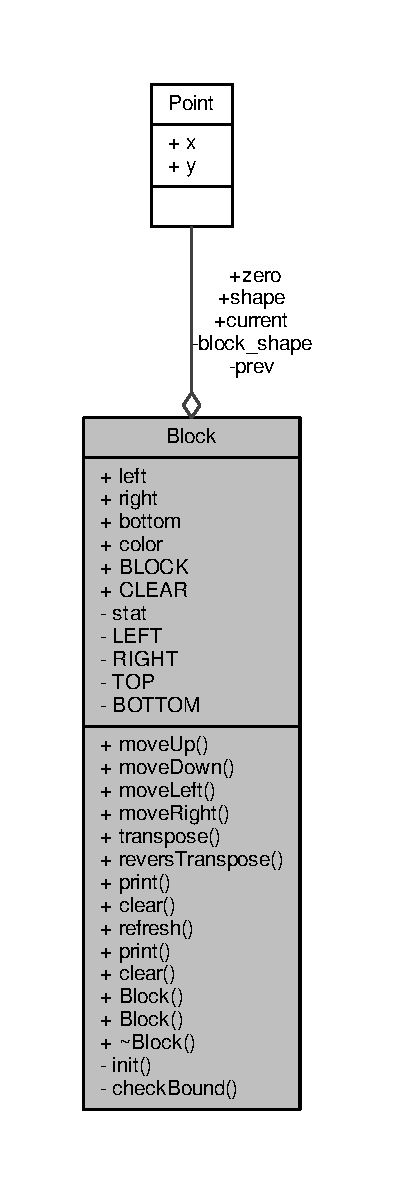
\includegraphics[height=550pt]{class_block__coll__graph}
\end{center}
\end{figure}
\subsection*{Public 멤버 함수}
\begin{DoxyCompactItemize}
\item 
void \hyperlink{class_block_a8bf4fce7b2b837fd49726b6a7f17f4b0}{move\+Up} ()
\item 
void \hyperlink{class_block_a947d677f5229eabb9ceb291e3552773d}{move\+Down} ()
\item 
void \hyperlink{class_block_af304df3662f2c6feec7cfc232246ef29}{move\+Left} ()
\item 
void \hyperlink{class_block_a13d1f87524fed8d686a4d478e41d5096}{move\+Right} ()
\item 
void \hyperlink{class_block_a9cc446ec51a125982c41e67af63059b0}{transpose} ()
\item 
void \hyperlink{class_block_a18bfe78145650d1b13267000feea278b}{revers\+Transpose} ()
\item 
void \hyperlink{class_block_a6735096bf1a9678a688b98782bd1b226}{print} (int x, int y)
\item 
void \hyperlink{class_block_a5ea55096829ff27961b989409283cd86}{clear} (int x, int y)
\item 
void \hyperlink{class_block_a24e9792df444cc3cd9cd9c28a62f5abd}{refresh} ()
\item 
void \hyperlink{class_block_a7ea913786e48c140a2a35ff03c35746c}{print} ()
\item 
void \hyperlink{class_block_ab2f8596ed64d7d4fc1ce6cbd739173de}{clear} ()
\item 
\hyperlink{class_block_a37658a946bf5067ad01d68d9ff086adc}{Block} ()
\item 
\hyperlink{class_block_a991643bd8dd22fc349c55b0aa7dcded3}{Block} (int type)
\item 
virtual \hyperlink{class_block_a19d1bd0e1cef6a865ed2745a2e648405}{$\sim$\+Block} ()
\end{DoxyCompactItemize}
\subsection*{Public 속성}
\begin{DoxyCompactItemize}
\item 
\hyperlink{struct_point}{Point} \hyperlink{class_block_aeb5dd312b719966752ba4b38720a4535}{current}
\item 
int \hyperlink{class_block_a1e4846853623ef67785a1bae5cec623e}{left}
\item 
int \hyperlink{class_block_a370e4fb56e296b92eb2cc3916b3f39b2}{right}
\item 
int \hyperlink{class_block_a8d97d8b0b6a09592ac007c13c3fa3867}{bottom}
\item 
int \hyperlink{class_block_a11fa34418f20b6613d0ceeea8fc71d25}{color}
\item 
\hyperlink{struct_point}{Point} \hyperlink{class_block_ae1a4e97236e1e5f04d21fc9227b8c3a8}{shape} \mbox{[}4\mbox{]}
\end{DoxyCompactItemize}
\subsection*{정적 Public 속성}
\begin{DoxyCompactItemize}
\item 
static const char $\ast$ \hyperlink{class_block_a4cb64c2c20884eed68c24c6147f68514}{B\+L\+O\+CK} = \char`\"{}\mbox{[}$\,$\mbox{]}\char`\"{}
\item 
static const char $\ast$ \hyperlink{class_block_a11bcda9589b54be35a8905ca7be7310e}{C\+L\+E\+AR} = \char`\"{} \char`\"{}
\item 
static \hyperlink{struct_point}{Point} \hyperlink{class_block_ad456f4794a480711f7057e1f270d93c2}{zero} = \hyperlink{struct_point}{Point}()
\end{DoxyCompactItemize}
\subsection*{Private 멤버 함수}
\begin{DoxyCompactItemize}
\item 
void \hyperlink{class_block_a35d1fdd5ff24816037fff5b419aaabb8}{init} (int type)
\item 
void \hyperlink{class_block_a4ce6f20dfa2c216f77cbc1a7f2a6f3a2}{check\+Bound} ()
\end{DoxyCompactItemize}
\subsection*{Private 속성}
\begin{DoxyCompactItemize}
\item 
int \hyperlink{class_block_a786c39534d84f71238f0189d8852e432}{stat}
\item 
\hyperlink{struct_point}{Point} \hyperlink{class_block_ab86ce4753987a3eb39058553fd81b462}{prev}
\end{DoxyCompactItemize}
\subsection*{정적 Private 속성}
\begin{DoxyCompactItemize}
\item 
static const int \hyperlink{class_block_ac5f5e2234205915a274e7aa43a476a62}{L\+E\+FT} =0
\item 
static const int \hyperlink{class_block_a446deab28dcc4d905bb33219eb6da3dc}{R\+I\+G\+HT} =\hyperlink{_game_logic_8h_a9649ab8139c4c2ea5c93625b30d92a05}{W\+I\+D\+TH}-\/1
\item 
static const int \hyperlink{class_block_a8609875a08b9ec9e07aec1e9ed1e6c7f}{T\+OP} =0
\item 
static const int \hyperlink{class_block_acae0f4fec218b09fc2ea00e6fa97f9a5}{B\+O\+T\+T\+OM} =\hyperlink{_game_logic_8h_af728b7647e0b8c49832983a31f9a2e9b}{H\+E\+I\+G\+HT}+1
\item 
static const \hyperlink{struct_point}{Point} \hyperlink{class_block_a87730d80e01cf50689abc8525d27f06d}{block\+\_\+shape} \mbox{[}$\,$\mbox{]}\mbox{[}4\mbox{]}\mbox{[}4\mbox{]}
\begin{DoxyCompactList}\small\item\em block embody \end{DoxyCompactList}\end{DoxyCompactItemize}


\subsection{상세한 설명}


Block.\+h 파일의 14 번째 라인에서 정의되었습니다.



\subsection{생성자 \& 소멸자 문서화}
\index{Block@{Block}!Block@{Block}}
\index{Block@{Block}!Block@{Block}}
\subsubsection[{\texorpdfstring{Block()}{Block()}}]{\setlength{\rightskip}{0pt plus 5cm}Block\+::\+Block (
\begin{DoxyParamCaption}
{}
\end{DoxyParamCaption}
)}\hypertarget{class_block_a37658a946bf5067ad01d68d9ff086adc}{}\label{class_block_a37658a946bf5067ad01d68d9ff086adc}


Block.\+cpp 파일의 105 번째 라인에서 정의되었습니다.


\begin{DoxyCode}
105              \{
106     \hyperlink{class_block_a35d1fdd5ff24816037fff5b419aaabb8}{init}(rand() % 7);
107 \}
\end{DoxyCode}


이 함수 내부에서 호출하는 함수들에 대한 그래프입니다.\+:
\nopagebreak
\begin{figure}[H]
\begin{center}
\leavevmode
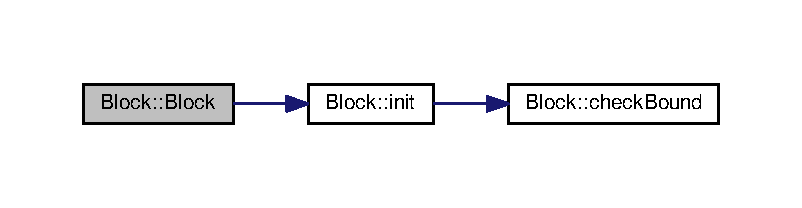
\includegraphics[width=350pt]{class_block_a37658a946bf5067ad01d68d9ff086adc_cgraph}
\end{center}
\end{figure}


\index{Block@{Block}!Block@{Block}}
\index{Block@{Block}!Block@{Block}}
\subsubsection[{\texorpdfstring{Block(int type)}{Block(int type)}}]{\setlength{\rightskip}{0pt plus 5cm}Block\+::\+Block (
\begin{DoxyParamCaption}
\item[{int}]{type}
\end{DoxyParamCaption}
)}\hypertarget{class_block_a991643bd8dd22fc349c55b0aa7dcded3}{}\label{class_block_a991643bd8dd22fc349c55b0aa7dcded3}


Block.\+cpp 파일의 111 번째 라인에서 정의되었습니다.


\begin{DoxyCode}
111                      \{
112     \hyperlink{class_block_a35d1fdd5ff24816037fff5b419aaabb8}{init}(type);
113 \}
\end{DoxyCode}


이 함수 내부에서 호출하는 함수들에 대한 그래프입니다.\+:
\nopagebreak
\begin{figure}[H]
\begin{center}
\leavevmode
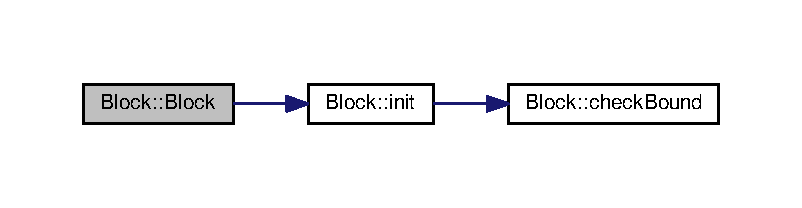
\includegraphics[width=350pt]{class_block_a991643bd8dd22fc349c55b0aa7dcded3_cgraph}
\end{center}
\end{figure}


\index{Block@{Block}!````~Block@{$\sim$\+Block}}
\index{````~Block@{$\sim$\+Block}!Block@{Block}}
\subsubsection[{\texorpdfstring{$\sim$\+Block()}{~Block()}}]{\setlength{\rightskip}{0pt plus 5cm}Block\+::$\sim$\+Block (
\begin{DoxyParamCaption}
{}
\end{DoxyParamCaption}
)\hspace{0.3cm}{\ttfamily [virtual]}}\hypertarget{class_block_a19d1bd0e1cef6a865ed2745a2e648405}{}\label{class_block_a19d1bd0e1cef6a865ed2745a2e648405}
\begin{DoxyRefDesc}{할일}
\item[\hyperlink{todo__todo000001}{할일}]Auto-\/generated destructor stub\end{DoxyRefDesc}


Block.\+cpp 파일의 115 번째 라인에서 정의되었습니다.


\begin{DoxyCode}
115               \{
121 \}
\end{DoxyCode}


\subsection{멤버 함수 문서화}
\index{Block@{Block}!check\+Bound@{check\+Bound}}
\index{check\+Bound@{check\+Bound}!Block@{Block}}
\subsubsection[{\texorpdfstring{check\+Bound()}{checkBound()}}]{\setlength{\rightskip}{0pt plus 5cm}void Block\+::check\+Bound (
\begin{DoxyParamCaption}
{}
\end{DoxyParamCaption}
)\hspace{0.3cm}{\ttfamily [private]}}\hypertarget{class_block_a4ce6f20dfa2c216f77cbc1a7f2a6f3a2}{}\label{class_block_a4ce6f20dfa2c216f77cbc1a7f2a6f3a2}


Block.\+cpp 파일의 208 번째 라인에서 정의되었습니다.


\begin{DoxyCode}
208                        \{
209     \textcolor{keywordtype}{int} maxX = -10, minX = 10, maxY = -10;
210 
211     \textcolor{keywordflow}{for} (\textcolor{keywordtype}{int} i = 0; i < 4; i++) \{
212         \textcolor{keywordflow}{if} (\hyperlink{class_block_ae1a4e97236e1e5f04d21fc9227b8c3a8}{shape}[i].x > maxX) \{
213             maxX = \hyperlink{class_block_ae1a4e97236e1e5f04d21fc9227b8c3a8}{shape}[i].\hyperlink{struct_point_a8c779e11e694b20e0946105a9f5de842}{x};
214         \}
215         \textcolor{keywordflow}{if} (\hyperlink{class_block_ae1a4e97236e1e5f04d21fc9227b8c3a8}{shape}[i].x < minX) \{
216             minX = \hyperlink{class_block_ae1a4e97236e1e5f04d21fc9227b8c3a8}{shape}[i].\hyperlink{struct_point_a8c779e11e694b20e0946105a9f5de842}{x};
217         \}
218         \textcolor{keywordflow}{if} (\hyperlink{class_block_ae1a4e97236e1e5f04d21fc9227b8c3a8}{shape}[i].y > maxY) \{
219             maxY = \hyperlink{class_block_ae1a4e97236e1e5f04d21fc9227b8c3a8}{shape}[i].\hyperlink{struct_point_a2e1b5fb2b2a83571f5c0bc0f66a73cf7}{y};
220         \}
221     \}
222     \hyperlink{class_block_a1e4846853623ef67785a1bae5cec623e}{left} = minX;
223     \hyperlink{class_block_a370e4fb56e296b92eb2cc3916b3f39b2}{right} = maxX;
224     \hyperlink{class_block_a8d97d8b0b6a09592ac007c13c3fa3867}{bottom} = maxY;
225 \}
\end{DoxyCode}


이 함수를 호출하는 함수들에 대한 그래프입니다.\+:
\nopagebreak
\begin{figure}[H]
\begin{center}
\leavevmode
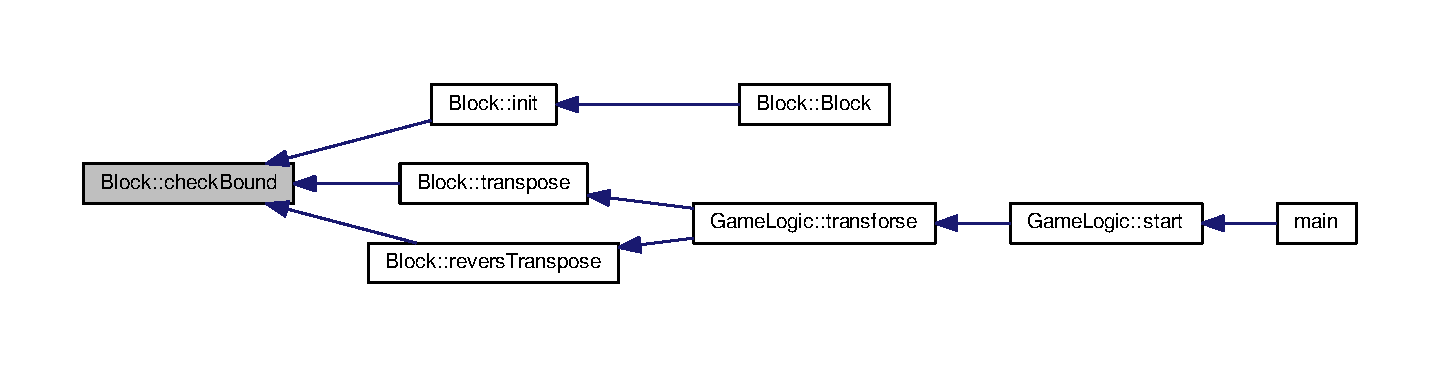
\includegraphics[width=350pt]{class_block_a4ce6f20dfa2c216f77cbc1a7f2a6f3a2_icgraph}
\end{center}
\end{figure}


\index{Block@{Block}!clear@{clear}}
\index{clear@{clear}!Block@{Block}}
\subsubsection[{\texorpdfstring{clear(int x, int y)}{clear(int x, int y)}}]{\setlength{\rightskip}{0pt plus 5cm}void Block\+::clear (
\begin{DoxyParamCaption}
\item[{int}]{x, }
\item[{int}]{y}
\end{DoxyParamCaption}
)}\hypertarget{class_block_a5ea55096829ff27961b989409283cd86}{}\label{class_block_a5ea55096829ff27961b989409283cd86}


Block.\+cpp 파일의 202 번째 라인에서 정의되었습니다.


\begin{DoxyCode}
202                               \{
203     \textcolor{keywordflow}{for} (\textcolor{keywordtype}{int} i = 0; i < 4; i++) \{
204         \hyperlink{myio_8cpp_afce36429cc875312f4476969820ebb51}{printColorString}(\hyperlink{class_block_ae1a4e97236e1e5f04d21fc9227b8c3a8}{shape}[i].x * 2 + x , \hyperlink{class_block_ae1a4e97236e1e5f04d21fc9227b8c3a8}{shape}[i].y  + y , 
      \hyperlink{myio_8h_a56e1aea61ee305e3648158362333b3a8}{COLOR\_DEFAULT}, \hyperlink{class_block_a11bcda9589b54be35a8905ca7be7310e}{CLEAR});
205     \}
206 \}
\end{DoxyCode}


이 함수 내부에서 호출하는 함수들에 대한 그래프입니다.\+:
\nopagebreak
\begin{figure}[H]
\begin{center}
\leavevmode
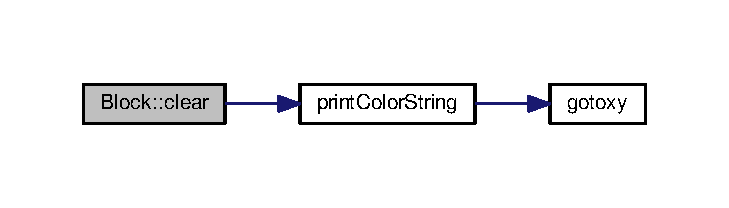
\includegraphics[width=350pt]{class_block_a5ea55096829ff27961b989409283cd86_cgraph}
\end{center}
\end{figure}




이 함수를 호출하는 함수들에 대한 그래프입니다.\+:
\nopagebreak
\begin{figure}[H]
\begin{center}
\leavevmode
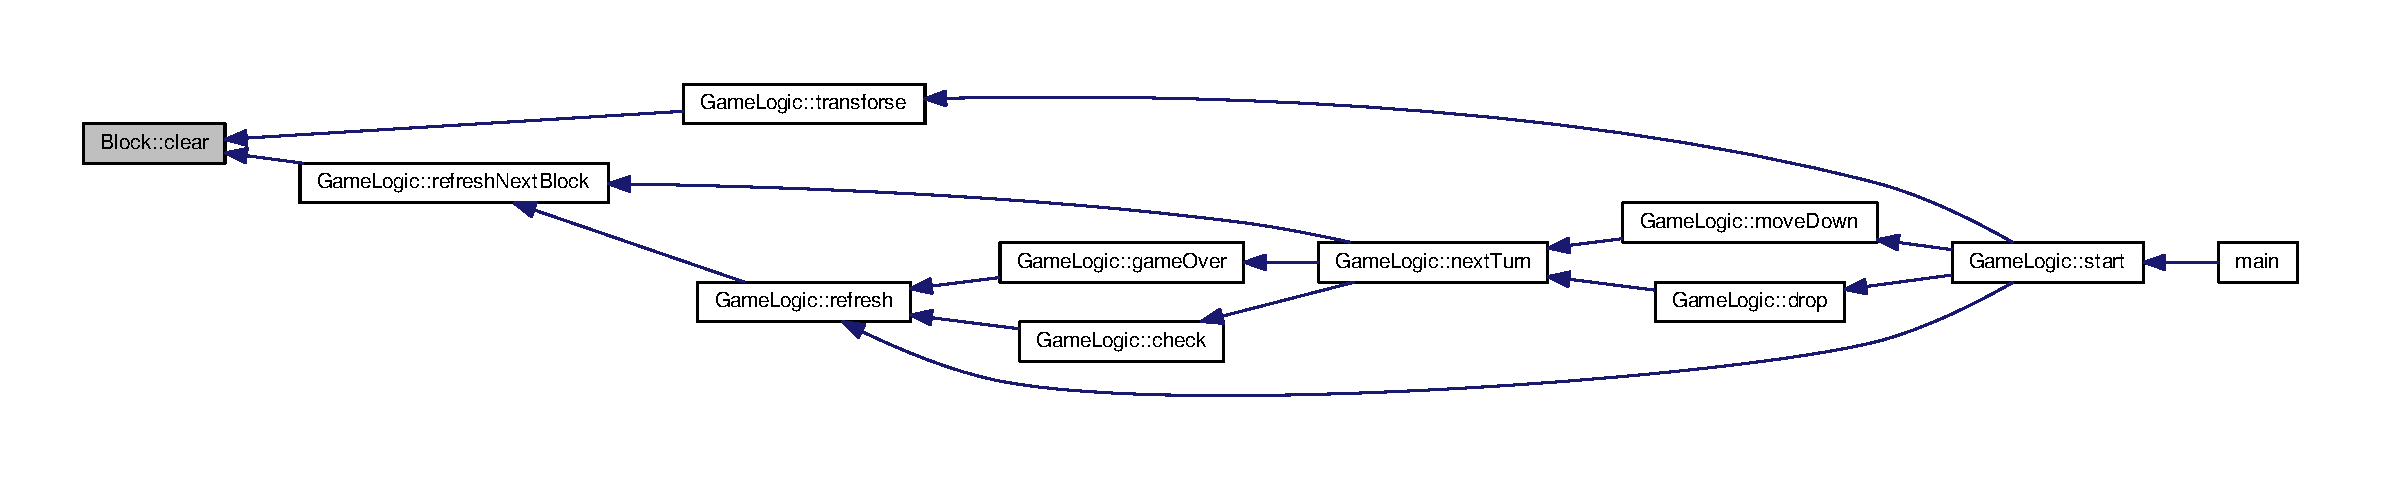
\includegraphics[width=350pt]{class_block_a5ea55096829ff27961b989409283cd86_icgraph}
\end{center}
\end{figure}


\index{Block@{Block}!clear@{clear}}
\index{clear@{clear}!Block@{Block}}
\subsubsection[{\texorpdfstring{clear()}{clear()}}]{\setlength{\rightskip}{0pt plus 5cm}void Block\+::clear (
\begin{DoxyParamCaption}
{}
\end{DoxyParamCaption}
)}\hypertarget{class_block_ab2f8596ed64d7d4fc1ce6cbd739173de}{}\label{class_block_ab2f8596ed64d7d4fc1ce6cbd739173de}


Block.\+cpp 파일의 183 번째 라인에서 정의되었습니다.


\begin{DoxyCode}
183                   \{
184     \textcolor{keywordflow}{for} (\textcolor{keywordtype}{int} i = 0; i < 4; i++) \{
185         \hyperlink{myio_8cpp_afce36429cc875312f4476969820ebb51}{printColorString}(\hyperlink{class_block_ae1a4e97236e1e5f04d21fc9227b8c3a8}{shape}[i].x * 2 + \hyperlink{class_block_ab86ce4753987a3eb39058553fd81b462}{prev}.\hyperlink{struct_point_a8c779e11e694b20e0946105a9f5de842}{x} * 2 + 
      \hyperlink{class_block_ad456f4794a480711f7057e1f270d93c2}{zero}.\hyperlink{struct_point_a8c779e11e694b20e0946105a9f5de842}{x}, \hyperlink{class_block_ae1a4e97236e1e5f04d21fc9227b8c3a8}{shape}[i].\hyperlink{struct_point_a2e1b5fb2b2a83571f5c0bc0f66a73cf7}{y} + \hyperlink{class_block_ab86ce4753987a3eb39058553fd81b462}{prev}.\hyperlink{struct_point_a2e1b5fb2b2a83571f5c0bc0f66a73cf7}{y} + \hyperlink{class_block_ad456f4794a480711f7057e1f270d93c2}{zero}.\hyperlink{struct_point_a2e1b5fb2b2a83571f5c0bc0f66a73cf7}{y}, \hyperlink{myio_8h_a56e1aea61ee305e3648158362333b3a8}{COLOR\_DEFAULT}, 
      \hyperlink{class_block_a11bcda9589b54be35a8905ca7be7310e}{CLEAR});
186     \}
187 \}
\end{DoxyCode}


이 함수 내부에서 호출하는 함수들에 대한 그래프입니다.\+:
\nopagebreak
\begin{figure}[H]
\begin{center}
\leavevmode
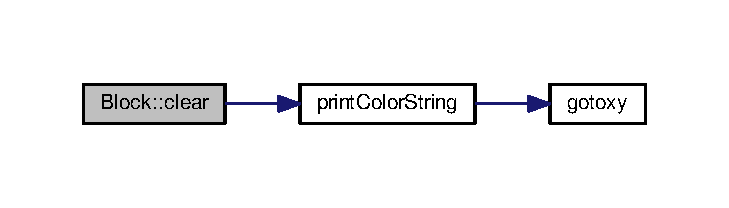
\includegraphics[width=350pt]{class_block_ab2f8596ed64d7d4fc1ce6cbd739173de_cgraph}
\end{center}
\end{figure}




이 함수를 호출하는 함수들에 대한 그래프입니다.\+:
\nopagebreak
\begin{figure}[H]
\begin{center}
\leavevmode
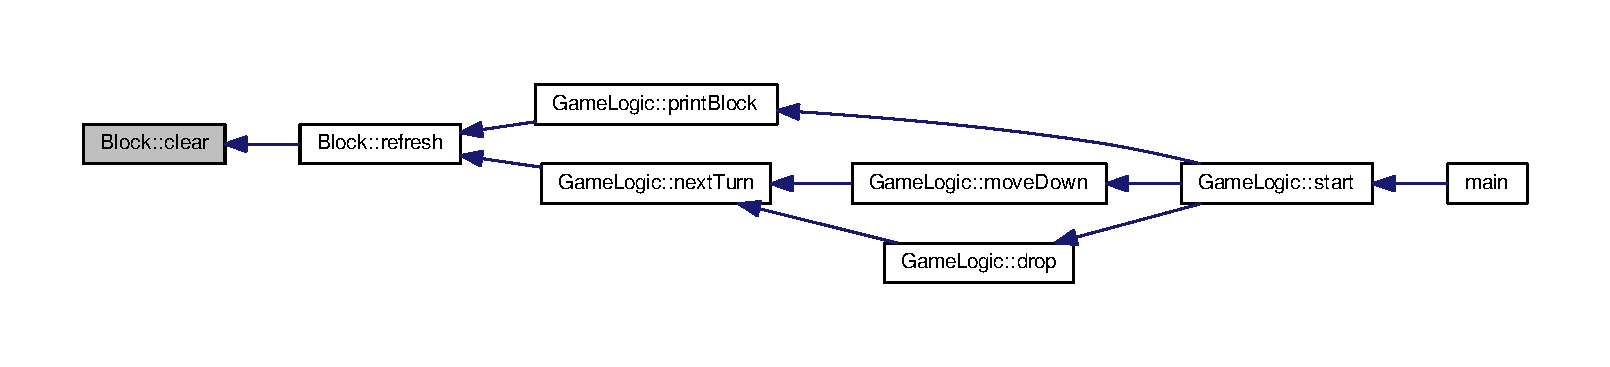
\includegraphics[width=350pt]{class_block_ab2f8596ed64d7d4fc1ce6cbd739173de_icgraph}
\end{center}
\end{figure}


\index{Block@{Block}!init@{init}}
\index{init@{init}!Block@{Block}}
\subsubsection[{\texorpdfstring{init(int type)}{init(int type)}}]{\setlength{\rightskip}{0pt plus 5cm}void Block\+::init (
\begin{DoxyParamCaption}
\item[{int}]{type}
\end{DoxyParamCaption}
)\hspace{0.3cm}{\ttfamily [private]}}\hypertarget{class_block_a35d1fdd5ff24816037fff5b419aaabb8}{}\label{class_block_a35d1fdd5ff24816037fff5b419aaabb8}


Block.\+cpp 파일의 122 번째 라인에서 정의되었습니다.


\begin{DoxyCode}
122                          \{
123     \hyperlink{class_block_a786c39534d84f71238f0189d8852e432}{stat} = 0;
124     \hyperlink{class_block_a11fa34418f20b6613d0ceeea8fc71d25}{color} = type % 7;
125     \hyperlink{class_block_ae1a4e97236e1e5f04d21fc9227b8c3a8}{shape}[0] = \hyperlink{class_block_a87730d80e01cf50689abc8525d27f06d}{Block::block\_shape}[\hyperlink{class_block_a11fa34418f20b6613d0ceeea8fc71d25}{color}][\hyperlink{class_block_a786c39534d84f71238f0189d8852e432}{stat}][0];
126     \hyperlink{class_block_ae1a4e97236e1e5f04d21fc9227b8c3a8}{shape}[1] = \hyperlink{class_block_a87730d80e01cf50689abc8525d27f06d}{Block::block\_shape}[\hyperlink{class_block_a11fa34418f20b6613d0ceeea8fc71d25}{color}][\hyperlink{class_block_a786c39534d84f71238f0189d8852e432}{stat}][1];
127     \hyperlink{class_block_ae1a4e97236e1e5f04d21fc9227b8c3a8}{shape}[2] = \hyperlink{class_block_a87730d80e01cf50689abc8525d27f06d}{Block::block\_shape}[\hyperlink{class_block_a11fa34418f20b6613d0ceeea8fc71d25}{color}][\hyperlink{class_block_a786c39534d84f71238f0189d8852e432}{stat}][2];
128     \hyperlink{class_block_ae1a4e97236e1e5f04d21fc9227b8c3a8}{shape}[3] = \hyperlink{class_block_a87730d80e01cf50689abc8525d27f06d}{Block::block\_shape}[\hyperlink{class_block_a11fa34418f20b6613d0ceeea8fc71d25}{color}][\hyperlink{class_block_a786c39534d84f71238f0189d8852e432}{stat}][3];
129     \hyperlink{class_block_a11fa34418f20b6613d0ceeea8fc71d25}{color} += 41;
130     \hyperlink{class_block_aeb5dd312b719966752ba4b38720a4535}{current}.\hyperlink{struct_point_a8c779e11e694b20e0946105a9f5de842}{x} = \hyperlink{class_block_ac5f5e2234205915a274e7aa43a476a62}{LEFT} + 3;
131     \hyperlink{class_block_aeb5dd312b719966752ba4b38720a4535}{current}.\hyperlink{struct_point_a2e1b5fb2b2a83571f5c0bc0f66a73cf7}{y} = \hyperlink{class_block_a8609875a08b9ec9e07aec1e9ed1e6c7f}{TOP};
132     \hyperlink{class_block_ab86ce4753987a3eb39058553fd81b462}{prev} = \hyperlink{class_block_aeb5dd312b719966752ba4b38720a4535}{current};
133     \hyperlink{class_block_a4ce6f20dfa2c216f77cbc1a7f2a6f3a2}{checkBound}();
134 \}
\end{DoxyCode}


이 함수 내부에서 호출하는 함수들에 대한 그래프입니다.\+:
\nopagebreak
\begin{figure}[H]
\begin{center}
\leavevmode
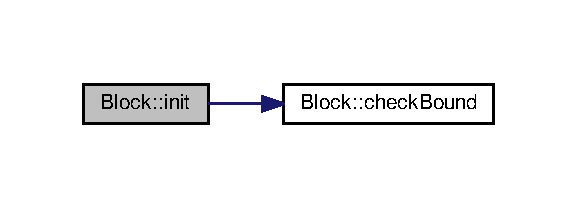
\includegraphics[width=277pt]{class_block_a35d1fdd5ff24816037fff5b419aaabb8_cgraph}
\end{center}
\end{figure}




이 함수를 호출하는 함수들에 대한 그래프입니다.\+:
\nopagebreak
\begin{figure}[H]
\begin{center}
\leavevmode
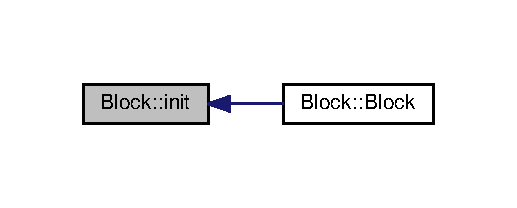
\includegraphics[width=248pt]{class_block_a35d1fdd5ff24816037fff5b419aaabb8_icgraph}
\end{center}
\end{figure}


\index{Block@{Block}!move\+Down@{move\+Down}}
\index{move\+Down@{move\+Down}!Block@{Block}}
\subsubsection[{\texorpdfstring{move\+Down()}{moveDown()}}]{\setlength{\rightskip}{0pt plus 5cm}void Block\+::move\+Down (
\begin{DoxyParamCaption}
{}
\end{DoxyParamCaption}
)}\hypertarget{class_block_a947d677f5229eabb9ceb291e3552773d}{}\label{class_block_a947d677f5229eabb9ceb291e3552773d}


Block.\+cpp 파일의 162 번째 라인에서 정의되었습니다.


\begin{DoxyCode}
162                      \{
163 
164     \textcolor{keywordflow}{if} (\hyperlink{class_block_aeb5dd312b719966752ba4b38720a4535}{current}.\hyperlink{struct_point_a2e1b5fb2b2a83571f5c0bc0f66a73cf7}{y} + \hyperlink{class_block_a8d97d8b0b6a09592ac007c13c3fa3867}{bottom} < \hyperlink{class_block_acae0f4fec218b09fc2ea00e6fa97f9a5}{BOTTOM})
165         \hyperlink{class_block_aeb5dd312b719966752ba4b38720a4535}{current}.\hyperlink{struct_point_a2e1b5fb2b2a83571f5c0bc0f66a73cf7}{y}++;
166 
167 \}
\end{DoxyCode}


이 함수를 호출하는 함수들에 대한 그래프입니다.\+:
\nopagebreak
\begin{figure}[H]
\begin{center}
\leavevmode
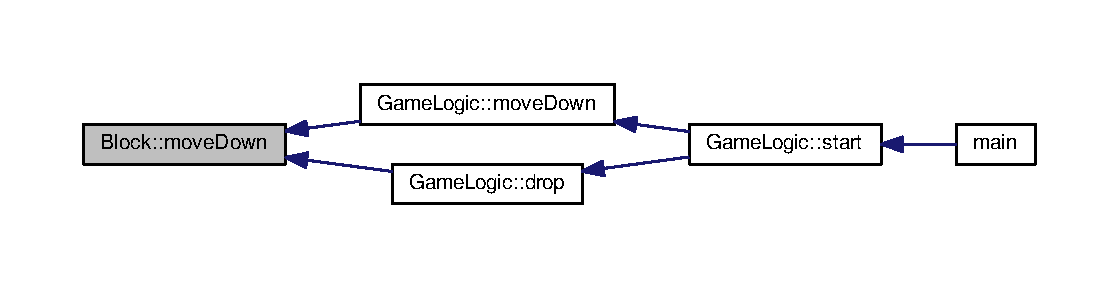
\includegraphics[width=350pt]{class_block_a947d677f5229eabb9ceb291e3552773d_icgraph}
\end{center}
\end{figure}


\index{Block@{Block}!move\+Left@{move\+Left}}
\index{move\+Left@{move\+Left}!Block@{Block}}
\subsubsection[{\texorpdfstring{move\+Left()}{moveLeft()}}]{\setlength{\rightskip}{0pt plus 5cm}void Block\+::move\+Left (
\begin{DoxyParamCaption}
{}
\end{DoxyParamCaption}
)}\hypertarget{class_block_af304df3662f2c6feec7cfc232246ef29}{}\label{class_block_af304df3662f2c6feec7cfc232246ef29}


Block.\+cpp 파일의 172 번째 라인에서 정의되었습니다.


\begin{DoxyCode}
172                      \{
173     \textcolor{keywordflow}{if} (\hyperlink{class_block_aeb5dd312b719966752ba4b38720a4535}{current}.\hyperlink{struct_point_a8c779e11e694b20e0946105a9f5de842}{x} + \hyperlink{class_block_a1e4846853623ef67785a1bae5cec623e}{left} > \hyperlink{class_block_ac5f5e2234205915a274e7aa43a476a62}{LEFT})
174         \hyperlink{class_block_aeb5dd312b719966752ba4b38720a4535}{current}.\hyperlink{struct_point_a8c779e11e694b20e0946105a9f5de842}{x}--;
175 
176 \}
\end{DoxyCode}


이 함수를 호출하는 함수들에 대한 그래프입니다.\+:
\nopagebreak
\begin{figure}[H]
\begin{center}
\leavevmode
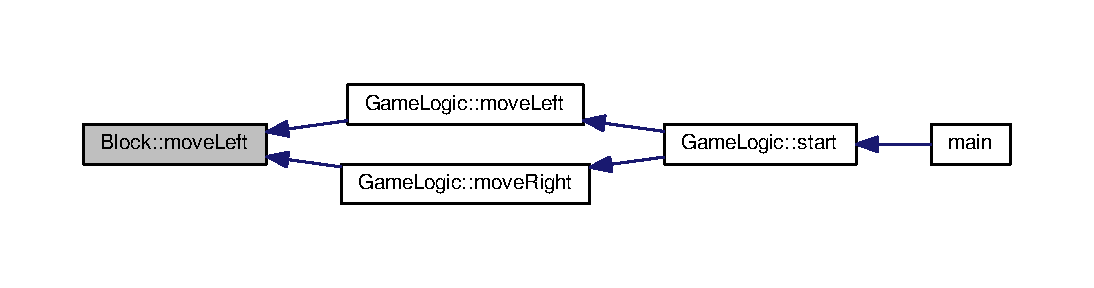
\includegraphics[width=350pt]{class_block_af304df3662f2c6feec7cfc232246ef29_icgraph}
\end{center}
\end{figure}


\index{Block@{Block}!move\+Right@{move\+Right}}
\index{move\+Right@{move\+Right}!Block@{Block}}
\subsubsection[{\texorpdfstring{move\+Right()}{moveRight()}}]{\setlength{\rightskip}{0pt plus 5cm}void Block\+::move\+Right (
\begin{DoxyParamCaption}
{}
\end{DoxyParamCaption}
)}\hypertarget{class_block_a13d1f87524fed8d686a4d478e41d5096}{}\label{class_block_a13d1f87524fed8d686a4d478e41d5096}


Block.\+cpp 파일의 168 번째 라인에서 정의되었습니다.


\begin{DoxyCode}
168                       \{
169     \textcolor{keywordflow}{if} (\hyperlink{class_block_aeb5dd312b719966752ba4b38720a4535}{current}.\hyperlink{struct_point_a8c779e11e694b20e0946105a9f5de842}{x} + \hyperlink{class_block_a370e4fb56e296b92eb2cc3916b3f39b2}{right} < \hyperlink{class_block_a446deab28dcc4d905bb33219eb6da3dc}{RIGHT})
170         \hyperlink{class_block_aeb5dd312b719966752ba4b38720a4535}{current}.\hyperlink{struct_point_a8c779e11e694b20e0946105a9f5de842}{x}++;
171 \}
\end{DoxyCode}


이 함수를 호출하는 함수들에 대한 그래프입니다.\+:
\nopagebreak
\begin{figure}[H]
\begin{center}
\leavevmode
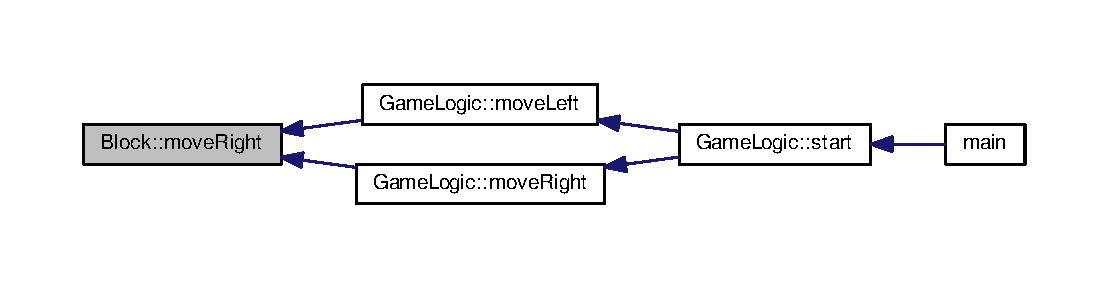
\includegraphics[width=350pt]{class_block_a13d1f87524fed8d686a4d478e41d5096_icgraph}
\end{center}
\end{figure}


\index{Block@{Block}!move\+Up@{move\+Up}}
\index{move\+Up@{move\+Up}!Block@{Block}}
\subsubsection[{\texorpdfstring{move\+Up()}{moveUp()}}]{\setlength{\rightskip}{0pt plus 5cm}void Block\+::move\+Up (
\begin{DoxyParamCaption}
{}
\end{DoxyParamCaption}
)}\hypertarget{class_block_a8bf4fce7b2b837fd49726b6a7f17f4b0}{}\label{class_block_a8bf4fce7b2b837fd49726b6a7f17f4b0}


Block.\+cpp 파일의 156 번째 라인에서 정의되었습니다.


\begin{DoxyCode}
156                    \{
157 
158     \textcolor{keywordflow}{if} (\hyperlink{class_block_aeb5dd312b719966752ba4b38720a4535}{current}.\hyperlink{struct_point_a2e1b5fb2b2a83571f5c0bc0f66a73cf7}{y} > \hyperlink{class_block_a8609875a08b9ec9e07aec1e9ed1e6c7f}{TOP})
159         \hyperlink{class_block_aeb5dd312b719966752ba4b38720a4535}{current}.\hyperlink{struct_point_a2e1b5fb2b2a83571f5c0bc0f66a73cf7}{y}--;
160 \}
\end{DoxyCode}


이 함수를 호출하는 함수들에 대한 그래프입니다.\+:
\nopagebreak
\begin{figure}[H]
\begin{center}
\leavevmode
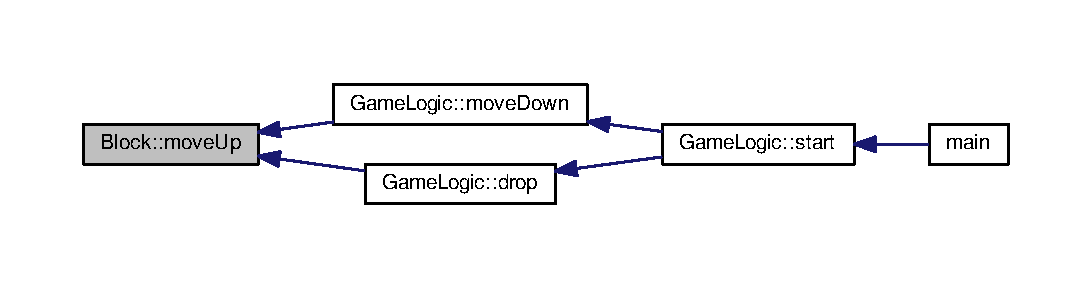
\includegraphics[width=350pt]{class_block_a8bf4fce7b2b837fd49726b6a7f17f4b0_icgraph}
\end{center}
\end{figure}


\index{Block@{Block}!print@{print}}
\index{print@{print}!Block@{Block}}
\subsubsection[{\texorpdfstring{print(int x, int y)}{print(int x, int y)}}]{\setlength{\rightskip}{0pt plus 5cm}void Block\+::print (
\begin{DoxyParamCaption}
\item[{int}]{x, }
\item[{int}]{y}
\end{DoxyParamCaption}
)}\hypertarget{class_block_a6735096bf1a9678a688b98782bd1b226}{}\label{class_block_a6735096bf1a9678a688b98782bd1b226}


Block.\+cpp 파일의 196 번째 라인에서 정의되었습니다.


\begin{DoxyCode}
196                               \{
197     \textcolor{keywordflow}{for} (\textcolor{keywordtype}{int} i = 0; i < 4; i++) \{
198         \hyperlink{myio_8cpp_afce36429cc875312f4476969820ebb51}{printColorString}(\hyperlink{class_block_ae1a4e97236e1e5f04d21fc9227b8c3a8}{shape}[i].x * 2  + x , \hyperlink{class_block_ae1a4e97236e1e5f04d21fc9227b8c3a8}{shape}[i].y  + y , 
      \hyperlink{class_block_a11fa34418f20b6613d0ceeea8fc71d25}{color}, \hyperlink{class_block_a4cb64c2c20884eed68c24c6147f68514}{BLOCK});
199     \}
200 \}
\end{DoxyCode}


이 함수 내부에서 호출하는 함수들에 대한 그래프입니다.\+:
\nopagebreak
\begin{figure}[H]
\begin{center}
\leavevmode
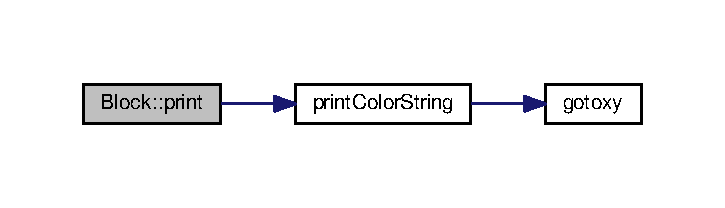
\includegraphics[width=348pt]{class_block_a6735096bf1a9678a688b98782bd1b226_cgraph}
\end{center}
\end{figure}




이 함수를 호출하는 함수들에 대한 그래프입니다.\+:
\nopagebreak
\begin{figure}[H]
\begin{center}
\leavevmode
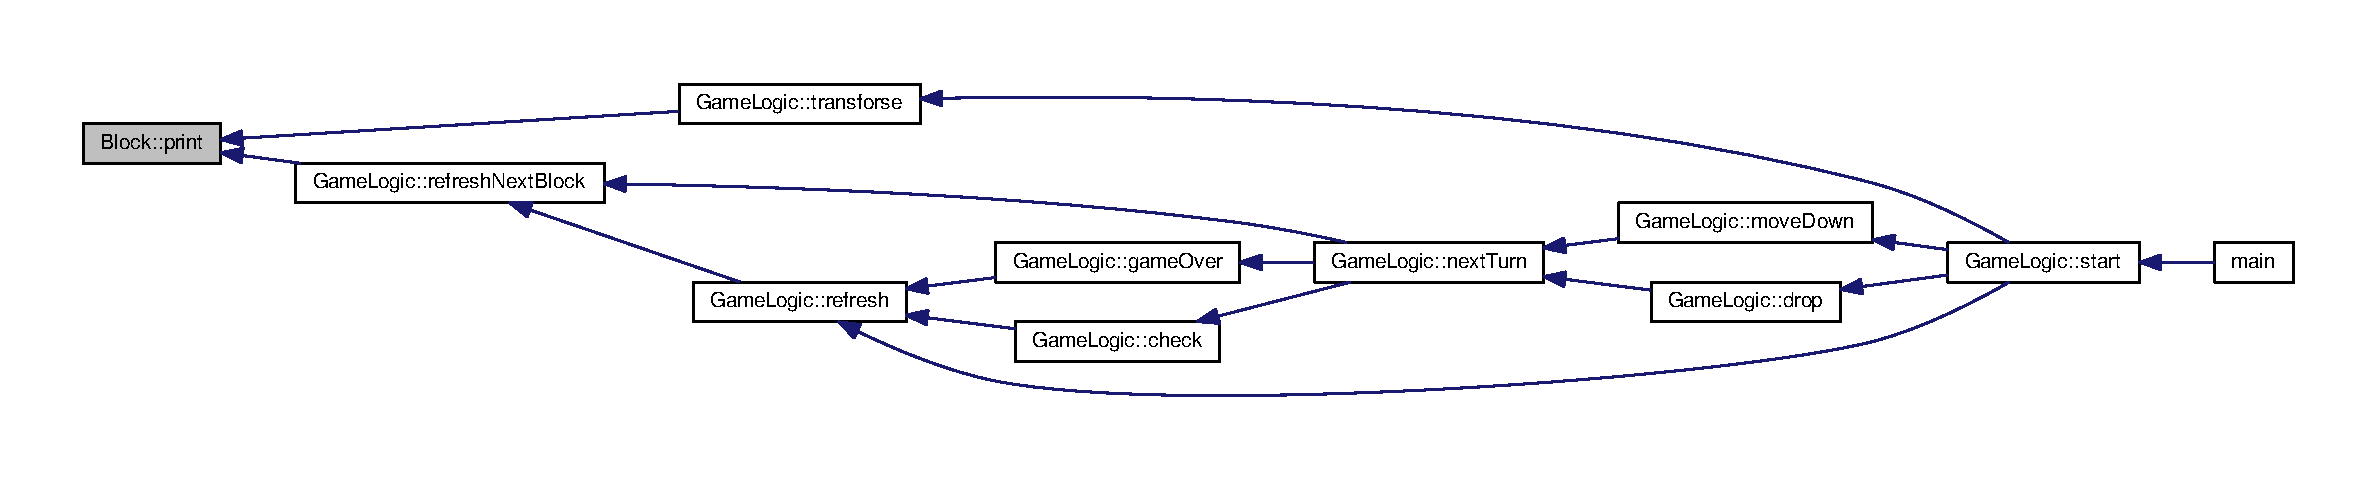
\includegraphics[width=350pt]{class_block_a6735096bf1a9678a688b98782bd1b226_icgraph}
\end{center}
\end{figure}


\index{Block@{Block}!print@{print}}
\index{print@{print}!Block@{Block}}
\subsubsection[{\texorpdfstring{print()}{print()}}]{\setlength{\rightskip}{0pt plus 5cm}void Block\+::print (
\begin{DoxyParamCaption}
{}
\end{DoxyParamCaption}
)}\hypertarget{class_block_a7ea913786e48c140a2a35ff03c35746c}{}\label{class_block_a7ea913786e48c140a2a35ff03c35746c}


Block.\+cpp 파일의 177 번째 라인에서 정의되었습니다.


\begin{DoxyCode}
177                   \{
178     \textcolor{keywordflow}{for} (\textcolor{keywordtype}{int} i = 0; i < 4; i++) \{
179         \hyperlink{myio_8cpp_afce36429cc875312f4476969820ebb51}{printColorString}(\hyperlink{class_block_ae1a4e97236e1e5f04d21fc9227b8c3a8}{shape}[i].x * 2 + \hyperlink{class_block_aeb5dd312b719966752ba4b38720a4535}{current}.\hyperlink{struct_point_a8c779e11e694b20e0946105a9f5de842}{x} * 2 + 
      \hyperlink{class_block_ad456f4794a480711f7057e1f270d93c2}{zero}.\hyperlink{struct_point_a8c779e11e694b20e0946105a9f5de842}{x}, \hyperlink{class_block_ae1a4e97236e1e5f04d21fc9227b8c3a8}{shape}[i].\hyperlink{struct_point_a2e1b5fb2b2a83571f5c0bc0f66a73cf7}{y} + \hyperlink{class_block_aeb5dd312b719966752ba4b38720a4535}{current}.\hyperlink{struct_point_a2e1b5fb2b2a83571f5c0bc0f66a73cf7}{y} + \hyperlink{class_block_ad456f4794a480711f7057e1f270d93c2}{zero}.\hyperlink{struct_point_a2e1b5fb2b2a83571f5c0bc0f66a73cf7}{y}, \hyperlink{class_block_a11fa34418f20b6613d0ceeea8fc71d25}{color}, 
      \hyperlink{class_block_a4cb64c2c20884eed68c24c6147f68514}{BLOCK});
180     \}
181     \hyperlink{class_block_ab86ce4753987a3eb39058553fd81b462}{prev} = \hyperlink{class_block_aeb5dd312b719966752ba4b38720a4535}{current};
182 \}
\end{DoxyCode}


이 함수 내부에서 호출하는 함수들에 대한 그래프입니다.\+:
\nopagebreak
\begin{figure}[H]
\begin{center}
\leavevmode
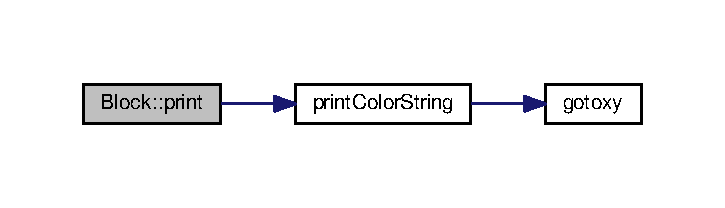
\includegraphics[width=348pt]{class_block_a7ea913786e48c140a2a35ff03c35746c_cgraph}
\end{center}
\end{figure}




이 함수를 호출하는 함수들에 대한 그래프입니다.\+:
\nopagebreak
\begin{figure}[H]
\begin{center}
\leavevmode
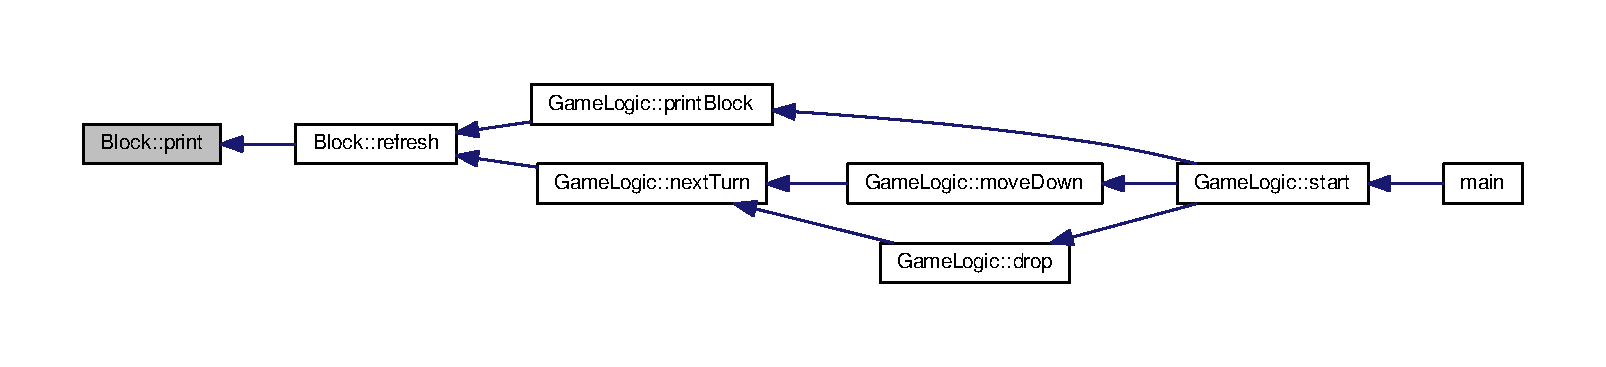
\includegraphics[width=350pt]{class_block_a7ea913786e48c140a2a35ff03c35746c_icgraph}
\end{center}
\end{figure}


\index{Block@{Block}!refresh@{refresh}}
\index{refresh@{refresh}!Block@{Block}}
\subsubsection[{\texorpdfstring{refresh()}{refresh()}}]{\setlength{\rightskip}{0pt plus 5cm}void Block\+::refresh (
\begin{DoxyParamCaption}
{}
\end{DoxyParamCaption}
)}\hypertarget{class_block_a24e9792df444cc3cd9cd9c28a62f5abd}{}\label{class_block_a24e9792df444cc3cd9cd9c28a62f5abd}


Block.\+cpp 파일의 189 번째 라인에서 정의되었습니다.


\begin{DoxyCode}
189                     \{
190 
191     \hyperlink{class_block_ab2f8596ed64d7d4fc1ce6cbd739173de}{clear}();
192     \hyperlink{class_block_a7ea913786e48c140a2a35ff03c35746c}{print}();
193     \hyperlink{class_block_ab86ce4753987a3eb39058553fd81b462}{prev} = \hyperlink{class_block_aeb5dd312b719966752ba4b38720a4535}{current};
194 \}
\end{DoxyCode}


이 함수 내부에서 호출하는 함수들에 대한 그래프입니다.\+:
\nopagebreak
\begin{figure}[H]
\begin{center}
\leavevmode
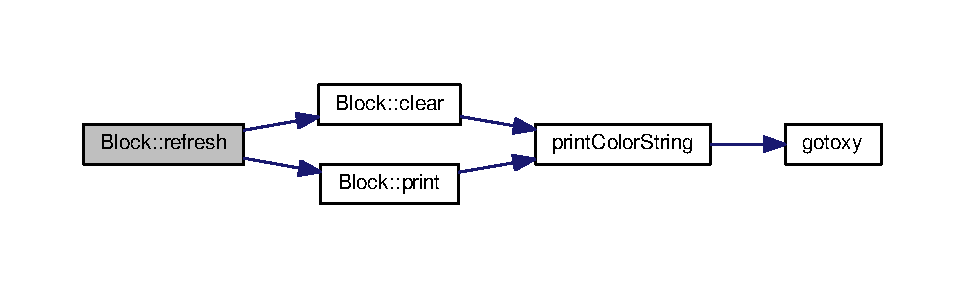
\includegraphics[width=350pt]{class_block_a24e9792df444cc3cd9cd9c28a62f5abd_cgraph}
\end{center}
\end{figure}




이 함수를 호출하는 함수들에 대한 그래프입니다.\+:
\nopagebreak
\begin{figure}[H]
\begin{center}
\leavevmode
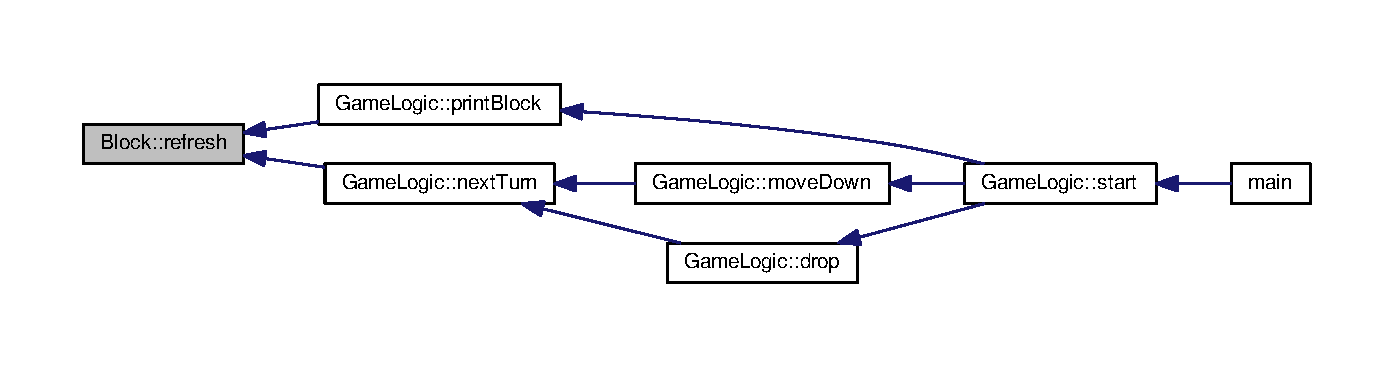
\includegraphics[width=350pt]{class_block_a24e9792df444cc3cd9cd9c28a62f5abd_icgraph}
\end{center}
\end{figure}


\index{Block@{Block}!revers\+Transpose@{revers\+Transpose}}
\index{revers\+Transpose@{revers\+Transpose}!Block@{Block}}
\subsubsection[{\texorpdfstring{revers\+Transpose()}{reversTranspose()}}]{\setlength{\rightskip}{0pt plus 5cm}void Block\+::revers\+Transpose (
\begin{DoxyParamCaption}
{}
\end{DoxyParamCaption}
)}\hypertarget{class_block_a18bfe78145650d1b13267000feea278b}{}\label{class_block_a18bfe78145650d1b13267000feea278b}


Block.\+cpp 파일의 145 번째 라인에서 정의되었습니다.


\begin{DoxyCode}
145                             \{
146 
147     \textcolor{keywordtype}{int} s = \hyperlink{class_block_a11fa34418f20b6613d0ceeea8fc71d25}{color} - 41;
148     \hyperlink{class_block_a786c39534d84f71238f0189d8852e432}{stat} = (\hyperlink{class_block_a786c39534d84f71238f0189d8852e432}{stat} + 3) % 4;
149     \hyperlink{class_block_ae1a4e97236e1e5f04d21fc9227b8c3a8}{shape}[0] = \hyperlink{class_block_a87730d80e01cf50689abc8525d27f06d}{Block::block\_shape}[s][\hyperlink{class_block_a786c39534d84f71238f0189d8852e432}{stat}][0];
150     \hyperlink{class_block_ae1a4e97236e1e5f04d21fc9227b8c3a8}{shape}[1] = \hyperlink{class_block_a87730d80e01cf50689abc8525d27f06d}{Block::block\_shape}[s][\hyperlink{class_block_a786c39534d84f71238f0189d8852e432}{stat}][1];
151     \hyperlink{class_block_ae1a4e97236e1e5f04d21fc9227b8c3a8}{shape}[2] = \hyperlink{class_block_a87730d80e01cf50689abc8525d27f06d}{Block::block\_shape}[s][\hyperlink{class_block_a786c39534d84f71238f0189d8852e432}{stat}][2];
152     \hyperlink{class_block_ae1a4e97236e1e5f04d21fc9227b8c3a8}{shape}[3] = \hyperlink{class_block_a87730d80e01cf50689abc8525d27f06d}{Block::block\_shape}[s][\hyperlink{class_block_a786c39534d84f71238f0189d8852e432}{stat}][3];
153     \hyperlink{class_block_a4ce6f20dfa2c216f77cbc1a7f2a6f3a2}{checkBound}();
154 \}
\end{DoxyCode}


이 함수 내부에서 호출하는 함수들에 대한 그래프입니다.\+:
\nopagebreak
\begin{figure}[H]
\begin{center}
\leavevmode
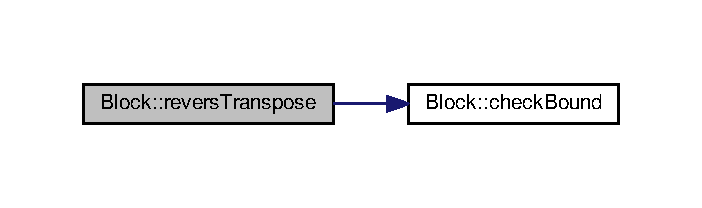
\includegraphics[width=337pt]{class_block_a18bfe78145650d1b13267000feea278b_cgraph}
\end{center}
\end{figure}




이 함수를 호출하는 함수들에 대한 그래프입니다.\+:
\nopagebreak
\begin{figure}[H]
\begin{center}
\leavevmode
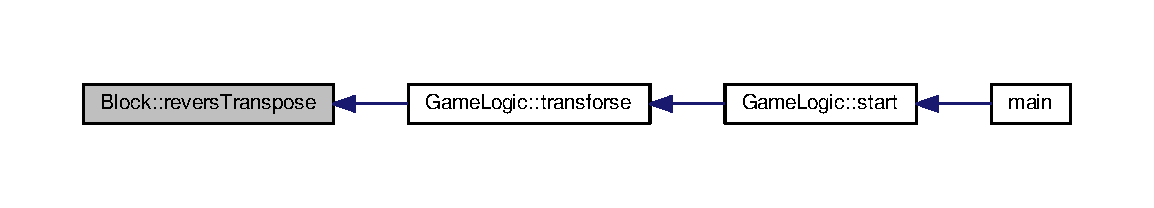
\includegraphics[width=350pt]{class_block_a18bfe78145650d1b13267000feea278b_icgraph}
\end{center}
\end{figure}


\index{Block@{Block}!transpose@{transpose}}
\index{transpose@{transpose}!Block@{Block}}
\subsubsection[{\texorpdfstring{transpose()}{transpose()}}]{\setlength{\rightskip}{0pt plus 5cm}void Block\+::transpose (
\begin{DoxyParamCaption}
{}
\end{DoxyParamCaption}
)}\hypertarget{class_block_a9cc446ec51a125982c41e67af63059b0}{}\label{class_block_a9cc446ec51a125982c41e67af63059b0}


Block.\+cpp 파일의 136 번째 라인에서 정의되었습니다.


\begin{DoxyCode}
136                       \{
137     \textcolor{keywordtype}{int} s = \hyperlink{class_block_a11fa34418f20b6613d0ceeea8fc71d25}{color} - 41;
138     \hyperlink{class_block_a786c39534d84f71238f0189d8852e432}{stat} = (\hyperlink{class_block_a786c39534d84f71238f0189d8852e432}{stat} + 1) % 4;
139     \hyperlink{class_block_ae1a4e97236e1e5f04d21fc9227b8c3a8}{shape}[0] = \hyperlink{class_block_a87730d80e01cf50689abc8525d27f06d}{Block::block\_shape}[s][\hyperlink{class_block_a786c39534d84f71238f0189d8852e432}{stat}][0];
140     \hyperlink{class_block_ae1a4e97236e1e5f04d21fc9227b8c3a8}{shape}[1] = \hyperlink{class_block_a87730d80e01cf50689abc8525d27f06d}{Block::block\_shape}[s][\hyperlink{class_block_a786c39534d84f71238f0189d8852e432}{stat}][1];
141     \hyperlink{class_block_ae1a4e97236e1e5f04d21fc9227b8c3a8}{shape}[2] = \hyperlink{class_block_a87730d80e01cf50689abc8525d27f06d}{Block::block\_shape}[s][\hyperlink{class_block_a786c39534d84f71238f0189d8852e432}{stat}][2];
142     \hyperlink{class_block_ae1a4e97236e1e5f04d21fc9227b8c3a8}{shape}[3] = \hyperlink{class_block_a87730d80e01cf50689abc8525d27f06d}{Block::block\_shape}[s][\hyperlink{class_block_a786c39534d84f71238f0189d8852e432}{stat}][3];
143     \hyperlink{class_block_a4ce6f20dfa2c216f77cbc1a7f2a6f3a2}{checkBound}();
144 \}
\end{DoxyCode}


이 함수 내부에서 호출하는 함수들에 대한 그래프입니다.\+:
\nopagebreak
\begin{figure}[H]
\begin{center}
\leavevmode
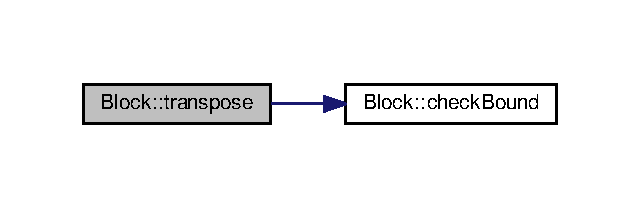
\includegraphics[width=307pt]{class_block_a9cc446ec51a125982c41e67af63059b0_cgraph}
\end{center}
\end{figure}




이 함수를 호출하는 함수들에 대한 그래프입니다.\+:
\nopagebreak
\begin{figure}[H]
\begin{center}
\leavevmode
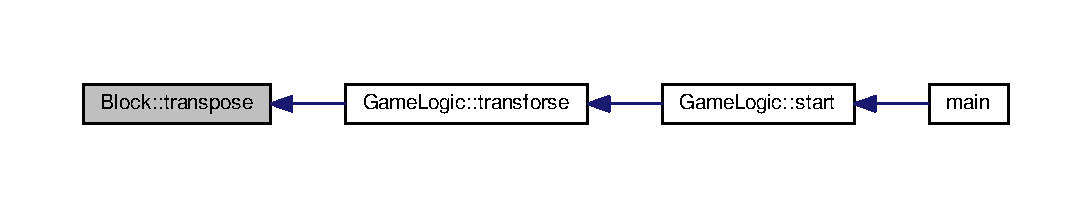
\includegraphics[width=350pt]{class_block_a9cc446ec51a125982c41e67af63059b0_icgraph}
\end{center}
\end{figure}




\subsection{멤버 데이타 문서화}
\index{Block@{Block}!B\+L\+O\+CK@{B\+L\+O\+CK}}
\index{B\+L\+O\+CK@{B\+L\+O\+CK}!Block@{Block}}
\subsubsection[{\texorpdfstring{B\+L\+O\+CK}{BLOCK}}]{\setlength{\rightskip}{0pt plus 5cm}const char $\ast$ Block\+::\+B\+L\+O\+CK = \char`\"{}\mbox{[}$\,$\mbox{]}\char`\"{}\hspace{0.3cm}{\ttfamily [static]}}\hypertarget{class_block_a4cb64c2c20884eed68c24c6147f68514}{}\label{class_block_a4cb64c2c20884eed68c24c6147f68514}
@ brief block shape 

Block.\+h 파일의 22 번째 라인에서 정의되었습니다.

\index{Block@{Block}!block\+\_\+shape@{block\+\_\+shape}}
\index{block\+\_\+shape@{block\+\_\+shape}!Block@{Block}}
\subsubsection[{\texorpdfstring{block\+\_\+shape}{block_shape}}]{\setlength{\rightskip}{0pt plus 5cm}const {\bf Point} Block\+::block\+\_\+shape\hspace{0.3cm}{\ttfamily [static]}, {\ttfamily [private]}}\hypertarget{class_block_a87730d80e01cf50689abc8525d27f06d}{}\label{class_block_a87730d80e01cf50689abc8525d27f06d}


block embody 

work with 3-\/dimensional array

2-\/dimension for block

1-\/dimension for save blocks 

Block.\+h 파일의 17 번째 라인에서 정의되었습니다.

\index{Block@{Block}!B\+O\+T\+T\+OM@{B\+O\+T\+T\+OM}}
\index{B\+O\+T\+T\+OM@{B\+O\+T\+T\+OM}!Block@{Block}}
\subsubsection[{\texorpdfstring{B\+O\+T\+T\+OM}{BOTTOM}}]{\setlength{\rightskip}{0pt plus 5cm}const int Block\+::\+B\+O\+T\+T\+OM ={\bf H\+E\+I\+G\+HT}+1\hspace{0.3cm}{\ttfamily [static]}, {\ttfamily [private]}}\hypertarget{class_block_acae0f4fec218b09fc2ea00e6fa97f9a5}{}\label{class_block_acae0f4fec218b09fc2ea00e6fa97f9a5}


Block.\+h 파일의 16 번째 라인에서 정의되었습니다.

\index{Block@{Block}!bottom@{bottom}}
\index{bottom@{bottom}!Block@{Block}}
\subsubsection[{\texorpdfstring{bottom}{bottom}}]{\setlength{\rightskip}{0pt plus 5cm}int Block\+::bottom}\hypertarget{class_block_a8d97d8b0b6a09592ac007c13c3fa3867}{}\label{class_block_a8d97d8b0b6a09592ac007c13c3fa3867}


Block.\+h 파일의 28 번째 라인에서 정의되었습니다.

\index{Block@{Block}!C\+L\+E\+AR@{C\+L\+E\+AR}}
\index{C\+L\+E\+AR@{C\+L\+E\+AR}!Block@{Block}}
\subsubsection[{\texorpdfstring{C\+L\+E\+AR}{CLEAR}}]{\setlength{\rightskip}{0pt plus 5cm}const char $\ast$ Block\+::\+C\+L\+E\+AR = \char`\"{} \char`\"{}\hspace{0.3cm}{\ttfamily [static]}}\hypertarget{class_block_a11bcda9589b54be35a8905ca7be7310e}{}\label{class_block_a11bcda9589b54be35a8905ca7be7310e}


Block.\+h 파일의 23 번째 라인에서 정의되었습니다.

\index{Block@{Block}!color@{color}}
\index{color@{color}!Block@{Block}}
\subsubsection[{\texorpdfstring{color}{color}}]{\setlength{\rightskip}{0pt plus 5cm}int Block\+::color}\hypertarget{class_block_a11fa34418f20b6613d0ceeea8fc71d25}{}\label{class_block_a11fa34418f20b6613d0ceeea8fc71d25}


Block.\+h 파일의 29 번째 라인에서 정의되었습니다.

\index{Block@{Block}!current@{current}}
\index{current@{current}!Block@{Block}}
\subsubsection[{\texorpdfstring{current}{current}}]{\setlength{\rightskip}{0pt plus 5cm}{\bf Point} Block\+::current}\hypertarget{class_block_aeb5dd312b719966752ba4b38720a4535}{}\label{class_block_aeb5dd312b719966752ba4b38720a4535}


Block.\+h 파일의 25 번째 라인에서 정의되었습니다.

\index{Block@{Block}!L\+E\+FT@{L\+E\+FT}}
\index{L\+E\+FT@{L\+E\+FT}!Block@{Block}}
\subsubsection[{\texorpdfstring{L\+E\+FT}{LEFT}}]{\setlength{\rightskip}{0pt plus 5cm}const int Block\+::\+L\+E\+FT =0\hspace{0.3cm}{\ttfamily [static]}, {\ttfamily [private]}}\hypertarget{class_block_ac5f5e2234205915a274e7aa43a476a62}{}\label{class_block_ac5f5e2234205915a274e7aa43a476a62}


Block.\+h 파일의 16 번째 라인에서 정의되었습니다.

\index{Block@{Block}!left@{left}}
\index{left@{left}!Block@{Block}}
\subsubsection[{\texorpdfstring{left}{left}}]{\setlength{\rightskip}{0pt plus 5cm}int Block\+::left}\hypertarget{class_block_a1e4846853623ef67785a1bae5cec623e}{}\label{class_block_a1e4846853623ef67785a1bae5cec623e}


Block.\+h 파일의 26 번째 라인에서 정의되었습니다.

\index{Block@{Block}!prev@{prev}}
\index{prev@{prev}!Block@{Block}}
\subsubsection[{\texorpdfstring{prev}{prev}}]{\setlength{\rightskip}{0pt plus 5cm}{\bf Point} Block\+::prev\hspace{0.3cm}{\ttfamily [private]}}\hypertarget{class_block_ab86ce4753987a3eb39058553fd81b462}{}\label{class_block_ab86ce4753987a3eb39058553fd81b462}


Block.\+h 파일의 19 번째 라인에서 정의되었습니다.

\index{Block@{Block}!R\+I\+G\+HT@{R\+I\+G\+HT}}
\index{R\+I\+G\+HT@{R\+I\+G\+HT}!Block@{Block}}
\subsubsection[{\texorpdfstring{R\+I\+G\+HT}{RIGHT}}]{\setlength{\rightskip}{0pt plus 5cm}const int Block\+::\+R\+I\+G\+HT ={\bf W\+I\+D\+TH}-\/1\hspace{0.3cm}{\ttfamily [static]}, {\ttfamily [private]}}\hypertarget{class_block_a446deab28dcc4d905bb33219eb6da3dc}{}\label{class_block_a446deab28dcc4d905bb33219eb6da3dc}


Block.\+h 파일의 16 번째 라인에서 정의되었습니다.

\index{Block@{Block}!right@{right}}
\index{right@{right}!Block@{Block}}
\subsubsection[{\texorpdfstring{right}{right}}]{\setlength{\rightskip}{0pt plus 5cm}int Block\+::right}\hypertarget{class_block_a370e4fb56e296b92eb2cc3916b3f39b2}{}\label{class_block_a370e4fb56e296b92eb2cc3916b3f39b2}


Block.\+h 파일의 27 번째 라인에서 정의되었습니다.

\index{Block@{Block}!shape@{shape}}
\index{shape@{shape}!Block@{Block}}
\subsubsection[{\texorpdfstring{shape}{shape}}]{\setlength{\rightskip}{0pt plus 5cm}{\bf Point} Block\+::shape\mbox{[}4\mbox{]}}\hypertarget{class_block_ae1a4e97236e1e5f04d21fc9227b8c3a8}{}\label{class_block_ae1a4e97236e1e5f04d21fc9227b8c3a8}


Block.\+h 파일의 30 번째 라인에서 정의되었습니다.

\index{Block@{Block}!stat@{stat}}
\index{stat@{stat}!Block@{Block}}
\subsubsection[{\texorpdfstring{stat}{stat}}]{\setlength{\rightskip}{0pt plus 5cm}int Block\+::stat\hspace{0.3cm}{\ttfamily [private]}}\hypertarget{class_block_a786c39534d84f71238f0189d8852e432}{}\label{class_block_a786c39534d84f71238f0189d8852e432}


Block.\+h 파일의 18 번째 라인에서 정의되었습니다.

\index{Block@{Block}!T\+OP@{T\+OP}}
\index{T\+OP@{T\+OP}!Block@{Block}}
\subsubsection[{\texorpdfstring{T\+OP}{TOP}}]{\setlength{\rightskip}{0pt plus 5cm}const int Block\+::\+T\+OP =0\hspace{0.3cm}{\ttfamily [static]}, {\ttfamily [private]}}\hypertarget{class_block_a8609875a08b9ec9e07aec1e9ed1e6c7f}{}\label{class_block_a8609875a08b9ec9e07aec1e9ed1e6c7f}


Block.\+h 파일의 16 번째 라인에서 정의되었습니다.

\index{Block@{Block}!zero@{zero}}
\index{zero@{zero}!Block@{Block}}
\subsubsection[{\texorpdfstring{zero}{zero}}]{\setlength{\rightskip}{0pt plus 5cm}{\bf Point} Block\+::zero = {\bf Point}()\hspace{0.3cm}{\ttfamily [static]}}\hypertarget{class_block_ad456f4794a480711f7057e1f270d93c2}{}\label{class_block_ad456f4794a480711f7057e1f270d93c2}


Block.\+h 파일의 24 번째 라인에서 정의되었습니다.



이 클래스에 대한 문서화 페이지는 다음의 파일들로부터 생성되었습니다.\+:\begin{DoxyCompactItemize}
\item 
\hyperlink{_block_8h}{Block.\+h}\item 
\hyperlink{_block_8cpp}{Block.\+cpp}\end{DoxyCompactItemize}

\hypertarget{class_game_logic}{}\section{Game\+Logic 클래스 참조}
\label{class_game_logic}\index{Game\+Logic@{Game\+Logic}}


{\ttfamily \#include $<$Game\+Logic.\+h$>$}



Game\+Logic에 대한 협력 다이어그램\+:
\nopagebreak
\begin{figure}[H]
\begin{center}
\leavevmode
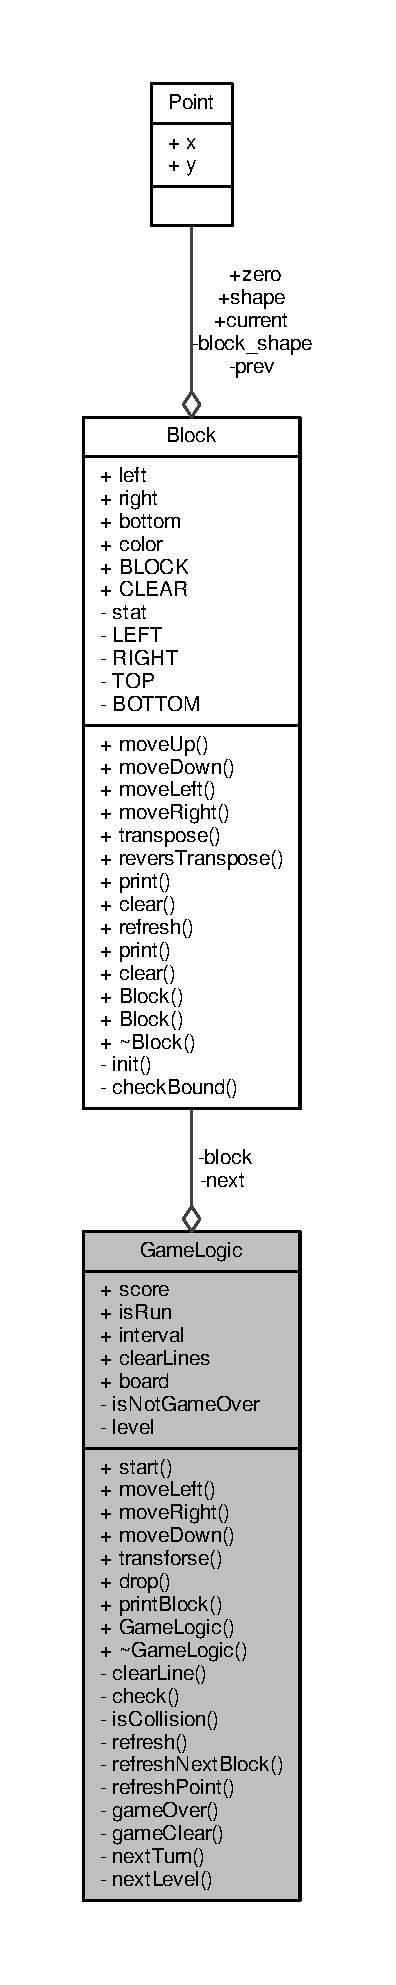
\includegraphics[height=550pt]{class_game_logic__coll__graph}
\end{center}
\end{figure}
\subsection*{Public 멤버 함수}
\begin{DoxyCompactItemize}
\item 
void \hyperlink{class_game_logic_aeb7d3db8014da87a18ac744d9f77131d}{start} ()
\item 
void \hyperlink{class_game_logic_a0e6c1ee03971cf619212f8bb4d5fbc83}{move\+Left} ()
\item 
void \hyperlink{class_game_logic_a6213333800f3aa800ea448ad3ee3ea7c}{move\+Right} ()
\item 
void \hyperlink{class_game_logic_a36b04a5ca335351249db8cc77019c216}{move\+Down} ()
\item 
void \hyperlink{class_game_logic_abd2dece64def6dc89e0b116fdca83483}{transforse} ()
\item 
void \hyperlink{class_game_logic_a90faee03fd4311eab796ae7dc582078d}{drop} ()
\item 
void \hyperlink{class_game_logic_ad0f9f0e6c978a3b3fa1ff7a2a3d92563}{print\+Block} ()
\item 
\hyperlink{class_game_logic_a996cd781691c36922e7ce792fcb21640}{Game\+Logic} ()
\item 
virtual \hyperlink{class_game_logic_a63a7acf778535b5f74d469de2cd39b16}{$\sim$\+Game\+Logic} ()
\end{DoxyCompactItemize}
\subsection*{Public 속성}
\begin{DoxyCompactItemize}
\item 
int \hyperlink{class_game_logic_a64ebe1cc14b91b935608ae4455fe3745}{score}
\item 
bool \hyperlink{class_game_logic_a6a95fb9e16b411f1149dcdb463cdc3a5}{is\+Run}
\item 
int \hyperlink{class_game_logic_ab9459c489b9c7bba90895756f373afc6}{interval}
\item 
int \hyperlink{class_game_logic_ab630a474170a2878d0c5ba8556e3fb39}{clear\+Lines}
\item 
char $\ast$ \hyperlink{class_game_logic_a71071a20595279a580d18dfa60ed4a1c}{board} \mbox{[}\hyperlink{_game_logic_8h_af728b7647e0b8c49832983a31f9a2e9b}{H\+E\+I\+G\+HT}\mbox{]}
\end{DoxyCompactItemize}
\subsection*{Private 멤버 함수}
\begin{DoxyCompactItemize}
\item 
void \hyperlink{class_game_logic_aa94e4cc11eb878caf3b4889e267fd7d7}{clear\+Line} (int line)
\item 
void \hyperlink{class_game_logic_afabf48aab0520a7ecd576bfc178d4767}{check} (\hyperlink{class_block}{Block} \hyperlink{class_game_logic_a499d9b05317bb6a77bf3521f42a6638a}{block})
\item 
bool \hyperlink{class_game_logic_a1c534033fe42c8af4fb0e11e3fed2cfa}{is\+Collision} ()
\item 
void \hyperlink{class_game_logic_aff831622dc54c1737e76b00d0d44ccef}{refresh} ()
\item 
void \hyperlink{class_game_logic_a81fa5e44fb6dc431c926f7c3fd0b7cdb}{refresh\+Next\+Block} ()
\item 
void \hyperlink{class_game_logic_a3f19ca1ad6a1c829afe571f7ac25d3c5}{refresh\+Point} ()
\item 
void \hyperlink{class_game_logic_af6ba400e79f01e5c59f48f55273894e6}{game\+Over} ()
\item 
void \hyperlink{class_game_logic_abf26417f7a1fff03e6639b8bd69490f0}{game\+Clear} ()
\item 
void \hyperlink{class_game_logic_a70b7fcd97d321dfb9d2130f864ddac3b}{next\+Turn} ()
\item 
void \hyperlink{class_game_logic_a5cc64703af4a64975fe24aa5c1d3c711}{next\+Level} ()
\begin{DoxyCompactList}\small\item\em level system \end{DoxyCompactList}\end{DoxyCompactItemize}
\subsection*{Private 속성}
\begin{DoxyCompactItemize}
\item 
\hyperlink{class_block}{Block} \hyperlink{class_game_logic_a499d9b05317bb6a77bf3521f42a6638a}{block}
\item 
\hyperlink{class_block}{Block} \hyperlink{class_game_logic_a42f7be1948bf9cf0a8ff05d7544f62bc}{next}
\item 
bool \hyperlink{class_game_logic_ae09fc4252ad9db62b810117567783880}{is\+Not\+Game\+Over}
\item 
int \hyperlink{class_game_logic_aca26b3a67b4bb5d5d477f9873826aae8}{level}
\end{DoxyCompactItemize}


\subsection{상세한 설명}


Game\+Logic.\+h 파일의 15 번째 라인에서 정의되었습니다.



\subsection{생성자 \& 소멸자 문서화}
\index{Game\+Logic@{Game\+Logic}!Game\+Logic@{Game\+Logic}}
\index{Game\+Logic@{Game\+Logic}!Game\+Logic@{Game\+Logic}}
\subsubsection[{\texorpdfstring{Game\+Logic()}{GameLogic()}}]{\setlength{\rightskip}{0pt plus 5cm}Game\+Logic\+::\+Game\+Logic (
\begin{DoxyParamCaption}
{}
\end{DoxyParamCaption}
)}\hypertarget{class_game_logic_a996cd781691c36922e7ce792fcb21640}{}\label{class_game_logic_a996cd781691c36922e7ce792fcb21640}


Game\+Logic.\+cpp 파일의 19 번째 라인에서 정의되었습니다.


\begin{DoxyCode}
19                      \{
20     \textcolor{keywordflow}{for} (\textcolor{keywordtype}{int} i = 0; i < \hyperlink{_game_logic_8h_af728b7647e0b8c49832983a31f9a2e9b}{HEIGHT} + 1; i++) \{
21         \hyperlink{class_game_logic_a71071a20595279a580d18dfa60ed4a1c}{board}[i] = \textcolor{keyword}{new} \textcolor{keywordtype}{char}[\hyperlink{_game_logic_8h_a9649ab8139c4c2ea5c93625b30d92a05}{WIDTH}];
22         \textcolor{keywordflow}{for} (\textcolor{keywordtype}{int} j = 0; j < \hyperlink{_game_logic_8h_a9649ab8139c4c2ea5c93625b30d92a05}{WIDTH}; j++) \{
23             \hyperlink{class_game_logic_a71071a20595279a580d18dfa60ed4a1c}{board}[i][j] = 0;
24         \}
25     \}
26     \textcolor{keywordflow}{for} (\textcolor{keywordtype}{int} j = 0; j < \hyperlink{_game_logic_8h_a9649ab8139c4c2ea5c93625b30d92a05}{WIDTH}; j++) \{
27         \hyperlink{class_game_logic_a71071a20595279a580d18dfa60ed4a1c}{board}[\hyperlink{_game_logic_8h_af728b7647e0b8c49832983a31f9a2e9b}{HEIGHT}][j] = 1;
28     \}
29 
30     \hyperlink{class_game_logic_a6a95fb9e16b411f1149dcdb463cdc3a5}{isRun} = \textcolor{keyword}{true};
31     \hyperlink{class_block_ad456f4794a480711f7057e1f270d93c2}{Block::zero}.\hyperlink{struct_point_a8c779e11e694b20e0946105a9f5de842}{x} = 6;
32     \hyperlink{class_block_ad456f4794a480711f7057e1f270d93c2}{Block::zero}.\hyperlink{struct_point_a2e1b5fb2b2a83571f5c0bc0f66a73cf7}{y} = 2;
33 \}
\end{DoxyCode}
\index{Game\+Logic@{Game\+Logic}!````~Game\+Logic@{$\sim$\+Game\+Logic}}
\index{````~Game\+Logic@{$\sim$\+Game\+Logic}!Game\+Logic@{Game\+Logic}}
\subsubsection[{\texorpdfstring{$\sim$\+Game\+Logic()}{~GameLogic()}}]{\setlength{\rightskip}{0pt plus 5cm}Game\+Logic\+::$\sim$\+Game\+Logic (
\begin{DoxyParamCaption}
{}
\end{DoxyParamCaption}
)\hspace{0.3cm}{\ttfamily [virtual]}}\hypertarget{class_game_logic_a63a7acf778535b5f74d469de2cd39b16}{}\label{class_game_logic_a63a7acf778535b5f74d469de2cd39b16}
\begin{DoxyRefDesc}{할일}
\item[\hyperlink{todo__todo000002}{할일}]Auto-\/generated destructor stub\end{DoxyRefDesc}


Game\+Logic.\+cpp 파일의 35 번째 라인에서 정의되었습니다.


\begin{DoxyCode}
35                       \{
42     \textcolor{keywordflow}{for} (\textcolor{keywordtype}{int} i = 0; i < \hyperlink{_game_logic_8h_af728b7647e0b8c49832983a31f9a2e9b}{HEIGHT} + 1; i++) \{
43         \textcolor{keyword}{delete} \hyperlink{class_game_logic_a71071a20595279a580d18dfa60ed4a1c}{board}[i];
44     \}
45 \}
\end{DoxyCode}


\subsection{멤버 함수 문서화}
\index{Game\+Logic@{Game\+Logic}!check@{check}}
\index{check@{check}!Game\+Logic@{Game\+Logic}}
\subsubsection[{\texorpdfstring{check(\+Block block)}{check(Block block)}}]{\setlength{\rightskip}{0pt plus 5cm}void Game\+Logic\+::check (
\begin{DoxyParamCaption}
\item[{{\bf Block}}]{block}
\end{DoxyParamCaption}
)\hspace{0.3cm}{\ttfamily [private]}}\hypertarget{class_game_logic_afabf48aab0520a7ecd576bfc178d4767}{}\label{class_game_logic_afabf48aab0520a7ecd576bfc178d4767}
score system

level up if clearline counts over 20

score takes differnce with line\+Count make combo system

Game\+Logic.\+cpp 파일의 225 번째 라인에서 정의되었습니다.


\begin{DoxyCode}
225                                  \{
226 
227     \textcolor{keywordtype}{bool} needClear = \textcolor{keyword}{false};
228     \textcolor{keywordtype}{bool} removeable;
229     \textcolor{keywordtype}{int} lineCount = 0;
230     \textcolor{keywordtype}{int} y = block.\hyperlink{class_block_aeb5dd312b719966752ba4b38720a4535}{current}.\hyperlink{struct_point_a2e1b5fb2b2a83571f5c0bc0f66a73cf7}{y} + block.\hyperlink{class_block_a8d97d8b0b6a09592ac007c13c3fa3867}{bottom};
231 
232     \textcolor{keywordflow}{for} (\textcolor{keywordtype}{int} i = 0; i < 4; i++) \{
233         removeable = \textcolor{keyword}{true};
234         \textcolor{keywordflow}{for} (\textcolor{keywordtype}{int} x = 0; x < \hyperlink{_game_logic_8h_a9649ab8139c4c2ea5c93625b30d92a05}{WIDTH}; x++) \{
235             \textcolor{keywordflow}{if} (!\hyperlink{class_game_logic_a71071a20595279a580d18dfa60ed4a1c}{board}[y][x]) \{
236                 removeable = \textcolor{keyword}{false};
237                 \textcolor{keywordflow}{break};
238             \}
239         \}
240         \textcolor{keywordflow}{if} (removeable) \{
241             \hyperlink{class_game_logic_aa94e4cc11eb878caf3b4889e267fd7d7}{clearLine}(y);
242             needClear = \textcolor{keyword}{true};
243             lineCount++;
244         \} \textcolor{keywordflow}{else} \{
245             y--;
246         \}
247     \}
255     \textcolor{keywordflow}{switch} (lineCount) \{
256     \textcolor{keywordflow}{case} 1:
257         \hyperlink{class_game_logic_a64ebe1cc14b91b935608ae4455fe3745}{score} += 100;
258         \textcolor{keywordflow}{break};
259     \textcolor{keywordflow}{case} 2:
260         \hyperlink{class_game_logic_a64ebe1cc14b91b935608ae4455fe3745}{score} += 300;
261         \textcolor{keywordflow}{break};
262     \textcolor{keywordflow}{case} 3:
263         \hyperlink{class_game_logic_a64ebe1cc14b91b935608ae4455fe3745}{score} += 500;
264         \textcolor{keywordflow}{break};
265     \textcolor{keywordflow}{case} 4:
266         \hyperlink{class_game_logic_a64ebe1cc14b91b935608ae4455fe3745}{score} += 800;
267         \textcolor{keywordflow}{break};
268     \textcolor{keywordflow}{default}:
269         \textcolor{keywordflow}{break};
270     \}
271     \hyperlink{class_game_logic_ab630a474170a2878d0c5ba8556e3fb39}{clearLines} += lineCount;
272     \textcolor{keywordtype}{char} l[4];
273     sprintf(l, \textcolor{stringliteral}{"%d"}, \hyperlink{class_game_logic_ab630a474170a2878d0c5ba8556e3fb39}{clearLines});
274     \hyperlink{myio_8cpp_afce36429cc875312f4476969820ebb51}{printColorString}(40, 15, 0, l);
275     \textcolor{keywordflow}{if} (\hyperlink{class_game_logic_ab630a474170a2878d0c5ba8556e3fb39}{clearLines} >= 20) \{
276         \hyperlink{class_game_logic_a5cc64703af4a64975fe24aa5c1d3c711}{nextLevel}();
277 
278     \}
279     \textcolor{keywordflow}{if} (needClear)
280         \hyperlink{class_game_logic_aff831622dc54c1737e76b00d0d44ccef}{refresh}();
281 
282 \}
\end{DoxyCode}


이 함수 내부에서 호출하는 함수들에 대한 그래프입니다.\+:
\nopagebreak
\begin{figure}[H]
\begin{center}
\leavevmode
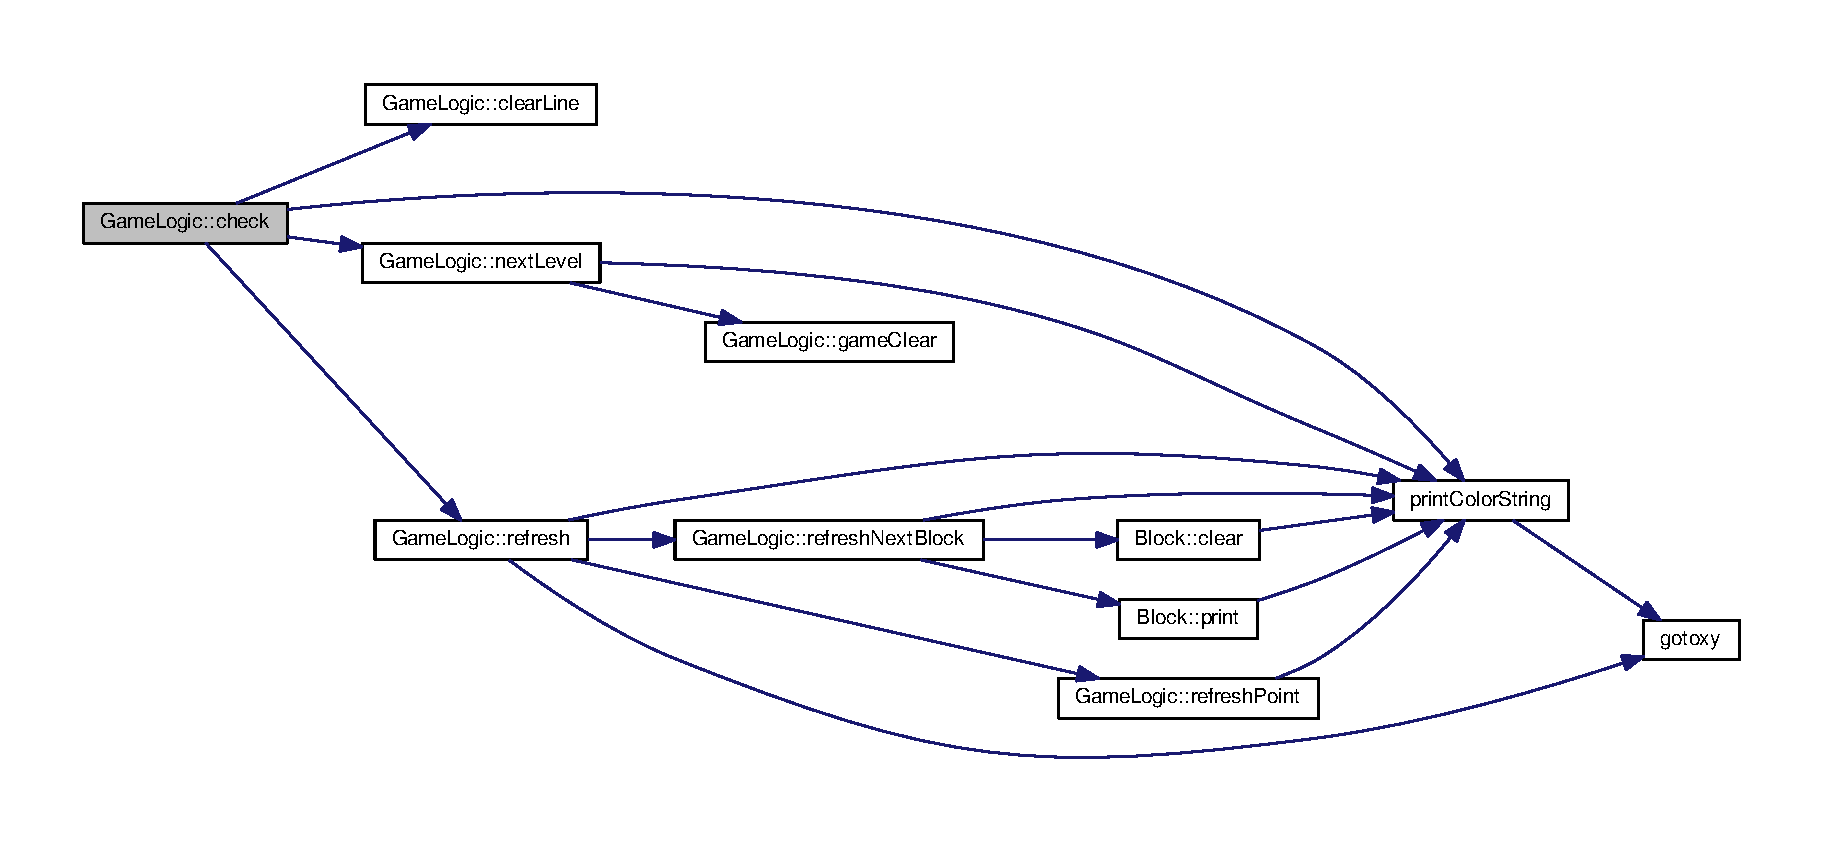
\includegraphics[width=350pt]{class_game_logic_afabf48aab0520a7ecd576bfc178d4767_cgraph}
\end{center}
\end{figure}




이 함수를 호출하는 함수들에 대한 그래프입니다.\+:
\nopagebreak
\begin{figure}[H]
\begin{center}
\leavevmode
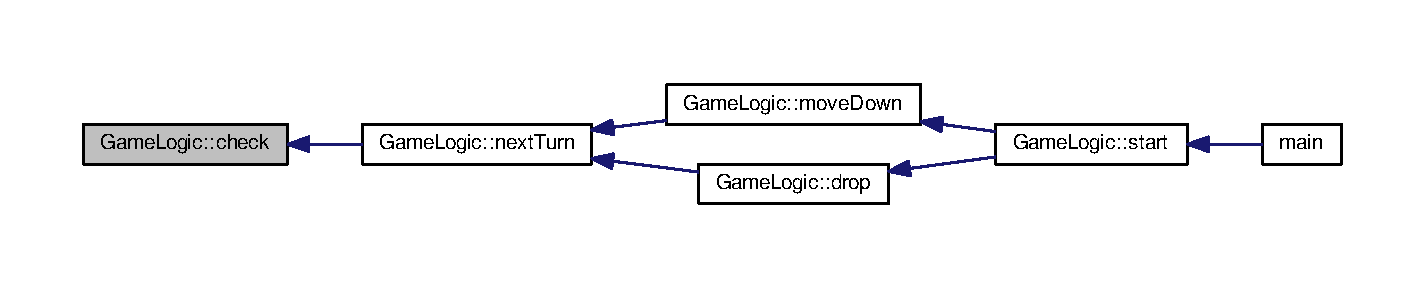
\includegraphics[width=350pt]{class_game_logic_afabf48aab0520a7ecd576bfc178d4767_icgraph}
\end{center}
\end{figure}


\index{Game\+Logic@{Game\+Logic}!clear\+Line@{clear\+Line}}
\index{clear\+Line@{clear\+Line}!Game\+Logic@{Game\+Logic}}
\subsubsection[{\texorpdfstring{clear\+Line(int line)}{clearLine(int line)}}]{\setlength{\rightskip}{0pt plus 5cm}void Game\+Logic\+::clear\+Line (
\begin{DoxyParamCaption}
\item[{int}]{line}
\end{DoxyParamCaption}
)\hspace{0.3cm}{\ttfamily [private]}}\hypertarget{class_game_logic_aa94e4cc11eb878caf3b4889e267fd7d7}{}\label{class_game_logic_aa94e4cc11eb878caf3b4889e267fd7d7}


Game\+Logic.\+cpp 파일의 174 번째 라인에서 정의되었습니다.


\begin{DoxyCode}
174                                \{
175     \textcolor{keywordtype}{char} *line = \hyperlink{class_game_logic_a71071a20595279a580d18dfa60ed4a1c}{board}[l];
176     \textcolor{keywordflow}{for} (\textcolor{keywordtype}{int} y = l; y > 0; y--) \{
177         \hyperlink{class_game_logic_a71071a20595279a580d18dfa60ed4a1c}{board}[y] = \hyperlink{class_game_logic_a71071a20595279a580d18dfa60ed4a1c}{board}[y - 1];
178     \}
179 
180     \hyperlink{class_game_logic_a71071a20595279a580d18dfa60ed4a1c}{board}[0] = line;
181     \textcolor{keywordflow}{for} (\textcolor{keywordtype}{int} x = 0; x < \hyperlink{_game_logic_8h_a9649ab8139c4c2ea5c93625b30d92a05}{WIDTH}; x++) \{
182         \hyperlink{class_game_logic_a71071a20595279a580d18dfa60ed4a1c}{board}[0][x] = 0;
183     \}
184 
185 \}
\end{DoxyCode}


이 함수를 호출하는 함수들에 대한 그래프입니다.\+:
\nopagebreak
\begin{figure}[H]
\begin{center}
\leavevmode
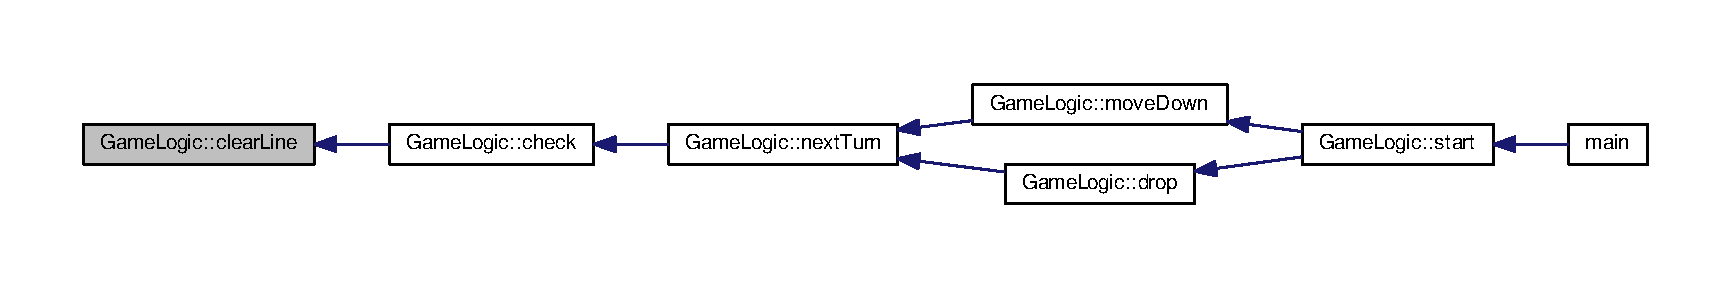
\includegraphics[width=350pt]{class_game_logic_aa94e4cc11eb878caf3b4889e267fd7d7_icgraph}
\end{center}
\end{figure}


\index{Game\+Logic@{Game\+Logic}!drop@{drop}}
\index{drop@{drop}!Game\+Logic@{Game\+Logic}}
\subsubsection[{\texorpdfstring{drop()}{drop()}}]{\setlength{\rightskip}{0pt plus 5cm}void Game\+Logic\+::drop (
\begin{DoxyParamCaption}
{}
\end{DoxyParamCaption}
)}\hypertarget{class_game_logic_a90faee03fd4311eab796ae7dc582078d}{}\label{class_game_logic_a90faee03fd4311eab796ae7dc582078d}


Game\+Logic.\+cpp 파일의 147 번째 라인에서 정의되었습니다.


\begin{DoxyCode}
147                      \{
148 
149     \textcolor{keywordflow}{while} (!\hyperlink{class_game_logic_a1c534033fe42c8af4fb0e11e3fed2cfa}{isCollision}())
150         \hyperlink{class_game_logic_a499d9b05317bb6a77bf3521f42a6638a}{block}.\hyperlink{class_block_a947d677f5229eabb9ceb291e3552773d}{moveDown}();
151 
152     \hyperlink{class_game_logic_a499d9b05317bb6a77bf3521f42a6638a}{block}.\hyperlink{class_block_a8bf4fce7b2b837fd49726b6a7f17f4b0}{moveUp}();
153 
154     \hyperlink{class_game_logic_a70b7fcd97d321dfb9d2130f864ddac3b}{nextTurn}();
155 \}
\end{DoxyCode}


이 함수 내부에서 호출하는 함수들에 대한 그래프입니다.\+:
\nopagebreak
\begin{figure}[H]
\begin{center}
\leavevmode
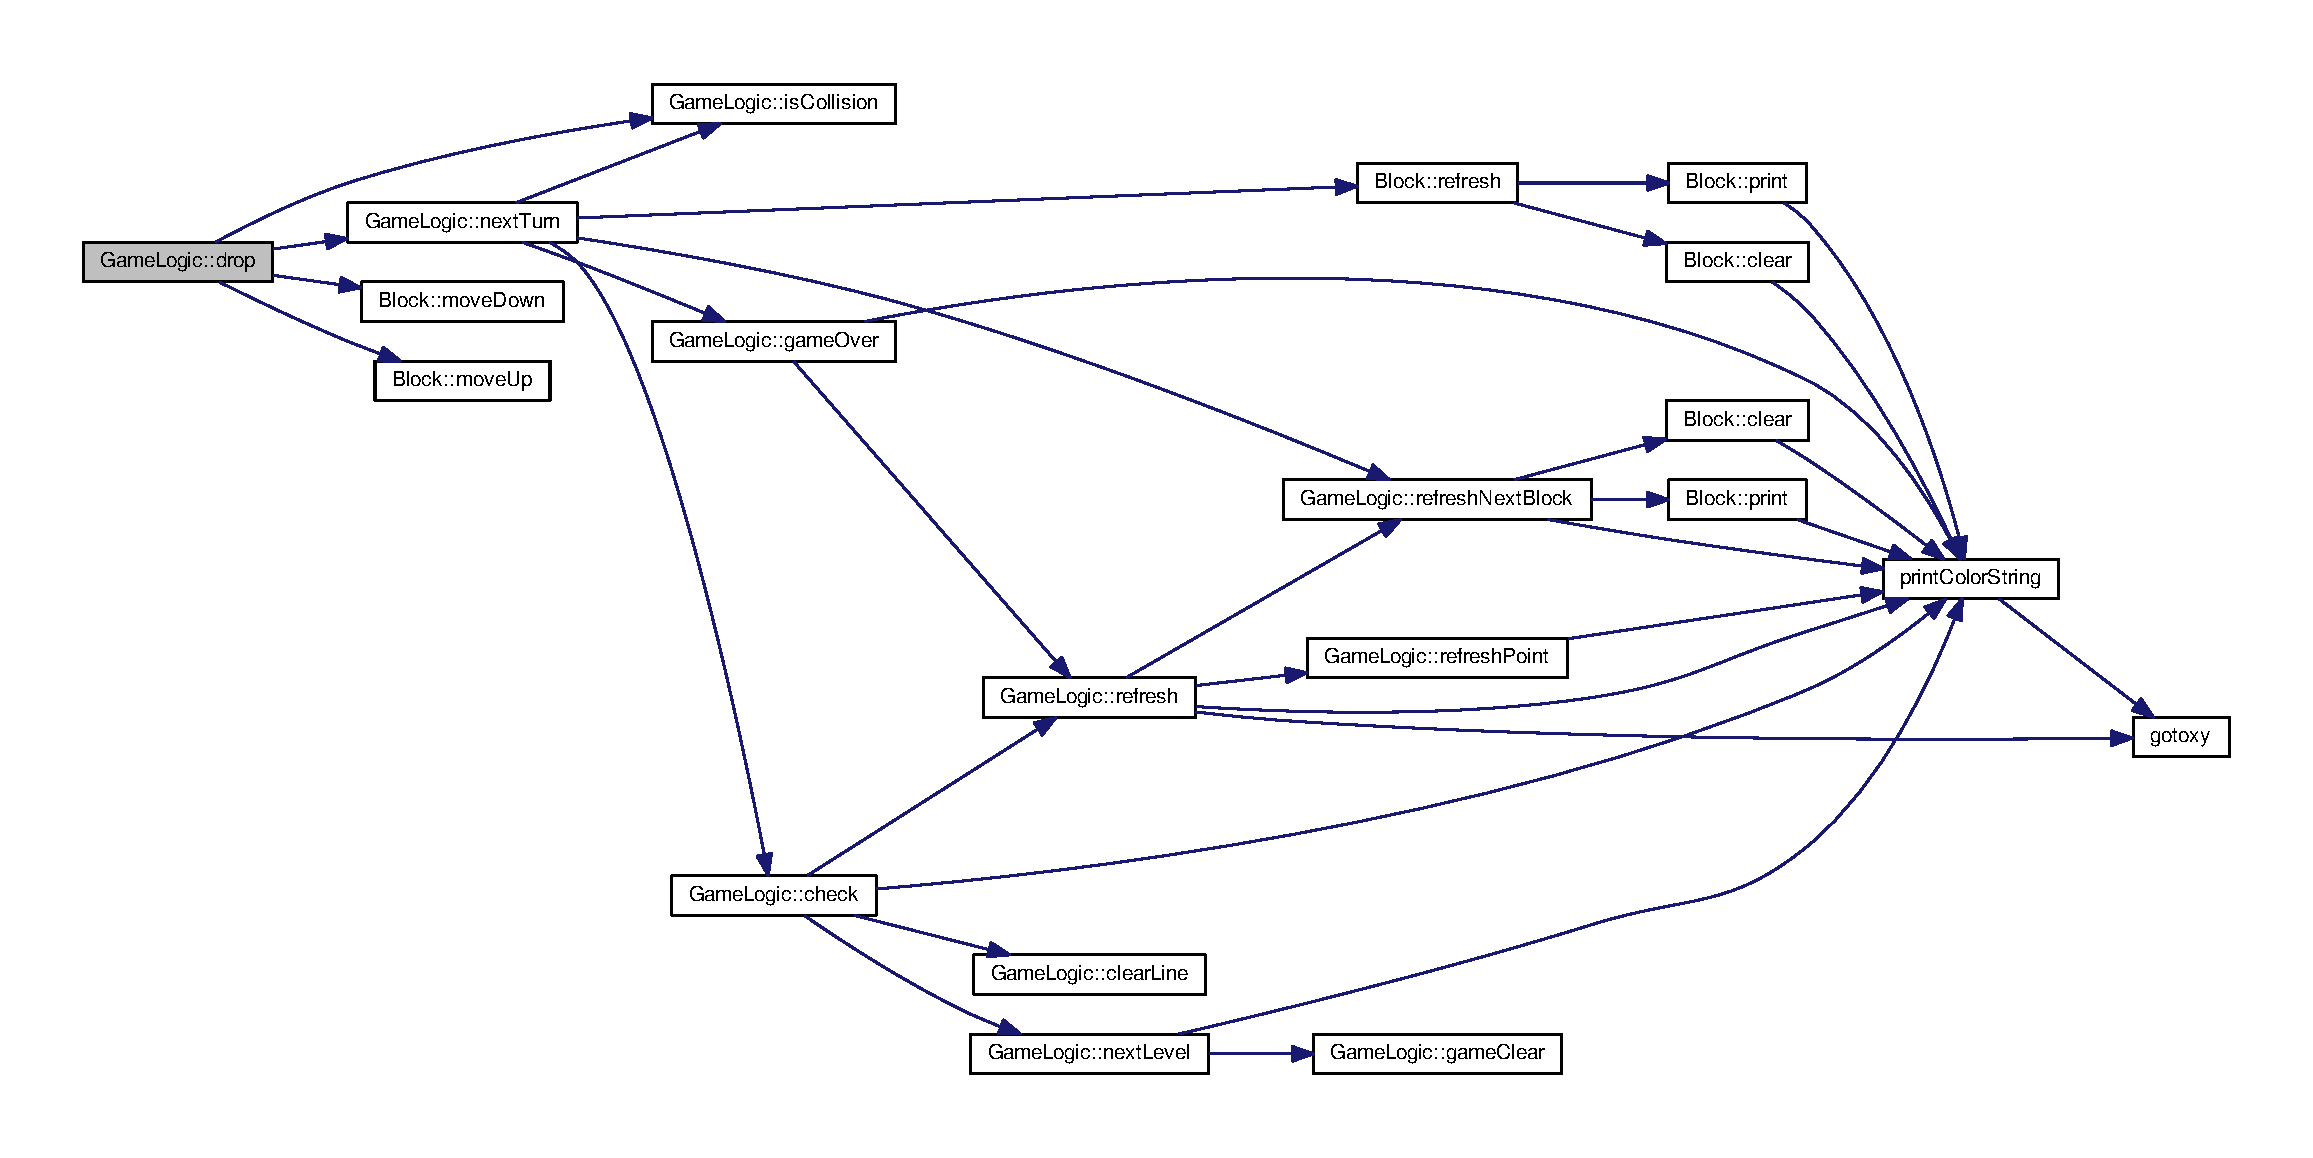
\includegraphics[width=350pt]{class_game_logic_a90faee03fd4311eab796ae7dc582078d_cgraph}
\end{center}
\end{figure}




이 함수를 호출하는 함수들에 대한 그래프입니다.\+:
\nopagebreak
\begin{figure}[H]
\begin{center}
\leavevmode
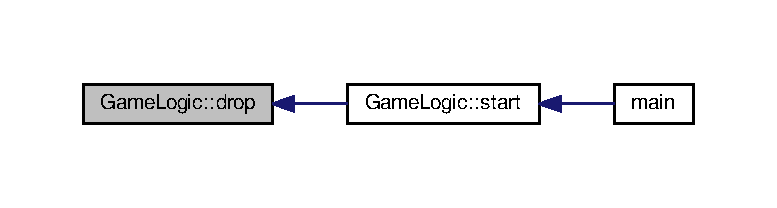
\includegraphics[width=350pt]{class_game_logic_a90faee03fd4311eab796ae7dc582078d_icgraph}
\end{center}
\end{figure}


\index{Game\+Logic@{Game\+Logic}!game\+Clear@{game\+Clear}}
\index{game\+Clear@{game\+Clear}!Game\+Logic@{Game\+Logic}}
\subsubsection[{\texorpdfstring{game\+Clear()}{gameClear()}}]{\setlength{\rightskip}{0pt plus 5cm}void Game\+Logic\+::game\+Clear (
\begin{DoxyParamCaption}
{}
\end{DoxyParamCaption}
)\hspace{0.3cm}{\ttfamily [private]}}\hypertarget{class_game_logic_abf26417f7a1fff03e6639b8bd69490f0}{}\label{class_game_logic_abf26417f7a1fff03e6639b8bd69490f0}


Game\+Logic.\+cpp 파일의 198 번째 라인에서 정의되었습니다.


\begin{DoxyCode}
198                           \{
199 
200 \}
\end{DoxyCode}


이 함수를 호출하는 함수들에 대한 그래프입니다.\+:
\nopagebreak
\begin{figure}[H]
\begin{center}
\leavevmode
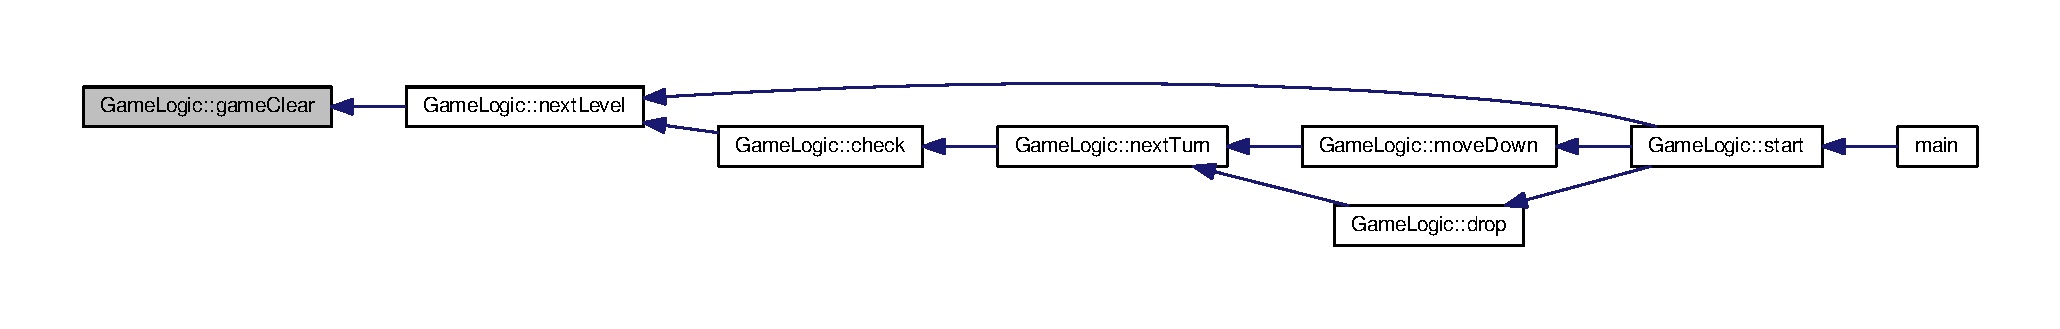
\includegraphics[width=350pt]{class_game_logic_abf26417f7a1fff03e6639b8bd69490f0_icgraph}
\end{center}
\end{figure}


\index{Game\+Logic@{Game\+Logic}!game\+Over@{game\+Over}}
\index{game\+Over@{game\+Over}!Game\+Logic@{Game\+Logic}}
\subsubsection[{\texorpdfstring{game\+Over()}{gameOver()}}]{\setlength{\rightskip}{0pt plus 5cm}void Game\+Logic\+::game\+Over (
\begin{DoxyParamCaption}
{}
\end{DoxyParamCaption}
)\hspace{0.3cm}{\ttfamily [private]}}\hypertarget{class_game_logic_af6ba400e79f01e5c59f48f55273894e6}{}\label{class_game_logic_af6ba400e79f01e5c59f48f55273894e6}


Game\+Logic.\+cpp 파일의 186 번째 라인에서 정의되었습니다.


\begin{DoxyCode}
186                          \{
187     \textcolor{keywordflow}{for} (\textcolor{keywordtype}{int} x = 0; x < \hyperlink{_game_logic_8h_a9649ab8139c4c2ea5c93625b30d92a05}{WIDTH}; x++) \{
188         \textcolor{keywordflow}{for} (\textcolor{keywordtype}{int} y = 0; y < \hyperlink{_game_logic_8h_af728b7647e0b8c49832983a31f9a2e9b}{HEIGHT}; y++) \{
189             \hyperlink{class_game_logic_a71071a20595279a580d18dfa60ed4a1c}{board}[y][x] = 0;
190         \}
191     \}
192     \hyperlink{class_game_logic_aff831622dc54c1737e76b00d0d44ccef}{refresh}();
193     
194     \hyperlink{myio_8cpp_afce36429cc875312f4476969820ebb51}{printColorString}(\hyperlink{class_block_ad456f4794a480711f7057e1f270d93c2}{Block::zero}.x, \hyperlink{class_block_ad456f4794a480711f7057e1f270d93c2}{Block::zero}.y + 10, 
      \hyperlink{myio_8h_aba2a7fe77a7501e5844370eec0185207}{COLOR\_BLACK}, \textcolor{stringliteral}{"gameover"});
195     \hyperlink{class_game_logic_ae09fc4252ad9db62b810117567783880}{isNotGameOver}=\textcolor{keyword}{false};
196 
197 \}
\end{DoxyCode}


이 함수 내부에서 호출하는 함수들에 대한 그래프입니다.\+:
\nopagebreak
\begin{figure}[H]
\begin{center}
\leavevmode
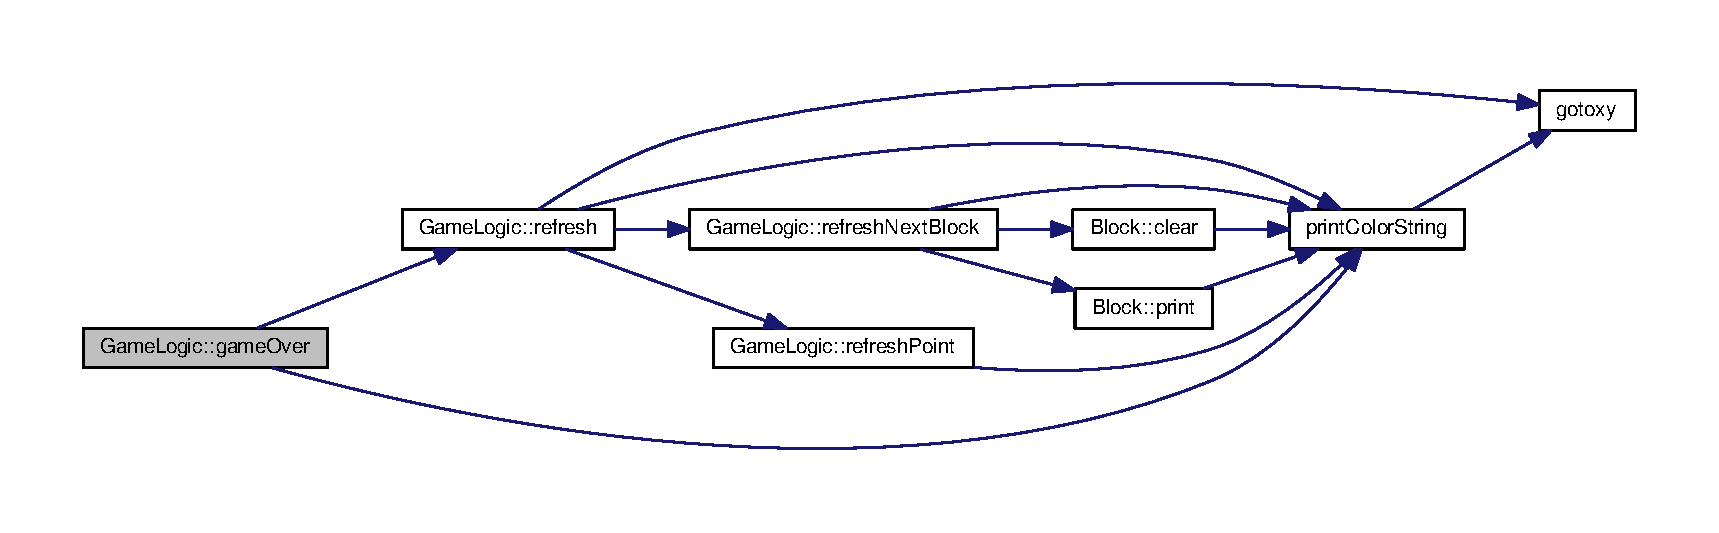
\includegraphics[width=350pt]{class_game_logic_af6ba400e79f01e5c59f48f55273894e6_cgraph}
\end{center}
\end{figure}




이 함수를 호출하는 함수들에 대한 그래프입니다.\+:
\nopagebreak
\begin{figure}[H]
\begin{center}
\leavevmode
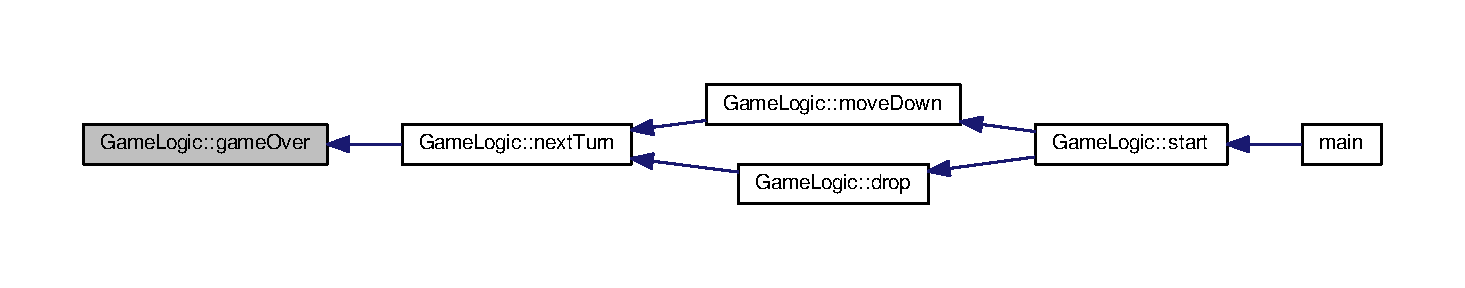
\includegraphics[width=350pt]{class_game_logic_af6ba400e79f01e5c59f48f55273894e6_icgraph}
\end{center}
\end{figure}


\index{Game\+Logic@{Game\+Logic}!is\+Collision@{is\+Collision}}
\index{is\+Collision@{is\+Collision}!Game\+Logic@{Game\+Logic}}
\subsubsection[{\texorpdfstring{is\+Collision()}{isCollision()}}]{\setlength{\rightskip}{0pt plus 5cm}bool Game\+Logic\+::is\+Collision (
\begin{DoxyParamCaption}
{}
\end{DoxyParamCaption}
)\hspace{0.3cm}{\ttfamily [private]}}\hypertarget{class_game_logic_a1c534033fe42c8af4fb0e11e3fed2cfa}{}\label{class_game_logic_a1c534033fe42c8af4fb0e11e3fed2cfa}


Game\+Logic.\+cpp 파일의 157 번째 라인에서 정의되었습니다.


\begin{DoxyCode}
157                             \{
158     \textcolor{keywordtype}{int} x, y;
159     \textcolor{keywordflow}{for} (\textcolor{keywordtype}{int} i = 0; i < 4; i++) \{
160         x = \hyperlink{class_game_logic_a499d9b05317bb6a77bf3521f42a6638a}{block}.\hyperlink{class_block_aeb5dd312b719966752ba4b38720a4535}{current}.\hyperlink{struct_point_a8c779e11e694b20e0946105a9f5de842}{x} + \hyperlink{class_game_logic_a499d9b05317bb6a77bf3521f42a6638a}{block}.\hyperlink{class_block_ae1a4e97236e1e5f04d21fc9227b8c3a8}{shape}[i].\hyperlink{struct_point_a8c779e11e694b20e0946105a9f5de842}{x};
161         y = \hyperlink{class_game_logic_a499d9b05317bb6a77bf3521f42a6638a}{block}.\hyperlink{class_block_aeb5dd312b719966752ba4b38720a4535}{current}.\hyperlink{struct_point_a2e1b5fb2b2a83571f5c0bc0f66a73cf7}{y} + \hyperlink{class_game_logic_a499d9b05317bb6a77bf3521f42a6638a}{block}.\hyperlink{class_block_ae1a4e97236e1e5f04d21fc9227b8c3a8}{shape}[i].\hyperlink{struct_point_a2e1b5fb2b2a83571f5c0bc0f66a73cf7}{y};
162 
163         \textcolor{keywordflow}{if} (x >= \hyperlink{_game_logic_8h_a9649ab8139c4c2ea5c93625b30d92a05}{WIDTH} || y > \hyperlink{_game_logic_8h_af728b7647e0b8c49832983a31f9a2e9b}{HEIGHT} || x < 0) \{
164             \textcolor{keywordflow}{return} \textcolor{keyword}{true};
165         \}
166 
167         \textcolor{keywordflow}{if} (\hyperlink{class_game_logic_a71071a20595279a580d18dfa60ed4a1c}{board}[y][x]) \{
168             \textcolor{keywordflow}{return} \textcolor{keyword}{true};
169         \}
170     \}
171     \textcolor{keywordflow}{return} \textcolor{keyword}{false};
172 \}
\end{DoxyCode}


이 함수를 호출하는 함수들에 대한 그래프입니다.\+:
\nopagebreak
\begin{figure}[H]
\begin{center}
\leavevmode
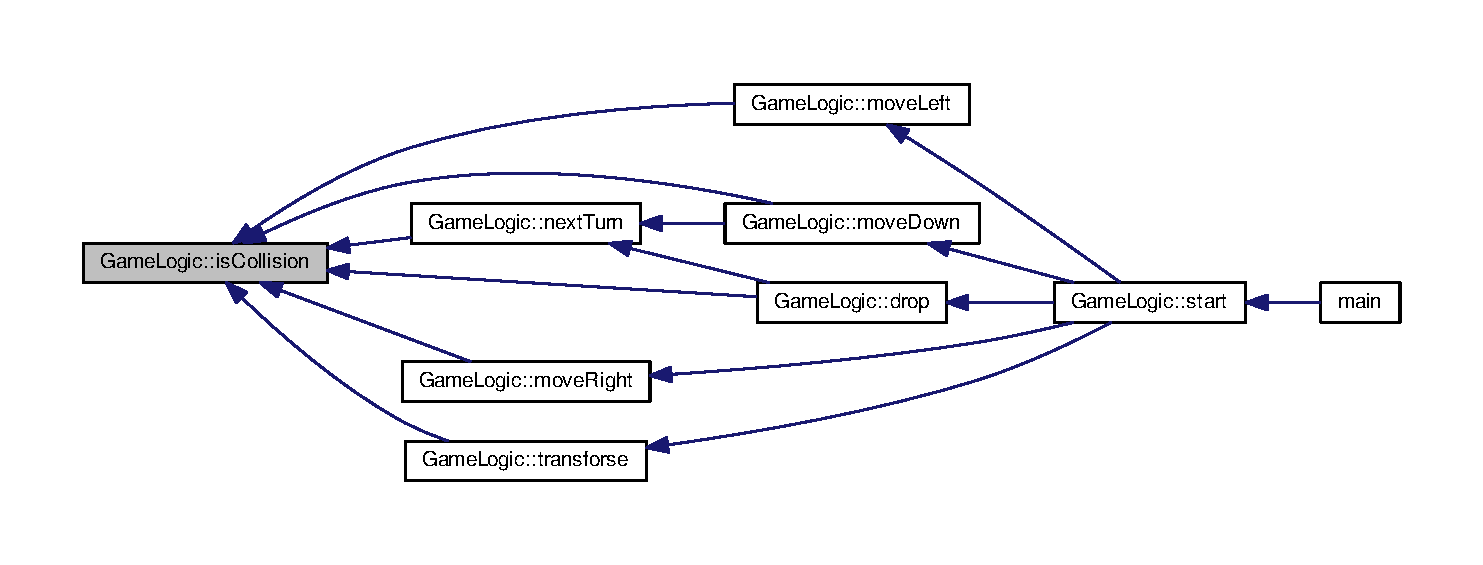
\includegraphics[width=350pt]{class_game_logic_a1c534033fe42c8af4fb0e11e3fed2cfa_icgraph}
\end{center}
\end{figure}


\index{Game\+Logic@{Game\+Logic}!move\+Down@{move\+Down}}
\index{move\+Down@{move\+Down}!Game\+Logic@{Game\+Logic}}
\subsubsection[{\texorpdfstring{move\+Down()}{moveDown()}}]{\setlength{\rightskip}{0pt plus 5cm}void Game\+Logic\+::move\+Down (
\begin{DoxyParamCaption}
{}
\end{DoxyParamCaption}
)}\hypertarget{class_game_logic_a36b04a5ca335351249db8cc77019c216}{}\label{class_game_logic_a36b04a5ca335351249db8cc77019c216}
보드에 저장

Game\+Logic.\+cpp 파일의 107 번째 라인에서 정의되었습니다.


\begin{DoxyCode}
107                          \{
108     \hyperlink{class_game_logic_a499d9b05317bb6a77bf3521f42a6638a}{block}.\hyperlink{class_block_a947d677f5229eabb9ceb291e3552773d}{moveDown}();
109     \textcolor{keywordflow}{if} (\hyperlink{class_game_logic_a1c534033fe42c8af4fb0e11e3fed2cfa}{isCollision}()) \{
110         \hyperlink{class_game_logic_a499d9b05317bb6a77bf3521f42a6638a}{block}.\hyperlink{class_block_a8bf4fce7b2b837fd49726b6a7f17f4b0}{moveUp}();
117         \textcolor{keywordflow}{for} (\textcolor{keywordtype}{int} i = 0; i < 4; i++) \{
118             \hyperlink{class_game_logic_a71071a20595279a580d18dfa60ed4a1c}{board}[\hyperlink{class_game_logic_a499d9b05317bb6a77bf3521f42a6638a}{block}.\hyperlink{class_block_aeb5dd312b719966752ba4b38720a4535}{current}.\hyperlink{struct_point_a2e1b5fb2b2a83571f5c0bc0f66a73cf7}{y} + \hyperlink{class_game_logic_a499d9b05317bb6a77bf3521f42a6638a}{block}.\hyperlink{class_block_ae1a4e97236e1e5f04d21fc9227b8c3a8}{shape}[i].\hyperlink{struct_point_a2e1b5fb2b2a83571f5c0bc0f66a73cf7}{y}][
      \hyperlink{class_game_logic_a499d9b05317bb6a77bf3521f42a6638a}{block}.\hyperlink{class_block_aeb5dd312b719966752ba4b38720a4535}{current}.\hyperlink{struct_point_a8c779e11e694b20e0946105a9f5de842}{x} + \hyperlink{class_game_logic_a499d9b05317bb6a77bf3521f42a6638a}{block}.\hyperlink{class_block_ae1a4e97236e1e5f04d21fc9227b8c3a8}{shape}[i].\hyperlink{struct_point_a8c779e11e694b20e0946105a9f5de842}{x}] = \hyperlink{class_game_logic_a499d9b05317bb6a77bf3521f42a6638a}{block}.\hyperlink{class_block_a11fa34418f20b6613d0ceeea8fc71d25}{color};
119         \}
120         \hyperlink{class_game_logic_a70b7fcd97d321dfb9d2130f864ddac3b}{nextTurn}();
121     \}
122 
123 \}
\end{DoxyCode}


이 함수 내부에서 호출하는 함수들에 대한 그래프입니다.\+:
\nopagebreak
\begin{figure}[H]
\begin{center}
\leavevmode
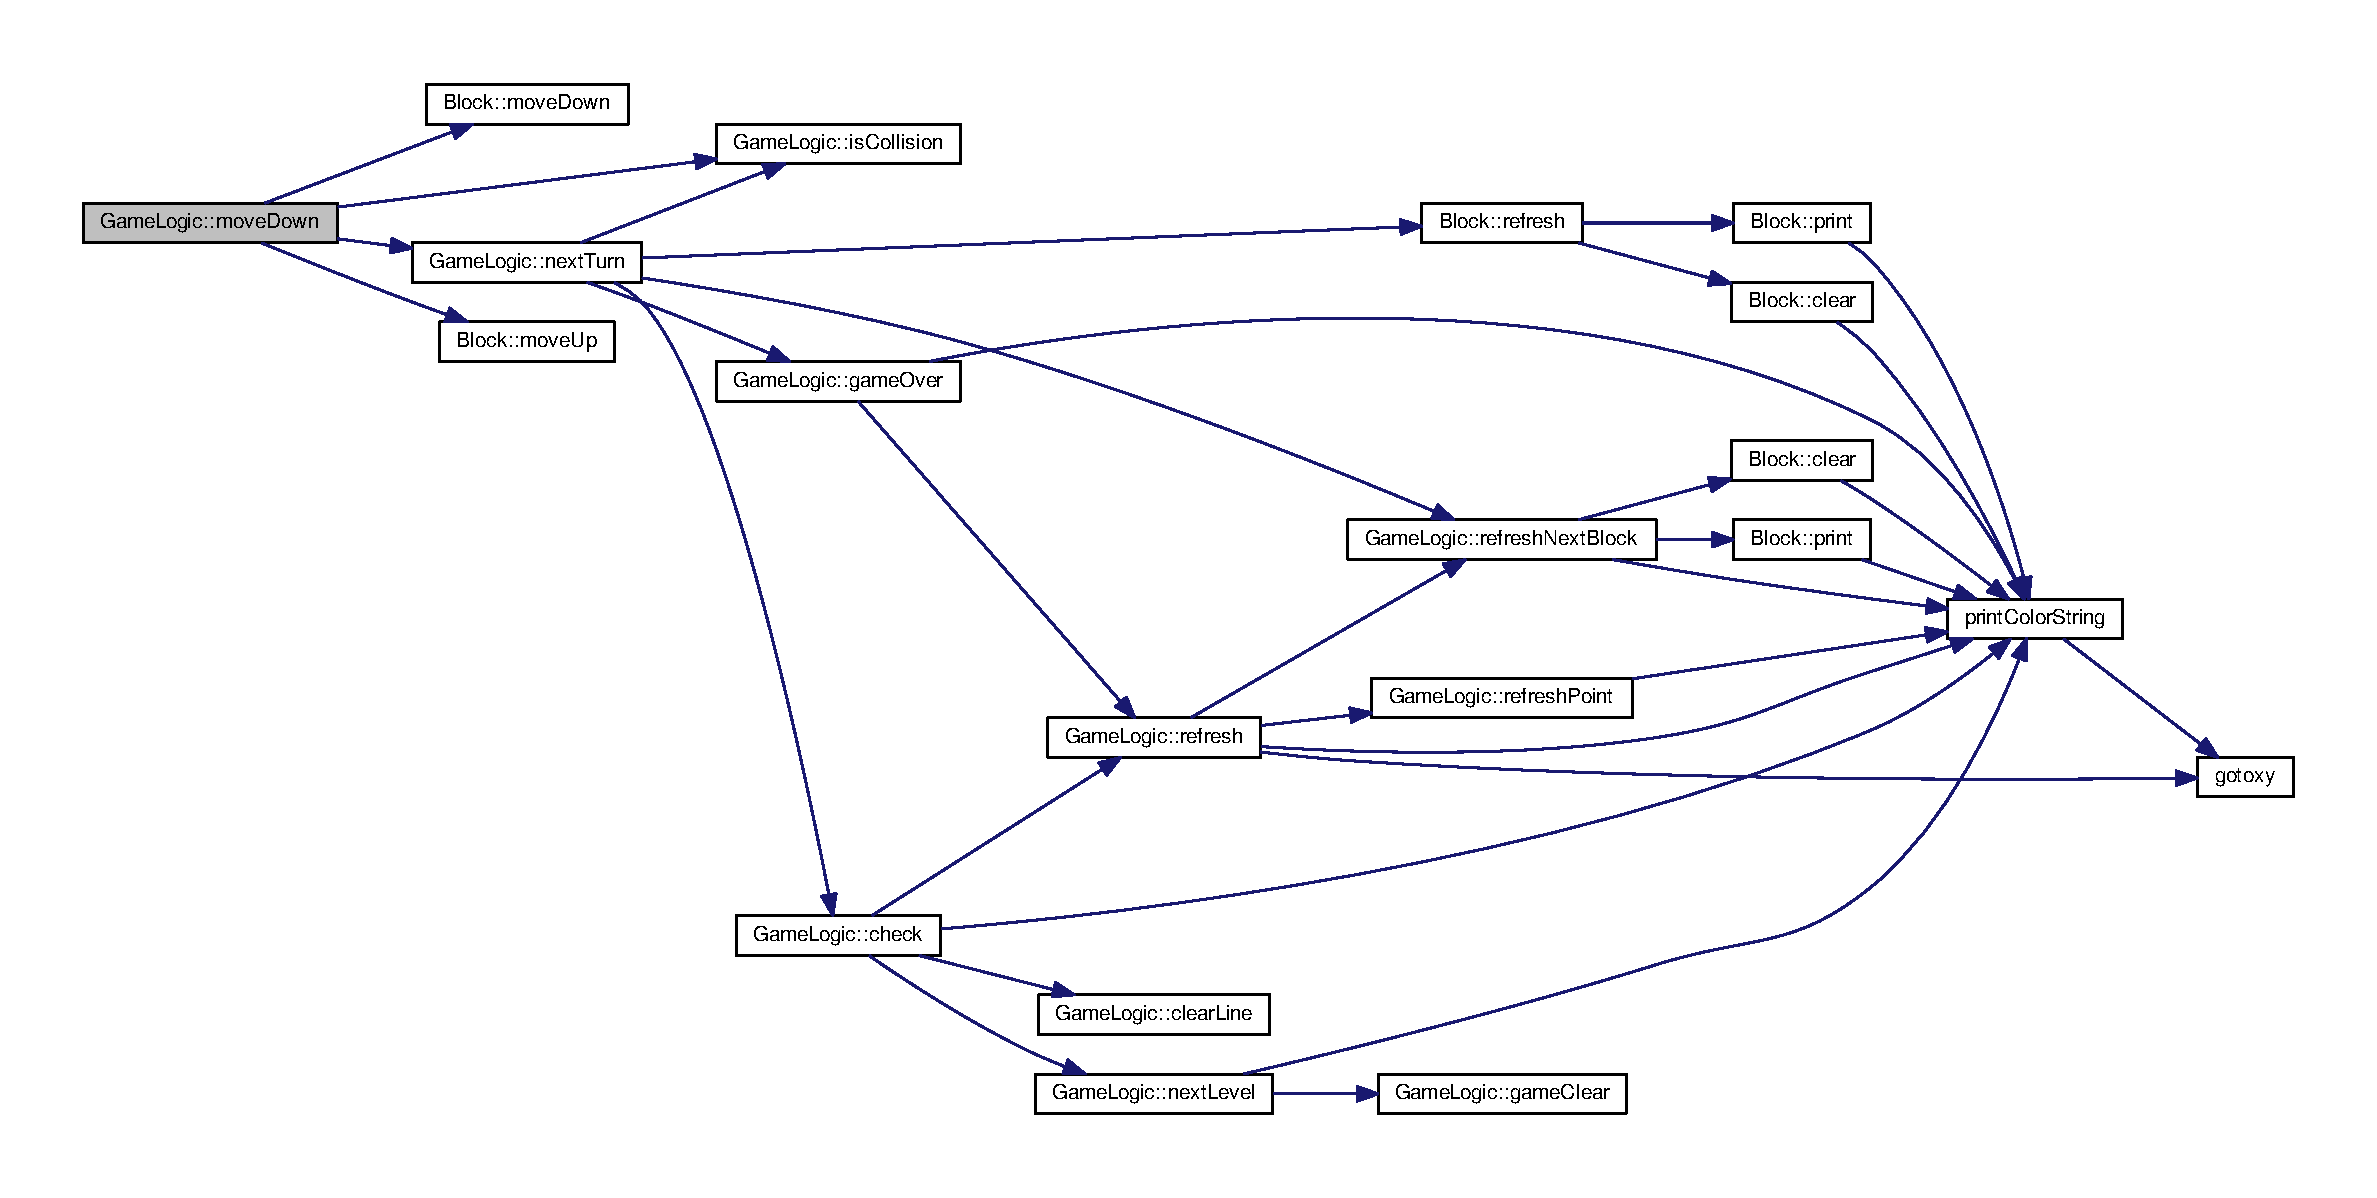
\includegraphics[width=350pt]{class_game_logic_a36b04a5ca335351249db8cc77019c216_cgraph}
\end{center}
\end{figure}




이 함수를 호출하는 함수들에 대한 그래프입니다.\+:
\nopagebreak
\begin{figure}[H]
\begin{center}
\leavevmode
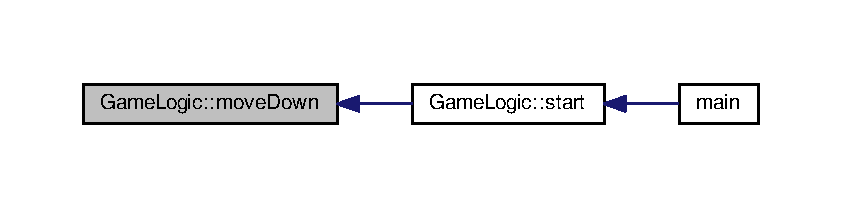
\includegraphics[width=350pt]{class_game_logic_a36b04a5ca335351249db8cc77019c216_icgraph}
\end{center}
\end{figure}


\index{Game\+Logic@{Game\+Logic}!move\+Left@{move\+Left}}
\index{move\+Left@{move\+Left}!Game\+Logic@{Game\+Logic}}
\subsubsection[{\texorpdfstring{move\+Left()}{moveLeft()}}]{\setlength{\rightskip}{0pt plus 5cm}void Game\+Logic\+::move\+Left (
\begin{DoxyParamCaption}
{}
\end{DoxyParamCaption}
)}\hypertarget{class_game_logic_a0e6c1ee03971cf619212f8bb4d5fbc83}{}\label{class_game_logic_a0e6c1ee03971cf619212f8bb4d5fbc83}


Game\+Logic.\+cpp 파일의 124 번째 라인에서 정의되었습니다.


\begin{DoxyCode}
124                          \{
125     \hyperlink{class_game_logic_a499d9b05317bb6a77bf3521f42a6638a}{block}.\hyperlink{class_block_af304df3662f2c6feec7cfc232246ef29}{moveLeft}();
126     \textcolor{keywordflow}{if} (\hyperlink{class_game_logic_a1c534033fe42c8af4fb0e11e3fed2cfa}{isCollision}())
127         \hyperlink{class_game_logic_a499d9b05317bb6a77bf3521f42a6638a}{block}.\hyperlink{class_block_a13d1f87524fed8d686a4d478e41d5096}{moveRight}();
128 \}
\end{DoxyCode}


이 함수 내부에서 호출하는 함수들에 대한 그래프입니다.\+:
\nopagebreak
\begin{figure}[H]
\begin{center}
\leavevmode
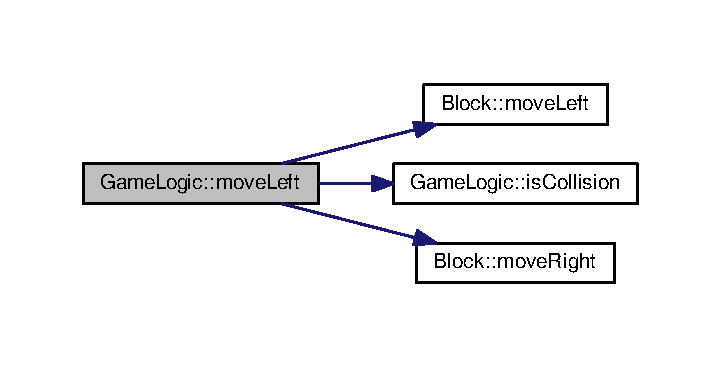
\includegraphics[width=346pt]{class_game_logic_a0e6c1ee03971cf619212f8bb4d5fbc83_cgraph}
\end{center}
\end{figure}




이 함수를 호출하는 함수들에 대한 그래프입니다.\+:
\nopagebreak
\begin{figure}[H]
\begin{center}
\leavevmode
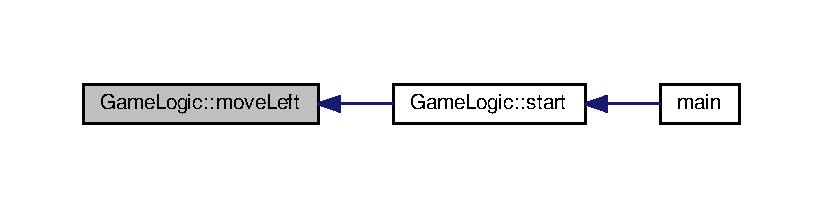
\includegraphics[width=350pt]{class_game_logic_a0e6c1ee03971cf619212f8bb4d5fbc83_icgraph}
\end{center}
\end{figure}


\index{Game\+Logic@{Game\+Logic}!move\+Right@{move\+Right}}
\index{move\+Right@{move\+Right}!Game\+Logic@{Game\+Logic}}
\subsubsection[{\texorpdfstring{move\+Right()}{moveRight()}}]{\setlength{\rightskip}{0pt plus 5cm}void Game\+Logic\+::move\+Right (
\begin{DoxyParamCaption}
{}
\end{DoxyParamCaption}
)}\hypertarget{class_game_logic_a6213333800f3aa800ea448ad3ee3ea7c}{}\label{class_game_logic_a6213333800f3aa800ea448ad3ee3ea7c}


Game\+Logic.\+cpp 파일의 130 번째 라인에서 정의되었습니다.


\begin{DoxyCode}
130                           \{
131     \hyperlink{class_game_logic_a499d9b05317bb6a77bf3521f42a6638a}{block}.\hyperlink{class_block_a13d1f87524fed8d686a4d478e41d5096}{moveRight}();
132     \textcolor{keywordflow}{if} (\hyperlink{class_game_logic_a1c534033fe42c8af4fb0e11e3fed2cfa}{isCollision}())
133         \hyperlink{class_game_logic_a499d9b05317bb6a77bf3521f42a6638a}{block}.\hyperlink{class_block_af304df3662f2c6feec7cfc232246ef29}{moveLeft}();
134 \}
\end{DoxyCode}


이 함수 내부에서 호출하는 함수들에 대한 그래프입니다.\+:
\nopagebreak
\begin{figure}[H]
\begin{center}
\leavevmode
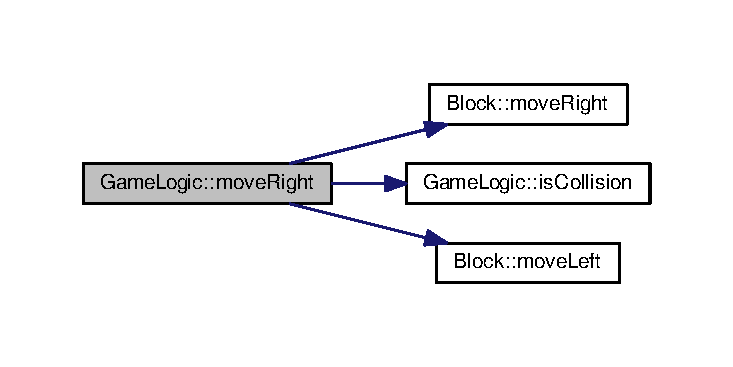
\includegraphics[width=350pt]{class_game_logic_a6213333800f3aa800ea448ad3ee3ea7c_cgraph}
\end{center}
\end{figure}




이 함수를 호출하는 함수들에 대한 그래프입니다.\+:
\nopagebreak
\begin{figure}[H]
\begin{center}
\leavevmode
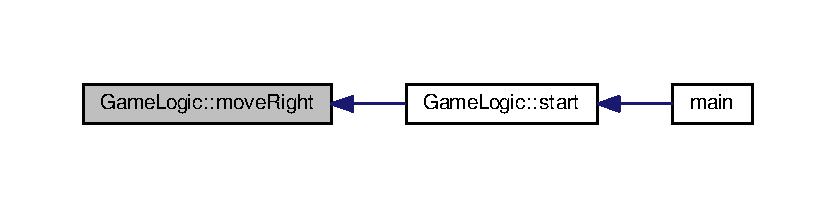
\includegraphics[width=350pt]{class_game_logic_a6213333800f3aa800ea448ad3ee3ea7c_icgraph}
\end{center}
\end{figure}


\index{Game\+Logic@{Game\+Logic}!next\+Level@{next\+Level}}
\index{next\+Level@{next\+Level}!Game\+Logic@{Game\+Logic}}
\subsubsection[{\texorpdfstring{next\+Level()}{nextLevel()}}]{\setlength{\rightskip}{0pt plus 5cm}void Game\+Logic\+::next\+Level (
\begin{DoxyParamCaption}
{}
\end{DoxyParamCaption}
)\hspace{0.3cm}{\ttfamily [private]}}\hypertarget{class_game_logic_a5cc64703af4a64975fe24aa5c1d3c711}{}\label{class_game_logic_a5cc64703af4a64975fe24aa5c1d3c711}


level system 

interval for make difference with level

game clear if interval take negative value 

Game\+Logic.\+cpp 파일의 331 번째 라인에서 정의되었습니다.


\begin{DoxyCode}
331                           \{
332     \hyperlink{myio_8cpp_afce36429cc875312f4476969820ebb51}{printColorString}(30, 3, 0, \textcolor{stringliteral}{"LEVEL"});
333     \textcolor{keywordtype}{char} \hyperlink{class_game_logic_a64ebe1cc14b91b935608ae4455fe3745}{score}[10];
334     sprintf(score, \textcolor{stringliteral}{"%2d"}, \hyperlink{class_game_logic_aca26b3a67b4bb5d5d477f9873826aae8}{level});
335     \hyperlink{myio_8cpp_afce36429cc875312f4476969820ebb51}{printColorString}(30, 4, 0, score);
336     \hyperlink{class_game_logic_ab630a474170a2878d0c5ba8556e3fb39}{clearLines} = 0;
337 
338     \hyperlink{class_game_logic_ab9459c489b9c7bba90895756f373afc6}{interval} -= 5000;
339     \textcolor{keywordflow}{if} (\hyperlink{class_game_logic_ab9459c489b9c7bba90895756f373afc6}{interval} <= 0) \{
340         \hyperlink{class_game_logic_abf26417f7a1fff03e6639b8bd69490f0}{gameClear}();
341     \}
342 \}
\end{DoxyCode}


이 함수 내부에서 호출하는 함수들에 대한 그래프입니다.\+:
\nopagebreak
\begin{figure}[H]
\begin{center}
\leavevmode
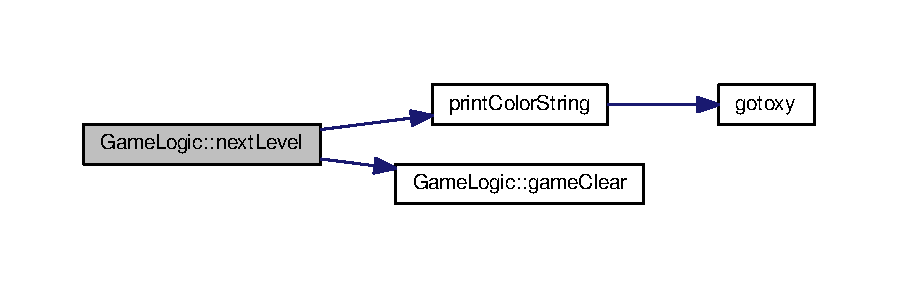
\includegraphics[width=350pt]{class_game_logic_a5cc64703af4a64975fe24aa5c1d3c711_cgraph}
\end{center}
\end{figure}




이 함수를 호출하는 함수들에 대한 그래프입니다.\+:
\nopagebreak
\begin{figure}[H]
\begin{center}
\leavevmode
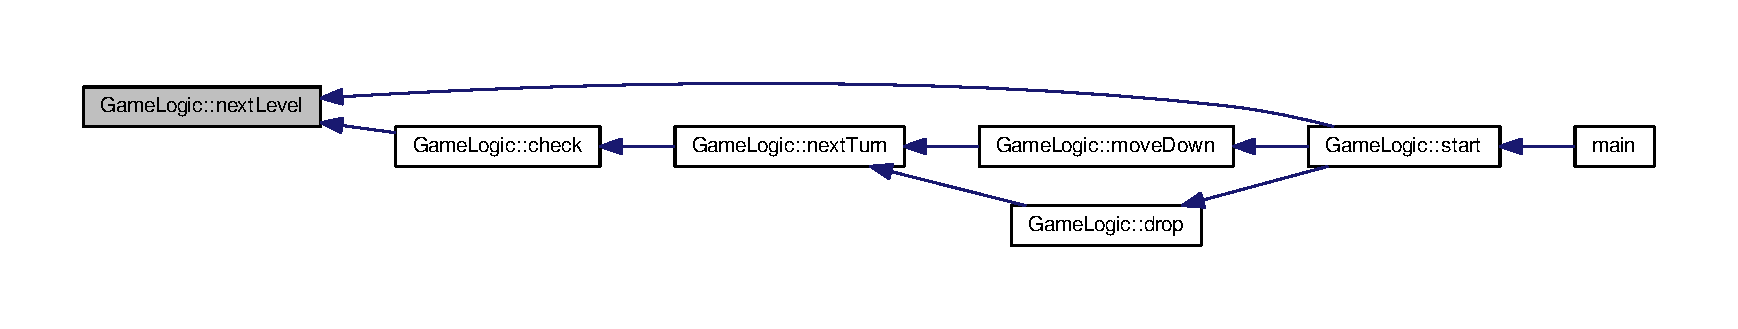
\includegraphics[width=350pt]{class_game_logic_a5cc64703af4a64975fe24aa5c1d3c711_icgraph}
\end{center}
\end{figure}


\index{Game\+Logic@{Game\+Logic}!next\+Turn@{next\+Turn}}
\index{next\+Turn@{next\+Turn}!Game\+Logic@{Game\+Logic}}
\subsubsection[{\texorpdfstring{next\+Turn()}{nextTurn()}}]{\setlength{\rightskip}{0pt plus 5cm}void Game\+Logic\+::next\+Turn (
\begin{DoxyParamCaption}
{}
\end{DoxyParamCaption}
)\hspace{0.3cm}{\ttfamily [private]}}\hypertarget{class_game_logic_a70b7fcd97d321dfb9d2130f864ddac3b}{}\label{class_game_logic_a70b7fcd97d321dfb9d2130f864ddac3b}
보드에 저장

새블럭 생성

Game\+Logic.\+cpp 파일의 201 번째 라인에서 정의되었습니다.


\begin{DoxyCode}
201                          \{
206     \textcolor{keywordflow}{for} (\textcolor{keywordtype}{int} i = 0; i < 4; i++) \{
207         \hyperlink{class_game_logic_a71071a20595279a580d18dfa60ed4a1c}{board}[\hyperlink{class_game_logic_a499d9b05317bb6a77bf3521f42a6638a}{block}.\hyperlink{class_block_aeb5dd312b719966752ba4b38720a4535}{current}.\hyperlink{struct_point_a2e1b5fb2b2a83571f5c0bc0f66a73cf7}{y} + \hyperlink{class_game_logic_a499d9b05317bb6a77bf3521f42a6638a}{block}.\hyperlink{class_block_ae1a4e97236e1e5f04d21fc9227b8c3a8}{shape}[i].\hyperlink{struct_point_a2e1b5fb2b2a83571f5c0bc0f66a73cf7}{y}][
      \hyperlink{class_game_logic_a499d9b05317bb6a77bf3521f42a6638a}{block}.\hyperlink{class_block_aeb5dd312b719966752ba4b38720a4535}{current}.\hyperlink{struct_point_a8c779e11e694b20e0946105a9f5de842}{x} + \hyperlink{class_game_logic_a499d9b05317bb6a77bf3521f42a6638a}{block}.\hyperlink{class_block_ae1a4e97236e1e5f04d21fc9227b8c3a8}{shape}[i].\hyperlink{struct_point_a8c779e11e694b20e0946105a9f5de842}{x}] = \hyperlink{class_game_logic_a499d9b05317bb6a77bf3521f42a6638a}{block}.\hyperlink{class_block_a11fa34418f20b6613d0ceeea8fc71d25}{color};
208     \}
209     \hyperlink{class_game_logic_a499d9b05317bb6a77bf3521f42a6638a}{block}.\hyperlink{class_block_a24e9792df444cc3cd9cd9c28a62f5abd}{refresh}();
210     \hyperlink{class_game_logic_afabf48aab0520a7ecd576bfc178d4767}{check}(\hyperlink{class_game_logic_a499d9b05317bb6a77bf3521f42a6638a}{block});
216     \hyperlink{class_game_logic_a499d9b05317bb6a77bf3521f42a6638a}{block} = \hyperlink{class_game_logic_a42f7be1948bf9cf0a8ff05d7544f62bc}{next};
217     \hyperlink{class_game_logic_a42f7be1948bf9cf0a8ff05d7544f62bc}{next} = \hyperlink{class_block}{Block}();
218     \hyperlink{class_game_logic_a81fa5e44fb6dc431c926f7c3fd0b7cdb}{refreshNextBlock}();
219 
220     \textcolor{keywordflow}{if} (\hyperlink{class_game_logic_a1c534033fe42c8af4fb0e11e3fed2cfa}{isCollision}()) \{
221         \hyperlink{class_game_logic_af6ba400e79f01e5c59f48f55273894e6}{gameOver}();
222     \}
223 \}
\end{DoxyCode}


이 함수 내부에서 호출하는 함수들에 대한 그래프입니다.\+:
\nopagebreak
\begin{figure}[H]
\begin{center}
\leavevmode
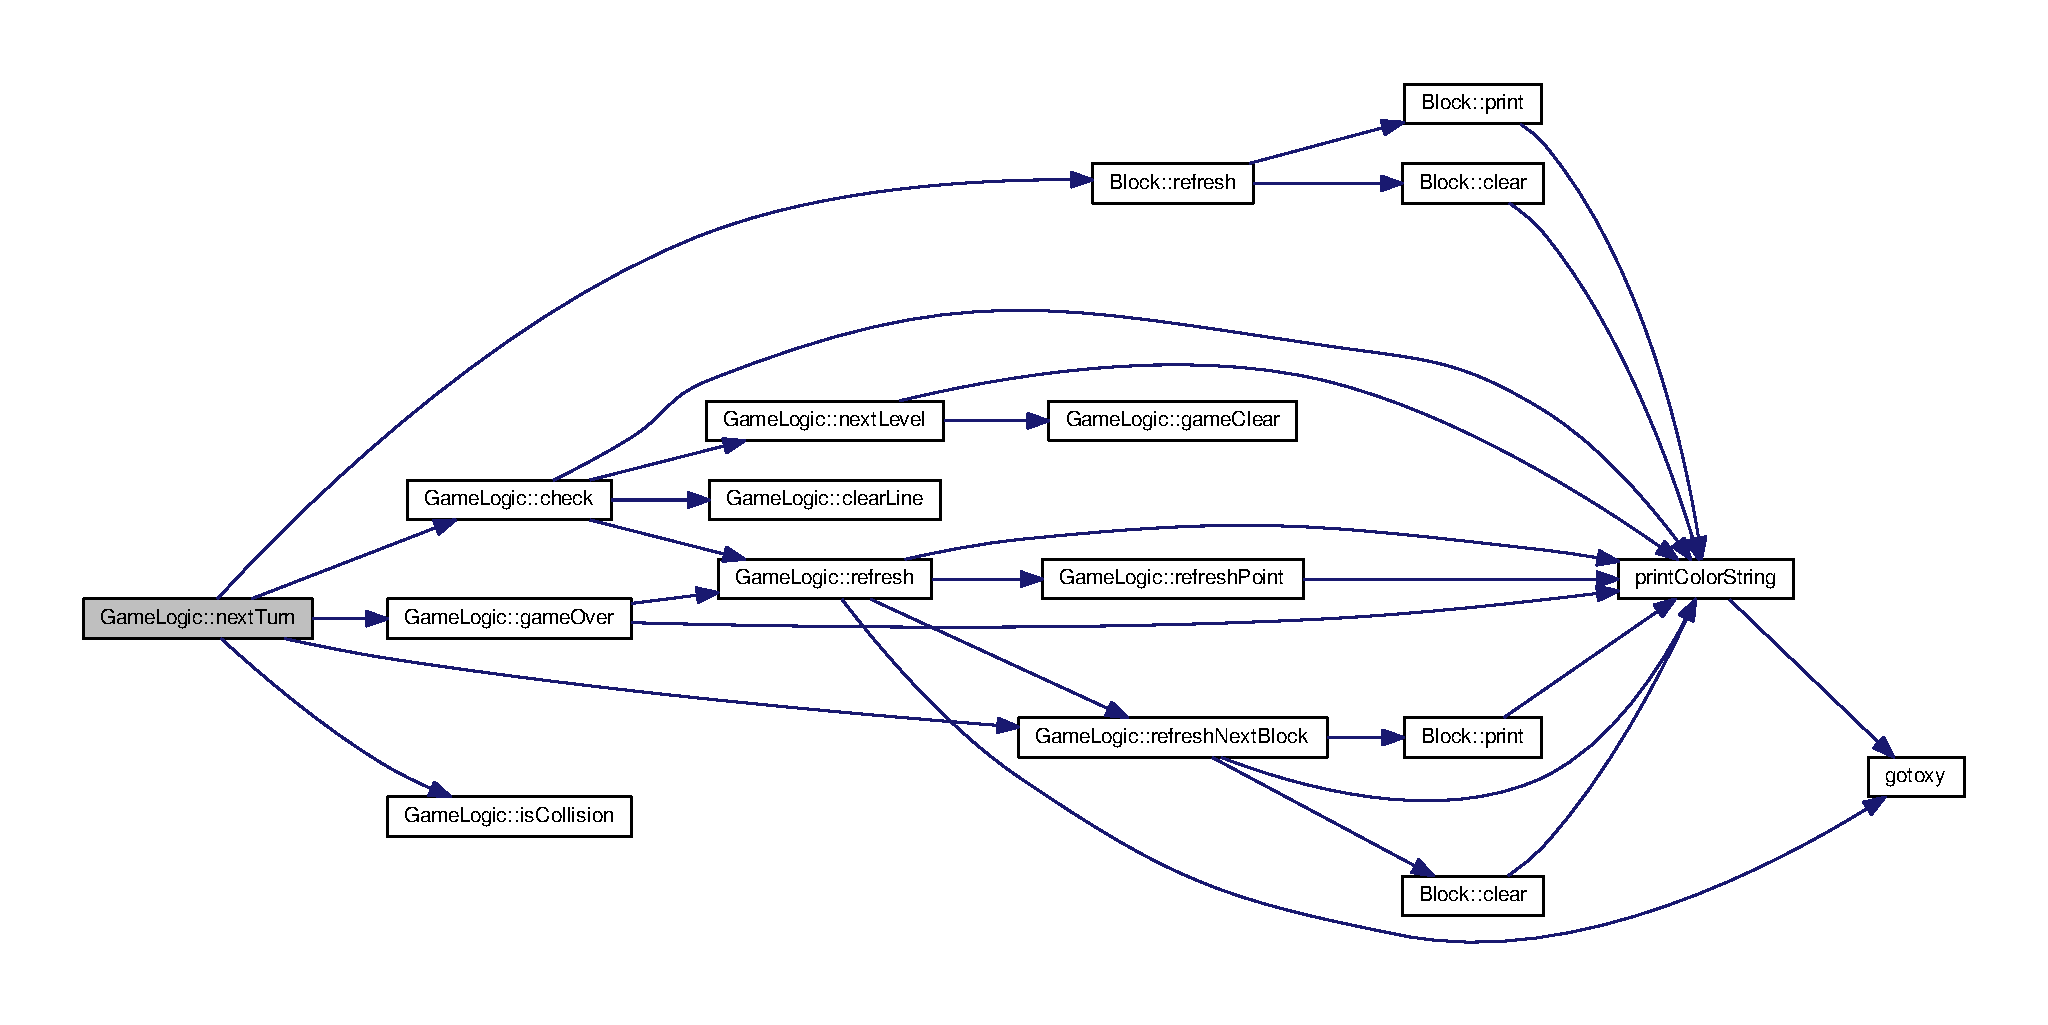
\includegraphics[width=350pt]{class_game_logic_a70b7fcd97d321dfb9d2130f864ddac3b_cgraph}
\end{center}
\end{figure}




이 함수를 호출하는 함수들에 대한 그래프입니다.\+:
\nopagebreak
\begin{figure}[H]
\begin{center}
\leavevmode
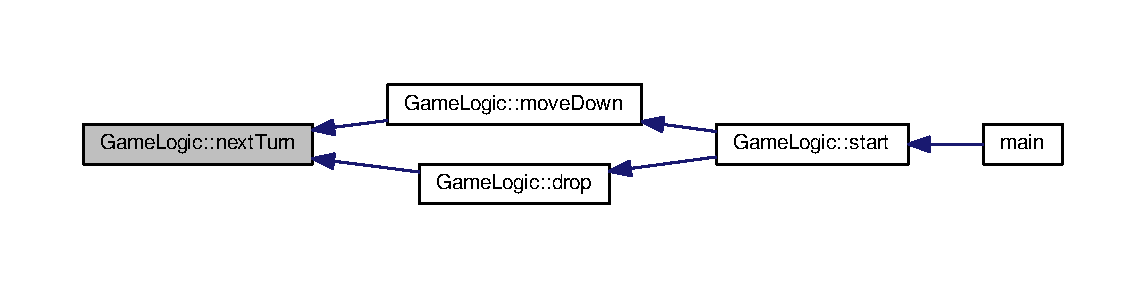
\includegraphics[width=350pt]{class_game_logic_a70b7fcd97d321dfb9d2130f864ddac3b_icgraph}
\end{center}
\end{figure}


\index{Game\+Logic@{Game\+Logic}!print\+Block@{print\+Block}}
\index{print\+Block@{print\+Block}!Game\+Logic@{Game\+Logic}}
\subsubsection[{\texorpdfstring{print\+Block()}{printBlock()}}]{\setlength{\rightskip}{0pt plus 5cm}void Game\+Logic\+::print\+Block (
\begin{DoxyParamCaption}
{}
\end{DoxyParamCaption}
)}\hypertarget{class_game_logic_ad0f9f0e6c978a3b3fa1ff7a2a3d92563}{}\label{class_game_logic_ad0f9f0e6c978a3b3fa1ff7a2a3d92563}


Game\+Logic.\+cpp 파일의 103 번째 라인에서 정의되었습니다.


\begin{DoxyCode}
103                            \{
104     \hyperlink{class_game_logic_a499d9b05317bb6a77bf3521f42a6638a}{block}.\hyperlink{class_block_a24e9792df444cc3cd9cd9c28a62f5abd}{refresh}();
105 \}
\end{DoxyCode}


이 함수 내부에서 호출하는 함수들에 대한 그래프입니다.\+:
\nopagebreak
\begin{figure}[H]
\begin{center}
\leavevmode
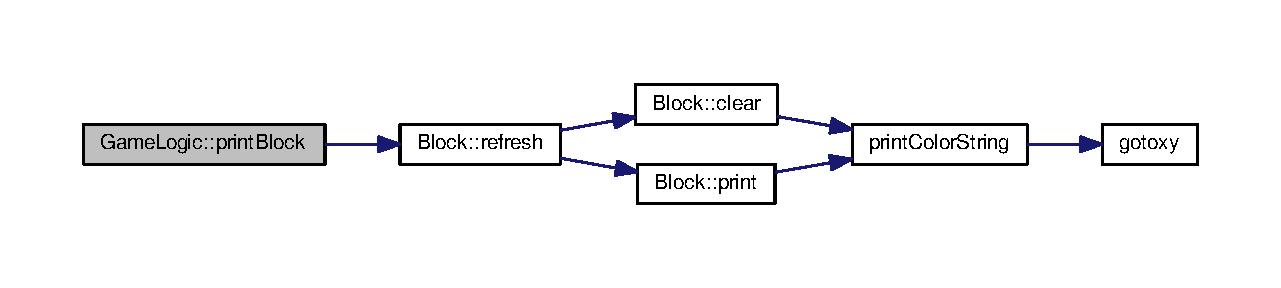
\includegraphics[width=350pt]{class_game_logic_ad0f9f0e6c978a3b3fa1ff7a2a3d92563_cgraph}
\end{center}
\end{figure}




이 함수를 호출하는 함수들에 대한 그래프입니다.\+:
\nopagebreak
\begin{figure}[H]
\begin{center}
\leavevmode
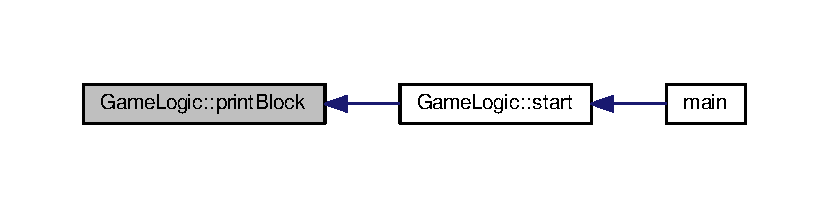
\includegraphics[width=350pt]{class_game_logic_ad0f9f0e6c978a3b3fa1ff7a2a3d92563_icgraph}
\end{center}
\end{figure}


\index{Game\+Logic@{Game\+Logic}!refresh@{refresh}}
\index{refresh@{refresh}!Game\+Logic@{Game\+Logic}}
\subsubsection[{\texorpdfstring{refresh()}{refresh()}}]{\setlength{\rightskip}{0pt plus 5cm}void Game\+Logic\+::refresh (
\begin{DoxyParamCaption}
{}
\end{DoxyParamCaption}
)\hspace{0.3cm}{\ttfamily [private]}}\hypertarget{class_game_logic_aff831622dc54c1737e76b00d0d44ccef}{}\label{class_game_logic_aff831622dc54c1737e76b00d0d44ccef}


Game\+Logic.\+cpp 파일의 284 번째 라인에서 정의되었습니다.


\begin{DoxyCode}
284                         \{
285 
286     \textcolor{keywordflow}{for} (\textcolor{keywordtype}{int} i = 0; i < \hyperlink{_game_logic_8h_af728b7647e0b8c49832983a31f9a2e9b}{HEIGHT}; i++) \{
287         \hyperlink{myio_8cpp_ae824443b3f661414ba1f2718e17fe97d}{gotoxy}(\hyperlink{class_block_ad456f4794a480711f7057e1f270d93c2}{Block::zero}.x - 2, \hyperlink{class_block_ad456f4794a480711f7057e1f270d93c2}{Block::zero}.y + i);
288         putchar(\textcolor{charliteral}{'*'});
289 
290         \textcolor{keywordflow}{for} (\textcolor{keywordtype}{int} x = 0; x < \hyperlink{_game_logic_8h_a9649ab8139c4c2ea5c93625b30d92a05}{WIDTH}; x++) \{
291             \textcolor{keywordflow}{if} (\hyperlink{class_game_logic_a71071a20595279a580d18dfa60ed4a1c}{board}[i][x]) \{
292                 \hyperlink{myio_8cpp_afce36429cc875312f4476969820ebb51}{printColorString}(x * 2 + \hyperlink{class_block_ad456f4794a480711f7057e1f270d93c2}{Block::zero}.x, 
      \hyperlink{class_block_ad456f4794a480711f7057e1f270d93c2}{Block::zero}.y + i, \hyperlink{class_game_logic_a71071a20595279a580d18dfa60ed4a1c}{board}[i][x], \hyperlink{class_block_a4cb64c2c20884eed68c24c6147f68514}{Block::BLOCK});
293             \} \textcolor{keywordflow}{else} \{
294                 \hyperlink{myio_8cpp_afce36429cc875312f4476969820ebb51}{printColorString}(x * 2 + \hyperlink{class_block_ad456f4794a480711f7057e1f270d93c2}{Block::zero}.x, 
      \hyperlink{class_block_ad456f4794a480711f7057e1f270d93c2}{Block::zero}.y + i, \hyperlink{class_game_logic_a71071a20595279a580d18dfa60ed4a1c}{board}[i][x], \hyperlink{class_block_a11bcda9589b54be35a8905ca7be7310e}{Block::CLEAR});
295             \}
296         \}
297         \hyperlink{myio_8cpp_ae824443b3f661414ba1f2718e17fe97d}{gotoxy}(\hyperlink{class_block_ad456f4794a480711f7057e1f270d93c2}{Block::zero}.x + WIDTH * 2, \hyperlink{class_block_ad456f4794a480711f7057e1f270d93c2}{Block::zero}.y + i);
298         putchar(\textcolor{charliteral}{'*'});
299     \}
300     \hyperlink{myio_8cpp_ae824443b3f661414ba1f2718e17fe97d}{gotoxy}(\hyperlink{class_block_ad456f4794a480711f7057e1f270d93c2}{Block::zero}.x - 2, \hyperlink{class_block_ad456f4794a480711f7057e1f270d93c2}{Block::zero}.y + HEIGHT);
301     printf(\textcolor{stringliteral}{"***********************"});
302     \hyperlink{class_game_logic_a81fa5e44fb6dc431c926f7c3fd0b7cdb}{refreshNextBlock}();
303     \hyperlink{class_game_logic_a3f19ca1ad6a1c829afe571f7ac25d3c5}{refreshPoint}();
304 
305 \}
\end{DoxyCode}


이 함수 내부에서 호출하는 함수들에 대한 그래프입니다.\+:
\nopagebreak
\begin{figure}[H]
\begin{center}
\leavevmode
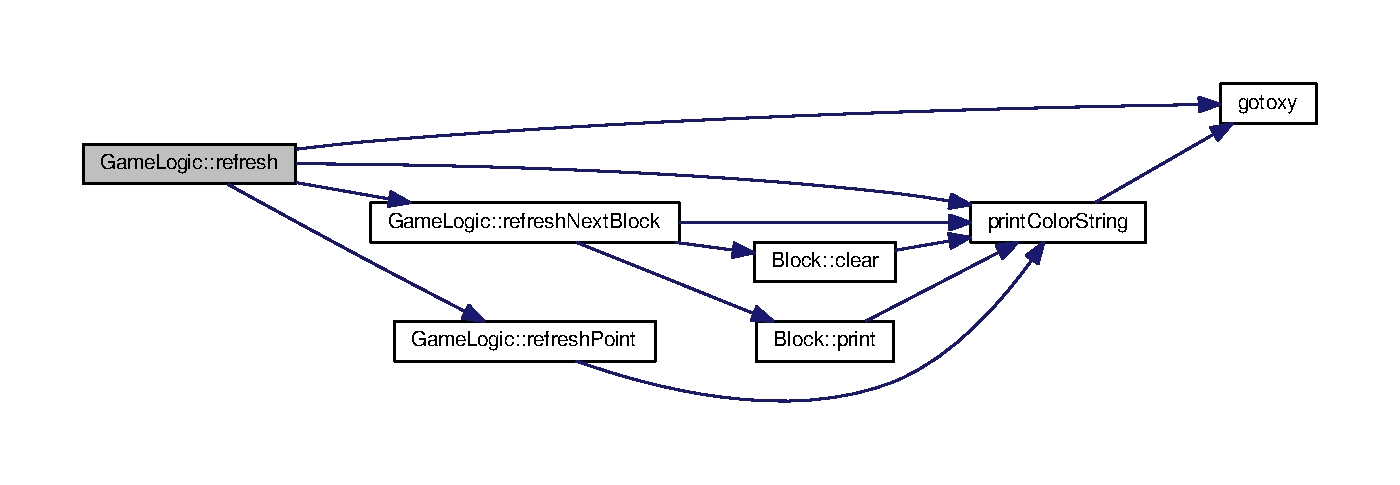
\includegraphics[width=350pt]{class_game_logic_aff831622dc54c1737e76b00d0d44ccef_cgraph}
\end{center}
\end{figure}




이 함수를 호출하는 함수들에 대한 그래프입니다.\+:
\nopagebreak
\begin{figure}[H]
\begin{center}
\leavevmode
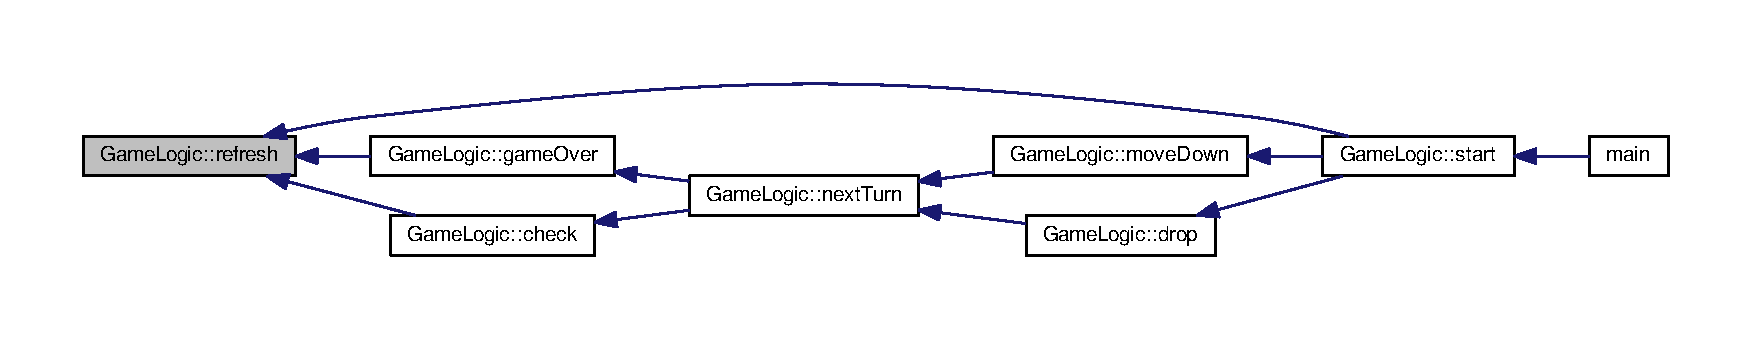
\includegraphics[width=350pt]{class_game_logic_aff831622dc54c1737e76b00d0d44ccef_icgraph}
\end{center}
\end{figure}


\index{Game\+Logic@{Game\+Logic}!refresh\+Next\+Block@{refresh\+Next\+Block}}
\index{refresh\+Next\+Block@{refresh\+Next\+Block}!Game\+Logic@{Game\+Logic}}
\subsubsection[{\texorpdfstring{refresh\+Next\+Block()}{refreshNextBlock()}}]{\setlength{\rightskip}{0pt plus 5cm}void Game\+Logic\+::refresh\+Next\+Block (
\begin{DoxyParamCaption}
{}
\end{DoxyParamCaption}
)\hspace{0.3cm}{\ttfamily [private]}}\hypertarget{class_game_logic_a81fa5e44fb6dc431c926f7c3fd0b7cdb}{}\label{class_game_logic_a81fa5e44fb6dc431c926f7c3fd0b7cdb}


Game\+Logic.\+cpp 파일의 307 번째 라인에서 정의되었습니다.


\begin{DoxyCode}
307                                  \{
308     \hyperlink{myio_8cpp_afce36429cc875312f4476969820ebb51}{printColorString}(30, 7, 0, \textcolor{stringliteral}{"┌────────┐"});
309     \textcolor{keywordflow}{for} (\textcolor{keywordtype}{int} i = 0; i < 4; i++) \{
310         \hyperlink{myio_8cpp_afce36429cc875312f4476969820ebb51}{printColorString}(30, 8 + i, 0, \textcolor{stringliteral}{"│        │"});
311     \}
312     \hyperlink{myio_8cpp_afce36429cc875312f4476969820ebb51}{printColorString}(30, 12, 0, \textcolor{stringliteral}{"└────────┘"});
313     \hyperlink{class_game_logic_a42f7be1948bf9cf0a8ff05d7544f62bc}{next}.\hyperlink{class_block_a5ea55096829ff27961b989409283cd86}{clear}(31, 8);
314     \hyperlink{class_game_logic_a42f7be1948bf9cf0a8ff05d7544f62bc}{next}.\hyperlink{class_block_a6735096bf1a9678a688b98782bd1b226}{print}(31, 8);
315 \}
\end{DoxyCode}


이 함수 내부에서 호출하는 함수들에 대한 그래프입니다.\+:
\nopagebreak
\begin{figure}[H]
\begin{center}
\leavevmode
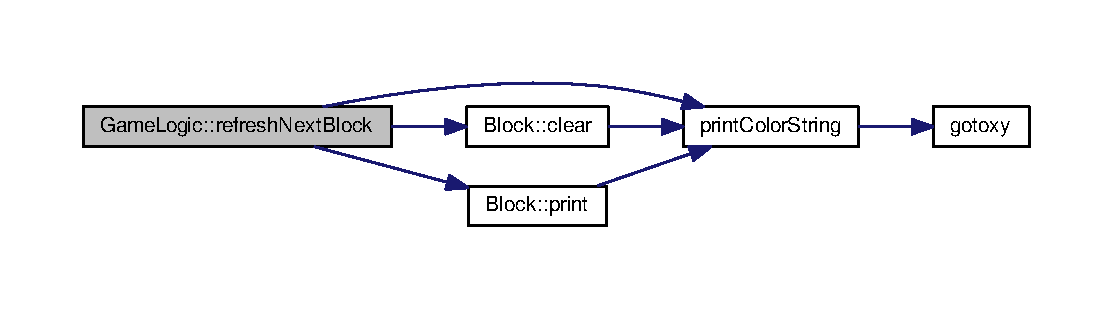
\includegraphics[width=350pt]{class_game_logic_a81fa5e44fb6dc431c926f7c3fd0b7cdb_cgraph}
\end{center}
\end{figure}




이 함수를 호출하는 함수들에 대한 그래프입니다.\+:
\nopagebreak
\begin{figure}[H]
\begin{center}
\leavevmode
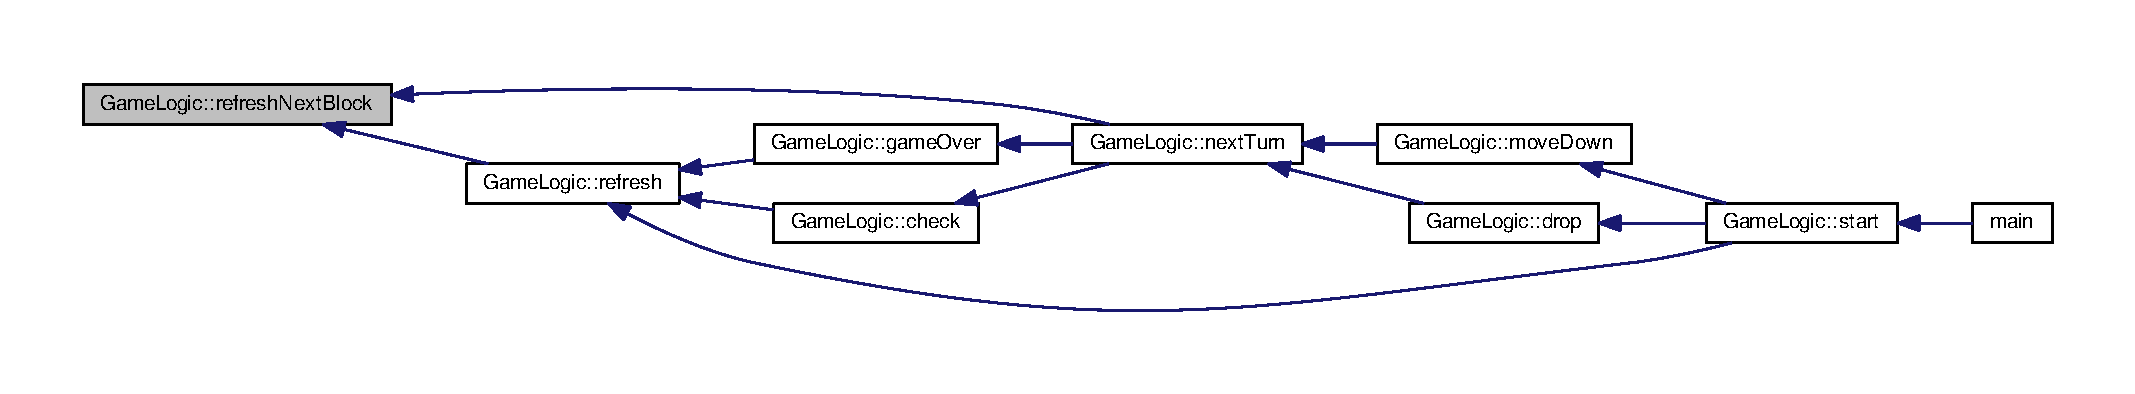
\includegraphics[width=350pt]{class_game_logic_a81fa5e44fb6dc431c926f7c3fd0b7cdb_icgraph}
\end{center}
\end{figure}


\index{Game\+Logic@{Game\+Logic}!refresh\+Point@{refresh\+Point}}
\index{refresh\+Point@{refresh\+Point}!Game\+Logic@{Game\+Logic}}
\subsubsection[{\texorpdfstring{refresh\+Point()}{refreshPoint()}}]{\setlength{\rightskip}{0pt plus 5cm}void Game\+Logic\+::refresh\+Point (
\begin{DoxyParamCaption}
{}
\end{DoxyParamCaption}
)\hspace{0.3cm}{\ttfamily [private]}}\hypertarget{class_game_logic_a3f19ca1ad6a1c829afe571f7ac25d3c5}{}\label{class_game_logic_a3f19ca1ad6a1c829afe571f7ac25d3c5}


Game\+Logic.\+cpp 파일의 317 번째 라인에서 정의되었습니다.


\begin{DoxyCode}
317                              \{
318     \hyperlink{myio_8cpp_afce36429cc875312f4476969820ebb51}{printColorString}(30, 5, 0, \textcolor{stringliteral}{"SCORE"});
319     \textcolor{keywordtype}{char} \hyperlink{class_game_logic_a64ebe1cc14b91b935608ae4455fe3745}{score}[10];
320     sprintf(score, \textcolor{stringliteral}{"%08d"}, this->score);
321     \hyperlink{myio_8cpp_afce36429cc875312f4476969820ebb51}{printColorString}(30, 6, 0, score);
322 \}
\end{DoxyCode}


이 함수 내부에서 호출하는 함수들에 대한 그래프입니다.\+:
\nopagebreak
\begin{figure}[H]
\begin{center}
\leavevmode
\includegraphics[width=350pt]{class_game_logic_a3f19ca1ad6a1c829afe571f7ac25d3c5_cgraph}
\end{center}
\end{figure}




이 함수를 호출하는 함수들에 대한 그래프입니다.\+:
\nopagebreak
\begin{figure}[H]
\begin{center}
\leavevmode
\includegraphics[width=350pt]{class_game_logic_a3f19ca1ad6a1c829afe571f7ac25d3c5_icgraph}
\end{center}
\end{figure}


\index{Game\+Logic@{Game\+Logic}!start@{start}}
\index{start@{start}!Game\+Logic@{Game\+Logic}}
\subsubsection[{\texorpdfstring{start()}{start()}}]{\setlength{\rightskip}{0pt plus 5cm}void Game\+Logic\+::start (
\begin{DoxyParamCaption}
{}
\end{DoxyParamCaption}
)}\hypertarget{class_game_logic_aeb7d3db8014da87a18ac744d9f77131d}{}\label{class_game_logic_aeb7d3db8014da87a18ac744d9f77131d}


Game\+Logic.\+cpp 파일의 47 번째 라인에서 정의되었습니다.


\begin{DoxyCode}
47                       \{
48     \hyperlink{class_game_logic_ae09fc4252ad9db62b810117567783880}{isNotGameOver}=\textcolor{keyword}{true};
49     \hyperlink{class_game_logic_a499d9b05317bb6a77bf3521f42a6638a}{block} = \hyperlink{class_block}{Block}();
50     \hyperlink{class_game_logic_a42f7be1948bf9cf0a8ff05d7544f62bc}{next} = \hyperlink{class_block}{Block}();
51     \hyperlink{class_game_logic_a64ebe1cc14b91b935608ae4455fe3745}{score} = 0;
52     \hyperlink{class_game_logic_ab9459c489b9c7bba90895756f373afc6}{interval} = 105000;
53     \hyperlink{class_game_logic_ab630a474170a2878d0c5ba8556e3fb39}{clearLines} = 0;
54     \hyperlink{class_game_logic_aca26b3a67b4bb5d5d477f9873826aae8}{level} = 1;
55     \hyperlink{class_game_logic_a5cc64703af4a64975fe24aa5c1d3c711}{nextLevel}();
56     \hyperlink{class_game_logic_aff831622dc54c1737e76b00d0d44ccef}{refresh}();
57     \textcolor{keywordtype}{int} n;
58     \textcolor{keywordtype}{unsigned} \textcolor{keywordtype}{char} key;
59     clock\_t refresh1 = clock();
60     clock\_t current = refresh1;
61     clock\_t blockDown = refresh1;
62     \textcolor{keywordflow}{while} (\hyperlink{class_game_logic_ae09fc4252ad9db62b810117567783880}{isNotGameOver}) \{
63         current = clock();
64         \textcolor{keywordflow}{if} (current - refresh1 > 16000) \{
65             refresh1 = current;
66             \hyperlink{class_game_logic_ad0f9f0e6c978a3b3fa1ff7a2a3d92563}{printBlock}();
67         \}
68         \textcolor{keywordflow}{if} (current - blockDown > \hyperlink{class_game_logic_ab9459c489b9c7bba90895756f373afc6}{interval}) \{
69             \hyperlink{class_game_logic_a36b04a5ca335351249db8cc77019c216}{moveDown}();
70             blockDown = current;
71         \}
72         n = getchar();
73         \textcolor{keywordflow}{if} (n != EOF) \{
74             key = n;
75             \textcolor{keywordflow}{switch} (key) \{
76             \textcolor{keywordflow}{case} \textcolor{charliteral}{'Q'}:
77                 \hyperlink{class_game_logic_ae09fc4252ad9db62b810117567783880}{isNotGameOver}=\textcolor{keyword}{false};
78                 this->\hyperlink{class_game_logic_a6a95fb9e16b411f1149dcdb463cdc3a5}{isRun} = \textcolor{keyword}{false};
79                 \textcolor{keywordflow}{break};
80             \textcolor{keywordflow}{case} \hyperlink{_game_logic_8cpp_a1965eaca47dbf3f87acdafc2208f04eb}{UP}:
81                 \hyperlink{class_game_logic_abd2dece64def6dc89e0b116fdca83483}{transforse}();
82                 \textcolor{keywordflow}{break};
83             \textcolor{keywordflow}{case} \hyperlink{_game_logic_8cpp_a4193cd1c8c2e6ebd0e056fa2364a663f}{DOWN}:
84                 \hyperlink{class_game_logic_a36b04a5ca335351249db8cc77019c216}{moveDown}();
85                 \textcolor{keywordflow}{break};
86             \textcolor{keywordflow}{case} \hyperlink{_game_logic_8cpp_a80fb826a684cf3f0d306b22aa100ddac}{RIGHT}:
87                 \hyperlink{class_game_logic_a6213333800f3aa800ea448ad3ee3ea7c}{moveRight}();
88                 \textcolor{keywordflow}{break};
89             \textcolor{keywordflow}{case} \hyperlink{_game_logic_8cpp_a437ef08681e7210d6678427030446a54}{LEFT}:
90                 \hyperlink{class_game_logic_a0e6c1ee03971cf619212f8bb4d5fbc83}{moveLeft}();
91                 \textcolor{keywordflow}{break};
92             \textcolor{keywordflow}{case} \textcolor{charliteral}{' '}:
93                 \hyperlink{class_game_logic_a90faee03fd4311eab796ae7dc582078d}{drop}();
94                 \textcolor{keywordflow}{break};
95             \textcolor{keywordflow}{default}:
96                 \textcolor{keywordflow}{break};
97             \}
98         \}
99         \hyperlink{myio_8cpp_ae824443b3f661414ba1f2718e17fe97d}{gotoxy}(80, 24);
100     \}
101 \}
\end{DoxyCode}


이 함수 내부에서 호출하는 함수들에 대한 그래프입니다.\+:
\nopagebreak
\begin{figure}[H]
\begin{center}
\leavevmode
\includegraphics[width=350pt]{class_game_logic_aeb7d3db8014da87a18ac744d9f77131d_cgraph}
\end{center}
\end{figure}




이 함수를 호출하는 함수들에 대한 그래프입니다.\+:
\nopagebreak
\begin{figure}[H]
\begin{center}
\leavevmode
\includegraphics[width=246pt]{class_game_logic_aeb7d3db8014da87a18ac744d9f77131d_icgraph}
\end{center}
\end{figure}


\index{Game\+Logic@{Game\+Logic}!transforse@{transforse}}
\index{transforse@{transforse}!Game\+Logic@{Game\+Logic}}
\subsubsection[{\texorpdfstring{transforse()}{transforse()}}]{\setlength{\rightskip}{0pt plus 5cm}void Game\+Logic\+::transforse (
\begin{DoxyParamCaption}
{}
\end{DoxyParamCaption}
)}\hypertarget{class_game_logic_abd2dece64def6dc89e0b116fdca83483}{}\label{class_game_logic_abd2dece64def6dc89e0b116fdca83483}


Game\+Logic.\+cpp 파일의 136 번째 라인에서 정의되었습니다.


\begin{DoxyCode}
136                            \{
137     \hyperlink{class_block}{Block} temp = \hyperlink{class_game_logic_a499d9b05317bb6a77bf3521f42a6638a}{block};
138     \hyperlink{class_game_logic_a499d9b05317bb6a77bf3521f42a6638a}{block}.\hyperlink{class_block_a9cc446ec51a125982c41e67af63059b0}{transpose}();
139     \textcolor{keywordflow}{if} (\hyperlink{class_game_logic_a1c534033fe42c8af4fb0e11e3fed2cfa}{isCollision}()) \{
140         \hyperlink{class_game_logic_a499d9b05317bb6a77bf3521f42a6638a}{block}.\hyperlink{class_block_a18bfe78145650d1b13267000feea278b}{reversTranspose}();
141     \} \textcolor{keywordflow}{else} \{
142         temp.\hyperlink{class_block_a5ea55096829ff27961b989409283cd86}{clear}();
143         \hyperlink{class_game_logic_a499d9b05317bb6a77bf3521f42a6638a}{block}.\hyperlink{class_block_a6735096bf1a9678a688b98782bd1b226}{print}();
144     \}
145 \}
\end{DoxyCode}


이 함수 내부에서 호출하는 함수들에 대한 그래프입니다.\+:
\nopagebreak
\begin{figure}[H]
\begin{center}
\leavevmode
\includegraphics[width=350pt]{class_game_logic_abd2dece64def6dc89e0b116fdca83483_cgraph}
\end{center}
\end{figure}




이 함수를 호출하는 함수들에 대한 그래프입니다.\+:
\nopagebreak
\begin{figure}[H]
\begin{center}
\leavevmode
\includegraphics[width=350pt]{class_game_logic_abd2dece64def6dc89e0b116fdca83483_icgraph}
\end{center}
\end{figure}




\subsection{멤버 데이타 문서화}
\index{Game\+Logic@{Game\+Logic}!block@{block}}
\index{block@{block}!Game\+Logic@{Game\+Logic}}
\subsubsection[{\texorpdfstring{block}{block}}]{\setlength{\rightskip}{0pt plus 5cm}{\bf Block} Game\+Logic\+::block\hspace{0.3cm}{\ttfamily [private]}}\hypertarget{class_game_logic_a499d9b05317bb6a77bf3521f42a6638a}{}\label{class_game_logic_a499d9b05317bb6a77bf3521f42a6638a}


Game\+Logic.\+h 파일의 41 번째 라인에서 정의되었습니다.

\index{Game\+Logic@{Game\+Logic}!board@{board}}
\index{board@{board}!Game\+Logic@{Game\+Logic}}
\subsubsection[{\texorpdfstring{board}{board}}]{\setlength{\rightskip}{0pt plus 5cm}char$\ast$ Game\+Logic\+::board\mbox{[}{\bf H\+E\+I\+G\+HT}\mbox{]}}\hypertarget{class_game_logic_a71071a20595279a580d18dfa60ed4a1c}{}\label{class_game_logic_a71071a20595279a580d18dfa60ed4a1c}


Game\+Logic.\+h 파일의 22 번째 라인에서 정의되었습니다.

\index{Game\+Logic@{Game\+Logic}!clear\+Lines@{clear\+Lines}}
\index{clear\+Lines@{clear\+Lines}!Game\+Logic@{Game\+Logic}}
\subsubsection[{\texorpdfstring{clear\+Lines}{clearLines}}]{\setlength{\rightskip}{0pt plus 5cm}int Game\+Logic\+::clear\+Lines}\hypertarget{class_game_logic_ab630a474170a2878d0c5ba8556e3fb39}{}\label{class_game_logic_ab630a474170a2878d0c5ba8556e3fb39}


Game\+Logic.\+h 파일의 20 번째 라인에서 정의되었습니다.

\index{Game\+Logic@{Game\+Logic}!interval@{interval}}
\index{interval@{interval}!Game\+Logic@{Game\+Logic}}
\subsubsection[{\texorpdfstring{interval}{interval}}]{\setlength{\rightskip}{0pt plus 5cm}int Game\+Logic\+::interval}\hypertarget{class_game_logic_ab9459c489b9c7bba90895756f373afc6}{}\label{class_game_logic_ab9459c489b9c7bba90895756f373afc6}


Game\+Logic.\+h 파일의 19 번째 라인에서 정의되었습니다.

\index{Game\+Logic@{Game\+Logic}!is\+Not\+Game\+Over@{is\+Not\+Game\+Over}}
\index{is\+Not\+Game\+Over@{is\+Not\+Game\+Over}!Game\+Logic@{Game\+Logic}}
\subsubsection[{\texorpdfstring{is\+Not\+Game\+Over}{isNotGameOver}}]{\setlength{\rightskip}{0pt plus 5cm}bool Game\+Logic\+::is\+Not\+Game\+Over\hspace{0.3cm}{\ttfamily [private]}}\hypertarget{class_game_logic_ae09fc4252ad9db62b810117567783880}{}\label{class_game_logic_ae09fc4252ad9db62b810117567783880}


Game\+Logic.\+h 파일의 43 번째 라인에서 정의되었습니다.

\index{Game\+Logic@{Game\+Logic}!is\+Run@{is\+Run}}
\index{is\+Run@{is\+Run}!Game\+Logic@{Game\+Logic}}
\subsubsection[{\texorpdfstring{is\+Run}{isRun}}]{\setlength{\rightskip}{0pt plus 5cm}bool Game\+Logic\+::is\+Run}\hypertarget{class_game_logic_a6a95fb9e16b411f1149dcdb463cdc3a5}{}\label{class_game_logic_a6a95fb9e16b411f1149dcdb463cdc3a5}


Game\+Logic.\+h 파일의 18 번째 라인에서 정의되었습니다.

\index{Game\+Logic@{Game\+Logic}!level@{level}}
\index{level@{level}!Game\+Logic@{Game\+Logic}}
\subsubsection[{\texorpdfstring{level}{level}}]{\setlength{\rightskip}{0pt plus 5cm}int Game\+Logic\+::level\hspace{0.3cm}{\ttfamily [private]}}\hypertarget{class_game_logic_aca26b3a67b4bb5d5d477f9873826aae8}{}\label{class_game_logic_aca26b3a67b4bb5d5d477f9873826aae8}


Game\+Logic.\+h 파일의 55 번째 라인에서 정의되었습니다.

\index{Game\+Logic@{Game\+Logic}!next@{next}}
\index{next@{next}!Game\+Logic@{Game\+Logic}}
\subsubsection[{\texorpdfstring{next}{next}}]{\setlength{\rightskip}{0pt plus 5cm}{\bf Block} Game\+Logic\+::next\hspace{0.3cm}{\ttfamily [private]}}\hypertarget{class_game_logic_a42f7be1948bf9cf0a8ff05d7544f62bc}{}\label{class_game_logic_a42f7be1948bf9cf0a8ff05d7544f62bc}


Game\+Logic.\+h 파일의 42 번째 라인에서 정의되었습니다.

\index{Game\+Logic@{Game\+Logic}!score@{score}}
\index{score@{score}!Game\+Logic@{Game\+Logic}}
\subsubsection[{\texorpdfstring{score}{score}}]{\setlength{\rightskip}{0pt plus 5cm}int Game\+Logic\+::score}\hypertarget{class_game_logic_a64ebe1cc14b91b935608ae4455fe3745}{}\label{class_game_logic_a64ebe1cc14b91b935608ae4455fe3745}


Game\+Logic.\+h 파일의 17 번째 라인에서 정의되었습니다.



이 클래스에 대한 문서화 페이지는 다음의 파일들로부터 생성되었습니다.\+:\begin{DoxyCompactItemize}
\item 
\hyperlink{_game_logic_8h}{Game\+Logic.\+h}\item 
\hyperlink{_game_logic_8cpp}{Game\+Logic.\+cpp}\end{DoxyCompactItemize}

\hypertarget{struct_point}{}\section{Point 구조체 참조}
\label{struct_point}\index{Point@{Point}}


{\ttfamily \#include $<$Block.\+h$>$}



Point에 대한 협력 다이어그램\+:
\nopagebreak
\begin{figure}[H]
\begin{center}
\leavevmode
\includegraphics[width=119pt]{struct_point__coll__graph}
\end{center}
\end{figure}
\subsection*{Public 속성}
\begin{DoxyCompactItemize}
\item 
int \hyperlink{struct_point_a8c779e11e694b20e0946105a9f5de842}{x}
\item 
int \hyperlink{struct_point_a2e1b5fb2b2a83571f5c0bc0f66a73cf7}{y}
\end{DoxyCompactItemize}


\subsection{상세한 설명}


Block.\+h 파일의 10 번째 라인에서 정의되었습니다.



\subsection{멤버 데이타 문서화}
\index{Point@{Point}!x@{x}}
\index{x@{x}!Point@{Point}}
\subsubsection[{\texorpdfstring{x}{x}}]{\setlength{\rightskip}{0pt plus 5cm}int Point\+::x}\hypertarget{struct_point_a8c779e11e694b20e0946105a9f5de842}{}\label{struct_point_a8c779e11e694b20e0946105a9f5de842}


Block.\+h 파일의 11 번째 라인에서 정의되었습니다.

\index{Point@{Point}!y@{y}}
\index{y@{y}!Point@{Point}}
\subsubsection[{\texorpdfstring{y}{y}}]{\setlength{\rightskip}{0pt plus 5cm}int Point\+::y}\hypertarget{struct_point_a2e1b5fb2b2a83571f5c0bc0f66a73cf7}{}\label{struct_point_a2e1b5fb2b2a83571f5c0bc0f66a73cf7}


Block.\+h 파일의 11 번째 라인에서 정의되었습니다.



이 구조체에 대한 문서화 페이지는 다음의 파일로부터 생성되었습니다.\+:\begin{DoxyCompactItemize}
\item 
\hyperlink{_block_8h}{Block.\+h}\end{DoxyCompactItemize}

\chapter{파일 문서화}
\hypertarget{_block_8cpp}{}\section{Block.\+cpp 파일 참조}
\label{_block_8cpp}\index{Block.\+cpp@{Block.\+cpp}}


tetis block system  


{\ttfamily \#include \char`\"{}Block.\+h\char`\"{}}\\*
{\ttfamily \#include \char`\"{}myio.\+h\char`\"{}}\\*
{\ttfamily \#include \char`\"{}Game\+Logic.\+h\char`\"{}}\\*
{\ttfamily \#include $<$stdlib.\+h$>$}\\*
{\ttfamily \#include $<$time.\+h$>$}\\*
Block.\+cpp에 대한 include 의존 그래프
\nopagebreak
\begin{figure}[H]
\begin{center}
\leavevmode
\includegraphics[width=350pt]{_block_8cpp__incl}
\end{center}
\end{figure}
\subsection*{매크로}
\begin{DoxyCompactItemize}
\item 
\#define \hyperlink{_block_8cpp_a51591cf51bdd6c1f6015532422e7770e}{Z}~\hyperlink{myio_8h_ad86358bf19927183dd7b4ae215a29731}{C\+O\+L\+O\+R\+\_\+\+R\+ED}
\begin{DoxyCompactList}\small\item\em macro for color of block \end{DoxyCompactList}\item 
\#define \hyperlink{_block_8cpp_af933676109efed7ab34cea71d748a517}{S}~\hyperlink{myio_8h_afc9149f5de51bd9ac4f5ebbfa153f018}{C\+O\+L\+O\+R\+\_\+\+G\+R\+E\+EN}
\item 
\#define \hyperlink{_block_8cpp_a396fecfabe3105afc15a61c209f910f0}{O}~\hyperlink{myio_8h_a928e144dbbe4316dbb854245c7e38de7}{C\+O\+L\+O\+R\+\_\+\+B\+R\+O\+WN}
\item 
\#define \hyperlink{_block_8cpp_ad59246fadffe0205c1ecfcd147c407f6}{J}~\hyperlink{myio_8h_a23c70d699a5a775bc2e1ebeb8603f630}{C\+O\+L\+O\+R\+\_\+\+B\+L\+UE}
\item 
\#define \hyperlink{_block_8cpp_a0acb682b8260ab1c60b918599864e2e5}{T}~\hyperlink{myio_8h_a8deb0beccea721b35bdb1b4f7264fe75}{C\+O\+L\+O\+R\+\_\+\+M\+A\+G\+E\+N\+TA}
\item 
\#define \hyperlink{_block_8cpp_a60ef6e1bcfabb95cfeb300e1d03ce470}{I}~\hyperlink{myio_8h_a82573859711fce56f1aa0a76b18a9b18}{C\+O\+L\+O\+R\+\_\+\+C\+Y\+AN}
\item 
\#define \hyperlink{_block_8cpp_aa73214aa5f2f94f63d90bb4e3d99fe53}{L}~\hyperlink{myio_8h_a3aaf3b0287d26dfb6ecb3b1c46e950c8}{C\+O\+L\+O\+R\+\_\+\+G\+R\+AY}
\end{DoxyCompactItemize}


\subsection{상세한 설명}
tetis block system 



\subsection{매크로 문서화}
\index{Block.\+cpp@{Block.\+cpp}!I@{I}}
\index{I@{I}!Block.\+cpp@{Block.\+cpp}}
\subsubsection[{\texorpdfstring{I}{I}}]{\setlength{\rightskip}{0pt plus 5cm}\#define I~{\bf C\+O\+L\+O\+R\+\_\+\+C\+Y\+AN}}\hypertarget{_block_8cpp_a60ef6e1bcfabb95cfeb300e1d03ce470}{}\label{_block_8cpp_a60ef6e1bcfabb95cfeb300e1d03ce470}


Block.\+cpp 파일의 24 번째 라인에서 정의되었습니다.

\index{Block.\+cpp@{Block.\+cpp}!J@{J}}
\index{J@{J}!Block.\+cpp@{Block.\+cpp}}
\subsubsection[{\texorpdfstring{J}{J}}]{\setlength{\rightskip}{0pt plus 5cm}\#define J~{\bf C\+O\+L\+O\+R\+\_\+\+B\+L\+UE}}\hypertarget{_block_8cpp_ad59246fadffe0205c1ecfcd147c407f6}{}\label{_block_8cpp_ad59246fadffe0205c1ecfcd147c407f6}


Block.\+cpp 파일의 22 번째 라인에서 정의되었습니다.

\index{Block.\+cpp@{Block.\+cpp}!L@{L}}
\index{L@{L}!Block.\+cpp@{Block.\+cpp}}
\subsubsection[{\texorpdfstring{L}{L}}]{\setlength{\rightskip}{0pt plus 5cm}\#define L~{\bf C\+O\+L\+O\+R\+\_\+\+G\+R\+AY}}\hypertarget{_block_8cpp_aa73214aa5f2f94f63d90bb4e3d99fe53}{}\label{_block_8cpp_aa73214aa5f2f94f63d90bb4e3d99fe53}


Block.\+cpp 파일의 25 번째 라인에서 정의되었습니다.

\index{Block.\+cpp@{Block.\+cpp}!O@{O}}
\index{O@{O}!Block.\+cpp@{Block.\+cpp}}
\subsubsection[{\texorpdfstring{O}{O}}]{\setlength{\rightskip}{0pt plus 5cm}\#define O~{\bf C\+O\+L\+O\+R\+\_\+\+B\+R\+O\+WN}}\hypertarget{_block_8cpp_a396fecfabe3105afc15a61c209f910f0}{}\label{_block_8cpp_a396fecfabe3105afc15a61c209f910f0}


Block.\+cpp 파일의 21 번째 라인에서 정의되었습니다.

\index{Block.\+cpp@{Block.\+cpp}!S@{S}}
\index{S@{S}!Block.\+cpp@{Block.\+cpp}}
\subsubsection[{\texorpdfstring{S}{S}}]{\setlength{\rightskip}{0pt plus 5cm}\#define S~{\bf C\+O\+L\+O\+R\+\_\+\+G\+R\+E\+EN}}\hypertarget{_block_8cpp_af933676109efed7ab34cea71d748a517}{}\label{_block_8cpp_af933676109efed7ab34cea71d748a517}


Block.\+cpp 파일의 20 번째 라인에서 정의되었습니다.

\index{Block.\+cpp@{Block.\+cpp}!T@{T}}
\index{T@{T}!Block.\+cpp@{Block.\+cpp}}
\subsubsection[{\texorpdfstring{T}{T}}]{\setlength{\rightskip}{0pt plus 5cm}\#define T~{\bf C\+O\+L\+O\+R\+\_\+\+M\+A\+G\+E\+N\+TA}}\hypertarget{_block_8cpp_a0acb682b8260ab1c60b918599864e2e5}{}\label{_block_8cpp_a0acb682b8260ab1c60b918599864e2e5}


Block.\+cpp 파일의 23 번째 라인에서 정의되었습니다.

\index{Block.\+cpp@{Block.\+cpp}!Z@{Z}}
\index{Z@{Z}!Block.\+cpp@{Block.\+cpp}}
\subsubsection[{\texorpdfstring{Z}{Z}}]{\setlength{\rightskip}{0pt plus 5cm}\#define Z~{\bf C\+O\+L\+O\+R\+\_\+\+R\+ED}}\hypertarget{_block_8cpp_a51591cf51bdd6c1f6015532422e7770e}{}\label{_block_8cpp_a51591cf51bdd6c1f6015532422e7770e}


macro for color of block 



Block.\+cpp 파일의 19 번째 라인에서 정의되었습니다.


\hypertarget{_block_8h}{}\section{Block.\+h 파일 참조}
\label{_block_8h}\index{Block.\+h@{Block.\+h}}
이 그래프는 이 파일을 직/간접적으로 include 하는 파일들을 보여줍니다.\+:
\nopagebreak
\begin{figure}[H]
\begin{center}
\leavevmode
\includegraphics[width=322pt]{_block_8h__dep__incl}
\end{center}
\end{figure}
\subsection*{클래스}
\begin{DoxyCompactItemize}
\item 
struct \hyperlink{struct_point}{Point}
\item 
class \hyperlink{class_block}{Block}
\end{DoxyCompactItemize}

\hypertarget{_game_logic_8cpp}{}\section{Game\+Logic.\+cpp 파일 참조}
\label{_game_logic_8cpp}\index{Game\+Logic.\+cpp@{Game\+Logic.\+cpp}}


Tetris work logic.  


{\ttfamily \#include \char`\"{}Game\+Logic.\+h\char`\"{}}\\*
{\ttfamily \#include $<$stdio.\+h$>$}\\*
{\ttfamily \#include \char`\"{}myio.\+h\char`\"{}}\\*
{\ttfamily \#include $<$time.\+h$>$}\\*
Game\+Logic.\+cpp에 대한 include 의존 그래프
\nopagebreak
\begin{figure}[H]
\begin{center}
\leavevmode
\includegraphics[width=318pt]{_game_logic_8cpp__incl}
\end{center}
\end{figure}
\subsection*{매크로}
\begin{DoxyCompactItemize}
\item 
\#define \hyperlink{_game_logic_8cpp_a1965eaca47dbf3f87acdafc2208f04eb}{UP}~65
\item 
\#define \hyperlink{_game_logic_8cpp_a4193cd1c8c2e6ebd0e056fa2364a663f}{D\+O\+WN}~66
\item 
\#define \hyperlink{_game_logic_8cpp_a80fb826a684cf3f0d306b22aa100ddac}{R\+I\+G\+HT}~67
\item 
\#define \hyperlink{_game_logic_8cpp_a437ef08681e7210d6678427030446a54}{L\+E\+FT}~68
\end{DoxyCompactItemize}


\subsection{상세한 설명}
Tetris work logic. 



\subsection{매크로 문서화}
\index{Game\+Logic.\+cpp@{Game\+Logic.\+cpp}!D\+O\+WN@{D\+O\+WN}}
\index{D\+O\+WN@{D\+O\+WN}!Game\+Logic.\+cpp@{Game\+Logic.\+cpp}}
\subsubsection[{\texorpdfstring{D\+O\+WN}{DOWN}}]{\setlength{\rightskip}{0pt plus 5cm}\#define D\+O\+WN~66}\hypertarget{_game_logic_8cpp_a4193cd1c8c2e6ebd0e056fa2364a663f}{}\label{_game_logic_8cpp_a4193cd1c8c2e6ebd0e056fa2364a663f}


Game\+Logic.\+cpp 파일의 15 번째 라인에서 정의되었습니다.

\index{Game\+Logic.\+cpp@{Game\+Logic.\+cpp}!L\+E\+FT@{L\+E\+FT}}
\index{L\+E\+FT@{L\+E\+FT}!Game\+Logic.\+cpp@{Game\+Logic.\+cpp}}
\subsubsection[{\texorpdfstring{L\+E\+FT}{LEFT}}]{\setlength{\rightskip}{0pt plus 5cm}\#define L\+E\+FT~68}\hypertarget{_game_logic_8cpp_a437ef08681e7210d6678427030446a54}{}\label{_game_logic_8cpp_a437ef08681e7210d6678427030446a54}


Game\+Logic.\+cpp 파일의 17 번째 라인에서 정의되었습니다.

\index{Game\+Logic.\+cpp@{Game\+Logic.\+cpp}!R\+I\+G\+HT@{R\+I\+G\+HT}}
\index{R\+I\+G\+HT@{R\+I\+G\+HT}!Game\+Logic.\+cpp@{Game\+Logic.\+cpp}}
\subsubsection[{\texorpdfstring{R\+I\+G\+HT}{RIGHT}}]{\setlength{\rightskip}{0pt plus 5cm}\#define R\+I\+G\+HT~67}\hypertarget{_game_logic_8cpp_a80fb826a684cf3f0d306b22aa100ddac}{}\label{_game_logic_8cpp_a80fb826a684cf3f0d306b22aa100ddac}


Game\+Logic.\+cpp 파일의 16 번째 라인에서 정의되었습니다.

\index{Game\+Logic.\+cpp@{Game\+Logic.\+cpp}!UP@{UP}}
\index{UP@{UP}!Game\+Logic.\+cpp@{Game\+Logic.\+cpp}}
\subsubsection[{\texorpdfstring{UP}{UP}}]{\setlength{\rightskip}{0pt plus 5cm}\#define UP~65}\hypertarget{_game_logic_8cpp_a1965eaca47dbf3f87acdafc2208f04eb}{}\label{_game_logic_8cpp_a1965eaca47dbf3f87acdafc2208f04eb}


Game\+Logic.\+cpp 파일의 14 번째 라인에서 정의되었습니다.


\hypertarget{_game_logic_8h}{}\section{Game\+Logic.\+h 파일 참조}
\label{_game_logic_8h}\index{Game\+Logic.\+h@{Game\+Logic.\+h}}
{\ttfamily \#include \char`\"{}Block.\+h\char`\"{}}\\*
Game\+Logic.\+h에 대한 include 의존 그래프
\nopagebreak
\begin{figure}[H]
\begin{center}
\leavevmode
\includegraphics[width=154pt]{_game_logic_8h__incl}
\end{center}
\end{figure}
이 그래프는 이 파일을 직/간접적으로 include 하는 파일들을 보여줍니다.\+:
\nopagebreak
\begin{figure}[H]
\begin{center}
\leavevmode
\includegraphics[width=322pt]{_game_logic_8h__dep__incl}
\end{center}
\end{figure}
\subsection*{클래스}
\begin{DoxyCompactItemize}
\item 
class \hyperlink{class_game_logic}{Game\+Logic}
\end{DoxyCompactItemize}
\subsection*{변수}
\begin{DoxyCompactItemize}
\item 
static const int \hyperlink{_game_logic_8h_a9649ab8139c4c2ea5c93625b30d92a05}{W\+I\+D\+TH} = 10
\item 
static const int \hyperlink{_game_logic_8h_af728b7647e0b8c49832983a31f9a2e9b}{H\+E\+I\+G\+HT} = 18
\end{DoxyCompactItemize}


\subsection{변수 문서화}
\index{Game\+Logic.\+h@{Game\+Logic.\+h}!H\+E\+I\+G\+HT@{H\+E\+I\+G\+HT}}
\index{H\+E\+I\+G\+HT@{H\+E\+I\+G\+HT}!Game\+Logic.\+h@{Game\+Logic.\+h}}
\subsubsection[{\texorpdfstring{H\+E\+I\+G\+HT}{HEIGHT}}]{\setlength{\rightskip}{0pt plus 5cm}const int H\+E\+I\+G\+HT = 18\hspace{0.3cm}{\ttfamily [static]}}\hypertarget{_game_logic_8h_af728b7647e0b8c49832983a31f9a2e9b}{}\label{_game_logic_8h_af728b7647e0b8c49832983a31f9a2e9b}


Game\+Logic.\+h 파일의 13 번째 라인에서 정의되었습니다.

\index{Game\+Logic.\+h@{Game\+Logic.\+h}!W\+I\+D\+TH@{W\+I\+D\+TH}}
\index{W\+I\+D\+TH@{W\+I\+D\+TH}!Game\+Logic.\+h@{Game\+Logic.\+h}}
\subsubsection[{\texorpdfstring{W\+I\+D\+TH}{WIDTH}}]{\setlength{\rightskip}{0pt plus 5cm}const int W\+I\+D\+TH = 10\hspace{0.3cm}{\ttfamily [static]}}\hypertarget{_game_logic_8h_a9649ab8139c4c2ea5c93625b30d92a05}{}\label{_game_logic_8h_a9649ab8139c4c2ea5c93625b30d92a05}


Game\+Logic.\+h 파일의 12 번째 라인에서 정의되었습니다.


\hypertarget{__block__8cpp_8js}{}\section{html/\+\_\+block\+\_\+8cpp.js 파일 참조}
\label{__block__8cpp_8js}\index{html/\+\_\+block\+\_\+8cpp.\+js@{html/\+\_\+block\+\_\+8cpp.\+js}}
\subsection*{변수}
\begin{DoxyCompactItemize}
\item 
var \hyperlink{__block__8cpp_8js_afc2fc800356f7a6f3430558a28276ff1}{\+\_\+block\+\_\+8cpp}
\end{DoxyCompactItemize}


\subsection{변수 문서화}
\index{\+\_\+block\+\_\+8cpp.\+js@{\+\_\+block\+\_\+8cpp.\+js}!\+\_\+block\+\_\+8cpp@{\+\_\+block\+\_\+8cpp}}
\index{\+\_\+block\+\_\+8cpp@{\+\_\+block\+\_\+8cpp}!\+\_\+block\+\_\+8cpp.\+js@{\+\_\+block\+\_\+8cpp.\+js}}
\subsubsection[{\texorpdfstring{\+\_\+block\+\_\+8cpp}{_block_8cpp}}]{\setlength{\rightskip}{0pt plus 5cm}var \+\_\+block\+\_\+8cpp}\hypertarget{__block__8cpp_8js_afc2fc800356f7a6f3430558a28276ff1}{}\label{__block__8cpp_8js_afc2fc800356f7a6f3430558a28276ff1}
{\bfseries 초기값\+:}
\begin{DoxyCode}
=
[
    [ \textcolor{stringliteral}{"I"}, \textcolor{stringliteral}{"\_block\_8cpp.html#a60ef6e1bcfabb95cfeb300e1d03ce470"}, null ],
    [ \textcolor{stringliteral}{"J"}, \textcolor{stringliteral}{"\_block\_8cpp.html#ad59246fadffe0205c1ecfcd147c407f6"}, null ],
    [ \textcolor{stringliteral}{"L"}, \textcolor{stringliteral}{"\_block\_8cpp.html#aa73214aa5f2f94f63d90bb4e3d99fe53"}, null ],
    [ \textcolor{stringliteral}{"O"}, \textcolor{stringliteral}{"\_block\_8cpp.html#a396fecfabe3105afc15a61c209f910f0"}, null ],
    [ \textcolor{stringliteral}{"S"}, \textcolor{stringliteral}{"\_block\_8cpp.html#af933676109efed7ab34cea71d748a517"}, null ],
    [ \textcolor{stringliteral}{"T"}, \textcolor{stringliteral}{"\_block\_8cpp.html#a0acb682b8260ab1c60b918599864e2e5"}, null ],
    [ \textcolor{stringliteral}{"Z"}, \textcolor{stringliteral}{"\_block\_8cpp.html#a51591cf51bdd6c1f6015532422e7770e"}, null ]
]
\end{DoxyCode}


\+\_\+block\+\_\+8cpp.\+js 파일의 1 번째 라인에서 정의되었습니다.


\hypertarget{__game__logic__8cpp_8js}{}\section{html/\+\_\+game\+\_\+logic\+\_\+8cpp.js 파일 참조}
\label{__game__logic__8cpp_8js}\index{html/\+\_\+game\+\_\+logic\+\_\+8cpp.\+js@{html/\+\_\+game\+\_\+logic\+\_\+8cpp.\+js}}
\subsection*{변수}
\begin{DoxyCompactItemize}
\item 
var \hyperlink{__game__logic__8cpp_8js_a0b08ed7b66a6ec9f38f3d5319d2b1c96}{\+\_\+game\+\_\+logic\+\_\+8cpp}
\end{DoxyCompactItemize}


\subsection{변수 문서화}
\index{\+\_\+game\+\_\+logic\+\_\+8cpp.\+js@{\+\_\+game\+\_\+logic\+\_\+8cpp.\+js}!\+\_\+game\+\_\+logic\+\_\+8cpp@{\+\_\+game\+\_\+logic\+\_\+8cpp}}
\index{\+\_\+game\+\_\+logic\+\_\+8cpp@{\+\_\+game\+\_\+logic\+\_\+8cpp}!\+\_\+game\+\_\+logic\+\_\+8cpp.\+js@{\+\_\+game\+\_\+logic\+\_\+8cpp.\+js}}
\subsubsection[{\texorpdfstring{\+\_\+game\+\_\+logic\+\_\+8cpp}{_game_logic_8cpp}}]{\setlength{\rightskip}{0pt plus 5cm}var \+\_\+game\+\_\+logic\+\_\+8cpp}\hypertarget{__game__logic__8cpp_8js_a0b08ed7b66a6ec9f38f3d5319d2b1c96}{}\label{__game__logic__8cpp_8js_a0b08ed7b66a6ec9f38f3d5319d2b1c96}
{\bfseries 초기값\+:}
\begin{DoxyCode}
=
[
    [ \textcolor{stringliteral}{"DOWN"}, \textcolor{stringliteral}{"\_game\_logic\_8cpp.html#a4193cd1c8c2e6ebd0e056fa2364a663f"}, null ],
    [ \textcolor{stringliteral}{"LEFT"}, \textcolor{stringliteral}{"\_game\_logic\_8cpp.html#a437ef08681e7210d6678427030446a54"}, null ],
    [ \textcolor{stringliteral}{"RIGHT"}, \textcolor{stringliteral}{"\_game\_logic\_8cpp.html#a80fb826a684cf3f0d306b22aa100ddac"}, null ],
    [ \textcolor{stringliteral}{"UP"}, \textcolor{stringliteral}{"\_game\_logic\_8cpp.html#a1965eaca47dbf3f87acdafc2208f04eb"}, null ]
]
\end{DoxyCode}


\+\_\+game\+\_\+logic\+\_\+8cpp.\+js 파일의 1 번째 라인에서 정의되었습니다.


\hypertarget{__game__logic__8h_8js}{}\section{html/\+\_\+game\+\_\+logic\+\_\+8h.js 파일 참조}
\label{__game__logic__8h_8js}\index{html/\+\_\+game\+\_\+logic\+\_\+8h.\+js@{html/\+\_\+game\+\_\+logic\+\_\+8h.\+js}}
\subsection*{변수}
\begin{DoxyCompactItemize}
\item 
var \hyperlink{__game__logic__8h_8js_ab7681f1eab7158e8d906c8867014e15c}{\+\_\+game\+\_\+logic\+\_\+8h}
\end{DoxyCompactItemize}


\subsection{변수 문서화}
\index{\+\_\+game\+\_\+logic\+\_\+8h.\+js@{\+\_\+game\+\_\+logic\+\_\+8h.\+js}!\+\_\+game\+\_\+logic\+\_\+8h@{\+\_\+game\+\_\+logic\+\_\+8h}}
\index{\+\_\+game\+\_\+logic\+\_\+8h@{\+\_\+game\+\_\+logic\+\_\+8h}!\+\_\+game\+\_\+logic\+\_\+8h.\+js@{\+\_\+game\+\_\+logic\+\_\+8h.\+js}}
\subsubsection[{\texorpdfstring{\+\_\+game\+\_\+logic\+\_\+8h}{_game_logic_8h}}]{\setlength{\rightskip}{0pt plus 5cm}var \+\_\+game\+\_\+logic\+\_\+8h}\hypertarget{__game__logic__8h_8js_ab7681f1eab7158e8d906c8867014e15c}{}\label{__game__logic__8h_8js_ab7681f1eab7158e8d906c8867014e15c}
{\bfseries 초기값\+:}
\begin{DoxyCode}
=
[
    [ \textcolor{stringliteral}{"GameLogic"}, \textcolor{stringliteral}{"class\_game\_logic.html"}, \textcolor{stringliteral}{"class\_game\_logic"} ]
]
\end{DoxyCode}


\+\_\+game\+\_\+logic\+\_\+8h.\+js 파일의 1 번째 라인에서 정의되었습니다.


\hypertarget{__tetris__8cpp_8js}{}\section{html/\+\_\+tetris\+\_\+8cpp.js 파일 참조}
\label{__tetris__8cpp_8js}\index{html/\+\_\+tetris\+\_\+8cpp.\+js@{html/\+\_\+tetris\+\_\+8cpp.\+js}}
\subsection*{변수}
\begin{DoxyCompactItemize}
\item 
var \hyperlink{__tetris__8cpp_8js_ab5ddb2acd47e60e8ee58cc79285e35ea}{\+\_\+tetris\+\_\+8cpp}
\end{DoxyCompactItemize}


\subsection{변수 문서화}
\index{\+\_\+tetris\+\_\+8cpp.\+js@{\+\_\+tetris\+\_\+8cpp.\+js}!\+\_\+tetris\+\_\+8cpp@{\+\_\+tetris\+\_\+8cpp}}
\index{\+\_\+tetris\+\_\+8cpp@{\+\_\+tetris\+\_\+8cpp}!\+\_\+tetris\+\_\+8cpp.\+js@{\+\_\+tetris\+\_\+8cpp.\+js}}
\subsubsection[{\texorpdfstring{\+\_\+tetris\+\_\+8cpp}{_tetris_8cpp}}]{\setlength{\rightskip}{0pt plus 5cm}var \+\_\+tetris\+\_\+8cpp}\hypertarget{__tetris__8cpp_8js_ab5ddb2acd47e60e8ee58cc79285e35ea}{}\label{__tetris__8cpp_8js_ab5ddb2acd47e60e8ee58cc79285e35ea}
{\bfseries 초기값\+:}
\begin{DoxyCode}
=
[
    [ \textcolor{stringliteral}{"main"}, \textcolor{stringliteral}{"\_tetris\_8cpp.html#a0ddf1224851353fc92bfbff6f499fa97"}, null ],
    [ \textcolor{stringliteral}{"new\_settings"}, \textcolor{stringliteral}{"\_tetris\_8cpp.html#a39f7ba160e6925d4fcb655d71cc2c2ab"}, null ]
]
\end{DoxyCode}


\+\_\+tetris\+\_\+8cpp.\+js 파일의 1 번째 라인에서 정의되었습니다.


\hypertarget{annotated__dup_8js}{}\section{html/annotated\+\_\+dup.js 파일 참조}
\label{annotated__dup_8js}\index{html/annotated\+\_\+dup.\+js@{html/annotated\+\_\+dup.\+js}}
\subsection*{변수}
\begin{DoxyCompactItemize}
\item 
var \hyperlink{annotated__dup_8js_a3984d1c56eac86ebbabcf0f3233514a2}{annotated\+\_\+dup}
\end{DoxyCompactItemize}


\subsection{변수 문서화}
\index{annotated\+\_\+dup.\+js@{annotated\+\_\+dup.\+js}!annotated\+\_\+dup@{annotated\+\_\+dup}}
\index{annotated\+\_\+dup@{annotated\+\_\+dup}!annotated\+\_\+dup.\+js@{annotated\+\_\+dup.\+js}}
\subsubsection[{\texorpdfstring{annotated\+\_\+dup}{annotated_dup}}]{\setlength{\rightskip}{0pt plus 5cm}var annotated\+\_\+dup}\hypertarget{annotated__dup_8js_a3984d1c56eac86ebbabcf0f3233514a2}{}\label{annotated__dup_8js_a3984d1c56eac86ebbabcf0f3233514a2}
{\bfseries 초기값\+:}
\begin{DoxyCode}
=
[
    [ \textcolor{stringliteral}{"Block"}, \textcolor{stringliteral}{"class\_block.html"}, \textcolor{stringliteral}{"class\_block"} ],
    [ \textcolor{stringliteral}{"GameLogic"}, \textcolor{stringliteral}{"class\_game\_logic.html"}, \textcolor{stringliteral}{"class\_game\_logic"} ],
    [ \textcolor{stringliteral}{"Point"}, \textcolor{stringliteral}{"struct\_point.html"}, \textcolor{stringliteral}{"struct\_point"} ]
]
\end{DoxyCode}


annotated\+\_\+dup.\+js 파일의 1 번째 라인에서 정의되었습니다.


\hypertarget{class__block_8js}{}\section{html/class\+\_\+block.js 파일 참조}
\label{class__block_8js}\index{html/class\+\_\+block.\+js@{html/class\+\_\+block.\+js}}
\subsection*{변수}
\begin{DoxyCompactItemize}
\item 
var \hyperlink{class__block_8js_af0de080f570de4e4adb72f5e10cc14a1}{class\+\_\+block}
\end{DoxyCompactItemize}


\subsection{변수 문서화}
\index{class\+\_\+block.\+js@{class\+\_\+block.\+js}!class\+\_\+block@{class\+\_\+block}}
\index{class\+\_\+block@{class\+\_\+block}!class\+\_\+block.\+js@{class\+\_\+block.\+js}}
\subsubsection[{\texorpdfstring{class\+\_\+block}{class_block}}]{\setlength{\rightskip}{0pt plus 5cm}var class\+\_\+block}\hypertarget{class__block_8js_af0de080f570de4e4adb72f5e10cc14a1}{}\label{class__block_8js_af0de080f570de4e4adb72f5e10cc14a1}
{\bfseries 초기값\+:}
\begin{DoxyCode}
=
[
    [ \textcolor{stringliteral}{"Block"}, \textcolor{stringliteral}{"class\_block.html#a37658a946bf5067ad01d68d9ff086adc"}, null ],
    [ \textcolor{stringliteral}{"Block"}, \textcolor{stringliteral}{"class\_block.html#a991643bd8dd22fc349c55b0aa7dcded3"}, null ],
    [ \textcolor{stringliteral}{"~Block"}, \textcolor{stringliteral}{"class\_block.html#a19d1bd0e1cef6a865ed2745a2e648405"}, null ],
    [ \textcolor{stringliteral}{"checkBound"}, \textcolor{stringliteral}{"class\_block.html#a4ce6f20dfa2c216f77cbc1a7f2a6f3a2"}, null ],
    [ \textcolor{stringliteral}{"clear"}, \textcolor{stringliteral}{"class\_block.html#a5ea55096829ff27961b989409283cd86"}, null ],
    [ \textcolor{stringliteral}{"clear"}, \textcolor{stringliteral}{"class\_block.html#ab2f8596ed64d7d4fc1ce6cbd739173de"}, null ],
    [ \textcolor{stringliteral}{"init"}, \textcolor{stringliteral}{"class\_block.html#a35d1fdd5ff24816037fff5b419aaabb8"}, null ],
    [ \textcolor{stringliteral}{"moveDown"}, \textcolor{stringliteral}{"class\_block.html#a947d677f5229eabb9ceb291e3552773d"}, null ],
    [ \textcolor{stringliteral}{"moveLeft"}, \textcolor{stringliteral}{"class\_block.html#af304df3662f2c6feec7cfc232246ef29"}, null ],
    [ \textcolor{stringliteral}{"moveRight"}, \textcolor{stringliteral}{"class\_block.html#a13d1f87524fed8d686a4d478e41d5096"}, null ],
    [ \textcolor{stringliteral}{"moveUp"}, \textcolor{stringliteral}{"class\_block.html#a8bf4fce7b2b837fd49726b6a7f17f4b0"}, null ],
    [ \textcolor{stringliteral}{"print"}, \textcolor{stringliteral}{"class\_block.html#a6735096bf1a9678a688b98782bd1b226"}, null ],
    [ \textcolor{stringliteral}{"print"}, \textcolor{stringliteral}{"class\_block.html#a7ea913786e48c140a2a35ff03c35746c"}, null ],
    [ \textcolor{stringliteral}{"refresh"}, \textcolor{stringliteral}{"class\_block.html#a24e9792df444cc3cd9cd9c28a62f5abd"}, null ],
    [ \textcolor{stringliteral}{"reversTranspose"}, \textcolor{stringliteral}{"class\_block.html#a18bfe78145650d1b13267000feea278b"}, null ],
    [ \textcolor{stringliteral}{"transpose"}, \textcolor{stringliteral}{"class\_block.html#a9cc446ec51a125982c41e67af63059b0"}, null ],
    [ \textcolor{stringliteral}{"bottom"}, \textcolor{stringliteral}{"class\_block.html#a8d97d8b0b6a09592ac007c13c3fa3867"}, null ],
    [ \textcolor{stringliteral}{"color"}, \textcolor{stringliteral}{"class\_block.html#a11fa34418f20b6613d0ceeea8fc71d25"}, null ],
    [ \textcolor{stringliteral}{"current"}, \textcolor{stringliteral}{"class\_block.html#aeb5dd312b719966752ba4b38720a4535"}, null ],
    [ \textcolor{stringliteral}{"left"}, \textcolor{stringliteral}{"class\_block.html#a1e4846853623ef67785a1bae5cec623e"}, null ],
    [ \textcolor{stringliteral}{"prev"}, \textcolor{stringliteral}{"class\_block.html#ab86ce4753987a3eb39058553fd81b462"}, null ],
    [ \textcolor{stringliteral}{"right"}, \textcolor{stringliteral}{"class\_block.html#a370e4fb56e296b92eb2cc3916b3f39b2"}, null ],
    [ \textcolor{stringliteral}{"shape"}, \textcolor{stringliteral}{"class\_block.html#ae1a4e97236e1e5f04d21fc9227b8c3a8"}, null ],
    [ \textcolor{stringliteral}{"stat"}, \textcolor{stringliteral}{"class\_block.html#a786c39534d84f71238f0189d8852e432"}, null ]
]
\end{DoxyCode}


class\+\_\+block.\+js 파일의 1 번째 라인에서 정의되었습니다.


\hypertarget{class__game__logic_8js}{}\section{html/class\+\_\+game\+\_\+logic.js 파일 참조}
\label{class__game__logic_8js}\index{html/class\+\_\+game\+\_\+logic.\+js@{html/class\+\_\+game\+\_\+logic.\+js}}
\subsection*{변수}
\begin{DoxyCompactItemize}
\item 
var \hyperlink{class__game__logic_8js_a89a415514a74d676605f49aa906cfc76}{class\+\_\+game\+\_\+logic}
\end{DoxyCompactItemize}


\subsection{변수 문서화}
\index{class\+\_\+game\+\_\+logic.\+js@{class\+\_\+game\+\_\+logic.\+js}!class\+\_\+game\+\_\+logic@{class\+\_\+game\+\_\+logic}}
\index{class\+\_\+game\+\_\+logic@{class\+\_\+game\+\_\+logic}!class\+\_\+game\+\_\+logic.\+js@{class\+\_\+game\+\_\+logic.\+js}}
\subsubsection[{\texorpdfstring{class\+\_\+game\+\_\+logic}{class_game_logic}}]{\setlength{\rightskip}{0pt plus 5cm}var class\+\_\+game\+\_\+logic}\hypertarget{class__game__logic_8js_a89a415514a74d676605f49aa906cfc76}{}\label{class__game__logic_8js_a89a415514a74d676605f49aa906cfc76}


class\+\_\+game\+\_\+logic.\+js 파일의 1 번째 라인에서 정의되었습니다.


\hypertarget{dynsections_8js}{}\section{html/dynsections.js 파일 참조}
\label{dynsections_8js}\index{html/dynsections.\+js@{html/dynsections.\+js}}
\subsection*{함수}
\begin{DoxyCompactItemize}
\item 
function \hyperlink{dynsections_8js_a1922c462474df7dfd18741c961d59a25}{toggle\+Visibility} (link\+Obj)
\item 
function \hyperlink{dynsections_8js_a8f7493ad859d4fbf2523917511ee7177}{update\+Stripes} ()
\item 
function \hyperlink{dynsections_8js_a19f577cc1ba571396a85bb1f48bf4df2}{toggle\+Level} (level)
\item 
function \hyperlink{dynsections_8js_af244da4527af2d845dca04f5656376cd}{toggle\+Folder} (id)
\item 
function \hyperlink{dynsections_8js_ac057b640b17ff32af11ced151c9305b4}{toggle\+Inherit} (id)
\end{DoxyCompactItemize}


\subsection{함수 문서화}
\index{dynsections.\+js@{dynsections.\+js}!toggle\+Folder@{toggle\+Folder}}
\index{toggle\+Folder@{toggle\+Folder}!dynsections.\+js@{dynsections.\+js}}
\subsubsection[{\texorpdfstring{toggle\+Folder(id)}{toggleFolder(id)}}]{\setlength{\rightskip}{0pt plus 5cm}function toggle\+Folder (
\begin{DoxyParamCaption}
\item[{}]{id}
\end{DoxyParamCaption}
)}\hypertarget{dynsections_8js_af244da4527af2d845dca04f5656376cd}{}\label{dynsections_8js_af244da4527af2d845dca04f5656376cd}


dynsections.\+js 파일의 49 번째 라인에서 정의되었습니다.


\begin{DoxyCode}
50 \{
51   \textcolor{comment}{// the clicked row}
52   var currentRow = $(\textcolor{stringliteral}{'#row\_'}+id);
53 
54   \textcolor{comment}{// all rows after the clicked row}
55   var rows = currentRow.nextAll(\textcolor{stringliteral}{"tr"});
56 
57   var re = \textcolor{keyword}{new} RegExp(\textcolor{stringliteral}{'^row\_'}+\textcolor{keywordtype}{id}+\textcolor{stringliteral}{'\(\backslash\)\(\backslash\)d+\_$'}, \textcolor{stringliteral}{"i"}); \textcolor{comment}{//only one sub}
58 
59   \textcolor{comment}{// only match elements AFTER this one (can't hide elements before)}
60   var childRows = rows.filter(\textcolor{keyword}{function}() \{ \textcolor{keywordflow}{return} this.\textcolor{keywordtype}{id}.match(re); \});
61 
62   \textcolor{comment}{// first row is visible we are HIDING}
63   \textcolor{keywordflow}{if} (childRows.filter(\textcolor{stringliteral}{':first'}).is(\textcolor{stringliteral}{':visible'})===\textcolor{keyword}{true}) \{
64     \textcolor{comment}{// replace down arrow by right arrow for current row}
65     var currentRowSpans = currentRow.find(\textcolor{stringliteral}{"span"});
66     currentRowSpans.filter(\textcolor{stringliteral}{".iconfopen"}).removeClass(\textcolor{stringliteral}{"iconfopen"}).addClass(\textcolor{stringliteral}{"iconfclosed"});
67     currentRowSpans.filter(\textcolor{stringliteral}{".arrow"}).html(\textcolor{stringliteral}{'&#9658;'});
68     rows.filter(\textcolor{stringliteral}{"[id^=row\_"}+\textcolor{keywordtype}{id}+\textcolor{stringliteral}{"]"}).hide(); \textcolor{comment}{// hide all children}
69   \} \textcolor{keywordflow}{else} \{ \textcolor{comment}{// we are SHOWING}
70     \textcolor{comment}{// replace right arrow by down arrow for current row}
71     var currentRowSpans = currentRow.find(\textcolor{stringliteral}{"span"});
72     currentRowSpans.filter(\textcolor{stringliteral}{".iconfclosed"}).removeClass(\textcolor{stringliteral}{"iconfclosed"}).addClass(\textcolor{stringliteral}{"iconfopen"});
73     currentRowSpans.filter(\textcolor{stringliteral}{".arrow"}).html(\textcolor{stringliteral}{'&#9660;'});
74     \textcolor{comment}{// replace down arrows by right arrows for child rows}
75     var childRowsSpans = childRows.find(\textcolor{stringliteral}{"span"});
76     childRowsSpans.filter(\textcolor{stringliteral}{".iconfopen"}).removeClass(\textcolor{stringliteral}{"iconfopen"}).addClass(\textcolor{stringliteral}{"iconfclosed"});
77     childRowsSpans.filter(\textcolor{stringliteral}{".arrow"}).html(\textcolor{stringliteral}{'&#9658;'});
78     childRows.show(); \textcolor{comment}{//show all children}
79   \}
80   \hyperlink{dynsections_8js_a8f7493ad859d4fbf2523917511ee7177}{updateStripes}();
81 \}
\end{DoxyCode}


이 함수 내부에서 호출하는 함수들에 대한 그래프입니다.\+:
\nopagebreak
\begin{figure}[H]
\begin{center}
\leavevmode
\includegraphics[width=263pt]{dynsections_8js_af244da4527af2d845dca04f5656376cd_cgraph}
\end{center}
\end{figure}


\index{dynsections.\+js@{dynsections.\+js}!toggle\+Inherit@{toggle\+Inherit}}
\index{toggle\+Inherit@{toggle\+Inherit}!dynsections.\+js@{dynsections.\+js}}
\subsubsection[{\texorpdfstring{toggle\+Inherit(id)}{toggleInherit(id)}}]{\setlength{\rightskip}{0pt plus 5cm}function toggle\+Inherit (
\begin{DoxyParamCaption}
\item[{}]{id}
\end{DoxyParamCaption}
)}\hypertarget{dynsections_8js_ac057b640b17ff32af11ced151c9305b4}{}\label{dynsections_8js_ac057b640b17ff32af11ced151c9305b4}


dynsections.\+js 파일의 84 번째 라인에서 정의되었습니다.


\begin{DoxyCode}
85 \{
86   var rows = $(\textcolor{stringliteral}{'tr.inherit.'}+id);
87   var img = $(\textcolor{stringliteral}{'tr.inherit\_header.'}+\textcolor{keywordtype}{id}+\textcolor{stringliteral}{' img'});
88   var src = $(img).attr(\textcolor{stringliteral}{'src'});
89   \textcolor{keywordflow}{if} (rows.filter(\textcolor{stringliteral}{':first'}).is(\textcolor{stringliteral}{':visible'})===\textcolor{keyword}{true}) \{
90     rows.css(\textcolor{stringliteral}{'display'},\textcolor{stringliteral}{'none'});
91     $(img).attr(\textcolor{stringliteral}{'src'},src.substring(0,src.length-8)+\textcolor{stringliteral}{'closed.png'});
92   \} \textcolor{keywordflow}{else} \{
93     rows.css(\textcolor{stringliteral}{'display'},\textcolor{stringliteral}{'table-row'}); \textcolor{comment}{// using show() causes jump in firefox}
94     $(img).attr(\textcolor{stringliteral}{'src'},src.substring(0,src.length-10)+\textcolor{stringliteral}{'open.png'});
95   \}
96 \}
\end{DoxyCode}


이 함수 내부에서 호출하는 함수들에 대한 그래프입니다.\+:
\nopagebreak
\begin{figure}[H]
\begin{center}
\leavevmode
\includegraphics[width=224pt]{dynsections_8js_ac057b640b17ff32af11ced151c9305b4_cgraph}
\end{center}
\end{figure}


\index{dynsections.\+js@{dynsections.\+js}!toggle\+Level@{toggle\+Level}}
\index{toggle\+Level@{toggle\+Level}!dynsections.\+js@{dynsections.\+js}}
\subsubsection[{\texorpdfstring{toggle\+Level(level)}{toggleLevel(level)}}]{\setlength{\rightskip}{0pt plus 5cm}function toggle\+Level (
\begin{DoxyParamCaption}
\item[{}]{level}
\end{DoxyParamCaption}
)}\hypertarget{dynsections_8js_a19f577cc1ba571396a85bb1f48bf4df2}{}\label{dynsections_8js_a19f577cc1ba571396a85bb1f48bf4df2}


dynsections.\+js 파일의 28 번째 라인에서 정의되었습니다.


\begin{DoxyCode}
29 \{
30   $(\textcolor{stringliteral}{'table.directory tr'}).\hyperlink{jquery_8js_a871ff39db627c54c710a3e9909b8234c}{each}(\textcolor{keyword}{function}() \{
31     var l = this.\textcolor{keywordtype}{id}.split(\textcolor{charliteral}{'\_'}).length-1;
32     var i = $(\textcolor{stringliteral}{'#img'}+this.\textcolor{keywordtype}{id}.substring(3));
33     var a = $(\textcolor{stringliteral}{'#arr'}+this.\textcolor{keywordtype}{id}.substring(3));
34     \textcolor{keywordflow}{if} (l<level+1) \{
35       i.removeClass(\textcolor{stringliteral}{'iconfopen iconfclosed'}).addClass(\textcolor{stringliteral}{'iconfopen'});
36       a.html(\textcolor{stringliteral}{'&#9660;'});
37       $(\textcolor{keyword}{this}).show();
38     \} \textcolor{keywordflow}{else} \textcolor{keywordflow}{if} (l==level+1) \{
39       i.removeClass(\textcolor{stringliteral}{'iconfclosed iconfopen'}).addClass(\textcolor{stringliteral}{'iconfclosed'});
40       a.html(\textcolor{stringliteral}{'&#9658;'});
41       $(\textcolor{keyword}{this}).show();
42     \} \textcolor{keywordflow}{else} \{
43       $(\textcolor{keyword}{this}).hide();
44     \}
45   \});
46   \hyperlink{dynsections_8js_a8f7493ad859d4fbf2523917511ee7177}{updateStripes}();
47 \}
\end{DoxyCode}


이 함수 내부에서 호출하는 함수들에 대한 그래프입니다.\+:
\nopagebreak
\begin{figure}[H]
\begin{center}
\leavevmode
\includegraphics[width=259pt]{dynsections_8js_a19f577cc1ba571396a85bb1f48bf4df2_cgraph}
\end{center}
\end{figure}


\index{dynsections.\+js@{dynsections.\+js}!toggle\+Visibility@{toggle\+Visibility}}
\index{toggle\+Visibility@{toggle\+Visibility}!dynsections.\+js@{dynsections.\+js}}
\subsubsection[{\texorpdfstring{toggle\+Visibility(link\+Obj)}{toggleVisibility(linkObj)}}]{\setlength{\rightskip}{0pt plus 5cm}function toggle\+Visibility (
\begin{DoxyParamCaption}
\item[{}]{link\+Obj}
\end{DoxyParamCaption}
)}\hypertarget{dynsections_8js_a1922c462474df7dfd18741c961d59a25}{}\label{dynsections_8js_a1922c462474df7dfd18741c961d59a25}


dynsections.\+js 파일의 1 번째 라인에서 정의되었습니다.


\begin{DoxyCode}
2 \{
3  var base = $(linkObj).attr(\textcolor{stringliteral}{'id'});
4  var summary = $(\textcolor{charliteral}{'#'}+base+\textcolor{stringliteral}{'-summary'});
5  var \hyperlink{resize_8js_abaa405b2de1fea05ef421122098b4750}{content} = $(\textcolor{charliteral}{'#'}+base+\textcolor{stringliteral}{'-content'});
6  var trigger = $(\textcolor{charliteral}{'#'}+base+\textcolor{stringliteral}{'-trigger'});
7  var src=$(trigger).attr(\textcolor{stringliteral}{'src'});
8  \textcolor{keywordflow}{if} (content.is(\textcolor{stringliteral}{':visible'})===\textcolor{keyword}{true}) \{
9    content.hide();
10    summary.show();
11    $(linkObj).addClass(\textcolor{stringliteral}{'closed'}).removeClass(\textcolor{stringliteral}{'opened'});
12    $(trigger).attr(\textcolor{stringliteral}{'src'},src.substring(0,src.length-8)+\textcolor{stringliteral}{'closed.png'});
13  \} \textcolor{keywordflow}{else} \{
14    content.show();
15    summary.hide();
16    $(linkObj).removeClass(\textcolor{stringliteral}{'closed'}).addClass(\textcolor{stringliteral}{'opened'});
17    $(trigger).attr(\textcolor{stringliteral}{'src'},src.substring(0,src.length-10)+\textcolor{stringliteral}{'open.png'});
18  \} 
19  \textcolor{keywordflow}{return} \textcolor{keyword}{false};
20 \}
\end{DoxyCode}
\index{dynsections.\+js@{dynsections.\+js}!update\+Stripes@{update\+Stripes}}
\index{update\+Stripes@{update\+Stripes}!dynsections.\+js@{dynsections.\+js}}
\subsubsection[{\texorpdfstring{update\+Stripes()}{updateStripes()}}]{\setlength{\rightskip}{0pt plus 5cm}function update\+Stripes (
\begin{DoxyParamCaption}
{}
\end{DoxyParamCaption}
)}\hypertarget{dynsections_8js_a8f7493ad859d4fbf2523917511ee7177}{}\label{dynsections_8js_a8f7493ad859d4fbf2523917511ee7177}


dynsections.\+js 파일의 22 번째 라인에서 정의되었습니다.


\begin{DoxyCode}
23 \{
24   $(\textcolor{stringliteral}{'table.directory tr'}).
25        removeClass(\textcolor{stringliteral}{'even'}).filter(\textcolor{stringliteral}{':visible:even'}).addClass(\textcolor{stringliteral}{'even'});
26 \}
\end{DoxyCode}


이 함수를 호출하는 함수들에 대한 그래프입니다.\+:
\nopagebreak
\begin{figure}[H]
\begin{center}
\leavevmode
\includegraphics[width=263pt]{dynsections_8js_a8f7493ad859d4fbf2523917511ee7177_icgraph}
\end{center}
\end{figure}



\hypertarget{files_8js}{}\section{html/files.js 파일 참조}
\label{files_8js}\index{html/files.\+js@{html/files.\+js}}
\subsection*{변수}
\begin{DoxyCompactItemize}
\item 
var \hyperlink{files_8js_a0742cac2750bccc2d88ac080fb9daa22}{files}
\end{DoxyCompactItemize}


\subsection{변수 문서화}
\index{files.\+js@{files.\+js}!files@{files}}
\index{files@{files}!files.\+js@{files.\+js}}
\subsubsection[{\texorpdfstring{files}{files}}]{\setlength{\rightskip}{0pt plus 5cm}var files}\hypertarget{files_8js_a0742cac2750bccc2d88ac080fb9daa22}{}\label{files_8js_a0742cac2750bccc2d88ac080fb9daa22}
{\bfseries 초기값\+:}
\begin{DoxyCode}
=
[
    [ \textcolor{stringliteral}{"Block.cpp"}, \textcolor{stringliteral}{"\_block\_8cpp.html"}, \textcolor{stringliteral}{"\_block\_8cpp"} ],
    [ \textcolor{stringliteral}{"Block.h"}, \textcolor{stringliteral}{"\_block\_8h.html"}, [
      [ \textcolor{stringliteral}{"Point"}, \textcolor{stringliteral}{"struct\_point.html"}, \textcolor{stringliteral}{"struct\_point"} ],
      [ \textcolor{stringliteral}{"Block"}, \textcolor{stringliteral}{"class\_block.html"}, \textcolor{stringliteral}{"class\_block"} ]
    ] ],
    [ \textcolor{stringliteral}{"GameLogic.cpp"}, \textcolor{stringliteral}{"\_game\_logic\_8cpp.html"}, \textcolor{stringliteral}{"\_game\_logic\_8cpp"} ],
    [ \textcolor{stringliteral}{"GameLogic.h"}, \textcolor{stringliteral}{"\_game\_logic\_8h.html"}, \textcolor{stringliteral}{"\_game\_logic\_8h"} ],
    [ \textcolor{stringliteral}{"myio.cpp"}, \textcolor{stringliteral}{"myio\_8cpp.html"}, \textcolor{stringliteral}{"myio\_8cpp"} ],
    [ \textcolor{stringliteral}{"myio.h"}, \textcolor{stringliteral}{"myio\_8h.html"}, \textcolor{stringliteral}{"myio\_8h"} ],
    [ \textcolor{stringliteral}{"Tetris.cpp"}, \textcolor{stringliteral}{"\_tetris\_8cpp.html"}, \textcolor{stringliteral}{"\_tetris\_8cpp"} ]
]
\end{DoxyCode}


files.\+js 파일의 1 번째 라인에서 정의되었습니다.


\hypertarget{jquery_8js}{}\section{html/jquery.js 파일 참조}
\label{jquery_8js}\index{html/jquery.\+js@{html/jquery.\+js}}
\subsection*{함수}
\begin{DoxyCompactItemize}
\item 
\hyperlink{jquery_8js_a2fa551895933fae935a0a6b87282241d}{b} \hyperlink{jquery_8js_a5fb206c91c64d1be35fde236706eab86}{extend} (\{css\+Hooks\+:\{opacity\+:\{get\+:function(bw, bv)\{\hyperlink{jquery_8js_a42cbfadee2b4749e8f699ea8d745a0e4}{if}(bv)\{var e=\hyperlink{jquery_8js_adc18d83abfd9f87d396e8fd6b6ac0fe1}{Z}(bw,\char`\"{}opacity\char`\"{},\char`\"{}opacity\char`\"{});return e===\char`\"{}\char`\"{}?\char`\"{}1\char`\"{}\+:e\}else\{return bw.\+style.\+opacity\}\}\}\}, css\+Number\+:\{fill\+Opacity\+:true, font\+Weight\+:true, line\+Height\+:true, opacity\+:true, orphans\+:true, widows\+:true, z\+Index\+:true, zoom\+:true\}, css\+Props\+:\{\char`\"{}float\char`\"{}\+:b.\+support.\+css\+Float?\char`\"{}css\+Float\char`\"{}\+:\char`\"{}style\+Float\char`\"{}\}, style\+:function(bx, bw, bD, by)\{\hyperlink{jquery_8js_a42cbfadee2b4749e8f699ea8d745a0e4}{if}(!bx$\vert$$\vert$bx.\+node\+Type===3$\vert$$\vert$bx.\+node\+Type===8$\vert$$\vert$!bx.\+style)\{return\}var bB, bC, bz=b.\+camel\+Case(bw), bv=bx.\+style, bE=b.\+css\+Hooks\mbox{[}bz\mbox{]};bw=b.\+css\+Props\mbox{[}bz\mbox{]}$\vert$$\vert$bz;\hyperlink{jquery_8js_a42cbfadee2b4749e8f699ea8d745a0e4}{if}(b\+D!==\hyperlink{jquery_8js_a38ee4c0b5f4fe2a18d0c783af540d253}{L})\{bC=typeof bD;\hyperlink{jquery_8js_a42cbfadee2b4749e8f699ea8d745a0e4}{if}(bC===\char`\"{}string\char`\"{}\&\&(bB=I.\+exec(bD)))\{bD=(+(bB\mbox{[}1\mbox{]}+1)$\ast$+bB\mbox{[}2\mbox{]})+parse\+Float(\hyperlink{jquery_8js_a89ad527fcd82c01ebb587332f5b4fcd4}{b.\+css}(bx, bw));bC=\char`\"{}number\char`\"{}\}if(bD==null$\vert$$\vert$bC===\char`\"{}number\char`\"{}\&\&is\+NaN(bD))\{return\}\hyperlink{jquery_8js_a42cbfadee2b4749e8f699ea8d745a0e4}{if}(bC===\char`\"{}number\char`\"{}\&\&!b.\+css\+Number\mbox{[}bz\mbox{]})\{bD+=\char`\"{}px\char`\"{}\}if(!bE$\vert$$\vert$!(\char`\"{}set\char`\"{}in bE)$\vert$$\vert$(bD=b\+E.\+set(bx, bD))!==\hyperlink{jquery_8js_a38ee4c0b5f4fe2a18d0c783af540d253}{L})\{try\{bv\mbox{[}bw\mbox{]}=bD\}catch(bA)\{\}\}\}else\{\hyperlink{jquery_8js_a42cbfadee2b4749e8f699ea8d745a0e4}{if}(bE \&\&\char`\"{}get\char`\"{}in bE \&\&(bB=b\+E.\+get(bx, false, by))!==\hyperlink{jquery_8js_a38ee4c0b5f4fe2a18d0c783af540d253}{L})\{return bB\}return bv\mbox{[}bw\mbox{]}\}\}, css\+:function(by, bx, bv)\{var bw, e;bx=b.\+camel\+Case(bx);e=b.\+css\+Hooks\mbox{[}bx\mbox{]};bx=b.\+css\+Props\mbox{[}bx\mbox{]}$\vert$$\vert$bx;\hyperlink{jquery_8js_a42cbfadee2b4749e8f699ea8d745a0e4}{if}(bx===\char`\"{}css\+Float\char`\"{})\{bx=\char`\"{}float\char`\"{}\}if(e \&\&\char`\"{}get\char`\"{}in e \&\&(bw=e.\+get(by, true, bv))!==\hyperlink{jquery_8js_a38ee4c0b5f4fe2a18d0c783af540d253}{L})\{return bw\}else\{\hyperlink{jquery_8js_a42cbfadee2b4749e8f699ea8d745a0e4}{if}(\hyperlink{jquery_8js_adc18d83abfd9f87d396e8fd6b6ac0fe1}{Z})\{return \hyperlink{jquery_8js_adc18d83abfd9f87d396e8fd6b6ac0fe1}{Z}(by, bx)\}\}\}, swap\+:function(bx, bw, by)\{var e=\{\};for(var bv in bw)\{e\mbox{[}bv\mbox{]}=bx.\+style\mbox{[}bv\mbox{]};bx.\+style\mbox{[}bv\mbox{]}=bw\mbox{[}bv\mbox{]}\}by.\+call(bx);for(bv in bw)\{bx.\+style\mbox{[}bv\mbox{]}=e\mbox{[}bv\mbox{]}\}\}\})
\item 
\hyperlink{jquery_8js_a2fa551895933fae935a0a6b87282241d}{b} \hyperlink{jquery_8js_a871ff39db627c54c710a3e9909b8234c}{each} (\mbox{[}\char`\"{}height\char`\"{},\char`\"{}width\char`\"{}\mbox{]}, function(bv, e)\{b.\+css\+Hooks\mbox{[}e\mbox{]}=\{get\+:function(by, bx, bw)\{var bz;\hyperlink{jquery_8js_a42cbfadee2b4749e8f699ea8d745a0e4}{if}(bx)\{\hyperlink{jquery_8js_a42cbfadee2b4749e8f699ea8d745a0e4}{if}(by.\+offset\+Width!==0)\{return \hyperlink{jquery_8js_a2335e57f79b6acfb6de59c235dc8a83e}{p}(by, e, bw)\}else\{b.\+swap(by, a7, function()\{bz=\hyperlink{jquery_8js_a2335e57f79b6acfb6de59c235dc8a83e}{p}(by, e, bw)\})\}return bz\}\}, set\+:function(bw, bx)\{\hyperlink{jquery_8js_a42cbfadee2b4749e8f699ea8d745a0e4}{if}(bc.\+test(bx))\{bx=parse\+Float(bx);\hyperlink{jquery_8js_a42cbfadee2b4749e8f699ea8d745a0e4}{if}(bx $>$=0)\{return bx+\char`\"{}px\char`\"{}\}\}else\{return bx\}\}\}\})
\item 
\hyperlink{jquery_8js_a9db6d45a025ad692282fe23e69eeba43}{if} (!b.\+support.\+opacity)
\item 
\hyperlink{jquery_8js_a2fa551895933fae935a0a6b87282241d}{b} (function()\{\hyperlink{jquery_8js_a42cbfadee2b4749e8f699ea8d745a0e4}{if}(!b.\+support.\+reliable\+Margin\+Right)\{b.\+css\+Hooks.\+margin\+Right=\{get\+:function(bw, bv)\{var e;b.\+swap(bw,\{display\+:\char`\"{}inline-\/block\char`\"{}\}, function()\{\hyperlink{jquery_8js_a42cbfadee2b4749e8f699ea8d745a0e4}{if}(bv)\{e=\hyperlink{jquery_8js_adc18d83abfd9f87d396e8fd6b6ac0fe1}{Z}(bw,\char`\"{}margin-\/right\char`\"{},\char`\"{}margin\+Right\char`\"{})\}else\{e=bw.\+style.\+margin\+Right\}\});return e\}\}\}\})
\item 
\hyperlink{jquery_8js_a30d3d2cd5b567c9f31b2aa30b9cb3bb8}{if} (av.\+default\+View \&\&av.\+default\+View.\+get\+Computed\+Style)
\item 
\hyperlink{jquery_8js_a2c54bd8ed7482e89d19331ba61fe221c}{if} (av.\+document\+Element.\+current\+Style)
\item 
function \hyperlink{jquery_8js_a2335e57f79b6acfb6de59c235dc8a83e}{p} (by, bw, bv)
\item 
\hyperlink{jquery_8js_a42cbfadee2b4749e8f699ea8d745a0e4}{if} (b.\+expr \&\&b.\+expr.\+filters)
\end{DoxyCompactItemize}
\subsection*{변수}
\begin{DoxyCompactItemize}
\item 
function \hyperlink{jquery_8js_a1d6558865876e1c8cca029fce41a4bdb}{bb}
\item 
function \hyperlink{jquery_8js_a38ee4c0b5f4fe2a18d0c783af540d253}{L} \{var av=bb.\+document,bu=bb.\+navigator,bl=bb.\+location
\item 
var \hyperlink{jquery_8js_aa4026ad5544b958e54ce5e106fa1c805}{b}
\item 
var \hyperlink{jquery_8js_a4fd8ddfab07c8d7c7cae0ab0e052cad3}{au} =/opacity=(\mbox{[}$^\wedge$)\mbox{]}$\ast$)/,z=/(\mbox{[}A-\/\hyperlink{jquery_8js_adc18d83abfd9f87d396e8fd6b6ac0fe1}{Z}\mbox{]}$\vert$$^\wedge$ms)/g,bc=/$^\wedge$-\/?\textbackslash{}d+(?\+:px)?\$/i,bn=/$^\wedge$-\/?\textbackslash{}d/,\hyperlink{_block_8cpp_a60ef6e1bcfabb95cfeb300e1d03ce470}{I}=/$^\wedge$(\mbox{[}\textbackslash{}-\/+\mbox{]})=(\mbox{[}\textbackslash{}-\/+.\textbackslash{}de\mbox{]}+)/,a7=\{position\+:\char`\"{}absolute\char`\"{},visibility\+:\char`\"{}hidden\char`\"{},display\+:\char`\"{}block\char`\"{}\},an=\mbox{[}\char`\"{}Left\char`\"{},\char`\"{}Right\char`\"{}\mbox{]},a1=\mbox{[}\char`\"{}Top\char`\"{},\char`\"{}Bottom\char`\"{}\mbox{]},Z,aI,aX
\item 
\hyperlink{jquery_8js_a2fa551895933fae935a0a6b87282241d}{b} fn \hyperlink{jquery_8js_a89ad527fcd82c01ebb587332f5b4fcd4}{css} =function(e,bv)\{\hyperlink{jquery_8js_a42cbfadee2b4749e8f699ea8d745a0e4}{if}(arguments.\+length===2\&\&bv===\hyperlink{jquery_8js_a38ee4c0b5f4fe2a18d0c783af540d253}{L})\{return this\}return b.\+access(this,e,bv,true,function(bx,bw,by)\{return by!==\hyperlink{jquery_8js_a38ee4c0b5f4fe2a18d0c783af540d253}{L}?b.\+style(bx,bw,by)\+:b.\+css(bx,bw)\})\}
\item 
\hyperlink{jquery_8js_a2fa551895933fae935a0a6b87282241d}{b} \hyperlink{jquery_8js_a88b21f8ba3af86d6981b1da520ece33b}{cur\+C\+SS} =\hyperlink{jquery_8js_a89ad527fcd82c01ebb587332f5b4fcd4}{b.\+css}
\item 
\hyperlink{jquery_8js_adc18d83abfd9f87d396e8fd6b6ac0fe1}{Z} =aI$\vert$$\vert$aX
\item 
var \hyperlink{jquery_8js_ab26645c014aa005ecedef329ecf58c99}{k} =/\%20/g
\item 
var \hyperlink{jquery_8js_a6ddf393cc7f9a8828e197bb0d9916c44}{ap} =/\textbackslash{}\mbox{[}\textbackslash{}\mbox{]}\$/
\item 
var \hyperlink{jquery_8js_ae77642f8ef73fb9c20c2a737d956acda}{bs} =/\textbackslash{}r?\textbackslash{}n/g
\item 
var \hyperlink{jquery_8js_af6ee77c71b2c89bdb365145ac5ad1219}{bq} =/\#.$\ast$\$/
\item 
var \hyperlink{jquery_8js_ad223f5fba68c41c1236671ac5c5b0fcb}{aD} =/$^\wedge$(.$\ast$?)\+:\mbox{[} \textbackslash{}t\mbox{]}$\ast$(\mbox{[}$^\wedge$\textbackslash{}r\textbackslash{}n\mbox{]}$\ast$)\textbackslash{}r?\$/mg
\item 
var \hyperlink{jquery_8js_ac87125cdee1a5e57da4ef619af49bc7d}{aZ} =/$^\wedge$(?\+:color$\vert$date$\vert$datetime$\vert$datetime-\/local$\vert$email$\vert$hidden$\vert$month$\vert$number$\vert$password$\vert$range$\vert$search$\vert$tel$\vert$text$\vert$time$\vert$url$\vert$week)\$/i
\item 
var \hyperlink{jquery_8js_a8cc6111a5def3ea889157d13fb9a9672}{aM} =/$^\wedge$(?\+:about$\vert$app$\vert$app\textbackslash{}-\/storage$\vert$.+\textbackslash{}-\/extension$\vert$file$\vert$res$\vert$widget)\+:\$/
\item 
var \hyperlink{jquery_8js_a79eb58dc6cdf0aef563d5dc1ded27df5}{aQ} =/$^\wedge$(?\+:G\+ET$\vert$H\+E\+AD)\$/
\item 
var \hyperlink{jquery_8js_abce695e0af988ece0826d9ad59b8160d}{c}
\end{DoxyCompactItemize}


\subsection{함수 문서화}
\index{jquery.\+js@{jquery.\+js}!b@{b}}
\index{b@{b}!jquery.\+js@{jquery.\+js}}
\subsubsection[{\texorpdfstring{b(function()\lcurly{}if("!b.\+support.\+reliable\+Margin\+Right)\lcurly{}b.\+css\+Hooks.\+margin\+Right=\lcurly{}get\+:function(bw, bv)\lcurly{}var e;b.\+swap(bw,\lcurly{}display\+:""inline-\/block""\rcurly{}, function()\lcurly{}if(bv)\lcurly{}e=\+Z(bw,""margin-\/right"",""margin\+Right"")\rcurly{}else\lcurly{}e=bw.\+style.\+margin\+Right\rcurly{}\rcurly{});return e\rcurly{}\rcurly{}\rcurly{}\rcurly{})}{b(function()\{if(!b.support.reliableMarginRight)\{b.cssHooks.marginRight=\{get:function(bw, bv)\{var e;b.swap(bw,\{display:"inline-block"\}, function()\{if(bv)\{e=Z(bw,"margin-right","marginRight")\}else\{e=bw.style.marginRight\}\});return e\}\}\}\})}}]{\setlength{\rightskip}{0pt plus 5cm}b (
\begin{DoxyParamCaption}
\item[{function()\{{\bf if}(!b.\+support.\+reliable\+Margin\+Right)\{b.\+css\+Hooks.\+margin\+Right=\{get\+:function(bw, bv)\{var e;b.\+swap(bw,\{display\+:\char`\"{}inline-\/block\char`\"{}\}, function()\{{\bf if}(bv)\{e={\bf Z}(bw,\char`\"{}margin-\/right\char`\"{},\char`\"{}margin\+Right\char`\"{})\}else\{e=bw.\+style.\+margin\+Right\}\});return e\}\}\}\}}]{}
\end{DoxyParamCaption}
)}\hypertarget{jquery_8js_a2fa551895933fae935a0a6b87282241d}{}\label{jquery_8js_a2fa551895933fae935a0a6b87282241d}
\index{jquery.\+js@{jquery.\+js}!each@{each}}
\index{each@{each}!jquery.\+js@{jquery.\+js}}
\subsubsection[{\texorpdfstring{each([""height"",""width""], function(bv, e)\lcurly{}b.\+css\+Hooks[e]=\lcurly{}get\+:function(by, bx, bw)\lcurly{}var bz;if(bx)\lcurly{}if(by.\+offset\+Width"!==0)\lcurly{}return p(by, e, bw)\rcurly{}else\lcurly{}b.\+swap(by, a7, function()\lcurly{}bz=p(by, e, bw)\rcurly{})\rcurly{}return bz\rcurly{}\rcurly{}, set\+:function(bw, bx)\lcurly{}if(bc.\+test(bx))\lcurly{}bx=parse\+Float(bx);if(bx $>$=0)\lcurly{}return bx+""px""\rcurly{}\rcurly{}else\lcurly{}return bx\rcurly{}\rcurly{}\rcurly{}\rcurly{})}{each(["height","width"], function(bv, e)\{b.cssHooks[e]=\{get:function(by, bx, bw)\{var bz;if(bx)\{if(by.offsetWidth!==0)\{return p(by, e, bw)\}else\{b.swap(by, a7, function()\{bz=p(by, e, bw)\})\}return bz\}\}, set:function(bw, bx)\{if(bc.test(bx))\{bx=parseFloat(bx);if(bx >=0)\{return bx+"px"\}\}else\{return bx\}\}\}\})}}]{\setlength{\rightskip}{0pt plus 5cm}{\bf b} each (
\begin{DoxyParamCaption}
\item[{function(bv, e)\{b.\+css\+Hooks\mbox{[}e\mbox{]}=\{get\+:function(by, bx, bw)\{var bz;{\bf if}(bx)\{{\bf if}(by.\+offset\+Width!==0)\{return {\bf p}(by, e, bw)\}else\{b.\+swap(by, a7, function()\{bz={\bf p}(by, e, bw)\})\}return bz\}\}, set\+:function(bw, bx)\{{\bf if}(bc.\+test(bx))\{bx=parse\+Float(bx);{\bf if}(bx $>$=0)\{return bx+\char`\"{}px\char`\"{}\}\}else\{return bx\}\}\}\}}]{}
\end{DoxyParamCaption}
)}\hypertarget{jquery_8js_a871ff39db627c54c710a3e9909b8234c}{}\label{jquery_8js_a871ff39db627c54c710a3e9909b8234c}


이 함수를 호출하는 함수들에 대한 그래프입니다.\+:
\nopagebreak
\begin{figure}[H]
\begin{center}
\leavevmode
\includegraphics[width=224pt]{jquery_8js_a871ff39db627c54c710a3e9909b8234c_icgraph}
\end{center}
\end{figure}


\index{jquery.\+js@{jquery.\+js}!extend@{extend}}
\index{extend@{extend}!jquery.\+js@{jquery.\+js}}
\subsubsection[{\texorpdfstring{extend(\lcurly{}css\+Hooks\+:\lcurly{}opacity\+:\lcurly{}get\+:function(bw, bv)\lcurly{}if(bv)\lcurly{}var e=\+Z(bw,""opacity"",""opacity"");return e===""""?""1""\+:e\rcurly{}else\lcurly{}return bw.\+style.\+opacity\rcurly{}\rcurly{}\rcurly{}\rcurly{}, css\+Number\+:\lcurly{}fill\+Opacity\+:true, font\+Weight\+:true, line\+Height\+:true, opacity\+:true, orphans\+:true, widows\+:true, z\+Index\+:true, zoom\+:true\rcurly{}, css\+Props\+:\lcurly{}""float""\+:b.\+support.\+css\+Float?""css\+Float""\+:""style\+Float""\rcurly{}, style\+:function(bx, bw, b\+D, by)\lcurly{}if("!bx\texttt{"|}\texttt{"|}bx.\+node\+Type===3\texttt{"|}\texttt{"|}bx.\+node\+Type===8\texttt{"|}\texttt{"|}"!bx.\+style)\lcurly{}return\rcurly{}var b\+B, b\+C, bz=b.\+camel\+Case(bw), bv=bx.\+style, b\+E=b.\+css\+Hooks[bz];bw=b.\+css\+Props[bz]\texttt{"|}\texttt{"|}bz;if(bD"!==\+L)\lcurly{}b\+C=typeof b\+D;if(b\+C===""string""\&\&(b\+B=\+I.\+exec(b\+D)))\lcurly{}b\+D=(+(bB[1]+1)$\ast$+bB[2])+parse\+Float(b.\+css(bx, bw));b\+C=""number""\rcurly{}if(b\+D==null\texttt{"|}\texttt{"|}b\+C===""number""\&\&is\+Na\+N(b\+D))\lcurly{}return\rcurly{}if(b\+C===""number""\&\&"!b.\+css\+Number[bz])\lcurly{}b\+D+=""px""\rcurly{}if("!bE\texttt{"|}\texttt{"|}"!(""set""in b\+E)\texttt{"|}\texttt{"|}(b\+D=b\+E.\+set(bx, b\+D))"!==\+L)\lcurly{}try\lcurly{}bv[bw]=bD\rcurly{}catch(b\+A)\lcurly{}\rcurly{}\rcurly{}\rcurly{}else\lcurly{}if(b\+E \&\&""get""in b\+E \&\&(b\+B=b\+E.\+get(bx, false, by))"!==\+L)\lcurly{}return bB\rcurly{}return bv[bw]\rcurly{}\rcurly{}, css\+:function(by, bx, bv)\lcurly{}var bw, e;bx=b.\+camel\+Case(bx);e=b.\+css\+Hooks[bx];bx=b.\+css\+Props[bx]\texttt{"|}\texttt{"|}bx;if(bx===""css\+Float"")\lcurly{}bx=""float""\rcurly{}if(e \&\&""get""in e \&\&(bw=e.\+get(by, true, bv))"!==\+L)\lcurly{}return bw\rcurly{}else\lcurly{}if(\+Z)\lcurly{}return Z(by, bx)\rcurly{}\rcurly{}\rcurly{}, swap\+:function(bx, bw, by)\lcurly{}var e=\lcurly{}\rcurly{};for(var bv in bw)\lcurly{}e[bv]=bx.\+style[bv];bx.\+style[bv]=bw[bv]\rcurly{}by.\+call(bx);for(bv in bw)\lcurly{}bx.\+style[bv]=e[bv]\rcurly{}\rcurly{}\rcurly{})}{extend(\{cssHooks:\{opacity:\{get:function(bw, bv)\{if(bv)\{var e=Z(bw,"opacity","opacity");return e===""?"1":e\}else\{return bw.style.opacity\}\}\}\}, cssNumber:\{fillOpacity:true, fontWeight:true, lineHeight:true, opacity:true, orphans:true, widows:true, zIndex:true, zoom:true\}, cssProps:\{"float":b.support.cssFloat?"cssFloat":"styleFloat"\}, style:function(bx, bw, bD, by)\{if(!bx||bx.nodeType===3||bx.nodeType===8||!bx.style)\{return\}var bB, bC, bz=b.camelCase(bw), bv=bx.style, bE=b.cssHooks[bz];bw=b.cssProps[bz]||bz;if(bD!==L)\{bC=typeof bD;if(bC==="string"&&(bB=I.exec(bD)))\{bD=(+(bB[1]+1)*+bB[2])+parseFloat(b.css(bx, bw));bC="number"\}if(bD==null||bC==="number"&&isNaN(bD))\{return\}if(bC==="number"&&!b.cssNumber[bz])\{bD+="px"\}if(!bE||!("set"in bE)||(bD=bE.set(bx, bD))!==L)\{try\{bv[bw]=bD\}catch(bA)\{\}\}\}else\{if(bE &&"get"in bE &&(bB=bE.get(bx, false, by))!==L)\{return bB\}return bv[bw]\}\}, css:function(by, bx, bv)\{var bw, e;bx=b.camelCase(bx);e=b.cssHooks[bx];bx=b.cssProps[bx]||bx;if(bx==="cssFloat")\{bx="float"\}if(e &&"get"in e &&(bw=e.get(by, true, bv))!==L)\{return bw\}else\{if(Z)\{return Z(by, bx)\}\}\}, swap:function(bx, bw, by)\{var e=\{\};for(var bv in bw)\{e[bv]=bx.style[bv];bx.style[bv]=bw[bv]\}by.call(bx);for(bv in bw)\{bx.style[bv]=e[bv]\}\}\})}}]{\setlength{\rightskip}{0pt plus 5cm}{\bf b} extend (
\begin{DoxyParamCaption}
\item[{\{css\+Hooks\+:\{opacity\+:\{get\+:function(bw, bv)\{{\bf if}(bv)\{var e={\bf Z}(bw,\char`\"{}opacity\char`\"{},\char`\"{}opacity\char`\"{});return e===\char`\"{}\char`\"{}?\char`\"{}1\char`\"{}\+:e\}else\{return bw.\+style.\+opacity\}\}\}\}, css\+Number\+:\{fill\+Opacity\+:true, font\+Weight\+:true, line\+Height\+:true, opacity\+:true, orphans\+:true, widows\+:true, z\+Index\+:true, zoom\+:true\}, css\+Props\+:\{\char`\"{}float\char`\"{}\+:b.\+support.\+css\+Float?\char`\"{}css\+Float\char`\"{}\+:\char`\"{}style\+Float\char`\"{}\}, style\+:function(bx, bw, bD, by)\{{\bf if}(!bx$\vert$$\vert$bx.\+node\+Type===3$\vert$$\vert$bx.\+node\+Type===8$\vert$$\vert$!bx.\+style)\{return\}var bB, bC, bz=b.\+camel\+Case(bw), bv=bx.\+style, bE=b.\+css\+Hooks\mbox{[}bz\mbox{]};bw=b.\+css\+Props\mbox{[}bz\mbox{]}$\vert$$\vert$bz;{\bf if}(b\+D!=={\bf L})\{bC=typeof bD;{\bf if}(bC===\char`\"{}string\char`\"{}\&\&(bB=I.\+exec(bD)))\{bD=(+(bB\mbox{[}1\mbox{]}+1)$\ast$+bB\mbox{[}2\mbox{]})+parse\+Float({\bf b.\+css}(bx, bw));bC=\char`\"{}number\char`\"{}\}if(bD==null$\vert$$\vert$bC===\char`\"{}number\char`\"{}\&\&is\+NaN(bD))\{return\}{\bf if}(bC===\char`\"{}number\char`\"{}\&\&!b.\+css\+Number\mbox{[}bz\mbox{]})\{bD+=\char`\"{}px\char`\"{}\}if(!bE$\vert$$\vert$!(\char`\"{}set\char`\"{}in bE)$\vert$$\vert$(bD=b\+E.\+set(bx, bD))!=={\bf L})\{try\{bv\mbox{[}bw\mbox{]}=bD\}catch(bA)\{\}\}\}else\{{\bf if}(bE \&\&\char`\"{}get\char`\"{}in bE \&\&(bB=b\+E.\+get(bx, false, by))!=={\bf L})\{return bB\}return bv\mbox{[}bw\mbox{]}\}\}, css\+:function(by, bx, bv)\{var bw, e;bx=b.\+camel\+Case(bx);e=b.\+css\+Hooks\mbox{[}bx\mbox{]};bx=b.\+css\+Props\mbox{[}bx\mbox{]}$\vert$$\vert$bx;{\bf if}(bx===\char`\"{}css\+Float\char`\"{})\{bx=\char`\"{}float\char`\"{}\}if(e \&\&\char`\"{}get\char`\"{}in e \&\&(bw=e.\+get(by, true, bv))!=={\bf L})\{return bw\}else\{{\bf if}({\bf Z})\{return {\bf Z}(by, bx)\}\}\}, swap\+:function(bx, bw, by)\{var e=\{\};for(var bv in bw)\{e\mbox{[}bv\mbox{]}=bx.\+style\mbox{[}bv\mbox{]};bx.\+style\mbox{[}bv\mbox{]}=bw\mbox{[}bv\mbox{]}\}by.\+call(bx);for(bv in bw)\{bx.\+style\mbox{[}bv\mbox{]}=e\mbox{[}bv\mbox{]}\}\}\}}]{}
\end{DoxyParamCaption}
)}\hypertarget{jquery_8js_a5fb206c91c64d1be35fde236706eab86}{}\label{jquery_8js_a5fb206c91c64d1be35fde236706eab86}
\index{jquery.\+js@{jquery.\+js}!if@{if}}
\index{if@{if}!jquery.\+js@{jquery.\+js}}
\subsubsection[{\texorpdfstring{if(av.\+document\+Element.\+current\+Style)}{if(av.documentElement.currentStyle)}}]{\setlength{\rightskip}{0pt plus 5cm}if (
\begin{DoxyParamCaption}
\item[{av.\+document\+Element.}]{current\+Style}
\end{DoxyParamCaption}
)}\hypertarget{jquery_8js_a2c54bd8ed7482e89d19331ba61fe221c}{}\label{jquery_8js_a2c54bd8ed7482e89d19331ba61fe221c}


jquery.\+js 파일의 23 번째 라인에서 정의되었습니다.


\begin{DoxyCode}
23 \{var bH=/((?:\(\backslash\)((?:\(\backslash\)([^()]+\(\backslash\))|[^()]+)+\(\backslash\))|\(\backslash\)[(?:\(\backslash\)[[^\(\backslash\)[\(\backslash\)]]*\(\backslash\)]|[\textcolor{stringliteral}{'"][^'}\textcolor{stringliteral}{"]*['"}]|[^\(\backslash\)[\(\backslash\)]\textcolor{stringliteral}{'"]+)+\(\backslash\)]|\(\backslash\)\(\backslash\).|[^ >+~,(\(\backslash\)[\(\backslash\)\(\backslash\)
      ]+)+|[>+~])(\(\backslash\)s*,\(\backslash\)s*)?((?:.|\(\backslash\)r|\(\backslash\)n
      )*)/g,bC="sizcache"+(Math.random()+"").replace(".",""),bI=0,bL=Object.prototype.toString,bB=false,bA=true,bK=/\(\backslash\)\(\backslash\)/g,bO=/\(\backslash\)r\(\backslash\)n/g,bQ=/\(\backslash\)W/;[0,0].sort(function()\{bA=false;return 0\});var
       by=function(bV,e,bY,bZ)\{bY=bY||[];e=e||av;var b1=e;if(e.nodeType!==1&&e.nodeType!==9)\{return[]\}if(!bV||typeof
       bV!=="string")\{return bY\}var
       bS,b3,b6,bR,b2,b5,b4,bX,bU=true,bT=by.isXML(e),bW=[],b0=bV;do\{bH.exec("");bS=bH.exec(
      b0);if(bS)\{b0=bS[3];bW.push(bS[1]);if(bS[2])\{bR=bS[3];break\}\}\}while(bS);if(bW.length>1&&bD.exec(bV))\{if(bW.l
      ength===2&&bE.relative[bW[0]])\{b3=bM(bW[0]+bW[1],e,bZ)\}else\{b3=bE.relative[bW[0]]?[e]:by(bW.shift(),e);while
      (bW.length)\{bV=bW.shift();if(bE.relative[bV])\{bV+=bW.shift()\}b3=bM(bV,b3,bZ)\}\}\}else\{if(!bZ&&bW.length>1&&e.n
      odeType===9&&!bT&&bE.match.ID.test(bW[0])&&!bE.match.ID.test(bW[bW.length-1]))\{b2=by.find(bW.shift(),e,bT);e
      =b2.expr?by.filter(b2.expr,b2.set)[0]:b2.set[0]\}if(e)\{b2=bZ?\{expr:bW.pop(),set:bF(bZ)\}:by.find(bW.pop(),bW.l
      ength===1&&(bW[0]==="~"||bW[0]==="+")&&e.parentNode?e.parentNode:e,bT);b3=b2.expr?by.filter(b2.expr,b2.set):
      b2.set;if(bW.length>0)\{b6=bF(b3)\}else\{bU=false\}while(bW.length)\{b5=bW.pop();b4=b5;if(!bE.relative[b5])\{b5=""
      \}else\{b4=bW.pop()\}if(b4==null)\{b4=e\}bE.relative[b5](b6,b4,bT)\}\}else\{b6=bW=[]\}\}if(!b6)\{b6=b3\}if(!b6)\{by.error(b5||bV)\}if(bL.call(b6)==="[object
       Array]")\{if(!bU)\{bY.push.apply(bY,b6)\}else\{if(e&&e.nodeType===1)\{for(bX=0
      ;b6[bX]!=null;bX++)\{if(b6[bX]&&(b6[bX]===true||b6[bX].nodeType===1&&by.contains(e,b6[bX])))\{bY.push(b3[bX])\}
      \}\}else\{for(bX=0;b6[bX]!=null;bX++)\{if(b6[bX]&&b6[bX].nodeType===1)\{bY.push(b3[bX])\}\}\}\}\}else\{bF(b6,bY)\}if(bR)\{by(bR,b1,bY,bZ);by.uniqueSort(bY)\}return
       bY\};by.uniqueSort=function(bR)\{if(bJ)\{bB=bA;bR.sort(bJ);if(bB)\{for(var e=1;e<bR.length;e++)\{if(bR[e]===bR[e-1])\{bR.splice(e--,1)\}\}\}\}return
       bR\};by.matches=function(e,bR)\{return by(e,null,null,bR)\};by.matchesSelector=function(e,bR)\{return
       by(bR,null,null,[e]).length>0\};by.find=function(bX,e,bY)\{var
       bW,bS,bU,bT,bV,bR;if(!bX)\{return[]\}for(bS=0,bU=bE.order.length;bS<bU;bS++)\{bV=bE.order[bS];if((bT=bE.leftMatch[bV].exec(bX)))\{bR=bT[1];bT.splice(1,1);if(bR.substr(bR.length-1)!=="\(\backslash\)\(\backslash\)
      ")\{bT[1]=(bT[1]||""
      ).replace(bK,"");bW=bE.find[bV](bT,e,bY);if(bW!=null)\{bX=bX.replace(bE.match[bV],"");break\}\}\}\}if(!bW)\{bW=typeof
       e.getElementsByTagName!=="undefined"?e.getElementsByTagName("*"):[]\}return\{set:bW,expr:bX\}\};by.filter=function(b1,b0,b4,bU)\{var
       bW,e,bZ,b6,b3,bR,bT,bV,b2,bS=b1,b5=[],bY=b0,bX=b0&&b0[0]&&by.isXML(b0[0]);while(b1&&b0.length)\{for(bZ in
       bE.filter)\{if((bW=bE.leftMatch[bZ].exec(b1))!=null&&bW[2])\{bR=bE.filter[bZ];bT=bW[1];e=false;bW.splice(1,1);if(bT.substr(bT.length-1)==="\(\backslash\)\(\backslash\)
      ")\{continue\}if(bY===b5)\{b5=[]\}if(bE.preFilter[bZ])\{bW=bE
      .preFilter[bZ](bW,bY,b4,b5,bU,bX);if(!bW)\{e=b6=true\}else\{if(bW===true)\{continue\}\}\}if(bW)\{for(bV=0;(b3=bY[bV]
      )!=null;bV++)\{if(b3)\{b6=bR(b3,bW,bV,bY);b2=bU^b6;if(b4&&b6!=null)\{if(b2)\{e=true\}else\{bY[bV]=false\}\}else\{if(b
      2)\{b5.push(b3);e=true\}\}\}\}\}if(b6!==L)\{if(!b4)\{bY=b5\}b1=b1.replace(bE.match[bZ],"");if(!e)\{return[]\}break\}\}\}if(b1===bS)\{if(e==null)\{by.error(b1)\}else\{break\}\}bS=b1\}return bY\};by.error=function(e)\{throw new
       Error("Syntax error, unrecognized expression: "+e)\};var bw=by.getText=function(bU)\{var
       bS,bT,e=bU.nodeType,bR="";if(e)\{if(e===1||e===9)\{if(typeof bU.textContent==="string")\{return bU.textContent\}else\{if(typeof
       bU.innerText==="string")\{return
       bU.innerText.replace(bO,"")\}else\{for(bU=bU.firstChild;bU;bU=bU.nextSibling)\{bR+=bw(bU)\}\}\}\}else\{if(e===3||e===4)\{return
       bU.nodeValue\}\}\}else\{for(bS=0;(bT=bU[bS]);bS++)\{if(bT.nodeType!==8)\{bR+=bw(bT)\}\}\}return bR\};var bE=by.selectors=\{order:["ID","NAME","TAG"],match:\{ID:/#((?:[\(\backslash\)w\(\backslash\)u00c0-\(\backslash\)uFFFF\(\backslash\)-]|\(\backslash\)\(\backslash\).)+)/,CLASS:/\(\backslash\).
      ((?:[\(\backslash\)w\(\backslash\)u00c0-\(\backslash\)uFFFF\(\backslash\)-]|\(\backslash\)\(\backslash\).)+)/,NAME:/\(\backslash\)[name=['}\textcolor{stringliteral}{"]*((?:[\(\backslash\)w\(\backslash\)u00c0-\(\backslash\)uFFFF\(\backslash\)-]|\(\backslash\)\(\backslash\).)+)['"}]*\(\backslash\)]/,ATTR:/\(\backslash\)[\(\backslash\)s*((?:[\(\backslash\)w\(\backslash\)
      u00c0-\(\backslash\)uFFFF\(\backslash\)-]|\(\backslash\)\(\backslash\).)+)\(\backslash\)s*(?:(\(\backslash\)\hyperlink{_block_8cpp_af933676109efed7ab34cea71d748a517}{S}?=)\(\backslash\)s*(?:([\textcolor{stringliteral}{'"])(.*?)\(\backslash\)3|(#?(?:[\(\backslash\)w\(\backslash\)u00c0-\(\backslash\)uFFFF\(\backslash\)-]|\(\backslash\)\(\backslash\).)*)|)|)\(\backslash\)s*\(\backslash\)]
      /,TAG:/^((?:[\(\backslash\)w\(\backslash\)u00c0-\(\backslash\)uFFFF\(\backslash\)*\(\backslash\)-]|\(\backslash\)\(\backslash\).)+)/,CHILD:/:(only|nth|last|first)-child(?:\(\backslash\)(\(\backslash\)s*(even|odd|(?:[+\(\backslash\)-]?\(\backslash\)d+|(?:[+\(\backslash\)-]?\(\backslash\)d
      *)?n\(\backslash\)s*(?:[+\(\backslash\)-]\(\backslash\)s*\(\backslash\)d+)?))\(\backslash\)s*\(\backslash\)))?/,POS:/:(nth|eq|gt|lt|first|last|even|odd)(?:\(\backslash\)((\(\backslash\)d*)\(\backslash\)))?(?=[^\(\backslash\)-
      ]|$)/,PSEUDO:/:((?:[\(\backslash\)w\(\backslash\)u00c0-\(\backslash\)uFFFF\(\backslash\)-]|\(\backslash\)\(\backslash\).)+)(?:\(\backslash\)((['}\textcolor{stringliteral}{"]?)((?:\(\backslash\)([^\(\backslash\))]+\(\backslash\))|[^\(\backslash\)(\(\backslash\))]*)+)\(\backslash\)2\(\backslash\)))?/\},leftMatch:\{\},attrMap:\{"}\textcolor{keyword}{class}\textcolor{stringliteral}{":
      "}className\textcolor{stringliteral}{","}\textcolor{keywordflow}{for}\textcolor{stringliteral}{":"}htmlFor\textcolor{stringliteral}{"\},attrHandle:\{href:function(e)\{return e.getAttribute("}href\textcolor{stringliteral}{"
      )\},type:function(e)\{return e.getAttribute("}type\textcolor{stringliteral}{")\}\},relative:\{"}+\textcolor{stringliteral}{":function(bW,bR)\{var bT=typeof bR==="}\textcolor{keywordtype}{string}\textcolor{stringliteral}{"
      ,bV=bT&&!bQ.test(bR),bX=bT&&!bV;if(bV)\{bR=bR.toLowerCase()\}for(var
       bS=0,e=bW.length,bU;bS<e;bS++)\{if((bU=bW[bS]))\{while((bU=bU.pre
      viousSibling)&&bU.nodeType!==1)\{\}bW[bS]=bX||bU&&bU.nodeName.toLowerCase()===bR?bU||false:bU===bR\}\}if(bX)\{by.filter(bR,bW,true)\}\},"}>\textcolor{stringliteral}{":function(bW,bR)\{var bV,bU=typeof bR==="}\textcolor{keywordtype}{string}\textcolor{stringliteral}{"
      ,bS=0,e=bW.length;if(bU&&!bQ.test(bR))\{bR=bR.toLowerCase();for(;bS<e;bS++)\{bV=bW[bS];if(bV)\{var
       bT=bV.parentNode;bW[bS]=bT.nodeName.toLowerCase()
      ===bR?bT:false\}\}\}else\{for(;bS<e;bS++)\{bV=bW[bS];if(bV)\{bW[bS]=bU?bV.parentNode:bV.parentNode===bR\}\}if(bU)\{by.filter(bR,bW,true)\}\}\},"}\textcolor{stringliteral}{":function(bT,bR,bV)\{var bU,bS=bI++,e=bN;if(typeof bR==="}\textcolor{keywordtype}{string}\textcolor{stringliteral}{"
      &&!bQ.test(bR))\{bR=bR.toLowerCase();bU=bR;e=bv\}e("}parentNode\textcolor{stringliteral}{",bR,bS,bT,bU,bV)\},"}~\textcolor{stringliteral}{":function(bT,bR,bV)\{var
       bU,bS=bI++,e=bN;if(typeof bR==="}\textcolor{keywordtype}{string}\textcolor{stringliteral}{"&&!bQ.test(bR))\{bR=bR.toLowerCase();bU=bR;e=bv\}e("}previousSibling\textcolor{stringliteral}{"
      ,bR,bS,bT,bU,bV)\}\},find:\{ID:function(bR,bS,bT)\{if(typeof bS.getElementById!=="}undefined\textcolor{stringliteral}{"&&!bT)\{var e=bS.getElementById(bR[1]);return
       e&&e.parentNode?[e]:[]\}\},NAME:function(bS,bV)\{if(typeof bV.getElementsByName!=="}undefined\textcolor{stringliteral}{")\{var
       bR=[],bU=bV.getElementsByName(bS[1]);for(var bT=0,e=bU.length;bT<e;bT++)\{if(bU[bT].getAttribute("}name\textcolor{stringliteral}{"
      )===bS[1])\{bR.push(bU[bT])\}\}return bR.length===0?null:bR\}\},TAG:function(e,bR)\{if(typeof bR.getElementsByTagName!=="}undefined\textcolor{stringliteral}{"
      )\{return bR.getElementsByTagName(e[1])\}\}\},preFilter:\{CLASS:function(bT,bR,bS,e,bW,bX)\{bT="} \textcolor{stringliteral}{"
      +bT[1].replace(bK,"}\textcolor{stringliteral}{")+"} \textcolor{stringliteral}{";if(bX)\{return bT\}for(var bU=0,bV;(bV=bR[bU])!=null;bU++)\{if(bV)\{if(bW^(bV.className&&("} \textcolor{stringliteral}{"
      +bV.className+"} \textcolor{stringliteral}{").replace(/[\(\backslash\)t\(\backslash\)n\(\backslash\)r]/g,"} \textcolor{stringliteral}{").indexOf(bT)>=0))\{if(!bS)\{e.push(bV)\}\}else\{if(bS)\{bR[bU]=false\}\}\}\}return
       false\},ID:function(e)\{return e[1].replace(bK,"}\textcolor{stringliteral}{")\},TAG:function(bR,e)\{return bR[1].replace(bK,"}\textcolor{stringliteral}{"
      ).toLowerCase()\},CHILD:function(e)\{if(e[1]==="}nth\textcolor{stringliteral}{")\{if(!e[2])\{by.error(e[0])\}e[2]=e[2].replace(/^\(\backslash\)+|\(\backslash\)s*/g,"}\textcolor{stringliteral}{");var
       bR=/(-?)(\(\backslash\)d*)(?:n([+\(\backslash\)-]?\(\backslash\)d*))?/.exec(e[2]==="}even\textcolor{stringliteral}{"&&"}2n\textcolor{stringliteral}{"||e[2]==="}odd\textcolor{stringliteral}{"&&"}2n+1\textcolor{stringliteral}{"||!/\(\backslash\)D/.test(e[2])&&"}0n+\textcolor{stringliteral}{"
      +e[2]||e[2]);e[2]=(bR[1]+(bR[2]||1))-0;e[3]=bR[3]-0\}else\{if(e[2])\{by.error(e[0])\}\}e[0]=bI++;return
       e\},ATTR:function(bU,bR,bS,e,bV,bW)\{var bT=bU[1]=bU[1].replace(bK,"}\textcolor{stringliteral}{"
      );if(!bW&&bE.attrMap[bT])\{bU[1]=bE.attrMap[bT]\}bU[4]=(bU[4]||bU[5]||"}\textcolor{stringliteral}{").replace(bK,"}\textcolor{stringliteral}{");if(bU[2]==="}~=\textcolor{stringliteral}{")\{bU[4]="} \textcolor{stringliteral}{"+bU[4]+"} \textcolor{stringliteral}{"\}return
       bU\},PSEUDO:function(bU,bR,bS,e,bV)\{if(bU[1]==="}not\textcolor{stringliteral}{")\{if((bH.exec(bU[3])||"}\textcolor{stringliteral}{").length>1||/^\(\backslash\)w/.test(bU[3]))\{bU[3]=by(bU[3],null,null,bR)\}else\{var
       bT=by.filter(bU[3],bR,bS,true^bV);if(!bS)\{e.push.apply(e,bT)\}return
       false\}\}else\{if(bE.match.POS.test(bU[0])||bE.match.CHILD.test(bU[0]))\{return true\}\}return bU\},POS:function(e)\{e.unshift(true);return
       e\}\},filters:\{enabled:function(e)\{return e.disabled===false&&e.type!=="}hidden\textcolor{stringliteral}{"\},disabled:function(e)\{return
       e.disabled===true\},checked:function(e)\{return
       e.checked===true\},selected:function(e)\{if(e.parentNode)\{e.parentNode.selectedIndex\}return e.selected===true\},parent:function(e)\{return !!e.firstChild\},empty:function(e)\{return
       !e.firstChild\},has:function(bS,bR,e)\{return !!by(e[3],bS).length\},header:function(e)\{return(/h\(\backslash\)d
      /i).test(e.nodeName)\},text:function(bS)\{var e=bS.getAttribute("}type\textcolor{stringliteral}{"),bR=bS.type;return bS.nodeName.toLowerCase()==="}input\textcolor{stringliteral}{"&&"}text\textcolor{stringliteral}{"
      ===bR&&(e===bR||e===null)\},radio:function(e)\{return e.nodeName.toLowerCase()==="}input\textcolor{stringliteral}{"&&"}radio\textcolor{stringliteral}{"
      ===e.type\},checkbox:function(e)\{return e.nodeName.toLowerCase()==="}input\textcolor{stringliteral}{"&&"}checkbox\textcolor{stringliteral}{"===e.type\},file:function(e)\{return
       e.nodeName.toLowerCase()==="}input\textcolor{stringliteral}{"&&"}file\textcolor{stringliteral}{"===e.type\},password:function(e)\{return e.nodeName.toLowerCase()==="}
      input\textcolor{stringliteral}{"&&"}password\textcolor{stringliteral}{"===e.type\},submit:function(bR)\{var e=bR.nodeName.toLowerCase();return(e==="}input\textcolor{stringliteral}{"||e==="}button\textcolor{stringliteral}{
      ")&&"}submit\textcolor{stringliteral}{"===bR.type\},image:function(e)\{return e.nodeName.toLowerCase()==="}input\textcolor{stringliteral}{"&&"}image\textcolor{stringliteral}{"
      ===e.type\},reset:function(bR)\{var e=bR.nodeName.toLowerCase();return(e==="}input\textcolor{stringliteral}{"||e==="}button\textcolor{stringliteral}{")&&"}reset\textcolor{stringliteral}{"
      ===bR.type\},button:function(bR)\{var e=bR.nodeName.toLowerCase();return e==="}input\textcolor{stringliteral}{"&&"}button\textcolor{stringliteral}{"===bR.type||e==="}button\textcolor{stringliteral}{"
      \},input:function(e)\{return(/input|select|textarea|button/i).test(e.nodeName)\},focus:function(e)\{return
       e===e.ownerDocument.activeElement\}\},setFilters:\{first:function(bR,e)\{return e===0\},last:function(bS,bR,e,bT)\{return
       bR===bT.length-1\},even:function(bR,e)\{return e%2===0\},odd:function(bR,e)\{return e%2===1\},lt:function(bS,bR,e)\{return
       bR<e[3]-0\},gt:function(bS,bR,e)\{return bR>e[3]-0\},nth:function(bS,bR,e)\{return
       e[3]-0===bR\},eq:function(bS,bR,e)\{return e[3]-0===bR\}\},filter:\{PSEUDO:function(bS,bX,bW,bY)\{var e=bX[1],bR=bE.filters[e];if(bR)\{return
       bR(bS,bW,bX,bY)\}else\{if(e==="}contains\textcolor{stringliteral}{")\{return(bS.textContent||bS.innerText||bw([bS])||"}\textcolor{stringliteral}{"
      ).indexOf(bX[3])>=0\}else\{if(e==="}not\textcolor{stringliteral}{")\{var bT=bX[3];for(var bV=0,bU=bT.length;bV<bU;bV++)\{if(bT[bV]===bS)\{return false\}\}return
       true\}else\{by.error(e)\}\}\}\},CHILD:function(bS,bU)\{var bT,b0,bW,bZ,e,bV,bY,bX=bU[1],bR=bS;switch(bX)\{case"}only\textcolor{stringliteral}{"
      :case"}first\textcolor{stringliteral}{":while((bR=bR.previousSibling))\{if(bR.nodeType===1)\{return false\}\}if(bX==="}first\textcolor{stringliteral}{")\{return
       true\}bR=bS;case"}last\textcolor{stringliteral}{":while((bR=bR.nextSibling))\{if(bR.nodeType===1)\{return false\}\}return true;case"}nth\textcolor{stringliteral}{"
      :bT=bU[2];b0=bU[3];if(bT===1&&b0===0)\{return
       true\}bW=bU[0];bZ=bS.parentNode;if(bZ&&(bZ[bC]!==bW||!bS.nodeIndex))\{bV=0;for
      (bR=bZ.firstChild;bR;bR=bR.nextSibling)\{if(bR.nodeType===1)\{bR.nodeIndex=++bV\}\}bZ[bC]=bW\}bY=bS.nodeIndex-b0;if(bT===0)\{return bY===0\}else\{return(bY%bT===0&&bY/bT>=0)\}\}\},ID:function(bR,e)\{return
       bR.nodeType===1&&bR.getAttribute("}\textcolor{keywordtype}{id}\textcolor{stringliteral}{")===e\},TAG:function(bR,e)\{return(e==="}*\textcolor{stringliteral}{"
      &&bR.nodeType===1)||!!bR.nodeName&&bR.nodeName.toLowerCase()===e\},CLASS:function(bR,e)\{return("} \textcolor{stringliteral}{"+(bR.className||bR.getAttribute("}\textcolor{keyword}{class}\textcolor{stringliteral}{"))+"} \textcolor{stringliteral}{"
      ).indexOf(e)>-1\},ATTR:function(bV,bT)\{var
       bS=bT[1],e=by.attr?by.attr(bV,bS):bE.attrHandle[bS]?bE.attrHandle[bS](bV):bV[bS]!=null?bV[bS]:bV.getAttribute(bS),bW=e+"}\textcolor{stringliteral}{",bU=bT[2],bR=bT[4];return e==null?bU==="}!=\textcolor{stringliteral}{":!bU&&by.attr?e!=null:bU==="}
      =\textcolor{stringliteral}{"?bW===bR:bU==="}*=\textcolor{stringliteral}{"?bW.indexOf(bR)>=0:bU==="}~=\textcolor{stringliteral}{"?("} \textcolor{stringliteral}{"+bW+"} \textcolor{stringliteral}{").indexOf(bR)>=0:!bR?bW&&e!==false:bU==="}!=\textcolor{stringliteral}{"
      ?bW!==bR:bU==="}^=\textcolor{stringliteral}{"?bW.indexOf(bR)===0:bU==="}$=\textcolor{stringliteral}{"?bW.substr(bW.length-bR.length)===bR:bU==="}|=\textcolor{stringliteral}{"
      ?bW===bR||bW.substr(0,bR.length+1)===bR+"}-\textcolor{stringliteral}{":false\},POS:function(bU,bR,bS,bV)\{var e=bR[2],bT=bE.setFilters[e];if(bT)\{return
       bT(bU,bS,bR,bV)\}\}\}\};var bD=bE.match.POS,bx=function(bR,e)\{return"}\(\backslash\)\(\backslash\)\textcolor{stringliteral}{"+(e-0+1)\};for(var bz in
       bE.match)\{bE.match[bz]=new RegExp(bE.match[bz].source+(/(?![^\(\backslash\)[]*\(\backslash\)])(?![^\(\backslash\)(]*\(\backslash\)))/.source));bE.leftMatch[bz]=new RegExp(/(^(?:.|
      \(\backslash\)r|\(\backslash\)n)*?)/.source+bE.match[bz].source.replace(/\(\backslash\)\(\backslash\)(\(\backslash\)d+)/g,bx))\}var
       bF=function(bR,e)\{bR=Array.prototype.slice.call(bR,0);if(e)\{e.push.apply(e,bR);return e\}return
       bR\};try\{Array.prototype.slice.call(av.documentElement.childNodes,0)[0].nodeType\}catch(bP)\{bF=function(bU,bT)\{var bS=0,bR=bT||[];if(bL.call(bU)==="}[\textcolor{keywordtype}{object} Array]\textcolor{stringliteral}{"
      )\{Array.prototype.push.apply(bR,bU)\}else\{if(typeof bU.length==="}number\textcolor{stringliteral}{")\{for(var
       e=bU.length;bS<e;bS++)\{bR.push(bU[bS])\}\}else\{for(;bU[bS];bS++)\{bR.push(bU[bS])\}\}\}return bR\}\}var
       bJ,bG;if(av.documentElement.compareDocumentPosition)\{bJ=function(bR,e)\{if(bR===e)\{bB=true;return
       0\}if(!bR.compareDocumentPosition||!e.compareDocumentPosition)\{return bR.compareDocumentPosition?-1:1\}return
       bR.compareDocumentPosition(e)&4?-1:1\}\}else\{bJ=function(bY,bX)\{if(bY===bX)\{bB=true;return 0\}else\{if(bY.sourceIndex&&bX.sourceIndex)\{return
       bY.sourceIndex-bX.sourceIndex\}\}var bV,bR,bS=[],e=[],bU=bY.parentNode,bW=bX.parentNode,bZ=bU;if(bU===bW)\{return
       bG(bY,bX)\}else\{if(!bU)\{return -1\}else\{if(!bW)\{return
       1\}\}\}while(bZ)\{bS.unshift(bZ);bZ=bZ.parentNode\}bZ=bW;while(bZ)\{e.unshift(bZ);bZ=bZ.parentNode\}bV=bS.length;bR=e.length;for(var bT=0;bT<bV&&bT<bR;bT++)\{if(bS[bT]!==e[bT])\{return
       bG(bS[bT],e[bT])\}\}return bT===bV?bG(bY,e[bT],-1):bG(bS[bT],bX,1)\};bG=function(bR,e,bS)\{if(bR===e)\{return bS\}var
       bT=bR.nextSibling;while(bT)\{if(bT===e)\{return -1\}bT=bT.nextSibling\}return 1\}\}(function()\{var
       bR=av.createElement("}div\textcolor{stringliteral}{"),bS="}script\textcolor{stringliteral}{"+(new Date()).getTime(),e=av.documentElement;bR.innerHTML="}<a name=\textcolor{stringliteral}{'"+bS+"'}/>\textcolor{stringliteral}{"
      ;e.insertBefore(bR,e.firstChild);if(av.getElementById(bS))\{bE.find.ID=function(bU,bV,bW)\{if(typeof
       bV.getElementById!=="}undefined\textcolor{stringliteral}{"&&!bW)\{var bT=bV.getElementById(bU[1]);return bT?bT.id===bU[1]||typeof bT.getAttributeNode!=="}
      undefined\textcolor{stringliteral}{"&&bT.getAttributeNode("}\textcolor{keywordtype}{id}\textcolor{stringliteral}{").nodeValue===bU[1]?[bT]:L:[]\}\};bE.filter.ID=function(bV,bT)\{var bU=typeof
       bV.getAttributeNode!=="}undefined\textcolor{stringliteral}{"&&bV.getAttributeNode("}\textcolor{keywordtype}{id}\textcolor{stringliteral}{");return
       bV.nodeType===1&&bU&&bU.nodeValue===bT\}\}e.removeChild(bR);e=bR=null\})();(function()\{var e=av.createElement("}div\textcolor{stringliteral}{");e.appendChild(av.createComment("}\textcolor{stringliteral}{"
      ));if(e.getElementsByTagName("}*\textcolor{stringliteral}{").length>0)\{bE.find.TAG=function(bR,bV)\{var
       bU=bV.getElementsByTagName(bR[1]);if(bR[1]==="}*\textcolor{stringliteral}{")\{var bT=[];for(var bS=0;bU[bS];bS++)\{if(bU[bS].nodeType===1)\{bT.push(bU[bS])\}\}bU=bT\}return
       bU\}\}e.innerHTML="}<a href=\textcolor{charliteral}{'#'}></a>\textcolor{stringliteral}{";if(e.firstChild&&typeof e.firstChild.getAttribute!=="}undefined\textcolor{stringliteral}{"
      &&e.firstChild.getAttribute("}href\textcolor{stringliteral}{")!=="}#\textcolor{stringliteral}{")\{bE.attrHandle.href=function(bR)\{return bR.getAttribute("}href\textcolor{stringliteral}{"
      ,2)\}\}e=null\})();if(av.querySelectorAll)\{(function()\{var e=by,bT=av.createElement("}div\textcolor{stringliteral}{"),bS="}\_\_sizzle\_\_\textcolor{stringliteral}{";bT.innerHTML="}<
      \hyperlink{jquery_8js_a2335e57f79b6acfb6de59c235dc8a83e}{p} \textcolor{keyword}{class}=\textcolor{stringliteral}{'TEST'}></p>\textcolor{stringliteral}{";if(bT.querySelectorAll&&bT.querySelectorAll("}.TEST\textcolor{stringliteral}{"
      ).length===0)\{return\}by=function(b4,bV,bZ,b3)\{bV=bV||av;if(!b3&&!by.isXML(bV))\{var b2=/^(\(\backslash\)w+$)|^\(\backslash\).([\(\backslash\)w\(\backslash\)-]+$)|^#([\(\backslash\)w\(\backslash\)-
      ]+$)/.exec(b4);if(b2&&(bV.nodeType===1||bV.nodeType===9))\{if(b2[1])\{return
       bF(bV.getElementsByTagName(b4),bZ)\}else\{if(b2[2]&&bE.find.CLASS&&bV.getElementsByClassName)\{return
       bF(bV.getElementsByClassName(b2[2]),bZ)\}\}\}if(bV.nodeType===9)\{if(b4==="}body\textcolor{stringliteral}{"&&bV.body)\{return bF([bV.body],bZ)\}else\{if(b2&&b2[3])\{var
       bY=bV.getElementById(b2[3]);if(bY&&bY.parentNode)\{if(bY.id===b2[3])\{return bF([bY],bZ)\}\}else\{return bF([],bZ)\}\}\}try\{return
       bF(bV.querySelectorAll(b4),bZ)\}catch(b0)\{\}\}else\{if(bV.nodeType===1&&bV.nodeName.toLowerCase()!=="}\textcolor{keywordtype}{object}\textcolor{stringliteral}{")\{var
       bW=bV,bX=bV.getAttribute("}\textcolor{keywordtype}{id}\textcolor{stringliteral}{"),bU=bX||bS,b6=bV.parentNode,b5=/^\(\backslash\)s*[+~]/.test(b4);if(!bX)\{bV.setAttribute("}\textcolor{keywordtype}{id}\textcolor{stringliteral}{"
      ,bU)\}else\{bU=bU.replace(/'/g,"}\(\backslash\)\(\backslash\)$&\textcolor{stringliteral}{")\}if(b5&&b6)\{bV=bV.parentNode\}try\{if(!b5||b6)\{return bF(bV.querySelectorAll("}[\textcolor{keywordtype}{id}=\textcolor{stringliteral}{'"+bU+"'}] \textcolor{stringliteral}{"
      +b4),bZ)\}\}catch(b1)\{\}finally\{if(!bX)\{bW.removeAttribute("}\textcolor{keywordtype}{id}\textcolor{stringliteral}{")\}\}\}\}\}return e(b4,bV,bZ,b3)\};for(var bR in
       e)\{by[bR]=e[bR]\}bT=null\})()\}(function()\{var
       e=av.documentElement,bS=e.matchesSelector||e.mozMatchesSelector||e.webkitMatchesSelector||e.msMatchesSelector;if(bS)\{var bU=!bS.call(av.createElement("}div\textcolor{stringliteral}{"),"}div\textcolor{stringliteral}{"
      ),bR=false;try\{bS.call(av.documentElement,"}[test!=\textcolor{stringliteral}{''}]:sizzle\textcolor{stringliteral}{"
      )\}catch(bT)\{bR=true\}by.matchesSelector=function(bW,bY)\{bY=bY.replace(/\(\backslash\)=\(\backslash\)s*([^'"}\(\backslash\)]]*)\(\backslash\)s*\(\backslash\)]/g,\textcolor{stringliteral}{"='$1']"});\textcolor{keywordflow}{if}(!by.isXML(bW))\{\textcolor{keywordflow}{try}\{\textcolor{keywordflow}{if}(bR||!bE.match.PSEUDO.test(bY)&&!/!=/.test(bY))
      \{var bV=bS.call(bW,bY);\textcolor{keywordflow}{if}(bV||!bU||bW.document&&bW.document.nodeType!==11)\{\textcolor{keywordflow}{return} bV\}\}\}\textcolor{keywordflow}{catch}(bX)\{\}\}\textcolor{keywordflow}{return} by
      (bY,null,null,[bW]).length>0\}\}\})();(\textcolor{keyword}{function}()\{var e=av.createElement(\textcolor{stringliteral}{"div"});e.innerHTML=\textcolor{stringliteral}{"<div class='test
       e'></div><div class='test'></div>"};\textcolor{keywordflow}{if}(!e.getElementsByClassName||e.getElementsByClassName(\textcolor{stringliteral}{"e"}).length===0)\{\textcolor{keywordflow}{
      return}\}e.lastChild.className=\textcolor{stringliteral}{"e"};\textcolor{keywordflow}{if}(e.getElementsByClassName(\textcolor{stringliteral}{"e"}).length===1)\{\textcolor{keywordflow}{return}\}bE.order.splice(1,0,\textcolor{stringliteral}{"
      CLASS"});bE.find.CLASS=\textcolor{keyword}{function}(bR,bS,bT)\{\textcolor{keywordflow}{if}(typeof bS.getElementsByClassName!==\textcolor{stringliteral}{"undefined"}&&!bT)\{\textcolor{keywordflow}{return} bS.
      getElementsByClassName(bR[1])\}\};e=null\})();\textcolor{keyword}{function} bv(bR,bW,bV,bZ,bX,bY)\{\textcolor{keywordflow}{for}(var bT=0,bS=bZ.length;bT<bS;bT++)\{
      var e=bZ[bT];\textcolor{keywordflow}{if}(e)\{var bU=\textcolor{keyword}{false};e=e[bR];\textcolor{keywordflow}{while}(e)\{\textcolor{keywordflow}{if}(e[bC]===bV)\{bU=bZ[e.sizset];\textcolor{keywordflow}{break}\}\textcolor{keywordflow}{if}(e.nodeType===1&&!bY)
      \{e[bC]=bV;e.sizset=bT\}\textcolor{keywordflow}{if}(e.nodeName.toLowerCase()===bW)\{bU=e;\textcolor{keywordflow}{break}\}e=e[bR]\}bZ[bT]=bU\}\}\}\textcolor{keyword}{function} bN(bR,bW,bV,
      bZ,bX,bY)\{\textcolor{keywordflow}{for}(var bT=0,bS=bZ.length;bT<bS;bT++)\{var e=bZ[bT];\textcolor{keywordflow}{if}(e)\{var bU=\textcolor{keyword}{false};e=e[bR];\textcolor{keywordflow}{while}(e)\{\textcolor{keywordflow}{if}(e[bC]===
      bV)\{bU=bZ[e.sizset];\textcolor{keywordflow}{break}\}\textcolor{keywordflow}{if}(e.nodeType===1)\{\textcolor{keywordflow}{if}(!bY)\{e[bC]=bV;e.sizset=bT\}\textcolor{keywordflow}{if}(typeof bW!==\textcolor{stringliteral}{"string"})\{\textcolor{keywordflow}{if}(e===bW
      )\{bU=\textcolor{keyword}{true};\textcolor{keywordflow}{break}\}\}\textcolor{keywordflow}{else}\{\textcolor{keywordflow}{if}(by.filter(bW,[e]).length>0)\{bU=e;\textcolor{keywordflow}{break}\}\}\}e=e[bR]\}bZ[bT]=bU\}\}\}\textcolor{keywordflow}{if}(av.documentElement.
      contains)\{by.contains=\textcolor{keyword}{function}(bR,e)\{\textcolor{keywordflow}{return} bR!==e&&(bR.contains?bR.contains(e):\textcolor{keyword}{true})\}\}\textcolor{keywordflow}{else}\{\textcolor{keywordflow}{if}(av.
      documentElement.compareDocumentPosition)\{by.contains=\textcolor{keyword}{function}(bR,e)\{\textcolor{keywordflow}{return} !!(bR.compareDocumentPosition(e)&16)\}\}\textcolor{keywordflow}{else}\{
      by.contains=\textcolor{keyword}{function}()\{\textcolor{keywordflow}{return} \textcolor{keyword}{false}\}\}\}by.isXML=\textcolor{keyword}{function}(e)\{var bR=(e?e.ownerDocument||e:0).documentElement;\textcolor{keywordflow}{
      return} bR?bR.nodeName!==\textcolor{stringliteral}{"HTML"}:\textcolor{keyword}{false}\};var bM=\textcolor{keyword}{function}(bS,e,bW)\{var bV,bX=[],bU=\textcolor{stringliteral}{""},bY=e.nodeType?[e]:e;\textcolor{keywordflow}{while}((
      bV=bE.match.PSEUDO.exec(bS)))\{bU+=bV[0];bS=bS.replace(bE.match.PSEUDO,\textcolor{stringliteral}{""})\}bS=bE.relative[bS]?bS+\textcolor{stringliteral}{"*"}:bS;\textcolor{keywordflow}{for}(
      var bT=0,bR=bY.length;bT<bR;bT++)\{by(bS,bY[bT],bX,bW)\}\textcolor{keywordflow}{return} by.filter(bU,bX)\};by.attr=
      \hyperlink{jquery_8js_aa4026ad5544b958e54ce5e106fa1c805}{b}.attr;by.selectors.attrMap=\{\};\hyperlink{jquery_8js_aa4026ad5544b958e54ce5e106fa1c805}{b}.find=by;\hyperlink{jquery_8js_aa4026ad5544b958e54ce5e106fa1c805}{b}.expr=by.selectors;\hyperlink{jquery_8js_aa4026ad5544b958e54ce5e106fa1c805}{b}.expr[\textcolor{stringliteral}{":"}]=\hyperlink{jquery_8js_aa4026ad5544b958e54ce5e106fa1c805}{b}.expr.filters;
      \hyperlink{jquery_8js_aa4026ad5544b958e54ce5e106fa1c805}{b}.unique=by.uniqueSort;\hyperlink{jquery_8js_aa4026ad5544b958e54ce5e106fa1c805}{b}.text=by.getText;\hyperlink{jquery_8js_aa4026ad5544b958e54ce5e106fa1c805}{b}.isXMLDoc=by.isXML;\hyperlink{jquery_8js_aa4026ad5544b958e54ce5e106fa1c805}{b}.contains=by.contains\})();var ab=/Until$/
      ,aq=/^(?:parents|prevUntil|prevAll)/,a9=/,/,bp=/^.[^:#\(\backslash\)[\(\backslash\).,]*$/,P=Array.prototype.slice,H=
      \hyperlink{jquery_8js_aa4026ad5544b958e54ce5e106fa1c805}{b}.expr.match.POS,ay=\{children:\textcolor{keyword}{true},contents:\textcolor{keyword}{true},next:\textcolor{keyword}{true},prev:\textcolor{keyword}{true}\};\hyperlink{jquery_8js_aa4026ad5544b958e54ce5e106fa1c805}{b}.fn.extend(\{find:\textcolor{keyword}{function}(e)\{var 
      bw=\textcolor{keyword}{this},by,bv;\textcolor{keywordflow}{if}(typeof e!==\textcolor{stringliteral}{"string"})\{\textcolor{keywordflow}{return} \hyperlink{jquery_8js_aa4026ad5544b958e54ce5e106fa1c805}{b}(e).filter(\textcolor{keyword}{function}()\{\textcolor{keywordflow}{for}(by=0,bv=bw.length;by<bv;by++)\{if(b.c
      ontains(bw[by],this))\{return true\}\}\})\}var bx=this.pushStack(\textcolor{stringliteral}{""},\textcolor{stringliteral}{"find"},e),bA,bB,bz;\textcolor{keywordflow}{for}(by=0,bv=this.length;by
      <bv;by++)\{bA=bx.length;\hyperlink{jquery_8js_aa4026ad5544b958e54ce5e106fa1c805}{b}.find(e,\textcolor{keyword}{this}[by],bx);\textcolor{keywordflow}{if}(by>0)\{\textcolor{keywordflow}{for}(bB=bA;bB<bx.length;bB++)\{\textcolor{keywordflow}{for}(bz=0;bz<bA;bz++)\{\textcolor{keywordflow}{if}(
      bx[bz]===bx[bB])\{bx.splice(bB--,1);\textcolor{keywordflow}{break}\}\}\}\}\}\textcolor{keywordflow}{return} bx\},has:\textcolor{keyword}{function}(bv)\{var e=\hyperlink{jquery_8js_aa4026ad5544b958e54ce5e106fa1c805}{b}(bv);\textcolor{keywordflow}{return} this.filter(\textcolor{keyword}{
      function}()\{\textcolor{keywordflow}{for}(var bx=0,bw=e.length;bx<bw;bx++)\{if(b.contains(this,e[bx]))\{return true\}\}\})\},not:\textcolor{keyword}{function}(e)\{\textcolor{keywordflow}{
      return} this.pushStack(aG(\textcolor{keyword}{this},e,\textcolor{keyword}{false}),\textcolor{stringliteral}{"not"},e)\},filter:\textcolor{keyword}{function}(e)\{\textcolor{keywordflow}{return} this.pushStack(aG(\textcolor{keyword}{this},e,\textcolor{keyword}{true}),\textcolor{stringliteral}{"
      filter"},e)\},is:\textcolor{keyword}{function}(e)\{\textcolor{keywordflow}{return} !!e&&(typeof e===\textcolor{stringliteral}{"string"}?H.test(e)?\hyperlink{jquery_8js_aa4026ad5544b958e54ce5e106fa1c805}{b}(e,this.context).index(\textcolor{keyword}{this}[0])>=0:
      \hyperlink{jquery_8js_aa4026ad5544b958e54ce5e106fa1c805}{b}.filter(e,\textcolor{keyword}{this}).length>0:this.filter(e).length>0)\},closest:\textcolor{keyword}{function}(by,bx)\{var bv=[],bw,e,bz=\textcolor{keyword}{this}[0];\textcolor{keywordflow}{if}(
      \hyperlink{jquery_8js_aa4026ad5544b958e54ce5e106fa1c805}{b}.isArray(by))\{var bB=1;\textcolor{keywordflow}{while}(bz&&bz.ownerDocument&&bz!==bx)\{\textcolor{keywordflow}{for}(bw=0;bw<by.length;bw++)\{\textcolor{keywordflow}{if}(
      \hyperlink{jquery_8js_aa4026ad5544b958e54ce5e106fa1c805}{b}(bz).is(by[bw]))\{bv.push(\{selector:by[bw],elem:bz,level:bB\})\}\}bz=bz.parentNode;bB++\}\textcolor{keywordflow}{return} bv\}var bA=H.
      test(by)||typeof by!==\textcolor{stringliteral}{"string"}?\hyperlink{jquery_8js_aa4026ad5544b958e54ce5e106fa1c805}{b}(by,bx||this.context):0;\textcolor{keywordflow}{for}(bw=0,e=this.length;bw<e;bw++)\{bz=\textcolor{keyword}{this}[bw];\textcolor{keywordflow}{while}(
      bz)\{\textcolor{keywordflow}{if}(bA?bA.index(bz)>-1:\hyperlink{jquery_8js_aa4026ad5544b958e54ce5e106fa1c805}{b}.find.matchesSelector(bz,by))\{bv.push(bz);\textcolor{keywordflow}{break}\}\textcolor{keywordflow}{else}\{bz=bz.parentNode;\textcolor{keywordflow}{if}(!bz||!bz
      .ownerDocument||bz===bx||bz.nodeType===11)\{\textcolor{keywordflow}{break}\}\}\}\}bv=bv.length>1?\hyperlink{jquery_8js_aa4026ad5544b958e54ce5e106fa1c805}{b}.unique(bv):bv;\textcolor{keywordflow}{return} this.pushStack(bv
      ,\textcolor{stringliteral}{"closest"},by)\},index:\textcolor{keyword}{function}(e)\{\textcolor{keywordflow}{if}(!e)\{\textcolor{keywordflow}{return}(\textcolor{keyword}{this}[0]&&\textcolor{keyword}{this}[0].parentNode)?this.prevAll().length:-1\}\textcolor{keywordflow}{if}(
      typeof e===\textcolor{stringliteral}{"string"})\{\textcolor{keywordflow}{return} \hyperlink{jquery_8js_aa4026ad5544b958e54ce5e106fa1c805}{b}.inArray(\textcolor{keyword}{this}[0],\hyperlink{jquery_8js_aa4026ad5544b958e54ce5e106fa1c805}{b}(e))\}\textcolor{keywordflow}{return} \hyperlink{jquery_8js_aa4026ad5544b958e54ce5e106fa1c805}{b}.inArray(e.jquery?e[0]:e,\textcolor{keyword}{this})\},add:\textcolor{keyword}{function}(e,
      bv)\{var bx=typeof e===\textcolor{stringliteral}{"string"}?\hyperlink{jquery_8js_aa4026ad5544b958e54ce5e106fa1c805}{b}(e,bv):\hyperlink{jquery_8js_aa4026ad5544b958e54ce5e106fa1c805}{b}.makeArray(e&&e.nodeType?[e]:e),bw=\hyperlink{jquery_8js_aa4026ad5544b958e54ce5e106fa1c805}{b}.merge(this.get(),bx);\textcolor{keywordflow}{return} 
      this.pushStack(C(bx[0])||C(bw[0])?bw:\hyperlink{jquery_8js_aa4026ad5544b958e54ce5e106fa1c805}{b}.unique(bw))\},andSelf:\textcolor{keyword}{function}()\{\textcolor{keywordflow}{return} this.add(this.prevObject)\}\});\textcolor{keyword}{
      function} C(e)\{\textcolor{keywordflow}{return} !e||!e.parentNode||e.parentNode.nodeType===11\}\hyperlink{jquery_8js_aa4026ad5544b958e54ce5e106fa1c805}{b}.each(\{parent:\textcolor{keyword}{function}(bv)\{var e=bv.
      parentNode;\textcolor{keywordflow}{return} e&&e.nodeType!==11?e:null\},parents:\textcolor{keyword}{function}(e)\{\textcolor{keywordflow}{return} \hyperlink{jquery_8js_aa4026ad5544b958e54ce5e106fa1c805}{b}.dir(e,\textcolor{stringliteral}{"parentNode"})\},parentsUntil:\textcolor{keyword}{
      function}(bv,e,bw)\{\textcolor{keywordflow}{return} \hyperlink{jquery_8js_aa4026ad5544b958e54ce5e106fa1c805}{b}.dir(bv,\textcolor{stringliteral}{"parentNode"},bw)\},next:\textcolor{keyword}{function}(e)\{\textcolor{keywordflow}{return} \hyperlink{jquery_8js_aa4026ad5544b958e54ce5e106fa1c805}{b}.nth(e,2,\textcolor{stringliteral}{"nextSibling"})\},prev:\textcolor{keyword}{
      function}(e)\{\textcolor{keywordflow}{return} \hyperlink{jquery_8js_aa4026ad5544b958e54ce5e106fa1c805}{b}.nth(e,2,\textcolor{stringliteral}{"previousSibling"})\},nextAll:\textcolor{keyword}{function}(e)\{\textcolor{keywordflow}{return} \hyperlink{jquery_8js_aa4026ad5544b958e54ce5e106fa1c805}{b}.dir(e,\textcolor{stringliteral}{"nextSibling"})\},prevAll:\textcolor{keyword}{
      function}(e)\{\textcolor{keywordflow}{return} \hyperlink{jquery_8js_aa4026ad5544b958e54ce5e106fa1c805}{b}.dir(e,\textcolor{stringliteral}{"previousSibling"})\},nextUntil:\textcolor{keyword}{function}(bv,e,bw)\{\textcolor{keywordflow}{return} 
      \hyperlink{jquery_8js_aa4026ad5544b958e54ce5e106fa1c805}{b}.dir(bv,\textcolor{stringliteral}{"nextSibling"},bw)\},prevUntil:\textcolor{keyword}{function}(bv,e,bw)\{\textcolor{keywordflow}{return} \hyperlink{jquery_8js_aa4026ad5544b958e54ce5e106fa1c805}{b}.dir(bv,\textcolor{stringliteral}{"previousSibling"},bw)\},siblings:\textcolor{keyword}{
      function}(e)\{\textcolor{keywordflow}{return} \hyperlink{jquery_8js_aa4026ad5544b958e54ce5e106fa1c805}{b}.sibling(e.parentNode.firstChild,e)\},children:\textcolor{keyword}{function}(e)\{\textcolor{keywordflow}{return} 
      \hyperlink{jquery_8js_aa4026ad5544b958e54ce5e106fa1c805}{b}.sibling(e.firstChild)\},contents:\textcolor{keyword}{function}(e)\{\textcolor{keywordflow}{return} \hyperlink{jquery_8js_aa4026ad5544b958e54ce5e106fa1c805}{b}.nodeName(e,\textcolor{stringliteral}{"iframe"})?e.contentDocument||e.
      contentWindow.document:\hyperlink{jquery_8js_aa4026ad5544b958e54ce5e106fa1c805}{b}.makeArray(e.childNodes)\}\},\textcolor{keyword}{function}(e,bv)\{\hyperlink{jquery_8js_aa4026ad5544b958e54ce5e106fa1c805}{b}.fn[e]=\textcolor{keyword}{function}(by,bw)\{var bx=
      \hyperlink{jquery_8js_aa4026ad5544b958e54ce5e106fa1c805}{b}.map(\textcolor{keyword}{this},bv,by);\textcolor{keywordflow}{if}(!ab.test(e))\{bw=by\}\textcolor{keywordflow}{if}(bw&&typeof bw===\textcolor{stringliteral}{"string"})\{bx=\hyperlink{jquery_8js_aa4026ad5544b958e54ce5e106fa1c805}{b}.filter(bw,bx)\}bx=this.length>1&
      &!ay[e]?\hyperlink{jquery_8js_aa4026ad5544b958e54ce5e106fa1c805}{b}.unique(bx):bx;\textcolor{keywordflow}{if}((this.length>1||a9.test(bw))&&aq.test(e))\{bx=bx.reverse()\}\textcolor{keywordflow}{return} this.pushStack(
      bx,e,P.call(arguments).join(\textcolor{stringliteral}{","}))\}\});\hyperlink{jquery_8js_aa4026ad5544b958e54ce5e106fa1c805}{b}.extend(\{filter:\textcolor{keyword}{function}(bw,e,bv)\{\textcolor{keywordflow}{if}(bv)\{bw=\textcolor{stringliteral}{":not("}+bw+\textcolor{stringliteral}{")"}\}\textcolor{keywordflow}{return} e.
      length===1?\hyperlink{jquery_8js_aa4026ad5544b958e54ce5e106fa1c805}{b}.find.matchesSelector(e[0],bw)?[e[0]]:[]:\hyperlink{jquery_8js_aa4026ad5544b958e54ce5e106fa1c805}{b}.find.matches(bw,e)\},dir:\textcolor{keyword}{function}(bw,bv,by)\{var e=[],
      bx=bw[bv];\textcolor{keywordflow}{while}(bx&&bx.nodeType!==9&&(by===\hyperlink{jquery_8js_a38ee4c0b5f4fe2a18d0c783af540d253}{L}||bx.nodeType!==1||!\hyperlink{jquery_8js_aa4026ad5544b958e54ce5e106fa1c805}{b}(bx).is(by)))\{\textcolor{keywordflow}{if}(bx.nodeType===1)\{e.push(
      bx)\}bx=bx[bv]\}\textcolor{keywordflow}{return} e\},nth:\textcolor{keyword}{function}(by,e,bw,bx)\{e=e||1;var bv=0;\textcolor{keywordflow}{for}(;by;by=by[bw])\{\textcolor{keywordflow}{if}(by.nodeType===1&&++bv
      ===e)\{\textcolor{keywordflow}{break}\}\}\textcolor{keywordflow}{return} by\},sibling:\textcolor{keyword}{function}(bw,bv)\{var e=[];\textcolor{keywordflow}{for}(;bw;bw=bw.nextSibling)\{\textcolor{keywordflow}{if}(bw.nodeType===1&&bw!=
      =bv)\{e.push(bw)\}\}\textcolor{keywordflow}{return} e\}\});\textcolor{keyword}{function} aG(bx,bw,e)\{bw=bw||0;\textcolor{keywordflow}{if}(\hyperlink{jquery_8js_aa4026ad5544b958e54ce5e106fa1c805}{b}.isFunction(bw))\{\textcolor{keywordflow}{return} 
      \hyperlink{jquery_8js_aa4026ad5544b958e54ce5e106fa1c805}{b}.grep(bx,\textcolor{keyword}{function}(bz,by)\{var bA=!!bw.call(bz,by,bz);\textcolor{keywordflow}{return} bA===e\})\}\textcolor{keywordflow}{else}\{\textcolor{keywordflow}{if}(bw.nodeType)\{\textcolor{keywordflow}{return} 
      \hyperlink{jquery_8js_aa4026ad5544b958e54ce5e106fa1c805}{b}.grep(bx,\textcolor{keyword}{function}(bz,by)\{\textcolor{keywordflow}{return}(bz===bw)===e\})\}\textcolor{keywordflow}{else}\{\textcolor{keywordflow}{if}(typeof bw===\textcolor{stringliteral}{"string"})\{var bv=
      \hyperlink{jquery_8js_aa4026ad5544b958e54ce5e106fa1c805}{b}.grep(bx,\textcolor{keyword}{function}(by)\{\textcolor{keywordflow}{return} by.nodeType===1\});\textcolor{keywordflow}{if}(bp.test(bw))\{\textcolor{keywordflow}{return} \hyperlink{jquery_8js_aa4026ad5544b958e54ce5e106fa1c805}{b}.filter(bw,bv,!e)\}\textcolor{keywordflow}{else}\{bw=
      \hyperlink{jquery_8js_aa4026ad5544b958e54ce5e106fa1c805}{b}.filter(bw,bv)\}\}\}\}\textcolor{keywordflow}{return} \hyperlink{jquery_8js_aa4026ad5544b958e54ce5e106fa1c805}{b}.grep(bx,\textcolor{keyword}{function}(bz,by)\{\textcolor{keywordflow}{return}(\hyperlink{jquery_8js_aa4026ad5544b958e54ce5e106fa1c805}{b}.inArray(bz,bw)>=0)===e\})\}\textcolor{keyword}{function} a(e)\{var 
      bw=aR.split(\textcolor{stringliteral}{"|"}),bv=e.createDocumentFragment();\textcolor{keywordflow}{if}(bv.createElement)\{\textcolor{keywordflow}{while}(bw.length)\{bv.createElement(bw.pop
      ())\}\}\textcolor{keywordflow}{return} bv\}var aR=\textcolor{stringliteral}{"
      abbr|article|aside|audio|canvas|datalist|details|figcaption|figure|footer|header|hgroup|mark|meter|nav|output|progress|section|summary|time|video"},ag=/ jQuery\(\backslash\)d+=\textcolor{stringliteral}{"(?:\(\backslash\)d+|null)"}/g,ar=/^\(\backslash\)s+/,R=/<
      (?!area|br|col|embed|hr|img|input|link|meta|param)(([\(\backslash\)w:]+)[^>]*)\(\backslash\)/>/ig,d=/<([\(\backslash\)w:]+)/,w=/<tbody/i,W=/<|&#?\(\backslash\)w
      +;/,ae=/<(?:script|style)/i,\hyperlink{_block_8cpp_a396fecfabe3105afc15a61c209f910f0}{O}=/<(?:script|\textcolor{keywordtype}{object}|embed|option|style)/i,ah=\textcolor{keyword}{new} RegExp(\textcolor{stringliteral}{"<(?:"}+aR+\textcolor{stringliteral}{")"},\textcolor{stringliteral}{"i"}),o=/
      checked\(\backslash\)s*(?:[^=]|=\(\backslash\)s*.checked.)/i,bm=/\(\backslash\)/(java|ecma)script/i,aN=/^\(\backslash\)s*<!(?:\(\backslash\)[CDATA\(\backslash\)[|\(\backslash\)-\(\backslash\)-)/,ax=\{option:[1,\textcolor{stringliteral}{"
      <select multiple='multiple'>"},\textcolor{stringliteral}{"</select>"}],legend:[1,\textcolor{stringliteral}{"<fieldset>"},\textcolor{stringliteral}{"</fieldset>"}],thead:[1,\textcolor{stringliteral}{"<table>"},\textcolor{stringliteral}{"</table>"}
      ],tr:[2,\textcolor{stringliteral}{"<table><tbody>"},\textcolor{stringliteral}{"</tbody></table>"}],td:[3,\textcolor{stringliteral}{"<table><tbody><tr>"},\textcolor{stringliteral}{"</tr></tbody></table>"}],col:[2,\textcolor{stringliteral}{"
      <table><tbody></tbody><colgroup>"},\textcolor{stringliteral}{"</colgroup></table>"}],area:[1,\textcolor{stringliteral}{"<map>"},\textcolor{stringliteral}{"</map>"}],\_default:[0,\textcolor{stringliteral}{""},\textcolor{stringliteral}{""}]\},ac=a(av)
      ;ax.optgroup=ax.option;ax.tbody=ax.tfoot=ax.colgroup=ax.caption=ax.thead;ax.th=ax.td;\textcolor{keywordflow}{if}(!
      \hyperlink{jquery_8js_aa4026ad5544b958e54ce5e106fa1c805}{b}.support.htmlSerialize)\{ax.\_default=[1,\textcolor{stringliteral}{"div<div>"},\textcolor{stringliteral}{"</div>"}]\}\hyperlink{jquery_8js_aa4026ad5544b958e54ce5e106fa1c805}{b}.fn.extend(\{text:\textcolor{keyword}{function}(e)\{\textcolor{keywordflow}{if}(
      \hyperlink{jquery_8js_aa4026ad5544b958e54ce5e106fa1c805}{b}.isFunction(e))\{\textcolor{keywordflow}{return} this.\hyperlink{jquery_8js_a871ff39db627c54c710a3e9909b8234c}{each}(\textcolor{keyword}{function}(bw)\{var bv=\hyperlink{jquery_8js_aa4026ad5544b958e54ce5e106fa1c805}{b}(\textcolor{keyword}{this});bv.text(e.call(\textcolor{keyword}{this},bw,bv.text()))\})\}\textcolor{keywordflow}{if}
      (typeof e!==\textcolor{stringliteral}{"object"}&&e!==\hyperlink{jquery_8js_a38ee4c0b5f4fe2a18d0c783af540d253}{L})\{\textcolor{keywordflow}{return} this.empty().append((\textcolor{keyword}{this}[0]&&\textcolor{keyword}{this}[0].ownerDocument||av).createTextNode
      (e))\}\textcolor{keywordflow}{return} \hyperlink{jquery_8js_aa4026ad5544b958e54ce5e106fa1c805}{b}.text(\textcolor{keyword}{this})\},wrapAll:\textcolor{keyword}{function}(e)\{\textcolor{keywordflow}{if}(\hyperlink{jquery_8js_aa4026ad5544b958e54ce5e106fa1c805}{b}.isFunction(e))\{\textcolor{keywordflow}{return} this.
      \hyperlink{jquery_8js_a871ff39db627c54c710a3e9909b8234c}{each}(\textcolor{keyword}{function}(bw)\{\hyperlink{jquery_8js_aa4026ad5544b958e54ce5e106fa1c805}{b}(\textcolor{keyword}{this}).wrapAll(e.call(\textcolor{keyword}{this},bw))\})\}\textcolor{keywordflow}{if}(\textcolor{keyword}{this}[0])\{var bv=\hyperlink{jquery_8js_aa4026ad5544b958e54ce5e106fa1c805}{b}(e,\textcolor{keyword}{this}[0].ownerDocument).eq
      (0).clone(\textcolor{keyword}{true});\textcolor{keywordflow}{if}(\textcolor{keyword}{this}[0].parentNode)\{bv.insertBefore(\textcolor{keyword}{this}[0])\}bv.map(\textcolor{keyword}{function}()\{var bw=\textcolor{keyword}{this};\textcolor{keywordflow}{while}(bw.
      firstChild&&bw.firstChild.nodeType===1)\{bw=bw.firstChild\}\textcolor{keywordflow}{return} bw\}).append(\textcolor{keyword}{this})\}\textcolor{keywordflow}{return} \textcolor{keyword}{this}\},wrapInner:\textcolor{keyword}{function}
      (e)\{\textcolor{keywordflow}{if}(\hyperlink{jquery_8js_aa4026ad5544b958e54ce5e106fa1c805}{b}.isFunction(e))\{\textcolor{keywordflow}{return} this.\hyperlink{jquery_8js_a871ff39db627c54c710a3e9909b8234c}{each}(\textcolor{keyword}{function}(bv)\{\hyperlink{jquery_8js_aa4026ad5544b958e54ce5e106fa1c805}{b}(\textcolor{keyword}{this}).wrapInner(e.call(\textcolor{keyword}{this},bv))\})\}\textcolor{keywordflow}{return} 
      this.\hyperlink{jquery_8js_a871ff39db627c54c710a3e9909b8234c}{each}(\textcolor{keyword}{function}()\{var bv=\hyperlink{jquery_8js_aa4026ad5544b958e54ce5e106fa1c805}{b}(\textcolor{keyword}{this}),bw=bv.contents();\textcolor{keywordflow}{if}(bw.length)\{bw.wrapAll(e)\}\textcolor{keywordflow}{else}\{bv.append(e)\}\})\},wrap
      :\textcolor{keyword}{function}(e)\{var bv=\hyperlink{jquery_8js_aa4026ad5544b958e54ce5e106fa1c805}{b}.isFunction(e);\textcolor{keywordflow}{return} this.\hyperlink{jquery_8js_a871ff39db627c54c710a3e9909b8234c}{each}(\textcolor{keyword}{function}(bw)\{\hyperlink{jquery_8js_aa4026ad5544b958e54ce5e106fa1c805}{b}(\textcolor{keyword}{this}).wrapAll(bv?e.call(\textcolor{keyword}{this},bw):e
      )\})\},unwrap:\textcolor{keyword}{function}()\{\textcolor{keywordflow}{return} this.parent().each(\textcolor{keyword}{function}()\{\textcolor{keywordflow}{if}(!\hyperlink{jquery_8js_aa4026ad5544b958e54ce5e106fa1c805}{b}.nodeName(\textcolor{keyword}{this},\textcolor{stringliteral}{"body"}))\{
      \hyperlink{jquery_8js_aa4026ad5544b958e54ce5e106fa1c805}{b}(\textcolor{keyword}{this}).replaceWith(this.childNodes)\}\}).end()\},append:\textcolor{keyword}{function}()\{\textcolor{keywordflow}{return} this.domManip(arguments,\textcolor{keyword}{true},\textcolor{keyword}{
      function}(e)\{\textcolor{keywordflow}{if}(this.nodeType===1)\{this.appendChild(e)\}\})\},prepend:\textcolor{keyword}{function}()\{\textcolor{keywordflow}{return} this.domManip(arguments,\textcolor{keyword}{true},\textcolor{keyword}{
      function}(e)\{\textcolor{keywordflow}{if}(this.nodeType===1)\{this.insertBefore(e,this.firstChild)\}\})\},before:\textcolor{keyword}{function}()\{\textcolor{keywordflow}{if}(\textcolor{keyword}{this}[0]&&\textcolor{keyword}{
      this}[0].parentNode)\{\textcolor{keywordflow}{return} this.domManip(arguments,\textcolor{keyword}{false},\textcolor{keyword}{function}(bv)\{this.parentNode.insertBefore(bv,\textcolor{keyword}{this})\})\}\textcolor{keywordflow}{
      else}\{\textcolor{keywordflow}{if}(arguments.length)\{var e=\hyperlink{jquery_8js_aa4026ad5544b958e54ce5e106fa1c805}{b}.clean(arguments);e.push.apply(e,this.toArray());\textcolor{keywordflow}{return} this.pushStack(e,\textcolor{stringliteral}{"
      before"},arguments)\}\}\},after:\textcolor{keyword}{function}()\{\textcolor{keywordflow}{if}(\textcolor{keyword}{this}[0]&&\textcolor{keyword}{this}[0].parentNode)\{\textcolor{keywordflow}{return} this.domManip(arguments,\textcolor{keyword}{false},\textcolor{keyword}{
      function}(bv)\{this.parentNode.insertBefore(bv,this.nextSibling)\})\}\textcolor{keywordflow}{else}\{\textcolor{keywordflow}{if}(arguments.length)\{var e=this.
      pushStack(\textcolor{keyword}{this},\textcolor{stringliteral}{"after"},arguments);e.push.apply(e,\hyperlink{jquery_8js_aa4026ad5544b958e54ce5e106fa1c805}{b}.clean(arguments));\textcolor{keywordflow}{return} e\}\}\},\textcolor{keyword}{remove}:\textcolor{keyword}{function}(e,bx)\{\textcolor{keywordflow}{for}(var bv=
      0,bw;(bw=\textcolor{keyword}{this}[bv])!=null;bv++)\{\textcolor{keywordflow}{if}(!e||\hyperlink{jquery_8js_aa4026ad5544b958e54ce5e106fa1c805}{b}.filter(e,[bw]).length)\{\textcolor{keywordflow}{if}(!bx&&bw.nodeType===1)\{
      \hyperlink{jquery_8js_aa4026ad5544b958e54ce5e106fa1c805}{b}.cleanData(bw.getElementsByTagName(\textcolor{stringliteral}{"*"}));\hyperlink{jquery_8js_aa4026ad5544b958e54ce5e106fa1c805}{b}.cleanData([bw])\}\textcolor{keywordflow}{if}(bw.parentNode)\{bw.parentNode.removeChild(
      bw)\}\}\}\textcolor{keywordflow}{return} \textcolor{keyword}{this}\},empty:\textcolor{keyword}{function}()\{\textcolor{keywordflow}{for}(var e=0,bv;(bv=\textcolor{keyword}{this}[e])!=null;e++)\{\textcolor{keywordflow}{if}(bv.nodeType===1)\{
      \hyperlink{jquery_8js_aa4026ad5544b958e54ce5e106fa1c805}{b}.cleanData(bv.getElementsByTagName(\textcolor{stringliteral}{"*"}))\}\textcolor{keywordflow}{while}(bv.firstChild)\{bv.removeChild(bv.firstChild)\}\}\textcolor{keywordflow}{return} \textcolor{keyword}{this}\}
      ,clone:\textcolor{keyword}{function}(bv,e)\{bv=bv==null?\textcolor{keyword}{false}:bv;e=e==null?bv:e;\textcolor{keywordflow}{return} this.map(\textcolor{keyword}{function}()\{\textcolor{keywordflow}{return} 
      \hyperlink{jquery_8js_aa4026ad5544b958e54ce5e106fa1c805}{b}.clone(\textcolor{keyword}{this},bv,e)\})\},html:\textcolor{keyword}{function}(bx)\{\textcolor{keywordflow}{if}(bx===\hyperlink{jquery_8js_a38ee4c0b5f4fe2a18d0c783af540d253}{L})\{\textcolor{keywordflow}{return} \textcolor{keyword}{this}[0]&&\textcolor{keyword}{this}[0].nodeType===1?\textcolor{keyword}{this}[0].innerHTML
      .replace(ag,\textcolor{stringliteral}{""}):null\}\textcolor{keywordflow}{else}\{\textcolor{keywordflow}{if}(typeof bx===\textcolor{stringliteral}{"string"}&&!ae.test(bx)&&(\hyperlink{jquery_8js_aa4026ad5544b958e54ce5e106fa1c805}{b}.support.leadingWhitespace||!ar.test(bx)
      )&&!ax[(d.exec(bx)||[\textcolor{stringliteral}{""},\textcolor{stringliteral}{""}])[1].toLowerCase()])\{bx=bx.replace(R,\textcolor{stringliteral}{"<$1></$2>"});\textcolor{keywordflow}{try}\{\textcolor{keywordflow}{for}(var bw=0,bv=this.length
      ;bw<bv;bw++)\{\textcolor{keywordflow}{if}(\textcolor{keyword}{this}[bw].nodeType===1)\{\hyperlink{jquery_8js_aa4026ad5544b958e54ce5e106fa1c805}{b}.cleanData(\textcolor{keyword}{this}[bw].getElementsByTagName(\textcolor{stringliteral}{"*"}));\textcolor{keyword}{this}[bw].innerHTML=
      bx\}\}\}\textcolor{keywordflow}{catch}(by)\{this.empty().append(bx)\}\}\textcolor{keywordflow}{else}\{\textcolor{keywordflow}{if}(\hyperlink{jquery_8js_aa4026ad5544b958e54ce5e106fa1c805}{b}.isFunction(bx))\{this.\hyperlink{jquery_8js_a871ff39db627c54c710a3e9909b8234c}{each}(\textcolor{keyword}{function}(bz)\{var e=
      \hyperlink{jquery_8js_aa4026ad5544b958e54ce5e106fa1c805}{b}(\textcolor{keyword}{this});e.html(bx.call(\textcolor{keyword}{this},bz,e.html()))\})\}\textcolor{keywordflow}{else}\{this.empty().append(bx)\}\}\}\textcolor{keywordflow}{return} \textcolor{keyword}{this}\},replaceWith:\textcolor{keyword}{
      function}(e)\{\textcolor{keywordflow}{if}(\textcolor{keyword}{this}[0]&&\textcolor{keyword}{this}[0].parentNode)\{\textcolor{keywordflow}{if}(\hyperlink{jquery_8js_aa4026ad5544b958e54ce5e106fa1c805}{b}.isFunction(e))\{\textcolor{keywordflow}{return} this.\hyperlink{jquery_8js_a871ff39db627c54c710a3e9909b8234c}{each}(\textcolor{keyword}{function}(bx)\{var bw=
      \hyperlink{jquery_8js_aa4026ad5544b958e54ce5e106fa1c805}{b}(\textcolor{keyword}{this}),bv=bw.html();bw.replaceWith(e.call(\textcolor{keyword}{this},bx,bv))\})\}\textcolor{keywordflow}{if}(typeof e!==\textcolor{stringliteral}{"string"})\{e=
      \hyperlink{jquery_8js_aa4026ad5544b958e54ce5e106fa1c805}{b}(e).detach()\}\textcolor{keywordflow}{return} this.\hyperlink{jquery_8js_a871ff39db627c54c710a3e9909b8234c}{each}(\textcolor{keyword}{function}()\{var bw=this.nextSibling,bv=this.parentNode;
      \hyperlink{jquery_8js_aa4026ad5544b958e54ce5e106fa1c805}{b}(\textcolor{keyword}{this}).remove();\textcolor{keywordflow}{if}(bw)\{\hyperlink{jquery_8js_aa4026ad5544b958e54ce5e106fa1c805}{b}(bw).before(e)\}\textcolor{keywordflow}{else}\{\hyperlink{jquery_8js_aa4026ad5544b958e54ce5e106fa1c805}{b}(bv).append(e)\}\})\}\textcolor{keywordflow}{else}\{\textcolor{keywordflow}{return} this.length?this.pushStack(
      \hyperlink{jquery_8js_aa4026ad5544b958e54ce5e106fa1c805}{b}(\hyperlink{jquery_8js_aa4026ad5544b958e54ce5e106fa1c805}{b}.isFunction(e)?e():e),\textcolor{stringliteral}{"replaceWith"},e):this\}\},detach:function(e)\{\textcolor{keywordflow}{return} this.\textcolor{keyword}{remove}(e,\textcolor{keyword}{true})\},domManip:\textcolor{keyword}{
      function}(bB,bF,bE)\{var bx,by,bA,bD,bC=bB[0],bv=[];\textcolor{keywordflow}{if}(!\hyperlink{jquery_8js_aa4026ad5544b958e54ce5e106fa1c805}{b}.support.checkClone&&arguments.length===3&&typeof bC
      ===\textcolor{stringliteral}{"string"}&&o.test(bC))\{\textcolor{keywordflow}{return} this.\hyperlink{jquery_8js_a871ff39db627c54c710a3e9909b8234c}{each}(\textcolor{keyword}{function}()\{\hyperlink{jquery_8js_aa4026ad5544b958e54ce5e106fa1c805}{b}(\textcolor{keyword}{this}).domManip(bB,bF,bE,\textcolor{keyword}{true})\})\}\textcolor{keywordflow}{if}(
      \hyperlink{jquery_8js_aa4026ad5544b958e54ce5e106fa1c805}{b}.isFunction(bC))\{\textcolor{keywordflow}{return} this.\hyperlink{jquery_8js_a871ff39db627c54c710a3e9909b8234c}{each}(\textcolor{keyword}{function}(bH)\{var bG=\hyperlink{jquery_8js_aa4026ad5544b958e54ce5e106fa1c805}{b}(\textcolor{keyword}{this});bB[0]=bC.call(\textcolor{keyword}{this},bH,bF?bG.html():
      \hyperlink{jquery_8js_a38ee4c0b5f4fe2a18d0c783af540d253}{L});bG.domManip(bB,bF,bE)\})\}\textcolor{keywordflow}{if}(\textcolor{keyword}{this}[0])\{bD=bC&&bC.parentNode;\textcolor{keywordflow}{if}(\hyperlink{jquery_8js_aa4026ad5544b958e54ce5e106fa1c805}{b}.support.parentNode&&bD&&bD.nodeType===11
      &&bD.childNodes.length===\textcolor{keyword}{this}.length)\{bx=\{fragment:bD\}\}\textcolor{keywordflow}{else}\{bx=\hyperlink{jquery_8js_aa4026ad5544b958e54ce5e106fa1c805}{b}.buildFragment(bB,\textcolor{keyword}{this},bv)\}bA=bx.fragment;\textcolor{keywordflow}{
      if}(bA.childNodes.length===1)\{by=bA=bA.firstChild\}\textcolor{keywordflow}{else}\{by=bA.firstChild\}\textcolor{keywordflow}{if}(by)\{bF=bF&&
      \hyperlink{jquery_8js_aa4026ad5544b958e54ce5e106fa1c805}{b}.nodeName(by,\textcolor{stringliteral}{"tr"});\textcolor{keywordflow}{for}(var bw=0,e=this.length,bz=e-1;bw<e;bw++)\{bE.call(bF?ba(\textcolor{keyword}{this}[bw],by):\textcolor{keyword}{this}[bw],bx.
      cacheable||(e>1&&bw<bz)?\hyperlink{jquery_8js_aa4026ad5544b958e54ce5e106fa1c805}{b}.clone(bA,\textcolor{keyword}{true},\textcolor{keyword}{true}):bA)\}\}\textcolor{keywordflow}{if}(bv.length)\{\hyperlink{jquery_8js_aa4026ad5544b958e54ce5e106fa1c805}{b}.each(bv,bo)\}\}\textcolor{keywordflow}{return} \textcolor{keyword}{this}\}\});\textcolor{keyword}{function} ba(e
      ,bv)\{\textcolor{keywordflow}{return} \hyperlink{jquery_8js_aa4026ad5544b958e54ce5e106fa1c805}{b}.nodeName(e,\textcolor{stringliteral}{"table"})?(e.getElementsByTagName(\textcolor{stringliteral}{"tbody"})[0]||e.appendChild(e.ownerDocument.
      createElement(\textcolor{stringliteral}{"tbody"}))):e\}\textcolor{keyword}{function} t(bB,bv)\{\textcolor{keywordflow}{if}(bv.nodeType!==1||!\hyperlink{jquery_8js_aa4026ad5544b958e54ce5e106fa1c805}{b}.hasData(bB))\{\textcolor{keywordflow}{return}\}var by,bx,e,bA=
      \hyperlink{jquery_8js_aa4026ad5544b958e54ce5e106fa1c805}{b}.\_data(bB),bz=\hyperlink{jquery_8js_aa4026ad5544b958e54ce5e106fa1c805}{b}.\_data(bv,bA),bw=bA.events;\textcolor{keywordflow}{if}(bw)\{\textcolor{keyword}{delete} bz.handle;bz.events=\{\};\textcolor{keywordflow}{for}(by in bw)\{\textcolor{keywordflow}{for}(bx=0,e=
      bw[by].length;bx<e;bx++)\{\hyperlink{jquery_8js_aa4026ad5544b958e54ce5e106fa1c805}{b}.event.add(bv,by+(bw[by][bx].\textcolor{keyword}{namespace}?\textcolor{stringliteral}{"."}:\textcolor{stringliteral}{""})+bw[by][bx].\textcolor{keyword}{namespace},bw[by][bx],bw
      [by][bx].data)\}\}\}\textcolor{keywordflow}{if}(bz.data)\{bz.data=\hyperlink{jquery_8js_aa4026ad5544b958e54ce5e106fa1c805}{b}.extend(\{\},bz.data)\}\}\textcolor{keyword}{function} ai(bv,e)\{var bw;\textcolor{keywordflow}{if}(e.nodeType!==1)\{\textcolor{keywordflow}{
      return}\}\textcolor{keywordflow}{if}(e.clearAttributes)\{e.clearAttributes()\}\textcolor{keywordflow}{if}(e.mergeAttributes)\{e.mergeAttributes(bv)\}bw=e.nodeName.
      toLowerCase();\textcolor{keywordflow}{if}(bw===\textcolor{stringliteral}{"object"})\{e.outerHTML=bv.outerHTML\}\textcolor{keywordflow}{else}\{\textcolor{keywordflow}{if}(bw===\textcolor{stringliteral}{"input"}&&(bv.type===\textcolor{stringliteral}{"checkbox"}||bv.type===\textcolor{stringliteral}{"
      radio"}))\{\textcolor{keywordflow}{if}(bv.checked)\{e.defaultChecked=e.checked=bv.checked\}\textcolor{keywordflow}{if}(e.value!==bv.value)\{e.value=bv.value\}\}\textcolor{keywordflow}{else}\{\textcolor{keywordflow}{
      if}(bw===\textcolor{stringliteral}{"option"})\{e.selected=bv.defaultSelected\}\textcolor{keywordflow}{else}\{\textcolor{keywordflow}{if}(bw===\textcolor{stringliteral}{"input"}||bw===\textcolor{stringliteral}{"textarea"})\{e.defaultValue=bv.
      defaultValue\}\}\}\}e.removeAttribute(\hyperlink{jquery_8js_aa4026ad5544b958e54ce5e106fa1c805}{b}.expando)\}\hyperlink{jquery_8js_aa4026ad5544b958e54ce5e106fa1c805}{b}.buildFragment=\textcolor{keyword}{function}(bz,bx,bv)\{var by,e,bw,bA,bB=bz[0];\textcolor{keywordflow}{if}(bx
      &&bx[0])\{bA=bx[0].ownerDocument||bx[0]\}\textcolor{keywordflow}{if}(!bA.createDocumentFragment)\{bA=av\}\textcolor{keywordflow}{if}(bz.length===1&&typeof bB===\textcolor{stringliteral}{"
      string"}&&bB.length<512&&bA===av&&bB.charAt(0)===\textcolor{stringliteral}{"<"}&&!\hyperlink{_block_8cpp_a396fecfabe3105afc15a61c209f910f0}{O}.test(bB)&&(\hyperlink{jquery_8js_aa4026ad5544b958e54ce5e106fa1c805}{b}.support.checkClone||!o.test(bB))&&(
      \hyperlink{jquery_8js_aa4026ad5544b958e54ce5e106fa1c805}{b}.support.html5Clone||!ah.test(bB)))\{e=\textcolor{keyword}{true};bw=\hyperlink{jquery_8js_aa4026ad5544b958e54ce5e106fa1c805}{b}.fragments[bB];\textcolor{keywordflow}{if}(bw&&bw!==1)\{by=bw\}\}\textcolor{keywordflow}{if}(!by)\{by=bA.
      createDocumentFragment();\hyperlink{jquery_8js_aa4026ad5544b958e54ce5e106fa1c805}{b}.clean(bz,bA,by,bv)\}\textcolor{keywordflow}{if}(e)\{\hyperlink{jquery_8js_aa4026ad5544b958e54ce5e106fa1c805}{b}.fragments[bB]=bw?by:1\}\textcolor{keywordflow}{return}\{fragment:by,cacheable:e\}\};
      \hyperlink{jquery_8js_aa4026ad5544b958e54ce5e106fa1c805}{b}.fragments=\{\};\hyperlink{jquery_8js_aa4026ad5544b958e54ce5e106fa1c805}{b}.each(\{appendTo:\textcolor{stringliteral}{"append"},prependTo:\textcolor{stringliteral}{"prepend"},insertBefore:\textcolor{stringliteral}{"before"},insertAfter:\textcolor{stringliteral}{"after"},
      replaceAll:\textcolor{stringliteral}{"replaceWith"}\},\textcolor{keyword}{function}(e,bv)\{\hyperlink{jquery_8js_aa4026ad5544b958e54ce5e106fa1c805}{b}.fn[e]=\textcolor{keyword}{function}(bw)\{var bz=[],bC=\hyperlink{jquery_8js_aa4026ad5544b958e54ce5e106fa1c805}{b}(bw),bB=this.length===1&&\textcolor{keyword}{this}[0]
      .parentNode;\textcolor{keywordflow}{if}(bB&&bB.nodeType===11&&bB.childNodes.length===1&&bC.length===1)\{bC[bv](\textcolor{keyword}{this}[0]);\textcolor{keywordflow}{return} \textcolor{keyword}{this}\}\textcolor{keywordflow}{
      else}\{\textcolor{keywordflow}{for}(var bA=0,bx=bC.length;bA<bx;bA++)\{var by=(bA>0?this.clone(\textcolor{keyword}{true}):this).get();
      \hyperlink{jquery_8js_aa4026ad5544b958e54ce5e106fa1c805}{b}(bC[bA])[bv](by);bz=bz.concat(by)\}\textcolor{keywordflow}{return} this.pushStack(bz,e,bC.selector)\}\}\});\textcolor{keyword}{function} bg(e)\{\textcolor{keywordflow}{if}(typeof e.
      getElementsByTagName!==\textcolor{stringliteral}{"undefined"})\{\textcolor{keywordflow}{return} e.getElementsByTagName(\textcolor{stringliteral}{"*"})\}\textcolor{keywordflow}{else}\{\textcolor{keywordflow}{if}(typeof e.querySelectorAll!==\textcolor{stringliteral}{"
      undefined"})\{\textcolor{keywordflow}{return} e.querySelectorAll(\textcolor{stringliteral}{"*"})\}\textcolor{keywordflow}{else}\{\textcolor{keywordflow}{return}[]\}\}\}\textcolor{keyword}{function} az(e)\{\textcolor{keywordflow}{if}(e.type===\textcolor{stringliteral}{"checkbox"}||e.type===\textcolor{stringliteral}{"
      radio"})\{e.defaultChecked=e.checked\}\}\textcolor{keyword}{function} E(e)\{var bv=(e.nodeName||\textcolor{stringliteral}{""}).toLowerCase();\textcolor{keywordflow}{if}(bv===\textcolor{stringliteral}{"input"})\{az(
      e)\}\textcolor{keywordflow}{else}\{\textcolor{keywordflow}{if}(bv!==\textcolor{stringliteral}{"script"}&&typeof e.getElementsByTagName!==\textcolor{stringliteral}{"undefined"})\{\hyperlink{jquery_8js_aa4026ad5544b958e54ce5e106fa1c805}{b}.grep(e.getElementsByTagName(\textcolor{stringliteral}{"input
      "}),az)\}\}\}\textcolor{keyword}{function} al(e)\{var bv=av.createElement(\textcolor{stringliteral}{"div"});ac.appendChild(bv);bv.innerHTML=e.outerHTML;\textcolor{keywordflow}{return} bv
      .firstChild\}\hyperlink{jquery_8js_aa4026ad5544b958e54ce5e106fa1c805}{b}.extend(\{clone:\textcolor{keyword}{function}(by,bA,bw)\{var e,bv,bx,bz=\hyperlink{jquery_8js_aa4026ad5544b958e54ce5e106fa1c805}{b}.support.html5Clone||!ah.test(\textcolor{stringliteral}{"<"}+by.
      nodeName)?by.cloneNode(\textcolor{keyword}{true}):al(by);\textcolor{keywordflow}{if}((!\hyperlink{jquery_8js_aa4026ad5544b958e54ce5e106fa1c805}{b}.support.noCloneEvent||!\hyperlink{jquery_8js_aa4026ad5544b958e54ce5e106fa1c805}{b}.support.noCloneChecked)&&(by.nodeType===1||
      by.nodeType===11)&&!\hyperlink{jquery_8js_aa4026ad5544b958e54ce5e106fa1c805}{b}.isXMLDoc(by))\{ai(by,bz);e=bg(by);bv=bg(bz);\textcolor{keywordflow}{for}(bx=0;e[bx];++bx)\{\textcolor{keywordflow}{if}(bv[bx])\{ai(e[bx],bv
      [bx])\}\}\}\textcolor{keywordflow}{if}(bA)\{t(by,bz);\textcolor{keywordflow}{if}(bw)\{e=bg(by);bv=bg(bz);\textcolor{keywordflow}{for}(bx=0;e[bx];++bx)\{t(e[bx],bv[bx])\}\}\}e=bv=null;\textcolor{keywordflow}{return} bz
      \},clean:\textcolor{keyword}{function}(bw,by,bH,bA)\{var bF;by=by||av;\textcolor{keywordflow}{if}(typeof by.createElement===\textcolor{stringliteral}{"undefined"})\{by=by.ownerDocument
      ||by[0]&&by[0].ownerDocument||av\}var bI=[],bB;\textcolor{keywordflow}{for}(var bE=0,bz;(bz=bw[bE])!=null;bE++)\{\textcolor{keywordflow}{if}(typeof bz===\textcolor{stringliteral}{"number
      "})\{bz+=\textcolor{stringliteral}{""}\}\textcolor{keywordflow}{if}(!bz)\{\textcolor{keywordflow}{continue}\}\textcolor{keywordflow}{if}(typeof bz===\textcolor{stringliteral}{"string"})\{\textcolor{keywordflow}{if}(!W.test(bz))\{bz=by.createTextNode(bz)\}\textcolor{keywordflow}{else}\{bz=bz.
      replace(R,\textcolor{stringliteral}{"<$1></$2>"});var bK=(d.exec(bz)||[\textcolor{stringliteral}{""},\textcolor{stringliteral}{""}])[1].toLowerCase(),bx=ax[bK]||ax.\_default,bD=bx[0],bv=by.
      createElement(\textcolor{stringliteral}{"div"});\textcolor{keywordflow}{if}(by===av)\{ac.appendChild(bv)\}\textcolor{keywordflow}{else}\{a(by).appendChild(bv)\}bv.innerHTML=bx[1]+bz+bx[2];\textcolor{keywordflow}{while}(
      bD--)\{bv=bv.lastChild\}\textcolor{keywordflow}{if}(!\hyperlink{jquery_8js_aa4026ad5544b958e54ce5e106fa1c805}{b}.support.tbody)\{var e=w.test(bz),bC=bK===\textcolor{stringliteral}{"table"}&&!e?bv.firstChild&&bv.
      firstChild.childNodes:bx[1]===\textcolor{stringliteral}{"<table>"}&&!e?bv.childNodes:[];\textcolor{keywordflow}{for}(bB=bC.length-1;bB>=0;--bB)\{\textcolor{keywordflow}{if}(
      \hyperlink{jquery_8js_aa4026ad5544b958e54ce5e106fa1c805}{b}.nodeName(bC[bB],\textcolor{stringliteral}{"tbody"})&&!bC[bB].childNodes.length)\{bC[bB].parentNode.removeChild(bC[bB])\}\}\}\textcolor{keywordflow}{if}(!
      \hyperlink{jquery_8js_aa4026ad5544b958e54ce5e106fa1c805}{b}.support.leadingWhitespace&&ar.test(bz))\{bv.insertBefore(by.createTextNode(ar.exec(bz)[0]),bv.firstChild)
      \}bz=bv.childNodes\}\}var bG;\textcolor{keywordflow}{if}(!\hyperlink{jquery_8js_aa4026ad5544b958e54ce5e106fa1c805}{b}.support.appendChecked)\{\textcolor{keywordflow}{if}(bz[0]&&typeof(bG=bz.length)===\textcolor{stringliteral}{"number"})\{\textcolor{keywordflow}{for}(bB=0;
      bB<bG;bB++)\{E(bz[bB])\}\}\textcolor{keywordflow}{else}\{E(bz)\}\}\textcolor{keywordflow}{if}(bz.nodeType)\{bI.push(bz)\}\textcolor{keywordflow}{else}\{bI=\hyperlink{jquery_8js_aa4026ad5544b958e54ce5e106fa1c805}{b}.merge(bI,bz)\}\}\textcolor{keywordflow}{if}(bH)\{bF=\textcolor{keyword}{function}(
      bL)\{\textcolor{keywordflow}{return} !bL.type||bm.test(bL.type)\};\textcolor{keywordflow}{for}(bE=0;bI[bE];bE++)\{\textcolor{keywordflow}{if}(bA&&\hyperlink{jquery_8js_aa4026ad5544b958e54ce5e106fa1c805}{b}.nodeName(bI[bE],\textcolor{stringliteral}{"script"})&&(!bI[bE].
      type||bI[bE].type.toLowerCase()===\textcolor{stringliteral}{"text/javascript"}))\{bA.push(bI[bE].parentNode?bI[bE].parentNode.removeChild(
      bI[bE]):bI[bE])\}\textcolor{keywordflow}{else}\{\textcolor{keywordflow}{if}(bI[bE].nodeType===1)\{var bJ=\hyperlink{jquery_8js_aa4026ad5544b958e54ce5e106fa1c805}{b}.grep(bI[bE].getElementsByTagName(\textcolor{stringliteral}{"script"}),bF);bI.
      splice.apply(bI,[bE+1,0].concat(bJ))\}bH.appendChild(bI[bE])\}\}\}\textcolor{keywordflow}{return} bI\},cleanData:\textcolor{keyword}{function}(bv)\{var by,bw,e=
      \hyperlink{jquery_8js_aa4026ad5544b958e54ce5e106fa1c805}{b}.cache,bB=\hyperlink{jquery_8js_aa4026ad5544b958e54ce5e106fa1c805}{b}.event.special,bA=\hyperlink{jquery_8js_aa4026ad5544b958e54ce5e106fa1c805}{b}.support.deleteExpando;\textcolor{keywordflow}{for}(var bz=0,bx;(bx=bv[bz])!=null;bz++)\{\textcolor{keywordflow}{if}(bx.
      nodeName&&\hyperlink{jquery_8js_aa4026ad5544b958e54ce5e106fa1c805}{b}.noData[bx.nodeName.toLowerCase()])\{\textcolor{keywordflow}{continue}\}bw=bx[\hyperlink{jquery_8js_aa4026ad5544b958e54ce5e106fa1c805}{b}.expando];\textcolor{keywordflow}{if}(bw)\{by=e[bw];\textcolor{keywordflow}{if}(by&&by.events)\{\textcolor{keywordflow}{for}
      (var bC in by.events)\{\textcolor{keywordflow}{if}(bB[bC])\{\hyperlink{jquery_8js_aa4026ad5544b958e54ce5e106fa1c805}{b}.event.remove(bx,bC)\}\textcolor{keywordflow}{else}\{\hyperlink{jquery_8js_aa4026ad5544b958e54ce5e106fa1c805}{b}.removeEvent(bx,bC,by.handle)\}\}\textcolor{keywordflow}{if}(by.handle)\{
      by.handle.elem=null\}\}\textcolor{keywordflow}{if}(bA)\{\textcolor{keyword}{delete} bx[\hyperlink{jquery_8js_aa4026ad5544b958e54ce5e106fa1c805}{b}.expando]\}\textcolor{keywordflow}{else}\{\textcolor{keywordflow}{if}(bx.removeAttribute)\{bx.removeAttribute(
      \hyperlink{jquery_8js_aa4026ad5544b958e54ce5e106fa1c805}{b}.expando)\}\}\textcolor{keyword}{delete} e[bw]\}\}\}\});\textcolor{keyword}{function} bo(e,bv)\{\textcolor{keywordflow}{if}(bv.src)\{\hyperlink{jquery_8js_aa4026ad5544b958e54ce5e106fa1c805}{b}.ajax(\{url:bv.src,async:\textcolor{keyword}{false},dataType:\textcolor{stringliteral}{"
      script"}\})\}\textcolor{keywordflow}{else}\{\hyperlink{jquery_8js_aa4026ad5544b958e54ce5e106fa1c805}{b}.globalEval((bv.text||bv.textContent||bv.innerHTML||\textcolor{stringliteral}{""}).replace(aN,\textcolor{stringliteral}{"/*$0*/"}))\}\textcolor{keywordflow}{if}(bv.parentNode)\{
      bv.parentNode.removeChild(bv)\}\}var ak=/alpha\(\backslash\)([^)]*\(\backslash\))/i,\hyperlink{jquery_8js_a4fd8ddfab07c8d7c7cae0ab0e052cad3}{au}=/opacity=([^)]*)/,z=/([A-
      \hyperlink{jquery_8js_adc18d83abfd9f87d396e8fd6b6ac0fe1}{Z}]|^ms)/g,bc=/^-?\(\backslash\)d+(?:px)?$/i,bn=/^-?\(\backslash\)d/,\hyperlink{_block_8cpp_a60ef6e1bcfabb95cfeb300e1d03ce470}{I}=/^([\(\backslash\)-+])=([\(\backslash\)-+.\(\backslash\)de]+)/,a7=\{position:\textcolor{stringliteral}{"absolute"},visibility:\textcolor{stringliteral}{"
      hidden"},display:\textcolor{stringliteral}{"block"}\},an=[\textcolor{stringliteral}{"Left"},\textcolor{stringliteral}{"Right"}],a1=[\textcolor{stringliteral}{"Top"},\textcolor{stringliteral}{"Bottom"}],\hyperlink{jquery_8js_adc18d83abfd9f87d396e8fd6b6ac0fe1}{Z},aI,aX;\hyperlink{jquery_8js_aa4026ad5544b958e54ce5e106fa1c805}{b}.fn.css=\textcolor{keyword}{function}(e,bv)\{\textcolor{keywordflow}{if}(
      arguments.length===2&&bv===\hyperlink{jquery_8js_a38ee4c0b5f4fe2a18d0c783af540d253}{L})\{\textcolor{keywordflow}{return} \textcolor{keyword}{this}\}\textcolor{keywordflow}{return} \hyperlink{jquery_8js_aa4026ad5544b958e54ce5e106fa1c805}{b}.access(\textcolor{keyword}{this},e,bv,\textcolor{keyword}{true},\textcolor{keyword}{function}(bx,bw,by)\{\textcolor{keywordflow}{return} by!==
      \hyperlink{jquery_8js_a38ee4c0b5f4fe2a18d0c783af540d253}{L}?\hyperlink{jquery_8js_aa4026ad5544b958e54ce5e106fa1c805}{b}.style(bx,bw,by):\hyperlink{jquery_8js_aa4026ad5544b958e54ce5e106fa1c805}{b}.css(bx,bw)\})\};\hyperlink{jquery_8js_aa4026ad5544b958e54ce5e106fa1c805}{b}.extend(\{cssHooks:\{opacity:\{\textcolor{keyword}{get}:\textcolor{keyword}{function}(bw,bv)\{\textcolor{keywordflow}{if}(bv)\{var e=
      \hyperlink{jquery_8js_adc18d83abfd9f87d396e8fd6b6ac0fe1}{Z}(bw,\textcolor{stringliteral}{"opacity"},\textcolor{stringliteral}{"opacity"});\textcolor{keywordflow}{return} e===\textcolor{stringliteral}{""}?\textcolor{stringliteral}{"1"}:e\}\textcolor{keywordflow}{else}\{\textcolor{keywordflow}{return} bw.style.opacity\}\}\}\},cssNumber:\{fillOpacity:\textcolor{keyword}{true}
      ,fontWeight:\textcolor{keyword}{true},lineHeight:\textcolor{keyword}{true},opacity:\textcolor{keyword}{true},orphans:\textcolor{keyword}{true},widows:\textcolor{keyword}{true},zIndex:\textcolor{keyword}{true},zoom:\textcolor{keyword}{true}\},cssProps:\{\textcolor{stringliteral}{"
      float"}:\hyperlink{jquery_8js_aa4026ad5544b958e54ce5e106fa1c805}{b}.support.cssFloat?\textcolor{stringliteral}{"cssFloat"}:\textcolor{stringliteral}{"styleFloat"}\},style:\textcolor{keyword}{function}(bx,bw,bD,by)\{\textcolor{keywordflow}{if}(!bx||bx.nodeType===3||bx.
      nodeType===8||!bx.style)\{\textcolor{keywordflow}{return}\}var bB,bC,bz=\hyperlink{jquery_8js_aa4026ad5544b958e54ce5e106fa1c805}{b}.camelCase(bw),bv=bx.style,bE=\hyperlink{jquery_8js_aa4026ad5544b958e54ce5e106fa1c805}{b}.cssHooks[bz];bw=
      \hyperlink{jquery_8js_aa4026ad5544b958e54ce5e106fa1c805}{b}.cssProps[bz]||bz;\textcolor{keywordflow}{if}(bD!==\hyperlink{jquery_8js_a38ee4c0b5f4fe2a18d0c783af540d253}{L})\{bC=typeof bD;\textcolor{keywordflow}{if}(bC===\textcolor{stringliteral}{"string"}&&(bB=\hyperlink{_block_8cpp_a60ef6e1bcfabb95cfeb300e1d03ce470}{I}.exec(bD)))\{bD=(+(bB[1]+1)*+bB[2])+
      parseFloat(\hyperlink{jquery_8js_aa4026ad5544b958e54ce5e106fa1c805}{b}.css(bx,bw));bC=\textcolor{stringliteral}{"number"}\}\textcolor{keywordflow}{if}(bD==null||bC===\textcolor{stringliteral}{"number"}&&isNaN(bD))\{\textcolor{keywordflow}{return}\}\textcolor{keywordflow}{if}(bC===\textcolor{stringliteral}{"number"}&&!
      \hyperlink{jquery_8js_aa4026ad5544b958e54ce5e106fa1c805}{b}.cssNumber[bz])\{bD+=\textcolor{stringliteral}{"px"}\}\textcolor{keywordflow}{if}(!bE||!(\textcolor{stringliteral}{"set"} in bE)||(bD=bE.set(bx,bD))!==\hyperlink{jquery_8js_a38ee4c0b5f4fe2a18d0c783af540d253}{L})\{\textcolor{keywordflow}{try}\{bv[bw]=bD\}\textcolor{keywordflow}{catch}(bA)\{\}\}\}\textcolor{keywordflow}{else}
      \{\textcolor{keywordflow}{if}(bE&&\textcolor{stringliteral}{"get"} in bE&&(bB=bE.get(bx,\textcolor{keyword}{false},by))!==\hyperlink{jquery_8js_a38ee4c0b5f4fe2a18d0c783af540d253}{L})\{\textcolor{keywordflow}{return} bB\}\textcolor{keywordflow}{return} bv[bw]\}\},\hyperlink{jquery_8js_a89ad527fcd82c01ebb587332f5b4fcd4}{css}:\textcolor{keyword}{function}(by,bx,bv)\{var 
      bw,e;bx=\hyperlink{jquery_8js_aa4026ad5544b958e54ce5e106fa1c805}{b}.camelCase(bx);e=\hyperlink{jquery_8js_aa4026ad5544b958e54ce5e106fa1c805}{b}.cssHooks[bx];bx=\hyperlink{jquery_8js_aa4026ad5544b958e54ce5e106fa1c805}{b}.cssProps[bx]||bx;\textcolor{keywordflow}{if}(bx===\textcolor{stringliteral}{"cssFloat"})\{bx=\textcolor{stringliteral}{"float"}\}\textcolor{keywordflow}{if}(e&&\textcolor{stringliteral}{"get"}
       in e&&(bw=e.get(by,\textcolor{keyword}{true},bv))!==\hyperlink{jquery_8js_a38ee4c0b5f4fe2a18d0c783af540d253}{L})\{\textcolor{keywordflow}{return} bw\}\textcolor{keywordflow}{else}\{\textcolor{keywordflow}{if}(\hyperlink{jquery_8js_adc18d83abfd9f87d396e8fd6b6ac0fe1}{Z})\{\textcolor{keywordflow}{return} \hyperlink{jquery_8js_adc18d83abfd9f87d396e8fd6b6ac0fe1}{Z}(by,bx)\}\}\},swap:\textcolor{keyword}{function}(bx,bw,by)\{var e=
      \{\};\textcolor{keywordflow}{for}(var bv in bw)\{e[bv]=bx.style[bv];bx.style[bv]=bw[bv]\}by.call(bx);\textcolor{keywordflow}{for}(bv in bw)\{bx.style[bv]=e[bv]\}\}\})
      ;\hyperlink{jquery_8js_aa4026ad5544b958e54ce5e106fa1c805}{b}.curCSS=\hyperlink{jquery_8js_aa4026ad5544b958e54ce5e106fa1c805}{b}.css;\hyperlink{jquery_8js_aa4026ad5544b958e54ce5e106fa1c805}{b}.each([\textcolor{stringliteral}{"height"},\textcolor{stringliteral}{"width"}],\textcolor{keyword}{function}(bv,e)\{\hyperlink{jquery_8js_aa4026ad5544b958e54ce5e106fa1c805}{b}.cssHooks[e]=\{\textcolor{keyword}{get}:\textcolor{keyword}{function}(by,bx,bw)\{var bz;\textcolor{keywordflow}{if}
      (bx)\{\textcolor{keywordflow}{if}(by.offsetWidth!==0)\{\textcolor{keywordflow}{return} \hyperlink{jquery_8js_a2335e57f79b6acfb6de59c235dc8a83e}{p}(by,e,bw)\}\textcolor{keywordflow}{else}\{\hyperlink{jquery_8js_aa4026ad5544b958e54ce5e106fa1c805}{b}.swap(by,a7,\textcolor{keyword}{function}()\{bz=\hyperlink{jquery_8js_a2335e57f79b6acfb6de59c235dc8a83e}{p}(by,e,bw)\})\}\textcolor{keywordflow}{return} bz\}\},\textcolor{keyword}{
      set}:\textcolor{keyword}{function}(bw,bx)\{\textcolor{keywordflow}{if}(bc.test(bx))\{bx=parseFloat(bx);\textcolor{keywordflow}{if}(bx>=0)\{\textcolor{keywordflow}{return} bx+\textcolor{stringliteral}{"px"}\}\}\textcolor{keywordflow}{else}\{\textcolor{keywordflow}{return} bx\}\}\}\});\textcolor{keywordflow}{if}(!
      \hyperlink{jquery_8js_aa4026ad5544b958e54ce5e106fa1c805}{b}.support.opacity)\{\hyperlink{jquery_8js_aa4026ad5544b958e54ce5e106fa1c805}{b}.cssHooks.opacity=\{\textcolor{keyword}{get}:\textcolor{keyword}{function}(bv,e)\{\textcolor{keywordflow}{return} au.test((e&&bv.currentStyle?bv.
      currentStyle.filter:bv.style.filter)||\textcolor{stringliteral}{""})?(parseFloat(RegExp.$1)/100)+\textcolor{stringliteral}{""}:e?\textcolor{stringliteral}{"1"}:\textcolor{stringliteral}{""}\},\textcolor{keyword}{set}:\textcolor{keyword}{function}(by,bz)\{var bx=by.
      style,bv=by.currentStyle,e=\hyperlink{jquery_8js_aa4026ad5544b958e54ce5e106fa1c805}{b}.isNumeric(bz)?\textcolor{stringliteral}{"alpha(opacity="}+bz*100+\textcolor{stringliteral}{")"}:\textcolor{stringliteral}{""},bw=bv&&bv.filter||bx.filter||\textcolor{stringliteral}{""};bx.
      zoom=1;\textcolor{keywordflow}{if}(bz>=1&&\hyperlink{jquery_8js_aa4026ad5544b958e54ce5e106fa1c805}{b}.trim(bw.replace(ak,\textcolor{stringliteral}{""}))===\textcolor{stringliteral}{""})\{bx.removeAttribute(\textcolor{stringliteral}{"filter"});\textcolor{keywordflow}{if}(bv&&!bv.filter)\{\textcolor{keywordflow}{return}\}\}bx.
      filter=ak.test(bw)?bw.replace(ak,e):bw+\textcolor{stringliteral}{" "}+e\}\}\}\hyperlink{jquery_8js_aa4026ad5544b958e54ce5e106fa1c805}{b}(\textcolor{keyword}{function}()\{\textcolor{keywordflow}{if}(!\hyperlink{jquery_8js_aa4026ad5544b958e54ce5e106fa1c805}{b}.support.reliableMarginRight)\{b.cssHooks.m
      arginRight=\{get:function(bw,bv)\{var e;b.swap(bw,\{display:\textcolor{stringliteral}{"inline-block"}\},function()\{if(bv)\{e=Z(bw,\textcolor{stringliteral}{"
      margin-right"},\textcolor{stringliteral}{"marginRight"})\}else\{e=bw.style.marginRight\}\});return e\}\}\}\});\textcolor{keywordflow}{if}(av.defaultView&&av.defaultView.
      getComputedStyle)\{aI=\textcolor{keyword}{function}(by,bw)\{var bv,bx,e;bw=bw.replace(z,\textcolor{stringliteral}{"-$1"}).toLowerCase();\textcolor{keywordflow}{if}((bx=by.ownerDocument.
      defaultView)&&(e=bx.getComputedStyle(by,null)))\{bv=e.getPropertyValue(bw);\textcolor{keywordflow}{if}(bv===\textcolor{stringliteral}{""}&&!\hyperlink{jquery_8js_aa4026ad5544b958e54ce5e106fa1c805}{b}.contains(by.ownerDocument
      .documentElement,by))\{bv=\hyperlink{jquery_8js_aa4026ad5544b958e54ce5e106fa1c805}{b}.style(by,bw)\}\}\textcolor{keywordflow}{return} bv\}\}\textcolor{keywordflow}{if}(av.documentElement.currentStyle)\{aX=\textcolor{keyword}{function}(bz,bw)\{
      var bA,e,by,bv=bz.currentStyle&&bz.currentStyle[bw],bx=bz.style;\textcolor{keywordflow}{if}(bv===null&&bx&&(by=bx[bw]))\{bv=by\}\textcolor{keywordflow}{if}(!bc.
      test(bv)&&bn.test(bv))\{bA=bx.left;e=bz.runtimeStyle&&bz.runtimeStyle.left;\textcolor{keywordflow}{if}(e)\{bz.runtimeStyle.left=bz.
      currentStyle.left\}bx.left=bw===\textcolor{stringliteral}{"fontSize"}?\textcolor{stringliteral}{"1em"}:(bv||0);bv=bx.pixelLeft+\textcolor{stringliteral}{"px"};bx.left=bA;\textcolor{keywordflow}{if}(e)\{bz.runtimeStyle.
      left=e\}\}\textcolor{keywordflow}{return} bv===\textcolor{stringliteral}{""}?\textcolor{stringliteral}{"auto"}:bv\}\}\hyperlink{jquery_8js_adc18d83abfd9f87d396e8fd6b6ac0fe1}{Z}=aI||aX;\textcolor{keyword}{function} \hyperlink{jquery_8js_a2335e57f79b6acfb6de59c235dc8a83e}{p}(by,bw,bv)\{var bA=bw===\textcolor{stringliteral}{"width"}?by.offsetWidth:by.
      offsetHeight,bz=bw===\textcolor{stringliteral}{"width"}?an:a1,bx=0,e=bz.length;\textcolor{keywordflow}{if}(bA>0)\{\textcolor{keywordflow}{if}(bv!==\textcolor{stringliteral}{"border"})\{\textcolor{keywordflow}{for}(;bx<e;bx++)\{\textcolor{keywordflow}{if}(!bv)\{bA-=
      parseFloat(\hyperlink{jquery_8js_aa4026ad5544b958e54ce5e106fa1c805}{b}.css(by,\textcolor{stringliteral}{"padding"}+bz[bx]))||0\}\textcolor{keywordflow}{if}(bv===\textcolor{stringliteral}{"margin"})\{bA+=parseFloat(\hyperlink{jquery_8js_aa4026ad5544b958e54ce5e106fa1c805}{b}.css(by,bv+bz[bx]))||0\}\textcolor{keywordflow}{else}\{bA-=
      parseFloat(\hyperlink{jquery_8js_aa4026ad5544b958e54ce5e106fa1c805}{b}.css(by,\textcolor{stringliteral}{"border"}+bz[bx]+\textcolor{stringliteral}{"Width"}))||0\}\}\}\textcolor{keywordflow}{return} bA+\textcolor{stringliteral}{"px"}\}bA=\hyperlink{jquery_8js_adc18d83abfd9f87d396e8fd6b6ac0fe1}{Z}(by,bw,bw);\textcolor{keywordflow}{if}(bA<0||bA==null)\{bA=by.style
      [bw]||0\}bA=parseFloat(bA)||0;\textcolor{keywordflow}{if}(bv)\{\textcolor{keywordflow}{for}(;bx<e;bx++)\{bA+=parseFloat(\hyperlink{jquery_8js_aa4026ad5544b958e54ce5e106fa1c805}{b}.css(by,\textcolor{stringliteral}{"padding"}+bz[bx]))||0;\textcolor{keywordflow}{if}(bv!==\textcolor{stringliteral}{"
      padding"})\{bA+=parseFloat(\hyperlink{jquery_8js_aa4026ad5544b958e54ce5e106fa1c805}{b}.css(by,\textcolor{stringliteral}{"border"}+bz[bx]+\textcolor{stringliteral}{"Width"}))||0\}\textcolor{keywordflow}{if}(bv===\textcolor{stringliteral}{"margin"})\{bA+=parseFloat(
      \hyperlink{jquery_8js_aa4026ad5544b958e54ce5e106fa1c805}{b}.css(by,bv+bz[bx]))||0\}\}\}\textcolor{keywordflow}{return} bA+\textcolor{stringliteral}{"px"}\}\textcolor{keywordflow}{if}(\hyperlink{jquery_8js_aa4026ad5544b958e54ce5e106fa1c805}{b}.expr&&\hyperlink{jquery_8js_aa4026ad5544b958e54ce5e106fa1c805}{b}.expr.filters)\{\hyperlink{jquery_8js_aa4026ad5544b958e54ce5e106fa1c805}{b}.expr.filters.hidden=\textcolor{keyword}{function}(bw)\{
      var bv=bw.offsetWidth,e=bw.offsetHeight;\textcolor{keywordflow}{return}(bv===0&&e===0)||(!\hyperlink{jquery_8js_aa4026ad5544b958e54ce5e106fa1c805}{b}.support.reliableHiddenOffsets&&((bw.
      style&&bw.style.display)||\hyperlink{jquery_8js_aa4026ad5544b958e54ce5e106fa1c805}{b}.css(bw,\textcolor{stringliteral}{"display"}))===\textcolor{stringliteral}{"none"})\};\hyperlink{jquery_8js_aa4026ad5544b958e54ce5e106fa1c805}{b}.expr.filters.visible=\textcolor{keyword}{function}(e)\{\textcolor{keywordflow}{return} !
      \hyperlink{jquery_8js_aa4026ad5544b958e54ce5e106fa1c805}{b}.expr.filters.hidden(e)\}\}var \hyperlink{jquery_8js_ab26645c014aa005ecedef329ecf58c99}{k}=/%20/g,\hyperlink{jquery_8js_a6ddf393cc7f9a8828e197bb0d9916c44}{ap}=/\(\backslash\)[\(\backslash\)]$/,\hyperlink{jquery_8js_ae77642f8ef73fb9c20c2a737d956acda}{bs}=/\(\backslash\)r?\(\backslash\)n/g,\hyperlink{jquery_8js_af6ee77c71b2c89bdb365145ac5ad1219}{bq}=/#.*$/,
      \hyperlink{jquery_8js_ad223f5fba68c41c1236671ac5c5b0fcb}{aD}=/^(.*?):[ \(\backslash\)t]*([^\(\backslash\)r\(\backslash\)n]*)\(\backslash\)r?$/mg,\hyperlink{jquery_8js_ac87125cdee1a5e57da4ef619af49bc7d}{aZ}=/^(?:color|date|datetime|datetime-local|email|hidden|month|number
      |password|range|search|tel|text|time|url|week)$/i,\hyperlink{jquery_8js_a8cc6111a5def3ea889157d13fb9a9672}{aM}=/^(?:about|app|app\(\backslash\)-storage|.+\(\backslash\)-extension|file|res|
      widget):$/,\hyperlink{jquery_8js_a79eb58dc6cdf0aef563d5dc1ded27df5}{aQ}=/^(?:GET|HEAD)$/,\hyperlink{jquery_8js_abce695e0af988ece0826d9ad59b8160d}{c}=/^\(\backslash\)/\(\backslash\)\textcolor{comment}{//
      ,M=/\(\backslash\)?/,a6=/<script\(\backslash\)b[^<]*(?:(?!<\(\backslash\)/script>)<[^<]*)*<\(\backslash\)/script>/gi,q=/
      ^(?:select|textarea)/i,h=/\(\backslash\)s+/,br=/([?&])\_=[^&]*/,K=/^([\(\backslash\)w\(\backslash\)+\(\backslash\).\(\backslash\)-]+:)(?:\(\backslash\)/\(\backslash\)/([^\(\backslash\)/?#:]*)(?::(\(\backslash\)d+))?)?/,A=b.fn.
      load,aa=\{\},r=\{\},aE,s,aV=["*/"]+["*"];try\{aE=bl.href\}catch(aw)\{aE=av.createElement("a");aE.href="";aE=aE.href\}s=K.exec(aE.toLowerCase())||[];function f(e)\{return function(by,bA)\{if(typeof
       by!=="string")\{bA=by;by="*"\}if(b.isFunction(bA))\{var
       bx=by.toLowerCase().split(h),bw=0,bz=bx.length,bv,bB,bC;for(;bw<bz;bw++)\{bv=bx[bw];bC=/^\(\backslash\)+/.test(bv);if(bC)\{bv=bv.substr(1)||"*"\}bB=e[bv]=e[bv]||[];bB[bC?"unshift":"push"](bA)\}\}\}\}function
       aW(bv,bE,bz,bD,bB,bx)\{bB=bB||bE.dataTypes[0];bx=bx||\{\};bx[bB]=true;var
       bA=bv[bB],bw=0,e=bA?bA.length:0,by=(bv===aa),bC;for(;bw<e&&(by||!bC);bw++)\{bC=bA[bw](bE,bz,bD);if(typeof
       bC==="string")\{if(!by||bx[bC])\{bC=L\}else\{bE.dataTypes.unshift(bC);bC=aW(bv,bE,bz,bD,bC,bx)\}\}\}if((by||!bC)&&!bx["*"])\{bC=aW(bv,bE,bz,bD,"*",bx)\}return
       bC\}function am(bw,bx)\{var bv,e,by=b.ajaxSettings.flatOptions||\{\};for(bv in
       bx)\{if(bx[bv]!==L)\{(by[bv]?bw:(e||(e=\{\})))[bv]=bx[bv]\}\}if(e)\{b.extend(true,bw,e)\}\}b.fn.extend(\{load:function(bw,bz,bA)\{if(typeof
       bw!=="string"&&A)\{return A.apply(this,arguments)\}else\{if(!this.length)\{return this\}\}var by=bw.indexOf(" ");if(by>=0)\{var
       e=bw.slice(by,bw.length);bw=bw.slice(0,by)\}var
       bx="GET";if(bz)\{if(b.isFunction(bz))\{bA=bz;bz=L\}else\{if(typeof bz==="object")\{bz=b.param(bz,b.ajaxSettings.traditional);bx="POST"\}\}\}var
       bv=this;b.ajax(\{url:bw,type:bx,dat
      aType:"html",data:bz,complete:function(bC,bB,bD)\{bD=bC.responseText;if(bC.isResolved())\{bC.done(function(bE)
      \{bD=bE\});bv.html(e?b("<div>").append(bD.replace(a6,"")).find(e):bD)\}if(bA)\{bv.each(bA,[bD,bB,bC])\}\}\});return this\},serialize:function()\{return b.param(this.serializeArray())\},serializeArray:function()\{return
       this.map(function()\{return this.elements?b.makeArray(this.elements):this\}).filter(function()\{return
       this.name&&!this.disabled&&(this.checked||q.test(this.nodeName)||aZ.test(this.type))\}).map(function(e,bv)\{var
       bw=b(this).val();return
       bw==null?null:b.isArray(bw)?b.map(bw,function(by,bx)\{return\{name:bv.name,value:by.replace(bs,"\(\backslash\)r\(\backslash\)n")\}\}):\{name:bv.name,value:bw.replace(bs,"\(\backslash\)r\(\backslash\)n")\}\}).get()\}\});b.each("ajaxStart ajaxStop ajaxComplete
       ajaxError ajaxSuccess ajaxSend".split(" "),function(e,bv)\{b.fn[bv]=function(bw)\{return
       this.on(bv,bw)\}\});b.each(["get","post"],function(e,bv)\{b[bv]=function(bw,by,bz,bx)\{if(b.isFunction(by))\{bx=bx||bz;bz=by;by=L\}return
       b.ajax(\{type:bv,url:bw,data:by,success:bz,dataType:bx\})\}\});b.extend(\{getScript:function(e,bv)\{return
       b.get(e,L,bv,"script")\},getJSON:function(e,bv,bw)\{return
       b.get(e,bv,bw,"json")\},ajaxSetup:function(bv,e)\{if(e)\{am(bv,b.ajaxSettings)\}else\{e=bv;bv=b.ajaxSettings\}am(bv,e);return
       bv\},ajaxSettings:\{url:aE,isLocal:aM.test(s[1]),glob
      al:true,type:"GET",contentType:"application/x-www-form-urlencoded",processData:true,async:true,accepts:\{xml:"application/xml, text/xml",html:"text/html",text:"text/plain",json:"application/json,
       text/javascript","*":
      aV\},contents:\{xml:/xml/,html:/html/,json:/json/\},responseFields:\{xml:"responseXML",text:"responseText"\},converters:\{"* text":bb.String,"text html":true,"text json":b.parseJSON,"text
       xml":b.parseXML\},flatOptions:\{context:true,url:true\}\},ajaxPrefilter:f(aa),ajaxTransport:f(r),ajax:function(bz,bx)\{if(typeof
       bz==="object")\{bx=bz;bz=L\}bx=bx||\{\};var bD=b.ajaxSetup(\{\},bx),bS=bD.context||bD,bG=bS!==bD&&(bS.nodeType||bS instanceof
       b)?b(bS):b.event,bR=b.Deferred(),bN=b.Callbacks("once
       memory"),bB=bD.statusCode||\{\},bC,bH=\{\},bO=\{\},bQ,by,bL,bE,bI,bA=0,bw,bK,bJ=\{readyState:0,setRequestHeader:function(bT,bU)\{if(!bA)\{var
       e=bT.toLowerCase();bT=bO[e]=bO[e]||bT;bH[bT]=bU\}return this\},getAllResponseHeaders:function()\{return
       bA===2?bQ:null\},getResponseHeader:function(bT)\{var
       e;if(bA===2)\{if(!by)\{by=\{\};while((e=aD.exec(bQ)))\{by[e[1].toLowerCase()]=e[2]\}\}e=by[bT.toLowerCase()]\}return e===L?null:e\},overrideMimeType:function(e)\{if(!bA)\{bD.mimeType=e\}return
       this\},abort:function(e)\{e=e||"abort";if(bL)\{bL.abort(e)\}bF(0,e);return this\}\};function
       bF(bZ,bU,b0,bW)\{if(bA===2)\{return\}bA=2;if(bE)\{clearTimeout(bE)\}bL=L;bQ=bW||"";bJ.readyState=bZ>0?4:0;var
       bT,b4,b3,bX=bU,bY=b0?bj(bD,bJ,b0):L,bV,b2;if(bZ>=2
      00&&bZ<300||bZ===304)\{if(bD.ifModified)\{if((bV=bJ.getResponseHeader("Last-Modified")))\{b.lastModified[bC]=bV
      \}if((b2=bJ.getResponseHeader("Etag")))\{b.etag[bC]=b2\}\}if(bZ===304)\{bX="notmodified";bT=true\}else\{try\{b4=G(bD
      ,bY);bX="success";bT=true\}catch(b1)\{bX="parsererror";b3=b1\}\}\}else\{b3=bX;if(!bX||bZ)\{bX="error";if(bZ<0)\{bZ=0
      \}\}\}bJ.status=bZ;bJ.statusText=""+(bU||bX);if(bT)\{bR.resolveWith(bS,[b4,bX,bJ])\}else\{bR.rejectWith(bS,[bJ,bX,
      b3])\}bJ.statusCode(bB);bB=L;if(bw)\{bG.trigger("ajax"+(bT?"Success":"Error"),[bJ,bD,bT?b4:b3])\}bN.fireWith(bS
      ,[bJ,bX]);if(bw)\{bG.trigger("ajaxComplete",[bJ,bD]);if(!(--b.active))\{b.event.trigger("ajaxStop")\}\}\}bR.promise(bJ);bJ.success=bJ.done;bJ.error=bJ.fail;bJ.complete=bN.add;bJ.statusCode=function(bT)\{if(bT)\{var
       e;if(bA<2)\{for(e in bT)\{bB[e]=[bB[e],bT[e]]\}\}else\{e=bT[bJ.status];bJ.then(e,e)\}\}return
       this\};bD.url=((bz||bD.url)+""
      ).replace(bq,"").replace(c,s[1]+"//");bD.dataTypes=b.trim(bD.dataType||"*").toLowerCase().split(h);if(bD.cro
      ssDomain==null)\{bI=K.exec(bD.url.toLowerCase());bD.crossDomain=!!(bI&&(bI[1]!=s[1]||bI[2]!=s[2]||(bI[3]||(bI[1]==="http:"?80:443))!=(s[3]||(s[1]==="http:"?80:443))))\}if(bD.data&&bD.processData&&typeof
       bD.data!=="string")\{bD.data=b.param(bD.data,bD.traditional)\}aW(aa,bD,bx,bJ);if(bA===2)\{return
       false\}bw=bD.global;bD.type=bD
      .type.toUpperCase();bD.hasContent=!aQ.test(bD.type);if(bw&&b.active++===0)\{b.event.trigger("ajaxStart")\}if(!bD.hasContent)\{if(bD.data)\{bD.url+=(M.test(bD.url)?"&":"?")+bD.data;delete
       bD.data\}bC=bD.url;if(bD.cache===false)\{var
       bv=b.now(),bP=bD.url.replace(br,"$1\_="+bv);bD.url=bP+((bP===bD.url)?(M.test(bD.url)?"&":"?")+"\_="+
      bv:"")\}\}if(bD.data&&bD.hasContent&&bD.contentType!==false||bx.contentType)\{bJ.setRequestHeader("Content-Type
      ",bD.contentType)\}if(bD.ifModified)\{bC=bC||bD.url;if(b.lastModified[bC])\{bJ.setRequestHeader("If-Modified-Si
      nce",b.lastModified[bC])\}if(b.etag[bC])\{bJ.setRequestHeader("If-None-Match",b.etag[bC])\}\}bJ.setRequestHeader
      ("Accept",bD.dataTypes[0]&&bD.accepts[bD.dataTypes[0]]?bD.accepts[bD.dataTypes[0]]+(bD.dataTypes[0]!=="*"?", "+aV+"; q=0.01":""):bD.accepts["*"]);for(bK in
       bD.headers)\{bJ.setRequestHeader(bK,bD.headers[bK])\}if(bD.beforeSend&&(bD.beforeSend.call(bS,bJ,bD)===false||bA===2))\{bJ.abort();return false\}for(bK in
       \{success:1,error:1,complete:1\})\{bJ[bK](bD[bK])\}bL=aW(r,bD,bx,bJ);if(!bL)\{bF(-1,"No
       Transport")\}else\{bJ.readyState=1;if(bw)\{bG
      .trigger("ajaxSend",[bJ,bD])\}if(bD.async&&bD.timeout>0)\{bE=setTimeout(function()\{bJ.abort("timeout")\},bD.timeout)\}try\{bA=1;bL.send(bH,bF)\}catch(bM)\{if(bA<2)\{bF(-1,bM)\}else\{throw bM\}\}\}return
       bJ\},param:function(e,bw)\{var
       bv=[],by=function(bz,bA)\{bA=b.isFunction(bA)?bA():bA;bv[bv.length]=encodeURIComponent(bz)+"="+encodeURICo
      mponent(bA)\};if(bw===L)\{bw=b.ajaxSettings.traditional\}if(b.isArray(e)||(e.jquery&&!b.isPlainObject(e)))\{b.each(e,function()\{by(this.name,this.value)\})\}else\{for(var bx in e)\{v(bx,e[bx],bw,by)\}\}return
       bv.join("&").replace(k,"+")\}\});function
       v(bw,by,bv,bx)\{if(b.isArray(by))\{b.each(by,function(bA,bz)\{if(bv||ap.test(bw))\{bx(bw,bz)\}else\{v(bw+"["+(typeof
       bz==="object"||b.isArray(bz)?bA:"")+"]",bz,bv,bx)\}\})\}else\{if(!bv&&by!=null&&typeof by==="object")\{for(var e in
       by)\{v(bw+"["+e+"]",by[e],bv,bx)\}\}else\{bx(bw,by)\}\}\}b.extend(\{active:0,lastModified:\{\},etag:\{\}\});function bj(bD,bC,bz)\{var
       bv=bD.contents,bB=bD.dataTypes,bw=bD.responseFields,by,bA,bx,e;for(bA in bw)\{if(bA in
       bz)\{bC[bw[bA]]=bz[bA]\}\}while(bB[0]==="*")\{bB.shift();if(by===L)\{by=bD.mimeType||bC.getResponseHeader("content-type")\}\}if(by)\{for(bA in
       bv)\{if(bv[bA]&&bv[bA].test(by))\{bB.unshift(bA);break\}\}\}if(bB[0] in bz)\{bx=bB[0]\}else\{for(bA in bz)\{if(!bB[0]||bD.converters[bA+"
       "+bB[0]])\{bx=bA;break\}if(!e)\{e=bA\}\}bx=bx||e\}if(bx)\{if(bx!==bB[0])\{bB.unshift(bx)\}return bz[bx]\}\}function
       G(bH,bz)\{if(bH.dataFilter)\{bz=bH.dataFilter(bz,bH.dataType)\}var
       bD=bH.dataTypes,bG=\{\},bA,bE,bw=bD.length,bB,bC=bD[0],bx,by,bF,bv,e;for(bA=1;bA<bw;bA++)\{if(bA===1)\{for(bE in bH.converters)\{if(typeof
       bE==="string")\{bG[bE.toLowerCase()]=bH.converters[bE]\}\}\}bx=bC;bC=bD[bA];if(bC==="*")\{bC=bx\}else\{if(bx!=="*"&&bx!==bC)\{by=bx+" "+bC;bF=bG[by]||bG["*
       "+bC];if(!bF)\{e=L;for(bv in bG)\{bB=bv.split(" ");if(bB[0]===bx||bB[0]==="*")\{e=bG[bB[1]+"
       "+bC];if(e)\{bv=bG[bv];if(bv===true)\{bF=e\}else\{if(e===true)\{bF=bv\}\}break\}\}\}\}if(!(bF||e))\{b.error("No conversion from "+by.replace(" "," to
       "))\}if(bF!==true)\{bz=bF?bF(bz):e(bv(bz))\}\}\}\}return bz\}var
       aC=b.now(),u=/(\(\backslash\)=)\(\backslash\)?(&|$)|\(\backslash\)?\(\backslash\)?/i;b.ajaxSetup(\{jsonp:"callback",jsonpCallback:function()\{return b.expando+"\_"+(aC++)\}\});b.ajaxPrefilter("json
       jsonp",function(bD,bA,bC)\{var bx=bD.contentType==="application/x-www-form-urlencoded"&&(typeof
       bD.data==="string");if(bD.dataTypes[0]==="jsonp"||bD.jsonp!==false&&(u.test(bD.url)||bx&&u.test(bD.data)))\{var
       bB,bw=bD.jsonpCallback=b.isFunction(
      bD.jsonpCallback)?bD.jsonpCallback():bD.jsonpCallback,bz=bb[bw],e=bD.url,by=bD.data,bv="$1"+bw+"$2";if(bD.js
      onp!==false)\{e=e.replace(u,bv);if(bD.url===e)\{if(bx)\{by=by.replace(u,bv)\}if(bD.data===by)\{e+=(/\(\backslash\)?/.test(e)?"
      &":"?")+bD.jsonp+"="+bw\}\}\}bD.url=e;bD.data=by;bb[bw]=function(bE)\{bB=[bE]\};bC.always(function()\{bb[bw]=bz;if(bB&&b.isFunction(bz))\{bb[bw](bB[0])\}\});bD.converters["script json"]=function()\{if(!bB)\{b.error(bw+" was
       not called")\}return
       bB[0]\};bD.dataTypes[0]="json";return"script"\}\});b.ajaxSetup(\{accepts:\{script:"text/javascript, application/javascript, application/ecmascript,
       application/x-ecmascript"\},contents:\{script:/javascript|ecmascript/\},converters:\{"text script":function(e)\{b.globalEval(e);return
       e\}\}\});b.ajaxPrefilter("script",fun
      ction(e)\{if(e.cache===L)\{e.cache=false\}if(e.crossDomain)\{e.type="GET";e.global=false\}\});b.ajaxTransport("script",function(bw)\{if(bw.crossDomain)\{var
       e,bv=av.head||av.getElementsByTagName("head")[0]||av.documentElemen
      t;return\{send:function(bx,by)\{e=av.createElement("script");e.async="async";if(bw.scriptCharset)\{e.charset=bw
      .scriptCharset\}e.src=bw.url;e.onload=e.onreadystatechange=function(bA,bz)\{if(bz||!e.readyState||/loaded|comp
      lete/.test(e.readyState))\{e.onload=e.onreadystatechange=null;if(bv&&e.parentNode)\{bv.removeChild(e)\}e=L;if(!bz)\{by(200,"success")\}\}\};bv.insertBefore(e,bv.firstChild)\},abort:function()\{if(e)\{e.onload(0,1)\}\}\}\}\});var
       B=bb.ActiveXObject?function()\{for(var e in N)\{N[e](0,1)\}\}:false,y=0,N;function aL()\{try\{return new
       bb.XMLHttpRequest()\}catch(bv)\{\}\}function aj()\{try\{return new
       bb.ActiveXObject("Microsoft.XMLHTTP")\}catch(bv)\{\}\}b.ajaxSettings.xhr=bb.ActiveXObject?function()\{return
       !this.isLocal&&aL()||aj()\}:aL;(function(e)\{b.extend(b.support,\{ajax:!!e,cors:!!e&&("withCredentials" in
       e)\})\})(b.ajaxSettings.xhr());if(b.support.ajax)\{b.ajaxTransport(function(e)\{if(!e.crossDomain||b.support.cors)\{var bv;return\{send:function(bB,bw)\{var
       bA=e.xhr(),bz,by;if(e.us
      ername)\{bA.open(e.type,e.url,e.async,e.username,e.password)\}else\{bA.open(e.type,e.url,e.async)\}if(e.xhrFields)\{for(by in
       e.xhrFields)\{bA[by]=e.xhrFields[by]\}\}if(e.mimeType&&bA.overrideMimeType)\{bA.overrideMimeType(e.mimeType)\}if(!e.crossDomain&&!bB["X-Requested-With"])\{bB["X-Requested-With"]="XMLHttpRequest"\}try\{for(by in
       bB)\{bA.setRequestHeader(by,bB[by])\}\}catch(bx)\{\}bA.send((e.hasContent&&e.data)||null);bv=function(bK,bE)\{var
       bF,bD,bC,bI,bH;try\{if(bv&&(bE||bA.readyState===4))\{bv=L;if(bz)\{bA.onreadystatechange=b.noop;if(B)\{delete
       N[b
      z]\}\}if(bE)\{if(bA.readyState!==4)\{bA.abort()\}\}else\{bF=bA.status;bC=bA.getAllResponseHeaders();bI=\{\};bH=bA.res
      ponseXML;if(bH&&bH.documentElement)\{bI.xml=bH\}bI.text=bA.responseText;try\{bD=bA.statusText\}catch(bJ)\{bD=""\}i
      f(!bF&&e.isLocal&&!e.crossDomain)\{bF=bI.text?200:404\}else\{if(bF===1223)\{bF=204\}\}\}\}\}catch(bG)\{if(!bE)\{bw(-1,b
      G)\}\}if(bI)\{bw(bF,bD,bI,bC)\}\};if(!e.async||bA.readyState===4)\{bv()\}else\{bz=++y;if(B)\{if(!N)\{N=\{\};b(bb).unload(B)\}N[bz]=bv\}bA.onreadystatechange=bv\}\},abort:function()\{if(bv)\{bv(0,1)\}\}\}\}\})\}var
       Q=\{\},a8,m,aB=/^(?:toggle|s
      how|hide)$/,aT=/^([+\(\backslash\)-]=)?([\(\backslash\)d+.\(\backslash\)-]+)([a-z%]*)$/i,a3,aH=[["height","marginTop","marginBottom","paddingTop","
      paddingBottom"],["width","marginLeft","marginRight","paddingLeft","paddingRight"],["opacity"]],a4;b.fn.extend(\{show:function(bx,bA,bz)\{var bw,by;if(bx||bx===0)\{return this.animate(a0("show",3),bx,bA,bz)\}else\{for(var
       
      bv=0,e=this.length;bv<e;bv++)\{bw=this[bv];if(bw.style)\{by=bw.style.display;if(!b.\_data(bw,"olddisplay")&&by=
      =="none")\{by=bw.style.display=""\}if(by===""&&b.css(bw,"display")==="none")\{b.\_data(bw,"olddisplay",x(bw.node
      Name))\}\}\}for(bv=0;bv<e;bv++)\{bw=this[bv];if(bw.style)\{by=bw.style.display;if(by===""||by==="none")\{bw.style.display=b.\_data(bw,"olddisplay")||""\}\}\}return this\}\},hide:function(bx,bA,bz)\{if(bx||bx===0)\{return
       this.animate(a0("hide",3),bx,bA,bz)\}else\{var
       bw,by,bv=0,e=this.length;for(;bv<e;bv++)\{bw=this[bv];if(bw.style)\{by=b.c
      ss(bw,"display");if(by!=="none"&&!b.\_data(bw,"olddisplay"))\{b.\_data(bw,"olddisplay",by)\}\}\}for(bv=0;bv<e;bv++)\{if(this[bv].style)\{this[bv].style.display="none"\}\}return
       this\}\},\_toggle:b.fn.toggle,toggle:function(bw,bv,bx)\{var e=typeof
       bw==="boolean";if(b.isFunction(bw)&&b.isFunction(bv))\{this.\_toggle.apply(this,arguments)\}else\{if(bw==null||e)\{this.each(function()\{var
       by=e?bw:b(this).is(":hidden");b(this)[by?"show":"hide"]()\})\}else\{this.animate(a0("toggle",3),bw,bv,bx)\}\}return this\},fadeTo:function(e,bx,bw,bv)\{return
       this.filter(":hidden").css("opacity",0).show().end().animate(\{opacity:bx\},e,bw,bv)\},animate:function(bz,bw,by,bx)\{var
       e=b.speed(bw,by,bx);if(b.isEmptyObject(bz))\{return this.each(e.complete,[false])\}bz=b.extend(\{\},bz);function
       bv()\{if(e.queue===false)\{b.\_mark(this)\}var
       bE=b.extend(\{\},e),bK=this.nodeType===1,bI=bK&&b(this).is(":hidden"),bB,bF,bD,bJ,bH,bC,bG,bL,bA;bE.animatedProperties=\{\};for(bD in
       bz)\{bB=b.camelCase(bD);if(bD!==bB)\{bz[bB]=bz[bD];delete
       bz[bD]\}bF=bz[bB];if(b.isArray(bF))\{bE.animatedProperties[bB]=bF[1];bF=bz[bB]=bF[0]\}else\{bE.animatedPrope
      rties[bB]=bE.specialEasing&&bE.specialEasing[bB]||bE.easing||"swing"\}if(bF==="hide"&&bI||bF==="show"&&!bI)\{return
       bE.complete.call(this)\}if(bK&&(bB==="height"||bB==="width"))\{bE.overflow=[this.style.overflow,this.sty
      le.overflowX,this.style.overflowY];if(b.css(this,"display")==="inline"&&b.css(this,"float")==="none")\{if(!b.
      support.inlineBlockNeedsLayout||x(this.nodeName)==="inline")\{this.style.display="inline-block"\}else\{this.style.zoom=1\}\}\}\}if(bE.overflow!=null)\{this.style.overflow="hidden"\}for(bD in bz)\{bJ=new
       b.fx(this,bE,bD);bF=bz[
      bD];if(aB.test(bF))\{bA=b.\_data(this,"toggle"+bD)||(bF==="toggle"?bI?"show":"hide":0);if(bA)\{b.\_data(this,"to
      ggle"+bD,bA==="show"?"hide":"show");bJ[bA]()\}else\{bJ[bF]()\}\}else\{bH=aT.exec(bF);bC=bJ.cur();if(bH)\{bG=parseF
      loat(bH[2]);bL=bH[3]||(b.cssNumber[bD]?"":"px");if(bL!=="px")\{b.style(this,bD,(bG||1)+bL);bC=((bG||1)/bJ.cur
      ())*bC;b.style(this,bD,bC+bL)\}if(bH[1])\{bG=((bH[1]==="-="?-1:1)*bG)+bC\}bJ.custom(bC,bG,bL)\}else\{bJ.custom(bC,bF,"")\}\}\}return true\}return
       e.queue===false?this.each(bv):this.queue(e.queue,bv)\},stop:function(bw,bv,e)\{if(typeof bw!=="string")\{e=bv;bv=bw;bw=L\}if(bv&&bw!==false)\{this.queue(bw||"fx",[])\}return
       this.each(function()\{var bx,by=false,bA=b.timers,bz=b.\_data(this);if(!e)\{b.\_unmark(true,this)\}function bB(bE,bF,bD)\{var
       bC=bF[bD];b.removeData(bE,bD,true);bC.stop(e)\}if(bw==null)\{for(bx in
       bz)\{if(bz[bx]&&bz[bx].stop&&bx.indexOf(".run")
      ===bx.length-4)\{bB(this,bz,bx)\}\}\}else\{if(bz[bx=bw+".run"]&&bz[bx].stop)\{bB(this,bz,bx)\}\}for(bx=bA.length;bx-
      -;)\{if(bA[bx].elem===this&&(bw==null||bA[bx].queue===bw))\{if(e)\{bA[bx](true)\}else\{bA[bx].saveState()\}by=true;bA.splice(bx,1)\}\}if(!(e&&by))\{b.dequeue(this,bw)\}\})\}\});function
       bh()\{setTimeout(at,0);return(a4=b.now())\}function at()\{a4=L\}function a0(bv,e)\{var
       bw=\{\};b.each(aH.concat.apply([],aH.slice(0,e)),function()\{bw[this]=bv\});return
       bw\}b.each(\{slideDown:a0("show",1),slideUp:a0("hide",1),slideToggle:a0("toggle",1),fadeIn:\{opacity:
      "show"\},fadeOut:\{opacity:"hide"\},fadeToggle:\{opacity:"toggle"\}\},function(e,bv)\{b.fn[e]=function(bw,by,bx)\{return this.animate(bv,bw,by,bx)\}\});b.extend(\{speed:function(bw,bx,bv)\{var e=bw&&typeof
       bw==="object"?b.extend
      (\{\},bw):\{complete:bv||!bv&&bx||b.isFunction(bw)&&bw,duration:bw,easing:bv&&bx||bx&&!b.isFunction(bx)&&bx\};e.duration=b.fx.off?0:typeof e.duration==="number"?e.duration:e.duration in
       b.fx.speeds?b.fx.speeds[e.duration
      ]:b.fx.speeds.\_default;if(e.queue==null||e.queue===true)\{e.queue="fx"\}e.old=e.complete;e.complete=function(b
      y)\{if(b.isFunction(e.old))\{e.old.call(this)\}if(e.queue)\{b.dequeue(this,e.queue)\}else\{if(by!==false)\{b.\_unmark(this)\}\}\};return e\},easing:\{linear:function(bw,bx,e,bv)\{return
       e+bv*bw\},swing:function(bw,bx,e,bv)\{return((
      -Math.cos(bw*Math.PI)/2)+0.5)*bv+e\}\},timers:[],fx:function(bv,e,bw)\{this.options=e;this.elem=bv;this.prop=bw
      ;e.orig=e.orig||\{\}\}\});b.fx.prototype=\{update:function()\{if(this.options.step)\{this.options.step.call(this.el
      em,this.now,this)\}(b.fx.step[this.prop]||b.fx.step.\_default)(this)\},cur:function()\{if(this.elem[this.prop]!=null&&(!this.elem.style||this.elem.style[this.prop]==null))\{return this.elem[this.prop]\}var
       e,bv=b.css(this.elem,this.prop);return isNaN(e=parseFloat(bv))?!bv||bv==="auto"?0:bv:e\},custom:function(bz,by,bx)\{var
       e=this
      ,bw=b.fx;this.startTime=a4||bh();this.end=by;this.now=this.start=bz;this.pos=this.state=0;this.unit=bx||this.unit||(b.cssNumber[this.prop]?"":"px");function bv(bA)\{return
       e.step(bA)\}bv.queue=this.options.queue;bv.ele
      m=this.elem;bv.saveState=function()\{if(e.options.hide&&b.\_data(e.elem,"fxshow"+e.prop)===L)\{b.\_data(e.elem,"
      fxshow"+e.prop,e.start)\}\};if(bv()&&b.timers.push(bv)&&!a3)\{a3=setInterval(bw.tick,bw.interval)\}\},show:function()\{var
       e=b.\_data(this.elem,"fxshow"+this.prop);this.options.orig[this.prop]=e||b.style(this.elem,this.prop
      );this.options.show=true;if(e!==L)\{this.custom(this.cur(),e)\}else\{this.custom(this.prop==="width"||this.prop
      ==="height"?1:0,this.cur())\}b(this.elem).show()\},hide:function()\{this.options.orig[this.prop]=b.\_data(this.e
      lem,"fxshow"+this.prop)||b.style(this.elem,this.prop);this.options.hide=true;this.custom(this.cur(),0)\},step:function(by)\{var
       bA,bB,bv,bx=a4||bh(),e=true,bz=this.elem,bw=this.options;if(by||bx>=bw.duration+this.startTime)\{this.now=this.end;this.pos=this.state=1;this.update();bw.animatedProperties[this.prop]=true;for(bA in
       
      bw.animatedProperties)\{if(bw.animatedProperties[bA]!==true)\{e=false\}\}if(e)\{if(bw.overflow!=null&&!b.support.
      shrinkWrapBlocks)\{b.each(["","X","Y"],function(bC,bD)\{bz.style["overflow"+bD]=bw.overflow[bC]\})\}if(bw.hide)\{b(bz).hide()\}if(bw.hide||bw.show)\{for(bA in
       bw.animatedProperties)\{b.style(bz,bA,bw.orig[bA]);b.removeData(b
      z,"fxshow"+bA,true);b.removeData(bz,"toggle"+bA,true)\}\}bv=bw.complete;if(bv)\{bw.complete=false;bv.call(bz)\}\}return
       false\}else\{if(bw.duration==Infinity)\{this.now=bx\}else\{bB=bx-this.startTime;this.state=bB/bw.duration;
      this.pos=b.easing[bw.animatedProperties[this.prop]](this.state,bB,0,1,bw.duration);this.now=this.start+((this.end-this.start)*this.pos)\}this.update()\}return true\}\};b.extend(b.fx,\{tick:function()\{var
       bw,bv=b.timers,e=
      0;for(;e<bv.length;e++)\{bw=bv[e];if(!bw()&&bv[e]===bw)\{bv.splice(e--,1)\}\}if(!bv.length)\{b.fx.stop()\}\},interv
      al:13,stop:function()\{clearInterval(a3);a3=null\},speeds:\{slow:600,fast:200,\_default:400\},step:\{opacity:funct
      ion(e)\{b.style(e.elem,"opacity",e.now)\},\_default:function(e)\{if(e.elem.style&&e.elem.style[e.prop]!=null)\{e.
      elem.style[e.prop]=e.now+e.unit\}else\{e.elem[e.prop]=e.now\}\}\}\});b.each(["width","height"],function(e,bv)\{b.fx
      .step[bv]=function(bw)\{b.style(bw.elem,bv,Math.max(0,bw.now)+bw.unit)\}\});if(b.expr&&b.expr.filters)\{b.expr.filters.animated=function(e)\{return b.grep(b.timers,function(bv)\{return e===bv.elem\}).length\}\}function
       x(bx)\{if(!Q[bx])\{var
       e=av.body,bv=b("<"+bx+">").appendTo(e),bw=bv.css("display");bv.remove();if(bw==="none"||bw===
      "")\{if(!a8)\{a8=av.createElement("iframe");a8.frameBorder=a8.width=a8.height=0\}e.appendChild(a8);if(!m||!a8.c
      reateElement)\{m=(a8.contentWindow||a8.contentDocument).document;m.write((av.compatMode==="CSS1Compat"?"<!doctype
       html>":"")+"<html><body>");m.close()\}bv=m.createElement(bx);m.body.appendChild(bv);bw=b.css(bv,"display");e.removeChild(a8)\}Q[bx]=bw\}return Q[bx]\}var
       V=/^t(?:able|d|h)$/i,ad=/^(?:body|html)$/i;if("getBoundingClientRect" in av.documentElement)\{b.fn.offset=function(bI)\{var by=this[0],bB;if(bI)\{return
       this.each(function(e)\{b.offset.setOffset(this,bI,e)\})\}if(!by||!by.ownerDocument)\{return
       null\}if(by===by.ownerDocument.body)\{return b.offset.bodyOffset(by)\}try\{bB=by.getBoundingClientRect()\}catch(bF)\{\}var
       bH=by.ownerDocument,bw=bH.documentElement;if(!bB||!b.contains(bw,by))\{return bB?\{top:bB.top,left:bB.left\}:\{top:0,left:0\}\}var
       bC=bH.body,bD=
      aK(bH),bA=bw.clientTop||bC.clientTop||0,bE=bw.clientLeft||bC.clientLeft||0,bv=bD.pageYOffset||b.support.boxM
      odel&&bw.scrollTop||bC.scrollTop,bz=bD.pageXOffset||b.support.boxModel&&bw.scrollLeft||bC.scrollLeft,bG=bB.top+bv-bA,bx=bB.left+bz-bE;return\{top:bG,left:bx\}\}\}else\{b.fn.offset=function(bF)\{var
       bz=this[0];if(bF)\{return this.each(function(bG)\{b.offset.setOffset(this,bF,bG)\})\}if(!bz||!bz.ownerDocument)\{return
       null\}if(bz===bz.ownerDocument.body)\{return b.offset.bodyOffset(bz)\}var
       bC,bw=bz.offsetParent,bv=bz,bE=bz.ownerDocument,bx=bE.
      documentElement,bA=bE.body,bB=bE.defaultView,e=bB?bB.getComputedStyle(bz,null):bz.currentStyle,bD=bz.offsetT
      op,by=bz.offsetLeft;while((bz=bz.parentNode)&&bz!==bA&&bz!==bx)\{if(b.support.fixedPosition&&e.position==="fi
      xed")\{break\}bC=bB?bB.getComputedStyle(bz,null):bz.currentStyle;bD-=bz.scrollTop;by-=bz.scrollLeft;if(bz===bw
      )\{bD+=bz.offsetTop;by+=bz.offsetLeft;if(b.support.doesNotAddBorder&&!(b.support.doesAddBorderForTableAndCell
      s&&V.test(bz.nodeName)))\{bD+=parseFloat(bC.borderTopWidth)||0;by+=parseFloat(bC.borderLeftWidth)||0\}bv=bw;bw
      =bz.offsetParent\}if(b.support.subtractsBorderForOverflowNotVisible&&bC.overflow!=="visible")\{bD+=parseFloat(
      bC.borderTopWidth)||0;by+=parseFloat(bC.borderLeftWidth)||0\}e=bC\}if(e.position==="relative"||e.position==="s
      tatic")\{bD+=bA.offsetTop;by+=bA.offsetLeft\}if(b.support.fixedPosition&&e.position==="fixed")\{bD+=Math.max(bx
      .scrollTop,bA.scrollTop);by+=Math.max(bx.scrollLeft,bA.scrollLeft)\}return\{top:bD,left:by\}\}\}b.offset=\{bodyOffset:function(e)\{var
       bw=e.offsetTop,bv=e.offsetLeft;if(b.support.doesNotIncludeMarginInBodyOffset)\{bw+=parseF
      loat(b.css(e,"marginTop"))||0;bv+=parseFloat(b.css(e,"marginLeft"))||0\}return\{top:bw,left:bv\}\},setOffset:function(bx,bG,bA)\{var bB=b.css(bx,"position");if(bB==="static")\{bx.style.position="relative"\}var
       bz=b(bx),bv=b
      z.offset(),e=b.css(bx,"top"),bE=b.css(bx,"left"),bF=(bB==="absolute"||bB==="fixed")&&b.inArray("auto",[e,bE]
      )>-1,bD=\{\},bC=\{\},bw,by;if(bF)\{bC=bz.position();bw=bC.top;by=bC.left\}else\{bw=parseFloat(e)||0;by=parseFloat(b
      E)||0\}if(b.isFunction(bG))\{bG=bG.call(bx,bA,bv)\}if(bG.top!=null)\{bD.top=(bG.top-bv.top)+bw\}if(bG.left!=null)\{bD.left=(bG.left-bv.left)+by\}if("using" in
       bG)\{bG.using.call(bx,bD)\}else\{bz.css(bD)\}\}\};b.fn.extend(\{position:function()\{if(!this[0])\{return null\}var
       bw=this[0],bv=this.offsetParent(),bx=this.offset(),e=ad.test(bv[0]
      .nodeName)?\{top:0,left:0\}:bv.offset();bx.top-=parseFloat(b.css(bw,"marginTop"))||0;bx.left-=parseFloat(b.css
      (bw,"marginLeft"))||0;e.top+=parseFloat(b.css(bv[0],"borderTopWidth"))||0;e.left+=parseFloat(b.css(bv[0],"borderLeftWidth"))||0;return\{top:bx.top-e.top,left:bx.left-e.left\}\},offsetParent:function()\{return
       this.map(function()\{var
       e=this.offsetParent||av.body;while(e&&(!ad.test(e.nodeName)&&b.css(e,"position")==="static"))\{e=e.offsetParent\}return e\})\}\});b.each(["Left","Top"],function(bv,e)\{var
       bw="scroll"+e;b.fn[bw]=function(bz)\{var bx,by;if(bz===L)\{bx=this[0];if(!bx)\{return null\}by=aK(bx);return by?("pageXOffset" in
       by)?by[bv?"pageYOffset":"pageXOffset"]:b.support.boxModel&&by.document.documentElement[bw]||by.document.body[bw]:bx[bw]\}return
       
      this.each(function()\{by=aK(this);if(by)\{by.scrollTo(!bv?bz:b(by).scrollLeft(),bv?bz:b(by).scrollTop())\}else\{this[bw]=bz\}\})\}\});function aK(e)\{return
       b.isWindow(e)?e:e.nodeType===9?e.defaultView||e.parentWindow:false\}b.each(["Height","Width"],function(bv,e)\{var bw=e.toLowerCase();b.fn["inner"+e]=function()\{var
       bx=this[0];return bx?bx.style?parseFloat(b.css(bx,bw,"padding")):this[bw]():null\};b.fn["outer"+e]=function(by)\{var
       bx=this[0];return
       bx?bx.style?parseFloat(b.css(bx,bw,by?"margin":"border")):this[bw]():null\};b.fn[bw]=function(bz)\{var bA=this[0];if(!bA)\{return bz==null?null:this\}if(b.isFunction(bz))\{return this.each(function(bE)\{var
       bD=b(this);bD[bw](bz.call(this,bE,bD[bw]()))\})\}if(b.isWindow(bA))\{var
       bB=bA.document.documentElement["client"+e],bx=bA.document.body;return
       bA.document.compatMode==="CSS1Compat"&&bB||bx&&bx["client"+e]||bB\}else\{if(bA.nodeType===9)\{return
       Math.max(bA.documentElement["client"+e],bA.body["scroll"+e],bA.documentElement["scroll"+e],bA.body["offset"+e],bA.documentElement["offset"+e])\}else\{if(bz===L)\{var
       bC=b.css(bA,bw),by=parseFloat(bC);return b.isNumeric(by)?by:bC\}else\{return this.css(bw,typeof
       bz==="string"?bz:bz+"px")\}\}\}\}\});bb.jQuery=bb.$=b;if(typeof define==="function"&&define.amd&&define.amd.jQuery)\{define("jquery",[],function()\{return
       b\})\}\})(window);/*}
\end{DoxyCode}
\index{jquery.\+js@{jquery.\+js}!if@{if}}
\index{if@{if}!jquery.\+js@{jquery.\+js}}
\subsubsection[{\texorpdfstring{if(av.\+default\+View \&\&av.\+default\+View.\+get\+Computed\+Style)}{if(av.defaultView &&av.defaultView.getComputedStyle)}}]{\setlength{\rightskip}{0pt plus 5cm}if (
\begin{DoxyParamCaption}
\item[{av.\+default\+View \&\&av.\+default\+View.}]{get\+Computed\+Style}
\end{DoxyParamCaption}
)}\hypertarget{jquery_8js_a30d3d2cd5b567c9f31b2aa30b9cb3bb8}{}\label{jquery_8js_a30d3d2cd5b567c9f31b2aa30b9cb3bb8}


jquery.\+js 파일의 23 번째 라인에서 정의되었습니다.


\begin{DoxyCode}
23 \{var bH=/((?:\(\backslash\)((?:\(\backslash\)([^()]+\(\backslash\))|[^()]+)+\(\backslash\))|\(\backslash\)[(?:\(\backslash\)[[^\(\backslash\)[\(\backslash\)]]*\(\backslash\)]|[\textcolor{stringliteral}{'"][^'}\textcolor{stringliteral}{"]*['"}]|[^\(\backslash\)[\(\backslash\)]\textcolor{stringliteral}{'"]+)+\(\backslash\)]|\(\backslash\)\(\backslash\).|[^ >+~,(\(\backslash\)[\(\backslash\)\(\backslash\)
      ]+)+|[>+~])(\(\backslash\)s*,\(\backslash\)s*)?((?:.|\(\backslash\)r|\(\backslash\)n
      )*)/g,bC="sizcache"+(Math.random()+"").replace(".",""),bI=0,bL=Object.prototype.toString,bB=false,bA=true,bK=/\(\backslash\)\(\backslash\)/g,bO=/\(\backslash\)r\(\backslash\)n/g,bQ=/\(\backslash\)W/;[0,0].sort(function()\{bA=false;return 0\});var
       by=function(bV,e,bY,bZ)\{bY=bY||[];e=e||av;var b1=e;if(e.nodeType!==1&&e.nodeType!==9)\{return[]\}if(!bV||typeof
       bV!=="string")\{return bY\}var
       bS,b3,b6,bR,b2,b5,b4,bX,bU=true,bT=by.isXML(e),bW=[],b0=bV;do\{bH.exec("");bS=bH.exec(
      b0);if(bS)\{b0=bS[3];bW.push(bS[1]);if(bS[2])\{bR=bS[3];break\}\}\}while(bS);if(bW.length>1&&bD.exec(bV))\{if(bW.l
      ength===2&&bE.relative[bW[0]])\{b3=bM(bW[0]+bW[1],e,bZ)\}else\{b3=bE.relative[bW[0]]?[e]:by(bW.shift(),e);while
      (bW.length)\{bV=bW.shift();if(bE.relative[bV])\{bV+=bW.shift()\}b3=bM(bV,b3,bZ)\}\}\}else\{if(!bZ&&bW.length>1&&e.n
      odeType===9&&!bT&&bE.match.ID.test(bW[0])&&!bE.match.ID.test(bW[bW.length-1]))\{b2=by.find(bW.shift(),e,bT);e
      =b2.expr?by.filter(b2.expr,b2.set)[0]:b2.set[0]\}if(e)\{b2=bZ?\{expr:bW.pop(),set:bF(bZ)\}:by.find(bW.pop(),bW.l
      ength===1&&(bW[0]==="~"||bW[0]==="+")&&e.parentNode?e.parentNode:e,bT);b3=b2.expr?by.filter(b2.expr,b2.set):
      b2.set;if(bW.length>0)\{b6=bF(b3)\}else\{bU=false\}while(bW.length)\{b5=bW.pop();b4=b5;if(!bE.relative[b5])\{b5=""
      \}else\{b4=bW.pop()\}if(b4==null)\{b4=e\}bE.relative[b5](b6,b4,bT)\}\}else\{b6=bW=[]\}\}if(!b6)\{b6=b3\}if(!b6)\{by.error(b5||bV)\}if(bL.call(b6)==="[object
       Array]")\{if(!bU)\{bY.push.apply(bY,b6)\}else\{if(e&&e.nodeType===1)\{for(bX=0
      ;b6[bX]!=null;bX++)\{if(b6[bX]&&(b6[bX]===true||b6[bX].nodeType===1&&by.contains(e,b6[bX])))\{bY.push(b3[bX])\}
      \}\}else\{for(bX=0;b6[bX]!=null;bX++)\{if(b6[bX]&&b6[bX].nodeType===1)\{bY.push(b3[bX])\}\}\}\}\}else\{bF(b6,bY)\}if(bR)\{by(bR,b1,bY,bZ);by.uniqueSort(bY)\}return
       bY\};by.uniqueSort=function(bR)\{if(bJ)\{bB=bA;bR.sort(bJ);if(bB)\{for(var e=1;e<bR.length;e++)\{if(bR[e]===bR[e-1])\{bR.splice(e--,1)\}\}\}\}return
       bR\};by.matches=function(e,bR)\{return by(e,null,null,bR)\};by.matchesSelector=function(e,bR)\{return
       by(bR,null,null,[e]).length>0\};by.find=function(bX,e,bY)\{var
       bW,bS,bU,bT,bV,bR;if(!bX)\{return[]\}for(bS=0,bU=bE.order.length;bS<bU;bS++)\{bV=bE.order[bS];if((bT=bE.leftMatch[bV].exec(bX)))\{bR=bT[1];bT.splice(1,1);if(bR.substr(bR.length-1)!=="\(\backslash\)\(\backslash\)
      ")\{bT[1]=(bT[1]||""
      ).replace(bK,"");bW=bE.find[bV](bT,e,bY);if(bW!=null)\{bX=bX.replace(bE.match[bV],"");break\}\}\}\}if(!bW)\{bW=typeof
       e.getElementsByTagName!=="undefined"?e.getElementsByTagName("*"):[]\}return\{set:bW,expr:bX\}\};by.filter=function(b1,b0,b4,bU)\{var
       bW,e,bZ,b6,b3,bR,bT,bV,b2,bS=b1,b5=[],bY=b0,bX=b0&&b0[0]&&by.isXML(b0[0]);while(b1&&b0.length)\{for(bZ in
       bE.filter)\{if((bW=bE.leftMatch[bZ].exec(b1))!=null&&bW[2])\{bR=bE.filter[bZ];bT=bW[1];e=false;bW.splice(1,1);if(bT.substr(bT.length-1)==="\(\backslash\)\(\backslash\)
      ")\{continue\}if(bY===b5)\{b5=[]\}if(bE.preFilter[bZ])\{bW=bE
      .preFilter[bZ](bW,bY,b4,b5,bU,bX);if(!bW)\{e=b6=true\}else\{if(bW===true)\{continue\}\}\}if(bW)\{for(bV=0;(b3=bY[bV]
      )!=null;bV++)\{if(b3)\{b6=bR(b3,bW,bV,bY);b2=bU^b6;if(b4&&b6!=null)\{if(b2)\{e=true\}else\{bY[bV]=false\}\}else\{if(b
      2)\{b5.push(b3);e=true\}\}\}\}\}if(b6!==L)\{if(!b4)\{bY=b5\}b1=b1.replace(bE.match[bZ],"");if(!e)\{return[]\}break\}\}\}if(b1===bS)\{if(e==null)\{by.error(b1)\}else\{break\}\}bS=b1\}return bY\};by.error=function(e)\{throw new
       Error("Syntax error, unrecognized expression: "+e)\};var bw=by.getText=function(bU)\{var
       bS,bT,e=bU.nodeType,bR="";if(e)\{if(e===1||e===9)\{if(typeof bU.textContent==="string")\{return bU.textContent\}else\{if(typeof
       bU.innerText==="string")\{return
       bU.innerText.replace(bO,"")\}else\{for(bU=bU.firstChild;bU;bU=bU.nextSibling)\{bR+=bw(bU)\}\}\}\}else\{if(e===3||e===4)\{return
       bU.nodeValue\}\}\}else\{for(bS=0;(bT=bU[bS]);bS++)\{if(bT.nodeType!==8)\{bR+=bw(bT)\}\}\}return bR\};var bE=by.selectors=\{order:["ID","NAME","TAG"],match:\{ID:/#((?:[\(\backslash\)w\(\backslash\)u00c0-\(\backslash\)uFFFF\(\backslash\)-]|\(\backslash\)\(\backslash\).)+)/,CLASS:/\(\backslash\).
      ((?:[\(\backslash\)w\(\backslash\)u00c0-\(\backslash\)uFFFF\(\backslash\)-]|\(\backslash\)\(\backslash\).)+)/,NAME:/\(\backslash\)[name=['}\textcolor{stringliteral}{"]*((?:[\(\backslash\)w\(\backslash\)u00c0-\(\backslash\)uFFFF\(\backslash\)-]|\(\backslash\)\(\backslash\).)+)['"}]*\(\backslash\)]/,ATTR:/\(\backslash\)[\(\backslash\)s*((?:[\(\backslash\)w\(\backslash\)
      u00c0-\(\backslash\)uFFFF\(\backslash\)-]|\(\backslash\)\(\backslash\).)+)\(\backslash\)s*(?:(\(\backslash\)\hyperlink{_block_8cpp_af933676109efed7ab34cea71d748a517}{S}?=)\(\backslash\)s*(?:([\textcolor{stringliteral}{'"])(.*?)\(\backslash\)3|(#?(?:[\(\backslash\)w\(\backslash\)u00c0-\(\backslash\)uFFFF\(\backslash\)-]|\(\backslash\)\(\backslash\).)*)|)|)\(\backslash\)s*\(\backslash\)]
      /,TAG:/^((?:[\(\backslash\)w\(\backslash\)u00c0-\(\backslash\)uFFFF\(\backslash\)*\(\backslash\)-]|\(\backslash\)\(\backslash\).)+)/,CHILD:/:(only|nth|last|first)-child(?:\(\backslash\)(\(\backslash\)s*(even|odd|(?:[+\(\backslash\)-]?\(\backslash\)d+|(?:[+\(\backslash\)-]?\(\backslash\)d
      *)?n\(\backslash\)s*(?:[+\(\backslash\)-]\(\backslash\)s*\(\backslash\)d+)?))\(\backslash\)s*\(\backslash\)))?/,POS:/:(nth|eq|gt|lt|first|last|even|odd)(?:\(\backslash\)((\(\backslash\)d*)\(\backslash\)))?(?=[^\(\backslash\)-
      ]|$)/,PSEUDO:/:((?:[\(\backslash\)w\(\backslash\)u00c0-\(\backslash\)uFFFF\(\backslash\)-]|\(\backslash\)\(\backslash\).)+)(?:\(\backslash\)((['}\textcolor{stringliteral}{"]?)((?:\(\backslash\)([^\(\backslash\))]+\(\backslash\))|[^\(\backslash\)(\(\backslash\))]*)+)\(\backslash\)2\(\backslash\)))?/\},leftMatch:\{\},attrMap:\{"}\textcolor{keyword}{class}\textcolor{stringliteral}{":
      "}className\textcolor{stringliteral}{","}\textcolor{keywordflow}{for}\textcolor{stringliteral}{":"}htmlFor\textcolor{stringliteral}{"\},attrHandle:\{href:function(e)\{return e.getAttribute("}href\textcolor{stringliteral}{"
      )\},type:function(e)\{return e.getAttribute("}type\textcolor{stringliteral}{")\}\},relative:\{"}+\textcolor{stringliteral}{":function(bW,bR)\{var bT=typeof bR==="}\textcolor{keywordtype}{string}\textcolor{stringliteral}{"
      ,bV=bT&&!bQ.test(bR),bX=bT&&!bV;if(bV)\{bR=bR.toLowerCase()\}for(var
       bS=0,e=bW.length,bU;bS<e;bS++)\{if((bU=bW[bS]))\{while((bU=bU.pre
      viousSibling)&&bU.nodeType!==1)\{\}bW[bS]=bX||bU&&bU.nodeName.toLowerCase()===bR?bU||false:bU===bR\}\}if(bX)\{by.filter(bR,bW,true)\}\},"}>\textcolor{stringliteral}{":function(bW,bR)\{var bV,bU=typeof bR==="}\textcolor{keywordtype}{string}\textcolor{stringliteral}{"
      ,bS=0,e=bW.length;if(bU&&!bQ.test(bR))\{bR=bR.toLowerCase();for(;bS<e;bS++)\{bV=bW[bS];if(bV)\{var
       bT=bV.parentNode;bW[bS]=bT.nodeName.toLowerCase()
      ===bR?bT:false\}\}\}else\{for(;bS<e;bS++)\{bV=bW[bS];if(bV)\{bW[bS]=bU?bV.parentNode:bV.parentNode===bR\}\}if(bU)\{by.filter(bR,bW,true)\}\}\},"}\textcolor{stringliteral}{":function(bT,bR,bV)\{var bU,bS=bI++,e=bN;if(typeof bR==="}\textcolor{keywordtype}{string}\textcolor{stringliteral}{"
      &&!bQ.test(bR))\{bR=bR.toLowerCase();bU=bR;e=bv\}e("}parentNode\textcolor{stringliteral}{",bR,bS,bT,bU,bV)\},"}~\textcolor{stringliteral}{":function(bT,bR,bV)\{var
       bU,bS=bI++,e=bN;if(typeof bR==="}\textcolor{keywordtype}{string}\textcolor{stringliteral}{"&&!bQ.test(bR))\{bR=bR.toLowerCase();bU=bR;e=bv\}e("}previousSibling\textcolor{stringliteral}{"
      ,bR,bS,bT,bU,bV)\}\},find:\{ID:function(bR,bS,bT)\{if(typeof bS.getElementById!=="}undefined\textcolor{stringliteral}{"&&!bT)\{var e=bS.getElementById(bR[1]);return
       e&&e.parentNode?[e]:[]\}\},NAME:function(bS,bV)\{if(typeof bV.getElementsByName!=="}undefined\textcolor{stringliteral}{")\{var
       bR=[],bU=bV.getElementsByName(bS[1]);for(var bT=0,e=bU.length;bT<e;bT++)\{if(bU[bT].getAttribute("}name\textcolor{stringliteral}{"
      )===bS[1])\{bR.push(bU[bT])\}\}return bR.length===0?null:bR\}\},TAG:function(e,bR)\{if(typeof bR.getElementsByTagName!=="}undefined\textcolor{stringliteral}{"
      )\{return bR.getElementsByTagName(e[1])\}\}\},preFilter:\{CLASS:function(bT,bR,bS,e,bW,bX)\{bT="} \textcolor{stringliteral}{"
      +bT[1].replace(bK,"}\textcolor{stringliteral}{")+"} \textcolor{stringliteral}{";if(bX)\{return bT\}for(var bU=0,bV;(bV=bR[bU])!=null;bU++)\{if(bV)\{if(bW^(bV.className&&("} \textcolor{stringliteral}{"
      +bV.className+"} \textcolor{stringliteral}{").replace(/[\(\backslash\)t\(\backslash\)n\(\backslash\)r]/g,"} \textcolor{stringliteral}{").indexOf(bT)>=0))\{if(!bS)\{e.push(bV)\}\}else\{if(bS)\{bR[bU]=false\}\}\}\}return
       false\},ID:function(e)\{return e[1].replace(bK,"}\textcolor{stringliteral}{")\},TAG:function(bR,e)\{return bR[1].replace(bK,"}\textcolor{stringliteral}{"
      ).toLowerCase()\},CHILD:function(e)\{if(e[1]==="}nth\textcolor{stringliteral}{")\{if(!e[2])\{by.error(e[0])\}e[2]=e[2].replace(/^\(\backslash\)+|\(\backslash\)s*/g,"}\textcolor{stringliteral}{");var
       bR=/(-?)(\(\backslash\)d*)(?:n([+\(\backslash\)-]?\(\backslash\)d*))?/.exec(e[2]==="}even\textcolor{stringliteral}{"&&"}2n\textcolor{stringliteral}{"||e[2]==="}odd\textcolor{stringliteral}{"&&"}2n+1\textcolor{stringliteral}{"||!/\(\backslash\)D/.test(e[2])&&"}0n+\textcolor{stringliteral}{"
      +e[2]||e[2]);e[2]=(bR[1]+(bR[2]||1))-0;e[3]=bR[3]-0\}else\{if(e[2])\{by.error(e[0])\}\}e[0]=bI++;return
       e\},ATTR:function(bU,bR,bS,e,bV,bW)\{var bT=bU[1]=bU[1].replace(bK,"}\textcolor{stringliteral}{"
      );if(!bW&&bE.attrMap[bT])\{bU[1]=bE.attrMap[bT]\}bU[4]=(bU[4]||bU[5]||"}\textcolor{stringliteral}{").replace(bK,"}\textcolor{stringliteral}{");if(bU[2]==="}~=\textcolor{stringliteral}{")\{bU[4]="} \textcolor{stringliteral}{"+bU[4]+"} \textcolor{stringliteral}{"\}return
       bU\},PSEUDO:function(bU,bR,bS,e,bV)\{if(bU[1]==="}not\textcolor{stringliteral}{")\{if((bH.exec(bU[3])||"}\textcolor{stringliteral}{").length>1||/^\(\backslash\)w/.test(bU[3]))\{bU[3]=by(bU[3],null,null,bR)\}else\{var
       bT=by.filter(bU[3],bR,bS,true^bV);if(!bS)\{e.push.apply(e,bT)\}return
       false\}\}else\{if(bE.match.POS.test(bU[0])||bE.match.CHILD.test(bU[0]))\{return true\}\}return bU\},POS:function(e)\{e.unshift(true);return
       e\}\},filters:\{enabled:function(e)\{return e.disabled===false&&e.type!=="}hidden\textcolor{stringliteral}{"\},disabled:function(e)\{return
       e.disabled===true\},checked:function(e)\{return
       e.checked===true\},selected:function(e)\{if(e.parentNode)\{e.parentNode.selectedIndex\}return e.selected===true\},parent:function(e)\{return !!e.firstChild\},empty:function(e)\{return
       !e.firstChild\},has:function(bS,bR,e)\{return !!by(e[3],bS).length\},header:function(e)\{return(/h\(\backslash\)d
      /i).test(e.nodeName)\},text:function(bS)\{var e=bS.getAttribute("}type\textcolor{stringliteral}{"),bR=bS.type;return bS.nodeName.toLowerCase()==="}input\textcolor{stringliteral}{"&&"}text\textcolor{stringliteral}{"
      ===bR&&(e===bR||e===null)\},radio:function(e)\{return e.nodeName.toLowerCase()==="}input\textcolor{stringliteral}{"&&"}radio\textcolor{stringliteral}{"
      ===e.type\},checkbox:function(e)\{return e.nodeName.toLowerCase()==="}input\textcolor{stringliteral}{"&&"}checkbox\textcolor{stringliteral}{"===e.type\},file:function(e)\{return
       e.nodeName.toLowerCase()==="}input\textcolor{stringliteral}{"&&"}file\textcolor{stringliteral}{"===e.type\},password:function(e)\{return e.nodeName.toLowerCase()==="}
      input\textcolor{stringliteral}{"&&"}password\textcolor{stringliteral}{"===e.type\},submit:function(bR)\{var e=bR.nodeName.toLowerCase();return(e==="}input\textcolor{stringliteral}{"||e==="}button\textcolor{stringliteral}{
      ")&&"}submit\textcolor{stringliteral}{"===bR.type\},image:function(e)\{return e.nodeName.toLowerCase()==="}input\textcolor{stringliteral}{"&&"}image\textcolor{stringliteral}{"
      ===e.type\},reset:function(bR)\{var e=bR.nodeName.toLowerCase();return(e==="}input\textcolor{stringliteral}{"||e==="}button\textcolor{stringliteral}{")&&"}reset\textcolor{stringliteral}{"
      ===bR.type\},button:function(bR)\{var e=bR.nodeName.toLowerCase();return e==="}input\textcolor{stringliteral}{"&&"}button\textcolor{stringliteral}{"===bR.type||e==="}button\textcolor{stringliteral}{"
      \},input:function(e)\{return(/input|select|textarea|button/i).test(e.nodeName)\},focus:function(e)\{return
       e===e.ownerDocument.activeElement\}\},setFilters:\{first:function(bR,e)\{return e===0\},last:function(bS,bR,e,bT)\{return
       bR===bT.length-1\},even:function(bR,e)\{return e%2===0\},odd:function(bR,e)\{return e%2===1\},lt:function(bS,bR,e)\{return
       bR<e[3]-0\},gt:function(bS,bR,e)\{return bR>e[3]-0\},nth:function(bS,bR,e)\{return
       e[3]-0===bR\},eq:function(bS,bR,e)\{return e[3]-0===bR\}\},filter:\{PSEUDO:function(bS,bX,bW,bY)\{var e=bX[1],bR=bE.filters[e];if(bR)\{return
       bR(bS,bW,bX,bY)\}else\{if(e==="}contains\textcolor{stringliteral}{")\{return(bS.textContent||bS.innerText||bw([bS])||"}\textcolor{stringliteral}{"
      ).indexOf(bX[3])>=0\}else\{if(e==="}not\textcolor{stringliteral}{")\{var bT=bX[3];for(var bV=0,bU=bT.length;bV<bU;bV++)\{if(bT[bV]===bS)\{return false\}\}return
       true\}else\{by.error(e)\}\}\}\},CHILD:function(bS,bU)\{var bT,b0,bW,bZ,e,bV,bY,bX=bU[1],bR=bS;switch(bX)\{case"}only\textcolor{stringliteral}{"
      :case"}first\textcolor{stringliteral}{":while((bR=bR.previousSibling))\{if(bR.nodeType===1)\{return false\}\}if(bX==="}first\textcolor{stringliteral}{")\{return
       true\}bR=bS;case"}last\textcolor{stringliteral}{":while((bR=bR.nextSibling))\{if(bR.nodeType===1)\{return false\}\}return true;case"}nth\textcolor{stringliteral}{"
      :bT=bU[2];b0=bU[3];if(bT===1&&b0===0)\{return
       true\}bW=bU[0];bZ=bS.parentNode;if(bZ&&(bZ[bC]!==bW||!bS.nodeIndex))\{bV=0;for
      (bR=bZ.firstChild;bR;bR=bR.nextSibling)\{if(bR.nodeType===1)\{bR.nodeIndex=++bV\}\}bZ[bC]=bW\}bY=bS.nodeIndex-b0;if(bT===0)\{return bY===0\}else\{return(bY%bT===0&&bY/bT>=0)\}\}\},ID:function(bR,e)\{return
       bR.nodeType===1&&bR.getAttribute("}\textcolor{keywordtype}{id}\textcolor{stringliteral}{")===e\},TAG:function(bR,e)\{return(e==="}*\textcolor{stringliteral}{"
      &&bR.nodeType===1)||!!bR.nodeName&&bR.nodeName.toLowerCase()===e\},CLASS:function(bR,e)\{return("} \textcolor{stringliteral}{"+(bR.className||bR.getAttribute("}\textcolor{keyword}{class}\textcolor{stringliteral}{"))+"} \textcolor{stringliteral}{"
      ).indexOf(e)>-1\},ATTR:function(bV,bT)\{var
       bS=bT[1],e=by.attr?by.attr(bV,bS):bE.attrHandle[bS]?bE.attrHandle[bS](bV):bV[bS]!=null?bV[bS]:bV.getAttribute(bS),bW=e+"}\textcolor{stringliteral}{",bU=bT[2],bR=bT[4];return e==null?bU==="}!=\textcolor{stringliteral}{":!bU&&by.attr?e!=null:bU==="}
      =\textcolor{stringliteral}{"?bW===bR:bU==="}*=\textcolor{stringliteral}{"?bW.indexOf(bR)>=0:bU==="}~=\textcolor{stringliteral}{"?("} \textcolor{stringliteral}{"+bW+"} \textcolor{stringliteral}{").indexOf(bR)>=0:!bR?bW&&e!==false:bU==="}!=\textcolor{stringliteral}{"
      ?bW!==bR:bU==="}^=\textcolor{stringliteral}{"?bW.indexOf(bR)===0:bU==="}$=\textcolor{stringliteral}{"?bW.substr(bW.length-bR.length)===bR:bU==="}|=\textcolor{stringliteral}{"
      ?bW===bR||bW.substr(0,bR.length+1)===bR+"}-\textcolor{stringliteral}{":false\},POS:function(bU,bR,bS,bV)\{var e=bR[2],bT=bE.setFilters[e];if(bT)\{return
       bT(bU,bS,bR,bV)\}\}\}\};var bD=bE.match.POS,bx=function(bR,e)\{return"}\(\backslash\)\(\backslash\)\textcolor{stringliteral}{"+(e-0+1)\};for(var bz in
       bE.match)\{bE.match[bz]=new RegExp(bE.match[bz].source+(/(?![^\(\backslash\)[]*\(\backslash\)])(?![^\(\backslash\)(]*\(\backslash\)))/.source));bE.leftMatch[bz]=new RegExp(/(^(?:.|
      \(\backslash\)r|\(\backslash\)n)*?)/.source+bE.match[bz].source.replace(/\(\backslash\)\(\backslash\)(\(\backslash\)d+)/g,bx))\}var
       bF=function(bR,e)\{bR=Array.prototype.slice.call(bR,0);if(e)\{e.push.apply(e,bR);return e\}return
       bR\};try\{Array.prototype.slice.call(av.documentElement.childNodes,0)[0].nodeType\}catch(bP)\{bF=function(bU,bT)\{var bS=0,bR=bT||[];if(bL.call(bU)==="}[\textcolor{keywordtype}{object} Array]\textcolor{stringliteral}{"
      )\{Array.prototype.push.apply(bR,bU)\}else\{if(typeof bU.length==="}number\textcolor{stringliteral}{")\{for(var
       e=bU.length;bS<e;bS++)\{bR.push(bU[bS])\}\}else\{for(;bU[bS];bS++)\{bR.push(bU[bS])\}\}\}return bR\}\}var
       bJ,bG;if(av.documentElement.compareDocumentPosition)\{bJ=function(bR,e)\{if(bR===e)\{bB=true;return
       0\}if(!bR.compareDocumentPosition||!e.compareDocumentPosition)\{return bR.compareDocumentPosition?-1:1\}return
       bR.compareDocumentPosition(e)&4?-1:1\}\}else\{bJ=function(bY,bX)\{if(bY===bX)\{bB=true;return 0\}else\{if(bY.sourceIndex&&bX.sourceIndex)\{return
       bY.sourceIndex-bX.sourceIndex\}\}var bV,bR,bS=[],e=[],bU=bY.parentNode,bW=bX.parentNode,bZ=bU;if(bU===bW)\{return
       bG(bY,bX)\}else\{if(!bU)\{return -1\}else\{if(!bW)\{return
       1\}\}\}while(bZ)\{bS.unshift(bZ);bZ=bZ.parentNode\}bZ=bW;while(bZ)\{e.unshift(bZ);bZ=bZ.parentNode\}bV=bS.length;bR=e.length;for(var bT=0;bT<bV&&bT<bR;bT++)\{if(bS[bT]!==e[bT])\{return
       bG(bS[bT],e[bT])\}\}return bT===bV?bG(bY,e[bT],-1):bG(bS[bT],bX,1)\};bG=function(bR,e,bS)\{if(bR===e)\{return bS\}var
       bT=bR.nextSibling;while(bT)\{if(bT===e)\{return -1\}bT=bT.nextSibling\}return 1\}\}(function()\{var
       bR=av.createElement("}div\textcolor{stringliteral}{"),bS="}script\textcolor{stringliteral}{"+(new Date()).getTime(),e=av.documentElement;bR.innerHTML="}<a name=\textcolor{stringliteral}{'"+bS+"'}/>\textcolor{stringliteral}{"
      ;e.insertBefore(bR,e.firstChild);if(av.getElementById(bS))\{bE.find.ID=function(bU,bV,bW)\{if(typeof
       bV.getElementById!=="}undefined\textcolor{stringliteral}{"&&!bW)\{var bT=bV.getElementById(bU[1]);return bT?bT.id===bU[1]||typeof bT.getAttributeNode!=="}
      undefined\textcolor{stringliteral}{"&&bT.getAttributeNode("}\textcolor{keywordtype}{id}\textcolor{stringliteral}{").nodeValue===bU[1]?[bT]:L:[]\}\};bE.filter.ID=function(bV,bT)\{var bU=typeof
       bV.getAttributeNode!=="}undefined\textcolor{stringliteral}{"&&bV.getAttributeNode("}\textcolor{keywordtype}{id}\textcolor{stringliteral}{");return
       bV.nodeType===1&&bU&&bU.nodeValue===bT\}\}e.removeChild(bR);e=bR=null\})();(function()\{var e=av.createElement("}div\textcolor{stringliteral}{");e.appendChild(av.createComment("}\textcolor{stringliteral}{"
      ));if(e.getElementsByTagName("}*\textcolor{stringliteral}{").length>0)\{bE.find.TAG=function(bR,bV)\{var
       bU=bV.getElementsByTagName(bR[1]);if(bR[1]==="}*\textcolor{stringliteral}{")\{var bT=[];for(var bS=0;bU[bS];bS++)\{if(bU[bS].nodeType===1)\{bT.push(bU[bS])\}\}bU=bT\}return
       bU\}\}e.innerHTML="}<a href=\textcolor{charliteral}{'#'}></a>\textcolor{stringliteral}{";if(e.firstChild&&typeof e.firstChild.getAttribute!=="}undefined\textcolor{stringliteral}{"
      &&e.firstChild.getAttribute("}href\textcolor{stringliteral}{")!=="}#\textcolor{stringliteral}{")\{bE.attrHandle.href=function(bR)\{return bR.getAttribute("}href\textcolor{stringliteral}{"
      ,2)\}\}e=null\})();if(av.querySelectorAll)\{(function()\{var e=by,bT=av.createElement("}div\textcolor{stringliteral}{"),bS="}\_\_sizzle\_\_\textcolor{stringliteral}{";bT.innerHTML="}<
      \hyperlink{jquery_8js_a2335e57f79b6acfb6de59c235dc8a83e}{p} \textcolor{keyword}{class}=\textcolor{stringliteral}{'TEST'}></p>\textcolor{stringliteral}{";if(bT.querySelectorAll&&bT.querySelectorAll("}.TEST\textcolor{stringliteral}{"
      ).length===0)\{return\}by=function(b4,bV,bZ,b3)\{bV=bV||av;if(!b3&&!by.isXML(bV))\{var b2=/^(\(\backslash\)w+$)|^\(\backslash\).([\(\backslash\)w\(\backslash\)-]+$)|^#([\(\backslash\)w\(\backslash\)-
      ]+$)/.exec(b4);if(b2&&(bV.nodeType===1||bV.nodeType===9))\{if(b2[1])\{return
       bF(bV.getElementsByTagName(b4),bZ)\}else\{if(b2[2]&&bE.find.CLASS&&bV.getElementsByClassName)\{return
       bF(bV.getElementsByClassName(b2[2]),bZ)\}\}\}if(bV.nodeType===9)\{if(b4==="}body\textcolor{stringliteral}{"&&bV.body)\{return bF([bV.body],bZ)\}else\{if(b2&&b2[3])\{var
       bY=bV.getElementById(b2[3]);if(bY&&bY.parentNode)\{if(bY.id===b2[3])\{return bF([bY],bZ)\}\}else\{return bF([],bZ)\}\}\}try\{return
       bF(bV.querySelectorAll(b4),bZ)\}catch(b0)\{\}\}else\{if(bV.nodeType===1&&bV.nodeName.toLowerCase()!=="}\textcolor{keywordtype}{object}\textcolor{stringliteral}{")\{var
       bW=bV,bX=bV.getAttribute("}\textcolor{keywordtype}{id}\textcolor{stringliteral}{"),bU=bX||bS,b6=bV.parentNode,b5=/^\(\backslash\)s*[+~]/.test(b4);if(!bX)\{bV.setAttribute("}\textcolor{keywordtype}{id}\textcolor{stringliteral}{"
      ,bU)\}else\{bU=bU.replace(/'/g,"}\(\backslash\)\(\backslash\)$&\textcolor{stringliteral}{")\}if(b5&&b6)\{bV=bV.parentNode\}try\{if(!b5||b6)\{return bF(bV.querySelectorAll("}[\textcolor{keywordtype}{id}=\textcolor{stringliteral}{'"+bU+"'}] \textcolor{stringliteral}{"
      +b4),bZ)\}\}catch(b1)\{\}finally\{if(!bX)\{bW.removeAttribute("}\textcolor{keywordtype}{id}\textcolor{stringliteral}{")\}\}\}\}\}return e(b4,bV,bZ,b3)\};for(var bR in
       e)\{by[bR]=e[bR]\}bT=null\})()\}(function()\{var
       e=av.documentElement,bS=e.matchesSelector||e.mozMatchesSelector||e.webkitMatchesSelector||e.msMatchesSelector;if(bS)\{var bU=!bS.call(av.createElement("}div\textcolor{stringliteral}{"),"}div\textcolor{stringliteral}{"
      ),bR=false;try\{bS.call(av.documentElement,"}[test!=\textcolor{stringliteral}{''}]:sizzle\textcolor{stringliteral}{"
      )\}catch(bT)\{bR=true\}by.matchesSelector=function(bW,bY)\{bY=bY.replace(/\(\backslash\)=\(\backslash\)s*([^'"}\(\backslash\)]]*)\(\backslash\)s*\(\backslash\)]/g,\textcolor{stringliteral}{"='$1']"});\textcolor{keywordflow}{if}(!by.isXML(bW))\{\textcolor{keywordflow}{try}\{\textcolor{keywordflow}{if}(bR||!bE.match.PSEUDO.test(bY)&&!/!=/.test(bY))
      \{var bV=bS.call(bW,bY);\textcolor{keywordflow}{if}(bV||!bU||bW.document&&bW.document.nodeType!==11)\{\textcolor{keywordflow}{return} bV\}\}\}\textcolor{keywordflow}{catch}(bX)\{\}\}\textcolor{keywordflow}{return} by
      (bY,null,null,[bW]).length>0\}\}\})();(\textcolor{keyword}{function}()\{var e=av.createElement(\textcolor{stringliteral}{"div"});e.innerHTML=\textcolor{stringliteral}{"<div class='test
       e'></div><div class='test'></div>"};\textcolor{keywordflow}{if}(!e.getElementsByClassName||e.getElementsByClassName(\textcolor{stringliteral}{"e"}).length===0)\{\textcolor{keywordflow}{
      return}\}e.lastChild.className=\textcolor{stringliteral}{"e"};\textcolor{keywordflow}{if}(e.getElementsByClassName(\textcolor{stringliteral}{"e"}).length===1)\{\textcolor{keywordflow}{return}\}bE.order.splice(1,0,\textcolor{stringliteral}{"
      CLASS"});bE.find.CLASS=\textcolor{keyword}{function}(bR,bS,bT)\{\textcolor{keywordflow}{if}(typeof bS.getElementsByClassName!==\textcolor{stringliteral}{"undefined"}&&!bT)\{\textcolor{keywordflow}{return} bS.
      getElementsByClassName(bR[1])\}\};e=null\})();\textcolor{keyword}{function} bv(bR,bW,bV,bZ,bX,bY)\{\textcolor{keywordflow}{for}(var bT=0,bS=bZ.length;bT<bS;bT++)\{
      var e=bZ[bT];\textcolor{keywordflow}{if}(e)\{var bU=\textcolor{keyword}{false};e=e[bR];\textcolor{keywordflow}{while}(e)\{\textcolor{keywordflow}{if}(e[bC]===bV)\{bU=bZ[e.sizset];\textcolor{keywordflow}{break}\}\textcolor{keywordflow}{if}(e.nodeType===1&&!bY)
      \{e[bC]=bV;e.sizset=bT\}\textcolor{keywordflow}{if}(e.nodeName.toLowerCase()===bW)\{bU=e;\textcolor{keywordflow}{break}\}e=e[bR]\}bZ[bT]=bU\}\}\}\textcolor{keyword}{function} bN(bR,bW,bV,
      bZ,bX,bY)\{\textcolor{keywordflow}{for}(var bT=0,bS=bZ.length;bT<bS;bT++)\{var e=bZ[bT];\textcolor{keywordflow}{if}(e)\{var bU=\textcolor{keyword}{false};e=e[bR];\textcolor{keywordflow}{while}(e)\{\textcolor{keywordflow}{if}(e[bC]===
      bV)\{bU=bZ[e.sizset];\textcolor{keywordflow}{break}\}\textcolor{keywordflow}{if}(e.nodeType===1)\{\textcolor{keywordflow}{if}(!bY)\{e[bC]=bV;e.sizset=bT\}\textcolor{keywordflow}{if}(typeof bW!==\textcolor{stringliteral}{"string"})\{\textcolor{keywordflow}{if}(e===bW
      )\{bU=\textcolor{keyword}{true};\textcolor{keywordflow}{break}\}\}\textcolor{keywordflow}{else}\{\textcolor{keywordflow}{if}(by.filter(bW,[e]).length>0)\{bU=e;\textcolor{keywordflow}{break}\}\}\}e=e[bR]\}bZ[bT]=bU\}\}\}\textcolor{keywordflow}{if}(av.documentElement.
      contains)\{by.contains=\textcolor{keyword}{function}(bR,e)\{\textcolor{keywordflow}{return} bR!==e&&(bR.contains?bR.contains(e):\textcolor{keyword}{true})\}\}\textcolor{keywordflow}{else}\{\textcolor{keywordflow}{if}(av.
      documentElement.compareDocumentPosition)\{by.contains=\textcolor{keyword}{function}(bR,e)\{\textcolor{keywordflow}{return} !!(bR.compareDocumentPosition(e)&16)\}\}\textcolor{keywordflow}{else}\{
      by.contains=\textcolor{keyword}{function}()\{\textcolor{keywordflow}{return} \textcolor{keyword}{false}\}\}\}by.isXML=\textcolor{keyword}{function}(e)\{var bR=(e?e.ownerDocument||e:0).documentElement;\textcolor{keywordflow}{
      return} bR?bR.nodeName!==\textcolor{stringliteral}{"HTML"}:\textcolor{keyword}{false}\};var bM=\textcolor{keyword}{function}(bS,e,bW)\{var bV,bX=[],bU=\textcolor{stringliteral}{""},bY=e.nodeType?[e]:e;\textcolor{keywordflow}{while}((
      bV=bE.match.PSEUDO.exec(bS)))\{bU+=bV[0];bS=bS.replace(bE.match.PSEUDO,\textcolor{stringliteral}{""})\}bS=bE.relative[bS]?bS+\textcolor{stringliteral}{"*"}:bS;\textcolor{keywordflow}{for}(
      var bT=0,bR=bY.length;bT<bR;bT++)\{by(bS,bY[bT],bX,bW)\}\textcolor{keywordflow}{return} by.filter(bU,bX)\};by.attr=
      \hyperlink{jquery_8js_aa4026ad5544b958e54ce5e106fa1c805}{b}.attr;by.selectors.attrMap=\{\};\hyperlink{jquery_8js_aa4026ad5544b958e54ce5e106fa1c805}{b}.find=by;\hyperlink{jquery_8js_aa4026ad5544b958e54ce5e106fa1c805}{b}.expr=by.selectors;\hyperlink{jquery_8js_aa4026ad5544b958e54ce5e106fa1c805}{b}.expr[\textcolor{stringliteral}{":"}]=\hyperlink{jquery_8js_aa4026ad5544b958e54ce5e106fa1c805}{b}.expr.filters;
      \hyperlink{jquery_8js_aa4026ad5544b958e54ce5e106fa1c805}{b}.unique=by.uniqueSort;\hyperlink{jquery_8js_aa4026ad5544b958e54ce5e106fa1c805}{b}.text=by.getText;\hyperlink{jquery_8js_aa4026ad5544b958e54ce5e106fa1c805}{b}.isXMLDoc=by.isXML;\hyperlink{jquery_8js_aa4026ad5544b958e54ce5e106fa1c805}{b}.contains=by.contains\})();var ab=/Until$/
      ,aq=/^(?:parents|prevUntil|prevAll)/,a9=/,/,bp=/^.[^:#\(\backslash\)[\(\backslash\).,]*$/,P=Array.prototype.slice,H=
      \hyperlink{jquery_8js_aa4026ad5544b958e54ce5e106fa1c805}{b}.expr.match.POS,ay=\{children:\textcolor{keyword}{true},contents:\textcolor{keyword}{true},next:\textcolor{keyword}{true},prev:\textcolor{keyword}{true}\};\hyperlink{jquery_8js_aa4026ad5544b958e54ce5e106fa1c805}{b}.fn.extend(\{find:\textcolor{keyword}{function}(e)\{var 
      bw=\textcolor{keyword}{this},by,bv;\textcolor{keywordflow}{if}(typeof e!==\textcolor{stringliteral}{"string"})\{\textcolor{keywordflow}{return} \hyperlink{jquery_8js_aa4026ad5544b958e54ce5e106fa1c805}{b}(e).filter(\textcolor{keyword}{function}()\{\textcolor{keywordflow}{for}(by=0,bv=bw.length;by<bv;by++)\{if(b.c
      ontains(bw[by],this))\{return true\}\}\})\}var bx=this.pushStack(\textcolor{stringliteral}{""},\textcolor{stringliteral}{"find"},e),bA,bB,bz;\textcolor{keywordflow}{for}(by=0,bv=this.length;by
      <bv;by++)\{bA=bx.length;\hyperlink{jquery_8js_aa4026ad5544b958e54ce5e106fa1c805}{b}.find(e,\textcolor{keyword}{this}[by],bx);\textcolor{keywordflow}{if}(by>0)\{\textcolor{keywordflow}{for}(bB=bA;bB<bx.length;bB++)\{\textcolor{keywordflow}{for}(bz=0;bz<bA;bz++)\{\textcolor{keywordflow}{if}(
      bx[bz]===bx[bB])\{bx.splice(bB--,1);\textcolor{keywordflow}{break}\}\}\}\}\}\textcolor{keywordflow}{return} bx\},has:\textcolor{keyword}{function}(bv)\{var e=\hyperlink{jquery_8js_aa4026ad5544b958e54ce5e106fa1c805}{b}(bv);\textcolor{keywordflow}{return} this.filter(\textcolor{keyword}{
      function}()\{\textcolor{keywordflow}{for}(var bx=0,bw=e.length;bx<bw;bx++)\{if(b.contains(this,e[bx]))\{return true\}\}\})\},not:\textcolor{keyword}{function}(e)\{\textcolor{keywordflow}{
      return} this.pushStack(aG(\textcolor{keyword}{this},e,\textcolor{keyword}{false}),\textcolor{stringliteral}{"not"},e)\},filter:\textcolor{keyword}{function}(e)\{\textcolor{keywordflow}{return} this.pushStack(aG(\textcolor{keyword}{this},e,\textcolor{keyword}{true}),\textcolor{stringliteral}{"
      filter"},e)\},is:\textcolor{keyword}{function}(e)\{\textcolor{keywordflow}{return} !!e&&(typeof e===\textcolor{stringliteral}{"string"}?H.test(e)?\hyperlink{jquery_8js_aa4026ad5544b958e54ce5e106fa1c805}{b}(e,this.context).index(\textcolor{keyword}{this}[0])>=0:
      \hyperlink{jquery_8js_aa4026ad5544b958e54ce5e106fa1c805}{b}.filter(e,\textcolor{keyword}{this}).length>0:this.filter(e).length>0)\},closest:\textcolor{keyword}{function}(by,bx)\{var bv=[],bw,e,bz=\textcolor{keyword}{this}[0];\textcolor{keywordflow}{if}(
      \hyperlink{jquery_8js_aa4026ad5544b958e54ce5e106fa1c805}{b}.isArray(by))\{var bB=1;\textcolor{keywordflow}{while}(bz&&bz.ownerDocument&&bz!==bx)\{\textcolor{keywordflow}{for}(bw=0;bw<by.length;bw++)\{\textcolor{keywordflow}{if}(
      \hyperlink{jquery_8js_aa4026ad5544b958e54ce5e106fa1c805}{b}(bz).is(by[bw]))\{bv.push(\{selector:by[bw],elem:bz,level:bB\})\}\}bz=bz.parentNode;bB++\}\textcolor{keywordflow}{return} bv\}var bA=H.
      test(by)||typeof by!==\textcolor{stringliteral}{"string"}?\hyperlink{jquery_8js_aa4026ad5544b958e54ce5e106fa1c805}{b}(by,bx||this.context):0;\textcolor{keywordflow}{for}(bw=0,e=this.length;bw<e;bw++)\{bz=\textcolor{keyword}{this}[bw];\textcolor{keywordflow}{while}(
      bz)\{\textcolor{keywordflow}{if}(bA?bA.index(bz)>-1:\hyperlink{jquery_8js_aa4026ad5544b958e54ce5e106fa1c805}{b}.find.matchesSelector(bz,by))\{bv.push(bz);\textcolor{keywordflow}{break}\}\textcolor{keywordflow}{else}\{bz=bz.parentNode;\textcolor{keywordflow}{if}(!bz||!bz
      .ownerDocument||bz===bx||bz.nodeType===11)\{\textcolor{keywordflow}{break}\}\}\}\}bv=bv.length>1?\hyperlink{jquery_8js_aa4026ad5544b958e54ce5e106fa1c805}{b}.unique(bv):bv;\textcolor{keywordflow}{return} this.pushStack(bv
      ,\textcolor{stringliteral}{"closest"},by)\},index:\textcolor{keyword}{function}(e)\{\textcolor{keywordflow}{if}(!e)\{\textcolor{keywordflow}{return}(\textcolor{keyword}{this}[0]&&\textcolor{keyword}{this}[0].parentNode)?this.prevAll().length:-1\}\textcolor{keywordflow}{if}(
      typeof e===\textcolor{stringliteral}{"string"})\{\textcolor{keywordflow}{return} \hyperlink{jquery_8js_aa4026ad5544b958e54ce5e106fa1c805}{b}.inArray(\textcolor{keyword}{this}[0],\hyperlink{jquery_8js_aa4026ad5544b958e54ce5e106fa1c805}{b}(e))\}\textcolor{keywordflow}{return} \hyperlink{jquery_8js_aa4026ad5544b958e54ce5e106fa1c805}{b}.inArray(e.jquery?e[0]:e,\textcolor{keyword}{this})\},add:\textcolor{keyword}{function}(e,
      bv)\{var bx=typeof e===\textcolor{stringliteral}{"string"}?\hyperlink{jquery_8js_aa4026ad5544b958e54ce5e106fa1c805}{b}(e,bv):\hyperlink{jquery_8js_aa4026ad5544b958e54ce5e106fa1c805}{b}.makeArray(e&&e.nodeType?[e]:e),bw=\hyperlink{jquery_8js_aa4026ad5544b958e54ce5e106fa1c805}{b}.merge(this.get(),bx);\textcolor{keywordflow}{return} 
      this.pushStack(C(bx[0])||C(bw[0])?bw:\hyperlink{jquery_8js_aa4026ad5544b958e54ce5e106fa1c805}{b}.unique(bw))\},andSelf:\textcolor{keyword}{function}()\{\textcolor{keywordflow}{return} this.add(this.prevObject)\}\});\textcolor{keyword}{
      function} C(e)\{\textcolor{keywordflow}{return} !e||!e.parentNode||e.parentNode.nodeType===11\}\hyperlink{jquery_8js_aa4026ad5544b958e54ce5e106fa1c805}{b}.each(\{parent:\textcolor{keyword}{function}(bv)\{var e=bv.
      parentNode;\textcolor{keywordflow}{return} e&&e.nodeType!==11?e:null\},parents:\textcolor{keyword}{function}(e)\{\textcolor{keywordflow}{return} \hyperlink{jquery_8js_aa4026ad5544b958e54ce5e106fa1c805}{b}.dir(e,\textcolor{stringliteral}{"parentNode"})\},parentsUntil:\textcolor{keyword}{
      function}(bv,e,bw)\{\textcolor{keywordflow}{return} \hyperlink{jquery_8js_aa4026ad5544b958e54ce5e106fa1c805}{b}.dir(bv,\textcolor{stringliteral}{"parentNode"},bw)\},next:\textcolor{keyword}{function}(e)\{\textcolor{keywordflow}{return} \hyperlink{jquery_8js_aa4026ad5544b958e54ce5e106fa1c805}{b}.nth(e,2,\textcolor{stringliteral}{"nextSibling"})\},prev:\textcolor{keyword}{
      function}(e)\{\textcolor{keywordflow}{return} \hyperlink{jquery_8js_aa4026ad5544b958e54ce5e106fa1c805}{b}.nth(e,2,\textcolor{stringliteral}{"previousSibling"})\},nextAll:\textcolor{keyword}{function}(e)\{\textcolor{keywordflow}{return} \hyperlink{jquery_8js_aa4026ad5544b958e54ce5e106fa1c805}{b}.dir(e,\textcolor{stringliteral}{"nextSibling"})\},prevAll:\textcolor{keyword}{
      function}(e)\{\textcolor{keywordflow}{return} \hyperlink{jquery_8js_aa4026ad5544b958e54ce5e106fa1c805}{b}.dir(e,\textcolor{stringliteral}{"previousSibling"})\},nextUntil:\textcolor{keyword}{function}(bv,e,bw)\{\textcolor{keywordflow}{return} 
      \hyperlink{jquery_8js_aa4026ad5544b958e54ce5e106fa1c805}{b}.dir(bv,\textcolor{stringliteral}{"nextSibling"},bw)\},prevUntil:\textcolor{keyword}{function}(bv,e,bw)\{\textcolor{keywordflow}{return} \hyperlink{jquery_8js_aa4026ad5544b958e54ce5e106fa1c805}{b}.dir(bv,\textcolor{stringliteral}{"previousSibling"},bw)\},siblings:\textcolor{keyword}{
      function}(e)\{\textcolor{keywordflow}{return} \hyperlink{jquery_8js_aa4026ad5544b958e54ce5e106fa1c805}{b}.sibling(e.parentNode.firstChild,e)\},children:\textcolor{keyword}{function}(e)\{\textcolor{keywordflow}{return} 
      \hyperlink{jquery_8js_aa4026ad5544b958e54ce5e106fa1c805}{b}.sibling(e.firstChild)\},contents:\textcolor{keyword}{function}(e)\{\textcolor{keywordflow}{return} \hyperlink{jquery_8js_aa4026ad5544b958e54ce5e106fa1c805}{b}.nodeName(e,\textcolor{stringliteral}{"iframe"})?e.contentDocument||e.
      contentWindow.document:\hyperlink{jquery_8js_aa4026ad5544b958e54ce5e106fa1c805}{b}.makeArray(e.childNodes)\}\},\textcolor{keyword}{function}(e,bv)\{\hyperlink{jquery_8js_aa4026ad5544b958e54ce5e106fa1c805}{b}.fn[e]=\textcolor{keyword}{function}(by,bw)\{var bx=
      \hyperlink{jquery_8js_aa4026ad5544b958e54ce5e106fa1c805}{b}.map(\textcolor{keyword}{this},bv,by);\textcolor{keywordflow}{if}(!ab.test(e))\{bw=by\}\textcolor{keywordflow}{if}(bw&&typeof bw===\textcolor{stringliteral}{"string"})\{bx=\hyperlink{jquery_8js_aa4026ad5544b958e54ce5e106fa1c805}{b}.filter(bw,bx)\}bx=this.length>1&
      &!ay[e]?\hyperlink{jquery_8js_aa4026ad5544b958e54ce5e106fa1c805}{b}.unique(bx):bx;\textcolor{keywordflow}{if}((this.length>1||a9.test(bw))&&aq.test(e))\{bx=bx.reverse()\}\textcolor{keywordflow}{return} this.pushStack(
      bx,e,P.call(arguments).join(\textcolor{stringliteral}{","}))\}\});\hyperlink{jquery_8js_aa4026ad5544b958e54ce5e106fa1c805}{b}.extend(\{filter:\textcolor{keyword}{function}(bw,e,bv)\{\textcolor{keywordflow}{if}(bv)\{bw=\textcolor{stringliteral}{":not("}+bw+\textcolor{stringliteral}{")"}\}\textcolor{keywordflow}{return} e.
      length===1?\hyperlink{jquery_8js_aa4026ad5544b958e54ce5e106fa1c805}{b}.find.matchesSelector(e[0],bw)?[e[0]]:[]:\hyperlink{jquery_8js_aa4026ad5544b958e54ce5e106fa1c805}{b}.find.matches(bw,e)\},dir:\textcolor{keyword}{function}(bw,bv,by)\{var e=[],
      bx=bw[bv];\textcolor{keywordflow}{while}(bx&&bx.nodeType!==9&&(by===\hyperlink{jquery_8js_a38ee4c0b5f4fe2a18d0c783af540d253}{L}||bx.nodeType!==1||!\hyperlink{jquery_8js_aa4026ad5544b958e54ce5e106fa1c805}{b}(bx).is(by)))\{\textcolor{keywordflow}{if}(bx.nodeType===1)\{e.push(
      bx)\}bx=bx[bv]\}\textcolor{keywordflow}{return} e\},nth:\textcolor{keyword}{function}(by,e,bw,bx)\{e=e||1;var bv=0;\textcolor{keywordflow}{for}(;by;by=by[bw])\{\textcolor{keywordflow}{if}(by.nodeType===1&&++bv
      ===e)\{\textcolor{keywordflow}{break}\}\}\textcolor{keywordflow}{return} by\},sibling:\textcolor{keyword}{function}(bw,bv)\{var e=[];\textcolor{keywordflow}{for}(;bw;bw=bw.nextSibling)\{\textcolor{keywordflow}{if}(bw.nodeType===1&&bw!=
      =bv)\{e.push(bw)\}\}\textcolor{keywordflow}{return} e\}\});\textcolor{keyword}{function} aG(bx,bw,e)\{bw=bw||0;\textcolor{keywordflow}{if}(\hyperlink{jquery_8js_aa4026ad5544b958e54ce5e106fa1c805}{b}.isFunction(bw))\{\textcolor{keywordflow}{return} 
      \hyperlink{jquery_8js_aa4026ad5544b958e54ce5e106fa1c805}{b}.grep(bx,\textcolor{keyword}{function}(bz,by)\{var bA=!!bw.call(bz,by,bz);\textcolor{keywordflow}{return} bA===e\})\}\textcolor{keywordflow}{else}\{\textcolor{keywordflow}{if}(bw.nodeType)\{\textcolor{keywordflow}{return} 
      \hyperlink{jquery_8js_aa4026ad5544b958e54ce5e106fa1c805}{b}.grep(bx,\textcolor{keyword}{function}(bz,by)\{\textcolor{keywordflow}{return}(bz===bw)===e\})\}\textcolor{keywordflow}{else}\{\textcolor{keywordflow}{if}(typeof bw===\textcolor{stringliteral}{"string"})\{var bv=
      \hyperlink{jquery_8js_aa4026ad5544b958e54ce5e106fa1c805}{b}.grep(bx,\textcolor{keyword}{function}(by)\{\textcolor{keywordflow}{return} by.nodeType===1\});\textcolor{keywordflow}{if}(bp.test(bw))\{\textcolor{keywordflow}{return} \hyperlink{jquery_8js_aa4026ad5544b958e54ce5e106fa1c805}{b}.filter(bw,bv,!e)\}\textcolor{keywordflow}{else}\{bw=
      \hyperlink{jquery_8js_aa4026ad5544b958e54ce5e106fa1c805}{b}.filter(bw,bv)\}\}\}\}\textcolor{keywordflow}{return} \hyperlink{jquery_8js_aa4026ad5544b958e54ce5e106fa1c805}{b}.grep(bx,\textcolor{keyword}{function}(bz,by)\{\textcolor{keywordflow}{return}(\hyperlink{jquery_8js_aa4026ad5544b958e54ce5e106fa1c805}{b}.inArray(bz,bw)>=0)===e\})\}\textcolor{keyword}{function} a(e)\{var 
      bw=aR.split(\textcolor{stringliteral}{"|"}),bv=e.createDocumentFragment();\textcolor{keywordflow}{if}(bv.createElement)\{\textcolor{keywordflow}{while}(bw.length)\{bv.createElement(bw.pop
      ())\}\}\textcolor{keywordflow}{return} bv\}var aR=\textcolor{stringliteral}{"
      abbr|article|aside|audio|canvas|datalist|details|figcaption|figure|footer|header|hgroup|mark|meter|nav|output|progress|section|summary|time|video"},ag=/ jQuery\(\backslash\)d+=\textcolor{stringliteral}{"(?:\(\backslash\)d+|null)"}/g,ar=/^\(\backslash\)s+/,R=/<
      (?!area|br|col|embed|hr|img|input|link|meta|param)(([\(\backslash\)w:]+)[^>]*)\(\backslash\)/>/ig,d=/<([\(\backslash\)w:]+)/,w=/<tbody/i,W=/<|&#?\(\backslash\)w
      +;/,ae=/<(?:script|style)/i,\hyperlink{_block_8cpp_a396fecfabe3105afc15a61c209f910f0}{O}=/<(?:script|\textcolor{keywordtype}{object}|embed|option|style)/i,ah=\textcolor{keyword}{new} RegExp(\textcolor{stringliteral}{"<(?:"}+aR+\textcolor{stringliteral}{")"},\textcolor{stringliteral}{"i"}),o=/
      checked\(\backslash\)s*(?:[^=]|=\(\backslash\)s*.checked.)/i,bm=/\(\backslash\)/(java|ecma)script/i,aN=/^\(\backslash\)s*<!(?:\(\backslash\)[CDATA\(\backslash\)[|\(\backslash\)-\(\backslash\)-)/,ax=\{option:[1,\textcolor{stringliteral}{"
      <select multiple='multiple'>"},\textcolor{stringliteral}{"</select>"}],legend:[1,\textcolor{stringliteral}{"<fieldset>"},\textcolor{stringliteral}{"</fieldset>"}],thead:[1,\textcolor{stringliteral}{"<table>"},\textcolor{stringliteral}{"</table>"}
      ],tr:[2,\textcolor{stringliteral}{"<table><tbody>"},\textcolor{stringliteral}{"</tbody></table>"}],td:[3,\textcolor{stringliteral}{"<table><tbody><tr>"},\textcolor{stringliteral}{"</tr></tbody></table>"}],col:[2,\textcolor{stringliteral}{"
      <table><tbody></tbody><colgroup>"},\textcolor{stringliteral}{"</colgroup></table>"}],area:[1,\textcolor{stringliteral}{"<map>"},\textcolor{stringliteral}{"</map>"}],\_default:[0,\textcolor{stringliteral}{""},\textcolor{stringliteral}{""}]\},ac=a(av)
      ;ax.optgroup=ax.option;ax.tbody=ax.tfoot=ax.colgroup=ax.caption=ax.thead;ax.th=ax.td;\textcolor{keywordflow}{if}(!
      \hyperlink{jquery_8js_aa4026ad5544b958e54ce5e106fa1c805}{b}.support.htmlSerialize)\{ax.\_default=[1,\textcolor{stringliteral}{"div<div>"},\textcolor{stringliteral}{"</div>"}]\}\hyperlink{jquery_8js_aa4026ad5544b958e54ce5e106fa1c805}{b}.fn.extend(\{text:\textcolor{keyword}{function}(e)\{\textcolor{keywordflow}{if}(
      \hyperlink{jquery_8js_aa4026ad5544b958e54ce5e106fa1c805}{b}.isFunction(e))\{\textcolor{keywordflow}{return} this.\hyperlink{jquery_8js_a871ff39db627c54c710a3e9909b8234c}{each}(\textcolor{keyword}{function}(bw)\{var bv=\hyperlink{jquery_8js_aa4026ad5544b958e54ce5e106fa1c805}{b}(\textcolor{keyword}{this});bv.text(e.call(\textcolor{keyword}{this},bw,bv.text()))\})\}\textcolor{keywordflow}{if}
      (typeof e!==\textcolor{stringliteral}{"object"}&&e!==\hyperlink{jquery_8js_a38ee4c0b5f4fe2a18d0c783af540d253}{L})\{\textcolor{keywordflow}{return} this.empty().append((\textcolor{keyword}{this}[0]&&\textcolor{keyword}{this}[0].ownerDocument||av).createTextNode
      (e))\}\textcolor{keywordflow}{return} \hyperlink{jquery_8js_aa4026ad5544b958e54ce5e106fa1c805}{b}.text(\textcolor{keyword}{this})\},wrapAll:\textcolor{keyword}{function}(e)\{\textcolor{keywordflow}{if}(\hyperlink{jquery_8js_aa4026ad5544b958e54ce5e106fa1c805}{b}.isFunction(e))\{\textcolor{keywordflow}{return} this.
      \hyperlink{jquery_8js_a871ff39db627c54c710a3e9909b8234c}{each}(\textcolor{keyword}{function}(bw)\{\hyperlink{jquery_8js_aa4026ad5544b958e54ce5e106fa1c805}{b}(\textcolor{keyword}{this}).wrapAll(e.call(\textcolor{keyword}{this},bw))\})\}\textcolor{keywordflow}{if}(\textcolor{keyword}{this}[0])\{var bv=\hyperlink{jquery_8js_aa4026ad5544b958e54ce5e106fa1c805}{b}(e,\textcolor{keyword}{this}[0].ownerDocument).eq
      (0).clone(\textcolor{keyword}{true});\textcolor{keywordflow}{if}(\textcolor{keyword}{this}[0].parentNode)\{bv.insertBefore(\textcolor{keyword}{this}[0])\}bv.map(\textcolor{keyword}{function}()\{var bw=\textcolor{keyword}{this};\textcolor{keywordflow}{while}(bw.
      firstChild&&bw.firstChild.nodeType===1)\{bw=bw.firstChild\}\textcolor{keywordflow}{return} bw\}).append(\textcolor{keyword}{this})\}\textcolor{keywordflow}{return} \textcolor{keyword}{this}\},wrapInner:\textcolor{keyword}{function}
      (e)\{\textcolor{keywordflow}{if}(\hyperlink{jquery_8js_aa4026ad5544b958e54ce5e106fa1c805}{b}.isFunction(e))\{\textcolor{keywordflow}{return} this.\hyperlink{jquery_8js_a871ff39db627c54c710a3e9909b8234c}{each}(\textcolor{keyword}{function}(bv)\{\hyperlink{jquery_8js_aa4026ad5544b958e54ce5e106fa1c805}{b}(\textcolor{keyword}{this}).wrapInner(e.call(\textcolor{keyword}{this},bv))\})\}\textcolor{keywordflow}{return} 
      this.\hyperlink{jquery_8js_a871ff39db627c54c710a3e9909b8234c}{each}(\textcolor{keyword}{function}()\{var bv=\hyperlink{jquery_8js_aa4026ad5544b958e54ce5e106fa1c805}{b}(\textcolor{keyword}{this}),bw=bv.contents();\textcolor{keywordflow}{if}(bw.length)\{bw.wrapAll(e)\}\textcolor{keywordflow}{else}\{bv.append(e)\}\})\},wrap
      :\textcolor{keyword}{function}(e)\{var bv=\hyperlink{jquery_8js_aa4026ad5544b958e54ce5e106fa1c805}{b}.isFunction(e);\textcolor{keywordflow}{return} this.\hyperlink{jquery_8js_a871ff39db627c54c710a3e9909b8234c}{each}(\textcolor{keyword}{function}(bw)\{\hyperlink{jquery_8js_aa4026ad5544b958e54ce5e106fa1c805}{b}(\textcolor{keyword}{this}).wrapAll(bv?e.call(\textcolor{keyword}{this},bw):e
      )\})\},unwrap:\textcolor{keyword}{function}()\{\textcolor{keywordflow}{return} this.parent().each(\textcolor{keyword}{function}()\{\textcolor{keywordflow}{if}(!\hyperlink{jquery_8js_aa4026ad5544b958e54ce5e106fa1c805}{b}.nodeName(\textcolor{keyword}{this},\textcolor{stringliteral}{"body"}))\{
      \hyperlink{jquery_8js_aa4026ad5544b958e54ce5e106fa1c805}{b}(\textcolor{keyword}{this}).replaceWith(this.childNodes)\}\}).end()\},append:\textcolor{keyword}{function}()\{\textcolor{keywordflow}{return} this.domManip(arguments,\textcolor{keyword}{true},\textcolor{keyword}{
      function}(e)\{\textcolor{keywordflow}{if}(this.nodeType===1)\{this.appendChild(e)\}\})\},prepend:\textcolor{keyword}{function}()\{\textcolor{keywordflow}{return} this.domManip(arguments,\textcolor{keyword}{true},\textcolor{keyword}{
      function}(e)\{\textcolor{keywordflow}{if}(this.nodeType===1)\{this.insertBefore(e,this.firstChild)\}\})\},before:\textcolor{keyword}{function}()\{\textcolor{keywordflow}{if}(\textcolor{keyword}{this}[0]&&\textcolor{keyword}{
      this}[0].parentNode)\{\textcolor{keywordflow}{return} this.domManip(arguments,\textcolor{keyword}{false},\textcolor{keyword}{function}(bv)\{this.parentNode.insertBefore(bv,\textcolor{keyword}{this})\})\}\textcolor{keywordflow}{
      else}\{\textcolor{keywordflow}{if}(arguments.length)\{var e=\hyperlink{jquery_8js_aa4026ad5544b958e54ce5e106fa1c805}{b}.clean(arguments);e.push.apply(e,this.toArray());\textcolor{keywordflow}{return} this.pushStack(e,\textcolor{stringliteral}{"
      before"},arguments)\}\}\},after:\textcolor{keyword}{function}()\{\textcolor{keywordflow}{if}(\textcolor{keyword}{this}[0]&&\textcolor{keyword}{this}[0].parentNode)\{\textcolor{keywordflow}{return} this.domManip(arguments,\textcolor{keyword}{false},\textcolor{keyword}{
      function}(bv)\{this.parentNode.insertBefore(bv,this.nextSibling)\})\}\textcolor{keywordflow}{else}\{\textcolor{keywordflow}{if}(arguments.length)\{var e=this.
      pushStack(\textcolor{keyword}{this},\textcolor{stringliteral}{"after"},arguments);e.push.apply(e,\hyperlink{jquery_8js_aa4026ad5544b958e54ce5e106fa1c805}{b}.clean(arguments));\textcolor{keywordflow}{return} e\}\}\},\textcolor{keyword}{remove}:\textcolor{keyword}{function}(e,bx)\{\textcolor{keywordflow}{for}(var bv=
      0,bw;(bw=\textcolor{keyword}{this}[bv])!=null;bv++)\{\textcolor{keywordflow}{if}(!e||\hyperlink{jquery_8js_aa4026ad5544b958e54ce5e106fa1c805}{b}.filter(e,[bw]).length)\{\textcolor{keywordflow}{if}(!bx&&bw.nodeType===1)\{
      \hyperlink{jquery_8js_aa4026ad5544b958e54ce5e106fa1c805}{b}.cleanData(bw.getElementsByTagName(\textcolor{stringliteral}{"*"}));\hyperlink{jquery_8js_aa4026ad5544b958e54ce5e106fa1c805}{b}.cleanData([bw])\}\textcolor{keywordflow}{if}(bw.parentNode)\{bw.parentNode.removeChild(
      bw)\}\}\}\textcolor{keywordflow}{return} \textcolor{keyword}{this}\},empty:\textcolor{keyword}{function}()\{\textcolor{keywordflow}{for}(var e=0,bv;(bv=\textcolor{keyword}{this}[e])!=null;e++)\{\textcolor{keywordflow}{if}(bv.nodeType===1)\{
      \hyperlink{jquery_8js_aa4026ad5544b958e54ce5e106fa1c805}{b}.cleanData(bv.getElementsByTagName(\textcolor{stringliteral}{"*"}))\}\textcolor{keywordflow}{while}(bv.firstChild)\{bv.removeChild(bv.firstChild)\}\}\textcolor{keywordflow}{return} \textcolor{keyword}{this}\}
      ,clone:\textcolor{keyword}{function}(bv,e)\{bv=bv==null?\textcolor{keyword}{false}:bv;e=e==null?bv:e;\textcolor{keywordflow}{return} this.map(\textcolor{keyword}{function}()\{\textcolor{keywordflow}{return} 
      \hyperlink{jquery_8js_aa4026ad5544b958e54ce5e106fa1c805}{b}.clone(\textcolor{keyword}{this},bv,e)\})\},html:\textcolor{keyword}{function}(bx)\{\textcolor{keywordflow}{if}(bx===\hyperlink{jquery_8js_a38ee4c0b5f4fe2a18d0c783af540d253}{L})\{\textcolor{keywordflow}{return} \textcolor{keyword}{this}[0]&&\textcolor{keyword}{this}[0].nodeType===1?\textcolor{keyword}{this}[0].innerHTML
      .replace(ag,\textcolor{stringliteral}{""}):null\}\textcolor{keywordflow}{else}\{\textcolor{keywordflow}{if}(typeof bx===\textcolor{stringliteral}{"string"}&&!ae.test(bx)&&(\hyperlink{jquery_8js_aa4026ad5544b958e54ce5e106fa1c805}{b}.support.leadingWhitespace||!ar.test(bx)
      )&&!ax[(d.exec(bx)||[\textcolor{stringliteral}{""},\textcolor{stringliteral}{""}])[1].toLowerCase()])\{bx=bx.replace(R,\textcolor{stringliteral}{"<$1></$2>"});\textcolor{keywordflow}{try}\{\textcolor{keywordflow}{for}(var bw=0,bv=this.length
      ;bw<bv;bw++)\{\textcolor{keywordflow}{if}(\textcolor{keyword}{this}[bw].nodeType===1)\{\hyperlink{jquery_8js_aa4026ad5544b958e54ce5e106fa1c805}{b}.cleanData(\textcolor{keyword}{this}[bw].getElementsByTagName(\textcolor{stringliteral}{"*"}));\textcolor{keyword}{this}[bw].innerHTML=
      bx\}\}\}\textcolor{keywordflow}{catch}(by)\{this.empty().append(bx)\}\}\textcolor{keywordflow}{else}\{\textcolor{keywordflow}{if}(\hyperlink{jquery_8js_aa4026ad5544b958e54ce5e106fa1c805}{b}.isFunction(bx))\{this.\hyperlink{jquery_8js_a871ff39db627c54c710a3e9909b8234c}{each}(\textcolor{keyword}{function}(bz)\{var e=
      \hyperlink{jquery_8js_aa4026ad5544b958e54ce5e106fa1c805}{b}(\textcolor{keyword}{this});e.html(bx.call(\textcolor{keyword}{this},bz,e.html()))\})\}\textcolor{keywordflow}{else}\{this.empty().append(bx)\}\}\}\textcolor{keywordflow}{return} \textcolor{keyword}{this}\},replaceWith:\textcolor{keyword}{
      function}(e)\{\textcolor{keywordflow}{if}(\textcolor{keyword}{this}[0]&&\textcolor{keyword}{this}[0].parentNode)\{\textcolor{keywordflow}{if}(\hyperlink{jquery_8js_aa4026ad5544b958e54ce5e106fa1c805}{b}.isFunction(e))\{\textcolor{keywordflow}{return} this.\hyperlink{jquery_8js_a871ff39db627c54c710a3e9909b8234c}{each}(\textcolor{keyword}{function}(bx)\{var bw=
      \hyperlink{jquery_8js_aa4026ad5544b958e54ce5e106fa1c805}{b}(\textcolor{keyword}{this}),bv=bw.html();bw.replaceWith(e.call(\textcolor{keyword}{this},bx,bv))\})\}\textcolor{keywordflow}{if}(typeof e!==\textcolor{stringliteral}{"string"})\{e=
      \hyperlink{jquery_8js_aa4026ad5544b958e54ce5e106fa1c805}{b}(e).detach()\}\textcolor{keywordflow}{return} this.\hyperlink{jquery_8js_a871ff39db627c54c710a3e9909b8234c}{each}(\textcolor{keyword}{function}()\{var bw=this.nextSibling,bv=this.parentNode;
      \hyperlink{jquery_8js_aa4026ad5544b958e54ce5e106fa1c805}{b}(\textcolor{keyword}{this}).remove();\textcolor{keywordflow}{if}(bw)\{\hyperlink{jquery_8js_aa4026ad5544b958e54ce5e106fa1c805}{b}(bw).before(e)\}\textcolor{keywordflow}{else}\{\hyperlink{jquery_8js_aa4026ad5544b958e54ce5e106fa1c805}{b}(bv).append(e)\}\})\}\textcolor{keywordflow}{else}\{\textcolor{keywordflow}{return} this.length?this.pushStack(
      \hyperlink{jquery_8js_aa4026ad5544b958e54ce5e106fa1c805}{b}(\hyperlink{jquery_8js_aa4026ad5544b958e54ce5e106fa1c805}{b}.isFunction(e)?e():e),\textcolor{stringliteral}{"replaceWith"},e):this\}\},detach:function(e)\{\textcolor{keywordflow}{return} this.\textcolor{keyword}{remove}(e,\textcolor{keyword}{true})\},domManip:\textcolor{keyword}{
      function}(bB,bF,bE)\{var bx,by,bA,bD,bC=bB[0],bv=[];\textcolor{keywordflow}{if}(!\hyperlink{jquery_8js_aa4026ad5544b958e54ce5e106fa1c805}{b}.support.checkClone&&arguments.length===3&&typeof bC
      ===\textcolor{stringliteral}{"string"}&&o.test(bC))\{\textcolor{keywordflow}{return} this.\hyperlink{jquery_8js_a871ff39db627c54c710a3e9909b8234c}{each}(\textcolor{keyword}{function}()\{\hyperlink{jquery_8js_aa4026ad5544b958e54ce5e106fa1c805}{b}(\textcolor{keyword}{this}).domManip(bB,bF,bE,\textcolor{keyword}{true})\})\}\textcolor{keywordflow}{if}(
      \hyperlink{jquery_8js_aa4026ad5544b958e54ce5e106fa1c805}{b}.isFunction(bC))\{\textcolor{keywordflow}{return} this.\hyperlink{jquery_8js_a871ff39db627c54c710a3e9909b8234c}{each}(\textcolor{keyword}{function}(bH)\{var bG=\hyperlink{jquery_8js_aa4026ad5544b958e54ce5e106fa1c805}{b}(\textcolor{keyword}{this});bB[0]=bC.call(\textcolor{keyword}{this},bH,bF?bG.html():
      \hyperlink{jquery_8js_a38ee4c0b5f4fe2a18d0c783af540d253}{L});bG.domManip(bB,bF,bE)\})\}\textcolor{keywordflow}{if}(\textcolor{keyword}{this}[0])\{bD=bC&&bC.parentNode;\textcolor{keywordflow}{if}(\hyperlink{jquery_8js_aa4026ad5544b958e54ce5e106fa1c805}{b}.support.parentNode&&bD&&bD.nodeType===11
      &&bD.childNodes.length===\textcolor{keyword}{this}.length)\{bx=\{fragment:bD\}\}\textcolor{keywordflow}{else}\{bx=\hyperlink{jquery_8js_aa4026ad5544b958e54ce5e106fa1c805}{b}.buildFragment(bB,\textcolor{keyword}{this},bv)\}bA=bx.fragment;\textcolor{keywordflow}{
      if}(bA.childNodes.length===1)\{by=bA=bA.firstChild\}\textcolor{keywordflow}{else}\{by=bA.firstChild\}\textcolor{keywordflow}{if}(by)\{bF=bF&&
      \hyperlink{jquery_8js_aa4026ad5544b958e54ce5e106fa1c805}{b}.nodeName(by,\textcolor{stringliteral}{"tr"});\textcolor{keywordflow}{for}(var bw=0,e=this.length,bz=e-1;bw<e;bw++)\{bE.call(bF?ba(\textcolor{keyword}{this}[bw],by):\textcolor{keyword}{this}[bw],bx.
      cacheable||(e>1&&bw<bz)?\hyperlink{jquery_8js_aa4026ad5544b958e54ce5e106fa1c805}{b}.clone(bA,\textcolor{keyword}{true},\textcolor{keyword}{true}):bA)\}\}\textcolor{keywordflow}{if}(bv.length)\{\hyperlink{jquery_8js_aa4026ad5544b958e54ce5e106fa1c805}{b}.each(bv,bo)\}\}\textcolor{keywordflow}{return} \textcolor{keyword}{this}\}\});\textcolor{keyword}{function} ba(e
      ,bv)\{\textcolor{keywordflow}{return} \hyperlink{jquery_8js_aa4026ad5544b958e54ce5e106fa1c805}{b}.nodeName(e,\textcolor{stringliteral}{"table"})?(e.getElementsByTagName(\textcolor{stringliteral}{"tbody"})[0]||e.appendChild(e.ownerDocument.
      createElement(\textcolor{stringliteral}{"tbody"}))):e\}\textcolor{keyword}{function} t(bB,bv)\{\textcolor{keywordflow}{if}(bv.nodeType!==1||!\hyperlink{jquery_8js_aa4026ad5544b958e54ce5e106fa1c805}{b}.hasData(bB))\{\textcolor{keywordflow}{return}\}var by,bx,e,bA=
      \hyperlink{jquery_8js_aa4026ad5544b958e54ce5e106fa1c805}{b}.\_data(bB),bz=\hyperlink{jquery_8js_aa4026ad5544b958e54ce5e106fa1c805}{b}.\_data(bv,bA),bw=bA.events;\textcolor{keywordflow}{if}(bw)\{\textcolor{keyword}{delete} bz.handle;bz.events=\{\};\textcolor{keywordflow}{for}(by in bw)\{\textcolor{keywordflow}{for}(bx=0,e=
      bw[by].length;bx<e;bx++)\{\hyperlink{jquery_8js_aa4026ad5544b958e54ce5e106fa1c805}{b}.event.add(bv,by+(bw[by][bx].\textcolor{keyword}{namespace}?\textcolor{stringliteral}{"."}:\textcolor{stringliteral}{""})+bw[by][bx].\textcolor{keyword}{namespace},bw[by][bx],bw
      [by][bx].data)\}\}\}\textcolor{keywordflow}{if}(bz.data)\{bz.data=\hyperlink{jquery_8js_aa4026ad5544b958e54ce5e106fa1c805}{b}.extend(\{\},bz.data)\}\}\textcolor{keyword}{function} ai(bv,e)\{var bw;\textcolor{keywordflow}{if}(e.nodeType!==1)\{\textcolor{keywordflow}{
      return}\}\textcolor{keywordflow}{if}(e.clearAttributes)\{e.clearAttributes()\}\textcolor{keywordflow}{if}(e.mergeAttributes)\{e.mergeAttributes(bv)\}bw=e.nodeName.
      toLowerCase();\textcolor{keywordflow}{if}(bw===\textcolor{stringliteral}{"object"})\{e.outerHTML=bv.outerHTML\}\textcolor{keywordflow}{else}\{\textcolor{keywordflow}{if}(bw===\textcolor{stringliteral}{"input"}&&(bv.type===\textcolor{stringliteral}{"checkbox"}||bv.type===\textcolor{stringliteral}{"
      radio"}))\{\textcolor{keywordflow}{if}(bv.checked)\{e.defaultChecked=e.checked=bv.checked\}\textcolor{keywordflow}{if}(e.value!==bv.value)\{e.value=bv.value\}\}\textcolor{keywordflow}{else}\{\textcolor{keywordflow}{
      if}(bw===\textcolor{stringliteral}{"option"})\{e.selected=bv.defaultSelected\}\textcolor{keywordflow}{else}\{\textcolor{keywordflow}{if}(bw===\textcolor{stringliteral}{"input"}||bw===\textcolor{stringliteral}{"textarea"})\{e.defaultValue=bv.
      defaultValue\}\}\}\}e.removeAttribute(\hyperlink{jquery_8js_aa4026ad5544b958e54ce5e106fa1c805}{b}.expando)\}\hyperlink{jquery_8js_aa4026ad5544b958e54ce5e106fa1c805}{b}.buildFragment=\textcolor{keyword}{function}(bz,bx,bv)\{var by,e,bw,bA,bB=bz[0];\textcolor{keywordflow}{if}(bx
      &&bx[0])\{bA=bx[0].ownerDocument||bx[0]\}\textcolor{keywordflow}{if}(!bA.createDocumentFragment)\{bA=av\}\textcolor{keywordflow}{if}(bz.length===1&&typeof bB===\textcolor{stringliteral}{"
      string"}&&bB.length<512&&bA===av&&bB.charAt(0)===\textcolor{stringliteral}{"<"}&&!\hyperlink{_block_8cpp_a396fecfabe3105afc15a61c209f910f0}{O}.test(bB)&&(\hyperlink{jquery_8js_aa4026ad5544b958e54ce5e106fa1c805}{b}.support.checkClone||!o.test(bB))&&(
      \hyperlink{jquery_8js_aa4026ad5544b958e54ce5e106fa1c805}{b}.support.html5Clone||!ah.test(bB)))\{e=\textcolor{keyword}{true};bw=\hyperlink{jquery_8js_aa4026ad5544b958e54ce5e106fa1c805}{b}.fragments[bB];\textcolor{keywordflow}{if}(bw&&bw!==1)\{by=bw\}\}\textcolor{keywordflow}{if}(!by)\{by=bA.
      createDocumentFragment();\hyperlink{jquery_8js_aa4026ad5544b958e54ce5e106fa1c805}{b}.clean(bz,bA,by,bv)\}\textcolor{keywordflow}{if}(e)\{\hyperlink{jquery_8js_aa4026ad5544b958e54ce5e106fa1c805}{b}.fragments[bB]=bw?by:1\}\textcolor{keywordflow}{return}\{fragment:by,cacheable:e\}\};
      \hyperlink{jquery_8js_aa4026ad5544b958e54ce5e106fa1c805}{b}.fragments=\{\};\hyperlink{jquery_8js_aa4026ad5544b958e54ce5e106fa1c805}{b}.each(\{appendTo:\textcolor{stringliteral}{"append"},prependTo:\textcolor{stringliteral}{"prepend"},insertBefore:\textcolor{stringliteral}{"before"},insertAfter:\textcolor{stringliteral}{"after"},
      replaceAll:\textcolor{stringliteral}{"replaceWith"}\},\textcolor{keyword}{function}(e,bv)\{\hyperlink{jquery_8js_aa4026ad5544b958e54ce5e106fa1c805}{b}.fn[e]=\textcolor{keyword}{function}(bw)\{var bz=[],bC=\hyperlink{jquery_8js_aa4026ad5544b958e54ce5e106fa1c805}{b}(bw),bB=this.length===1&&\textcolor{keyword}{this}[0]
      .parentNode;\textcolor{keywordflow}{if}(bB&&bB.nodeType===11&&bB.childNodes.length===1&&bC.length===1)\{bC[bv](\textcolor{keyword}{this}[0]);\textcolor{keywordflow}{return} \textcolor{keyword}{this}\}\textcolor{keywordflow}{
      else}\{\textcolor{keywordflow}{for}(var bA=0,bx=bC.length;bA<bx;bA++)\{var by=(bA>0?this.clone(\textcolor{keyword}{true}):this).get();
      \hyperlink{jquery_8js_aa4026ad5544b958e54ce5e106fa1c805}{b}(bC[bA])[bv](by);bz=bz.concat(by)\}\textcolor{keywordflow}{return} this.pushStack(bz,e,bC.selector)\}\}\});\textcolor{keyword}{function} bg(e)\{\textcolor{keywordflow}{if}(typeof e.
      getElementsByTagName!==\textcolor{stringliteral}{"undefined"})\{\textcolor{keywordflow}{return} e.getElementsByTagName(\textcolor{stringliteral}{"*"})\}\textcolor{keywordflow}{else}\{\textcolor{keywordflow}{if}(typeof e.querySelectorAll!==\textcolor{stringliteral}{"
      undefined"})\{\textcolor{keywordflow}{return} e.querySelectorAll(\textcolor{stringliteral}{"*"})\}\textcolor{keywordflow}{else}\{\textcolor{keywordflow}{return}[]\}\}\}\textcolor{keyword}{function} az(e)\{\textcolor{keywordflow}{if}(e.type===\textcolor{stringliteral}{"checkbox"}||e.type===\textcolor{stringliteral}{"
      radio"})\{e.defaultChecked=e.checked\}\}\textcolor{keyword}{function} E(e)\{var bv=(e.nodeName||\textcolor{stringliteral}{""}).toLowerCase();\textcolor{keywordflow}{if}(bv===\textcolor{stringliteral}{"input"})\{az(
      e)\}\textcolor{keywordflow}{else}\{\textcolor{keywordflow}{if}(bv!==\textcolor{stringliteral}{"script"}&&typeof e.getElementsByTagName!==\textcolor{stringliteral}{"undefined"})\{\hyperlink{jquery_8js_aa4026ad5544b958e54ce5e106fa1c805}{b}.grep(e.getElementsByTagName(\textcolor{stringliteral}{"input
      "}),az)\}\}\}\textcolor{keyword}{function} al(e)\{var bv=av.createElement(\textcolor{stringliteral}{"div"});ac.appendChild(bv);bv.innerHTML=e.outerHTML;\textcolor{keywordflow}{return} bv
      .firstChild\}\hyperlink{jquery_8js_aa4026ad5544b958e54ce5e106fa1c805}{b}.extend(\{clone:\textcolor{keyword}{function}(by,bA,bw)\{var e,bv,bx,bz=\hyperlink{jquery_8js_aa4026ad5544b958e54ce5e106fa1c805}{b}.support.html5Clone||!ah.test(\textcolor{stringliteral}{"<"}+by.
      nodeName)?by.cloneNode(\textcolor{keyword}{true}):al(by);\textcolor{keywordflow}{if}((!\hyperlink{jquery_8js_aa4026ad5544b958e54ce5e106fa1c805}{b}.support.noCloneEvent||!\hyperlink{jquery_8js_aa4026ad5544b958e54ce5e106fa1c805}{b}.support.noCloneChecked)&&(by.nodeType===1||
      by.nodeType===11)&&!\hyperlink{jquery_8js_aa4026ad5544b958e54ce5e106fa1c805}{b}.isXMLDoc(by))\{ai(by,bz);e=bg(by);bv=bg(bz);\textcolor{keywordflow}{for}(bx=0;e[bx];++bx)\{\textcolor{keywordflow}{if}(bv[bx])\{ai(e[bx],bv
      [bx])\}\}\}\textcolor{keywordflow}{if}(bA)\{t(by,bz);\textcolor{keywordflow}{if}(bw)\{e=bg(by);bv=bg(bz);\textcolor{keywordflow}{for}(bx=0;e[bx];++bx)\{t(e[bx],bv[bx])\}\}\}e=bv=null;\textcolor{keywordflow}{return} bz
      \},clean:\textcolor{keyword}{function}(bw,by,bH,bA)\{var bF;by=by||av;\textcolor{keywordflow}{if}(typeof by.createElement===\textcolor{stringliteral}{"undefined"})\{by=by.ownerDocument
      ||by[0]&&by[0].ownerDocument||av\}var bI=[],bB;\textcolor{keywordflow}{for}(var bE=0,bz;(bz=bw[bE])!=null;bE++)\{\textcolor{keywordflow}{if}(typeof bz===\textcolor{stringliteral}{"number
      "})\{bz+=\textcolor{stringliteral}{""}\}\textcolor{keywordflow}{if}(!bz)\{\textcolor{keywordflow}{continue}\}\textcolor{keywordflow}{if}(typeof bz===\textcolor{stringliteral}{"string"})\{\textcolor{keywordflow}{if}(!W.test(bz))\{bz=by.createTextNode(bz)\}\textcolor{keywordflow}{else}\{bz=bz.
      replace(R,\textcolor{stringliteral}{"<$1></$2>"});var bK=(d.exec(bz)||[\textcolor{stringliteral}{""},\textcolor{stringliteral}{""}])[1].toLowerCase(),bx=ax[bK]||ax.\_default,bD=bx[0],bv=by.
      createElement(\textcolor{stringliteral}{"div"});\textcolor{keywordflow}{if}(by===av)\{ac.appendChild(bv)\}\textcolor{keywordflow}{else}\{a(by).appendChild(bv)\}bv.innerHTML=bx[1]+bz+bx[2];\textcolor{keywordflow}{while}(
      bD--)\{bv=bv.lastChild\}\textcolor{keywordflow}{if}(!\hyperlink{jquery_8js_aa4026ad5544b958e54ce5e106fa1c805}{b}.support.tbody)\{var e=w.test(bz),bC=bK===\textcolor{stringliteral}{"table"}&&!e?bv.firstChild&&bv.
      firstChild.childNodes:bx[1]===\textcolor{stringliteral}{"<table>"}&&!e?bv.childNodes:[];\textcolor{keywordflow}{for}(bB=bC.length-1;bB>=0;--bB)\{\textcolor{keywordflow}{if}(
      \hyperlink{jquery_8js_aa4026ad5544b958e54ce5e106fa1c805}{b}.nodeName(bC[bB],\textcolor{stringliteral}{"tbody"})&&!bC[bB].childNodes.length)\{bC[bB].parentNode.removeChild(bC[bB])\}\}\}\textcolor{keywordflow}{if}(!
      \hyperlink{jquery_8js_aa4026ad5544b958e54ce5e106fa1c805}{b}.support.leadingWhitespace&&ar.test(bz))\{bv.insertBefore(by.createTextNode(ar.exec(bz)[0]),bv.firstChild)
      \}bz=bv.childNodes\}\}var bG;\textcolor{keywordflow}{if}(!\hyperlink{jquery_8js_aa4026ad5544b958e54ce5e106fa1c805}{b}.support.appendChecked)\{\textcolor{keywordflow}{if}(bz[0]&&typeof(bG=bz.length)===\textcolor{stringliteral}{"number"})\{\textcolor{keywordflow}{for}(bB=0;
      bB<bG;bB++)\{E(bz[bB])\}\}\textcolor{keywordflow}{else}\{E(bz)\}\}\textcolor{keywordflow}{if}(bz.nodeType)\{bI.push(bz)\}\textcolor{keywordflow}{else}\{bI=\hyperlink{jquery_8js_aa4026ad5544b958e54ce5e106fa1c805}{b}.merge(bI,bz)\}\}\textcolor{keywordflow}{if}(bH)\{bF=\textcolor{keyword}{function}(
      bL)\{\textcolor{keywordflow}{return} !bL.type||bm.test(bL.type)\};\textcolor{keywordflow}{for}(bE=0;bI[bE];bE++)\{\textcolor{keywordflow}{if}(bA&&\hyperlink{jquery_8js_aa4026ad5544b958e54ce5e106fa1c805}{b}.nodeName(bI[bE],\textcolor{stringliteral}{"script"})&&(!bI[bE].
      type||bI[bE].type.toLowerCase()===\textcolor{stringliteral}{"text/javascript"}))\{bA.push(bI[bE].parentNode?bI[bE].parentNode.removeChild(
      bI[bE]):bI[bE])\}\textcolor{keywordflow}{else}\{\textcolor{keywordflow}{if}(bI[bE].nodeType===1)\{var bJ=\hyperlink{jquery_8js_aa4026ad5544b958e54ce5e106fa1c805}{b}.grep(bI[bE].getElementsByTagName(\textcolor{stringliteral}{"script"}),bF);bI.
      splice.apply(bI,[bE+1,0].concat(bJ))\}bH.appendChild(bI[bE])\}\}\}\textcolor{keywordflow}{return} bI\},cleanData:\textcolor{keyword}{function}(bv)\{var by,bw,e=
      \hyperlink{jquery_8js_aa4026ad5544b958e54ce5e106fa1c805}{b}.cache,bB=\hyperlink{jquery_8js_aa4026ad5544b958e54ce5e106fa1c805}{b}.event.special,bA=\hyperlink{jquery_8js_aa4026ad5544b958e54ce5e106fa1c805}{b}.support.deleteExpando;\textcolor{keywordflow}{for}(var bz=0,bx;(bx=bv[bz])!=null;bz++)\{\textcolor{keywordflow}{if}(bx.
      nodeName&&\hyperlink{jquery_8js_aa4026ad5544b958e54ce5e106fa1c805}{b}.noData[bx.nodeName.toLowerCase()])\{\textcolor{keywordflow}{continue}\}bw=bx[\hyperlink{jquery_8js_aa4026ad5544b958e54ce5e106fa1c805}{b}.expando];\textcolor{keywordflow}{if}(bw)\{by=e[bw];\textcolor{keywordflow}{if}(by&&by.events)\{\textcolor{keywordflow}{for}
      (var bC in by.events)\{\textcolor{keywordflow}{if}(bB[bC])\{\hyperlink{jquery_8js_aa4026ad5544b958e54ce5e106fa1c805}{b}.event.remove(bx,bC)\}\textcolor{keywordflow}{else}\{\hyperlink{jquery_8js_aa4026ad5544b958e54ce5e106fa1c805}{b}.removeEvent(bx,bC,by.handle)\}\}\textcolor{keywordflow}{if}(by.handle)\{
      by.handle.elem=null\}\}\textcolor{keywordflow}{if}(bA)\{\textcolor{keyword}{delete} bx[\hyperlink{jquery_8js_aa4026ad5544b958e54ce5e106fa1c805}{b}.expando]\}\textcolor{keywordflow}{else}\{\textcolor{keywordflow}{if}(bx.removeAttribute)\{bx.removeAttribute(
      \hyperlink{jquery_8js_aa4026ad5544b958e54ce5e106fa1c805}{b}.expando)\}\}\textcolor{keyword}{delete} e[bw]\}\}\}\});\textcolor{keyword}{function} bo(e,bv)\{\textcolor{keywordflow}{if}(bv.src)\{\hyperlink{jquery_8js_aa4026ad5544b958e54ce5e106fa1c805}{b}.ajax(\{url:bv.src,async:\textcolor{keyword}{false},dataType:\textcolor{stringliteral}{"
      script"}\})\}\textcolor{keywordflow}{else}\{\hyperlink{jquery_8js_aa4026ad5544b958e54ce5e106fa1c805}{b}.globalEval((bv.text||bv.textContent||bv.innerHTML||\textcolor{stringliteral}{""}).replace(aN,\textcolor{stringliteral}{"/*$0*/"}))\}\textcolor{keywordflow}{if}(bv.parentNode)\{
      bv.parentNode.removeChild(bv)\}\}var ak=/alpha\(\backslash\)([^)]*\(\backslash\))/i,\hyperlink{jquery_8js_a4fd8ddfab07c8d7c7cae0ab0e052cad3}{au}=/opacity=([^)]*)/,z=/([A-
      \hyperlink{jquery_8js_adc18d83abfd9f87d396e8fd6b6ac0fe1}{Z}]|^ms)/g,bc=/^-?\(\backslash\)d+(?:px)?$/i,bn=/^-?\(\backslash\)d/,\hyperlink{_block_8cpp_a60ef6e1bcfabb95cfeb300e1d03ce470}{I}=/^([\(\backslash\)-+])=([\(\backslash\)-+.\(\backslash\)de]+)/,a7=\{position:\textcolor{stringliteral}{"absolute"},visibility:\textcolor{stringliteral}{"
      hidden"},display:\textcolor{stringliteral}{"block"}\},an=[\textcolor{stringliteral}{"Left"},\textcolor{stringliteral}{"Right"}],a1=[\textcolor{stringliteral}{"Top"},\textcolor{stringliteral}{"Bottom"}],\hyperlink{jquery_8js_adc18d83abfd9f87d396e8fd6b6ac0fe1}{Z},aI,aX;\hyperlink{jquery_8js_aa4026ad5544b958e54ce5e106fa1c805}{b}.fn.css=\textcolor{keyword}{function}(e,bv)\{\textcolor{keywordflow}{if}(
      arguments.length===2&&bv===\hyperlink{jquery_8js_a38ee4c0b5f4fe2a18d0c783af540d253}{L})\{\textcolor{keywordflow}{return} \textcolor{keyword}{this}\}\textcolor{keywordflow}{return} \hyperlink{jquery_8js_aa4026ad5544b958e54ce5e106fa1c805}{b}.access(\textcolor{keyword}{this},e,bv,\textcolor{keyword}{true},\textcolor{keyword}{function}(bx,bw,by)\{\textcolor{keywordflow}{return} by!==
      \hyperlink{jquery_8js_a38ee4c0b5f4fe2a18d0c783af540d253}{L}?\hyperlink{jquery_8js_aa4026ad5544b958e54ce5e106fa1c805}{b}.style(bx,bw,by):\hyperlink{jquery_8js_aa4026ad5544b958e54ce5e106fa1c805}{b}.css(bx,bw)\})\};\hyperlink{jquery_8js_aa4026ad5544b958e54ce5e106fa1c805}{b}.extend(\{cssHooks:\{opacity:\{\textcolor{keyword}{get}:\textcolor{keyword}{function}(bw,bv)\{\textcolor{keywordflow}{if}(bv)\{var e=
      \hyperlink{jquery_8js_adc18d83abfd9f87d396e8fd6b6ac0fe1}{Z}(bw,\textcolor{stringliteral}{"opacity"},\textcolor{stringliteral}{"opacity"});\textcolor{keywordflow}{return} e===\textcolor{stringliteral}{""}?\textcolor{stringliteral}{"1"}:e\}\textcolor{keywordflow}{else}\{\textcolor{keywordflow}{return} bw.style.opacity\}\}\}\},cssNumber:\{fillOpacity:\textcolor{keyword}{true}
      ,fontWeight:\textcolor{keyword}{true},lineHeight:\textcolor{keyword}{true},opacity:\textcolor{keyword}{true},orphans:\textcolor{keyword}{true},widows:\textcolor{keyword}{true},zIndex:\textcolor{keyword}{true},zoom:\textcolor{keyword}{true}\},cssProps:\{\textcolor{stringliteral}{"
      float"}:\hyperlink{jquery_8js_aa4026ad5544b958e54ce5e106fa1c805}{b}.support.cssFloat?\textcolor{stringliteral}{"cssFloat"}:\textcolor{stringliteral}{"styleFloat"}\},style:\textcolor{keyword}{function}(bx,bw,bD,by)\{\textcolor{keywordflow}{if}(!bx||bx.nodeType===3||bx.
      nodeType===8||!bx.style)\{\textcolor{keywordflow}{return}\}var bB,bC,bz=\hyperlink{jquery_8js_aa4026ad5544b958e54ce5e106fa1c805}{b}.camelCase(bw),bv=bx.style,bE=\hyperlink{jquery_8js_aa4026ad5544b958e54ce5e106fa1c805}{b}.cssHooks[bz];bw=
      \hyperlink{jquery_8js_aa4026ad5544b958e54ce5e106fa1c805}{b}.cssProps[bz]||bz;\textcolor{keywordflow}{if}(bD!==\hyperlink{jquery_8js_a38ee4c0b5f4fe2a18d0c783af540d253}{L})\{bC=typeof bD;\textcolor{keywordflow}{if}(bC===\textcolor{stringliteral}{"string"}&&(bB=\hyperlink{_block_8cpp_a60ef6e1bcfabb95cfeb300e1d03ce470}{I}.exec(bD)))\{bD=(+(bB[1]+1)*+bB[2])+
      parseFloat(\hyperlink{jquery_8js_aa4026ad5544b958e54ce5e106fa1c805}{b}.css(bx,bw));bC=\textcolor{stringliteral}{"number"}\}\textcolor{keywordflow}{if}(bD==null||bC===\textcolor{stringliteral}{"number"}&&isNaN(bD))\{\textcolor{keywordflow}{return}\}\textcolor{keywordflow}{if}(bC===\textcolor{stringliteral}{"number"}&&!
      \hyperlink{jquery_8js_aa4026ad5544b958e54ce5e106fa1c805}{b}.cssNumber[bz])\{bD+=\textcolor{stringliteral}{"px"}\}\textcolor{keywordflow}{if}(!bE||!(\textcolor{stringliteral}{"set"} in bE)||(bD=bE.set(bx,bD))!==\hyperlink{jquery_8js_a38ee4c0b5f4fe2a18d0c783af540d253}{L})\{\textcolor{keywordflow}{try}\{bv[bw]=bD\}\textcolor{keywordflow}{catch}(bA)\{\}\}\}\textcolor{keywordflow}{else}
      \{\textcolor{keywordflow}{if}(bE&&\textcolor{stringliteral}{"get"} in bE&&(bB=bE.get(bx,\textcolor{keyword}{false},by))!==\hyperlink{jquery_8js_a38ee4c0b5f4fe2a18d0c783af540d253}{L})\{\textcolor{keywordflow}{return} bB\}\textcolor{keywordflow}{return} bv[bw]\}\},\hyperlink{jquery_8js_a89ad527fcd82c01ebb587332f5b4fcd4}{css}:\textcolor{keyword}{function}(by,bx,bv)\{var 
      bw,e;bx=\hyperlink{jquery_8js_aa4026ad5544b958e54ce5e106fa1c805}{b}.camelCase(bx);e=\hyperlink{jquery_8js_aa4026ad5544b958e54ce5e106fa1c805}{b}.cssHooks[bx];bx=\hyperlink{jquery_8js_aa4026ad5544b958e54ce5e106fa1c805}{b}.cssProps[bx]||bx;\textcolor{keywordflow}{if}(bx===\textcolor{stringliteral}{"cssFloat"})\{bx=\textcolor{stringliteral}{"float"}\}\textcolor{keywordflow}{if}(e&&\textcolor{stringliteral}{"get"}
       in e&&(bw=e.get(by,\textcolor{keyword}{true},bv))!==\hyperlink{jquery_8js_a38ee4c0b5f4fe2a18d0c783af540d253}{L})\{\textcolor{keywordflow}{return} bw\}\textcolor{keywordflow}{else}\{\textcolor{keywordflow}{if}(\hyperlink{jquery_8js_adc18d83abfd9f87d396e8fd6b6ac0fe1}{Z})\{\textcolor{keywordflow}{return} \hyperlink{jquery_8js_adc18d83abfd9f87d396e8fd6b6ac0fe1}{Z}(by,bx)\}\}\},swap:\textcolor{keyword}{function}(bx,bw,by)\{var e=
      \{\};\textcolor{keywordflow}{for}(var bv in bw)\{e[bv]=bx.style[bv];bx.style[bv]=bw[bv]\}by.call(bx);\textcolor{keywordflow}{for}(bv in bw)\{bx.style[bv]=e[bv]\}\}\})
      ;\hyperlink{jquery_8js_aa4026ad5544b958e54ce5e106fa1c805}{b}.curCSS=\hyperlink{jquery_8js_aa4026ad5544b958e54ce5e106fa1c805}{b}.css;\hyperlink{jquery_8js_aa4026ad5544b958e54ce5e106fa1c805}{b}.each([\textcolor{stringliteral}{"height"},\textcolor{stringliteral}{"width"}],\textcolor{keyword}{function}(bv,e)\{\hyperlink{jquery_8js_aa4026ad5544b958e54ce5e106fa1c805}{b}.cssHooks[e]=\{\textcolor{keyword}{get}:\textcolor{keyword}{function}(by,bx,bw)\{var bz;\textcolor{keywordflow}{if}
      (bx)\{\textcolor{keywordflow}{if}(by.offsetWidth!==0)\{\textcolor{keywordflow}{return} \hyperlink{jquery_8js_a2335e57f79b6acfb6de59c235dc8a83e}{p}(by,e,bw)\}\textcolor{keywordflow}{else}\{\hyperlink{jquery_8js_aa4026ad5544b958e54ce5e106fa1c805}{b}.swap(by,a7,\textcolor{keyword}{function}()\{bz=\hyperlink{jquery_8js_a2335e57f79b6acfb6de59c235dc8a83e}{p}(by,e,bw)\})\}\textcolor{keywordflow}{return} bz\}\},\textcolor{keyword}{
      set}:\textcolor{keyword}{function}(bw,bx)\{\textcolor{keywordflow}{if}(bc.test(bx))\{bx=parseFloat(bx);\textcolor{keywordflow}{if}(bx>=0)\{\textcolor{keywordflow}{return} bx+\textcolor{stringliteral}{"px"}\}\}\textcolor{keywordflow}{else}\{\textcolor{keywordflow}{return} bx\}\}\}\});\textcolor{keywordflow}{if}(!
      \hyperlink{jquery_8js_aa4026ad5544b958e54ce5e106fa1c805}{b}.support.opacity)\{\hyperlink{jquery_8js_aa4026ad5544b958e54ce5e106fa1c805}{b}.cssHooks.opacity=\{\textcolor{keyword}{get}:\textcolor{keyword}{function}(bv,e)\{\textcolor{keywordflow}{return} au.test((e&&bv.currentStyle?bv.
      currentStyle.filter:bv.style.filter)||\textcolor{stringliteral}{""})?(parseFloat(RegExp.$1)/100)+\textcolor{stringliteral}{""}:e?\textcolor{stringliteral}{"1"}:\textcolor{stringliteral}{""}\},\textcolor{keyword}{set}:\textcolor{keyword}{function}(by,bz)\{var bx=by.
      style,bv=by.currentStyle,e=\hyperlink{jquery_8js_aa4026ad5544b958e54ce5e106fa1c805}{b}.isNumeric(bz)?\textcolor{stringliteral}{"alpha(opacity="}+bz*100+\textcolor{stringliteral}{")"}:\textcolor{stringliteral}{""},bw=bv&&bv.filter||bx.filter||\textcolor{stringliteral}{""};bx.
      zoom=1;\textcolor{keywordflow}{if}(bz>=1&&\hyperlink{jquery_8js_aa4026ad5544b958e54ce5e106fa1c805}{b}.trim(bw.replace(ak,\textcolor{stringliteral}{""}))===\textcolor{stringliteral}{""})\{bx.removeAttribute(\textcolor{stringliteral}{"filter"});\textcolor{keywordflow}{if}(bv&&!bv.filter)\{\textcolor{keywordflow}{return}\}\}bx.
      filter=ak.test(bw)?bw.replace(ak,e):bw+\textcolor{stringliteral}{" "}+e\}\}\}\hyperlink{jquery_8js_aa4026ad5544b958e54ce5e106fa1c805}{b}(\textcolor{keyword}{function}()\{\textcolor{keywordflow}{if}(!\hyperlink{jquery_8js_aa4026ad5544b958e54ce5e106fa1c805}{b}.support.reliableMarginRight)\{b.cssHooks.m
      arginRight=\{get:function(bw,bv)\{var e;b.swap(bw,\{display:\textcolor{stringliteral}{"inline-block"}\},function()\{if(bv)\{e=Z(bw,\textcolor{stringliteral}{"
      margin-right"},\textcolor{stringliteral}{"marginRight"})\}else\{e=bw.style.marginRight\}\});return e\}\}\}\});\textcolor{keywordflow}{if}(av.defaultView&&av.defaultView.
      getComputedStyle)\{aI=\textcolor{keyword}{function}(by,bw)\{var bv,bx,e;bw=bw.replace(z,\textcolor{stringliteral}{"-$1"}).toLowerCase();\textcolor{keywordflow}{if}((bx=by.ownerDocument.
      defaultView)&&(e=bx.getComputedStyle(by,null)))\{bv=e.getPropertyValue(bw);\textcolor{keywordflow}{if}(bv===\textcolor{stringliteral}{""}&&!\hyperlink{jquery_8js_aa4026ad5544b958e54ce5e106fa1c805}{b}.contains(by.ownerDocument
      .documentElement,by))\{bv=\hyperlink{jquery_8js_aa4026ad5544b958e54ce5e106fa1c805}{b}.style(by,bw)\}\}\textcolor{keywordflow}{return} bv\}\}\textcolor{keywordflow}{if}(av.documentElement.currentStyle)\{aX=\textcolor{keyword}{function}(bz,bw)\{
      var bA,e,by,bv=bz.currentStyle&&bz.currentStyle[bw],bx=bz.style;\textcolor{keywordflow}{if}(bv===null&&bx&&(by=bx[bw]))\{bv=by\}\textcolor{keywordflow}{if}(!bc.
      test(bv)&&bn.test(bv))\{bA=bx.left;e=bz.runtimeStyle&&bz.runtimeStyle.left;\textcolor{keywordflow}{if}(e)\{bz.runtimeStyle.left=bz.
      currentStyle.left\}bx.left=bw===\textcolor{stringliteral}{"fontSize"}?\textcolor{stringliteral}{"1em"}:(bv||0);bv=bx.pixelLeft+\textcolor{stringliteral}{"px"};bx.left=bA;\textcolor{keywordflow}{if}(e)\{bz.runtimeStyle.
      left=e\}\}\textcolor{keywordflow}{return} bv===\textcolor{stringliteral}{""}?\textcolor{stringliteral}{"auto"}:bv\}\}\hyperlink{jquery_8js_adc18d83abfd9f87d396e8fd6b6ac0fe1}{Z}=aI||aX;\textcolor{keyword}{function} \hyperlink{jquery_8js_a2335e57f79b6acfb6de59c235dc8a83e}{p}(by,bw,bv)\{var bA=bw===\textcolor{stringliteral}{"width"}?by.offsetWidth:by.
      offsetHeight,bz=bw===\textcolor{stringliteral}{"width"}?an:a1,bx=0,e=bz.length;\textcolor{keywordflow}{if}(bA>0)\{\textcolor{keywordflow}{if}(bv!==\textcolor{stringliteral}{"border"})\{\textcolor{keywordflow}{for}(;bx<e;bx++)\{\textcolor{keywordflow}{if}(!bv)\{bA-=
      parseFloat(\hyperlink{jquery_8js_aa4026ad5544b958e54ce5e106fa1c805}{b}.css(by,\textcolor{stringliteral}{"padding"}+bz[bx]))||0\}\textcolor{keywordflow}{if}(bv===\textcolor{stringliteral}{"margin"})\{bA+=parseFloat(\hyperlink{jquery_8js_aa4026ad5544b958e54ce5e106fa1c805}{b}.css(by,bv+bz[bx]))||0\}\textcolor{keywordflow}{else}\{bA-=
      parseFloat(\hyperlink{jquery_8js_aa4026ad5544b958e54ce5e106fa1c805}{b}.css(by,\textcolor{stringliteral}{"border"}+bz[bx]+\textcolor{stringliteral}{"Width"}))||0\}\}\}\textcolor{keywordflow}{return} bA+\textcolor{stringliteral}{"px"}\}bA=\hyperlink{jquery_8js_adc18d83abfd9f87d396e8fd6b6ac0fe1}{Z}(by,bw,bw);\textcolor{keywordflow}{if}(bA<0||bA==null)\{bA=by.style
      [bw]||0\}bA=parseFloat(bA)||0;\textcolor{keywordflow}{if}(bv)\{\textcolor{keywordflow}{for}(;bx<e;bx++)\{bA+=parseFloat(\hyperlink{jquery_8js_aa4026ad5544b958e54ce5e106fa1c805}{b}.css(by,\textcolor{stringliteral}{"padding"}+bz[bx]))||0;\textcolor{keywordflow}{if}(bv!==\textcolor{stringliteral}{"
      padding"})\{bA+=parseFloat(\hyperlink{jquery_8js_aa4026ad5544b958e54ce5e106fa1c805}{b}.css(by,\textcolor{stringliteral}{"border"}+bz[bx]+\textcolor{stringliteral}{"Width"}))||0\}\textcolor{keywordflow}{if}(bv===\textcolor{stringliteral}{"margin"})\{bA+=parseFloat(
      \hyperlink{jquery_8js_aa4026ad5544b958e54ce5e106fa1c805}{b}.css(by,bv+bz[bx]))||0\}\}\}\textcolor{keywordflow}{return} bA+\textcolor{stringliteral}{"px"}\}\textcolor{keywordflow}{if}(\hyperlink{jquery_8js_aa4026ad5544b958e54ce5e106fa1c805}{b}.expr&&\hyperlink{jquery_8js_aa4026ad5544b958e54ce5e106fa1c805}{b}.expr.filters)\{\hyperlink{jquery_8js_aa4026ad5544b958e54ce5e106fa1c805}{b}.expr.filters.hidden=\textcolor{keyword}{function}(bw)\{
      var bv=bw.offsetWidth,e=bw.offsetHeight;\textcolor{keywordflow}{return}(bv===0&&e===0)||(!\hyperlink{jquery_8js_aa4026ad5544b958e54ce5e106fa1c805}{b}.support.reliableHiddenOffsets&&((bw.
      style&&bw.style.display)||\hyperlink{jquery_8js_aa4026ad5544b958e54ce5e106fa1c805}{b}.css(bw,\textcolor{stringliteral}{"display"}))===\textcolor{stringliteral}{"none"})\};\hyperlink{jquery_8js_aa4026ad5544b958e54ce5e106fa1c805}{b}.expr.filters.visible=\textcolor{keyword}{function}(e)\{\textcolor{keywordflow}{return} !
      \hyperlink{jquery_8js_aa4026ad5544b958e54ce5e106fa1c805}{b}.expr.filters.hidden(e)\}\}var \hyperlink{jquery_8js_ab26645c014aa005ecedef329ecf58c99}{k}=/%20/g,\hyperlink{jquery_8js_a6ddf393cc7f9a8828e197bb0d9916c44}{ap}=/\(\backslash\)[\(\backslash\)]$/,\hyperlink{jquery_8js_ae77642f8ef73fb9c20c2a737d956acda}{bs}=/\(\backslash\)r?\(\backslash\)n/g,\hyperlink{jquery_8js_af6ee77c71b2c89bdb365145ac5ad1219}{bq}=/#.*$/,
      \hyperlink{jquery_8js_ad223f5fba68c41c1236671ac5c5b0fcb}{aD}=/^(.*?):[ \(\backslash\)t]*([^\(\backslash\)r\(\backslash\)n]*)\(\backslash\)r?$/mg,\hyperlink{jquery_8js_ac87125cdee1a5e57da4ef619af49bc7d}{aZ}=/^(?:color|date|datetime|datetime-local|email|hidden|month|number
      |password|range|search|tel|text|time|url|week)$/i,\hyperlink{jquery_8js_a8cc6111a5def3ea889157d13fb9a9672}{aM}=/^(?:about|app|app\(\backslash\)-storage|.+\(\backslash\)-extension|file|res|
      widget):$/,\hyperlink{jquery_8js_a79eb58dc6cdf0aef563d5dc1ded27df5}{aQ}=/^(?:GET|HEAD)$/,\hyperlink{jquery_8js_abce695e0af988ece0826d9ad59b8160d}{c}=/^\(\backslash\)/\(\backslash\)\textcolor{comment}{//
      ,M=/\(\backslash\)?/,a6=/<script\(\backslash\)b[^<]*(?:(?!<\(\backslash\)/script>)<[^<]*)*<\(\backslash\)/script>/gi,q=/
      ^(?:select|textarea)/i,h=/\(\backslash\)s+/,br=/([?&])\_=[^&]*/,K=/^([\(\backslash\)w\(\backslash\)+\(\backslash\).\(\backslash\)-]+:)(?:\(\backslash\)/\(\backslash\)/([^\(\backslash\)/?#:]*)(?::(\(\backslash\)d+))?)?/,A=b.fn.
      load,aa=\{\},r=\{\},aE,s,aV=["*/"]+["*"];try\{aE=bl.href\}catch(aw)\{aE=av.createElement("a");aE.href="";aE=aE.href\}s=K.exec(aE.toLowerCase())||[];function f(e)\{return function(by,bA)\{if(typeof
       by!=="string")\{bA=by;by="*"\}if(b.isFunction(bA))\{var
       bx=by.toLowerCase().split(h),bw=0,bz=bx.length,bv,bB,bC;for(;bw<bz;bw++)\{bv=bx[bw];bC=/^\(\backslash\)+/.test(bv);if(bC)\{bv=bv.substr(1)||"*"\}bB=e[bv]=e[bv]||[];bB[bC?"unshift":"push"](bA)\}\}\}\}function
       aW(bv,bE,bz,bD,bB,bx)\{bB=bB||bE.dataTypes[0];bx=bx||\{\};bx[bB]=true;var
       bA=bv[bB],bw=0,e=bA?bA.length:0,by=(bv===aa),bC;for(;bw<e&&(by||!bC);bw++)\{bC=bA[bw](bE,bz,bD);if(typeof
       bC==="string")\{if(!by||bx[bC])\{bC=L\}else\{bE.dataTypes.unshift(bC);bC=aW(bv,bE,bz,bD,bC,bx)\}\}\}if((by||!bC)&&!bx["*"])\{bC=aW(bv,bE,bz,bD,"*",bx)\}return
       bC\}function am(bw,bx)\{var bv,e,by=b.ajaxSettings.flatOptions||\{\};for(bv in
       bx)\{if(bx[bv]!==L)\{(by[bv]?bw:(e||(e=\{\})))[bv]=bx[bv]\}\}if(e)\{b.extend(true,bw,e)\}\}b.fn.extend(\{load:function(bw,bz,bA)\{if(typeof
       bw!=="string"&&A)\{return A.apply(this,arguments)\}else\{if(!this.length)\{return this\}\}var by=bw.indexOf(" ");if(by>=0)\{var
       e=bw.slice(by,bw.length);bw=bw.slice(0,by)\}var
       bx="GET";if(bz)\{if(b.isFunction(bz))\{bA=bz;bz=L\}else\{if(typeof bz==="object")\{bz=b.param(bz,b.ajaxSettings.traditional);bx="POST"\}\}\}var
       bv=this;b.ajax(\{url:bw,type:bx,dat
      aType:"html",data:bz,complete:function(bC,bB,bD)\{bD=bC.responseText;if(bC.isResolved())\{bC.done(function(bE)
      \{bD=bE\});bv.html(e?b("<div>").append(bD.replace(a6,"")).find(e):bD)\}if(bA)\{bv.each(bA,[bD,bB,bC])\}\}\});return this\},serialize:function()\{return b.param(this.serializeArray())\},serializeArray:function()\{return
       this.map(function()\{return this.elements?b.makeArray(this.elements):this\}).filter(function()\{return
       this.name&&!this.disabled&&(this.checked||q.test(this.nodeName)||aZ.test(this.type))\}).map(function(e,bv)\{var
       bw=b(this).val();return
       bw==null?null:b.isArray(bw)?b.map(bw,function(by,bx)\{return\{name:bv.name,value:by.replace(bs,"\(\backslash\)r\(\backslash\)n")\}\}):\{name:bv.name,value:bw.replace(bs,"\(\backslash\)r\(\backslash\)n")\}\}).get()\}\});b.each("ajaxStart ajaxStop ajaxComplete
       ajaxError ajaxSuccess ajaxSend".split(" "),function(e,bv)\{b.fn[bv]=function(bw)\{return
       this.on(bv,bw)\}\});b.each(["get","post"],function(e,bv)\{b[bv]=function(bw,by,bz,bx)\{if(b.isFunction(by))\{bx=bx||bz;bz=by;by=L\}return
       b.ajax(\{type:bv,url:bw,data:by,success:bz,dataType:bx\})\}\});b.extend(\{getScript:function(e,bv)\{return
       b.get(e,L,bv,"script")\},getJSON:function(e,bv,bw)\{return
       b.get(e,bv,bw,"json")\},ajaxSetup:function(bv,e)\{if(e)\{am(bv,b.ajaxSettings)\}else\{e=bv;bv=b.ajaxSettings\}am(bv,e);return
       bv\},ajaxSettings:\{url:aE,isLocal:aM.test(s[1]),glob
      al:true,type:"GET",contentType:"application/x-www-form-urlencoded",processData:true,async:true,accepts:\{xml:"application/xml, text/xml",html:"text/html",text:"text/plain",json:"application/json,
       text/javascript","*":
      aV\},contents:\{xml:/xml/,html:/html/,json:/json/\},responseFields:\{xml:"responseXML",text:"responseText"\},converters:\{"* text":bb.String,"text html":true,"text json":b.parseJSON,"text
       xml":b.parseXML\},flatOptions:\{context:true,url:true\}\},ajaxPrefilter:f(aa),ajaxTransport:f(r),ajax:function(bz,bx)\{if(typeof
       bz==="object")\{bx=bz;bz=L\}bx=bx||\{\};var bD=b.ajaxSetup(\{\},bx),bS=bD.context||bD,bG=bS!==bD&&(bS.nodeType||bS instanceof
       b)?b(bS):b.event,bR=b.Deferred(),bN=b.Callbacks("once
       memory"),bB=bD.statusCode||\{\},bC,bH=\{\},bO=\{\},bQ,by,bL,bE,bI,bA=0,bw,bK,bJ=\{readyState:0,setRequestHeader:function(bT,bU)\{if(!bA)\{var
       e=bT.toLowerCase();bT=bO[e]=bO[e]||bT;bH[bT]=bU\}return this\},getAllResponseHeaders:function()\{return
       bA===2?bQ:null\},getResponseHeader:function(bT)\{var
       e;if(bA===2)\{if(!by)\{by=\{\};while((e=aD.exec(bQ)))\{by[e[1].toLowerCase()]=e[2]\}\}e=by[bT.toLowerCase()]\}return e===L?null:e\},overrideMimeType:function(e)\{if(!bA)\{bD.mimeType=e\}return
       this\},abort:function(e)\{e=e||"abort";if(bL)\{bL.abort(e)\}bF(0,e);return this\}\};function
       bF(bZ,bU,b0,bW)\{if(bA===2)\{return\}bA=2;if(bE)\{clearTimeout(bE)\}bL=L;bQ=bW||"";bJ.readyState=bZ>0?4:0;var
       bT,b4,b3,bX=bU,bY=b0?bj(bD,bJ,b0):L,bV,b2;if(bZ>=2
      00&&bZ<300||bZ===304)\{if(bD.ifModified)\{if((bV=bJ.getResponseHeader("Last-Modified")))\{b.lastModified[bC]=bV
      \}if((b2=bJ.getResponseHeader("Etag")))\{b.etag[bC]=b2\}\}if(bZ===304)\{bX="notmodified";bT=true\}else\{try\{b4=G(bD
      ,bY);bX="success";bT=true\}catch(b1)\{bX="parsererror";b3=b1\}\}\}else\{b3=bX;if(!bX||bZ)\{bX="error";if(bZ<0)\{bZ=0
      \}\}\}bJ.status=bZ;bJ.statusText=""+(bU||bX);if(bT)\{bR.resolveWith(bS,[b4,bX,bJ])\}else\{bR.rejectWith(bS,[bJ,bX,
      b3])\}bJ.statusCode(bB);bB=L;if(bw)\{bG.trigger("ajax"+(bT?"Success":"Error"),[bJ,bD,bT?b4:b3])\}bN.fireWith(bS
      ,[bJ,bX]);if(bw)\{bG.trigger("ajaxComplete",[bJ,bD]);if(!(--b.active))\{b.event.trigger("ajaxStop")\}\}\}bR.promise(bJ);bJ.success=bJ.done;bJ.error=bJ.fail;bJ.complete=bN.add;bJ.statusCode=function(bT)\{if(bT)\{var
       e;if(bA<2)\{for(e in bT)\{bB[e]=[bB[e],bT[e]]\}\}else\{e=bT[bJ.status];bJ.then(e,e)\}\}return
       this\};bD.url=((bz||bD.url)+""
      ).replace(bq,"").replace(c,s[1]+"//");bD.dataTypes=b.trim(bD.dataType||"*").toLowerCase().split(h);if(bD.cro
      ssDomain==null)\{bI=K.exec(bD.url.toLowerCase());bD.crossDomain=!!(bI&&(bI[1]!=s[1]||bI[2]!=s[2]||(bI[3]||(bI[1]==="http:"?80:443))!=(s[3]||(s[1]==="http:"?80:443))))\}if(bD.data&&bD.processData&&typeof
       bD.data!=="string")\{bD.data=b.param(bD.data,bD.traditional)\}aW(aa,bD,bx,bJ);if(bA===2)\{return
       false\}bw=bD.global;bD.type=bD
      .type.toUpperCase();bD.hasContent=!aQ.test(bD.type);if(bw&&b.active++===0)\{b.event.trigger("ajaxStart")\}if(!bD.hasContent)\{if(bD.data)\{bD.url+=(M.test(bD.url)?"&":"?")+bD.data;delete
       bD.data\}bC=bD.url;if(bD.cache===false)\{var
       bv=b.now(),bP=bD.url.replace(br,"$1\_="+bv);bD.url=bP+((bP===bD.url)?(M.test(bD.url)?"&":"?")+"\_="+
      bv:"")\}\}if(bD.data&&bD.hasContent&&bD.contentType!==false||bx.contentType)\{bJ.setRequestHeader("Content-Type
      ",bD.contentType)\}if(bD.ifModified)\{bC=bC||bD.url;if(b.lastModified[bC])\{bJ.setRequestHeader("If-Modified-Si
      nce",b.lastModified[bC])\}if(b.etag[bC])\{bJ.setRequestHeader("If-None-Match",b.etag[bC])\}\}bJ.setRequestHeader
      ("Accept",bD.dataTypes[0]&&bD.accepts[bD.dataTypes[0]]?bD.accepts[bD.dataTypes[0]]+(bD.dataTypes[0]!=="*"?", "+aV+"; q=0.01":""):bD.accepts["*"]);for(bK in
       bD.headers)\{bJ.setRequestHeader(bK,bD.headers[bK])\}if(bD.beforeSend&&(bD.beforeSend.call(bS,bJ,bD)===false||bA===2))\{bJ.abort();return false\}for(bK in
       \{success:1,error:1,complete:1\})\{bJ[bK](bD[bK])\}bL=aW(r,bD,bx,bJ);if(!bL)\{bF(-1,"No
       Transport")\}else\{bJ.readyState=1;if(bw)\{bG
      .trigger("ajaxSend",[bJ,bD])\}if(bD.async&&bD.timeout>0)\{bE=setTimeout(function()\{bJ.abort("timeout")\},bD.timeout)\}try\{bA=1;bL.send(bH,bF)\}catch(bM)\{if(bA<2)\{bF(-1,bM)\}else\{throw bM\}\}\}return
       bJ\},param:function(e,bw)\{var
       bv=[],by=function(bz,bA)\{bA=b.isFunction(bA)?bA():bA;bv[bv.length]=encodeURIComponent(bz)+"="+encodeURICo
      mponent(bA)\};if(bw===L)\{bw=b.ajaxSettings.traditional\}if(b.isArray(e)||(e.jquery&&!b.isPlainObject(e)))\{b.each(e,function()\{by(this.name,this.value)\})\}else\{for(var bx in e)\{v(bx,e[bx],bw,by)\}\}return
       bv.join("&").replace(k,"+")\}\});function
       v(bw,by,bv,bx)\{if(b.isArray(by))\{b.each(by,function(bA,bz)\{if(bv||ap.test(bw))\{bx(bw,bz)\}else\{v(bw+"["+(typeof
       bz==="object"||b.isArray(bz)?bA:"")+"]",bz,bv,bx)\}\})\}else\{if(!bv&&by!=null&&typeof by==="object")\{for(var e in
       by)\{v(bw+"["+e+"]",by[e],bv,bx)\}\}else\{bx(bw,by)\}\}\}b.extend(\{active:0,lastModified:\{\},etag:\{\}\});function bj(bD,bC,bz)\{var
       bv=bD.contents,bB=bD.dataTypes,bw=bD.responseFields,by,bA,bx,e;for(bA in bw)\{if(bA in
       bz)\{bC[bw[bA]]=bz[bA]\}\}while(bB[0]==="*")\{bB.shift();if(by===L)\{by=bD.mimeType||bC.getResponseHeader("content-type")\}\}if(by)\{for(bA in
       bv)\{if(bv[bA]&&bv[bA].test(by))\{bB.unshift(bA);break\}\}\}if(bB[0] in bz)\{bx=bB[0]\}else\{for(bA in bz)\{if(!bB[0]||bD.converters[bA+"
       "+bB[0]])\{bx=bA;break\}if(!e)\{e=bA\}\}bx=bx||e\}if(bx)\{if(bx!==bB[0])\{bB.unshift(bx)\}return bz[bx]\}\}function
       G(bH,bz)\{if(bH.dataFilter)\{bz=bH.dataFilter(bz,bH.dataType)\}var
       bD=bH.dataTypes,bG=\{\},bA,bE,bw=bD.length,bB,bC=bD[0],bx,by,bF,bv,e;for(bA=1;bA<bw;bA++)\{if(bA===1)\{for(bE in bH.converters)\{if(typeof
       bE==="string")\{bG[bE.toLowerCase()]=bH.converters[bE]\}\}\}bx=bC;bC=bD[bA];if(bC==="*")\{bC=bx\}else\{if(bx!=="*"&&bx!==bC)\{by=bx+" "+bC;bF=bG[by]||bG["*
       "+bC];if(!bF)\{e=L;for(bv in bG)\{bB=bv.split(" ");if(bB[0]===bx||bB[0]==="*")\{e=bG[bB[1]+"
       "+bC];if(e)\{bv=bG[bv];if(bv===true)\{bF=e\}else\{if(e===true)\{bF=bv\}\}break\}\}\}\}if(!(bF||e))\{b.error("No conversion from "+by.replace(" "," to
       "))\}if(bF!==true)\{bz=bF?bF(bz):e(bv(bz))\}\}\}\}return bz\}var
       aC=b.now(),u=/(\(\backslash\)=)\(\backslash\)?(&|$)|\(\backslash\)?\(\backslash\)?/i;b.ajaxSetup(\{jsonp:"callback",jsonpCallback:function()\{return b.expando+"\_"+(aC++)\}\});b.ajaxPrefilter("json
       jsonp",function(bD,bA,bC)\{var bx=bD.contentType==="application/x-www-form-urlencoded"&&(typeof
       bD.data==="string");if(bD.dataTypes[0]==="jsonp"||bD.jsonp!==false&&(u.test(bD.url)||bx&&u.test(bD.data)))\{var
       bB,bw=bD.jsonpCallback=b.isFunction(
      bD.jsonpCallback)?bD.jsonpCallback():bD.jsonpCallback,bz=bb[bw],e=bD.url,by=bD.data,bv="$1"+bw+"$2";if(bD.js
      onp!==false)\{e=e.replace(u,bv);if(bD.url===e)\{if(bx)\{by=by.replace(u,bv)\}if(bD.data===by)\{e+=(/\(\backslash\)?/.test(e)?"
      &":"?")+bD.jsonp+"="+bw\}\}\}bD.url=e;bD.data=by;bb[bw]=function(bE)\{bB=[bE]\};bC.always(function()\{bb[bw]=bz;if(bB&&b.isFunction(bz))\{bb[bw](bB[0])\}\});bD.converters["script json"]=function()\{if(!bB)\{b.error(bw+" was
       not called")\}return
       bB[0]\};bD.dataTypes[0]="json";return"script"\}\});b.ajaxSetup(\{accepts:\{script:"text/javascript, application/javascript, application/ecmascript,
       application/x-ecmascript"\},contents:\{script:/javascript|ecmascript/\},converters:\{"text script":function(e)\{b.globalEval(e);return
       e\}\}\});b.ajaxPrefilter("script",fun
      ction(e)\{if(e.cache===L)\{e.cache=false\}if(e.crossDomain)\{e.type="GET";e.global=false\}\});b.ajaxTransport("script",function(bw)\{if(bw.crossDomain)\{var
       e,bv=av.head||av.getElementsByTagName("head")[0]||av.documentElemen
      t;return\{send:function(bx,by)\{e=av.createElement("script");e.async="async";if(bw.scriptCharset)\{e.charset=bw
      .scriptCharset\}e.src=bw.url;e.onload=e.onreadystatechange=function(bA,bz)\{if(bz||!e.readyState||/loaded|comp
      lete/.test(e.readyState))\{e.onload=e.onreadystatechange=null;if(bv&&e.parentNode)\{bv.removeChild(e)\}e=L;if(!bz)\{by(200,"success")\}\}\};bv.insertBefore(e,bv.firstChild)\},abort:function()\{if(e)\{e.onload(0,1)\}\}\}\}\});var
       B=bb.ActiveXObject?function()\{for(var e in N)\{N[e](0,1)\}\}:false,y=0,N;function aL()\{try\{return new
       bb.XMLHttpRequest()\}catch(bv)\{\}\}function aj()\{try\{return new
       bb.ActiveXObject("Microsoft.XMLHTTP")\}catch(bv)\{\}\}b.ajaxSettings.xhr=bb.ActiveXObject?function()\{return
       !this.isLocal&&aL()||aj()\}:aL;(function(e)\{b.extend(b.support,\{ajax:!!e,cors:!!e&&("withCredentials" in
       e)\})\})(b.ajaxSettings.xhr());if(b.support.ajax)\{b.ajaxTransport(function(e)\{if(!e.crossDomain||b.support.cors)\{var bv;return\{send:function(bB,bw)\{var
       bA=e.xhr(),bz,by;if(e.us
      ername)\{bA.open(e.type,e.url,e.async,e.username,e.password)\}else\{bA.open(e.type,e.url,e.async)\}if(e.xhrFields)\{for(by in
       e.xhrFields)\{bA[by]=e.xhrFields[by]\}\}if(e.mimeType&&bA.overrideMimeType)\{bA.overrideMimeType(e.mimeType)\}if(!e.crossDomain&&!bB["X-Requested-With"])\{bB["X-Requested-With"]="XMLHttpRequest"\}try\{for(by in
       bB)\{bA.setRequestHeader(by,bB[by])\}\}catch(bx)\{\}bA.send((e.hasContent&&e.data)||null);bv=function(bK,bE)\{var
       bF,bD,bC,bI,bH;try\{if(bv&&(bE||bA.readyState===4))\{bv=L;if(bz)\{bA.onreadystatechange=b.noop;if(B)\{delete
       N[b
      z]\}\}if(bE)\{if(bA.readyState!==4)\{bA.abort()\}\}else\{bF=bA.status;bC=bA.getAllResponseHeaders();bI=\{\};bH=bA.res
      ponseXML;if(bH&&bH.documentElement)\{bI.xml=bH\}bI.text=bA.responseText;try\{bD=bA.statusText\}catch(bJ)\{bD=""\}i
      f(!bF&&e.isLocal&&!e.crossDomain)\{bF=bI.text?200:404\}else\{if(bF===1223)\{bF=204\}\}\}\}\}catch(bG)\{if(!bE)\{bw(-1,b
      G)\}\}if(bI)\{bw(bF,bD,bI,bC)\}\};if(!e.async||bA.readyState===4)\{bv()\}else\{bz=++y;if(B)\{if(!N)\{N=\{\};b(bb).unload(B)\}N[bz]=bv\}bA.onreadystatechange=bv\}\},abort:function()\{if(bv)\{bv(0,1)\}\}\}\}\})\}var
       Q=\{\},a8,m,aB=/^(?:toggle|s
      how|hide)$/,aT=/^([+\(\backslash\)-]=)?([\(\backslash\)d+.\(\backslash\)-]+)([a-z%]*)$/i,a3,aH=[["height","marginTop","marginBottom","paddingTop","
      paddingBottom"],["width","marginLeft","marginRight","paddingLeft","paddingRight"],["opacity"]],a4;b.fn.extend(\{show:function(bx,bA,bz)\{var bw,by;if(bx||bx===0)\{return this.animate(a0("show",3),bx,bA,bz)\}else\{for(var
       
      bv=0,e=this.length;bv<e;bv++)\{bw=this[bv];if(bw.style)\{by=bw.style.display;if(!b.\_data(bw,"olddisplay")&&by=
      =="none")\{by=bw.style.display=""\}if(by===""&&b.css(bw,"display")==="none")\{b.\_data(bw,"olddisplay",x(bw.node
      Name))\}\}\}for(bv=0;bv<e;bv++)\{bw=this[bv];if(bw.style)\{by=bw.style.display;if(by===""||by==="none")\{bw.style.display=b.\_data(bw,"olddisplay")||""\}\}\}return this\}\},hide:function(bx,bA,bz)\{if(bx||bx===0)\{return
       this.animate(a0("hide",3),bx,bA,bz)\}else\{var
       bw,by,bv=0,e=this.length;for(;bv<e;bv++)\{bw=this[bv];if(bw.style)\{by=b.c
      ss(bw,"display");if(by!=="none"&&!b.\_data(bw,"olddisplay"))\{b.\_data(bw,"olddisplay",by)\}\}\}for(bv=0;bv<e;bv++)\{if(this[bv].style)\{this[bv].style.display="none"\}\}return
       this\}\},\_toggle:b.fn.toggle,toggle:function(bw,bv,bx)\{var e=typeof
       bw==="boolean";if(b.isFunction(bw)&&b.isFunction(bv))\{this.\_toggle.apply(this,arguments)\}else\{if(bw==null||e)\{this.each(function()\{var
       by=e?bw:b(this).is(":hidden");b(this)[by?"show":"hide"]()\})\}else\{this.animate(a0("toggle",3),bw,bv,bx)\}\}return this\},fadeTo:function(e,bx,bw,bv)\{return
       this.filter(":hidden").css("opacity",0).show().end().animate(\{opacity:bx\},e,bw,bv)\},animate:function(bz,bw,by,bx)\{var
       e=b.speed(bw,by,bx);if(b.isEmptyObject(bz))\{return this.each(e.complete,[false])\}bz=b.extend(\{\},bz);function
       bv()\{if(e.queue===false)\{b.\_mark(this)\}var
       bE=b.extend(\{\},e),bK=this.nodeType===1,bI=bK&&b(this).is(":hidden"),bB,bF,bD,bJ,bH,bC,bG,bL,bA;bE.animatedProperties=\{\};for(bD in
       bz)\{bB=b.camelCase(bD);if(bD!==bB)\{bz[bB]=bz[bD];delete
       bz[bD]\}bF=bz[bB];if(b.isArray(bF))\{bE.animatedProperties[bB]=bF[1];bF=bz[bB]=bF[0]\}else\{bE.animatedPrope
      rties[bB]=bE.specialEasing&&bE.specialEasing[bB]||bE.easing||"swing"\}if(bF==="hide"&&bI||bF==="show"&&!bI)\{return
       bE.complete.call(this)\}if(bK&&(bB==="height"||bB==="width"))\{bE.overflow=[this.style.overflow,this.sty
      le.overflowX,this.style.overflowY];if(b.css(this,"display")==="inline"&&b.css(this,"float")==="none")\{if(!b.
      support.inlineBlockNeedsLayout||x(this.nodeName)==="inline")\{this.style.display="inline-block"\}else\{this.style.zoom=1\}\}\}\}if(bE.overflow!=null)\{this.style.overflow="hidden"\}for(bD in bz)\{bJ=new
       b.fx(this,bE,bD);bF=bz[
      bD];if(aB.test(bF))\{bA=b.\_data(this,"toggle"+bD)||(bF==="toggle"?bI?"show":"hide":0);if(bA)\{b.\_data(this,"to
      ggle"+bD,bA==="show"?"hide":"show");bJ[bA]()\}else\{bJ[bF]()\}\}else\{bH=aT.exec(bF);bC=bJ.cur();if(bH)\{bG=parseF
      loat(bH[2]);bL=bH[3]||(b.cssNumber[bD]?"":"px");if(bL!=="px")\{b.style(this,bD,(bG||1)+bL);bC=((bG||1)/bJ.cur
      ())*bC;b.style(this,bD,bC+bL)\}if(bH[1])\{bG=((bH[1]==="-="?-1:1)*bG)+bC\}bJ.custom(bC,bG,bL)\}else\{bJ.custom(bC,bF,"")\}\}\}return true\}return
       e.queue===false?this.each(bv):this.queue(e.queue,bv)\},stop:function(bw,bv,e)\{if(typeof bw!=="string")\{e=bv;bv=bw;bw=L\}if(bv&&bw!==false)\{this.queue(bw||"fx",[])\}return
       this.each(function()\{var bx,by=false,bA=b.timers,bz=b.\_data(this);if(!e)\{b.\_unmark(true,this)\}function bB(bE,bF,bD)\{var
       bC=bF[bD];b.removeData(bE,bD,true);bC.stop(e)\}if(bw==null)\{for(bx in
       bz)\{if(bz[bx]&&bz[bx].stop&&bx.indexOf(".run")
      ===bx.length-4)\{bB(this,bz,bx)\}\}\}else\{if(bz[bx=bw+".run"]&&bz[bx].stop)\{bB(this,bz,bx)\}\}for(bx=bA.length;bx-
      -;)\{if(bA[bx].elem===this&&(bw==null||bA[bx].queue===bw))\{if(e)\{bA[bx](true)\}else\{bA[bx].saveState()\}by=true;bA.splice(bx,1)\}\}if(!(e&&by))\{b.dequeue(this,bw)\}\})\}\});function
       bh()\{setTimeout(at,0);return(a4=b.now())\}function at()\{a4=L\}function a0(bv,e)\{var
       bw=\{\};b.each(aH.concat.apply([],aH.slice(0,e)),function()\{bw[this]=bv\});return
       bw\}b.each(\{slideDown:a0("show",1),slideUp:a0("hide",1),slideToggle:a0("toggle",1),fadeIn:\{opacity:
      "show"\},fadeOut:\{opacity:"hide"\},fadeToggle:\{opacity:"toggle"\}\},function(e,bv)\{b.fn[e]=function(bw,by,bx)\{return this.animate(bv,bw,by,bx)\}\});b.extend(\{speed:function(bw,bx,bv)\{var e=bw&&typeof
       bw==="object"?b.extend
      (\{\},bw):\{complete:bv||!bv&&bx||b.isFunction(bw)&&bw,duration:bw,easing:bv&&bx||bx&&!b.isFunction(bx)&&bx\};e.duration=b.fx.off?0:typeof e.duration==="number"?e.duration:e.duration in
       b.fx.speeds?b.fx.speeds[e.duration
      ]:b.fx.speeds.\_default;if(e.queue==null||e.queue===true)\{e.queue="fx"\}e.old=e.complete;e.complete=function(b
      y)\{if(b.isFunction(e.old))\{e.old.call(this)\}if(e.queue)\{b.dequeue(this,e.queue)\}else\{if(by!==false)\{b.\_unmark(this)\}\}\};return e\},easing:\{linear:function(bw,bx,e,bv)\{return
       e+bv*bw\},swing:function(bw,bx,e,bv)\{return((
      -Math.cos(bw*Math.PI)/2)+0.5)*bv+e\}\},timers:[],fx:function(bv,e,bw)\{this.options=e;this.elem=bv;this.prop=bw
      ;e.orig=e.orig||\{\}\}\});b.fx.prototype=\{update:function()\{if(this.options.step)\{this.options.step.call(this.el
      em,this.now,this)\}(b.fx.step[this.prop]||b.fx.step.\_default)(this)\},cur:function()\{if(this.elem[this.prop]!=null&&(!this.elem.style||this.elem.style[this.prop]==null))\{return this.elem[this.prop]\}var
       e,bv=b.css(this.elem,this.prop);return isNaN(e=parseFloat(bv))?!bv||bv==="auto"?0:bv:e\},custom:function(bz,by,bx)\{var
       e=this
      ,bw=b.fx;this.startTime=a4||bh();this.end=by;this.now=this.start=bz;this.pos=this.state=0;this.unit=bx||this.unit||(b.cssNumber[this.prop]?"":"px");function bv(bA)\{return
       e.step(bA)\}bv.queue=this.options.queue;bv.ele
      m=this.elem;bv.saveState=function()\{if(e.options.hide&&b.\_data(e.elem,"fxshow"+e.prop)===L)\{b.\_data(e.elem,"
      fxshow"+e.prop,e.start)\}\};if(bv()&&b.timers.push(bv)&&!a3)\{a3=setInterval(bw.tick,bw.interval)\}\},show:function()\{var
       e=b.\_data(this.elem,"fxshow"+this.prop);this.options.orig[this.prop]=e||b.style(this.elem,this.prop
      );this.options.show=true;if(e!==L)\{this.custom(this.cur(),e)\}else\{this.custom(this.prop==="width"||this.prop
      ==="height"?1:0,this.cur())\}b(this.elem).show()\},hide:function()\{this.options.orig[this.prop]=b.\_data(this.e
      lem,"fxshow"+this.prop)||b.style(this.elem,this.prop);this.options.hide=true;this.custom(this.cur(),0)\},step:function(by)\{var
       bA,bB,bv,bx=a4||bh(),e=true,bz=this.elem,bw=this.options;if(by||bx>=bw.duration+this.startTime)\{this.now=this.end;this.pos=this.state=1;this.update();bw.animatedProperties[this.prop]=true;for(bA in
       
      bw.animatedProperties)\{if(bw.animatedProperties[bA]!==true)\{e=false\}\}if(e)\{if(bw.overflow!=null&&!b.support.
      shrinkWrapBlocks)\{b.each(["","X","Y"],function(bC,bD)\{bz.style["overflow"+bD]=bw.overflow[bC]\})\}if(bw.hide)\{b(bz).hide()\}if(bw.hide||bw.show)\{for(bA in
       bw.animatedProperties)\{b.style(bz,bA,bw.orig[bA]);b.removeData(b
      z,"fxshow"+bA,true);b.removeData(bz,"toggle"+bA,true)\}\}bv=bw.complete;if(bv)\{bw.complete=false;bv.call(bz)\}\}return
       false\}else\{if(bw.duration==Infinity)\{this.now=bx\}else\{bB=bx-this.startTime;this.state=bB/bw.duration;
      this.pos=b.easing[bw.animatedProperties[this.prop]](this.state,bB,0,1,bw.duration);this.now=this.start+((this.end-this.start)*this.pos)\}this.update()\}return true\}\};b.extend(b.fx,\{tick:function()\{var
       bw,bv=b.timers,e=
      0;for(;e<bv.length;e++)\{bw=bv[e];if(!bw()&&bv[e]===bw)\{bv.splice(e--,1)\}\}if(!bv.length)\{b.fx.stop()\}\},interv
      al:13,stop:function()\{clearInterval(a3);a3=null\},speeds:\{slow:600,fast:200,\_default:400\},step:\{opacity:funct
      ion(e)\{b.style(e.elem,"opacity",e.now)\},\_default:function(e)\{if(e.elem.style&&e.elem.style[e.prop]!=null)\{e.
      elem.style[e.prop]=e.now+e.unit\}else\{e.elem[e.prop]=e.now\}\}\}\});b.each(["width","height"],function(e,bv)\{b.fx
      .step[bv]=function(bw)\{b.style(bw.elem,bv,Math.max(0,bw.now)+bw.unit)\}\});if(b.expr&&b.expr.filters)\{b.expr.filters.animated=function(e)\{return b.grep(b.timers,function(bv)\{return e===bv.elem\}).length\}\}function
       x(bx)\{if(!Q[bx])\{var
       e=av.body,bv=b("<"+bx+">").appendTo(e),bw=bv.css("display");bv.remove();if(bw==="none"||bw===
      "")\{if(!a8)\{a8=av.createElement("iframe");a8.frameBorder=a8.width=a8.height=0\}e.appendChild(a8);if(!m||!a8.c
      reateElement)\{m=(a8.contentWindow||a8.contentDocument).document;m.write((av.compatMode==="CSS1Compat"?"<!doctype
       html>":"")+"<html><body>");m.close()\}bv=m.createElement(bx);m.body.appendChild(bv);bw=b.css(bv,"display");e.removeChild(a8)\}Q[bx]=bw\}return Q[bx]\}var
       V=/^t(?:able|d|h)$/i,ad=/^(?:body|html)$/i;if("getBoundingClientRect" in av.documentElement)\{b.fn.offset=function(bI)\{var by=this[0],bB;if(bI)\{return
       this.each(function(e)\{b.offset.setOffset(this,bI,e)\})\}if(!by||!by.ownerDocument)\{return
       null\}if(by===by.ownerDocument.body)\{return b.offset.bodyOffset(by)\}try\{bB=by.getBoundingClientRect()\}catch(bF)\{\}var
       bH=by.ownerDocument,bw=bH.documentElement;if(!bB||!b.contains(bw,by))\{return bB?\{top:bB.top,left:bB.left\}:\{top:0,left:0\}\}var
       bC=bH.body,bD=
      aK(bH),bA=bw.clientTop||bC.clientTop||0,bE=bw.clientLeft||bC.clientLeft||0,bv=bD.pageYOffset||b.support.boxM
      odel&&bw.scrollTop||bC.scrollTop,bz=bD.pageXOffset||b.support.boxModel&&bw.scrollLeft||bC.scrollLeft,bG=bB.top+bv-bA,bx=bB.left+bz-bE;return\{top:bG,left:bx\}\}\}else\{b.fn.offset=function(bF)\{var
       bz=this[0];if(bF)\{return this.each(function(bG)\{b.offset.setOffset(this,bF,bG)\})\}if(!bz||!bz.ownerDocument)\{return
       null\}if(bz===bz.ownerDocument.body)\{return b.offset.bodyOffset(bz)\}var
       bC,bw=bz.offsetParent,bv=bz,bE=bz.ownerDocument,bx=bE.
      documentElement,bA=bE.body,bB=bE.defaultView,e=bB?bB.getComputedStyle(bz,null):bz.currentStyle,bD=bz.offsetT
      op,by=bz.offsetLeft;while((bz=bz.parentNode)&&bz!==bA&&bz!==bx)\{if(b.support.fixedPosition&&e.position==="fi
      xed")\{break\}bC=bB?bB.getComputedStyle(bz,null):bz.currentStyle;bD-=bz.scrollTop;by-=bz.scrollLeft;if(bz===bw
      )\{bD+=bz.offsetTop;by+=bz.offsetLeft;if(b.support.doesNotAddBorder&&!(b.support.doesAddBorderForTableAndCell
      s&&V.test(bz.nodeName)))\{bD+=parseFloat(bC.borderTopWidth)||0;by+=parseFloat(bC.borderLeftWidth)||0\}bv=bw;bw
      =bz.offsetParent\}if(b.support.subtractsBorderForOverflowNotVisible&&bC.overflow!=="visible")\{bD+=parseFloat(
      bC.borderTopWidth)||0;by+=parseFloat(bC.borderLeftWidth)||0\}e=bC\}if(e.position==="relative"||e.position==="s
      tatic")\{bD+=bA.offsetTop;by+=bA.offsetLeft\}if(b.support.fixedPosition&&e.position==="fixed")\{bD+=Math.max(bx
      .scrollTop,bA.scrollTop);by+=Math.max(bx.scrollLeft,bA.scrollLeft)\}return\{top:bD,left:by\}\}\}b.offset=\{bodyOffset:function(e)\{var
       bw=e.offsetTop,bv=e.offsetLeft;if(b.support.doesNotIncludeMarginInBodyOffset)\{bw+=parseF
      loat(b.css(e,"marginTop"))||0;bv+=parseFloat(b.css(e,"marginLeft"))||0\}return\{top:bw,left:bv\}\},setOffset:function(bx,bG,bA)\{var bB=b.css(bx,"position");if(bB==="static")\{bx.style.position="relative"\}var
       bz=b(bx),bv=b
      z.offset(),e=b.css(bx,"top"),bE=b.css(bx,"left"),bF=(bB==="absolute"||bB==="fixed")&&b.inArray("auto",[e,bE]
      )>-1,bD=\{\},bC=\{\},bw,by;if(bF)\{bC=bz.position();bw=bC.top;by=bC.left\}else\{bw=parseFloat(e)||0;by=parseFloat(b
      E)||0\}if(b.isFunction(bG))\{bG=bG.call(bx,bA,bv)\}if(bG.top!=null)\{bD.top=(bG.top-bv.top)+bw\}if(bG.left!=null)\{bD.left=(bG.left-bv.left)+by\}if("using" in
       bG)\{bG.using.call(bx,bD)\}else\{bz.css(bD)\}\}\};b.fn.extend(\{position:function()\{if(!this[0])\{return null\}var
       bw=this[0],bv=this.offsetParent(),bx=this.offset(),e=ad.test(bv[0]
      .nodeName)?\{top:0,left:0\}:bv.offset();bx.top-=parseFloat(b.css(bw,"marginTop"))||0;bx.left-=parseFloat(b.css
      (bw,"marginLeft"))||0;e.top+=parseFloat(b.css(bv[0],"borderTopWidth"))||0;e.left+=parseFloat(b.css(bv[0],"borderLeftWidth"))||0;return\{top:bx.top-e.top,left:bx.left-e.left\}\},offsetParent:function()\{return
       this.map(function()\{var
       e=this.offsetParent||av.body;while(e&&(!ad.test(e.nodeName)&&b.css(e,"position")==="static"))\{e=e.offsetParent\}return e\})\}\});b.each(["Left","Top"],function(bv,e)\{var
       bw="scroll"+e;b.fn[bw]=function(bz)\{var bx,by;if(bz===L)\{bx=this[0];if(!bx)\{return null\}by=aK(bx);return by?("pageXOffset" in
       by)?by[bv?"pageYOffset":"pageXOffset"]:b.support.boxModel&&by.document.documentElement[bw]||by.document.body[bw]:bx[bw]\}return
       
      this.each(function()\{by=aK(this);if(by)\{by.scrollTo(!bv?bz:b(by).scrollLeft(),bv?bz:b(by).scrollTop())\}else\{this[bw]=bz\}\})\}\});function aK(e)\{return
       b.isWindow(e)?e:e.nodeType===9?e.defaultView||e.parentWindow:false\}b.each(["Height","Width"],function(bv,e)\{var bw=e.toLowerCase();b.fn["inner"+e]=function()\{var
       bx=this[0];return bx?bx.style?parseFloat(b.css(bx,bw,"padding")):this[bw]():null\};b.fn["outer"+e]=function(by)\{var
       bx=this[0];return
       bx?bx.style?parseFloat(b.css(bx,bw,by?"margin":"border")):this[bw]():null\};b.fn[bw]=function(bz)\{var bA=this[0];if(!bA)\{return bz==null?null:this\}if(b.isFunction(bz))\{return this.each(function(bE)\{var
       bD=b(this);bD[bw](bz.call(this,bE,bD[bw]()))\})\}if(b.isWindow(bA))\{var
       bB=bA.document.documentElement["client"+e],bx=bA.document.body;return
       bA.document.compatMode==="CSS1Compat"&&bB||bx&&bx["client"+e]||bB\}else\{if(bA.nodeType===9)\{return
       Math.max(bA.documentElement["client"+e],bA.body["scroll"+e],bA.documentElement["scroll"+e],bA.body["offset"+e],bA.documentElement["offset"+e])\}else\{if(bz===L)\{var
       bC=b.css(bA,bw),by=parseFloat(bC);return b.isNumeric(by)?by:bC\}else\{return this.css(bw,typeof
       bz==="string"?bz:bz+"px")\}\}\}\}\});bb.jQuery=bb.$=b;if(typeof define==="function"&&define.amd&&define.amd.jQuery)\{define("jquery",[],function()\{return
       b\})\}\})(window);/*}
\end{DoxyCode}
\index{jquery.\+js@{jquery.\+js}!if@{if}}
\index{if@{if}!jquery.\+js@{jquery.\+js}}
\subsubsection[{\texorpdfstring{if(b.\+expr \&\&b.\+expr.\+filters)}{if(b.expr &&b.expr.filters)}}]{\setlength{\rightskip}{0pt plus 5cm}if (
\begin{DoxyParamCaption}
\item[{b.\+expr \&\&b.\+expr.}]{filters}
\end{DoxyParamCaption}
)}\hypertarget{jquery_8js_a42cbfadee2b4749e8f699ea8d745a0e4}{}\label{jquery_8js_a42cbfadee2b4749e8f699ea8d745a0e4}


jquery.\+js 파일의 23 번째 라인에서 정의되었습니다.


\begin{DoxyCode}
23 \{var bH=/((?:\(\backslash\)((?:\(\backslash\)([^()]+\(\backslash\))|[^()]+)+\(\backslash\))|\(\backslash\)[(?:\(\backslash\)[[^\(\backslash\)[\(\backslash\)]]*\(\backslash\)]|[\textcolor{stringliteral}{'"][^'}\textcolor{stringliteral}{"]*['"}]|[^\(\backslash\)[\(\backslash\)]\textcolor{stringliteral}{'"]+)+\(\backslash\)]|\(\backslash\)\(\backslash\).|[^ >+~,(\(\backslash\)[\(\backslash\)\(\backslash\)
      ]+)+|[>+~])(\(\backslash\)s*,\(\backslash\)s*)?((?:.|\(\backslash\)r|\(\backslash\)n
      )*)/g,bC="sizcache"+(Math.random()+"").replace(".",""),bI=0,bL=Object.prototype.toString,bB=false,bA=true,bK=/\(\backslash\)\(\backslash\)/g,bO=/\(\backslash\)r\(\backslash\)n/g,bQ=/\(\backslash\)W/;[0,0].sort(function()\{bA=false;return 0\});var
       by=function(bV,e,bY,bZ)\{bY=bY||[];e=e||av;var b1=e;if(e.nodeType!==1&&e.nodeType!==9)\{return[]\}if(!bV||typeof
       bV!=="string")\{return bY\}var
       bS,b3,b6,bR,b2,b5,b4,bX,bU=true,bT=by.isXML(e),bW=[],b0=bV;do\{bH.exec("");bS=bH.exec(
      b0);if(bS)\{b0=bS[3];bW.push(bS[1]);if(bS[2])\{bR=bS[3];break\}\}\}while(bS);if(bW.length>1&&bD.exec(bV))\{if(bW.l
      ength===2&&bE.relative[bW[0]])\{b3=bM(bW[0]+bW[1],e,bZ)\}else\{b3=bE.relative[bW[0]]?[e]:by(bW.shift(),e);while
      (bW.length)\{bV=bW.shift();if(bE.relative[bV])\{bV+=bW.shift()\}b3=bM(bV,b3,bZ)\}\}\}else\{if(!bZ&&bW.length>1&&e.n
      odeType===9&&!bT&&bE.match.ID.test(bW[0])&&!bE.match.ID.test(bW[bW.length-1]))\{b2=by.find(bW.shift(),e,bT);e
      =b2.expr?by.filter(b2.expr,b2.set)[0]:b2.set[0]\}if(e)\{b2=bZ?\{expr:bW.pop(),set:bF(bZ)\}:by.find(bW.pop(),bW.l
      ength===1&&(bW[0]==="~"||bW[0]==="+")&&e.parentNode?e.parentNode:e,bT);b3=b2.expr?by.filter(b2.expr,b2.set):
      b2.set;if(bW.length>0)\{b6=bF(b3)\}else\{bU=false\}while(bW.length)\{b5=bW.pop();b4=b5;if(!bE.relative[b5])\{b5=""
      \}else\{b4=bW.pop()\}if(b4==null)\{b4=e\}bE.relative[b5](b6,b4,bT)\}\}else\{b6=bW=[]\}\}if(!b6)\{b6=b3\}if(!b6)\{by.error(b5||bV)\}if(bL.call(b6)==="[object
       Array]")\{if(!bU)\{bY.push.apply(bY,b6)\}else\{if(e&&e.nodeType===1)\{for(bX=0
      ;b6[bX]!=null;bX++)\{if(b6[bX]&&(b6[bX]===true||b6[bX].nodeType===1&&by.contains(e,b6[bX])))\{bY.push(b3[bX])\}
      \}\}else\{for(bX=0;b6[bX]!=null;bX++)\{if(b6[bX]&&b6[bX].nodeType===1)\{bY.push(b3[bX])\}\}\}\}\}else\{bF(b6,bY)\}if(bR)\{by(bR,b1,bY,bZ);by.uniqueSort(bY)\}return
       bY\};by.uniqueSort=function(bR)\{if(bJ)\{bB=bA;bR.sort(bJ);if(bB)\{for(var e=1;e<bR.length;e++)\{if(bR[e]===bR[e-1])\{bR.splice(e--,1)\}\}\}\}return
       bR\};by.matches=function(e,bR)\{return by(e,null,null,bR)\};by.matchesSelector=function(e,bR)\{return
       by(bR,null,null,[e]).length>0\};by.find=function(bX,e,bY)\{var
       bW,bS,bU,bT,bV,bR;if(!bX)\{return[]\}for(bS=0,bU=bE.order.length;bS<bU;bS++)\{bV=bE.order[bS];if((bT=bE.leftMatch[bV].exec(bX)))\{bR=bT[1];bT.splice(1,1);if(bR.substr(bR.length-1)!=="\(\backslash\)\(\backslash\)
      ")\{bT[1]=(bT[1]||""
      ).replace(bK,"");bW=bE.find[bV](bT,e,bY);if(bW!=null)\{bX=bX.replace(bE.match[bV],"");break\}\}\}\}if(!bW)\{bW=typeof
       e.getElementsByTagName!=="undefined"?e.getElementsByTagName("*"):[]\}return\{set:bW,expr:bX\}\};by.filter=function(b1,b0,b4,bU)\{var
       bW,e,bZ,b6,b3,bR,bT,bV,b2,bS=b1,b5=[],bY=b0,bX=b0&&b0[0]&&by.isXML(b0[0]);while(b1&&b0.length)\{for(bZ in
       bE.filter)\{if((bW=bE.leftMatch[bZ].exec(b1))!=null&&bW[2])\{bR=bE.filter[bZ];bT=bW[1];e=false;bW.splice(1,1);if(bT.substr(bT.length-1)==="\(\backslash\)\(\backslash\)
      ")\{continue\}if(bY===b5)\{b5=[]\}if(bE.preFilter[bZ])\{bW=bE
      .preFilter[bZ](bW,bY,b4,b5,bU,bX);if(!bW)\{e=b6=true\}else\{if(bW===true)\{continue\}\}\}if(bW)\{for(bV=0;(b3=bY[bV]
      )!=null;bV++)\{if(b3)\{b6=bR(b3,bW,bV,bY);b2=bU^b6;if(b4&&b6!=null)\{if(b2)\{e=true\}else\{bY[bV]=false\}\}else\{if(b
      2)\{b5.push(b3);e=true\}\}\}\}\}if(b6!==L)\{if(!b4)\{bY=b5\}b1=b1.replace(bE.match[bZ],"");if(!e)\{return[]\}break\}\}\}if(b1===bS)\{if(e==null)\{by.error(b1)\}else\{break\}\}bS=b1\}return bY\};by.error=function(e)\{throw new
       Error("Syntax error, unrecognized expression: "+e)\};var bw=by.getText=function(bU)\{var
       bS,bT,e=bU.nodeType,bR="";if(e)\{if(e===1||e===9)\{if(typeof bU.textContent==="string")\{return bU.textContent\}else\{if(typeof
       bU.innerText==="string")\{return
       bU.innerText.replace(bO,"")\}else\{for(bU=bU.firstChild;bU;bU=bU.nextSibling)\{bR+=bw(bU)\}\}\}\}else\{if(e===3||e===4)\{return
       bU.nodeValue\}\}\}else\{for(bS=0;(bT=bU[bS]);bS++)\{if(bT.nodeType!==8)\{bR+=bw(bT)\}\}\}return bR\};var bE=by.selectors=\{order:["ID","NAME","TAG"],match:\{ID:/#((?:[\(\backslash\)w\(\backslash\)u00c0-\(\backslash\)uFFFF\(\backslash\)-]|\(\backslash\)\(\backslash\).)+)/,CLASS:/\(\backslash\).
      ((?:[\(\backslash\)w\(\backslash\)u00c0-\(\backslash\)uFFFF\(\backslash\)-]|\(\backslash\)\(\backslash\).)+)/,NAME:/\(\backslash\)[name=['}\textcolor{stringliteral}{"]*((?:[\(\backslash\)w\(\backslash\)u00c0-\(\backslash\)uFFFF\(\backslash\)-]|\(\backslash\)\(\backslash\).)+)['"}]*\(\backslash\)]/,ATTR:/\(\backslash\)[\(\backslash\)s*((?:[\(\backslash\)w\(\backslash\)
      u00c0-\(\backslash\)uFFFF\(\backslash\)-]|\(\backslash\)\(\backslash\).)+)\(\backslash\)s*(?:(\(\backslash\)\hyperlink{_block_8cpp_af933676109efed7ab34cea71d748a517}{S}?=)\(\backslash\)s*(?:([\textcolor{stringliteral}{'"])(.*?)\(\backslash\)3|(#?(?:[\(\backslash\)w\(\backslash\)u00c0-\(\backslash\)uFFFF\(\backslash\)-]|\(\backslash\)\(\backslash\).)*)|)|)\(\backslash\)s*\(\backslash\)]
      /,TAG:/^((?:[\(\backslash\)w\(\backslash\)u00c0-\(\backslash\)uFFFF\(\backslash\)*\(\backslash\)-]|\(\backslash\)\(\backslash\).)+)/,CHILD:/:(only|nth|last|first)-child(?:\(\backslash\)(\(\backslash\)s*(even|odd|(?:[+\(\backslash\)-]?\(\backslash\)d+|(?:[+\(\backslash\)-]?\(\backslash\)d
      *)?n\(\backslash\)s*(?:[+\(\backslash\)-]\(\backslash\)s*\(\backslash\)d+)?))\(\backslash\)s*\(\backslash\)))?/,POS:/:(nth|eq|gt|lt|first|last|even|odd)(?:\(\backslash\)((\(\backslash\)d*)\(\backslash\)))?(?=[^\(\backslash\)-
      ]|$)/,PSEUDO:/:((?:[\(\backslash\)w\(\backslash\)u00c0-\(\backslash\)uFFFF\(\backslash\)-]|\(\backslash\)\(\backslash\).)+)(?:\(\backslash\)((['}\textcolor{stringliteral}{"]?)((?:\(\backslash\)([^\(\backslash\))]+\(\backslash\))|[^\(\backslash\)(\(\backslash\))]*)+)\(\backslash\)2\(\backslash\)))?/\},leftMatch:\{\},attrMap:\{"}\textcolor{keyword}{class}\textcolor{stringliteral}{":
      "}className\textcolor{stringliteral}{","}\textcolor{keywordflow}{for}\textcolor{stringliteral}{":"}htmlFor\textcolor{stringliteral}{"\},attrHandle:\{href:function(e)\{return e.getAttribute("}href\textcolor{stringliteral}{"
      )\},type:function(e)\{return e.getAttribute("}type\textcolor{stringliteral}{")\}\},relative:\{"}+\textcolor{stringliteral}{":function(bW,bR)\{var bT=typeof bR==="}\textcolor{keywordtype}{string}\textcolor{stringliteral}{"
      ,bV=bT&&!bQ.test(bR),bX=bT&&!bV;if(bV)\{bR=bR.toLowerCase()\}for(var
       bS=0,e=bW.length,bU;bS<e;bS++)\{if((bU=bW[bS]))\{while((bU=bU.pre
      viousSibling)&&bU.nodeType!==1)\{\}bW[bS]=bX||bU&&bU.nodeName.toLowerCase()===bR?bU||false:bU===bR\}\}if(bX)\{by.filter(bR,bW,true)\}\},"}>\textcolor{stringliteral}{":function(bW,bR)\{var bV,bU=typeof bR==="}\textcolor{keywordtype}{string}\textcolor{stringliteral}{"
      ,bS=0,e=bW.length;if(bU&&!bQ.test(bR))\{bR=bR.toLowerCase();for(;bS<e;bS++)\{bV=bW[bS];if(bV)\{var
       bT=bV.parentNode;bW[bS]=bT.nodeName.toLowerCase()
      ===bR?bT:false\}\}\}else\{for(;bS<e;bS++)\{bV=bW[bS];if(bV)\{bW[bS]=bU?bV.parentNode:bV.parentNode===bR\}\}if(bU)\{by.filter(bR,bW,true)\}\}\},"}\textcolor{stringliteral}{":function(bT,bR,bV)\{var bU,bS=bI++,e=bN;if(typeof bR==="}\textcolor{keywordtype}{string}\textcolor{stringliteral}{"
      &&!bQ.test(bR))\{bR=bR.toLowerCase();bU=bR;e=bv\}e("}parentNode\textcolor{stringliteral}{",bR,bS,bT,bU,bV)\},"}~\textcolor{stringliteral}{":function(bT,bR,bV)\{var
       bU,bS=bI++,e=bN;if(typeof bR==="}\textcolor{keywordtype}{string}\textcolor{stringliteral}{"&&!bQ.test(bR))\{bR=bR.toLowerCase();bU=bR;e=bv\}e("}previousSibling\textcolor{stringliteral}{"
      ,bR,bS,bT,bU,bV)\}\},find:\{ID:function(bR,bS,bT)\{if(typeof bS.getElementById!=="}undefined\textcolor{stringliteral}{"&&!bT)\{var e=bS.getElementById(bR[1]);return
       e&&e.parentNode?[e]:[]\}\},NAME:function(bS,bV)\{if(typeof bV.getElementsByName!=="}undefined\textcolor{stringliteral}{")\{var
       bR=[],bU=bV.getElementsByName(bS[1]);for(var bT=0,e=bU.length;bT<e;bT++)\{if(bU[bT].getAttribute("}name\textcolor{stringliteral}{"
      )===bS[1])\{bR.push(bU[bT])\}\}return bR.length===0?null:bR\}\},TAG:function(e,bR)\{if(typeof bR.getElementsByTagName!=="}undefined\textcolor{stringliteral}{"
      )\{return bR.getElementsByTagName(e[1])\}\}\},preFilter:\{CLASS:function(bT,bR,bS,e,bW,bX)\{bT="} \textcolor{stringliteral}{"
      +bT[1].replace(bK,"}\textcolor{stringliteral}{")+"} \textcolor{stringliteral}{";if(bX)\{return bT\}for(var bU=0,bV;(bV=bR[bU])!=null;bU++)\{if(bV)\{if(bW^(bV.className&&("} \textcolor{stringliteral}{"
      +bV.className+"} \textcolor{stringliteral}{").replace(/[\(\backslash\)t\(\backslash\)n\(\backslash\)r]/g,"} \textcolor{stringliteral}{").indexOf(bT)>=0))\{if(!bS)\{e.push(bV)\}\}else\{if(bS)\{bR[bU]=false\}\}\}\}return
       false\},ID:function(e)\{return e[1].replace(bK,"}\textcolor{stringliteral}{")\},TAG:function(bR,e)\{return bR[1].replace(bK,"}\textcolor{stringliteral}{"
      ).toLowerCase()\},CHILD:function(e)\{if(e[1]==="}nth\textcolor{stringliteral}{")\{if(!e[2])\{by.error(e[0])\}e[2]=e[2].replace(/^\(\backslash\)+|\(\backslash\)s*/g,"}\textcolor{stringliteral}{");var
       bR=/(-?)(\(\backslash\)d*)(?:n([+\(\backslash\)-]?\(\backslash\)d*))?/.exec(e[2]==="}even\textcolor{stringliteral}{"&&"}2n\textcolor{stringliteral}{"||e[2]==="}odd\textcolor{stringliteral}{"&&"}2n+1\textcolor{stringliteral}{"||!/\(\backslash\)D/.test(e[2])&&"}0n+\textcolor{stringliteral}{"
      +e[2]||e[2]);e[2]=(bR[1]+(bR[2]||1))-0;e[3]=bR[3]-0\}else\{if(e[2])\{by.error(e[0])\}\}e[0]=bI++;return
       e\},ATTR:function(bU,bR,bS,e,bV,bW)\{var bT=bU[1]=bU[1].replace(bK,"}\textcolor{stringliteral}{"
      );if(!bW&&bE.attrMap[bT])\{bU[1]=bE.attrMap[bT]\}bU[4]=(bU[4]||bU[5]||"}\textcolor{stringliteral}{").replace(bK,"}\textcolor{stringliteral}{");if(bU[2]==="}~=\textcolor{stringliteral}{")\{bU[4]="} \textcolor{stringliteral}{"+bU[4]+"} \textcolor{stringliteral}{"\}return
       bU\},PSEUDO:function(bU,bR,bS,e,bV)\{if(bU[1]==="}not\textcolor{stringliteral}{")\{if((bH.exec(bU[3])||"}\textcolor{stringliteral}{").length>1||/^\(\backslash\)w/.test(bU[3]))\{bU[3]=by(bU[3],null,null,bR)\}else\{var
       bT=by.filter(bU[3],bR,bS,true^bV);if(!bS)\{e.push.apply(e,bT)\}return
       false\}\}else\{if(bE.match.POS.test(bU[0])||bE.match.CHILD.test(bU[0]))\{return true\}\}return bU\},POS:function(e)\{e.unshift(true);return
       e\}\},filters:\{enabled:function(e)\{return e.disabled===false&&e.type!=="}hidden\textcolor{stringliteral}{"\},disabled:function(e)\{return
       e.disabled===true\},checked:function(e)\{return
       e.checked===true\},selected:function(e)\{if(e.parentNode)\{e.parentNode.selectedIndex\}return e.selected===true\},parent:function(e)\{return !!e.firstChild\},empty:function(e)\{return
       !e.firstChild\},has:function(bS,bR,e)\{return !!by(e[3],bS).length\},header:function(e)\{return(/h\(\backslash\)d
      /i).test(e.nodeName)\},text:function(bS)\{var e=bS.getAttribute("}type\textcolor{stringliteral}{"),bR=bS.type;return bS.nodeName.toLowerCase()==="}input\textcolor{stringliteral}{"&&"}text\textcolor{stringliteral}{"
      ===bR&&(e===bR||e===null)\},radio:function(e)\{return e.nodeName.toLowerCase()==="}input\textcolor{stringliteral}{"&&"}radio\textcolor{stringliteral}{"
      ===e.type\},checkbox:function(e)\{return e.nodeName.toLowerCase()==="}input\textcolor{stringliteral}{"&&"}checkbox\textcolor{stringliteral}{"===e.type\},file:function(e)\{return
       e.nodeName.toLowerCase()==="}input\textcolor{stringliteral}{"&&"}file\textcolor{stringliteral}{"===e.type\},password:function(e)\{return e.nodeName.toLowerCase()==="}
      input\textcolor{stringliteral}{"&&"}password\textcolor{stringliteral}{"===e.type\},submit:function(bR)\{var e=bR.nodeName.toLowerCase();return(e==="}input\textcolor{stringliteral}{"||e==="}button\textcolor{stringliteral}{
      ")&&"}submit\textcolor{stringliteral}{"===bR.type\},image:function(e)\{return e.nodeName.toLowerCase()==="}input\textcolor{stringliteral}{"&&"}image\textcolor{stringliteral}{"
      ===e.type\},reset:function(bR)\{var e=bR.nodeName.toLowerCase();return(e==="}input\textcolor{stringliteral}{"||e==="}button\textcolor{stringliteral}{")&&"}reset\textcolor{stringliteral}{"
      ===bR.type\},button:function(bR)\{var e=bR.nodeName.toLowerCase();return e==="}input\textcolor{stringliteral}{"&&"}button\textcolor{stringliteral}{"===bR.type||e==="}button\textcolor{stringliteral}{"
      \},input:function(e)\{return(/input|select|textarea|button/i).test(e.nodeName)\},focus:function(e)\{return
       e===e.ownerDocument.activeElement\}\},setFilters:\{first:function(bR,e)\{return e===0\},last:function(bS,bR,e,bT)\{return
       bR===bT.length-1\},even:function(bR,e)\{return e%2===0\},odd:function(bR,e)\{return e%2===1\},lt:function(bS,bR,e)\{return
       bR<e[3]-0\},gt:function(bS,bR,e)\{return bR>e[3]-0\},nth:function(bS,bR,e)\{return
       e[3]-0===bR\},eq:function(bS,bR,e)\{return e[3]-0===bR\}\},filter:\{PSEUDO:function(bS,bX,bW,bY)\{var e=bX[1],bR=bE.filters[e];if(bR)\{return
       bR(bS,bW,bX,bY)\}else\{if(e==="}contains\textcolor{stringliteral}{")\{return(bS.textContent||bS.innerText||bw([bS])||"}\textcolor{stringliteral}{"
      ).indexOf(bX[3])>=0\}else\{if(e==="}not\textcolor{stringliteral}{")\{var bT=bX[3];for(var bV=0,bU=bT.length;bV<bU;bV++)\{if(bT[bV]===bS)\{return false\}\}return
       true\}else\{by.error(e)\}\}\}\},CHILD:function(bS,bU)\{var bT,b0,bW,bZ,e,bV,bY,bX=bU[1],bR=bS;switch(bX)\{case"}only\textcolor{stringliteral}{"
      :case"}first\textcolor{stringliteral}{":while((bR=bR.previousSibling))\{if(bR.nodeType===1)\{return false\}\}if(bX==="}first\textcolor{stringliteral}{")\{return
       true\}bR=bS;case"}last\textcolor{stringliteral}{":while((bR=bR.nextSibling))\{if(bR.nodeType===1)\{return false\}\}return true;case"}nth\textcolor{stringliteral}{"
      :bT=bU[2];b0=bU[3];if(bT===1&&b0===0)\{return
       true\}bW=bU[0];bZ=bS.parentNode;if(bZ&&(bZ[bC]!==bW||!bS.nodeIndex))\{bV=0;for
      (bR=bZ.firstChild;bR;bR=bR.nextSibling)\{if(bR.nodeType===1)\{bR.nodeIndex=++bV\}\}bZ[bC]=bW\}bY=bS.nodeIndex-b0;if(bT===0)\{return bY===0\}else\{return(bY%bT===0&&bY/bT>=0)\}\}\},ID:function(bR,e)\{return
       bR.nodeType===1&&bR.getAttribute("}\textcolor{keywordtype}{id}\textcolor{stringliteral}{")===e\},TAG:function(bR,e)\{return(e==="}*\textcolor{stringliteral}{"
      &&bR.nodeType===1)||!!bR.nodeName&&bR.nodeName.toLowerCase()===e\},CLASS:function(bR,e)\{return("} \textcolor{stringliteral}{"+(bR.className||bR.getAttribute("}\textcolor{keyword}{class}\textcolor{stringliteral}{"))+"} \textcolor{stringliteral}{"
      ).indexOf(e)>-1\},ATTR:function(bV,bT)\{var
       bS=bT[1],e=by.attr?by.attr(bV,bS):bE.attrHandle[bS]?bE.attrHandle[bS](bV):bV[bS]!=null?bV[bS]:bV.getAttribute(bS),bW=e+"}\textcolor{stringliteral}{",bU=bT[2],bR=bT[4];return e==null?bU==="}!=\textcolor{stringliteral}{":!bU&&by.attr?e!=null:bU==="}
      =\textcolor{stringliteral}{"?bW===bR:bU==="}*=\textcolor{stringliteral}{"?bW.indexOf(bR)>=0:bU==="}~=\textcolor{stringliteral}{"?("} \textcolor{stringliteral}{"+bW+"} \textcolor{stringliteral}{").indexOf(bR)>=0:!bR?bW&&e!==false:bU==="}!=\textcolor{stringliteral}{"
      ?bW!==bR:bU==="}^=\textcolor{stringliteral}{"?bW.indexOf(bR)===0:bU==="}$=\textcolor{stringliteral}{"?bW.substr(bW.length-bR.length)===bR:bU==="}|=\textcolor{stringliteral}{"
      ?bW===bR||bW.substr(0,bR.length+1)===bR+"}-\textcolor{stringliteral}{":false\},POS:function(bU,bR,bS,bV)\{var e=bR[2],bT=bE.setFilters[e];if(bT)\{return
       bT(bU,bS,bR,bV)\}\}\}\};var bD=bE.match.POS,bx=function(bR,e)\{return"}\(\backslash\)\(\backslash\)\textcolor{stringliteral}{"+(e-0+1)\};for(var bz in
       bE.match)\{bE.match[bz]=new RegExp(bE.match[bz].source+(/(?![^\(\backslash\)[]*\(\backslash\)])(?![^\(\backslash\)(]*\(\backslash\)))/.source));bE.leftMatch[bz]=new RegExp(/(^(?:.|
      \(\backslash\)r|\(\backslash\)n)*?)/.source+bE.match[bz].source.replace(/\(\backslash\)\(\backslash\)(\(\backslash\)d+)/g,bx))\}var
       bF=function(bR,e)\{bR=Array.prototype.slice.call(bR,0);if(e)\{e.push.apply(e,bR);return e\}return
       bR\};try\{Array.prototype.slice.call(av.documentElement.childNodes,0)[0].nodeType\}catch(bP)\{bF=function(bU,bT)\{var bS=0,bR=bT||[];if(bL.call(bU)==="}[\textcolor{keywordtype}{object} Array]\textcolor{stringliteral}{"
      )\{Array.prototype.push.apply(bR,bU)\}else\{if(typeof bU.length==="}number\textcolor{stringliteral}{")\{for(var
       e=bU.length;bS<e;bS++)\{bR.push(bU[bS])\}\}else\{for(;bU[bS];bS++)\{bR.push(bU[bS])\}\}\}return bR\}\}var
       bJ,bG;if(av.documentElement.compareDocumentPosition)\{bJ=function(bR,e)\{if(bR===e)\{bB=true;return
       0\}if(!bR.compareDocumentPosition||!e.compareDocumentPosition)\{return bR.compareDocumentPosition?-1:1\}return
       bR.compareDocumentPosition(e)&4?-1:1\}\}else\{bJ=function(bY,bX)\{if(bY===bX)\{bB=true;return 0\}else\{if(bY.sourceIndex&&bX.sourceIndex)\{return
       bY.sourceIndex-bX.sourceIndex\}\}var bV,bR,bS=[],e=[],bU=bY.parentNode,bW=bX.parentNode,bZ=bU;if(bU===bW)\{return
       bG(bY,bX)\}else\{if(!bU)\{return -1\}else\{if(!bW)\{return
       1\}\}\}while(bZ)\{bS.unshift(bZ);bZ=bZ.parentNode\}bZ=bW;while(bZ)\{e.unshift(bZ);bZ=bZ.parentNode\}bV=bS.length;bR=e.length;for(var bT=0;bT<bV&&bT<bR;bT++)\{if(bS[bT]!==e[bT])\{return
       bG(bS[bT],e[bT])\}\}return bT===bV?bG(bY,e[bT],-1):bG(bS[bT],bX,1)\};bG=function(bR,e,bS)\{if(bR===e)\{return bS\}var
       bT=bR.nextSibling;while(bT)\{if(bT===e)\{return -1\}bT=bT.nextSibling\}return 1\}\}(function()\{var
       bR=av.createElement("}div\textcolor{stringliteral}{"),bS="}script\textcolor{stringliteral}{"+(new Date()).getTime(),e=av.documentElement;bR.innerHTML="}<a name=\textcolor{stringliteral}{'"+bS+"'}/>\textcolor{stringliteral}{"
      ;e.insertBefore(bR,e.firstChild);if(av.getElementById(bS))\{bE.find.ID=function(bU,bV,bW)\{if(typeof
       bV.getElementById!=="}undefined\textcolor{stringliteral}{"&&!bW)\{var bT=bV.getElementById(bU[1]);return bT?bT.id===bU[1]||typeof bT.getAttributeNode!=="}
      undefined\textcolor{stringliteral}{"&&bT.getAttributeNode("}\textcolor{keywordtype}{id}\textcolor{stringliteral}{").nodeValue===bU[1]?[bT]:L:[]\}\};bE.filter.ID=function(bV,bT)\{var bU=typeof
       bV.getAttributeNode!=="}undefined\textcolor{stringliteral}{"&&bV.getAttributeNode("}\textcolor{keywordtype}{id}\textcolor{stringliteral}{");return
       bV.nodeType===1&&bU&&bU.nodeValue===bT\}\}e.removeChild(bR);e=bR=null\})();(function()\{var e=av.createElement("}div\textcolor{stringliteral}{");e.appendChild(av.createComment("}\textcolor{stringliteral}{"
      ));if(e.getElementsByTagName("}*\textcolor{stringliteral}{").length>0)\{bE.find.TAG=function(bR,bV)\{var
       bU=bV.getElementsByTagName(bR[1]);if(bR[1]==="}*\textcolor{stringliteral}{")\{var bT=[];for(var bS=0;bU[bS];bS++)\{if(bU[bS].nodeType===1)\{bT.push(bU[bS])\}\}bU=bT\}return
       bU\}\}e.innerHTML="}<a href=\textcolor{charliteral}{'#'}></a>\textcolor{stringliteral}{";if(e.firstChild&&typeof e.firstChild.getAttribute!=="}undefined\textcolor{stringliteral}{"
      &&e.firstChild.getAttribute("}href\textcolor{stringliteral}{")!=="}#\textcolor{stringliteral}{")\{bE.attrHandle.href=function(bR)\{return bR.getAttribute("}href\textcolor{stringliteral}{"
      ,2)\}\}e=null\})();if(av.querySelectorAll)\{(function()\{var e=by,bT=av.createElement("}div\textcolor{stringliteral}{"),bS="}\_\_sizzle\_\_\textcolor{stringliteral}{";bT.innerHTML="}<
      \hyperlink{jquery_8js_a2335e57f79b6acfb6de59c235dc8a83e}{p} \textcolor{keyword}{class}=\textcolor{stringliteral}{'TEST'}></p>\textcolor{stringliteral}{";if(bT.querySelectorAll&&bT.querySelectorAll("}.TEST\textcolor{stringliteral}{"
      ).length===0)\{return\}by=function(b4,bV,bZ,b3)\{bV=bV||av;if(!b3&&!by.isXML(bV))\{var b2=/^(\(\backslash\)w+$)|^\(\backslash\).([\(\backslash\)w\(\backslash\)-]+$)|^#([\(\backslash\)w\(\backslash\)-
      ]+$)/.exec(b4);if(b2&&(bV.nodeType===1||bV.nodeType===9))\{if(b2[1])\{return
       bF(bV.getElementsByTagName(b4),bZ)\}else\{if(b2[2]&&bE.find.CLASS&&bV.getElementsByClassName)\{return
       bF(bV.getElementsByClassName(b2[2]),bZ)\}\}\}if(bV.nodeType===9)\{if(b4==="}body\textcolor{stringliteral}{"&&bV.body)\{return bF([bV.body],bZ)\}else\{if(b2&&b2[3])\{var
       bY=bV.getElementById(b2[3]);if(bY&&bY.parentNode)\{if(bY.id===b2[3])\{return bF([bY],bZ)\}\}else\{return bF([],bZ)\}\}\}try\{return
       bF(bV.querySelectorAll(b4),bZ)\}catch(b0)\{\}\}else\{if(bV.nodeType===1&&bV.nodeName.toLowerCase()!=="}\textcolor{keywordtype}{object}\textcolor{stringliteral}{")\{var
       bW=bV,bX=bV.getAttribute("}\textcolor{keywordtype}{id}\textcolor{stringliteral}{"),bU=bX||bS,b6=bV.parentNode,b5=/^\(\backslash\)s*[+~]/.test(b4);if(!bX)\{bV.setAttribute("}\textcolor{keywordtype}{id}\textcolor{stringliteral}{"
      ,bU)\}else\{bU=bU.replace(/'/g,"}\(\backslash\)\(\backslash\)$&\textcolor{stringliteral}{")\}if(b5&&b6)\{bV=bV.parentNode\}try\{if(!b5||b6)\{return bF(bV.querySelectorAll("}[\textcolor{keywordtype}{id}=\textcolor{stringliteral}{'"+bU+"'}] \textcolor{stringliteral}{"
      +b4),bZ)\}\}catch(b1)\{\}finally\{if(!bX)\{bW.removeAttribute("}\textcolor{keywordtype}{id}\textcolor{stringliteral}{")\}\}\}\}\}return e(b4,bV,bZ,b3)\};for(var bR in
       e)\{by[bR]=e[bR]\}bT=null\})()\}(function()\{var
       e=av.documentElement,bS=e.matchesSelector||e.mozMatchesSelector||e.webkitMatchesSelector||e.msMatchesSelector;if(bS)\{var bU=!bS.call(av.createElement("}div\textcolor{stringliteral}{"),"}div\textcolor{stringliteral}{"
      ),bR=false;try\{bS.call(av.documentElement,"}[test!=\textcolor{stringliteral}{''}]:sizzle\textcolor{stringliteral}{"
      )\}catch(bT)\{bR=true\}by.matchesSelector=function(bW,bY)\{bY=bY.replace(/\(\backslash\)=\(\backslash\)s*([^'"}\(\backslash\)]]*)\(\backslash\)s*\(\backslash\)]/g,\textcolor{stringliteral}{"='$1']"});\textcolor{keywordflow}{if}(!by.isXML(bW))\{\textcolor{keywordflow}{try}\{\textcolor{keywordflow}{if}(bR||!bE.match.PSEUDO.test(bY)&&!/!=/.test(bY))
      \{var bV=bS.call(bW,bY);\textcolor{keywordflow}{if}(bV||!bU||bW.document&&bW.document.nodeType!==11)\{\textcolor{keywordflow}{return} bV\}\}\}\textcolor{keywordflow}{catch}(bX)\{\}\}\textcolor{keywordflow}{return} by
      (bY,null,null,[bW]).length>0\}\}\})();(\textcolor{keyword}{function}()\{var e=av.createElement(\textcolor{stringliteral}{"div"});e.innerHTML=\textcolor{stringliteral}{"<div class='test
       e'></div><div class='test'></div>"};\textcolor{keywordflow}{if}(!e.getElementsByClassName||e.getElementsByClassName(\textcolor{stringliteral}{"e"}).length===0)\{\textcolor{keywordflow}{
      return}\}e.lastChild.className=\textcolor{stringliteral}{"e"};\textcolor{keywordflow}{if}(e.getElementsByClassName(\textcolor{stringliteral}{"e"}).length===1)\{\textcolor{keywordflow}{return}\}bE.order.splice(1,0,\textcolor{stringliteral}{"
      CLASS"});bE.find.CLASS=\textcolor{keyword}{function}(bR,bS,bT)\{\textcolor{keywordflow}{if}(typeof bS.getElementsByClassName!==\textcolor{stringliteral}{"undefined"}&&!bT)\{\textcolor{keywordflow}{return} bS.
      getElementsByClassName(bR[1])\}\};e=null\})();\textcolor{keyword}{function} bv(bR,bW,bV,bZ,bX,bY)\{\textcolor{keywordflow}{for}(var bT=0,bS=bZ.length;bT<bS;bT++)\{
      var e=bZ[bT];\textcolor{keywordflow}{if}(e)\{var bU=\textcolor{keyword}{false};e=e[bR];\textcolor{keywordflow}{while}(e)\{\textcolor{keywordflow}{if}(e[bC]===bV)\{bU=bZ[e.sizset];\textcolor{keywordflow}{break}\}\textcolor{keywordflow}{if}(e.nodeType===1&&!bY)
      \{e[bC]=bV;e.sizset=bT\}\textcolor{keywordflow}{if}(e.nodeName.toLowerCase()===bW)\{bU=e;\textcolor{keywordflow}{break}\}e=e[bR]\}bZ[bT]=bU\}\}\}\textcolor{keyword}{function} bN(bR,bW,bV,
      bZ,bX,bY)\{\textcolor{keywordflow}{for}(var bT=0,bS=bZ.length;bT<bS;bT++)\{var e=bZ[bT];\textcolor{keywordflow}{if}(e)\{var bU=\textcolor{keyword}{false};e=e[bR];\textcolor{keywordflow}{while}(e)\{\textcolor{keywordflow}{if}(e[bC]===
      bV)\{bU=bZ[e.sizset];\textcolor{keywordflow}{break}\}\textcolor{keywordflow}{if}(e.nodeType===1)\{\textcolor{keywordflow}{if}(!bY)\{e[bC]=bV;e.sizset=bT\}\textcolor{keywordflow}{if}(typeof bW!==\textcolor{stringliteral}{"string"})\{\textcolor{keywordflow}{if}(e===bW
      )\{bU=\textcolor{keyword}{true};\textcolor{keywordflow}{break}\}\}\textcolor{keywordflow}{else}\{\textcolor{keywordflow}{if}(by.filter(bW,[e]).length>0)\{bU=e;\textcolor{keywordflow}{break}\}\}\}e=e[bR]\}bZ[bT]=bU\}\}\}\textcolor{keywordflow}{if}(av.documentElement.
      contains)\{by.contains=\textcolor{keyword}{function}(bR,e)\{\textcolor{keywordflow}{return} bR!==e&&(bR.contains?bR.contains(e):\textcolor{keyword}{true})\}\}\textcolor{keywordflow}{else}\{\textcolor{keywordflow}{if}(av.
      documentElement.compareDocumentPosition)\{by.contains=\textcolor{keyword}{function}(bR,e)\{\textcolor{keywordflow}{return} !!(bR.compareDocumentPosition(e)&16)\}\}\textcolor{keywordflow}{else}\{
      by.contains=\textcolor{keyword}{function}()\{\textcolor{keywordflow}{return} \textcolor{keyword}{false}\}\}\}by.isXML=\textcolor{keyword}{function}(e)\{var bR=(e?e.ownerDocument||e:0).documentElement;\textcolor{keywordflow}{
      return} bR?bR.nodeName!==\textcolor{stringliteral}{"HTML"}:\textcolor{keyword}{false}\};var bM=\textcolor{keyword}{function}(bS,e,bW)\{var bV,bX=[],bU=\textcolor{stringliteral}{""},bY=e.nodeType?[e]:e;\textcolor{keywordflow}{while}((
      bV=bE.match.PSEUDO.exec(bS)))\{bU+=bV[0];bS=bS.replace(bE.match.PSEUDO,\textcolor{stringliteral}{""})\}bS=bE.relative[bS]?bS+\textcolor{stringliteral}{"*"}:bS;\textcolor{keywordflow}{for}(
      var bT=0,bR=bY.length;bT<bR;bT++)\{by(bS,bY[bT],bX,bW)\}\textcolor{keywordflow}{return} by.filter(bU,bX)\};by.attr=
      \hyperlink{jquery_8js_aa4026ad5544b958e54ce5e106fa1c805}{b}.attr;by.selectors.attrMap=\{\};\hyperlink{jquery_8js_aa4026ad5544b958e54ce5e106fa1c805}{b}.find=by;\hyperlink{jquery_8js_aa4026ad5544b958e54ce5e106fa1c805}{b}.expr=by.selectors;\hyperlink{jquery_8js_aa4026ad5544b958e54ce5e106fa1c805}{b}.expr[\textcolor{stringliteral}{":"}]=\hyperlink{jquery_8js_aa4026ad5544b958e54ce5e106fa1c805}{b}.expr.filters;
      \hyperlink{jquery_8js_aa4026ad5544b958e54ce5e106fa1c805}{b}.unique=by.uniqueSort;\hyperlink{jquery_8js_aa4026ad5544b958e54ce5e106fa1c805}{b}.text=by.getText;\hyperlink{jquery_8js_aa4026ad5544b958e54ce5e106fa1c805}{b}.isXMLDoc=by.isXML;\hyperlink{jquery_8js_aa4026ad5544b958e54ce5e106fa1c805}{b}.contains=by.contains\})();var ab=/Until$/
      ,aq=/^(?:parents|prevUntil|prevAll)/,a9=/,/,bp=/^.[^:#\(\backslash\)[\(\backslash\).,]*$/,P=Array.prototype.slice,H=
      \hyperlink{jquery_8js_aa4026ad5544b958e54ce5e106fa1c805}{b}.expr.match.POS,ay=\{children:\textcolor{keyword}{true},contents:\textcolor{keyword}{true},next:\textcolor{keyword}{true},prev:\textcolor{keyword}{true}\};\hyperlink{jquery_8js_aa4026ad5544b958e54ce5e106fa1c805}{b}.fn.extend(\{find:\textcolor{keyword}{function}(e)\{var 
      bw=\textcolor{keyword}{this},by,bv;\textcolor{keywordflow}{if}(typeof e!==\textcolor{stringliteral}{"string"})\{\textcolor{keywordflow}{return} \hyperlink{jquery_8js_aa4026ad5544b958e54ce5e106fa1c805}{b}(e).filter(\textcolor{keyword}{function}()\{\textcolor{keywordflow}{for}(by=0,bv=bw.length;by<bv;by++)\{if(b.c
      ontains(bw[by],this))\{return true\}\}\})\}var bx=this.pushStack(\textcolor{stringliteral}{""},\textcolor{stringliteral}{"find"},e),bA,bB,bz;\textcolor{keywordflow}{for}(by=0,bv=this.length;by
      <bv;by++)\{bA=bx.length;\hyperlink{jquery_8js_aa4026ad5544b958e54ce5e106fa1c805}{b}.find(e,\textcolor{keyword}{this}[by],bx);\textcolor{keywordflow}{if}(by>0)\{\textcolor{keywordflow}{for}(bB=bA;bB<bx.length;bB++)\{\textcolor{keywordflow}{for}(bz=0;bz<bA;bz++)\{\textcolor{keywordflow}{if}(
      bx[bz]===bx[bB])\{bx.splice(bB--,1);\textcolor{keywordflow}{break}\}\}\}\}\}\textcolor{keywordflow}{return} bx\},has:\textcolor{keyword}{function}(bv)\{var e=\hyperlink{jquery_8js_aa4026ad5544b958e54ce5e106fa1c805}{b}(bv);\textcolor{keywordflow}{return} this.filter(\textcolor{keyword}{
      function}()\{\textcolor{keywordflow}{for}(var bx=0,bw=e.length;bx<bw;bx++)\{if(b.contains(this,e[bx]))\{return true\}\}\})\},not:\textcolor{keyword}{function}(e)\{\textcolor{keywordflow}{
      return} this.pushStack(aG(\textcolor{keyword}{this},e,\textcolor{keyword}{false}),\textcolor{stringliteral}{"not"},e)\},filter:\textcolor{keyword}{function}(e)\{\textcolor{keywordflow}{return} this.pushStack(aG(\textcolor{keyword}{this},e,\textcolor{keyword}{true}),\textcolor{stringliteral}{"
      filter"},e)\},is:\textcolor{keyword}{function}(e)\{\textcolor{keywordflow}{return} !!e&&(typeof e===\textcolor{stringliteral}{"string"}?H.test(e)?\hyperlink{jquery_8js_aa4026ad5544b958e54ce5e106fa1c805}{b}(e,this.context).index(\textcolor{keyword}{this}[0])>=0:
      \hyperlink{jquery_8js_aa4026ad5544b958e54ce5e106fa1c805}{b}.filter(e,\textcolor{keyword}{this}).length>0:this.filter(e).length>0)\},closest:\textcolor{keyword}{function}(by,bx)\{var bv=[],bw,e,bz=\textcolor{keyword}{this}[0];\textcolor{keywordflow}{if}(
      \hyperlink{jquery_8js_aa4026ad5544b958e54ce5e106fa1c805}{b}.isArray(by))\{var bB=1;\textcolor{keywordflow}{while}(bz&&bz.ownerDocument&&bz!==bx)\{\textcolor{keywordflow}{for}(bw=0;bw<by.length;bw++)\{\textcolor{keywordflow}{if}(
      \hyperlink{jquery_8js_aa4026ad5544b958e54ce5e106fa1c805}{b}(bz).is(by[bw]))\{bv.push(\{selector:by[bw],elem:bz,level:bB\})\}\}bz=bz.parentNode;bB++\}\textcolor{keywordflow}{return} bv\}var bA=H.
      test(by)||typeof by!==\textcolor{stringliteral}{"string"}?\hyperlink{jquery_8js_aa4026ad5544b958e54ce5e106fa1c805}{b}(by,bx||this.context):0;\textcolor{keywordflow}{for}(bw=0,e=this.length;bw<e;bw++)\{bz=\textcolor{keyword}{this}[bw];\textcolor{keywordflow}{while}(
      bz)\{\textcolor{keywordflow}{if}(bA?bA.index(bz)>-1:\hyperlink{jquery_8js_aa4026ad5544b958e54ce5e106fa1c805}{b}.find.matchesSelector(bz,by))\{bv.push(bz);\textcolor{keywordflow}{break}\}\textcolor{keywordflow}{else}\{bz=bz.parentNode;\textcolor{keywordflow}{if}(!bz||!bz
      .ownerDocument||bz===bx||bz.nodeType===11)\{\textcolor{keywordflow}{break}\}\}\}\}bv=bv.length>1?\hyperlink{jquery_8js_aa4026ad5544b958e54ce5e106fa1c805}{b}.unique(bv):bv;\textcolor{keywordflow}{return} this.pushStack(bv
      ,\textcolor{stringliteral}{"closest"},by)\},index:\textcolor{keyword}{function}(e)\{\textcolor{keywordflow}{if}(!e)\{\textcolor{keywordflow}{return}(\textcolor{keyword}{this}[0]&&\textcolor{keyword}{this}[0].parentNode)?this.prevAll().length:-1\}\textcolor{keywordflow}{if}(
      typeof e===\textcolor{stringliteral}{"string"})\{\textcolor{keywordflow}{return} \hyperlink{jquery_8js_aa4026ad5544b958e54ce5e106fa1c805}{b}.inArray(\textcolor{keyword}{this}[0],\hyperlink{jquery_8js_aa4026ad5544b958e54ce5e106fa1c805}{b}(e))\}\textcolor{keywordflow}{return} \hyperlink{jquery_8js_aa4026ad5544b958e54ce5e106fa1c805}{b}.inArray(e.jquery?e[0]:e,\textcolor{keyword}{this})\},add:\textcolor{keyword}{function}(e,
      bv)\{var bx=typeof e===\textcolor{stringliteral}{"string"}?\hyperlink{jquery_8js_aa4026ad5544b958e54ce5e106fa1c805}{b}(e,bv):\hyperlink{jquery_8js_aa4026ad5544b958e54ce5e106fa1c805}{b}.makeArray(e&&e.nodeType?[e]:e),bw=\hyperlink{jquery_8js_aa4026ad5544b958e54ce5e106fa1c805}{b}.merge(this.get(),bx);\textcolor{keywordflow}{return} 
      this.pushStack(C(bx[0])||C(bw[0])?bw:\hyperlink{jquery_8js_aa4026ad5544b958e54ce5e106fa1c805}{b}.unique(bw))\},andSelf:\textcolor{keyword}{function}()\{\textcolor{keywordflow}{return} this.add(this.prevObject)\}\});\textcolor{keyword}{
      function} C(e)\{\textcolor{keywordflow}{return} !e||!e.parentNode||e.parentNode.nodeType===11\}\hyperlink{jquery_8js_aa4026ad5544b958e54ce5e106fa1c805}{b}.each(\{parent:\textcolor{keyword}{function}(bv)\{var e=bv.
      parentNode;\textcolor{keywordflow}{return} e&&e.nodeType!==11?e:null\},parents:\textcolor{keyword}{function}(e)\{\textcolor{keywordflow}{return} \hyperlink{jquery_8js_aa4026ad5544b958e54ce5e106fa1c805}{b}.dir(e,\textcolor{stringliteral}{"parentNode"})\},parentsUntil:\textcolor{keyword}{
      function}(bv,e,bw)\{\textcolor{keywordflow}{return} \hyperlink{jquery_8js_aa4026ad5544b958e54ce5e106fa1c805}{b}.dir(bv,\textcolor{stringliteral}{"parentNode"},bw)\},next:\textcolor{keyword}{function}(e)\{\textcolor{keywordflow}{return} \hyperlink{jquery_8js_aa4026ad5544b958e54ce5e106fa1c805}{b}.nth(e,2,\textcolor{stringliteral}{"nextSibling"})\},prev:\textcolor{keyword}{
      function}(e)\{\textcolor{keywordflow}{return} \hyperlink{jquery_8js_aa4026ad5544b958e54ce5e106fa1c805}{b}.nth(e,2,\textcolor{stringliteral}{"previousSibling"})\},nextAll:\textcolor{keyword}{function}(e)\{\textcolor{keywordflow}{return} \hyperlink{jquery_8js_aa4026ad5544b958e54ce5e106fa1c805}{b}.dir(e,\textcolor{stringliteral}{"nextSibling"})\},prevAll:\textcolor{keyword}{
      function}(e)\{\textcolor{keywordflow}{return} \hyperlink{jquery_8js_aa4026ad5544b958e54ce5e106fa1c805}{b}.dir(e,\textcolor{stringliteral}{"previousSibling"})\},nextUntil:\textcolor{keyword}{function}(bv,e,bw)\{\textcolor{keywordflow}{return} 
      \hyperlink{jquery_8js_aa4026ad5544b958e54ce5e106fa1c805}{b}.dir(bv,\textcolor{stringliteral}{"nextSibling"},bw)\},prevUntil:\textcolor{keyword}{function}(bv,e,bw)\{\textcolor{keywordflow}{return} \hyperlink{jquery_8js_aa4026ad5544b958e54ce5e106fa1c805}{b}.dir(bv,\textcolor{stringliteral}{"previousSibling"},bw)\},siblings:\textcolor{keyword}{
      function}(e)\{\textcolor{keywordflow}{return} \hyperlink{jquery_8js_aa4026ad5544b958e54ce5e106fa1c805}{b}.sibling(e.parentNode.firstChild,e)\},children:\textcolor{keyword}{function}(e)\{\textcolor{keywordflow}{return} 
      \hyperlink{jquery_8js_aa4026ad5544b958e54ce5e106fa1c805}{b}.sibling(e.firstChild)\},contents:\textcolor{keyword}{function}(e)\{\textcolor{keywordflow}{return} \hyperlink{jquery_8js_aa4026ad5544b958e54ce5e106fa1c805}{b}.nodeName(e,\textcolor{stringliteral}{"iframe"})?e.contentDocument||e.
      contentWindow.document:\hyperlink{jquery_8js_aa4026ad5544b958e54ce5e106fa1c805}{b}.makeArray(e.childNodes)\}\},\textcolor{keyword}{function}(e,bv)\{\hyperlink{jquery_8js_aa4026ad5544b958e54ce5e106fa1c805}{b}.fn[e]=\textcolor{keyword}{function}(by,bw)\{var bx=
      \hyperlink{jquery_8js_aa4026ad5544b958e54ce5e106fa1c805}{b}.map(\textcolor{keyword}{this},bv,by);\textcolor{keywordflow}{if}(!ab.test(e))\{bw=by\}\textcolor{keywordflow}{if}(bw&&typeof bw===\textcolor{stringliteral}{"string"})\{bx=\hyperlink{jquery_8js_aa4026ad5544b958e54ce5e106fa1c805}{b}.filter(bw,bx)\}bx=this.length>1&
      &!ay[e]?\hyperlink{jquery_8js_aa4026ad5544b958e54ce5e106fa1c805}{b}.unique(bx):bx;\textcolor{keywordflow}{if}((this.length>1||a9.test(bw))&&aq.test(e))\{bx=bx.reverse()\}\textcolor{keywordflow}{return} this.pushStack(
      bx,e,P.call(arguments).join(\textcolor{stringliteral}{","}))\}\});\hyperlink{jquery_8js_aa4026ad5544b958e54ce5e106fa1c805}{b}.extend(\{filter:\textcolor{keyword}{function}(bw,e,bv)\{\textcolor{keywordflow}{if}(bv)\{bw=\textcolor{stringliteral}{":not("}+bw+\textcolor{stringliteral}{")"}\}\textcolor{keywordflow}{return} e.
      length===1?\hyperlink{jquery_8js_aa4026ad5544b958e54ce5e106fa1c805}{b}.find.matchesSelector(e[0],bw)?[e[0]]:[]:\hyperlink{jquery_8js_aa4026ad5544b958e54ce5e106fa1c805}{b}.find.matches(bw,e)\},dir:\textcolor{keyword}{function}(bw,bv,by)\{var e=[],
      bx=bw[bv];\textcolor{keywordflow}{while}(bx&&bx.nodeType!==9&&(by===\hyperlink{jquery_8js_a38ee4c0b5f4fe2a18d0c783af540d253}{L}||bx.nodeType!==1||!\hyperlink{jquery_8js_aa4026ad5544b958e54ce5e106fa1c805}{b}(bx).is(by)))\{\textcolor{keywordflow}{if}(bx.nodeType===1)\{e.push(
      bx)\}bx=bx[bv]\}\textcolor{keywordflow}{return} e\},nth:\textcolor{keyword}{function}(by,e,bw,bx)\{e=e||1;var bv=0;\textcolor{keywordflow}{for}(;by;by=by[bw])\{\textcolor{keywordflow}{if}(by.nodeType===1&&++bv
      ===e)\{\textcolor{keywordflow}{break}\}\}\textcolor{keywordflow}{return} by\},sibling:\textcolor{keyword}{function}(bw,bv)\{var e=[];\textcolor{keywordflow}{for}(;bw;bw=bw.nextSibling)\{\textcolor{keywordflow}{if}(bw.nodeType===1&&bw!=
      =bv)\{e.push(bw)\}\}\textcolor{keywordflow}{return} e\}\});\textcolor{keyword}{function} aG(bx,bw,e)\{bw=bw||0;\textcolor{keywordflow}{if}(\hyperlink{jquery_8js_aa4026ad5544b958e54ce5e106fa1c805}{b}.isFunction(bw))\{\textcolor{keywordflow}{return} 
      \hyperlink{jquery_8js_aa4026ad5544b958e54ce5e106fa1c805}{b}.grep(bx,\textcolor{keyword}{function}(bz,by)\{var bA=!!bw.call(bz,by,bz);\textcolor{keywordflow}{return} bA===e\})\}\textcolor{keywordflow}{else}\{\textcolor{keywordflow}{if}(bw.nodeType)\{\textcolor{keywordflow}{return} 
      \hyperlink{jquery_8js_aa4026ad5544b958e54ce5e106fa1c805}{b}.grep(bx,\textcolor{keyword}{function}(bz,by)\{\textcolor{keywordflow}{return}(bz===bw)===e\})\}\textcolor{keywordflow}{else}\{\textcolor{keywordflow}{if}(typeof bw===\textcolor{stringliteral}{"string"})\{var bv=
      \hyperlink{jquery_8js_aa4026ad5544b958e54ce5e106fa1c805}{b}.grep(bx,\textcolor{keyword}{function}(by)\{\textcolor{keywordflow}{return} by.nodeType===1\});\textcolor{keywordflow}{if}(bp.test(bw))\{\textcolor{keywordflow}{return} \hyperlink{jquery_8js_aa4026ad5544b958e54ce5e106fa1c805}{b}.filter(bw,bv,!e)\}\textcolor{keywordflow}{else}\{bw=
      \hyperlink{jquery_8js_aa4026ad5544b958e54ce5e106fa1c805}{b}.filter(bw,bv)\}\}\}\}\textcolor{keywordflow}{return} \hyperlink{jquery_8js_aa4026ad5544b958e54ce5e106fa1c805}{b}.grep(bx,\textcolor{keyword}{function}(bz,by)\{\textcolor{keywordflow}{return}(\hyperlink{jquery_8js_aa4026ad5544b958e54ce5e106fa1c805}{b}.inArray(bz,bw)>=0)===e\})\}\textcolor{keyword}{function} a(e)\{var 
      bw=aR.split(\textcolor{stringliteral}{"|"}),bv=e.createDocumentFragment();\textcolor{keywordflow}{if}(bv.createElement)\{\textcolor{keywordflow}{while}(bw.length)\{bv.createElement(bw.pop
      ())\}\}\textcolor{keywordflow}{return} bv\}var aR=\textcolor{stringliteral}{"
      abbr|article|aside|audio|canvas|datalist|details|figcaption|figure|footer|header|hgroup|mark|meter|nav|output|progress|section|summary|time|video"},ag=/ jQuery\(\backslash\)d+=\textcolor{stringliteral}{"(?:\(\backslash\)d+|null)"}/g,ar=/^\(\backslash\)s+/,R=/<
      (?!area|br|col|embed|hr|img|input|link|meta|param)(([\(\backslash\)w:]+)[^>]*)\(\backslash\)/>/ig,d=/<([\(\backslash\)w:]+)/,w=/<tbody/i,W=/<|&#?\(\backslash\)w
      +;/,ae=/<(?:script|style)/i,\hyperlink{_block_8cpp_a396fecfabe3105afc15a61c209f910f0}{O}=/<(?:script|\textcolor{keywordtype}{object}|embed|option|style)/i,ah=\textcolor{keyword}{new} RegExp(\textcolor{stringliteral}{"<(?:"}+aR+\textcolor{stringliteral}{")"},\textcolor{stringliteral}{"i"}),o=/
      checked\(\backslash\)s*(?:[^=]|=\(\backslash\)s*.checked.)/i,bm=/\(\backslash\)/(java|ecma)script/i,aN=/^\(\backslash\)s*<!(?:\(\backslash\)[CDATA\(\backslash\)[|\(\backslash\)-\(\backslash\)-)/,ax=\{option:[1,\textcolor{stringliteral}{"
      <select multiple='multiple'>"},\textcolor{stringliteral}{"</select>"}],legend:[1,\textcolor{stringliteral}{"<fieldset>"},\textcolor{stringliteral}{"</fieldset>"}],thead:[1,\textcolor{stringliteral}{"<table>"},\textcolor{stringliteral}{"</table>"}
      ],tr:[2,\textcolor{stringliteral}{"<table><tbody>"},\textcolor{stringliteral}{"</tbody></table>"}],td:[3,\textcolor{stringliteral}{"<table><tbody><tr>"},\textcolor{stringliteral}{"</tr></tbody></table>"}],col:[2,\textcolor{stringliteral}{"
      <table><tbody></tbody><colgroup>"},\textcolor{stringliteral}{"</colgroup></table>"}],area:[1,\textcolor{stringliteral}{"<map>"},\textcolor{stringliteral}{"</map>"}],\_default:[0,\textcolor{stringliteral}{""},\textcolor{stringliteral}{""}]\},ac=a(av)
      ;ax.optgroup=ax.option;ax.tbody=ax.tfoot=ax.colgroup=ax.caption=ax.thead;ax.th=ax.td;\textcolor{keywordflow}{if}(!
      \hyperlink{jquery_8js_aa4026ad5544b958e54ce5e106fa1c805}{b}.support.htmlSerialize)\{ax.\_default=[1,\textcolor{stringliteral}{"div<div>"},\textcolor{stringliteral}{"</div>"}]\}\hyperlink{jquery_8js_aa4026ad5544b958e54ce5e106fa1c805}{b}.fn.extend(\{text:\textcolor{keyword}{function}(e)\{\textcolor{keywordflow}{if}(
      \hyperlink{jquery_8js_aa4026ad5544b958e54ce5e106fa1c805}{b}.isFunction(e))\{\textcolor{keywordflow}{return} this.\hyperlink{jquery_8js_a871ff39db627c54c710a3e9909b8234c}{each}(\textcolor{keyword}{function}(bw)\{var bv=\hyperlink{jquery_8js_aa4026ad5544b958e54ce5e106fa1c805}{b}(\textcolor{keyword}{this});bv.text(e.call(\textcolor{keyword}{this},bw,bv.text()))\})\}\textcolor{keywordflow}{if}
      (typeof e!==\textcolor{stringliteral}{"object"}&&e!==\hyperlink{jquery_8js_a38ee4c0b5f4fe2a18d0c783af540d253}{L})\{\textcolor{keywordflow}{return} this.empty().append((\textcolor{keyword}{this}[0]&&\textcolor{keyword}{this}[0].ownerDocument||av).createTextNode
      (e))\}\textcolor{keywordflow}{return} \hyperlink{jquery_8js_aa4026ad5544b958e54ce5e106fa1c805}{b}.text(\textcolor{keyword}{this})\},wrapAll:\textcolor{keyword}{function}(e)\{\textcolor{keywordflow}{if}(\hyperlink{jquery_8js_aa4026ad5544b958e54ce5e106fa1c805}{b}.isFunction(e))\{\textcolor{keywordflow}{return} this.
      \hyperlink{jquery_8js_a871ff39db627c54c710a3e9909b8234c}{each}(\textcolor{keyword}{function}(bw)\{\hyperlink{jquery_8js_aa4026ad5544b958e54ce5e106fa1c805}{b}(\textcolor{keyword}{this}).wrapAll(e.call(\textcolor{keyword}{this},bw))\})\}\textcolor{keywordflow}{if}(\textcolor{keyword}{this}[0])\{var bv=\hyperlink{jquery_8js_aa4026ad5544b958e54ce5e106fa1c805}{b}(e,\textcolor{keyword}{this}[0].ownerDocument).eq
      (0).clone(\textcolor{keyword}{true});\textcolor{keywordflow}{if}(\textcolor{keyword}{this}[0].parentNode)\{bv.insertBefore(\textcolor{keyword}{this}[0])\}bv.map(\textcolor{keyword}{function}()\{var bw=\textcolor{keyword}{this};\textcolor{keywordflow}{while}(bw.
      firstChild&&bw.firstChild.nodeType===1)\{bw=bw.firstChild\}\textcolor{keywordflow}{return} bw\}).append(\textcolor{keyword}{this})\}\textcolor{keywordflow}{return} \textcolor{keyword}{this}\},wrapInner:\textcolor{keyword}{function}
      (e)\{\textcolor{keywordflow}{if}(\hyperlink{jquery_8js_aa4026ad5544b958e54ce5e106fa1c805}{b}.isFunction(e))\{\textcolor{keywordflow}{return} this.\hyperlink{jquery_8js_a871ff39db627c54c710a3e9909b8234c}{each}(\textcolor{keyword}{function}(bv)\{\hyperlink{jquery_8js_aa4026ad5544b958e54ce5e106fa1c805}{b}(\textcolor{keyword}{this}).wrapInner(e.call(\textcolor{keyword}{this},bv))\})\}\textcolor{keywordflow}{return} 
      this.\hyperlink{jquery_8js_a871ff39db627c54c710a3e9909b8234c}{each}(\textcolor{keyword}{function}()\{var bv=\hyperlink{jquery_8js_aa4026ad5544b958e54ce5e106fa1c805}{b}(\textcolor{keyword}{this}),bw=bv.contents();\textcolor{keywordflow}{if}(bw.length)\{bw.wrapAll(e)\}\textcolor{keywordflow}{else}\{bv.append(e)\}\})\},wrap
      :\textcolor{keyword}{function}(e)\{var bv=\hyperlink{jquery_8js_aa4026ad5544b958e54ce5e106fa1c805}{b}.isFunction(e);\textcolor{keywordflow}{return} this.\hyperlink{jquery_8js_a871ff39db627c54c710a3e9909b8234c}{each}(\textcolor{keyword}{function}(bw)\{\hyperlink{jquery_8js_aa4026ad5544b958e54ce5e106fa1c805}{b}(\textcolor{keyword}{this}).wrapAll(bv?e.call(\textcolor{keyword}{this},bw):e
      )\})\},unwrap:\textcolor{keyword}{function}()\{\textcolor{keywordflow}{return} this.parent().each(\textcolor{keyword}{function}()\{\textcolor{keywordflow}{if}(!\hyperlink{jquery_8js_aa4026ad5544b958e54ce5e106fa1c805}{b}.nodeName(\textcolor{keyword}{this},\textcolor{stringliteral}{"body"}))\{
      \hyperlink{jquery_8js_aa4026ad5544b958e54ce5e106fa1c805}{b}(\textcolor{keyword}{this}).replaceWith(this.childNodes)\}\}).end()\},append:\textcolor{keyword}{function}()\{\textcolor{keywordflow}{return} this.domManip(arguments,\textcolor{keyword}{true},\textcolor{keyword}{
      function}(e)\{\textcolor{keywordflow}{if}(this.nodeType===1)\{this.appendChild(e)\}\})\},prepend:\textcolor{keyword}{function}()\{\textcolor{keywordflow}{return} this.domManip(arguments,\textcolor{keyword}{true},\textcolor{keyword}{
      function}(e)\{\textcolor{keywordflow}{if}(this.nodeType===1)\{this.insertBefore(e,this.firstChild)\}\})\},before:\textcolor{keyword}{function}()\{\textcolor{keywordflow}{if}(\textcolor{keyword}{this}[0]&&\textcolor{keyword}{
      this}[0].parentNode)\{\textcolor{keywordflow}{return} this.domManip(arguments,\textcolor{keyword}{false},\textcolor{keyword}{function}(bv)\{this.parentNode.insertBefore(bv,\textcolor{keyword}{this})\})\}\textcolor{keywordflow}{
      else}\{\textcolor{keywordflow}{if}(arguments.length)\{var e=\hyperlink{jquery_8js_aa4026ad5544b958e54ce5e106fa1c805}{b}.clean(arguments);e.push.apply(e,this.toArray());\textcolor{keywordflow}{return} this.pushStack(e,\textcolor{stringliteral}{"
      before"},arguments)\}\}\},after:\textcolor{keyword}{function}()\{\textcolor{keywordflow}{if}(\textcolor{keyword}{this}[0]&&\textcolor{keyword}{this}[0].parentNode)\{\textcolor{keywordflow}{return} this.domManip(arguments,\textcolor{keyword}{false},\textcolor{keyword}{
      function}(bv)\{this.parentNode.insertBefore(bv,this.nextSibling)\})\}\textcolor{keywordflow}{else}\{\textcolor{keywordflow}{if}(arguments.length)\{var e=this.
      pushStack(\textcolor{keyword}{this},\textcolor{stringliteral}{"after"},arguments);e.push.apply(e,\hyperlink{jquery_8js_aa4026ad5544b958e54ce5e106fa1c805}{b}.clean(arguments));\textcolor{keywordflow}{return} e\}\}\},\textcolor{keyword}{remove}:\textcolor{keyword}{function}(e,bx)\{\textcolor{keywordflow}{for}(var bv=
      0,bw;(bw=\textcolor{keyword}{this}[bv])!=null;bv++)\{\textcolor{keywordflow}{if}(!e||\hyperlink{jquery_8js_aa4026ad5544b958e54ce5e106fa1c805}{b}.filter(e,[bw]).length)\{\textcolor{keywordflow}{if}(!bx&&bw.nodeType===1)\{
      \hyperlink{jquery_8js_aa4026ad5544b958e54ce5e106fa1c805}{b}.cleanData(bw.getElementsByTagName(\textcolor{stringliteral}{"*"}));\hyperlink{jquery_8js_aa4026ad5544b958e54ce5e106fa1c805}{b}.cleanData([bw])\}\textcolor{keywordflow}{if}(bw.parentNode)\{bw.parentNode.removeChild(
      bw)\}\}\}\textcolor{keywordflow}{return} \textcolor{keyword}{this}\},empty:\textcolor{keyword}{function}()\{\textcolor{keywordflow}{for}(var e=0,bv;(bv=\textcolor{keyword}{this}[e])!=null;e++)\{\textcolor{keywordflow}{if}(bv.nodeType===1)\{
      \hyperlink{jquery_8js_aa4026ad5544b958e54ce5e106fa1c805}{b}.cleanData(bv.getElementsByTagName(\textcolor{stringliteral}{"*"}))\}\textcolor{keywordflow}{while}(bv.firstChild)\{bv.removeChild(bv.firstChild)\}\}\textcolor{keywordflow}{return} \textcolor{keyword}{this}\}
      ,clone:\textcolor{keyword}{function}(bv,e)\{bv=bv==null?\textcolor{keyword}{false}:bv;e=e==null?bv:e;\textcolor{keywordflow}{return} this.map(\textcolor{keyword}{function}()\{\textcolor{keywordflow}{return} 
      \hyperlink{jquery_8js_aa4026ad5544b958e54ce5e106fa1c805}{b}.clone(\textcolor{keyword}{this},bv,e)\})\},html:\textcolor{keyword}{function}(bx)\{\textcolor{keywordflow}{if}(bx===\hyperlink{jquery_8js_a38ee4c0b5f4fe2a18d0c783af540d253}{L})\{\textcolor{keywordflow}{return} \textcolor{keyword}{this}[0]&&\textcolor{keyword}{this}[0].nodeType===1?\textcolor{keyword}{this}[0].innerHTML
      .replace(ag,\textcolor{stringliteral}{""}):null\}\textcolor{keywordflow}{else}\{\textcolor{keywordflow}{if}(typeof bx===\textcolor{stringliteral}{"string"}&&!ae.test(bx)&&(\hyperlink{jquery_8js_aa4026ad5544b958e54ce5e106fa1c805}{b}.support.leadingWhitespace||!ar.test(bx)
      )&&!ax[(d.exec(bx)||[\textcolor{stringliteral}{""},\textcolor{stringliteral}{""}])[1].toLowerCase()])\{bx=bx.replace(R,\textcolor{stringliteral}{"<$1></$2>"});\textcolor{keywordflow}{try}\{\textcolor{keywordflow}{for}(var bw=0,bv=this.length
      ;bw<bv;bw++)\{\textcolor{keywordflow}{if}(\textcolor{keyword}{this}[bw].nodeType===1)\{\hyperlink{jquery_8js_aa4026ad5544b958e54ce5e106fa1c805}{b}.cleanData(\textcolor{keyword}{this}[bw].getElementsByTagName(\textcolor{stringliteral}{"*"}));\textcolor{keyword}{this}[bw].innerHTML=
      bx\}\}\}\textcolor{keywordflow}{catch}(by)\{this.empty().append(bx)\}\}\textcolor{keywordflow}{else}\{\textcolor{keywordflow}{if}(\hyperlink{jquery_8js_aa4026ad5544b958e54ce5e106fa1c805}{b}.isFunction(bx))\{this.\hyperlink{jquery_8js_a871ff39db627c54c710a3e9909b8234c}{each}(\textcolor{keyword}{function}(bz)\{var e=
      \hyperlink{jquery_8js_aa4026ad5544b958e54ce5e106fa1c805}{b}(\textcolor{keyword}{this});e.html(bx.call(\textcolor{keyword}{this},bz,e.html()))\})\}\textcolor{keywordflow}{else}\{this.empty().append(bx)\}\}\}\textcolor{keywordflow}{return} \textcolor{keyword}{this}\},replaceWith:\textcolor{keyword}{
      function}(e)\{\textcolor{keywordflow}{if}(\textcolor{keyword}{this}[0]&&\textcolor{keyword}{this}[0].parentNode)\{\textcolor{keywordflow}{if}(\hyperlink{jquery_8js_aa4026ad5544b958e54ce5e106fa1c805}{b}.isFunction(e))\{\textcolor{keywordflow}{return} this.\hyperlink{jquery_8js_a871ff39db627c54c710a3e9909b8234c}{each}(\textcolor{keyword}{function}(bx)\{var bw=
      \hyperlink{jquery_8js_aa4026ad5544b958e54ce5e106fa1c805}{b}(\textcolor{keyword}{this}),bv=bw.html();bw.replaceWith(e.call(\textcolor{keyword}{this},bx,bv))\})\}\textcolor{keywordflow}{if}(typeof e!==\textcolor{stringliteral}{"string"})\{e=
      \hyperlink{jquery_8js_aa4026ad5544b958e54ce5e106fa1c805}{b}(e).detach()\}\textcolor{keywordflow}{return} this.\hyperlink{jquery_8js_a871ff39db627c54c710a3e9909b8234c}{each}(\textcolor{keyword}{function}()\{var bw=this.nextSibling,bv=this.parentNode;
      \hyperlink{jquery_8js_aa4026ad5544b958e54ce5e106fa1c805}{b}(\textcolor{keyword}{this}).remove();\textcolor{keywordflow}{if}(bw)\{\hyperlink{jquery_8js_aa4026ad5544b958e54ce5e106fa1c805}{b}(bw).before(e)\}\textcolor{keywordflow}{else}\{\hyperlink{jquery_8js_aa4026ad5544b958e54ce5e106fa1c805}{b}(bv).append(e)\}\})\}\textcolor{keywordflow}{else}\{\textcolor{keywordflow}{return} this.length?this.pushStack(
      \hyperlink{jquery_8js_aa4026ad5544b958e54ce5e106fa1c805}{b}(\hyperlink{jquery_8js_aa4026ad5544b958e54ce5e106fa1c805}{b}.isFunction(e)?e():e),\textcolor{stringliteral}{"replaceWith"},e):this\}\},detach:function(e)\{\textcolor{keywordflow}{return} this.\textcolor{keyword}{remove}(e,\textcolor{keyword}{true})\},domManip:\textcolor{keyword}{
      function}(bB,bF,bE)\{var bx,by,bA,bD,bC=bB[0],bv=[];\textcolor{keywordflow}{if}(!\hyperlink{jquery_8js_aa4026ad5544b958e54ce5e106fa1c805}{b}.support.checkClone&&arguments.length===3&&typeof bC
      ===\textcolor{stringliteral}{"string"}&&o.test(bC))\{\textcolor{keywordflow}{return} this.\hyperlink{jquery_8js_a871ff39db627c54c710a3e9909b8234c}{each}(\textcolor{keyword}{function}()\{\hyperlink{jquery_8js_aa4026ad5544b958e54ce5e106fa1c805}{b}(\textcolor{keyword}{this}).domManip(bB,bF,bE,\textcolor{keyword}{true})\})\}\textcolor{keywordflow}{if}(
      \hyperlink{jquery_8js_aa4026ad5544b958e54ce5e106fa1c805}{b}.isFunction(bC))\{\textcolor{keywordflow}{return} this.\hyperlink{jquery_8js_a871ff39db627c54c710a3e9909b8234c}{each}(\textcolor{keyword}{function}(bH)\{var bG=\hyperlink{jquery_8js_aa4026ad5544b958e54ce5e106fa1c805}{b}(\textcolor{keyword}{this});bB[0]=bC.call(\textcolor{keyword}{this},bH,bF?bG.html():
      \hyperlink{jquery_8js_a38ee4c0b5f4fe2a18d0c783af540d253}{L});bG.domManip(bB,bF,bE)\})\}\textcolor{keywordflow}{if}(\textcolor{keyword}{this}[0])\{bD=bC&&bC.parentNode;\textcolor{keywordflow}{if}(\hyperlink{jquery_8js_aa4026ad5544b958e54ce5e106fa1c805}{b}.support.parentNode&&bD&&bD.nodeType===11
      &&bD.childNodes.length===\textcolor{keyword}{this}.length)\{bx=\{fragment:bD\}\}\textcolor{keywordflow}{else}\{bx=\hyperlink{jquery_8js_aa4026ad5544b958e54ce5e106fa1c805}{b}.buildFragment(bB,\textcolor{keyword}{this},bv)\}bA=bx.fragment;\textcolor{keywordflow}{
      if}(bA.childNodes.length===1)\{by=bA=bA.firstChild\}\textcolor{keywordflow}{else}\{by=bA.firstChild\}\textcolor{keywordflow}{if}(by)\{bF=bF&&
      \hyperlink{jquery_8js_aa4026ad5544b958e54ce5e106fa1c805}{b}.nodeName(by,\textcolor{stringliteral}{"tr"});\textcolor{keywordflow}{for}(var bw=0,e=this.length,bz=e-1;bw<e;bw++)\{bE.call(bF?ba(\textcolor{keyword}{this}[bw],by):\textcolor{keyword}{this}[bw],bx.
      cacheable||(e>1&&bw<bz)?\hyperlink{jquery_8js_aa4026ad5544b958e54ce5e106fa1c805}{b}.clone(bA,\textcolor{keyword}{true},\textcolor{keyword}{true}):bA)\}\}\textcolor{keywordflow}{if}(bv.length)\{\hyperlink{jquery_8js_aa4026ad5544b958e54ce5e106fa1c805}{b}.each(bv,bo)\}\}\textcolor{keywordflow}{return} \textcolor{keyword}{this}\}\});\textcolor{keyword}{function} ba(e
      ,bv)\{\textcolor{keywordflow}{return} \hyperlink{jquery_8js_aa4026ad5544b958e54ce5e106fa1c805}{b}.nodeName(e,\textcolor{stringliteral}{"table"})?(e.getElementsByTagName(\textcolor{stringliteral}{"tbody"})[0]||e.appendChild(e.ownerDocument.
      createElement(\textcolor{stringliteral}{"tbody"}))):e\}\textcolor{keyword}{function} t(bB,bv)\{\textcolor{keywordflow}{if}(bv.nodeType!==1||!\hyperlink{jquery_8js_aa4026ad5544b958e54ce5e106fa1c805}{b}.hasData(bB))\{\textcolor{keywordflow}{return}\}var by,bx,e,bA=
      \hyperlink{jquery_8js_aa4026ad5544b958e54ce5e106fa1c805}{b}.\_data(bB),bz=\hyperlink{jquery_8js_aa4026ad5544b958e54ce5e106fa1c805}{b}.\_data(bv,bA),bw=bA.events;\textcolor{keywordflow}{if}(bw)\{\textcolor{keyword}{delete} bz.handle;bz.events=\{\};\textcolor{keywordflow}{for}(by in bw)\{\textcolor{keywordflow}{for}(bx=0,e=
      bw[by].length;bx<e;bx++)\{\hyperlink{jquery_8js_aa4026ad5544b958e54ce5e106fa1c805}{b}.event.add(bv,by+(bw[by][bx].\textcolor{keyword}{namespace}?\textcolor{stringliteral}{"."}:\textcolor{stringliteral}{""})+bw[by][bx].\textcolor{keyword}{namespace},bw[by][bx],bw
      [by][bx].data)\}\}\}\textcolor{keywordflow}{if}(bz.data)\{bz.data=\hyperlink{jquery_8js_aa4026ad5544b958e54ce5e106fa1c805}{b}.extend(\{\},bz.data)\}\}\textcolor{keyword}{function} ai(bv,e)\{var bw;\textcolor{keywordflow}{if}(e.nodeType!==1)\{\textcolor{keywordflow}{
      return}\}\textcolor{keywordflow}{if}(e.clearAttributes)\{e.clearAttributes()\}\textcolor{keywordflow}{if}(e.mergeAttributes)\{e.mergeAttributes(bv)\}bw=e.nodeName.
      toLowerCase();\textcolor{keywordflow}{if}(bw===\textcolor{stringliteral}{"object"})\{e.outerHTML=bv.outerHTML\}\textcolor{keywordflow}{else}\{\textcolor{keywordflow}{if}(bw===\textcolor{stringliteral}{"input"}&&(bv.type===\textcolor{stringliteral}{"checkbox"}||bv.type===\textcolor{stringliteral}{"
      radio"}))\{\textcolor{keywordflow}{if}(bv.checked)\{e.defaultChecked=e.checked=bv.checked\}\textcolor{keywordflow}{if}(e.value!==bv.value)\{e.value=bv.value\}\}\textcolor{keywordflow}{else}\{\textcolor{keywordflow}{
      if}(bw===\textcolor{stringliteral}{"option"})\{e.selected=bv.defaultSelected\}\textcolor{keywordflow}{else}\{\textcolor{keywordflow}{if}(bw===\textcolor{stringliteral}{"input"}||bw===\textcolor{stringliteral}{"textarea"})\{e.defaultValue=bv.
      defaultValue\}\}\}\}e.removeAttribute(\hyperlink{jquery_8js_aa4026ad5544b958e54ce5e106fa1c805}{b}.expando)\}\hyperlink{jquery_8js_aa4026ad5544b958e54ce5e106fa1c805}{b}.buildFragment=\textcolor{keyword}{function}(bz,bx,bv)\{var by,e,bw,bA,bB=bz[0];\textcolor{keywordflow}{if}(bx
      &&bx[0])\{bA=bx[0].ownerDocument||bx[0]\}\textcolor{keywordflow}{if}(!bA.createDocumentFragment)\{bA=av\}\textcolor{keywordflow}{if}(bz.length===1&&typeof bB===\textcolor{stringliteral}{"
      string"}&&bB.length<512&&bA===av&&bB.charAt(0)===\textcolor{stringliteral}{"<"}&&!\hyperlink{_block_8cpp_a396fecfabe3105afc15a61c209f910f0}{O}.test(bB)&&(\hyperlink{jquery_8js_aa4026ad5544b958e54ce5e106fa1c805}{b}.support.checkClone||!o.test(bB))&&(
      \hyperlink{jquery_8js_aa4026ad5544b958e54ce5e106fa1c805}{b}.support.html5Clone||!ah.test(bB)))\{e=\textcolor{keyword}{true};bw=\hyperlink{jquery_8js_aa4026ad5544b958e54ce5e106fa1c805}{b}.fragments[bB];\textcolor{keywordflow}{if}(bw&&bw!==1)\{by=bw\}\}\textcolor{keywordflow}{if}(!by)\{by=bA.
      createDocumentFragment();\hyperlink{jquery_8js_aa4026ad5544b958e54ce5e106fa1c805}{b}.clean(bz,bA,by,bv)\}\textcolor{keywordflow}{if}(e)\{\hyperlink{jquery_8js_aa4026ad5544b958e54ce5e106fa1c805}{b}.fragments[bB]=bw?by:1\}\textcolor{keywordflow}{return}\{fragment:by,cacheable:e\}\};
      \hyperlink{jquery_8js_aa4026ad5544b958e54ce5e106fa1c805}{b}.fragments=\{\};\hyperlink{jquery_8js_aa4026ad5544b958e54ce5e106fa1c805}{b}.each(\{appendTo:\textcolor{stringliteral}{"append"},prependTo:\textcolor{stringliteral}{"prepend"},insertBefore:\textcolor{stringliteral}{"before"},insertAfter:\textcolor{stringliteral}{"after"},
      replaceAll:\textcolor{stringliteral}{"replaceWith"}\},\textcolor{keyword}{function}(e,bv)\{\hyperlink{jquery_8js_aa4026ad5544b958e54ce5e106fa1c805}{b}.fn[e]=\textcolor{keyword}{function}(bw)\{var bz=[],bC=\hyperlink{jquery_8js_aa4026ad5544b958e54ce5e106fa1c805}{b}(bw),bB=this.length===1&&\textcolor{keyword}{this}[0]
      .parentNode;\textcolor{keywordflow}{if}(bB&&bB.nodeType===11&&bB.childNodes.length===1&&bC.length===1)\{bC[bv](\textcolor{keyword}{this}[0]);\textcolor{keywordflow}{return} \textcolor{keyword}{this}\}\textcolor{keywordflow}{
      else}\{\textcolor{keywordflow}{for}(var bA=0,bx=bC.length;bA<bx;bA++)\{var by=(bA>0?this.clone(\textcolor{keyword}{true}):this).get();
      \hyperlink{jquery_8js_aa4026ad5544b958e54ce5e106fa1c805}{b}(bC[bA])[bv](by);bz=bz.concat(by)\}\textcolor{keywordflow}{return} this.pushStack(bz,e,bC.selector)\}\}\});\textcolor{keyword}{function} bg(e)\{\textcolor{keywordflow}{if}(typeof e.
      getElementsByTagName!==\textcolor{stringliteral}{"undefined"})\{\textcolor{keywordflow}{return} e.getElementsByTagName(\textcolor{stringliteral}{"*"})\}\textcolor{keywordflow}{else}\{\textcolor{keywordflow}{if}(typeof e.querySelectorAll!==\textcolor{stringliteral}{"
      undefined"})\{\textcolor{keywordflow}{return} e.querySelectorAll(\textcolor{stringliteral}{"*"})\}\textcolor{keywordflow}{else}\{\textcolor{keywordflow}{return}[]\}\}\}\textcolor{keyword}{function} az(e)\{\textcolor{keywordflow}{if}(e.type===\textcolor{stringliteral}{"checkbox"}||e.type===\textcolor{stringliteral}{"
      radio"})\{e.defaultChecked=e.checked\}\}\textcolor{keyword}{function} E(e)\{var bv=(e.nodeName||\textcolor{stringliteral}{""}).toLowerCase();\textcolor{keywordflow}{if}(bv===\textcolor{stringliteral}{"input"})\{az(
      e)\}\textcolor{keywordflow}{else}\{\textcolor{keywordflow}{if}(bv!==\textcolor{stringliteral}{"script"}&&typeof e.getElementsByTagName!==\textcolor{stringliteral}{"undefined"})\{\hyperlink{jquery_8js_aa4026ad5544b958e54ce5e106fa1c805}{b}.grep(e.getElementsByTagName(\textcolor{stringliteral}{"input
      "}),az)\}\}\}\textcolor{keyword}{function} al(e)\{var bv=av.createElement(\textcolor{stringliteral}{"div"});ac.appendChild(bv);bv.innerHTML=e.outerHTML;\textcolor{keywordflow}{return} bv
      .firstChild\}\hyperlink{jquery_8js_aa4026ad5544b958e54ce5e106fa1c805}{b}.extend(\{clone:\textcolor{keyword}{function}(by,bA,bw)\{var e,bv,bx,bz=\hyperlink{jquery_8js_aa4026ad5544b958e54ce5e106fa1c805}{b}.support.html5Clone||!ah.test(\textcolor{stringliteral}{"<"}+by.
      nodeName)?by.cloneNode(\textcolor{keyword}{true}):al(by);\textcolor{keywordflow}{if}((!\hyperlink{jquery_8js_aa4026ad5544b958e54ce5e106fa1c805}{b}.support.noCloneEvent||!\hyperlink{jquery_8js_aa4026ad5544b958e54ce5e106fa1c805}{b}.support.noCloneChecked)&&(by.nodeType===1||
      by.nodeType===11)&&!\hyperlink{jquery_8js_aa4026ad5544b958e54ce5e106fa1c805}{b}.isXMLDoc(by))\{ai(by,bz);e=bg(by);bv=bg(bz);\textcolor{keywordflow}{for}(bx=0;e[bx];++bx)\{\textcolor{keywordflow}{if}(bv[bx])\{ai(e[bx],bv
      [bx])\}\}\}\textcolor{keywordflow}{if}(bA)\{t(by,bz);\textcolor{keywordflow}{if}(bw)\{e=bg(by);bv=bg(bz);\textcolor{keywordflow}{for}(bx=0;e[bx];++bx)\{t(e[bx],bv[bx])\}\}\}e=bv=null;\textcolor{keywordflow}{return} bz
      \},clean:\textcolor{keyword}{function}(bw,by,bH,bA)\{var bF;by=by||av;\textcolor{keywordflow}{if}(typeof by.createElement===\textcolor{stringliteral}{"undefined"})\{by=by.ownerDocument
      ||by[0]&&by[0].ownerDocument||av\}var bI=[],bB;\textcolor{keywordflow}{for}(var bE=0,bz;(bz=bw[bE])!=null;bE++)\{\textcolor{keywordflow}{if}(typeof bz===\textcolor{stringliteral}{"number
      "})\{bz+=\textcolor{stringliteral}{""}\}\textcolor{keywordflow}{if}(!bz)\{\textcolor{keywordflow}{continue}\}\textcolor{keywordflow}{if}(typeof bz===\textcolor{stringliteral}{"string"})\{\textcolor{keywordflow}{if}(!W.test(bz))\{bz=by.createTextNode(bz)\}\textcolor{keywordflow}{else}\{bz=bz.
      replace(R,\textcolor{stringliteral}{"<$1></$2>"});var bK=(d.exec(bz)||[\textcolor{stringliteral}{""},\textcolor{stringliteral}{""}])[1].toLowerCase(),bx=ax[bK]||ax.\_default,bD=bx[0],bv=by.
      createElement(\textcolor{stringliteral}{"div"});\textcolor{keywordflow}{if}(by===av)\{ac.appendChild(bv)\}\textcolor{keywordflow}{else}\{a(by).appendChild(bv)\}bv.innerHTML=bx[1]+bz+bx[2];\textcolor{keywordflow}{while}(
      bD--)\{bv=bv.lastChild\}\textcolor{keywordflow}{if}(!\hyperlink{jquery_8js_aa4026ad5544b958e54ce5e106fa1c805}{b}.support.tbody)\{var e=w.test(bz),bC=bK===\textcolor{stringliteral}{"table"}&&!e?bv.firstChild&&bv.
      firstChild.childNodes:bx[1]===\textcolor{stringliteral}{"<table>"}&&!e?bv.childNodes:[];\textcolor{keywordflow}{for}(bB=bC.length-1;bB>=0;--bB)\{\textcolor{keywordflow}{if}(
      \hyperlink{jquery_8js_aa4026ad5544b958e54ce5e106fa1c805}{b}.nodeName(bC[bB],\textcolor{stringliteral}{"tbody"})&&!bC[bB].childNodes.length)\{bC[bB].parentNode.removeChild(bC[bB])\}\}\}\textcolor{keywordflow}{if}(!
      \hyperlink{jquery_8js_aa4026ad5544b958e54ce5e106fa1c805}{b}.support.leadingWhitespace&&ar.test(bz))\{bv.insertBefore(by.createTextNode(ar.exec(bz)[0]),bv.firstChild)
      \}bz=bv.childNodes\}\}var bG;\textcolor{keywordflow}{if}(!\hyperlink{jquery_8js_aa4026ad5544b958e54ce5e106fa1c805}{b}.support.appendChecked)\{\textcolor{keywordflow}{if}(bz[0]&&typeof(bG=bz.length)===\textcolor{stringliteral}{"number"})\{\textcolor{keywordflow}{for}(bB=0;
      bB<bG;bB++)\{E(bz[bB])\}\}\textcolor{keywordflow}{else}\{E(bz)\}\}\textcolor{keywordflow}{if}(bz.nodeType)\{bI.push(bz)\}\textcolor{keywordflow}{else}\{bI=\hyperlink{jquery_8js_aa4026ad5544b958e54ce5e106fa1c805}{b}.merge(bI,bz)\}\}\textcolor{keywordflow}{if}(bH)\{bF=\textcolor{keyword}{function}(
      bL)\{\textcolor{keywordflow}{return} !bL.type||bm.test(bL.type)\};\textcolor{keywordflow}{for}(bE=0;bI[bE];bE++)\{\textcolor{keywordflow}{if}(bA&&\hyperlink{jquery_8js_aa4026ad5544b958e54ce5e106fa1c805}{b}.nodeName(bI[bE],\textcolor{stringliteral}{"script"})&&(!bI[bE].
      type||bI[bE].type.toLowerCase()===\textcolor{stringliteral}{"text/javascript"}))\{bA.push(bI[bE].parentNode?bI[bE].parentNode.removeChild(
      bI[bE]):bI[bE])\}\textcolor{keywordflow}{else}\{\textcolor{keywordflow}{if}(bI[bE].nodeType===1)\{var bJ=\hyperlink{jquery_8js_aa4026ad5544b958e54ce5e106fa1c805}{b}.grep(bI[bE].getElementsByTagName(\textcolor{stringliteral}{"script"}),bF);bI.
      splice.apply(bI,[bE+1,0].concat(bJ))\}bH.appendChild(bI[bE])\}\}\}\textcolor{keywordflow}{return} bI\},cleanData:\textcolor{keyword}{function}(bv)\{var by,bw,e=
      \hyperlink{jquery_8js_aa4026ad5544b958e54ce5e106fa1c805}{b}.cache,bB=\hyperlink{jquery_8js_aa4026ad5544b958e54ce5e106fa1c805}{b}.event.special,bA=\hyperlink{jquery_8js_aa4026ad5544b958e54ce5e106fa1c805}{b}.support.deleteExpando;\textcolor{keywordflow}{for}(var bz=0,bx;(bx=bv[bz])!=null;bz++)\{\textcolor{keywordflow}{if}(bx.
      nodeName&&\hyperlink{jquery_8js_aa4026ad5544b958e54ce5e106fa1c805}{b}.noData[bx.nodeName.toLowerCase()])\{\textcolor{keywordflow}{continue}\}bw=bx[\hyperlink{jquery_8js_aa4026ad5544b958e54ce5e106fa1c805}{b}.expando];\textcolor{keywordflow}{if}(bw)\{by=e[bw];\textcolor{keywordflow}{if}(by&&by.events)\{\textcolor{keywordflow}{for}
      (var bC in by.events)\{\textcolor{keywordflow}{if}(bB[bC])\{\hyperlink{jquery_8js_aa4026ad5544b958e54ce5e106fa1c805}{b}.event.remove(bx,bC)\}\textcolor{keywordflow}{else}\{\hyperlink{jquery_8js_aa4026ad5544b958e54ce5e106fa1c805}{b}.removeEvent(bx,bC,by.handle)\}\}\textcolor{keywordflow}{if}(by.handle)\{
      by.handle.elem=null\}\}\textcolor{keywordflow}{if}(bA)\{\textcolor{keyword}{delete} bx[\hyperlink{jquery_8js_aa4026ad5544b958e54ce5e106fa1c805}{b}.expando]\}\textcolor{keywordflow}{else}\{\textcolor{keywordflow}{if}(bx.removeAttribute)\{bx.removeAttribute(
      \hyperlink{jquery_8js_aa4026ad5544b958e54ce5e106fa1c805}{b}.expando)\}\}\textcolor{keyword}{delete} e[bw]\}\}\}\});\textcolor{keyword}{function} bo(e,bv)\{\textcolor{keywordflow}{if}(bv.src)\{\hyperlink{jquery_8js_aa4026ad5544b958e54ce5e106fa1c805}{b}.ajax(\{url:bv.src,async:\textcolor{keyword}{false},dataType:\textcolor{stringliteral}{"
      script"}\})\}\textcolor{keywordflow}{else}\{\hyperlink{jquery_8js_aa4026ad5544b958e54ce5e106fa1c805}{b}.globalEval((bv.text||bv.textContent||bv.innerHTML||\textcolor{stringliteral}{""}).replace(aN,\textcolor{stringliteral}{"/*$0*/"}))\}\textcolor{keywordflow}{if}(bv.parentNode)\{
      bv.parentNode.removeChild(bv)\}\}var ak=/alpha\(\backslash\)([^)]*\(\backslash\))/i,\hyperlink{jquery_8js_a4fd8ddfab07c8d7c7cae0ab0e052cad3}{au}=/opacity=([^)]*)/,z=/([A-
      \hyperlink{jquery_8js_adc18d83abfd9f87d396e8fd6b6ac0fe1}{Z}]|^ms)/g,bc=/^-?\(\backslash\)d+(?:px)?$/i,bn=/^-?\(\backslash\)d/,\hyperlink{_block_8cpp_a60ef6e1bcfabb95cfeb300e1d03ce470}{I}=/^([\(\backslash\)-+])=([\(\backslash\)-+.\(\backslash\)de]+)/,a7=\{position:\textcolor{stringliteral}{"absolute"},visibility:\textcolor{stringliteral}{"
      hidden"},display:\textcolor{stringliteral}{"block"}\},an=[\textcolor{stringliteral}{"Left"},\textcolor{stringliteral}{"Right"}],a1=[\textcolor{stringliteral}{"Top"},\textcolor{stringliteral}{"Bottom"}],\hyperlink{jquery_8js_adc18d83abfd9f87d396e8fd6b6ac0fe1}{Z},aI,aX;\hyperlink{jquery_8js_aa4026ad5544b958e54ce5e106fa1c805}{b}.fn.css=\textcolor{keyword}{function}(e,bv)\{\textcolor{keywordflow}{if}(
      arguments.length===2&&bv===\hyperlink{jquery_8js_a38ee4c0b5f4fe2a18d0c783af540d253}{L})\{\textcolor{keywordflow}{return} \textcolor{keyword}{this}\}\textcolor{keywordflow}{return} \hyperlink{jquery_8js_aa4026ad5544b958e54ce5e106fa1c805}{b}.access(\textcolor{keyword}{this},e,bv,\textcolor{keyword}{true},\textcolor{keyword}{function}(bx,bw,by)\{\textcolor{keywordflow}{return} by!==
      \hyperlink{jquery_8js_a38ee4c0b5f4fe2a18d0c783af540d253}{L}?\hyperlink{jquery_8js_aa4026ad5544b958e54ce5e106fa1c805}{b}.style(bx,bw,by):\hyperlink{jquery_8js_aa4026ad5544b958e54ce5e106fa1c805}{b}.css(bx,bw)\})\};\hyperlink{jquery_8js_aa4026ad5544b958e54ce5e106fa1c805}{b}.extend(\{cssHooks:\{opacity:\{\textcolor{keyword}{get}:\textcolor{keyword}{function}(bw,bv)\{\textcolor{keywordflow}{if}(bv)\{var e=
      \hyperlink{jquery_8js_adc18d83abfd9f87d396e8fd6b6ac0fe1}{Z}(bw,\textcolor{stringliteral}{"opacity"},\textcolor{stringliteral}{"opacity"});\textcolor{keywordflow}{return} e===\textcolor{stringliteral}{""}?\textcolor{stringliteral}{"1"}:e\}\textcolor{keywordflow}{else}\{\textcolor{keywordflow}{return} bw.style.opacity\}\}\}\},cssNumber:\{fillOpacity:\textcolor{keyword}{true}
      ,fontWeight:\textcolor{keyword}{true},lineHeight:\textcolor{keyword}{true},opacity:\textcolor{keyword}{true},orphans:\textcolor{keyword}{true},widows:\textcolor{keyword}{true},zIndex:\textcolor{keyword}{true},zoom:\textcolor{keyword}{true}\},cssProps:\{\textcolor{stringliteral}{"
      float"}:\hyperlink{jquery_8js_aa4026ad5544b958e54ce5e106fa1c805}{b}.support.cssFloat?\textcolor{stringliteral}{"cssFloat"}:\textcolor{stringliteral}{"styleFloat"}\},style:\textcolor{keyword}{function}(bx,bw,bD,by)\{\textcolor{keywordflow}{if}(!bx||bx.nodeType===3||bx.
      nodeType===8||!bx.style)\{\textcolor{keywordflow}{return}\}var bB,bC,bz=\hyperlink{jquery_8js_aa4026ad5544b958e54ce5e106fa1c805}{b}.camelCase(bw),bv=bx.style,bE=\hyperlink{jquery_8js_aa4026ad5544b958e54ce5e106fa1c805}{b}.cssHooks[bz];bw=
      \hyperlink{jquery_8js_aa4026ad5544b958e54ce5e106fa1c805}{b}.cssProps[bz]||bz;\textcolor{keywordflow}{if}(bD!==\hyperlink{jquery_8js_a38ee4c0b5f4fe2a18d0c783af540d253}{L})\{bC=typeof bD;\textcolor{keywordflow}{if}(bC===\textcolor{stringliteral}{"string"}&&(bB=\hyperlink{_block_8cpp_a60ef6e1bcfabb95cfeb300e1d03ce470}{I}.exec(bD)))\{bD=(+(bB[1]+1)*+bB[2])+
      parseFloat(\hyperlink{jquery_8js_aa4026ad5544b958e54ce5e106fa1c805}{b}.css(bx,bw));bC=\textcolor{stringliteral}{"number"}\}\textcolor{keywordflow}{if}(bD==null||bC===\textcolor{stringliteral}{"number"}&&isNaN(bD))\{\textcolor{keywordflow}{return}\}\textcolor{keywordflow}{if}(bC===\textcolor{stringliteral}{"number"}&&!
      \hyperlink{jquery_8js_aa4026ad5544b958e54ce5e106fa1c805}{b}.cssNumber[bz])\{bD+=\textcolor{stringliteral}{"px"}\}\textcolor{keywordflow}{if}(!bE||!(\textcolor{stringliteral}{"set"} in bE)||(bD=bE.set(bx,bD))!==\hyperlink{jquery_8js_a38ee4c0b5f4fe2a18d0c783af540d253}{L})\{\textcolor{keywordflow}{try}\{bv[bw]=bD\}\textcolor{keywordflow}{catch}(bA)\{\}\}\}\textcolor{keywordflow}{else}
      \{\textcolor{keywordflow}{if}(bE&&\textcolor{stringliteral}{"get"} in bE&&(bB=bE.get(bx,\textcolor{keyword}{false},by))!==\hyperlink{jquery_8js_a38ee4c0b5f4fe2a18d0c783af540d253}{L})\{\textcolor{keywordflow}{return} bB\}\textcolor{keywordflow}{return} bv[bw]\}\},\hyperlink{jquery_8js_a89ad527fcd82c01ebb587332f5b4fcd4}{css}:\textcolor{keyword}{function}(by,bx,bv)\{var 
      bw,e;bx=\hyperlink{jquery_8js_aa4026ad5544b958e54ce5e106fa1c805}{b}.camelCase(bx);e=\hyperlink{jquery_8js_aa4026ad5544b958e54ce5e106fa1c805}{b}.cssHooks[bx];bx=\hyperlink{jquery_8js_aa4026ad5544b958e54ce5e106fa1c805}{b}.cssProps[bx]||bx;\textcolor{keywordflow}{if}(bx===\textcolor{stringliteral}{"cssFloat"})\{bx=\textcolor{stringliteral}{"float"}\}\textcolor{keywordflow}{if}(e&&\textcolor{stringliteral}{"get"}
       in e&&(bw=e.get(by,\textcolor{keyword}{true},bv))!==\hyperlink{jquery_8js_a38ee4c0b5f4fe2a18d0c783af540d253}{L})\{\textcolor{keywordflow}{return} bw\}\textcolor{keywordflow}{else}\{\textcolor{keywordflow}{if}(\hyperlink{jquery_8js_adc18d83abfd9f87d396e8fd6b6ac0fe1}{Z})\{\textcolor{keywordflow}{return} \hyperlink{jquery_8js_adc18d83abfd9f87d396e8fd6b6ac0fe1}{Z}(by,bx)\}\}\},swap:\textcolor{keyword}{function}(bx,bw,by)\{var e=
      \{\};\textcolor{keywordflow}{for}(var bv in bw)\{e[bv]=bx.style[bv];bx.style[bv]=bw[bv]\}by.call(bx);\textcolor{keywordflow}{for}(bv in bw)\{bx.style[bv]=e[bv]\}\}\})
      ;\hyperlink{jquery_8js_aa4026ad5544b958e54ce5e106fa1c805}{b}.curCSS=\hyperlink{jquery_8js_aa4026ad5544b958e54ce5e106fa1c805}{b}.css;\hyperlink{jquery_8js_aa4026ad5544b958e54ce5e106fa1c805}{b}.each([\textcolor{stringliteral}{"height"},\textcolor{stringliteral}{"width"}],\textcolor{keyword}{function}(bv,e)\{\hyperlink{jquery_8js_aa4026ad5544b958e54ce5e106fa1c805}{b}.cssHooks[e]=\{\textcolor{keyword}{get}:\textcolor{keyword}{function}(by,bx,bw)\{var bz;\textcolor{keywordflow}{if}
      (bx)\{\textcolor{keywordflow}{if}(by.offsetWidth!==0)\{\textcolor{keywordflow}{return} \hyperlink{jquery_8js_a2335e57f79b6acfb6de59c235dc8a83e}{p}(by,e,bw)\}\textcolor{keywordflow}{else}\{\hyperlink{jquery_8js_aa4026ad5544b958e54ce5e106fa1c805}{b}.swap(by,a7,\textcolor{keyword}{function}()\{bz=\hyperlink{jquery_8js_a2335e57f79b6acfb6de59c235dc8a83e}{p}(by,e,bw)\})\}\textcolor{keywordflow}{return} bz\}\},\textcolor{keyword}{
      set}:\textcolor{keyword}{function}(bw,bx)\{\textcolor{keywordflow}{if}(bc.test(bx))\{bx=parseFloat(bx);\textcolor{keywordflow}{if}(bx>=0)\{\textcolor{keywordflow}{return} bx+\textcolor{stringliteral}{"px"}\}\}\textcolor{keywordflow}{else}\{\textcolor{keywordflow}{return} bx\}\}\}\});\textcolor{keywordflow}{if}(!
      \hyperlink{jquery_8js_aa4026ad5544b958e54ce5e106fa1c805}{b}.support.opacity)\{\hyperlink{jquery_8js_aa4026ad5544b958e54ce5e106fa1c805}{b}.cssHooks.opacity=\{\textcolor{keyword}{get}:\textcolor{keyword}{function}(bv,e)\{\textcolor{keywordflow}{return} au.test((e&&bv.currentStyle?bv.
      currentStyle.filter:bv.style.filter)||\textcolor{stringliteral}{""})?(parseFloat(RegExp.$1)/100)+\textcolor{stringliteral}{""}:e?\textcolor{stringliteral}{"1"}:\textcolor{stringliteral}{""}\},\textcolor{keyword}{set}:\textcolor{keyword}{function}(by,bz)\{var bx=by.
      style,bv=by.currentStyle,e=\hyperlink{jquery_8js_aa4026ad5544b958e54ce5e106fa1c805}{b}.isNumeric(bz)?\textcolor{stringliteral}{"alpha(opacity="}+bz*100+\textcolor{stringliteral}{")"}:\textcolor{stringliteral}{""},bw=bv&&bv.filter||bx.filter||\textcolor{stringliteral}{""};bx.
      zoom=1;\textcolor{keywordflow}{if}(bz>=1&&\hyperlink{jquery_8js_aa4026ad5544b958e54ce5e106fa1c805}{b}.trim(bw.replace(ak,\textcolor{stringliteral}{""}))===\textcolor{stringliteral}{""})\{bx.removeAttribute(\textcolor{stringliteral}{"filter"});\textcolor{keywordflow}{if}(bv&&!bv.filter)\{\textcolor{keywordflow}{return}\}\}bx.
      filter=ak.test(bw)?bw.replace(ak,e):bw+\textcolor{stringliteral}{" "}+e\}\}\}\hyperlink{jquery_8js_aa4026ad5544b958e54ce5e106fa1c805}{b}(\textcolor{keyword}{function}()\{\textcolor{keywordflow}{if}(!\hyperlink{jquery_8js_aa4026ad5544b958e54ce5e106fa1c805}{b}.support.reliableMarginRight)\{b.cssHooks.m
      arginRight=\{get:function(bw,bv)\{var e;b.swap(bw,\{display:\textcolor{stringliteral}{"inline-block"}\},function()\{if(bv)\{e=Z(bw,\textcolor{stringliteral}{"
      margin-right"},\textcolor{stringliteral}{"marginRight"})\}else\{e=bw.style.marginRight\}\});return e\}\}\}\});\textcolor{keywordflow}{if}(av.defaultView&&av.defaultView.
      getComputedStyle)\{aI=\textcolor{keyword}{function}(by,bw)\{var bv,bx,e;bw=bw.replace(z,\textcolor{stringliteral}{"-$1"}).toLowerCase();\textcolor{keywordflow}{if}((bx=by.ownerDocument.
      defaultView)&&(e=bx.getComputedStyle(by,null)))\{bv=e.getPropertyValue(bw);\textcolor{keywordflow}{if}(bv===\textcolor{stringliteral}{""}&&!\hyperlink{jquery_8js_aa4026ad5544b958e54ce5e106fa1c805}{b}.contains(by.ownerDocument
      .documentElement,by))\{bv=\hyperlink{jquery_8js_aa4026ad5544b958e54ce5e106fa1c805}{b}.style(by,bw)\}\}\textcolor{keywordflow}{return} bv\}\}\textcolor{keywordflow}{if}(av.documentElement.currentStyle)\{aX=\textcolor{keyword}{function}(bz,bw)\{
      var bA,e,by,bv=bz.currentStyle&&bz.currentStyle[bw],bx=bz.style;\textcolor{keywordflow}{if}(bv===null&&bx&&(by=bx[bw]))\{bv=by\}\textcolor{keywordflow}{if}(!bc.
      test(bv)&&bn.test(bv))\{bA=bx.left;e=bz.runtimeStyle&&bz.runtimeStyle.left;\textcolor{keywordflow}{if}(e)\{bz.runtimeStyle.left=bz.
      currentStyle.left\}bx.left=bw===\textcolor{stringliteral}{"fontSize"}?\textcolor{stringliteral}{"1em"}:(bv||0);bv=bx.pixelLeft+\textcolor{stringliteral}{"px"};bx.left=bA;\textcolor{keywordflow}{if}(e)\{bz.runtimeStyle.
      left=e\}\}\textcolor{keywordflow}{return} bv===\textcolor{stringliteral}{""}?\textcolor{stringliteral}{"auto"}:bv\}\}\hyperlink{jquery_8js_adc18d83abfd9f87d396e8fd6b6ac0fe1}{Z}=aI||aX;\textcolor{keyword}{function} \hyperlink{jquery_8js_a2335e57f79b6acfb6de59c235dc8a83e}{p}(by,bw,bv)\{var bA=bw===\textcolor{stringliteral}{"width"}?by.offsetWidth:by.
      offsetHeight,bz=bw===\textcolor{stringliteral}{"width"}?an:a1,bx=0,e=bz.length;\textcolor{keywordflow}{if}(bA>0)\{\textcolor{keywordflow}{if}(bv!==\textcolor{stringliteral}{"border"})\{\textcolor{keywordflow}{for}(;bx<e;bx++)\{\textcolor{keywordflow}{if}(!bv)\{bA-=
      parseFloat(\hyperlink{jquery_8js_aa4026ad5544b958e54ce5e106fa1c805}{b}.css(by,\textcolor{stringliteral}{"padding"}+bz[bx]))||0\}\textcolor{keywordflow}{if}(bv===\textcolor{stringliteral}{"margin"})\{bA+=parseFloat(\hyperlink{jquery_8js_aa4026ad5544b958e54ce5e106fa1c805}{b}.css(by,bv+bz[bx]))||0\}\textcolor{keywordflow}{else}\{bA-=
      parseFloat(\hyperlink{jquery_8js_aa4026ad5544b958e54ce5e106fa1c805}{b}.css(by,\textcolor{stringliteral}{"border"}+bz[bx]+\textcolor{stringliteral}{"Width"}))||0\}\}\}\textcolor{keywordflow}{return} bA+\textcolor{stringliteral}{"px"}\}bA=\hyperlink{jquery_8js_adc18d83abfd9f87d396e8fd6b6ac0fe1}{Z}(by,bw,bw);\textcolor{keywordflow}{if}(bA<0||bA==null)\{bA=by.style
      [bw]||0\}bA=parseFloat(bA)||0;\textcolor{keywordflow}{if}(bv)\{\textcolor{keywordflow}{for}(;bx<e;bx++)\{bA+=parseFloat(\hyperlink{jquery_8js_aa4026ad5544b958e54ce5e106fa1c805}{b}.css(by,\textcolor{stringliteral}{"padding"}+bz[bx]))||0;\textcolor{keywordflow}{if}(bv!==\textcolor{stringliteral}{"
      padding"})\{bA+=parseFloat(\hyperlink{jquery_8js_aa4026ad5544b958e54ce5e106fa1c805}{b}.css(by,\textcolor{stringliteral}{"border"}+bz[bx]+\textcolor{stringliteral}{"Width"}))||0\}\textcolor{keywordflow}{if}(bv===\textcolor{stringliteral}{"margin"})\{bA+=parseFloat(
      \hyperlink{jquery_8js_aa4026ad5544b958e54ce5e106fa1c805}{b}.css(by,bv+bz[bx]))||0\}\}\}\textcolor{keywordflow}{return} bA+\textcolor{stringliteral}{"px"}\}\textcolor{keywordflow}{if}(\hyperlink{jquery_8js_aa4026ad5544b958e54ce5e106fa1c805}{b}.expr&&\hyperlink{jquery_8js_aa4026ad5544b958e54ce5e106fa1c805}{b}.expr.filters)\{\hyperlink{jquery_8js_aa4026ad5544b958e54ce5e106fa1c805}{b}.expr.filters.hidden=\textcolor{keyword}{function}(bw)\{
      var bv=bw.offsetWidth,e=bw.offsetHeight;\textcolor{keywordflow}{return}(bv===0&&e===0)||(!\hyperlink{jquery_8js_aa4026ad5544b958e54ce5e106fa1c805}{b}.support.reliableHiddenOffsets&&((bw.
      style&&bw.style.display)||\hyperlink{jquery_8js_aa4026ad5544b958e54ce5e106fa1c805}{b}.css(bw,\textcolor{stringliteral}{"display"}))===\textcolor{stringliteral}{"none"})\};\hyperlink{jquery_8js_aa4026ad5544b958e54ce5e106fa1c805}{b}.expr.filters.visible=\textcolor{keyword}{function}(e)\{\textcolor{keywordflow}{return} !
      \hyperlink{jquery_8js_aa4026ad5544b958e54ce5e106fa1c805}{b}.expr.filters.hidden(e)\}\}var \hyperlink{jquery_8js_ab26645c014aa005ecedef329ecf58c99}{k}=/%20/g,\hyperlink{jquery_8js_a6ddf393cc7f9a8828e197bb0d9916c44}{ap}=/\(\backslash\)[\(\backslash\)]$/,\hyperlink{jquery_8js_ae77642f8ef73fb9c20c2a737d956acda}{bs}=/\(\backslash\)r?\(\backslash\)n/g,\hyperlink{jquery_8js_af6ee77c71b2c89bdb365145ac5ad1219}{bq}=/#.*$/,
      \hyperlink{jquery_8js_ad223f5fba68c41c1236671ac5c5b0fcb}{aD}=/^(.*?):[ \(\backslash\)t]*([^\(\backslash\)r\(\backslash\)n]*)\(\backslash\)r?$/mg,\hyperlink{jquery_8js_ac87125cdee1a5e57da4ef619af49bc7d}{aZ}=/^(?:color|date|datetime|datetime-local|email|hidden|month|number
      |password|range|search|tel|text|time|url|week)$/i,\hyperlink{jquery_8js_a8cc6111a5def3ea889157d13fb9a9672}{aM}=/^(?:about|app|app\(\backslash\)-storage|.+\(\backslash\)-extension|file|res|
      widget):$/,\hyperlink{jquery_8js_a79eb58dc6cdf0aef563d5dc1ded27df5}{aQ}=/^(?:GET|HEAD)$/,\hyperlink{jquery_8js_abce695e0af988ece0826d9ad59b8160d}{c}=/^\(\backslash\)/\(\backslash\)\textcolor{comment}{//
      ,M=/\(\backslash\)?/,a6=/<script\(\backslash\)b[^<]*(?:(?!<\(\backslash\)/script>)<[^<]*)*<\(\backslash\)/script>/gi,q=/
      ^(?:select|textarea)/i,h=/\(\backslash\)s+/,br=/([?&])\_=[^&]*/,K=/^([\(\backslash\)w\(\backslash\)+\(\backslash\).\(\backslash\)-]+:)(?:\(\backslash\)/\(\backslash\)/([^\(\backslash\)/?#:]*)(?::(\(\backslash\)d+))?)?/,A=b.fn.
      load,aa=\{\},r=\{\},aE,s,aV=["*/"]+["*"];try\{aE=bl.href\}catch(aw)\{aE=av.createElement("a");aE.href="";aE=aE.href\}s=K.exec(aE.toLowerCase())||[];function f(e)\{return function(by,bA)\{if(typeof
       by!=="string")\{bA=by;by="*"\}if(b.isFunction(bA))\{var
       bx=by.toLowerCase().split(h),bw=0,bz=bx.length,bv,bB,bC;for(;bw<bz;bw++)\{bv=bx[bw];bC=/^\(\backslash\)+/.test(bv);if(bC)\{bv=bv.substr(1)||"*"\}bB=e[bv]=e[bv]||[];bB[bC?"unshift":"push"](bA)\}\}\}\}function
       aW(bv,bE,bz,bD,bB,bx)\{bB=bB||bE.dataTypes[0];bx=bx||\{\};bx[bB]=true;var
       bA=bv[bB],bw=0,e=bA?bA.length:0,by=(bv===aa),bC;for(;bw<e&&(by||!bC);bw++)\{bC=bA[bw](bE,bz,bD);if(typeof
       bC==="string")\{if(!by||bx[bC])\{bC=L\}else\{bE.dataTypes.unshift(bC);bC=aW(bv,bE,bz,bD,bC,bx)\}\}\}if((by||!bC)&&!bx["*"])\{bC=aW(bv,bE,bz,bD,"*",bx)\}return
       bC\}function am(bw,bx)\{var bv,e,by=b.ajaxSettings.flatOptions||\{\};for(bv in
       bx)\{if(bx[bv]!==L)\{(by[bv]?bw:(e||(e=\{\})))[bv]=bx[bv]\}\}if(e)\{b.extend(true,bw,e)\}\}b.fn.extend(\{load:function(bw,bz,bA)\{if(typeof
       bw!=="string"&&A)\{return A.apply(this,arguments)\}else\{if(!this.length)\{return this\}\}var by=bw.indexOf(" ");if(by>=0)\{var
       e=bw.slice(by,bw.length);bw=bw.slice(0,by)\}var
       bx="GET";if(bz)\{if(b.isFunction(bz))\{bA=bz;bz=L\}else\{if(typeof bz==="object")\{bz=b.param(bz,b.ajaxSettings.traditional);bx="POST"\}\}\}var
       bv=this;b.ajax(\{url:bw,type:bx,dat
      aType:"html",data:bz,complete:function(bC,bB,bD)\{bD=bC.responseText;if(bC.isResolved())\{bC.done(function(bE)
      \{bD=bE\});bv.html(e?b("<div>").append(bD.replace(a6,"")).find(e):bD)\}if(bA)\{bv.each(bA,[bD,bB,bC])\}\}\});return this\},serialize:function()\{return b.param(this.serializeArray())\},serializeArray:function()\{return
       this.map(function()\{return this.elements?b.makeArray(this.elements):this\}).filter(function()\{return
       this.name&&!this.disabled&&(this.checked||q.test(this.nodeName)||aZ.test(this.type))\}).map(function(e,bv)\{var
       bw=b(this).val();return
       bw==null?null:b.isArray(bw)?b.map(bw,function(by,bx)\{return\{name:bv.name,value:by.replace(bs,"\(\backslash\)r\(\backslash\)n")\}\}):\{name:bv.name,value:bw.replace(bs,"\(\backslash\)r\(\backslash\)n")\}\}).get()\}\});b.each("ajaxStart ajaxStop ajaxComplete
       ajaxError ajaxSuccess ajaxSend".split(" "),function(e,bv)\{b.fn[bv]=function(bw)\{return
       this.on(bv,bw)\}\});b.each(["get","post"],function(e,bv)\{b[bv]=function(bw,by,bz,bx)\{if(b.isFunction(by))\{bx=bx||bz;bz=by;by=L\}return
       b.ajax(\{type:bv,url:bw,data:by,success:bz,dataType:bx\})\}\});b.extend(\{getScript:function(e,bv)\{return
       b.get(e,L,bv,"script")\},getJSON:function(e,bv,bw)\{return
       b.get(e,bv,bw,"json")\},ajaxSetup:function(bv,e)\{if(e)\{am(bv,b.ajaxSettings)\}else\{e=bv;bv=b.ajaxSettings\}am(bv,e);return
       bv\},ajaxSettings:\{url:aE,isLocal:aM.test(s[1]),glob
      al:true,type:"GET",contentType:"application/x-www-form-urlencoded",processData:true,async:true,accepts:\{xml:"application/xml, text/xml",html:"text/html",text:"text/plain",json:"application/json,
       text/javascript","*":
      aV\},contents:\{xml:/xml/,html:/html/,json:/json/\},responseFields:\{xml:"responseXML",text:"responseText"\},converters:\{"* text":bb.String,"text html":true,"text json":b.parseJSON,"text
       xml":b.parseXML\},flatOptions:\{context:true,url:true\}\},ajaxPrefilter:f(aa),ajaxTransport:f(r),ajax:function(bz,bx)\{if(typeof
       bz==="object")\{bx=bz;bz=L\}bx=bx||\{\};var bD=b.ajaxSetup(\{\},bx),bS=bD.context||bD,bG=bS!==bD&&(bS.nodeType||bS instanceof
       b)?b(bS):b.event,bR=b.Deferred(),bN=b.Callbacks("once
       memory"),bB=bD.statusCode||\{\},bC,bH=\{\},bO=\{\},bQ,by,bL,bE,bI,bA=0,bw,bK,bJ=\{readyState:0,setRequestHeader:function(bT,bU)\{if(!bA)\{var
       e=bT.toLowerCase();bT=bO[e]=bO[e]||bT;bH[bT]=bU\}return this\},getAllResponseHeaders:function()\{return
       bA===2?bQ:null\},getResponseHeader:function(bT)\{var
       e;if(bA===2)\{if(!by)\{by=\{\};while((e=aD.exec(bQ)))\{by[e[1].toLowerCase()]=e[2]\}\}e=by[bT.toLowerCase()]\}return e===L?null:e\},overrideMimeType:function(e)\{if(!bA)\{bD.mimeType=e\}return
       this\},abort:function(e)\{e=e||"abort";if(bL)\{bL.abort(e)\}bF(0,e);return this\}\};function
       bF(bZ,bU,b0,bW)\{if(bA===2)\{return\}bA=2;if(bE)\{clearTimeout(bE)\}bL=L;bQ=bW||"";bJ.readyState=bZ>0?4:0;var
       bT,b4,b3,bX=bU,bY=b0?bj(bD,bJ,b0):L,bV,b2;if(bZ>=2
      00&&bZ<300||bZ===304)\{if(bD.ifModified)\{if((bV=bJ.getResponseHeader("Last-Modified")))\{b.lastModified[bC]=bV
      \}if((b2=bJ.getResponseHeader("Etag")))\{b.etag[bC]=b2\}\}if(bZ===304)\{bX="notmodified";bT=true\}else\{try\{b4=G(bD
      ,bY);bX="success";bT=true\}catch(b1)\{bX="parsererror";b3=b1\}\}\}else\{b3=bX;if(!bX||bZ)\{bX="error";if(bZ<0)\{bZ=0
      \}\}\}bJ.status=bZ;bJ.statusText=""+(bU||bX);if(bT)\{bR.resolveWith(bS,[b4,bX,bJ])\}else\{bR.rejectWith(bS,[bJ,bX,
      b3])\}bJ.statusCode(bB);bB=L;if(bw)\{bG.trigger("ajax"+(bT?"Success":"Error"),[bJ,bD,bT?b4:b3])\}bN.fireWith(bS
      ,[bJ,bX]);if(bw)\{bG.trigger("ajaxComplete",[bJ,bD]);if(!(--b.active))\{b.event.trigger("ajaxStop")\}\}\}bR.promise(bJ);bJ.success=bJ.done;bJ.error=bJ.fail;bJ.complete=bN.add;bJ.statusCode=function(bT)\{if(bT)\{var
       e;if(bA<2)\{for(e in bT)\{bB[e]=[bB[e],bT[e]]\}\}else\{e=bT[bJ.status];bJ.then(e,e)\}\}return
       this\};bD.url=((bz||bD.url)+""
      ).replace(bq,"").replace(c,s[1]+"//");bD.dataTypes=b.trim(bD.dataType||"*").toLowerCase().split(h);if(bD.cro
      ssDomain==null)\{bI=K.exec(bD.url.toLowerCase());bD.crossDomain=!!(bI&&(bI[1]!=s[1]||bI[2]!=s[2]||(bI[3]||(bI[1]==="http:"?80:443))!=(s[3]||(s[1]==="http:"?80:443))))\}if(bD.data&&bD.processData&&typeof
       bD.data!=="string")\{bD.data=b.param(bD.data,bD.traditional)\}aW(aa,bD,bx,bJ);if(bA===2)\{return
       false\}bw=bD.global;bD.type=bD
      .type.toUpperCase();bD.hasContent=!aQ.test(bD.type);if(bw&&b.active++===0)\{b.event.trigger("ajaxStart")\}if(!bD.hasContent)\{if(bD.data)\{bD.url+=(M.test(bD.url)?"&":"?")+bD.data;delete
       bD.data\}bC=bD.url;if(bD.cache===false)\{var
       bv=b.now(),bP=bD.url.replace(br,"$1\_="+bv);bD.url=bP+((bP===bD.url)?(M.test(bD.url)?"&":"?")+"\_="+
      bv:"")\}\}if(bD.data&&bD.hasContent&&bD.contentType!==false||bx.contentType)\{bJ.setRequestHeader("Content-Type
      ",bD.contentType)\}if(bD.ifModified)\{bC=bC||bD.url;if(b.lastModified[bC])\{bJ.setRequestHeader("If-Modified-Si
      nce",b.lastModified[bC])\}if(b.etag[bC])\{bJ.setRequestHeader("If-None-Match",b.etag[bC])\}\}bJ.setRequestHeader
      ("Accept",bD.dataTypes[0]&&bD.accepts[bD.dataTypes[0]]?bD.accepts[bD.dataTypes[0]]+(bD.dataTypes[0]!=="*"?", "+aV+"; q=0.01":""):bD.accepts["*"]);for(bK in
       bD.headers)\{bJ.setRequestHeader(bK,bD.headers[bK])\}if(bD.beforeSend&&(bD.beforeSend.call(bS,bJ,bD)===false||bA===2))\{bJ.abort();return false\}for(bK in
       \{success:1,error:1,complete:1\})\{bJ[bK](bD[bK])\}bL=aW(r,bD,bx,bJ);if(!bL)\{bF(-1,"No
       Transport")\}else\{bJ.readyState=1;if(bw)\{bG
      .trigger("ajaxSend",[bJ,bD])\}if(bD.async&&bD.timeout>0)\{bE=setTimeout(function()\{bJ.abort("timeout")\},bD.timeout)\}try\{bA=1;bL.send(bH,bF)\}catch(bM)\{if(bA<2)\{bF(-1,bM)\}else\{throw bM\}\}\}return
       bJ\},param:function(e,bw)\{var
       bv=[],by=function(bz,bA)\{bA=b.isFunction(bA)?bA():bA;bv[bv.length]=encodeURIComponent(bz)+"="+encodeURICo
      mponent(bA)\};if(bw===L)\{bw=b.ajaxSettings.traditional\}if(b.isArray(e)||(e.jquery&&!b.isPlainObject(e)))\{b.each(e,function()\{by(this.name,this.value)\})\}else\{for(var bx in e)\{v(bx,e[bx],bw,by)\}\}return
       bv.join("&").replace(k,"+")\}\});function
       v(bw,by,bv,bx)\{if(b.isArray(by))\{b.each(by,function(bA,bz)\{if(bv||ap.test(bw))\{bx(bw,bz)\}else\{v(bw+"["+(typeof
       bz==="object"||b.isArray(bz)?bA:"")+"]",bz,bv,bx)\}\})\}else\{if(!bv&&by!=null&&typeof by==="object")\{for(var e in
       by)\{v(bw+"["+e+"]",by[e],bv,bx)\}\}else\{bx(bw,by)\}\}\}b.extend(\{active:0,lastModified:\{\},etag:\{\}\});function bj(bD,bC,bz)\{var
       bv=bD.contents,bB=bD.dataTypes,bw=bD.responseFields,by,bA,bx,e;for(bA in bw)\{if(bA in
       bz)\{bC[bw[bA]]=bz[bA]\}\}while(bB[0]==="*")\{bB.shift();if(by===L)\{by=bD.mimeType||bC.getResponseHeader("content-type")\}\}if(by)\{for(bA in
       bv)\{if(bv[bA]&&bv[bA].test(by))\{bB.unshift(bA);break\}\}\}if(bB[0] in bz)\{bx=bB[0]\}else\{for(bA in bz)\{if(!bB[0]||bD.converters[bA+"
       "+bB[0]])\{bx=bA;break\}if(!e)\{e=bA\}\}bx=bx||e\}if(bx)\{if(bx!==bB[0])\{bB.unshift(bx)\}return bz[bx]\}\}function
       G(bH,bz)\{if(bH.dataFilter)\{bz=bH.dataFilter(bz,bH.dataType)\}var
       bD=bH.dataTypes,bG=\{\},bA,bE,bw=bD.length,bB,bC=bD[0],bx,by,bF,bv,e;for(bA=1;bA<bw;bA++)\{if(bA===1)\{for(bE in bH.converters)\{if(typeof
       bE==="string")\{bG[bE.toLowerCase()]=bH.converters[bE]\}\}\}bx=bC;bC=bD[bA];if(bC==="*")\{bC=bx\}else\{if(bx!=="*"&&bx!==bC)\{by=bx+" "+bC;bF=bG[by]||bG["*
       "+bC];if(!bF)\{e=L;for(bv in bG)\{bB=bv.split(" ");if(bB[0]===bx||bB[0]==="*")\{e=bG[bB[1]+"
       "+bC];if(e)\{bv=bG[bv];if(bv===true)\{bF=e\}else\{if(e===true)\{bF=bv\}\}break\}\}\}\}if(!(bF||e))\{b.error("No conversion from "+by.replace(" "," to
       "))\}if(bF!==true)\{bz=bF?bF(bz):e(bv(bz))\}\}\}\}return bz\}var
       aC=b.now(),u=/(\(\backslash\)=)\(\backslash\)?(&|$)|\(\backslash\)?\(\backslash\)?/i;b.ajaxSetup(\{jsonp:"callback",jsonpCallback:function()\{return b.expando+"\_"+(aC++)\}\});b.ajaxPrefilter("json
       jsonp",function(bD,bA,bC)\{var bx=bD.contentType==="application/x-www-form-urlencoded"&&(typeof
       bD.data==="string");if(bD.dataTypes[0]==="jsonp"||bD.jsonp!==false&&(u.test(bD.url)||bx&&u.test(bD.data)))\{var
       bB,bw=bD.jsonpCallback=b.isFunction(
      bD.jsonpCallback)?bD.jsonpCallback():bD.jsonpCallback,bz=bb[bw],e=bD.url,by=bD.data,bv="$1"+bw+"$2";if(bD.js
      onp!==false)\{e=e.replace(u,bv);if(bD.url===e)\{if(bx)\{by=by.replace(u,bv)\}if(bD.data===by)\{e+=(/\(\backslash\)?/.test(e)?"
      &":"?")+bD.jsonp+"="+bw\}\}\}bD.url=e;bD.data=by;bb[bw]=function(bE)\{bB=[bE]\};bC.always(function()\{bb[bw]=bz;if(bB&&b.isFunction(bz))\{bb[bw](bB[0])\}\});bD.converters["script json"]=function()\{if(!bB)\{b.error(bw+" was
       not called")\}return
       bB[0]\};bD.dataTypes[0]="json";return"script"\}\});b.ajaxSetup(\{accepts:\{script:"text/javascript, application/javascript, application/ecmascript,
       application/x-ecmascript"\},contents:\{script:/javascript|ecmascript/\},converters:\{"text script":function(e)\{b.globalEval(e);return
       e\}\}\});b.ajaxPrefilter("script",fun
      ction(e)\{if(e.cache===L)\{e.cache=false\}if(e.crossDomain)\{e.type="GET";e.global=false\}\});b.ajaxTransport("script",function(bw)\{if(bw.crossDomain)\{var
       e,bv=av.head||av.getElementsByTagName("head")[0]||av.documentElemen
      t;return\{send:function(bx,by)\{e=av.createElement("script");e.async="async";if(bw.scriptCharset)\{e.charset=bw
      .scriptCharset\}e.src=bw.url;e.onload=e.onreadystatechange=function(bA,bz)\{if(bz||!e.readyState||/loaded|comp
      lete/.test(e.readyState))\{e.onload=e.onreadystatechange=null;if(bv&&e.parentNode)\{bv.removeChild(e)\}e=L;if(!bz)\{by(200,"success")\}\}\};bv.insertBefore(e,bv.firstChild)\},abort:function()\{if(e)\{e.onload(0,1)\}\}\}\}\});var
       B=bb.ActiveXObject?function()\{for(var e in N)\{N[e](0,1)\}\}:false,y=0,N;function aL()\{try\{return new
       bb.XMLHttpRequest()\}catch(bv)\{\}\}function aj()\{try\{return new
       bb.ActiveXObject("Microsoft.XMLHTTP")\}catch(bv)\{\}\}b.ajaxSettings.xhr=bb.ActiveXObject?function()\{return
       !this.isLocal&&aL()||aj()\}:aL;(function(e)\{b.extend(b.support,\{ajax:!!e,cors:!!e&&("withCredentials" in
       e)\})\})(b.ajaxSettings.xhr());if(b.support.ajax)\{b.ajaxTransport(function(e)\{if(!e.crossDomain||b.support.cors)\{var bv;return\{send:function(bB,bw)\{var
       bA=e.xhr(),bz,by;if(e.us
      ername)\{bA.open(e.type,e.url,e.async,e.username,e.password)\}else\{bA.open(e.type,e.url,e.async)\}if(e.xhrFields)\{for(by in
       e.xhrFields)\{bA[by]=e.xhrFields[by]\}\}if(e.mimeType&&bA.overrideMimeType)\{bA.overrideMimeType(e.mimeType)\}if(!e.crossDomain&&!bB["X-Requested-With"])\{bB["X-Requested-With"]="XMLHttpRequest"\}try\{for(by in
       bB)\{bA.setRequestHeader(by,bB[by])\}\}catch(bx)\{\}bA.send((e.hasContent&&e.data)||null);bv=function(bK,bE)\{var
       bF,bD,bC,bI,bH;try\{if(bv&&(bE||bA.readyState===4))\{bv=L;if(bz)\{bA.onreadystatechange=b.noop;if(B)\{delete
       N[b
      z]\}\}if(bE)\{if(bA.readyState!==4)\{bA.abort()\}\}else\{bF=bA.status;bC=bA.getAllResponseHeaders();bI=\{\};bH=bA.res
      ponseXML;if(bH&&bH.documentElement)\{bI.xml=bH\}bI.text=bA.responseText;try\{bD=bA.statusText\}catch(bJ)\{bD=""\}i
      f(!bF&&e.isLocal&&!e.crossDomain)\{bF=bI.text?200:404\}else\{if(bF===1223)\{bF=204\}\}\}\}\}catch(bG)\{if(!bE)\{bw(-1,b
      G)\}\}if(bI)\{bw(bF,bD,bI,bC)\}\};if(!e.async||bA.readyState===4)\{bv()\}else\{bz=++y;if(B)\{if(!N)\{N=\{\};b(bb).unload(B)\}N[bz]=bv\}bA.onreadystatechange=bv\}\},abort:function()\{if(bv)\{bv(0,1)\}\}\}\}\})\}var
       Q=\{\},a8,m,aB=/^(?:toggle|s
      how|hide)$/,aT=/^([+\(\backslash\)-]=)?([\(\backslash\)d+.\(\backslash\)-]+)([a-z%]*)$/i,a3,aH=[["height","marginTop","marginBottom","paddingTop","
      paddingBottom"],["width","marginLeft","marginRight","paddingLeft","paddingRight"],["opacity"]],a4;b.fn.extend(\{show:function(bx,bA,bz)\{var bw,by;if(bx||bx===0)\{return this.animate(a0("show",3),bx,bA,bz)\}else\{for(var
       
      bv=0,e=this.length;bv<e;bv++)\{bw=this[bv];if(bw.style)\{by=bw.style.display;if(!b.\_data(bw,"olddisplay")&&by=
      =="none")\{by=bw.style.display=""\}if(by===""&&b.css(bw,"display")==="none")\{b.\_data(bw,"olddisplay",x(bw.node
      Name))\}\}\}for(bv=0;bv<e;bv++)\{bw=this[bv];if(bw.style)\{by=bw.style.display;if(by===""||by==="none")\{bw.style.display=b.\_data(bw,"olddisplay")||""\}\}\}return this\}\},hide:function(bx,bA,bz)\{if(bx||bx===0)\{return
       this.animate(a0("hide",3),bx,bA,bz)\}else\{var
       bw,by,bv=0,e=this.length;for(;bv<e;bv++)\{bw=this[bv];if(bw.style)\{by=b.c
      ss(bw,"display");if(by!=="none"&&!b.\_data(bw,"olddisplay"))\{b.\_data(bw,"olddisplay",by)\}\}\}for(bv=0;bv<e;bv++)\{if(this[bv].style)\{this[bv].style.display="none"\}\}return
       this\}\},\_toggle:b.fn.toggle,toggle:function(bw,bv,bx)\{var e=typeof
       bw==="boolean";if(b.isFunction(bw)&&b.isFunction(bv))\{this.\_toggle.apply(this,arguments)\}else\{if(bw==null||e)\{this.each(function()\{var
       by=e?bw:b(this).is(":hidden");b(this)[by?"show":"hide"]()\})\}else\{this.animate(a0("toggle",3),bw,bv,bx)\}\}return this\},fadeTo:function(e,bx,bw,bv)\{return
       this.filter(":hidden").css("opacity",0).show().end().animate(\{opacity:bx\},e,bw,bv)\},animate:function(bz,bw,by,bx)\{var
       e=b.speed(bw,by,bx);if(b.isEmptyObject(bz))\{return this.each(e.complete,[false])\}bz=b.extend(\{\},bz);function
       bv()\{if(e.queue===false)\{b.\_mark(this)\}var
       bE=b.extend(\{\},e),bK=this.nodeType===1,bI=bK&&b(this).is(":hidden"),bB,bF,bD,bJ,bH,bC,bG,bL,bA;bE.animatedProperties=\{\};for(bD in
       bz)\{bB=b.camelCase(bD);if(bD!==bB)\{bz[bB]=bz[bD];delete
       bz[bD]\}bF=bz[bB];if(b.isArray(bF))\{bE.animatedProperties[bB]=bF[1];bF=bz[bB]=bF[0]\}else\{bE.animatedPrope
      rties[bB]=bE.specialEasing&&bE.specialEasing[bB]||bE.easing||"swing"\}if(bF==="hide"&&bI||bF==="show"&&!bI)\{return
       bE.complete.call(this)\}if(bK&&(bB==="height"||bB==="width"))\{bE.overflow=[this.style.overflow,this.sty
      le.overflowX,this.style.overflowY];if(b.css(this,"display")==="inline"&&b.css(this,"float")==="none")\{if(!b.
      support.inlineBlockNeedsLayout||x(this.nodeName)==="inline")\{this.style.display="inline-block"\}else\{this.style.zoom=1\}\}\}\}if(bE.overflow!=null)\{this.style.overflow="hidden"\}for(bD in bz)\{bJ=new
       b.fx(this,bE,bD);bF=bz[
      bD];if(aB.test(bF))\{bA=b.\_data(this,"toggle"+bD)||(bF==="toggle"?bI?"show":"hide":0);if(bA)\{b.\_data(this,"to
      ggle"+bD,bA==="show"?"hide":"show");bJ[bA]()\}else\{bJ[bF]()\}\}else\{bH=aT.exec(bF);bC=bJ.cur();if(bH)\{bG=parseF
      loat(bH[2]);bL=bH[3]||(b.cssNumber[bD]?"":"px");if(bL!=="px")\{b.style(this,bD,(bG||1)+bL);bC=((bG||1)/bJ.cur
      ())*bC;b.style(this,bD,bC+bL)\}if(bH[1])\{bG=((bH[1]==="-="?-1:1)*bG)+bC\}bJ.custom(bC,bG,bL)\}else\{bJ.custom(bC,bF,"")\}\}\}return true\}return
       e.queue===false?this.each(bv):this.queue(e.queue,bv)\},stop:function(bw,bv,e)\{if(typeof bw!=="string")\{e=bv;bv=bw;bw=L\}if(bv&&bw!==false)\{this.queue(bw||"fx",[])\}return
       this.each(function()\{var bx,by=false,bA=b.timers,bz=b.\_data(this);if(!e)\{b.\_unmark(true,this)\}function bB(bE,bF,bD)\{var
       bC=bF[bD];b.removeData(bE,bD,true);bC.stop(e)\}if(bw==null)\{for(bx in
       bz)\{if(bz[bx]&&bz[bx].stop&&bx.indexOf(".run")
      ===bx.length-4)\{bB(this,bz,bx)\}\}\}else\{if(bz[bx=bw+".run"]&&bz[bx].stop)\{bB(this,bz,bx)\}\}for(bx=bA.length;bx-
      -;)\{if(bA[bx].elem===this&&(bw==null||bA[bx].queue===bw))\{if(e)\{bA[bx](true)\}else\{bA[bx].saveState()\}by=true;bA.splice(bx,1)\}\}if(!(e&&by))\{b.dequeue(this,bw)\}\})\}\});function
       bh()\{setTimeout(at,0);return(a4=b.now())\}function at()\{a4=L\}function a0(bv,e)\{var
       bw=\{\};b.each(aH.concat.apply([],aH.slice(0,e)),function()\{bw[this]=bv\});return
       bw\}b.each(\{slideDown:a0("show",1),slideUp:a0("hide",1),slideToggle:a0("toggle",1),fadeIn:\{opacity:
      "show"\},fadeOut:\{opacity:"hide"\},fadeToggle:\{opacity:"toggle"\}\},function(e,bv)\{b.fn[e]=function(bw,by,bx)\{return this.animate(bv,bw,by,bx)\}\});b.extend(\{speed:function(bw,bx,bv)\{var e=bw&&typeof
       bw==="object"?b.extend
      (\{\},bw):\{complete:bv||!bv&&bx||b.isFunction(bw)&&bw,duration:bw,easing:bv&&bx||bx&&!b.isFunction(bx)&&bx\};e.duration=b.fx.off?0:typeof e.duration==="number"?e.duration:e.duration in
       b.fx.speeds?b.fx.speeds[e.duration
      ]:b.fx.speeds.\_default;if(e.queue==null||e.queue===true)\{e.queue="fx"\}e.old=e.complete;e.complete=function(b
      y)\{if(b.isFunction(e.old))\{e.old.call(this)\}if(e.queue)\{b.dequeue(this,e.queue)\}else\{if(by!==false)\{b.\_unmark(this)\}\}\};return e\},easing:\{linear:function(bw,bx,e,bv)\{return
       e+bv*bw\},swing:function(bw,bx,e,bv)\{return((
      -Math.cos(bw*Math.PI)/2)+0.5)*bv+e\}\},timers:[],fx:function(bv,e,bw)\{this.options=e;this.elem=bv;this.prop=bw
      ;e.orig=e.orig||\{\}\}\});b.fx.prototype=\{update:function()\{if(this.options.step)\{this.options.step.call(this.el
      em,this.now,this)\}(b.fx.step[this.prop]||b.fx.step.\_default)(this)\},cur:function()\{if(this.elem[this.prop]!=null&&(!this.elem.style||this.elem.style[this.prop]==null))\{return this.elem[this.prop]\}var
       e,bv=b.css(this.elem,this.prop);return isNaN(e=parseFloat(bv))?!bv||bv==="auto"?0:bv:e\},custom:function(bz,by,bx)\{var
       e=this
      ,bw=b.fx;this.startTime=a4||bh();this.end=by;this.now=this.start=bz;this.pos=this.state=0;this.unit=bx||this.unit||(b.cssNumber[this.prop]?"":"px");function bv(bA)\{return
       e.step(bA)\}bv.queue=this.options.queue;bv.ele
      m=this.elem;bv.saveState=function()\{if(e.options.hide&&b.\_data(e.elem,"fxshow"+e.prop)===L)\{b.\_data(e.elem,"
      fxshow"+e.prop,e.start)\}\};if(bv()&&b.timers.push(bv)&&!a3)\{a3=setInterval(bw.tick,bw.interval)\}\},show:function()\{var
       e=b.\_data(this.elem,"fxshow"+this.prop);this.options.orig[this.prop]=e||b.style(this.elem,this.prop
      );this.options.show=true;if(e!==L)\{this.custom(this.cur(),e)\}else\{this.custom(this.prop==="width"||this.prop
      ==="height"?1:0,this.cur())\}b(this.elem).show()\},hide:function()\{this.options.orig[this.prop]=b.\_data(this.e
      lem,"fxshow"+this.prop)||b.style(this.elem,this.prop);this.options.hide=true;this.custom(this.cur(),0)\},step:function(by)\{var
       bA,bB,bv,bx=a4||bh(),e=true,bz=this.elem,bw=this.options;if(by||bx>=bw.duration+this.startTime)\{this.now=this.end;this.pos=this.state=1;this.update();bw.animatedProperties[this.prop]=true;for(bA in
       
      bw.animatedProperties)\{if(bw.animatedProperties[bA]!==true)\{e=false\}\}if(e)\{if(bw.overflow!=null&&!b.support.
      shrinkWrapBlocks)\{b.each(["","X","Y"],function(bC,bD)\{bz.style["overflow"+bD]=bw.overflow[bC]\})\}if(bw.hide)\{b(bz).hide()\}if(bw.hide||bw.show)\{for(bA in
       bw.animatedProperties)\{b.style(bz,bA,bw.orig[bA]);b.removeData(b
      z,"fxshow"+bA,true);b.removeData(bz,"toggle"+bA,true)\}\}bv=bw.complete;if(bv)\{bw.complete=false;bv.call(bz)\}\}return
       false\}else\{if(bw.duration==Infinity)\{this.now=bx\}else\{bB=bx-this.startTime;this.state=bB/bw.duration;
      this.pos=b.easing[bw.animatedProperties[this.prop]](this.state,bB,0,1,bw.duration);this.now=this.start+((this.end-this.start)*this.pos)\}this.update()\}return true\}\};b.extend(b.fx,\{tick:function()\{var
       bw,bv=b.timers,e=
      0;for(;e<bv.length;e++)\{bw=bv[e];if(!bw()&&bv[e]===bw)\{bv.splice(e--,1)\}\}if(!bv.length)\{b.fx.stop()\}\},interv
      al:13,stop:function()\{clearInterval(a3);a3=null\},speeds:\{slow:600,fast:200,\_default:400\},step:\{opacity:funct
      ion(e)\{b.style(e.elem,"opacity",e.now)\},\_default:function(e)\{if(e.elem.style&&e.elem.style[e.prop]!=null)\{e.
      elem.style[e.prop]=e.now+e.unit\}else\{e.elem[e.prop]=e.now\}\}\}\});b.each(["width","height"],function(e,bv)\{b.fx
      .step[bv]=function(bw)\{b.style(bw.elem,bv,Math.max(0,bw.now)+bw.unit)\}\});if(b.expr&&b.expr.filters)\{b.expr.filters.animated=function(e)\{return b.grep(b.timers,function(bv)\{return e===bv.elem\}).length\}\}function
       x(bx)\{if(!Q[bx])\{var
       e=av.body,bv=b("<"+bx+">").appendTo(e),bw=bv.css("display");bv.remove();if(bw==="none"||bw===
      "")\{if(!a8)\{a8=av.createElement("iframe");a8.frameBorder=a8.width=a8.height=0\}e.appendChild(a8);if(!m||!a8.c
      reateElement)\{m=(a8.contentWindow||a8.contentDocument).document;m.write((av.compatMode==="CSS1Compat"?"<!doctype
       html>":"")+"<html><body>");m.close()\}bv=m.createElement(bx);m.body.appendChild(bv);bw=b.css(bv,"display");e.removeChild(a8)\}Q[bx]=bw\}return Q[bx]\}var
       V=/^t(?:able|d|h)$/i,ad=/^(?:body|html)$/i;if("getBoundingClientRect" in av.documentElement)\{b.fn.offset=function(bI)\{var by=this[0],bB;if(bI)\{return
       this.each(function(e)\{b.offset.setOffset(this,bI,e)\})\}if(!by||!by.ownerDocument)\{return
       null\}if(by===by.ownerDocument.body)\{return b.offset.bodyOffset(by)\}try\{bB=by.getBoundingClientRect()\}catch(bF)\{\}var
       bH=by.ownerDocument,bw=bH.documentElement;if(!bB||!b.contains(bw,by))\{return bB?\{top:bB.top,left:bB.left\}:\{top:0,left:0\}\}var
       bC=bH.body,bD=
      aK(bH),bA=bw.clientTop||bC.clientTop||0,bE=bw.clientLeft||bC.clientLeft||0,bv=bD.pageYOffset||b.support.boxM
      odel&&bw.scrollTop||bC.scrollTop,bz=bD.pageXOffset||b.support.boxModel&&bw.scrollLeft||bC.scrollLeft,bG=bB.top+bv-bA,bx=bB.left+bz-bE;return\{top:bG,left:bx\}\}\}else\{b.fn.offset=function(bF)\{var
       bz=this[0];if(bF)\{return this.each(function(bG)\{b.offset.setOffset(this,bF,bG)\})\}if(!bz||!bz.ownerDocument)\{return
       null\}if(bz===bz.ownerDocument.body)\{return b.offset.bodyOffset(bz)\}var
       bC,bw=bz.offsetParent,bv=bz,bE=bz.ownerDocument,bx=bE.
      documentElement,bA=bE.body,bB=bE.defaultView,e=bB?bB.getComputedStyle(bz,null):bz.currentStyle,bD=bz.offsetT
      op,by=bz.offsetLeft;while((bz=bz.parentNode)&&bz!==bA&&bz!==bx)\{if(b.support.fixedPosition&&e.position==="fi
      xed")\{break\}bC=bB?bB.getComputedStyle(bz,null):bz.currentStyle;bD-=bz.scrollTop;by-=bz.scrollLeft;if(bz===bw
      )\{bD+=bz.offsetTop;by+=bz.offsetLeft;if(b.support.doesNotAddBorder&&!(b.support.doesAddBorderForTableAndCell
      s&&V.test(bz.nodeName)))\{bD+=parseFloat(bC.borderTopWidth)||0;by+=parseFloat(bC.borderLeftWidth)||0\}bv=bw;bw
      =bz.offsetParent\}if(b.support.subtractsBorderForOverflowNotVisible&&bC.overflow!=="visible")\{bD+=parseFloat(
      bC.borderTopWidth)||0;by+=parseFloat(bC.borderLeftWidth)||0\}e=bC\}if(e.position==="relative"||e.position==="s
      tatic")\{bD+=bA.offsetTop;by+=bA.offsetLeft\}if(b.support.fixedPosition&&e.position==="fixed")\{bD+=Math.max(bx
      .scrollTop,bA.scrollTop);by+=Math.max(bx.scrollLeft,bA.scrollLeft)\}return\{top:bD,left:by\}\}\}b.offset=\{bodyOffset:function(e)\{var
       bw=e.offsetTop,bv=e.offsetLeft;if(b.support.doesNotIncludeMarginInBodyOffset)\{bw+=parseF
      loat(b.css(e,"marginTop"))||0;bv+=parseFloat(b.css(e,"marginLeft"))||0\}return\{top:bw,left:bv\}\},setOffset:function(bx,bG,bA)\{var bB=b.css(bx,"position");if(bB==="static")\{bx.style.position="relative"\}var
       bz=b(bx),bv=b
      z.offset(),e=b.css(bx,"top"),bE=b.css(bx,"left"),bF=(bB==="absolute"||bB==="fixed")&&b.inArray("auto",[e,bE]
      )>-1,bD=\{\},bC=\{\},bw,by;if(bF)\{bC=bz.position();bw=bC.top;by=bC.left\}else\{bw=parseFloat(e)||0;by=parseFloat(b
      E)||0\}if(b.isFunction(bG))\{bG=bG.call(bx,bA,bv)\}if(bG.top!=null)\{bD.top=(bG.top-bv.top)+bw\}if(bG.left!=null)\{bD.left=(bG.left-bv.left)+by\}if("using" in
       bG)\{bG.using.call(bx,bD)\}else\{bz.css(bD)\}\}\};b.fn.extend(\{position:function()\{if(!this[0])\{return null\}var
       bw=this[0],bv=this.offsetParent(),bx=this.offset(),e=ad.test(bv[0]
      .nodeName)?\{top:0,left:0\}:bv.offset();bx.top-=parseFloat(b.css(bw,"marginTop"))||0;bx.left-=parseFloat(b.css
      (bw,"marginLeft"))||0;e.top+=parseFloat(b.css(bv[0],"borderTopWidth"))||0;e.left+=parseFloat(b.css(bv[0],"borderLeftWidth"))||0;return\{top:bx.top-e.top,left:bx.left-e.left\}\},offsetParent:function()\{return
       this.map(function()\{var
       e=this.offsetParent||av.body;while(e&&(!ad.test(e.nodeName)&&b.css(e,"position")==="static"))\{e=e.offsetParent\}return e\})\}\});b.each(["Left","Top"],function(bv,e)\{var
       bw="scroll"+e;b.fn[bw]=function(bz)\{var bx,by;if(bz===L)\{bx=this[0];if(!bx)\{return null\}by=aK(bx);return by?("pageXOffset" in
       by)?by[bv?"pageYOffset":"pageXOffset"]:b.support.boxModel&&by.document.documentElement[bw]||by.document.body[bw]:bx[bw]\}return
       
      this.each(function()\{by=aK(this);if(by)\{by.scrollTo(!bv?bz:b(by).scrollLeft(),bv?bz:b(by).scrollTop())\}else\{this[bw]=bz\}\})\}\});function aK(e)\{return
       b.isWindow(e)?e:e.nodeType===9?e.defaultView||e.parentWindow:false\}b.each(["Height","Width"],function(bv,e)\{var bw=e.toLowerCase();b.fn["inner"+e]=function()\{var
       bx=this[0];return bx?bx.style?parseFloat(b.css(bx,bw,"padding")):this[bw]():null\};b.fn["outer"+e]=function(by)\{var
       bx=this[0];return
       bx?bx.style?parseFloat(b.css(bx,bw,by?"margin":"border")):this[bw]():null\};b.fn[bw]=function(bz)\{var bA=this[0];if(!bA)\{return bz==null?null:this\}if(b.isFunction(bz))\{return this.each(function(bE)\{var
       bD=b(this);bD[bw](bz.call(this,bE,bD[bw]()))\})\}if(b.isWindow(bA))\{var
       bB=bA.document.documentElement["client"+e],bx=bA.document.body;return
       bA.document.compatMode==="CSS1Compat"&&bB||bx&&bx["client"+e]||bB\}else\{if(bA.nodeType===9)\{return
       Math.max(bA.documentElement["client"+e],bA.body["scroll"+e],bA.documentElement["scroll"+e],bA.body["offset"+e],bA.documentElement["offset"+e])\}else\{if(bz===L)\{var
       bC=b.css(bA,bw),by=parseFloat(bC);return b.isNumeric(by)?by:bC\}else\{return this.css(bw,typeof
       bz==="string"?bz:bz+"px")\}\}\}\}\});bb.jQuery=bb.$=b;if(typeof define==="function"&&define.amd&&define.amd.jQuery)\{define("jquery",[],function()\{return
       b\})\}\})(window);/*}
\end{DoxyCode}
\index{jquery.\+js@{jquery.\+js}!if@{if}}
\index{if@{if}!jquery.\+js@{jquery.\+js}}
\subsubsection[{\texorpdfstring{if("!b.\+support.\+opacity)}{if(!b.support.opacity)}}]{\setlength{\rightskip}{0pt plus 5cm}if (
\begin{DoxyParamCaption}
\item[{!b.\+support.}]{opacity}
\end{DoxyParamCaption}
)}\hypertarget{jquery_8js_a9db6d45a025ad692282fe23e69eeba43}{}\label{jquery_8js_a9db6d45a025ad692282fe23e69eeba43}


jquery.\+js 파일의 23 번째 라인에서 정의되었습니다.


\begin{DoxyCode}
23 \{var bH=/((?:\(\backslash\)((?:\(\backslash\)([^()]+\(\backslash\))|[^()]+)+\(\backslash\))|\(\backslash\)[(?:\(\backslash\)[[^\(\backslash\)[\(\backslash\)]]*\(\backslash\)]|[\textcolor{stringliteral}{'"][^'}\textcolor{stringliteral}{"]*['"}]|[^\(\backslash\)[\(\backslash\)]\textcolor{stringliteral}{'"]+)+\(\backslash\)]|\(\backslash\)\(\backslash\).|[^ >+~,(\(\backslash\)[\(\backslash\)\(\backslash\)
      ]+)+|[>+~])(\(\backslash\)s*,\(\backslash\)s*)?((?:.|\(\backslash\)r|\(\backslash\)n
      )*)/g,bC="sizcache"+(Math.random()+"").replace(".",""),bI=0,bL=Object.prototype.toString,bB=false,bA=true,bK=/\(\backslash\)\(\backslash\)/g,bO=/\(\backslash\)r\(\backslash\)n/g,bQ=/\(\backslash\)W/;[0,0].sort(function()\{bA=false;return 0\});var
       by=function(bV,e,bY,bZ)\{bY=bY||[];e=e||av;var b1=e;if(e.nodeType!==1&&e.nodeType!==9)\{return[]\}if(!bV||typeof
       bV!=="string")\{return bY\}var
       bS,b3,b6,bR,b2,b5,b4,bX,bU=true,bT=by.isXML(e),bW=[],b0=bV;do\{bH.exec("");bS=bH.exec(
      b0);if(bS)\{b0=bS[3];bW.push(bS[1]);if(bS[2])\{bR=bS[3];break\}\}\}while(bS);if(bW.length>1&&bD.exec(bV))\{if(bW.l
      ength===2&&bE.relative[bW[0]])\{b3=bM(bW[0]+bW[1],e,bZ)\}else\{b3=bE.relative[bW[0]]?[e]:by(bW.shift(),e);while
      (bW.length)\{bV=bW.shift();if(bE.relative[bV])\{bV+=bW.shift()\}b3=bM(bV,b3,bZ)\}\}\}else\{if(!bZ&&bW.length>1&&e.n
      odeType===9&&!bT&&bE.match.ID.test(bW[0])&&!bE.match.ID.test(bW[bW.length-1]))\{b2=by.find(bW.shift(),e,bT);e
      =b2.expr?by.filter(b2.expr,b2.set)[0]:b2.set[0]\}if(e)\{b2=bZ?\{expr:bW.pop(),set:bF(bZ)\}:by.find(bW.pop(),bW.l
      ength===1&&(bW[0]==="~"||bW[0]==="+")&&e.parentNode?e.parentNode:e,bT);b3=b2.expr?by.filter(b2.expr,b2.set):
      b2.set;if(bW.length>0)\{b6=bF(b3)\}else\{bU=false\}while(bW.length)\{b5=bW.pop();b4=b5;if(!bE.relative[b5])\{b5=""
      \}else\{b4=bW.pop()\}if(b4==null)\{b4=e\}bE.relative[b5](b6,b4,bT)\}\}else\{b6=bW=[]\}\}if(!b6)\{b6=b3\}if(!b6)\{by.error(b5||bV)\}if(bL.call(b6)==="[object
       Array]")\{if(!bU)\{bY.push.apply(bY,b6)\}else\{if(e&&e.nodeType===1)\{for(bX=0
      ;b6[bX]!=null;bX++)\{if(b6[bX]&&(b6[bX]===true||b6[bX].nodeType===1&&by.contains(e,b6[bX])))\{bY.push(b3[bX])\}
      \}\}else\{for(bX=0;b6[bX]!=null;bX++)\{if(b6[bX]&&b6[bX].nodeType===1)\{bY.push(b3[bX])\}\}\}\}\}else\{bF(b6,bY)\}if(bR)\{by(bR,b1,bY,bZ);by.uniqueSort(bY)\}return
       bY\};by.uniqueSort=function(bR)\{if(bJ)\{bB=bA;bR.sort(bJ);if(bB)\{for(var e=1;e<bR.length;e++)\{if(bR[e]===bR[e-1])\{bR.splice(e--,1)\}\}\}\}return
       bR\};by.matches=function(e,bR)\{return by(e,null,null,bR)\};by.matchesSelector=function(e,bR)\{return
       by(bR,null,null,[e]).length>0\};by.find=function(bX,e,bY)\{var
       bW,bS,bU,bT,bV,bR;if(!bX)\{return[]\}for(bS=0,bU=bE.order.length;bS<bU;bS++)\{bV=bE.order[bS];if((bT=bE.leftMatch[bV].exec(bX)))\{bR=bT[1];bT.splice(1,1);if(bR.substr(bR.length-1)!=="\(\backslash\)\(\backslash\)
      ")\{bT[1]=(bT[1]||""
      ).replace(bK,"");bW=bE.find[bV](bT,e,bY);if(bW!=null)\{bX=bX.replace(bE.match[bV],"");break\}\}\}\}if(!bW)\{bW=typeof
       e.getElementsByTagName!=="undefined"?e.getElementsByTagName("*"):[]\}return\{set:bW,expr:bX\}\};by.filter=function(b1,b0,b4,bU)\{var
       bW,e,bZ,b6,b3,bR,bT,bV,b2,bS=b1,b5=[],bY=b0,bX=b0&&b0[0]&&by.isXML(b0[0]);while(b1&&b0.length)\{for(bZ in
       bE.filter)\{if((bW=bE.leftMatch[bZ].exec(b1))!=null&&bW[2])\{bR=bE.filter[bZ];bT=bW[1];e=false;bW.splice(1,1);if(bT.substr(bT.length-1)==="\(\backslash\)\(\backslash\)
      ")\{continue\}if(bY===b5)\{b5=[]\}if(bE.preFilter[bZ])\{bW=bE
      .preFilter[bZ](bW,bY,b4,b5,bU,bX);if(!bW)\{e=b6=true\}else\{if(bW===true)\{continue\}\}\}if(bW)\{for(bV=0;(b3=bY[bV]
      )!=null;bV++)\{if(b3)\{b6=bR(b3,bW,bV,bY);b2=bU^b6;if(b4&&b6!=null)\{if(b2)\{e=true\}else\{bY[bV]=false\}\}else\{if(b
      2)\{b5.push(b3);e=true\}\}\}\}\}if(b6!==L)\{if(!b4)\{bY=b5\}b1=b1.replace(bE.match[bZ],"");if(!e)\{return[]\}break\}\}\}if(b1===bS)\{if(e==null)\{by.error(b1)\}else\{break\}\}bS=b1\}return bY\};by.error=function(e)\{throw new
       Error("Syntax error, unrecognized expression: "+e)\};var bw=by.getText=function(bU)\{var
       bS,bT,e=bU.nodeType,bR="";if(e)\{if(e===1||e===9)\{if(typeof bU.textContent==="string")\{return bU.textContent\}else\{if(typeof
       bU.innerText==="string")\{return
       bU.innerText.replace(bO,"")\}else\{for(bU=bU.firstChild;bU;bU=bU.nextSibling)\{bR+=bw(bU)\}\}\}\}else\{if(e===3||e===4)\{return
       bU.nodeValue\}\}\}else\{for(bS=0;(bT=bU[bS]);bS++)\{if(bT.nodeType!==8)\{bR+=bw(bT)\}\}\}return bR\};var bE=by.selectors=\{order:["ID","NAME","TAG"],match:\{ID:/#((?:[\(\backslash\)w\(\backslash\)u00c0-\(\backslash\)uFFFF\(\backslash\)-]|\(\backslash\)\(\backslash\).)+)/,CLASS:/\(\backslash\).
      ((?:[\(\backslash\)w\(\backslash\)u00c0-\(\backslash\)uFFFF\(\backslash\)-]|\(\backslash\)\(\backslash\).)+)/,NAME:/\(\backslash\)[name=['}\textcolor{stringliteral}{"]*((?:[\(\backslash\)w\(\backslash\)u00c0-\(\backslash\)uFFFF\(\backslash\)-]|\(\backslash\)\(\backslash\).)+)['"}]*\(\backslash\)]/,ATTR:/\(\backslash\)[\(\backslash\)s*((?:[\(\backslash\)w\(\backslash\)
      u00c0-\(\backslash\)uFFFF\(\backslash\)-]|\(\backslash\)\(\backslash\).)+)\(\backslash\)s*(?:(\(\backslash\)\hyperlink{_block_8cpp_af933676109efed7ab34cea71d748a517}{S}?=)\(\backslash\)s*(?:([\textcolor{stringliteral}{'"])(.*?)\(\backslash\)3|(#?(?:[\(\backslash\)w\(\backslash\)u00c0-\(\backslash\)uFFFF\(\backslash\)-]|\(\backslash\)\(\backslash\).)*)|)|)\(\backslash\)s*\(\backslash\)]
      /,TAG:/^((?:[\(\backslash\)w\(\backslash\)u00c0-\(\backslash\)uFFFF\(\backslash\)*\(\backslash\)-]|\(\backslash\)\(\backslash\).)+)/,CHILD:/:(only|nth|last|first)-child(?:\(\backslash\)(\(\backslash\)s*(even|odd|(?:[+\(\backslash\)-]?\(\backslash\)d+|(?:[+\(\backslash\)-]?\(\backslash\)d
      *)?n\(\backslash\)s*(?:[+\(\backslash\)-]\(\backslash\)s*\(\backslash\)d+)?))\(\backslash\)s*\(\backslash\)))?/,POS:/:(nth|eq|gt|lt|first|last|even|odd)(?:\(\backslash\)((\(\backslash\)d*)\(\backslash\)))?(?=[^\(\backslash\)-
      ]|$)/,PSEUDO:/:((?:[\(\backslash\)w\(\backslash\)u00c0-\(\backslash\)uFFFF\(\backslash\)-]|\(\backslash\)\(\backslash\).)+)(?:\(\backslash\)((['}\textcolor{stringliteral}{"]?)((?:\(\backslash\)([^\(\backslash\))]+\(\backslash\))|[^\(\backslash\)(\(\backslash\))]*)+)\(\backslash\)2\(\backslash\)))?/\},leftMatch:\{\},attrMap:\{"}\textcolor{keyword}{class}\textcolor{stringliteral}{":
      "}className\textcolor{stringliteral}{","}\textcolor{keywordflow}{for}\textcolor{stringliteral}{":"}htmlFor\textcolor{stringliteral}{"\},attrHandle:\{href:function(e)\{return e.getAttribute("}href\textcolor{stringliteral}{"
      )\},type:function(e)\{return e.getAttribute("}type\textcolor{stringliteral}{")\}\},relative:\{"}+\textcolor{stringliteral}{":function(bW,bR)\{var bT=typeof bR==="}\textcolor{keywordtype}{string}\textcolor{stringliteral}{"
      ,bV=bT&&!bQ.test(bR),bX=bT&&!bV;if(bV)\{bR=bR.toLowerCase()\}for(var
       bS=0,e=bW.length,bU;bS<e;bS++)\{if((bU=bW[bS]))\{while((bU=bU.pre
      viousSibling)&&bU.nodeType!==1)\{\}bW[bS]=bX||bU&&bU.nodeName.toLowerCase()===bR?bU||false:bU===bR\}\}if(bX)\{by.filter(bR,bW,true)\}\},"}>\textcolor{stringliteral}{":function(bW,bR)\{var bV,bU=typeof bR==="}\textcolor{keywordtype}{string}\textcolor{stringliteral}{"
      ,bS=0,e=bW.length;if(bU&&!bQ.test(bR))\{bR=bR.toLowerCase();for(;bS<e;bS++)\{bV=bW[bS];if(bV)\{var
       bT=bV.parentNode;bW[bS]=bT.nodeName.toLowerCase()
      ===bR?bT:false\}\}\}else\{for(;bS<e;bS++)\{bV=bW[bS];if(bV)\{bW[bS]=bU?bV.parentNode:bV.parentNode===bR\}\}if(bU)\{by.filter(bR,bW,true)\}\}\},"}\textcolor{stringliteral}{":function(bT,bR,bV)\{var bU,bS=bI++,e=bN;if(typeof bR==="}\textcolor{keywordtype}{string}\textcolor{stringliteral}{"
      &&!bQ.test(bR))\{bR=bR.toLowerCase();bU=bR;e=bv\}e("}parentNode\textcolor{stringliteral}{",bR,bS,bT,bU,bV)\},"}~\textcolor{stringliteral}{":function(bT,bR,bV)\{var
       bU,bS=bI++,e=bN;if(typeof bR==="}\textcolor{keywordtype}{string}\textcolor{stringliteral}{"&&!bQ.test(bR))\{bR=bR.toLowerCase();bU=bR;e=bv\}e("}previousSibling\textcolor{stringliteral}{"
      ,bR,bS,bT,bU,bV)\}\},find:\{ID:function(bR,bS,bT)\{if(typeof bS.getElementById!=="}undefined\textcolor{stringliteral}{"&&!bT)\{var e=bS.getElementById(bR[1]);return
       e&&e.parentNode?[e]:[]\}\},NAME:function(bS,bV)\{if(typeof bV.getElementsByName!=="}undefined\textcolor{stringliteral}{")\{var
       bR=[],bU=bV.getElementsByName(bS[1]);for(var bT=0,e=bU.length;bT<e;bT++)\{if(bU[bT].getAttribute("}name\textcolor{stringliteral}{"
      )===bS[1])\{bR.push(bU[bT])\}\}return bR.length===0?null:bR\}\},TAG:function(e,bR)\{if(typeof bR.getElementsByTagName!=="}undefined\textcolor{stringliteral}{"
      )\{return bR.getElementsByTagName(e[1])\}\}\},preFilter:\{CLASS:function(bT,bR,bS,e,bW,bX)\{bT="} \textcolor{stringliteral}{"
      +bT[1].replace(bK,"}\textcolor{stringliteral}{")+"} \textcolor{stringliteral}{";if(bX)\{return bT\}for(var bU=0,bV;(bV=bR[bU])!=null;bU++)\{if(bV)\{if(bW^(bV.className&&("} \textcolor{stringliteral}{"
      +bV.className+"} \textcolor{stringliteral}{").replace(/[\(\backslash\)t\(\backslash\)n\(\backslash\)r]/g,"} \textcolor{stringliteral}{").indexOf(bT)>=0))\{if(!bS)\{e.push(bV)\}\}else\{if(bS)\{bR[bU]=false\}\}\}\}return
       false\},ID:function(e)\{return e[1].replace(bK,"}\textcolor{stringliteral}{")\},TAG:function(bR,e)\{return bR[1].replace(bK,"}\textcolor{stringliteral}{"
      ).toLowerCase()\},CHILD:function(e)\{if(e[1]==="}nth\textcolor{stringliteral}{")\{if(!e[2])\{by.error(e[0])\}e[2]=e[2].replace(/^\(\backslash\)+|\(\backslash\)s*/g,"}\textcolor{stringliteral}{");var
       bR=/(-?)(\(\backslash\)d*)(?:n([+\(\backslash\)-]?\(\backslash\)d*))?/.exec(e[2]==="}even\textcolor{stringliteral}{"&&"}2n\textcolor{stringliteral}{"||e[2]==="}odd\textcolor{stringliteral}{"&&"}2n+1\textcolor{stringliteral}{"||!/\(\backslash\)D/.test(e[2])&&"}0n+\textcolor{stringliteral}{"
      +e[2]||e[2]);e[2]=(bR[1]+(bR[2]||1))-0;e[3]=bR[3]-0\}else\{if(e[2])\{by.error(e[0])\}\}e[0]=bI++;return
       e\},ATTR:function(bU,bR,bS,e,bV,bW)\{var bT=bU[1]=bU[1].replace(bK,"}\textcolor{stringliteral}{"
      );if(!bW&&bE.attrMap[bT])\{bU[1]=bE.attrMap[bT]\}bU[4]=(bU[4]||bU[5]||"}\textcolor{stringliteral}{").replace(bK,"}\textcolor{stringliteral}{");if(bU[2]==="}~=\textcolor{stringliteral}{")\{bU[4]="} \textcolor{stringliteral}{"+bU[4]+"} \textcolor{stringliteral}{"\}return
       bU\},PSEUDO:function(bU,bR,bS,e,bV)\{if(bU[1]==="}not\textcolor{stringliteral}{")\{if((bH.exec(bU[3])||"}\textcolor{stringliteral}{").length>1||/^\(\backslash\)w/.test(bU[3]))\{bU[3]=by(bU[3],null,null,bR)\}else\{var
       bT=by.filter(bU[3],bR,bS,true^bV);if(!bS)\{e.push.apply(e,bT)\}return
       false\}\}else\{if(bE.match.POS.test(bU[0])||bE.match.CHILD.test(bU[0]))\{return true\}\}return bU\},POS:function(e)\{e.unshift(true);return
       e\}\},filters:\{enabled:function(e)\{return e.disabled===false&&e.type!=="}hidden\textcolor{stringliteral}{"\},disabled:function(e)\{return
       e.disabled===true\},checked:function(e)\{return
       e.checked===true\},selected:function(e)\{if(e.parentNode)\{e.parentNode.selectedIndex\}return e.selected===true\},parent:function(e)\{return !!e.firstChild\},empty:function(e)\{return
       !e.firstChild\},has:function(bS,bR,e)\{return !!by(e[3],bS).length\},header:function(e)\{return(/h\(\backslash\)d
      /i).test(e.nodeName)\},text:function(bS)\{var e=bS.getAttribute("}type\textcolor{stringliteral}{"),bR=bS.type;return bS.nodeName.toLowerCase()==="}input\textcolor{stringliteral}{"&&"}text\textcolor{stringliteral}{"
      ===bR&&(e===bR||e===null)\},radio:function(e)\{return e.nodeName.toLowerCase()==="}input\textcolor{stringliteral}{"&&"}radio\textcolor{stringliteral}{"
      ===e.type\},checkbox:function(e)\{return e.nodeName.toLowerCase()==="}input\textcolor{stringliteral}{"&&"}checkbox\textcolor{stringliteral}{"===e.type\},file:function(e)\{return
       e.nodeName.toLowerCase()==="}input\textcolor{stringliteral}{"&&"}file\textcolor{stringliteral}{"===e.type\},password:function(e)\{return e.nodeName.toLowerCase()==="}
      input\textcolor{stringliteral}{"&&"}password\textcolor{stringliteral}{"===e.type\},submit:function(bR)\{var e=bR.nodeName.toLowerCase();return(e==="}input\textcolor{stringliteral}{"||e==="}button\textcolor{stringliteral}{
      ")&&"}submit\textcolor{stringliteral}{"===bR.type\},image:function(e)\{return e.nodeName.toLowerCase()==="}input\textcolor{stringliteral}{"&&"}image\textcolor{stringliteral}{"
      ===e.type\},reset:function(bR)\{var e=bR.nodeName.toLowerCase();return(e==="}input\textcolor{stringliteral}{"||e==="}button\textcolor{stringliteral}{")&&"}reset\textcolor{stringliteral}{"
      ===bR.type\},button:function(bR)\{var e=bR.nodeName.toLowerCase();return e==="}input\textcolor{stringliteral}{"&&"}button\textcolor{stringliteral}{"===bR.type||e==="}button\textcolor{stringliteral}{"
      \},input:function(e)\{return(/input|select|textarea|button/i).test(e.nodeName)\},focus:function(e)\{return
       e===e.ownerDocument.activeElement\}\},setFilters:\{first:function(bR,e)\{return e===0\},last:function(bS,bR,e,bT)\{return
       bR===bT.length-1\},even:function(bR,e)\{return e%2===0\},odd:function(bR,e)\{return e%2===1\},lt:function(bS,bR,e)\{return
       bR<e[3]-0\},gt:function(bS,bR,e)\{return bR>e[3]-0\},nth:function(bS,bR,e)\{return
       e[3]-0===bR\},eq:function(bS,bR,e)\{return e[3]-0===bR\}\},filter:\{PSEUDO:function(bS,bX,bW,bY)\{var e=bX[1],bR=bE.filters[e];if(bR)\{return
       bR(bS,bW,bX,bY)\}else\{if(e==="}contains\textcolor{stringliteral}{")\{return(bS.textContent||bS.innerText||bw([bS])||"}\textcolor{stringliteral}{"
      ).indexOf(bX[3])>=0\}else\{if(e==="}not\textcolor{stringliteral}{")\{var bT=bX[3];for(var bV=0,bU=bT.length;bV<bU;bV++)\{if(bT[bV]===bS)\{return false\}\}return
       true\}else\{by.error(e)\}\}\}\},CHILD:function(bS,bU)\{var bT,b0,bW,bZ,e,bV,bY,bX=bU[1],bR=bS;switch(bX)\{case"}only\textcolor{stringliteral}{"
      :case"}first\textcolor{stringliteral}{":while((bR=bR.previousSibling))\{if(bR.nodeType===1)\{return false\}\}if(bX==="}first\textcolor{stringliteral}{")\{return
       true\}bR=bS;case"}last\textcolor{stringliteral}{":while((bR=bR.nextSibling))\{if(bR.nodeType===1)\{return false\}\}return true;case"}nth\textcolor{stringliteral}{"
      :bT=bU[2];b0=bU[3];if(bT===1&&b0===0)\{return
       true\}bW=bU[0];bZ=bS.parentNode;if(bZ&&(bZ[bC]!==bW||!bS.nodeIndex))\{bV=0;for
      (bR=bZ.firstChild;bR;bR=bR.nextSibling)\{if(bR.nodeType===1)\{bR.nodeIndex=++bV\}\}bZ[bC]=bW\}bY=bS.nodeIndex-b0;if(bT===0)\{return bY===0\}else\{return(bY%bT===0&&bY/bT>=0)\}\}\},ID:function(bR,e)\{return
       bR.nodeType===1&&bR.getAttribute("}\textcolor{keywordtype}{id}\textcolor{stringliteral}{")===e\},TAG:function(bR,e)\{return(e==="}*\textcolor{stringliteral}{"
      &&bR.nodeType===1)||!!bR.nodeName&&bR.nodeName.toLowerCase()===e\},CLASS:function(bR,e)\{return("} \textcolor{stringliteral}{"+(bR.className||bR.getAttribute("}\textcolor{keyword}{class}\textcolor{stringliteral}{"))+"} \textcolor{stringliteral}{"
      ).indexOf(e)>-1\},ATTR:function(bV,bT)\{var
       bS=bT[1],e=by.attr?by.attr(bV,bS):bE.attrHandle[bS]?bE.attrHandle[bS](bV):bV[bS]!=null?bV[bS]:bV.getAttribute(bS),bW=e+"}\textcolor{stringliteral}{",bU=bT[2],bR=bT[4];return e==null?bU==="}!=\textcolor{stringliteral}{":!bU&&by.attr?e!=null:bU==="}
      =\textcolor{stringliteral}{"?bW===bR:bU==="}*=\textcolor{stringliteral}{"?bW.indexOf(bR)>=0:bU==="}~=\textcolor{stringliteral}{"?("} \textcolor{stringliteral}{"+bW+"} \textcolor{stringliteral}{").indexOf(bR)>=0:!bR?bW&&e!==false:bU==="}!=\textcolor{stringliteral}{"
      ?bW!==bR:bU==="}^=\textcolor{stringliteral}{"?bW.indexOf(bR)===0:bU==="}$=\textcolor{stringliteral}{"?bW.substr(bW.length-bR.length)===bR:bU==="}|=\textcolor{stringliteral}{"
      ?bW===bR||bW.substr(0,bR.length+1)===bR+"}-\textcolor{stringliteral}{":false\},POS:function(bU,bR,bS,bV)\{var e=bR[2],bT=bE.setFilters[e];if(bT)\{return
       bT(bU,bS,bR,bV)\}\}\}\};var bD=bE.match.POS,bx=function(bR,e)\{return"}\(\backslash\)\(\backslash\)\textcolor{stringliteral}{"+(e-0+1)\};for(var bz in
       bE.match)\{bE.match[bz]=new RegExp(bE.match[bz].source+(/(?![^\(\backslash\)[]*\(\backslash\)])(?![^\(\backslash\)(]*\(\backslash\)))/.source));bE.leftMatch[bz]=new RegExp(/(^(?:.|
      \(\backslash\)r|\(\backslash\)n)*?)/.source+bE.match[bz].source.replace(/\(\backslash\)\(\backslash\)(\(\backslash\)d+)/g,bx))\}var
       bF=function(bR,e)\{bR=Array.prototype.slice.call(bR,0);if(e)\{e.push.apply(e,bR);return e\}return
       bR\};try\{Array.prototype.slice.call(av.documentElement.childNodes,0)[0].nodeType\}catch(bP)\{bF=function(bU,bT)\{var bS=0,bR=bT||[];if(bL.call(bU)==="}[\textcolor{keywordtype}{object} Array]\textcolor{stringliteral}{"
      )\{Array.prototype.push.apply(bR,bU)\}else\{if(typeof bU.length==="}number\textcolor{stringliteral}{")\{for(var
       e=bU.length;bS<e;bS++)\{bR.push(bU[bS])\}\}else\{for(;bU[bS];bS++)\{bR.push(bU[bS])\}\}\}return bR\}\}var
       bJ,bG;if(av.documentElement.compareDocumentPosition)\{bJ=function(bR,e)\{if(bR===e)\{bB=true;return
       0\}if(!bR.compareDocumentPosition||!e.compareDocumentPosition)\{return bR.compareDocumentPosition?-1:1\}return
       bR.compareDocumentPosition(e)&4?-1:1\}\}else\{bJ=function(bY,bX)\{if(bY===bX)\{bB=true;return 0\}else\{if(bY.sourceIndex&&bX.sourceIndex)\{return
       bY.sourceIndex-bX.sourceIndex\}\}var bV,bR,bS=[],e=[],bU=bY.parentNode,bW=bX.parentNode,bZ=bU;if(bU===bW)\{return
       bG(bY,bX)\}else\{if(!bU)\{return -1\}else\{if(!bW)\{return
       1\}\}\}while(bZ)\{bS.unshift(bZ);bZ=bZ.parentNode\}bZ=bW;while(bZ)\{e.unshift(bZ);bZ=bZ.parentNode\}bV=bS.length;bR=e.length;for(var bT=0;bT<bV&&bT<bR;bT++)\{if(bS[bT]!==e[bT])\{return
       bG(bS[bT],e[bT])\}\}return bT===bV?bG(bY,e[bT],-1):bG(bS[bT],bX,1)\};bG=function(bR,e,bS)\{if(bR===e)\{return bS\}var
       bT=bR.nextSibling;while(bT)\{if(bT===e)\{return -1\}bT=bT.nextSibling\}return 1\}\}(function()\{var
       bR=av.createElement("}div\textcolor{stringliteral}{"),bS="}script\textcolor{stringliteral}{"+(new Date()).getTime(),e=av.documentElement;bR.innerHTML="}<a name=\textcolor{stringliteral}{'"+bS+"'}/>\textcolor{stringliteral}{"
      ;e.insertBefore(bR,e.firstChild);if(av.getElementById(bS))\{bE.find.ID=function(bU,bV,bW)\{if(typeof
       bV.getElementById!=="}undefined\textcolor{stringliteral}{"&&!bW)\{var bT=bV.getElementById(bU[1]);return bT?bT.id===bU[1]||typeof bT.getAttributeNode!=="}
      undefined\textcolor{stringliteral}{"&&bT.getAttributeNode("}\textcolor{keywordtype}{id}\textcolor{stringliteral}{").nodeValue===bU[1]?[bT]:L:[]\}\};bE.filter.ID=function(bV,bT)\{var bU=typeof
       bV.getAttributeNode!=="}undefined\textcolor{stringliteral}{"&&bV.getAttributeNode("}\textcolor{keywordtype}{id}\textcolor{stringliteral}{");return
       bV.nodeType===1&&bU&&bU.nodeValue===bT\}\}e.removeChild(bR);e=bR=null\})();(function()\{var e=av.createElement("}div\textcolor{stringliteral}{");e.appendChild(av.createComment("}\textcolor{stringliteral}{"
      ));if(e.getElementsByTagName("}*\textcolor{stringliteral}{").length>0)\{bE.find.TAG=function(bR,bV)\{var
       bU=bV.getElementsByTagName(bR[1]);if(bR[1]==="}*\textcolor{stringliteral}{")\{var bT=[];for(var bS=0;bU[bS];bS++)\{if(bU[bS].nodeType===1)\{bT.push(bU[bS])\}\}bU=bT\}return
       bU\}\}e.innerHTML="}<a href=\textcolor{charliteral}{'#'}></a>\textcolor{stringliteral}{";if(e.firstChild&&typeof e.firstChild.getAttribute!=="}undefined\textcolor{stringliteral}{"
      &&e.firstChild.getAttribute("}href\textcolor{stringliteral}{")!=="}#\textcolor{stringliteral}{")\{bE.attrHandle.href=function(bR)\{return bR.getAttribute("}href\textcolor{stringliteral}{"
      ,2)\}\}e=null\})();if(av.querySelectorAll)\{(function()\{var e=by,bT=av.createElement("}div\textcolor{stringliteral}{"),bS="}\_\_sizzle\_\_\textcolor{stringliteral}{";bT.innerHTML="}<
      \hyperlink{jquery_8js_a2335e57f79b6acfb6de59c235dc8a83e}{p} \textcolor{keyword}{class}=\textcolor{stringliteral}{'TEST'}></p>\textcolor{stringliteral}{";if(bT.querySelectorAll&&bT.querySelectorAll("}.TEST\textcolor{stringliteral}{"
      ).length===0)\{return\}by=function(b4,bV,bZ,b3)\{bV=bV||av;if(!b3&&!by.isXML(bV))\{var b2=/^(\(\backslash\)w+$)|^\(\backslash\).([\(\backslash\)w\(\backslash\)-]+$)|^#([\(\backslash\)w\(\backslash\)-
      ]+$)/.exec(b4);if(b2&&(bV.nodeType===1||bV.nodeType===9))\{if(b2[1])\{return
       bF(bV.getElementsByTagName(b4),bZ)\}else\{if(b2[2]&&bE.find.CLASS&&bV.getElementsByClassName)\{return
       bF(bV.getElementsByClassName(b2[2]),bZ)\}\}\}if(bV.nodeType===9)\{if(b4==="}body\textcolor{stringliteral}{"&&bV.body)\{return bF([bV.body],bZ)\}else\{if(b2&&b2[3])\{var
       bY=bV.getElementById(b2[3]);if(bY&&bY.parentNode)\{if(bY.id===b2[3])\{return bF([bY],bZ)\}\}else\{return bF([],bZ)\}\}\}try\{return
       bF(bV.querySelectorAll(b4),bZ)\}catch(b0)\{\}\}else\{if(bV.nodeType===1&&bV.nodeName.toLowerCase()!=="}\textcolor{keywordtype}{object}\textcolor{stringliteral}{")\{var
       bW=bV,bX=bV.getAttribute("}\textcolor{keywordtype}{id}\textcolor{stringliteral}{"),bU=bX||bS,b6=bV.parentNode,b5=/^\(\backslash\)s*[+~]/.test(b4);if(!bX)\{bV.setAttribute("}\textcolor{keywordtype}{id}\textcolor{stringliteral}{"
      ,bU)\}else\{bU=bU.replace(/'/g,"}\(\backslash\)\(\backslash\)$&\textcolor{stringliteral}{")\}if(b5&&b6)\{bV=bV.parentNode\}try\{if(!b5||b6)\{return bF(bV.querySelectorAll("}[\textcolor{keywordtype}{id}=\textcolor{stringliteral}{'"+bU+"'}] \textcolor{stringliteral}{"
      +b4),bZ)\}\}catch(b1)\{\}finally\{if(!bX)\{bW.removeAttribute("}\textcolor{keywordtype}{id}\textcolor{stringliteral}{")\}\}\}\}\}return e(b4,bV,bZ,b3)\};for(var bR in
       e)\{by[bR]=e[bR]\}bT=null\})()\}(function()\{var
       e=av.documentElement,bS=e.matchesSelector||e.mozMatchesSelector||e.webkitMatchesSelector||e.msMatchesSelector;if(bS)\{var bU=!bS.call(av.createElement("}div\textcolor{stringliteral}{"),"}div\textcolor{stringliteral}{"
      ),bR=false;try\{bS.call(av.documentElement,"}[test!=\textcolor{stringliteral}{''}]:sizzle\textcolor{stringliteral}{"
      )\}catch(bT)\{bR=true\}by.matchesSelector=function(bW,bY)\{bY=bY.replace(/\(\backslash\)=\(\backslash\)s*([^'"}\(\backslash\)]]*)\(\backslash\)s*\(\backslash\)]/g,\textcolor{stringliteral}{"='$1']"});\textcolor{keywordflow}{if}(!by.isXML(bW))\{\textcolor{keywordflow}{try}\{\textcolor{keywordflow}{if}(bR||!bE.match.PSEUDO.test(bY)&&!/!=/.test(bY))
      \{var bV=bS.call(bW,bY);\textcolor{keywordflow}{if}(bV||!bU||bW.document&&bW.document.nodeType!==11)\{\textcolor{keywordflow}{return} bV\}\}\}\textcolor{keywordflow}{catch}(bX)\{\}\}\textcolor{keywordflow}{return} by
      (bY,null,null,[bW]).length>0\}\}\})();(\textcolor{keyword}{function}()\{var e=av.createElement(\textcolor{stringliteral}{"div"});e.innerHTML=\textcolor{stringliteral}{"<div class='test
       e'></div><div class='test'></div>"};\textcolor{keywordflow}{if}(!e.getElementsByClassName||e.getElementsByClassName(\textcolor{stringliteral}{"e"}).length===0)\{\textcolor{keywordflow}{
      return}\}e.lastChild.className=\textcolor{stringliteral}{"e"};\textcolor{keywordflow}{if}(e.getElementsByClassName(\textcolor{stringliteral}{"e"}).length===1)\{\textcolor{keywordflow}{return}\}bE.order.splice(1,0,\textcolor{stringliteral}{"
      CLASS"});bE.find.CLASS=\textcolor{keyword}{function}(bR,bS,bT)\{\textcolor{keywordflow}{if}(typeof bS.getElementsByClassName!==\textcolor{stringliteral}{"undefined"}&&!bT)\{\textcolor{keywordflow}{return} bS.
      getElementsByClassName(bR[1])\}\};e=null\})();\textcolor{keyword}{function} bv(bR,bW,bV,bZ,bX,bY)\{\textcolor{keywordflow}{for}(var bT=0,bS=bZ.length;bT<bS;bT++)\{
      var e=bZ[bT];\textcolor{keywordflow}{if}(e)\{var bU=\textcolor{keyword}{false};e=e[bR];\textcolor{keywordflow}{while}(e)\{\textcolor{keywordflow}{if}(e[bC]===bV)\{bU=bZ[e.sizset];\textcolor{keywordflow}{break}\}\textcolor{keywordflow}{if}(e.nodeType===1&&!bY)
      \{e[bC]=bV;e.sizset=bT\}\textcolor{keywordflow}{if}(e.nodeName.toLowerCase()===bW)\{bU=e;\textcolor{keywordflow}{break}\}e=e[bR]\}bZ[bT]=bU\}\}\}\textcolor{keyword}{function} bN(bR,bW,bV,
      bZ,bX,bY)\{\textcolor{keywordflow}{for}(var bT=0,bS=bZ.length;bT<bS;bT++)\{var e=bZ[bT];\textcolor{keywordflow}{if}(e)\{var bU=\textcolor{keyword}{false};e=e[bR];\textcolor{keywordflow}{while}(e)\{\textcolor{keywordflow}{if}(e[bC]===
      bV)\{bU=bZ[e.sizset];\textcolor{keywordflow}{break}\}\textcolor{keywordflow}{if}(e.nodeType===1)\{\textcolor{keywordflow}{if}(!bY)\{e[bC]=bV;e.sizset=bT\}\textcolor{keywordflow}{if}(typeof bW!==\textcolor{stringliteral}{"string"})\{\textcolor{keywordflow}{if}(e===bW
      )\{bU=\textcolor{keyword}{true};\textcolor{keywordflow}{break}\}\}\textcolor{keywordflow}{else}\{\textcolor{keywordflow}{if}(by.filter(bW,[e]).length>0)\{bU=e;\textcolor{keywordflow}{break}\}\}\}e=e[bR]\}bZ[bT]=bU\}\}\}\textcolor{keywordflow}{if}(av.documentElement.
      contains)\{by.contains=\textcolor{keyword}{function}(bR,e)\{\textcolor{keywordflow}{return} bR!==e&&(bR.contains?bR.contains(e):\textcolor{keyword}{true})\}\}\textcolor{keywordflow}{else}\{\textcolor{keywordflow}{if}(av.
      documentElement.compareDocumentPosition)\{by.contains=\textcolor{keyword}{function}(bR,e)\{\textcolor{keywordflow}{return} !!(bR.compareDocumentPosition(e)&16)\}\}\textcolor{keywordflow}{else}\{
      by.contains=\textcolor{keyword}{function}()\{\textcolor{keywordflow}{return} \textcolor{keyword}{false}\}\}\}by.isXML=\textcolor{keyword}{function}(e)\{var bR=(e?e.ownerDocument||e:0).documentElement;\textcolor{keywordflow}{
      return} bR?bR.nodeName!==\textcolor{stringliteral}{"HTML"}:\textcolor{keyword}{false}\};var bM=\textcolor{keyword}{function}(bS,e,bW)\{var bV,bX=[],bU=\textcolor{stringliteral}{""},bY=e.nodeType?[e]:e;\textcolor{keywordflow}{while}((
      bV=bE.match.PSEUDO.exec(bS)))\{bU+=bV[0];bS=bS.replace(bE.match.PSEUDO,\textcolor{stringliteral}{""})\}bS=bE.relative[bS]?bS+\textcolor{stringliteral}{"*"}:bS;\textcolor{keywordflow}{for}(
      var bT=0,bR=bY.length;bT<bR;bT++)\{by(bS,bY[bT],bX,bW)\}\textcolor{keywordflow}{return} by.filter(bU,bX)\};by.attr=
      \hyperlink{jquery_8js_aa4026ad5544b958e54ce5e106fa1c805}{b}.attr;by.selectors.attrMap=\{\};\hyperlink{jquery_8js_aa4026ad5544b958e54ce5e106fa1c805}{b}.find=by;\hyperlink{jquery_8js_aa4026ad5544b958e54ce5e106fa1c805}{b}.expr=by.selectors;\hyperlink{jquery_8js_aa4026ad5544b958e54ce5e106fa1c805}{b}.expr[\textcolor{stringliteral}{":"}]=\hyperlink{jquery_8js_aa4026ad5544b958e54ce5e106fa1c805}{b}.expr.filters;
      \hyperlink{jquery_8js_aa4026ad5544b958e54ce5e106fa1c805}{b}.unique=by.uniqueSort;\hyperlink{jquery_8js_aa4026ad5544b958e54ce5e106fa1c805}{b}.text=by.getText;\hyperlink{jquery_8js_aa4026ad5544b958e54ce5e106fa1c805}{b}.isXMLDoc=by.isXML;\hyperlink{jquery_8js_aa4026ad5544b958e54ce5e106fa1c805}{b}.contains=by.contains\})();var ab=/Until$/
      ,aq=/^(?:parents|prevUntil|prevAll)/,a9=/,/,bp=/^.[^:#\(\backslash\)[\(\backslash\).,]*$/,P=Array.prototype.slice,H=
      \hyperlink{jquery_8js_aa4026ad5544b958e54ce5e106fa1c805}{b}.expr.match.POS,ay=\{children:\textcolor{keyword}{true},contents:\textcolor{keyword}{true},next:\textcolor{keyword}{true},prev:\textcolor{keyword}{true}\};\hyperlink{jquery_8js_aa4026ad5544b958e54ce5e106fa1c805}{b}.fn.extend(\{find:\textcolor{keyword}{function}(e)\{var 
      bw=\textcolor{keyword}{this},by,bv;\textcolor{keywordflow}{if}(typeof e!==\textcolor{stringliteral}{"string"})\{\textcolor{keywordflow}{return} \hyperlink{jquery_8js_aa4026ad5544b958e54ce5e106fa1c805}{b}(e).filter(\textcolor{keyword}{function}()\{\textcolor{keywordflow}{for}(by=0,bv=bw.length;by<bv;by++)\{if(b.c
      ontains(bw[by],this))\{return true\}\}\})\}var bx=this.pushStack(\textcolor{stringliteral}{""},\textcolor{stringliteral}{"find"},e),bA,bB,bz;\textcolor{keywordflow}{for}(by=0,bv=this.length;by
      <bv;by++)\{bA=bx.length;\hyperlink{jquery_8js_aa4026ad5544b958e54ce5e106fa1c805}{b}.find(e,\textcolor{keyword}{this}[by],bx);\textcolor{keywordflow}{if}(by>0)\{\textcolor{keywordflow}{for}(bB=bA;bB<bx.length;bB++)\{\textcolor{keywordflow}{for}(bz=0;bz<bA;bz++)\{\textcolor{keywordflow}{if}(
      bx[bz]===bx[bB])\{bx.splice(bB--,1);\textcolor{keywordflow}{break}\}\}\}\}\}\textcolor{keywordflow}{return} bx\},has:\textcolor{keyword}{function}(bv)\{var e=\hyperlink{jquery_8js_aa4026ad5544b958e54ce5e106fa1c805}{b}(bv);\textcolor{keywordflow}{return} this.filter(\textcolor{keyword}{
      function}()\{\textcolor{keywordflow}{for}(var bx=0,bw=e.length;bx<bw;bx++)\{if(b.contains(this,e[bx]))\{return true\}\}\})\},not:\textcolor{keyword}{function}(e)\{\textcolor{keywordflow}{
      return} this.pushStack(aG(\textcolor{keyword}{this},e,\textcolor{keyword}{false}),\textcolor{stringliteral}{"not"},e)\},filter:\textcolor{keyword}{function}(e)\{\textcolor{keywordflow}{return} this.pushStack(aG(\textcolor{keyword}{this},e,\textcolor{keyword}{true}),\textcolor{stringliteral}{"
      filter"},e)\},is:\textcolor{keyword}{function}(e)\{\textcolor{keywordflow}{return} !!e&&(typeof e===\textcolor{stringliteral}{"string"}?H.test(e)?\hyperlink{jquery_8js_aa4026ad5544b958e54ce5e106fa1c805}{b}(e,this.context).index(\textcolor{keyword}{this}[0])>=0:
      \hyperlink{jquery_8js_aa4026ad5544b958e54ce5e106fa1c805}{b}.filter(e,\textcolor{keyword}{this}).length>0:this.filter(e).length>0)\},closest:\textcolor{keyword}{function}(by,bx)\{var bv=[],bw,e,bz=\textcolor{keyword}{this}[0];\textcolor{keywordflow}{if}(
      \hyperlink{jquery_8js_aa4026ad5544b958e54ce5e106fa1c805}{b}.isArray(by))\{var bB=1;\textcolor{keywordflow}{while}(bz&&bz.ownerDocument&&bz!==bx)\{\textcolor{keywordflow}{for}(bw=0;bw<by.length;bw++)\{\textcolor{keywordflow}{if}(
      \hyperlink{jquery_8js_aa4026ad5544b958e54ce5e106fa1c805}{b}(bz).is(by[bw]))\{bv.push(\{selector:by[bw],elem:bz,level:bB\})\}\}bz=bz.parentNode;bB++\}\textcolor{keywordflow}{return} bv\}var bA=H.
      test(by)||typeof by!==\textcolor{stringliteral}{"string"}?\hyperlink{jquery_8js_aa4026ad5544b958e54ce5e106fa1c805}{b}(by,bx||this.context):0;\textcolor{keywordflow}{for}(bw=0,e=this.length;bw<e;bw++)\{bz=\textcolor{keyword}{this}[bw];\textcolor{keywordflow}{while}(
      bz)\{\textcolor{keywordflow}{if}(bA?bA.index(bz)>-1:\hyperlink{jquery_8js_aa4026ad5544b958e54ce5e106fa1c805}{b}.find.matchesSelector(bz,by))\{bv.push(bz);\textcolor{keywordflow}{break}\}\textcolor{keywordflow}{else}\{bz=bz.parentNode;\textcolor{keywordflow}{if}(!bz||!bz
      .ownerDocument||bz===bx||bz.nodeType===11)\{\textcolor{keywordflow}{break}\}\}\}\}bv=bv.length>1?\hyperlink{jquery_8js_aa4026ad5544b958e54ce5e106fa1c805}{b}.unique(bv):bv;\textcolor{keywordflow}{return} this.pushStack(bv
      ,\textcolor{stringliteral}{"closest"},by)\},index:\textcolor{keyword}{function}(e)\{\textcolor{keywordflow}{if}(!e)\{\textcolor{keywordflow}{return}(\textcolor{keyword}{this}[0]&&\textcolor{keyword}{this}[0].parentNode)?this.prevAll().length:-1\}\textcolor{keywordflow}{if}(
      typeof e===\textcolor{stringliteral}{"string"})\{\textcolor{keywordflow}{return} \hyperlink{jquery_8js_aa4026ad5544b958e54ce5e106fa1c805}{b}.inArray(\textcolor{keyword}{this}[0],\hyperlink{jquery_8js_aa4026ad5544b958e54ce5e106fa1c805}{b}(e))\}\textcolor{keywordflow}{return} \hyperlink{jquery_8js_aa4026ad5544b958e54ce5e106fa1c805}{b}.inArray(e.jquery?e[0]:e,\textcolor{keyword}{this})\},add:\textcolor{keyword}{function}(e,
      bv)\{var bx=typeof e===\textcolor{stringliteral}{"string"}?\hyperlink{jquery_8js_aa4026ad5544b958e54ce5e106fa1c805}{b}(e,bv):\hyperlink{jquery_8js_aa4026ad5544b958e54ce5e106fa1c805}{b}.makeArray(e&&e.nodeType?[e]:e),bw=\hyperlink{jquery_8js_aa4026ad5544b958e54ce5e106fa1c805}{b}.merge(this.get(),bx);\textcolor{keywordflow}{return} 
      this.pushStack(C(bx[0])||C(bw[0])?bw:\hyperlink{jquery_8js_aa4026ad5544b958e54ce5e106fa1c805}{b}.unique(bw))\},andSelf:\textcolor{keyword}{function}()\{\textcolor{keywordflow}{return} this.add(this.prevObject)\}\});\textcolor{keyword}{
      function} C(e)\{\textcolor{keywordflow}{return} !e||!e.parentNode||e.parentNode.nodeType===11\}\hyperlink{jquery_8js_aa4026ad5544b958e54ce5e106fa1c805}{b}.each(\{parent:\textcolor{keyword}{function}(bv)\{var e=bv.
      parentNode;\textcolor{keywordflow}{return} e&&e.nodeType!==11?e:null\},parents:\textcolor{keyword}{function}(e)\{\textcolor{keywordflow}{return} \hyperlink{jquery_8js_aa4026ad5544b958e54ce5e106fa1c805}{b}.dir(e,\textcolor{stringliteral}{"parentNode"})\},parentsUntil:\textcolor{keyword}{
      function}(bv,e,bw)\{\textcolor{keywordflow}{return} \hyperlink{jquery_8js_aa4026ad5544b958e54ce5e106fa1c805}{b}.dir(bv,\textcolor{stringliteral}{"parentNode"},bw)\},next:\textcolor{keyword}{function}(e)\{\textcolor{keywordflow}{return} \hyperlink{jquery_8js_aa4026ad5544b958e54ce5e106fa1c805}{b}.nth(e,2,\textcolor{stringliteral}{"nextSibling"})\},prev:\textcolor{keyword}{
      function}(e)\{\textcolor{keywordflow}{return} \hyperlink{jquery_8js_aa4026ad5544b958e54ce5e106fa1c805}{b}.nth(e,2,\textcolor{stringliteral}{"previousSibling"})\},nextAll:\textcolor{keyword}{function}(e)\{\textcolor{keywordflow}{return} \hyperlink{jquery_8js_aa4026ad5544b958e54ce5e106fa1c805}{b}.dir(e,\textcolor{stringliteral}{"nextSibling"})\},prevAll:\textcolor{keyword}{
      function}(e)\{\textcolor{keywordflow}{return} \hyperlink{jquery_8js_aa4026ad5544b958e54ce5e106fa1c805}{b}.dir(e,\textcolor{stringliteral}{"previousSibling"})\},nextUntil:\textcolor{keyword}{function}(bv,e,bw)\{\textcolor{keywordflow}{return} 
      \hyperlink{jquery_8js_aa4026ad5544b958e54ce5e106fa1c805}{b}.dir(bv,\textcolor{stringliteral}{"nextSibling"},bw)\},prevUntil:\textcolor{keyword}{function}(bv,e,bw)\{\textcolor{keywordflow}{return} \hyperlink{jquery_8js_aa4026ad5544b958e54ce5e106fa1c805}{b}.dir(bv,\textcolor{stringliteral}{"previousSibling"},bw)\},siblings:\textcolor{keyword}{
      function}(e)\{\textcolor{keywordflow}{return} \hyperlink{jquery_8js_aa4026ad5544b958e54ce5e106fa1c805}{b}.sibling(e.parentNode.firstChild,e)\},children:\textcolor{keyword}{function}(e)\{\textcolor{keywordflow}{return} 
      \hyperlink{jquery_8js_aa4026ad5544b958e54ce5e106fa1c805}{b}.sibling(e.firstChild)\},contents:\textcolor{keyword}{function}(e)\{\textcolor{keywordflow}{return} \hyperlink{jquery_8js_aa4026ad5544b958e54ce5e106fa1c805}{b}.nodeName(e,\textcolor{stringliteral}{"iframe"})?e.contentDocument||e.
      contentWindow.document:\hyperlink{jquery_8js_aa4026ad5544b958e54ce5e106fa1c805}{b}.makeArray(e.childNodes)\}\},\textcolor{keyword}{function}(e,bv)\{\hyperlink{jquery_8js_aa4026ad5544b958e54ce5e106fa1c805}{b}.fn[e]=\textcolor{keyword}{function}(by,bw)\{var bx=
      \hyperlink{jquery_8js_aa4026ad5544b958e54ce5e106fa1c805}{b}.map(\textcolor{keyword}{this},bv,by);\textcolor{keywordflow}{if}(!ab.test(e))\{bw=by\}\textcolor{keywordflow}{if}(bw&&typeof bw===\textcolor{stringliteral}{"string"})\{bx=\hyperlink{jquery_8js_aa4026ad5544b958e54ce5e106fa1c805}{b}.filter(bw,bx)\}bx=this.length>1&
      &!ay[e]?\hyperlink{jquery_8js_aa4026ad5544b958e54ce5e106fa1c805}{b}.unique(bx):bx;\textcolor{keywordflow}{if}((this.length>1||a9.test(bw))&&aq.test(e))\{bx=bx.reverse()\}\textcolor{keywordflow}{return} this.pushStack(
      bx,e,P.call(arguments).join(\textcolor{stringliteral}{","}))\}\});\hyperlink{jquery_8js_aa4026ad5544b958e54ce5e106fa1c805}{b}.extend(\{filter:\textcolor{keyword}{function}(bw,e,bv)\{\textcolor{keywordflow}{if}(bv)\{bw=\textcolor{stringliteral}{":not("}+bw+\textcolor{stringliteral}{")"}\}\textcolor{keywordflow}{return} e.
      length===1?\hyperlink{jquery_8js_aa4026ad5544b958e54ce5e106fa1c805}{b}.find.matchesSelector(e[0],bw)?[e[0]]:[]:\hyperlink{jquery_8js_aa4026ad5544b958e54ce5e106fa1c805}{b}.find.matches(bw,e)\},dir:\textcolor{keyword}{function}(bw,bv,by)\{var e=[],
      bx=bw[bv];\textcolor{keywordflow}{while}(bx&&bx.nodeType!==9&&(by===\hyperlink{jquery_8js_a38ee4c0b5f4fe2a18d0c783af540d253}{L}||bx.nodeType!==1||!\hyperlink{jquery_8js_aa4026ad5544b958e54ce5e106fa1c805}{b}(bx).is(by)))\{\textcolor{keywordflow}{if}(bx.nodeType===1)\{e.push(
      bx)\}bx=bx[bv]\}\textcolor{keywordflow}{return} e\},nth:\textcolor{keyword}{function}(by,e,bw,bx)\{e=e||1;var bv=0;\textcolor{keywordflow}{for}(;by;by=by[bw])\{\textcolor{keywordflow}{if}(by.nodeType===1&&++bv
      ===e)\{\textcolor{keywordflow}{break}\}\}\textcolor{keywordflow}{return} by\},sibling:\textcolor{keyword}{function}(bw,bv)\{var e=[];\textcolor{keywordflow}{for}(;bw;bw=bw.nextSibling)\{\textcolor{keywordflow}{if}(bw.nodeType===1&&bw!=
      =bv)\{e.push(bw)\}\}\textcolor{keywordflow}{return} e\}\});\textcolor{keyword}{function} aG(bx,bw,e)\{bw=bw||0;\textcolor{keywordflow}{if}(\hyperlink{jquery_8js_aa4026ad5544b958e54ce5e106fa1c805}{b}.isFunction(bw))\{\textcolor{keywordflow}{return} 
      \hyperlink{jquery_8js_aa4026ad5544b958e54ce5e106fa1c805}{b}.grep(bx,\textcolor{keyword}{function}(bz,by)\{var bA=!!bw.call(bz,by,bz);\textcolor{keywordflow}{return} bA===e\})\}\textcolor{keywordflow}{else}\{\textcolor{keywordflow}{if}(bw.nodeType)\{\textcolor{keywordflow}{return} 
      \hyperlink{jquery_8js_aa4026ad5544b958e54ce5e106fa1c805}{b}.grep(bx,\textcolor{keyword}{function}(bz,by)\{\textcolor{keywordflow}{return}(bz===bw)===e\})\}\textcolor{keywordflow}{else}\{\textcolor{keywordflow}{if}(typeof bw===\textcolor{stringliteral}{"string"})\{var bv=
      \hyperlink{jquery_8js_aa4026ad5544b958e54ce5e106fa1c805}{b}.grep(bx,\textcolor{keyword}{function}(by)\{\textcolor{keywordflow}{return} by.nodeType===1\});\textcolor{keywordflow}{if}(bp.test(bw))\{\textcolor{keywordflow}{return} \hyperlink{jquery_8js_aa4026ad5544b958e54ce5e106fa1c805}{b}.filter(bw,bv,!e)\}\textcolor{keywordflow}{else}\{bw=
      \hyperlink{jquery_8js_aa4026ad5544b958e54ce5e106fa1c805}{b}.filter(bw,bv)\}\}\}\}\textcolor{keywordflow}{return} \hyperlink{jquery_8js_aa4026ad5544b958e54ce5e106fa1c805}{b}.grep(bx,\textcolor{keyword}{function}(bz,by)\{\textcolor{keywordflow}{return}(\hyperlink{jquery_8js_aa4026ad5544b958e54ce5e106fa1c805}{b}.inArray(bz,bw)>=0)===e\})\}\textcolor{keyword}{function} a(e)\{var 
      bw=aR.split(\textcolor{stringliteral}{"|"}),bv=e.createDocumentFragment();\textcolor{keywordflow}{if}(bv.createElement)\{\textcolor{keywordflow}{while}(bw.length)\{bv.createElement(bw.pop
      ())\}\}\textcolor{keywordflow}{return} bv\}var aR=\textcolor{stringliteral}{"
      abbr|article|aside|audio|canvas|datalist|details|figcaption|figure|footer|header|hgroup|mark|meter|nav|output|progress|section|summary|time|video"},ag=/ jQuery\(\backslash\)d+=\textcolor{stringliteral}{"(?:\(\backslash\)d+|null)"}/g,ar=/^\(\backslash\)s+/,R=/<
      (?!area|br|col|embed|hr|img|input|link|meta|param)(([\(\backslash\)w:]+)[^>]*)\(\backslash\)/>/ig,d=/<([\(\backslash\)w:]+)/,w=/<tbody/i,W=/<|&#?\(\backslash\)w
      +;/,ae=/<(?:script|style)/i,\hyperlink{_block_8cpp_a396fecfabe3105afc15a61c209f910f0}{O}=/<(?:script|\textcolor{keywordtype}{object}|embed|option|style)/i,ah=\textcolor{keyword}{new} RegExp(\textcolor{stringliteral}{"<(?:"}+aR+\textcolor{stringliteral}{")"},\textcolor{stringliteral}{"i"}),o=/
      checked\(\backslash\)s*(?:[^=]|=\(\backslash\)s*.checked.)/i,bm=/\(\backslash\)/(java|ecma)script/i,aN=/^\(\backslash\)s*<!(?:\(\backslash\)[CDATA\(\backslash\)[|\(\backslash\)-\(\backslash\)-)/,ax=\{option:[1,\textcolor{stringliteral}{"
      <select multiple='multiple'>"},\textcolor{stringliteral}{"</select>"}],legend:[1,\textcolor{stringliteral}{"<fieldset>"},\textcolor{stringliteral}{"</fieldset>"}],thead:[1,\textcolor{stringliteral}{"<table>"},\textcolor{stringliteral}{"</table>"}
      ],tr:[2,\textcolor{stringliteral}{"<table><tbody>"},\textcolor{stringliteral}{"</tbody></table>"}],td:[3,\textcolor{stringliteral}{"<table><tbody><tr>"},\textcolor{stringliteral}{"</tr></tbody></table>"}],col:[2,\textcolor{stringliteral}{"
      <table><tbody></tbody><colgroup>"},\textcolor{stringliteral}{"</colgroup></table>"}],area:[1,\textcolor{stringliteral}{"<map>"},\textcolor{stringliteral}{"</map>"}],\_default:[0,\textcolor{stringliteral}{""},\textcolor{stringliteral}{""}]\},ac=a(av)
      ;ax.optgroup=ax.option;ax.tbody=ax.tfoot=ax.colgroup=ax.caption=ax.thead;ax.th=ax.td;\textcolor{keywordflow}{if}(!
      \hyperlink{jquery_8js_aa4026ad5544b958e54ce5e106fa1c805}{b}.support.htmlSerialize)\{ax.\_default=[1,\textcolor{stringliteral}{"div<div>"},\textcolor{stringliteral}{"</div>"}]\}\hyperlink{jquery_8js_aa4026ad5544b958e54ce5e106fa1c805}{b}.fn.extend(\{text:\textcolor{keyword}{function}(e)\{\textcolor{keywordflow}{if}(
      \hyperlink{jquery_8js_aa4026ad5544b958e54ce5e106fa1c805}{b}.isFunction(e))\{\textcolor{keywordflow}{return} this.\hyperlink{jquery_8js_a871ff39db627c54c710a3e9909b8234c}{each}(\textcolor{keyword}{function}(bw)\{var bv=\hyperlink{jquery_8js_aa4026ad5544b958e54ce5e106fa1c805}{b}(\textcolor{keyword}{this});bv.text(e.call(\textcolor{keyword}{this},bw,bv.text()))\})\}\textcolor{keywordflow}{if}
      (typeof e!==\textcolor{stringliteral}{"object"}&&e!==\hyperlink{jquery_8js_a38ee4c0b5f4fe2a18d0c783af540d253}{L})\{\textcolor{keywordflow}{return} this.empty().append((\textcolor{keyword}{this}[0]&&\textcolor{keyword}{this}[0].ownerDocument||av).createTextNode
      (e))\}\textcolor{keywordflow}{return} \hyperlink{jquery_8js_aa4026ad5544b958e54ce5e106fa1c805}{b}.text(\textcolor{keyword}{this})\},wrapAll:\textcolor{keyword}{function}(e)\{\textcolor{keywordflow}{if}(\hyperlink{jquery_8js_aa4026ad5544b958e54ce5e106fa1c805}{b}.isFunction(e))\{\textcolor{keywordflow}{return} this.
      \hyperlink{jquery_8js_a871ff39db627c54c710a3e9909b8234c}{each}(\textcolor{keyword}{function}(bw)\{\hyperlink{jquery_8js_aa4026ad5544b958e54ce5e106fa1c805}{b}(\textcolor{keyword}{this}).wrapAll(e.call(\textcolor{keyword}{this},bw))\})\}\textcolor{keywordflow}{if}(\textcolor{keyword}{this}[0])\{var bv=\hyperlink{jquery_8js_aa4026ad5544b958e54ce5e106fa1c805}{b}(e,\textcolor{keyword}{this}[0].ownerDocument).eq
      (0).clone(\textcolor{keyword}{true});\textcolor{keywordflow}{if}(\textcolor{keyword}{this}[0].parentNode)\{bv.insertBefore(\textcolor{keyword}{this}[0])\}bv.map(\textcolor{keyword}{function}()\{var bw=\textcolor{keyword}{this};\textcolor{keywordflow}{while}(bw.
      firstChild&&bw.firstChild.nodeType===1)\{bw=bw.firstChild\}\textcolor{keywordflow}{return} bw\}).append(\textcolor{keyword}{this})\}\textcolor{keywordflow}{return} \textcolor{keyword}{this}\},wrapInner:\textcolor{keyword}{function}
      (e)\{\textcolor{keywordflow}{if}(\hyperlink{jquery_8js_aa4026ad5544b958e54ce5e106fa1c805}{b}.isFunction(e))\{\textcolor{keywordflow}{return} this.\hyperlink{jquery_8js_a871ff39db627c54c710a3e9909b8234c}{each}(\textcolor{keyword}{function}(bv)\{\hyperlink{jquery_8js_aa4026ad5544b958e54ce5e106fa1c805}{b}(\textcolor{keyword}{this}).wrapInner(e.call(\textcolor{keyword}{this},bv))\})\}\textcolor{keywordflow}{return} 
      this.\hyperlink{jquery_8js_a871ff39db627c54c710a3e9909b8234c}{each}(\textcolor{keyword}{function}()\{var bv=\hyperlink{jquery_8js_aa4026ad5544b958e54ce5e106fa1c805}{b}(\textcolor{keyword}{this}),bw=bv.contents();\textcolor{keywordflow}{if}(bw.length)\{bw.wrapAll(e)\}\textcolor{keywordflow}{else}\{bv.append(e)\}\})\},wrap
      :\textcolor{keyword}{function}(e)\{var bv=\hyperlink{jquery_8js_aa4026ad5544b958e54ce5e106fa1c805}{b}.isFunction(e);\textcolor{keywordflow}{return} this.\hyperlink{jquery_8js_a871ff39db627c54c710a3e9909b8234c}{each}(\textcolor{keyword}{function}(bw)\{\hyperlink{jquery_8js_aa4026ad5544b958e54ce5e106fa1c805}{b}(\textcolor{keyword}{this}).wrapAll(bv?e.call(\textcolor{keyword}{this},bw):e
      )\})\},unwrap:\textcolor{keyword}{function}()\{\textcolor{keywordflow}{return} this.parent().each(\textcolor{keyword}{function}()\{\textcolor{keywordflow}{if}(!\hyperlink{jquery_8js_aa4026ad5544b958e54ce5e106fa1c805}{b}.nodeName(\textcolor{keyword}{this},\textcolor{stringliteral}{"body"}))\{
      \hyperlink{jquery_8js_aa4026ad5544b958e54ce5e106fa1c805}{b}(\textcolor{keyword}{this}).replaceWith(this.childNodes)\}\}).end()\},append:\textcolor{keyword}{function}()\{\textcolor{keywordflow}{return} this.domManip(arguments,\textcolor{keyword}{true},\textcolor{keyword}{
      function}(e)\{\textcolor{keywordflow}{if}(this.nodeType===1)\{this.appendChild(e)\}\})\},prepend:\textcolor{keyword}{function}()\{\textcolor{keywordflow}{return} this.domManip(arguments,\textcolor{keyword}{true},\textcolor{keyword}{
      function}(e)\{\textcolor{keywordflow}{if}(this.nodeType===1)\{this.insertBefore(e,this.firstChild)\}\})\},before:\textcolor{keyword}{function}()\{\textcolor{keywordflow}{if}(\textcolor{keyword}{this}[0]&&\textcolor{keyword}{
      this}[0].parentNode)\{\textcolor{keywordflow}{return} this.domManip(arguments,\textcolor{keyword}{false},\textcolor{keyword}{function}(bv)\{this.parentNode.insertBefore(bv,\textcolor{keyword}{this})\})\}\textcolor{keywordflow}{
      else}\{\textcolor{keywordflow}{if}(arguments.length)\{var e=\hyperlink{jquery_8js_aa4026ad5544b958e54ce5e106fa1c805}{b}.clean(arguments);e.push.apply(e,this.toArray());\textcolor{keywordflow}{return} this.pushStack(e,\textcolor{stringliteral}{"
      before"},arguments)\}\}\},after:\textcolor{keyword}{function}()\{\textcolor{keywordflow}{if}(\textcolor{keyword}{this}[0]&&\textcolor{keyword}{this}[0].parentNode)\{\textcolor{keywordflow}{return} this.domManip(arguments,\textcolor{keyword}{false},\textcolor{keyword}{
      function}(bv)\{this.parentNode.insertBefore(bv,this.nextSibling)\})\}\textcolor{keywordflow}{else}\{\textcolor{keywordflow}{if}(arguments.length)\{var e=this.
      pushStack(\textcolor{keyword}{this},\textcolor{stringliteral}{"after"},arguments);e.push.apply(e,\hyperlink{jquery_8js_aa4026ad5544b958e54ce5e106fa1c805}{b}.clean(arguments));\textcolor{keywordflow}{return} e\}\}\},\textcolor{keyword}{remove}:\textcolor{keyword}{function}(e,bx)\{\textcolor{keywordflow}{for}(var bv=
      0,bw;(bw=\textcolor{keyword}{this}[bv])!=null;bv++)\{\textcolor{keywordflow}{if}(!e||\hyperlink{jquery_8js_aa4026ad5544b958e54ce5e106fa1c805}{b}.filter(e,[bw]).length)\{\textcolor{keywordflow}{if}(!bx&&bw.nodeType===1)\{
      \hyperlink{jquery_8js_aa4026ad5544b958e54ce5e106fa1c805}{b}.cleanData(bw.getElementsByTagName(\textcolor{stringliteral}{"*"}));\hyperlink{jquery_8js_aa4026ad5544b958e54ce5e106fa1c805}{b}.cleanData([bw])\}\textcolor{keywordflow}{if}(bw.parentNode)\{bw.parentNode.removeChild(
      bw)\}\}\}\textcolor{keywordflow}{return} \textcolor{keyword}{this}\},empty:\textcolor{keyword}{function}()\{\textcolor{keywordflow}{for}(var e=0,bv;(bv=\textcolor{keyword}{this}[e])!=null;e++)\{\textcolor{keywordflow}{if}(bv.nodeType===1)\{
      \hyperlink{jquery_8js_aa4026ad5544b958e54ce5e106fa1c805}{b}.cleanData(bv.getElementsByTagName(\textcolor{stringliteral}{"*"}))\}\textcolor{keywordflow}{while}(bv.firstChild)\{bv.removeChild(bv.firstChild)\}\}\textcolor{keywordflow}{return} \textcolor{keyword}{this}\}
      ,clone:\textcolor{keyword}{function}(bv,e)\{bv=bv==null?\textcolor{keyword}{false}:bv;e=e==null?bv:e;\textcolor{keywordflow}{return} this.map(\textcolor{keyword}{function}()\{\textcolor{keywordflow}{return} 
      \hyperlink{jquery_8js_aa4026ad5544b958e54ce5e106fa1c805}{b}.clone(\textcolor{keyword}{this},bv,e)\})\},html:\textcolor{keyword}{function}(bx)\{\textcolor{keywordflow}{if}(bx===\hyperlink{jquery_8js_a38ee4c0b5f4fe2a18d0c783af540d253}{L})\{\textcolor{keywordflow}{return} \textcolor{keyword}{this}[0]&&\textcolor{keyword}{this}[0].nodeType===1?\textcolor{keyword}{this}[0].innerHTML
      .replace(ag,\textcolor{stringliteral}{""}):null\}\textcolor{keywordflow}{else}\{\textcolor{keywordflow}{if}(typeof bx===\textcolor{stringliteral}{"string"}&&!ae.test(bx)&&(\hyperlink{jquery_8js_aa4026ad5544b958e54ce5e106fa1c805}{b}.support.leadingWhitespace||!ar.test(bx)
      )&&!ax[(d.exec(bx)||[\textcolor{stringliteral}{""},\textcolor{stringliteral}{""}])[1].toLowerCase()])\{bx=bx.replace(R,\textcolor{stringliteral}{"<$1></$2>"});\textcolor{keywordflow}{try}\{\textcolor{keywordflow}{for}(var bw=0,bv=this.length
      ;bw<bv;bw++)\{\textcolor{keywordflow}{if}(\textcolor{keyword}{this}[bw].nodeType===1)\{\hyperlink{jquery_8js_aa4026ad5544b958e54ce5e106fa1c805}{b}.cleanData(\textcolor{keyword}{this}[bw].getElementsByTagName(\textcolor{stringliteral}{"*"}));\textcolor{keyword}{this}[bw].innerHTML=
      bx\}\}\}\textcolor{keywordflow}{catch}(by)\{this.empty().append(bx)\}\}\textcolor{keywordflow}{else}\{\textcolor{keywordflow}{if}(\hyperlink{jquery_8js_aa4026ad5544b958e54ce5e106fa1c805}{b}.isFunction(bx))\{this.\hyperlink{jquery_8js_a871ff39db627c54c710a3e9909b8234c}{each}(\textcolor{keyword}{function}(bz)\{var e=
      \hyperlink{jquery_8js_aa4026ad5544b958e54ce5e106fa1c805}{b}(\textcolor{keyword}{this});e.html(bx.call(\textcolor{keyword}{this},bz,e.html()))\})\}\textcolor{keywordflow}{else}\{this.empty().append(bx)\}\}\}\textcolor{keywordflow}{return} \textcolor{keyword}{this}\},replaceWith:\textcolor{keyword}{
      function}(e)\{\textcolor{keywordflow}{if}(\textcolor{keyword}{this}[0]&&\textcolor{keyword}{this}[0].parentNode)\{\textcolor{keywordflow}{if}(\hyperlink{jquery_8js_aa4026ad5544b958e54ce5e106fa1c805}{b}.isFunction(e))\{\textcolor{keywordflow}{return} this.\hyperlink{jquery_8js_a871ff39db627c54c710a3e9909b8234c}{each}(\textcolor{keyword}{function}(bx)\{var bw=
      \hyperlink{jquery_8js_aa4026ad5544b958e54ce5e106fa1c805}{b}(\textcolor{keyword}{this}),bv=bw.html();bw.replaceWith(e.call(\textcolor{keyword}{this},bx,bv))\})\}\textcolor{keywordflow}{if}(typeof e!==\textcolor{stringliteral}{"string"})\{e=
      \hyperlink{jquery_8js_aa4026ad5544b958e54ce5e106fa1c805}{b}(e).detach()\}\textcolor{keywordflow}{return} this.\hyperlink{jquery_8js_a871ff39db627c54c710a3e9909b8234c}{each}(\textcolor{keyword}{function}()\{var bw=this.nextSibling,bv=this.parentNode;
      \hyperlink{jquery_8js_aa4026ad5544b958e54ce5e106fa1c805}{b}(\textcolor{keyword}{this}).remove();\textcolor{keywordflow}{if}(bw)\{\hyperlink{jquery_8js_aa4026ad5544b958e54ce5e106fa1c805}{b}(bw).before(e)\}\textcolor{keywordflow}{else}\{\hyperlink{jquery_8js_aa4026ad5544b958e54ce5e106fa1c805}{b}(bv).append(e)\}\})\}\textcolor{keywordflow}{else}\{\textcolor{keywordflow}{return} this.length?this.pushStack(
      \hyperlink{jquery_8js_aa4026ad5544b958e54ce5e106fa1c805}{b}(\hyperlink{jquery_8js_aa4026ad5544b958e54ce5e106fa1c805}{b}.isFunction(e)?e():e),\textcolor{stringliteral}{"replaceWith"},e):this\}\},detach:function(e)\{\textcolor{keywordflow}{return} this.\textcolor{keyword}{remove}(e,\textcolor{keyword}{true})\},domManip:\textcolor{keyword}{
      function}(bB,bF,bE)\{var bx,by,bA,bD,bC=bB[0],bv=[];\textcolor{keywordflow}{if}(!\hyperlink{jquery_8js_aa4026ad5544b958e54ce5e106fa1c805}{b}.support.checkClone&&arguments.length===3&&typeof bC
      ===\textcolor{stringliteral}{"string"}&&o.test(bC))\{\textcolor{keywordflow}{return} this.\hyperlink{jquery_8js_a871ff39db627c54c710a3e9909b8234c}{each}(\textcolor{keyword}{function}()\{\hyperlink{jquery_8js_aa4026ad5544b958e54ce5e106fa1c805}{b}(\textcolor{keyword}{this}).domManip(bB,bF,bE,\textcolor{keyword}{true})\})\}\textcolor{keywordflow}{if}(
      \hyperlink{jquery_8js_aa4026ad5544b958e54ce5e106fa1c805}{b}.isFunction(bC))\{\textcolor{keywordflow}{return} this.\hyperlink{jquery_8js_a871ff39db627c54c710a3e9909b8234c}{each}(\textcolor{keyword}{function}(bH)\{var bG=\hyperlink{jquery_8js_aa4026ad5544b958e54ce5e106fa1c805}{b}(\textcolor{keyword}{this});bB[0]=bC.call(\textcolor{keyword}{this},bH,bF?bG.html():
      \hyperlink{jquery_8js_a38ee4c0b5f4fe2a18d0c783af540d253}{L});bG.domManip(bB,bF,bE)\})\}\textcolor{keywordflow}{if}(\textcolor{keyword}{this}[0])\{bD=bC&&bC.parentNode;\textcolor{keywordflow}{if}(\hyperlink{jquery_8js_aa4026ad5544b958e54ce5e106fa1c805}{b}.support.parentNode&&bD&&bD.nodeType===11
      &&bD.childNodes.length===\textcolor{keyword}{this}.length)\{bx=\{fragment:bD\}\}\textcolor{keywordflow}{else}\{bx=\hyperlink{jquery_8js_aa4026ad5544b958e54ce5e106fa1c805}{b}.buildFragment(bB,\textcolor{keyword}{this},bv)\}bA=bx.fragment;\textcolor{keywordflow}{
      if}(bA.childNodes.length===1)\{by=bA=bA.firstChild\}\textcolor{keywordflow}{else}\{by=bA.firstChild\}\textcolor{keywordflow}{if}(by)\{bF=bF&&
      \hyperlink{jquery_8js_aa4026ad5544b958e54ce5e106fa1c805}{b}.nodeName(by,\textcolor{stringliteral}{"tr"});\textcolor{keywordflow}{for}(var bw=0,e=this.length,bz=e-1;bw<e;bw++)\{bE.call(bF?ba(\textcolor{keyword}{this}[bw],by):\textcolor{keyword}{this}[bw],bx.
      cacheable||(e>1&&bw<bz)?\hyperlink{jquery_8js_aa4026ad5544b958e54ce5e106fa1c805}{b}.clone(bA,\textcolor{keyword}{true},\textcolor{keyword}{true}):bA)\}\}\textcolor{keywordflow}{if}(bv.length)\{\hyperlink{jquery_8js_aa4026ad5544b958e54ce5e106fa1c805}{b}.each(bv,bo)\}\}\textcolor{keywordflow}{return} \textcolor{keyword}{this}\}\});\textcolor{keyword}{function} ba(e
      ,bv)\{\textcolor{keywordflow}{return} \hyperlink{jquery_8js_aa4026ad5544b958e54ce5e106fa1c805}{b}.nodeName(e,\textcolor{stringliteral}{"table"})?(e.getElementsByTagName(\textcolor{stringliteral}{"tbody"})[0]||e.appendChild(e.ownerDocument.
      createElement(\textcolor{stringliteral}{"tbody"}))):e\}\textcolor{keyword}{function} t(bB,bv)\{\textcolor{keywordflow}{if}(bv.nodeType!==1||!\hyperlink{jquery_8js_aa4026ad5544b958e54ce5e106fa1c805}{b}.hasData(bB))\{\textcolor{keywordflow}{return}\}var by,bx,e,bA=
      \hyperlink{jquery_8js_aa4026ad5544b958e54ce5e106fa1c805}{b}.\_data(bB),bz=\hyperlink{jquery_8js_aa4026ad5544b958e54ce5e106fa1c805}{b}.\_data(bv,bA),bw=bA.events;\textcolor{keywordflow}{if}(bw)\{\textcolor{keyword}{delete} bz.handle;bz.events=\{\};\textcolor{keywordflow}{for}(by in bw)\{\textcolor{keywordflow}{for}(bx=0,e=
      bw[by].length;bx<e;bx++)\{\hyperlink{jquery_8js_aa4026ad5544b958e54ce5e106fa1c805}{b}.event.add(bv,by+(bw[by][bx].\textcolor{keyword}{namespace}?\textcolor{stringliteral}{"."}:\textcolor{stringliteral}{""})+bw[by][bx].\textcolor{keyword}{namespace},bw[by][bx],bw
      [by][bx].data)\}\}\}\textcolor{keywordflow}{if}(bz.data)\{bz.data=\hyperlink{jquery_8js_aa4026ad5544b958e54ce5e106fa1c805}{b}.extend(\{\},bz.data)\}\}\textcolor{keyword}{function} ai(bv,e)\{var bw;\textcolor{keywordflow}{if}(e.nodeType!==1)\{\textcolor{keywordflow}{
      return}\}\textcolor{keywordflow}{if}(e.clearAttributes)\{e.clearAttributes()\}\textcolor{keywordflow}{if}(e.mergeAttributes)\{e.mergeAttributes(bv)\}bw=e.nodeName.
      toLowerCase();\textcolor{keywordflow}{if}(bw===\textcolor{stringliteral}{"object"})\{e.outerHTML=bv.outerHTML\}\textcolor{keywordflow}{else}\{\textcolor{keywordflow}{if}(bw===\textcolor{stringliteral}{"input"}&&(bv.type===\textcolor{stringliteral}{"checkbox"}||bv.type===\textcolor{stringliteral}{"
      radio"}))\{\textcolor{keywordflow}{if}(bv.checked)\{e.defaultChecked=e.checked=bv.checked\}\textcolor{keywordflow}{if}(e.value!==bv.value)\{e.value=bv.value\}\}\textcolor{keywordflow}{else}\{\textcolor{keywordflow}{
      if}(bw===\textcolor{stringliteral}{"option"})\{e.selected=bv.defaultSelected\}\textcolor{keywordflow}{else}\{\textcolor{keywordflow}{if}(bw===\textcolor{stringliteral}{"input"}||bw===\textcolor{stringliteral}{"textarea"})\{e.defaultValue=bv.
      defaultValue\}\}\}\}e.removeAttribute(\hyperlink{jquery_8js_aa4026ad5544b958e54ce5e106fa1c805}{b}.expando)\}\hyperlink{jquery_8js_aa4026ad5544b958e54ce5e106fa1c805}{b}.buildFragment=\textcolor{keyword}{function}(bz,bx,bv)\{var by,e,bw,bA,bB=bz[0];\textcolor{keywordflow}{if}(bx
      &&bx[0])\{bA=bx[0].ownerDocument||bx[0]\}\textcolor{keywordflow}{if}(!bA.createDocumentFragment)\{bA=av\}\textcolor{keywordflow}{if}(bz.length===1&&typeof bB===\textcolor{stringliteral}{"
      string"}&&bB.length<512&&bA===av&&bB.charAt(0)===\textcolor{stringliteral}{"<"}&&!\hyperlink{_block_8cpp_a396fecfabe3105afc15a61c209f910f0}{O}.test(bB)&&(\hyperlink{jquery_8js_aa4026ad5544b958e54ce5e106fa1c805}{b}.support.checkClone||!o.test(bB))&&(
      \hyperlink{jquery_8js_aa4026ad5544b958e54ce5e106fa1c805}{b}.support.html5Clone||!ah.test(bB)))\{e=\textcolor{keyword}{true};bw=\hyperlink{jquery_8js_aa4026ad5544b958e54ce5e106fa1c805}{b}.fragments[bB];\textcolor{keywordflow}{if}(bw&&bw!==1)\{by=bw\}\}\textcolor{keywordflow}{if}(!by)\{by=bA.
      createDocumentFragment();\hyperlink{jquery_8js_aa4026ad5544b958e54ce5e106fa1c805}{b}.clean(bz,bA,by,bv)\}\textcolor{keywordflow}{if}(e)\{\hyperlink{jquery_8js_aa4026ad5544b958e54ce5e106fa1c805}{b}.fragments[bB]=bw?by:1\}\textcolor{keywordflow}{return}\{fragment:by,cacheable:e\}\};
      \hyperlink{jquery_8js_aa4026ad5544b958e54ce5e106fa1c805}{b}.fragments=\{\};\hyperlink{jquery_8js_aa4026ad5544b958e54ce5e106fa1c805}{b}.each(\{appendTo:\textcolor{stringliteral}{"append"},prependTo:\textcolor{stringliteral}{"prepend"},insertBefore:\textcolor{stringliteral}{"before"},insertAfter:\textcolor{stringliteral}{"after"},
      replaceAll:\textcolor{stringliteral}{"replaceWith"}\},\textcolor{keyword}{function}(e,bv)\{\hyperlink{jquery_8js_aa4026ad5544b958e54ce5e106fa1c805}{b}.fn[e]=\textcolor{keyword}{function}(bw)\{var bz=[],bC=\hyperlink{jquery_8js_aa4026ad5544b958e54ce5e106fa1c805}{b}(bw),bB=this.length===1&&\textcolor{keyword}{this}[0]
      .parentNode;\textcolor{keywordflow}{if}(bB&&bB.nodeType===11&&bB.childNodes.length===1&&bC.length===1)\{bC[bv](\textcolor{keyword}{this}[0]);\textcolor{keywordflow}{return} \textcolor{keyword}{this}\}\textcolor{keywordflow}{
      else}\{\textcolor{keywordflow}{for}(var bA=0,bx=bC.length;bA<bx;bA++)\{var by=(bA>0?this.clone(\textcolor{keyword}{true}):this).get();
      \hyperlink{jquery_8js_aa4026ad5544b958e54ce5e106fa1c805}{b}(bC[bA])[bv](by);bz=bz.concat(by)\}\textcolor{keywordflow}{return} this.pushStack(bz,e,bC.selector)\}\}\});\textcolor{keyword}{function} bg(e)\{\textcolor{keywordflow}{if}(typeof e.
      getElementsByTagName!==\textcolor{stringliteral}{"undefined"})\{\textcolor{keywordflow}{return} e.getElementsByTagName(\textcolor{stringliteral}{"*"})\}\textcolor{keywordflow}{else}\{\textcolor{keywordflow}{if}(typeof e.querySelectorAll!==\textcolor{stringliteral}{"
      undefined"})\{\textcolor{keywordflow}{return} e.querySelectorAll(\textcolor{stringliteral}{"*"})\}\textcolor{keywordflow}{else}\{\textcolor{keywordflow}{return}[]\}\}\}\textcolor{keyword}{function} az(e)\{\textcolor{keywordflow}{if}(e.type===\textcolor{stringliteral}{"checkbox"}||e.type===\textcolor{stringliteral}{"
      radio"})\{e.defaultChecked=e.checked\}\}\textcolor{keyword}{function} E(e)\{var bv=(e.nodeName||\textcolor{stringliteral}{""}).toLowerCase();\textcolor{keywordflow}{if}(bv===\textcolor{stringliteral}{"input"})\{az(
      e)\}\textcolor{keywordflow}{else}\{\textcolor{keywordflow}{if}(bv!==\textcolor{stringliteral}{"script"}&&typeof e.getElementsByTagName!==\textcolor{stringliteral}{"undefined"})\{\hyperlink{jquery_8js_aa4026ad5544b958e54ce5e106fa1c805}{b}.grep(e.getElementsByTagName(\textcolor{stringliteral}{"input
      "}),az)\}\}\}\textcolor{keyword}{function} al(e)\{var bv=av.createElement(\textcolor{stringliteral}{"div"});ac.appendChild(bv);bv.innerHTML=e.outerHTML;\textcolor{keywordflow}{return} bv
      .firstChild\}\hyperlink{jquery_8js_aa4026ad5544b958e54ce5e106fa1c805}{b}.extend(\{clone:\textcolor{keyword}{function}(by,bA,bw)\{var e,bv,bx,bz=\hyperlink{jquery_8js_aa4026ad5544b958e54ce5e106fa1c805}{b}.support.html5Clone||!ah.test(\textcolor{stringliteral}{"<"}+by.
      nodeName)?by.cloneNode(\textcolor{keyword}{true}):al(by);\textcolor{keywordflow}{if}((!\hyperlink{jquery_8js_aa4026ad5544b958e54ce5e106fa1c805}{b}.support.noCloneEvent||!\hyperlink{jquery_8js_aa4026ad5544b958e54ce5e106fa1c805}{b}.support.noCloneChecked)&&(by.nodeType===1||
      by.nodeType===11)&&!\hyperlink{jquery_8js_aa4026ad5544b958e54ce5e106fa1c805}{b}.isXMLDoc(by))\{ai(by,bz);e=bg(by);bv=bg(bz);\textcolor{keywordflow}{for}(bx=0;e[bx];++bx)\{\textcolor{keywordflow}{if}(bv[bx])\{ai(e[bx],bv
      [bx])\}\}\}\textcolor{keywordflow}{if}(bA)\{t(by,bz);\textcolor{keywordflow}{if}(bw)\{e=bg(by);bv=bg(bz);\textcolor{keywordflow}{for}(bx=0;e[bx];++bx)\{t(e[bx],bv[bx])\}\}\}e=bv=null;\textcolor{keywordflow}{return} bz
      \},clean:\textcolor{keyword}{function}(bw,by,bH,bA)\{var bF;by=by||av;\textcolor{keywordflow}{if}(typeof by.createElement===\textcolor{stringliteral}{"undefined"})\{by=by.ownerDocument
      ||by[0]&&by[0].ownerDocument||av\}var bI=[],bB;\textcolor{keywordflow}{for}(var bE=0,bz;(bz=bw[bE])!=null;bE++)\{\textcolor{keywordflow}{if}(typeof bz===\textcolor{stringliteral}{"number
      "})\{bz+=\textcolor{stringliteral}{""}\}\textcolor{keywordflow}{if}(!bz)\{\textcolor{keywordflow}{continue}\}\textcolor{keywordflow}{if}(typeof bz===\textcolor{stringliteral}{"string"})\{\textcolor{keywordflow}{if}(!W.test(bz))\{bz=by.createTextNode(bz)\}\textcolor{keywordflow}{else}\{bz=bz.
      replace(R,\textcolor{stringliteral}{"<$1></$2>"});var bK=(d.exec(bz)||[\textcolor{stringliteral}{""},\textcolor{stringliteral}{""}])[1].toLowerCase(),bx=ax[bK]||ax.\_default,bD=bx[0],bv=by.
      createElement(\textcolor{stringliteral}{"div"});\textcolor{keywordflow}{if}(by===av)\{ac.appendChild(bv)\}\textcolor{keywordflow}{else}\{a(by).appendChild(bv)\}bv.innerHTML=bx[1]+bz+bx[2];\textcolor{keywordflow}{while}(
      bD--)\{bv=bv.lastChild\}\textcolor{keywordflow}{if}(!\hyperlink{jquery_8js_aa4026ad5544b958e54ce5e106fa1c805}{b}.support.tbody)\{var e=w.test(bz),bC=bK===\textcolor{stringliteral}{"table"}&&!e?bv.firstChild&&bv.
      firstChild.childNodes:bx[1]===\textcolor{stringliteral}{"<table>"}&&!e?bv.childNodes:[];\textcolor{keywordflow}{for}(bB=bC.length-1;bB>=0;--bB)\{\textcolor{keywordflow}{if}(
      \hyperlink{jquery_8js_aa4026ad5544b958e54ce5e106fa1c805}{b}.nodeName(bC[bB],\textcolor{stringliteral}{"tbody"})&&!bC[bB].childNodes.length)\{bC[bB].parentNode.removeChild(bC[bB])\}\}\}\textcolor{keywordflow}{if}(!
      \hyperlink{jquery_8js_aa4026ad5544b958e54ce5e106fa1c805}{b}.support.leadingWhitespace&&ar.test(bz))\{bv.insertBefore(by.createTextNode(ar.exec(bz)[0]),bv.firstChild)
      \}bz=bv.childNodes\}\}var bG;\textcolor{keywordflow}{if}(!\hyperlink{jquery_8js_aa4026ad5544b958e54ce5e106fa1c805}{b}.support.appendChecked)\{\textcolor{keywordflow}{if}(bz[0]&&typeof(bG=bz.length)===\textcolor{stringliteral}{"number"})\{\textcolor{keywordflow}{for}(bB=0;
      bB<bG;bB++)\{E(bz[bB])\}\}\textcolor{keywordflow}{else}\{E(bz)\}\}\textcolor{keywordflow}{if}(bz.nodeType)\{bI.push(bz)\}\textcolor{keywordflow}{else}\{bI=\hyperlink{jquery_8js_aa4026ad5544b958e54ce5e106fa1c805}{b}.merge(bI,bz)\}\}\textcolor{keywordflow}{if}(bH)\{bF=\textcolor{keyword}{function}(
      bL)\{\textcolor{keywordflow}{return} !bL.type||bm.test(bL.type)\};\textcolor{keywordflow}{for}(bE=0;bI[bE];bE++)\{\textcolor{keywordflow}{if}(bA&&\hyperlink{jquery_8js_aa4026ad5544b958e54ce5e106fa1c805}{b}.nodeName(bI[bE],\textcolor{stringliteral}{"script"})&&(!bI[bE].
      type||bI[bE].type.toLowerCase()===\textcolor{stringliteral}{"text/javascript"}))\{bA.push(bI[bE].parentNode?bI[bE].parentNode.removeChild(
      bI[bE]):bI[bE])\}\textcolor{keywordflow}{else}\{\textcolor{keywordflow}{if}(bI[bE].nodeType===1)\{var bJ=\hyperlink{jquery_8js_aa4026ad5544b958e54ce5e106fa1c805}{b}.grep(bI[bE].getElementsByTagName(\textcolor{stringliteral}{"script"}),bF);bI.
      splice.apply(bI,[bE+1,0].concat(bJ))\}bH.appendChild(bI[bE])\}\}\}\textcolor{keywordflow}{return} bI\},cleanData:\textcolor{keyword}{function}(bv)\{var by,bw,e=
      \hyperlink{jquery_8js_aa4026ad5544b958e54ce5e106fa1c805}{b}.cache,bB=\hyperlink{jquery_8js_aa4026ad5544b958e54ce5e106fa1c805}{b}.event.special,bA=\hyperlink{jquery_8js_aa4026ad5544b958e54ce5e106fa1c805}{b}.support.deleteExpando;\textcolor{keywordflow}{for}(var bz=0,bx;(bx=bv[bz])!=null;bz++)\{\textcolor{keywordflow}{if}(bx.
      nodeName&&\hyperlink{jquery_8js_aa4026ad5544b958e54ce5e106fa1c805}{b}.noData[bx.nodeName.toLowerCase()])\{\textcolor{keywordflow}{continue}\}bw=bx[\hyperlink{jquery_8js_aa4026ad5544b958e54ce5e106fa1c805}{b}.expando];\textcolor{keywordflow}{if}(bw)\{by=e[bw];\textcolor{keywordflow}{if}(by&&by.events)\{\textcolor{keywordflow}{for}
      (var bC in by.events)\{\textcolor{keywordflow}{if}(bB[bC])\{\hyperlink{jquery_8js_aa4026ad5544b958e54ce5e106fa1c805}{b}.event.remove(bx,bC)\}\textcolor{keywordflow}{else}\{\hyperlink{jquery_8js_aa4026ad5544b958e54ce5e106fa1c805}{b}.removeEvent(bx,bC,by.handle)\}\}\textcolor{keywordflow}{if}(by.handle)\{
      by.handle.elem=null\}\}\textcolor{keywordflow}{if}(bA)\{\textcolor{keyword}{delete} bx[\hyperlink{jquery_8js_aa4026ad5544b958e54ce5e106fa1c805}{b}.expando]\}\textcolor{keywordflow}{else}\{\textcolor{keywordflow}{if}(bx.removeAttribute)\{bx.removeAttribute(
      \hyperlink{jquery_8js_aa4026ad5544b958e54ce5e106fa1c805}{b}.expando)\}\}\textcolor{keyword}{delete} e[bw]\}\}\}\});\textcolor{keyword}{function} bo(e,bv)\{\textcolor{keywordflow}{if}(bv.src)\{\hyperlink{jquery_8js_aa4026ad5544b958e54ce5e106fa1c805}{b}.ajax(\{url:bv.src,async:\textcolor{keyword}{false},dataType:\textcolor{stringliteral}{"
      script"}\})\}\textcolor{keywordflow}{else}\{\hyperlink{jquery_8js_aa4026ad5544b958e54ce5e106fa1c805}{b}.globalEval((bv.text||bv.textContent||bv.innerHTML||\textcolor{stringliteral}{""}).replace(aN,\textcolor{stringliteral}{"/*$0*/"}))\}\textcolor{keywordflow}{if}(bv.parentNode)\{
      bv.parentNode.removeChild(bv)\}\}var ak=/alpha\(\backslash\)([^)]*\(\backslash\))/i,\hyperlink{jquery_8js_a4fd8ddfab07c8d7c7cae0ab0e052cad3}{au}=/opacity=([^)]*)/,z=/([A-
      \hyperlink{jquery_8js_adc18d83abfd9f87d396e8fd6b6ac0fe1}{Z}]|^ms)/g,bc=/^-?\(\backslash\)d+(?:px)?$/i,bn=/^-?\(\backslash\)d/,\hyperlink{_block_8cpp_a60ef6e1bcfabb95cfeb300e1d03ce470}{I}=/^([\(\backslash\)-+])=([\(\backslash\)-+.\(\backslash\)de]+)/,a7=\{position:\textcolor{stringliteral}{"absolute"},visibility:\textcolor{stringliteral}{"
      hidden"},display:\textcolor{stringliteral}{"block"}\},an=[\textcolor{stringliteral}{"Left"},\textcolor{stringliteral}{"Right"}],a1=[\textcolor{stringliteral}{"Top"},\textcolor{stringliteral}{"Bottom"}],\hyperlink{jquery_8js_adc18d83abfd9f87d396e8fd6b6ac0fe1}{Z},aI,aX;\hyperlink{jquery_8js_aa4026ad5544b958e54ce5e106fa1c805}{b}.fn.css=\textcolor{keyword}{function}(e,bv)\{\textcolor{keywordflow}{if}(
      arguments.length===2&&bv===\hyperlink{jquery_8js_a38ee4c0b5f4fe2a18d0c783af540d253}{L})\{\textcolor{keywordflow}{return} \textcolor{keyword}{this}\}\textcolor{keywordflow}{return} \hyperlink{jquery_8js_aa4026ad5544b958e54ce5e106fa1c805}{b}.access(\textcolor{keyword}{this},e,bv,\textcolor{keyword}{true},\textcolor{keyword}{function}(bx,bw,by)\{\textcolor{keywordflow}{return} by!==
      \hyperlink{jquery_8js_a38ee4c0b5f4fe2a18d0c783af540d253}{L}?\hyperlink{jquery_8js_aa4026ad5544b958e54ce5e106fa1c805}{b}.style(bx,bw,by):\hyperlink{jquery_8js_aa4026ad5544b958e54ce5e106fa1c805}{b}.css(bx,bw)\})\};\hyperlink{jquery_8js_aa4026ad5544b958e54ce5e106fa1c805}{b}.extend(\{cssHooks:\{opacity:\{\textcolor{keyword}{get}:\textcolor{keyword}{function}(bw,bv)\{\textcolor{keywordflow}{if}(bv)\{var e=
      \hyperlink{jquery_8js_adc18d83abfd9f87d396e8fd6b6ac0fe1}{Z}(bw,\textcolor{stringliteral}{"opacity"},\textcolor{stringliteral}{"opacity"});\textcolor{keywordflow}{return} e===\textcolor{stringliteral}{""}?\textcolor{stringliteral}{"1"}:e\}\textcolor{keywordflow}{else}\{\textcolor{keywordflow}{return} bw.style.opacity\}\}\}\},cssNumber:\{fillOpacity:\textcolor{keyword}{true}
      ,fontWeight:\textcolor{keyword}{true},lineHeight:\textcolor{keyword}{true},opacity:\textcolor{keyword}{true},orphans:\textcolor{keyword}{true},widows:\textcolor{keyword}{true},zIndex:\textcolor{keyword}{true},zoom:\textcolor{keyword}{true}\},cssProps:\{\textcolor{stringliteral}{"
      float"}:\hyperlink{jquery_8js_aa4026ad5544b958e54ce5e106fa1c805}{b}.support.cssFloat?\textcolor{stringliteral}{"cssFloat"}:\textcolor{stringliteral}{"styleFloat"}\},style:\textcolor{keyword}{function}(bx,bw,bD,by)\{\textcolor{keywordflow}{if}(!bx||bx.nodeType===3||bx.
      nodeType===8||!bx.style)\{\textcolor{keywordflow}{return}\}var bB,bC,bz=\hyperlink{jquery_8js_aa4026ad5544b958e54ce5e106fa1c805}{b}.camelCase(bw),bv=bx.style,bE=\hyperlink{jquery_8js_aa4026ad5544b958e54ce5e106fa1c805}{b}.cssHooks[bz];bw=
      \hyperlink{jquery_8js_aa4026ad5544b958e54ce5e106fa1c805}{b}.cssProps[bz]||bz;\textcolor{keywordflow}{if}(bD!==\hyperlink{jquery_8js_a38ee4c0b5f4fe2a18d0c783af540d253}{L})\{bC=typeof bD;\textcolor{keywordflow}{if}(bC===\textcolor{stringliteral}{"string"}&&(bB=\hyperlink{_block_8cpp_a60ef6e1bcfabb95cfeb300e1d03ce470}{I}.exec(bD)))\{bD=(+(bB[1]+1)*+bB[2])+
      parseFloat(\hyperlink{jquery_8js_aa4026ad5544b958e54ce5e106fa1c805}{b}.css(bx,bw));bC=\textcolor{stringliteral}{"number"}\}\textcolor{keywordflow}{if}(bD==null||bC===\textcolor{stringliteral}{"number"}&&isNaN(bD))\{\textcolor{keywordflow}{return}\}\textcolor{keywordflow}{if}(bC===\textcolor{stringliteral}{"number"}&&!
      \hyperlink{jquery_8js_aa4026ad5544b958e54ce5e106fa1c805}{b}.cssNumber[bz])\{bD+=\textcolor{stringliteral}{"px"}\}\textcolor{keywordflow}{if}(!bE||!(\textcolor{stringliteral}{"set"} in bE)||(bD=bE.set(bx,bD))!==\hyperlink{jquery_8js_a38ee4c0b5f4fe2a18d0c783af540d253}{L})\{\textcolor{keywordflow}{try}\{bv[bw]=bD\}\textcolor{keywordflow}{catch}(bA)\{\}\}\}\textcolor{keywordflow}{else}
      \{\textcolor{keywordflow}{if}(bE&&\textcolor{stringliteral}{"get"} in bE&&(bB=bE.get(bx,\textcolor{keyword}{false},by))!==\hyperlink{jquery_8js_a38ee4c0b5f4fe2a18d0c783af540d253}{L})\{\textcolor{keywordflow}{return} bB\}\textcolor{keywordflow}{return} bv[bw]\}\},\hyperlink{jquery_8js_a89ad527fcd82c01ebb587332f5b4fcd4}{css}:\textcolor{keyword}{function}(by,bx,bv)\{var 
      bw,e;bx=\hyperlink{jquery_8js_aa4026ad5544b958e54ce5e106fa1c805}{b}.camelCase(bx);e=\hyperlink{jquery_8js_aa4026ad5544b958e54ce5e106fa1c805}{b}.cssHooks[bx];bx=\hyperlink{jquery_8js_aa4026ad5544b958e54ce5e106fa1c805}{b}.cssProps[bx]||bx;\textcolor{keywordflow}{if}(bx===\textcolor{stringliteral}{"cssFloat"})\{bx=\textcolor{stringliteral}{"float"}\}\textcolor{keywordflow}{if}(e&&\textcolor{stringliteral}{"get"}
       in e&&(bw=e.get(by,\textcolor{keyword}{true},bv))!==\hyperlink{jquery_8js_a38ee4c0b5f4fe2a18d0c783af540d253}{L})\{\textcolor{keywordflow}{return} bw\}\textcolor{keywordflow}{else}\{\textcolor{keywordflow}{if}(\hyperlink{jquery_8js_adc18d83abfd9f87d396e8fd6b6ac0fe1}{Z})\{\textcolor{keywordflow}{return} \hyperlink{jquery_8js_adc18d83abfd9f87d396e8fd6b6ac0fe1}{Z}(by,bx)\}\}\},swap:\textcolor{keyword}{function}(bx,bw,by)\{var e=
      \{\};\textcolor{keywordflow}{for}(var bv in bw)\{e[bv]=bx.style[bv];bx.style[bv]=bw[bv]\}by.call(bx);\textcolor{keywordflow}{for}(bv in bw)\{bx.style[bv]=e[bv]\}\}\})
      ;\hyperlink{jquery_8js_aa4026ad5544b958e54ce5e106fa1c805}{b}.curCSS=\hyperlink{jquery_8js_aa4026ad5544b958e54ce5e106fa1c805}{b}.css;\hyperlink{jquery_8js_aa4026ad5544b958e54ce5e106fa1c805}{b}.each([\textcolor{stringliteral}{"height"},\textcolor{stringliteral}{"width"}],\textcolor{keyword}{function}(bv,e)\{\hyperlink{jquery_8js_aa4026ad5544b958e54ce5e106fa1c805}{b}.cssHooks[e]=\{\textcolor{keyword}{get}:\textcolor{keyword}{function}(by,bx,bw)\{var bz;\textcolor{keywordflow}{if}
      (bx)\{\textcolor{keywordflow}{if}(by.offsetWidth!==0)\{\textcolor{keywordflow}{return} \hyperlink{jquery_8js_a2335e57f79b6acfb6de59c235dc8a83e}{p}(by,e,bw)\}\textcolor{keywordflow}{else}\{\hyperlink{jquery_8js_aa4026ad5544b958e54ce5e106fa1c805}{b}.swap(by,a7,\textcolor{keyword}{function}()\{bz=\hyperlink{jquery_8js_a2335e57f79b6acfb6de59c235dc8a83e}{p}(by,e,bw)\})\}\textcolor{keywordflow}{return} bz\}\},\textcolor{keyword}{
      set}:\textcolor{keyword}{function}(bw,bx)\{\textcolor{keywordflow}{if}(bc.test(bx))\{bx=parseFloat(bx);\textcolor{keywordflow}{if}(bx>=0)\{\textcolor{keywordflow}{return} bx+\textcolor{stringliteral}{"px"}\}\}\textcolor{keywordflow}{else}\{\textcolor{keywordflow}{return} bx\}\}\}\});\textcolor{keywordflow}{if}(!
      \hyperlink{jquery_8js_aa4026ad5544b958e54ce5e106fa1c805}{b}.support.opacity)\{\hyperlink{jquery_8js_aa4026ad5544b958e54ce5e106fa1c805}{b}.cssHooks.opacity=\{\textcolor{keyword}{get}:\textcolor{keyword}{function}(bv,e)\{\textcolor{keywordflow}{return} au.test((e&&bv.currentStyle?bv.
      currentStyle.filter:bv.style.filter)||\textcolor{stringliteral}{""})?(parseFloat(RegExp.$1)/100)+\textcolor{stringliteral}{""}:e?\textcolor{stringliteral}{"1"}:\textcolor{stringliteral}{""}\},\textcolor{keyword}{set}:\textcolor{keyword}{function}(by,bz)\{var bx=by.
      style,bv=by.currentStyle,e=\hyperlink{jquery_8js_aa4026ad5544b958e54ce5e106fa1c805}{b}.isNumeric(bz)?\textcolor{stringliteral}{"alpha(opacity="}+bz*100+\textcolor{stringliteral}{")"}:\textcolor{stringliteral}{""},bw=bv&&bv.filter||bx.filter||\textcolor{stringliteral}{""};bx.
      zoom=1;\textcolor{keywordflow}{if}(bz>=1&&\hyperlink{jquery_8js_aa4026ad5544b958e54ce5e106fa1c805}{b}.trim(bw.replace(ak,\textcolor{stringliteral}{""}))===\textcolor{stringliteral}{""})\{bx.removeAttribute(\textcolor{stringliteral}{"filter"});\textcolor{keywordflow}{if}(bv&&!bv.filter)\{\textcolor{keywordflow}{return}\}\}bx.
      filter=ak.test(bw)?bw.replace(ak,e):bw+\textcolor{stringliteral}{" "}+e\}\}\}\hyperlink{jquery_8js_aa4026ad5544b958e54ce5e106fa1c805}{b}(\textcolor{keyword}{function}()\{\textcolor{keywordflow}{if}(!\hyperlink{jquery_8js_aa4026ad5544b958e54ce5e106fa1c805}{b}.support.reliableMarginRight)\{b.cssHooks.m
      arginRight=\{get:function(bw,bv)\{var e;b.swap(bw,\{display:\textcolor{stringliteral}{"inline-block"}\},function()\{if(bv)\{e=Z(bw,\textcolor{stringliteral}{"
      margin-right"},\textcolor{stringliteral}{"marginRight"})\}else\{e=bw.style.marginRight\}\});return e\}\}\}\});\textcolor{keywordflow}{if}(av.defaultView&&av.defaultView.
      getComputedStyle)\{aI=\textcolor{keyword}{function}(by,bw)\{var bv,bx,e;bw=bw.replace(z,\textcolor{stringliteral}{"-$1"}).toLowerCase();\textcolor{keywordflow}{if}((bx=by.ownerDocument.
      defaultView)&&(e=bx.getComputedStyle(by,null)))\{bv=e.getPropertyValue(bw);\textcolor{keywordflow}{if}(bv===\textcolor{stringliteral}{""}&&!\hyperlink{jquery_8js_aa4026ad5544b958e54ce5e106fa1c805}{b}.contains(by.ownerDocument
      .documentElement,by))\{bv=\hyperlink{jquery_8js_aa4026ad5544b958e54ce5e106fa1c805}{b}.style(by,bw)\}\}\textcolor{keywordflow}{return} bv\}\}\textcolor{keywordflow}{if}(av.documentElement.currentStyle)\{aX=\textcolor{keyword}{function}(bz,bw)\{
      var bA,e,by,bv=bz.currentStyle&&bz.currentStyle[bw],bx=bz.style;\textcolor{keywordflow}{if}(bv===null&&bx&&(by=bx[bw]))\{bv=by\}\textcolor{keywordflow}{if}(!bc.
      test(bv)&&bn.test(bv))\{bA=bx.left;e=bz.runtimeStyle&&bz.runtimeStyle.left;\textcolor{keywordflow}{if}(e)\{bz.runtimeStyle.left=bz.
      currentStyle.left\}bx.left=bw===\textcolor{stringliteral}{"fontSize"}?\textcolor{stringliteral}{"1em"}:(bv||0);bv=bx.pixelLeft+\textcolor{stringliteral}{"px"};bx.left=bA;\textcolor{keywordflow}{if}(e)\{bz.runtimeStyle.
      left=e\}\}\textcolor{keywordflow}{return} bv===\textcolor{stringliteral}{""}?\textcolor{stringliteral}{"auto"}:bv\}\}\hyperlink{jquery_8js_adc18d83abfd9f87d396e8fd6b6ac0fe1}{Z}=aI||aX;\textcolor{keyword}{function} \hyperlink{jquery_8js_a2335e57f79b6acfb6de59c235dc8a83e}{p}(by,bw,bv)\{var bA=bw===\textcolor{stringliteral}{"width"}?by.offsetWidth:by.
      offsetHeight,bz=bw===\textcolor{stringliteral}{"width"}?an:a1,bx=0,e=bz.length;\textcolor{keywordflow}{if}(bA>0)\{\textcolor{keywordflow}{if}(bv!==\textcolor{stringliteral}{"border"})\{\textcolor{keywordflow}{for}(;bx<e;bx++)\{\textcolor{keywordflow}{if}(!bv)\{bA-=
      parseFloat(\hyperlink{jquery_8js_aa4026ad5544b958e54ce5e106fa1c805}{b}.css(by,\textcolor{stringliteral}{"padding"}+bz[bx]))||0\}\textcolor{keywordflow}{if}(bv===\textcolor{stringliteral}{"margin"})\{bA+=parseFloat(\hyperlink{jquery_8js_aa4026ad5544b958e54ce5e106fa1c805}{b}.css(by,bv+bz[bx]))||0\}\textcolor{keywordflow}{else}\{bA-=
      parseFloat(\hyperlink{jquery_8js_aa4026ad5544b958e54ce5e106fa1c805}{b}.css(by,\textcolor{stringliteral}{"border"}+bz[bx]+\textcolor{stringliteral}{"Width"}))||0\}\}\}\textcolor{keywordflow}{return} bA+\textcolor{stringliteral}{"px"}\}bA=\hyperlink{jquery_8js_adc18d83abfd9f87d396e8fd6b6ac0fe1}{Z}(by,bw,bw);\textcolor{keywordflow}{if}(bA<0||bA==null)\{bA=by.style
      [bw]||0\}bA=parseFloat(bA)||0;\textcolor{keywordflow}{if}(bv)\{\textcolor{keywordflow}{for}(;bx<e;bx++)\{bA+=parseFloat(\hyperlink{jquery_8js_aa4026ad5544b958e54ce5e106fa1c805}{b}.css(by,\textcolor{stringliteral}{"padding"}+bz[bx]))||0;\textcolor{keywordflow}{if}(bv!==\textcolor{stringliteral}{"
      padding"})\{bA+=parseFloat(\hyperlink{jquery_8js_aa4026ad5544b958e54ce5e106fa1c805}{b}.css(by,\textcolor{stringliteral}{"border"}+bz[bx]+\textcolor{stringliteral}{"Width"}))||0\}\textcolor{keywordflow}{if}(bv===\textcolor{stringliteral}{"margin"})\{bA+=parseFloat(
      \hyperlink{jquery_8js_aa4026ad5544b958e54ce5e106fa1c805}{b}.css(by,bv+bz[bx]))||0\}\}\}\textcolor{keywordflow}{return} bA+\textcolor{stringliteral}{"px"}\}\textcolor{keywordflow}{if}(\hyperlink{jquery_8js_aa4026ad5544b958e54ce5e106fa1c805}{b}.expr&&\hyperlink{jquery_8js_aa4026ad5544b958e54ce5e106fa1c805}{b}.expr.filters)\{\hyperlink{jquery_8js_aa4026ad5544b958e54ce5e106fa1c805}{b}.expr.filters.hidden=\textcolor{keyword}{function}(bw)\{
      var bv=bw.offsetWidth,e=bw.offsetHeight;\textcolor{keywordflow}{return}(bv===0&&e===0)||(!\hyperlink{jquery_8js_aa4026ad5544b958e54ce5e106fa1c805}{b}.support.reliableHiddenOffsets&&((bw.
      style&&bw.style.display)||\hyperlink{jquery_8js_aa4026ad5544b958e54ce5e106fa1c805}{b}.css(bw,\textcolor{stringliteral}{"display"}))===\textcolor{stringliteral}{"none"})\};\hyperlink{jquery_8js_aa4026ad5544b958e54ce5e106fa1c805}{b}.expr.filters.visible=\textcolor{keyword}{function}(e)\{\textcolor{keywordflow}{return} !
      \hyperlink{jquery_8js_aa4026ad5544b958e54ce5e106fa1c805}{b}.expr.filters.hidden(e)\}\}var \hyperlink{jquery_8js_ab26645c014aa005ecedef329ecf58c99}{k}=/%20/g,\hyperlink{jquery_8js_a6ddf393cc7f9a8828e197bb0d9916c44}{ap}=/\(\backslash\)[\(\backslash\)]$/,\hyperlink{jquery_8js_ae77642f8ef73fb9c20c2a737d956acda}{bs}=/\(\backslash\)r?\(\backslash\)n/g,\hyperlink{jquery_8js_af6ee77c71b2c89bdb365145ac5ad1219}{bq}=/#.*$/,
      \hyperlink{jquery_8js_ad223f5fba68c41c1236671ac5c5b0fcb}{aD}=/^(.*?):[ \(\backslash\)t]*([^\(\backslash\)r\(\backslash\)n]*)\(\backslash\)r?$/mg,\hyperlink{jquery_8js_ac87125cdee1a5e57da4ef619af49bc7d}{aZ}=/^(?:color|date|datetime|datetime-local|email|hidden|month|number
      |password|range|search|tel|text|time|url|week)$/i,\hyperlink{jquery_8js_a8cc6111a5def3ea889157d13fb9a9672}{aM}=/^(?:about|app|app\(\backslash\)-storage|.+\(\backslash\)-extension|file|res|
      widget):$/,\hyperlink{jquery_8js_a79eb58dc6cdf0aef563d5dc1ded27df5}{aQ}=/^(?:GET|HEAD)$/,\hyperlink{jquery_8js_abce695e0af988ece0826d9ad59b8160d}{c}=/^\(\backslash\)/\(\backslash\)\textcolor{comment}{//
      ,M=/\(\backslash\)?/,a6=/<script\(\backslash\)b[^<]*(?:(?!<\(\backslash\)/script>)<[^<]*)*<\(\backslash\)/script>/gi,q=/
      ^(?:select|textarea)/i,h=/\(\backslash\)s+/,br=/([?&])\_=[^&]*/,K=/^([\(\backslash\)w\(\backslash\)+\(\backslash\).\(\backslash\)-]+:)(?:\(\backslash\)/\(\backslash\)/([^\(\backslash\)/?#:]*)(?::(\(\backslash\)d+))?)?/,A=b.fn.
      load,aa=\{\},r=\{\},aE,s,aV=["*/"]+["*"];try\{aE=bl.href\}catch(aw)\{aE=av.createElement("a");aE.href="";aE=aE.href\}s=K.exec(aE.toLowerCase())||[];function f(e)\{return function(by,bA)\{if(typeof
       by!=="string")\{bA=by;by="*"\}if(b.isFunction(bA))\{var
       bx=by.toLowerCase().split(h),bw=0,bz=bx.length,bv,bB,bC;for(;bw<bz;bw++)\{bv=bx[bw];bC=/^\(\backslash\)+/.test(bv);if(bC)\{bv=bv.substr(1)||"*"\}bB=e[bv]=e[bv]||[];bB[bC?"unshift":"push"](bA)\}\}\}\}function
       aW(bv,bE,bz,bD,bB,bx)\{bB=bB||bE.dataTypes[0];bx=bx||\{\};bx[bB]=true;var
       bA=bv[bB],bw=0,e=bA?bA.length:0,by=(bv===aa),bC;for(;bw<e&&(by||!bC);bw++)\{bC=bA[bw](bE,bz,bD);if(typeof
       bC==="string")\{if(!by||bx[bC])\{bC=L\}else\{bE.dataTypes.unshift(bC);bC=aW(bv,bE,bz,bD,bC,bx)\}\}\}if((by||!bC)&&!bx["*"])\{bC=aW(bv,bE,bz,bD,"*",bx)\}return
       bC\}function am(bw,bx)\{var bv,e,by=b.ajaxSettings.flatOptions||\{\};for(bv in
       bx)\{if(bx[bv]!==L)\{(by[bv]?bw:(e||(e=\{\})))[bv]=bx[bv]\}\}if(e)\{b.extend(true,bw,e)\}\}b.fn.extend(\{load:function(bw,bz,bA)\{if(typeof
       bw!=="string"&&A)\{return A.apply(this,arguments)\}else\{if(!this.length)\{return this\}\}var by=bw.indexOf(" ");if(by>=0)\{var
       e=bw.slice(by,bw.length);bw=bw.slice(0,by)\}var
       bx="GET";if(bz)\{if(b.isFunction(bz))\{bA=bz;bz=L\}else\{if(typeof bz==="object")\{bz=b.param(bz,b.ajaxSettings.traditional);bx="POST"\}\}\}var
       bv=this;b.ajax(\{url:bw,type:bx,dat
      aType:"html",data:bz,complete:function(bC,bB,bD)\{bD=bC.responseText;if(bC.isResolved())\{bC.done(function(bE)
      \{bD=bE\});bv.html(e?b("<div>").append(bD.replace(a6,"")).find(e):bD)\}if(bA)\{bv.each(bA,[bD,bB,bC])\}\}\});return this\},serialize:function()\{return b.param(this.serializeArray())\},serializeArray:function()\{return
       this.map(function()\{return this.elements?b.makeArray(this.elements):this\}).filter(function()\{return
       this.name&&!this.disabled&&(this.checked||q.test(this.nodeName)||aZ.test(this.type))\}).map(function(e,bv)\{var
       bw=b(this).val();return
       bw==null?null:b.isArray(bw)?b.map(bw,function(by,bx)\{return\{name:bv.name,value:by.replace(bs,"\(\backslash\)r\(\backslash\)n")\}\}):\{name:bv.name,value:bw.replace(bs,"\(\backslash\)r\(\backslash\)n")\}\}).get()\}\});b.each("ajaxStart ajaxStop ajaxComplete
       ajaxError ajaxSuccess ajaxSend".split(" "),function(e,bv)\{b.fn[bv]=function(bw)\{return
       this.on(bv,bw)\}\});b.each(["get","post"],function(e,bv)\{b[bv]=function(bw,by,bz,bx)\{if(b.isFunction(by))\{bx=bx||bz;bz=by;by=L\}return
       b.ajax(\{type:bv,url:bw,data:by,success:bz,dataType:bx\})\}\});b.extend(\{getScript:function(e,bv)\{return
       b.get(e,L,bv,"script")\},getJSON:function(e,bv,bw)\{return
       b.get(e,bv,bw,"json")\},ajaxSetup:function(bv,e)\{if(e)\{am(bv,b.ajaxSettings)\}else\{e=bv;bv=b.ajaxSettings\}am(bv,e);return
       bv\},ajaxSettings:\{url:aE,isLocal:aM.test(s[1]),glob
      al:true,type:"GET",contentType:"application/x-www-form-urlencoded",processData:true,async:true,accepts:\{xml:"application/xml, text/xml",html:"text/html",text:"text/plain",json:"application/json,
       text/javascript","*":
      aV\},contents:\{xml:/xml/,html:/html/,json:/json/\},responseFields:\{xml:"responseXML",text:"responseText"\},converters:\{"* text":bb.String,"text html":true,"text json":b.parseJSON,"text
       xml":b.parseXML\},flatOptions:\{context:true,url:true\}\},ajaxPrefilter:f(aa),ajaxTransport:f(r),ajax:function(bz,bx)\{if(typeof
       bz==="object")\{bx=bz;bz=L\}bx=bx||\{\};var bD=b.ajaxSetup(\{\},bx),bS=bD.context||bD,bG=bS!==bD&&(bS.nodeType||bS instanceof
       b)?b(bS):b.event,bR=b.Deferred(),bN=b.Callbacks("once
       memory"),bB=bD.statusCode||\{\},bC,bH=\{\},bO=\{\},bQ,by,bL,bE,bI,bA=0,bw,bK,bJ=\{readyState:0,setRequestHeader:function(bT,bU)\{if(!bA)\{var
       e=bT.toLowerCase();bT=bO[e]=bO[e]||bT;bH[bT]=bU\}return this\},getAllResponseHeaders:function()\{return
       bA===2?bQ:null\},getResponseHeader:function(bT)\{var
       e;if(bA===2)\{if(!by)\{by=\{\};while((e=aD.exec(bQ)))\{by[e[1].toLowerCase()]=e[2]\}\}e=by[bT.toLowerCase()]\}return e===L?null:e\},overrideMimeType:function(e)\{if(!bA)\{bD.mimeType=e\}return
       this\},abort:function(e)\{e=e||"abort";if(bL)\{bL.abort(e)\}bF(0,e);return this\}\};function
       bF(bZ,bU,b0,bW)\{if(bA===2)\{return\}bA=2;if(bE)\{clearTimeout(bE)\}bL=L;bQ=bW||"";bJ.readyState=bZ>0?4:0;var
       bT,b4,b3,bX=bU,bY=b0?bj(bD,bJ,b0):L,bV,b2;if(bZ>=2
      00&&bZ<300||bZ===304)\{if(bD.ifModified)\{if((bV=bJ.getResponseHeader("Last-Modified")))\{b.lastModified[bC]=bV
      \}if((b2=bJ.getResponseHeader("Etag")))\{b.etag[bC]=b2\}\}if(bZ===304)\{bX="notmodified";bT=true\}else\{try\{b4=G(bD
      ,bY);bX="success";bT=true\}catch(b1)\{bX="parsererror";b3=b1\}\}\}else\{b3=bX;if(!bX||bZ)\{bX="error";if(bZ<0)\{bZ=0
      \}\}\}bJ.status=bZ;bJ.statusText=""+(bU||bX);if(bT)\{bR.resolveWith(bS,[b4,bX,bJ])\}else\{bR.rejectWith(bS,[bJ,bX,
      b3])\}bJ.statusCode(bB);bB=L;if(bw)\{bG.trigger("ajax"+(bT?"Success":"Error"),[bJ,bD,bT?b4:b3])\}bN.fireWith(bS
      ,[bJ,bX]);if(bw)\{bG.trigger("ajaxComplete",[bJ,bD]);if(!(--b.active))\{b.event.trigger("ajaxStop")\}\}\}bR.promise(bJ);bJ.success=bJ.done;bJ.error=bJ.fail;bJ.complete=bN.add;bJ.statusCode=function(bT)\{if(bT)\{var
       e;if(bA<2)\{for(e in bT)\{bB[e]=[bB[e],bT[e]]\}\}else\{e=bT[bJ.status];bJ.then(e,e)\}\}return
       this\};bD.url=((bz||bD.url)+""
      ).replace(bq,"").replace(c,s[1]+"//");bD.dataTypes=b.trim(bD.dataType||"*").toLowerCase().split(h);if(bD.cro
      ssDomain==null)\{bI=K.exec(bD.url.toLowerCase());bD.crossDomain=!!(bI&&(bI[1]!=s[1]||bI[2]!=s[2]||(bI[3]||(bI[1]==="http:"?80:443))!=(s[3]||(s[1]==="http:"?80:443))))\}if(bD.data&&bD.processData&&typeof
       bD.data!=="string")\{bD.data=b.param(bD.data,bD.traditional)\}aW(aa,bD,bx,bJ);if(bA===2)\{return
       false\}bw=bD.global;bD.type=bD
      .type.toUpperCase();bD.hasContent=!aQ.test(bD.type);if(bw&&b.active++===0)\{b.event.trigger("ajaxStart")\}if(!bD.hasContent)\{if(bD.data)\{bD.url+=(M.test(bD.url)?"&":"?")+bD.data;delete
       bD.data\}bC=bD.url;if(bD.cache===false)\{var
       bv=b.now(),bP=bD.url.replace(br,"$1\_="+bv);bD.url=bP+((bP===bD.url)?(M.test(bD.url)?"&":"?")+"\_="+
      bv:"")\}\}if(bD.data&&bD.hasContent&&bD.contentType!==false||bx.contentType)\{bJ.setRequestHeader("Content-Type
      ",bD.contentType)\}if(bD.ifModified)\{bC=bC||bD.url;if(b.lastModified[bC])\{bJ.setRequestHeader("If-Modified-Si
      nce",b.lastModified[bC])\}if(b.etag[bC])\{bJ.setRequestHeader("If-None-Match",b.etag[bC])\}\}bJ.setRequestHeader
      ("Accept",bD.dataTypes[0]&&bD.accepts[bD.dataTypes[0]]?bD.accepts[bD.dataTypes[0]]+(bD.dataTypes[0]!=="*"?", "+aV+"; q=0.01":""):bD.accepts["*"]);for(bK in
       bD.headers)\{bJ.setRequestHeader(bK,bD.headers[bK])\}if(bD.beforeSend&&(bD.beforeSend.call(bS,bJ,bD)===false||bA===2))\{bJ.abort();return false\}for(bK in
       \{success:1,error:1,complete:1\})\{bJ[bK](bD[bK])\}bL=aW(r,bD,bx,bJ);if(!bL)\{bF(-1,"No
       Transport")\}else\{bJ.readyState=1;if(bw)\{bG
      .trigger("ajaxSend",[bJ,bD])\}if(bD.async&&bD.timeout>0)\{bE=setTimeout(function()\{bJ.abort("timeout")\},bD.timeout)\}try\{bA=1;bL.send(bH,bF)\}catch(bM)\{if(bA<2)\{bF(-1,bM)\}else\{throw bM\}\}\}return
       bJ\},param:function(e,bw)\{var
       bv=[],by=function(bz,bA)\{bA=b.isFunction(bA)?bA():bA;bv[bv.length]=encodeURIComponent(bz)+"="+encodeURICo
      mponent(bA)\};if(bw===L)\{bw=b.ajaxSettings.traditional\}if(b.isArray(e)||(e.jquery&&!b.isPlainObject(e)))\{b.each(e,function()\{by(this.name,this.value)\})\}else\{for(var bx in e)\{v(bx,e[bx],bw,by)\}\}return
       bv.join("&").replace(k,"+")\}\});function
       v(bw,by,bv,bx)\{if(b.isArray(by))\{b.each(by,function(bA,bz)\{if(bv||ap.test(bw))\{bx(bw,bz)\}else\{v(bw+"["+(typeof
       bz==="object"||b.isArray(bz)?bA:"")+"]",bz,bv,bx)\}\})\}else\{if(!bv&&by!=null&&typeof by==="object")\{for(var e in
       by)\{v(bw+"["+e+"]",by[e],bv,bx)\}\}else\{bx(bw,by)\}\}\}b.extend(\{active:0,lastModified:\{\},etag:\{\}\});function bj(bD,bC,bz)\{var
       bv=bD.contents,bB=bD.dataTypes,bw=bD.responseFields,by,bA,bx,e;for(bA in bw)\{if(bA in
       bz)\{bC[bw[bA]]=bz[bA]\}\}while(bB[0]==="*")\{bB.shift();if(by===L)\{by=bD.mimeType||bC.getResponseHeader("content-type")\}\}if(by)\{for(bA in
       bv)\{if(bv[bA]&&bv[bA].test(by))\{bB.unshift(bA);break\}\}\}if(bB[0] in bz)\{bx=bB[0]\}else\{for(bA in bz)\{if(!bB[0]||bD.converters[bA+"
       "+bB[0]])\{bx=bA;break\}if(!e)\{e=bA\}\}bx=bx||e\}if(bx)\{if(bx!==bB[0])\{bB.unshift(bx)\}return bz[bx]\}\}function
       G(bH,bz)\{if(bH.dataFilter)\{bz=bH.dataFilter(bz,bH.dataType)\}var
       bD=bH.dataTypes,bG=\{\},bA,bE,bw=bD.length,bB,bC=bD[0],bx,by,bF,bv,e;for(bA=1;bA<bw;bA++)\{if(bA===1)\{for(bE in bH.converters)\{if(typeof
       bE==="string")\{bG[bE.toLowerCase()]=bH.converters[bE]\}\}\}bx=bC;bC=bD[bA];if(bC==="*")\{bC=bx\}else\{if(bx!=="*"&&bx!==bC)\{by=bx+" "+bC;bF=bG[by]||bG["*
       "+bC];if(!bF)\{e=L;for(bv in bG)\{bB=bv.split(" ");if(bB[0]===bx||bB[0]==="*")\{e=bG[bB[1]+"
       "+bC];if(e)\{bv=bG[bv];if(bv===true)\{bF=e\}else\{if(e===true)\{bF=bv\}\}break\}\}\}\}if(!(bF||e))\{b.error("No conversion from "+by.replace(" "," to
       "))\}if(bF!==true)\{bz=bF?bF(bz):e(bv(bz))\}\}\}\}return bz\}var
       aC=b.now(),u=/(\(\backslash\)=)\(\backslash\)?(&|$)|\(\backslash\)?\(\backslash\)?/i;b.ajaxSetup(\{jsonp:"callback",jsonpCallback:function()\{return b.expando+"\_"+(aC++)\}\});b.ajaxPrefilter("json
       jsonp",function(bD,bA,bC)\{var bx=bD.contentType==="application/x-www-form-urlencoded"&&(typeof
       bD.data==="string");if(bD.dataTypes[0]==="jsonp"||bD.jsonp!==false&&(u.test(bD.url)||bx&&u.test(bD.data)))\{var
       bB,bw=bD.jsonpCallback=b.isFunction(
      bD.jsonpCallback)?bD.jsonpCallback():bD.jsonpCallback,bz=bb[bw],e=bD.url,by=bD.data,bv="$1"+bw+"$2";if(bD.js
      onp!==false)\{e=e.replace(u,bv);if(bD.url===e)\{if(bx)\{by=by.replace(u,bv)\}if(bD.data===by)\{e+=(/\(\backslash\)?/.test(e)?"
      &":"?")+bD.jsonp+"="+bw\}\}\}bD.url=e;bD.data=by;bb[bw]=function(bE)\{bB=[bE]\};bC.always(function()\{bb[bw]=bz;if(bB&&b.isFunction(bz))\{bb[bw](bB[0])\}\});bD.converters["script json"]=function()\{if(!bB)\{b.error(bw+" was
       not called")\}return
       bB[0]\};bD.dataTypes[0]="json";return"script"\}\});b.ajaxSetup(\{accepts:\{script:"text/javascript, application/javascript, application/ecmascript,
       application/x-ecmascript"\},contents:\{script:/javascript|ecmascript/\},converters:\{"text script":function(e)\{b.globalEval(e);return
       e\}\}\});b.ajaxPrefilter("script",fun
      ction(e)\{if(e.cache===L)\{e.cache=false\}if(e.crossDomain)\{e.type="GET";e.global=false\}\});b.ajaxTransport("script",function(bw)\{if(bw.crossDomain)\{var
       e,bv=av.head||av.getElementsByTagName("head")[0]||av.documentElemen
      t;return\{send:function(bx,by)\{e=av.createElement("script");e.async="async";if(bw.scriptCharset)\{e.charset=bw
      .scriptCharset\}e.src=bw.url;e.onload=e.onreadystatechange=function(bA,bz)\{if(bz||!e.readyState||/loaded|comp
      lete/.test(e.readyState))\{e.onload=e.onreadystatechange=null;if(bv&&e.parentNode)\{bv.removeChild(e)\}e=L;if(!bz)\{by(200,"success")\}\}\};bv.insertBefore(e,bv.firstChild)\},abort:function()\{if(e)\{e.onload(0,1)\}\}\}\}\});var
       B=bb.ActiveXObject?function()\{for(var e in N)\{N[e](0,1)\}\}:false,y=0,N;function aL()\{try\{return new
       bb.XMLHttpRequest()\}catch(bv)\{\}\}function aj()\{try\{return new
       bb.ActiveXObject("Microsoft.XMLHTTP")\}catch(bv)\{\}\}b.ajaxSettings.xhr=bb.ActiveXObject?function()\{return
       !this.isLocal&&aL()||aj()\}:aL;(function(e)\{b.extend(b.support,\{ajax:!!e,cors:!!e&&("withCredentials" in
       e)\})\})(b.ajaxSettings.xhr());if(b.support.ajax)\{b.ajaxTransport(function(e)\{if(!e.crossDomain||b.support.cors)\{var bv;return\{send:function(bB,bw)\{var
       bA=e.xhr(),bz,by;if(e.us
      ername)\{bA.open(e.type,e.url,e.async,e.username,e.password)\}else\{bA.open(e.type,e.url,e.async)\}if(e.xhrFields)\{for(by in
       e.xhrFields)\{bA[by]=e.xhrFields[by]\}\}if(e.mimeType&&bA.overrideMimeType)\{bA.overrideMimeType(e.mimeType)\}if(!e.crossDomain&&!bB["X-Requested-With"])\{bB["X-Requested-With"]="XMLHttpRequest"\}try\{for(by in
       bB)\{bA.setRequestHeader(by,bB[by])\}\}catch(bx)\{\}bA.send((e.hasContent&&e.data)||null);bv=function(bK,bE)\{var
       bF,bD,bC,bI,bH;try\{if(bv&&(bE||bA.readyState===4))\{bv=L;if(bz)\{bA.onreadystatechange=b.noop;if(B)\{delete
       N[b
      z]\}\}if(bE)\{if(bA.readyState!==4)\{bA.abort()\}\}else\{bF=bA.status;bC=bA.getAllResponseHeaders();bI=\{\};bH=bA.res
      ponseXML;if(bH&&bH.documentElement)\{bI.xml=bH\}bI.text=bA.responseText;try\{bD=bA.statusText\}catch(bJ)\{bD=""\}i
      f(!bF&&e.isLocal&&!e.crossDomain)\{bF=bI.text?200:404\}else\{if(bF===1223)\{bF=204\}\}\}\}\}catch(bG)\{if(!bE)\{bw(-1,b
      G)\}\}if(bI)\{bw(bF,bD,bI,bC)\}\};if(!e.async||bA.readyState===4)\{bv()\}else\{bz=++y;if(B)\{if(!N)\{N=\{\};b(bb).unload(B)\}N[bz]=bv\}bA.onreadystatechange=bv\}\},abort:function()\{if(bv)\{bv(0,1)\}\}\}\}\})\}var
       Q=\{\},a8,m,aB=/^(?:toggle|s
      how|hide)$/,aT=/^([+\(\backslash\)-]=)?([\(\backslash\)d+.\(\backslash\)-]+)([a-z%]*)$/i,a3,aH=[["height","marginTop","marginBottom","paddingTop","
      paddingBottom"],["width","marginLeft","marginRight","paddingLeft","paddingRight"],["opacity"]],a4;b.fn.extend(\{show:function(bx,bA,bz)\{var bw,by;if(bx||bx===0)\{return this.animate(a0("show",3),bx,bA,bz)\}else\{for(var
       
      bv=0,e=this.length;bv<e;bv++)\{bw=this[bv];if(bw.style)\{by=bw.style.display;if(!b.\_data(bw,"olddisplay")&&by=
      =="none")\{by=bw.style.display=""\}if(by===""&&b.css(bw,"display")==="none")\{b.\_data(bw,"olddisplay",x(bw.node
      Name))\}\}\}for(bv=0;bv<e;bv++)\{bw=this[bv];if(bw.style)\{by=bw.style.display;if(by===""||by==="none")\{bw.style.display=b.\_data(bw,"olddisplay")||""\}\}\}return this\}\},hide:function(bx,bA,bz)\{if(bx||bx===0)\{return
       this.animate(a0("hide",3),bx,bA,bz)\}else\{var
       bw,by,bv=0,e=this.length;for(;bv<e;bv++)\{bw=this[bv];if(bw.style)\{by=b.c
      ss(bw,"display");if(by!=="none"&&!b.\_data(bw,"olddisplay"))\{b.\_data(bw,"olddisplay",by)\}\}\}for(bv=0;bv<e;bv++)\{if(this[bv].style)\{this[bv].style.display="none"\}\}return
       this\}\},\_toggle:b.fn.toggle,toggle:function(bw,bv,bx)\{var e=typeof
       bw==="boolean";if(b.isFunction(bw)&&b.isFunction(bv))\{this.\_toggle.apply(this,arguments)\}else\{if(bw==null||e)\{this.each(function()\{var
       by=e?bw:b(this).is(":hidden");b(this)[by?"show":"hide"]()\})\}else\{this.animate(a0("toggle",3),bw,bv,bx)\}\}return this\},fadeTo:function(e,bx,bw,bv)\{return
       this.filter(":hidden").css("opacity",0).show().end().animate(\{opacity:bx\},e,bw,bv)\},animate:function(bz,bw,by,bx)\{var
       e=b.speed(bw,by,bx);if(b.isEmptyObject(bz))\{return this.each(e.complete,[false])\}bz=b.extend(\{\},bz);function
       bv()\{if(e.queue===false)\{b.\_mark(this)\}var
       bE=b.extend(\{\},e),bK=this.nodeType===1,bI=bK&&b(this).is(":hidden"),bB,bF,bD,bJ,bH,bC,bG,bL,bA;bE.animatedProperties=\{\};for(bD in
       bz)\{bB=b.camelCase(bD);if(bD!==bB)\{bz[bB]=bz[bD];delete
       bz[bD]\}bF=bz[bB];if(b.isArray(bF))\{bE.animatedProperties[bB]=bF[1];bF=bz[bB]=bF[0]\}else\{bE.animatedPrope
      rties[bB]=bE.specialEasing&&bE.specialEasing[bB]||bE.easing||"swing"\}if(bF==="hide"&&bI||bF==="show"&&!bI)\{return
       bE.complete.call(this)\}if(bK&&(bB==="height"||bB==="width"))\{bE.overflow=[this.style.overflow,this.sty
      le.overflowX,this.style.overflowY];if(b.css(this,"display")==="inline"&&b.css(this,"float")==="none")\{if(!b.
      support.inlineBlockNeedsLayout||x(this.nodeName)==="inline")\{this.style.display="inline-block"\}else\{this.style.zoom=1\}\}\}\}if(bE.overflow!=null)\{this.style.overflow="hidden"\}for(bD in bz)\{bJ=new
       b.fx(this,bE,bD);bF=bz[
      bD];if(aB.test(bF))\{bA=b.\_data(this,"toggle"+bD)||(bF==="toggle"?bI?"show":"hide":0);if(bA)\{b.\_data(this,"to
      ggle"+bD,bA==="show"?"hide":"show");bJ[bA]()\}else\{bJ[bF]()\}\}else\{bH=aT.exec(bF);bC=bJ.cur();if(bH)\{bG=parseF
      loat(bH[2]);bL=bH[3]||(b.cssNumber[bD]?"":"px");if(bL!=="px")\{b.style(this,bD,(bG||1)+bL);bC=((bG||1)/bJ.cur
      ())*bC;b.style(this,bD,bC+bL)\}if(bH[1])\{bG=((bH[1]==="-="?-1:1)*bG)+bC\}bJ.custom(bC,bG,bL)\}else\{bJ.custom(bC,bF,"")\}\}\}return true\}return
       e.queue===false?this.each(bv):this.queue(e.queue,bv)\},stop:function(bw,bv,e)\{if(typeof bw!=="string")\{e=bv;bv=bw;bw=L\}if(bv&&bw!==false)\{this.queue(bw||"fx",[])\}return
       this.each(function()\{var bx,by=false,bA=b.timers,bz=b.\_data(this);if(!e)\{b.\_unmark(true,this)\}function bB(bE,bF,bD)\{var
       bC=bF[bD];b.removeData(bE,bD,true);bC.stop(e)\}if(bw==null)\{for(bx in
       bz)\{if(bz[bx]&&bz[bx].stop&&bx.indexOf(".run")
      ===bx.length-4)\{bB(this,bz,bx)\}\}\}else\{if(bz[bx=bw+".run"]&&bz[bx].stop)\{bB(this,bz,bx)\}\}for(bx=bA.length;bx-
      -;)\{if(bA[bx].elem===this&&(bw==null||bA[bx].queue===bw))\{if(e)\{bA[bx](true)\}else\{bA[bx].saveState()\}by=true;bA.splice(bx,1)\}\}if(!(e&&by))\{b.dequeue(this,bw)\}\})\}\});function
       bh()\{setTimeout(at,0);return(a4=b.now())\}function at()\{a4=L\}function a0(bv,e)\{var
       bw=\{\};b.each(aH.concat.apply([],aH.slice(0,e)),function()\{bw[this]=bv\});return
       bw\}b.each(\{slideDown:a0("show",1),slideUp:a0("hide",1),slideToggle:a0("toggle",1),fadeIn:\{opacity:
      "show"\},fadeOut:\{opacity:"hide"\},fadeToggle:\{opacity:"toggle"\}\},function(e,bv)\{b.fn[e]=function(bw,by,bx)\{return this.animate(bv,bw,by,bx)\}\});b.extend(\{speed:function(bw,bx,bv)\{var e=bw&&typeof
       bw==="object"?b.extend
      (\{\},bw):\{complete:bv||!bv&&bx||b.isFunction(bw)&&bw,duration:bw,easing:bv&&bx||bx&&!b.isFunction(bx)&&bx\};e.duration=b.fx.off?0:typeof e.duration==="number"?e.duration:e.duration in
       b.fx.speeds?b.fx.speeds[e.duration
      ]:b.fx.speeds.\_default;if(e.queue==null||e.queue===true)\{e.queue="fx"\}e.old=e.complete;e.complete=function(b
      y)\{if(b.isFunction(e.old))\{e.old.call(this)\}if(e.queue)\{b.dequeue(this,e.queue)\}else\{if(by!==false)\{b.\_unmark(this)\}\}\};return e\},easing:\{linear:function(bw,bx,e,bv)\{return
       e+bv*bw\},swing:function(bw,bx,e,bv)\{return((
      -Math.cos(bw*Math.PI)/2)+0.5)*bv+e\}\},timers:[],fx:function(bv,e,bw)\{this.options=e;this.elem=bv;this.prop=bw
      ;e.orig=e.orig||\{\}\}\});b.fx.prototype=\{update:function()\{if(this.options.step)\{this.options.step.call(this.el
      em,this.now,this)\}(b.fx.step[this.prop]||b.fx.step.\_default)(this)\},cur:function()\{if(this.elem[this.prop]!=null&&(!this.elem.style||this.elem.style[this.prop]==null))\{return this.elem[this.prop]\}var
       e,bv=b.css(this.elem,this.prop);return isNaN(e=parseFloat(bv))?!bv||bv==="auto"?0:bv:e\},custom:function(bz,by,bx)\{var
       e=this
      ,bw=b.fx;this.startTime=a4||bh();this.end=by;this.now=this.start=bz;this.pos=this.state=0;this.unit=bx||this.unit||(b.cssNumber[this.prop]?"":"px");function bv(bA)\{return
       e.step(bA)\}bv.queue=this.options.queue;bv.ele
      m=this.elem;bv.saveState=function()\{if(e.options.hide&&b.\_data(e.elem,"fxshow"+e.prop)===L)\{b.\_data(e.elem,"
      fxshow"+e.prop,e.start)\}\};if(bv()&&b.timers.push(bv)&&!a3)\{a3=setInterval(bw.tick,bw.interval)\}\},show:function()\{var
       e=b.\_data(this.elem,"fxshow"+this.prop);this.options.orig[this.prop]=e||b.style(this.elem,this.prop
      );this.options.show=true;if(e!==L)\{this.custom(this.cur(),e)\}else\{this.custom(this.prop==="width"||this.prop
      ==="height"?1:0,this.cur())\}b(this.elem).show()\},hide:function()\{this.options.orig[this.prop]=b.\_data(this.e
      lem,"fxshow"+this.prop)||b.style(this.elem,this.prop);this.options.hide=true;this.custom(this.cur(),0)\},step:function(by)\{var
       bA,bB,bv,bx=a4||bh(),e=true,bz=this.elem,bw=this.options;if(by||bx>=bw.duration+this.startTime)\{this.now=this.end;this.pos=this.state=1;this.update();bw.animatedProperties[this.prop]=true;for(bA in
       
      bw.animatedProperties)\{if(bw.animatedProperties[bA]!==true)\{e=false\}\}if(e)\{if(bw.overflow!=null&&!b.support.
      shrinkWrapBlocks)\{b.each(["","X","Y"],function(bC,bD)\{bz.style["overflow"+bD]=bw.overflow[bC]\})\}if(bw.hide)\{b(bz).hide()\}if(bw.hide||bw.show)\{for(bA in
       bw.animatedProperties)\{b.style(bz,bA,bw.orig[bA]);b.removeData(b
      z,"fxshow"+bA,true);b.removeData(bz,"toggle"+bA,true)\}\}bv=bw.complete;if(bv)\{bw.complete=false;bv.call(bz)\}\}return
       false\}else\{if(bw.duration==Infinity)\{this.now=bx\}else\{bB=bx-this.startTime;this.state=bB/bw.duration;
      this.pos=b.easing[bw.animatedProperties[this.prop]](this.state,bB,0,1,bw.duration);this.now=this.start+((this.end-this.start)*this.pos)\}this.update()\}return true\}\};b.extend(b.fx,\{tick:function()\{var
       bw,bv=b.timers,e=
      0;for(;e<bv.length;e++)\{bw=bv[e];if(!bw()&&bv[e]===bw)\{bv.splice(e--,1)\}\}if(!bv.length)\{b.fx.stop()\}\},interv
      al:13,stop:function()\{clearInterval(a3);a3=null\},speeds:\{slow:600,fast:200,\_default:400\},step:\{opacity:funct
      ion(e)\{b.style(e.elem,"opacity",e.now)\},\_default:function(e)\{if(e.elem.style&&e.elem.style[e.prop]!=null)\{e.
      elem.style[e.prop]=e.now+e.unit\}else\{e.elem[e.prop]=e.now\}\}\}\});b.each(["width","height"],function(e,bv)\{b.fx
      .step[bv]=function(bw)\{b.style(bw.elem,bv,Math.max(0,bw.now)+bw.unit)\}\});if(b.expr&&b.expr.filters)\{b.expr.filters.animated=function(e)\{return b.grep(b.timers,function(bv)\{return e===bv.elem\}).length\}\}function
       x(bx)\{if(!Q[bx])\{var
       e=av.body,bv=b("<"+bx+">").appendTo(e),bw=bv.css("display");bv.remove();if(bw==="none"||bw===
      "")\{if(!a8)\{a8=av.createElement("iframe");a8.frameBorder=a8.width=a8.height=0\}e.appendChild(a8);if(!m||!a8.c
      reateElement)\{m=(a8.contentWindow||a8.contentDocument).document;m.write((av.compatMode==="CSS1Compat"?"<!doctype
       html>":"")+"<html><body>");m.close()\}bv=m.createElement(bx);m.body.appendChild(bv);bw=b.css(bv,"display");e.removeChild(a8)\}Q[bx]=bw\}return Q[bx]\}var
       V=/^t(?:able|d|h)$/i,ad=/^(?:body|html)$/i;if("getBoundingClientRect" in av.documentElement)\{b.fn.offset=function(bI)\{var by=this[0],bB;if(bI)\{return
       this.each(function(e)\{b.offset.setOffset(this,bI,e)\})\}if(!by||!by.ownerDocument)\{return
       null\}if(by===by.ownerDocument.body)\{return b.offset.bodyOffset(by)\}try\{bB=by.getBoundingClientRect()\}catch(bF)\{\}var
       bH=by.ownerDocument,bw=bH.documentElement;if(!bB||!b.contains(bw,by))\{return bB?\{top:bB.top,left:bB.left\}:\{top:0,left:0\}\}var
       bC=bH.body,bD=
      aK(bH),bA=bw.clientTop||bC.clientTop||0,bE=bw.clientLeft||bC.clientLeft||0,bv=bD.pageYOffset||b.support.boxM
      odel&&bw.scrollTop||bC.scrollTop,bz=bD.pageXOffset||b.support.boxModel&&bw.scrollLeft||bC.scrollLeft,bG=bB.top+bv-bA,bx=bB.left+bz-bE;return\{top:bG,left:bx\}\}\}else\{b.fn.offset=function(bF)\{var
       bz=this[0];if(bF)\{return this.each(function(bG)\{b.offset.setOffset(this,bF,bG)\})\}if(!bz||!bz.ownerDocument)\{return
       null\}if(bz===bz.ownerDocument.body)\{return b.offset.bodyOffset(bz)\}var
       bC,bw=bz.offsetParent,bv=bz,bE=bz.ownerDocument,bx=bE.
      documentElement,bA=bE.body,bB=bE.defaultView,e=bB?bB.getComputedStyle(bz,null):bz.currentStyle,bD=bz.offsetT
      op,by=bz.offsetLeft;while((bz=bz.parentNode)&&bz!==bA&&bz!==bx)\{if(b.support.fixedPosition&&e.position==="fi
      xed")\{break\}bC=bB?bB.getComputedStyle(bz,null):bz.currentStyle;bD-=bz.scrollTop;by-=bz.scrollLeft;if(bz===bw
      )\{bD+=bz.offsetTop;by+=bz.offsetLeft;if(b.support.doesNotAddBorder&&!(b.support.doesAddBorderForTableAndCell
      s&&V.test(bz.nodeName)))\{bD+=parseFloat(bC.borderTopWidth)||0;by+=parseFloat(bC.borderLeftWidth)||0\}bv=bw;bw
      =bz.offsetParent\}if(b.support.subtractsBorderForOverflowNotVisible&&bC.overflow!=="visible")\{bD+=parseFloat(
      bC.borderTopWidth)||0;by+=parseFloat(bC.borderLeftWidth)||0\}e=bC\}if(e.position==="relative"||e.position==="s
      tatic")\{bD+=bA.offsetTop;by+=bA.offsetLeft\}if(b.support.fixedPosition&&e.position==="fixed")\{bD+=Math.max(bx
      .scrollTop,bA.scrollTop);by+=Math.max(bx.scrollLeft,bA.scrollLeft)\}return\{top:bD,left:by\}\}\}b.offset=\{bodyOffset:function(e)\{var
       bw=e.offsetTop,bv=e.offsetLeft;if(b.support.doesNotIncludeMarginInBodyOffset)\{bw+=parseF
      loat(b.css(e,"marginTop"))||0;bv+=parseFloat(b.css(e,"marginLeft"))||0\}return\{top:bw,left:bv\}\},setOffset:function(bx,bG,bA)\{var bB=b.css(bx,"position");if(bB==="static")\{bx.style.position="relative"\}var
       bz=b(bx),bv=b
      z.offset(),e=b.css(bx,"top"),bE=b.css(bx,"left"),bF=(bB==="absolute"||bB==="fixed")&&b.inArray("auto",[e,bE]
      )>-1,bD=\{\},bC=\{\},bw,by;if(bF)\{bC=bz.position();bw=bC.top;by=bC.left\}else\{bw=parseFloat(e)||0;by=parseFloat(b
      E)||0\}if(b.isFunction(bG))\{bG=bG.call(bx,bA,bv)\}if(bG.top!=null)\{bD.top=(bG.top-bv.top)+bw\}if(bG.left!=null)\{bD.left=(bG.left-bv.left)+by\}if("using" in
       bG)\{bG.using.call(bx,bD)\}else\{bz.css(bD)\}\}\};b.fn.extend(\{position:function()\{if(!this[0])\{return null\}var
       bw=this[0],bv=this.offsetParent(),bx=this.offset(),e=ad.test(bv[0]
      .nodeName)?\{top:0,left:0\}:bv.offset();bx.top-=parseFloat(b.css(bw,"marginTop"))||0;bx.left-=parseFloat(b.css
      (bw,"marginLeft"))||0;e.top+=parseFloat(b.css(bv[0],"borderTopWidth"))||0;e.left+=parseFloat(b.css(bv[0],"borderLeftWidth"))||0;return\{top:bx.top-e.top,left:bx.left-e.left\}\},offsetParent:function()\{return
       this.map(function()\{var
       e=this.offsetParent||av.body;while(e&&(!ad.test(e.nodeName)&&b.css(e,"position")==="static"))\{e=e.offsetParent\}return e\})\}\});b.each(["Left","Top"],function(bv,e)\{var
       bw="scroll"+e;b.fn[bw]=function(bz)\{var bx,by;if(bz===L)\{bx=this[0];if(!bx)\{return null\}by=aK(bx);return by?("pageXOffset" in
       by)?by[bv?"pageYOffset":"pageXOffset"]:b.support.boxModel&&by.document.documentElement[bw]||by.document.body[bw]:bx[bw]\}return
       
      this.each(function()\{by=aK(this);if(by)\{by.scrollTo(!bv?bz:b(by).scrollLeft(),bv?bz:b(by).scrollTop())\}else\{this[bw]=bz\}\})\}\});function aK(e)\{return
       b.isWindow(e)?e:e.nodeType===9?e.defaultView||e.parentWindow:false\}b.each(["Height","Width"],function(bv,e)\{var bw=e.toLowerCase();b.fn["inner"+e]=function()\{var
       bx=this[0];return bx?bx.style?parseFloat(b.css(bx,bw,"padding")):this[bw]():null\};b.fn["outer"+e]=function(by)\{var
       bx=this[0];return
       bx?bx.style?parseFloat(b.css(bx,bw,by?"margin":"border")):this[bw]():null\};b.fn[bw]=function(bz)\{var bA=this[0];if(!bA)\{return bz==null?null:this\}if(b.isFunction(bz))\{return this.each(function(bE)\{var
       bD=b(this);bD[bw](bz.call(this,bE,bD[bw]()))\})\}if(b.isWindow(bA))\{var
       bB=bA.document.documentElement["client"+e],bx=bA.document.body;return
       bA.document.compatMode==="CSS1Compat"&&bB||bx&&bx["client"+e]||bB\}else\{if(bA.nodeType===9)\{return
       Math.max(bA.documentElement["client"+e],bA.body["scroll"+e],bA.documentElement["scroll"+e],bA.body["offset"+e],bA.documentElement["offset"+e])\}else\{if(bz===L)\{var
       bC=b.css(bA,bw),by=parseFloat(bC);return b.isNumeric(by)?by:bC\}else\{return this.css(bw,typeof
       bz==="string"?bz:bz+"px")\}\}\}\}\});bb.jQuery=bb.$=b;if(typeof define==="function"&&define.amd&&define.amd.jQuery)\{define("jquery",[],function()\{return
       b\})\}\})(window);/*}
\end{DoxyCode}


이 함수를 호출하는 함수들에 대한 그래프입니다.\+:
\nopagebreak
\begin{figure}[H]
\begin{center}
\leavevmode
\includegraphics[width=226pt]{jquery_8js_a9db6d45a025ad692282fe23e69eeba43_icgraph}
\end{center}
\end{figure}


\index{jquery.\+js@{jquery.\+js}!p@{p}}
\index{p@{p}!jquery.\+js@{jquery.\+js}}
\subsubsection[{\texorpdfstring{p(by, bw, bv)}{p(by, bw, bv)}}]{\setlength{\rightskip}{0pt plus 5cm}function p (
\begin{DoxyParamCaption}
\item[{}]{by, }
\item[{}]{bw, }
\item[{}]{bv}
\end{DoxyParamCaption}
)}\hypertarget{jquery_8js_a2335e57f79b6acfb6de59c235dc8a83e}{}\label{jquery_8js_a2335e57f79b6acfb6de59c235dc8a83e}


jquery.\+js 파일의 23 번째 라인에서 정의되었습니다.


\begin{DoxyCode}
23 \{var bH=/((?:\(\backslash\)((?:\(\backslash\)([^()]+\(\backslash\))|[^()]+)+\(\backslash\))|\(\backslash\)[(?:\(\backslash\)[[^\(\backslash\)[\(\backslash\)]]*\(\backslash\)]|[\textcolor{stringliteral}{'"][^'}\textcolor{stringliteral}{"]*['"}]|[^\(\backslash\)[\(\backslash\)]\textcolor{stringliteral}{'"]+)+\(\backslash\)]|\(\backslash\)\(\backslash\).|[^ >+~,(\(\backslash\)[\(\backslash\)\(\backslash\)
      ]+)+|[>+~])(\(\backslash\)s*,\(\backslash\)s*)?((?:.|\(\backslash\)r|\(\backslash\)n
      )*)/g,bC="sizcache"+(Math.random()+"").replace(".",""),bI=0,bL=Object.prototype.toString,bB=false,bA=true,bK=/\(\backslash\)\(\backslash\)/g,bO=/\(\backslash\)r\(\backslash\)n/g,bQ=/\(\backslash\)W/;[0,0].sort(function()\{bA=false;return 0\});var
       by=function(bV,e,bY,bZ)\{bY=bY||[];e=e||av;var b1=e;if(e.nodeType!==1&&e.nodeType!==9)\{return[]\}if(!bV||typeof
       bV!=="string")\{return bY\}var
       bS,b3,b6,bR,b2,b5,b4,bX,bU=true,bT=by.isXML(e),bW=[],b0=bV;do\{bH.exec("");bS=bH.exec(
      b0);if(bS)\{b0=bS[3];bW.push(bS[1]);if(bS[2])\{bR=bS[3];break\}\}\}while(bS);if(bW.length>1&&bD.exec(bV))\{if(bW.l
      ength===2&&bE.relative[bW[0]])\{b3=bM(bW[0]+bW[1],e,bZ)\}else\{b3=bE.relative[bW[0]]?[e]:by(bW.shift(),e);while
      (bW.length)\{bV=bW.shift();if(bE.relative[bV])\{bV+=bW.shift()\}b3=bM(bV,b3,bZ)\}\}\}else\{if(!bZ&&bW.length>1&&e.n
      odeType===9&&!bT&&bE.match.ID.test(bW[0])&&!bE.match.ID.test(bW[bW.length-1]))\{b2=by.find(bW.shift(),e,bT);e
      =b2.expr?by.filter(b2.expr,b2.set)[0]:b2.set[0]\}if(e)\{b2=bZ?\{expr:bW.pop(),set:bF(bZ)\}:by.find(bW.pop(),bW.l
      ength===1&&(bW[0]==="~"||bW[0]==="+")&&e.parentNode?e.parentNode:e,bT);b3=b2.expr?by.filter(b2.expr,b2.set):
      b2.set;if(bW.length>0)\{b6=bF(b3)\}else\{bU=false\}while(bW.length)\{b5=bW.pop();b4=b5;if(!bE.relative[b5])\{b5=""
      \}else\{b4=bW.pop()\}if(b4==null)\{b4=e\}bE.relative[b5](b6,b4,bT)\}\}else\{b6=bW=[]\}\}if(!b6)\{b6=b3\}if(!b6)\{by.error(b5||bV)\}if(bL.call(b6)==="[object
       Array]")\{if(!bU)\{bY.push.apply(bY,b6)\}else\{if(e&&e.nodeType===1)\{for(bX=0
      ;b6[bX]!=null;bX++)\{if(b6[bX]&&(b6[bX]===true||b6[bX].nodeType===1&&by.contains(e,b6[bX])))\{bY.push(b3[bX])\}
      \}\}else\{for(bX=0;b6[bX]!=null;bX++)\{if(b6[bX]&&b6[bX].nodeType===1)\{bY.push(b3[bX])\}\}\}\}\}else\{bF(b6,bY)\}if(bR)\{by(bR,b1,bY,bZ);by.uniqueSort(bY)\}return
       bY\};by.uniqueSort=function(bR)\{if(bJ)\{bB=bA;bR.sort(bJ);if(bB)\{for(var e=1;e<bR.length;e++)\{if(bR[e]===bR[e-1])\{bR.splice(e--,1)\}\}\}\}return
       bR\};by.matches=function(e,bR)\{return by(e,null,null,bR)\};by.matchesSelector=function(e,bR)\{return
       by(bR,null,null,[e]).length>0\};by.find=function(bX,e,bY)\{var
       bW,bS,bU,bT,bV,bR;if(!bX)\{return[]\}for(bS=0,bU=bE.order.length;bS<bU;bS++)\{bV=bE.order[bS];if((bT=bE.leftMatch[bV].exec(bX)))\{bR=bT[1];bT.splice(1,1);if(bR.substr(bR.length-1)!=="\(\backslash\)\(\backslash\)
      ")\{bT[1]=(bT[1]||""
      ).replace(bK,"");bW=bE.find[bV](bT,e,bY);if(bW!=null)\{bX=bX.replace(bE.match[bV],"");break\}\}\}\}if(!bW)\{bW=typeof
       e.getElementsByTagName!=="undefined"?e.getElementsByTagName("*"):[]\}return\{set:bW,expr:bX\}\};by.filter=function(b1,b0,b4,bU)\{var
       bW,e,bZ,b6,b3,bR,bT,bV,b2,bS=b1,b5=[],bY=b0,bX=b0&&b0[0]&&by.isXML(b0[0]);while(b1&&b0.length)\{for(bZ in
       bE.filter)\{if((bW=bE.leftMatch[bZ].exec(b1))!=null&&bW[2])\{bR=bE.filter[bZ];bT=bW[1];e=false;bW.splice(1,1);if(bT.substr(bT.length-1)==="\(\backslash\)\(\backslash\)
      ")\{continue\}if(bY===b5)\{b5=[]\}if(bE.preFilter[bZ])\{bW=bE
      .preFilter[bZ](bW,bY,b4,b5,bU,bX);if(!bW)\{e=b6=true\}else\{if(bW===true)\{continue\}\}\}if(bW)\{for(bV=0;(b3=bY[bV]
      )!=null;bV++)\{if(b3)\{b6=bR(b3,bW,bV,bY);b2=bU^b6;if(b4&&b6!=null)\{if(b2)\{e=true\}else\{bY[bV]=false\}\}else\{if(b
      2)\{b5.push(b3);e=true\}\}\}\}\}if(b6!==L)\{if(!b4)\{bY=b5\}b1=b1.replace(bE.match[bZ],"");if(!e)\{return[]\}break\}\}\}if(b1===bS)\{if(e==null)\{by.error(b1)\}else\{break\}\}bS=b1\}return bY\};by.error=function(e)\{throw new
       Error("Syntax error, unrecognized expression: "+e)\};var bw=by.getText=function(bU)\{var
       bS,bT,e=bU.nodeType,bR="";if(e)\{if(e===1||e===9)\{if(typeof bU.textContent==="string")\{return bU.textContent\}else\{if(typeof
       bU.innerText==="string")\{return
       bU.innerText.replace(bO,"")\}else\{for(bU=bU.firstChild;bU;bU=bU.nextSibling)\{bR+=bw(bU)\}\}\}\}else\{if(e===3||e===4)\{return
       bU.nodeValue\}\}\}else\{for(bS=0;(bT=bU[bS]);bS++)\{if(bT.nodeType!==8)\{bR+=bw(bT)\}\}\}return bR\};var bE=by.selectors=\{order:["ID","NAME","TAG"],match:\{ID:/#((?:[\(\backslash\)w\(\backslash\)u00c0-\(\backslash\)uFFFF\(\backslash\)-]|\(\backslash\)\(\backslash\).)+)/,CLASS:/\(\backslash\).
      ((?:[\(\backslash\)w\(\backslash\)u00c0-\(\backslash\)uFFFF\(\backslash\)-]|\(\backslash\)\(\backslash\).)+)/,NAME:/\(\backslash\)[name=['}\textcolor{stringliteral}{"]*((?:[\(\backslash\)w\(\backslash\)u00c0-\(\backslash\)uFFFF\(\backslash\)-]|\(\backslash\)\(\backslash\).)+)['"}]*\(\backslash\)]/,ATTR:/\(\backslash\)[\(\backslash\)s*((?:[\(\backslash\)w\(\backslash\)
      u00c0-\(\backslash\)uFFFF\(\backslash\)-]|\(\backslash\)\(\backslash\).)+)\(\backslash\)s*(?:(\(\backslash\)\hyperlink{_block_8cpp_af933676109efed7ab34cea71d748a517}{S}?=)\(\backslash\)s*(?:([\textcolor{stringliteral}{'"])(.*?)\(\backslash\)3|(#?(?:[\(\backslash\)w\(\backslash\)u00c0-\(\backslash\)uFFFF\(\backslash\)-]|\(\backslash\)\(\backslash\).)*)|)|)\(\backslash\)s*\(\backslash\)]
      /,TAG:/^((?:[\(\backslash\)w\(\backslash\)u00c0-\(\backslash\)uFFFF\(\backslash\)*\(\backslash\)-]|\(\backslash\)\(\backslash\).)+)/,CHILD:/:(only|nth|last|first)-child(?:\(\backslash\)(\(\backslash\)s*(even|odd|(?:[+\(\backslash\)-]?\(\backslash\)d+|(?:[+\(\backslash\)-]?\(\backslash\)d
      *)?n\(\backslash\)s*(?:[+\(\backslash\)-]\(\backslash\)s*\(\backslash\)d+)?))\(\backslash\)s*\(\backslash\)))?/,POS:/:(nth|eq|gt|lt|first|last|even|odd)(?:\(\backslash\)((\(\backslash\)d*)\(\backslash\)))?(?=[^\(\backslash\)-
      ]|$)/,PSEUDO:/:((?:[\(\backslash\)w\(\backslash\)u00c0-\(\backslash\)uFFFF\(\backslash\)-]|\(\backslash\)\(\backslash\).)+)(?:\(\backslash\)((['}\textcolor{stringliteral}{"]?)((?:\(\backslash\)([^\(\backslash\))]+\(\backslash\))|[^\(\backslash\)(\(\backslash\))]*)+)\(\backslash\)2\(\backslash\)))?/\},leftMatch:\{\},attrMap:\{"}\textcolor{keyword}{class}\textcolor{stringliteral}{":
      "}className\textcolor{stringliteral}{","}\textcolor{keywordflow}{for}\textcolor{stringliteral}{":"}htmlFor\textcolor{stringliteral}{"\},attrHandle:\{href:function(e)\{return e.getAttribute("}href\textcolor{stringliteral}{"
      )\},type:function(e)\{return e.getAttribute("}type\textcolor{stringliteral}{")\}\},relative:\{"}+\textcolor{stringliteral}{":function(bW,bR)\{var bT=typeof bR==="}\textcolor{keywordtype}{string}\textcolor{stringliteral}{"
      ,bV=bT&&!bQ.test(bR),bX=bT&&!bV;if(bV)\{bR=bR.toLowerCase()\}for(var
       bS=0,e=bW.length,bU;bS<e;bS++)\{if((bU=bW[bS]))\{while((bU=bU.pre
      viousSibling)&&bU.nodeType!==1)\{\}bW[bS]=bX||bU&&bU.nodeName.toLowerCase()===bR?bU||false:bU===bR\}\}if(bX)\{by.filter(bR,bW,true)\}\},"}>\textcolor{stringliteral}{":function(bW,bR)\{var bV,bU=typeof bR==="}\textcolor{keywordtype}{string}\textcolor{stringliteral}{"
      ,bS=0,e=bW.length;if(bU&&!bQ.test(bR))\{bR=bR.toLowerCase();for(;bS<e;bS++)\{bV=bW[bS];if(bV)\{var
       bT=bV.parentNode;bW[bS]=bT.nodeName.toLowerCase()
      ===bR?bT:false\}\}\}else\{for(;bS<e;bS++)\{bV=bW[bS];if(bV)\{bW[bS]=bU?bV.parentNode:bV.parentNode===bR\}\}if(bU)\{by.filter(bR,bW,true)\}\}\},"}\textcolor{stringliteral}{":function(bT,bR,bV)\{var bU,bS=bI++,e=bN;if(typeof bR==="}\textcolor{keywordtype}{string}\textcolor{stringliteral}{"
      &&!bQ.test(bR))\{bR=bR.toLowerCase();bU=bR;e=bv\}e("}parentNode\textcolor{stringliteral}{",bR,bS,bT,bU,bV)\},"}~\textcolor{stringliteral}{":function(bT,bR,bV)\{var
       bU,bS=bI++,e=bN;if(typeof bR==="}\textcolor{keywordtype}{string}\textcolor{stringliteral}{"&&!bQ.test(bR))\{bR=bR.toLowerCase();bU=bR;e=bv\}e("}previousSibling\textcolor{stringliteral}{"
      ,bR,bS,bT,bU,bV)\}\},find:\{ID:function(bR,bS,bT)\{if(typeof bS.getElementById!=="}undefined\textcolor{stringliteral}{"&&!bT)\{var e=bS.getElementById(bR[1]);return
       e&&e.parentNode?[e]:[]\}\},NAME:function(bS,bV)\{if(typeof bV.getElementsByName!=="}undefined\textcolor{stringliteral}{")\{var
       bR=[],bU=bV.getElementsByName(bS[1]);for(var bT=0,e=bU.length;bT<e;bT++)\{if(bU[bT].getAttribute("}name\textcolor{stringliteral}{"
      )===bS[1])\{bR.push(bU[bT])\}\}return bR.length===0?null:bR\}\},TAG:function(e,bR)\{if(typeof bR.getElementsByTagName!=="}undefined\textcolor{stringliteral}{"
      )\{return bR.getElementsByTagName(e[1])\}\}\},preFilter:\{CLASS:function(bT,bR,bS,e,bW,bX)\{bT="} \textcolor{stringliteral}{"
      +bT[1].replace(bK,"}\textcolor{stringliteral}{")+"} \textcolor{stringliteral}{";if(bX)\{return bT\}for(var bU=0,bV;(bV=bR[bU])!=null;bU++)\{if(bV)\{if(bW^(bV.className&&("} \textcolor{stringliteral}{"
      +bV.className+"} \textcolor{stringliteral}{").replace(/[\(\backslash\)t\(\backslash\)n\(\backslash\)r]/g,"} \textcolor{stringliteral}{").indexOf(bT)>=0))\{if(!bS)\{e.push(bV)\}\}else\{if(bS)\{bR[bU]=false\}\}\}\}return
       false\},ID:function(e)\{return e[1].replace(bK,"}\textcolor{stringliteral}{")\},TAG:function(bR,e)\{return bR[1].replace(bK,"}\textcolor{stringliteral}{"
      ).toLowerCase()\},CHILD:function(e)\{if(e[1]==="}nth\textcolor{stringliteral}{")\{if(!e[2])\{by.error(e[0])\}e[2]=e[2].replace(/^\(\backslash\)+|\(\backslash\)s*/g,"}\textcolor{stringliteral}{");var
       bR=/(-?)(\(\backslash\)d*)(?:n([+\(\backslash\)-]?\(\backslash\)d*))?/.exec(e[2]==="}even\textcolor{stringliteral}{"&&"}2n\textcolor{stringliteral}{"||e[2]==="}odd\textcolor{stringliteral}{"&&"}2n+1\textcolor{stringliteral}{"||!/\(\backslash\)D/.test(e[2])&&"}0n+\textcolor{stringliteral}{"
      +e[2]||e[2]);e[2]=(bR[1]+(bR[2]||1))-0;e[3]=bR[3]-0\}else\{if(e[2])\{by.error(e[0])\}\}e[0]=bI++;return
       e\},ATTR:function(bU,bR,bS,e,bV,bW)\{var bT=bU[1]=bU[1].replace(bK,"}\textcolor{stringliteral}{"
      );if(!bW&&bE.attrMap[bT])\{bU[1]=bE.attrMap[bT]\}bU[4]=(bU[4]||bU[5]||"}\textcolor{stringliteral}{").replace(bK,"}\textcolor{stringliteral}{");if(bU[2]==="}~=\textcolor{stringliteral}{")\{bU[4]="} \textcolor{stringliteral}{"+bU[4]+"} \textcolor{stringliteral}{"\}return
       bU\},PSEUDO:function(bU,bR,bS,e,bV)\{if(bU[1]==="}not\textcolor{stringliteral}{")\{if((bH.exec(bU[3])||"}\textcolor{stringliteral}{").length>1||/^\(\backslash\)w/.test(bU[3]))\{bU[3]=by(bU[3],null,null,bR)\}else\{var
       bT=by.filter(bU[3],bR,bS,true^bV);if(!bS)\{e.push.apply(e,bT)\}return
       false\}\}else\{if(bE.match.POS.test(bU[0])||bE.match.CHILD.test(bU[0]))\{return true\}\}return bU\},POS:function(e)\{e.unshift(true);return
       e\}\},filters:\{enabled:function(e)\{return e.disabled===false&&e.type!=="}hidden\textcolor{stringliteral}{"\},disabled:function(e)\{return
       e.disabled===true\},checked:function(e)\{return
       e.checked===true\},selected:function(e)\{if(e.parentNode)\{e.parentNode.selectedIndex\}return e.selected===true\},parent:function(e)\{return !!e.firstChild\},empty:function(e)\{return
       !e.firstChild\},has:function(bS,bR,e)\{return !!by(e[3],bS).length\},header:function(e)\{return(/h\(\backslash\)d
      /i).test(e.nodeName)\},text:function(bS)\{var e=bS.getAttribute("}type\textcolor{stringliteral}{"),bR=bS.type;return bS.nodeName.toLowerCase()==="}input\textcolor{stringliteral}{"&&"}text\textcolor{stringliteral}{"
      ===bR&&(e===bR||e===null)\},radio:function(e)\{return e.nodeName.toLowerCase()==="}input\textcolor{stringliteral}{"&&"}radio\textcolor{stringliteral}{"
      ===e.type\},checkbox:function(e)\{return e.nodeName.toLowerCase()==="}input\textcolor{stringliteral}{"&&"}checkbox\textcolor{stringliteral}{"===e.type\},file:function(e)\{return
       e.nodeName.toLowerCase()==="}input\textcolor{stringliteral}{"&&"}file\textcolor{stringliteral}{"===e.type\},password:function(e)\{return e.nodeName.toLowerCase()==="}
      input\textcolor{stringliteral}{"&&"}password\textcolor{stringliteral}{"===e.type\},submit:function(bR)\{var e=bR.nodeName.toLowerCase();return(e==="}input\textcolor{stringliteral}{"||e==="}button\textcolor{stringliteral}{
      ")&&"}submit\textcolor{stringliteral}{"===bR.type\},image:function(e)\{return e.nodeName.toLowerCase()==="}input\textcolor{stringliteral}{"&&"}image\textcolor{stringliteral}{"
      ===e.type\},reset:function(bR)\{var e=bR.nodeName.toLowerCase();return(e==="}input\textcolor{stringliteral}{"||e==="}button\textcolor{stringliteral}{")&&"}reset\textcolor{stringliteral}{"
      ===bR.type\},button:function(bR)\{var e=bR.nodeName.toLowerCase();return e==="}input\textcolor{stringliteral}{"&&"}button\textcolor{stringliteral}{"===bR.type||e==="}button\textcolor{stringliteral}{"
      \},input:function(e)\{return(/input|select|textarea|button/i).test(e.nodeName)\},focus:function(e)\{return
       e===e.ownerDocument.activeElement\}\},setFilters:\{first:function(bR,e)\{return e===0\},last:function(bS,bR,e,bT)\{return
       bR===bT.length-1\},even:function(bR,e)\{return e%2===0\},odd:function(bR,e)\{return e%2===1\},lt:function(bS,bR,e)\{return
       bR<e[3]-0\},gt:function(bS,bR,e)\{return bR>e[3]-0\},nth:function(bS,bR,e)\{return
       e[3]-0===bR\},eq:function(bS,bR,e)\{return e[3]-0===bR\}\},filter:\{PSEUDO:function(bS,bX,bW,bY)\{var e=bX[1],bR=bE.filters[e];if(bR)\{return
       bR(bS,bW,bX,bY)\}else\{if(e==="}contains\textcolor{stringliteral}{")\{return(bS.textContent||bS.innerText||bw([bS])||"}\textcolor{stringliteral}{"
      ).indexOf(bX[3])>=0\}else\{if(e==="}not\textcolor{stringliteral}{")\{var bT=bX[3];for(var bV=0,bU=bT.length;bV<bU;bV++)\{if(bT[bV]===bS)\{return false\}\}return
       true\}else\{by.error(e)\}\}\}\},CHILD:function(bS,bU)\{var bT,b0,bW,bZ,e,bV,bY,bX=bU[1],bR=bS;switch(bX)\{case"}only\textcolor{stringliteral}{"
      :case"}first\textcolor{stringliteral}{":while((bR=bR.previousSibling))\{if(bR.nodeType===1)\{return false\}\}if(bX==="}first\textcolor{stringliteral}{")\{return
       true\}bR=bS;case"}last\textcolor{stringliteral}{":while((bR=bR.nextSibling))\{if(bR.nodeType===1)\{return false\}\}return true;case"}nth\textcolor{stringliteral}{"
      :bT=bU[2];b0=bU[3];if(bT===1&&b0===0)\{return
       true\}bW=bU[0];bZ=bS.parentNode;if(bZ&&(bZ[bC]!==bW||!bS.nodeIndex))\{bV=0;for
      (bR=bZ.firstChild;bR;bR=bR.nextSibling)\{if(bR.nodeType===1)\{bR.nodeIndex=++bV\}\}bZ[bC]=bW\}bY=bS.nodeIndex-b0;if(bT===0)\{return bY===0\}else\{return(bY%bT===0&&bY/bT>=0)\}\}\},ID:function(bR,e)\{return
       bR.nodeType===1&&bR.getAttribute("}\textcolor{keywordtype}{id}\textcolor{stringliteral}{")===e\},TAG:function(bR,e)\{return(e==="}*\textcolor{stringliteral}{"
      &&bR.nodeType===1)||!!bR.nodeName&&bR.nodeName.toLowerCase()===e\},CLASS:function(bR,e)\{return("} \textcolor{stringliteral}{"+(bR.className||bR.getAttribute("}\textcolor{keyword}{class}\textcolor{stringliteral}{"))+"} \textcolor{stringliteral}{"
      ).indexOf(e)>-1\},ATTR:function(bV,bT)\{var
       bS=bT[1],e=by.attr?by.attr(bV,bS):bE.attrHandle[bS]?bE.attrHandle[bS](bV):bV[bS]!=null?bV[bS]:bV.getAttribute(bS),bW=e+"}\textcolor{stringliteral}{",bU=bT[2],bR=bT[4];return e==null?bU==="}!=\textcolor{stringliteral}{":!bU&&by.attr?e!=null:bU==="}
      =\textcolor{stringliteral}{"?bW===bR:bU==="}*=\textcolor{stringliteral}{"?bW.indexOf(bR)>=0:bU==="}~=\textcolor{stringliteral}{"?("} \textcolor{stringliteral}{"+bW+"} \textcolor{stringliteral}{").indexOf(bR)>=0:!bR?bW&&e!==false:bU==="}!=\textcolor{stringliteral}{"
      ?bW!==bR:bU==="}^=\textcolor{stringliteral}{"?bW.indexOf(bR)===0:bU==="}$=\textcolor{stringliteral}{"?bW.substr(bW.length-bR.length)===bR:bU==="}|=\textcolor{stringliteral}{"
      ?bW===bR||bW.substr(0,bR.length+1)===bR+"}-\textcolor{stringliteral}{":false\},POS:function(bU,bR,bS,bV)\{var e=bR[2],bT=bE.setFilters[e];if(bT)\{return
       bT(bU,bS,bR,bV)\}\}\}\};var bD=bE.match.POS,bx=function(bR,e)\{return"}\(\backslash\)\(\backslash\)\textcolor{stringliteral}{"+(e-0+1)\};for(var bz in
       bE.match)\{bE.match[bz]=new RegExp(bE.match[bz].source+(/(?![^\(\backslash\)[]*\(\backslash\)])(?![^\(\backslash\)(]*\(\backslash\)))/.source));bE.leftMatch[bz]=new RegExp(/(^(?:.|
      \(\backslash\)r|\(\backslash\)n)*?)/.source+bE.match[bz].source.replace(/\(\backslash\)\(\backslash\)(\(\backslash\)d+)/g,bx))\}var
       bF=function(bR,e)\{bR=Array.prototype.slice.call(bR,0);if(e)\{e.push.apply(e,bR);return e\}return
       bR\};try\{Array.prototype.slice.call(av.documentElement.childNodes,0)[0].nodeType\}catch(bP)\{bF=function(bU,bT)\{var bS=0,bR=bT||[];if(bL.call(bU)==="}[\textcolor{keywordtype}{object} Array]\textcolor{stringliteral}{"
      )\{Array.prototype.push.apply(bR,bU)\}else\{if(typeof bU.length==="}number\textcolor{stringliteral}{")\{for(var
       e=bU.length;bS<e;bS++)\{bR.push(bU[bS])\}\}else\{for(;bU[bS];bS++)\{bR.push(bU[bS])\}\}\}return bR\}\}var
       bJ,bG;if(av.documentElement.compareDocumentPosition)\{bJ=function(bR,e)\{if(bR===e)\{bB=true;return
       0\}if(!bR.compareDocumentPosition||!e.compareDocumentPosition)\{return bR.compareDocumentPosition?-1:1\}return
       bR.compareDocumentPosition(e)&4?-1:1\}\}else\{bJ=function(bY,bX)\{if(bY===bX)\{bB=true;return 0\}else\{if(bY.sourceIndex&&bX.sourceIndex)\{return
       bY.sourceIndex-bX.sourceIndex\}\}var bV,bR,bS=[],e=[],bU=bY.parentNode,bW=bX.parentNode,bZ=bU;if(bU===bW)\{return
       bG(bY,bX)\}else\{if(!bU)\{return -1\}else\{if(!bW)\{return
       1\}\}\}while(bZ)\{bS.unshift(bZ);bZ=bZ.parentNode\}bZ=bW;while(bZ)\{e.unshift(bZ);bZ=bZ.parentNode\}bV=bS.length;bR=e.length;for(var bT=0;bT<bV&&bT<bR;bT++)\{if(bS[bT]!==e[bT])\{return
       bG(bS[bT],e[bT])\}\}return bT===bV?bG(bY,e[bT],-1):bG(bS[bT],bX,1)\};bG=function(bR,e,bS)\{if(bR===e)\{return bS\}var
       bT=bR.nextSibling;while(bT)\{if(bT===e)\{return -1\}bT=bT.nextSibling\}return 1\}\}(function()\{var
       bR=av.createElement("}div\textcolor{stringliteral}{"),bS="}script\textcolor{stringliteral}{"+(new Date()).getTime(),e=av.documentElement;bR.innerHTML="}<a name=\textcolor{stringliteral}{'"+bS+"'}/>\textcolor{stringliteral}{"
      ;e.insertBefore(bR,e.firstChild);if(av.getElementById(bS))\{bE.find.ID=function(bU,bV,bW)\{if(typeof
       bV.getElementById!=="}undefined\textcolor{stringliteral}{"&&!bW)\{var bT=bV.getElementById(bU[1]);return bT?bT.id===bU[1]||typeof bT.getAttributeNode!=="}
      undefined\textcolor{stringliteral}{"&&bT.getAttributeNode("}\textcolor{keywordtype}{id}\textcolor{stringliteral}{").nodeValue===bU[1]?[bT]:L:[]\}\};bE.filter.ID=function(bV,bT)\{var bU=typeof
       bV.getAttributeNode!=="}undefined\textcolor{stringliteral}{"&&bV.getAttributeNode("}\textcolor{keywordtype}{id}\textcolor{stringliteral}{");return
       bV.nodeType===1&&bU&&bU.nodeValue===bT\}\}e.removeChild(bR);e=bR=null\})();(function()\{var e=av.createElement("}div\textcolor{stringliteral}{");e.appendChild(av.createComment("}\textcolor{stringliteral}{"
      ));if(e.getElementsByTagName("}*\textcolor{stringliteral}{").length>0)\{bE.find.TAG=function(bR,bV)\{var
       bU=bV.getElementsByTagName(bR[1]);if(bR[1]==="}*\textcolor{stringliteral}{")\{var bT=[];for(var bS=0;bU[bS];bS++)\{if(bU[bS].nodeType===1)\{bT.push(bU[bS])\}\}bU=bT\}return
       bU\}\}e.innerHTML="}<a href=\textcolor{charliteral}{'#'}></a>\textcolor{stringliteral}{";if(e.firstChild&&typeof e.firstChild.getAttribute!=="}undefined\textcolor{stringliteral}{"
      &&e.firstChild.getAttribute("}href\textcolor{stringliteral}{")!=="}#\textcolor{stringliteral}{")\{bE.attrHandle.href=function(bR)\{return bR.getAttribute("}href\textcolor{stringliteral}{"
      ,2)\}\}e=null\})();if(av.querySelectorAll)\{(function()\{var e=by,bT=av.createElement("}div\textcolor{stringliteral}{"),bS="}\_\_sizzle\_\_\textcolor{stringliteral}{";bT.innerHTML="}<
      \hyperlink{jquery_8js_a2335e57f79b6acfb6de59c235dc8a83e}{p} \textcolor{keyword}{class}=\textcolor{stringliteral}{'TEST'}></p>\textcolor{stringliteral}{";if(bT.querySelectorAll&&bT.querySelectorAll("}.TEST\textcolor{stringliteral}{"
      ).length===0)\{return\}by=function(b4,bV,bZ,b3)\{bV=bV||av;if(!b3&&!by.isXML(bV))\{var b2=/^(\(\backslash\)w+$)|^\(\backslash\).([\(\backslash\)w\(\backslash\)-]+$)|^#([\(\backslash\)w\(\backslash\)-
      ]+$)/.exec(b4);if(b2&&(bV.nodeType===1||bV.nodeType===9))\{if(b2[1])\{return
       bF(bV.getElementsByTagName(b4),bZ)\}else\{if(b2[2]&&bE.find.CLASS&&bV.getElementsByClassName)\{return
       bF(bV.getElementsByClassName(b2[2]),bZ)\}\}\}if(bV.nodeType===9)\{if(b4==="}body\textcolor{stringliteral}{"&&bV.body)\{return bF([bV.body],bZ)\}else\{if(b2&&b2[3])\{var
       bY=bV.getElementById(b2[3]);if(bY&&bY.parentNode)\{if(bY.id===b2[3])\{return bF([bY],bZ)\}\}else\{return bF([],bZ)\}\}\}try\{return
       bF(bV.querySelectorAll(b4),bZ)\}catch(b0)\{\}\}else\{if(bV.nodeType===1&&bV.nodeName.toLowerCase()!=="}\textcolor{keywordtype}{object}\textcolor{stringliteral}{")\{var
       bW=bV,bX=bV.getAttribute("}\textcolor{keywordtype}{id}\textcolor{stringliteral}{"),bU=bX||bS,b6=bV.parentNode,b5=/^\(\backslash\)s*[+~]/.test(b4);if(!bX)\{bV.setAttribute("}\textcolor{keywordtype}{id}\textcolor{stringliteral}{"
      ,bU)\}else\{bU=bU.replace(/'/g,"}\(\backslash\)\(\backslash\)$&\textcolor{stringliteral}{")\}if(b5&&b6)\{bV=bV.parentNode\}try\{if(!b5||b6)\{return bF(bV.querySelectorAll("}[\textcolor{keywordtype}{id}=\textcolor{stringliteral}{'"+bU+"'}] \textcolor{stringliteral}{"
      +b4),bZ)\}\}catch(b1)\{\}finally\{if(!bX)\{bW.removeAttribute("}\textcolor{keywordtype}{id}\textcolor{stringliteral}{")\}\}\}\}\}return e(b4,bV,bZ,b3)\};for(var bR in
       e)\{by[bR]=e[bR]\}bT=null\})()\}(function()\{var
       e=av.documentElement,bS=e.matchesSelector||e.mozMatchesSelector||e.webkitMatchesSelector||e.msMatchesSelector;if(bS)\{var bU=!bS.call(av.createElement("}div\textcolor{stringliteral}{"),"}div\textcolor{stringliteral}{"
      ),bR=false;try\{bS.call(av.documentElement,"}[test!=\textcolor{stringliteral}{''}]:sizzle\textcolor{stringliteral}{"
      )\}catch(bT)\{bR=true\}by.matchesSelector=function(bW,bY)\{bY=bY.replace(/\(\backslash\)=\(\backslash\)s*([^'"}\(\backslash\)]]*)\(\backslash\)s*\(\backslash\)]/g,\textcolor{stringliteral}{"='$1']"});\textcolor{keywordflow}{if}(!by.isXML(bW))\{\textcolor{keywordflow}{try}\{\textcolor{keywordflow}{if}(bR||!bE.match.PSEUDO.test(bY)&&!/!=/.test(bY))
      \{var bV=bS.call(bW,bY);\textcolor{keywordflow}{if}(bV||!bU||bW.document&&bW.document.nodeType!==11)\{\textcolor{keywordflow}{return} bV\}\}\}\textcolor{keywordflow}{catch}(bX)\{\}\}\textcolor{keywordflow}{return} by
      (bY,null,null,[bW]).length>0\}\}\})();(\textcolor{keyword}{function}()\{var e=av.createElement(\textcolor{stringliteral}{"div"});e.innerHTML=\textcolor{stringliteral}{"<div class='test
       e'></div><div class='test'></div>"};\textcolor{keywordflow}{if}(!e.getElementsByClassName||e.getElementsByClassName(\textcolor{stringliteral}{"e"}).length===0)\{\textcolor{keywordflow}{
      return}\}e.lastChild.className=\textcolor{stringliteral}{"e"};\textcolor{keywordflow}{if}(e.getElementsByClassName(\textcolor{stringliteral}{"e"}).length===1)\{\textcolor{keywordflow}{return}\}bE.order.splice(1,0,\textcolor{stringliteral}{"
      CLASS"});bE.find.CLASS=\textcolor{keyword}{function}(bR,bS,bT)\{\textcolor{keywordflow}{if}(typeof bS.getElementsByClassName!==\textcolor{stringliteral}{"undefined"}&&!bT)\{\textcolor{keywordflow}{return} bS.
      getElementsByClassName(bR[1])\}\};e=null\})();\textcolor{keyword}{function} bv(bR,bW,bV,bZ,bX,bY)\{\textcolor{keywordflow}{for}(var bT=0,bS=bZ.length;bT<bS;bT++)\{
      var e=bZ[bT];\textcolor{keywordflow}{if}(e)\{var bU=\textcolor{keyword}{false};e=e[bR];\textcolor{keywordflow}{while}(e)\{\textcolor{keywordflow}{if}(e[bC]===bV)\{bU=bZ[e.sizset];\textcolor{keywordflow}{break}\}\textcolor{keywordflow}{if}(e.nodeType===1&&!bY)
      \{e[bC]=bV;e.sizset=bT\}\textcolor{keywordflow}{if}(e.nodeName.toLowerCase()===bW)\{bU=e;\textcolor{keywordflow}{break}\}e=e[bR]\}bZ[bT]=bU\}\}\}\textcolor{keyword}{function} bN(bR,bW,bV,
      bZ,bX,bY)\{\textcolor{keywordflow}{for}(var bT=0,bS=bZ.length;bT<bS;bT++)\{var e=bZ[bT];\textcolor{keywordflow}{if}(e)\{var bU=\textcolor{keyword}{false};e=e[bR];\textcolor{keywordflow}{while}(e)\{\textcolor{keywordflow}{if}(e[bC]===
      bV)\{bU=bZ[e.sizset];\textcolor{keywordflow}{break}\}\textcolor{keywordflow}{if}(e.nodeType===1)\{\textcolor{keywordflow}{if}(!bY)\{e[bC]=bV;e.sizset=bT\}\textcolor{keywordflow}{if}(typeof bW!==\textcolor{stringliteral}{"string"})\{\textcolor{keywordflow}{if}(e===bW
      )\{bU=\textcolor{keyword}{true};\textcolor{keywordflow}{break}\}\}\textcolor{keywordflow}{else}\{\textcolor{keywordflow}{if}(by.filter(bW,[e]).length>0)\{bU=e;\textcolor{keywordflow}{break}\}\}\}e=e[bR]\}bZ[bT]=bU\}\}\}\textcolor{keywordflow}{if}(av.documentElement.
      contains)\{by.contains=\textcolor{keyword}{function}(bR,e)\{\textcolor{keywordflow}{return} bR!==e&&(bR.contains?bR.contains(e):\textcolor{keyword}{true})\}\}\textcolor{keywordflow}{else}\{\textcolor{keywordflow}{if}(av.
      documentElement.compareDocumentPosition)\{by.contains=\textcolor{keyword}{function}(bR,e)\{\textcolor{keywordflow}{return} !!(bR.compareDocumentPosition(e)&16)\}\}\textcolor{keywordflow}{else}\{
      by.contains=\textcolor{keyword}{function}()\{\textcolor{keywordflow}{return} \textcolor{keyword}{false}\}\}\}by.isXML=\textcolor{keyword}{function}(e)\{var bR=(e?e.ownerDocument||e:0).documentElement;\textcolor{keywordflow}{
      return} bR?bR.nodeName!==\textcolor{stringliteral}{"HTML"}:\textcolor{keyword}{false}\};var bM=\textcolor{keyword}{function}(bS,e,bW)\{var bV,bX=[],bU=\textcolor{stringliteral}{""},bY=e.nodeType?[e]:e;\textcolor{keywordflow}{while}((
      bV=bE.match.PSEUDO.exec(bS)))\{bU+=bV[0];bS=bS.replace(bE.match.PSEUDO,\textcolor{stringliteral}{""})\}bS=bE.relative[bS]?bS+\textcolor{stringliteral}{"*"}:bS;\textcolor{keywordflow}{for}(
      var bT=0,bR=bY.length;bT<bR;bT++)\{by(bS,bY[bT],bX,bW)\}\textcolor{keywordflow}{return} by.filter(bU,bX)\};by.attr=
      \hyperlink{jquery_8js_aa4026ad5544b958e54ce5e106fa1c805}{b}.attr;by.selectors.attrMap=\{\};\hyperlink{jquery_8js_aa4026ad5544b958e54ce5e106fa1c805}{b}.find=by;\hyperlink{jquery_8js_aa4026ad5544b958e54ce5e106fa1c805}{b}.expr=by.selectors;\hyperlink{jquery_8js_aa4026ad5544b958e54ce5e106fa1c805}{b}.expr[\textcolor{stringliteral}{":"}]=\hyperlink{jquery_8js_aa4026ad5544b958e54ce5e106fa1c805}{b}.expr.filters;
      \hyperlink{jquery_8js_aa4026ad5544b958e54ce5e106fa1c805}{b}.unique=by.uniqueSort;\hyperlink{jquery_8js_aa4026ad5544b958e54ce5e106fa1c805}{b}.text=by.getText;\hyperlink{jquery_8js_aa4026ad5544b958e54ce5e106fa1c805}{b}.isXMLDoc=by.isXML;\hyperlink{jquery_8js_aa4026ad5544b958e54ce5e106fa1c805}{b}.contains=by.contains\})();var ab=/Until$/
      ,aq=/^(?:parents|prevUntil|prevAll)/,a9=/,/,bp=/^.[^:#\(\backslash\)[\(\backslash\).,]*$/,P=Array.prototype.slice,H=
      \hyperlink{jquery_8js_aa4026ad5544b958e54ce5e106fa1c805}{b}.expr.match.POS,ay=\{children:\textcolor{keyword}{true},contents:\textcolor{keyword}{true},next:\textcolor{keyword}{true},prev:\textcolor{keyword}{true}\};\hyperlink{jquery_8js_aa4026ad5544b958e54ce5e106fa1c805}{b}.fn.extend(\{find:\textcolor{keyword}{function}(e)\{var 
      bw=\textcolor{keyword}{this},by,bv;\textcolor{keywordflow}{if}(typeof e!==\textcolor{stringliteral}{"string"})\{\textcolor{keywordflow}{return} \hyperlink{jquery_8js_aa4026ad5544b958e54ce5e106fa1c805}{b}(e).filter(\textcolor{keyword}{function}()\{\textcolor{keywordflow}{for}(by=0,bv=bw.length;by<bv;by++)\{if(b.c
      ontains(bw[by],this))\{return true\}\}\})\}var bx=this.pushStack(\textcolor{stringliteral}{""},\textcolor{stringliteral}{"find"},e),bA,bB,bz;\textcolor{keywordflow}{for}(by=0,bv=this.length;by
      <bv;by++)\{bA=bx.length;\hyperlink{jquery_8js_aa4026ad5544b958e54ce5e106fa1c805}{b}.find(e,\textcolor{keyword}{this}[by],bx);\textcolor{keywordflow}{if}(by>0)\{\textcolor{keywordflow}{for}(bB=bA;bB<bx.length;bB++)\{\textcolor{keywordflow}{for}(bz=0;bz<bA;bz++)\{\textcolor{keywordflow}{if}(
      bx[bz]===bx[bB])\{bx.splice(bB--,1);\textcolor{keywordflow}{break}\}\}\}\}\}\textcolor{keywordflow}{return} bx\},has:\textcolor{keyword}{function}(bv)\{var e=\hyperlink{jquery_8js_aa4026ad5544b958e54ce5e106fa1c805}{b}(bv);\textcolor{keywordflow}{return} this.filter(\textcolor{keyword}{
      function}()\{\textcolor{keywordflow}{for}(var bx=0,bw=e.length;bx<bw;bx++)\{if(b.contains(this,e[bx]))\{return true\}\}\})\},not:\textcolor{keyword}{function}(e)\{\textcolor{keywordflow}{
      return} this.pushStack(aG(\textcolor{keyword}{this},e,\textcolor{keyword}{false}),\textcolor{stringliteral}{"not"},e)\},filter:\textcolor{keyword}{function}(e)\{\textcolor{keywordflow}{return} this.pushStack(aG(\textcolor{keyword}{this},e,\textcolor{keyword}{true}),\textcolor{stringliteral}{"
      filter"},e)\},is:\textcolor{keyword}{function}(e)\{\textcolor{keywordflow}{return} !!e&&(typeof e===\textcolor{stringliteral}{"string"}?H.test(e)?\hyperlink{jquery_8js_aa4026ad5544b958e54ce5e106fa1c805}{b}(e,this.context).index(\textcolor{keyword}{this}[0])>=0:
      \hyperlink{jquery_8js_aa4026ad5544b958e54ce5e106fa1c805}{b}.filter(e,\textcolor{keyword}{this}).length>0:this.filter(e).length>0)\},closest:\textcolor{keyword}{function}(by,bx)\{var bv=[],bw,e,bz=\textcolor{keyword}{this}[0];\textcolor{keywordflow}{if}(
      \hyperlink{jquery_8js_aa4026ad5544b958e54ce5e106fa1c805}{b}.isArray(by))\{var bB=1;\textcolor{keywordflow}{while}(bz&&bz.ownerDocument&&bz!==bx)\{\textcolor{keywordflow}{for}(bw=0;bw<by.length;bw++)\{\textcolor{keywordflow}{if}(
      \hyperlink{jquery_8js_aa4026ad5544b958e54ce5e106fa1c805}{b}(bz).is(by[bw]))\{bv.push(\{selector:by[bw],elem:bz,level:bB\})\}\}bz=bz.parentNode;bB++\}\textcolor{keywordflow}{return} bv\}var bA=H.
      test(by)||typeof by!==\textcolor{stringliteral}{"string"}?\hyperlink{jquery_8js_aa4026ad5544b958e54ce5e106fa1c805}{b}(by,bx||this.context):0;\textcolor{keywordflow}{for}(bw=0,e=this.length;bw<e;bw++)\{bz=\textcolor{keyword}{this}[bw];\textcolor{keywordflow}{while}(
      bz)\{\textcolor{keywordflow}{if}(bA?bA.index(bz)>-1:\hyperlink{jquery_8js_aa4026ad5544b958e54ce5e106fa1c805}{b}.find.matchesSelector(bz,by))\{bv.push(bz);\textcolor{keywordflow}{break}\}\textcolor{keywordflow}{else}\{bz=bz.parentNode;\textcolor{keywordflow}{if}(!bz||!bz
      .ownerDocument||bz===bx||bz.nodeType===11)\{\textcolor{keywordflow}{break}\}\}\}\}bv=bv.length>1?\hyperlink{jquery_8js_aa4026ad5544b958e54ce5e106fa1c805}{b}.unique(bv):bv;\textcolor{keywordflow}{return} this.pushStack(bv
      ,\textcolor{stringliteral}{"closest"},by)\},index:\textcolor{keyword}{function}(e)\{\textcolor{keywordflow}{if}(!e)\{\textcolor{keywordflow}{return}(\textcolor{keyword}{this}[0]&&\textcolor{keyword}{this}[0].parentNode)?this.prevAll().length:-1\}\textcolor{keywordflow}{if}(
      typeof e===\textcolor{stringliteral}{"string"})\{\textcolor{keywordflow}{return} \hyperlink{jquery_8js_aa4026ad5544b958e54ce5e106fa1c805}{b}.inArray(\textcolor{keyword}{this}[0],\hyperlink{jquery_8js_aa4026ad5544b958e54ce5e106fa1c805}{b}(e))\}\textcolor{keywordflow}{return} \hyperlink{jquery_8js_aa4026ad5544b958e54ce5e106fa1c805}{b}.inArray(e.jquery?e[0]:e,\textcolor{keyword}{this})\},add:\textcolor{keyword}{function}(e,
      bv)\{var bx=typeof e===\textcolor{stringliteral}{"string"}?\hyperlink{jquery_8js_aa4026ad5544b958e54ce5e106fa1c805}{b}(e,bv):\hyperlink{jquery_8js_aa4026ad5544b958e54ce5e106fa1c805}{b}.makeArray(e&&e.nodeType?[e]:e),bw=\hyperlink{jquery_8js_aa4026ad5544b958e54ce5e106fa1c805}{b}.merge(this.get(),bx);\textcolor{keywordflow}{return} 
      this.pushStack(C(bx[0])||C(bw[0])?bw:\hyperlink{jquery_8js_aa4026ad5544b958e54ce5e106fa1c805}{b}.unique(bw))\},andSelf:\textcolor{keyword}{function}()\{\textcolor{keywordflow}{return} this.add(this.prevObject)\}\});\textcolor{keyword}{
      function} C(e)\{\textcolor{keywordflow}{return} !e||!e.parentNode||e.parentNode.nodeType===11\}\hyperlink{jquery_8js_aa4026ad5544b958e54ce5e106fa1c805}{b}.each(\{parent:\textcolor{keyword}{function}(bv)\{var e=bv.
      parentNode;\textcolor{keywordflow}{return} e&&e.nodeType!==11?e:null\},parents:\textcolor{keyword}{function}(e)\{\textcolor{keywordflow}{return} \hyperlink{jquery_8js_aa4026ad5544b958e54ce5e106fa1c805}{b}.dir(e,\textcolor{stringliteral}{"parentNode"})\},parentsUntil:\textcolor{keyword}{
      function}(bv,e,bw)\{\textcolor{keywordflow}{return} \hyperlink{jquery_8js_aa4026ad5544b958e54ce5e106fa1c805}{b}.dir(bv,\textcolor{stringliteral}{"parentNode"},bw)\},next:\textcolor{keyword}{function}(e)\{\textcolor{keywordflow}{return} \hyperlink{jquery_8js_aa4026ad5544b958e54ce5e106fa1c805}{b}.nth(e,2,\textcolor{stringliteral}{"nextSibling"})\},prev:\textcolor{keyword}{
      function}(e)\{\textcolor{keywordflow}{return} \hyperlink{jquery_8js_aa4026ad5544b958e54ce5e106fa1c805}{b}.nth(e,2,\textcolor{stringliteral}{"previousSibling"})\},nextAll:\textcolor{keyword}{function}(e)\{\textcolor{keywordflow}{return} \hyperlink{jquery_8js_aa4026ad5544b958e54ce5e106fa1c805}{b}.dir(e,\textcolor{stringliteral}{"nextSibling"})\},prevAll:\textcolor{keyword}{
      function}(e)\{\textcolor{keywordflow}{return} \hyperlink{jquery_8js_aa4026ad5544b958e54ce5e106fa1c805}{b}.dir(e,\textcolor{stringliteral}{"previousSibling"})\},nextUntil:\textcolor{keyword}{function}(bv,e,bw)\{\textcolor{keywordflow}{return} 
      \hyperlink{jquery_8js_aa4026ad5544b958e54ce5e106fa1c805}{b}.dir(bv,\textcolor{stringliteral}{"nextSibling"},bw)\},prevUntil:\textcolor{keyword}{function}(bv,e,bw)\{\textcolor{keywordflow}{return} \hyperlink{jquery_8js_aa4026ad5544b958e54ce5e106fa1c805}{b}.dir(bv,\textcolor{stringliteral}{"previousSibling"},bw)\},siblings:\textcolor{keyword}{
      function}(e)\{\textcolor{keywordflow}{return} \hyperlink{jquery_8js_aa4026ad5544b958e54ce5e106fa1c805}{b}.sibling(e.parentNode.firstChild,e)\},children:\textcolor{keyword}{function}(e)\{\textcolor{keywordflow}{return} 
      \hyperlink{jquery_8js_aa4026ad5544b958e54ce5e106fa1c805}{b}.sibling(e.firstChild)\},contents:\textcolor{keyword}{function}(e)\{\textcolor{keywordflow}{return} \hyperlink{jquery_8js_aa4026ad5544b958e54ce5e106fa1c805}{b}.nodeName(e,\textcolor{stringliteral}{"iframe"})?e.contentDocument||e.
      contentWindow.document:\hyperlink{jquery_8js_aa4026ad5544b958e54ce5e106fa1c805}{b}.makeArray(e.childNodes)\}\},\textcolor{keyword}{function}(e,bv)\{\hyperlink{jquery_8js_aa4026ad5544b958e54ce5e106fa1c805}{b}.fn[e]=\textcolor{keyword}{function}(by,bw)\{var bx=
      \hyperlink{jquery_8js_aa4026ad5544b958e54ce5e106fa1c805}{b}.map(\textcolor{keyword}{this},bv,by);\textcolor{keywordflow}{if}(!ab.test(e))\{bw=by\}\textcolor{keywordflow}{if}(bw&&typeof bw===\textcolor{stringliteral}{"string"})\{bx=\hyperlink{jquery_8js_aa4026ad5544b958e54ce5e106fa1c805}{b}.filter(bw,bx)\}bx=this.length>1&
      &!ay[e]?\hyperlink{jquery_8js_aa4026ad5544b958e54ce5e106fa1c805}{b}.unique(bx):bx;\textcolor{keywordflow}{if}((this.length>1||a9.test(bw))&&aq.test(e))\{bx=bx.reverse()\}\textcolor{keywordflow}{return} this.pushStack(
      bx,e,P.call(arguments).join(\textcolor{stringliteral}{","}))\}\});\hyperlink{jquery_8js_aa4026ad5544b958e54ce5e106fa1c805}{b}.extend(\{filter:\textcolor{keyword}{function}(bw,e,bv)\{\textcolor{keywordflow}{if}(bv)\{bw=\textcolor{stringliteral}{":not("}+bw+\textcolor{stringliteral}{")"}\}\textcolor{keywordflow}{return} e.
      length===1?\hyperlink{jquery_8js_aa4026ad5544b958e54ce5e106fa1c805}{b}.find.matchesSelector(e[0],bw)?[e[0]]:[]:\hyperlink{jquery_8js_aa4026ad5544b958e54ce5e106fa1c805}{b}.find.matches(bw,e)\},dir:\textcolor{keyword}{function}(bw,bv,by)\{var e=[],
      bx=bw[bv];\textcolor{keywordflow}{while}(bx&&bx.nodeType!==9&&(by===\hyperlink{jquery_8js_a38ee4c0b5f4fe2a18d0c783af540d253}{L}||bx.nodeType!==1||!\hyperlink{jquery_8js_aa4026ad5544b958e54ce5e106fa1c805}{b}(bx).is(by)))\{\textcolor{keywordflow}{if}(bx.nodeType===1)\{e.push(
      bx)\}bx=bx[bv]\}\textcolor{keywordflow}{return} e\},nth:\textcolor{keyword}{function}(by,e,bw,bx)\{e=e||1;var bv=0;\textcolor{keywordflow}{for}(;by;by=by[bw])\{\textcolor{keywordflow}{if}(by.nodeType===1&&++bv
      ===e)\{\textcolor{keywordflow}{break}\}\}\textcolor{keywordflow}{return} by\},sibling:\textcolor{keyword}{function}(bw,bv)\{var e=[];\textcolor{keywordflow}{for}(;bw;bw=bw.nextSibling)\{\textcolor{keywordflow}{if}(bw.nodeType===1&&bw!=
      =bv)\{e.push(bw)\}\}\textcolor{keywordflow}{return} e\}\});\textcolor{keyword}{function} aG(bx,bw,e)\{bw=bw||0;\textcolor{keywordflow}{if}(\hyperlink{jquery_8js_aa4026ad5544b958e54ce5e106fa1c805}{b}.isFunction(bw))\{\textcolor{keywordflow}{return} 
      \hyperlink{jquery_8js_aa4026ad5544b958e54ce5e106fa1c805}{b}.grep(bx,\textcolor{keyword}{function}(bz,by)\{var bA=!!bw.call(bz,by,bz);\textcolor{keywordflow}{return} bA===e\})\}\textcolor{keywordflow}{else}\{\textcolor{keywordflow}{if}(bw.nodeType)\{\textcolor{keywordflow}{return} 
      \hyperlink{jquery_8js_aa4026ad5544b958e54ce5e106fa1c805}{b}.grep(bx,\textcolor{keyword}{function}(bz,by)\{\textcolor{keywordflow}{return}(bz===bw)===e\})\}\textcolor{keywordflow}{else}\{\textcolor{keywordflow}{if}(typeof bw===\textcolor{stringliteral}{"string"})\{var bv=
      \hyperlink{jquery_8js_aa4026ad5544b958e54ce5e106fa1c805}{b}.grep(bx,\textcolor{keyword}{function}(by)\{\textcolor{keywordflow}{return} by.nodeType===1\});\textcolor{keywordflow}{if}(bp.test(bw))\{\textcolor{keywordflow}{return} \hyperlink{jquery_8js_aa4026ad5544b958e54ce5e106fa1c805}{b}.filter(bw,bv,!e)\}\textcolor{keywordflow}{else}\{bw=
      \hyperlink{jquery_8js_aa4026ad5544b958e54ce5e106fa1c805}{b}.filter(bw,bv)\}\}\}\}\textcolor{keywordflow}{return} \hyperlink{jquery_8js_aa4026ad5544b958e54ce5e106fa1c805}{b}.grep(bx,\textcolor{keyword}{function}(bz,by)\{\textcolor{keywordflow}{return}(\hyperlink{jquery_8js_aa4026ad5544b958e54ce5e106fa1c805}{b}.inArray(bz,bw)>=0)===e\})\}\textcolor{keyword}{function} a(e)\{var 
      bw=aR.split(\textcolor{stringliteral}{"|"}),bv=e.createDocumentFragment();\textcolor{keywordflow}{if}(bv.createElement)\{\textcolor{keywordflow}{while}(bw.length)\{bv.createElement(bw.pop
      ())\}\}\textcolor{keywordflow}{return} bv\}var aR=\textcolor{stringliteral}{"
      abbr|article|aside|audio|canvas|datalist|details|figcaption|figure|footer|header|hgroup|mark|meter|nav|output|progress|section|summary|time|video"},ag=/ jQuery\(\backslash\)d+=\textcolor{stringliteral}{"(?:\(\backslash\)d+|null)"}/g,ar=/^\(\backslash\)s+/,R=/<
      (?!area|br|col|embed|hr|img|input|link|meta|param)(([\(\backslash\)w:]+)[^>]*)\(\backslash\)/>/ig,d=/<([\(\backslash\)w:]+)/,w=/<tbody/i,W=/<|&#?\(\backslash\)w
      +;/,ae=/<(?:script|style)/i,\hyperlink{_block_8cpp_a396fecfabe3105afc15a61c209f910f0}{O}=/<(?:script|\textcolor{keywordtype}{object}|embed|option|style)/i,ah=\textcolor{keyword}{new} RegExp(\textcolor{stringliteral}{"<(?:"}+aR+\textcolor{stringliteral}{")"},\textcolor{stringliteral}{"i"}),o=/
      checked\(\backslash\)s*(?:[^=]|=\(\backslash\)s*.checked.)/i,bm=/\(\backslash\)/(java|ecma)script/i,aN=/^\(\backslash\)s*<!(?:\(\backslash\)[CDATA\(\backslash\)[|\(\backslash\)-\(\backslash\)-)/,ax=\{option:[1,\textcolor{stringliteral}{"
      <select multiple='multiple'>"},\textcolor{stringliteral}{"</select>"}],legend:[1,\textcolor{stringliteral}{"<fieldset>"},\textcolor{stringliteral}{"</fieldset>"}],thead:[1,\textcolor{stringliteral}{"<table>"},\textcolor{stringliteral}{"</table>"}
      ],tr:[2,\textcolor{stringliteral}{"<table><tbody>"},\textcolor{stringliteral}{"</tbody></table>"}],td:[3,\textcolor{stringliteral}{"<table><tbody><tr>"},\textcolor{stringliteral}{"</tr></tbody></table>"}],col:[2,\textcolor{stringliteral}{"
      <table><tbody></tbody><colgroup>"},\textcolor{stringliteral}{"</colgroup></table>"}],area:[1,\textcolor{stringliteral}{"<map>"},\textcolor{stringliteral}{"</map>"}],\_default:[0,\textcolor{stringliteral}{""},\textcolor{stringliteral}{""}]\},ac=a(av)
      ;ax.optgroup=ax.option;ax.tbody=ax.tfoot=ax.colgroup=ax.caption=ax.thead;ax.th=ax.td;\textcolor{keywordflow}{if}(!
      \hyperlink{jquery_8js_aa4026ad5544b958e54ce5e106fa1c805}{b}.support.htmlSerialize)\{ax.\_default=[1,\textcolor{stringliteral}{"div<div>"},\textcolor{stringliteral}{"</div>"}]\}\hyperlink{jquery_8js_aa4026ad5544b958e54ce5e106fa1c805}{b}.fn.extend(\{text:\textcolor{keyword}{function}(e)\{\textcolor{keywordflow}{if}(
      \hyperlink{jquery_8js_aa4026ad5544b958e54ce5e106fa1c805}{b}.isFunction(e))\{\textcolor{keywordflow}{return} this.\hyperlink{jquery_8js_a871ff39db627c54c710a3e9909b8234c}{each}(\textcolor{keyword}{function}(bw)\{var bv=\hyperlink{jquery_8js_aa4026ad5544b958e54ce5e106fa1c805}{b}(\textcolor{keyword}{this});bv.text(e.call(\textcolor{keyword}{this},bw,bv.text()))\})\}\textcolor{keywordflow}{if}
      (typeof e!==\textcolor{stringliteral}{"object"}&&e!==\hyperlink{jquery_8js_a38ee4c0b5f4fe2a18d0c783af540d253}{L})\{\textcolor{keywordflow}{return} this.empty().append((\textcolor{keyword}{this}[0]&&\textcolor{keyword}{this}[0].ownerDocument||av).createTextNode
      (e))\}\textcolor{keywordflow}{return} \hyperlink{jquery_8js_aa4026ad5544b958e54ce5e106fa1c805}{b}.text(\textcolor{keyword}{this})\},wrapAll:\textcolor{keyword}{function}(e)\{\textcolor{keywordflow}{if}(\hyperlink{jquery_8js_aa4026ad5544b958e54ce5e106fa1c805}{b}.isFunction(e))\{\textcolor{keywordflow}{return} this.
      \hyperlink{jquery_8js_a871ff39db627c54c710a3e9909b8234c}{each}(\textcolor{keyword}{function}(bw)\{\hyperlink{jquery_8js_aa4026ad5544b958e54ce5e106fa1c805}{b}(\textcolor{keyword}{this}).wrapAll(e.call(\textcolor{keyword}{this},bw))\})\}\textcolor{keywordflow}{if}(\textcolor{keyword}{this}[0])\{var bv=\hyperlink{jquery_8js_aa4026ad5544b958e54ce5e106fa1c805}{b}(e,\textcolor{keyword}{this}[0].ownerDocument).eq
      (0).clone(\textcolor{keyword}{true});\textcolor{keywordflow}{if}(\textcolor{keyword}{this}[0].parentNode)\{bv.insertBefore(\textcolor{keyword}{this}[0])\}bv.map(\textcolor{keyword}{function}()\{var bw=\textcolor{keyword}{this};\textcolor{keywordflow}{while}(bw.
      firstChild&&bw.firstChild.nodeType===1)\{bw=bw.firstChild\}\textcolor{keywordflow}{return} bw\}).append(\textcolor{keyword}{this})\}\textcolor{keywordflow}{return} \textcolor{keyword}{this}\},wrapInner:\textcolor{keyword}{function}
      (e)\{\textcolor{keywordflow}{if}(\hyperlink{jquery_8js_aa4026ad5544b958e54ce5e106fa1c805}{b}.isFunction(e))\{\textcolor{keywordflow}{return} this.\hyperlink{jquery_8js_a871ff39db627c54c710a3e9909b8234c}{each}(\textcolor{keyword}{function}(bv)\{\hyperlink{jquery_8js_aa4026ad5544b958e54ce5e106fa1c805}{b}(\textcolor{keyword}{this}).wrapInner(e.call(\textcolor{keyword}{this},bv))\})\}\textcolor{keywordflow}{return} 
      this.\hyperlink{jquery_8js_a871ff39db627c54c710a3e9909b8234c}{each}(\textcolor{keyword}{function}()\{var bv=\hyperlink{jquery_8js_aa4026ad5544b958e54ce5e106fa1c805}{b}(\textcolor{keyword}{this}),bw=bv.contents();\textcolor{keywordflow}{if}(bw.length)\{bw.wrapAll(e)\}\textcolor{keywordflow}{else}\{bv.append(e)\}\})\},wrap
      :\textcolor{keyword}{function}(e)\{var bv=\hyperlink{jquery_8js_aa4026ad5544b958e54ce5e106fa1c805}{b}.isFunction(e);\textcolor{keywordflow}{return} this.\hyperlink{jquery_8js_a871ff39db627c54c710a3e9909b8234c}{each}(\textcolor{keyword}{function}(bw)\{\hyperlink{jquery_8js_aa4026ad5544b958e54ce5e106fa1c805}{b}(\textcolor{keyword}{this}).wrapAll(bv?e.call(\textcolor{keyword}{this},bw):e
      )\})\},unwrap:\textcolor{keyword}{function}()\{\textcolor{keywordflow}{return} this.parent().each(\textcolor{keyword}{function}()\{\textcolor{keywordflow}{if}(!\hyperlink{jquery_8js_aa4026ad5544b958e54ce5e106fa1c805}{b}.nodeName(\textcolor{keyword}{this},\textcolor{stringliteral}{"body"}))\{
      \hyperlink{jquery_8js_aa4026ad5544b958e54ce5e106fa1c805}{b}(\textcolor{keyword}{this}).replaceWith(this.childNodes)\}\}).end()\},append:\textcolor{keyword}{function}()\{\textcolor{keywordflow}{return} this.domManip(arguments,\textcolor{keyword}{true},\textcolor{keyword}{
      function}(e)\{\textcolor{keywordflow}{if}(this.nodeType===1)\{this.appendChild(e)\}\})\},prepend:\textcolor{keyword}{function}()\{\textcolor{keywordflow}{return} this.domManip(arguments,\textcolor{keyword}{true},\textcolor{keyword}{
      function}(e)\{\textcolor{keywordflow}{if}(this.nodeType===1)\{this.insertBefore(e,this.firstChild)\}\})\},before:\textcolor{keyword}{function}()\{\textcolor{keywordflow}{if}(\textcolor{keyword}{this}[0]&&\textcolor{keyword}{
      this}[0].parentNode)\{\textcolor{keywordflow}{return} this.domManip(arguments,\textcolor{keyword}{false},\textcolor{keyword}{function}(bv)\{this.parentNode.insertBefore(bv,\textcolor{keyword}{this})\})\}\textcolor{keywordflow}{
      else}\{\textcolor{keywordflow}{if}(arguments.length)\{var e=\hyperlink{jquery_8js_aa4026ad5544b958e54ce5e106fa1c805}{b}.clean(arguments);e.push.apply(e,this.toArray());\textcolor{keywordflow}{return} this.pushStack(e,\textcolor{stringliteral}{"
      before"},arguments)\}\}\},after:\textcolor{keyword}{function}()\{\textcolor{keywordflow}{if}(\textcolor{keyword}{this}[0]&&\textcolor{keyword}{this}[0].parentNode)\{\textcolor{keywordflow}{return} this.domManip(arguments,\textcolor{keyword}{false},\textcolor{keyword}{
      function}(bv)\{this.parentNode.insertBefore(bv,this.nextSibling)\})\}\textcolor{keywordflow}{else}\{\textcolor{keywordflow}{if}(arguments.length)\{var e=this.
      pushStack(\textcolor{keyword}{this},\textcolor{stringliteral}{"after"},arguments);e.push.apply(e,\hyperlink{jquery_8js_aa4026ad5544b958e54ce5e106fa1c805}{b}.clean(arguments));\textcolor{keywordflow}{return} e\}\}\},\textcolor{keyword}{remove}:\textcolor{keyword}{function}(e,bx)\{\textcolor{keywordflow}{for}(var bv=
      0,bw;(bw=\textcolor{keyword}{this}[bv])!=null;bv++)\{\textcolor{keywordflow}{if}(!e||\hyperlink{jquery_8js_aa4026ad5544b958e54ce5e106fa1c805}{b}.filter(e,[bw]).length)\{\textcolor{keywordflow}{if}(!bx&&bw.nodeType===1)\{
      \hyperlink{jquery_8js_aa4026ad5544b958e54ce5e106fa1c805}{b}.cleanData(bw.getElementsByTagName(\textcolor{stringliteral}{"*"}));\hyperlink{jquery_8js_aa4026ad5544b958e54ce5e106fa1c805}{b}.cleanData([bw])\}\textcolor{keywordflow}{if}(bw.parentNode)\{bw.parentNode.removeChild(
      bw)\}\}\}\textcolor{keywordflow}{return} \textcolor{keyword}{this}\},empty:\textcolor{keyword}{function}()\{\textcolor{keywordflow}{for}(var e=0,bv;(bv=\textcolor{keyword}{this}[e])!=null;e++)\{\textcolor{keywordflow}{if}(bv.nodeType===1)\{
      \hyperlink{jquery_8js_aa4026ad5544b958e54ce5e106fa1c805}{b}.cleanData(bv.getElementsByTagName(\textcolor{stringliteral}{"*"}))\}\textcolor{keywordflow}{while}(bv.firstChild)\{bv.removeChild(bv.firstChild)\}\}\textcolor{keywordflow}{return} \textcolor{keyword}{this}\}
      ,clone:\textcolor{keyword}{function}(bv,e)\{bv=bv==null?\textcolor{keyword}{false}:bv;e=e==null?bv:e;\textcolor{keywordflow}{return} this.map(\textcolor{keyword}{function}()\{\textcolor{keywordflow}{return} 
      \hyperlink{jquery_8js_aa4026ad5544b958e54ce5e106fa1c805}{b}.clone(\textcolor{keyword}{this},bv,e)\})\},html:\textcolor{keyword}{function}(bx)\{\textcolor{keywordflow}{if}(bx===\hyperlink{jquery_8js_a38ee4c0b5f4fe2a18d0c783af540d253}{L})\{\textcolor{keywordflow}{return} \textcolor{keyword}{this}[0]&&\textcolor{keyword}{this}[0].nodeType===1?\textcolor{keyword}{this}[0].innerHTML
      .replace(ag,\textcolor{stringliteral}{""}):null\}\textcolor{keywordflow}{else}\{\textcolor{keywordflow}{if}(typeof bx===\textcolor{stringliteral}{"string"}&&!ae.test(bx)&&(\hyperlink{jquery_8js_aa4026ad5544b958e54ce5e106fa1c805}{b}.support.leadingWhitespace||!ar.test(bx)
      )&&!ax[(d.exec(bx)||[\textcolor{stringliteral}{""},\textcolor{stringliteral}{""}])[1].toLowerCase()])\{bx=bx.replace(R,\textcolor{stringliteral}{"<$1></$2>"});\textcolor{keywordflow}{try}\{\textcolor{keywordflow}{for}(var bw=0,bv=this.length
      ;bw<bv;bw++)\{\textcolor{keywordflow}{if}(\textcolor{keyword}{this}[bw].nodeType===1)\{\hyperlink{jquery_8js_aa4026ad5544b958e54ce5e106fa1c805}{b}.cleanData(\textcolor{keyword}{this}[bw].getElementsByTagName(\textcolor{stringliteral}{"*"}));\textcolor{keyword}{this}[bw].innerHTML=
      bx\}\}\}\textcolor{keywordflow}{catch}(by)\{this.empty().append(bx)\}\}\textcolor{keywordflow}{else}\{\textcolor{keywordflow}{if}(\hyperlink{jquery_8js_aa4026ad5544b958e54ce5e106fa1c805}{b}.isFunction(bx))\{this.\hyperlink{jquery_8js_a871ff39db627c54c710a3e9909b8234c}{each}(\textcolor{keyword}{function}(bz)\{var e=
      \hyperlink{jquery_8js_aa4026ad5544b958e54ce5e106fa1c805}{b}(\textcolor{keyword}{this});e.html(bx.call(\textcolor{keyword}{this},bz,e.html()))\})\}\textcolor{keywordflow}{else}\{this.empty().append(bx)\}\}\}\textcolor{keywordflow}{return} \textcolor{keyword}{this}\},replaceWith:\textcolor{keyword}{
      function}(e)\{\textcolor{keywordflow}{if}(\textcolor{keyword}{this}[0]&&\textcolor{keyword}{this}[0].parentNode)\{\textcolor{keywordflow}{if}(\hyperlink{jquery_8js_aa4026ad5544b958e54ce5e106fa1c805}{b}.isFunction(e))\{\textcolor{keywordflow}{return} this.\hyperlink{jquery_8js_a871ff39db627c54c710a3e9909b8234c}{each}(\textcolor{keyword}{function}(bx)\{var bw=
      \hyperlink{jquery_8js_aa4026ad5544b958e54ce5e106fa1c805}{b}(\textcolor{keyword}{this}),bv=bw.html();bw.replaceWith(e.call(\textcolor{keyword}{this},bx,bv))\})\}\textcolor{keywordflow}{if}(typeof e!==\textcolor{stringliteral}{"string"})\{e=
      \hyperlink{jquery_8js_aa4026ad5544b958e54ce5e106fa1c805}{b}(e).detach()\}\textcolor{keywordflow}{return} this.\hyperlink{jquery_8js_a871ff39db627c54c710a3e9909b8234c}{each}(\textcolor{keyword}{function}()\{var bw=this.nextSibling,bv=this.parentNode;
      \hyperlink{jquery_8js_aa4026ad5544b958e54ce5e106fa1c805}{b}(\textcolor{keyword}{this}).remove();\textcolor{keywordflow}{if}(bw)\{\hyperlink{jquery_8js_aa4026ad5544b958e54ce5e106fa1c805}{b}(bw).before(e)\}\textcolor{keywordflow}{else}\{\hyperlink{jquery_8js_aa4026ad5544b958e54ce5e106fa1c805}{b}(bv).append(e)\}\})\}\textcolor{keywordflow}{else}\{\textcolor{keywordflow}{return} this.length?this.pushStack(
      \hyperlink{jquery_8js_aa4026ad5544b958e54ce5e106fa1c805}{b}(\hyperlink{jquery_8js_aa4026ad5544b958e54ce5e106fa1c805}{b}.isFunction(e)?e():e),\textcolor{stringliteral}{"replaceWith"},e):this\}\},detach:function(e)\{\textcolor{keywordflow}{return} this.\textcolor{keyword}{remove}(e,\textcolor{keyword}{true})\},domManip:\textcolor{keyword}{
      function}(bB,bF,bE)\{var bx,by,bA,bD,bC=bB[0],bv=[];\textcolor{keywordflow}{if}(!\hyperlink{jquery_8js_aa4026ad5544b958e54ce5e106fa1c805}{b}.support.checkClone&&arguments.length===3&&typeof bC
      ===\textcolor{stringliteral}{"string"}&&o.test(bC))\{\textcolor{keywordflow}{return} this.\hyperlink{jquery_8js_a871ff39db627c54c710a3e9909b8234c}{each}(\textcolor{keyword}{function}()\{\hyperlink{jquery_8js_aa4026ad5544b958e54ce5e106fa1c805}{b}(\textcolor{keyword}{this}).domManip(bB,bF,bE,\textcolor{keyword}{true})\})\}\textcolor{keywordflow}{if}(
      \hyperlink{jquery_8js_aa4026ad5544b958e54ce5e106fa1c805}{b}.isFunction(bC))\{\textcolor{keywordflow}{return} this.\hyperlink{jquery_8js_a871ff39db627c54c710a3e9909b8234c}{each}(\textcolor{keyword}{function}(bH)\{var bG=\hyperlink{jquery_8js_aa4026ad5544b958e54ce5e106fa1c805}{b}(\textcolor{keyword}{this});bB[0]=bC.call(\textcolor{keyword}{this},bH,bF?bG.html():
      \hyperlink{jquery_8js_a38ee4c0b5f4fe2a18d0c783af540d253}{L});bG.domManip(bB,bF,bE)\})\}\textcolor{keywordflow}{if}(\textcolor{keyword}{this}[0])\{bD=bC&&bC.parentNode;\textcolor{keywordflow}{if}(\hyperlink{jquery_8js_aa4026ad5544b958e54ce5e106fa1c805}{b}.support.parentNode&&bD&&bD.nodeType===11
      &&bD.childNodes.length===\textcolor{keyword}{this}.length)\{bx=\{fragment:bD\}\}\textcolor{keywordflow}{else}\{bx=\hyperlink{jquery_8js_aa4026ad5544b958e54ce5e106fa1c805}{b}.buildFragment(bB,\textcolor{keyword}{this},bv)\}bA=bx.fragment;\textcolor{keywordflow}{
      if}(bA.childNodes.length===1)\{by=bA=bA.firstChild\}\textcolor{keywordflow}{else}\{by=bA.firstChild\}\textcolor{keywordflow}{if}(by)\{bF=bF&&
      \hyperlink{jquery_8js_aa4026ad5544b958e54ce5e106fa1c805}{b}.nodeName(by,\textcolor{stringliteral}{"tr"});\textcolor{keywordflow}{for}(var bw=0,e=this.length,bz=e-1;bw<e;bw++)\{bE.call(bF?ba(\textcolor{keyword}{this}[bw],by):\textcolor{keyword}{this}[bw],bx.
      cacheable||(e>1&&bw<bz)?\hyperlink{jquery_8js_aa4026ad5544b958e54ce5e106fa1c805}{b}.clone(bA,\textcolor{keyword}{true},\textcolor{keyword}{true}):bA)\}\}\textcolor{keywordflow}{if}(bv.length)\{\hyperlink{jquery_8js_aa4026ad5544b958e54ce5e106fa1c805}{b}.each(bv,bo)\}\}\textcolor{keywordflow}{return} \textcolor{keyword}{this}\}\});\textcolor{keyword}{function} ba(e
      ,bv)\{\textcolor{keywordflow}{return} \hyperlink{jquery_8js_aa4026ad5544b958e54ce5e106fa1c805}{b}.nodeName(e,\textcolor{stringliteral}{"table"})?(e.getElementsByTagName(\textcolor{stringliteral}{"tbody"})[0]||e.appendChild(e.ownerDocument.
      createElement(\textcolor{stringliteral}{"tbody"}))):e\}\textcolor{keyword}{function} t(bB,bv)\{\textcolor{keywordflow}{if}(bv.nodeType!==1||!\hyperlink{jquery_8js_aa4026ad5544b958e54ce5e106fa1c805}{b}.hasData(bB))\{\textcolor{keywordflow}{return}\}var by,bx,e,bA=
      \hyperlink{jquery_8js_aa4026ad5544b958e54ce5e106fa1c805}{b}.\_data(bB),bz=\hyperlink{jquery_8js_aa4026ad5544b958e54ce5e106fa1c805}{b}.\_data(bv,bA),bw=bA.events;\textcolor{keywordflow}{if}(bw)\{\textcolor{keyword}{delete} bz.handle;bz.events=\{\};\textcolor{keywordflow}{for}(by in bw)\{\textcolor{keywordflow}{for}(bx=0,e=
      bw[by].length;bx<e;bx++)\{\hyperlink{jquery_8js_aa4026ad5544b958e54ce5e106fa1c805}{b}.event.add(bv,by+(bw[by][bx].\textcolor{keyword}{namespace}?\textcolor{stringliteral}{"."}:\textcolor{stringliteral}{""})+bw[by][bx].\textcolor{keyword}{namespace},bw[by][bx],bw
      [by][bx].data)\}\}\}\textcolor{keywordflow}{if}(bz.data)\{bz.data=\hyperlink{jquery_8js_aa4026ad5544b958e54ce5e106fa1c805}{b}.extend(\{\},bz.data)\}\}\textcolor{keyword}{function} ai(bv,e)\{var bw;\textcolor{keywordflow}{if}(e.nodeType!==1)\{\textcolor{keywordflow}{
      return}\}\textcolor{keywordflow}{if}(e.clearAttributes)\{e.clearAttributes()\}\textcolor{keywordflow}{if}(e.mergeAttributes)\{e.mergeAttributes(bv)\}bw=e.nodeName.
      toLowerCase();\textcolor{keywordflow}{if}(bw===\textcolor{stringliteral}{"object"})\{e.outerHTML=bv.outerHTML\}\textcolor{keywordflow}{else}\{\textcolor{keywordflow}{if}(bw===\textcolor{stringliteral}{"input"}&&(bv.type===\textcolor{stringliteral}{"checkbox"}||bv.type===\textcolor{stringliteral}{"
      radio"}))\{\textcolor{keywordflow}{if}(bv.checked)\{e.defaultChecked=e.checked=bv.checked\}\textcolor{keywordflow}{if}(e.value!==bv.value)\{e.value=bv.value\}\}\textcolor{keywordflow}{else}\{\textcolor{keywordflow}{
      if}(bw===\textcolor{stringliteral}{"option"})\{e.selected=bv.defaultSelected\}\textcolor{keywordflow}{else}\{\textcolor{keywordflow}{if}(bw===\textcolor{stringliteral}{"input"}||bw===\textcolor{stringliteral}{"textarea"})\{e.defaultValue=bv.
      defaultValue\}\}\}\}e.removeAttribute(\hyperlink{jquery_8js_aa4026ad5544b958e54ce5e106fa1c805}{b}.expando)\}\hyperlink{jquery_8js_aa4026ad5544b958e54ce5e106fa1c805}{b}.buildFragment=\textcolor{keyword}{function}(bz,bx,bv)\{var by,e,bw,bA,bB=bz[0];\textcolor{keywordflow}{if}(bx
      &&bx[0])\{bA=bx[0].ownerDocument||bx[0]\}\textcolor{keywordflow}{if}(!bA.createDocumentFragment)\{bA=av\}\textcolor{keywordflow}{if}(bz.length===1&&typeof bB===\textcolor{stringliteral}{"
      string"}&&bB.length<512&&bA===av&&bB.charAt(0)===\textcolor{stringliteral}{"<"}&&!\hyperlink{_block_8cpp_a396fecfabe3105afc15a61c209f910f0}{O}.test(bB)&&(\hyperlink{jquery_8js_aa4026ad5544b958e54ce5e106fa1c805}{b}.support.checkClone||!o.test(bB))&&(
      \hyperlink{jquery_8js_aa4026ad5544b958e54ce5e106fa1c805}{b}.support.html5Clone||!ah.test(bB)))\{e=\textcolor{keyword}{true};bw=\hyperlink{jquery_8js_aa4026ad5544b958e54ce5e106fa1c805}{b}.fragments[bB];\textcolor{keywordflow}{if}(bw&&bw!==1)\{by=bw\}\}\textcolor{keywordflow}{if}(!by)\{by=bA.
      createDocumentFragment();\hyperlink{jquery_8js_aa4026ad5544b958e54ce5e106fa1c805}{b}.clean(bz,bA,by,bv)\}\textcolor{keywordflow}{if}(e)\{\hyperlink{jquery_8js_aa4026ad5544b958e54ce5e106fa1c805}{b}.fragments[bB]=bw?by:1\}\textcolor{keywordflow}{return}\{fragment:by,cacheable:e\}\};
      \hyperlink{jquery_8js_aa4026ad5544b958e54ce5e106fa1c805}{b}.fragments=\{\};\hyperlink{jquery_8js_aa4026ad5544b958e54ce5e106fa1c805}{b}.each(\{appendTo:\textcolor{stringliteral}{"append"},prependTo:\textcolor{stringliteral}{"prepend"},insertBefore:\textcolor{stringliteral}{"before"},insertAfter:\textcolor{stringliteral}{"after"},
      replaceAll:\textcolor{stringliteral}{"replaceWith"}\},\textcolor{keyword}{function}(e,bv)\{\hyperlink{jquery_8js_aa4026ad5544b958e54ce5e106fa1c805}{b}.fn[e]=\textcolor{keyword}{function}(bw)\{var bz=[],bC=\hyperlink{jquery_8js_aa4026ad5544b958e54ce5e106fa1c805}{b}(bw),bB=this.length===1&&\textcolor{keyword}{this}[0]
      .parentNode;\textcolor{keywordflow}{if}(bB&&bB.nodeType===11&&bB.childNodes.length===1&&bC.length===1)\{bC[bv](\textcolor{keyword}{this}[0]);\textcolor{keywordflow}{return} \textcolor{keyword}{this}\}\textcolor{keywordflow}{
      else}\{\textcolor{keywordflow}{for}(var bA=0,bx=bC.length;bA<bx;bA++)\{var by=(bA>0?this.clone(\textcolor{keyword}{true}):this).get();
      \hyperlink{jquery_8js_aa4026ad5544b958e54ce5e106fa1c805}{b}(bC[bA])[bv](by);bz=bz.concat(by)\}\textcolor{keywordflow}{return} this.pushStack(bz,e,bC.selector)\}\}\});\textcolor{keyword}{function} bg(e)\{\textcolor{keywordflow}{if}(typeof e.
      getElementsByTagName!==\textcolor{stringliteral}{"undefined"})\{\textcolor{keywordflow}{return} e.getElementsByTagName(\textcolor{stringliteral}{"*"})\}\textcolor{keywordflow}{else}\{\textcolor{keywordflow}{if}(typeof e.querySelectorAll!==\textcolor{stringliteral}{"
      undefined"})\{\textcolor{keywordflow}{return} e.querySelectorAll(\textcolor{stringliteral}{"*"})\}\textcolor{keywordflow}{else}\{\textcolor{keywordflow}{return}[]\}\}\}\textcolor{keyword}{function} az(e)\{\textcolor{keywordflow}{if}(e.type===\textcolor{stringliteral}{"checkbox"}||e.type===\textcolor{stringliteral}{"
      radio"})\{e.defaultChecked=e.checked\}\}\textcolor{keyword}{function} E(e)\{var bv=(e.nodeName||\textcolor{stringliteral}{""}).toLowerCase();\textcolor{keywordflow}{if}(bv===\textcolor{stringliteral}{"input"})\{az(
      e)\}\textcolor{keywordflow}{else}\{\textcolor{keywordflow}{if}(bv!==\textcolor{stringliteral}{"script"}&&typeof e.getElementsByTagName!==\textcolor{stringliteral}{"undefined"})\{\hyperlink{jquery_8js_aa4026ad5544b958e54ce5e106fa1c805}{b}.grep(e.getElementsByTagName(\textcolor{stringliteral}{"input
      "}),az)\}\}\}\textcolor{keyword}{function} al(e)\{var bv=av.createElement(\textcolor{stringliteral}{"div"});ac.appendChild(bv);bv.innerHTML=e.outerHTML;\textcolor{keywordflow}{return} bv
      .firstChild\}\hyperlink{jquery_8js_aa4026ad5544b958e54ce5e106fa1c805}{b}.extend(\{clone:\textcolor{keyword}{function}(by,bA,bw)\{var e,bv,bx,bz=\hyperlink{jquery_8js_aa4026ad5544b958e54ce5e106fa1c805}{b}.support.html5Clone||!ah.test(\textcolor{stringliteral}{"<"}+by.
      nodeName)?by.cloneNode(\textcolor{keyword}{true}):al(by);\textcolor{keywordflow}{if}((!\hyperlink{jquery_8js_aa4026ad5544b958e54ce5e106fa1c805}{b}.support.noCloneEvent||!\hyperlink{jquery_8js_aa4026ad5544b958e54ce5e106fa1c805}{b}.support.noCloneChecked)&&(by.nodeType===1||
      by.nodeType===11)&&!\hyperlink{jquery_8js_aa4026ad5544b958e54ce5e106fa1c805}{b}.isXMLDoc(by))\{ai(by,bz);e=bg(by);bv=bg(bz);\textcolor{keywordflow}{for}(bx=0;e[bx];++bx)\{\textcolor{keywordflow}{if}(bv[bx])\{ai(e[bx],bv
      [bx])\}\}\}\textcolor{keywordflow}{if}(bA)\{t(by,bz);\textcolor{keywordflow}{if}(bw)\{e=bg(by);bv=bg(bz);\textcolor{keywordflow}{for}(bx=0;e[bx];++bx)\{t(e[bx],bv[bx])\}\}\}e=bv=null;\textcolor{keywordflow}{return} bz
      \},clean:\textcolor{keyword}{function}(bw,by,bH,bA)\{var bF;by=by||av;\textcolor{keywordflow}{if}(typeof by.createElement===\textcolor{stringliteral}{"undefined"})\{by=by.ownerDocument
      ||by[0]&&by[0].ownerDocument||av\}var bI=[],bB;\textcolor{keywordflow}{for}(var bE=0,bz;(bz=bw[bE])!=null;bE++)\{\textcolor{keywordflow}{if}(typeof bz===\textcolor{stringliteral}{"number
      "})\{bz+=\textcolor{stringliteral}{""}\}\textcolor{keywordflow}{if}(!bz)\{\textcolor{keywordflow}{continue}\}\textcolor{keywordflow}{if}(typeof bz===\textcolor{stringliteral}{"string"})\{\textcolor{keywordflow}{if}(!W.test(bz))\{bz=by.createTextNode(bz)\}\textcolor{keywordflow}{else}\{bz=bz.
      replace(R,\textcolor{stringliteral}{"<$1></$2>"});var bK=(d.exec(bz)||[\textcolor{stringliteral}{""},\textcolor{stringliteral}{""}])[1].toLowerCase(),bx=ax[bK]||ax.\_default,bD=bx[0],bv=by.
      createElement(\textcolor{stringliteral}{"div"});\textcolor{keywordflow}{if}(by===av)\{ac.appendChild(bv)\}\textcolor{keywordflow}{else}\{a(by).appendChild(bv)\}bv.innerHTML=bx[1]+bz+bx[2];\textcolor{keywordflow}{while}(
      bD--)\{bv=bv.lastChild\}\textcolor{keywordflow}{if}(!\hyperlink{jquery_8js_aa4026ad5544b958e54ce5e106fa1c805}{b}.support.tbody)\{var e=w.test(bz),bC=bK===\textcolor{stringliteral}{"table"}&&!e?bv.firstChild&&bv.
      firstChild.childNodes:bx[1]===\textcolor{stringliteral}{"<table>"}&&!e?bv.childNodes:[];\textcolor{keywordflow}{for}(bB=bC.length-1;bB>=0;--bB)\{\textcolor{keywordflow}{if}(
      \hyperlink{jquery_8js_aa4026ad5544b958e54ce5e106fa1c805}{b}.nodeName(bC[bB],\textcolor{stringliteral}{"tbody"})&&!bC[bB].childNodes.length)\{bC[bB].parentNode.removeChild(bC[bB])\}\}\}\textcolor{keywordflow}{if}(!
      \hyperlink{jquery_8js_aa4026ad5544b958e54ce5e106fa1c805}{b}.support.leadingWhitespace&&ar.test(bz))\{bv.insertBefore(by.createTextNode(ar.exec(bz)[0]),bv.firstChild)
      \}bz=bv.childNodes\}\}var bG;\textcolor{keywordflow}{if}(!\hyperlink{jquery_8js_aa4026ad5544b958e54ce5e106fa1c805}{b}.support.appendChecked)\{\textcolor{keywordflow}{if}(bz[0]&&typeof(bG=bz.length)===\textcolor{stringliteral}{"number"})\{\textcolor{keywordflow}{for}(bB=0;
      bB<bG;bB++)\{E(bz[bB])\}\}\textcolor{keywordflow}{else}\{E(bz)\}\}\textcolor{keywordflow}{if}(bz.nodeType)\{bI.push(bz)\}\textcolor{keywordflow}{else}\{bI=\hyperlink{jquery_8js_aa4026ad5544b958e54ce5e106fa1c805}{b}.merge(bI,bz)\}\}\textcolor{keywordflow}{if}(bH)\{bF=\textcolor{keyword}{function}(
      bL)\{\textcolor{keywordflow}{return} !bL.type||bm.test(bL.type)\};\textcolor{keywordflow}{for}(bE=0;bI[bE];bE++)\{\textcolor{keywordflow}{if}(bA&&\hyperlink{jquery_8js_aa4026ad5544b958e54ce5e106fa1c805}{b}.nodeName(bI[bE],\textcolor{stringliteral}{"script"})&&(!bI[bE].
      type||bI[bE].type.toLowerCase()===\textcolor{stringliteral}{"text/javascript"}))\{bA.push(bI[bE].parentNode?bI[bE].parentNode.removeChild(
      bI[bE]):bI[bE])\}\textcolor{keywordflow}{else}\{\textcolor{keywordflow}{if}(bI[bE].nodeType===1)\{var bJ=\hyperlink{jquery_8js_aa4026ad5544b958e54ce5e106fa1c805}{b}.grep(bI[bE].getElementsByTagName(\textcolor{stringliteral}{"script"}),bF);bI.
      splice.apply(bI,[bE+1,0].concat(bJ))\}bH.appendChild(bI[bE])\}\}\}\textcolor{keywordflow}{return} bI\},cleanData:\textcolor{keyword}{function}(bv)\{var by,bw,e=
      \hyperlink{jquery_8js_aa4026ad5544b958e54ce5e106fa1c805}{b}.cache,bB=\hyperlink{jquery_8js_aa4026ad5544b958e54ce5e106fa1c805}{b}.event.special,bA=\hyperlink{jquery_8js_aa4026ad5544b958e54ce5e106fa1c805}{b}.support.deleteExpando;\textcolor{keywordflow}{for}(var bz=0,bx;(bx=bv[bz])!=null;bz++)\{\textcolor{keywordflow}{if}(bx.
      nodeName&&\hyperlink{jquery_8js_aa4026ad5544b958e54ce5e106fa1c805}{b}.noData[bx.nodeName.toLowerCase()])\{\textcolor{keywordflow}{continue}\}bw=bx[\hyperlink{jquery_8js_aa4026ad5544b958e54ce5e106fa1c805}{b}.expando];\textcolor{keywordflow}{if}(bw)\{by=e[bw];\textcolor{keywordflow}{if}(by&&by.events)\{\textcolor{keywordflow}{for}
      (var bC in by.events)\{\textcolor{keywordflow}{if}(bB[bC])\{\hyperlink{jquery_8js_aa4026ad5544b958e54ce5e106fa1c805}{b}.event.remove(bx,bC)\}\textcolor{keywordflow}{else}\{\hyperlink{jquery_8js_aa4026ad5544b958e54ce5e106fa1c805}{b}.removeEvent(bx,bC,by.handle)\}\}\textcolor{keywordflow}{if}(by.handle)\{
      by.handle.elem=null\}\}\textcolor{keywordflow}{if}(bA)\{\textcolor{keyword}{delete} bx[\hyperlink{jquery_8js_aa4026ad5544b958e54ce5e106fa1c805}{b}.expando]\}\textcolor{keywordflow}{else}\{\textcolor{keywordflow}{if}(bx.removeAttribute)\{bx.removeAttribute(
      \hyperlink{jquery_8js_aa4026ad5544b958e54ce5e106fa1c805}{b}.expando)\}\}\textcolor{keyword}{delete} e[bw]\}\}\}\});\textcolor{keyword}{function} bo(e,bv)\{\textcolor{keywordflow}{if}(bv.src)\{\hyperlink{jquery_8js_aa4026ad5544b958e54ce5e106fa1c805}{b}.ajax(\{url:bv.src,async:\textcolor{keyword}{false},dataType:\textcolor{stringliteral}{"
      script"}\})\}\textcolor{keywordflow}{else}\{\hyperlink{jquery_8js_aa4026ad5544b958e54ce5e106fa1c805}{b}.globalEval((bv.text||bv.textContent||bv.innerHTML||\textcolor{stringliteral}{""}).replace(aN,\textcolor{stringliteral}{"/*$0*/"}))\}\textcolor{keywordflow}{if}(bv.parentNode)\{
      bv.parentNode.removeChild(bv)\}\}var ak=/alpha\(\backslash\)([^)]*\(\backslash\))/i,\hyperlink{jquery_8js_a4fd8ddfab07c8d7c7cae0ab0e052cad3}{au}=/opacity=([^)]*)/,z=/([A-
      \hyperlink{jquery_8js_adc18d83abfd9f87d396e8fd6b6ac0fe1}{Z}]|^ms)/g,bc=/^-?\(\backslash\)d+(?:px)?$/i,bn=/^-?\(\backslash\)d/,\hyperlink{_block_8cpp_a60ef6e1bcfabb95cfeb300e1d03ce470}{I}=/^([\(\backslash\)-+])=([\(\backslash\)-+.\(\backslash\)de]+)/,a7=\{position:\textcolor{stringliteral}{"absolute"},visibility:\textcolor{stringliteral}{"
      hidden"},display:\textcolor{stringliteral}{"block"}\},an=[\textcolor{stringliteral}{"Left"},\textcolor{stringliteral}{"Right"}],a1=[\textcolor{stringliteral}{"Top"},\textcolor{stringliteral}{"Bottom"}],\hyperlink{jquery_8js_adc18d83abfd9f87d396e8fd6b6ac0fe1}{Z},aI,aX;\hyperlink{jquery_8js_aa4026ad5544b958e54ce5e106fa1c805}{b}.fn.css=\textcolor{keyword}{function}(e,bv)\{\textcolor{keywordflow}{if}(
      arguments.length===2&&bv===\hyperlink{jquery_8js_a38ee4c0b5f4fe2a18d0c783af540d253}{L})\{\textcolor{keywordflow}{return} \textcolor{keyword}{this}\}\textcolor{keywordflow}{return} \hyperlink{jquery_8js_aa4026ad5544b958e54ce5e106fa1c805}{b}.access(\textcolor{keyword}{this},e,bv,\textcolor{keyword}{true},\textcolor{keyword}{function}(bx,bw,by)\{\textcolor{keywordflow}{return} by!==
      \hyperlink{jquery_8js_a38ee4c0b5f4fe2a18d0c783af540d253}{L}?\hyperlink{jquery_8js_aa4026ad5544b958e54ce5e106fa1c805}{b}.style(bx,bw,by):\hyperlink{jquery_8js_aa4026ad5544b958e54ce5e106fa1c805}{b}.css(bx,bw)\})\};\hyperlink{jquery_8js_aa4026ad5544b958e54ce5e106fa1c805}{b}.extend(\{cssHooks:\{opacity:\{\textcolor{keyword}{get}:\textcolor{keyword}{function}(bw,bv)\{\textcolor{keywordflow}{if}(bv)\{var e=
      \hyperlink{jquery_8js_adc18d83abfd9f87d396e8fd6b6ac0fe1}{Z}(bw,\textcolor{stringliteral}{"opacity"},\textcolor{stringliteral}{"opacity"});\textcolor{keywordflow}{return} e===\textcolor{stringliteral}{""}?\textcolor{stringliteral}{"1"}:e\}\textcolor{keywordflow}{else}\{\textcolor{keywordflow}{return} bw.style.opacity\}\}\}\},cssNumber:\{fillOpacity:\textcolor{keyword}{true}
      ,fontWeight:\textcolor{keyword}{true},lineHeight:\textcolor{keyword}{true},opacity:\textcolor{keyword}{true},orphans:\textcolor{keyword}{true},widows:\textcolor{keyword}{true},zIndex:\textcolor{keyword}{true},zoom:\textcolor{keyword}{true}\},cssProps:\{\textcolor{stringliteral}{"
      float"}:\hyperlink{jquery_8js_aa4026ad5544b958e54ce5e106fa1c805}{b}.support.cssFloat?\textcolor{stringliteral}{"cssFloat"}:\textcolor{stringliteral}{"styleFloat"}\},style:\textcolor{keyword}{function}(bx,bw,bD,by)\{\textcolor{keywordflow}{if}(!bx||bx.nodeType===3||bx.
      nodeType===8||!bx.style)\{\textcolor{keywordflow}{return}\}var bB,bC,bz=\hyperlink{jquery_8js_aa4026ad5544b958e54ce5e106fa1c805}{b}.camelCase(bw),bv=bx.style,bE=\hyperlink{jquery_8js_aa4026ad5544b958e54ce5e106fa1c805}{b}.cssHooks[bz];bw=
      \hyperlink{jquery_8js_aa4026ad5544b958e54ce5e106fa1c805}{b}.cssProps[bz]||bz;\textcolor{keywordflow}{if}(bD!==\hyperlink{jquery_8js_a38ee4c0b5f4fe2a18d0c783af540d253}{L})\{bC=typeof bD;\textcolor{keywordflow}{if}(bC===\textcolor{stringliteral}{"string"}&&(bB=\hyperlink{_block_8cpp_a60ef6e1bcfabb95cfeb300e1d03ce470}{I}.exec(bD)))\{bD=(+(bB[1]+1)*+bB[2])+
      parseFloat(\hyperlink{jquery_8js_aa4026ad5544b958e54ce5e106fa1c805}{b}.css(bx,bw));bC=\textcolor{stringliteral}{"number"}\}\textcolor{keywordflow}{if}(bD==null||bC===\textcolor{stringliteral}{"number"}&&isNaN(bD))\{\textcolor{keywordflow}{return}\}\textcolor{keywordflow}{if}(bC===\textcolor{stringliteral}{"number"}&&!
      \hyperlink{jquery_8js_aa4026ad5544b958e54ce5e106fa1c805}{b}.cssNumber[bz])\{bD+=\textcolor{stringliteral}{"px"}\}\textcolor{keywordflow}{if}(!bE||!(\textcolor{stringliteral}{"set"} in bE)||(bD=bE.set(bx,bD))!==\hyperlink{jquery_8js_a38ee4c0b5f4fe2a18d0c783af540d253}{L})\{\textcolor{keywordflow}{try}\{bv[bw]=bD\}\textcolor{keywordflow}{catch}(bA)\{\}\}\}\textcolor{keywordflow}{else}
      \{\textcolor{keywordflow}{if}(bE&&\textcolor{stringliteral}{"get"} in bE&&(bB=bE.get(bx,\textcolor{keyword}{false},by))!==\hyperlink{jquery_8js_a38ee4c0b5f4fe2a18d0c783af540d253}{L})\{\textcolor{keywordflow}{return} bB\}\textcolor{keywordflow}{return} bv[bw]\}\},\hyperlink{jquery_8js_a89ad527fcd82c01ebb587332f5b4fcd4}{css}:\textcolor{keyword}{function}(by,bx,bv)\{var 
      bw,e;bx=\hyperlink{jquery_8js_aa4026ad5544b958e54ce5e106fa1c805}{b}.camelCase(bx);e=\hyperlink{jquery_8js_aa4026ad5544b958e54ce5e106fa1c805}{b}.cssHooks[bx];bx=\hyperlink{jquery_8js_aa4026ad5544b958e54ce5e106fa1c805}{b}.cssProps[bx]||bx;\textcolor{keywordflow}{if}(bx===\textcolor{stringliteral}{"cssFloat"})\{bx=\textcolor{stringliteral}{"float"}\}\textcolor{keywordflow}{if}(e&&\textcolor{stringliteral}{"get"}
       in e&&(bw=e.get(by,\textcolor{keyword}{true},bv))!==\hyperlink{jquery_8js_a38ee4c0b5f4fe2a18d0c783af540d253}{L})\{\textcolor{keywordflow}{return} bw\}\textcolor{keywordflow}{else}\{\textcolor{keywordflow}{if}(\hyperlink{jquery_8js_adc18d83abfd9f87d396e8fd6b6ac0fe1}{Z})\{\textcolor{keywordflow}{return} \hyperlink{jquery_8js_adc18d83abfd9f87d396e8fd6b6ac0fe1}{Z}(by,bx)\}\}\},swap:\textcolor{keyword}{function}(bx,bw,by)\{var e=
      \{\};\textcolor{keywordflow}{for}(var bv in bw)\{e[bv]=bx.style[bv];bx.style[bv]=bw[bv]\}by.call(bx);\textcolor{keywordflow}{for}(bv in bw)\{bx.style[bv]=e[bv]\}\}\})
      ;\hyperlink{jquery_8js_aa4026ad5544b958e54ce5e106fa1c805}{b}.curCSS=\hyperlink{jquery_8js_aa4026ad5544b958e54ce5e106fa1c805}{b}.css;\hyperlink{jquery_8js_aa4026ad5544b958e54ce5e106fa1c805}{b}.each([\textcolor{stringliteral}{"height"},\textcolor{stringliteral}{"width"}],\textcolor{keyword}{function}(bv,e)\{\hyperlink{jquery_8js_aa4026ad5544b958e54ce5e106fa1c805}{b}.cssHooks[e]=\{\textcolor{keyword}{get}:\textcolor{keyword}{function}(by,bx,bw)\{var bz;\textcolor{keywordflow}{if}
      (bx)\{\textcolor{keywordflow}{if}(by.offsetWidth!==0)\{\textcolor{keywordflow}{return} \hyperlink{jquery_8js_a2335e57f79b6acfb6de59c235dc8a83e}{p}(by,e,bw)\}\textcolor{keywordflow}{else}\{\hyperlink{jquery_8js_aa4026ad5544b958e54ce5e106fa1c805}{b}.swap(by,a7,\textcolor{keyword}{function}()\{bz=\hyperlink{jquery_8js_a2335e57f79b6acfb6de59c235dc8a83e}{p}(by,e,bw)\})\}\textcolor{keywordflow}{return} bz\}\},\textcolor{keyword}{
      set}:\textcolor{keyword}{function}(bw,bx)\{\textcolor{keywordflow}{if}(bc.test(bx))\{bx=parseFloat(bx);\textcolor{keywordflow}{if}(bx>=0)\{\textcolor{keywordflow}{return} bx+\textcolor{stringliteral}{"px"}\}\}\textcolor{keywordflow}{else}\{\textcolor{keywordflow}{return} bx\}\}\}\});\textcolor{keywordflow}{if}(!
      \hyperlink{jquery_8js_aa4026ad5544b958e54ce5e106fa1c805}{b}.support.opacity)\{\hyperlink{jquery_8js_aa4026ad5544b958e54ce5e106fa1c805}{b}.cssHooks.opacity=\{\textcolor{keyword}{get}:\textcolor{keyword}{function}(bv,e)\{\textcolor{keywordflow}{return} au.test((e&&bv.currentStyle?bv.
      currentStyle.filter:bv.style.filter)||\textcolor{stringliteral}{""})?(parseFloat(RegExp.$1)/100)+\textcolor{stringliteral}{""}:e?\textcolor{stringliteral}{"1"}:\textcolor{stringliteral}{""}\},\textcolor{keyword}{set}:\textcolor{keyword}{function}(by,bz)\{var bx=by.
      style,bv=by.currentStyle,e=\hyperlink{jquery_8js_aa4026ad5544b958e54ce5e106fa1c805}{b}.isNumeric(bz)?\textcolor{stringliteral}{"alpha(opacity="}+bz*100+\textcolor{stringliteral}{")"}:\textcolor{stringliteral}{""},bw=bv&&bv.filter||bx.filter||\textcolor{stringliteral}{""};bx.
      zoom=1;\textcolor{keywordflow}{if}(bz>=1&&\hyperlink{jquery_8js_aa4026ad5544b958e54ce5e106fa1c805}{b}.trim(bw.replace(ak,\textcolor{stringliteral}{""}))===\textcolor{stringliteral}{""})\{bx.removeAttribute(\textcolor{stringliteral}{"filter"});\textcolor{keywordflow}{if}(bv&&!bv.filter)\{\textcolor{keywordflow}{return}\}\}bx.
      filter=ak.test(bw)?bw.replace(ak,e):bw+\textcolor{stringliteral}{" "}+e\}\}\}\hyperlink{jquery_8js_aa4026ad5544b958e54ce5e106fa1c805}{b}(\textcolor{keyword}{function}()\{\textcolor{keywordflow}{if}(!\hyperlink{jquery_8js_aa4026ad5544b958e54ce5e106fa1c805}{b}.support.reliableMarginRight)\{b.cssHooks.m
      arginRight=\{get:function(bw,bv)\{var e;b.swap(bw,\{display:\textcolor{stringliteral}{"inline-block"}\},function()\{if(bv)\{e=Z(bw,\textcolor{stringliteral}{"
      margin-right"},\textcolor{stringliteral}{"marginRight"})\}else\{e=bw.style.marginRight\}\});return e\}\}\}\});\textcolor{keywordflow}{if}(av.defaultView&&av.defaultView.
      getComputedStyle)\{aI=\textcolor{keyword}{function}(by,bw)\{var bv,bx,e;bw=bw.replace(z,\textcolor{stringliteral}{"-$1"}).toLowerCase();\textcolor{keywordflow}{if}((bx=by.ownerDocument.
      defaultView)&&(e=bx.getComputedStyle(by,null)))\{bv=e.getPropertyValue(bw);\textcolor{keywordflow}{if}(bv===\textcolor{stringliteral}{""}&&!\hyperlink{jquery_8js_aa4026ad5544b958e54ce5e106fa1c805}{b}.contains(by.ownerDocument
      .documentElement,by))\{bv=\hyperlink{jquery_8js_aa4026ad5544b958e54ce5e106fa1c805}{b}.style(by,bw)\}\}\textcolor{keywordflow}{return} bv\}\}\textcolor{keywordflow}{if}(av.documentElement.currentStyle)\{aX=\textcolor{keyword}{function}(bz,bw)\{
      var bA,e,by,bv=bz.currentStyle&&bz.currentStyle[bw],bx=bz.style;\textcolor{keywordflow}{if}(bv===null&&bx&&(by=bx[bw]))\{bv=by\}\textcolor{keywordflow}{if}(!bc.
      test(bv)&&bn.test(bv))\{bA=bx.left;e=bz.runtimeStyle&&bz.runtimeStyle.left;\textcolor{keywordflow}{if}(e)\{bz.runtimeStyle.left=bz.
      currentStyle.left\}bx.left=bw===\textcolor{stringliteral}{"fontSize"}?\textcolor{stringliteral}{"1em"}:(bv||0);bv=bx.pixelLeft+\textcolor{stringliteral}{"px"};bx.left=bA;\textcolor{keywordflow}{if}(e)\{bz.runtimeStyle.
      left=e\}\}\textcolor{keywordflow}{return} bv===\textcolor{stringliteral}{""}?\textcolor{stringliteral}{"auto"}:bv\}\}\hyperlink{jquery_8js_adc18d83abfd9f87d396e8fd6b6ac0fe1}{Z}=aI||aX;\textcolor{keyword}{function} \hyperlink{jquery_8js_a2335e57f79b6acfb6de59c235dc8a83e}{p}(by,bw,bv)\{var bA=bw===\textcolor{stringliteral}{"width"}?by.offsetWidth:by.
      offsetHeight,bz=bw===\textcolor{stringliteral}{"width"}?an:a1,bx=0,e=bz.length;\textcolor{keywordflow}{if}(bA>0)\{\textcolor{keywordflow}{if}(bv!==\textcolor{stringliteral}{"border"})\{\textcolor{keywordflow}{for}(;bx<e;bx++)\{\textcolor{keywordflow}{if}(!bv)\{bA-=
      parseFloat(\hyperlink{jquery_8js_aa4026ad5544b958e54ce5e106fa1c805}{b}.css(by,\textcolor{stringliteral}{"padding"}+bz[bx]))||0\}\textcolor{keywordflow}{if}(bv===\textcolor{stringliteral}{"margin"})\{bA+=parseFloat(\hyperlink{jquery_8js_aa4026ad5544b958e54ce5e106fa1c805}{b}.css(by,bv+bz[bx]))||0\}\textcolor{keywordflow}{else}\{bA-=
      parseFloat(\hyperlink{jquery_8js_aa4026ad5544b958e54ce5e106fa1c805}{b}.css(by,\textcolor{stringliteral}{"border"}+bz[bx]+\textcolor{stringliteral}{"Width"}))||0\}\}\}\textcolor{keywordflow}{return} bA+\textcolor{stringliteral}{"px"}\}bA=\hyperlink{jquery_8js_adc18d83abfd9f87d396e8fd6b6ac0fe1}{Z}(by,bw,bw);\textcolor{keywordflow}{if}(bA<0||bA==null)\{bA=by.style
      [bw]||0\}bA=parseFloat(bA)||0;\textcolor{keywordflow}{if}(bv)\{\textcolor{keywordflow}{for}(;bx<e;bx++)\{bA+=parseFloat(\hyperlink{jquery_8js_aa4026ad5544b958e54ce5e106fa1c805}{b}.css(by,\textcolor{stringliteral}{"padding"}+bz[bx]))||0;\textcolor{keywordflow}{if}(bv!==\textcolor{stringliteral}{"
      padding"})\{bA+=parseFloat(\hyperlink{jquery_8js_aa4026ad5544b958e54ce5e106fa1c805}{b}.css(by,\textcolor{stringliteral}{"border"}+bz[bx]+\textcolor{stringliteral}{"Width"}))||0\}\textcolor{keywordflow}{if}(bv===\textcolor{stringliteral}{"margin"})\{bA+=parseFloat(
      \hyperlink{jquery_8js_aa4026ad5544b958e54ce5e106fa1c805}{b}.css(by,bv+bz[bx]))||0\}\}\}\textcolor{keywordflow}{return} bA+\textcolor{stringliteral}{"px"}\}\textcolor{keywordflow}{if}(\hyperlink{jquery_8js_aa4026ad5544b958e54ce5e106fa1c805}{b}.expr&&\hyperlink{jquery_8js_aa4026ad5544b958e54ce5e106fa1c805}{b}.expr.filters)\{\hyperlink{jquery_8js_aa4026ad5544b958e54ce5e106fa1c805}{b}.expr.filters.hidden=\textcolor{keyword}{function}(bw)\{
      var bv=bw.offsetWidth,e=bw.offsetHeight;\textcolor{keywordflow}{return}(bv===0&&e===0)||(!\hyperlink{jquery_8js_aa4026ad5544b958e54ce5e106fa1c805}{b}.support.reliableHiddenOffsets&&((bw.
      style&&bw.style.display)||\hyperlink{jquery_8js_aa4026ad5544b958e54ce5e106fa1c805}{b}.css(bw,\textcolor{stringliteral}{"display"}))===\textcolor{stringliteral}{"none"})\};\hyperlink{jquery_8js_aa4026ad5544b958e54ce5e106fa1c805}{b}.expr.filters.visible=\textcolor{keyword}{function}(e)\{\textcolor{keywordflow}{return} !
      \hyperlink{jquery_8js_aa4026ad5544b958e54ce5e106fa1c805}{b}.expr.filters.hidden(e)\}\}var \hyperlink{jquery_8js_ab26645c014aa005ecedef329ecf58c99}{k}=/%20/g,\hyperlink{jquery_8js_a6ddf393cc7f9a8828e197bb0d9916c44}{ap}=/\(\backslash\)[\(\backslash\)]$/,\hyperlink{jquery_8js_ae77642f8ef73fb9c20c2a737d956acda}{bs}=/\(\backslash\)r?\(\backslash\)n/g,\hyperlink{jquery_8js_af6ee77c71b2c89bdb365145ac5ad1219}{bq}=/#.*$/,
      \hyperlink{jquery_8js_ad223f5fba68c41c1236671ac5c5b0fcb}{aD}=/^(.*?):[ \(\backslash\)t]*([^\(\backslash\)r\(\backslash\)n]*)\(\backslash\)r?$/mg,\hyperlink{jquery_8js_ac87125cdee1a5e57da4ef619af49bc7d}{aZ}=/^(?:color|date|datetime|datetime-local|email|hidden|month|number
      |password|range|search|tel|text|time|url|week)$/i,\hyperlink{jquery_8js_a8cc6111a5def3ea889157d13fb9a9672}{aM}=/^(?:about|app|app\(\backslash\)-storage|.+\(\backslash\)-extension|file|res|
      widget):$/,\hyperlink{jquery_8js_a79eb58dc6cdf0aef563d5dc1ded27df5}{aQ}=/^(?:GET|HEAD)$/,\hyperlink{jquery_8js_abce695e0af988ece0826d9ad59b8160d}{c}=/^\(\backslash\)/\(\backslash\)\textcolor{comment}{//
      ,M=/\(\backslash\)?/,a6=/<script\(\backslash\)b[^<]*(?:(?!<\(\backslash\)/script>)<[^<]*)*<\(\backslash\)/script>/gi,q=/
      ^(?:select|textarea)/i,h=/\(\backslash\)s+/,br=/([?&])\_=[^&]*/,K=/^([\(\backslash\)w\(\backslash\)+\(\backslash\).\(\backslash\)-]+:)(?:\(\backslash\)/\(\backslash\)/([^\(\backslash\)/?#:]*)(?::(\(\backslash\)d+))?)?/,A=b.fn.
      load,aa=\{\},r=\{\},aE,s,aV=["*/"]+["*"];try\{aE=bl.href\}catch(aw)\{aE=av.createElement("a");aE.href="";aE=aE.href\}s=K.exec(aE.toLowerCase())||[];function f(e)\{return function(by,bA)\{if(typeof
       by!=="string")\{bA=by;by="*"\}if(b.isFunction(bA))\{var
       bx=by.toLowerCase().split(h),bw=0,bz=bx.length,bv,bB,bC;for(;bw<bz;bw++)\{bv=bx[bw];bC=/^\(\backslash\)+/.test(bv);if(bC)\{bv=bv.substr(1)||"*"\}bB=e[bv]=e[bv]||[];bB[bC?"unshift":"push"](bA)\}\}\}\}function
       aW(bv,bE,bz,bD,bB,bx)\{bB=bB||bE.dataTypes[0];bx=bx||\{\};bx[bB]=true;var
       bA=bv[bB],bw=0,e=bA?bA.length:0,by=(bv===aa),bC;for(;bw<e&&(by||!bC);bw++)\{bC=bA[bw](bE,bz,bD);if(typeof
       bC==="string")\{if(!by||bx[bC])\{bC=L\}else\{bE.dataTypes.unshift(bC);bC=aW(bv,bE,bz,bD,bC,bx)\}\}\}if((by||!bC)&&!bx["*"])\{bC=aW(bv,bE,bz,bD,"*",bx)\}return
       bC\}function am(bw,bx)\{var bv,e,by=b.ajaxSettings.flatOptions||\{\};for(bv in
       bx)\{if(bx[bv]!==L)\{(by[bv]?bw:(e||(e=\{\})))[bv]=bx[bv]\}\}if(e)\{b.extend(true,bw,e)\}\}b.fn.extend(\{load:function(bw,bz,bA)\{if(typeof
       bw!=="string"&&A)\{return A.apply(this,arguments)\}else\{if(!this.length)\{return this\}\}var by=bw.indexOf(" ");if(by>=0)\{var
       e=bw.slice(by,bw.length);bw=bw.slice(0,by)\}var
       bx="GET";if(bz)\{if(b.isFunction(bz))\{bA=bz;bz=L\}else\{if(typeof bz==="object")\{bz=b.param(bz,b.ajaxSettings.traditional);bx="POST"\}\}\}var
       bv=this;b.ajax(\{url:bw,type:bx,dat
      aType:"html",data:bz,complete:function(bC,bB,bD)\{bD=bC.responseText;if(bC.isResolved())\{bC.done(function(bE)
      \{bD=bE\});bv.html(e?b("<div>").append(bD.replace(a6,"")).find(e):bD)\}if(bA)\{bv.each(bA,[bD,bB,bC])\}\}\});return this\},serialize:function()\{return b.param(this.serializeArray())\},serializeArray:function()\{return
       this.map(function()\{return this.elements?b.makeArray(this.elements):this\}).filter(function()\{return
       this.name&&!this.disabled&&(this.checked||q.test(this.nodeName)||aZ.test(this.type))\}).map(function(e,bv)\{var
       bw=b(this).val();return
       bw==null?null:b.isArray(bw)?b.map(bw,function(by,bx)\{return\{name:bv.name,value:by.replace(bs,"\(\backslash\)r\(\backslash\)n")\}\}):\{name:bv.name,value:bw.replace(bs,"\(\backslash\)r\(\backslash\)n")\}\}).get()\}\});b.each("ajaxStart ajaxStop ajaxComplete
       ajaxError ajaxSuccess ajaxSend".split(" "),function(e,bv)\{b.fn[bv]=function(bw)\{return
       this.on(bv,bw)\}\});b.each(["get","post"],function(e,bv)\{b[bv]=function(bw,by,bz,bx)\{if(b.isFunction(by))\{bx=bx||bz;bz=by;by=L\}return
       b.ajax(\{type:bv,url:bw,data:by,success:bz,dataType:bx\})\}\});b.extend(\{getScript:function(e,bv)\{return
       b.get(e,L,bv,"script")\},getJSON:function(e,bv,bw)\{return
       b.get(e,bv,bw,"json")\},ajaxSetup:function(bv,e)\{if(e)\{am(bv,b.ajaxSettings)\}else\{e=bv;bv=b.ajaxSettings\}am(bv,e);return
       bv\},ajaxSettings:\{url:aE,isLocal:aM.test(s[1]),glob
      al:true,type:"GET",contentType:"application/x-www-form-urlencoded",processData:true,async:true,accepts:\{xml:"application/xml, text/xml",html:"text/html",text:"text/plain",json:"application/json,
       text/javascript","*":
      aV\},contents:\{xml:/xml/,html:/html/,json:/json/\},responseFields:\{xml:"responseXML",text:"responseText"\},converters:\{"* text":bb.String,"text html":true,"text json":b.parseJSON,"text
       xml":b.parseXML\},flatOptions:\{context:true,url:true\}\},ajaxPrefilter:f(aa),ajaxTransport:f(r),ajax:function(bz,bx)\{if(typeof
       bz==="object")\{bx=bz;bz=L\}bx=bx||\{\};var bD=b.ajaxSetup(\{\},bx),bS=bD.context||bD,bG=bS!==bD&&(bS.nodeType||bS instanceof
       b)?b(bS):b.event,bR=b.Deferred(),bN=b.Callbacks("once
       memory"),bB=bD.statusCode||\{\},bC,bH=\{\},bO=\{\},bQ,by,bL,bE,bI,bA=0,bw,bK,bJ=\{readyState:0,setRequestHeader:function(bT,bU)\{if(!bA)\{var
       e=bT.toLowerCase();bT=bO[e]=bO[e]||bT;bH[bT]=bU\}return this\},getAllResponseHeaders:function()\{return
       bA===2?bQ:null\},getResponseHeader:function(bT)\{var
       e;if(bA===2)\{if(!by)\{by=\{\};while((e=aD.exec(bQ)))\{by[e[1].toLowerCase()]=e[2]\}\}e=by[bT.toLowerCase()]\}return e===L?null:e\},overrideMimeType:function(e)\{if(!bA)\{bD.mimeType=e\}return
       this\},abort:function(e)\{e=e||"abort";if(bL)\{bL.abort(e)\}bF(0,e);return this\}\};function
       bF(bZ,bU,b0,bW)\{if(bA===2)\{return\}bA=2;if(bE)\{clearTimeout(bE)\}bL=L;bQ=bW||"";bJ.readyState=bZ>0?4:0;var
       bT,b4,b3,bX=bU,bY=b0?bj(bD,bJ,b0):L,bV,b2;if(bZ>=2
      00&&bZ<300||bZ===304)\{if(bD.ifModified)\{if((bV=bJ.getResponseHeader("Last-Modified")))\{b.lastModified[bC]=bV
      \}if((b2=bJ.getResponseHeader("Etag")))\{b.etag[bC]=b2\}\}if(bZ===304)\{bX="notmodified";bT=true\}else\{try\{b4=G(bD
      ,bY);bX="success";bT=true\}catch(b1)\{bX="parsererror";b3=b1\}\}\}else\{b3=bX;if(!bX||bZ)\{bX="error";if(bZ<0)\{bZ=0
      \}\}\}bJ.status=bZ;bJ.statusText=""+(bU||bX);if(bT)\{bR.resolveWith(bS,[b4,bX,bJ])\}else\{bR.rejectWith(bS,[bJ,bX,
      b3])\}bJ.statusCode(bB);bB=L;if(bw)\{bG.trigger("ajax"+(bT?"Success":"Error"),[bJ,bD,bT?b4:b3])\}bN.fireWith(bS
      ,[bJ,bX]);if(bw)\{bG.trigger("ajaxComplete",[bJ,bD]);if(!(--b.active))\{b.event.trigger("ajaxStop")\}\}\}bR.promise(bJ);bJ.success=bJ.done;bJ.error=bJ.fail;bJ.complete=bN.add;bJ.statusCode=function(bT)\{if(bT)\{var
       e;if(bA<2)\{for(e in bT)\{bB[e]=[bB[e],bT[e]]\}\}else\{e=bT[bJ.status];bJ.then(e,e)\}\}return
       this\};bD.url=((bz||bD.url)+""
      ).replace(bq,"").replace(c,s[1]+"//");bD.dataTypes=b.trim(bD.dataType||"*").toLowerCase().split(h);if(bD.cro
      ssDomain==null)\{bI=K.exec(bD.url.toLowerCase());bD.crossDomain=!!(bI&&(bI[1]!=s[1]||bI[2]!=s[2]||(bI[3]||(bI[1]==="http:"?80:443))!=(s[3]||(s[1]==="http:"?80:443))))\}if(bD.data&&bD.processData&&typeof
       bD.data!=="string")\{bD.data=b.param(bD.data,bD.traditional)\}aW(aa,bD,bx,bJ);if(bA===2)\{return
       false\}bw=bD.global;bD.type=bD
      .type.toUpperCase();bD.hasContent=!aQ.test(bD.type);if(bw&&b.active++===0)\{b.event.trigger("ajaxStart")\}if(!bD.hasContent)\{if(bD.data)\{bD.url+=(M.test(bD.url)?"&":"?")+bD.data;delete
       bD.data\}bC=bD.url;if(bD.cache===false)\{var
       bv=b.now(),bP=bD.url.replace(br,"$1\_="+bv);bD.url=bP+((bP===bD.url)?(M.test(bD.url)?"&":"?")+"\_="+
      bv:"")\}\}if(bD.data&&bD.hasContent&&bD.contentType!==false||bx.contentType)\{bJ.setRequestHeader("Content-Type
      ",bD.contentType)\}if(bD.ifModified)\{bC=bC||bD.url;if(b.lastModified[bC])\{bJ.setRequestHeader("If-Modified-Si
      nce",b.lastModified[bC])\}if(b.etag[bC])\{bJ.setRequestHeader("If-None-Match",b.etag[bC])\}\}bJ.setRequestHeader
      ("Accept",bD.dataTypes[0]&&bD.accepts[bD.dataTypes[0]]?bD.accepts[bD.dataTypes[0]]+(bD.dataTypes[0]!=="*"?", "+aV+"; q=0.01":""):bD.accepts["*"]);for(bK in
       bD.headers)\{bJ.setRequestHeader(bK,bD.headers[bK])\}if(bD.beforeSend&&(bD.beforeSend.call(bS,bJ,bD)===false||bA===2))\{bJ.abort();return false\}for(bK in
       \{success:1,error:1,complete:1\})\{bJ[bK](bD[bK])\}bL=aW(r,bD,bx,bJ);if(!bL)\{bF(-1,"No
       Transport")\}else\{bJ.readyState=1;if(bw)\{bG
      .trigger("ajaxSend",[bJ,bD])\}if(bD.async&&bD.timeout>0)\{bE=setTimeout(function()\{bJ.abort("timeout")\},bD.timeout)\}try\{bA=1;bL.send(bH,bF)\}catch(bM)\{if(bA<2)\{bF(-1,bM)\}else\{throw bM\}\}\}return
       bJ\},param:function(e,bw)\{var
       bv=[],by=function(bz,bA)\{bA=b.isFunction(bA)?bA():bA;bv[bv.length]=encodeURIComponent(bz)+"="+encodeURICo
      mponent(bA)\};if(bw===L)\{bw=b.ajaxSettings.traditional\}if(b.isArray(e)||(e.jquery&&!b.isPlainObject(e)))\{b.each(e,function()\{by(this.name,this.value)\})\}else\{for(var bx in e)\{v(bx,e[bx],bw,by)\}\}return
       bv.join("&").replace(k,"+")\}\});function
       v(bw,by,bv,bx)\{if(b.isArray(by))\{b.each(by,function(bA,bz)\{if(bv||ap.test(bw))\{bx(bw,bz)\}else\{v(bw+"["+(typeof
       bz==="object"||b.isArray(bz)?bA:"")+"]",bz,bv,bx)\}\})\}else\{if(!bv&&by!=null&&typeof by==="object")\{for(var e in
       by)\{v(bw+"["+e+"]",by[e],bv,bx)\}\}else\{bx(bw,by)\}\}\}b.extend(\{active:0,lastModified:\{\},etag:\{\}\});function bj(bD,bC,bz)\{var
       bv=bD.contents,bB=bD.dataTypes,bw=bD.responseFields,by,bA,bx,e;for(bA in bw)\{if(bA in
       bz)\{bC[bw[bA]]=bz[bA]\}\}while(bB[0]==="*")\{bB.shift();if(by===L)\{by=bD.mimeType||bC.getResponseHeader("content-type")\}\}if(by)\{for(bA in
       bv)\{if(bv[bA]&&bv[bA].test(by))\{bB.unshift(bA);break\}\}\}if(bB[0] in bz)\{bx=bB[0]\}else\{for(bA in bz)\{if(!bB[0]||bD.converters[bA+"
       "+bB[0]])\{bx=bA;break\}if(!e)\{e=bA\}\}bx=bx||e\}if(bx)\{if(bx!==bB[0])\{bB.unshift(bx)\}return bz[bx]\}\}function
       G(bH,bz)\{if(bH.dataFilter)\{bz=bH.dataFilter(bz,bH.dataType)\}var
       bD=bH.dataTypes,bG=\{\},bA,bE,bw=bD.length,bB,bC=bD[0],bx,by,bF,bv,e;for(bA=1;bA<bw;bA++)\{if(bA===1)\{for(bE in bH.converters)\{if(typeof
       bE==="string")\{bG[bE.toLowerCase()]=bH.converters[bE]\}\}\}bx=bC;bC=bD[bA];if(bC==="*")\{bC=bx\}else\{if(bx!=="*"&&bx!==bC)\{by=bx+" "+bC;bF=bG[by]||bG["*
       "+bC];if(!bF)\{e=L;for(bv in bG)\{bB=bv.split(" ");if(bB[0]===bx||bB[0]==="*")\{e=bG[bB[1]+"
       "+bC];if(e)\{bv=bG[bv];if(bv===true)\{bF=e\}else\{if(e===true)\{bF=bv\}\}break\}\}\}\}if(!(bF||e))\{b.error("No conversion from "+by.replace(" "," to
       "))\}if(bF!==true)\{bz=bF?bF(bz):e(bv(bz))\}\}\}\}return bz\}var
       aC=b.now(),u=/(\(\backslash\)=)\(\backslash\)?(&|$)|\(\backslash\)?\(\backslash\)?/i;b.ajaxSetup(\{jsonp:"callback",jsonpCallback:function()\{return b.expando+"\_"+(aC++)\}\});b.ajaxPrefilter("json
       jsonp",function(bD,bA,bC)\{var bx=bD.contentType==="application/x-www-form-urlencoded"&&(typeof
       bD.data==="string");if(bD.dataTypes[0]==="jsonp"||bD.jsonp!==false&&(u.test(bD.url)||bx&&u.test(bD.data)))\{var
       bB,bw=bD.jsonpCallback=b.isFunction(
      bD.jsonpCallback)?bD.jsonpCallback():bD.jsonpCallback,bz=bb[bw],e=bD.url,by=bD.data,bv="$1"+bw+"$2";if(bD.js
      onp!==false)\{e=e.replace(u,bv);if(bD.url===e)\{if(bx)\{by=by.replace(u,bv)\}if(bD.data===by)\{e+=(/\(\backslash\)?/.test(e)?"
      &":"?")+bD.jsonp+"="+bw\}\}\}bD.url=e;bD.data=by;bb[bw]=function(bE)\{bB=[bE]\};bC.always(function()\{bb[bw]=bz;if(bB&&b.isFunction(bz))\{bb[bw](bB[0])\}\});bD.converters["script json"]=function()\{if(!bB)\{b.error(bw+" was
       not called")\}return
       bB[0]\};bD.dataTypes[0]="json";return"script"\}\});b.ajaxSetup(\{accepts:\{script:"text/javascript, application/javascript, application/ecmascript,
       application/x-ecmascript"\},contents:\{script:/javascript|ecmascript/\},converters:\{"text script":function(e)\{b.globalEval(e);return
       e\}\}\});b.ajaxPrefilter("script",fun
      ction(e)\{if(e.cache===L)\{e.cache=false\}if(e.crossDomain)\{e.type="GET";e.global=false\}\});b.ajaxTransport("script",function(bw)\{if(bw.crossDomain)\{var
       e,bv=av.head||av.getElementsByTagName("head")[0]||av.documentElemen
      t;return\{send:function(bx,by)\{e=av.createElement("script");e.async="async";if(bw.scriptCharset)\{e.charset=bw
      .scriptCharset\}e.src=bw.url;e.onload=e.onreadystatechange=function(bA,bz)\{if(bz||!e.readyState||/loaded|comp
      lete/.test(e.readyState))\{e.onload=e.onreadystatechange=null;if(bv&&e.parentNode)\{bv.removeChild(e)\}e=L;if(!bz)\{by(200,"success")\}\}\};bv.insertBefore(e,bv.firstChild)\},abort:function()\{if(e)\{e.onload(0,1)\}\}\}\}\});var
       B=bb.ActiveXObject?function()\{for(var e in N)\{N[e](0,1)\}\}:false,y=0,N;function aL()\{try\{return new
       bb.XMLHttpRequest()\}catch(bv)\{\}\}function aj()\{try\{return new
       bb.ActiveXObject("Microsoft.XMLHTTP")\}catch(bv)\{\}\}b.ajaxSettings.xhr=bb.ActiveXObject?function()\{return
       !this.isLocal&&aL()||aj()\}:aL;(function(e)\{b.extend(b.support,\{ajax:!!e,cors:!!e&&("withCredentials" in
       e)\})\})(b.ajaxSettings.xhr());if(b.support.ajax)\{b.ajaxTransport(function(e)\{if(!e.crossDomain||b.support.cors)\{var bv;return\{send:function(bB,bw)\{var
       bA=e.xhr(),bz,by;if(e.us
      ername)\{bA.open(e.type,e.url,e.async,e.username,e.password)\}else\{bA.open(e.type,e.url,e.async)\}if(e.xhrFields)\{for(by in
       e.xhrFields)\{bA[by]=e.xhrFields[by]\}\}if(e.mimeType&&bA.overrideMimeType)\{bA.overrideMimeType(e.mimeType)\}if(!e.crossDomain&&!bB["X-Requested-With"])\{bB["X-Requested-With"]="XMLHttpRequest"\}try\{for(by in
       bB)\{bA.setRequestHeader(by,bB[by])\}\}catch(bx)\{\}bA.send((e.hasContent&&e.data)||null);bv=function(bK,bE)\{var
       bF,bD,bC,bI,bH;try\{if(bv&&(bE||bA.readyState===4))\{bv=L;if(bz)\{bA.onreadystatechange=b.noop;if(B)\{delete
       N[b
      z]\}\}if(bE)\{if(bA.readyState!==4)\{bA.abort()\}\}else\{bF=bA.status;bC=bA.getAllResponseHeaders();bI=\{\};bH=bA.res
      ponseXML;if(bH&&bH.documentElement)\{bI.xml=bH\}bI.text=bA.responseText;try\{bD=bA.statusText\}catch(bJ)\{bD=""\}i
      f(!bF&&e.isLocal&&!e.crossDomain)\{bF=bI.text?200:404\}else\{if(bF===1223)\{bF=204\}\}\}\}\}catch(bG)\{if(!bE)\{bw(-1,b
      G)\}\}if(bI)\{bw(bF,bD,bI,bC)\}\};if(!e.async||bA.readyState===4)\{bv()\}else\{bz=++y;if(B)\{if(!N)\{N=\{\};b(bb).unload(B)\}N[bz]=bv\}bA.onreadystatechange=bv\}\},abort:function()\{if(bv)\{bv(0,1)\}\}\}\}\})\}var
       Q=\{\},a8,m,aB=/^(?:toggle|s
      how|hide)$/,aT=/^([+\(\backslash\)-]=)?([\(\backslash\)d+.\(\backslash\)-]+)([a-z%]*)$/i,a3,aH=[["height","marginTop","marginBottom","paddingTop","
      paddingBottom"],["width","marginLeft","marginRight","paddingLeft","paddingRight"],["opacity"]],a4;b.fn.extend(\{show:function(bx,bA,bz)\{var bw,by;if(bx||bx===0)\{return this.animate(a0("show",3),bx,bA,bz)\}else\{for(var
       
      bv=0,e=this.length;bv<e;bv++)\{bw=this[bv];if(bw.style)\{by=bw.style.display;if(!b.\_data(bw,"olddisplay")&&by=
      =="none")\{by=bw.style.display=""\}if(by===""&&b.css(bw,"display")==="none")\{b.\_data(bw,"olddisplay",x(bw.node
      Name))\}\}\}for(bv=0;bv<e;bv++)\{bw=this[bv];if(bw.style)\{by=bw.style.display;if(by===""||by==="none")\{bw.style.display=b.\_data(bw,"olddisplay")||""\}\}\}return this\}\},hide:function(bx,bA,bz)\{if(bx||bx===0)\{return
       this.animate(a0("hide",3),bx,bA,bz)\}else\{var
       bw,by,bv=0,e=this.length;for(;bv<e;bv++)\{bw=this[bv];if(bw.style)\{by=b.c
      ss(bw,"display");if(by!=="none"&&!b.\_data(bw,"olddisplay"))\{b.\_data(bw,"olddisplay",by)\}\}\}for(bv=0;bv<e;bv++)\{if(this[bv].style)\{this[bv].style.display="none"\}\}return
       this\}\},\_toggle:b.fn.toggle,toggle:function(bw,bv,bx)\{var e=typeof
       bw==="boolean";if(b.isFunction(bw)&&b.isFunction(bv))\{this.\_toggle.apply(this,arguments)\}else\{if(bw==null||e)\{this.each(function()\{var
       by=e?bw:b(this).is(":hidden");b(this)[by?"show":"hide"]()\})\}else\{this.animate(a0("toggle",3),bw,bv,bx)\}\}return this\},fadeTo:function(e,bx,bw,bv)\{return
       this.filter(":hidden").css("opacity",0).show().end().animate(\{opacity:bx\},e,bw,bv)\},animate:function(bz,bw,by,bx)\{var
       e=b.speed(bw,by,bx);if(b.isEmptyObject(bz))\{return this.each(e.complete,[false])\}bz=b.extend(\{\},bz);function
       bv()\{if(e.queue===false)\{b.\_mark(this)\}var
       bE=b.extend(\{\},e),bK=this.nodeType===1,bI=bK&&b(this).is(":hidden"),bB,bF,bD,bJ,bH,bC,bG,bL,bA;bE.animatedProperties=\{\};for(bD in
       bz)\{bB=b.camelCase(bD);if(bD!==bB)\{bz[bB]=bz[bD];delete
       bz[bD]\}bF=bz[bB];if(b.isArray(bF))\{bE.animatedProperties[bB]=bF[1];bF=bz[bB]=bF[0]\}else\{bE.animatedPrope
      rties[bB]=bE.specialEasing&&bE.specialEasing[bB]||bE.easing||"swing"\}if(bF==="hide"&&bI||bF==="show"&&!bI)\{return
       bE.complete.call(this)\}if(bK&&(bB==="height"||bB==="width"))\{bE.overflow=[this.style.overflow,this.sty
      le.overflowX,this.style.overflowY];if(b.css(this,"display")==="inline"&&b.css(this,"float")==="none")\{if(!b.
      support.inlineBlockNeedsLayout||x(this.nodeName)==="inline")\{this.style.display="inline-block"\}else\{this.style.zoom=1\}\}\}\}if(bE.overflow!=null)\{this.style.overflow="hidden"\}for(bD in bz)\{bJ=new
       b.fx(this,bE,bD);bF=bz[
      bD];if(aB.test(bF))\{bA=b.\_data(this,"toggle"+bD)||(bF==="toggle"?bI?"show":"hide":0);if(bA)\{b.\_data(this,"to
      ggle"+bD,bA==="show"?"hide":"show");bJ[bA]()\}else\{bJ[bF]()\}\}else\{bH=aT.exec(bF);bC=bJ.cur();if(bH)\{bG=parseF
      loat(bH[2]);bL=bH[3]||(b.cssNumber[bD]?"":"px");if(bL!=="px")\{b.style(this,bD,(bG||1)+bL);bC=((bG||1)/bJ.cur
      ())*bC;b.style(this,bD,bC+bL)\}if(bH[1])\{bG=((bH[1]==="-="?-1:1)*bG)+bC\}bJ.custom(bC,bG,bL)\}else\{bJ.custom(bC,bF,"")\}\}\}return true\}return
       e.queue===false?this.each(bv):this.queue(e.queue,bv)\},stop:function(bw,bv,e)\{if(typeof bw!=="string")\{e=bv;bv=bw;bw=L\}if(bv&&bw!==false)\{this.queue(bw||"fx",[])\}return
       this.each(function()\{var bx,by=false,bA=b.timers,bz=b.\_data(this);if(!e)\{b.\_unmark(true,this)\}function bB(bE,bF,bD)\{var
       bC=bF[bD];b.removeData(bE,bD,true);bC.stop(e)\}if(bw==null)\{for(bx in
       bz)\{if(bz[bx]&&bz[bx].stop&&bx.indexOf(".run")
      ===bx.length-4)\{bB(this,bz,bx)\}\}\}else\{if(bz[bx=bw+".run"]&&bz[bx].stop)\{bB(this,bz,bx)\}\}for(bx=bA.length;bx-
      -;)\{if(bA[bx].elem===this&&(bw==null||bA[bx].queue===bw))\{if(e)\{bA[bx](true)\}else\{bA[bx].saveState()\}by=true;bA.splice(bx,1)\}\}if(!(e&&by))\{b.dequeue(this,bw)\}\})\}\});function
       bh()\{setTimeout(at,0);return(a4=b.now())\}function at()\{a4=L\}function a0(bv,e)\{var
       bw=\{\};b.each(aH.concat.apply([],aH.slice(0,e)),function()\{bw[this]=bv\});return
       bw\}b.each(\{slideDown:a0("show",1),slideUp:a0("hide",1),slideToggle:a0("toggle",1),fadeIn:\{opacity:
      "show"\},fadeOut:\{opacity:"hide"\},fadeToggle:\{opacity:"toggle"\}\},function(e,bv)\{b.fn[e]=function(bw,by,bx)\{return this.animate(bv,bw,by,bx)\}\});b.extend(\{speed:function(bw,bx,bv)\{var e=bw&&typeof
       bw==="object"?b.extend
      (\{\},bw):\{complete:bv||!bv&&bx||b.isFunction(bw)&&bw,duration:bw,easing:bv&&bx||bx&&!b.isFunction(bx)&&bx\};e.duration=b.fx.off?0:typeof e.duration==="number"?e.duration:e.duration in
       b.fx.speeds?b.fx.speeds[e.duration
      ]:b.fx.speeds.\_default;if(e.queue==null||e.queue===true)\{e.queue="fx"\}e.old=e.complete;e.complete=function(b
      y)\{if(b.isFunction(e.old))\{e.old.call(this)\}if(e.queue)\{b.dequeue(this,e.queue)\}else\{if(by!==false)\{b.\_unmark(this)\}\}\};return e\},easing:\{linear:function(bw,bx,e,bv)\{return
       e+bv*bw\},swing:function(bw,bx,e,bv)\{return((
      -Math.cos(bw*Math.PI)/2)+0.5)*bv+e\}\},timers:[],fx:function(bv,e,bw)\{this.options=e;this.elem=bv;this.prop=bw
      ;e.orig=e.orig||\{\}\}\});b.fx.prototype=\{update:function()\{if(this.options.step)\{this.options.step.call(this.el
      em,this.now,this)\}(b.fx.step[this.prop]||b.fx.step.\_default)(this)\},cur:function()\{if(this.elem[this.prop]!=null&&(!this.elem.style||this.elem.style[this.prop]==null))\{return this.elem[this.prop]\}var
       e,bv=b.css(this.elem,this.prop);return isNaN(e=parseFloat(bv))?!bv||bv==="auto"?0:bv:e\},custom:function(bz,by,bx)\{var
       e=this
      ,bw=b.fx;this.startTime=a4||bh();this.end=by;this.now=this.start=bz;this.pos=this.state=0;this.unit=bx||this.unit||(b.cssNumber[this.prop]?"":"px");function bv(bA)\{return
       e.step(bA)\}bv.queue=this.options.queue;bv.ele
      m=this.elem;bv.saveState=function()\{if(e.options.hide&&b.\_data(e.elem,"fxshow"+e.prop)===L)\{b.\_data(e.elem,"
      fxshow"+e.prop,e.start)\}\};if(bv()&&b.timers.push(bv)&&!a3)\{a3=setInterval(bw.tick,bw.interval)\}\},show:function()\{var
       e=b.\_data(this.elem,"fxshow"+this.prop);this.options.orig[this.prop]=e||b.style(this.elem,this.prop
      );this.options.show=true;if(e!==L)\{this.custom(this.cur(),e)\}else\{this.custom(this.prop==="width"||this.prop
      ==="height"?1:0,this.cur())\}b(this.elem).show()\},hide:function()\{this.options.orig[this.prop]=b.\_data(this.e
      lem,"fxshow"+this.prop)||b.style(this.elem,this.prop);this.options.hide=true;this.custom(this.cur(),0)\},step:function(by)\{var
       bA,bB,bv,bx=a4||bh(),e=true,bz=this.elem,bw=this.options;if(by||bx>=bw.duration+this.startTime)\{this.now=this.end;this.pos=this.state=1;this.update();bw.animatedProperties[this.prop]=true;for(bA in
       
      bw.animatedProperties)\{if(bw.animatedProperties[bA]!==true)\{e=false\}\}if(e)\{if(bw.overflow!=null&&!b.support.
      shrinkWrapBlocks)\{b.each(["","X","Y"],function(bC,bD)\{bz.style["overflow"+bD]=bw.overflow[bC]\})\}if(bw.hide)\{b(bz).hide()\}if(bw.hide||bw.show)\{for(bA in
       bw.animatedProperties)\{b.style(bz,bA,bw.orig[bA]);b.removeData(b
      z,"fxshow"+bA,true);b.removeData(bz,"toggle"+bA,true)\}\}bv=bw.complete;if(bv)\{bw.complete=false;bv.call(bz)\}\}return
       false\}else\{if(bw.duration==Infinity)\{this.now=bx\}else\{bB=bx-this.startTime;this.state=bB/bw.duration;
      this.pos=b.easing[bw.animatedProperties[this.prop]](this.state,bB,0,1,bw.duration);this.now=this.start+((this.end-this.start)*this.pos)\}this.update()\}return true\}\};b.extend(b.fx,\{tick:function()\{var
       bw,bv=b.timers,e=
      0;for(;e<bv.length;e++)\{bw=bv[e];if(!bw()&&bv[e]===bw)\{bv.splice(e--,1)\}\}if(!bv.length)\{b.fx.stop()\}\},interv
      al:13,stop:function()\{clearInterval(a3);a3=null\},speeds:\{slow:600,fast:200,\_default:400\},step:\{opacity:funct
      ion(e)\{b.style(e.elem,"opacity",e.now)\},\_default:function(e)\{if(e.elem.style&&e.elem.style[e.prop]!=null)\{e.
      elem.style[e.prop]=e.now+e.unit\}else\{e.elem[e.prop]=e.now\}\}\}\});b.each(["width","height"],function(e,bv)\{b.fx
      .step[bv]=function(bw)\{b.style(bw.elem,bv,Math.max(0,bw.now)+bw.unit)\}\});if(b.expr&&b.expr.filters)\{b.expr.filters.animated=function(e)\{return b.grep(b.timers,function(bv)\{return e===bv.elem\}).length\}\}function
       x(bx)\{if(!Q[bx])\{var
       e=av.body,bv=b("<"+bx+">").appendTo(e),bw=bv.css("display");bv.remove();if(bw==="none"||bw===
      "")\{if(!a8)\{a8=av.createElement("iframe");a8.frameBorder=a8.width=a8.height=0\}e.appendChild(a8);if(!m||!a8.c
      reateElement)\{m=(a8.contentWindow||a8.contentDocument).document;m.write((av.compatMode==="CSS1Compat"?"<!doctype
       html>":"")+"<html><body>");m.close()\}bv=m.createElement(bx);m.body.appendChild(bv);bw=b.css(bv,"display");e.removeChild(a8)\}Q[bx]=bw\}return Q[bx]\}var
       V=/^t(?:able|d|h)$/i,ad=/^(?:body|html)$/i;if("getBoundingClientRect" in av.documentElement)\{b.fn.offset=function(bI)\{var by=this[0],bB;if(bI)\{return
       this.each(function(e)\{b.offset.setOffset(this,bI,e)\})\}if(!by||!by.ownerDocument)\{return
       null\}if(by===by.ownerDocument.body)\{return b.offset.bodyOffset(by)\}try\{bB=by.getBoundingClientRect()\}catch(bF)\{\}var
       bH=by.ownerDocument,bw=bH.documentElement;if(!bB||!b.contains(bw,by))\{return bB?\{top:bB.top,left:bB.left\}:\{top:0,left:0\}\}var
       bC=bH.body,bD=
      aK(bH),bA=bw.clientTop||bC.clientTop||0,bE=bw.clientLeft||bC.clientLeft||0,bv=bD.pageYOffset||b.support.boxM
      odel&&bw.scrollTop||bC.scrollTop,bz=bD.pageXOffset||b.support.boxModel&&bw.scrollLeft||bC.scrollLeft,bG=bB.top+bv-bA,bx=bB.left+bz-bE;return\{top:bG,left:bx\}\}\}else\{b.fn.offset=function(bF)\{var
       bz=this[0];if(bF)\{return this.each(function(bG)\{b.offset.setOffset(this,bF,bG)\})\}if(!bz||!bz.ownerDocument)\{return
       null\}if(bz===bz.ownerDocument.body)\{return b.offset.bodyOffset(bz)\}var
       bC,bw=bz.offsetParent,bv=bz,bE=bz.ownerDocument,bx=bE.
      documentElement,bA=bE.body,bB=bE.defaultView,e=bB?bB.getComputedStyle(bz,null):bz.currentStyle,bD=bz.offsetT
      op,by=bz.offsetLeft;while((bz=bz.parentNode)&&bz!==bA&&bz!==bx)\{if(b.support.fixedPosition&&e.position==="fi
      xed")\{break\}bC=bB?bB.getComputedStyle(bz,null):bz.currentStyle;bD-=bz.scrollTop;by-=bz.scrollLeft;if(bz===bw
      )\{bD+=bz.offsetTop;by+=bz.offsetLeft;if(b.support.doesNotAddBorder&&!(b.support.doesAddBorderForTableAndCell
      s&&V.test(bz.nodeName)))\{bD+=parseFloat(bC.borderTopWidth)||0;by+=parseFloat(bC.borderLeftWidth)||0\}bv=bw;bw
      =bz.offsetParent\}if(b.support.subtractsBorderForOverflowNotVisible&&bC.overflow!=="visible")\{bD+=parseFloat(
      bC.borderTopWidth)||0;by+=parseFloat(bC.borderLeftWidth)||0\}e=bC\}if(e.position==="relative"||e.position==="s
      tatic")\{bD+=bA.offsetTop;by+=bA.offsetLeft\}if(b.support.fixedPosition&&e.position==="fixed")\{bD+=Math.max(bx
      .scrollTop,bA.scrollTop);by+=Math.max(bx.scrollLeft,bA.scrollLeft)\}return\{top:bD,left:by\}\}\}b.offset=\{bodyOffset:function(e)\{var
       bw=e.offsetTop,bv=e.offsetLeft;if(b.support.doesNotIncludeMarginInBodyOffset)\{bw+=parseF
      loat(b.css(e,"marginTop"))||0;bv+=parseFloat(b.css(e,"marginLeft"))||0\}return\{top:bw,left:bv\}\},setOffset:function(bx,bG,bA)\{var bB=b.css(bx,"position");if(bB==="static")\{bx.style.position="relative"\}var
       bz=b(bx),bv=b
      z.offset(),e=b.css(bx,"top"),bE=b.css(bx,"left"),bF=(bB==="absolute"||bB==="fixed")&&b.inArray("auto",[e,bE]
      )>-1,bD=\{\},bC=\{\},bw,by;if(bF)\{bC=bz.position();bw=bC.top;by=bC.left\}else\{bw=parseFloat(e)||0;by=parseFloat(b
      E)||0\}if(b.isFunction(bG))\{bG=bG.call(bx,bA,bv)\}if(bG.top!=null)\{bD.top=(bG.top-bv.top)+bw\}if(bG.left!=null)\{bD.left=(bG.left-bv.left)+by\}if("using" in
       bG)\{bG.using.call(bx,bD)\}else\{bz.css(bD)\}\}\};b.fn.extend(\{position:function()\{if(!this[0])\{return null\}var
       bw=this[0],bv=this.offsetParent(),bx=this.offset(),e=ad.test(bv[0]
      .nodeName)?\{top:0,left:0\}:bv.offset();bx.top-=parseFloat(b.css(bw,"marginTop"))||0;bx.left-=parseFloat(b.css
      (bw,"marginLeft"))||0;e.top+=parseFloat(b.css(bv[0],"borderTopWidth"))||0;e.left+=parseFloat(b.css(bv[0],"borderLeftWidth"))||0;return\{top:bx.top-e.top,left:bx.left-e.left\}\},offsetParent:function()\{return
       this.map(function()\{var
       e=this.offsetParent||av.body;while(e&&(!ad.test(e.nodeName)&&b.css(e,"position")==="static"))\{e=e.offsetParent\}return e\})\}\});b.each(["Left","Top"],function(bv,e)\{var
       bw="scroll"+e;b.fn[bw]=function(bz)\{var bx,by;if(bz===L)\{bx=this[0];if(!bx)\{return null\}by=aK(bx);return by?("pageXOffset" in
       by)?by[bv?"pageYOffset":"pageXOffset"]:b.support.boxModel&&by.document.documentElement[bw]||by.document.body[bw]:bx[bw]\}return
       
      this.each(function()\{by=aK(this);if(by)\{by.scrollTo(!bv?bz:b(by).scrollLeft(),bv?bz:b(by).scrollTop())\}else\{this[bw]=bz\}\})\}\});function aK(e)\{return
       b.isWindow(e)?e:e.nodeType===9?e.defaultView||e.parentWindow:false\}b.each(["Height","Width"],function(bv,e)\{var bw=e.toLowerCase();b.fn["inner"+e]=function()\{var
       bx=this[0];return bx?bx.style?parseFloat(b.css(bx,bw,"padding")):this[bw]():null\};b.fn["outer"+e]=function(by)\{var
       bx=this[0];return
       bx?bx.style?parseFloat(b.css(bx,bw,by?"margin":"border")):this[bw]():null\};b.fn[bw]=function(bz)\{var bA=this[0];if(!bA)\{return bz==null?null:this\}if(b.isFunction(bz))\{return this.each(function(bE)\{var
       bD=b(this);bD[bw](bz.call(this,bE,bD[bw]()))\})\}if(b.isWindow(bA))\{var
       bB=bA.document.documentElement["client"+e],bx=bA.document.body;return
       bA.document.compatMode==="CSS1Compat"&&bB||bx&&bx["client"+e]||bB\}else\{if(bA.nodeType===9)\{return
       Math.max(bA.documentElement["client"+e],bA.body["scroll"+e],bA.documentElement["scroll"+e],bA.body["offset"+e],bA.documentElement["offset"+e])\}else\{if(bz===L)\{var
       bC=b.css(bA,bw),by=parseFloat(bC);return b.isNumeric(by)?by:bC\}else\{return this.css(bw,typeof
       bz==="string"?bz:bz+"px")\}\}\}\}\});bb.jQuery=bb.$=b;if(typeof define==="function"&&define.amd&&define.amd.jQuery)\{define("jquery",[],function()\{return
       b\})\}\})(window);/*}
\end{DoxyCode}


\subsection{변수 문서화}
\index{jquery.\+js@{jquery.\+js}!aD@{aD}}
\index{aD@{aD}!jquery.\+js@{jquery.\+js}}
\subsubsection[{\texorpdfstring{aD}{aD}}]{\setlength{\rightskip}{0pt plus 5cm}var aD =/$^\wedge$(.$\ast$?)\+:\mbox{[} \textbackslash{}t\mbox{]}$\ast$(\mbox{[}$^\wedge$\textbackslash{}r\textbackslash{}n\mbox{]}$\ast$)\textbackslash{}r?\$/mg}\hypertarget{jquery_8js_ad223f5fba68c41c1236671ac5c5b0fcb}{}\label{jquery_8js_ad223f5fba68c41c1236671ac5c5b0fcb}


jquery.\+js 파일의 23 번째 라인에서 정의되었습니다.

\index{jquery.\+js@{jquery.\+js}!aM@{aM}}
\index{aM@{aM}!jquery.\+js@{jquery.\+js}}
\subsubsection[{\texorpdfstring{aM}{aM}}]{\setlength{\rightskip}{0pt plus 5cm}var aM =/$^\wedge$(?\+:about$\vert$app$\vert$app\textbackslash{}-\/storage$\vert$.+\textbackslash{}-\/extension$\vert$file$\vert$res$\vert$widget)\+:\$/}\hypertarget{jquery_8js_a8cc6111a5def3ea889157d13fb9a9672}{}\label{jquery_8js_a8cc6111a5def3ea889157d13fb9a9672}


jquery.\+js 파일의 23 번째 라인에서 정의되었습니다.

\index{jquery.\+js@{jquery.\+js}!ap@{ap}}
\index{ap@{ap}!jquery.\+js@{jquery.\+js}}
\subsubsection[{\texorpdfstring{ap}{ap}}]{\setlength{\rightskip}{0pt plus 5cm}var ap =/\textbackslash{}\mbox{[}\textbackslash{}\mbox{]}\$/}\hypertarget{jquery_8js_a6ddf393cc7f9a8828e197bb0d9916c44}{}\label{jquery_8js_a6ddf393cc7f9a8828e197bb0d9916c44}


jquery.\+js 파일의 23 번째 라인에서 정의되었습니다.

\index{jquery.\+js@{jquery.\+js}!aQ@{aQ}}
\index{aQ@{aQ}!jquery.\+js@{jquery.\+js}}
\subsubsection[{\texorpdfstring{aQ}{aQ}}]{\setlength{\rightskip}{0pt plus 5cm}var aQ =/$^\wedge$(?\+:G\+ET$\vert$H\+E\+AD)\$/}\hypertarget{jquery_8js_a79eb58dc6cdf0aef563d5dc1ded27df5}{}\label{jquery_8js_a79eb58dc6cdf0aef563d5dc1ded27df5}


jquery.\+js 파일의 23 번째 라인에서 정의되었습니다.

\index{jquery.\+js@{jquery.\+js}!au@{au}}
\index{au@{au}!jquery.\+js@{jquery.\+js}}
\subsubsection[{\texorpdfstring{au}{au}}]{\setlength{\rightskip}{0pt plus 5cm}var au =/opacity=(\mbox{[}$^\wedge$)\mbox{]}$\ast$)/,z=/(\mbox{[}A-\/{\bf Z}\mbox{]}$\vert$$^\wedge$ms)/g,bc=/$^\wedge$-\/?\textbackslash{}d+(?\+:px)?\$/i,bn=/$^\wedge$-\/?\textbackslash{}d/,{\bf I}=/$^\wedge$(\mbox{[}\textbackslash{}-\/+\mbox{]})=(\mbox{[}\textbackslash{}-\/+.\textbackslash{}de\mbox{]}+)/,a7=\{position\+:\char`\"{}absolute\char`\"{},visibility\+:\char`\"{}hidden\char`\"{},display\+:\char`\"{}block\char`\"{}\},an=\mbox{[}\char`\"{}Left\char`\"{},\char`\"{}Right\char`\"{}\mbox{]},a1=\mbox{[}\char`\"{}Top\char`\"{},\char`\"{}Bottom\char`\"{}\mbox{]},Z,aI,aX}\hypertarget{jquery_8js_a4fd8ddfab07c8d7c7cae0ab0e052cad3}{}\label{jquery_8js_a4fd8ddfab07c8d7c7cae0ab0e052cad3}


jquery.\+js 파일의 23 번째 라인에서 정의되었습니다.

\index{jquery.\+js@{jquery.\+js}!aZ@{aZ}}
\index{aZ@{aZ}!jquery.\+js@{jquery.\+js}}
\subsubsection[{\texorpdfstring{aZ}{aZ}}]{\setlength{\rightskip}{0pt plus 5cm}var aZ =/$^\wedge$(?\+:color$\vert$date$\vert$datetime$\vert$datetime-\/local$\vert$email$\vert$hidden$\vert$month$\vert$number$\vert$password$\vert$range$\vert$search$\vert$tel$\vert$text$\vert$time$\vert$url$\vert$week)\$/i}\hypertarget{jquery_8js_ac87125cdee1a5e57da4ef619af49bc7d}{}\label{jquery_8js_ac87125cdee1a5e57da4ef619af49bc7d}


jquery.\+js 파일의 23 번째 라인에서 정의되었습니다.

\index{jquery.\+js@{jquery.\+js}!b@{b}}
\index{b@{b}!jquery.\+js@{jquery.\+js}}
\subsubsection[{\texorpdfstring{b}{b}}]{\setlength{\rightskip}{0pt plus 5cm}var b}\hypertarget{jquery_8js_aa4026ad5544b958e54ce5e106fa1c805}{}\label{jquery_8js_aa4026ad5544b958e54ce5e106fa1c805}
{\bfseries 초기값\+:}
\begin{DoxyCode}
=(\textcolor{keyword}{function}()\{var bF=\textcolor{keyword}{function}(b0,b1)\{\textcolor{keywordflow}{return} \textcolor{keyword}{new} bF.fn.init(b0,b1,bD)\},bU=\hyperlink{jquery_8js_a1d6558865876e1c8cca029fce41a4bdb}{bb}.jQuery,bH=
      \hyperlink{jquery_8js_a1d6558865876e1c8cca029fce41a4bdb}{bb}.$,bD,bY=/^(?:[^#<]*(<[\(\backslash\)w\(\backslash\)W]+>)[^>]*$|#([\(\backslash\)w\(\backslash\)-]*)$)/,bM=/\(\backslash\)\hyperlink{_block_8cpp_af933676109efed7ab34cea71d748a517}{S}/,bI=/^\(\backslash\)s+/,bE=/\(\backslash\)s+$/,bA=/^<(\(\backslash\)w+)\(\backslash\)s*\(\backslash\)/?>(?:<
      \(\backslash\)/\(\backslash\)1>)?$/,bN=/^[\(\backslash\)],:\{\}\(\backslash\)s]*$/,bW=/\(\backslash\)\(\backslash\)(?:[\textcolor{stringliteral}{"\(\backslash\)\(\backslash\)\(\backslash\)/bfnrt]|u[0-9a-fA-F]\{4\})/g,bP=/"}[^\textcolor{stringliteral}{"\(\backslash\)\(\backslash\)\(\backslash\)n\(\backslash\)r]*"}|\textcolor{keyword}{true}|\textcolor{keyword}{false}|null|-?\(\backslash\)d
      +(?:\(\backslash\).\(\backslash\)d*)?(?:[eE][+\(\backslash\)-]?\(\backslash\)d+)?/g,bJ=/(?:^|:|,)(?:\(\backslash\)s*\(\backslash\)[)+/g,by=/(webkit)[ \(\backslash\)/]([\(\backslash\)w.]+)/,bR=/(opera)(?:.*version
      )?[ \(\backslash\)/]([\(\backslash\)w.]+)/,bQ=/(msie) ([\(\backslash\)w.]+)/,bS=/(mozilla)(?:.*? rv:([\(\backslash\)w.]+))?/,bB=/-([a-z]|[0-9])/ig,bZ=/^-ms-/,bT
      =\textcolor{keyword}{function}(b0,b1)\{\textcolor{keywordflow}{return}(b1+\textcolor{stringliteral}{""}).toUpperCase()\},bX=bu.userAgent,bV,bC,e,bL=Object.prototype.toString,bG=Object
      .prototype.hasOwnProperty,bz=Array.prototype.push,bK=Array.prototype.slice,bO=String.prototype.trim,bv=Array
      .prototype.indexOf,bx=\{\};bF.fn=bF.prototype=\{constructor:bF,init:\textcolor{keyword}{function}(b0,b4,b3)\{var b2,b5,b1,b6;\textcolor{keywordflow}{if}(!b0)\{\textcolor{keywordflow}{
      return} \textcolor{keyword}{this}\}\textcolor{keywordflow}{if}(b0.nodeType)\{this.context=\textcolor{keyword}{this}[0]=b0;this.length=1;\textcolor{keywordflow}{return} \textcolor{keyword}{this}\}\textcolor{keywordflow}{if}(b0===\textcolor{stringliteral}{"body"}&&!b4&&av.body)\{
      this.context=av;\textcolor{keyword}{this}[0]=av.body;this.selector=b0;this.length=1;\textcolor{keywordflow}{return} \textcolor{keyword}{this}\}\textcolor{keywordflow}{if}(typeof b0===\textcolor{stringliteral}{"string"})\{\textcolor{keywordflow}{if}(b0.
      charAt(0)===\textcolor{stringliteral}{"<"}&&b0.charAt(b0.length-1)===\textcolor{stringliteral}{">"}&&b0.length>=3)\{b2=[null,b0,null]\}\textcolor{keywordflow}{else}\{b2=bY.exec(b0)\}\textcolor{keywordflow}{if}(b2&&(b2[
      1]||!b4))\{\textcolor{keywordflow}{if}(b2[1])\{b4=b4 instanceof bF?b4[0]:b4;b6=(b4?b4.ownerDocument||b4:av);b1=bA.exec(b0);\textcolor{keywordflow}{if}(b1)\{\textcolor{keywordflow}{if}(bF
      .isPlainObject(b4))\{b0=[av.createElement(b1[1])];bF.fn.attr.call(b0,b4,\textcolor{keyword}{true})\}\textcolor{keywordflow}{else}\{b0=[b6.createElement(b1[1]
      )]\}\}\textcolor{keywordflow}{else}\{b1=bF.buildFragment([b2[1]],[b6]);b0=(b1.cacheable?bF.clone(b1.fragment):b1.fragment).childNodes\}\textcolor{keywordflow}{
      return} bF.merge(\textcolor{keyword}{this},b0)\}\textcolor{keywordflow}{else}\{b5=av.getElementById(b2[2]);\textcolor{keywordflow}{if}(b5&&b5.parentNode)\{\textcolor{keywordflow}{if}(b5.id!==b2[2])\{\textcolor{keywordflow}{return} b3.
      find(b0)\}this.length=1;\textcolor{keyword}{this}[0]=b5\}this.context=av;this.selector=b0;\textcolor{keywordflow}{return} \textcolor{keyword}{this}\}\}\textcolor{keywordflow}{else}\{\textcolor{keywordflow}{if}(!b4||b4.jquery)\{\textcolor{keywordflow}{return}
      (b4||b3).find(b0)\}\textcolor{keywordflow}{else}\{\textcolor{keywordflow}{return} this.constructor(b4).find(b0)\}\}\}\textcolor{keywordflow}{else}\{\textcolor{keywordflow}{if}(bF.isFunction(b0))\{\textcolor{keywordflow}{return} b3.ready(b0)
      \}\}\textcolor{keywordflow}{if}(b0.selector!==\hyperlink{jquery_8js_a38ee4c0b5f4fe2a18d0c783af540d253}{L})\{this.selector=b0.selector;this.context=b0.context\}\textcolor{keywordflow}{return} bF.makeArray(b0,\textcolor{keyword}{this})\},
      selector:\textcolor{stringliteral}{""},jquery:\textcolor{stringliteral}{"1.7.1"},length:0,size:\textcolor{keyword}{function}()\{\textcolor{keywordflow}{return} this.length\},toArray:\textcolor{keyword}{function}()\{\textcolor{keywordflow}{return} bK.call(\textcolor{keyword}{this},0)
      \},\textcolor{keyword}{get}:\textcolor{keyword}{function}(b0)\{\textcolor{keywordflow}{return} b0==null?this.toArray():(b0<0?this[this.length+b0]:this[b0])\},pushStack:function(
      b1,b3,b0)\{var b2=this.constructor();\textcolor{keywordflow}{if}(bF.isArray(b1))\{bz.apply(b2,b1)\}\textcolor{keywordflow}{else}\{bF.merge(b2,b1)\}b2.prevObject=\textcolor{keyword}{
      this};b2.context=this.context;\textcolor{keywordflow}{if}(b3===\textcolor{stringliteral}{"find"})\{b2.selector=this.selector+(this.selector?\textcolor{stringliteral}{" "}:\textcolor{stringliteral}{""})+b0\}\textcolor{keywordflow}{else}\{\textcolor{keywordflow}{if}(b3)\{b2
      .selector=this.selector+\textcolor{stringliteral}{"."}+b3+\textcolor{stringliteral}{"("}+b0+\textcolor{stringliteral}{")"}\}\}\textcolor{keywordflow}{return} b2\},\hyperlink{jquery_8js_a871ff39db627c54c710a3e9909b8234c}{each}:\textcolor{keyword}{function}(b1,b0)\{\textcolor{keywordflow}{return} bF.each(\textcolor{keyword}{this},b1,b0)\},
      ready:\textcolor{keyword}{function}(b0)\{bF.bindReady();bC.add(b0);\textcolor{keywordflow}{return} \textcolor{keyword}{this}\},eq:\textcolor{keyword}{function}(b0)\{b0=+b0;\textcolor{keywordflow}{return} b0===-1?this.slice(b0
      ):this.slice(b0,b0+1)\},first:function()\{\textcolor{keywordflow}{return} this.eq(0)\},last:\textcolor{keyword}{function}()\{\textcolor{keywordflow}{return} this.eq(-1)\},slice:\textcolor{keyword}{
      function}()\{\textcolor{keywordflow}{return} this.pushStack(bK.apply(\textcolor{keyword}{this},arguments),\textcolor{stringliteral}{"slice"},bK.call(arguments).join(\textcolor{stringliteral}{","}))\},map:\textcolor{keyword}{function}(b0)\{\textcolor{keywordflow}{
      return} this.pushStack(bF.map(\textcolor{keyword}{this},\textcolor{keyword}{function}(b2,b1)\{return b0.call(b2,b1,b2)\}))\},end:\textcolor{keyword}{function}()\{\textcolor{keywordflow}{return} this.
      prevObject||this.constructor(null)\},push:bz,sort:[].sort,splice:[].splice\};bF.fn.init.prototype=bF.fn;bF.extend
      =bF.fn.extend=\textcolor{keyword}{function}()\{var b9,b2,b0,b1,b6,b7,b5=arguments[0]||\{\},b4=1,b3=arguments.length,b8=\textcolor{keyword}{false};\textcolor{keywordflow}{if}(
      typeof b5===\textcolor{stringliteral}{"boolean"})\{b8=b5;b5=arguments[1]||\{\};b4=2\}\textcolor{keywordflow}{if}(typeof b5!==\textcolor{stringliteral}{"object"}&&!bF.isFunction(b5))\{b5=\{\}\}\textcolor{keywordflow}{if}(b3==
      =b4)\{b5=\textcolor{keyword}{this};--b4\}\textcolor{keywordflow}{for}(;b4<b3;b4++)\{\textcolor{keywordflow}{if}((b9=arguments[b4])!=null)\{\textcolor{keywordflow}{for}(b2 in b9)\{b0=b5[b2];b1=b9[b2];\textcolor{keywordflow}{if}(b5===b1
      )\{\textcolor{keywordflow}{continue}\}\textcolor{keywordflow}{if}(b8&&b1&&(bF.isPlainObject(b1)||(b6=bF.isArray(b1))))\{\textcolor{keywordflow}{if}(b6)\{b6=\textcolor{keyword}{false};b7=b0&&bF.isArray(b0)?b0:
      []\}\textcolor{keywordflow}{else}\{b7=b0&&bF.isPlainObject(b0)?b0:\{\}\}b5[b2]=bF.extend(b8,b7,b1)\}\textcolor{keywordflow}{else}\{\textcolor{keywordflow}{if}(b1!==
      \hyperlink{jquery_8js_a38ee4c0b5f4fe2a18d0c783af540d253}{L})\{b5[b2]=b1\}\}\}\}\}\textcolor{keywordflow}{return} b5\};bF.extend(\{noConflict:\textcolor{keyword}{function}(b0)\{\textcolor{keywordflow}{if}(\hyperlink{jquery_8js_a1d6558865876e1c8cca029fce41a4bdb}{bb}.$===bF)\{
      \hyperlink{jquery_8js_a1d6558865876e1c8cca029fce41a4bdb}{bb}.$=bH\}\textcolor{keywordflow}{if}(b0&&\hyperlink{jquery_8js_a1d6558865876e1c8cca029fce41a4bdb}{bb}.jQuery===bF)\{\hyperlink{jquery_8js_a1d6558865876e1c8cca029fce41a4bdb}{bb}.jQuery=bU\}\textcolor{keywordflow}{return} bF\},isReady:\textcolor{keyword}{false},readyWait:1,holdReady:\textcolor{keyword}{function}(
      b0)\{\textcolor{keywordflow}{if}(b0)\{bF.readyWait++\}\textcolor{keywordflow}{else}\{bF.ready(\textcolor{keyword}{true})\}\},ready:\textcolor{keyword}{function}(b0)\{\textcolor{keywordflow}{if}((b0===\textcolor{keyword}{true}&&!--bF.readyWait)||(b0!==\textcolor{keyword}{
      true}&&!bF.isReady))\{\textcolor{keywordflow}{if}(!av.body)\{\textcolor{keywordflow}{return} setTimeout(bF.ready,1)\}bF.isReady=\textcolor{keyword}{true};\textcolor{keywordflow}{if}(b0!==\textcolor{keyword}{true}&&--bF.readyWait>0)\{\textcolor{keywordflow}{
      return}\}bC.fireWith(av,[bF]);\textcolor{keywordflow}{if}(bF.fn.trigger)\{bF(av).trigger(\textcolor{stringliteral}{"ready"}).off(\textcolor{stringliteral}{"ready"})\}\}\},bindReady:\textcolor{keyword}{function}()\{\textcolor{keywordflow}{
      if}(bC)\{\textcolor{keywordflow}{return}\}bC=bF.Callbacks(\textcolor{stringliteral}{"once memory"});\textcolor{keywordflow}{if}(av.readyState===\textcolor{stringliteral}{"complete"})\{\textcolor{keywordflow}{return} setTimeout(bF.ready,1)\}\textcolor{keywordflow}{if}(
      av.addEventListener)\{av.addEventListener(\textcolor{stringliteral}{"DOMContentLoaded"},e,\textcolor{keyword}{false});\hyperlink{jquery_8js_a1d6558865876e1c8cca029fce41a4bdb}{bb}.addEventListener(\textcolor{stringliteral}{"load"},bF.ready,\textcolor{keyword}{
      false})\}\textcolor{keywordflow}{else}\{\textcolor{keywordflow}{if}(av.attachEvent)\{av.attachEvent(\textcolor{stringliteral}{"onreadystatechange"},e);\hyperlink{jquery_8js_a1d6558865876e1c8cca029fce41a4bdb}{bb}.attachEvent(\textcolor{stringliteral}{"onload"},bF.ready);var
       b0=\textcolor{keyword}{false};\textcolor{keywordflow}{try}\{b0=\hyperlink{jquery_8js_a1d6558865876e1c8cca029fce41a4bdb}{bb}.frameElement==null\}\textcolor{keywordflow}{catch}(b1)\{\}\textcolor{keywordflow}{if}(av.documentElement.doScroll&&b0)\{bw()\}\}\}\},isFunction:\textcolor{keyword}{
      function}(b0)\{\textcolor{keywordflow}{return} bF.type(b0)===\textcolor{stringliteral}{"function"}\},isArray:Array.isArray||\textcolor{keyword}{function}(b0)\{\textcolor{keywordflow}{return} bF.type(b0)===\textcolor{stringliteral}{"
      array"}\},isWindow:\textcolor{keyword}{function}(b0)\{\textcolor{keywordflow}{return} b0&&typeof b0===\textcolor{stringliteral}{"object"}&&\textcolor{stringliteral}{"setInterval"} in b0\},isNumeric:\textcolor{keyword}{function}(b0)\{\textcolor{keywordflow}{
      return} !isNaN(parseFloat(b0))&&isFinite(b0)\},type:\textcolor{keyword}{function}(b0)\{\textcolor{keywordflow}{return} b0==null?String(b0):bx[bL.call(b0)]||\textcolor{stringliteral}{"
      object"}\},isPlainObject:function(b2)\{\textcolor{keywordflow}{if}(!b2||bF.type(b2)!==\textcolor{stringliteral}{"object"}||b2.nodeType||bF.isWindow(b2))\{\textcolor{keywordflow}{return} \textcolor{keyword}{false}\}\textcolor{keywordflow}{
      try}\{\textcolor{keywordflow}{if}(b2.constructor&&!bG.call(b2,\textcolor{stringliteral}{"constructor"})&&!bG.call(b2.constructor.prototype,\textcolor{stringliteral}{"isPrototypeOf"}))\{\textcolor{keywordflow}{return} \textcolor{keyword}{
      false}\}\}\textcolor{keywordflow}{catch}(b1)\{\textcolor{keywordflow}{return} \textcolor{keyword}{false}\}var b0;\textcolor{keywordflow}{for}(b0 in b2)\{\}\textcolor{keywordflow}{return} b0===\hyperlink{jquery_8js_a38ee4c0b5f4fe2a18d0c783af540d253}{L}||bG.call(b2,b0)\},isEmptyObject:\textcolor{keyword}{function}(
      b1)\{\textcolor{keywordflow}{for}(var b0 in b1)\{\textcolor{keywordflow}{return} \textcolor{keyword}{false}\}\textcolor{keywordflow}{return} \textcolor{keyword}{true}\},error:\textcolor{keyword}{function}(b0)\{\textcolor{keywordflow}{throw} \textcolor{keyword}{new} Error(b0)\},parseJSON:\textcolor{keyword}{function}(b0
      )\{\textcolor{keywordflow}{if}(typeof b0!==\textcolor{stringliteral}{"string"}||!b0)\{\textcolor{keywordflow}{return} null\}b0=bF.trim(b0);\textcolor{keywordflow}{if}(\hyperlink{jquery_8js_a1d6558865876e1c8cca029fce41a4bdb}{bb}.JSON&&\hyperlink{jquery_8js_a1d6558865876e1c8cca029fce41a4bdb}{bb}.JSON.parse)\{\textcolor{keywordflow}{return} 
      \hyperlink{jquery_8js_a1d6558865876e1c8cca029fce41a4bdb}{bb}.JSON.parse(b0)\}\textcolor{keywordflow}{if}(bN.test(b0.replace(bW,\textcolor{stringliteral}{"@"}).replace(bP,\textcolor{stringliteral}{"]"}).replace(bJ,\textcolor{stringliteral}{""})))\{\textcolor{keywordflow}{return}(\textcolor{keyword}{new} Function(\textcolor{stringliteral}{"
      return "}+b0))()\}bF.error(\textcolor{stringliteral}{"Invalid JSON: "}+b0)\},parseXML:\textcolor{keyword}{function}(b2)\{var b0,b1;\textcolor{keywordflow}{try}\{\textcolor{keywordflow}{if}(
      \hyperlink{jquery_8js_a1d6558865876e1c8cca029fce41a4bdb}{bb}.DOMParser)\{b1=\textcolor{keyword}{new} DOMParser();b0=b1.parseFromString(b2,\textcolor{stringliteral}{"text/xml"})\}\textcolor{keywordflow}{else}\{b0=\textcolor{keyword}{new} ActiveXObject(\textcolor{stringliteral}{"
      Microsoft.XMLDOM"});b0.async=\textcolor{stringliteral}{"false"};b0.loadXML(b2)\}\}\textcolor{keywordflow}{catch}(b3)\{b0=\hyperlink{jquery_8js_a38ee4c0b5f4fe2a18d0c783af540d253}{L}\}\textcolor{keywordflow}{if}(!b0||!b0.documentElement||b0.
      getElementsByTagName(\textcolor{stringliteral}{"parsererror"}).length)\{bF.error(\textcolor{stringliteral}{"Invalid XML: "}+b2)\}\textcolor{keywordflow}{return} b0\},noop:\textcolor{keyword}{function}()\{\},globalEval:\textcolor{keyword}{function}(b0
      )\{\textcolor{keywordflow}{if}(b0&&bM.test(b0))\{(\hyperlink{jquery_8js_a1d6558865876e1c8cca029fce41a4bdb}{bb}.execScript||\textcolor{keyword}{function}(b1)\{\hyperlink{jquery_8js_a1d6558865876e1c8cca029fce41a4bdb}{bb}[\textcolor{stringliteral}{"eval"}].call(\hyperlink{jquery_8js_a1d6558865876e1c8cca029fce41a4bdb}{bb},b1)\})(b0)\}\},camelCase:\textcolor{keyword}{function}(
      b0)\{\textcolor{keywordflow}{return} b0.replace(bZ,\textcolor{stringliteral}{"ms-"}).replace(bB,bT)\},nodeName:\textcolor{keyword}{function}(b1,b0)\{\textcolor{keywordflow}{return} b1.nodeName&&b1.nodeName.
      toUpperCase()===b0.toUpperCase()\},\hyperlink{jquery_8js_a871ff39db627c54c710a3e9909b8234c}{each}:\textcolor{keyword}{function}(b3,b6,b2)\{var b1,b4=0,b5=b3.length,b0=b5===
      \hyperlink{jquery_8js_a38ee4c0b5f4fe2a18d0c783af540d253}{L}||bF.isFunction(b3);\textcolor{keywordflow}{if}(b2)\{\textcolor{keywordflow}{if}(b0)\{\textcolor{keywordflow}{for}(b1 in b3)\{\textcolor{keywordflow}{if}(b6.apply(b3[b1],b2)===\textcolor{keyword}{false})\{\textcolor{keywordflow}{break}\}\}\}\textcolor{keywordflow}{else}\{\textcolor{keywordflow}{for}(;b4<b5;)
      \{\textcolor{keywordflow}{if}(b6.apply(b3[b4++],b2)===\textcolor{keyword}{false})\{\textcolor{keywordflow}{break}\}\}\}\}\textcolor{keywordflow}{else}\{\textcolor{keywordflow}{if}(b0)\{\textcolor{keywordflow}{for}(b1 in b3)\{\textcolor{keywordflow}{if}(b6.call(b3[b1],b1,b3[b1])===\textcolor{keyword}{false})\{\textcolor{keywordflow}{
      break}\}\}\}\textcolor{keywordflow}{else}\{\textcolor{keywordflow}{for}(;b4<b5;)\{\textcolor{keywordflow}{if}(b6.call(b3[b4],b4,b3[b4++])===\textcolor{keyword}{false})\{\textcolor{keywordflow}{break}\}\}\}\}\textcolor{keywordflow}{return} b3\},trim:bO?\textcolor{keyword}{function}(b0)\{\textcolor{keywordflow}{
      return} b0==null?\textcolor{stringliteral}{""}:bO.call(b0)\}:\textcolor{keyword}{function}(b0)\{\textcolor{keywordflow}{return} b0==null?\textcolor{stringliteral}{""}:b0.toString().replace(bI,\textcolor{stringliteral}{""}).replace(bE,\textcolor{stringliteral}{""})\},
      makeArray:\textcolor{keyword}{function}(b3,b1)\{var b0=b1||[];\textcolor{keywordflow}{if}(b3!=null)\{var b2=bF.type(b3);\textcolor{keywordflow}{if}(b3.length==null||b2===\textcolor{stringliteral}{"string"}||
      b2===\textcolor{stringliteral}{"function"}||b2===\textcolor{stringliteral}{"regexp"}||bF.isWindow(b3))\{bz.call(b0,b3)\}\textcolor{keywordflow}{else}\{bF.merge(b0,b3)\}\}\textcolor{keywordflow}{return} b0\},inArray:\textcolor{keyword}{
      function}(b2,b3,b1)\{var b0;\textcolor{keywordflow}{if}(b3)\{\textcolor{keywordflow}{if}(bv)\{\textcolor{keywordflow}{return} bv.call(b3,b2,b1)\}b0=b3.length;b1=b1?b1<0?Math.max(0,b0+b1):b1:0;\textcolor{keywordflow}{
      for}(;b1<b0;b1++)\{\textcolor{keywordflow}{if}(b1 in b3&&b3[b1]===b2)\{\textcolor{keywordflow}{return} b1\}\}\}\textcolor{keywordflow}{return} -1\},merge:\textcolor{keyword}{function}(b4,b2)\{var b3=b4.length,b1=
      0;\textcolor{keywordflow}{if}(typeof b2.length===\textcolor{stringliteral}{"number"})\{\textcolor{keywordflow}{for}(var b0=b2.length;b1<b0;b1++)\{b4[b3++]=b2[b1]\}\}\textcolor{keywordflow}{else}\{\textcolor{keywordflow}{while}(b2[b1]!==
      \hyperlink{jquery_8js_a38ee4c0b5f4fe2a18d0c783af540d253}{L})\{b4[b3++]=b2[b1++]\}\}b4.length=b3;\textcolor{keywordflow}{return} b4\},grep:\textcolor{keyword}{function}(b1,b6,b0)\{var b2=[],b5;b0=!!b0;\textcolor{keywordflow}{for}(var b3=0,b4
      =b1.length;b3<b4;b3++)\{b5=!!b6(b1[b3],b3);\textcolor{keywordflow}{if}(b0!==b5)\{b2.push(b1[b3])\}\}\textcolor{keywordflow}{return} b2\},map:\textcolor{keyword}{function}(b0,b7,b8)\{var
       b5,b6,b4=[],b2=0,b1=b0.length,b3=b0 instanceof bF||b1!==\hyperlink{jquery_8js_a38ee4c0b5f4fe2a18d0c783af540d253}{L}&&typeof b1===\textcolor{stringliteral}{"number"}&&((b1>0&&b0[0]&&b0[b1-1])
      ||b1===0||bF.isArray(b0));\textcolor{keywordflow}{if}(b3)\{\textcolor{keywordflow}{for}(;b2<b1;b2++)\{b5=b7(b0[b2],b2,b8);\textcolor{keywordflow}{if}(b5!=null)\{b4[b4.length]=b5\}\}\}\textcolor{keywordflow}{else}\{\textcolor{keywordflow}{
      for}(b6 in b0)\{b5=b7(b0[b6],b6,b8);\textcolor{keywordflow}{if}(b5!=null)\{b4[b4.length]=b5\}\}\}\textcolor{keywordflow}{return} b4.concat.apply([],b4)\},guid:1,proxy:\textcolor{keyword}{
      function}(b4,b3)\{\textcolor{keywordflow}{if}(typeof b3===\textcolor{stringliteral}{"string"})\{var b2=b4[b3];b3=b4;b4=b2\}\textcolor{keywordflow}{if}(!bF.isFunction(b4))\{\textcolor{keywordflow}{return} 
      \hyperlink{jquery_8js_a38ee4c0b5f4fe2a18d0c783af540d253}{L}\}var b0=bK.call(arguments,2),b1=\textcolor{keyword}{function}()\{\textcolor{keywordflow}{return} b4.apply(b3,b0.concat(bK.call(arguments)))\};b1.guid=b4.
      guid=b4.guid||b1.guid||bF.guid++;\textcolor{keywordflow}{return} b1\},access:\textcolor{keyword}{function}(b0,b8,b6,b2,b5,b7)\{var b1=b0.length;\textcolor{keywordflow}{if}(typeof b8
      ===\textcolor{stringliteral}{"object"})\{\textcolor{keywordflow}{for}(var b3 in b8)\{bF.access(b0,b3,b8[b3],b2,b5,b6)\}\textcolor{keywordflow}{return} b0\}\textcolor{keywordflow}{if}(b6!==
      \hyperlink{jquery_8js_a38ee4c0b5f4fe2a18d0c783af540d253}{L})\{b2=!b7&&b2&&bF.isFunction(b6);\textcolor{keywordflow}{for}(var b4=0;b4<b1;b4++)\{b5(b0[b4],b8,b2?b6.call(b0[b4],b4,b5(b0[b4],b8))
      :b6,b7)\}\textcolor{keywordflow}{return} b0\}\textcolor{keywordflow}{return} b1?b5(b0[0],b8):\hyperlink{jquery_8js_a38ee4c0b5f4fe2a18d0c783af540d253}{L}\},now:function()\{\textcolor{keywordflow}{return}(\textcolor{keyword}{new} Date()).getTime()\},uaMatch:\textcolor{keyword}{function}(
      b1)\{b1=b1.toLowerCase();var b0=by.exec(b1)||bR.exec(b1)||bQ.exec(b1)||b1.indexOf(\textcolor{stringliteral}{"compatible"})<0&&bS.exec(b1)
      ||[];\textcolor{keywordflow}{return}\{browser:b0[1]||\textcolor{stringliteral}{""},version:b0[2]||\textcolor{stringliteral}{"0"}\}\},sub:\textcolor{keyword}{function}()\{\textcolor{keyword}{function} b0(b3,b4)\{\textcolor{keywordflow}{return} \textcolor{keyword}{new} b0.fn.init(
      b3,b4)\}bF.extend(\textcolor{keyword}{true},b0,\textcolor{keyword}{this});b0.superclass=\textcolor{keyword}{this};b0.fn=b0.prototype=\textcolor{keyword}{this}();b0.fn.constructor=b0;b0.sub=this.
      sub;b0.fn.init=\textcolor{keyword}{function} b2(b3,b4)\{\textcolor{keywordflow}{if}(b4&&b4 instanceof bF&&!(b4 instanceof b0))\{b4=b0(b4)\}\textcolor{keywordflow}{return} bF.fn.init.
      call(\textcolor{keyword}{this},b3,b4,b1)\};b0.fn.init.prototype=b0.fn;var b1=b0(av);\textcolor{keywordflow}{return} b0\},browser:\{\}\});bF.each(\textcolor{stringliteral}{"Boolean
       Number String Function Array Date RegExp Object"}.split(\textcolor{stringliteral}{" "}),\textcolor{keyword}{function}(b1,b0)\{bx[\textcolor{stringliteral}{"[object "}+b0+\textcolor{stringliteral}{"]"}]=b0.toLowerCase(
      )\});bV=bF.uaMatch(bX);\textcolor{keywordflow}{if}(bV.browser)\{bF.browser[bV.browser]=\textcolor{keyword}{true};bF.browser.version=bV.version\}\textcolor{keywordflow}{if}(bF.browser
      .webkit)\{bF.browser.safari=\textcolor{keyword}{true}\}\textcolor{keywordflow}{if}(bM.test(\textcolor{stringliteral}{"\(\backslash\)xA0"}))\{bI=/^[\(\backslash\)s\(\backslash\)xA0]+/;bE=/[\(\backslash\)s\(\backslash\)xA0]+$/\}bD=bF(av);\textcolor{keywordflow}{if}(av.
      addEventListener)\{e=\textcolor{keyword}{function}()\{av.removeEventListener(\textcolor{stringliteral}{"DOMContentLoaded"},e,\textcolor{keyword}{false});bF.ready()\}\}\textcolor{keywordflow}{else}\{\textcolor{keywordflow}{if}(av.attachEvent
      )\{e=\textcolor{keyword}{function}()\{\textcolor{keywordflow}{if}(av.readyState===\textcolor{stringliteral}{"complete"})\{av.detachEvent(\textcolor{stringliteral}{"onreadystatechange"},e);bF.ready()\}\}\}\}\textcolor{keyword}{function} 
      bw()\{\textcolor{keywordflow}{if}(bF.isReady)\{\textcolor{keywordflow}{return}\}\textcolor{keywordflow}{try}\{av.documentElement.doScroll(\textcolor{stringliteral}{"left"})\}\textcolor{keywordflow}{catch}(b0)\{setTimeout(bw,1);\textcolor{keywordflow}{return}\}bF.
      ready()\}\textcolor{keywordflow}{return} bF\})();var a2=\{\};\textcolor{keyword}{function} X(e)\{var bv=a2[e]=\{\},bw,bx;e=e.split(/\(\backslash\)s+/);\textcolor{keywordflow}{for}(bw=0,bx=e.length;bw<bx;
      bw++)\{bv[e[bw]]=\textcolor{keyword}{true}\}\textcolor{keywordflow}{return} bv\}\hyperlink{jquery_8js_aa4026ad5544b958e54ce5e106fa1c805}{b}.Callbacks=\textcolor{keyword}{function}(bw)\{bw=bw?(a2[bw]||X(bw)):\{\};var bB=[],bC=[],bx,by,bv,
      bz,bA,bE=\textcolor{keyword}{function}(bF)\{var bG,bJ,bI,bH,bK;\textcolor{keywordflow}{for}(bG=0,bJ=bF.length;bG<bJ;bG++)\{bI=bF[bG];bH=
      \hyperlink{jquery_8js_aa4026ad5544b958e54ce5e106fa1c805}{b}.type(bI);\textcolor{keywordflow}{if}(bH===\textcolor{stringliteral}{"array"})\{bE(bI)\}\textcolor{keywordflow}{else}\{\textcolor{keywordflow}{if}(bH===\textcolor{stringliteral}{"function"})\{\textcolor{keywordflow}{if}(!bw.unique||!bD.has(bI))\{bB.push(bI)\}\}\}\}\},e
      =\textcolor{keyword}{function}(bG,bF)\{bF=bF||[];bx=!bw.memory||[bG,bF];by=\textcolor{keyword}{true};bA=bv||0;bv=0;bz=bB.length;\textcolor{keywordflow}{for}(;bB&&bA<bz;bA++)\{\textcolor{keywordflow}{if}
      (bB[bA].apply(bG,bF)===\textcolor{keyword}{false}&&bw.stopOnFalse)\{bx=\textcolor{keyword}{true};\textcolor{keywordflow}{break}\}\}by=\textcolor{keyword}{false};\textcolor{keywordflow}{if}(bB)\{\textcolor{keywordflow}{if}(!bw.once)\{\textcolor{keywordflow}{if}(bC&&bC.length)\{
      bx=bC.shift();bD.fireWith(bx[0],bx[1])\}\}\textcolor{keywordflow}{else}\{\textcolor{keywordflow}{if}(bx===\textcolor{keyword}{true})\{bD.disable()\}\textcolor{keywordflow}{else}\{bB=[]\}\}\}\},bD=\{add:\textcolor{keyword}{function}()\{\textcolor{keywordflow}{if}
      (bB)\{var bF=bB.length;bE(arguments);\textcolor{keywordflow}{if}(by)\{bz=bB.length\}\textcolor{keywordflow}{else}\{\textcolor{keywordflow}{if}(bx&&bx!==\textcolor{keyword}{true})\{bv=bF;e(bx[0],bx[1])\}\}\}\textcolor{keywordflow}{return}
       \textcolor{keyword}{this}\},\textcolor{keyword}{remove}:\textcolor{keyword}{function}()\{\textcolor{keywordflow}{if}(bB)\{var bF=arguments,bH=0,bI=bF.length;\textcolor{keywordflow}{for}(;bH<bI;bH++)\{\textcolor{keywordflow}{for}(var bG=0;bG<bB.
      length;bG++)\{\textcolor{keywordflow}{if}(bF[bH]===bB[bG])\{\textcolor{keywordflow}{if}(by)\{\textcolor{keywordflow}{if}(bG<=bz)\{bz--;\textcolor{keywordflow}{if}(bG<=bA)\{bA--\}\}\}bB.splice(bG--,1);\textcolor{keywordflow}{if}(bw.unique)\{\textcolor{keywordflow}{break}\}\}
      \}\}\}\textcolor{keywordflow}{return} \textcolor{keyword}{this}\},has:\textcolor{keyword}{function}(bG)\{\textcolor{keywordflow}{if}(bB)\{var bF=0,bH=bB.length;\textcolor{keywordflow}{for}(;bF<bH;bF++)\{\textcolor{keywordflow}{if}(bG===bB[bF])\{\textcolor{keywordflow}{return} \textcolor{keyword}{true}\}\}
      \}\textcolor{keywordflow}{return} \textcolor{keyword}{false}\},empty:\textcolor{keyword}{function}()\{bB=[];\textcolor{keywordflow}{return} \textcolor{keyword}{this}\},disable:\textcolor{keyword}{function}()\{bB=bC=bx=\hyperlink{jquery_8js_a38ee4c0b5f4fe2a18d0c783af540d253}{L};\textcolor{keywordflow}{return} \textcolor{keyword}{this}\},disabled:\textcolor{keyword}{
      function}()\{\textcolor{keywordflow}{return} !bB\},lock:\textcolor{keyword}{function}()\{bC=\hyperlink{jquery_8js_a38ee4c0b5f4fe2a18d0c783af540d253}{L};\textcolor{keywordflow}{if}(!bx||bx===\textcolor{keyword}{true})\{bD.disable()\}\textcolor{keywordflow}{return} \textcolor{keyword}{this}\},locked:\textcolor{keyword}{function}()\{\textcolor{keywordflow}{
      return} !bC\},fireWith:\textcolor{keyword}{function}(bG,bF)\{\textcolor{keywordflow}{if}(bC)\{\textcolor{keywordflow}{if}(by)\{\textcolor{keywordflow}{if}(!bw.once)\{bC.push([bG,bF])\}\}\textcolor{keywordflow}{else}\{\textcolor{keywordflow}{if}(!(bw.once&&bx))\{e(bG,
      bF)\}\}\}\textcolor{keywordflow}{return} \textcolor{keyword}{this}\},fire:\textcolor{keyword}{function}()\{bD.fireWith(\textcolor{keyword}{this},arguments);\textcolor{keywordflow}{return} \textcolor{keyword}{this}\},fired:\textcolor{keyword}{function}()\{\textcolor{keywordflow}{return} !!bx\}\};\textcolor{keywordflow}{
      return} bD\};var aJ=[].slice;\hyperlink{jquery_8js_aa4026ad5544b958e54ce5e106fa1c805}{b}.extend(\{Deferred:\textcolor{keyword}{function}(by)\{var bx=\hyperlink{jquery_8js_aa4026ad5544b958e54ce5e106fa1c805}{b}.Callbacks(\textcolor{stringliteral}{"once memory"}),bw=
      \hyperlink{jquery_8js_aa4026ad5544b958e54ce5e106fa1c805}{b}.Callbacks(\textcolor{stringliteral}{"once memory"}),bv=\hyperlink{jquery_8js_aa4026ad5544b958e54ce5e106fa1c805}{b}.Callbacks(\textcolor{stringliteral}{"memory"}),e=\textcolor{stringliteral}{"pending"},bA=\{resolve:bx,reject:bw,notify:bv\},bC=\{
      done:bx.add,fail:bw.add,progress:bv.add,state:\textcolor{keyword}{function}()\{\textcolor{keywordflow}{return} e\},isResolved:bx.fired,isRejected:bw.fired,
      then:\textcolor{keyword}{function}(bE,bD,bF)\{bB.done(bE).fail(bD).progress(bF);\textcolor{keywordflow}{return} \textcolor{keyword}{this}\},always:\textcolor{keyword}{function}()\{bB.done.apply(bB,
      arguments).fail.apply(bB,arguments);\textcolor{keywordflow}{return} \textcolor{keyword}{this}\},pipe:\textcolor{keyword}{function}(bF,bE,bD)\{\textcolor{keywordflow}{return} \hyperlink{jquery_8js_aa4026ad5544b958e54ce5e106fa1c805}{b}.Deferred(\textcolor{keyword}{function}(bG)\{
      \hyperlink{jquery_8js_aa4026ad5544b958e54ce5e106fa1c805}{b}.each(\{done:[bF,\textcolor{stringliteral}{"resolve"}],fail:[bE,\textcolor{stringliteral}{"reject"}],progress:[bD,\textcolor{stringliteral}{"notify"}]\},\textcolor{keyword}{function}(bI,bL)\{var bH=bL[0],bK=bL[
      1],bJ;\textcolor{keywordflow}{if}(\hyperlink{jquery_8js_aa4026ad5544b958e54ce5e106fa1c805}{b}.isFunction(bH))\{bB[bI](\textcolor{keyword}{function}()\{bJ=bH.apply(\textcolor{keyword}{this},arguments);\textcolor{keywordflow}{if}(bJ&&
      \hyperlink{jquery_8js_aa4026ad5544b958e54ce5e106fa1c805}{b}.isFunction(bJ.promise))\{bJ.promise().then(bG.resolve,bG.reject,bG.notify)\}\textcolor{keywordflow}{else}\{bG[bK+\textcolor{stringliteral}{"With"}](\textcolor{keyword}{this}===bB?
      bG:\textcolor{keyword}{this},[bJ])\}\})\}\textcolor{keywordflow}{else}\{bB[bI](bG[bK])\}\})\}).promise()\},promise:\textcolor{keyword}{function}(bE)\{\textcolor{keywordflow}{if}(bE==null)\{bE=bC\}\textcolor{keywordflow}{else}\{\textcolor{keywordflow}{for}(var bD 
      in bC)\{bE[bD]=bC[bD]\}\}\textcolor{keywordflow}{return} bE\}\},bB=bC.promise(\{\}),bz;\textcolor{keywordflow}{for}(bz in bA)\{bB[bz]=bA[bz].fire;bB[bz+\textcolor{stringliteral}{"With"}]=bA[bz]
      .fireWith\}bB.done(\textcolor{keyword}{function}()\{e=\textcolor{stringliteral}{"resolved"}\},bw.disable,bv.lock).fail(\textcolor{keyword}{function}()\{e=\textcolor{stringliteral}{"rejected"}\},bx.disable,bv.
      lock);\textcolor{keywordflow}{if}(by)\{by.call(bB,bB)\}\textcolor{keywordflow}{return} bB\},when:\textcolor{keyword}{function}(bA)\{var bx=aJ.call(arguments,0),bv=0,e=bx.length,bB=\textcolor{keyword}{new} 
      Array(e),bw=e,by=e,bC=e<=1&&bA&&\hyperlink{jquery_8js_aa4026ad5544b958e54ce5e106fa1c805}{b}.isFunction(bA.promise)?bA:\hyperlink{jquery_8js_aa4026ad5544b958e54ce5e106fa1c805}{b}.Deferred(),bE=bC.promise();\textcolor{keyword}{function} bD(bF)\{\textcolor{keywordflow}{
      return} \textcolor{keyword}{function}(bG)\{bx[bF]=arguments.length>1?aJ.call(arguments,0):bG;\textcolor{keywordflow}{if}(!(--bw))\{bC.resolveWith(bC,bx)\}\}\}\textcolor{keyword}{
      function} bz(bF)\{\textcolor{keywordflow}{return} \textcolor{keyword}{function}(bG)\{bB[bF]=arguments.length>1?aJ.call(arguments,0):bG;bC.notifyWith(bE,bB)\}\}\textcolor{keywordflow}{if}(
      e>1)\{\textcolor{keywordflow}{for}(;bv<e;bv++)\{\textcolor{keywordflow}{if}(bx[bv]&&bx[bv].promise&&\hyperlink{jquery_8js_aa4026ad5544b958e54ce5e106fa1c805}{b}.isFunction(bx[bv].promise))\{bx[bv].promise().then(bD(bv),
      bC.reject,bz(bv))\}\textcolor{keywordflow}{else}\{--bw\}\}\textcolor{keywordflow}{if}(!bw)\{bC.resolveWith(bC,bx)\}\}\textcolor{keywordflow}{else}\{\textcolor{keywordflow}{if}(bC!==bA)\{bC.resolveWith(bC,e?[bA]:[])\}\}\textcolor{keywordflow}{
      return} bE\}\});\hyperlink{jquery_8js_aa4026ad5544b958e54ce5e106fa1c805}{b}.support=(\textcolor{keyword}{function}()\{var bJ,bI,bF,bG,bx,bE,bA,bD,bz,bK,bB,by,bw,bv=av.createElement(\textcolor{stringliteral}{"div"}),bH=
      av.documentElement;bv.setAttribute(\textcolor{stringliteral}{"className"},\textcolor{stringliteral}{"t"});bv.innerHTML=\textcolor{stringliteral}{"   <link/><table></table><a href='/a'
       style='top:1px;float:left;opacity:.55;'>a</a><input type='checkbox'/>"};bI=bv.getElementsByTagName(\textcolor{stringliteral}{"*"});bF=bv.
      getElementsByTagName(\textcolor{stringliteral}{"a"})[0];\textcolor{keywordflow}{if}(!bI||!bI.length||!bF)\{\textcolor{keywordflow}{return}\{\}\}bG=av.createElement(\textcolor{stringliteral}{"select"});bx=bG.appendChild(
      av.createElement(\textcolor{stringliteral}{"option"}));bE=bv.getElementsByTagName(\textcolor{stringliteral}{"input"})[0];bJ=\{leadingWhitespace:(bv.firstChild.
      nodeType===3),tbody:!bv.getElementsByTagName(\textcolor{stringliteral}{"tbody"}).length,htmlSerialize:!!bv.getElementsByTagName(\textcolor{stringliteral}{"link"}).
      length,style:/top/.test(bF.getAttribute(\textcolor{stringliteral}{"style"})),hrefNormalized:(bF.getAttribute(\textcolor{stringliteral}{"href"})===\textcolor{stringliteral}{"/a"}),opacity:/^0.5
      5/.test(bF.style.opacity),cssFloat:!!bF.style.cssFloat,checkOn:(bE.value===\textcolor{stringliteral}{"on"}),optSelected:bx.selected,
      getSetAttribute:bv.className!==\textcolor{stringliteral}{"t"},enctype:!!av.createElement(\textcolor{stringliteral}{"form"}).enctype,html5Clone:av.createElement(\textcolor{stringliteral}{"nav"}
      ).cloneNode(\textcolor{keyword}{true}).outerHTML!==\textcolor{stringliteral}{"<:nav></:nav>"},submitBubbles:\textcolor{keyword}{true},changeBubbles:\textcolor{keyword}{true},focusinBubbles:\textcolor{keyword}{false},
      deleteExpando:\textcolor{keyword}{true},noCloneEvent:\textcolor{keyword}{true},inlineBlockNeedsLayout:\textcolor{keyword}{false},shrinkWrapBlocks:\textcolor{keyword}{false},reliableMarginRight:\textcolor{keyword}{
      true}\};bE.checked=\textcolor{keyword}{true};bJ.noCloneChecked=bE.cloneNode(\textcolor{keyword}{true}).checked;bG.disabled=\textcolor{keyword}{true};bJ.optDisabled=!bx.
      disabled;\textcolor{keywordflow}{try}\{\textcolor{keyword}{delete} bv.test\}\textcolor{keywordflow}{catch}(bC)\{bJ.deleteExpando=\textcolor{keyword}{false}\}\textcolor{keywordflow}{if}(!bv.addEventListener&&bv.attachEvent&&bv.fireEvent)
      \{bv.attachEvent(\textcolor{stringliteral}{"onclick"},\textcolor{keyword}{function}()\{bJ.noCloneEvent=\textcolor{keyword}{false}\});bv.cloneNode(\textcolor{keyword}{true}).fireEvent(\textcolor{stringliteral}{"onclick"})\}bE=av.
      createElement(\textcolor{stringliteral}{"input"});bE.value=\textcolor{stringliteral}{"t"};bE.setAttribute(\textcolor{stringliteral}{"type"},\textcolor{stringliteral}{"radio"});bJ.radioValue=bE.value===\textcolor{stringliteral}{"t"};bE.
      setAttribute(\textcolor{stringliteral}{"checked"},\textcolor{stringliteral}{"checked"});bv.appendChild(bE);bD=av.createDocumentFragment();bD.appendChild(bv.lastChild);bJ.
      checkClone=bD.cloneNode(\textcolor{keyword}{true}).cloneNode(\textcolor{keyword}{true}).lastChild.checked;bJ.appendChecked=bE.checked;bD.removeChild(bE
      );bD.appendChild(bv);bv.innerHTML=\textcolor{stringliteral}{""};\textcolor{keywordflow}{if}(\hyperlink{jquery_8js_a1d6558865876e1c8cca029fce41a4bdb}{bb}.getComputedStyle)\{bA=av.createElement(\textcolor{stringliteral}{"div"});bA.style.width=\textcolor{stringliteral}{"0"}
      ;bA.style.marginRight=\textcolor{stringliteral}{"0"};bv.style.width=\textcolor{stringliteral}{"2px"};bv.appendChild(bA);bJ.reliableMarginRight=(parseInt((
      \hyperlink{jquery_8js_a1d6558865876e1c8cca029fce41a4bdb}{bb}.getComputedStyle(bA,null)||\{marginRight:0\}).marginRight,10)||0)===0\}\textcolor{keywordflow}{if}(bv.attachEvent)\{\textcolor{keywordflow}{for}(by in \{
      submit:1,change:1,focusin:1\})\{bB=\textcolor{stringliteral}{"on"}+by;bw=(bB in bv);\textcolor{keywordflow}{if}(!bw)\{bv.setAttribute(bB,\textcolor{stringliteral}{"return;"});bw=(typeof bv[bB]==
      =\textcolor{stringliteral}{"function"})\}bJ[by+\textcolor{stringliteral}{"Bubbles"}]=bw\}\}bD.removeChild(bv);bD=bG=bx=bA=bv=bE=null;\hyperlink{jquery_8js_aa4026ad5544b958e54ce5e106fa1c805}{b}(\textcolor{keyword}{function}()\{var bM,bU,bV,bT,bN
      ,bO,bL,bS,bR,e,bP,bQ=av.getElementsByTagName(\textcolor{stringliteral}{"body"})[0];\textcolor{keywordflow}{if}(!bQ)\{\textcolor{keywordflow}{return}\}bL=1;bS=\textcolor{stringliteral}{"
      position:absolute;top:0;left:0;width:1px;height:1px;margin:0;"};bR=\textcolor{stringliteral}{"visibility:hidden;border:0;"};e=\textcolor{stringliteral}{"style='"}+bS+\textcolor{stringliteral}{"border:5px solid
       #000;padding:0;'"};bP=\textcolor{stringliteral}{"<div "}+e+\textcolor{stringliteral}{"><div></div></div><table "}+e+\textcolor{stringliteral}{" cellpadding='0'
       cellspacing='0'><tr><td></td></tr></table>"};bM=av.createElement(\textcolor{stringliteral}{"div"});bM.style.cssText=bR+\textcolor{stringliteral}{"width:0;height:0;position:static;top:0;margin-top:"}+
      bL+\textcolor{stringliteral}{"px"};bQ.insertBefore(bM,bQ.firstChild);bv=av.createElement(\textcolor{stringliteral}{"div"});bM.appendChild(bv);bv.innerHTML=\textcolor{stringliteral}{"
      <table><tr><td style='padding:0;border:0;display:none'></td><td>t</td></tr></table>"};bz=bv.getElementsByTagName(\textcolor{stringliteral}{"
      td"});bw=(bz[0].offsetHeight===0);bz[0].style.display=\textcolor{stringliteral}{""};bz[1].style.display=\textcolor{stringliteral}{"none"};bJ.reliableHiddenOffsets=
      bw&&(bz[0].offsetHeight===0);bv.innerHTML=\textcolor{stringliteral}{""};bv.style.width=bv.style.paddingLeft=\textcolor{stringliteral}{"1px"};
      \hyperlink{jquery_8js_aa4026ad5544b958e54ce5e106fa1c805}{b}.boxModel=bJ.boxModel=bv.offsetWidth===2;\textcolor{keywordflow}{if}(typeof bv.style.zoom!==\textcolor{stringliteral}{"undefined"})\{bv.style.display=\textcolor{stringliteral}{"inline"}
      ;bv.style.zoom=1;bJ.inlineBlockNeedsLayout=(bv.offsetWidth===2);bv.style.display=\textcolor{stringliteral}{""};bv.innerHTML=\textcolor{stringliteral}{"<div
       style='width:4px;'></div>"};bJ.shrinkWrapBlocks=(bv.offsetWidth!==2)\}bv.style.cssText=bS+bR;bv.innerHTML=bP;bU=bv.
      firstChild;bV=bU.firstChild;bN=bU.nextSibling.firstChild.firstChild;bO=\{doesNotAddBorder:(bV.offsetTop!==5),
      doesAddBorderForTableAndCells:(bN.offsetTop===5)\};bV.style.position=\textcolor{stringliteral}{"fixed"};bV.style.top=\textcolor{stringliteral}{"20px"};bO.
      fixedPosition=(bV.offsetTop===20||bV.offsetTop===15);bV.style.position=bV.style.top=\textcolor{stringliteral}{""};bU.style.overflow=\textcolor{stringliteral}{"hidden"};bU.
      style.position=\textcolor{stringliteral}{"relative"};bO.subtractsBorderForOverflowNotVisible=(bV.offsetTop===-5);bO.
      doesNotIncludeMarginInBodyOffset=(bQ.offsetTop!==bL);bQ.removeChild(bM);bv=bM=null;\hyperlink{jquery_8js_aa4026ad5544b958e54ce5e106fa1c805}{b}.extend(bJ,bO)\});\textcolor{keywordflow}{return} bJ\})();var aS=/^(?
      :\(\backslash\)\{.*\(\backslash\)\}|\(\backslash\)[.*\(\backslash\)])$/,aA=/([A-\hyperlink{jquery_8js_adc18d83abfd9f87d396e8fd6b6ac0fe1}{Z}])/g;\hyperlink{jquery_8js_aa4026ad5544b958e54ce5e106fa1c805}{b}.extend(\{cache:\{\},uuid:0,expando:\textcolor{stringliteral}{"jQuery"}+(\hyperlink{jquery_8js_aa4026ad5544b958e54ce5e106fa1c805}{b}.fn.jquery+Math.random()).
      replace(/\(\backslash\)D/g,\textcolor{stringliteral}{""}),noData:\{embed:\textcolor{keyword}{true},\textcolor{keywordtype}{object}:\textcolor{stringliteral}{"clsid:D27CDB6E-AE6D-11cf-96B8-444553540000"},applet:\textcolor{keyword}{true}\},hasData:\textcolor{keyword}{
      function}(e)\{e=e.nodeType?\hyperlink{jquery_8js_aa4026ad5544b958e54ce5e106fa1c805}{b}.cache[e[\hyperlink{jquery_8js_aa4026ad5544b958e54ce5e106fa1c805}{b}.expando]]:e[\hyperlink{jquery_8js_aa4026ad5544b958e54ce5e106fa1c805}{b}.expando];\textcolor{keywordflow}{return} !!e&&!\hyperlink{_block_8cpp_af933676109efed7ab34cea71d748a517}{S}(e)\},data:\textcolor{keyword}{function}(bx,bv,bz,by
      )\{\textcolor{keywordflow}{if}(!\hyperlink{jquery_8js_aa4026ad5544b958e54ce5e106fa1c805}{b}.acceptData(bx))\{\textcolor{keywordflow}{return}\}var bG,bA,bD,bE=\hyperlink{jquery_8js_aa4026ad5544b958e54ce5e106fa1c805}{b}.expando,bC=typeof bv===\textcolor{stringliteral}{"string"},bF=bx.nodeType,e=bF?
      \hyperlink{jquery_8js_aa4026ad5544b958e54ce5e106fa1c805}{b}.cache:bx,bw=bF?bx[bE]:bx[bE]&&bE,bB=bv===\textcolor{stringliteral}{"events"};\textcolor{keywordflow}{if}((!bw||!e[bw]||(!bB&&!by&&!e[bw].data))&&bC&&bz===
      \hyperlink{jquery_8js_a38ee4c0b5f4fe2a18d0c783af540d253}{L})\{\textcolor{keywordflow}{return}\}\textcolor{keywordflow}{if}(!bw)\{\textcolor{keywordflow}{if}(bF)\{bx[bE]=bw=++\hyperlink{jquery_8js_aa4026ad5544b958e54ce5e106fa1c805}{b}.uuid\}\textcolor{keywordflow}{else}\{bw=bE\}\}\textcolor{keywordflow}{if}(!e[bw])\{e[bw]=\{\};\textcolor{keywordflow}{if}(!bF)\{e[bw].toJSON=
      \hyperlink{jquery_8js_aa4026ad5544b958e54ce5e106fa1c805}{b}.noop\}\}\textcolor{keywordflow}{if}(typeof bv===\textcolor{stringliteral}{"object"}||typeof bv===\textcolor{stringliteral}{"function"})\{\textcolor{keywordflow}{if}(by)\{e[bw]=\hyperlink{jquery_8js_aa4026ad5544b958e54ce5e106fa1c805}{b}.extend(e[bw],bv)\}\textcolor{keywordflow}{else}\{e[bw].data=
      \hyperlink{jquery_8js_aa4026ad5544b958e54ce5e106fa1c805}{b}.extend(e[bw].data,bv)\}\}bG=bA=e[bw];\textcolor{keywordflow}{if}(!by)\{\textcolor{keywordflow}{if}(!bA.data)\{bA.data=\{\}\}bA=bA.data\}\textcolor{keywordflow}{if}(bz!==
      \hyperlink{jquery_8js_a38ee4c0b5f4fe2a18d0c783af540d253}{L})\{bA[\hyperlink{jquery_8js_aa4026ad5544b958e54ce5e106fa1c805}{b}.camelCase(bv)]=bz\}\textcolor{keywordflow}{if}(bB&&!bA[bv])\{\textcolor{keywordflow}{return} bG.events\}\textcolor{keywordflow}{if}(bC)\{bD=bA[bv];\textcolor{keywordflow}{if}(bD==null)\{bD=bA[
      \hyperlink{jquery_8js_aa4026ad5544b958e54ce5e106fa1c805}{b}.camelCase(bv)]\}\}\textcolor{keywordflow}{else}\{bD=bA\}\textcolor{keywordflow}{return} bD\},removeData:\textcolor{keyword}{function}(bx,bv,by)\{\textcolor{keywordflow}{if}(!\hyperlink{jquery_8js_aa4026ad5544b958e54ce5e106fa1c805}{b}.acceptData(bx))\{\textcolor{keywordflow}{return}\}var bB
      ,bA,bz,bC=\hyperlink{jquery_8js_aa4026ad5544b958e54ce5e106fa1c805}{b}.expando,bD=bx.nodeType,e=bD?\hyperlink{jquery_8js_aa4026ad5544b958e54ce5e106fa1c805}{b}.cache:bx,bw=bD?bx[bC]:bC;\textcolor{keywordflow}{if}(!e[bw])\{\textcolor{keywordflow}{return}\}\textcolor{keywordflow}{if}(bv)\{bB=by?e[bw]:e[
      bw].data;\textcolor{keywordflow}{if}(bB)\{\textcolor{keywordflow}{if}(!\hyperlink{jquery_8js_aa4026ad5544b958e54ce5e106fa1c805}{b}.isArray(bv))\{\textcolor{keywordflow}{if}(bv in bB)\{bv=[bv]\}\textcolor{keywordflow}{else}\{bv=\hyperlink{jquery_8js_aa4026ad5544b958e54ce5e106fa1c805}{b}.camelCase(bv);\textcolor{keywordflow}{if}(bv in bB)\{bv=[bv]\}\textcolor{keywordflow}{else}\{
      bv=bv.split(\textcolor{stringliteral}{" "})\}\}\}\textcolor{keywordflow}{for}(bA=0,bz=bv.length;bA<bz;bA++)\{\textcolor{keyword}{delete} bB[bv[bA]]\}\textcolor{keywordflow}{if}(!(by?\hyperlink{_block_8cpp_af933676109efed7ab34cea71d748a517}{S}:
      \hyperlink{jquery_8js_aa4026ad5544b958e54ce5e106fa1c805}{b}.isEmptyObject)(bB))\{\textcolor{keywordflow}{return}\}\}\}\textcolor{keywordflow}{if}(!by)\{\textcolor{keyword}{delete} e[bw].data;\textcolor{keywordflow}{if}(!\hyperlink{_block_8cpp_af933676109efed7ab34cea71d748a517}{S}(e[bw]))\{\textcolor{keywordflow}{return}\}\}\textcolor{keywordflow}{if}(
      \hyperlink{jquery_8js_aa4026ad5544b958e54ce5e106fa1c805}{b}.support.deleteExpando||!e.setInterval)\{\textcolor{keyword}{delete} e[bw]\}\textcolor{keywordflow}{else}\{e[bw]=null\}\textcolor{keywordflow}{if}(bD)\{\textcolor{keywordflow}{if}(
      \hyperlink{jquery_8js_aa4026ad5544b958e54ce5e106fa1c805}{b}.support.deleteExpando)\{\textcolor{keyword}{delete} bx[bC]\}\textcolor{keywordflow}{else}\{\textcolor{keywordflow}{if}(bx.removeAttribute)\{bx.removeAttribute(bC)\}\textcolor{keywordflow}{else}\{bx[bC]=null
      \}\}\}\},\_data:\textcolor{keyword}{function}(bv,e,bw)\{\textcolor{keywordflow}{return} \hyperlink{jquery_8js_aa4026ad5544b958e54ce5e106fa1c805}{b}.data(bv,e,bw,\textcolor{keyword}{true})\},acceptData:\textcolor{keyword}{function}(bv)\{\textcolor{keywordflow}{if}(bv.nodeName)\{var e=
      \hyperlink{jquery_8js_aa4026ad5544b958e54ce5e106fa1c805}{b}.noData[bv.nodeName.toLowerCase()];\textcolor{keywordflow}{if}(e)\{\textcolor{keywordflow}{return} !(e===\textcolor{keyword}{true}||bv.getAttribute(\textcolor{stringliteral}{"classid"})!==e)\}\}\textcolor{keywordflow}{return} \textcolor{keyword}{true}\}
      \});\hyperlink{jquery_8js_aa4026ad5544b958e54ce5e106fa1c805}{b}.fn.extend(\{data:\textcolor{keyword}{function}(by,bA)\{var bB,e,bw,bz=null;\textcolor{keywordflow}{if}(typeof by===\textcolor{stringliteral}{"undefined"})\{\textcolor{keywordflow}{if}(this.length)\{bz=
      \hyperlink{jquery_8js_aa4026ad5544b958e54ce5e106fa1c805}{b}.data(\textcolor{keyword}{this}[0]);\textcolor{keywordflow}{if}(\textcolor{keyword}{this}[0].nodeType===1&&!\hyperlink{jquery_8js_aa4026ad5544b958e54ce5e106fa1c805}{b}.\_data(\textcolor{keyword}{this}[0],\textcolor{stringliteral}{"parsedAttrs"}))\{e=\textcolor{keyword}{this}[0].attributes;\textcolor{keywordflow}{for}(var bx
      =0,bv=e.length;bx<bv;bx++)\{bw=e[bx].name;\textcolor{keywordflow}{if}(bw.indexOf(\textcolor{stringliteral}{"data-"})===0)\{bw=\hyperlink{jquery_8js_aa4026ad5544b958e54ce5e106fa1c805}{b}.camelCase(bw.substring(5));a5(\textcolor{keyword}{
      this}[0],bw,bz[bw])\}\}\hyperlink{jquery_8js_aa4026ad5544b958e54ce5e106fa1c805}{b}.\_data(\textcolor{keyword}{this}[0],\textcolor{stringliteral}{"parsedAttrs"},\textcolor{keyword}{true})\}\}\textcolor{keywordflow}{return} bz\}\textcolor{keywordflow}{else}\{\textcolor{keywordflow}{if}(typeof by===\textcolor{stringliteral}{"object"})\{\textcolor{keywordflow}{return} this.
      \hyperlink{jquery_8js_a871ff39db627c54c710a3e9909b8234c}{each}(\textcolor{keyword}{function}()\{\hyperlink{jquery_8js_aa4026ad5544b958e54ce5e106fa1c805}{b}.data(\textcolor{keyword}{this},by)\})\}\}bB=by.split(\textcolor{stringliteral}{"."});bB[1]=bB[1]?\textcolor{stringliteral}{"."}+bB[1]:\textcolor{stringliteral}{""};\textcolor{keywordflow}{if}(bA===
      \hyperlink{jquery_8js_a38ee4c0b5f4fe2a18d0c783af540d253}{L})\{bz=this.triggerHandler(\textcolor{stringliteral}{"getData"}+bB[1]+\textcolor{stringliteral}{"!"},[bB[0]]);\textcolor{keywordflow}{if}(bz===\hyperlink{jquery_8js_a38ee4c0b5f4fe2a18d0c783af540d253}{L}&&this.length)\{bz=
      \hyperlink{jquery_8js_aa4026ad5544b958e54ce5e106fa1c805}{b}.data(\textcolor{keyword}{this}[0],by);bz=a5(\textcolor{keyword}{this}[0],by,bz)\}\textcolor{keywordflow}{return} bz===\hyperlink{jquery_8js_a38ee4c0b5f4fe2a18d0c783af540d253}{L}&&bB[1]?this.data(bB[0]):bz\}else\{\textcolor{keywordflow}{return} this.
      \hyperlink{jquery_8js_a871ff39db627c54c710a3e9909b8234c}{each}(\textcolor{keyword}{function}()\{var bC=\hyperlink{jquery_8js_aa4026ad5544b958e54ce5e106fa1c805}{b}(\textcolor{keyword}{this}),bD=[bB[0],bA];bC.triggerHandler(\textcolor{stringliteral}{"setData"}+bB[1]+\textcolor{stringliteral}{"!"},bD);
      \hyperlink{jquery_8js_aa4026ad5544b958e54ce5e106fa1c805}{b}.data(\textcolor{keyword}{this},by,bA);bC.triggerHandler(\textcolor{stringliteral}{"changeData"}+bB[1]+\textcolor{stringliteral}{"!"},bD)\})\}\},removeData:\textcolor{keyword}{function}(e)\{\textcolor{keywordflow}{return} this.
      \hyperlink{jquery_8js_a871ff39db627c54c710a3e9909b8234c}{each}(\textcolor{keyword}{function}()\{\hyperlink{jquery_8js_aa4026ad5544b958e54ce5e106fa1c805}{b}.removeData(\textcolor{keyword}{this},e)\})\}\});\textcolor{keyword}{function} a5(bx,bw,by)\{\textcolor{keywordflow}{if}(by===\hyperlink{jquery_8js_a38ee4c0b5f4fe2a18d0c783af540d253}{L}&&bx.nodeType===1)\{var bv=\textcolor{stringliteral}{"
      data-"}+bw.replace(aA,\textcolor{stringliteral}{"-$1"}).toLowerCase();by=bx.getAttribute(bv);\textcolor{keywordflow}{if}(typeof by===\textcolor{stringliteral}{"string"})\{\textcolor{keywordflow}{try}\{by=by===\textcolor{stringliteral}{"true"}?\textcolor{keyword}{
      true}:by===\textcolor{stringliteral}{"false"}?\textcolor{keyword}{false}:by===\textcolor{stringliteral}{"null"}?null:\hyperlink{jquery_8js_aa4026ad5544b958e54ce5e106fa1c805}{b}.isNumeric(by)?parseFloat(by):aS.test(by)?
      \hyperlink{jquery_8js_aa4026ad5544b958e54ce5e106fa1c805}{b}.parseJSON(by):by\}catch(bz)\{\}\hyperlink{jquery_8js_aa4026ad5544b958e54ce5e106fa1c805}{b}.data(bx,bw,by)\}\textcolor{keywordflow}{else}\{by=\hyperlink{jquery_8js_a38ee4c0b5f4fe2a18d0c783af540d253}{L}\}\}\textcolor{keywordflow}{return} by\}\textcolor{keyword}{function} 
      \hyperlink{_block_8cpp_af933676109efed7ab34cea71d748a517}{S}(bv)\{\textcolor{keywordflow}{for}(var e in bv)\{\textcolor{keywordflow}{if}(e===\textcolor{stringliteral}{"data"}&&\hyperlink{jquery_8js_aa4026ad5544b958e54ce5e106fa1c805}{b}.isEmptyObject(bv[e]))\{\textcolor{keywordflow}{continue}\}\textcolor{keywordflow}{if}(e!==\textcolor{stringliteral}{"toJSON"})\{\textcolor{keywordflow}{return} \textcolor{keyword}{false}\}\}\textcolor{keywordflow}{
      return} \textcolor{keyword}{true}\}\textcolor{keyword}{function} bi(by,bx,bA)\{var bw=bx+\textcolor{stringliteral}{"defer"},bv=bx+\textcolor{stringliteral}{"queue"},e=bx+\textcolor{stringliteral}{"mark"},bz=\hyperlink{jquery_8js_aa4026ad5544b958e54ce5e106fa1c805}{b}.\_data(by,bw);\textcolor{keywordflow}{if}(bz&&(bA===\textcolor{stringliteral}{"
      queue"}||!\hyperlink{jquery_8js_aa4026ad5544b958e54ce5e106fa1c805}{b}.\_data(by,bv))&&(bA===\textcolor{stringliteral}{"mark"}||!\hyperlink{jquery_8js_aa4026ad5544b958e54ce5e106fa1c805}{b}.\_data(by,e)))\{setTimeout(\textcolor{keyword}{function}()\{\textcolor{keywordflow}{if}(!
      \hyperlink{jquery_8js_aa4026ad5544b958e54ce5e106fa1c805}{b}.\_data(by,bv)&&!\hyperlink{jquery_8js_aa4026ad5544b958e54ce5e106fa1c805}{b}.\_data(by,e))\{\hyperlink{jquery_8js_aa4026ad5544b958e54ce5e106fa1c805}{b}.removeData(by,bw,\textcolor{keyword}{true});bz.fire()\}\},0)\}\}\hyperlink{jquery_8js_aa4026ad5544b958e54ce5e106fa1c805}{b}.extend(\{\_mark:function(bv,e)
      \{if(bv)\{e=(e||\textcolor{stringliteral}{"fx"})+\textcolor{stringliteral}{"mark"};b.\_data(bv,e,(b.\_data(bv,e)||0)+1)\}\},\_unmark:\textcolor{keyword}{function}(by,bx,bv)\{if(by!==true)\{bv=
      bx;bx=by;by=false\}\textcolor{keywordflow}{if}(bx)\{bv=bv||\textcolor{stringliteral}{"fx"};var e=bv+\textcolor{stringliteral}{"mark"},bw=by?0:((b.\_data(bx,e)||1)-1);if(bw)\{b.\_data(bx,e,bw)\}\textcolor{keywordflow}{
      else}\{b.removeData(bx,e,true);bi(bx,bv,\textcolor{stringliteral}{"mark"})\}\}\},queue:\textcolor{keyword}{function}(bv,e,bx)\{var bw;\textcolor{keywordflow}{if}(bv)\{e=(e||\textcolor{stringliteral}{"fx"})+\textcolor{stringliteral}{"queue"};
      bw=\hyperlink{jquery_8js_aa4026ad5544b958e54ce5e106fa1c805}{b}.\_data(bv,e);\textcolor{keywordflow}{if}(bx)\{\textcolor{keywordflow}{if}(!bw||\hyperlink{jquery_8js_aa4026ad5544b958e54ce5e106fa1c805}{b}.isArray(bx))\{bw=\hyperlink{jquery_8js_aa4026ad5544b958e54ce5e106fa1c805}{b}.\_data(bv,e,\hyperlink{jquery_8js_aa4026ad5544b958e54ce5e106fa1c805}{b}.makeArray(bx))\}\textcolor{keywordflow}{else}\{bw.push(bx)\}\}\textcolor{keywordflow}{return} 
      bw||[]\}\},dequeue:\textcolor{keyword}{function}(by,bx)\{bx=bx||\textcolor{stringliteral}{"fx"};var bv=\hyperlink{jquery_8js_aa4026ad5544b958e54ce5e106fa1c805}{b}.queue(by,bx),bw=bv.shift(),e=\{\};\textcolor{keywordflow}{if}(bw===\textcolor{stringliteral}{"inprogress"})
      \{bw=bv.shift()\}\textcolor{keywordflow}{if}(bw)\{\textcolor{keywordflow}{if}(bx===\textcolor{stringliteral}{"fx"})\{bv.unshift(\textcolor{stringliteral}{"inprogress"})\}\hyperlink{jquery_8js_aa4026ad5544b958e54ce5e106fa1c805}{b}.\_data(by,bx+\textcolor{stringliteral}{".run"},e);bw.call(by,\textcolor{keyword}{function}()\{
      \hyperlink{jquery_8js_aa4026ad5544b958e54ce5e106fa1c805}{b}.dequeue(by,bx)\},e)\}\textcolor{keywordflow}{if}(!bv.length)\{\hyperlink{jquery_8js_aa4026ad5544b958e54ce5e106fa1c805}{b}.removeData(by,bx+\textcolor{stringliteral}{"queue "}+bx+\textcolor{stringliteral}{".run"},\textcolor{keyword}{true});bi(by,bx,\textcolor{stringliteral}{"queue"})\}\}\});
      \hyperlink{jquery_8js_aa4026ad5544b958e54ce5e106fa1c805}{b}.fn.extend(\{queue:\textcolor{keyword}{function}(e,bv)\{\textcolor{keywordflow}{if}(typeof e!==\textcolor{stringliteral}{"string"})\{bv=e;e=\textcolor{stringliteral}{"fx"}\}\textcolor{keywordflow}{if}(bv===\hyperlink{jquery_8js_a38ee4c0b5f4fe2a18d0c783af540d253}{L})\{\textcolor{keywordflow}{return} 
      \hyperlink{jquery_8js_aa4026ad5544b958e54ce5e106fa1c805}{b}.queue(\textcolor{keyword}{this}[0],e)\}\textcolor{keywordflow}{return} this.\hyperlink{jquery_8js_a871ff39db627c54c710a3e9909b8234c}{each}(\textcolor{keyword}{function}()\{var bw=\hyperlink{jquery_8js_aa4026ad5544b958e54ce5e106fa1c805}{b}.queue(\textcolor{keyword}{this},e,bv);\textcolor{keywordflow}{if}(e===\textcolor{stringliteral}{"fx"}&&bw[0]!==\textcolor{stringliteral}{"
      inprogress"})\{\hyperlink{jquery_8js_aa4026ad5544b958e54ce5e106fa1c805}{b}.dequeue(\textcolor{keyword}{this},e)\}\})\},dequeue:\textcolor{keyword}{function}(e)\{\textcolor{keywordflow}{return} this.\hyperlink{jquery_8js_a871ff39db627c54c710a3e9909b8234c}{each}(\textcolor{keyword}{function}()\{
      \hyperlink{jquery_8js_aa4026ad5544b958e54ce5e106fa1c805}{b}.dequeue(\textcolor{keyword}{this},e)\})\},delay:\textcolor{keyword}{function}(bv,e)\{bv=\hyperlink{jquery_8js_aa4026ad5544b958e54ce5e106fa1c805}{b}.fx?\hyperlink{jquery_8js_aa4026ad5544b958e54ce5e106fa1c805}{b}.fx.speeds[bv]||bv:bv;e=e||\textcolor{stringliteral}{"fx"};\textcolor{keywordflow}{return} this.queue(e,\textcolor{keyword}{
      function}(bx,bw)\{var by=setTimeout(bx,bv);bw.stop=\textcolor{keyword}{function}()\{clearTimeout(by)\}\})\},clearQueue:\textcolor{keyword}{function}(e)\{\textcolor{keywordflow}{
      return} this.queue(e||\textcolor{stringliteral}{"fx"},[])\},promise:\textcolor{keyword}{function}(bD,bw)\{\textcolor{keywordflow}{if}(typeof bD!==\textcolor{stringliteral}{"string"})\{bw=bD;bD=
      \hyperlink{jquery_8js_a38ee4c0b5f4fe2a18d0c783af540d253}{L}\}bD=bD||\textcolor{stringliteral}{"fx"};var e=\hyperlink{jquery_8js_aa4026ad5544b958e54ce5e106fa1c805}{b}.Deferred(),bv=\textcolor{keyword}{this},by=bv.length,bB=1,bz=bD+\textcolor{stringliteral}{"defer"},bA=bD+\textcolor{stringliteral}{"queue"},bC=bD+\textcolor{stringliteral}{"mark"},bx;\textcolor{keyword}{
      function} bE()\{\textcolor{keywordflow}{if}(!(--bB))\{e.resolveWith(bv,[bv])\}\}\textcolor{keywordflow}{while}(by--)\{\textcolor{keywordflow}{if}((bx=\hyperlink{jquery_8js_aa4026ad5544b958e54ce5e106fa1c805}{b}.data(bv[by],bz,
      \hyperlink{jquery_8js_a38ee4c0b5f4fe2a18d0c783af540d253}{L},\textcolor{keyword}{true})||(\hyperlink{jquery_8js_aa4026ad5544b958e54ce5e106fa1c805}{b}.data(bv[by],bA,\hyperlink{jquery_8js_a38ee4c0b5f4fe2a18d0c783af540d253}{L},\textcolor{keyword}{true})||\hyperlink{jquery_8js_aa4026ad5544b958e54ce5e106fa1c805}{b}.data(bv[by],bC,\hyperlink{jquery_8js_a38ee4c0b5f4fe2a18d0c783af540d253}{L},\textcolor{keyword}{true}))&&\hyperlink{jquery_8js_aa4026ad5544b958e54ce5e106fa1c805}{b}.data(bv[by],bz,
      \hyperlink{jquery_8js_aa4026ad5544b958e54ce5e106fa1c805}{b}.Callbacks(\textcolor{stringliteral}{"once memory"}),\textcolor{keyword}{true})))\{bB++;bx.add(bE)\}\}bE();\textcolor{keywordflow}{return} e.promise()\}\});var aP=/[\(\backslash\)n\(\backslash\)t\(\backslash\)r]/g,af=/\(\backslash\)s+/
      ,aU=/\(\backslash\)r/g,g=/^(?:button|input)$/i,D=/^(?:button|input|\textcolor{keywordtype}{object}|select|textarea)$/i,l=/^a(?:rea)?$/i,ao=/^(?:
      autofocus|autoplay|async|checked|controls|defer|disabled|hidden|loop|multiple|open|readonly|required|scoped|
      selected)$/i,F=\hyperlink{jquery_8js_aa4026ad5544b958e54ce5e106fa1c805}{b}.support.getSetAttribute,be,aY,aF;\hyperlink{jquery_8js_aa4026ad5544b958e54ce5e106fa1c805}{b}.fn.extend(\{attr:function(e,bv)\{return b.access(this,e,bv
      ,true,b.attr)\},removeAttr:\textcolor{keyword}{function}(e)\{return this.each(function()\{b.removeAttr(this,e)\})\},prop:\textcolor{keyword}{function}(e,bv
      )\{\textcolor{keywordflow}{return} \hyperlink{jquery_8js_aa4026ad5544b958e54ce5e106fa1c805}{b}.access(\textcolor{keyword}{this},e,bv,\textcolor{keyword}{true},\hyperlink{jquery_8js_aa4026ad5544b958e54ce5e106fa1c805}{b}.prop)\},removeProp:\textcolor{keyword}{function}(e)\{e=\hyperlink{jquery_8js_aa4026ad5544b958e54ce5e106fa1c805}{b}.propFix[e]||e;\textcolor{keywordflow}{return} this.
      \hyperlink{jquery_8js_a871ff39db627c54c710a3e9909b8234c}{each}(\textcolor{keyword}{function}()\{\textcolor{keywordflow}{try}\{\textcolor{keyword}{this}[e]=\hyperlink{jquery_8js_a38ee4c0b5f4fe2a18d0c783af540d253}{L};\textcolor{keyword}{delete} \textcolor{keyword}{this}[e]\}\textcolor{keywordflow}{catch}(bv)\{\}\})\},addClass:\textcolor{keyword}{function}(by)\{var bA,bw,bv,bx,bz,
      bB,e;\textcolor{keywordflow}{if}(\hyperlink{jquery_8js_aa4026ad5544b958e54ce5e106fa1c805}{b}.isFunction(by))\{\textcolor{keywordflow}{return} this.\hyperlink{jquery_8js_a871ff39db627c54c710a3e9909b8234c}{each}(\textcolor{keyword}{function}(bC)\{\hyperlink{jquery_8js_aa4026ad5544b958e54ce5e106fa1c805}{b}(\textcolor{keyword}{this}).addClass(by.call(\textcolor{keyword}{this},bC,\textcolor{keyword}{this}.className
      ))\})\}\textcolor{keywordflow}{if}(by&&typeof by===\textcolor{stringliteral}{"string"})\{bA=by.split(af);\textcolor{keywordflow}{for}(bw=0,bv=this.length;bw<bv;bw++)\{bx=\textcolor{keyword}{this}[bw];\textcolor{keywordflow}{if}(bx.
      nodeType===1)\{\textcolor{keywordflow}{if}(!bx.className&&bA.length===1)\{bx.className=by\}\textcolor{keywordflow}{else}\{bz=\textcolor{stringliteral}{" "}+bx.className+\textcolor{stringliteral}{" "};\textcolor{keywordflow}{for}(bB=0,e=bA.length
      ;bB<e;bB++)\{\textcolor{keywordflow}{if}(!~bz.indexOf(\textcolor{stringliteral}{" "}+bA[bB]+\textcolor{stringliteral}{" "}))\{bz+=bA[bB]+\textcolor{stringliteral}{" "}\}\}bx.className=\hyperlink{jquery_8js_aa4026ad5544b958e54ce5e106fa1c805}{b}.trim(bz)\}\}\}\}\textcolor{keywordflow}{return} \textcolor{keyword}{this}\},
      removeClass:\textcolor{keyword}{function}(bz)\{var bA,bw,bv,by,bx,bB,e;\textcolor{keywordflow}{if}(\hyperlink{jquery_8js_aa4026ad5544b958e54ce5e106fa1c805}{b}.isFunction(bz))\{\textcolor{keywordflow}{return} this.\hyperlink{jquery_8js_a871ff39db627c54c710a3e9909b8234c}{each}(\textcolor{keyword}{function}(bC)\{
      \hyperlink{jquery_8js_aa4026ad5544b958e54ce5e106fa1c805}{b}(\textcolor{keyword}{this}).removeClass(bz.call(\textcolor{keyword}{this},bC,\textcolor{keyword}{this}.className))\})\}\textcolor{keywordflow}{if}((bz&&typeof bz===\textcolor{stringliteral}{"string"})||bz===
      \hyperlink{jquery_8js_a38ee4c0b5f4fe2a18d0c783af540d253}{L})\{bA=(bz||\textcolor{stringliteral}{""}).split(af);\textcolor{keywordflow}{for}(bw=0,bv=this.length;bw<bv;bw++)\{by=\textcolor{keyword}{this}[bw];\textcolor{keywordflow}{if}(by.nodeType===1&&by.className)
      \{\textcolor{keywordflow}{if}(bz)\{bx=(\textcolor{stringliteral}{" "}+by.className+\textcolor{stringliteral}{" "}).replace(aP,\textcolor{stringliteral}{" "});\textcolor{keywordflow}{for}(bB=0,e=bA.length;bB<e;bB++)\{bx=bx.replace(\textcolor{stringliteral}{" "}+bA[bB]+\textcolor{stringliteral}{"
       "},\textcolor{stringliteral}{" "})\}by.className=\hyperlink{jquery_8js_aa4026ad5544b958e54ce5e106fa1c805}{b}.trim(bx)\}\textcolor{keywordflow}{else}\{by.className=\textcolor{stringliteral}{""}\}\}\}\}\textcolor{keywordflow}{return} \textcolor{keyword}{this}\},toggleClass:\textcolor{keyword}{function}(bx,bv)\{var bw=
      typeof bx,e=typeof bv===\textcolor{stringliteral}{"boolean"};\textcolor{keywordflow}{if}(\hyperlink{jquery_8js_aa4026ad5544b958e54ce5e106fa1c805}{b}.isFunction(bx))\{\textcolor{keywordflow}{return} this.\hyperlink{jquery_8js_a871ff39db627c54c710a3e9909b8234c}{each}(\textcolor{keyword}{function}(by)\{
      \hyperlink{jquery_8js_aa4026ad5544b958e54ce5e106fa1c805}{b}(\textcolor{keyword}{this}).toggleClass(bx.call(\textcolor{keyword}{this},by,\textcolor{keyword}{this}.className,bv),bv)\})\}\textcolor{keywordflow}{return} this.\hyperlink{jquery_8js_a871ff39db627c54c710a3e9909b8234c}{each}(\textcolor{keyword}{function}()\{\textcolor{keywordflow}{if}(bw===\textcolor{stringliteral}{"
      string"})\{var bA,bz=0,by=\hyperlink{jquery_8js_aa4026ad5544b958e54ce5e106fa1c805}{b}(\textcolor{keyword}{this}),bB=bv,bC=bx.split(af);\textcolor{keywordflow}{while}((bA=bC[bz++]))\{bB=e?bB:!by.hasClass(bA);by[bB?\textcolor{stringliteral}{"
      addClass"}:\textcolor{stringliteral}{"removeClass"}](bA)\}\}\textcolor{keywordflow}{else}\{\textcolor{keywordflow}{if}(bw===\textcolor{stringliteral}{"undefined"}||bw===\textcolor{stringliteral}{"boolean"})\{\textcolor{keywordflow}{if}(this.className)\{
      \hyperlink{jquery_8js_aa4026ad5544b958e54ce5e106fa1c805}{b}.\_data(\textcolor{keyword}{this},\textcolor{stringliteral}{"\_\_className\_\_"},this.className)\}this.className=this.className||bx===\textcolor{keyword}{false}?\textcolor{stringliteral}{""}:
      \hyperlink{jquery_8js_aa4026ad5544b958e54ce5e106fa1c805}{b}.\_data(\textcolor{keyword}{this},\textcolor{stringliteral}{"\_\_className\_\_"})||\textcolor{stringliteral}{""}\}\}\})\},hasClass:\textcolor{keyword}{function}(e)\{var bx=\textcolor{stringliteral}{" "}+e+\textcolor{stringliteral}{" "},bw=0,bv=this.length;\textcolor{keywordflow}{for}(;bw<
      bv;bw++)\{\textcolor{keywordflow}{if}(\textcolor{keyword}{this}[bw].nodeType===1&&(\textcolor{stringliteral}{" "}+\textcolor{keyword}{this}[bw].className+\textcolor{stringliteral}{" "}).replace(aP,\textcolor{stringliteral}{" "}).indexOf(bx)>-1)\{\textcolor{keywordflow}{return} \textcolor{keyword}{true}\}\}\textcolor{keywordflow}{
      return} \textcolor{keyword}{false}\},val:\textcolor{keyword}{function}(bx)\{var e,bv,by,bw=\textcolor{keyword}{this}[0];\textcolor{keywordflow}{if}(!arguments.length)\{\textcolor{keywordflow}{if}(bw)\{e=
      \hyperlink{jquery_8js_aa4026ad5544b958e54ce5e106fa1c805}{b}.valHooks[bw.nodeName.toLowerCase()]||\hyperlink{jquery_8js_aa4026ad5544b958e54ce5e106fa1c805}{b}.valHooks[bw.type];\textcolor{keywordflow}{if}(e&&\textcolor{stringliteral}{"get"} in e&&(bv=e.get(bw,\textcolor{stringliteral}{"value"}))!==
      \hyperlink{jquery_8js_a38ee4c0b5f4fe2a18d0c783af540d253}{L})\{\textcolor{keywordflow}{return} bv\}bv=bw.value;\textcolor{keywordflow}{return} typeof bv===\textcolor{stringliteral}{"string"}?bv.replace(aU,\textcolor{stringliteral}{""}):bv==null?\textcolor{stringliteral}{""}:bv\}\textcolor{keywordflow}{return}\}by=
      \hyperlink{jquery_8js_aa4026ad5544b958e54ce5e106fa1c805}{b}.isFunction(bx);\textcolor{keywordflow}{return} this.\hyperlink{jquery_8js_a871ff39db627c54c710a3e9909b8234c}{each}(\textcolor{keyword}{function}(bA)\{var bz=\hyperlink{jquery_8js_aa4026ad5544b958e54ce5e106fa1c805}{b}(\textcolor{keyword}{this}),bB;\textcolor{keywordflow}{if}(this.nodeType!==1)\{\textcolor{keywordflow}{return}\}\textcolor{keywordflow}{if}(by)\{
      bB=bx.call(\textcolor{keyword}{this},bA,bz.val())\}\textcolor{keywordflow}{else}\{bB=bx\}\textcolor{keywordflow}{if}(bB==null)\{bB=\textcolor{stringliteral}{""}\}\textcolor{keywordflow}{else}\{\textcolor{keywordflow}{if}(typeof bB===\textcolor{stringliteral}{"number"})\{bB+=\textcolor{stringliteral}{""}\}\textcolor{keywordflow}{else}\{\textcolor{keywordflow}{if}(
      \hyperlink{jquery_8js_aa4026ad5544b958e54ce5e106fa1c805}{b}.isArray(bB))\{bB=\hyperlink{jquery_8js_aa4026ad5544b958e54ce5e106fa1c805}{b}.map(bB,\textcolor{keyword}{function}(bC)\{\textcolor{keywordflow}{return} bC==null?\textcolor{stringliteral}{""}:bC+\textcolor{stringliteral}{""}\})\}\}\}e=\hyperlink{jquery_8js_aa4026ad5544b958e54ce5e106fa1c805}{b}.valHooks[\textcolor{keyword}{this}.nodeName.
      toLowerCase()]||\hyperlink{jquery_8js_aa4026ad5544b958e54ce5e106fa1c805}{b}.valHooks[this.type];\textcolor{keywordflow}{if}(!e||!(\textcolor{stringliteral}{"set"} in e)||e.set(\textcolor{keyword}{this},bB,\textcolor{stringliteral}{"value"})===\hyperlink{jquery_8js_a38ee4c0b5f4fe2a18d0c783af540d253}{L})\{this.value=bB\}\})\}\});
      \hyperlink{jquery_8js_aa4026ad5544b958e54ce5e106fa1c805}{b}.extend(\{valHooks:\{option:\{\textcolor{keyword}{get}:\textcolor{keyword}{function}(e)\{var bv=e.attributes.value;\textcolor{keywordflow}{return} !bv||bv.specified?e.value:e.
      text\}\},select:\{\textcolor{keyword}{get}:\textcolor{keyword}{function}(e)\{var bA,bv,bz,bx,by=e.selectedIndex,bB=[],bC=e.options,bw=e.type===\textcolor{stringliteral}{"select-one"}
      ;\textcolor{keywordflow}{if}(by<0)\{\textcolor{keywordflow}{return} null\}bv=bw?by:0;bz=bw?by+1:bC.length;\textcolor{keywordflow}{for}(;bv<bz;bv++)\{bx=bC[bv];\textcolor{keywordflow}{if}(bx.selected&&(
      \hyperlink{jquery_8js_aa4026ad5544b958e54ce5e106fa1c805}{b}.support.optDisabled?!bx.disabled:bx.getAttribute(\textcolor{stringliteral}{"disabled"})===null)&&(!bx.parentNode.disabled||!
      \hyperlink{jquery_8js_aa4026ad5544b958e54ce5e106fa1c805}{b}.nodeName(bx.parentNode,\textcolor{stringliteral}{"optgroup"})))\{bA=\hyperlink{jquery_8js_aa4026ad5544b958e54ce5e106fa1c805}{b}(bx).val();\textcolor{keywordflow}{if}(bw)\{\textcolor{keywordflow}{return} bA\}bB.push(bA)\}\}\textcolor{keywordflow}{if}(bw&&!bB.length&&bC
      .length)\{\textcolor{keywordflow}{return} \hyperlink{jquery_8js_aa4026ad5544b958e54ce5e106fa1c805}{b}(bC[by]).val()\}\textcolor{keywordflow}{return} bB\},\textcolor{keyword}{set}:\textcolor{keyword}{function}(bv,bw)\{var e=\hyperlink{jquery_8js_aa4026ad5544b958e54ce5e106fa1c805}{b}.makeArray(bw);
      \hyperlink{jquery_8js_aa4026ad5544b958e54ce5e106fa1c805}{b}(bv).find(\textcolor{stringliteral}{"option"}).each(\textcolor{keyword}{function}()\{this.selected=\hyperlink{jquery_8js_aa4026ad5544b958e54ce5e106fa1c805}{b}.inArray(\hyperlink{jquery_8js_aa4026ad5544b958e54ce5e106fa1c805}{b}(\textcolor{keyword}{this}).val(),e)>=0\});\textcolor{keywordflow}{if}(!e.length)\{bv.
      selectedIndex=-1\}\textcolor{keywordflow}{return} e\}\}\},attrFn:\{val:\textcolor{keyword}{true},\hyperlink{jquery_8js_a89ad527fcd82c01ebb587332f5b4fcd4}{css}:\textcolor{keyword}{true},html:\textcolor{keyword}{true},text:\textcolor{keyword}{true},data:\textcolor{keyword}{true},width:\textcolor{keyword}{true},height:\textcolor{keyword}{true},
      offset:\textcolor{keyword}{true}\},attr:\textcolor{keyword}{function}(bA,bx,bB,bz)\{var bw,e,by,bv=bA.nodeType;\textcolor{keywordflow}{if}(!bA||bv===3||bv===8||bv===2)\{\textcolor{keywordflow}{return}\}\textcolor{keywordflow}{if}(
      bz&&bx in \hyperlink{jquery_8js_aa4026ad5544b958e54ce5e106fa1c805}{b}.attrFn)\{\textcolor{keywordflow}{return} \hyperlink{jquery_8js_aa4026ad5544b958e54ce5e106fa1c805}{b}(bA)[bx](bB)\}\textcolor{keywordflow}{if}(typeof bA.getAttribute===\textcolor{stringliteral}{"undefined"})\{\textcolor{keywordflow}{return} 
      \hyperlink{jquery_8js_aa4026ad5544b958e54ce5e106fa1c805}{b}.prop(bA,bx,bB)\}by=bv!==1||!\hyperlink{jquery_8js_aa4026ad5544b958e54ce5e106fa1c805}{b}.isXMLDoc(bA);\textcolor{keywordflow}{if}(by)\{bx=bx.toLowerCase();e=\hyperlink{jquery_8js_aa4026ad5544b958e54ce5e106fa1c805}{b}.attrHooks[bx]||(ao.test(bx)?
      aY:be)\}\textcolor{keywordflow}{if}(bB!==\hyperlink{jquery_8js_a38ee4c0b5f4fe2a18d0c783af540d253}{L})\{\textcolor{keywordflow}{if}(bB===null)\{\hyperlink{jquery_8js_aa4026ad5544b958e54ce5e106fa1c805}{b}.removeAttr(bA,bx);\textcolor{keywordflow}{return}\}\textcolor{keywordflow}{else}\{\textcolor{keywordflow}{if}(e&&\textcolor{stringliteral}{"set"} in e&&by&&(bw=e.set(bA,bB,bx))
      !==\hyperlink{jquery_8js_a38ee4c0b5f4fe2a18d0c783af540d253}{L})\{\textcolor{keywordflow}{return} bw\}\textcolor{keywordflow}{else}\{bA.setAttribute(bx,\textcolor{stringliteral}{""}+bB);\textcolor{keywordflow}{return} bB\}\}\}\textcolor{keywordflow}{else}\{\textcolor{keywordflow}{if}(e&&\textcolor{stringliteral}{"get"} in e&&by&&(bw=e.get(bA,bx))!==
      null)\{\textcolor{keywordflow}{return} bw\}\textcolor{keywordflow}{else}\{bw=bA.getAttribute(bx);\textcolor{keywordflow}{return} bw===null?\hyperlink{jquery_8js_a38ee4c0b5f4fe2a18d0c783af540d253}{L}:bw\}\}\},removeAttr:\textcolor{keyword}{function}(bx,bz)\{var by,bA,bv,
      e,bw=0;\textcolor{keywordflow}{if}(bz&&bx.nodeType===1)\{bA=bz.toLowerCase().split(af);e=bA.length;\textcolor{keywordflow}{for}(;bw<e;bw++)\{bv=bA[bw];\textcolor{keywordflow}{if}(bv)\{by
      =\hyperlink{jquery_8js_aa4026ad5544b958e54ce5e106fa1c805}{b}.propFix[bv]||bv;\hyperlink{jquery_8js_aa4026ad5544b958e54ce5e106fa1c805}{b}.attr(bx,bv,\textcolor{stringliteral}{""});bx.removeAttribute(F?bv:by);\textcolor{keywordflow}{if}(ao.test(bv)&&by in bx)\{bx[by]=\textcolor{keyword}{false}\}\}\}\}
      \},attrHooks:\{type:\{\textcolor{keyword}{set}:\textcolor{keyword}{function}(e,bv)\{\textcolor{keywordflow}{if}(g.test(e.nodeName)&&e.parentNode)\{\hyperlink{jquery_8js_aa4026ad5544b958e54ce5e106fa1c805}{b}.error(\textcolor{stringliteral}{"type property can't be
       changed"})\}\textcolor{keywordflow}{else}\{\textcolor{keywordflow}{if}(!\hyperlink{jquery_8js_aa4026ad5544b958e54ce5e106fa1c805}{b}.support.radioValue&&bv===\textcolor{stringliteral}{"radio"}&&\hyperlink{jquery_8js_aa4026ad5544b958e54ce5e106fa1c805}{b}.nodeName(e,\textcolor{stringliteral}{"input"}))\{var bw=e.value;e.
      setAttribute(\textcolor{stringliteral}{"type"},bv);\textcolor{keywordflow}{if}(bw)\{e.value=bw\}\textcolor{keywordflow}{return} bv\}\}\}\},value:\{\textcolor{keyword}{get}:\textcolor{keyword}{function}(bv,e)\{\textcolor{keywordflow}{if}(be&&\hyperlink{jquery_8js_aa4026ad5544b958e54ce5e106fa1c805}{b}.nodeName(bv,\textcolor{stringliteral}{"button"}))\{\textcolor{keywordflow}{
      return} be.get(bv,e)\}\textcolor{keywordflow}{return} e in bv?bv.value:null\},\textcolor{keyword}{set}:\textcolor{keyword}{function}(bv,bw,e)\{\textcolor{keywordflow}{if}(be&&\hyperlink{jquery_8js_aa4026ad5544b958e54ce5e106fa1c805}{b}.nodeName(bv,\textcolor{stringliteral}{"button"}))\{\textcolor{keywordflow}{return} 
      be.set(bv,bw,e)\}bv.value=bw\}\}\},propFix:\{tabindex:\textcolor{stringliteral}{"tabIndex"},readonly:\textcolor{stringliteral}{"readOnly"},\textcolor{stringliteral}{"for"}:\textcolor{stringliteral}{"htmlFor"},\textcolor{stringliteral}{"class"}:\textcolor{stringliteral}{"
      className"},maxlength:\textcolor{stringliteral}{"maxLength"},cellspacing:\textcolor{stringliteral}{"cellSpacing"},cellpadding:\textcolor{stringliteral}{"cellPadding"},rowspan:\textcolor{stringliteral}{"rowSpan"},colspan:\textcolor{stringliteral}{
      "colSpan"},usemap:\textcolor{stringliteral}{"useMap"},frameborder:\textcolor{stringliteral}{"frameBorder"},contenteditable:\textcolor{stringliteral}{"contentEditable"}\},prop:\textcolor{keyword}{function}(bz,bx,
      bA)\{var bw,e,by,bv=bz.nodeType;\textcolor{keywordflow}{if}(!bz||bv===3||bv===8||bv===2)\{\textcolor{keywordflow}{return}\}by=bv!==1||!
      \hyperlink{jquery_8js_aa4026ad5544b958e54ce5e106fa1c805}{b}.isXMLDoc(bz);\textcolor{keywordflow}{if}(by)\{bx=\hyperlink{jquery_8js_aa4026ad5544b958e54ce5e106fa1c805}{b}.propFix[bx]||bx;e=\hyperlink{jquery_8js_aa4026ad5544b958e54ce5e106fa1c805}{b}.propHooks[bx]\}\textcolor{keywordflow}{if}(bA!==\hyperlink{jquery_8js_a38ee4c0b5f4fe2a18d0c783af540d253}{L})\{\textcolor{keywordflow}{if}(e&&\textcolor{stringliteral}{"set"} in e&&(bw=e.set(bz,
      bA,bx))!==\hyperlink{jquery_8js_a38ee4c0b5f4fe2a18d0c783af540d253}{L})\{\textcolor{keywordflow}{return} bw\}\textcolor{keywordflow}{else}\{\textcolor{keywordflow}{return}(bz[bx]=bA)\}\}\textcolor{keywordflow}{else}\{\textcolor{keywordflow}{if}(e&&\textcolor{stringliteral}{"get"} in e&&(bw=e.get(bz,bx))!==null)\{\textcolor{keywordflow}{return} bw\}\textcolor{keywordflow}{
      else}\{\textcolor{keywordflow}{return} bz[bx]\}\}\},propHooks:\{tabIndex:\{\textcolor{keyword}{get}:\textcolor{keyword}{function}(bv)\{var e=bv.getAttributeNode(\textcolor{stringliteral}{"tabindex"});\textcolor{keywordflow}{return} e&&e
      .specified?parseInt(e.value,10):D.test(bv.nodeName)||l.test(bv.nodeName)&&bv.href?0:
      \hyperlink{jquery_8js_a38ee4c0b5f4fe2a18d0c783af540d253}{L}\}\}\}\});\hyperlink{jquery_8js_aa4026ad5544b958e54ce5e106fa1c805}{b}.attrHooks.tabindex=\hyperlink{jquery_8js_aa4026ad5544b958e54ce5e106fa1c805}{b}.propHooks.tabIndex;aY=\{\textcolor{keyword}{get}:\textcolor{keyword}{function}(bv,e)\{var bx,bw=
      \hyperlink{jquery_8js_aa4026ad5544b958e54ce5e106fa1c805}{b}.prop(bv,e);\textcolor{keywordflow}{return} bw===\textcolor{keyword}{true}||typeof bw!==\textcolor{stringliteral}{"boolean"}&&(bx=bv.getAttributeNode(e))&&bx.nodeValue!==\textcolor{keyword}{false}?e.
      toLowerCase():\hyperlink{jquery_8js_a38ee4c0b5f4fe2a18d0c783af540d253}{L}\},\textcolor{keyword}{set}:\textcolor{keyword}{function}(bv,bx,e)\{var bw;\textcolor{keywordflow}{if}(bx===\textcolor{keyword}{false})\{\hyperlink{jquery_8js_aa4026ad5544b958e54ce5e106fa1c805}{b}.removeAttr(bv,e)\}\textcolor{keywordflow}{else}\{bw=
      \hyperlink{jquery_8js_aa4026ad5544b958e54ce5e106fa1c805}{b}.propFix[e]||e;\textcolor{keywordflow}{if}(bw in bv)\{bv[bw]=\textcolor{keyword}{true}\}bv.setAttribute(e,e.toLowerCase())\}\textcolor{keywordflow}{return} e\}\};\textcolor{keywordflow}{if}(!F)\{aF=\{name:\textcolor{keyword}{
      true},\textcolor{keywordtype}{id}:\textcolor{keyword}{true}\};be=\hyperlink{jquery_8js_aa4026ad5544b958e54ce5e106fa1c805}{b}.valHooks.button=\{\textcolor{keyword}{get}:\textcolor{keyword}{function}(bw,bv)\{var e;e=bw.getAttributeNode(bv);\textcolor{keywordflow}{return} e&&(aF[bv]?e.
      nodeValue!==\textcolor{stringliteral}{""}:e.specified)?e.nodeValue:\hyperlink{jquery_8js_a38ee4c0b5f4fe2a18d0c783af540d253}{L}\},\textcolor{keyword}{set}:\textcolor{keyword}{function}(bw,bx,bv)\{var e=bw.getAttributeNode(bv);\textcolor{keywordflow}{if}(!e)\{e=av.
      createAttribute(bv);bw.setAttributeNode(e)\}\textcolor{keywordflow}{return}(e.nodeValue=bx+\textcolor{stringliteral}{""})\}\};\hyperlink{jquery_8js_aa4026ad5544b958e54ce5e106fa1c805}{b}.attrHooks.tabindex.set=be.set;
      \hyperlink{jquery_8js_aa4026ad5544b958e54ce5e106fa1c805}{b}.each([\textcolor{stringliteral}{"width"},\textcolor{stringliteral}{"height"}],\textcolor{keyword}{function}(bv,e)\{\hyperlink{jquery_8js_aa4026ad5544b958e54ce5e106fa1c805}{b}.attrHooks[e]=\hyperlink{jquery_8js_aa4026ad5544b958e54ce5e106fa1c805}{b}.extend(\hyperlink{jquery_8js_aa4026ad5544b958e54ce5e106fa1c805}{b}.attrHooks[e],\{set:function(bw,bx)\{if
      (bx===\textcolor{stringliteral}{""})\{bw.setAttribute(e,\textcolor{stringliteral}{"auto"});return bx\}\}\})\});\hyperlink{jquery_8js_aa4026ad5544b958e54ce5e106fa1c805}{b}.attrHooks.contenteditable=\{\textcolor{keyword}{get}:be.get,\textcolor{keyword}{set}:\textcolor{keyword}{function}(bv
      ,bw,e)\{\textcolor{keywordflow}{if}(bw===\textcolor{stringliteral}{""})\{bw=\textcolor{stringliteral}{"false"}\}be.set(bv,bw,e)\}\}\}\textcolor{keywordflow}{if}(!\hyperlink{jquery_8js_aa4026ad5544b958e54ce5e106fa1c805}{b}.support.hrefNormalized)\{\hyperlink{jquery_8js_aa4026ad5544b958e54ce5e106fa1c805}{b}.each([\textcolor{stringliteral}{"href"},\textcolor{stringliteral}{"src"},\textcolor{stringliteral}{"width"}
      ,\textcolor{stringliteral}{"height"}],\textcolor{keyword}{function}(bv,e)\{\hyperlink{jquery_8js_aa4026ad5544b958e54ce5e106fa1c805}{b}.attrHooks[e]=\hyperlink{jquery_8js_aa4026ad5544b958e54ce5e106fa1c805}{b}.extend(\hyperlink{jquery_8js_aa4026ad5544b958e54ce5e106fa1c805}{b}.attrHooks[e],\{get:function(bx)\{var bw=bx.getAttribute
      (e,2);return bw===null?L:bw\}\})\})\}\textcolor{keywordflow}{if}(!\hyperlink{jquery_8js_aa4026ad5544b958e54ce5e106fa1c805}{b}.support.style)\{\hyperlink{jquery_8js_aa4026ad5544b958e54ce5e106fa1c805}{b}.attrHooks.style=\{\textcolor{keyword}{get}:\textcolor{keyword}{function}(e)\{\textcolor{keywordflow}{return} e.style.
      cssText.toLowerCase()||\hyperlink{jquery_8js_a38ee4c0b5f4fe2a18d0c783af540d253}{L}\},\textcolor{keyword}{set}:\textcolor{keyword}{function}(e,bv)\{\textcolor{keywordflow}{return}(e.style.cssText=\textcolor{stringliteral}{""}+bv)\}\}\}\textcolor{keywordflow}{if}(!\hyperlink{jquery_8js_aa4026ad5544b958e54ce5e106fa1c805}{b}.support.optSelected)\{
      \hyperlink{jquery_8js_aa4026ad5544b958e54ce5e106fa1c805}{b}.propHooks.selected=\hyperlink{jquery_8js_aa4026ad5544b958e54ce5e106fa1c805}{b}.extend(\hyperlink{jquery_8js_aa4026ad5544b958e54ce5e106fa1c805}{b}.propHooks.selected,\{get:function(bv)\{var e=bv.parentNode;if(e)\{e.selecte
      dIndex;if(e.parentNode)\{e.parentNode.selectedIndex\}\}return null\}\})\}\textcolor{keywordflow}{if}(!\hyperlink{jquery_8js_aa4026ad5544b958e54ce5e106fa1c805}{b}.support.enctype)\{
      \hyperlink{jquery_8js_aa4026ad5544b958e54ce5e106fa1c805}{b}.propFix.enctype=\textcolor{stringliteral}{"encoding"}\}\textcolor{keywordflow}{if}(!\hyperlink{jquery_8js_aa4026ad5544b958e54ce5e106fa1c805}{b}.support.checkOn)\{\hyperlink{jquery_8js_aa4026ad5544b958e54ce5e106fa1c805}{b}.each([\textcolor{stringliteral}{"radio"},\textcolor{stringliteral}{"checkbox"}],\textcolor{keyword}{function}()\{
      \hyperlink{jquery_8js_aa4026ad5544b958e54ce5e106fa1c805}{b}.valHooks[\textcolor{keyword}{this}]=\{\textcolor{keyword}{get}:\textcolor{keyword}{function}(e)\{\textcolor{keywordflow}{return} e.getAttribute(\textcolor{stringliteral}{"value"})===null?\textcolor{stringliteral}{"on"}:e.value\}\}\})\}
      \hyperlink{jquery_8js_aa4026ad5544b958e54ce5e106fa1c805}{b}.each([\textcolor{stringliteral}{"radio"},\textcolor{stringliteral}{"checkbox"}],\textcolor{keyword}{function}()\{b.valHooks[this]=b.extend(b.valHooks[this],\{set:function(e,bv)\{if(b
      .isArray(bv))\{return(e.checked=b.inArray(b(e).val(),bv)>=0)\}\}\})\});var bd=/^(?:textarea|input|select)$/i,n=/^
      ([^\(\backslash\).]*)?(?:\(\backslash\).(.+))?$/,\hyperlink{_block_8cpp_ad59246fadffe0205c1ecfcd147c407f6}{J}=/\(\backslash\)bhover(\(\backslash\).\(\backslash\)\hyperlink{_block_8cpp_af933676109efed7ab34cea71d748a517}{S}+)?\hyperlink{jquery_8js_aa4026ad5544b958e54ce5e106fa1c805}{\(\backslash\)b}/,aO=/^key/,bf=/^(?:mouse|contextmenu)|click/,
      \hyperlink{_block_8cpp_a0acb682b8260ab1c60b918599864e2e5}{T}=/^(?:focusinfocus|focusoutblur)$/,U=/^(\(\backslash\)w*)(?:#([\(\backslash\)w\(\backslash\)-]+))?(?:\(\backslash\).([\(\backslash\)w\(\backslash\)-]+))?$/,Y=\textcolor{keyword}{function}(e)\{var bv=U.exec
      (e);\textcolor{keywordflow}{if}(bv)\{bv[1]=(bv[1]||\textcolor{stringliteral}{""}).toLowerCase();bv[3]=bv[3]&&\textcolor{keyword}{new} RegExp(\textcolor{stringliteral}{"(?:^|\(\backslash\)\(\backslash\)s)"}+bv[3]+\textcolor{stringliteral}{"(?:\(\backslash\)\(\backslash\)s|$)"})\}\textcolor{keywordflow}{return} bv\}
      ,j=\textcolor{keyword}{function}(bw,e)\{var bv=bw.attributes||\{\};\textcolor{keywordflow}{return}((!e[1]||bw.nodeName.toLowerCase()===e[1])&&(!e[2]||(bv.id
      ||\{\}).value===e[2])&&(!e[3]||e[3].test((bv[\textcolor{stringliteral}{"class"}]||\{\}).value)))\},bt=\textcolor{keyword}{function}(e)\{\textcolor{keywordflow}{return} 
      \hyperlink{jquery_8js_aa4026ad5544b958e54ce5e106fa1c805}{b}.event.special.hover?e:e.replace(\hyperlink{_block_8cpp_ad59246fadffe0205c1ecfcd147c407f6}{J},\textcolor{stringliteral}{"mouseenter$1 mouseleave$1"})\};\hyperlink{jquery_8js_aa4026ad5544b958e54ce5e106fa1c805}{b}.event=\{add:\textcolor{keyword}{function}(bx,bC,bJ,bA,by)\{
      var bD,bB,bK,bI,bH,bF,e,bG,bv,bz,bw,bE;\textcolor{keywordflow}{if}(bx.nodeType===3||bx.nodeType===8||!bC||!bJ||!(bD=
      \hyperlink{jquery_8js_aa4026ad5544b958e54ce5e106fa1c805}{b}.\_data(bx)))\{\textcolor{keywordflow}{return}\}\textcolor{keywordflow}{if}(bJ.handler)\{bv=bJ;bJ=bv.handler\}\textcolor{keywordflow}{if}(!bJ.guid)\{bJ.guid=\hyperlink{jquery_8js_aa4026ad5544b958e54ce5e106fa1c805}{b}.guid++\}bK=bD.events;\textcolor{keywordflow}{if}(!bK
      )\{bD.events=bK=\{\}\}bB=bD.handle;\textcolor{keywordflow}{if}(!bB)\{bD.handle=bB=\textcolor{keyword}{function}(bL)\{\textcolor{keywordflow}{return} typeof \hyperlink{jquery_8js_aa4026ad5544b958e54ce5e106fa1c805}{b}!==\textcolor{stringliteral}{"undefined"}&&(!bL||
      \hyperlink{jquery_8js_aa4026ad5544b958e54ce5e106fa1c805}{b}.event.triggered!==bL.type)?\hyperlink{jquery_8js_aa4026ad5544b958e54ce5e106fa1c805}{b}.event.dispatch.apply(bB.elem,arguments):\hyperlink{jquery_8js_a38ee4c0b5f4fe2a18d0c783af540d253}{L}\};bB.elem=bx\}bC=
      \hyperlink{jquery_8js_aa4026ad5544b958e54ce5e106fa1c805}{b}.trim(bt(bC)).split(\textcolor{stringliteral}{" "});\textcolor{keywordflow}{for}(bI=0;bI<bC.length;bI++)\{bH=n.exec(bC[bI])||[];bF=bH[1];e=(bH[2]||\textcolor{stringliteral}{""}).split(\textcolor{stringliteral}{"
      ."}).sort();bE=\hyperlink{jquery_8js_aa4026ad5544b958e54ce5e106fa1c805}{b}.event.special[bF]||\{\};bF=(by?bE.delegateType:bE.bindType)||bF;bE=
      \hyperlink{jquery_8js_aa4026ad5544b958e54ce5e106fa1c805}{b}.event.special[bF]||\{\};bG=\hyperlink{jquery_8js_aa4026ad5544b958e54ce5e106fa1c805}{b}.extend(\{type:bF,origType:bH[1],data:bA,handler:bJ,guid:bJ.guid,selector:by,
      quick:Y(by),\textcolor{keyword}{namespace}:e.join(\textcolor{stringliteral}{"."})\},bv);bw=bK[bF];\textcolor{keywordflow}{if}(!bw)\{bw=bK[bF]=[];bw.delegateCount=0;\textcolor{keywordflow}{if}(!bE.setup||bE.
      setup.call(bx,bA,e,bB)===\textcolor{keyword}{false})\{\textcolor{keywordflow}{if}(bx.addEventListener)\{bx.addEventListener(bF,bB,\textcolor{keyword}{false})\}\textcolor{keywordflow}{else}\{\textcolor{keywordflow}{if}(bx.attachEvent
      )\{bx.attachEvent(\textcolor{stringliteral}{"on"}+bF,bB)\}\}\}\}\textcolor{keywordflow}{if}(bE.add)\{bE.add.call(bx,bG);\textcolor{keywordflow}{if}(!bG.handler.guid)\{bG.handler.guid=bJ.guid\}\}\textcolor{keywordflow}{
      if}(by)\{bw.splice(bw.delegateCount++,0,bG)\}\textcolor{keywordflow}{else}\{bw.push(bG)\}\hyperlink{jquery_8js_aa4026ad5544b958e54ce5e106fa1c805}{b}.event.global[bF]=\textcolor{keyword}{true}\}bx=null\},global:\{\},\textcolor{keyword}{
      remove}:\textcolor{keyword}{function}(bJ,bE,bv,bH,bB)\{var bI=\hyperlink{jquery_8js_aa4026ad5544b958e54ce5e106fa1c805}{b}.hasData(bJ)&&\hyperlink{jquery_8js_aa4026ad5544b958e54ce5e106fa1c805}{b}.\_data(bJ),bF,bx,bz,bL,bC,bA,bG,bw,by,bK,bD,e;\textcolor{keywordflow}{if}(!bI||!(
      bw=bI.events))\{\textcolor{keywordflow}{return}\}bE=\hyperlink{jquery_8js_aa4026ad5544b958e54ce5e106fa1c805}{b}.trim(bt(bE||\textcolor{stringliteral}{""})).split(\textcolor{stringliteral}{" "});\textcolor{keywordflow}{for}(bF=0;bF<bE.length;bF++)\{bx=n.exec(bE[bF])||[];bz
      =bL=bx[1];bC=bx[2];\textcolor{keywordflow}{if}(!bz)\{\textcolor{keywordflow}{for}(bz in bw)\{\hyperlink{jquery_8js_aa4026ad5544b958e54ce5e106fa1c805}{b}.event.remove(bJ,bz+bE[bF],bv,bH,\textcolor{keyword}{true})\}\textcolor{keywordflow}{continue}\}by=
      \hyperlink{jquery_8js_aa4026ad5544b958e54ce5e106fa1c805}{b}.event.special[bz]||\{\};bz=(bH?by.delegateType:by.bindType)||bz;bD=bw[bz]||[];bA=bD.length;bC=bC?\textcolor{keyword}{new} 
      RegExp(\textcolor{stringliteral}{"(^|\(\backslash\)\(\backslash\).)"}+bC.split(\textcolor{stringliteral}{"."}).sort().join(\textcolor{stringliteral}{"\(\backslash\)\(\backslash\).(?:.*\(\backslash\)\(\backslash\).)?"})+\textcolor{stringliteral}{"(\(\backslash\)\(\backslash\).|$)"}):null;\textcolor{keywordflow}{for}(bG=0;bG<bD.length;bG++)\{e=bD[bG];\textcolor{keywordflow}{
      if}((bB||bL===e.origType)&&(!bv||bv.guid===e.guid)&&(!bC||bC.test(e.namespace))&&(!bH||bH===e.selector||bH===\textcolor{stringliteral}{
      "**"}&&e.selector))\{bD.splice(bG--,1);\textcolor{keywordflow}{if}(e.selector)\{bD.delegateCount--\}\textcolor{keywordflow}{if}(by.remove)\{by.remove.call(bJ,e)\}\}\}\textcolor{keywordflow}{
      if}(bD.length===0&&bA!==bD.length)\{\textcolor{keywordflow}{if}(!by.teardown||by.teardown.call(bJ,bC)===\textcolor{keyword}{false})\{
      \hyperlink{jquery_8js_aa4026ad5544b958e54ce5e106fa1c805}{b}.removeEvent(bJ,bz,bI.handle)\}\textcolor{keyword}{delete} bw[bz]\}\}\textcolor{keywordflow}{if}(\hyperlink{jquery_8js_aa4026ad5544b958e54ce5e106fa1c805}{b}.isEmptyObject(bw))\{bK=bI.handle;\textcolor{keywordflow}{if}(bK)\{bK.elem=null\}
      \hyperlink{jquery_8js_aa4026ad5544b958e54ce5e106fa1c805}{b}.removeData(bJ,[\textcolor{stringliteral}{"events"},\textcolor{stringliteral}{"handle"}],\textcolor{keyword}{true})\}\},customEvent:\{\hyperlink{navtree_8js_a819e84218d50e54d98161b272d1d5b01}{getData}:\textcolor{keyword}{true},setData:\textcolor{keyword}{true},changeData:\textcolor{keyword}{true}\}
      ,trigger:\textcolor{keyword}{function}(bv,bD,bA,bJ)\{\textcolor{keywordflow}{if}(bA&&(bA.nodeType===3||bA.nodeType===8))\{\textcolor{keywordflow}{return}\}var bG=bv.type||bv,bx=[],e,
      bw,bC,bH,bz,by,bF,bE,bB,bI;\textcolor{keywordflow}{if}(\hyperlink{_block_8cpp_a0acb682b8260ab1c60b918599864e2e5}{T}.test(bG+\hyperlink{jquery_8js_aa4026ad5544b958e54ce5e106fa1c805}{b}.event.triggered))\{\textcolor{keywordflow}{return}\}\textcolor{keywordflow}{if}(bG.indexOf(\textcolor{stringliteral}{"!"})>=0)\{bG=bG.slice(0,-1
      );bw=\textcolor{keyword}{true}\}\textcolor{keywordflow}{if}(bG.indexOf(\textcolor{stringliteral}{"."})>=0)\{bx=bG.split(\textcolor{stringliteral}{"."});bG=bx.shift();bx.sort()\}\textcolor{keywordflow}{if}((!bA||
      \hyperlink{jquery_8js_aa4026ad5544b958e54ce5e106fa1c805}{b}.event.customEvent[bG])&&!\hyperlink{jquery_8js_aa4026ad5544b958e54ce5e106fa1c805}{b}.event.global[bG])\{\textcolor{keywordflow}{return}\}bv=typeof bv===\textcolor{stringliteral}{"object"}?bv[
      \hyperlink{jquery_8js_aa4026ad5544b958e54ce5e106fa1c805}{b}.expando]?bv:\textcolor{keyword}{new} \hyperlink{jquery_8js_aa4026ad5544b958e54ce5e106fa1c805}{b}.Event(bG,bv):\textcolor{keyword}{new} \hyperlink{jquery_8js_aa4026ad5544b958e54ce5e106fa1c805}{b}.Event(bG);bv.type=bG;bv.isTrigger=\textcolor{keyword}{true};bv.exclusive=bw;bv.
      namespace=bx.join(\textcolor{stringliteral}{"."});bv.namespace\_re=bv.namespace?\textcolor{keyword}{new} RegExp(\textcolor{stringliteral}{"(^|\(\backslash\)\(\backslash\).)"}+bx.join(\textcolor{stringliteral}{"\(\backslash\)\(\backslash\).(?:.*\(\backslash\)\(\backslash\).)?"})+\textcolor{stringliteral}{"(\(\backslash\)\(\backslash\).|$)"}):null;
      by=bG.indexOf(\textcolor{stringliteral}{":"})<0?\textcolor{stringliteral}{"on"}+bG:\textcolor{stringliteral}{""};\textcolor{keywordflow}{if}(!bA)\{e=\hyperlink{jquery_8js_aa4026ad5544b958e54ce5e106fa1c805}{b}.cache;\textcolor{keywordflow}{for}(bC in e)\{\textcolor{keywordflow}{if}(e[bC].events&&e[bC].events[bG])\{
      \hyperlink{jquery_8js_aa4026ad5544b958e54ce5e106fa1c805}{b}.event.trigger(bv,bD,e[bC].handle.elem,\textcolor{keyword}{true})\}\}\textcolor{keywordflow}{return}\}bv.result=\hyperlink{jquery_8js_a38ee4c0b5f4fe2a18d0c783af540d253}{L};\textcolor{keywordflow}{if}(!bv.target)\{bv.target=bA\}bD=bD!=null
      ?\hyperlink{jquery_8js_aa4026ad5544b958e54ce5e106fa1c805}{b}.makeArray(bD):[];bD.unshift(bv);bF=\hyperlink{jquery_8js_aa4026ad5544b958e54ce5e106fa1c805}{b}.event.special[bG]||\{\};\textcolor{keywordflow}{if}(bF.trigger&&bF.trigger.apply(bA,bD)===\textcolor{keyword}{
      false})\{\textcolor{keywordflow}{return}\}bB=[[bA,bF.bindType||bG]];\textcolor{keywordflow}{if}(!bJ&&!bF.noBubble&&!\hyperlink{jquery_8js_aa4026ad5544b958e54ce5e106fa1c805}{b}.isWindow(bA))\{bI=bF.delegateType||bG;bH=
      \hyperlink{_block_8cpp_a0acb682b8260ab1c60b918599864e2e5}{T}.test(bI+bG)?bA:bA.parentNode;bz=null;\textcolor{keywordflow}{for}(;bH;bH=bH.parentNode)\{bB.push([bH,bI]);bz=bH\}\textcolor{keywordflow}{if}(bz&&bz===bA.
      ownerDocument)\{bB.push([bz.defaultView||bz.parentWindow||\hyperlink{jquery_8js_a1d6558865876e1c8cca029fce41a4bdb}{bb},bI])\}\}\textcolor{keywordflow}{for}(bC=0;bC<bB.length&&!bv.
      isPropagationStopped();bC++)\{bH=bB[bC][0];bv.type=bB[bC][1];bE=(\hyperlink{jquery_8js_aa4026ad5544b958e54ce5e106fa1c805}{b}.\_data(bH,\textcolor{stringliteral}{"events"})||\{\})[bv.type]&&
      \hyperlink{jquery_8js_aa4026ad5544b958e54ce5e106fa1c805}{b}.\_data(bH,\textcolor{stringliteral}{"handle"});\textcolor{keywordflow}{if}(bE)\{bE.apply(bH,bD)\}bE=by&&bH[by];\textcolor{keywordflow}{if}(bE&&\hyperlink{jquery_8js_aa4026ad5544b958e54ce5e106fa1c805}{b}.acceptData(bH)&&bE.apply(bH,bD)===\textcolor{keyword}{
      false})\{bv.preventDefault()\}\}bv.type=bG;\textcolor{keywordflow}{if}(!bJ&&!bv.isDefaultPrevented())\{\textcolor{keywordflow}{if}((!bF.\_default||bF.\_default.apply(bA.
      ownerDocument,bD)===\textcolor{keyword}{false})&&!(bG===\textcolor{stringliteral}{"click"}&&\hyperlink{jquery_8js_aa4026ad5544b958e54ce5e106fa1c805}{b}.nodeName(bA,\textcolor{stringliteral}{"a"}))&&\hyperlink{jquery_8js_aa4026ad5544b958e54ce5e106fa1c805}{b}.acceptData(bA))\{\textcolor{keywordflow}{if}(by&&bA[bG]&&((bG!==\textcolor{stringliteral}{"
      focus"}&&bG!==\textcolor{stringliteral}{"blur"})||bv.target.offsetWidth!==0)&&!\hyperlink{jquery_8js_aa4026ad5544b958e54ce5e106fa1c805}{b}.isWindow(bA))\{bz=bA[by];\textcolor{keywordflow}{if}(bz)\{bA[by]=null\}
      \hyperlink{jquery_8js_aa4026ad5544b958e54ce5e106fa1c805}{b}.event.triggered=bG;bA[bG]();\hyperlink{jquery_8js_aa4026ad5544b958e54ce5e106fa1c805}{b}.event.triggered=\hyperlink{jquery_8js_a38ee4c0b5f4fe2a18d0c783af540d253}{L};\textcolor{keywordflow}{if}(bz)\{bA[by]=bz\}\}\}\}\textcolor{keywordflow}{return} bv.result\},dispatch:\textcolor{keyword}{
      function}(e)\{e=\hyperlink{jquery_8js_aa4026ad5544b958e54ce5e106fa1c805}{b}.event.fix(e||\hyperlink{jquery_8js_a1d6558865876e1c8cca029fce41a4bdb}{bb}.event);var bz=((\hyperlink{jquery_8js_aa4026ad5544b958e54ce5e106fa1c805}{b}.\_data(\textcolor{keyword}{this},\textcolor{stringliteral}{"events"})||\{\})[e.type]||[]),bA=bz.delegateCount,bG
      =[].slice.call(arguments,0),by=!e.exclusive&&!e.namespace,bH=[],bC,bB,bK,bx,bF,bE,bv,bD,bI,bw,bJ;bG[0]=e;e.
      delegateTarget=\textcolor{keyword}{this};\textcolor{keywordflow}{if}(bA&&!e.target.disabled&&!(e.button&&e.type===\textcolor{stringliteral}{"click"}))\{bx=\hyperlink{jquery_8js_aa4026ad5544b958e54ce5e106fa1c805}{b}(\textcolor{keyword}{this});bx.context=this.
      ownerDocument||\textcolor{keyword}{this};\textcolor{keywordflow}{for}(bK=e.target;bK!=\textcolor{keyword}{this};bK=bK.parentNode||\textcolor{keyword}{this})\{bE=\{\};bD=[];bx[0]=bK;\textcolor{keywordflow}{for}(bC=0;bC<bA;bC++)\{
      bI=bz[bC];bw=bI.selector;\textcolor{keywordflow}{if}(bE[bw]===\hyperlink{jquery_8js_a38ee4c0b5f4fe2a18d0c783af540d253}{L})\{bE[bw]=(bI.quick?j(bK,bI.quick):bx.is(bw))\}
      \hyperlink{jquery_8js_a9db6d45a025ad692282fe23e69eeba43}{if}(bE[bw])\{bD.push(bI)\}\}\textcolor{keywordflow}{if}(bD.length)\{bH.push(\{elem:bK,matches:bD\})\}\}\}\textcolor{keywordflow}{if}(bz.length>bA)\{bH.push(\{elem:\textcolor{keyword}{this}
      ,matches:bz.slice(bA)\})\}\textcolor{keywordflow}{for}(bC=0;bC<bH.length&&!e.isPropagationStopped();bC++)\{bv=bH[bC];e.currentTarget=bv.
      elem;\textcolor{keywordflow}{for}(bB=0;bB<bv.matches.length&&!e.isImmediatePropagationStopped();bB++)\{bI=bv.matches[bB];\textcolor{keywordflow}{if}(by||(!e.
      namespace&&!bI.namespace)||e.namespace\_re&&e.namespace\_re.test(bI.namespace))\{e.data=bI.data;e.handleObj=bI;bF
      =((\hyperlink{jquery_8js_aa4026ad5544b958e54ce5e106fa1c805}{b}.event.special[bI.origType]||\{\}).handle||bI.handler).apply(bv.elem,bG);\textcolor{keywordflow}{if}(bF!==
      \hyperlink{jquery_8js_a38ee4c0b5f4fe2a18d0c783af540d253}{L})\{e.result=bF;\textcolor{keywordflow}{if}(bF===\textcolor{keyword}{false})\{e.preventDefault();e.stopPropagation()\}\}\}\}\}\textcolor{keywordflow}{return} e.result\},props:\textcolor{stringliteral}{"
      attrChange attrName relatedNode srcElement altKey bubbles cancelable ctrlKey currentTarget eventPhase metaKey
       relatedTarget shiftKey target timeStamp view which"}.split(\textcolor{stringliteral}{" "}),fixHooks:\{\},keyHooks:\{props:\textcolor{stringliteral}{"char charCode key
       keyCode"}.split(\textcolor{stringliteral}{" "}),filter:\textcolor{keyword}{function}(bv,e)\{\textcolor{keywordflow}{if}(bv.which==null)\{bv.which=e.charCode!=null?e.charCode:e.keyCode\}\textcolor{keywordflow}{
      return} bv\}\},mouseHooks:\{props:\textcolor{stringliteral}{"button buttons clientX clientY fromElement offsetX offsetY pageX pageY screenX
       screenY toElement"}.split(\textcolor{stringliteral}{" "}),filter:\textcolor{keyword}{function}(bx,bw)\{var by,bz,e,bv=bw.button,bA=bw.fromElement;\textcolor{keywordflow}{if}(bx.pageX==
      null&&bw.clientX!=null)\{by=bx.target.ownerDocument||av;bz=by.documentElement;e=by.body;bx.pageX=bw.clientX+(bz
      &&bz.scrollLeft||e&&e.scrollLeft||0)-(bz&&bz.clientLeft||e&&e.clientLeft||0);bx.pageY=bw.clientY+(bz&&bz.
      scrollTop||e&&e.scrollTop||0)-(bz&&bz.clientTop||e&&e.clientTop||0)\}\textcolor{keywordflow}{if}(!bx.relatedTarget&&bA)\{bx.relatedTarget=
      bA===bx.target?bw.toElement:bA\}\textcolor{keywordflow}{if}(!bx.which&&bv!==\hyperlink{jquery_8js_a38ee4c0b5f4fe2a18d0c783af540d253}{L})\{bx.which=(bv&1?1:(bv&2?3:(bv&4?2:0)))\}\textcolor{keywordflow}{return} bx\}\},fix:\textcolor{keyword}{
      function}(bw)\{\textcolor{keywordflow}{if}(bw[\hyperlink{jquery_8js_aa4026ad5544b958e54ce5e106fa1c805}{b}.expando])\{\textcolor{keywordflow}{return} bw\}var bv,bz,e=bw,bx=\hyperlink{jquery_8js_aa4026ad5544b958e54ce5e106fa1c805}{b}.event.fixHooks[bw.type]||\{\},by=bx.props?this.
      props.concat(bx.props):this.props;bw=\hyperlink{jquery_8js_aa4026ad5544b958e54ce5e106fa1c805}{b}.Event(e);\textcolor{keywordflow}{for}(bv=by.length;bv;)\{bz=by[--bv];bw[bz]=e[bz]\}\textcolor{keywordflow}{if}(!bw.
      target)\{bw.target=e.srcElement||av\}\textcolor{keywordflow}{if}(bw.target.nodeType===3)\{bw.target=bw.target.parentNode\}\textcolor{keywordflow}{if}(bw.metaKey===
      \hyperlink{jquery_8js_a38ee4c0b5f4fe2a18d0c783af540d253}{L})\{bw.metaKey=bw.ctrlKey\}\textcolor{keywordflow}{return} bx.filter?bx.filter(bw,e):bw\},special:\{ready:\{setup:
      \hyperlink{jquery_8js_aa4026ad5544b958e54ce5e106fa1c805}{b}.bindReady\},load:\{noBubble:\textcolor{keyword}{true}\},focus:\{delegateType:\textcolor{stringliteral}{"focusin"}\},blur:\{delegateType:\textcolor{stringliteral}{"focusout"}\},
      beforeunload:\{setup:\textcolor{keyword}{function}(bw,bv,e)\{\textcolor{keywordflow}{if}(\hyperlink{jquery_8js_aa4026ad5544b958e54ce5e106fa1c805}{b}.isWindow(\textcolor{keyword}{this}))\{this.onbeforeunload=e\}\},teardown:\textcolor{keyword}{function}(bv,e)\{\textcolor{keywordflow}{if}(this.
      onbeforeunload===e)\{this.onbeforeunload=null\}\}\}\},simulate:\textcolor{keyword}{function}(bw,by,bx,bv)\{var bz=
      \hyperlink{jquery_8js_aa4026ad5544b958e54ce5e106fa1c805}{b}.extend(\textcolor{keyword}{new} \hyperlink{jquery_8js_aa4026ad5544b958e54ce5e106fa1c805}{b}.Event(),bx,\{type:bw,isSimulated:\textcolor{keyword}{true},originalEvent:\{\}\});\textcolor{keywordflow}{if}(bv)\{
      \hyperlink{jquery_8js_aa4026ad5544b958e54ce5e106fa1c805}{b}.event.trigger(bz,null,by)\}\textcolor{keywordflow}{else}\{\hyperlink{jquery_8js_aa4026ad5544b958e54ce5e106fa1c805}{b}.event.dispatch.call(by,bz)\}\textcolor{keywordflow}{if}(bz.isDefaultPrevented())\{bx.
      preventDefault()\}\}\};\hyperlink{jquery_8js_aa4026ad5544b958e54ce5e106fa1c805}{b}.event.handle=\hyperlink{jquery_8js_aa4026ad5544b958e54ce5e106fa1c805}{b}.event.dispatch;\hyperlink{jquery_8js_aa4026ad5544b958e54ce5e106fa1c805}{b}.removeEvent=av.removeEventListener?\textcolor{keyword}{function}(bv,e,bw)\{\textcolor{keywordflow}{if}(bv.
      removeEventListener)\{bv.removeEventListener(e,bw,\textcolor{keyword}{false})\}\}:\textcolor{keyword}{function}(bv,e,bw)\{\textcolor{keywordflow}{if}(bv.detachEvent)\{bv.detachEvent(\textcolor{stringliteral}{"
      on"}+e,bw)\}\};\hyperlink{jquery_8js_aa4026ad5544b958e54ce5e106fa1c805}{b}.Event=\textcolor{keyword}{function}(bv,e)\{\textcolor{keywordflow}{if}(!(\textcolor{keyword}{this} instanceof \hyperlink{jquery_8js_aa4026ad5544b958e54ce5e106fa1c805}{b}.Event))\{\textcolor{keywordflow}{return} \textcolor{keyword}{new} \hyperlink{jquery_8js_aa4026ad5544b958e54ce5e106fa1c805}{b}.Event(bv,e)\}\textcolor{keywordflow}{if}(bv&&bv.type)
      \{this.originalEvent=bv;this.type=bv.type;this.isDefaultPrevented=(bv.defaultPrevented||bv.returnValue===\textcolor{keyword}{
      false}||bv.getPreventDefault&&bv.getPreventDefault())?i:bk\}\textcolor{keywordflow}{else}\{this.type=bv\}\textcolor{keywordflow}{if}(e)\{\hyperlink{jquery_8js_aa4026ad5544b958e54ce5e106fa1c805}{b}.extend(\textcolor{keyword}{this},e)\}this.
      timeStamp=bv&&bv.timeStamp||\hyperlink{jquery_8js_aa4026ad5544b958e54ce5e106fa1c805}{b}.now();\textcolor{keyword}{this}[\hyperlink{jquery_8js_aa4026ad5544b958e54ce5e106fa1c805}{b}.expando]=\textcolor{keyword}{true}\};\textcolor{keyword}{function} bk()\{\textcolor{keywordflow}{return} \textcolor{keyword}{false}\}\textcolor{keyword}{function} i()\{\textcolor{keywordflow}{return} \textcolor{keyword}{true}\}
      \hyperlink{jquery_8js_aa4026ad5544b958e54ce5e106fa1c805}{b}.Event.prototype=\{preventDefault:\textcolor{keyword}{function}()\{this.isDefaultPrevented=i;var bv=this.originalEvent;\textcolor{keywordflow}{if}(!bv)\{\textcolor{keywordflow}{
      return}\}\textcolor{keywordflow}{if}(bv.preventDefault)\{bv.preventDefault()\}\textcolor{keywordflow}{else}\{bv.returnValue=\textcolor{keyword}{false}\}\},stopPropagation:\textcolor{keyword}{function}()\{this.
      isPropagationStopped=i;var bv=this.originalEvent;\textcolor{keywordflow}{if}(!bv)\{\textcolor{keywordflow}{return}\}\textcolor{keywordflow}{if}(bv.stopPropagation)\{bv.stopPropagation()\}
      bv.cancelBubble=\textcolor{keyword}{true}\},stopImmediatePropagation:\textcolor{keyword}{function}()\{this.isImmediatePropagationStopped=i;this.
      stopPropagation()\},isDefaultPrevented:bk,isPropagationStopped:bk,isImmediatePropagationStopped:bk\};
      \hyperlink{jquery_8js_aa4026ad5544b958e54ce5e106fa1c805}{b}.each(\{mouseenter:\textcolor{stringliteral}{"mouseover"},mouseleave:\textcolor{stringliteral}{"mouseout"}\},\textcolor{keyword}{function}(bv,e)\{\hyperlink{jquery_8js_aa4026ad5544b958e54ce5e106fa1c805}{b}.event.special[bv]=\{delegateType:e,
      bindType:e,handle:\textcolor{keyword}{function}(bz)\{var bB=\textcolor{keyword}{this},bA=bz.relatedTarget,by=bz.handleObj,bw=by.selector,bx;\textcolor{keywordflow}{if}(!bA||(bA
      !==bB&&!\hyperlink{jquery_8js_aa4026ad5544b958e54ce5e106fa1c805}{b}.contains(bB,bA)))\{bz.type=by.origType;bx=by.handler.apply(\textcolor{keyword}{this},arguments);bz.type=e\}\textcolor{keywordflow}{return} bx\}\}\})
      ;\textcolor{keywordflow}{if}(!\hyperlink{jquery_8js_aa4026ad5544b958e54ce5e106fa1c805}{b}.support.submitBubbles)\{\hyperlink{jquery_8js_aa4026ad5544b958e54ce5e106fa1c805}{b}.event.special.submit=\{setup:\textcolor{keyword}{function}()\{\textcolor{keywordflow}{if}(\hyperlink{jquery_8js_aa4026ad5544b958e54ce5e106fa1c805}{b}.nodeName(\textcolor{keyword}{this},\textcolor{stringliteral}{"form"}))\{\textcolor{keywordflow}{return}
       \textcolor{keyword}{false}\}\hyperlink{jquery_8js_aa4026ad5544b958e54ce5e106fa1c805}{b}.event.add(\textcolor{keyword}{this},\textcolor{stringliteral}{"click.\_submit keypress.\_submit"},\textcolor{keyword}{function}(bx)\{var bw=bx.target,bv=
      \hyperlink{jquery_8js_aa4026ad5544b958e54ce5e106fa1c805}{b}.nodeName(bw,\textcolor{stringliteral}{"input"})||\hyperlink{jquery_8js_aa4026ad5544b958e54ce5e106fa1c805}{b}.nodeName(bw,\textcolor{stringliteral}{"button"})?bw.form:\hyperlink{jquery_8js_a38ee4c0b5f4fe2a18d0c783af540d253}{L};\textcolor{keywordflow}{if}(bv&&!bv.\_submit\_attached)\{
      \hyperlink{jquery_8js_aa4026ad5544b958e54ce5e106fa1c805}{b}.event.add(bv,\textcolor{stringliteral}{"submit.\_submit"},\textcolor{keyword}{function}(e)\{\textcolor{keywordflow}{if}(this.parentNode&&!e.isTrigger)\{b.event.simulate(\textcolor{stringliteral}{"submit"},th
      is.parentNode,e,true)\}\});bv.\_submit\_attached=\textcolor{keyword}{true}\}\})\},teardown:\textcolor{keyword}{function}()\{\textcolor{keywordflow}{if}(\hyperlink{jquery_8js_aa4026ad5544b958e54ce5e106fa1c805}{b}.nodeName(\textcolor{keyword}{this},\textcolor{stringliteral}{"form"}))\{\textcolor{keywordflow}{
      return} \textcolor{keyword}{false}\}\hyperlink{jquery_8js_aa4026ad5544b958e54ce5e106fa1c805}{b}.event.remove(\textcolor{keyword}{this},\textcolor{stringliteral}{".\_submit"})\}\}\}\textcolor{keywordflow}{if}(!\hyperlink{jquery_8js_aa4026ad5544b958e54ce5e106fa1c805}{b}.support.changeBubbles)\{\hyperlink{jquery_8js_aa4026ad5544b958e54ce5e106fa1c805}{b}.event.special.change=\{setup:\textcolor{keyword}{
      function}()\{\textcolor{keywordflow}{if}(bd.test(\textcolor{keyword}{this}.nodeName))\{\textcolor{keywordflow}{if}(this.type===\textcolor{stringliteral}{"checkbox"}||this.type===\textcolor{stringliteral}{"radio"})\{
      \hyperlink{jquery_8js_aa4026ad5544b958e54ce5e106fa1c805}{b}.event.add(\textcolor{keyword}{this},\textcolor{stringliteral}{"propertychange.\_change"},\textcolor{keyword}{function}(e)\{\textcolor{keywordflow}{if}(e.originalEvent.propertyName===\textcolor{stringliteral}{"checked"})\{this.\_j
      ust\_changed=true\}\});\hyperlink{jquery_8js_aa4026ad5544b958e54ce5e106fa1c805}{b}.event.add(\textcolor{keyword}{this},\textcolor{stringliteral}{"click.\_change"},\textcolor{keyword}{function}(e)\{\textcolor{keywordflow}{if}(this.\_just\_changed&&!e.isTrigger)\{this.
      \_just\_changed=false;b.event.simulate(\textcolor{stringliteral}{"change"},this,e,true)\}\})\}\textcolor{keywordflow}{return} \textcolor{keyword}{false}\}\hyperlink{jquery_8js_aa4026ad5544b958e54ce5e106fa1c805}{b}.event.add(\textcolor{keyword}{this},\textcolor{stringliteral}{"
      beforeactivate.\_change"},\textcolor{keyword}{function}(bw)\{var bv=bw.target;if(bd.test(bv.nodeName)&&!bv.\_change\_attached)\{b.event.add(bv,\textcolor{stringliteral}{"
      change.\_change"},function(e)\{if(this.parentNode&&!e.isSimulated&&!e.isTrigger)\{b.event.simulate(\textcolor{stringliteral}{"change"},this.pare
      ntNode,e,true)\}\});bv.\_change\_attached=true\}\})\},handle:\textcolor{keyword}{function}(bv)\{var e=bv.target;\textcolor{keywordflow}{if}(\textcolor{keyword}{this}!==e||bv.
      isSimulated||bv.isTrigger||(e.type!==\textcolor{stringliteral}{"radio"}&&e.type!==\textcolor{stringliteral}{"checkbox"}))\{\textcolor{keywordflow}{return} bv.handleObj.handler.apply(\textcolor{keyword}{this},arguments)
      \}\},teardown:\textcolor{keyword}{function}()\{\hyperlink{jquery_8js_aa4026ad5544b958e54ce5e106fa1c805}{b}.event.remove(\textcolor{keyword}{this},\textcolor{stringliteral}{".\_change"});\textcolor{keywordflow}{return} bd.test(this.nodeName)\}\}\}\textcolor{keywordflow}{if}(!
      \hyperlink{jquery_8js_aa4026ad5544b958e54ce5e106fa1c805}{b}.support.focusinBubbles)\{\hyperlink{jquery_8js_aa4026ad5544b958e54ce5e106fa1c805}{b}.each(\{focus:\textcolor{stringliteral}{"focusin"},blur:\textcolor{stringliteral}{"focusout"}\},\textcolor{keyword}{function}(bx,e)\{var bv=0,bw=\textcolor{keyword}{function}(by
      )\{\hyperlink{jquery_8js_aa4026ad5544b958e54ce5e106fa1c805}{b}.event.simulate(e,by.target,\hyperlink{jquery_8js_aa4026ad5544b958e54ce5e106fa1c805}{b}.event.fix(by),\textcolor{keyword}{true})\};\hyperlink{jquery_8js_aa4026ad5544b958e54ce5e106fa1c805}{b}.event.special[e]=\{setup:\textcolor{keyword}{function}()\{\textcolor{keywordflow}{if}(bv++===0)\{
      av.addEventListener(bx,bw,\textcolor{keyword}{true})\}\},teardown:\textcolor{keyword}{function}()\{\textcolor{keywordflow}{if}(--bv===0)\{av.removeEventListener(bx,bw,\textcolor{keyword}{true})\}\}\}\})\}
      \hyperlink{jquery_8js_aa4026ad5544b958e54ce5e106fa1c805}{b}.fn.extend(\{on:function(bw,e,bz,by,bv)\{var bA,bx;if(typeof bw===\textcolor{stringliteral}{"object"})\{if(typeof e!==\textcolor{stringliteral}{"string"})\{bz=e;e=
      L\}for(bx in bw)\{this.on(bx,e,bz,bw[bx],bv)\}return this\}if(bz==null&&by==null)\{by=e;bz=e=L\}else\{if(by==null)\{
      if(typeof e===\textcolor{stringliteral}{"string"})\{by=bz;bz=L\}else\{by=bz;bz=e;e=L\}\}\}if(by===false)\{by=bk\}else\{if(!by)\{return this\}\}if(b
      v===1)\{bA=by;by=function(bB)\{b().off(bB);return bA.apply(this,arguments)\};by.guid=bA.guid||(bA.guid=b.guid++
      )\}return this.each(function()\{b.event.add(this,bw,by,bz,e)\})\},one:\textcolor{keyword}{function}(bv,e,bx,bw)\{return this.on.call(t
      his,bv,e,bx,bw,1)\},off:\textcolor{keyword}{function}(bw,e,by)\{if(bw&&bw.preventDefault&&bw.handleObj)\{var bv=bw.handleObj;b(bw.de
      legateTarget).off(bv.namespace?bv.type+\textcolor{stringliteral}{"."}+bv.namespace:bv.type,bv.selector,bv.handler);return this\}\textcolor{keywordflow}{if}(
      typeof bw===\textcolor{stringliteral}{"object"})\{for(var bx in bw)\{this.off(bx,e,bw[bx])\}\textcolor{keywordflow}{return} \textcolor{keyword}{this}\}\textcolor{keywordflow}{if}(e===\textcolor{keyword}{false}||typeof e===\textcolor{stringliteral}{"function"})\{by
      =e;e=\hyperlink{jquery_8js_a38ee4c0b5f4fe2a18d0c783af540d253}{L}\}\textcolor{keywordflow}{if}(by===\textcolor{keyword}{false})\{by=bk\}\textcolor{keywordflow}{return} this.\hyperlink{jquery_8js_a871ff39db627c54c710a3e9909b8234c}{each}(\textcolor{keyword}{function}()\{\hyperlink{jquery_8js_aa4026ad5544b958e54ce5e106fa1c805}{b}.event.remove(\textcolor{keyword}{this},bw,by,e)\})\},bind:\textcolor{keyword}{function}(
      e,bw,bv)\{\textcolor{keywordflow}{return} this.on(e,null,bw,bv)\},unbind:\textcolor{keyword}{function}(e,bv)\{\textcolor{keywordflow}{return} this.off(e,null,bv)\},live:\textcolor{keyword}{function}(e,bw,
      bv)\{\hyperlink{jquery_8js_aa4026ad5544b958e54ce5e106fa1c805}{b}(this.context).on(e,this.selector,bw,bv);\textcolor{keywordflow}{return} \textcolor{keyword}{this}\},die:\textcolor{keyword}{function}(e,bv)\{\hyperlink{jquery_8js_aa4026ad5544b958e54ce5e106fa1c805}{b}(this.context).off(e,this.
      selector||\textcolor{stringliteral}{"**"},bv);\textcolor{keywordflow}{return} \textcolor{keyword}{this}\},delegate:\textcolor{keyword}{function}(e,bv,bx,bw)\{\textcolor{keywordflow}{return} this.on(bv,e,bx,bw)\},undelegate:\textcolor{keyword}{function}
      (e,bv,bw)\{\textcolor{keywordflow}{return} arguments.length==1?this.off(e,\textcolor{stringliteral}{"**"}):this.off(bv,e,bw)\},trigger:function(e,bv)\{\textcolor{keywordflow}{return} this.
      \hyperlink{jquery_8js_a871ff39db627c54c710a3e9909b8234c}{each}(\textcolor{keyword}{function}()\{\hyperlink{jquery_8js_aa4026ad5544b958e54ce5e106fa1c805}{b}.event.trigger(e,bv,\textcolor{keyword}{this})\})\},triggerHandler:\textcolor{keyword}{function}(e,bv)\{\textcolor{keywordflow}{if}(\textcolor{keyword}{this}[0])\{\textcolor{keywordflow}{return} 
      \hyperlink{jquery_8js_aa4026ad5544b958e54ce5e106fa1c805}{b}.event.trigger(e,bv,\textcolor{keyword}{this}[0],\textcolor{keyword}{true})\}\},toggle:\textcolor{keyword}{function}(bx)\{var bv=arguments,e=bx.guid||
      \hyperlink{jquery_8js_aa4026ad5544b958e54ce5e106fa1c805}{b}.guid++,bw=0,by=\textcolor{keyword}{function}(bz)\{var bA=(\hyperlink{jquery_8js_aa4026ad5544b958e54ce5e106fa1c805}{b}.\_data(\textcolor{keyword}{this},\textcolor{stringliteral}{"lastToggle"}+bx.guid)||0)%bw;
      \hyperlink{jquery_8js_aa4026ad5544b958e54ce5e106fa1c805}{b}.\_data(\textcolor{keyword}{this},\textcolor{stringliteral}{"lastToggle"}+bx.guid,bA+1);bz.preventDefault();\textcolor{keywordflow}{return} bv[bA].apply(\textcolor{keyword}{this},arguments)||\textcolor{keyword}{false}\};by
      .guid=e;\textcolor{keywordflow}{while}(bw<bv.length)\{bv[bw++].guid=e\}\textcolor{keywordflow}{return} this.click(by)\},hover:\textcolor{keyword}{function}(e,bv)\{\textcolor{keywordflow}{return} this.
      mouseenter(e).mouseleave(bv||e)\}\});\hyperlink{jquery_8js_aa4026ad5544b958e54ce5e106fa1c805}{b}.each((\textcolor{stringliteral}{"blur focus focusin focusout load resize scroll unload click dblclick
       mousedown mouseup mousemove mouseover mouseout mouseenter mouseleave change select submit keydown keypress
       keyup error contextmenu"}).split(\textcolor{stringliteral}{" "}),\textcolor{keyword}{function}(bv,e)\{\hyperlink{jquery_8js_aa4026ad5544b958e54ce5e106fa1c805}{b}.fn[e]=\textcolor{keyword}{function}(bx,bw)\{\textcolor{keywordflow}{if}(bw==null)\{bw=bx;bx=null\}\textcolor{keywordflow}{return} 
      arguments.length>0?this.on(e,null,bx,bw):this.trigger(e)\};\textcolor{keywordflow}{if}(\hyperlink{jquery_8js_aa4026ad5544b958e54ce5e106fa1c805}{b}.attrFn)\{\hyperlink{jquery_8js_aa4026ad5544b958e54ce5e106fa1c805}{b}.attrFn[e]=\textcolor{keyword}{true}\}\textcolor{keywordflow}{if}(aO.test(e))\{
      \hyperlink{jquery_8js_aa4026ad5544b958e54ce5e106fa1c805}{b}.event.fixHooks[e]=\hyperlink{jquery_8js_aa4026ad5544b958e54ce5e106fa1c805}{b}.event.keyHooks\}\textcolor{keywordflow}{if}(bf.test(e))\{\hyperlink{jquery_8js_aa4026ad5544b958e54ce5e106fa1c805}{b}.event.fixHooks[e]=\hyperlink{jquery_8js_aa4026ad5544b958e54ce5e106fa1c805}{b}.event.mouseHooks\}\});

(\textcolor{keyword}{function}()\{var bH=/((?:\(\backslash\)((?:\(\backslash\)([^()]+\(\backslash\))|[^()]+)+\(\backslash\))|\(\backslash\)[(?:\(\backslash\)[[^\(\backslash\)[\(\backslash\)]]*\(\backslash\)]|[\textcolor{stringliteral}{'"][^'}\textcolor{stringliteral}{"]*['"}]|[^\(\backslash\)[\(\backslash\)]\textcolor{stringliteral}{'"]+)+\(\backslash\)]|\(\backslash\)\(\backslash\).|[^
       >+~,(\(\backslash\)[\(\backslash\)\(\backslash\)]+)+|[>+~])(\(\backslash\)s*,\(\backslash\)s*)?((?:.|\(\backslash\)r|\(\backslash\)n
      )*)/g,bC="sizcache"+(Math.random()+"").replace(".",""),bI=0,bL=Object.prototype.toString,bB=false,bA=true,bK=/\(\backslash\)\(\backslash\)/g,bO=/\(\backslash\)r\(\backslash\)n/g,bQ=/\(\backslash\)W/;[0,0].sort(function()\{bA=false;return
       0\});var by=function(bV,e,bY,bZ)\{bY=bY||[];e=e||av;var
       b1=e;if(e.nodeType!==1&&e.nodeType!==9)\{return[]\}if(!bV||typeof bV!=="string")\{return bY\}var
       bS,b3,b6,bR,b2,b5,b4,bX,bU=true,bT=by.isXML(e),bW=[],b0=bV;do\{bH.exec("");
      bS=bH.exec(b0);if(bS)\{b0=bS[3];bW.push(bS[1]);if(bS[2])\{bR=bS[3];break\}\}\}while(bS);if(bW.length>1&&bD.exec(b
      V))\{if(bW.length===2&&bE.relative[bW[0]])\{b3=bM(bW[0]+bW[1],e,bZ)\}else\{b3=bE.relative[bW[0]]?[e]:by(bW.shift
      (),e);while(bW.length)\{bV=bW.shift();if(bE.relative[bV])\{bV+=bW.shift()\}b3=bM(bV,b3,bZ)\}\}\}else\{if(!bZ&&bW.le
      ngth>1&&e.nodeType===9&&!bT&&bE.match.ID.test(bW[0])&&!bE.match.ID.test(bW[bW.length-1]))\{b2=by.find(bW.shif
      t(),e,bT);e=b2.expr?by.filter(b2.expr,b2.set)[0]:b2.set[0]\}if(e)\{b2=bZ?\{expr:bW.pop(),set:bF(bZ)\}:by.find(bW
      .pop(),bW.length===1&&(bW[0]==="~"||bW[0]==="+")&&e.parentNode?e.parentNode:e,bT);b3=b2.expr?by.filter(b2.ex
      pr,b2.set):b2.set;if(bW.length>0)\{b6=bF(b3)\}else\{bU=false\}while(bW.length)\{b5=bW.pop();b4=b5;if(!bE.relative
      [b5])\{b5=""\}else\{b4=bW.pop()\}if(b4==null)\{b4=e\}bE.relative[b5](b6,b4,bT)\}\}else\{b6=bW=[]\}\}if(!b6)\{b6=b3\}if(!b6)\{by.error(b5||bV)\}if(bL.call(b6)==="[object
       Array]")\{if(!bU)\{bY.push.apply(bY,b6)\}else\{if(e&&e.nodeType===
      1)\{for(bX=0;b6[bX]!=null;bX++)\{if(b6[bX]&&(b6[bX]===true||b6[bX].nodeType===1&&by.contains(e,b6[bX])))\{bY.pu
      sh(b3[bX])\}\}\}else\{for(bX=0;b6[bX]!=null;bX++)\{if(b6[bX]&&b6[bX].nodeType===1)\{bY.push(b3[bX])\}\}\}\}\}else\{bF(b6,bY)\}if(bR)\{by(bR,b1,bY,bZ);by.uniqueSort(bY)\}return
       bY\};by.uniqueSort=function(bR)\{if(bJ)\{bB=bA;bR.sort(bJ);if(bB)\{for(var e=1;e<bR.length;e++)\{if(bR[e]===bR[e-1])\{bR.splice(e--,1)\}\}\}\}return
       bR\};by.matches=function(e,bR)\{return by(e,null,null,bR)\};by.matchesSelector=function(e,bR)\{return
       by(bR,null,null,[e]).length>0\};by.find=function(bX,e,bY)\{var
       bW,bS,bU,bT,bV,bR;if(!bX)\{return[]\}for(bS=0,bU=bE.order.length;bS<bU;bS++)\{bV=bE.order[bS];if((bT=bE.leftMatch[bV].exec(bX)))\{bR=bT[1];bT.splice(1,1);if(bR.substr(bR.length-1)!=="\(\backslash\)\(\backslash\)
      ")\{bT[1]
      =(bT[1]||"").replace(bK,"");bW=bE.find[bV](bT,e,bY);if(bW!=null)\{bX=bX.replace(bE.match[bV],"");break\}\}\}\}if(!bW)\{bW=typeof
       e.getElementsByTagName!=="undefined"?e.getElementsByTagName("*"):[]\}return\{set:bW,expr:bX\}\};by.filter=function(b1,b0,b4,bU)\{var
       bW,e,bZ,b6,b3,bR,bT,bV,b2,bS=b1,b5=[],bY=b0,bX=b0&&b0[0]&&by.isXML(b0[0]);while(b1&&b0.length)\{for(bZ in
       bE.filter)\{if((bW=bE.leftMatch[bZ].exec(b1))!=null&&bW[2])\{bR=bE.filter[bZ];bT=bW[1];e=false;bW.splice(1,1);if(bT.substr(bT.length-1)==="\(\backslash\)\(\backslash\)
      ")\{continue\}if(bY===b5)\{b5=[]\}if(bE.preFilter
      [bZ])\{bW=bE.preFilter[bZ](bW,bY,b4,b5,bU,bX);if(!bW)\{e=b6=true\}else\{if(bW===true)\{continue\}\}\}if(bW)\{for(bV=0
      ;(b3=bY[bV])!=null;bV++)\{if(b3)\{b6=bR(b3,bW,bV,bY);b2=bU^b6;if(b4&&b6!=null)\{if(b2)\{e=true\}else\{bY[bV]=false
      \}\}else\{if(b2)\{b5.push(b3);e=true\}\}\}\}\}if(b6!==L)\{if(!b4)\{bY=b5\}b1=b1.replace(bE.match[bZ],"");if(!e)\{return[]\}break\}\}\}if(b1===bS)\{if(e==null)\{by.error(b1)\}else\{break\}\}bS=b1\}return bY\};by.error=function(e)\{throw new
       Error("Syntax error, unrecognized expression: "+e)\};var bw=by.getText=function(bU)\{var
       bS,bT,e=bU.nodeType,bR="";if(e)\{if(e===1||e===9)\{if(typeof bU.textContent==="string")\{return bU.textContent\}else\{if(typeof
       bU.innerText==="string")\{return
       bU.innerText.replace(bO,"")\}else\{for(bU=bU.firstChild;bU;bU=bU.nextSibling)\{bR+=bw(bU)\}\}\}\}else\{if(e===3||e===4)\{return
       bU.nodeValue\}\}\}else\{for(bS=0;(bT=bU[bS]);bS++)\{if(bT.nodeType!==8)\{bR+=bw(bT)\}\}\}return bR\};var bE=by.selectors=\{order:["ID","NAME","TAG"],match:\{ID:/#((?:[\(\backslash\)w\(\backslash\)u00c0-\(\backslash\)uFFFF\(\backslash\)-]|\(\backslash\)\(\backslash\)
      .)+)/,CLASS:/\(\backslash\).((?:[\(\backslash\)w\(\backslash\)u00c0-\(\backslash\)uFFFF\(\backslash\)-]|\(\backslash\)\(\backslash\).)+)/,NAME:/\(\backslash\)[name=['}\textcolor{stringliteral}{"]*((?:[\(\backslash\)w\(\backslash\)u00c0-\(\backslash\)uFFFF\(\backslash\)-]|\(\backslash\)\(\backslash\).)+)['"}]*\(\backslash\)]/,ATTR:/\(\backslash\)[
      \(\backslash\)s*((?:[\(\backslash\)w\(\backslash\)u00c0-\(\backslash\)uFFFF\(\backslash\)-]|\(\backslash\)\(\backslash\).)+)\(\backslash\)s*(?:(\(\backslash\)\hyperlink{_block_8cpp_af933676109efed7ab34cea71d748a517}{S}?=)\(\backslash\)s*(?:([\textcolor{stringliteral}{'"])(.*?)\(\backslash\)3|(#?(?:[\(\backslash\)w\(\backslash\)u00c0-\(\backslash\)uFFFF\(\backslash\)-]|\(\backslash\)\(\backslash\).)*)|)|)\(\backslash\)s*\(\backslash\)]
      /,TAG:/^((?:[\(\backslash\)w\(\backslash\)u00c0-\(\backslash\)uFFFF\(\backslash\)*\(\backslash\)-]|\(\backslash\)\(\backslash\).)+)/,CHILD:/:(only|nth|last|first)-child(?:\(\backslash\)(\(\backslash\)s*(even|odd|(?:[+\(\backslash\)-]?\(\backslash\)d
      +|(?:[+\(\backslash\)-]?\(\backslash\)d*)?n\(\backslash\)s*(?:[+\(\backslash\)-]\(\backslash\)s*\(\backslash\)d+)?))\(\backslash\)s*\(\backslash\)))?/,POS:/:(nth|eq|gt|lt|first|last|even|odd)(?:\(\backslash\)((\(\backslash\)d*)\(\backslash\)))?(?=[^\(\backslash\)-
      ]|$)/,PSEUDO:/:((?:[\(\backslash\)w\(\backslash\)u00c0-\(\backslash\)uFFFF\(\backslash\)-]|\(\backslash\)\(\backslash\).)+)(?:\(\backslash\)((['}\textcolor{stringliteral}{"]?)((?:\(\backslash\)([^\(\backslash\))]+\(\backslash\))|[^\(\backslash\)(\(\backslash\))]*)+)\(\backslash\)2\(\backslash\))
      )?/\},leftMatch:\{\},attrMap:\{"}\textcolor{keyword}{class}\textcolor{stringliteral}{":"}className\textcolor{stringliteral}{","}\textcolor{keywordflow}{for}\textcolor{stringliteral}{":"}htmlFor\textcolor{stringliteral}{"\},attrHandle:\{href:function(e)\{return e.getAttribute("}href\textcolor{stringliteral}{"
      )\},type:function(e)\{return e.getAttribute("}type\textcolor{stringliteral}{")\}\},relative:\{"}+\textcolor{stringliteral}{":function(bW,bR)\{var bT=typeof bR==="}\textcolor{keywordtype}{string}\textcolor{stringliteral}{"
      ,bV=bT&&!bQ.test(bR),bX=bT&&!bV;if(bV)\{bR=bR.toLowerCase()\}for(var
       bS=0,e=bW.length,bU;bS<e;bS++)\{if((bU=bW[bS]))\{while
      ((bU=bU.previousSibling)&&bU.nodeType!==1)\{\}bW[bS]=bX||bU&&bU.nodeName.toLowerCase()===bR?bU||false:bU===bR\}\}if(bX)\{by.filter(bR,bW,true)\}\},"}>\textcolor{stringliteral}{":function(bW,bR)\{var bV,bU=typeof bR==="}\textcolor{keywordtype}{string}\textcolor{stringliteral}{"
      ,bS=0,e=bW.length;if(bU&&!bQ.test(bR))\{bR=bR.toLowerCase();for(;bS<e;bS++)\{bV=bW[bS];if(bV)\{var
       bT=bV.parentNode;bW[bS]=bT.nodeName.to
      LowerCase()===bR?bT:false\}\}\}else\{for(;bS<e;bS++)\{bV=bW[bS];if(bV)\{bW[bS]=bU?bV.parentNode:bV.parentNode===bR\}\}if(bU)\{by.filter(bR,bW,true)\}\}\},"}\textcolor{stringliteral}{":function(bT,bR,bV)\{var bU,bS=bI++,e=bN;if(typeof bR==="}\textcolor{keywordtype}{string}\textcolor{stringliteral}{"
      &&!bQ.test(bR))\{bR=bR.toLowerCase();bU=bR;e=bv\}e("}parentNode\textcolor{stringliteral}{",bR,bS,bT,bU,bV)\},"}~\textcolor{stringliteral}{":function(bT,bR,bV)\{var
       bU,bS=bI++,e=bN;if(typeof bR==="}\textcolor{keywordtype}{string}\textcolor{stringliteral}{"&&!bQ.test(bR))\{bR=bR.toLowerCase();bU=bR;e=bv\}e("}previousSibling\textcolor{stringliteral}{"
      ,bR,bS,bT,bU,bV)\}\},find:\{ID:function(bR,bS,bT)\{if(typeof bS.getElementById!=="}undefined\textcolor{stringliteral}{"&&!bT)\{var
       e=bS.getElementById(bR[1]);return e&&e.parentNode?[e]:[]\}\},NAME:function(bS,bV)\{if(typeof bV.getElementsByName!=="}undefined\textcolor{stringliteral}{")\{var
       bR=[],bU=bV.getElementsByName(bS[1]);for(var bT=0,e=bU.length;bT<e;bT++)\{if(bU[bT].getAttribute("}name\textcolor{stringliteral}{"
      )===bS[1])\{bR.push(bU[bT])\}\}return bR.length===0?null:bR\}\},TAG:function(e,bR)\{if(typeof bR.getElementsByTagName!==
      "}undefined\textcolor{stringliteral}{")\{return bR.getElementsByTagName(e[1])\}\}\},preFilter:\{CLASS:function(bT,bR,bS,e,bW,bX)\{bT="} \textcolor{stringliteral}{"
      +bT[1].replace(bK,"}\textcolor{stringliteral}{")+"} \textcolor{stringliteral}{";if(bX)\{return bT\}for(var bU=0,bV;(bV=bR[bU])!=null;bU++)\{if(bV)\{if(bW^(bV.className&&("}
       \textcolor{stringliteral}{"+bV.className+"} \textcolor{stringliteral}{").replace(/[\(\backslash\)t\(\backslash\)n\(\backslash\)r]/g,"} \textcolor{stringliteral}{"
      ).indexOf(bT)>=0))\{if(!bS)\{e.push(bV)\}\}else\{if(bS)\{bR[bU]=false\}\}\}\}return false\},ID:function(e)\{return e[1].replace(bK,"}\textcolor{stringliteral}{")\},TAG:function(bR,e)\{return bR[1].replace(bK,"}\textcolor{stringliteral}{"
      ).toLowerCase()\},CHILD:function(e)\{if(e[1]==="}nth\textcolor{stringliteral}{")\{if(!e[2])\{by.error(e[0])\}e[2]=e[2].replace(/^\(\backslash\)+|\(\backslash\)s*/g,"}\textcolor{stringliteral}{"
      );var bR=/(-?)(\(\backslash\)d*)(?:n([+\(\backslash\)-]?\(\backslash\)d*))?/.exec(e[2]==="}even\textcolor{stringliteral}{"&&"}2n\textcolor{stringliteral}{"||e[2]==="}odd\textcolor{stringliteral}{"&&"}2n+1\textcolor{stringliteral}{"||!/\(\backslash\)D/.test(e[2])&&"}0n+\textcolor{stringliteral}{"
      +e[2]||e[2]);e[2]=(bR[1]+(bR[2]||1))-0;e[3]=bR[3]-0\}else\{if(e[2])\{by.error(e[0])\}\}e[0]=bI++;return
       e\},ATTR:function(bU,bR,bS,e,bV,bW)\{var bT=bU[1]=bU[1].replace(bK,"}\textcolor{stringliteral}{"
      );if(!bW&&bE.attrMap[bT])\{bU[1]=bE.attrMap[bT]\}bU[4]=(bU[4]||bU[5]||"}\textcolor{stringliteral}{").replace(bK,"}\textcolor{stringliteral}{");if(bU[2]==="}~=\textcolor{stringliteral}{")\{bU[4]="} \textcolor{stringliteral}{"+bU[4]+"} \textcolor{stringliteral}{"\}return
       bU\},PSEUDO:function(bU,bR,bS,e,bV)\{if(bU[1]==="}not\textcolor{stringliteral}{")\{if((bH.exec(bU[3])||"}\textcolor{stringliteral}{").length>1||/^\(\backslash\)w
      /.test(bU[3]))\{bU[3]=by(bU[3],null,null,bR)\}else\{var bT=by.filter(bU[3],bR,bS,true^bV);if(!bS)\{e.push.apply(e,bT)\}return
       false\}\}else\{if(bE.match.POS.test(bU[0])||bE.match.CHILD.test(bU[0]))\{return true\}\}return bU\},POS:function(e)\{e.unshift(true);return
       e\}\},filters:\{enabled:function(e)\{return e.disabled===false&&e.type!=="}hidden\textcolor{stringliteral}{"\},disabled:function(e)\{return
       e.disabled===true\},checked:function(e)\{return
       e.checked===true\},selected:function(e)\{if(e.parentNode)\{e.parentNode.selectedIndex\}return e.selected===true\},parent:function(e)\{return !!e.firstChild\},empty:function(e)\{return
       !e.firstChild\},has:function(bS,bR,e)\{return !!by(e[3],bS).length\},header:function(e)\{return(/h\(\backslash\)d
      /i).test(e.nodeName)\},text:function(bS)\{var e=bS.getAttribute("}type\textcolor{stringliteral}{"),bR=bS.type;return bS.nodeName.toLowerCase()==="}input\textcolor{stringliteral}{"
      &&"}text\textcolor{stringliteral}{"===bR&&(e===bR||e===null)\},radio:function(e)\{return e.nodeName.toLowerCase()==="}input\textcolor{stringliteral}{"&&"}radio\textcolor{stringliteral}{"
      ===e.type\},checkbox:function(e)\{return e.nodeName.toLowerCase()==="}input\textcolor{stringliteral}{"&&"}checkbox\textcolor{stringliteral}{"
      ===e.type\},file:function(e)\{return e.nodeName.toLowerCase()==="}input\textcolor{stringliteral}{"&&"}file\textcolor{stringliteral}{"===e.type\},password:function(e)\{return
       e.nodeName.toLowerCase()==="}input\textcolor{stringliteral}{"&&"}password\textcolor{stringliteral}{"===e.type\},submit:function(bR)\{var e=bR.nodeName.toLowerCase();return(e==="}input\textcolor{stringliteral}{"
      ||e==="}button\textcolor{stringliteral}{")&&"}submit\textcolor{stringliteral}{"===bR.type\},image:function(e)\{return e.nodeName.toLowerCase()==="}input\textcolor{stringliteral}{"&&"}image\textcolor{stringliteral}{"
      ===e.type\},reset:function(bR)\{var e=bR.nodeName.toLowerCase();return(e==="}input\textcolor{stringliteral}{"||e==="}button\textcolor{stringliteral}{")&&"}reset\textcolor{stringliteral}{"
      ===bR.type\},button:function(bR)\{var e=bR.nodeName.toLowerCase();return e==="}input\textcolor{stringliteral}{"&&"}button\textcolor{stringliteral}{"===bR.type||e==="}button\textcolor{stringliteral}{"
      \},input:function(e)\{return(/input|select|textarea|button/i).test(e.nodeName)\},focus:function(e)\{return
       e===e.ownerDocument.activeElement\}\},setFilters:\{first:function(bR,e)\{return
       e===0\},last:function(bS,bR,e,bT)\{return bR===bT.length-1\},even:function(bR,e)\{return e%2===0\},odd:function(bR,e)\{return
       e%2===1\},lt:function(bS,bR,e)\{return bR<e[3]-0\},gt:function(bS,bR,e)\{return bR>e[3]-0\},nth:function(bS,bR,e)\{return
       e[3]-0===bR\},eq:function(bS,bR,e)\{return e[3]-0===bR\}\},filter:\{PSEUDO:function(bS,bX,bW,bY)\{var
       e=bX[1],bR=bE.filters[e];if(bR)\{return bR(bS,bW,bX,bY)\}else\{if(e==="}contains\textcolor{stringliteral}{")\{return(bS.textContent||bS.innerText||bw([bS])||"}\textcolor{stringliteral}{"
      ).indexOf(bX[3])>=0\}else\{if(e==="}not\textcolor{stringliteral}{")\{var bT=bX[3];for(var bV=0,bU=bT.length;bV<bU;bV++)\{if(bT[bV]===bS)\{return
       false\}\}return true\}else\{by.error(e)\}\}\}\},CHILD:function(bS,bU)\{var
       bT,b0,bW,bZ,e,bV,bY,bX=bU[1],bR=bS;switch(bX)\{case"}only\textcolor{stringliteral}{":case"}first\textcolor{stringliteral}{":while((bR=bR.previousSibling))\{if(bR.nodeType===1)\{return false\}\}if(bX==="}first\textcolor{stringliteral}{"
      )\{return true\}bR=bS;case"}last\textcolor{stringliteral}{":while((bR=bR.nextSibling))\{if(bR.nodeType===1)\{return false\}\}return true;case"}nth\textcolor{stringliteral}{"
      :bT=bU[2];b0=bU[3];if(bT===1&&b0===0)\{return
       true\}bW=bU[0];bZ=bS.parentNode;if(bZ&&(bZ[bC]!==bW||!bS.nodeIndex
      ))\{bV=0;for(bR=bZ.firstChild;bR;bR=bR.nextSibling)\{if(bR.nodeType===1)\{bR.nodeIndex=++bV\}\}bZ[bC]=bW\}bY=bS.nodeIndex-b0;if(bT===0)\{return bY===0\}else\{return(bY%bT===0&&bY/bT>=0)\}\}\},ID:function(bR,e)\{return
       bR.nodeType===1&&bR.getAttribute("}\textcolor{keywordtype}{id}\textcolor{stringliteral}{")===e\},TAG:function(bR,e)\{return(e==="}*\textcolor{stringliteral}{"
      &&bR.nodeType===1)||!!bR.nodeName&&bR.nodeName.toLowerCase()===e\},CLASS:function(bR,e)\{return("} \textcolor{stringliteral}{"+(bR.className||bR.getAttribute("}\textcolor{keyword}{class}\textcolor{stringliteral}{"))+"} \textcolor{stringliteral}{"
      ).indexOf(e)>-1\},ATTR:function(bV,bT)\{var
       bS=bT[1],e=by.attr?by.attr(bV,bS):bE.attrHandle[bS]?bE.attrHandle[bS](bV):bV[bS]!=null?bV[bS]:bV.getAttribute(bS),bW=e+"}\textcolor{stringliteral}{",bU=bT[2],bR=bT[4];return e==null?bU==="}!=\textcolor{stringliteral}{"
      :!bU&&by.attr?e!=null:bU==="}=\textcolor{stringliteral}{"?bW===bR:bU==="}*=\textcolor{stringliteral}{"?bW.indexOf(bR)>=0:bU==="}~=\textcolor{stringliteral}{"?("} \textcolor{stringliteral}{"+bW+"} \textcolor{stringliteral}{"
      ).indexOf(bR)>=0:!bR?bW&&e!==false:bU==="}!=\textcolor{stringliteral}{"?bW!==bR:bU==="}^=\textcolor{stringliteral}{"?bW.indexOf(bR)===0:bU==="}$=\textcolor{stringliteral}{"?bW.substr(bW.length-bR.length)===bR:bU==="}|=\textcolor{stringliteral}{"
      ?bW===bR||bW.substr(0,bR.length+1)===bR+"}-\textcolor{stringliteral}{":false\},POS:function(bU,bR,bS,bV)\{var
       e=bR[2],bT=bE.setFilters[e];if(bT)\{return bT(bU,bS,bR,bV)\}\}\}\};var bD=bE.match.POS,bx=function(bR,e)\{return"}\(\backslash\)\(\backslash\)\textcolor{stringliteral}{"+(e-0+1)\};for(var bz in
       bE.match)\{bE.match[bz]=new RegExp(bE.match[bz].source+(/(?![^\(\backslash\)[]*\(\backslash\)])(?![^\(\backslash\)(]*\(\backslash\)))/.source));bE.leftMatch[bz]=new
       RegExp(/(^(?:.|\(\backslash\)r|\(\backslash\)n)*?)/.source+bE.match[bz].source.replace(/\(\backslash\)\(\backslash\)(\(\backslash\)d+)/g,bx))\}var
       bF=function(bR,e)\{bR=Array.prototype.slice.call(bR,0);if(e)\{e.push.apply(e,bR);return e\}return
       bR\};try\{Array.prototype.slice.call(av.documentElement.childNodes,0)[0].nodeType\}catch(bP)\{bF=function(bU,bT)\{var bS=0,bR=bT||[];if(bL.call(bU)==="}[\textcolor{keywordtype}{object}
       Array]\textcolor{stringliteral}{")\{Array.prototype.push.apply(bR,bU)\}else\{if(typeof bU.length==="}number\textcolor{stringliteral}{")\{for(var
       e=bU.length;bS<e;bS++)\{bR.push(bU[bS])\}\}else\{for(;bU[bS];bS++)\{bR.push(bU[bS])\}\}\}return bR\}\}var
       bJ,bG;if(av.documentElement.compareDocumentPosition)\{bJ=function(bR,e)\{if(bR===e)\{bB=true;return
       0\}if(!bR.compareDocumentPosition||!e.compareDocumentPosition)\{return bR.compareDocumentPosition?-1:1\}return
       bR.compareDocumentPosition(e)&4?-1:1\}\}else\{bJ=function(bY,bX)\{if(bY===bX)\{bB=true;return 0\}else\{if(bY.sourceIndex&&bX.sourceIndex)\{return
       bY.sourceIndex-bX.sourceIndex\}\}var bV,bR,bS=[],e=[],bU=bY.parentNode,bW=bX.parentNode,bZ=bU;if(bU===bW)\{return
       bG(bY,bX)\}else\{if(!bU)\{return -1\}else\{if(!bW)\{return
       1\}\}\}while(bZ)\{bS.unshift(bZ);bZ=bZ.parentNode\}bZ=bW;while(bZ)\{e.unshift(bZ);bZ=bZ.parentNode\}bV=bS.length;bR=e.length;for(var
       bT=0;bT<bV&&bT<bR;bT++)\{if(bS[bT]!==e[bT])\{return bG(bS[bT],e[bT])\}\}return bT===bV?bG(bY,e[bT],-1):bG(bS[bT],bX,1)\};bG=function(bR,e,bS)\{if(bR===e)\{return
       bS\}var bT=bR.nextSibling;while(bT)\{if(bT===e)\{return -1\}bT=bT.nextSibling\}return 1\}\}(function()\{var
       bR=av.createElement("}div\textcolor{stringliteral}{"),bS="}script\textcolor{stringliteral}{"+(new Date()).getTime(),e=av.documentElement;bR.innerHTML="}<a name=\textcolor{stringliteral}{'"+bS+"'}/>\textcolor{stringliteral}{
      ";e.insertBefore(bR,e.firstChild);if(av.getElementById(bS))\{bE.find.ID=function(bU,bV,bW)\{if(typeof
       bV.getElementById!=="}undefined\textcolor{stringliteral}{"&&!bW)\{var bT=bV.getElementById(bU[1]);return bT?bT.id===bU[1]||typeof
       bT.getAttributeNode!=="}undefined\textcolor{stringliteral}{"&&bT.getAttributeNode("}\textcolor{keywordtype}{id}\textcolor{stringliteral}{"
      ).nodeValue===bU[1]?[bT]:L:[]\}\};bE.filter.ID=function(bV,bT)\{var bU=typeof bV.getAttributeNode!=="}undefined\textcolor{stringliteral}{"&&bV.getAttributeNode("}\textcolor{keywordtype}{id}\textcolor{stringliteral}{");return
       bV.nodeType===1&&bU&&bU.nodeValue===bT\}\}e.removeChild(bR);e=bR=null\})();(function()\{var e=av.createElement("}div\textcolor{stringliteral}{"
      );e.appendChild(av.createComment("}\textcolor{stringliteral}{"));if(e.getElementsByTagName("}*\textcolor{stringliteral}{").length>0)\{bE.find.TAG=function(bR,bV)\{var
       bU=bV.getElementsByTagName(bR[1]);if(bR[1]==="}*\textcolor{stringliteral}{")\{var bT=[];for(var
       bS=0;bU[bS];bS++)\{if(bU[bS].nodeType===1)\{bT.push(bU[bS])\}\}bU=bT\}return bU\}\}e.innerHTML="}<a href=\textcolor{charliteral}{'#'}></a>\textcolor{stringliteral}{";if(e.firstChild&&typeof e.firstChild.getAttribute!=="}undefined\textcolor{stringliteral}{
      "&&e.firstChild.getAttribute("}href\textcolor{stringliteral}{")!=="}#\textcolor{stringliteral}{")\{bE.attrHandle.href=function(bR)\{return bR.getAttribute("}href\textcolor{stringliteral}{"
      ,2)\}\}e=null\})();if(av.querySelectorAll)\{(function()\{var e=by,bT=av.createElement("}div\textcolor{stringliteral}{"),bS="}\_\_sizzle\_\_\textcolor{stringliteral}{"
      ;bT.innerHTML="}<\hyperlink{jquery_8js_a2335e57f79b6acfb6de59c235dc8a83e}{p} \textcolor{keyword}{class}=\textcolor{stringliteral}{'TEST'}></p>\textcolor{stringliteral}{";if(bT.querySelectorAll&&bT.querySelectorAll("}.TEST\textcolor{stringliteral}{"
      ).length===0)\{return\}by=function(b4,bV,bZ,b3)\{bV=bV||av;if(!b3&&!by.isXML(bV))\{var b2=/^(\(\backslash\)w+$)|^\(\backslash\).([\(\backslash\)w\(\backslash\)-]+$)|^#([\(\backslash\)w\(\backslash\)-
      ]+$)/.exec(b4);if(b2&&(bV.nodeType===1||bV.nodeType===9))\{if(b2[1])\{return
       bF(bV.getElementsByTagName(b4),bZ)\}else\{if(b2[2]&&bE.find.CLASS&&bV.getElementsByClassName)\{return
       bF(bV.getElementsByClassName(b2[2]),bZ)\}\}\}if(bV.nodeType===9)\{if(b4==="}body\textcolor{stringliteral}{"&&bV.body)\{return bF([bV.body],bZ)\}else\{if(b2&&b2[3])\{var
       bY=bV.getElementById(b2[3]);if(bY&&bY.parentNode)\{if(bY.id===b2[3])\{return bF([bY],bZ)\}\}else\{return bF([],bZ)\}\}\}try\{return
       bF(bV.querySelectorAll(b4),bZ)\}catch(b0)\{\}\}else\{if(bV.nodeType===1&&bV.nodeName.toLowerCase()!=="}\textcolor{keywordtype}{object}\textcolor{stringliteral}{")\{var
       bW=bV,bX=bV.getAttribute("}\textcolor{keywordtype}{id}\textcolor{stringliteral}{"),bU=bX||bS,b6=bV.parentNode,b5=/^\(\backslash\)s*[+~]/.test(b4);if(!bX)\{bV.setAttribute("}\textcolor{keywordtype}{id}\textcolor{stringliteral}{"
      ,bU)\}else\{bU=bU.replace(/'/g,"}\(\backslash\)\(\backslash\)$&\textcolor{stringliteral}{")\}if(b5&&b6)\{bV=bV.parentNode\}try\{if(!b5||b6)\{return bF(bV.querySelectorAll("}[\textcolor{keywordtype}{id}=\textcolor{stringliteral}{'"+bU+"'}
      ] \textcolor{stringliteral}{"+b4),bZ)\}\}catch(b1)\{\}finally\{if(!bX)\{bW.removeAttribute("}\textcolor{keywordtype}{id}\textcolor{stringliteral}{")\}\}\}\}\}return e(b4,bV,bZ,b3)\};for(var bR in
       e)\{by[bR]=e[bR]\}bT=null\})()\}(function()\{var
       e=av.documentElement,bS=e.matchesSelector||e.mozMatchesSelector||e.webkitMatchesSelector||e.msMatchesSelector;if(bS)\{var bU=!bS.call(av.createElement("}div\textcolor{stringliteral}{"),"}div\textcolor{stringliteral}{"
      ),bR=false;try\{bS.call(av.documentElement,"}[test!=\textcolor{stringliteral}{''}]:sizzle\textcolor{stringliteral}{"
      )\}catch(bT)\{bR=true\}by.matchesSelector=function(bW,bY)\{bY=bY.replace(/\(\backslash\)=\(\backslash\)s*([^'"}\(\backslash\)]]*)\(\backslash\)s*\(\backslash\)]/g,\textcolor{stringliteral}{"='$1']"});\textcolor{keywordflow}{if}(!by.isXML(bW))\{\textcolor{keywordflow}{try}\{\textcolor{keywordflow}{if}(bR||!bE.match.PSEUDO.test(bY)&&!/!=/.
      test(bY))\{var bV=bS.call(bW,bY);\textcolor{keywordflow}{if}(bV||!bU||bW.document&&bW.document.nodeType!==11)\{\textcolor{keywordflow}{return} bV\}\}\}\textcolor{keywordflow}{catch}(bX)\{\}\}\textcolor{keywordflow}{
      return} by(bY,null,null,[bW]).length>0\}\}\})();(\textcolor{keyword}{function}()\{var e=av.createElement(\textcolor{stringliteral}{"div"});e.innerHTML=\textcolor{stringliteral}{"<div
       class='test e'></div><div class='test'></div>"};\textcolor{keywordflow}{if}(!e.getElementsByClassName||e.getElementsByClassName(\textcolor{stringliteral}{"e"}).length=
      ==0)\{\textcolor{keywordflow}{return}\}e.lastChild.className=\textcolor{stringliteral}{"e"};\textcolor{keywordflow}{if}(e.getElementsByClassName(\textcolor{stringliteral}{"e"}).length===1)\{\textcolor{keywordflow}{return}\}bE.order.splice(1,
      0,\textcolor{stringliteral}{"CLASS"});bE.find.CLASS=\textcolor{keyword}{function}(bR,bS,bT)\{\textcolor{keywordflow}{if}(typeof bS.getElementsByClassName!==\textcolor{stringliteral}{"undefined"}&&!bT)\{\textcolor{keywordflow}{return} 
      bS.getElementsByClassName(bR[1])\}\};e=null\})();\textcolor{keyword}{function} bv(bR,bW,bV,bZ,bX,bY)\{\textcolor{keywordflow}{for}(var bT=0,bS=bZ.length;bT<bS;
      bT++)\{var e=bZ[bT];\textcolor{keywordflow}{if}(e)\{var bU=\textcolor{keyword}{false};e=e[bR];\textcolor{keywordflow}{while}(e)\{\textcolor{keywordflow}{if}(e[bC]===bV)\{bU=bZ[e.sizset];\textcolor{keywordflow}{break}\}\textcolor{keywordflow}{if}(e.nodeType===
      1&&!bY)\{e[bC]=bV;e.sizset=bT\}\textcolor{keywordflow}{if}(e.nodeName.toLowerCase()===bW)\{bU=e;\textcolor{keywordflow}{break}\}e=e[bR]\}bZ[bT]=bU\}\}\}\textcolor{keyword}{function} bN(bR
      ,bW,bV,bZ,bX,bY)\{\textcolor{keywordflow}{for}(var bT=0,bS=bZ.length;bT<bS;bT++)\{var e=bZ[bT];\textcolor{keywordflow}{if}(e)\{var bU=\textcolor{keyword}{false};e=e[bR];\textcolor{keywordflow}{while}(e)\{\textcolor{keywordflow}{if}(e
      [bC]===bV)\{bU=bZ[e.sizset];\textcolor{keywordflow}{break}\}\textcolor{keywordflow}{if}(e.nodeType===1)\{\textcolor{keywordflow}{if}(!bY)\{e[bC]=bV;e.sizset=bT\}\textcolor{keywordflow}{if}(typeof bW!==\textcolor{stringliteral}{"string"})\{\textcolor{keywordflow}{if}
      (e===bW)\{bU=\textcolor{keyword}{true};\textcolor{keywordflow}{break}\}\}\textcolor{keywordflow}{else}\{\textcolor{keywordflow}{if}(by.filter(bW,[e]).length>0)\{bU=e;\textcolor{keywordflow}{break}\}\}\}e=e[bR]\}bZ[bT]=bU\}\}\}\textcolor{keywordflow}{if}(av.
      documentElement.contains)\{by.contains=\textcolor{keyword}{function}(bR,e)\{\textcolor{keywordflow}{return} bR!==e&&(bR.contains?bR.contains(e):\textcolor{keyword}{true})\}\}\textcolor{keywordflow}{else}\{\textcolor{keywordflow}{if}(av.
      documentElement.compareDocumentPosition)\{by.contains=\textcolor{keyword}{function}(bR,e)\{\textcolor{keywordflow}{return} !!(bR.compareDocumentPosition(e)&16)
      \}\}\textcolor{keywordflow}{else}\{by.contains=\textcolor{keyword}{function}()\{\textcolor{keywordflow}{return} \textcolor{keyword}{false}\}\}\}by.isXML=\textcolor{keyword}{function}(e)\{var bR=(e?e.ownerDocument||e:0).
      documentElement;\textcolor{keywordflow}{return} bR?bR.nodeName!==\textcolor{stringliteral}{"HTML"}:\textcolor{keyword}{false}\};var bM=\textcolor{keyword}{function}(bS,e,bW)\{var bV,bX=[],bU=\textcolor{stringliteral}{""},bY=e.nodeType?[e]:e;\textcolor{keywordflow}{
      while}((bV=bE.match.PSEUDO.exec(bS)))\{bU+=bV[0];bS=bS.replace(bE.match.PSEUDO,\textcolor{stringliteral}{""})\}bS=bE.relative[bS]?bS+\textcolor{stringliteral}{"*"}:
      bS;\textcolor{keywordflow}{for}(var bT=0,bR=bY.length;bT<bR;bT++)\{by(bS,bY[bT],bX,bW)\}\textcolor{keywordflow}{return} by.filter(bU,bX)\};by.attr=
      \hyperlink{jquery_8js_aa4026ad5544b958e54ce5e106fa1c805}{b}.attr;by.selectors.attrMap=\{\};\hyperlink{jquery_8js_aa4026ad5544b958e54ce5e106fa1c805}{b}.find=by;\hyperlink{jquery_8js_aa4026ad5544b958e54ce5e106fa1c805}{b}.expr=by.selectors;\hyperlink{jquery_8js_aa4026ad5544b958e54ce5e106fa1c805}{b}.expr[\textcolor{stringliteral}{":"}]=\hyperlink{jquery_8js_aa4026ad5544b958e54ce5e106fa1c805}{b}.expr.filters;
      \hyperlink{jquery_8js_aa4026ad5544b958e54ce5e106fa1c805}{b}.unique=by.uniqueSort;\hyperlink{jquery_8js_aa4026ad5544b958e54ce5e106fa1c805}{b}.text=by.getText;\hyperlink{jquery_8js_aa4026ad5544b958e54ce5e106fa1c805}{b}.isXMLDoc=by.isXML;\hyperlink{jquery_8js_aa4026ad5544b958e54ce5e106fa1c805}{b}.contains=by.contains\})();var ab=/Until$/
      ,aq=/^(?:parents|prevUntil|prevAll)/,a9=/,/,bp=/^.[^:#\(\backslash\)[\(\backslash\).,]*$/,P=Array.prototype.slice,H=
      \hyperlink{jquery_8js_aa4026ad5544b958e54ce5e106fa1c805}{b}.expr.match.POS,ay=\{children:\textcolor{keyword}{true},contents:\textcolor{keyword}{true},next:\textcolor{keyword}{true},prev:\textcolor{keyword}{true}\};\hyperlink{jquery_8js_aa4026ad5544b958e54ce5e106fa1c805}{b}.fn.extend(\{find:\textcolor{keyword}{function}(e)\{var 
      bw=\textcolor{keyword}{this},by,bv;\textcolor{keywordflow}{if}(typeof e!==\textcolor{stringliteral}{"string"})\{\textcolor{keywordflow}{return} \hyperlink{jquery_8js_aa4026ad5544b958e54ce5e106fa1c805}{b}(e).filter(\textcolor{keyword}{function}()\{\textcolor{keywordflow}{for}(by=0,bv=bw.length;by<bv;by++)\{if(b.c
      ontains(bw[by],this))\{return true\}\}\})\}var bx=this.pushStack(\textcolor{stringliteral}{""},\textcolor{stringliteral}{"find"},e),bA,bB,bz;\textcolor{keywordflow}{for}(by=0,bv=this.length;by
      <bv;by++)\{bA=bx.length;\hyperlink{jquery_8js_aa4026ad5544b958e54ce5e106fa1c805}{b}.find(e,\textcolor{keyword}{this}[by],bx);\textcolor{keywordflow}{if}(by>0)\{\textcolor{keywordflow}{for}(bB=bA;bB<bx.length;bB++)\{\textcolor{keywordflow}{for}(bz=0;bz<bA;bz++)\{\textcolor{keywordflow}{if}(
      bx[bz]===bx[bB])\{bx.splice(bB--,1);\textcolor{keywordflow}{break}\}\}\}\}\}\textcolor{keywordflow}{return} bx\},has:\textcolor{keyword}{function}(bv)\{var e=\hyperlink{jquery_8js_aa4026ad5544b958e54ce5e106fa1c805}{b}(bv);\textcolor{keywordflow}{return} this.filter(\textcolor{keyword}{
      function}()\{\textcolor{keywordflow}{for}(var bx=0,bw=e.length;bx<bw;bx++)\{if(b.contains(this,e[bx]))\{return true\}\}\})\},not:\textcolor{keyword}{function}(e)\{\textcolor{keywordflow}{
      return} this.pushStack(aG(\textcolor{keyword}{this},e,\textcolor{keyword}{false}),\textcolor{stringliteral}{"not"},e)\},filter:\textcolor{keyword}{function}(e)\{\textcolor{keywordflow}{return} this.pushStack(aG(\textcolor{keyword}{this},e,\textcolor{keyword}{true}),\textcolor{stringliteral}{"
      filter"},e)\},is:\textcolor{keyword}{function}(e)\{\textcolor{keywordflow}{return} !!e&&(typeof e===\textcolor{stringliteral}{"string"}?H.test(e)?\hyperlink{jquery_8js_aa4026ad5544b958e54ce5e106fa1c805}{b}(e,this.context).index(\textcolor{keyword}{this}[0])>=0:
      \hyperlink{jquery_8js_aa4026ad5544b958e54ce5e106fa1c805}{b}.filter(e,\textcolor{keyword}{this}).length>0:this.filter(e).length>0)\},closest:\textcolor{keyword}{function}(by,bx)\{var bv=[],bw,e,bz=\textcolor{keyword}{this}[0];\textcolor{keywordflow}{if}(
      \hyperlink{jquery_8js_aa4026ad5544b958e54ce5e106fa1c805}{b}.isArray(by))\{var bB=1;\textcolor{keywordflow}{while}(bz&&bz.ownerDocument&&bz!==bx)\{\textcolor{keywordflow}{for}(bw=0;bw<by.length;bw++)\{\textcolor{keywordflow}{if}(
      \hyperlink{jquery_8js_aa4026ad5544b958e54ce5e106fa1c805}{b}(bz).is(by[bw]))\{bv.push(\{selector:by[bw],elem:bz,level:bB\})\}\}bz=bz.parentNode;bB++\}\textcolor{keywordflow}{return} bv\}var bA=H.
      test(by)||typeof by!==\textcolor{stringliteral}{"string"}?\hyperlink{jquery_8js_aa4026ad5544b958e54ce5e106fa1c805}{b}(by,bx||this.context):0;\textcolor{keywordflow}{for}(bw=0,e=this.length;bw<e;bw++)\{bz=\textcolor{keyword}{this}[bw];\textcolor{keywordflow}{while}(
      bz)\{\textcolor{keywordflow}{if}(bA?bA.index(bz)>-1:\hyperlink{jquery_8js_aa4026ad5544b958e54ce5e106fa1c805}{b}.find.matchesSelector(bz,by))\{bv.push(bz);\textcolor{keywordflow}{break}\}\textcolor{keywordflow}{else}\{bz=bz.parentNode;\textcolor{keywordflow}{if}(!bz||!bz
      .ownerDocument||bz===bx||bz.nodeType===11)\{\textcolor{keywordflow}{break}\}\}\}\}bv=bv.length>1?\hyperlink{jquery_8js_aa4026ad5544b958e54ce5e106fa1c805}{b}.unique(bv):bv;\textcolor{keywordflow}{return} this.pushStack(bv
      ,\textcolor{stringliteral}{"closest"},by)\},index:\textcolor{keyword}{function}(e)\{\textcolor{keywordflow}{if}(!e)\{\textcolor{keywordflow}{return}(\textcolor{keyword}{this}[0]&&\textcolor{keyword}{this}[0].parentNode)?this.prevAll().length:-1\}\textcolor{keywordflow}{if}(
      typeof e===\textcolor{stringliteral}{"string"})\{\textcolor{keywordflow}{return} \hyperlink{jquery_8js_aa4026ad5544b958e54ce5e106fa1c805}{b}.inArray(\textcolor{keyword}{this}[0],\hyperlink{jquery_8js_aa4026ad5544b958e54ce5e106fa1c805}{b}(e))\}\textcolor{keywordflow}{return} \hyperlink{jquery_8js_aa4026ad5544b958e54ce5e106fa1c805}{b}.inArray(e.jquery?e[0]:e,\textcolor{keyword}{this})\},add:\textcolor{keyword}{function}(e,
      bv)\{var bx=typeof e===\textcolor{stringliteral}{"string"}?\hyperlink{jquery_8js_aa4026ad5544b958e54ce5e106fa1c805}{b}(e,bv):\hyperlink{jquery_8js_aa4026ad5544b958e54ce5e106fa1c805}{b}.makeArray(e&&e.nodeType?[e]:e),bw=\hyperlink{jquery_8js_aa4026ad5544b958e54ce5e106fa1c805}{b}.merge(this.get(),bx);\textcolor{keywordflow}{return} 
      this.pushStack(C(bx[0])||C(bw[0])?bw:\hyperlink{jquery_8js_aa4026ad5544b958e54ce5e106fa1c805}{b}.unique(bw))\},andSelf:\textcolor{keyword}{function}()\{\textcolor{keywordflow}{return} this.add(this.prevObject)\}\});\textcolor{keyword}{
      function} C(e)\{\textcolor{keywordflow}{return} !e||!e.parentNode||e.parentNode.nodeType===11\}\hyperlink{jquery_8js_aa4026ad5544b958e54ce5e106fa1c805}{b}.each(\{parent:\textcolor{keyword}{function}(bv)\{var e=bv.
      parentNode;\textcolor{keywordflow}{return} e&&e.nodeType!==11?e:null\},parents:\textcolor{keyword}{function}(e)\{\textcolor{keywordflow}{return} \hyperlink{jquery_8js_aa4026ad5544b958e54ce5e106fa1c805}{b}.dir(e,\textcolor{stringliteral}{"parentNode"})\},parentsUntil:\textcolor{keyword}{
      function}(bv,e,bw)\{\textcolor{keywordflow}{return} \hyperlink{jquery_8js_aa4026ad5544b958e54ce5e106fa1c805}{b}.dir(bv,\textcolor{stringliteral}{"parentNode"},bw)\},next:\textcolor{keyword}{function}(e)\{\textcolor{keywordflow}{return} \hyperlink{jquery_8js_aa4026ad5544b958e54ce5e106fa1c805}{b}.nth(e,2,\textcolor{stringliteral}{"nextSibling"})\},prev:\textcolor{keyword}{
      function}(e)\{\textcolor{keywordflow}{return} \hyperlink{jquery_8js_aa4026ad5544b958e54ce5e106fa1c805}{b}.nth(e,2,\textcolor{stringliteral}{"previousSibling"})\},nextAll:\textcolor{keyword}{function}(e)\{\textcolor{keywordflow}{return} \hyperlink{jquery_8js_aa4026ad5544b958e54ce5e106fa1c805}{b}.dir(e,\textcolor{stringliteral}{"nextSibling"})\},prevAll:\textcolor{keyword}{
      function}(e)\{\textcolor{keywordflow}{return} \hyperlink{jquery_8js_aa4026ad5544b958e54ce5e106fa1c805}{b}.dir(e,\textcolor{stringliteral}{"previousSibling"})\},nextUntil:\textcolor{keyword}{function}(bv,e,bw)\{\textcolor{keywordflow}{return} 
      \hyperlink{jquery_8js_aa4026ad5544b958e54ce5e106fa1c805}{b}.dir(bv,\textcolor{stringliteral}{"nextSibling"},bw)\},prevUntil:\textcolor{keyword}{function}(bv,e,bw)\{\textcolor{keywordflow}{return} \hyperlink{jquery_8js_aa4026ad5544b958e54ce5e106fa1c805}{b}.dir(bv,\textcolor{stringliteral}{"previousSibling"},bw)\},siblings:\textcolor{keyword}{
      function}(e)\{\textcolor{keywordflow}{return} \hyperlink{jquery_8js_aa4026ad5544b958e54ce5e106fa1c805}{b}.sibling(e.parentNode.firstChild,e)\},children:\textcolor{keyword}{function}(e)\{\textcolor{keywordflow}{return} 
      \hyperlink{jquery_8js_aa4026ad5544b958e54ce5e106fa1c805}{b}.sibling(e.firstChild)\},contents:\textcolor{keyword}{function}(e)\{\textcolor{keywordflow}{return} \hyperlink{jquery_8js_aa4026ad5544b958e54ce5e106fa1c805}{b}.nodeName(e,\textcolor{stringliteral}{"iframe"})?e.contentDocument||e.
      contentWindow.document:\hyperlink{jquery_8js_aa4026ad5544b958e54ce5e106fa1c805}{b}.makeArray(e.childNodes)\}\},\textcolor{keyword}{function}(e,bv)\{\hyperlink{jquery_8js_aa4026ad5544b958e54ce5e106fa1c805}{b}.fn[e]=\textcolor{keyword}{function}(by,bw)\{var bx=
      \hyperlink{jquery_8js_aa4026ad5544b958e54ce5e106fa1c805}{b}.map(\textcolor{keyword}{this},bv,by);\textcolor{keywordflow}{if}(!ab.test(e))\{bw=by\}\textcolor{keywordflow}{if}(bw&&typeof bw===\textcolor{stringliteral}{"string"})\{bx=\hyperlink{jquery_8js_aa4026ad5544b958e54ce5e106fa1c805}{b}.filter(bw,bx)\}bx=this.length>1&
      &!ay[e]?\hyperlink{jquery_8js_aa4026ad5544b958e54ce5e106fa1c805}{b}.unique(bx):bx;\textcolor{keywordflow}{if}((this.length>1||a9.test(bw))&&aq.test(e))\{bx=bx.reverse()\}\textcolor{keywordflow}{return} this.pushStack(
      bx,e,P.call(arguments).join(\textcolor{stringliteral}{","}))\}\});\hyperlink{jquery_8js_aa4026ad5544b958e54ce5e106fa1c805}{b}.extend(\{filter:\textcolor{keyword}{function}(bw,e,bv)\{\textcolor{keywordflow}{if}(bv)\{bw=\textcolor{stringliteral}{":not("}+bw+\textcolor{stringliteral}{")"}\}\textcolor{keywordflow}{return} e.
      length===1?\hyperlink{jquery_8js_aa4026ad5544b958e54ce5e106fa1c805}{b}.find.matchesSelector(e[0],bw)?[e[0]]:[]:\hyperlink{jquery_8js_aa4026ad5544b958e54ce5e106fa1c805}{b}.find.matches(bw,e)\},dir:\textcolor{keyword}{function}(bw,bv,by)\{var e=[],
      bx=bw[bv];\textcolor{keywordflow}{while}(bx&&bx.nodeType!==9&&(by===\hyperlink{jquery_8js_a38ee4c0b5f4fe2a18d0c783af540d253}{L}||bx.nodeType!==1||!\hyperlink{jquery_8js_aa4026ad5544b958e54ce5e106fa1c805}{b}(bx).is(by)))\{\textcolor{keywordflow}{if}(bx.nodeType===1)\{e.push(
      bx)\}bx=bx[bv]\}\textcolor{keywordflow}{return} e\},nth:\textcolor{keyword}{function}(by,e,bw,bx)\{e=e||1;var bv=0;\textcolor{keywordflow}{for}(;by;by=by[bw])\{\textcolor{keywordflow}{if}(by.nodeType===1&&++bv
      ===e)\{\textcolor{keywordflow}{break}\}\}\textcolor{keywordflow}{return} by\},sibling:\textcolor{keyword}{function}(bw,bv)\{var e=[];\textcolor{keywordflow}{for}(;bw;bw=bw.nextSibling)\{\textcolor{keywordflow}{if}(bw.nodeType===1&&bw!=
      =bv)\{e.push(bw)\}\}\textcolor{keywordflow}{return} e\}\});\textcolor{keyword}{function} aG(bx,bw,e)\{bw=bw||0;\textcolor{keywordflow}{if}(\hyperlink{jquery_8js_aa4026ad5544b958e54ce5e106fa1c805}{b}.isFunction(bw))\{\textcolor{keywordflow}{return} 
      \hyperlink{jquery_8js_aa4026ad5544b958e54ce5e106fa1c805}{b}.grep(bx,\textcolor{keyword}{function}(bz,by)\{var bA=!!bw.call(bz,by,bz);\textcolor{keywordflow}{return} bA===e\})\}\textcolor{keywordflow}{else}\{\textcolor{keywordflow}{if}(bw.nodeType)\{\textcolor{keywordflow}{return} 
      \hyperlink{jquery_8js_aa4026ad5544b958e54ce5e106fa1c805}{b}.grep(bx,\textcolor{keyword}{function}(bz,by)\{\textcolor{keywordflow}{return}(bz===bw)===e\})\}\textcolor{keywordflow}{else}\{\textcolor{keywordflow}{if}(typeof bw===\textcolor{stringliteral}{"string"})\{var bv=
      \hyperlink{jquery_8js_aa4026ad5544b958e54ce5e106fa1c805}{b}.grep(bx,\textcolor{keyword}{function}(by)\{\textcolor{keywordflow}{return} by.nodeType===1\});\textcolor{keywordflow}{if}(bp.test(bw))\{\textcolor{keywordflow}{return} \hyperlink{jquery_8js_aa4026ad5544b958e54ce5e106fa1c805}{b}.filter(bw,bv,!e)\}\textcolor{keywordflow}{else}\{bw=
      \hyperlink{jquery_8js_aa4026ad5544b958e54ce5e106fa1c805}{b}.filter(bw,bv)\}\}\}\}\textcolor{keywordflow}{return} \hyperlink{jquery_8js_aa4026ad5544b958e54ce5e106fa1c805}{b}.grep(bx,\textcolor{keyword}{function}(bz,by)\{\textcolor{keywordflow}{return}(\hyperlink{jquery_8js_aa4026ad5544b958e54ce5e106fa1c805}{b}.inArray(bz,bw)>=0)===e\})\}\textcolor{keyword}{function} a(e)\{var 
      bw=aR.split(\textcolor{stringliteral}{"|"}),bv=e.createDocumentFragment();\textcolor{keywordflow}{if}(bv.createElement)\{\textcolor{keywordflow}{while}(bw.length)\{bv.createElement(bw.pop
      ())\}\}\textcolor{keywordflow}{return} bv\}var aR=\textcolor{stringliteral}{"
      abbr|article|aside|audio|canvas|datalist|details|figcaption|figure|footer|header|hgroup|mark|meter|nav|output|progress|section|summary|time|video"},ag=/ jQuery\(\backslash\)d+=\textcolor{stringliteral}{"(?:\(\backslash\)d+|null)"}/g,ar=/^\(\backslash\)s+/,R=/<
      (?!area|br|col|embed|hr|img|input|link|meta|param)(([\(\backslash\)w:]+)[^>]*)\(\backslash\)/>/ig,d=/<([\(\backslash\)w:]+)/,w=/<tbody/i,W=/<|&#?\(\backslash\)w
      +;/,ae=/<(?:script|style)/i,\hyperlink{_block_8cpp_a396fecfabe3105afc15a61c209f910f0}{O}=/<(?:script|\textcolor{keywordtype}{object}|embed|option|style)/i,ah=\textcolor{keyword}{new} RegExp(\textcolor{stringliteral}{"<(?:"}+aR+\textcolor{stringliteral}{")"},\textcolor{stringliteral}{"i"}),o=/
      checked\(\backslash\)s*(?:[^=]|=\(\backslash\)s*.checked.)/i,bm=/\(\backslash\)/(java|ecma)script/i,aN=/^\(\backslash\)s*<!(?:\(\backslash\)[CDATA\(\backslash\)[|\(\backslash\)-\(\backslash\)-)/,ax=\{option:[1,\textcolor{stringliteral}{"
      <select multiple='multiple'>"},\textcolor{stringliteral}{"</select>"}],legend:[1,\textcolor{stringliteral}{"<fieldset>"},\textcolor{stringliteral}{"</fieldset>"}],thead:[1,\textcolor{stringliteral}{"<table>"},\textcolor{stringliteral}{"</table>"}
      ],tr:[2,\textcolor{stringliteral}{"<table><tbody>"},\textcolor{stringliteral}{"</tbody></table>"}],td:[3,\textcolor{stringliteral}{"<table><tbody><tr>"},\textcolor{stringliteral}{"</tr></tbody></table>"}],col:[2,\textcolor{stringliteral}{"
      <table><tbody></tbody><colgroup>"},\textcolor{stringliteral}{"</colgroup></table>"}],area:[1,\textcolor{stringliteral}{"<map>"},\textcolor{stringliteral}{"</map>"}],\_default:[0,\textcolor{stringliteral}{""},\textcolor{stringliteral}{""}]\},ac=a(av)
      ;ax.optgroup=ax.option;ax.tbody=ax.tfoot=ax.colgroup=ax.caption=ax.thead;ax.th=ax.td;\textcolor{keywordflow}{if}(!
      \hyperlink{jquery_8js_aa4026ad5544b958e54ce5e106fa1c805}{b}.support.htmlSerialize)\{ax.\_default=[1,\textcolor{stringliteral}{"div<div>"},\textcolor{stringliteral}{"</div>"}]\}\hyperlink{jquery_8js_aa4026ad5544b958e54ce5e106fa1c805}{b}.fn.extend(\{text:\textcolor{keyword}{function}(e)\{\textcolor{keywordflow}{if}(
      \hyperlink{jquery_8js_aa4026ad5544b958e54ce5e106fa1c805}{b}.isFunction(e))\{\textcolor{keywordflow}{return} this.\hyperlink{jquery_8js_a871ff39db627c54c710a3e9909b8234c}{each}(\textcolor{keyword}{function}(bw)\{var bv=\hyperlink{jquery_8js_aa4026ad5544b958e54ce5e106fa1c805}{b}(\textcolor{keyword}{this});bv.text(e.call(\textcolor{keyword}{this},bw,bv.text()))\})\}\textcolor{keywordflow}{if}
      (typeof e!==\textcolor{stringliteral}{"object"}&&e!==\hyperlink{jquery_8js_a38ee4c0b5f4fe2a18d0c783af540d253}{L})\{\textcolor{keywordflow}{return} this.empty().append((\textcolor{keyword}{this}[0]&&\textcolor{keyword}{this}[0].ownerDocument||av).createTextNode
      (e))\}\textcolor{keywordflow}{return} \hyperlink{jquery_8js_aa4026ad5544b958e54ce5e106fa1c805}{b}.text(\textcolor{keyword}{this})\},wrapAll:\textcolor{keyword}{function}(e)\{\textcolor{keywordflow}{if}(\hyperlink{jquery_8js_aa4026ad5544b958e54ce5e106fa1c805}{b}.isFunction(e))\{\textcolor{keywordflow}{return} this.
      \hyperlink{jquery_8js_a871ff39db627c54c710a3e9909b8234c}{each}(\textcolor{keyword}{function}(bw)\{\hyperlink{jquery_8js_aa4026ad5544b958e54ce5e106fa1c805}{b}(\textcolor{keyword}{this}).wrapAll(e.call(\textcolor{keyword}{this},bw))\})\}\textcolor{keywordflow}{if}(\textcolor{keyword}{this}[0])\{var bv=\hyperlink{jquery_8js_aa4026ad5544b958e54ce5e106fa1c805}{b}(e,\textcolor{keyword}{this}[0].ownerDocument).eq
      (0).clone(\textcolor{keyword}{true});\textcolor{keywordflow}{if}(\textcolor{keyword}{this}[0].parentNode)\{bv.insertBefore(\textcolor{keyword}{this}[0])\}bv.map(\textcolor{keyword}{function}()\{var bw=\textcolor{keyword}{this};\textcolor{keywordflow}{while}(bw.
      firstChild&&bw.firstChild.nodeType===1)\{bw=bw.firstChild\}\textcolor{keywordflow}{return} bw\}).append(\textcolor{keyword}{this})\}\textcolor{keywordflow}{return} \textcolor{keyword}{this}\},wrapInner:\textcolor{keyword}{function}
      (e)\{\textcolor{keywordflow}{if}(\hyperlink{jquery_8js_aa4026ad5544b958e54ce5e106fa1c805}{b}.isFunction(e))\{\textcolor{keywordflow}{return} this.\hyperlink{jquery_8js_a871ff39db627c54c710a3e9909b8234c}{each}(\textcolor{keyword}{function}(bv)\{\hyperlink{jquery_8js_aa4026ad5544b958e54ce5e106fa1c805}{b}(\textcolor{keyword}{this}).wrapInner(e.call(\textcolor{keyword}{this},bv))\})\}\textcolor{keywordflow}{return} 
      this.\hyperlink{jquery_8js_a871ff39db627c54c710a3e9909b8234c}{each}(\textcolor{keyword}{function}()\{var bv=\hyperlink{jquery_8js_aa4026ad5544b958e54ce5e106fa1c805}{b}(\textcolor{keyword}{this}),bw=bv.contents();\textcolor{keywordflow}{if}(bw.length)\{bw.wrapAll(e)\}\textcolor{keywordflow}{else}\{bv.append(e)\}\})\},wrap
      :\textcolor{keyword}{function}(e)\{var bv=\hyperlink{jquery_8js_aa4026ad5544b958e54ce5e106fa1c805}{b}.isFunction(e);\textcolor{keywordflow}{return} this.\hyperlink{jquery_8js_a871ff39db627c54c710a3e9909b8234c}{each}(\textcolor{keyword}{function}(bw)\{\hyperlink{jquery_8js_aa4026ad5544b958e54ce5e106fa1c805}{b}(\textcolor{keyword}{this}).wrapAll(bv?e.call(\textcolor{keyword}{this},bw):e
      )\})\},unwrap:\textcolor{keyword}{function}()\{\textcolor{keywordflow}{return} this.parent().each(\textcolor{keyword}{function}()\{\textcolor{keywordflow}{if}(!\hyperlink{jquery_8js_aa4026ad5544b958e54ce5e106fa1c805}{b}.nodeName(\textcolor{keyword}{this},\textcolor{stringliteral}{"body"}))\{
      \hyperlink{jquery_8js_aa4026ad5544b958e54ce5e106fa1c805}{b}(\textcolor{keyword}{this}).replaceWith(this.childNodes)\}\}).end()\},append:\textcolor{keyword}{function}()\{\textcolor{keywordflow}{return} this.domManip(arguments,\textcolor{keyword}{true},\textcolor{keyword}{
      function}(e)\{\textcolor{keywordflow}{if}(this.nodeType===1)\{this.appendChild(e)\}\})\},prepend:\textcolor{keyword}{function}()\{\textcolor{keywordflow}{return} this.domManip(arguments,\textcolor{keyword}{true},\textcolor{keyword}{
      function}(e)\{\textcolor{keywordflow}{if}(this.nodeType===1)\{this.insertBefore(e,this.firstChild)\}\})\},before:\textcolor{keyword}{function}()\{\textcolor{keywordflow}{if}(\textcolor{keyword}{this}[0]&&\textcolor{keyword}{
      this}[0].parentNode)\{\textcolor{keywordflow}{return} this.domManip(arguments,\textcolor{keyword}{false},\textcolor{keyword}{function}(bv)\{this.parentNode.insertBefore(bv,\textcolor{keyword}{this})\})\}\textcolor{keywordflow}{
      else}\{\textcolor{keywordflow}{if}(arguments.length)\{var e=\hyperlink{jquery_8js_aa4026ad5544b958e54ce5e106fa1c805}{b}.clean(arguments);e.push.apply(e,this.toArray());\textcolor{keywordflow}{return} this.pushStack(e,\textcolor{stringliteral}{"
      before"},arguments)\}\}\},after:\textcolor{keyword}{function}()\{\textcolor{keywordflow}{if}(\textcolor{keyword}{this}[0]&&\textcolor{keyword}{this}[0].parentNode)\{\textcolor{keywordflow}{return} this.domManip(arguments,\textcolor{keyword}{false},\textcolor{keyword}{
      function}(bv)\{this.parentNode.insertBefore(bv,this.nextSibling)\})\}\textcolor{keywordflow}{else}\{\textcolor{keywordflow}{if}(arguments.length)\{var e=this.
      pushStack(\textcolor{keyword}{this},\textcolor{stringliteral}{"after"},arguments);e.push.apply(e,\hyperlink{jquery_8js_aa4026ad5544b958e54ce5e106fa1c805}{b}.clean(arguments));\textcolor{keywordflow}{return} e\}\}\},\textcolor{keyword}{remove}:\textcolor{keyword}{function}(e,bx)\{\textcolor{keywordflow}{for}(var bv=
      0,bw;(bw=\textcolor{keyword}{this}[bv])!=null;bv++)\{\textcolor{keywordflow}{if}(!e||\hyperlink{jquery_8js_aa4026ad5544b958e54ce5e106fa1c805}{b}.filter(e,[bw]).length)\{\textcolor{keywordflow}{if}(!bx&&bw.nodeType===1)\{
      \hyperlink{jquery_8js_aa4026ad5544b958e54ce5e106fa1c805}{b}.cleanData(bw.getElementsByTagName(\textcolor{stringliteral}{"*"}));\hyperlink{jquery_8js_aa4026ad5544b958e54ce5e106fa1c805}{b}.cleanData([bw])\}\textcolor{keywordflow}{if}(bw.parentNode)\{bw.parentNode.removeChild(
      bw)\}\}\}\textcolor{keywordflow}{return} \textcolor{keyword}{this}\},empty:\textcolor{keyword}{function}()\{\textcolor{keywordflow}{for}(var e=0,bv;(bv=\textcolor{keyword}{this}[e])!=null;e++)\{\textcolor{keywordflow}{if}(bv.nodeType===1)\{
      \hyperlink{jquery_8js_aa4026ad5544b958e54ce5e106fa1c805}{b}.cleanData(bv.getElementsByTagName(\textcolor{stringliteral}{"*"}))\}\textcolor{keywordflow}{while}(bv.firstChild)\{bv.removeChild(bv.firstChild)\}\}\textcolor{keywordflow}{return} \textcolor{keyword}{this}\}
      ,clone:\textcolor{keyword}{function}(bv,e)\{bv=bv==null?\textcolor{keyword}{false}:bv;e=e==null?bv:e;\textcolor{keywordflow}{return} this.map(\textcolor{keyword}{function}()\{\textcolor{keywordflow}{return} 
      \hyperlink{jquery_8js_aa4026ad5544b958e54ce5e106fa1c805}{b}.clone(\textcolor{keyword}{this},bv,e)\})\},html:\textcolor{keyword}{function}(bx)\{\textcolor{keywordflow}{if}(bx===\hyperlink{jquery_8js_a38ee4c0b5f4fe2a18d0c783af540d253}{L})\{\textcolor{keywordflow}{return} \textcolor{keyword}{this}[0]&&\textcolor{keyword}{this}[0].nodeType===1?\textcolor{keyword}{this}[0].innerHTML
      .replace(ag,\textcolor{stringliteral}{""}):null\}\textcolor{keywordflow}{else}\{\textcolor{keywordflow}{if}(typeof bx===\textcolor{stringliteral}{"string"}&&!ae.test(bx)&&(\hyperlink{jquery_8js_aa4026ad5544b958e54ce5e106fa1c805}{b}.support.leadingWhitespace||!ar.test(bx)
      )&&!ax[(d.exec(bx)||[\textcolor{stringliteral}{""},\textcolor{stringliteral}{""}])[1].toLowerCase()])\{bx=bx.replace(R,\textcolor{stringliteral}{"<$1></$2>"});\textcolor{keywordflow}{try}\{\textcolor{keywordflow}{for}(var bw=0,bv=this.length
      ;bw<bv;bw++)\{\textcolor{keywordflow}{if}(\textcolor{keyword}{this}[bw].nodeType===1)\{\hyperlink{jquery_8js_aa4026ad5544b958e54ce5e106fa1c805}{b}.cleanData(\textcolor{keyword}{this}[bw].getElementsByTagName(\textcolor{stringliteral}{"*"}));\textcolor{keyword}{this}[bw].innerHTML=
      bx\}\}\}\textcolor{keywordflow}{catch}(by)\{this.empty().append(bx)\}\}\textcolor{keywordflow}{else}\{\textcolor{keywordflow}{if}(\hyperlink{jquery_8js_aa4026ad5544b958e54ce5e106fa1c805}{b}.isFunction(bx))\{this.\hyperlink{jquery_8js_a871ff39db627c54c710a3e9909b8234c}{each}(\textcolor{keyword}{function}(bz)\{var e=
      \hyperlink{jquery_8js_aa4026ad5544b958e54ce5e106fa1c805}{b}(\textcolor{keyword}{this});e.html(bx.call(\textcolor{keyword}{this},bz,e.html()))\})\}\textcolor{keywordflow}{else}\{this.empty().append(bx)\}\}\}\textcolor{keywordflow}{return} \textcolor{keyword}{this}\},replaceWith:\textcolor{keyword}{
      function}(e)\{\textcolor{keywordflow}{if}(\textcolor{keyword}{this}[0]&&\textcolor{keyword}{this}[0].parentNode)\{\textcolor{keywordflow}{if}(\hyperlink{jquery_8js_aa4026ad5544b958e54ce5e106fa1c805}{b}.isFunction(e))\{\textcolor{keywordflow}{return} this.\hyperlink{jquery_8js_a871ff39db627c54c710a3e9909b8234c}{each}(\textcolor{keyword}{function}(bx)\{var bw=
      \hyperlink{jquery_8js_aa4026ad5544b958e54ce5e106fa1c805}{b}(\textcolor{keyword}{this}),bv=bw.html();bw.replaceWith(e.call(\textcolor{keyword}{this},bx,bv))\})\}\textcolor{keywordflow}{if}(typeof e!==\textcolor{stringliteral}{"string"})\{e=
      \hyperlink{jquery_8js_aa4026ad5544b958e54ce5e106fa1c805}{b}(e).detach()\}\textcolor{keywordflow}{return} this.\hyperlink{jquery_8js_a871ff39db627c54c710a3e9909b8234c}{each}(\textcolor{keyword}{function}()\{var bw=this.nextSibling,bv=this.parentNode;
      \hyperlink{jquery_8js_aa4026ad5544b958e54ce5e106fa1c805}{b}(\textcolor{keyword}{this}).remove();\textcolor{keywordflow}{if}(bw)\{\hyperlink{jquery_8js_aa4026ad5544b958e54ce5e106fa1c805}{b}(bw).before(e)\}\textcolor{keywordflow}{else}\{\hyperlink{jquery_8js_aa4026ad5544b958e54ce5e106fa1c805}{b}(bv).append(e)\}\})\}\textcolor{keywordflow}{else}\{\textcolor{keywordflow}{return} this.length?this.pushStack(
      \hyperlink{jquery_8js_aa4026ad5544b958e54ce5e106fa1c805}{b}(\hyperlink{jquery_8js_aa4026ad5544b958e54ce5e106fa1c805}{b}.isFunction(e)?e():e),\textcolor{stringliteral}{"replaceWith"},e):this\}\},detach:function(e)\{\textcolor{keywordflow}{return} this.\textcolor{keyword}{remove}(e,\textcolor{keyword}{true})\},domManip:\textcolor{keyword}{
      function}(bB,bF,bE)\{var bx,by,bA,bD,bC=bB[0],bv=[];\textcolor{keywordflow}{if}(!\hyperlink{jquery_8js_aa4026ad5544b958e54ce5e106fa1c805}{b}.support.checkClone&&arguments.length===3&&typeof bC
      ===\textcolor{stringliteral}{"string"}&&o.test(bC))\{\textcolor{keywordflow}{return} this.\hyperlink{jquery_8js_a871ff39db627c54c710a3e9909b8234c}{each}(\textcolor{keyword}{function}()\{\hyperlink{jquery_8js_aa4026ad5544b958e54ce5e106fa1c805}{b}(\textcolor{keyword}{this}).domManip(bB,bF,bE,\textcolor{keyword}{true})\})\}\textcolor{keywordflow}{if}(
      \hyperlink{jquery_8js_aa4026ad5544b958e54ce5e106fa1c805}{b}.isFunction(bC))\{\textcolor{keywordflow}{return} this.\hyperlink{jquery_8js_a871ff39db627c54c710a3e9909b8234c}{each}(\textcolor{keyword}{function}(bH)\{var bG=\hyperlink{jquery_8js_aa4026ad5544b958e54ce5e106fa1c805}{b}(\textcolor{keyword}{this});bB[0]=bC.call(\textcolor{keyword}{this},bH,bF?bG.html():
      \hyperlink{jquery_8js_a38ee4c0b5f4fe2a18d0c783af540d253}{L});bG.domManip(bB,bF,bE)\})\}\textcolor{keywordflow}{if}(\textcolor{keyword}{this}[0])\{bD=bC&&bC.parentNode;\textcolor{keywordflow}{if}(\hyperlink{jquery_8js_aa4026ad5544b958e54ce5e106fa1c805}{b}.support.parentNode&&bD&&bD.nodeType===11
      &&bD.childNodes.length===\textcolor{keyword}{this}.length)\{bx=\{fragment:bD\}\}\textcolor{keywordflow}{else}\{bx=\hyperlink{jquery_8js_aa4026ad5544b958e54ce5e106fa1c805}{b}.buildFragment(bB,\textcolor{keyword}{this},bv)\}bA=bx.fragment;\textcolor{keywordflow}{
      if}(bA.childNodes.length===1)\{by=bA=bA.firstChild\}\textcolor{keywordflow}{else}\{by=bA.firstChild\}\textcolor{keywordflow}{if}(by)\{bF=bF&&
      \hyperlink{jquery_8js_aa4026ad5544b958e54ce5e106fa1c805}{b}.nodeName(by,\textcolor{stringliteral}{"tr"});\textcolor{keywordflow}{for}(var bw=0,e=this.length,bz=e-1;bw<e;bw++)\{bE.call(bF?ba(\textcolor{keyword}{this}[bw],by):\textcolor{keyword}{this}[bw],bx.
      cacheable||(e>1&&bw<bz)?\hyperlink{jquery_8js_aa4026ad5544b958e54ce5e106fa1c805}{b}.clone(bA,\textcolor{keyword}{true},\textcolor{keyword}{true}):bA)\}\}\textcolor{keywordflow}{if}(bv.length)\{\hyperlink{jquery_8js_aa4026ad5544b958e54ce5e106fa1c805}{b}.each(bv,bo)\}\}\textcolor{keywordflow}{return} \textcolor{keyword}{this}\}\});\textcolor{keyword}{function} ba(e
      ,bv)\{\textcolor{keywordflow}{return} \hyperlink{jquery_8js_aa4026ad5544b958e54ce5e106fa1c805}{b}.nodeName(e,\textcolor{stringliteral}{"table"})?(e.getElementsByTagName(\textcolor{stringliteral}{"tbody"})[0]||e.appendChild(e.ownerDocument.
      createElement(\textcolor{stringliteral}{"tbody"}))):e\}\textcolor{keyword}{function} t(bB,bv)\{\textcolor{keywordflow}{if}(bv.nodeType!==1||!\hyperlink{jquery_8js_aa4026ad5544b958e54ce5e106fa1c805}{b}.hasData(bB))\{\textcolor{keywordflow}{return}\}var by,bx,e,bA=
      \hyperlink{jquery_8js_aa4026ad5544b958e54ce5e106fa1c805}{b}.\_data(bB),bz=\hyperlink{jquery_8js_aa4026ad5544b958e54ce5e106fa1c805}{b}.\_data(bv,bA),bw=bA.events;\textcolor{keywordflow}{if}(bw)\{\textcolor{keyword}{delete} bz.handle;bz.events=\{\};\textcolor{keywordflow}{for}(by in bw)\{\textcolor{keywordflow}{for}(bx=0,e=
      bw[by].length;bx<e;bx++)\{\hyperlink{jquery_8js_aa4026ad5544b958e54ce5e106fa1c805}{b}.event.add(bv,by+(bw[by][bx].\textcolor{keyword}{namespace}?\textcolor{stringliteral}{"."}:\textcolor{stringliteral}{""})+bw[by][bx].\textcolor{keyword}{namespace},bw[by][bx],bw
      [by][bx].data)\}\}\}\textcolor{keywordflow}{if}(bz.data)\{bz.data=\hyperlink{jquery_8js_aa4026ad5544b958e54ce5e106fa1c805}{b}.extend(\{\},bz.data)\}\}\textcolor{keyword}{function} ai(bv,e)\{var bw;\textcolor{keywordflow}{if}(e.nodeType!==1)\{\textcolor{keywordflow}{
      return}\}\textcolor{keywordflow}{if}(e.clearAttributes)\{e.clearAttributes()\}\textcolor{keywordflow}{if}(e.mergeAttributes)\{e.mergeAttributes(bv)\}bw=e.nodeName.
      toLowerCase();\textcolor{keywordflow}{if}(bw===\textcolor{stringliteral}{"object"})\{e.outerHTML=bv.outerHTML\}\textcolor{keywordflow}{else}\{\textcolor{keywordflow}{if}(bw===\textcolor{stringliteral}{"input"}&&(bv.type===\textcolor{stringliteral}{"checkbox"}||bv.type===\textcolor{stringliteral}{"
      radio"}))\{\textcolor{keywordflow}{if}(bv.checked)\{e.defaultChecked=e.checked=bv.checked\}\textcolor{keywordflow}{if}(e.value!==bv.value)\{e.value=bv.value\}\}\textcolor{keywordflow}{else}\{\textcolor{keywordflow}{
      if}(bw===\textcolor{stringliteral}{"option"})\{e.selected=bv.defaultSelected\}\textcolor{keywordflow}{else}\{\textcolor{keywordflow}{if}(bw===\textcolor{stringliteral}{"input"}||bw===\textcolor{stringliteral}{"textarea"})\{e.defaultValue=bv.
      defaultValue\}\}\}\}e.removeAttribute(\hyperlink{jquery_8js_aa4026ad5544b958e54ce5e106fa1c805}{b}.expando)\}\hyperlink{jquery_8js_aa4026ad5544b958e54ce5e106fa1c805}{b}.buildFragment=\textcolor{keyword}{function}(bz,bx,bv)\{var by,e,bw,bA,bB=bz[0];\textcolor{keywordflow}{if}(bx
      &&bx[0])\{bA=bx[0].ownerDocument||bx[0]\}\textcolor{keywordflow}{if}(!bA.createDocumentFragment)\{bA=av\}\textcolor{keywordflow}{if}(bz.length===1&&typeof bB===\textcolor{stringliteral}{"
      string"}&&bB.length<512&&bA===av&&bB.charAt(0)===\textcolor{stringliteral}{"<"}&&!\hyperlink{_block_8cpp_a396fecfabe3105afc15a61c209f910f0}{O}.test(bB)&&(\hyperlink{jquery_8js_aa4026ad5544b958e54ce5e106fa1c805}{b}.support.checkClone||!o.test(bB))&&(
      \hyperlink{jquery_8js_aa4026ad5544b958e54ce5e106fa1c805}{b}.support.html5Clone||!ah.test(bB)))\{e=\textcolor{keyword}{true};bw=\hyperlink{jquery_8js_aa4026ad5544b958e54ce5e106fa1c805}{b}.fragments[bB];\textcolor{keywordflow}{if}(bw&&bw!==1)\{by=bw\}\}\textcolor{keywordflow}{if}(!by)\{by=bA.
      createDocumentFragment();\hyperlink{jquery_8js_aa4026ad5544b958e54ce5e106fa1c805}{b}.clean(bz,bA,by,bv)\}\textcolor{keywordflow}{if}(e)\{\hyperlink{jquery_8js_aa4026ad5544b958e54ce5e106fa1c805}{b}.fragments[bB]=bw?by:1\}\textcolor{keywordflow}{return}\{fragment:by,cacheable:e\}\};
      \hyperlink{jquery_8js_aa4026ad5544b958e54ce5e106fa1c805}{b}.fragments=\{\};\hyperlink{jquery_8js_aa4026ad5544b958e54ce5e106fa1c805}{b}.each(\{appendTo:\textcolor{stringliteral}{"append"},prependTo:\textcolor{stringliteral}{"prepend"},insertBefore:\textcolor{stringliteral}{"before"},insertAfter:\textcolor{stringliteral}{"after"},
      replaceAll:\textcolor{stringliteral}{"replaceWith"}\},\textcolor{keyword}{function}(e,bv)\{\hyperlink{jquery_8js_aa4026ad5544b958e54ce5e106fa1c805}{b}.fn[e]=\textcolor{keyword}{function}(bw)\{var bz=[],bC=\hyperlink{jquery_8js_aa4026ad5544b958e54ce5e106fa1c805}{b}(bw),bB=this.length===1&&\textcolor{keyword}{this}[0]
      .parentNode;\textcolor{keywordflow}{if}(bB&&bB.nodeType===11&&bB.childNodes.length===1&&bC.length===1)\{bC[bv](\textcolor{keyword}{this}[0]);\textcolor{keywordflow}{return} \textcolor{keyword}{this}\}\textcolor{keywordflow}{
      else}\{\textcolor{keywordflow}{for}(var bA=0,bx=bC.length;bA<bx;bA++)\{var by=(bA>0?this.clone(\textcolor{keyword}{true}):this).get();
      \hyperlink{jquery_8js_aa4026ad5544b958e54ce5e106fa1c805}{b}(bC[bA])[bv](by);bz=bz.concat(by)\}\textcolor{keywordflow}{return} this.pushStack(bz,e,bC.selector)\}\}\});\textcolor{keyword}{function} bg(e)\{\textcolor{keywordflow}{if}(typeof e.
      getElementsByTagName!==\textcolor{stringliteral}{"undefined"})\{\textcolor{keywordflow}{return} e.getElementsByTagName(\textcolor{stringliteral}{"*"})\}\textcolor{keywordflow}{else}\{\textcolor{keywordflow}{if}(typeof e.querySelectorAll!==\textcolor{stringliteral}{"
      undefined"})\{\textcolor{keywordflow}{return} e.querySelectorAll(\textcolor{stringliteral}{"*"})\}\textcolor{keywordflow}{else}\{\textcolor{keywordflow}{return}[]\}\}\}\textcolor{keyword}{function} az(e)\{\textcolor{keywordflow}{if}(e.type===\textcolor{stringliteral}{"checkbox"}||e.type===\textcolor{stringliteral}{"
      radio"})\{e.defaultChecked=e.checked\}\}\textcolor{keyword}{function} E(e)\{var bv=(e.nodeName||\textcolor{stringliteral}{""}).toLowerCase();\textcolor{keywordflow}{if}(bv===\textcolor{stringliteral}{"input"})\{az(
      e)\}\textcolor{keywordflow}{else}\{\textcolor{keywordflow}{if}(bv!==\textcolor{stringliteral}{"script"}&&typeof e.getElementsByTagName!==\textcolor{stringliteral}{"undefined"})\{\hyperlink{jquery_8js_aa4026ad5544b958e54ce5e106fa1c805}{b}.grep(e.getElementsByTagName(\textcolor{stringliteral}{"input
      "}),az)\}\}\}\textcolor{keyword}{function} al(e)\{var bv=av.createElement(\textcolor{stringliteral}{"div"});ac.appendChild(bv);bv.innerHTML=e.outerHTML;\textcolor{keywordflow}{return} bv
      .firstChild\}\hyperlink{jquery_8js_aa4026ad5544b958e54ce5e106fa1c805}{b}.extend(\{clone:\textcolor{keyword}{function}(by,bA,bw)\{var e,bv,bx,bz=\hyperlink{jquery_8js_aa4026ad5544b958e54ce5e106fa1c805}{b}.support.html5Clone||!ah.test(\textcolor{stringliteral}{"<"}+by.
      nodeName)?by.cloneNode(\textcolor{keyword}{true}):al(by);\textcolor{keywordflow}{if}((!\hyperlink{jquery_8js_aa4026ad5544b958e54ce5e106fa1c805}{b}.support.noCloneEvent||!\hyperlink{jquery_8js_aa4026ad5544b958e54ce5e106fa1c805}{b}.support.noCloneChecked)&&(by.nodeType===1||
      by.nodeType===11)&&!\hyperlink{jquery_8js_aa4026ad5544b958e54ce5e106fa1c805}{b}.isXMLDoc(by))\{ai(by,bz);e=bg(by);bv=bg(bz);\textcolor{keywordflow}{for}(bx=0;e[bx];++bx)\{\textcolor{keywordflow}{if}(bv[bx])\{ai(e[bx],bv
      [bx])\}\}\}\textcolor{keywordflow}{if}(bA)\{t(by,bz);\textcolor{keywordflow}{if}(bw)\{e=bg(by);bv=bg(bz);\textcolor{keywordflow}{for}(bx=0;e[bx];++bx)\{t(e[bx],bv[bx])\}\}\}e=bv=null;\textcolor{keywordflow}{return} bz
      \},clean:\textcolor{keyword}{function}(bw,by,bH,bA)\{var bF;by=by||av;\textcolor{keywordflow}{if}(typeof by.createElement===\textcolor{stringliteral}{"undefined"})\{by=by.ownerDocument
      ||by[0]&&by[0].ownerDocument||av\}var bI=[],bB;\textcolor{keywordflow}{for}(var bE=0,bz;(bz=bw[bE])!=null;bE++)\{\textcolor{keywordflow}{if}(typeof bz===\textcolor{stringliteral}{"number
      "})\{bz+=\textcolor{stringliteral}{""}\}\textcolor{keywordflow}{if}(!bz)\{\textcolor{keywordflow}{continue}\}\textcolor{keywordflow}{if}(typeof bz===\textcolor{stringliteral}{"string"})\{\textcolor{keywordflow}{if}(!W.test(bz))\{bz=by.createTextNode(bz)\}\textcolor{keywordflow}{else}\{bz=bz.
      replace(R,\textcolor{stringliteral}{"<$1></$2>"});var bK=(d.exec(bz)||[\textcolor{stringliteral}{""},\textcolor{stringliteral}{""}])[1].toLowerCase(),bx=ax[bK]||ax.\_default,bD=bx[0],bv=by.
      createElement(\textcolor{stringliteral}{"div"});\textcolor{keywordflow}{if}(by===av)\{ac.appendChild(bv)\}\textcolor{keywordflow}{else}\{a(by).appendChild(bv)\}bv.innerHTML=bx[1]+bz+bx[2];\textcolor{keywordflow}{while}(
      bD--)\{bv=bv.lastChild\}\textcolor{keywordflow}{if}(!\hyperlink{jquery_8js_aa4026ad5544b958e54ce5e106fa1c805}{b}.support.tbody)\{var e=w.test(bz),bC=bK===\textcolor{stringliteral}{"table"}&&!e?bv.firstChild&&bv.
      firstChild.childNodes:bx[1]===\textcolor{stringliteral}{"<table>"}&&!e?bv.childNodes:[];\textcolor{keywordflow}{for}(bB=bC.length-1;bB>=0;--bB)\{\textcolor{keywordflow}{if}(
      \hyperlink{jquery_8js_aa4026ad5544b958e54ce5e106fa1c805}{b}.nodeName(bC[bB],\textcolor{stringliteral}{"tbody"})&&!bC[bB].childNodes.length)\{bC[bB].parentNode.removeChild(bC[bB])\}\}\}\textcolor{keywordflow}{if}(!
      \hyperlink{jquery_8js_aa4026ad5544b958e54ce5e106fa1c805}{b}.support.leadingWhitespace&&ar.test(bz))\{bv.insertBefore(by.createTextNode(ar.exec(bz)[0]),bv.firstChild)
      \}bz=bv.childNodes\}\}var bG;\textcolor{keywordflow}{if}(!\hyperlink{jquery_8js_aa4026ad5544b958e54ce5e106fa1c805}{b}.support.appendChecked)\{\textcolor{keywordflow}{if}(bz[0]&&typeof(bG=bz.length)===\textcolor{stringliteral}{"number"})\{\textcolor{keywordflow}{for}(bB=0;
      bB<bG;bB++)\{E(bz[bB])\}\}\textcolor{keywordflow}{else}\{E(bz)\}\}\textcolor{keywordflow}{if}(bz.nodeType)\{bI.push(bz)\}\textcolor{keywordflow}{else}\{bI=\hyperlink{jquery_8js_aa4026ad5544b958e54ce5e106fa1c805}{b}.merge(bI,bz)\}\}\textcolor{keywordflow}{if}(bH)\{bF=\textcolor{keyword}{function}(
      bL)\{\textcolor{keywordflow}{return} !bL.type||bm.test(bL.type)\};\textcolor{keywordflow}{for}(bE=0;bI[bE];bE++)\{\textcolor{keywordflow}{if}(bA&&\hyperlink{jquery_8js_aa4026ad5544b958e54ce5e106fa1c805}{b}.nodeName(bI[bE],\textcolor{stringliteral}{"script"})&&(!bI[bE].
      type||bI[bE].type.toLowerCase()===\textcolor{stringliteral}{"text/javascript"}))\{bA.push(bI[bE].parentNode?bI[bE].parentNode.removeChild(
      bI[bE]):bI[bE])\}\textcolor{keywordflow}{else}\{\textcolor{keywordflow}{if}(bI[bE].nodeType===1)\{var bJ=\hyperlink{jquery_8js_aa4026ad5544b958e54ce5e106fa1c805}{b}.grep(bI[bE].getElementsByTagName(\textcolor{stringliteral}{"script"}),bF);bI.
      splice.apply(bI,[bE+1,0].concat(bJ))\}bH.appendChild(bI[bE])\}\}\}\textcolor{keywordflow}{return} bI\},cleanData:\textcolor{keyword}{function}(bv)\{var by,bw,e=
      \hyperlink{jquery_8js_aa4026ad5544b958e54ce5e106fa1c805}{b}.cache,bB=\hyperlink{jquery_8js_aa4026ad5544b958e54ce5e106fa1c805}{b}.event.special,bA=\hyperlink{jquery_8js_aa4026ad5544b958e54ce5e106fa1c805}{b}.support.deleteExpando;\textcolor{keywordflow}{for}(var bz=0,bx;(bx=bv[bz])!=null;bz++)\{\textcolor{keywordflow}{if}(bx.
      nodeName&&\hyperlink{jquery_8js_aa4026ad5544b958e54ce5e106fa1c805}{b}.noData[bx.nodeName.toLowerCase()])\{\textcolor{keywordflow}{continue}\}bw=bx[\hyperlink{jquery_8js_aa4026ad5544b958e54ce5e106fa1c805}{b}.expando];\textcolor{keywordflow}{if}(bw)\{by=e[bw];\textcolor{keywordflow}{if}(by&&by.events)\{\textcolor{keywordflow}{for}
      (var bC in by.events)\{\textcolor{keywordflow}{if}(bB[bC])\{\hyperlink{jquery_8js_aa4026ad5544b958e54ce5e106fa1c805}{b}.event.remove(bx,bC)\}\textcolor{keywordflow}{else}\{\hyperlink{jquery_8js_aa4026ad5544b958e54ce5e106fa1c805}{b}.removeEvent(bx,bC,by.handle)\}\}\textcolor{keywordflow}{if}(by.handle)\{
      by.handle.elem=null\}\}\textcolor{keywordflow}{if}(bA)\{\textcolor{keyword}{delete} bx[\hyperlink{jquery_8js_aa4026ad5544b958e54ce5e106fa1c805}{b}.expando]\}\textcolor{keywordflow}{else}\{\textcolor{keywordflow}{if}(bx.removeAttribute)\{bx.removeAttribute(
      \hyperlink{jquery_8js_aa4026ad5544b958e54ce5e106fa1c805}{b}.expando)\}\}\textcolor{keyword}{delete} e[bw]\}\}\}\});\textcolor{keyword}{function} bo(e,bv)\{\textcolor{keywordflow}{if}(bv.src)\{\hyperlink{jquery_8js_aa4026ad5544b958e54ce5e106fa1c805}{b}.ajax(\{url:bv.src,async:\textcolor{keyword}{false},dataType:\textcolor{stringliteral}{"
      script"}\})\}\textcolor{keywordflow}{else}\{\hyperlink{jquery_8js_aa4026ad5544b958e54ce5e106fa1c805}{b}.globalEval((bv.text||bv.textContent||bv.innerHTML||\textcolor{stringliteral}{""}).replace(aN,\textcolor{stringliteral}{"/*$0*/"}))\}\textcolor{keywordflow}{if}(bv.parentNode)\{
      bv.parentNode.removeChild(bv)\}\}var ak=/alpha\(\backslash\)([^)]*\(\backslash\))/i
\end{DoxyCode}


jquery.\+js 파일의 16 번째 라인에서 정의되었습니다.

\index{jquery.\+js@{jquery.\+js}!bb@{bb}}
\index{bb@{bb}!jquery.\+js@{jquery.\+js}}
\subsubsection[{\texorpdfstring{bb}{bb}}]{\setlength{\rightskip}{0pt plus 5cm}function bb}\hypertarget{jquery_8js_a1d6558865876e1c8cca029fce41a4bdb}{}\label{jquery_8js_a1d6558865876e1c8cca029fce41a4bdb}


jquery.\+js 파일의 16 번째 라인에서 정의되었습니다.

\index{jquery.\+js@{jquery.\+js}!bq@{bq}}
\index{bq@{bq}!jquery.\+js@{jquery.\+js}}
\subsubsection[{\texorpdfstring{bq}{bq}}]{\setlength{\rightskip}{0pt plus 5cm}var bq =/\#.$\ast$\$/}\hypertarget{jquery_8js_af6ee77c71b2c89bdb365145ac5ad1219}{}\label{jquery_8js_af6ee77c71b2c89bdb365145ac5ad1219}


jquery.\+js 파일의 23 번째 라인에서 정의되었습니다.

\index{jquery.\+js@{jquery.\+js}!bs@{bs}}
\index{bs@{bs}!jquery.\+js@{jquery.\+js}}
\subsubsection[{\texorpdfstring{bs}{bs}}]{\setlength{\rightskip}{0pt plus 5cm}var bs =/\textbackslash{}r?\textbackslash{}n/g}\hypertarget{jquery_8js_ae77642f8ef73fb9c20c2a737d956acda}{}\label{jquery_8js_ae77642f8ef73fb9c20c2a737d956acda}


jquery.\+js 파일의 23 번째 라인에서 정의되었습니다.

\index{jquery.\+js@{jquery.\+js}!c@{c}}
\index{c@{c}!jquery.\+js@{jquery.\+js}}
\subsubsection[{\texorpdfstring{c}{c}}]{\setlength{\rightskip}{0pt plus 5cm}var c}\hypertarget{jquery_8js_abce695e0af988ece0826d9ad59b8160d}{}\label{jquery_8js_abce695e0af988ece0826d9ad59b8160d}
{\bfseries 초기값\+:}
\begin{DoxyCode}
=/^\(\backslash\)/\(\backslash\)
 * jQuery UI 1.8.18
 *
 * Copyright 2011
\end{DoxyCode}


jquery.\+js 파일의 23 번째 라인에서 정의되었습니다.

\index{jquery.\+js@{jquery.\+js}!css@{css}}
\index{css@{css}!jquery.\+js@{jquery.\+js}}
\subsubsection[{\texorpdfstring{css}{css}}]{\setlength{\rightskip}{0pt plus 5cm}{\bf b} fn css =function(e,bv)\{{\bf if}(arguments.\+length===2\&\&bv==={\bf L})\{return this\}return b.\+access(this,e,bv,true,function(bx,bw,by)\{return by!=={\bf L}?b.\+style(bx,bw,by)\+:b.\+css(bx,bw)\})\}}\hypertarget{jquery_8js_a89ad527fcd82c01ebb587332f5b4fcd4}{}\label{jquery_8js_a89ad527fcd82c01ebb587332f5b4fcd4}


jquery.\+js 파일의 23 번째 라인에서 정의되었습니다.

\index{jquery.\+js@{jquery.\+js}!cur\+C\+SS@{cur\+C\+SS}}
\index{cur\+C\+SS@{cur\+C\+SS}!jquery.\+js@{jquery.\+js}}
\subsubsection[{\texorpdfstring{cur\+C\+SS}{curCSS}}]{\setlength{\rightskip}{0pt plus 5cm}{\bf b} cur\+C\+SS ={\bf b.\+css}}\hypertarget{jquery_8js_a88b21f8ba3af86d6981b1da520ece33b}{}\label{jquery_8js_a88b21f8ba3af86d6981b1da520ece33b}


jquery.\+js 파일의 23 번째 라인에서 정의되었습니다.

\index{jquery.\+js@{jquery.\+js}!k@{k}}
\index{k@{k}!jquery.\+js@{jquery.\+js}}
\subsubsection[{\texorpdfstring{k}{k}}]{\setlength{\rightskip}{0pt plus 5cm}var k =/\%20/g}\hypertarget{jquery_8js_ab26645c014aa005ecedef329ecf58c99}{}\label{jquery_8js_ab26645c014aa005ecedef329ecf58c99}


jquery.\+js 파일의 23 번째 라인에서 정의되었습니다.

\index{jquery.\+js@{jquery.\+js}!L@{L}}
\index{L@{L}!jquery.\+js@{jquery.\+js}}
\subsubsection[{\texorpdfstring{L}{L}}]{\setlength{\rightskip}{0pt plus 5cm}function L \{var av=bb.\+document,bu=bb.\+navigator,bl=bb.\+location}\hypertarget{jquery_8js_a38ee4c0b5f4fe2a18d0c783af540d253}{}\label{jquery_8js_a38ee4c0b5f4fe2a18d0c783af540d253}


jquery.\+js 파일의 16 번째 라인에서 정의되었습니다.

\index{jquery.\+js@{jquery.\+js}!Z@{Z}}
\index{Z@{Z}!jquery.\+js@{jquery.\+js}}
\subsubsection[{\texorpdfstring{Z}{Z}}]{\setlength{\rightskip}{0pt plus 5cm}Z =aI$\vert$$\vert$aX}\hypertarget{jquery_8js_adc18d83abfd9f87d396e8fd6b6ac0fe1}{}\label{jquery_8js_adc18d83abfd9f87d396e8fd6b6ac0fe1}


jquery.\+js 파일의 23 번째 라인에서 정의되었습니다.


\hypertarget{myio__8cpp_8js}{}\section{html/myio\+\_\+8cpp.js 파일 참조}
\label{myio__8cpp_8js}\index{html/myio\+\_\+8cpp.\+js@{html/myio\+\_\+8cpp.\+js}}
\subsection*{변수}
\begin{DoxyCompactItemize}
\item 
var \hyperlink{myio__8cpp_8js_abf592009e7991b19dfa74c62f0031940}{myio\+\_\+8cpp}
\end{DoxyCompactItemize}


\subsection{변수 문서화}
\index{myio\+\_\+8cpp.\+js@{myio\+\_\+8cpp.\+js}!myio\+\_\+8cpp@{myio\+\_\+8cpp}}
\index{myio\+\_\+8cpp@{myio\+\_\+8cpp}!myio\+\_\+8cpp.\+js@{myio\+\_\+8cpp.\+js}}
\subsubsection[{\texorpdfstring{myio\+\_\+8cpp}{myio_8cpp}}]{\setlength{\rightskip}{0pt plus 5cm}var myio\+\_\+8cpp}\hypertarget{myio__8cpp_8js_abf592009e7991b19dfa74c62f0031940}{}\label{myio__8cpp_8js_abf592009e7991b19dfa74c62f0031940}
{\bfseries 초기값\+:}
\begin{DoxyCode}
=
[
    [ \textcolor{stringliteral}{"gotoxy"}, \textcolor{stringliteral}{"myio\_8cpp.html#ae824443b3f661414ba1f2718e17fe97d"}, null ],
    [ \textcolor{stringliteral}{"printColorString"}, \textcolor{stringliteral}{"myio\_8cpp.html#afce36429cc875312f4476969820ebb51"}, null ],
    [ \textcolor{stringliteral}{"printColorString"}, \textcolor{stringliteral}{"myio\_8cpp.html#ad0bfad3f8841aaa6a282a095d5121cf1"}, null ]
]
\end{DoxyCode}


myio\+\_\+8cpp.\+js 파일의 1 번째 라인에서 정의되었습니다.


\hypertarget{myio__8h_8js}{}\section{html/myio\+\_\+8h.js 파일 참조}
\label{myio__8h_8js}\index{html/myio\+\_\+8h.\+js@{html/myio\+\_\+8h.\+js}}
\subsection*{변수}
\begin{DoxyCompactItemize}
\item 
var \hyperlink{myio__8h_8js_aac7ce7c46921b82f5d5ab1ef9d1c76f6}{myio\+\_\+8h}
\end{DoxyCompactItemize}


\subsection{변수 문서화}
\index{myio\+\_\+8h.\+js@{myio\+\_\+8h.\+js}!myio\+\_\+8h@{myio\+\_\+8h}}
\index{myio\+\_\+8h@{myio\+\_\+8h}!myio\+\_\+8h.\+js@{myio\+\_\+8h.\+js}}
\subsubsection[{\texorpdfstring{myio\+\_\+8h}{myio_8h}}]{\setlength{\rightskip}{0pt plus 5cm}var myio\+\_\+8h}\hypertarget{myio__8h_8js_aac7ce7c46921b82f5d5ab1ef9d1c76f6}{}\label{myio__8h_8js_aac7ce7c46921b82f5d5ab1ef9d1c76f6}
{\bfseries 초기값\+:}
\begin{DoxyCode}
=
[
    [ \textcolor{stringliteral}{"COLOR\_BLACK"}, \textcolor{stringliteral}{"myio\_8h.html#aba2a7fe77a7501e5844370eec0185207"}, null ],
    [ \textcolor{stringliteral}{"COLOR\_BLUE"}, \textcolor{stringliteral}{"myio\_8h.html#a23c70d699a5a775bc2e1ebeb8603f630"}, null ],
    [ \textcolor{stringliteral}{"COLOR\_BROWN"}, \textcolor{stringliteral}{"myio\_8h.html#a928e144dbbe4316dbb854245c7e38de7"}, null ],
    [ \textcolor{stringliteral}{"COLOR\_CYAN"}, \textcolor{stringliteral}{"myio\_8h.html#a82573859711fce56f1aa0a76b18a9b18"}, null ],
    [ \textcolor{stringliteral}{"COLOR\_DEFAULT"}, \textcolor{stringliteral}{"myio\_8h.html#a56e1aea61ee305e3648158362333b3a8"}, null ],
    [ \textcolor{stringliteral}{"COLOR\_GRAY"}, \textcolor{stringliteral}{"myio\_8h.html#a3aaf3b0287d26dfb6ecb3b1c46e950c8"}, null ],
    [ \textcolor{stringliteral}{"COLOR\_GREEN"}, \textcolor{stringliteral}{"myio\_8h.html#afc9149f5de51bd9ac4f5ebbfa153f018"}, null ],
    [ \textcolor{stringliteral}{"COLOR\_MAGENTA"}, \textcolor{stringliteral}{"myio\_8h.html#a8deb0beccea721b35bdb1b4f7264fe75"}, null ],
    [ \textcolor{stringliteral}{"COLOR\_RED"}, \textcolor{stringliteral}{"myio\_8h.html#ad86358bf19927183dd7b4ae215a29731"}, null ],
    [ \textcolor{stringliteral}{"gotoxy"}, \textcolor{stringliteral}{"myio\_8h.html#ae824443b3f661414ba1f2718e17fe97d"}, null ],
    [ \textcolor{stringliteral}{"printColorString"}, \textcolor{stringliteral}{"myio\_8h.html#afce36429cc875312f4476969820ebb51"}, null ],
    [ \textcolor{stringliteral}{"printColorString"}, \textcolor{stringliteral}{"myio\_8h.html#ad0bfad3f8841aaa6a282a095d5121cf1"}, null ]
]
\end{DoxyCode}


myio\+\_\+8h.\+js 파일의 1 번째 라인에서 정의되었습니다.


\hypertarget{navtree_8js}{}\section{html/navtree.js 파일 참조}
\label{navtree_8js}\index{html/navtree.\+js@{html/navtree.\+js}}
\subsection*{함수}
\begin{DoxyCompactItemize}
\item 
function \hyperlink{navtree_8js_a819e84218d50e54d98161b272d1d5b01}{get\+Data} (var\+Name)
\item 
function \hyperlink{navtree_8js_a9336c21407bb7ced644331eb7a2a6e35}{strip\+Path} (uri)
\item 
function \hyperlink{navtree_8js_a70bc36adda6141a703fc7ee2b772ec63}{strip\+Path2} (uri)
\item 
function \hyperlink{navtree_8js_aaeb20639619e1371c030d36a7109b27b}{hash\+Value} ()
\item 
function \hyperlink{navtree_8js_a20695277530a1a04eef8d289177a5e40}{hash\+Url} ()
\item 
function \hyperlink{navtree_8js_a364b3f4132309fa9aae78585cf2cb772}{path\+Name} ()
\item 
function \hyperlink{navtree_8js_ac49af616f532f2364be9f58280469d33}{local\+Storage\+Supported} ()
\item 
function \hyperlink{navtree_8js_ade730323aadb971c053136b7758c9dce}{store\+Link} (link)
\item 
function \hyperlink{navtree_8js_abdf8e0e69c89803c1b84784a13b7fd2e}{delete\+Link} ()
\item 
function \hyperlink{navtree_8js_aaa2d293f55e5fe3620af4f9a2836e428}{cached\+Link} ()
\item 
function \hyperlink{navtree_8js_a32f4aac18d03aee747b55dea195731ac}{get\+Script} (script\+Name, func, show)
\item 
function \hyperlink{navtree_8js_a4d8f406d49520a0cede2e48347a3d7aa}{create\+Indent} (o, dom\+Node, node, level)
\item 
function \hyperlink{navtree_8js_aee1fc3771eeb15da54962a03da1f3c11}{goto\+Anchor} (anchor, aname, update\+Location)
\item 
function \hyperlink{navtree_8js_aa2418b16159e9502e990f97ea6ec26c8}{new\+Node} (o, po, text, link, children\+Data, last\+Node)
\item 
function \hyperlink{navtree_8js_af98a8e3534da945399ea20870c0f3e92}{show\+Root} ()
\item 
function \hyperlink{navtree_8js_a4eb1f166c9d93b198e1621a4c787a412}{expand\+Node} (o, node, imm, \hyperlink{navtree_8js_af98a8e3534da945399ea20870c0f3e92}{show\+Root})
\item 
function \hyperlink{navtree_8js_a23b68d2deb28f9c2678f546e2d60e5ee}{glow\+Effect} (n, duration)
\item 
function \hyperlink{navtree_8js_a524fa9bfd80c70bf3a84696b2077eadb}{highlight\+Anchor} ()
\item 
function \hyperlink{navtree_8js_a0dbf0d5f6126afd88420745f7d3c202d}{select\+And\+Highlight} (hash, n)
\item 
function \hyperlink{navtree_8js_a0238ad48be94f9f5fd305ea40b8f64ab}{show\+Node} (o, node, index, hash)
\item 
function \hyperlink{navtree_8js_aa78016020f40c28356aefd325cd4df74}{remove\+To\+Insert\+Later} (element)
\item 
function \hyperlink{navtree_8js_a256aa4fbee866e9227f78e82e9f258bb}{get\+Node} (o, po)
\item 
function \hyperlink{navtree_8js_a0e6a2d65190a43246d668bba554243e5}{goto\+Node} (o, sub\+Index, root, hash, relpath)
\item 
function \hyperlink{navtree_8js_a21beb601032fff375100a907f32129a5}{nav\+To} (o, root, hash, relpath)
\item 
function \hyperlink{navtree_8js_a6522b3f540ead0febf12ccf5fc1f04c4}{show\+Sync\+Off} (n, relpath)
\item 
function \hyperlink{navtree_8js_a84095390aca39b6cb693d3fb22d32dd0}{show\+Sync\+On} (n, relpath)
\item 
function \hyperlink{navtree_8js_a646cb31d83b39aafec92e0e1d123563a}{toggle\+Sync\+Button} (relpath)
\item 
function \hyperlink{navtree_8js_aa7b3067e7ef0044572ba86240b1e58ce}{init\+Nav\+Tree} (toroot, relpath)
\end{DoxyCompactItemize}
\subsection*{변수}
\begin{DoxyCompactItemize}
\item 
var \hyperlink{navtree_8js_aee39e0d4ab2646ada03125bd7e750cf7}{nav\+Tree\+Sub\+Indices} = new Array()
\item 
var \hyperlink{navtree_8js_a588cb5a5004d817923eb3f45c8f0f7c7}{animation\+In\+Progress} = false
\end{DoxyCompactItemize}


\subsection{함수 문서화}
\index{navtree.\+js@{navtree.\+js}!cached\+Link@{cached\+Link}}
\index{cached\+Link@{cached\+Link}!navtree.\+js@{navtree.\+js}}
\subsubsection[{\texorpdfstring{cached\+Link()}{cachedLink()}}]{\setlength{\rightskip}{0pt plus 5cm}function cached\+Link (
\begin{DoxyParamCaption}
{}
\end{DoxyParamCaption}
)}\hypertarget{navtree_8js_aaa2d293f55e5fe3620af4f9a2836e428}{}\label{navtree_8js_aaa2d293f55e5fe3620af4f9a2836e428}


navtree.\+js 파일의 63 번째 라인에서 정의되었습니다.


\begin{DoxyCode}
64 \{
65   \textcolor{keywordflow}{if} (\hyperlink{navtree_8js_ac49af616f532f2364be9f58280469d33}{localStorageSupported}()) \{
66     \textcolor{keywordflow}{return} window.localStorage.getItem(\textcolor{stringliteral}{'navpath'});
67   \} \textcolor{keywordflow}{else} \{
68     \textcolor{keywordflow}{return} \textcolor{stringliteral}{''};
69   \}
70 \}
\end{DoxyCode}


이 함수 내부에서 호출하는 함수들에 대한 그래프입니다.\+:
\nopagebreak
\begin{figure}[H]
\begin{center}
\leavevmode
\includegraphics[width=297pt]{navtree_8js_aaa2d293f55e5fe3620af4f9a2836e428_cgraph}
\end{center}
\end{figure}




이 함수를 호출하는 함수들에 대한 그래프입니다.\+:
\nopagebreak
\begin{figure}[H]
\begin{center}
\leavevmode
\includegraphics[width=329pt]{navtree_8js_aaa2d293f55e5fe3620af4f9a2836e428_icgraph}
\end{center}
\end{figure}


\index{navtree.\+js@{navtree.\+js}!create\+Indent@{create\+Indent}}
\index{create\+Indent@{create\+Indent}!navtree.\+js@{navtree.\+js}}
\subsubsection[{\texorpdfstring{create\+Indent(o, dom\+Node, node, level)}{createIndent(o, domNode, node, level)}}]{\setlength{\rightskip}{0pt plus 5cm}function create\+Indent (
\begin{DoxyParamCaption}
\item[{}]{o, }
\item[{}]{dom\+Node, }
\item[{}]{node, }
\item[{}]{level}
\end{DoxyParamCaption}
)}\hypertarget{navtree_8js_a4d8f406d49520a0cede2e48347a3d7aa}{}\label{navtree_8js_a4d8f406d49520a0cede2e48347a3d7aa}


navtree.\+js 파일의 91 번째 라인에서 정의되었습니다.


\begin{DoxyCode}
92 \{
93   var level=-1;
94   var n = node;
95   \textcolor{keywordflow}{while} (n.parentNode) \{ level++; n=n.parentNode; \}
96   \textcolor{keywordflow}{if} (node.childrenData) \{
97     var imgNode = document.createElement(\textcolor{stringliteral}{"img"});
98     imgNode.style.paddingLeft=(16*level).toString()+\textcolor{stringliteral}{'px'};
99     imgNode.width  = 16;
100     imgNode.height = 22;
101     imgNode.border = 0;
102     node.plus\_img = imgNode;
103     node.expandToggle = document.createElement(\textcolor{stringliteral}{"a"});
104     node.expandToggle.href = \textcolor{stringliteral}{"javascript:void(0)"};
105     node.expandToggle.onclick = \textcolor{keyword}{function}() \{
106       \textcolor{keywordflow}{if} (node.expanded) \{
107         $(node.getChildrenUL()).slideUp(\textcolor{stringliteral}{"fast"});
108         node.plus\_img.src = node.relpath+\textcolor{stringliteral}{"arrowright.png"};
109         node.expanded = \textcolor{keyword}{false};
110       \} \textcolor{keywordflow}{else} \{
111         \hyperlink{navtree_8js_a4eb1f166c9d93b198e1621a4c787a412}{expandNode}(o, node, \textcolor{keyword}{false}, \textcolor{keyword}{false});
112       \}
113     \}
114     node.expandToggle.appendChild(imgNode);
115     domNode.appendChild(node.expandToggle);
116     imgNode.src = node.relpath+\textcolor{stringliteral}{"arrowright.png"};
117   \} \textcolor{keywordflow}{else} \{
118     var span = document.createElement(\textcolor{stringliteral}{"span"});
119     span.style.display = \textcolor{stringliteral}{'inline-block'};
120     span.style.width   = 16*(level+1)+\textcolor{stringliteral}{'px'};
121     span.style.height  = \textcolor{stringliteral}{'22px'};
122     span.innerHTML = \textcolor{stringliteral}{'&#160;'};
123     domNode.appendChild(span);
124   \} 
125 \}
\end{DoxyCode}


이 함수 내부에서 호출하는 함수들에 대한 그래프입니다.\+:
\nopagebreak
\begin{figure}[H]
\begin{center}
\leavevmode
\includegraphics[width=350pt]{navtree_8js_a4d8f406d49520a0cede2e48347a3d7aa_cgraph}
\end{center}
\end{figure}




이 함수를 호출하는 함수들에 대한 그래프입니다.\+:
\nopagebreak
\begin{figure}[H]
\begin{center}
\leavevmode
\includegraphics[width=350pt]{navtree_8js_a4d8f406d49520a0cede2e48347a3d7aa_icgraph}
\end{center}
\end{figure}


\index{navtree.\+js@{navtree.\+js}!delete\+Link@{delete\+Link}}
\index{delete\+Link@{delete\+Link}!navtree.\+js@{navtree.\+js}}
\subsubsection[{\texorpdfstring{delete\+Link()}{deleteLink()}}]{\setlength{\rightskip}{0pt plus 5cm}function delete\+Link (
\begin{DoxyParamCaption}
{}
\end{DoxyParamCaption}
)}\hypertarget{navtree_8js_abdf8e0e69c89803c1b84784a13b7fd2e}{}\label{navtree_8js_abdf8e0e69c89803c1b84784a13b7fd2e}


navtree.\+js 파일의 56 번째 라인에서 정의되었습니다.


\begin{DoxyCode}
57 \{
58   \textcolor{keywordflow}{if} (\hyperlink{navtree_8js_ac49af616f532f2364be9f58280469d33}{localStorageSupported}()) \{
59     window.localStorage.setItem(\textcolor{stringliteral}{'navpath'},\textcolor{stringliteral}{''});
60   \}
61 \}
\end{DoxyCode}


이 함수 내부에서 호출하는 함수들에 대한 그래프입니다.\+:
\nopagebreak
\begin{figure}[H]
\begin{center}
\leavevmode
\includegraphics[width=292pt]{navtree_8js_abdf8e0e69c89803c1b84784a13b7fd2e_cgraph}
\end{center}
\end{figure}




이 함수를 호출하는 함수들에 대한 그래프입니다.\+:
\nopagebreak
\begin{figure}[H]
\begin{center}
\leavevmode
\includegraphics[width=350pt]{navtree_8js_abdf8e0e69c89803c1b84784a13b7fd2e_icgraph}
\end{center}
\end{figure}


\index{navtree.\+js@{navtree.\+js}!expand\+Node@{expand\+Node}}
\index{expand\+Node@{expand\+Node}!navtree.\+js@{navtree.\+js}}
\subsubsection[{\texorpdfstring{expand\+Node(o, node, imm, show\+Root)}{expandNode(o, node, imm, showRoot)}}]{\setlength{\rightskip}{0pt plus 5cm}function expand\+Node (
\begin{DoxyParamCaption}
\item[{}]{o, }
\item[{}]{node, }
\item[{}]{imm, }
\item[{}]{show\+Root}
\end{DoxyParamCaption}
)}\hypertarget{navtree_8js_a4eb1f166c9d93b198e1621a4c787a412}{}\label{navtree_8js_a4eb1f166c9d93b198e1621a4c787a412}


navtree.\+js 파일의 253 번째 라인에서 정의되었습니다.


\begin{DoxyCode}
254 \{
255   \textcolor{keywordflow}{if} (node.childrenData && !node.expanded) \{
256     \textcolor{keywordflow}{if} (typeof(node.childrenData)===\textcolor{stringliteral}{'string'}) \{
257       var varName    = node.childrenData;
258       \hyperlink{navtree_8js_a32f4aac18d03aee747b55dea195731ac}{getScript}(node.relpath+varName,\textcolor{keyword}{function}()\{
259         node.childrenData = getData(varName);
260         expandNode(o, node, imm, showRoot);
261       \}, \hyperlink{navtree_8js_af98a8e3534da945399ea20870c0f3e92}{showRoot});
262     \} \textcolor{keywordflow}{else} \{
263       \textcolor{keywordflow}{if} (!node.childrenVisited) \{
264         \hyperlink{navtree_8js_a256aa4fbee866e9227f78e82e9f258bb}{getNode}(o, node);
265       \} \textcolor{keywordflow}{if} (imm || ($.browser.msie && $.browser.version>8)) \{ 
266         \textcolor{comment}{// somehow slideDown jumps to the start of tree for IE9 :-(}
267         $(node.getChildrenUL()).show();
268       \} \textcolor{keywordflow}{else} \{
269         $(node.getChildrenUL()).slideDown(\textcolor{stringliteral}{"fast"});
270       \}
271       \textcolor{keywordflow}{if} (node.isLast) \{
272         node.plus\_img.src = node.relpath+\textcolor{stringliteral}{"arrowdown.png"};
273       \} \textcolor{keywordflow}{else} \{
274         node.plus\_img.src = node.relpath+\textcolor{stringliteral}{"arrowdown.png"};
275       \}
276       node.expanded = \textcolor{keyword}{true};
277     \}
278   \}
279 \}
\end{DoxyCode}


이 함수 내부에서 호출하는 함수들에 대한 그래프입니다.\+:
\nopagebreak
\begin{figure}[H]
\begin{center}
\leavevmode
\includegraphics[width=350pt]{navtree_8js_a4eb1f166c9d93b198e1621a4c787a412_cgraph}
\end{center}
\end{figure}




이 함수를 호출하는 함수들에 대한 그래프입니다.\+:
\nopagebreak
\begin{figure}[H]
\begin{center}
\leavevmode
\includegraphics[width=350pt]{navtree_8js_a4eb1f166c9d93b198e1621a4c787a412_icgraph}
\end{center}
\end{figure}


\index{navtree.\+js@{navtree.\+js}!get\+Data@{get\+Data}}
\index{get\+Data@{get\+Data}!navtree.\+js@{navtree.\+js}}
\subsubsection[{\texorpdfstring{get\+Data(var\+Name)}{getData(varName)}}]{\setlength{\rightskip}{0pt plus 5cm}function get\+Data (
\begin{DoxyParamCaption}
\item[{}]{var\+Name}
\end{DoxyParamCaption}
)}\hypertarget{navtree_8js_a819e84218d50e54d98161b272d1d5b01}{}\label{navtree_8js_a819e84218d50e54d98161b272d1d5b01}


navtree.\+js 파일의 3 번째 라인에서 정의되었습니다.


\begin{DoxyCode}
4 \{
5   var i = varName.lastIndexOf(\textcolor{charliteral}{'/'});
6   var n = i>=0 ? varName.substring(i+1) : varName;
7   \textcolor{keywordflow}{return} eval(n.replace(/\(\backslash\)-/g,\textcolor{charliteral}{'\_'}));
8 \}
\end{DoxyCode}
\index{navtree.\+js@{navtree.\+js}!get\+Node@{get\+Node}}
\index{get\+Node@{get\+Node}!navtree.\+js@{navtree.\+js}}
\subsubsection[{\texorpdfstring{get\+Node(o, po)}{getNode(o, po)}}]{\setlength{\rightskip}{0pt plus 5cm}function get\+Node (
\begin{DoxyParamCaption}
\item[{}]{o, }
\item[{}]{po}
\end{DoxyParamCaption}
)}\hypertarget{navtree_8js_a256aa4fbee866e9227f78e82e9f258bb}{}\label{navtree_8js_a256aa4fbee866e9227f78e82e9f258bb}


navtree.\+js 파일의 384 번째 라인에서 정의되었습니다.


\begin{DoxyCode}
385 \{
386   var insertFunction = \hyperlink{navtree_8js_aa78016020f40c28356aefd325cd4df74}{removeToInsertLater}(po.li);
387   po.childrenVisited = \textcolor{keyword}{true};
388   var l = po.childrenData.length-1;
389   \textcolor{keywordflow}{for} (var i in po.childrenData) \{
390     var nodeData = po.childrenData[i];
391     po.children[i] = \hyperlink{navtree_8js_aa2418b16159e9502e990f97ea6ec26c8}{newNode}(o, po, nodeData[0], nodeData[1], nodeData[2],
392       i==l);
393   \}
394   insertFunction();
395 \}
\end{DoxyCode}


이 함수 내부에서 호출하는 함수들에 대한 그래프입니다.\+:
\nopagebreak
\begin{figure}[H]
\begin{center}
\leavevmode
\includegraphics[width=350pt]{navtree_8js_a256aa4fbee866e9227f78e82e9f258bb_cgraph}
\end{center}
\end{figure}




이 함수를 호출하는 함수들에 대한 그래프입니다.\+:
\nopagebreak
\begin{figure}[H]
\begin{center}
\leavevmode
\includegraphics[width=350pt]{navtree_8js_a256aa4fbee866e9227f78e82e9f258bb_icgraph}
\end{center}
\end{figure}


\index{navtree.\+js@{navtree.\+js}!get\+Script@{get\+Script}}
\index{get\+Script@{get\+Script}!navtree.\+js@{navtree.\+js}}
\subsubsection[{\texorpdfstring{get\+Script(script\+Name, func, show)}{getScript(scriptName, func, show)}}]{\setlength{\rightskip}{0pt plus 5cm}function get\+Script (
\begin{DoxyParamCaption}
\item[{}]{script\+Name, }
\item[{}]{func, }
\item[{}]{show}
\end{DoxyParamCaption}
)}\hypertarget{navtree_8js_a32f4aac18d03aee747b55dea195731ac}{}\label{navtree_8js_a32f4aac18d03aee747b55dea195731ac}


navtree.\+js 파일의 72 번째 라인에서 정의되었습니다.


\begin{DoxyCode}
73 \{
74   var head = document.getElementsByTagName(\textcolor{stringliteral}{"head"})[0]; 
75   var script = document.createElement(\textcolor{stringliteral}{'script'});
76   script.id = scriptName;
77   script.type = \textcolor{stringliteral}{'text/javascript'};
78   script.onload = func; 
79   script.src = scriptName+\textcolor{stringliteral}{'.js'}; 
80   \textcolor{keywordflow}{if} ($.browser.msie && $.browser.version<=8) \{ 
81     \textcolor{comment}{// script.onload does not work with older versions of IE}
82     script.onreadystatechange = \textcolor{keyword}{function}() \{
83       \textcolor{keywordflow}{if} (script.readyState==\textcolor{stringliteral}{'complete'} || script.readyState==\textcolor{stringliteral}{'loaded'}) \{ 
84         func(); \textcolor{keywordflow}{if} (show) \hyperlink{navtree_8js_af98a8e3534da945399ea20870c0f3e92}{showRoot}(); 
85       \}
86     \}
87   \}
88   head.appendChild(script); 
89 \}
\end{DoxyCode}


이 함수 내부에서 호출하는 함수들에 대한 그래프입니다.\+:
\nopagebreak
\begin{figure}[H]
\begin{center}
\leavevmode
\includegraphics[width=233pt]{navtree_8js_a32f4aac18d03aee747b55dea195731ac_cgraph}
\end{center}
\end{figure}




이 함수를 호출하는 함수들에 대한 그래프입니다.\+:
\nopagebreak
\begin{figure}[H]
\begin{center}
\leavevmode
\includegraphics[width=350pt]{navtree_8js_a32f4aac18d03aee747b55dea195731ac_icgraph}
\end{center}
\end{figure}


\index{navtree.\+js@{navtree.\+js}!glow\+Effect@{glow\+Effect}}
\index{glow\+Effect@{glow\+Effect}!navtree.\+js@{navtree.\+js}}
\subsubsection[{\texorpdfstring{glow\+Effect(n, duration)}{glowEffect(n, duration)}}]{\setlength{\rightskip}{0pt plus 5cm}function glow\+Effect (
\begin{DoxyParamCaption}
\item[{}]{n, }
\item[{}]{duration}
\end{DoxyParamCaption}
)}\hypertarget{navtree_8js_a23b68d2deb28f9c2678f546e2d60e5ee}{}\label{navtree_8js_a23b68d2deb28f9c2678f546e2d60e5ee}


navtree.\+js 파일의 281 번째 라인에서 정의되었습니다.


\begin{DoxyCode}
282 \{
283   n.addClass(\textcolor{stringliteral}{'glow'}).delay(duration).queue(\textcolor{keyword}{function}(next)\{
284     $(\textcolor{keyword}{this}).removeClass(\textcolor{stringliteral}{'glow'});next();
285   \});
286 \}
\end{DoxyCode}


이 함수를 호출하는 함수들에 대한 그래프입니다.\+:
\nopagebreak
\begin{figure}[H]
\begin{center}
\leavevmode
\includegraphics[width=350pt]{navtree_8js_a23b68d2deb28f9c2678f546e2d60e5ee_icgraph}
\end{center}
\end{figure}


\index{navtree.\+js@{navtree.\+js}!goto\+Anchor@{goto\+Anchor}}
\index{goto\+Anchor@{goto\+Anchor}!navtree.\+js@{navtree.\+js}}
\subsubsection[{\texorpdfstring{goto\+Anchor(anchor, aname, update\+Location)}{gotoAnchor(anchor, aname, updateLocation)}}]{\setlength{\rightskip}{0pt plus 5cm}function goto\+Anchor (
\begin{DoxyParamCaption}
\item[{}]{anchor, }
\item[{}]{aname, }
\item[{}]{update\+Location}
\end{DoxyParamCaption}
)}\hypertarget{navtree_8js_aee1fc3771eeb15da54962a03da1f3c11}{}\label{navtree_8js_aee1fc3771eeb15da54962a03da1f3c11}


navtree.\+js 파일의 129 번째 라인에서 정의되었습니다.


\begin{DoxyCode}
130 \{
131   var pos, docContent = $(\textcolor{stringliteral}{'#doc-content'});
132   var ancParent = $(anchor.parent());
133   \textcolor{keywordflow}{if} (ancParent.hasClass(\textcolor{stringliteral}{'memItemLeft'}) ||
134       ancParent.hasClass(\textcolor{stringliteral}{'fieldname'}) ||
135       ancParent.hasClass(\textcolor{stringliteral}{'fieldtype'}) ||
136       ancParent.is(\textcolor{stringliteral}{':header'}))
137   \{
138     pos = ancParent.position().top;
139   \} \textcolor{keywordflow}{else} \textcolor{keywordflow}{if} (anchor.position()) \{
140     pos = anchor.position().top;
141   \}
142   \textcolor{keywordflow}{if} (pos) \{
143     var dist = Math.abs(Math.min(
144                pos-docContent.offset().top,
145                docContent[0].scrollHeight-
146                docContent.height()-docContent.scrollTop()));
147     \hyperlink{navtree_8js_a588cb5a5004d817923eb3f45c8f0f7c7}{animationInProgress}=\textcolor{keyword}{true};
148     docContent.animate(\{
149       scrollTop: pos + docContent.scrollTop() - docContent.offset().top
150     \},Math.max(50,Math.min(500,dist)),\textcolor{keyword}{function}()\{
151       \textcolor{keywordflow}{if} (updateLocation) window.location.href=aname;
152       \hyperlink{navtree_8js_a588cb5a5004d817923eb3f45c8f0f7c7}{animationInProgress}=\textcolor{keyword}{false};
153     \});
154   \}
155 \}
\end{DoxyCode}


이 함수를 호출하는 함수들에 대한 그래프입니다.\+:
\nopagebreak
\begin{figure}[H]
\begin{center}
\leavevmode
\includegraphics[width=350pt]{navtree_8js_aee1fc3771eeb15da54962a03da1f3c11_icgraph}
\end{center}
\end{figure}


\index{navtree.\+js@{navtree.\+js}!goto\+Node@{goto\+Node}}
\index{goto\+Node@{goto\+Node}!navtree.\+js@{navtree.\+js}}
\subsubsection[{\texorpdfstring{goto\+Node(o, sub\+Index, root, hash, relpath)}{gotoNode(o, subIndex, root, hash, relpath)}}]{\setlength{\rightskip}{0pt plus 5cm}function goto\+Node (
\begin{DoxyParamCaption}
\item[{}]{o, }
\item[{}]{sub\+Index, }
\item[{}]{root, }
\item[{}]{hash, }
\item[{}]{relpath}
\end{DoxyParamCaption}
)}\hypertarget{navtree_8js_a0e6a2d65190a43246d668bba554243e5}{}\label{navtree_8js_a0e6a2d65190a43246d668bba554243e5}


navtree.\+js 파일의 397 번째 라인에서 정의되었습니다.


\begin{DoxyCode}
398 \{
399   var nti = \hyperlink{navtree_8js_aee39e0d4ab2646ada03125bd7e750cf7}{navTreeSubIndices}[subIndex][root+hash];
400   o.breadcrumbs = $.extend(\textcolor{keyword}{true}, [], nti ? nti : \hyperlink{navtree_8js_aee39e0d4ab2646ada03125bd7e750cf7}{navTreeSubIndices}[subIndex][root]);
401   \textcolor{keywordflow}{if} (!o.breadcrumbs && root!=\hyperlink{navtreedata_8js_afc3e53a71ba26a8215797019b9b1451b}{NAVTREE}[0][1]) \{ \textcolor{comment}{// fallback: show index}
402     \hyperlink{navtree_8js_a21beb601032fff375100a907f32129a5}{navTo}(o,\hyperlink{navtreedata_8js_afc3e53a71ba26a8215797019b9b1451b}{NAVTREE}[0][1],\textcolor{stringliteral}{""},relpath);
403     $(\textcolor{stringliteral}{'.item'}).removeClass(\textcolor{stringliteral}{'selected'});
404     $(\textcolor{stringliteral}{'.item'}).removeAttr(\textcolor{stringliteral}{'id'});
405   \}
406   \textcolor{keywordflow}{if} (o.breadcrumbs) \{
407     o.breadcrumbs.unshift(0); \textcolor{comment}{// add 0 for root node}
408     \hyperlink{navtree_8js_a0238ad48be94f9f5fd305ea40b8f64ab}{showNode}(o, o.node, 0, hash);
409   \}
410 \}
\end{DoxyCode}


이 함수 내부에서 호출하는 함수들에 대한 그래프입니다.\+:
\nopagebreak
\begin{figure}[H]
\begin{center}
\leavevmode
\includegraphics[width=350pt]{navtree_8js_a0e6a2d65190a43246d668bba554243e5_cgraph}
\end{center}
\end{figure}




이 함수를 호출하는 함수들에 대한 그래프입니다.\+:
\nopagebreak
\begin{figure}[H]
\begin{center}
\leavevmode
\includegraphics[width=322pt]{navtree_8js_a0e6a2d65190a43246d668bba554243e5_icgraph}
\end{center}
\end{figure}


\index{navtree.\+js@{navtree.\+js}!hash\+Url@{hash\+Url}}
\index{hash\+Url@{hash\+Url}!navtree.\+js@{navtree.\+js}}
\subsubsection[{\texorpdfstring{hash\+Url()}{hashUrl()}}]{\setlength{\rightskip}{0pt plus 5cm}function hash\+Url (
\begin{DoxyParamCaption}
{}
\end{DoxyParamCaption}
)}\hypertarget{navtree_8js_a20695277530a1a04eef8d289177a5e40}{}\label{navtree_8js_a20695277530a1a04eef8d289177a5e40}


navtree.\+js 파일의 28 번째 라인에서 정의되었습니다.


\begin{DoxyCode}
29 \{
30   \textcolor{keywordflow}{return} \textcolor{charliteral}{'#'}+\hyperlink{navtree_8js_aaeb20639619e1371c030d36a7109b27b}{hashValue}();
31 \}
\end{DoxyCode}


이 함수 내부에서 호출하는 함수들에 대한 그래프입니다.\+:
\nopagebreak
\begin{figure}[H]
\begin{center}
\leavevmode
\includegraphics[width=228pt]{navtree_8js_a20695277530a1a04eef8d289177a5e40_cgraph}
\end{center}
\end{figure}




이 함수를 호출하는 함수들에 대한 그래프입니다.\+:
\nopagebreak
\begin{figure}[H]
\begin{center}
\leavevmode
\includegraphics[width=350pt]{navtree_8js_a20695277530a1a04eef8d289177a5e40_icgraph}
\end{center}
\end{figure}


\index{navtree.\+js@{navtree.\+js}!hash\+Value@{hash\+Value}}
\index{hash\+Value@{hash\+Value}!navtree.\+js@{navtree.\+js}}
\subsubsection[{\texorpdfstring{hash\+Value()}{hashValue()}}]{\setlength{\rightskip}{0pt plus 5cm}function hash\+Value (
\begin{DoxyParamCaption}
{}
\end{DoxyParamCaption}
)}\hypertarget{navtree_8js_aaeb20639619e1371c030d36a7109b27b}{}\label{navtree_8js_aaeb20639619e1371c030d36a7109b27b}


navtree.\+js 파일의 23 번째 라인에서 정의되었습니다.


\begin{DoxyCode}
24 \{
25   \textcolor{keywordflow}{return} $(location).attr(\textcolor{stringliteral}{'hash'}).substring(1).replace(/[^\(\backslash\)w\(\backslash\)-]/g,\textcolor{stringliteral}{''});
26 \}
\end{DoxyCode}


이 함수를 호출하는 함수들에 대한 그래프입니다.\+:
\nopagebreak
\begin{figure}[H]
\begin{center}
\leavevmode
\includegraphics[width=350pt]{navtree_8js_aaeb20639619e1371c030d36a7109b27b_icgraph}
\end{center}
\end{figure}


\index{navtree.\+js@{navtree.\+js}!highlight\+Anchor@{highlight\+Anchor}}
\index{highlight\+Anchor@{highlight\+Anchor}!navtree.\+js@{navtree.\+js}}
\subsubsection[{\texorpdfstring{highlight\+Anchor()}{highlightAnchor()}}]{\setlength{\rightskip}{0pt plus 5cm}function highlight\+Anchor (
\begin{DoxyParamCaption}
{}
\end{DoxyParamCaption}
)}\hypertarget{navtree_8js_a524fa9bfd80c70bf3a84696b2077eadb}{}\label{navtree_8js_a524fa9bfd80c70bf3a84696b2077eadb}


navtree.\+js 파일의 288 번째 라인에서 정의되었습니다.


\begin{DoxyCode}
289 \{
290   var aname = \hyperlink{navtree_8js_a20695277530a1a04eef8d289177a5e40}{hashUrl}();
291   var anchor = $(aname);
292   \textcolor{keywordflow}{if} (anchor.parent().attr(\textcolor{stringliteral}{'class'})==\textcolor{stringliteral}{'memItemLeft'})\{
293     var rows = $(\textcolor{stringliteral}{'.memberdecls tr[class$="'}+\hyperlink{navtree_8js_aaeb20639619e1371c030d36a7109b27b}{hashValue}()+\textcolor{stringliteral}{'"]'});
294     \hyperlink{navtree_8js_a23b68d2deb28f9c2678f546e2d60e5ee}{glowEffect}(rows.children(),300); \textcolor{comment}{// member without details}
295   \} \textcolor{keywordflow}{else} \textcolor{keywordflow}{if} (anchor.parent().attr(\textcolor{stringliteral}{'class'})==\textcolor{stringliteral}{'fieldname'})\{
296     \hyperlink{navtree_8js_a23b68d2deb28f9c2678f546e2d60e5ee}{glowEffect}(anchor.parent().parent(),1000); \textcolor{comment}{// enum value}
297   \} \textcolor{keywordflow}{else} \textcolor{keywordflow}{if} (anchor.parent().attr(\textcolor{stringliteral}{'class'})==\textcolor{stringliteral}{'fieldtype'})\{
298     \hyperlink{navtree_8js_a23b68d2deb28f9c2678f546e2d60e5ee}{glowEffect}(anchor.parent().parent(),1000); \textcolor{comment}{// struct field}
299   \} \textcolor{keywordflow}{else} \textcolor{keywordflow}{if} (anchor.parent().is(\textcolor{stringliteral}{":header"})) \{
300     \hyperlink{navtree_8js_a23b68d2deb28f9c2678f546e2d60e5ee}{glowEffect}(anchor.parent(),1000); \textcolor{comment}{// section header}
301   \} \textcolor{keywordflow}{else} \{
302     \hyperlink{navtree_8js_a23b68d2deb28f9c2678f546e2d60e5ee}{glowEffect}(anchor.next(),1000); \textcolor{comment}{// normal member}
303   \}
304   \hyperlink{navtree_8js_aee1fc3771eeb15da54962a03da1f3c11}{gotoAnchor}(anchor,aname,\textcolor{keyword}{false});
305 \}
\end{DoxyCode}


이 함수 내부에서 호출하는 함수들에 대한 그래프입니다.\+:
\nopagebreak
\begin{figure}[H]
\begin{center}
\leavevmode
\includegraphics[width=350pt]{navtree_8js_a524fa9bfd80c70bf3a84696b2077eadb_cgraph}
\end{center}
\end{figure}




이 함수를 호출하는 함수들에 대한 그래프입니다.\+:
\nopagebreak
\begin{figure}[H]
\begin{center}
\leavevmode
\includegraphics[width=350pt]{navtree_8js_a524fa9bfd80c70bf3a84696b2077eadb_icgraph}
\end{center}
\end{figure}


\index{navtree.\+js@{navtree.\+js}!init\+Nav\+Tree@{init\+Nav\+Tree}}
\index{init\+Nav\+Tree@{init\+Nav\+Tree}!navtree.\+js@{navtree.\+js}}
\subsubsection[{\texorpdfstring{init\+Nav\+Tree(toroot, relpath)}{initNavTree(toroot, relpath)}}]{\setlength{\rightskip}{0pt plus 5cm}function init\+Nav\+Tree (
\begin{DoxyParamCaption}
\item[{}]{toroot, }
\item[{}]{relpath}
\end{DoxyParamCaption}
)}\hypertarget{navtree_8js_aa7b3067e7ef0044572ba86240b1e58ce}{}\label{navtree_8js_aa7b3067e7ef0044572ba86240b1e58ce}


navtree.\+js 파일의 466 번째 라인에서 정의되었습니다.


\begin{DoxyCode}
467 \{
468   var o = \textcolor{keyword}{new} Object();
469   o.toroot = toroot;
470   o.node = \textcolor{keyword}{new} Object();
471   o.node.li = document.getElementById(\textcolor{stringliteral}{"nav-tree-contents"});
472   o.node.childrenData = \hyperlink{navtreedata_8js_afc3e53a71ba26a8215797019b9b1451b}{NAVTREE};
473   o.node.children = \textcolor{keyword}{new} Array();
474   o.node.childrenUL = document.createElement(\textcolor{stringliteral}{"ul"});
475   o.node.getChildrenUL = \textcolor{keyword}{function}() \{ \textcolor{keywordflow}{return} o.node.childrenUL; \};
476   o.node.li.appendChild(o.node.childrenUL);
477   o.node.depth = 0;
478   o.node.relpath = relpath;
479   o.node.expanded = \textcolor{keyword}{false};
480   o.node.isLast = \textcolor{keyword}{true};
481   o.node.plus\_img = document.createElement(\textcolor{stringliteral}{"img"});
482   o.node.plus\_img.src = relpath+\textcolor{stringliteral}{"arrowright.png"};
483   o.node.plus\_img.width = 16;
484   o.node.plus\_img.height = 22;
485 
486   \textcolor{keywordflow}{if} (\hyperlink{navtree_8js_ac49af616f532f2364be9f58280469d33}{localStorageSupported}()) \{
487     var navSync = $(\textcolor{stringliteral}{'#nav-sync'});
488     \textcolor{keywordflow}{if} (\hyperlink{navtree_8js_aaa2d293f55e5fe3620af4f9a2836e428}{cachedLink}()) \{
489       \hyperlink{navtree_8js_a6522b3f540ead0febf12ccf5fc1f04c4}{showSyncOff}(navSync,relpath);
490       navSync.removeClass(\textcolor{stringliteral}{'sync'});
491     \} \textcolor{keywordflow}{else} \{
492       \hyperlink{navtree_8js_a84095390aca39b6cb693d3fb22d32dd0}{showSyncOn}(navSync,relpath);
493     \}
494     navSync.click(\textcolor{keyword}{function}()\{ \hyperlink{navtree_8js_a646cb31d83b39aafec92e0e1d123563a}{toggleSyncButton}(relpath); \});
495   \}
496 
497   $(window).load(\textcolor{keyword}{function}()\{
498     \hyperlink{navtree_8js_a21beb601032fff375100a907f32129a5}{navTo}(o,toroot,\hyperlink{navtree_8js_a20695277530a1a04eef8d289177a5e40}{hashUrl}(),relpath);
499     \hyperlink{navtree_8js_af98a8e3534da945399ea20870c0f3e92}{showRoot}();
500   \});
501 
502   $(window).bind(\textcolor{stringliteral}{'hashchange'}, \textcolor{keyword}{function}()\{
503      \textcolor{keywordflow}{if} (window.location.hash && window.location.hash.length>1)\{
504        var a;
505        \textcolor{keywordflow}{if} ($(location).attr(\textcolor{stringliteral}{'hash'}))\{
506          var clslink=\hyperlink{navtree_8js_a9336c21407bb7ced644331eb7a2a6e35}{stripPath}(\hyperlink{navtree_8js_a364b3f4132309fa9aae78585cf2cb772}{pathName}())+\textcolor{charliteral}{':'}+\hyperlink{navtree_8js_aaeb20639619e1371c030d36a7109b27b}{hashValue}();
507          a=$(\textcolor{stringliteral}{'.item a[class$="'}+clslink.replace(/</g,\textcolor{stringliteral}{'\(\backslash\)\(\backslash\)3c '})+\textcolor{stringliteral}{'"]'});
508        \}
509        \textcolor{keywordflow}{if} (a==null || !$(a).parent().parent().hasClass(\textcolor{stringliteral}{'selected'}))\{
510          $(\textcolor{stringliteral}{'.item'}).removeClass(\textcolor{stringliteral}{'selected'});
511          $(\textcolor{stringliteral}{'.item'}).removeAttr(\textcolor{stringliteral}{'id'});
512        \}
513        var link=\hyperlink{navtree_8js_a70bc36adda6141a703fc7ee2b772ec63}{stripPath2}(\hyperlink{navtree_8js_a364b3f4132309fa9aae78585cf2cb772}{pathName}());
514        \hyperlink{navtree_8js_a21beb601032fff375100a907f32129a5}{navTo}(o,link,\hyperlink{navtree_8js_a20695277530a1a04eef8d289177a5e40}{hashUrl}(),relpath);
515      \} \textcolor{keywordflow}{else} \textcolor{keywordflow}{if} (!\hyperlink{navtree_8js_a588cb5a5004d817923eb3f45c8f0f7c7}{animationInProgress}) \{
516        $(\textcolor{stringliteral}{'#doc-content'}).scrollTop(0);
517        $(\textcolor{stringliteral}{'.item'}).removeClass(\textcolor{stringliteral}{'selected'});
518        $(\textcolor{stringliteral}{'.item'}).removeAttr(\textcolor{stringliteral}{'id'});
519        \hyperlink{navtree_8js_a21beb601032fff375100a907f32129a5}{navTo}(o,toroot,\hyperlink{navtree_8js_a20695277530a1a04eef8d289177a5e40}{hashUrl}(),relpath);
520      \}
521   \})
522 \}
\end{DoxyCode}


이 함수 내부에서 호출하는 함수들에 대한 그래프입니다.\+:
\nopagebreak
\begin{figure}[H]
\begin{center}
\leavevmode
\includegraphics[width=350pt]{navtree_8js_aa7b3067e7ef0044572ba86240b1e58ce_cgraph}
\end{center}
\end{figure}


\index{navtree.\+js@{navtree.\+js}!local\+Storage\+Supported@{local\+Storage\+Supported}}
\index{local\+Storage\+Supported@{local\+Storage\+Supported}!navtree.\+js@{navtree.\+js}}
\subsubsection[{\texorpdfstring{local\+Storage\+Supported()}{localStorageSupported()}}]{\setlength{\rightskip}{0pt plus 5cm}function local\+Storage\+Supported (
\begin{DoxyParamCaption}
{}
\end{DoxyParamCaption}
)}\hypertarget{navtree_8js_ac49af616f532f2364be9f58280469d33}{}\label{navtree_8js_ac49af616f532f2364be9f58280469d33}


navtree.\+js 파일의 38 번째 라인에서 정의되었습니다.


\begin{DoxyCode}
39 \{
40   \textcolor{keywordflow}{try} \{
41     \textcolor{keywordflow}{return} \textcolor{stringliteral}{'localStorage'} in window && window[\textcolor{stringliteral}{'localStorage'}] !== null && window.localStorage.getItem;
42   \}
43   \textcolor{keywordflow}{catch}(e) \{
44     \textcolor{keywordflow}{return} \textcolor{keyword}{false};
45   \}
46 \}
\end{DoxyCode}


이 함수를 호출하는 함수들에 대한 그래프입니다.\+:
\nopagebreak
\begin{figure}[H]
\begin{center}
\leavevmode
\includegraphics[width=350pt]{navtree_8js_ac49af616f532f2364be9f58280469d33_icgraph}
\end{center}
\end{figure}


\index{navtree.\+js@{navtree.\+js}!nav\+To@{nav\+To}}
\index{nav\+To@{nav\+To}!navtree.\+js@{navtree.\+js}}
\subsubsection[{\texorpdfstring{nav\+To(o, root, hash, relpath)}{navTo(o, root, hash, relpath)}}]{\setlength{\rightskip}{0pt plus 5cm}function nav\+To (
\begin{DoxyParamCaption}
\item[{}]{o, }
\item[{}]{root, }
\item[{}]{hash, }
\item[{}]{relpath}
\end{DoxyParamCaption}
)}\hypertarget{navtree_8js_a21beb601032fff375100a907f32129a5}{}\label{navtree_8js_a21beb601032fff375100a907f32129a5}


navtree.\+js 파일의 412 번째 라인에서 정의되었습니다.


\begin{DoxyCode}
413 \{
414   var link = \hyperlink{navtree_8js_aaa2d293f55e5fe3620af4f9a2836e428}{cachedLink}();
415   \textcolor{keywordflow}{if} (link) \{
416     var parts = link.split(\textcolor{charliteral}{'#'});
417     root = parts[0];
418     \textcolor{keywordflow}{if} (parts.length>1) hash = \textcolor{charliteral}{'#'}+parts[1].replace(/[^\(\backslash\)w\(\backslash\)-]/g,\textcolor{stringliteral}{''});
419     \textcolor{keywordflow}{else} hash=\textcolor{stringliteral}{''};
420   \}
421   \textcolor{keywordflow}{if} (hash.match(/^#l\(\backslash\)d+$/)) \{
422     var anchor=$(\textcolor{stringliteral}{'a[name='}+hash.substring(1)+\textcolor{charliteral}{']'});
423     \hyperlink{navtree_8js_a23b68d2deb28f9c2678f546e2d60e5ee}{glowEffect}(anchor.parent(),1000); \textcolor{comment}{// line number}
424     hash=\textcolor{stringliteral}{''}; \textcolor{comment}{// strip line number anchors}
425   \}
426   var url=root+hash;
427   var i=-1;
428   \textcolor{keywordflow}{while} (\hyperlink{navtreedata_8js_a51b2088f00a4f2f20d495e65be359cd8}{NAVTREEINDEX}[i+1]<=url) i++;
429   \textcolor{keywordflow}{if} (i==-1) \{ i=0; root=\hyperlink{navtreedata_8js_afc3e53a71ba26a8215797019b9b1451b}{NAVTREE}[0][1]; \} \textcolor{comment}{// fallback: show index}
430   \textcolor{keywordflow}{if} (\hyperlink{navtree_8js_aee39e0d4ab2646ada03125bd7e750cf7}{navTreeSubIndices}[i]) \{
431     \hyperlink{navtree_8js_a0e6a2d65190a43246d668bba554243e5}{gotoNode}(o,i,root,hash,relpath)
432   \} \textcolor{keywordflow}{else} \{
433     \hyperlink{navtree_8js_a32f4aac18d03aee747b55dea195731ac}{getScript}(relpath+\textcolor{stringliteral}{'navtreeindex'}+i,\textcolor{keyword}{function}()\{
434       \hyperlink{navtree_8js_aee39e0d4ab2646ada03125bd7e750cf7}{navTreeSubIndices}[i] = eval(\textcolor{stringliteral}{'NAVTREEINDEX'}+i);
435       \textcolor{keywordflow}{if} (\hyperlink{navtree_8js_aee39e0d4ab2646ada03125bd7e750cf7}{navTreeSubIndices}[i]) \{
436         \hyperlink{navtree_8js_a0e6a2d65190a43246d668bba554243e5}{gotoNode}(o,i,root,hash,relpath);
437       \}
438     \},\textcolor{keyword}{true});
439   \}
440 \}
\end{DoxyCode}


이 함수 내부에서 호출하는 함수들에 대한 그래프입니다.\+:
\nopagebreak
\begin{figure}[H]
\begin{center}
\leavevmode
\includegraphics[width=350pt]{navtree_8js_a21beb601032fff375100a907f32129a5_cgraph}
\end{center}
\end{figure}




이 함수를 호출하는 함수들에 대한 그래프입니다.\+:
\nopagebreak
\begin{figure}[H]
\begin{center}
\leavevmode
\includegraphics[width=227pt]{navtree_8js_a21beb601032fff375100a907f32129a5_icgraph}
\end{center}
\end{figure}


\index{navtree.\+js@{navtree.\+js}!new\+Node@{new\+Node}}
\index{new\+Node@{new\+Node}!navtree.\+js@{navtree.\+js}}
\subsubsection[{\texorpdfstring{new\+Node(o, po, text, link, children\+Data, last\+Node)}{newNode(o, po, text, link, childrenData, lastNode)}}]{\setlength{\rightskip}{0pt plus 5cm}function new\+Node (
\begin{DoxyParamCaption}
\item[{}]{o, }
\item[{}]{po, }
\item[{}]{text, }
\item[{}]{link, }
\item[{}]{children\+Data, }
\item[{}]{last\+Node}
\end{DoxyParamCaption}
)}\hypertarget{navtree_8js_aa2418b16159e9502e990f97ea6ec26c8}{}\label{navtree_8js_aa2418b16159e9502e990f97ea6ec26c8}


navtree.\+js 파일의 157 번째 라인에서 정의되었습니다.


\begin{DoxyCode}
158 \{
159   var node = \textcolor{keyword}{new} Object();
160   node.children = Array();
161   node.childrenData = childrenData;
162   node.depth = po.depth + 1;
163   node.relpath = po.relpath;
164   node.isLast = lastNode;
165 
166   node.li = document.createElement(\textcolor{stringliteral}{"li"});
167   po.getChildrenUL().appendChild(node.li);
168   node.parentNode = po;
169 
170   node.itemDiv = document.createElement(\textcolor{stringliteral}{"div"});
171   node.itemDiv.className = \textcolor{stringliteral}{"item"};
172 
173   node.labelSpan = document.createElement(\textcolor{stringliteral}{"span"});
174   node.labelSpan.className = \textcolor{stringliteral}{"label"};
175 
176   \hyperlink{navtree_8js_a4d8f406d49520a0cede2e48347a3d7aa}{createIndent}(o,node.itemDiv,node,0);
177   node.itemDiv.appendChild(node.labelSpan);
178   node.li.appendChild(node.itemDiv);
179 
180   var a = document.createElement(\textcolor{stringliteral}{"a"});
181   node.labelSpan.appendChild(a);
182   node.label = document.createTextNode(text);
183   node.expanded = \textcolor{keyword}{false};
184   a.appendChild(node.label);
185   \textcolor{keywordflow}{if} (link) \{
186     var url;
187     \textcolor{keywordflow}{if} (link.substring(0,1)==\textcolor{charliteral}{'^'}) \{
188       url = link.substring(1);
189       link = url;
190     \} \textcolor{keywordflow}{else} \{
191       url = node.relpath+link;
192     \}
193     a.className = \hyperlink{navtree_8js_a9336c21407bb7ced644331eb7a2a6e35}{stripPath}(link.replace(\textcolor{charliteral}{'#'},\textcolor{charliteral}{':'}));
194     \textcolor{keywordflow}{if} (link.indexOf(\textcolor{charliteral}{'#'})!=-1) \{
195       var aname = \textcolor{charliteral}{'#'}+link.split(\textcolor{charliteral}{'#'})[1];
196       var srcPage = \hyperlink{navtree_8js_a9336c21407bb7ced644331eb7a2a6e35}{stripPath}(\hyperlink{navtree_8js_a364b3f4132309fa9aae78585cf2cb772}{pathName}());
197       var targetPage = \hyperlink{navtree_8js_a9336c21407bb7ced644331eb7a2a6e35}{stripPath}(link.split(\textcolor{charliteral}{'#'})[0]);
198       a.href = srcPage!=targetPage ? url : \textcolor{stringliteral}{"javascript:void(0)"}; 
199       a.onclick = \textcolor{keyword}{function}()\{
200         \hyperlink{navtree_8js_ade730323aadb971c053136b7758c9dce}{storeLink}(link);
201         \textcolor{keywordflow}{if} (!$(a).parent().parent().hasClass(\textcolor{stringliteral}{'selected'}))
202         \{
203           $(\textcolor{stringliteral}{'.item'}).removeClass(\textcolor{stringliteral}{'selected'});
204           $(\textcolor{stringliteral}{'.item'}).removeAttr(\textcolor{stringliteral}{'id'});
205           $(a).parent().parent().addClass(\textcolor{stringliteral}{'selected'});
206           $(a).parent().parent().attr(\textcolor{stringliteral}{'id'},\textcolor{stringliteral}{'selected'});
207         \}
208         var anchor = $(aname);
209         \hyperlink{navtree_8js_aee1fc3771eeb15da54962a03da1f3c11}{gotoAnchor}(anchor,aname,\textcolor{keyword}{true});
210       \};
211     \} \textcolor{keywordflow}{else} \{
212       a.href = url;
213       a.onclick = \textcolor{keyword}{function}() \{ \hyperlink{navtree_8js_ade730323aadb971c053136b7758c9dce}{storeLink}(link); \}
214     \}
215   \} \textcolor{keywordflow}{else} \{
216     \textcolor{keywordflow}{if} (childrenData != null) 
217     \{
218       a.className = \textcolor{stringliteral}{"nolink"};
219       a.href = \textcolor{stringliteral}{"javascript:void(0)"};
220       a.onclick = node.expandToggle.onclick;
221     \}
222   \}
223 
224   node.childrenUL = null;
225   node.getChildrenUL = \textcolor{keyword}{function}() \{
226     \textcolor{keywordflow}{if} (!node.childrenUL) \{
227       node.childrenUL = document.createElement(\textcolor{stringliteral}{"ul"});
228       node.childrenUL.className = \textcolor{stringliteral}{"children\_ul"};
229       node.childrenUL.style.display = \textcolor{stringliteral}{"none"};
230       node.li.appendChild(node.childrenUL);
231     \}
232     \textcolor{keywordflow}{return} node.childrenUL;
233   \};
234 
235   \textcolor{keywordflow}{return} node;
236 \}
\end{DoxyCode}


이 함수 내부에서 호출하는 함수들에 대한 그래프입니다.\+:
\nopagebreak
\begin{figure}[H]
\begin{center}
\leavevmode
\includegraphics[width=350pt]{navtree_8js_aa2418b16159e9502e990f97ea6ec26c8_cgraph}
\end{center}
\end{figure}




이 함수를 호출하는 함수들에 대한 그래프입니다.\+:
\nopagebreak
\begin{figure}[H]
\begin{center}
\leavevmode
\includegraphics[width=350pt]{navtree_8js_aa2418b16159e9502e990f97ea6ec26c8_icgraph}
\end{center}
\end{figure}


\index{navtree.\+js@{navtree.\+js}!path\+Name@{path\+Name}}
\index{path\+Name@{path\+Name}!navtree.\+js@{navtree.\+js}}
\subsubsection[{\texorpdfstring{path\+Name()}{pathName()}}]{\setlength{\rightskip}{0pt plus 5cm}function path\+Name (
\begin{DoxyParamCaption}
{}
\end{DoxyParamCaption}
)}\hypertarget{navtree_8js_a364b3f4132309fa9aae78585cf2cb772}{}\label{navtree_8js_a364b3f4132309fa9aae78585cf2cb772}


navtree.\+js 파일의 33 번째 라인에서 정의되었습니다.


\begin{DoxyCode}
34 \{
35   \textcolor{keywordflow}{return} $(location).attr(\textcolor{stringliteral}{'pathname'}).replace(/[^-A-Za-z0-9+&@#/%?=~\_|!:,.;\(\backslash\)(\(\backslash\))]/g, \textcolor{stringliteral}{''});
36 \}
\end{DoxyCode}


이 함수를 호출하는 함수들에 대한 그래프입니다.\+:
\nopagebreak
\begin{figure}[H]
\begin{center}
\leavevmode
\includegraphics[width=350pt]{navtree_8js_a364b3f4132309fa9aae78585cf2cb772_icgraph}
\end{center}
\end{figure}


\index{navtree.\+js@{navtree.\+js}!remove\+To\+Insert\+Later@{remove\+To\+Insert\+Later}}
\index{remove\+To\+Insert\+Later@{remove\+To\+Insert\+Later}!navtree.\+js@{navtree.\+js}}
\subsubsection[{\texorpdfstring{remove\+To\+Insert\+Later(element)}{removeToInsertLater(element)}}]{\setlength{\rightskip}{0pt plus 5cm}function remove\+To\+Insert\+Later (
\begin{DoxyParamCaption}
\item[{}]{element}
\end{DoxyParamCaption}
)}\hypertarget{navtree_8js_aa78016020f40c28356aefd325cd4df74}{}\label{navtree_8js_aa78016020f40c28356aefd325cd4df74}


navtree.\+js 파일의 371 번째 라인에서 정의되었습니다.


\begin{DoxyCode}
371                                       \{
372   var parentNode = element.parentNode;
373   var nextSibling = element.nextSibling;
374   parentNode.removeChild(element);
375   \textcolor{keywordflow}{return} \textcolor{keyword}{function}() \{
376     \textcolor{keywordflow}{if} (nextSibling) \{
377       parentNode.insertBefore(element, nextSibling);
378     \} \textcolor{keywordflow}{else} \{
379       parentNode.appendChild(element);
380     \}
381   \};
382 \}
\end{DoxyCode}


이 함수를 호출하는 함수들에 대한 그래프입니다.\+:
\nopagebreak
\begin{figure}[H]
\begin{center}
\leavevmode
\includegraphics[width=350pt]{navtree_8js_aa78016020f40c28356aefd325cd4df74_icgraph}
\end{center}
\end{figure}


\index{navtree.\+js@{navtree.\+js}!select\+And\+Highlight@{select\+And\+Highlight}}
\index{select\+And\+Highlight@{select\+And\+Highlight}!navtree.\+js@{navtree.\+js}}
\subsubsection[{\texorpdfstring{select\+And\+Highlight(hash, n)}{selectAndHighlight(hash, n)}}]{\setlength{\rightskip}{0pt plus 5cm}function select\+And\+Highlight (
\begin{DoxyParamCaption}
\item[{}]{hash, }
\item[{}]{n}
\end{DoxyParamCaption}
)}\hypertarget{navtree_8js_a0dbf0d5f6126afd88420745f7d3c202d}{}\label{navtree_8js_a0dbf0d5f6126afd88420745f7d3c202d}


navtree.\+js 파일의 307 번째 라인에서 정의되었습니다.


\begin{DoxyCode}
308 \{
309   var a;
310   \textcolor{keywordflow}{if} (hash) \{
311     var link=\hyperlink{navtree_8js_a9336c21407bb7ced644331eb7a2a6e35}{stripPath}(\hyperlink{navtree_8js_a364b3f4132309fa9aae78585cf2cb772}{pathName}())+\textcolor{charliteral}{':'}+hash.substring(1);
312     a=$(\textcolor{stringliteral}{'.item a[class$="'}+link+\textcolor{stringliteral}{'"]'});
313   \}
314   \textcolor{keywordflow}{if} (a && a.length) \{
315     a.parent().parent().addClass(\textcolor{stringliteral}{'selected'});
316     a.parent().parent().attr(\textcolor{stringliteral}{'id'},\textcolor{stringliteral}{'selected'});
317     \hyperlink{navtree_8js_a524fa9bfd80c70bf3a84696b2077eadb}{highlightAnchor}();
318   \} \textcolor{keywordflow}{else} \textcolor{keywordflow}{if} (n) \{
319     $(n.itemDiv).addClass(\textcolor{stringliteral}{'selected'});
320     $(n.itemDiv).attr(\textcolor{stringliteral}{'id'},\textcolor{stringliteral}{'selected'});
321   \}
322   \textcolor{keywordflow}{if} ($(\textcolor{stringliteral}{'#nav-tree-contents .item:first'}).hasClass(\textcolor{stringliteral}{'selected'})) \{
323     $(\textcolor{stringliteral}{'#nav-sync'}).\hyperlink{jquery_8js_a89ad527fcd82c01ebb587332f5b4fcd4}{css}(\textcolor{stringliteral}{'top'},\textcolor{stringliteral}{'30px'});
324   \} \textcolor{keywordflow}{else} \{
325     $(\textcolor{stringliteral}{'#nav-sync'}).\hyperlink{jquery_8js_a89ad527fcd82c01ebb587332f5b4fcd4}{css}(\textcolor{stringliteral}{'top'},\textcolor{stringliteral}{'5px'});
326   \}
327   \hyperlink{navtree_8js_af98a8e3534da945399ea20870c0f3e92}{showRoot}();
328 \}
\end{DoxyCode}


이 함수 내부에서 호출하는 함수들에 대한 그래프입니다.\+:
\nopagebreak
\begin{figure}[H]
\begin{center}
\leavevmode
\includegraphics[width=350pt]{navtree_8js_a0dbf0d5f6126afd88420745f7d3c202d_cgraph}
\end{center}
\end{figure}




이 함수를 호출하는 함수들에 대한 그래프입니다.\+:
\nopagebreak
\begin{figure}[H]
\begin{center}
\leavevmode
\includegraphics[width=350pt]{navtree_8js_a0dbf0d5f6126afd88420745f7d3c202d_icgraph}
\end{center}
\end{figure}


\index{navtree.\+js@{navtree.\+js}!show\+Node@{show\+Node}}
\index{show\+Node@{show\+Node}!navtree.\+js@{navtree.\+js}}
\subsubsection[{\texorpdfstring{show\+Node(o, node, index, hash)}{showNode(o, node, index, hash)}}]{\setlength{\rightskip}{0pt plus 5cm}function show\+Node (
\begin{DoxyParamCaption}
\item[{}]{o, }
\item[{}]{node, }
\item[{}]{index, }
\item[{}]{hash}
\end{DoxyParamCaption}
)}\hypertarget{navtree_8js_a0238ad48be94f9f5fd305ea40b8f64ab}{}\label{navtree_8js_a0238ad48be94f9f5fd305ea40b8f64ab}


navtree.\+js 파일의 330 번째 라인에서 정의되었습니다.


\begin{DoxyCode}
331 \{
332   \textcolor{keywordflow}{if} (node && node.childrenData) \{
333     \textcolor{keywordflow}{if} (typeof(node.childrenData)===\textcolor{stringliteral}{'string'}) \{
334       var varName    = node.childrenData;
335       \hyperlink{navtree_8js_a32f4aac18d03aee747b55dea195731ac}{getScript}(node.relpath+varName,\textcolor{keyword}{function}()\{
336         node.childrenData = getData(varName);
337         showNode(o,node,index,hash);
338       \},\textcolor{keyword}{true});
339     \} \textcolor{keywordflow}{else} \{
340       \textcolor{keywordflow}{if} (!node.childrenVisited) \{
341         \hyperlink{navtree_8js_a256aa4fbee866e9227f78e82e9f258bb}{getNode}(o, node);
342       \}
343       $(node.getChildrenUL()).\hyperlink{jquery_8js_a89ad527fcd82c01ebb587332f5b4fcd4}{css}(\{\textcolor{stringliteral}{'display'}:\textcolor{stringliteral}{'block'}\});
344       node.plus\_img.src = node.relpath+\textcolor{stringliteral}{"arrowdown.png"};
345       node.expanded = \textcolor{keyword}{true};
346       var n = node.children[o.breadcrumbs[index]];
347       \textcolor{keywordflow}{if} (index+1<o.breadcrumbs.length) \{
348         \hyperlink{navtree_8js_a0238ad48be94f9f5fd305ea40b8f64ab}{showNode}(o,n,index+1,hash);
349       \} \textcolor{keywordflow}{else} \{
350         \textcolor{keywordflow}{if} (typeof(n.childrenData)===\textcolor{stringliteral}{'string'}) \{
351           var varName = n.childrenData;
352           \hyperlink{navtree_8js_a32f4aac18d03aee747b55dea195731ac}{getScript}(n.relpath+varName,\textcolor{keyword}{function}()\{
353             n.childrenData = getData(varName);
354             node.expanded=false;
355             showNode(o,node,index,hash); \textcolor{comment}{// retry with child node expanded}
356           \},\textcolor{keyword}{true});
357         \} \textcolor{keywordflow}{else} \{
358           var rootBase = \hyperlink{navtree_8js_a9336c21407bb7ced644331eb7a2a6e35}{stripPath}(o.toroot.replace(/\(\backslash\)..+$/, \textcolor{stringliteral}{''}));
359           \textcolor{keywordflow}{if} (rootBase==\textcolor{stringliteral}{"index"} || rootBase==\textcolor{stringliteral}{"pages"} || rootBase==\textcolor{stringliteral}{"search"}) \{
360             \hyperlink{navtree_8js_a4eb1f166c9d93b198e1621a4c787a412}{expandNode}(o, n, \textcolor{keyword}{true}, \textcolor{keyword}{true});
361           \}
362           \hyperlink{navtree_8js_a0dbf0d5f6126afd88420745f7d3c202d}{selectAndHighlight}(hash,n);
363         \}
364       \}
365     \}
366   \} \textcolor{keywordflow}{else} \{
367     \hyperlink{navtree_8js_a0dbf0d5f6126afd88420745f7d3c202d}{selectAndHighlight}(hash);
368   \}
369 \}
\end{DoxyCode}


이 함수 내부에서 호출하는 함수들에 대한 그래프입니다.\+:
\nopagebreak
\begin{figure}[H]
\begin{center}
\leavevmode
\includegraphics[width=350pt]{navtree_8js_a0238ad48be94f9f5fd305ea40b8f64ab_cgraph}
\end{center}
\end{figure}




이 함수를 호출하는 함수들에 대한 그래프입니다.\+:
\nopagebreak
\begin{figure}[H]
\begin{center}
\leavevmode
\includegraphics[width=350pt]{navtree_8js_a0238ad48be94f9f5fd305ea40b8f64ab_icgraph}
\end{center}
\end{figure}


\index{navtree.\+js@{navtree.\+js}!show\+Root@{show\+Root}}
\index{show\+Root@{show\+Root}!navtree.\+js@{navtree.\+js}}
\subsubsection[{\texorpdfstring{show\+Root()}{showRoot()}}]{\setlength{\rightskip}{0pt plus 5cm}function show\+Root (
\begin{DoxyParamCaption}
{}
\end{DoxyParamCaption}
)}\hypertarget{navtree_8js_af98a8e3534da945399ea20870c0f3e92}{}\label{navtree_8js_af98a8e3534da945399ea20870c0f3e92}


navtree.\+js 파일의 238 번째 라인에서 정의되었습니다.


\begin{DoxyCode}
239 \{
240   var headerHeight = $(\textcolor{stringliteral}{"#top"}).height();
241   var footerHeight = $(\textcolor{stringliteral}{"#nav-path"}).height();
242   var windowHeight = $(window).height() - headerHeight - footerHeight;
243   (\textcolor{keyword}{function} ()\{ \textcolor{comment}{// retry until we can scroll to the selected item}
244     \textcolor{keywordflow}{try} \{
245       var \hyperlink{resize_8js_a711d37a3374012d4f6060fffe0abea55}{navtree}=$(\textcolor{stringliteral}{'#nav-tree'});
246       navtree.scrollTo(\textcolor{stringliteral}{'#selected'},0,\{offset:-windowHeight/2\});
247     \} \textcolor{keywordflow}{catch} (err) \{
248       setTimeout(arguments.callee, 0);
249     \}
250   \})();
251 \}
\end{DoxyCode}


이 함수를 호출하는 함수들에 대한 그래프입니다.\+:
\nopagebreak
\begin{figure}[H]
\begin{center}
\leavevmode
\includegraphics[width=350pt]{navtree_8js_af98a8e3534da945399ea20870c0f3e92_icgraph}
\end{center}
\end{figure}


\index{navtree.\+js@{navtree.\+js}!show\+Sync\+Off@{show\+Sync\+Off}}
\index{show\+Sync\+Off@{show\+Sync\+Off}!navtree.\+js@{navtree.\+js}}
\subsubsection[{\texorpdfstring{show\+Sync\+Off(n, relpath)}{showSyncOff(n, relpath)}}]{\setlength{\rightskip}{0pt plus 5cm}function show\+Sync\+Off (
\begin{DoxyParamCaption}
\item[{}]{n, }
\item[{}]{relpath}
\end{DoxyParamCaption}
)}\hypertarget{navtree_8js_a6522b3f540ead0febf12ccf5fc1f04c4}{}\label{navtree_8js_a6522b3f540ead0febf12ccf5fc1f04c4}


navtree.\+js 파일의 442 번째 라인에서 정의되었습니다.


\begin{DoxyCode}
443 \{
444     n.html(\textcolor{stringliteral}{'<img src="'}+relpath+\textcolor{stringliteral}{'sync\_off.png" title="'}+\hyperlink{navtreedata_8js_a8b93d8f469f8aeb3a0c17b922a2d32ed}{SYNCOFFMSG}+\textcolor{stringliteral}{'"/>'});
445 \}
\end{DoxyCode}


이 함수를 호출하는 함수들에 대한 그래프입니다.\+:
\nopagebreak
\begin{figure}[H]
\begin{center}
\leavevmode
\includegraphics[width=350pt]{navtree_8js_a6522b3f540ead0febf12ccf5fc1f04c4_icgraph}
\end{center}
\end{figure}


\index{navtree.\+js@{navtree.\+js}!show\+Sync\+On@{show\+Sync\+On}}
\index{show\+Sync\+On@{show\+Sync\+On}!navtree.\+js@{navtree.\+js}}
\subsubsection[{\texorpdfstring{show\+Sync\+On(n, relpath)}{showSyncOn(n, relpath)}}]{\setlength{\rightskip}{0pt plus 5cm}function show\+Sync\+On (
\begin{DoxyParamCaption}
\item[{}]{n, }
\item[{}]{relpath}
\end{DoxyParamCaption}
)}\hypertarget{navtree_8js_a84095390aca39b6cb693d3fb22d32dd0}{}\label{navtree_8js_a84095390aca39b6cb693d3fb22d32dd0}


navtree.\+js 파일의 447 번째 라인에서 정의되었습니다.


\begin{DoxyCode}
448 \{
449     n.html(\textcolor{stringliteral}{'<img src="'}+relpath+\textcolor{stringliteral}{'sync\_on.png" title="'}+\hyperlink{navtreedata_8js_ab31fdb4752a1ada1b708d49d7482f948}{SYNCONMSG}+\textcolor{stringliteral}{'"/>'});
450 \}
\end{DoxyCode}


이 함수를 호출하는 함수들에 대한 그래프입니다.\+:
\nopagebreak
\begin{figure}[H]
\begin{center}
\leavevmode
\includegraphics[width=350pt]{navtree_8js_a84095390aca39b6cb693d3fb22d32dd0_icgraph}
\end{center}
\end{figure}


\index{navtree.\+js@{navtree.\+js}!store\+Link@{store\+Link}}
\index{store\+Link@{store\+Link}!navtree.\+js@{navtree.\+js}}
\subsubsection[{\texorpdfstring{store\+Link(link)}{storeLink(link)}}]{\setlength{\rightskip}{0pt plus 5cm}function store\+Link (
\begin{DoxyParamCaption}
\item[{}]{link}
\end{DoxyParamCaption}
)}\hypertarget{navtree_8js_ade730323aadb971c053136b7758c9dce}{}\label{navtree_8js_ade730323aadb971c053136b7758c9dce}


navtree.\+js 파일의 49 번째 라인에서 정의되었습니다.


\begin{DoxyCode}
50 \{
51   \textcolor{keywordflow}{if} (!$(\textcolor{stringliteral}{"#nav-sync"}).hasClass(\textcolor{stringliteral}{'sync'}) && \hyperlink{navtree_8js_ac49af616f532f2364be9f58280469d33}{localStorageSupported}()) \{
52       window.localStorage.setItem(\textcolor{stringliteral}{'navpath'},link);
53   \}
54 \}
\end{DoxyCode}


이 함수 내부에서 호출하는 함수들에 대한 그래프입니다.\+:
\nopagebreak
\begin{figure}[H]
\begin{center}
\leavevmode
\includegraphics[width=287pt]{navtree_8js_ade730323aadb971c053136b7758c9dce_cgraph}
\end{center}
\end{figure}




이 함수를 호출하는 함수들에 대한 그래프입니다.\+:
\nopagebreak
\begin{figure}[H]
\begin{center}
\leavevmode
\includegraphics[width=350pt]{navtree_8js_ade730323aadb971c053136b7758c9dce_icgraph}
\end{center}
\end{figure}


\index{navtree.\+js@{navtree.\+js}!strip\+Path@{strip\+Path}}
\index{strip\+Path@{strip\+Path}!navtree.\+js@{navtree.\+js}}
\subsubsection[{\texorpdfstring{strip\+Path(uri)}{stripPath(uri)}}]{\setlength{\rightskip}{0pt plus 5cm}function strip\+Path (
\begin{DoxyParamCaption}
\item[{}]{uri}
\end{DoxyParamCaption}
)}\hypertarget{navtree_8js_a9336c21407bb7ced644331eb7a2a6e35}{}\label{navtree_8js_a9336c21407bb7ced644331eb7a2a6e35}


navtree.\+js 파일의 10 번째 라인에서 정의되었습니다.


\begin{DoxyCode}
11 \{
12   \textcolor{keywordflow}{return} uri.substring(uri.lastIndexOf(\textcolor{charliteral}{'/'})+1);
13 \}
\end{DoxyCode}


이 함수를 호출하는 함수들에 대한 그래프입니다.\+:
\nopagebreak
\begin{figure}[H]
\begin{center}
\leavevmode
\includegraphics[width=350pt]{navtree_8js_a9336c21407bb7ced644331eb7a2a6e35_icgraph}
\end{center}
\end{figure}


\index{navtree.\+js@{navtree.\+js}!strip\+Path2@{strip\+Path2}}
\index{strip\+Path2@{strip\+Path2}!navtree.\+js@{navtree.\+js}}
\subsubsection[{\texorpdfstring{strip\+Path2(uri)}{stripPath2(uri)}}]{\setlength{\rightskip}{0pt plus 5cm}function strip\+Path2 (
\begin{DoxyParamCaption}
\item[{}]{uri}
\end{DoxyParamCaption}
)}\hypertarget{navtree_8js_a70bc36adda6141a703fc7ee2b772ec63}{}\label{navtree_8js_a70bc36adda6141a703fc7ee2b772ec63}


navtree.\+js 파일의 15 번째 라인에서 정의되었습니다.


\begin{DoxyCode}
16 \{
17   var i = uri.lastIndexOf(\textcolor{charliteral}{'/'});
18   var s = uri.substring(i+1);
19   var m = uri.substring(0,i+1).match(/\(\backslash\)/d\(\backslash\)w\(\backslash\)/d\(\backslash\)w\(\backslash\)w\(\backslash\)/$/);
20   \textcolor{keywordflow}{return} m ? uri.substring(i-6) : s;
21 \}
\end{DoxyCode}


이 함수를 호출하는 함수들에 대한 그래프입니다.\+:
\nopagebreak
\begin{figure}[H]
\begin{center}
\leavevmode
\includegraphics[width=350pt]{navtree_8js_a70bc36adda6141a703fc7ee2b772ec63_icgraph}
\end{center}
\end{figure}


\index{navtree.\+js@{navtree.\+js}!toggle\+Sync\+Button@{toggle\+Sync\+Button}}
\index{toggle\+Sync\+Button@{toggle\+Sync\+Button}!navtree.\+js@{navtree.\+js}}
\subsubsection[{\texorpdfstring{toggle\+Sync\+Button(relpath)}{toggleSyncButton(relpath)}}]{\setlength{\rightskip}{0pt plus 5cm}function toggle\+Sync\+Button (
\begin{DoxyParamCaption}
\item[{}]{relpath}
\end{DoxyParamCaption}
)}\hypertarget{navtree_8js_a646cb31d83b39aafec92e0e1d123563a}{}\label{navtree_8js_a646cb31d83b39aafec92e0e1d123563a}


navtree.\+js 파일의 452 번째 라인에서 정의되었습니다.


\begin{DoxyCode}
453 \{
454   var navSync = $(\textcolor{stringliteral}{'#nav-sync'});
455   \textcolor{keywordflow}{if} (navSync.hasClass(\textcolor{stringliteral}{'sync'})) \{
456     navSync.removeClass(\textcolor{stringliteral}{'sync'});
457     \hyperlink{navtree_8js_a6522b3f540ead0febf12ccf5fc1f04c4}{showSyncOff}(navSync,relpath);
458     \hyperlink{navtree_8js_ade730323aadb971c053136b7758c9dce}{storeLink}(\hyperlink{navtree_8js_a70bc36adda6141a703fc7ee2b772ec63}{stripPath2}(\hyperlink{navtree_8js_a364b3f4132309fa9aae78585cf2cb772}{pathName}())+\hyperlink{navtree_8js_a20695277530a1a04eef8d289177a5e40}{hashUrl}());
459   \} \textcolor{keywordflow}{else} \{
460     navSync.addClass(\textcolor{stringliteral}{'sync'});
461     \hyperlink{navtree_8js_a84095390aca39b6cb693d3fb22d32dd0}{showSyncOn}(navSync,relpath);
462     \hyperlink{navtree_8js_abdf8e0e69c89803c1b84784a13b7fd2e}{deleteLink}();
463   \}
464 \}
\end{DoxyCode}


이 함수 내부에서 호출하는 함수들에 대한 그래프입니다.\+:
\nopagebreak
\begin{figure}[H]
\begin{center}
\leavevmode
\includegraphics[width=350pt]{navtree_8js_a646cb31d83b39aafec92e0e1d123563a_cgraph}
\end{center}
\end{figure}




이 함수를 호출하는 함수들에 대한 그래프입니다.\+:
\nopagebreak
\begin{figure}[H]
\begin{center}
\leavevmode
\includegraphics[width=277pt]{navtree_8js_a646cb31d83b39aafec92e0e1d123563a_icgraph}
\end{center}
\end{figure}




\subsection{변수 문서화}
\index{navtree.\+js@{navtree.\+js}!animation\+In\+Progress@{animation\+In\+Progress}}
\index{animation\+In\+Progress@{animation\+In\+Progress}!navtree.\+js@{navtree.\+js}}
\subsubsection[{\texorpdfstring{animation\+In\+Progress}{animationInProgress}}]{\setlength{\rightskip}{0pt plus 5cm}var animation\+In\+Progress = false}\hypertarget{navtree_8js_a588cb5a5004d817923eb3f45c8f0f7c7}{}\label{navtree_8js_a588cb5a5004d817923eb3f45c8f0f7c7}


navtree.\+js 파일의 127 번째 라인에서 정의되었습니다.

\index{navtree.\+js@{navtree.\+js}!nav\+Tree\+Sub\+Indices@{nav\+Tree\+Sub\+Indices}}
\index{nav\+Tree\+Sub\+Indices@{nav\+Tree\+Sub\+Indices}!navtree.\+js@{navtree.\+js}}
\subsubsection[{\texorpdfstring{nav\+Tree\+Sub\+Indices}{navTreeSubIndices}}]{\setlength{\rightskip}{0pt plus 5cm}var nav\+Tree\+Sub\+Indices = new Array()}\hypertarget{navtree_8js_aee39e0d4ab2646ada03125bd7e750cf7}{}\label{navtree_8js_aee39e0d4ab2646ada03125bd7e750cf7}


navtree.\+js 파일의 1 번째 라인에서 정의되었습니다.


\hypertarget{navtreedata_8js}{}\section{html/navtreedata.js 파일 참조}
\label{navtreedata_8js}\index{html/navtreedata.\+js@{html/navtreedata.\+js}}
\subsection*{변수}
\begin{DoxyCompactItemize}
\item 
var \hyperlink{navtreedata_8js_afc3e53a71ba26a8215797019b9b1451b}{N\+A\+V\+T\+R\+EE}
\item 
var \hyperlink{navtreedata_8js_a51b2088f00a4f2f20d495e65be359cd8}{N\+A\+V\+T\+R\+E\+E\+I\+N\+D\+EX}
\item 
var \hyperlink{navtreedata_8js_ab31fdb4752a1ada1b708d49d7482f948}{S\+Y\+N\+C\+O\+N\+M\+SG} = \textquotesingle{}패널 동기화를 비활성화하기 위해 클릭하십시오\textquotesingle{}
\item 
var \hyperlink{navtreedata_8js_a8b93d8f469f8aeb3a0c17b922a2d32ed}{S\+Y\+N\+C\+O\+F\+F\+M\+SG} = \textquotesingle{}패널 동기화를 활성화하기 위해 클릭하십시오\textquotesingle{}
\end{DoxyCompactItemize}


\subsection{변수 문서화}
\index{navtreedata.\+js@{navtreedata.\+js}!N\+A\+V\+T\+R\+EE@{N\+A\+V\+T\+R\+EE}}
\index{N\+A\+V\+T\+R\+EE@{N\+A\+V\+T\+R\+EE}!navtreedata.\+js@{navtreedata.\+js}}
\subsubsection[{\texorpdfstring{N\+A\+V\+T\+R\+EE}{NAVTREE}}]{\setlength{\rightskip}{0pt plus 5cm}var N\+A\+V\+T\+R\+EE}\hypertarget{navtreedata_8js_afc3e53a71ba26a8215797019b9b1451b}{}\label{navtreedata_8js_afc3e53a71ba26a8215797019b9b1451b}
{\bfseries 초기값\+:}
\begin{DoxyCode}
=
[
  [ \textcolor{stringliteral}{"My Project"}, \textcolor{stringliteral}{"index.html"}, [
    [ \textcolor{stringliteral}{"Term Project Tetris"}, \textcolor{stringliteral}{"index.html"}, null ],
    [ \textcolor{stringliteral}{"할일 목록"}, \textcolor{stringliteral}{"todo.html"}, null ],
    [ \textcolor{stringliteral}{"클래스"}, \textcolor{stringliteral}{"annotated.html"}, [
      [ \textcolor{stringliteral}{"클래스 목록"}, \textcolor{stringliteral}{"annotated.html"}, \textcolor{stringliteral}{"annotated\_dup"} ],
      [ \textcolor{stringliteral}{"클래스 색인"}, \textcolor{stringliteral}{"classes.html"}, null ],
      [ \textcolor{stringliteral}{"클래스 멤버"}, \textcolor{stringliteral}{"functions.html"}, [
        [ \textcolor{stringliteral}{"모두"}, \textcolor{stringliteral}{"functions.html"}, null ],
        [ \textcolor{stringliteral}{"함수"}, \textcolor{stringliteral}{"functions\_func.html"}, null ],
        [ \textcolor{stringliteral}{"변수"}, \textcolor{stringliteral}{"functions\_vars.html"}, null ]
      ] ]
    ] ],
    [ \textcolor{stringliteral}{"파일들"}, null, [
      [ \textcolor{stringliteral}{"파일 목록"}, \textcolor{stringliteral}{"files.html"}, \textcolor{stringliteral}{"files"} ],
      [ \textcolor{stringliteral}{"파일 멤버"}, \textcolor{stringliteral}{"globals.html"}, [
        [ \textcolor{stringliteral}{"모두"}, \textcolor{stringliteral}{"globals.html"}, null ],
        [ \textcolor{stringliteral}{"함수"}, \textcolor{stringliteral}{"globals\_func.html"}, null ],
        [ \textcolor{stringliteral}{"변수"}, \textcolor{stringliteral}{"globals\_vars.html"}, null ],
        [ \textcolor{stringliteral}{"매크로"}, \textcolor{stringliteral}{"globals\_defs.html"}, null ]
      ] ]
    ] ]
  ] ]
]
\end{DoxyCode}


navtreedata.\+js 파일의 1 번째 라인에서 정의되었습니다.

\index{navtreedata.\+js@{navtreedata.\+js}!N\+A\+V\+T\+R\+E\+E\+I\+N\+D\+EX@{N\+A\+V\+T\+R\+E\+E\+I\+N\+D\+EX}}
\index{N\+A\+V\+T\+R\+E\+E\+I\+N\+D\+EX@{N\+A\+V\+T\+R\+E\+E\+I\+N\+D\+EX}!navtreedata.\+js@{navtreedata.\+js}}
\subsubsection[{\texorpdfstring{N\+A\+V\+T\+R\+E\+E\+I\+N\+D\+EX}{NAVTREEINDEX}}]{\setlength{\rightskip}{0pt plus 5cm}var N\+A\+V\+T\+R\+E\+E\+I\+N\+D\+EX}\hypertarget{navtreedata_8js_a51b2088f00a4f2f20d495e65be359cd8}{}\label{navtreedata_8js_a51b2088f00a4f2f20d495e65be359cd8}
{\bfseries 초기값\+:}
\begin{DoxyCode}
=
[
\textcolor{stringliteral}{"\_block\_8cpp.html"}
]
\end{DoxyCode}


navtreedata.\+js 파일의 27 번째 라인에서 정의되었습니다.

\index{navtreedata.\+js@{navtreedata.\+js}!S\+Y\+N\+C\+O\+F\+F\+M\+SG@{S\+Y\+N\+C\+O\+F\+F\+M\+SG}}
\index{S\+Y\+N\+C\+O\+F\+F\+M\+SG@{S\+Y\+N\+C\+O\+F\+F\+M\+SG}!navtreedata.\+js@{navtreedata.\+js}}
\subsubsection[{\texorpdfstring{S\+Y\+N\+C\+O\+F\+F\+M\+SG}{SYNCOFFMSG}}]{\setlength{\rightskip}{0pt plus 5cm}var S\+Y\+N\+C\+O\+F\+F\+M\+SG = \textquotesingle{}패널 동기화를 활성화하기 위해 클릭하십시오\textquotesingle{}}\hypertarget{navtreedata_8js_a8b93d8f469f8aeb3a0c17b922a2d32ed}{}\label{navtreedata_8js_a8b93d8f469f8aeb3a0c17b922a2d32ed}


navtreedata.\+js 파일의 33 번째 라인에서 정의되었습니다.

\index{navtreedata.\+js@{navtreedata.\+js}!S\+Y\+N\+C\+O\+N\+M\+SG@{S\+Y\+N\+C\+O\+N\+M\+SG}}
\index{S\+Y\+N\+C\+O\+N\+M\+SG@{S\+Y\+N\+C\+O\+N\+M\+SG}!navtreedata.\+js@{navtreedata.\+js}}
\subsubsection[{\texorpdfstring{S\+Y\+N\+C\+O\+N\+M\+SG}{SYNCONMSG}}]{\setlength{\rightskip}{0pt plus 5cm}var S\+Y\+N\+C\+O\+N\+M\+SG = \textquotesingle{}패널 동기화를 비활성화하기 위해 클릭하십시오\textquotesingle{}}\hypertarget{navtreedata_8js_ab31fdb4752a1ada1b708d49d7482f948}{}\label{navtreedata_8js_ab31fdb4752a1ada1b708d49d7482f948}


navtreedata.\+js 파일의 32 번째 라인에서 정의되었습니다.


\hypertarget{navtreeindex0_8js}{}\section{html/navtreeindex0.js 파일 참조}
\label{navtreeindex0_8js}\index{html/navtreeindex0.\+js@{html/navtreeindex0.\+js}}
\subsection*{변수}
\begin{DoxyCompactItemize}
\item 
var \hyperlink{navtreeindex0_8js_a27601402e464d8aaacc40c422ad0426a}{N\+A\+V\+T\+R\+E\+E\+I\+N\+D\+E\+X0}
\end{DoxyCompactItemize}


\subsection{변수 문서화}
\index{navtreeindex0.\+js@{navtreeindex0.\+js}!N\+A\+V\+T\+R\+E\+E\+I\+N\+D\+E\+X0@{N\+A\+V\+T\+R\+E\+E\+I\+N\+D\+E\+X0}}
\index{N\+A\+V\+T\+R\+E\+E\+I\+N\+D\+E\+X0@{N\+A\+V\+T\+R\+E\+E\+I\+N\+D\+E\+X0}!navtreeindex0.\+js@{navtreeindex0.\+js}}
\subsubsection[{\texorpdfstring{N\+A\+V\+T\+R\+E\+E\+I\+N\+D\+E\+X0}{NAVTREEINDEX0}}]{\setlength{\rightskip}{0pt plus 5cm}var N\+A\+V\+T\+R\+E\+E\+I\+N\+D\+E\+X0}\hypertarget{navtreeindex0_8js_a27601402e464d8aaacc40c422ad0426a}{}\label{navtreeindex0_8js_a27601402e464d8aaacc40c422ad0426a}


navtreeindex0.\+js 파일의 1 번째 라인에서 정의되었습니다.


\hypertarget{resize_8js}{}\section{html/resize.js 파일 참조}
\label{resize_8js}\index{html/resize.\+js@{html/resize.\+js}}
\subsection*{함수}
\begin{DoxyCompactItemize}
\item 
function \hyperlink{resize_8js_a578d54a5ebd9224fad0213048e7a49a7}{read\+Cookie} (cookie)
\item 
function \hyperlink{resize_8js_ad0822459a7d442b8c5e4db795d0aabb4}{write\+Cookie} (cookie, val, expiration)
\item 
function \hyperlink{resize_8js_a99942f5b5c75445364f2437051090367}{resize\+Width} ()
\item 
function \hyperlink{resize_8js_a517273f9259c941fd618dda7a901e6c2}{restore\+Width} (nav\+Width)
\item 
function \hyperlink{resize_8js_a4bd3414bc1780222b192bcf33b645804}{resize\+Height} ()
\item 
function \hyperlink{resize_8js_a4d56aa7aa73d0ddf385565075fdfe271}{init\+Resizable} ()
\end{DoxyCompactItemize}
\subsection*{변수}
\begin{DoxyCompactItemize}
\item 
var \hyperlink{resize_8js_ab3321080c64c8797ebbcd6e30982c62c}{cookie\+\_\+namespace} = \textquotesingle{}doxygen\textquotesingle{}
\item 
var \hyperlink{resize_8js_a9a7b07fe0df5af5957564912e842c0a4}{sidenav}
\item 
var \hyperlink{resize_8js_a711d37a3374012d4f6060fffe0abea55}{navtree}
\item 
var \hyperlink{resize_8js_abaa405b2de1fea05ef421122098b4750}{content}
\item 
var \hyperlink{resize_8js_af920c2a7d4f4b5a962fe8e11257f871d}{header}
\end{DoxyCompactItemize}


\subsection{함수 문서화}
\index{resize.\+js@{resize.\+js}!init\+Resizable@{init\+Resizable}}
\index{init\+Resizable@{init\+Resizable}!resize.\+js@{resize.\+js}}
\subsubsection[{\texorpdfstring{init\+Resizable()}{initResizable()}}]{\setlength{\rightskip}{0pt plus 5cm}function init\+Resizable (
\begin{DoxyParamCaption}
{}
\end{DoxyParamCaption}
)}\hypertarget{resize_8js_a4d56aa7aa73d0ddf385565075fdfe271}{}\label{resize_8js_a4d56aa7aa73d0ddf385565075fdfe271}


resize.\+js 파일의 62 번째 라인에서 정의되었습니다.


\begin{DoxyCode}
63 \{
64   \hyperlink{resize_8js_af920c2a7d4f4b5a962fe8e11257f871d}{header}  = $(\textcolor{stringliteral}{"#top"});
65   \hyperlink{resize_8js_a9a7b07fe0df5af5957564912e842c0a4}{sidenav} = $(\textcolor{stringliteral}{"#side-nav"});
66   \hyperlink{resize_8js_abaa405b2de1fea05ef421122098b4750}{content} = $(\textcolor{stringliteral}{"#doc-content"});
67   \hyperlink{resize_8js_a711d37a3374012d4f6060fffe0abea55}{navtree} = $(\textcolor{stringliteral}{"#nav-tree"});
68   footer  = $(\textcolor{stringliteral}{"#nav-path"});
69   $(\textcolor{stringliteral}{".side-nav-resizable"}).resizable(\{resize: \textcolor{keyword}{function}(e, ui) \{ \hyperlink{resize_8js_a99942f5b5c75445364f2437051090367}{resizeWidth}(); \} \});
70   $(window).resize(\textcolor{keyword}{function}() \{ \hyperlink{resize_8js_a4bd3414bc1780222b192bcf33b645804}{resizeHeight}(); \});
71   var width = \hyperlink{resize_8js_a578d54a5ebd9224fad0213048e7a49a7}{readCookie}(\textcolor{stringliteral}{'width'});
72   \textcolor{keywordflow}{if} (width) \{ \hyperlink{resize_8js_a517273f9259c941fd618dda7a901e6c2}{restoreWidth}(width); \} \textcolor{keywordflow}{else} \{ \hyperlink{resize_8js_a99942f5b5c75445364f2437051090367}{resizeWidth}(); \}
73   \hyperlink{resize_8js_a4bd3414bc1780222b192bcf33b645804}{resizeHeight}();
74   var url = location.href;
75   var i=url.indexOf(\textcolor{stringliteral}{"#"});
76   \textcolor{keywordflow}{if} (i>=0) window.location.hash=url.substr(i);
77   var \_preventDefault = \textcolor{keyword}{function}(evt) \{ evt.preventDefault(); \};
78   $(\textcolor{stringliteral}{"#splitbar"}).bind(\textcolor{stringliteral}{"dragstart"}, \_preventDefault).bind(\textcolor{stringliteral}{"selectstart"}, \_preventDefault);
79   $(document).bind(\textcolor{stringliteral}{'touchmove'},\textcolor{keyword}{function}(e)\{
80     var device = navigator.userAgent.toLowerCase();
81     var ios = device.match(/(iphone|ipod|ipad)/);
82     \textcolor{keywordflow}{if} (ios) \{
83       \textcolor{keywordflow}{try} \{
84         var target = e.target;
85         \textcolor{keywordflow}{while} (target) \{
86           \textcolor{keywordflow}{if} ($(target).\hyperlink{jquery_8js_a89ad527fcd82c01ebb587332f5b4fcd4}{css}(\textcolor{stringliteral}{'-webkit-overflow-scrolling'})==\textcolor{stringliteral}{'touch'}) \textcolor{keywordflow}{return};
87           target = target.parentNode;
88         \}
89         e.preventDefault();
90       \} \textcolor{keywordflow}{catch}(err) \{
91         e.preventDefault();
92       \}
93     \}
94   \});
95 \}
\end{DoxyCode}


이 함수 내부에서 호출하는 함수들에 대한 그래프입니다.\+:
\nopagebreak
\begin{figure}[H]
\begin{center}
\leavevmode
\includegraphics[width=350pt]{resize_8js_a4d56aa7aa73d0ddf385565075fdfe271_cgraph}
\end{center}
\end{figure}


\index{resize.\+js@{resize.\+js}!read\+Cookie@{read\+Cookie}}
\index{read\+Cookie@{read\+Cookie}!resize.\+js@{resize.\+js}}
\subsubsection[{\texorpdfstring{read\+Cookie(cookie)}{readCookie(cookie)}}]{\setlength{\rightskip}{0pt plus 5cm}function read\+Cookie (
\begin{DoxyParamCaption}
\item[{}]{cookie}
\end{DoxyParamCaption}
)}\hypertarget{resize_8js_a578d54a5ebd9224fad0213048e7a49a7}{}\label{resize_8js_a578d54a5ebd9224fad0213048e7a49a7}


resize.\+js 파일의 4 번째 라인에서 정의되었습니다.


\begin{DoxyCode}
5 \{
6   var myCookie = \hyperlink{resize_8js_ab3321080c64c8797ebbcd6e30982c62c}{cookie\_namespace}+\textcolor{stringliteral}{"\_"}+cookie+\textcolor{stringliteral}{"="};
7   \textcolor{keywordflow}{if} (document.cookie) 
8   \{
9     var index = document.cookie.indexOf(myCookie);
10     \textcolor{keywordflow}{if} (index != -1) 
11     \{
12       var valStart = index + myCookie.length;
13       var valEnd = document.cookie.indexOf(\textcolor{stringliteral}{";"}, valStart);
14       \textcolor{keywordflow}{if} (valEnd == -1) 
15       \{
16         valEnd = document.cookie.length;
17       \}
18       var val = document.cookie.substring(valStart, valEnd);
19       \textcolor{keywordflow}{return} val;
20     \}
21   \}
22   \textcolor{keywordflow}{return} 0;
23 \}
\end{DoxyCode}


이 함수를 호출하는 함수들에 대한 그래프입니다.\+:
\nopagebreak
\begin{figure}[H]
\begin{center}
\leavevmode
\includegraphics[width=255pt]{resize_8js_a578d54a5ebd9224fad0213048e7a49a7_icgraph}
\end{center}
\end{figure}


\index{resize.\+js@{resize.\+js}!resize\+Height@{resize\+Height}}
\index{resize\+Height@{resize\+Height}!resize.\+js@{resize.\+js}}
\subsubsection[{\texorpdfstring{resize\+Height()}{resizeHeight()}}]{\setlength{\rightskip}{0pt plus 5cm}function resize\+Height (
\begin{DoxyParamCaption}
{}
\end{DoxyParamCaption}
)}\hypertarget{resize_8js_a4bd3414bc1780222b192bcf33b645804}{}\label{resize_8js_a4bd3414bc1780222b192bcf33b645804}


resize.\+js 파일의 52 번째 라인에서 정의되었습니다.


\begin{DoxyCode}
53 \{
54   var headerHeight = \hyperlink{resize_8js_af920c2a7d4f4b5a962fe8e11257f871d}{header}.outerHeight();
55   var footerHeight = footer.outerHeight();
56   var windowHeight = $(window).height() - headerHeight - footerHeight;
57   \hyperlink{resize_8js_abaa405b2de1fea05ef421122098b4750}{content}.css(\{height:windowHeight + \textcolor{stringliteral}{"px"}\});
58   \hyperlink{resize_8js_a711d37a3374012d4f6060fffe0abea55}{navtree}.css(\{height:windowHeight + \textcolor{stringliteral}{"px"}\});
59   \hyperlink{resize_8js_a9a7b07fe0df5af5957564912e842c0a4}{sidenav}.css(\{height:windowHeight + \textcolor{stringliteral}{"px"}\});
60 \}
\end{DoxyCode}


이 함수를 호출하는 함수들에 대한 그래프입니다.\+:
\nopagebreak
\begin{figure}[H]
\begin{center}
\leavevmode
\includegraphics[width=260pt]{resize_8js_a4bd3414bc1780222b192bcf33b645804_icgraph}
\end{center}
\end{figure}


\index{resize.\+js@{resize.\+js}!resize\+Width@{resize\+Width}}
\index{resize\+Width@{resize\+Width}!resize.\+js@{resize.\+js}}
\subsubsection[{\texorpdfstring{resize\+Width()}{resizeWidth()}}]{\setlength{\rightskip}{0pt plus 5cm}function resize\+Width (
\begin{DoxyParamCaption}
{}
\end{DoxyParamCaption}
)}\hypertarget{resize_8js_a99942f5b5c75445364f2437051090367}{}\label{resize_8js_a99942f5b5c75445364f2437051090367}


resize.\+js 파일의 37 번째 라인에서 정의되었습니다.


\begin{DoxyCode}
38 \{
39   var windowWidth = $(window).width() + \textcolor{stringliteral}{"px"};
40   var sidenavWidth = $(\hyperlink{resize_8js_a9a7b07fe0df5af5957564912e842c0a4}{sidenav}).outerWidth();
41   \hyperlink{resize_8js_abaa405b2de1fea05ef421122098b4750}{content}.css(\{marginLeft:parseInt(sidenavWidth)+\textcolor{stringliteral}{"px"}\}); 
42   \hyperlink{resize_8js_ad0822459a7d442b8c5e4db795d0aabb4}{writeCookie}(\textcolor{stringliteral}{'width'},sidenavWidth, null);
43 \}
\end{DoxyCode}


이 함수 내부에서 호출하는 함수들에 대한 그래프입니다.\+:
\nopagebreak
\begin{figure}[H]
\begin{center}
\leavevmode
\includegraphics[width=252pt]{resize_8js_a99942f5b5c75445364f2437051090367_cgraph}
\end{center}
\end{figure}




이 함수를 호출하는 함수들에 대한 그래프입니다.\+:
\nopagebreak
\begin{figure}[H]
\begin{center}
\leavevmode
\includegraphics[width=257pt]{resize_8js_a99942f5b5c75445364f2437051090367_icgraph}
\end{center}
\end{figure}


\index{resize.\+js@{resize.\+js}!restore\+Width@{restore\+Width}}
\index{restore\+Width@{restore\+Width}!resize.\+js@{resize.\+js}}
\subsubsection[{\texorpdfstring{restore\+Width(nav\+Width)}{restoreWidth(navWidth)}}]{\setlength{\rightskip}{0pt plus 5cm}function restore\+Width (
\begin{DoxyParamCaption}
\item[{}]{nav\+Width}
\end{DoxyParamCaption}
)}\hypertarget{resize_8js_a517273f9259c941fd618dda7a901e6c2}{}\label{resize_8js_a517273f9259c941fd618dda7a901e6c2}


resize.\+js 파일의 45 번째 라인에서 정의되었습니다.


\begin{DoxyCode}
46 \{
47   var windowWidth = $(window).width() + \textcolor{stringliteral}{"px"};
48   \hyperlink{resize_8js_abaa405b2de1fea05ef421122098b4750}{content}.css(\{marginLeft:parseInt(navWidth)+6+\textcolor{stringliteral}{"px"}\});
49   \hyperlink{resize_8js_a9a7b07fe0df5af5957564912e842c0a4}{sidenav}.css(\{width:navWidth + \textcolor{stringliteral}{"px"}\});
50 \}
\end{DoxyCode}


이 함수를 호출하는 함수들에 대한 그래프입니다.\+:
\nopagebreak
\begin{figure}[H]
\begin{center}
\leavevmode
\includegraphics[width=261pt]{resize_8js_a517273f9259c941fd618dda7a901e6c2_icgraph}
\end{center}
\end{figure}


\index{resize.\+js@{resize.\+js}!write\+Cookie@{write\+Cookie}}
\index{write\+Cookie@{write\+Cookie}!resize.\+js@{resize.\+js}}
\subsubsection[{\texorpdfstring{write\+Cookie(cookie, val, expiration)}{writeCookie(cookie, val, expiration)}}]{\setlength{\rightskip}{0pt plus 5cm}function write\+Cookie (
\begin{DoxyParamCaption}
\item[{}]{cookie, }
\item[{}]{val, }
\item[{}]{expiration}
\end{DoxyParamCaption}
)}\hypertarget{resize_8js_ad0822459a7d442b8c5e4db795d0aabb4}{}\label{resize_8js_ad0822459a7d442b8c5e4db795d0aabb4}


resize.\+js 파일의 25 번째 라인에서 정의되었습니다.


\begin{DoxyCode}
26 \{
27   \textcolor{keywordflow}{if} (val==undefined) \textcolor{keywordflow}{return};
28   \textcolor{keywordflow}{if} (expiration == null) 
29   \{
30     var date = \textcolor{keyword}{new} Date();
31     date.setTime(date.getTime()+(10*365*24*60*60*1000)); \textcolor{comment}{// default expiration is one week}
32     expiration = date.toGMTString();
33   \}
34   document.cookie = \hyperlink{resize_8js_ab3321080c64c8797ebbcd6e30982c62c}{cookie\_namespace} + \textcolor{stringliteral}{"\_"} + cookie + \textcolor{stringliteral}{"="} + val + \textcolor{stringliteral}{"; expires="} + expiration
      +\textcolor{stringliteral}{"; path=/"};
35 \}
\end{DoxyCode}


이 함수를 호출하는 함수들에 대한 그래프입니다.\+:
\nopagebreak
\begin{figure}[H]
\begin{center}
\leavevmode
\includegraphics[width=350pt]{resize_8js_ad0822459a7d442b8c5e4db795d0aabb4_icgraph}
\end{center}
\end{figure}




\subsection{변수 문서화}
\index{resize.\+js@{resize.\+js}!content@{content}}
\index{content@{content}!resize.\+js@{resize.\+js}}
\subsubsection[{\texorpdfstring{content}{content}}]{\setlength{\rightskip}{0pt plus 5cm}var content}\hypertarget{resize_8js_abaa405b2de1fea05ef421122098b4750}{}\label{resize_8js_abaa405b2de1fea05ef421122098b4750}


resize.\+js 파일의 2 번째 라인에서 정의되었습니다.

\index{resize.\+js@{resize.\+js}!cookie\+\_\+namespace@{cookie\+\_\+namespace}}
\index{cookie\+\_\+namespace@{cookie\+\_\+namespace}!resize.\+js@{resize.\+js}}
\subsubsection[{\texorpdfstring{cookie\+\_\+namespace}{cookie_namespace}}]{\setlength{\rightskip}{0pt plus 5cm}var cookie\+\_\+namespace = \textquotesingle{}doxygen\textquotesingle{}}\hypertarget{resize_8js_ab3321080c64c8797ebbcd6e30982c62c}{}\label{resize_8js_ab3321080c64c8797ebbcd6e30982c62c}


resize.\+js 파일의 1 번째 라인에서 정의되었습니다.

\index{resize.\+js@{resize.\+js}!header@{header}}
\index{header@{header}!resize.\+js@{resize.\+js}}
\subsubsection[{\texorpdfstring{header}{header}}]{\setlength{\rightskip}{0pt plus 5cm}var header}\hypertarget{resize_8js_af920c2a7d4f4b5a962fe8e11257f871d}{}\label{resize_8js_af920c2a7d4f4b5a962fe8e11257f871d}


resize.\+js 파일의 2 번째 라인에서 정의되었습니다.

\index{resize.\+js@{resize.\+js}!navtree@{navtree}}
\index{navtree@{navtree}!resize.\+js@{resize.\+js}}
\subsubsection[{\texorpdfstring{navtree}{navtree}}]{\setlength{\rightskip}{0pt plus 5cm}var navtree}\hypertarget{resize_8js_a711d37a3374012d4f6060fffe0abea55}{}\label{resize_8js_a711d37a3374012d4f6060fffe0abea55}


resize.\+js 파일의 2 번째 라인에서 정의되었습니다.

\index{resize.\+js@{resize.\+js}!sidenav@{sidenav}}
\index{sidenav@{sidenav}!resize.\+js@{resize.\+js}}
\subsubsection[{\texorpdfstring{sidenav}{sidenav}}]{\setlength{\rightskip}{0pt plus 5cm}var sidenav}\hypertarget{resize_8js_a9a7b07fe0df5af5957564912e842c0a4}{}\label{resize_8js_a9a7b07fe0df5af5957564912e842c0a4}


resize.\+js 파일의 2 번째 라인에서 정의되었습니다.


\hypertarget{all__0_8js}{}\section{html/search/all\+\_\+0.js 파일 참조}
\label{all__0_8js}\index{html/search/all\+\_\+0.\+js@{html/search/all\+\_\+0.\+js}}
\subsection*{변수}
\begin{DoxyCompactItemize}
\item 
var \hyperlink{all__0_8js_ad01a7523f103d6242ef9b0451861231e}{search\+Data}
\end{DoxyCompactItemize}


\subsection{변수 문서화}
\index{all\+\_\+0.\+js@{all\+\_\+0.\+js}!search\+Data@{search\+Data}}
\index{search\+Data@{search\+Data}!all\+\_\+0.\+js@{all\+\_\+0.\+js}}
\subsubsection[{\texorpdfstring{search\+Data}{searchData}}]{\setlength{\rightskip}{0pt plus 5cm}var search\+Data}\hypertarget{all__0_8js_ad01a7523f103d6242ef9b0451861231e}{}\label{all__0_8js_ad01a7523f103d6242ef9b0451861231e}
{\bfseries 초기값\+:}
\begin{DoxyCode}
=
[
  [\textcolor{stringliteral}{'block'},[\textcolor{stringliteral}{'Block'},[\textcolor{stringliteral}{'../class\_block.html'},1,\textcolor{stringliteral}{'Block'}],[\textcolor{stringliteral}{'
      ../class\_block.html#a4cb64c2c20884eed68c24c6147f68514'},1,\textcolor{stringliteral}{'Block::BLOCK()'}],[\textcolor{stringliteral}{'../class\_block.html#a37658a946bf5067ad01d68d9ff086adc'},1,\textcolor{stringliteral}{'Block::Block()'}],[\textcolor{stringliteral}{'
      ../class\_block.html#a991643bd8dd22fc349c55b0aa7dcded3'},1,\textcolor{stringliteral}{'Block::Block(int type)'}],[\textcolor{stringliteral}{'
      ../class\_game\_logic.html#a499d9b05317bb6a77bf3521f42a6638a'},1,\textcolor{stringliteral}{'GameLogic::block()'}]]],
  [\textcolor{stringliteral}{'block\_2ecpp'},[\textcolor{stringliteral}{'Block.cpp'},[\textcolor{stringliteral}{'../\_block\_8cpp.html'},1,\textcolor{stringliteral}{''}]]],
  [\textcolor{stringliteral}{'block\_2eh'},[\textcolor{stringliteral}{'Block.h'},[\textcolor{stringliteral}{'../\_block\_8h.html'},1,\textcolor{stringliteral}{''}]]],
  [\textcolor{stringliteral}{'block\_5fshape'},[\textcolor{stringliteral}{'block\_shape'},[\textcolor{stringliteral}{'../class\_block.html#a87730d80e01cf50689abc8525d27f06d'},1,\textcolor{stringliteral}{'Block'}]]],
  [\textcolor{stringliteral}{'board'},[\textcolor{stringliteral}{'board'},[\textcolor{stringliteral}{'../class\_game\_logic.html#a71071a20595279a580d18dfa60ed4a1c'},1,\textcolor{stringliteral}{'GameLogic'}]]],
  [\textcolor{stringliteral}{'bottom'},[\textcolor{stringliteral}{'bottom'},[\textcolor{stringliteral}{'../class\_block.html#a8d97d8b0b6a09592ac007c13c3fa3867'},1,\textcolor{stringliteral}{'Block::bottom()'}],[\textcolor{stringliteral}{'
      ../class\_block.html#acae0f4fec218b09fc2ea00e6fa97f9a5'},1,\textcolor{stringliteral}{'Block::BOTTOM()'}]]]
]
\end{DoxyCode}


all\+\_\+0.\+js 파일의 1 번째 라인에서 정의되었습니다.


\hypertarget{all__1_8js}{}\section{html/search/all\+\_\+1.js 파일 참조}
\label{all__1_8js}\index{html/search/all\+\_\+1.\+js@{html/search/all\+\_\+1.\+js}}
\subsection*{변수}
\begin{DoxyCompactItemize}
\item 
var \hyperlink{all__1_8js_ad01a7523f103d6242ef9b0451861231e}{search\+Data}
\end{DoxyCompactItemize}


\subsection{변수 문서화}
\index{all\+\_\+1.\+js@{all\+\_\+1.\+js}!search\+Data@{search\+Data}}
\index{search\+Data@{search\+Data}!all\+\_\+1.\+js@{all\+\_\+1.\+js}}
\subsubsection[{\texorpdfstring{search\+Data}{searchData}}]{\setlength{\rightskip}{0pt plus 5cm}var search\+Data}\hypertarget{all__1_8js_ad01a7523f103d6242ef9b0451861231e}{}\label{all__1_8js_ad01a7523f103d6242ef9b0451861231e}
{\bfseries 초기값\+:}
\begin{DoxyCode}
=
[
  [\textcolor{stringliteral}{'check'},[\textcolor{stringliteral}{'check'},[\textcolor{stringliteral}{'../class\_game\_logic.html#afabf48aab0520a7ecd576bfc178d4767'},1,\textcolor{stringliteral}{'GameLogic'}]]],
  [\textcolor{stringliteral}{'checkbound'},[\textcolor{stringliteral}{'checkBound'},[\textcolor{stringliteral}{'../class\_block.html#a4ce6f20dfa2c216f77cbc1a7f2a6f3a2'},1,\textcolor{stringliteral}{'Block'}]]],
  [\textcolor{stringliteral}{'clear'},[\textcolor{stringliteral}{'clear'},[\textcolor{stringliteral}{'../class\_block.html#a5ea55096829ff27961b989409283cd86'},1,\textcolor{stringliteral}{'Block::clear(int x, int y)'}
      ],[\textcolor{stringliteral}{'../class\_block.html#ab2f8596ed64d7d4fc1ce6cbd739173de'},1,\textcolor{stringliteral}{'Block::clear()'}],[\textcolor{stringliteral}{'
      ../class\_block.html#a11bcda9589b54be35a8905ca7be7310e'},1,\textcolor{stringliteral}{'Block::CLEAR()'}]]],
  [\textcolor{stringliteral}{'clearline'},[\textcolor{stringliteral}{'clearLine'},[\textcolor{stringliteral}{'../class\_game\_logic.html#aa94e4cc11eb878caf3b4889e267fd7d7'},1,\textcolor{stringliteral}{'GameLogic'}]]],
  [\textcolor{stringliteral}{'clearlines'},[\textcolor{stringliteral}{'clearLines'},[\textcolor{stringliteral}{'../class\_game\_logic.html#ab630a474170a2878d0c5ba8556e3fb39'},1,\textcolor{stringliteral}{'GameLogic'}]]
      ],
  [\textcolor{stringliteral}{'color'},[\textcolor{stringliteral}{'color'},[\textcolor{stringliteral}{'../class\_block.html#a11fa34418f20b6613d0ceeea8fc71d25'},1,\textcolor{stringliteral}{'Block'}]]],
  [\textcolor{stringliteral}{'color\_5fblack'},[\textcolor{stringliteral}{'COLOR\_BLACK'},[\textcolor{stringliteral}{'../myio\_8h.html#aba2a7fe77a7501e5844370eec0185207'},1,\textcolor{stringliteral}{'myio.h'}]]],
  [\textcolor{stringliteral}{'color\_5fblue'},[\textcolor{stringliteral}{'COLOR\_BLUE'},[\textcolor{stringliteral}{'../myio\_8h.html#a23c70d699a5a775bc2e1ebeb8603f630'},1,\textcolor{stringliteral}{'myio.h'}]]],
  [\textcolor{stringliteral}{'color\_5fbrown'},[\textcolor{stringliteral}{'COLOR\_BROWN'},[\textcolor{stringliteral}{'../myio\_8h.html#a928e144dbbe4316dbb854245c7e38de7'},1,\textcolor{stringliteral}{'myio.h'}]]],
  [\textcolor{stringliteral}{'color\_5fcyan'},[\textcolor{stringliteral}{'COLOR\_CYAN'},[\textcolor{stringliteral}{'../myio\_8h.html#a82573859711fce56f1aa0a76b18a9b18'},1,\textcolor{stringliteral}{'myio.h'}]]],
  [\textcolor{stringliteral}{'color\_5fdefault'},[\textcolor{stringliteral}{'COLOR\_DEFAULT'},[\textcolor{stringliteral}{'../myio\_8h.html#a56e1aea61ee305e3648158362333b3a8'},1,\textcolor{stringliteral}{'myio.h'}]]],
  [\textcolor{stringliteral}{'color\_5fgray'},[\textcolor{stringliteral}{'COLOR\_GRAY'},[\textcolor{stringliteral}{'../myio\_8h.html#a3aaf3b0287d26dfb6ecb3b1c46e950c8'},1,\textcolor{stringliteral}{'myio.h'}]]],
  [\textcolor{stringliteral}{'color\_5fgreen'},[\textcolor{stringliteral}{'COLOR\_GREEN'},[\textcolor{stringliteral}{'../myio\_8h.html#afc9149f5de51bd9ac4f5ebbfa153f018'},1,\textcolor{stringliteral}{'myio.h'}]]],
  [\textcolor{stringliteral}{'color\_5fmagenta'},[\textcolor{stringliteral}{'COLOR\_MAGENTA'},[\textcolor{stringliteral}{'../myio\_8h.html#a8deb0beccea721b35bdb1b4f7264fe75'},1,\textcolor{stringliteral}{'myio.h'}]]],
  [\textcolor{stringliteral}{'color\_5fred'},[\textcolor{stringliteral}{'COLOR\_RED'},[\textcolor{stringliteral}{'../myio\_8h.html#ad86358bf19927183dd7b4ae215a29731'},1,\textcolor{stringliteral}{'myio.h'}]]],
  [\textcolor{stringliteral}{'current'},[\textcolor{stringliteral}{'current'},[\textcolor{stringliteral}{'../class\_block.html#aeb5dd312b719966752ba4b38720a4535'},1,\textcolor{stringliteral}{'Block'}]]]
]
\end{DoxyCode}


all\+\_\+1.\+js 파일의 1 번째 라인에서 정의되었습니다.


\hypertarget{all__10_8js}{}\section{html/search/all\+\_\+10.js 파일 참조}
\label{all__10_8js}\index{html/search/all\+\_\+10.\+js@{html/search/all\+\_\+10.\+js}}
\subsection*{변수}
\begin{DoxyCompactItemize}
\item 
var \hyperlink{all__10_8js_ad01a7523f103d6242ef9b0451861231e}{search\+Data}
\end{DoxyCompactItemize}


\subsection{변수 문서화}
\index{all\+\_\+10.\+js@{all\+\_\+10.\+js}!search\+Data@{search\+Data}}
\index{search\+Data@{search\+Data}!all\+\_\+10.\+js@{all\+\_\+10.\+js}}
\subsubsection[{\texorpdfstring{search\+Data}{searchData}}]{\setlength{\rightskip}{0pt plus 5cm}var search\+Data}\hypertarget{all__10_8js_ad01a7523f103d6242ef9b0451861231e}{}\label{all__10_8js_ad01a7523f103d6242ef9b0451861231e}
{\bfseries 초기값\+:}
\begin{DoxyCode}
=
[
  [\textcolor{charliteral}{'y'},[\textcolor{charliteral}{'y'},[\textcolor{stringliteral}{'../struct\_point.html#a2e1b5fb2b2a83571f5c0bc0f66a73cf7'},1,\textcolor{stringliteral}{'Point'}]]]
]
\end{DoxyCode}


all\+\_\+10.\+js 파일의 1 번째 라인에서 정의되었습니다.


\hypertarget{all__11_8js}{}\section{html/search/all\+\_\+11.js 파일 참조}
\label{all__11_8js}\index{html/search/all\+\_\+11.\+js@{html/search/all\+\_\+11.\+js}}
\subsection*{변수}
\begin{DoxyCompactItemize}
\item 
var \hyperlink{all__11_8js_ad01a7523f103d6242ef9b0451861231e}{search\+Data}
\end{DoxyCompactItemize}


\subsection{변수 문서화}
\index{all\+\_\+11.\+js@{all\+\_\+11.\+js}!search\+Data@{search\+Data}}
\index{search\+Data@{search\+Data}!all\+\_\+11.\+js@{all\+\_\+11.\+js}}
\subsubsection[{\texorpdfstring{search\+Data}{searchData}}]{\setlength{\rightskip}{0pt plus 5cm}var search\+Data}\hypertarget{all__11_8js_ad01a7523f103d6242ef9b0451861231e}{}\label{all__11_8js_ad01a7523f103d6242ef9b0451861231e}
{\bfseries 초기값\+:}
\begin{DoxyCode}
=
[
  [\textcolor{charliteral}{'z'},[\textcolor{charliteral}{'Z'},[\textcolor{stringliteral}{'../\_block\_8cpp.html#a51591cf51bdd6c1f6015532422e7770e'},1,\textcolor{stringliteral}{'Block.cpp'}]]],
  [\textcolor{stringliteral}{'zero'},[\textcolor{stringliteral}{'zero'},[\textcolor{stringliteral}{'../class\_block.html#ad456f4794a480711f7057e1f270d93c2'},1,\textcolor{stringliteral}{'Block'}]]]
]
\end{DoxyCode}


all\+\_\+11.\+js 파일의 1 번째 라인에서 정의되었습니다.


\hypertarget{all__12_8js}{}\section{html/search/all\+\_\+12.js 파일 참조}
\label{all__12_8js}\index{html/search/all\+\_\+12.\+js@{html/search/all\+\_\+12.\+js}}
\subsection*{변수}
\begin{DoxyCompactItemize}
\item 
var \hyperlink{all__12_8js_ad01a7523f103d6242ef9b0451861231e}{search\+Data}
\end{DoxyCompactItemize}


\subsection{변수 문서화}
\index{all\+\_\+12.\+js@{all\+\_\+12.\+js}!search\+Data@{search\+Data}}
\index{search\+Data@{search\+Data}!all\+\_\+12.\+js@{all\+\_\+12.\+js}}
\subsubsection[{\texorpdfstring{search\+Data}{searchData}}]{\setlength{\rightskip}{0pt plus 5cm}var search\+Data}\hypertarget{all__12_8js_ad01a7523f103d6242ef9b0451861231e}{}\label{all__12_8js_ad01a7523f103d6242ef9b0451861231e}
{\bfseries 초기값\+:}
\begin{DoxyCode}
=
[
  [\textcolor{stringliteral}{'\_7eblock'},[\textcolor{stringliteral}{'~Block'},[\textcolor{stringliteral}{'../class\_block.html#a19d1bd0e1cef6a865ed2745a2e648405'},1,\textcolor{stringliteral}{'Block'}]]],
  [\textcolor{stringliteral}{'\_7egamelogic'},[\textcolor{stringliteral}{'~GameLogic'},[\textcolor{stringliteral}{'../class\_game\_logic.html#a63a7acf778535b5f74d469de2cd39b16'},1,\textcolor{stringliteral}{'GameLogic'}
      ]]]
]
\end{DoxyCode}


all\+\_\+12.\+js 파일의 1 번째 라인에서 정의되었습니다.


\hypertarget{all__13_8js}{}\section{html/search/all\+\_\+13.js 파일 참조}
\label{all__13_8js}\index{html/search/all\+\_\+13.\+js@{html/search/all\+\_\+13.\+js}}
\subsection*{변수}
\begin{DoxyCompactItemize}
\item 
var \hyperlink{all__13_8js_ad01a7523f103d6242ef9b0451861231e}{search\+Data}
\end{DoxyCompactItemize}


\subsection{변수 문서화}
\index{all\+\_\+13.\+js@{all\+\_\+13.\+js}!search\+Data@{search\+Data}}
\index{search\+Data@{search\+Data}!all\+\_\+13.\+js@{all\+\_\+13.\+js}}
\subsubsection[{\texorpdfstring{search\+Data}{searchData}}]{\setlength{\rightskip}{0pt plus 5cm}var search\+Data}\hypertarget{all__13_8js_ad01a7523f103d6242ef9b0451861231e}{}\label{all__13_8js_ad01a7523f103d6242ef9b0451861231e}
{\bfseries 초기값\+:}
\begin{DoxyCode}
=
[
  [\textcolor{stringliteral}{'할일\_20목록'},[\textcolor{stringliteral}{'할일 목록'},[\textcolor{stringliteral}{'../todo.html'},1,\textcolor{stringliteral}{''}]]]
]
\end{DoxyCode}


all\+\_\+13.\+js 파일의 1 번째 라인에서 정의되었습니다.


\hypertarget{all__2_8js}{}\section{html/search/all\+\_\+2.js 파일 참조}
\label{all__2_8js}\index{html/search/all\+\_\+2.\+js@{html/search/all\+\_\+2.\+js}}
\subsection*{변수}
\begin{DoxyCompactItemize}
\item 
var \hyperlink{all__2_8js_ad01a7523f103d6242ef9b0451861231e}{search\+Data}
\end{DoxyCompactItemize}


\subsection{변수 문서화}
\index{all\+\_\+2.\+js@{all\+\_\+2.\+js}!search\+Data@{search\+Data}}
\index{search\+Data@{search\+Data}!all\+\_\+2.\+js@{all\+\_\+2.\+js}}
\subsubsection[{\texorpdfstring{search\+Data}{searchData}}]{\setlength{\rightskip}{0pt plus 5cm}var search\+Data}\hypertarget{all__2_8js_ad01a7523f103d6242ef9b0451861231e}{}\label{all__2_8js_ad01a7523f103d6242ef9b0451861231e}
{\bfseries 초기값\+:}
\begin{DoxyCode}
=
[
  [\textcolor{stringliteral}{'down'},[\textcolor{stringliteral}{'DOWN'},[\textcolor{stringliteral}{'../\_game\_logic\_8cpp.html#a4193cd1c8c2e6ebd0e056fa2364a663f'},1,\textcolor{stringliteral}{'GameLogic.cpp'}]]],
  [\textcolor{stringliteral}{'drop'},[\textcolor{stringliteral}{'drop'},[\textcolor{stringliteral}{'../class\_game\_logic.html#a90faee03fd4311eab796ae7dc582078d'},1,\textcolor{stringliteral}{'GameLogic'}]]]
]
\end{DoxyCode}


all\+\_\+2.\+js 파일의 1 번째 라인에서 정의되었습니다.


\hypertarget{all__3_8js}{}\section{html/search/all\+\_\+3.js 파일 참조}
\label{all__3_8js}\index{html/search/all\+\_\+3.\+js@{html/search/all\+\_\+3.\+js}}
\subsection*{변수}
\begin{DoxyCompactItemize}
\item 
var \hyperlink{all__3_8js_ad01a7523f103d6242ef9b0451861231e}{search\+Data}
\item 
myio \hyperlink{all__3_8js_ac82809f9192005f547fb28150013d471}{cpp}
\end{DoxyCompactItemize}


\subsection{변수 문서화}
\index{all\+\_\+3.\+js@{all\+\_\+3.\+js}!cpp@{cpp}}
\index{cpp@{cpp}!all\+\_\+3.\+js@{all\+\_\+3.\+js}}
\subsubsection[{\texorpdfstring{cpp}{cpp}}]{\setlength{\rightskip}{0pt plus 5cm}myio cpp}\hypertarget{all__3_8js_ac82809f9192005f547fb28150013d471}{}\label{all__3_8js_ac82809f9192005f547fb28150013d471}


all\+\_\+3.\+js 파일의 8 번째 라인에서 정의되었습니다.

\index{all\+\_\+3.\+js@{all\+\_\+3.\+js}!search\+Data@{search\+Data}}
\index{search\+Data@{search\+Data}!all\+\_\+3.\+js@{all\+\_\+3.\+js}}
\subsubsection[{\texorpdfstring{search\+Data}{searchData}}]{\setlength{\rightskip}{0pt plus 5cm}var search\+Data}\hypertarget{all__3_8js_ad01a7523f103d6242ef9b0451861231e}{}\label{all__3_8js_ad01a7523f103d6242ef9b0451861231e}
{\bfseries 초기값\+:}
\begin{DoxyCode}
=
[
  [\textcolor{stringliteral}{'gameclear'},[\textcolor{stringliteral}{'gameClear'},[\textcolor{stringliteral}{'../class\_game\_logic.html#abf26417f7a1fff03e6639b8bd69490f0'},1,\textcolor{stringliteral}{'GameLogic'}]]],
  [\textcolor{stringliteral}{'gamelogic'},[\textcolor{stringliteral}{'GameLogic'},[\textcolor{stringliteral}{'../class\_game\_logic.html'},1,\textcolor{stringliteral}{'GameLogic'}],[\textcolor{stringliteral}{'
      ../class\_game\_logic.html#a996cd781691c36922e7ce792fcb21640'},1,\textcolor{stringliteral}{'GameLogic::GameLogic()'}]]],
  [\textcolor{stringliteral}{'gamelogic\_2ecpp'},[\textcolor{stringliteral}{'GameLogic.cpp'},[\textcolor{stringliteral}{'../\_game\_logic\_8cpp.html'},1,\textcolor{stringliteral}{''}]]],
  [\textcolor{stringliteral}{'gamelogic\_2eh'},[\textcolor{stringliteral}{'GameLogic.h'},[\textcolor{stringliteral}{'../\_game\_logic\_8h.html'},1,\textcolor{stringliteral}{''}]]],
  [\textcolor{stringliteral}{'gameover'},[\textcolor{stringliteral}{'gameOver'},[\textcolor{stringliteral}{'../class\_game\_logic.html#af6ba400e79f01e5c59f48f55273894e6'},1,\textcolor{stringliteral}{'GameLogic'}]]],
  [\textcolor{stringliteral}{'gotoxy'},[\textcolor{stringliteral}{'gotoxy'},[\textcolor{stringliteral}{'../myio\_8cpp.html#ae824443b3f661414ba1f2718e17fe97d'},1,\textcolor{stringliteral}{'gotoxy(int x, int y):&#160}
\end{DoxyCode}


all\+\_\+3.\+js 파일의 1 번째 라인에서 정의되었습니다.


\hypertarget{all__4_8js}{}\section{html/search/all\+\_\+4.js 파일 참조}
\label{all__4_8js}\index{html/search/all\+\_\+4.\+js@{html/search/all\+\_\+4.\+js}}
\subsection*{변수}
\begin{DoxyCompactItemize}
\item 
var \hyperlink{all__4_8js_ad01a7523f103d6242ef9b0451861231e}{search\+Data}
\end{DoxyCompactItemize}


\subsection{변수 문서화}
\index{all\+\_\+4.\+js@{all\+\_\+4.\+js}!search\+Data@{search\+Data}}
\index{search\+Data@{search\+Data}!all\+\_\+4.\+js@{all\+\_\+4.\+js}}
\subsubsection[{\texorpdfstring{search\+Data}{searchData}}]{\setlength{\rightskip}{0pt plus 5cm}var search\+Data}\hypertarget{all__4_8js_ad01a7523f103d6242ef9b0451861231e}{}\label{all__4_8js_ad01a7523f103d6242ef9b0451861231e}
{\bfseries 초기값\+:}
\begin{DoxyCode}
=
[
  [\textcolor{charliteral}{'i'},[\textcolor{charliteral}{'I'},[\textcolor{stringliteral}{'../\_block\_8cpp.html#a60ef6e1bcfabb95cfeb300e1d03ce470'},1,\textcolor{stringliteral}{'Block.cpp'}]]],
  [\textcolor{stringliteral}{'init'},[\textcolor{stringliteral}{'init'},[\textcolor{stringliteral}{'../class\_block.html#a35d1fdd5ff24816037fff5b419aaabb8'},1,\textcolor{stringliteral}{'Block'}]]],
  [\textcolor{stringliteral}{'interval'},[\textcolor{stringliteral}{'interval'},[\textcolor{stringliteral}{'../class\_game\_logic.html#ab9459c489b9c7bba90895756f373afc6'},1,\textcolor{stringliteral}{'GameLogic'}]]],
  [\textcolor{stringliteral}{'iscollision'},[\textcolor{stringliteral}{'isCollision'},[\textcolor{stringliteral}{'../class\_game\_logic.html#a1c534033fe42c8af4fb0e11e3fed2cfa'},1,\textcolor{stringliteral}{'GameLogic'}
      ]]],
  [\textcolor{stringliteral}{'isnotgameover'},[\textcolor{stringliteral}{'isNotGameOver'},[\textcolor{stringliteral}{'../class\_game\_logic.html#ae09fc4252ad9db62b810117567783880'},1,\textcolor{stringliteral}{'
      GameLogic'}]]],
  [\textcolor{stringliteral}{'isrun'},[\textcolor{stringliteral}{'isRun'},[\textcolor{stringliteral}{'../class\_game\_logic.html#a6a95fb9e16b411f1149dcdb463cdc3a5'},1,\textcolor{stringliteral}{'GameLogic'}]]]
]
\end{DoxyCode}


all\+\_\+4.\+js 파일의 1 번째 라인에서 정의되었습니다.


\hypertarget{all__5_8js}{}\section{html/search/all\+\_\+5.js 파일 참조}
\label{all__5_8js}\index{html/search/all\+\_\+5.\+js@{html/search/all\+\_\+5.\+js}}
\subsection*{변수}
\begin{DoxyCompactItemize}
\item 
var \hyperlink{all__5_8js_ad01a7523f103d6242ef9b0451861231e}{search\+Data}
\end{DoxyCompactItemize}


\subsection{변수 문서화}
\index{all\+\_\+5.\+js@{all\+\_\+5.\+js}!search\+Data@{search\+Data}}
\index{search\+Data@{search\+Data}!all\+\_\+5.\+js@{all\+\_\+5.\+js}}
\subsubsection[{\texorpdfstring{search\+Data}{searchData}}]{\setlength{\rightskip}{0pt plus 5cm}var search\+Data}\hypertarget{all__5_8js_ad01a7523f103d6242ef9b0451861231e}{}\label{all__5_8js_ad01a7523f103d6242ef9b0451861231e}
{\bfseries 초기값\+:}
\begin{DoxyCode}
=
[
  [\textcolor{charliteral}{'j'},[\textcolor{charliteral}{'J'},[\textcolor{stringliteral}{'../\_block\_8cpp.html#ad59246fadffe0205c1ecfcd147c407f6'},1,\textcolor{stringliteral}{'Block.cpp'}]]]
]
\end{DoxyCode}


all\+\_\+5.\+js 파일의 1 번째 라인에서 정의되었습니다.


\hypertarget{all__6_8js}{}\section{html/search/all\+\_\+6.js 파일 참조}
\label{all__6_8js}\index{html/search/all\+\_\+6.\+js@{html/search/all\+\_\+6.\+js}}
\subsection*{변수}
\begin{DoxyCompactItemize}
\item 
var \hyperlink{all__6_8js_ad01a7523f103d6242ef9b0451861231e}{search\+Data}
\item 
\hyperlink{class_game_logic}{Game\+Logic} \hyperlink{all__6_8js_a7af040116eac1109e9f91b25b81f64c3}{cpp}
\end{DoxyCompactItemize}


\subsection{변수 문서화}
\index{all\+\_\+6.\+js@{all\+\_\+6.\+js}!cpp@{cpp}}
\index{cpp@{cpp}!all\+\_\+6.\+js@{all\+\_\+6.\+js}}
\subsubsection[{\texorpdfstring{cpp}{cpp}}]{\setlength{\rightskip}{0pt plus 5cm}{\bf Game\+Logic} cpp}\hypertarget{all__6_8js_a7af040116eac1109e9f91b25b81f64c3}{}\label{all__6_8js_a7af040116eac1109e9f91b25b81f64c3}


all\+\_\+6.\+js 파일의 4 번째 라인에서 정의되었습니다.

\index{all\+\_\+6.\+js@{all\+\_\+6.\+js}!search\+Data@{search\+Data}}
\index{search\+Data@{search\+Data}!all\+\_\+6.\+js@{all\+\_\+6.\+js}}
\subsubsection[{\texorpdfstring{search\+Data}{searchData}}]{\setlength{\rightskip}{0pt plus 5cm}var search\+Data}\hypertarget{all__6_8js_ad01a7523f103d6242ef9b0451861231e}{}\label{all__6_8js_ad01a7523f103d6242ef9b0451861231e}
{\bfseries 초기값\+:}
\begin{DoxyCode}
=
[
  [\textcolor{charliteral}{'l'},[\textcolor{charliteral}{'L'},[\textcolor{stringliteral}{'../\_block\_8cpp.html#aa73214aa5f2f94f63d90bb4e3d99fe53'},1,\textcolor{stringliteral}{'Block.cpp'}]]],
  [\textcolor{stringliteral}{'left'},[\textcolor{stringliteral}{'LEFT'},[\textcolor{stringliteral}{'../class\_block.html#ac5f5e2234205915a274e7aa43a476a62'},1,\textcolor{stringliteral}{'Block::LEFT()'}],[\textcolor{stringliteral}{'
      ../class\_block.html#a1e4846853623ef67785a1bae5cec623e'},1,\textcolor{stringliteral}{'Block::left()'}],[\textcolor{stringliteral}{'
      ../\_game\_logic\_8cpp.html#a437ef08681e7210d6678427030446a54'},1,\textcolor{stringliteral}{'LEFT():&#160}
\end{DoxyCode}


all\+\_\+6.\+js 파일의 1 번째 라인에서 정의되었습니다.


\hypertarget{all__7_8js}{}\section{html/search/all\+\_\+7.js 파일 참조}
\label{all__7_8js}\index{html/search/all\+\_\+7.\+js@{html/search/all\+\_\+7.\+js}}
\subsection*{변수}
\begin{DoxyCompactItemize}
\item 
var \hyperlink{all__7_8js_ad01a7523f103d6242ef9b0451861231e}{search\+Data}
\end{DoxyCompactItemize}


\subsection{변수 문서화}
\index{all\+\_\+7.\+js@{all\+\_\+7.\+js}!search\+Data@{search\+Data}}
\index{search\+Data@{search\+Data}!all\+\_\+7.\+js@{all\+\_\+7.\+js}}
\subsubsection[{\texorpdfstring{search\+Data}{searchData}}]{\setlength{\rightskip}{0pt plus 5cm}var search\+Data}\hypertarget{all__7_8js_ad01a7523f103d6242ef9b0451861231e}{}\label{all__7_8js_ad01a7523f103d6242ef9b0451861231e}
{\bfseries 초기값\+:}
\begin{DoxyCode}
=
[
  [\textcolor{stringliteral}{'main'},[\textcolor{stringliteral}{'main'},[\textcolor{stringliteral}{'../\_tetris\_8cpp.html#a0ddf1224851353fc92bfbff6f499fa97'},1,\textcolor{stringliteral}{'Tetris.cpp'}]]],
  [\textcolor{stringliteral}{'movedown'},[\textcolor{stringliteral}{'moveDown'},[\textcolor{stringliteral}{'../class\_block.html#a947d677f5229eabb9ceb291e3552773d'},1,\textcolor{stringliteral}{'Block::moveDown()'}],[\textcolor{stringliteral}{
      '../class\_game\_logic.html#a36b04a5ca335351249db8cc77019c216'},1,\textcolor{stringliteral}{'GameLogic::moveDown()'}]]],
  [\textcolor{stringliteral}{'moveleft'},[\textcolor{stringliteral}{'moveLeft'},[\textcolor{stringliteral}{'../class\_block.html#af304df3662f2c6feec7cfc232246ef29'},1,\textcolor{stringliteral}{'Block::moveLeft()'}],[\textcolor{stringliteral}{
      '../class\_game\_logic.html#a0e6c1ee03971cf619212f8bb4d5fbc83'},1,\textcolor{stringliteral}{'GameLogic::moveLeft()'}]]],
  [\textcolor{stringliteral}{'moveright'},[\textcolor{stringliteral}{'moveRight'},[\textcolor{stringliteral}{'../class\_block.html#a13d1f87524fed8d686a4d478e41d5096'},1,\textcolor{stringliteral}{'Block::moveRight()'}
      ],[\textcolor{stringliteral}{'../class\_game\_logic.html#a6213333800f3aa800ea448ad3ee3ea7c'},1,\textcolor{stringliteral}{'GameLogic::moveRight()'}]]],
  [\textcolor{stringliteral}{'moveup'},[\textcolor{stringliteral}{'moveUp'},[\textcolor{stringliteral}{'../class\_block.html#a8bf4fce7b2b837fd49726b6a7f17f4b0'},1,\textcolor{stringliteral}{'Block'}]]],
  [\textcolor{stringliteral}{'myio\_2ecpp'},[\textcolor{stringliteral}{'myio.cpp'},[\textcolor{stringliteral}{'../myio\_8cpp.html'},1,\textcolor{stringliteral}{''}]]],
  [\textcolor{stringliteral}{'myio\_2eh'},[\textcolor{stringliteral}{'myio.h'},[\textcolor{stringliteral}{'../myio\_8h.html'},1,\textcolor{stringliteral}{''}]]]
]
\end{DoxyCode}


all\+\_\+7.\+js 파일의 1 번째 라인에서 정의되었습니다.


\hypertarget{all__8_8js}{}\section{html/search/all\+\_\+8.js 파일 참조}
\label{all__8_8js}\index{html/search/all\+\_\+8.\+js@{html/search/all\+\_\+8.\+js}}
\subsection*{변수}
\begin{DoxyCompactItemize}
\item 
var \hyperlink{all__8_8js_ad01a7523f103d6242ef9b0451861231e}{search\+Data}
\end{DoxyCompactItemize}


\subsection{변수 문서화}
\index{all\+\_\+8.\+js@{all\+\_\+8.\+js}!search\+Data@{search\+Data}}
\index{search\+Data@{search\+Data}!all\+\_\+8.\+js@{all\+\_\+8.\+js}}
\subsubsection[{\texorpdfstring{search\+Data}{searchData}}]{\setlength{\rightskip}{0pt plus 5cm}var search\+Data}\hypertarget{all__8_8js_ad01a7523f103d6242ef9b0451861231e}{}\label{all__8_8js_ad01a7523f103d6242ef9b0451861231e}
{\bfseries 초기값\+:}
\begin{DoxyCode}
=
[
  [\textcolor{stringliteral}{'new\_5fsettings'},[\textcolor{stringliteral}{'new\_settings'},[\textcolor{stringliteral}{'../\_tetris\_8cpp.html#a39f7ba160e6925d4fcb655d71cc2c2ab'},1,\textcolor{stringliteral}{'Tetris.cpp
      '}]]],
  [\textcolor{stringliteral}{'next'}
\end{DoxyCode}


all\+\_\+8.\+js 파일의 1 번째 라인에서 정의되었습니다.


\hypertarget{all__9_8js}{}\section{html/search/all\+\_\+9.js 파일 참조}
\label{all__9_8js}\index{html/search/all\+\_\+9.\+js@{html/search/all\+\_\+9.\+js}}
\subsection*{변수}
\begin{DoxyCompactItemize}
\item 
var \hyperlink{all__9_8js_ad01a7523f103d6242ef9b0451861231e}{search\+Data}
\end{DoxyCompactItemize}


\subsection{변수 문서화}
\index{all\+\_\+9.\+js@{all\+\_\+9.\+js}!search\+Data@{search\+Data}}
\index{search\+Data@{search\+Data}!all\+\_\+9.\+js@{all\+\_\+9.\+js}}
\subsubsection[{\texorpdfstring{search\+Data}{searchData}}]{\setlength{\rightskip}{0pt plus 5cm}var search\+Data}\hypertarget{all__9_8js_ad01a7523f103d6242ef9b0451861231e}{}\label{all__9_8js_ad01a7523f103d6242ef9b0451861231e}
{\bfseries 초기값\+:}
\begin{DoxyCode}
=
[
  [\textcolor{charliteral}{'o'},[\textcolor{charliteral}{'O'},[\textcolor{stringliteral}{'../\_block\_8cpp.html#a396fecfabe3105afc15a61c209f910f0'},1,\textcolor{stringliteral}{'Block.cpp'}]]]
]
\end{DoxyCode}


all\+\_\+9.\+js 파일의 1 번째 라인에서 정의되었습니다.


\hypertarget{all__a_8js}{}\section{html/search/all\+\_\+a.js 파일 참조}
\label{all__a_8js}\index{html/search/all\+\_\+a.\+js@{html/search/all\+\_\+a.\+js}}
\subsection*{변수}
\begin{DoxyCompactItemize}
\item 
var \hyperlink{all__a_8js_ad01a7523f103d6242ef9b0451861231e}{search\+Data}
\end{DoxyCompactItemize}


\subsection{변수 문서화}
\index{all\+\_\+a.\+js@{all\+\_\+a.\+js}!search\+Data@{search\+Data}}
\index{search\+Data@{search\+Data}!all\+\_\+a.\+js@{all\+\_\+a.\+js}}
\subsubsection[{\texorpdfstring{search\+Data}{searchData}}]{\setlength{\rightskip}{0pt plus 5cm}var search\+Data}\hypertarget{all__a_8js_ad01a7523f103d6242ef9b0451861231e}{}\label{all__a_8js_ad01a7523f103d6242ef9b0451861231e}
{\bfseries 초기값\+:}
\begin{DoxyCode}
=
[
  [\textcolor{stringliteral}{'point'},[\textcolor{stringliteral}{'Point'},[\textcolor{stringliteral}{'../struct\_point.html'},1,\textcolor{stringliteral}{''}]]],
  [\textcolor{stringliteral}{'prev'}
\end{DoxyCode}


all\+\_\+a.\+js 파일의 1 번째 라인에서 정의되었습니다.


\hypertarget{all__b_8js}{}\section{html/search/all\+\_\+b.js 파일 참조}
\label{all__b_8js}\index{html/search/all\+\_\+b.\+js@{html/search/all\+\_\+b.\+js}}
\subsection*{변수}
\begin{DoxyCompactItemize}
\item 
var \hyperlink{all__b_8js_ad01a7523f103d6242ef9b0451861231e}{search\+Data}
\item 
\hyperlink{class_game_logic}{Game\+Logic} \hyperlink{all__b_8js_a7af040116eac1109e9f91b25b81f64c3}{cpp}
\end{DoxyCompactItemize}


\subsection{변수 문서화}
\index{all\+\_\+b.\+js@{all\+\_\+b.\+js}!cpp@{cpp}}
\index{cpp@{cpp}!all\+\_\+b.\+js@{all\+\_\+b.\+js}}
\subsubsection[{\texorpdfstring{cpp}{cpp}}]{\setlength{\rightskip}{0pt plus 5cm}{\bf Game\+Logic} cpp}\hypertarget{all__b_8js_a7af040116eac1109e9f91b25b81f64c3}{}\label{all__b_8js_a7af040116eac1109e9f91b25b81f64c3}


all\+\_\+b.\+js 파일의 8 번째 라인에서 정의되었습니다.

\index{all\+\_\+b.\+js@{all\+\_\+b.\+js}!search\+Data@{search\+Data}}
\index{search\+Data@{search\+Data}!all\+\_\+b.\+js@{all\+\_\+b.\+js}}
\subsubsection[{\texorpdfstring{search\+Data}{searchData}}]{\setlength{\rightskip}{0pt plus 5cm}var search\+Data}\hypertarget{all__b_8js_ad01a7523f103d6242ef9b0451861231e}{}\label{all__b_8js_ad01a7523f103d6242ef9b0451861231e}
{\bfseries 초기값\+:}
\begin{DoxyCode}
=
[
  [\textcolor{stringliteral}{'refresh'},[\textcolor{stringliteral}{'refresh'},[\textcolor{stringliteral}{'../class\_block.html#a24e9792df444cc3cd9cd9c28a62f5abd'},1,\textcolor{stringliteral}{'Block::refresh()'}],[\textcolor{stringliteral}{'
      ../class\_game\_logic.html#aff831622dc54c1737e76b00d0d44ccef'},1,\textcolor{stringliteral}{'GameLogic::refresh()'}]]],
  [\textcolor{stringliteral}{'refreshnextblock'},[\textcolor{stringliteral}{'refreshNextBlock'},[\textcolor{stringliteral}{'../class\_game\_logic.html#a81fa5e44fb6dc431c926f7c3fd0b7cdb'},1,\textcolor{stringliteral}{'
      GameLogic'}]]],
  [\textcolor{stringliteral}{'refreshpoint'},[\textcolor{stringliteral}{'refreshPoint'},[\textcolor{stringliteral}{'../class\_game\_logic.html#a3f19ca1ad6a1c829afe571f7ac25d3c5'},1,\textcolor{stringliteral}{'
      GameLogic'}]]],
  [\textcolor{stringliteral}{'reverstranspose'},[\textcolor{stringliteral}{'reversTranspose'},[\textcolor{stringliteral}{'../class\_block.html#a18bfe78145650d1b13267000feea278b'},1,\textcolor{stringliteral}{'Block'}]
      ]],
  [\textcolor{stringliteral}{'right'},[\textcolor{stringliteral}{'RIGHT'},[\textcolor{stringliteral}{'../class\_block.html#a446deab28dcc4d905bb33219eb6da3dc'},1,\textcolor{stringliteral}{'Block::RIGHT()'}],[\textcolor{stringliteral}{'
      ../class\_block.html#a370e4fb56e296b92eb2cc3916b3f39b2'},1,\textcolor{stringliteral}{'Block::right()'}],[\textcolor{stringliteral}{'
      ../\_game\_logic\_8cpp.html#a80fb826a684cf3f0d306b22aa100ddac'},1,\textcolor{stringliteral}{'RIGHT():&#160}
\end{DoxyCode}


all\+\_\+b.\+js 파일의 1 번째 라인에서 정의되었습니다.


\hypertarget{all__c_8js}{}\section{html/search/all\+\_\+c.js 파일 참조}
\label{all__c_8js}\index{html/search/all\+\_\+c.\+js@{html/search/all\+\_\+c.\+js}}
\subsection*{변수}
\begin{DoxyCompactItemize}
\item 
var \hyperlink{all__c_8js_ad01a7523f103d6242ef9b0451861231e}{search\+Data}
\end{DoxyCompactItemize}


\subsection{변수 문서화}
\index{all\+\_\+c.\+js@{all\+\_\+c.\+js}!search\+Data@{search\+Data}}
\index{search\+Data@{search\+Data}!all\+\_\+c.\+js@{all\+\_\+c.\+js}}
\subsubsection[{\texorpdfstring{search\+Data}{searchData}}]{\setlength{\rightskip}{0pt plus 5cm}var search\+Data}\hypertarget{all__c_8js_ad01a7523f103d6242ef9b0451861231e}{}\label{all__c_8js_ad01a7523f103d6242ef9b0451861231e}
{\bfseries 초기값\+:}
\begin{DoxyCode}
=
[
  [\textcolor{charliteral}{'s'},[\textcolor{charliteral}{'S'},[\textcolor{stringliteral}{'../\_block\_8cpp.html#af933676109efed7ab34cea71d748a517'},1,\textcolor{stringliteral}{'Block.cpp'}]]],
  [\textcolor{stringliteral}{'score'},[\textcolor{stringliteral}{'score'},[\textcolor{stringliteral}{'../class\_game\_logic.html#a64ebe1cc14b91b935608ae4455fe3745'},1,\textcolor{stringliteral}{'GameLogic'}]]],
  [\textcolor{stringliteral}{'shape'},[\textcolor{stringliteral}{'shape'},[\textcolor{stringliteral}{'../class\_block.html#ae1a4e97236e1e5f04d21fc9227b8c3a8'},1,\textcolor{stringliteral}{'Block'}]]],
  [\textcolor{stringliteral}{'start'},[\textcolor{stringliteral}{'start'},[\textcolor{stringliteral}{'../class\_game\_logic.html#aeb7d3db8014da87a18ac744d9f77131d'},1,\textcolor{stringliteral}{'GameLogic'}]]],
  [\textcolor{stringliteral}{'stat'},[\textcolor{stringliteral}{'stat'},[\textcolor{stringliteral}{'../class\_block.html#a786c39534d84f71238f0189d8852e432'},1,\textcolor{stringliteral}{'Block'}]]]
]
\end{DoxyCode}


all\+\_\+c.\+js 파일의 1 번째 라인에서 정의되었습니다.


\hypertarget{all__d_8js}{}\section{html/search/all\+\_\+d.js 파일 참조}
\label{all__d_8js}\index{html/search/all\+\_\+d.\+js@{html/search/all\+\_\+d.\+js}}
\subsection*{변수}
\begin{DoxyCompactItemize}
\item 
var \hyperlink{all__d_8js_ad01a7523f103d6242ef9b0451861231e}{search\+Data}
\end{DoxyCompactItemize}


\subsection{변수 문서화}
\index{all\+\_\+d.\+js@{all\+\_\+d.\+js}!search\+Data@{search\+Data}}
\index{search\+Data@{search\+Data}!all\+\_\+d.\+js@{all\+\_\+d.\+js}}
\subsubsection[{\texorpdfstring{search\+Data}{searchData}}]{\setlength{\rightskip}{0pt plus 5cm}var search\+Data}\hypertarget{all__d_8js_ad01a7523f103d6242ef9b0451861231e}{}\label{all__d_8js_ad01a7523f103d6242ef9b0451861231e}
{\bfseries 초기값\+:}
\begin{DoxyCode}
=
[
  [\textcolor{stringliteral}{'term\_20project\_20tetris'},[\textcolor{stringliteral}{'Term Project Tetris'},[\textcolor{stringliteral}{'../index.html'},1,\textcolor{stringliteral}{''}]]],
  [\textcolor{charliteral}{'t'}
\end{DoxyCode}


all\+\_\+d.\+js 파일의 1 번째 라인에서 정의되었습니다.


\hypertarget{all__e_8js}{}\section{html/search/all\+\_\+e.js 파일 참조}
\label{all__e_8js}\index{html/search/all\+\_\+e.\+js@{html/search/all\+\_\+e.\+js}}
\subsection*{변수}
\begin{DoxyCompactItemize}
\item 
var \hyperlink{all__e_8js_ad01a7523f103d6242ef9b0451861231e}{search\+Data}
\end{DoxyCompactItemize}


\subsection{변수 문서화}
\index{all\+\_\+e.\+js@{all\+\_\+e.\+js}!search\+Data@{search\+Data}}
\index{search\+Data@{search\+Data}!all\+\_\+e.\+js@{all\+\_\+e.\+js}}
\subsubsection[{\texorpdfstring{search\+Data}{searchData}}]{\setlength{\rightskip}{0pt plus 5cm}var search\+Data}\hypertarget{all__e_8js_ad01a7523f103d6242ef9b0451861231e}{}\label{all__e_8js_ad01a7523f103d6242ef9b0451861231e}
{\bfseries 초기값\+:}
\begin{DoxyCode}
=
[
  [\textcolor{stringliteral}{'up'},[\textcolor{stringliteral}{'UP'},[\textcolor{stringliteral}{'../\_game\_logic\_8cpp.html#a1965eaca47dbf3f87acdafc2208f04eb'},1,\textcolor{stringliteral}{'GameLogic.cpp'}]]]
]
\end{DoxyCode}


all\+\_\+e.\+js 파일의 1 번째 라인에서 정의되었습니다.


\hypertarget{all__f_8js}{}\section{html/search/all\+\_\+f.js 파일 참조}
\label{all__f_8js}\index{html/search/all\+\_\+f.\+js@{html/search/all\+\_\+f.\+js}}
\subsection*{변수}
\begin{DoxyCompactItemize}
\item 
var \hyperlink{all__f_8js_ad01a7523f103d6242ef9b0451861231e}{search\+Data}
\end{DoxyCompactItemize}


\subsection{변수 문서화}
\index{all\+\_\+f.\+js@{all\+\_\+f.\+js}!search\+Data@{search\+Data}}
\index{search\+Data@{search\+Data}!all\+\_\+f.\+js@{all\+\_\+f.\+js}}
\subsubsection[{\texorpdfstring{search\+Data}{searchData}}]{\setlength{\rightskip}{0pt plus 5cm}var search\+Data}\hypertarget{all__f_8js_ad01a7523f103d6242ef9b0451861231e}{}\label{all__f_8js_ad01a7523f103d6242ef9b0451861231e}
{\bfseries 초기값\+:}
\begin{DoxyCode}
=
[
  [\textcolor{charliteral}{'x'},[\textcolor{charliteral}{'x'},[\textcolor{stringliteral}{'../struct\_point.html#a8c779e11e694b20e0946105a9f5de842'},1,\textcolor{stringliteral}{'Point'}]]]
]
\end{DoxyCode}


all\+\_\+f.\+js 파일의 1 번째 라인에서 정의되었습니다.


\hypertarget{classes__0_8js}{}\section{html/search/classes\+\_\+0.js 파일 참조}
\label{classes__0_8js}\index{html/search/classes\+\_\+0.\+js@{html/search/classes\+\_\+0.\+js}}
\subsection*{변수}
\begin{DoxyCompactItemize}
\item 
var \hyperlink{classes__0_8js_ad01a7523f103d6242ef9b0451861231e}{search\+Data}
\end{DoxyCompactItemize}


\subsection{변수 문서화}
\index{classes\+\_\+0.\+js@{classes\+\_\+0.\+js}!search\+Data@{search\+Data}}
\index{search\+Data@{search\+Data}!classes\+\_\+0.\+js@{classes\+\_\+0.\+js}}
\subsubsection[{\texorpdfstring{search\+Data}{searchData}}]{\setlength{\rightskip}{0pt plus 5cm}var search\+Data}\hypertarget{classes__0_8js_ad01a7523f103d6242ef9b0451861231e}{}\label{classes__0_8js_ad01a7523f103d6242ef9b0451861231e}
{\bfseries 초기값\+:}
\begin{DoxyCode}
=
[
  [\textcolor{stringliteral}{'block'},[\textcolor{stringliteral}{'Block'},[\textcolor{stringliteral}{'../class\_block.html'},1,\textcolor{stringliteral}{''}]]]
]
\end{DoxyCode}


classes\+\_\+0.\+js 파일의 1 번째 라인에서 정의되었습니다.


\hypertarget{classes__1_8js}{}\section{html/search/classes\+\_\+1.js 파일 참조}
\label{classes__1_8js}\index{html/search/classes\+\_\+1.\+js@{html/search/classes\+\_\+1.\+js}}
\subsection*{변수}
\begin{DoxyCompactItemize}
\item 
var \hyperlink{classes__1_8js_ad01a7523f103d6242ef9b0451861231e}{search\+Data}
\end{DoxyCompactItemize}


\subsection{변수 문서화}
\index{classes\+\_\+1.\+js@{classes\+\_\+1.\+js}!search\+Data@{search\+Data}}
\index{search\+Data@{search\+Data}!classes\+\_\+1.\+js@{classes\+\_\+1.\+js}}
\subsubsection[{\texorpdfstring{search\+Data}{searchData}}]{\setlength{\rightskip}{0pt plus 5cm}var search\+Data}\hypertarget{classes__1_8js_ad01a7523f103d6242ef9b0451861231e}{}\label{classes__1_8js_ad01a7523f103d6242ef9b0451861231e}
{\bfseries 초기값\+:}
\begin{DoxyCode}
=
[
  [\textcolor{stringliteral}{'gamelogic'},[\textcolor{stringliteral}{'GameLogic'},[\textcolor{stringliteral}{'../class\_game\_logic.html'},1,\textcolor{stringliteral}{''}]]]
]
\end{DoxyCode}


classes\+\_\+1.\+js 파일의 1 번째 라인에서 정의되었습니다.


\hypertarget{classes__2_8js}{}\section{html/search/classes\+\_\+2.js 파일 참조}
\label{classes__2_8js}\index{html/search/classes\+\_\+2.\+js@{html/search/classes\+\_\+2.\+js}}
\subsection*{변수}
\begin{DoxyCompactItemize}
\item 
var \hyperlink{classes__2_8js_ad01a7523f103d6242ef9b0451861231e}{search\+Data}
\end{DoxyCompactItemize}


\subsection{변수 문서화}
\index{classes\+\_\+2.\+js@{classes\+\_\+2.\+js}!search\+Data@{search\+Data}}
\index{search\+Data@{search\+Data}!classes\+\_\+2.\+js@{classes\+\_\+2.\+js}}
\subsubsection[{\texorpdfstring{search\+Data}{searchData}}]{\setlength{\rightskip}{0pt plus 5cm}var search\+Data}\hypertarget{classes__2_8js_ad01a7523f103d6242ef9b0451861231e}{}\label{classes__2_8js_ad01a7523f103d6242ef9b0451861231e}
{\bfseries 초기값\+:}
\begin{DoxyCode}
=
[
  [\textcolor{stringliteral}{'point'},[\textcolor{stringliteral}{'Point'},[\textcolor{stringliteral}{'../struct\_point.html'},1,\textcolor{stringliteral}{''}]]]
]
\end{DoxyCode}


classes\+\_\+2.\+js 파일의 1 번째 라인에서 정의되었습니다.


\hypertarget{defines__0_8js}{}\section{html/search/defines\+\_\+0.js 파일 참조}
\label{defines__0_8js}\index{html/search/defines\+\_\+0.\+js@{html/search/defines\+\_\+0.\+js}}
\subsection*{변수}
\begin{DoxyCompactItemize}
\item 
var \hyperlink{defines__0_8js_ad01a7523f103d6242ef9b0451861231e}{search\+Data}
\end{DoxyCompactItemize}


\subsection{변수 문서화}
\index{defines\+\_\+0.\+js@{defines\+\_\+0.\+js}!search\+Data@{search\+Data}}
\index{search\+Data@{search\+Data}!defines\+\_\+0.\+js@{defines\+\_\+0.\+js}}
\subsubsection[{\texorpdfstring{search\+Data}{searchData}}]{\setlength{\rightskip}{0pt plus 5cm}var search\+Data}\hypertarget{defines__0_8js_ad01a7523f103d6242ef9b0451861231e}{}\label{defines__0_8js_ad01a7523f103d6242ef9b0451861231e}
{\bfseries 초기값\+:}
\begin{DoxyCode}
=
[
  [\textcolor{stringliteral}{'color\_5fblack'},[\textcolor{stringliteral}{'COLOR\_BLACK'},[\textcolor{stringliteral}{'../myio\_8h.html#aba2a7fe77a7501e5844370eec0185207'},1,\textcolor{stringliteral}{'myio.h'}]]],
  [\textcolor{stringliteral}{'color\_5fblue'},[\textcolor{stringliteral}{'COLOR\_BLUE'},[\textcolor{stringliteral}{'../myio\_8h.html#a23c70d699a5a775bc2e1ebeb8603f630'},1,\textcolor{stringliteral}{'myio.h'}]]],
  [\textcolor{stringliteral}{'color\_5fbrown'},[\textcolor{stringliteral}{'COLOR\_BROWN'},[\textcolor{stringliteral}{'../myio\_8h.html#a928e144dbbe4316dbb854245c7e38de7'},1,\textcolor{stringliteral}{'myio.h'}]]],
  [\textcolor{stringliteral}{'color\_5fcyan'},[\textcolor{stringliteral}{'COLOR\_CYAN'},[\textcolor{stringliteral}{'../myio\_8h.html#a82573859711fce56f1aa0a76b18a9b18'},1,\textcolor{stringliteral}{'myio.h'}]]],
  [\textcolor{stringliteral}{'color\_5fdefault'},[\textcolor{stringliteral}{'COLOR\_DEFAULT'},[\textcolor{stringliteral}{'../myio\_8h.html#a56e1aea61ee305e3648158362333b3a8'},1,\textcolor{stringliteral}{'myio.h'}]]],
  [\textcolor{stringliteral}{'color\_5fgray'},[\textcolor{stringliteral}{'COLOR\_GRAY'},[\textcolor{stringliteral}{'../myio\_8h.html#a3aaf3b0287d26dfb6ecb3b1c46e950c8'},1,\textcolor{stringliteral}{'myio.h'}]]],
  [\textcolor{stringliteral}{'color\_5fgreen'},[\textcolor{stringliteral}{'COLOR\_GREEN'},[\textcolor{stringliteral}{'../myio\_8h.html#afc9149f5de51bd9ac4f5ebbfa153f018'},1,\textcolor{stringliteral}{'myio.h'}]]],
  [\textcolor{stringliteral}{'color\_5fmagenta'},[\textcolor{stringliteral}{'COLOR\_MAGENTA'},[\textcolor{stringliteral}{'../myio\_8h.html#a8deb0beccea721b35bdb1b4f7264fe75'},1,\textcolor{stringliteral}{'myio.h'}]]],
  [\textcolor{stringliteral}{'color\_5fred'},[\textcolor{stringliteral}{'COLOR\_RED'},[\textcolor{stringliteral}{'../myio\_8h.html#ad86358bf19927183dd7b4ae215a29731'},1,\textcolor{stringliteral}{'myio.h'}]]]
]
\end{DoxyCode}


defines\+\_\+0.\+js 파일의 1 번째 라인에서 정의되었습니다.


\hypertarget{defines__1_8js}{}\section{html/search/defines\+\_\+1.js 파일 참조}
\label{defines__1_8js}\index{html/search/defines\+\_\+1.\+js@{html/search/defines\+\_\+1.\+js}}
\subsection*{변수}
\begin{DoxyCompactItemize}
\item 
var \hyperlink{defines__1_8js_ad01a7523f103d6242ef9b0451861231e}{search\+Data}
\end{DoxyCompactItemize}


\subsection{변수 문서화}
\index{defines\+\_\+1.\+js@{defines\+\_\+1.\+js}!search\+Data@{search\+Data}}
\index{search\+Data@{search\+Data}!defines\+\_\+1.\+js@{defines\+\_\+1.\+js}}
\subsubsection[{\texorpdfstring{search\+Data}{searchData}}]{\setlength{\rightskip}{0pt plus 5cm}var search\+Data}\hypertarget{defines__1_8js_ad01a7523f103d6242ef9b0451861231e}{}\label{defines__1_8js_ad01a7523f103d6242ef9b0451861231e}
{\bfseries 초기값\+:}
\begin{DoxyCode}
=
[
  [\textcolor{stringliteral}{'down'},[\textcolor{stringliteral}{'DOWN'},[\textcolor{stringliteral}{'../\_game\_logic\_8cpp.html#a4193cd1c8c2e6ebd0e056fa2364a663f'},1,\textcolor{stringliteral}{'GameLogic.cpp'}]]]
]
\end{DoxyCode}


defines\+\_\+1.\+js 파일의 1 번째 라인에서 정의되었습니다.


\hypertarget{defines__2_8js}{}\section{html/search/defines\+\_\+2.js 파일 참조}
\label{defines__2_8js}\index{html/search/defines\+\_\+2.\+js@{html/search/defines\+\_\+2.\+js}}
\subsection*{변수}
\begin{DoxyCompactItemize}
\item 
var \hyperlink{defines__2_8js_ad01a7523f103d6242ef9b0451861231e}{search\+Data}
\end{DoxyCompactItemize}


\subsection{변수 문서화}
\index{defines\+\_\+2.\+js@{defines\+\_\+2.\+js}!search\+Data@{search\+Data}}
\index{search\+Data@{search\+Data}!defines\+\_\+2.\+js@{defines\+\_\+2.\+js}}
\subsubsection[{\texorpdfstring{search\+Data}{searchData}}]{\setlength{\rightskip}{0pt plus 5cm}var search\+Data}\hypertarget{defines__2_8js_ad01a7523f103d6242ef9b0451861231e}{}\label{defines__2_8js_ad01a7523f103d6242ef9b0451861231e}
{\bfseries 초기값\+:}
\begin{DoxyCode}
=
[
  [\textcolor{charliteral}{'i'},[\textcolor{charliteral}{'I'},[\textcolor{stringliteral}{'../\_block\_8cpp.html#a60ef6e1bcfabb95cfeb300e1d03ce470'},1,\textcolor{stringliteral}{'Block.cpp'}]]]
]
\end{DoxyCode}


defines\+\_\+2.\+js 파일의 1 번째 라인에서 정의되었습니다.


\hypertarget{defines__3_8js}{}\section{html/search/defines\+\_\+3.js 파일 참조}
\label{defines__3_8js}\index{html/search/defines\+\_\+3.\+js@{html/search/defines\+\_\+3.\+js}}
\subsection*{변수}
\begin{DoxyCompactItemize}
\item 
var \hyperlink{defines__3_8js_ad01a7523f103d6242ef9b0451861231e}{search\+Data}
\end{DoxyCompactItemize}


\subsection{변수 문서화}
\index{defines\+\_\+3.\+js@{defines\+\_\+3.\+js}!search\+Data@{search\+Data}}
\index{search\+Data@{search\+Data}!defines\+\_\+3.\+js@{defines\+\_\+3.\+js}}
\subsubsection[{\texorpdfstring{search\+Data}{searchData}}]{\setlength{\rightskip}{0pt plus 5cm}var search\+Data}\hypertarget{defines__3_8js_ad01a7523f103d6242ef9b0451861231e}{}\label{defines__3_8js_ad01a7523f103d6242ef9b0451861231e}
{\bfseries 초기값\+:}
\begin{DoxyCode}
=
[
  [\textcolor{charliteral}{'j'},[\textcolor{charliteral}{'J'},[\textcolor{stringliteral}{'../\_block\_8cpp.html#ad59246fadffe0205c1ecfcd147c407f6'},1,\textcolor{stringliteral}{'Block.cpp'}]]]
]
\end{DoxyCode}


defines\+\_\+3.\+js 파일의 1 번째 라인에서 정의되었습니다.


\hypertarget{defines__4_8js}{}\section{html/search/defines\+\_\+4.js 파일 참조}
\label{defines__4_8js}\index{html/search/defines\+\_\+4.\+js@{html/search/defines\+\_\+4.\+js}}
\subsection*{변수}
\begin{DoxyCompactItemize}
\item 
var \hyperlink{defines__4_8js_ad01a7523f103d6242ef9b0451861231e}{search\+Data}
\end{DoxyCompactItemize}


\subsection{변수 문서화}
\index{defines\+\_\+4.\+js@{defines\+\_\+4.\+js}!search\+Data@{search\+Data}}
\index{search\+Data@{search\+Data}!defines\+\_\+4.\+js@{defines\+\_\+4.\+js}}
\subsubsection[{\texorpdfstring{search\+Data}{searchData}}]{\setlength{\rightskip}{0pt plus 5cm}var search\+Data}\hypertarget{defines__4_8js_ad01a7523f103d6242ef9b0451861231e}{}\label{defines__4_8js_ad01a7523f103d6242ef9b0451861231e}
{\bfseries 초기값\+:}
\begin{DoxyCode}
=
[
  [\textcolor{charliteral}{'l'},[\textcolor{charliteral}{'L'},[\textcolor{stringliteral}{'../\_block\_8cpp.html#aa73214aa5f2f94f63d90bb4e3d99fe53'},1,\textcolor{stringliteral}{'Block.cpp'}]]],
  [\textcolor{stringliteral}{'left'},[\textcolor{stringliteral}{'LEFT'},[\textcolor{stringliteral}{'../\_game\_logic\_8cpp.html#a437ef08681e7210d6678427030446a54'},1,\textcolor{stringliteral}{'GameLogic.cpp'}]]]
]
\end{DoxyCode}


defines\+\_\+4.\+js 파일의 1 번째 라인에서 정의되었습니다.


\hypertarget{defines__5_8js}{}\section{html/search/defines\+\_\+5.js 파일 참조}
\label{defines__5_8js}\index{html/search/defines\+\_\+5.\+js@{html/search/defines\+\_\+5.\+js}}
\subsection*{변수}
\begin{DoxyCompactItemize}
\item 
var \hyperlink{defines__5_8js_ad01a7523f103d6242ef9b0451861231e}{search\+Data}
\end{DoxyCompactItemize}


\subsection{변수 문서화}
\index{defines\+\_\+5.\+js@{defines\+\_\+5.\+js}!search\+Data@{search\+Data}}
\index{search\+Data@{search\+Data}!defines\+\_\+5.\+js@{defines\+\_\+5.\+js}}
\subsubsection[{\texorpdfstring{search\+Data}{searchData}}]{\setlength{\rightskip}{0pt plus 5cm}var search\+Data}\hypertarget{defines__5_8js_ad01a7523f103d6242ef9b0451861231e}{}\label{defines__5_8js_ad01a7523f103d6242ef9b0451861231e}
{\bfseries 초기값\+:}
\begin{DoxyCode}
=
[
  [\textcolor{charliteral}{'o'},[\textcolor{charliteral}{'O'},[\textcolor{stringliteral}{'../\_block\_8cpp.html#a396fecfabe3105afc15a61c209f910f0'},1,\textcolor{stringliteral}{'Block.cpp'}]]]
]
\end{DoxyCode}


defines\+\_\+5.\+js 파일의 1 번째 라인에서 정의되었습니다.


\hypertarget{defines__6_8js}{}\section{html/search/defines\+\_\+6.js 파일 참조}
\label{defines__6_8js}\index{html/search/defines\+\_\+6.\+js@{html/search/defines\+\_\+6.\+js}}
\subsection*{변수}
\begin{DoxyCompactItemize}
\item 
var \hyperlink{defines__6_8js_ad01a7523f103d6242ef9b0451861231e}{search\+Data}
\end{DoxyCompactItemize}


\subsection{변수 문서화}
\index{defines\+\_\+6.\+js@{defines\+\_\+6.\+js}!search\+Data@{search\+Data}}
\index{search\+Data@{search\+Data}!defines\+\_\+6.\+js@{defines\+\_\+6.\+js}}
\subsubsection[{\texorpdfstring{search\+Data}{searchData}}]{\setlength{\rightskip}{0pt plus 5cm}var search\+Data}\hypertarget{defines__6_8js_ad01a7523f103d6242ef9b0451861231e}{}\label{defines__6_8js_ad01a7523f103d6242ef9b0451861231e}
{\bfseries 초기값\+:}
\begin{DoxyCode}
=
[
  [\textcolor{stringliteral}{'right'},[\textcolor{stringliteral}{'RIGHT'},[\textcolor{stringliteral}{'../\_game\_logic\_8cpp.html#a80fb826a684cf3f0d306b22aa100ddac'},1,\textcolor{stringliteral}{'GameLogic.cpp'}]]]
]
\end{DoxyCode}


defines\+\_\+6.\+js 파일의 1 번째 라인에서 정의되었습니다.


\hypertarget{defines__7_8js}{}\section{html/search/defines\+\_\+7.js 파일 참조}
\label{defines__7_8js}\index{html/search/defines\+\_\+7.\+js@{html/search/defines\+\_\+7.\+js}}
\subsection*{변수}
\begin{DoxyCompactItemize}
\item 
var \hyperlink{defines__7_8js_ad01a7523f103d6242ef9b0451861231e}{search\+Data}
\end{DoxyCompactItemize}


\subsection{변수 문서화}
\index{defines\+\_\+7.\+js@{defines\+\_\+7.\+js}!search\+Data@{search\+Data}}
\index{search\+Data@{search\+Data}!defines\+\_\+7.\+js@{defines\+\_\+7.\+js}}
\subsubsection[{\texorpdfstring{search\+Data}{searchData}}]{\setlength{\rightskip}{0pt plus 5cm}var search\+Data}\hypertarget{defines__7_8js_ad01a7523f103d6242ef9b0451861231e}{}\label{defines__7_8js_ad01a7523f103d6242ef9b0451861231e}
{\bfseries 초기값\+:}
\begin{DoxyCode}
=
[
  [\textcolor{charliteral}{'s'},[\textcolor{charliteral}{'S'},[\textcolor{stringliteral}{'../\_block\_8cpp.html#af933676109efed7ab34cea71d748a517'},1,\textcolor{stringliteral}{'Block.cpp'}]]]
]
\end{DoxyCode}


defines\+\_\+7.\+js 파일의 1 번째 라인에서 정의되었습니다.


\hypertarget{defines__8_8js}{}\section{html/search/defines\+\_\+8.js 파일 참조}
\label{defines__8_8js}\index{html/search/defines\+\_\+8.\+js@{html/search/defines\+\_\+8.\+js}}
\subsection*{변수}
\begin{DoxyCompactItemize}
\item 
var \hyperlink{defines__8_8js_ad01a7523f103d6242ef9b0451861231e}{search\+Data}
\end{DoxyCompactItemize}


\subsection{변수 문서화}
\index{defines\+\_\+8.\+js@{defines\+\_\+8.\+js}!search\+Data@{search\+Data}}
\index{search\+Data@{search\+Data}!defines\+\_\+8.\+js@{defines\+\_\+8.\+js}}
\subsubsection[{\texorpdfstring{search\+Data}{searchData}}]{\setlength{\rightskip}{0pt plus 5cm}var search\+Data}\hypertarget{defines__8_8js_ad01a7523f103d6242ef9b0451861231e}{}\label{defines__8_8js_ad01a7523f103d6242ef9b0451861231e}
{\bfseries 초기값\+:}
\begin{DoxyCode}
=
[
  [\textcolor{charliteral}{'t'},[\textcolor{charliteral}{'T'},[\textcolor{stringliteral}{'../\_block\_8cpp.html#a0acb682b8260ab1c60b918599864e2e5'},1,\textcolor{stringliteral}{'Block.cpp'}]]]
]
\end{DoxyCode}


defines\+\_\+8.\+js 파일의 1 번째 라인에서 정의되었습니다.


\hypertarget{defines__9_8js}{}\section{html/search/defines\+\_\+9.js 파일 참조}
\label{defines__9_8js}\index{html/search/defines\+\_\+9.\+js@{html/search/defines\+\_\+9.\+js}}
\subsection*{변수}
\begin{DoxyCompactItemize}
\item 
var \hyperlink{defines__9_8js_ad01a7523f103d6242ef9b0451861231e}{search\+Data}
\end{DoxyCompactItemize}


\subsection{변수 문서화}
\index{defines\+\_\+9.\+js@{defines\+\_\+9.\+js}!search\+Data@{search\+Data}}
\index{search\+Data@{search\+Data}!defines\+\_\+9.\+js@{defines\+\_\+9.\+js}}
\subsubsection[{\texorpdfstring{search\+Data}{searchData}}]{\setlength{\rightskip}{0pt plus 5cm}var search\+Data}\hypertarget{defines__9_8js_ad01a7523f103d6242ef9b0451861231e}{}\label{defines__9_8js_ad01a7523f103d6242ef9b0451861231e}
{\bfseries 초기값\+:}
\begin{DoxyCode}
=
[
  [\textcolor{stringliteral}{'up'},[\textcolor{stringliteral}{'UP'},[\textcolor{stringliteral}{'../\_game\_logic\_8cpp.html#a1965eaca47dbf3f87acdafc2208f04eb'},1,\textcolor{stringliteral}{'GameLogic.cpp'}]]]
]
\end{DoxyCode}


defines\+\_\+9.\+js 파일의 1 번째 라인에서 정의되었습니다.


\hypertarget{defines__a_8js}{}\section{html/search/defines\+\_\+a.js 파일 참조}
\label{defines__a_8js}\index{html/search/defines\+\_\+a.\+js@{html/search/defines\+\_\+a.\+js}}
\subsection*{변수}
\begin{DoxyCompactItemize}
\item 
var \hyperlink{defines__a_8js_ad01a7523f103d6242ef9b0451861231e}{search\+Data}
\end{DoxyCompactItemize}


\subsection{변수 문서화}
\index{defines\+\_\+a.\+js@{defines\+\_\+a.\+js}!search\+Data@{search\+Data}}
\index{search\+Data@{search\+Data}!defines\+\_\+a.\+js@{defines\+\_\+a.\+js}}
\subsubsection[{\texorpdfstring{search\+Data}{searchData}}]{\setlength{\rightskip}{0pt plus 5cm}var search\+Data}\hypertarget{defines__a_8js_ad01a7523f103d6242ef9b0451861231e}{}\label{defines__a_8js_ad01a7523f103d6242ef9b0451861231e}
{\bfseries 초기값\+:}
\begin{DoxyCode}
=
[
  [\textcolor{charliteral}{'z'},[\textcolor{charliteral}{'Z'},[\textcolor{stringliteral}{'../\_block\_8cpp.html#a51591cf51bdd6c1f6015532422e7770e'},1,\textcolor{stringliteral}{'Block.cpp'}]]]
]
\end{DoxyCode}


defines\+\_\+a.\+js 파일의 1 번째 라인에서 정의되었습니다.


\hypertarget{files__0_8js}{}\section{html/search/files\+\_\+0.js 파일 참조}
\label{files__0_8js}\index{html/search/files\+\_\+0.\+js@{html/search/files\+\_\+0.\+js}}
\subsection*{변수}
\begin{DoxyCompactItemize}
\item 
var \hyperlink{files__0_8js_ad01a7523f103d6242ef9b0451861231e}{search\+Data}
\end{DoxyCompactItemize}


\subsection{변수 문서화}
\index{files\+\_\+0.\+js@{files\+\_\+0.\+js}!search\+Data@{search\+Data}}
\index{search\+Data@{search\+Data}!files\+\_\+0.\+js@{files\+\_\+0.\+js}}
\subsubsection[{\texorpdfstring{search\+Data}{searchData}}]{\setlength{\rightskip}{0pt plus 5cm}var search\+Data}\hypertarget{files__0_8js_ad01a7523f103d6242ef9b0451861231e}{}\label{files__0_8js_ad01a7523f103d6242ef9b0451861231e}
{\bfseries 초기값\+:}
\begin{DoxyCode}
=
[
  [\textcolor{stringliteral}{'block\_2ecpp'},[\textcolor{stringliteral}{'Block.cpp'},[\textcolor{stringliteral}{'../\_block\_8cpp.html'},1,\textcolor{stringliteral}{''}]]],
  [\textcolor{stringliteral}{'block\_2eh'},[\textcolor{stringliteral}{'Block.h'},[\textcolor{stringliteral}{'../\_block\_8h.html'},1,\textcolor{stringliteral}{''}]]]
]
\end{DoxyCode}


files\+\_\+0.\+js 파일의 1 번째 라인에서 정의되었습니다.


\hypertarget{files__1_8js}{}\section{html/search/files\+\_\+1.js 파일 참조}
\label{files__1_8js}\index{html/search/files\+\_\+1.\+js@{html/search/files\+\_\+1.\+js}}
\subsection*{변수}
\begin{DoxyCompactItemize}
\item 
var \hyperlink{files__1_8js_ad01a7523f103d6242ef9b0451861231e}{search\+Data}
\end{DoxyCompactItemize}


\subsection{변수 문서화}
\index{files\+\_\+1.\+js@{files\+\_\+1.\+js}!search\+Data@{search\+Data}}
\index{search\+Data@{search\+Data}!files\+\_\+1.\+js@{files\+\_\+1.\+js}}
\subsubsection[{\texorpdfstring{search\+Data}{searchData}}]{\setlength{\rightskip}{0pt plus 5cm}var search\+Data}\hypertarget{files__1_8js_ad01a7523f103d6242ef9b0451861231e}{}\label{files__1_8js_ad01a7523f103d6242ef9b0451861231e}
{\bfseries 초기값\+:}
\begin{DoxyCode}
=
[
  [\textcolor{stringliteral}{'gamelogic\_2ecpp'},[\textcolor{stringliteral}{'GameLogic.cpp'},[\textcolor{stringliteral}{'../\_game\_logic\_8cpp.html'},1,\textcolor{stringliteral}{''}]]],
  [\textcolor{stringliteral}{'gamelogic\_2eh'},[\textcolor{stringliteral}{'GameLogic.h'},[\textcolor{stringliteral}{'../\_game\_logic\_8h.html'},1,\textcolor{stringliteral}{''}]]]
]
\end{DoxyCode}


files\+\_\+1.\+js 파일의 1 번째 라인에서 정의되었습니다.


\hypertarget{files__2_8js}{}\section{html/search/files\+\_\+2.js 파일 참조}
\label{files__2_8js}\index{html/search/files\+\_\+2.\+js@{html/search/files\+\_\+2.\+js}}
\subsection*{변수}
\begin{DoxyCompactItemize}
\item 
var \hyperlink{files__2_8js_ad01a7523f103d6242ef9b0451861231e}{search\+Data}
\end{DoxyCompactItemize}


\subsection{변수 문서화}
\index{files\+\_\+2.\+js@{files\+\_\+2.\+js}!search\+Data@{search\+Data}}
\index{search\+Data@{search\+Data}!files\+\_\+2.\+js@{files\+\_\+2.\+js}}
\subsubsection[{\texorpdfstring{search\+Data}{searchData}}]{\setlength{\rightskip}{0pt plus 5cm}var search\+Data}\hypertarget{files__2_8js_ad01a7523f103d6242ef9b0451861231e}{}\label{files__2_8js_ad01a7523f103d6242ef9b0451861231e}
{\bfseries 초기값\+:}
\begin{DoxyCode}
=
[
  [\textcolor{stringliteral}{'myio\_2ecpp'},[\textcolor{stringliteral}{'myio.cpp'},[\textcolor{stringliteral}{'../myio\_8cpp.html'},1,\textcolor{stringliteral}{''}]]],
  [\textcolor{stringliteral}{'myio\_2eh'},[\textcolor{stringliteral}{'myio.h'},[\textcolor{stringliteral}{'../myio\_8h.html'},1,\textcolor{stringliteral}{''}]]]
]
\end{DoxyCode}


files\+\_\+2.\+js 파일의 1 번째 라인에서 정의되었습니다.


\hypertarget{files__3_8js}{}\section{html/search/files\+\_\+3.js 파일 참조}
\label{files__3_8js}\index{html/search/files\+\_\+3.\+js@{html/search/files\+\_\+3.\+js}}
\subsection*{변수}
\begin{DoxyCompactItemize}
\item 
var \hyperlink{files__3_8js_ad01a7523f103d6242ef9b0451861231e}{search\+Data}
\end{DoxyCompactItemize}


\subsection{변수 문서화}
\index{files\+\_\+3.\+js@{files\+\_\+3.\+js}!search\+Data@{search\+Data}}
\index{search\+Data@{search\+Data}!files\+\_\+3.\+js@{files\+\_\+3.\+js}}
\subsubsection[{\texorpdfstring{search\+Data}{searchData}}]{\setlength{\rightskip}{0pt plus 5cm}var search\+Data}\hypertarget{files__3_8js_ad01a7523f103d6242ef9b0451861231e}{}\label{files__3_8js_ad01a7523f103d6242ef9b0451861231e}
{\bfseries 초기값\+:}
\begin{DoxyCode}
=
[
  [\textcolor{stringliteral}{'tetris\_2ecpp'},[\textcolor{stringliteral}{'Tetris.cpp'},[\textcolor{stringliteral}{'../\_tetris\_8cpp.html'},1,\textcolor{stringliteral}{''}]]]
]
\end{DoxyCode}


files\+\_\+3.\+js 파일의 1 번째 라인에서 정의되었습니다.


\hypertarget{functions__0_8js}{}\section{html/search/functions\+\_\+0.js 파일 참조}
\label{functions__0_8js}\index{html/search/functions\+\_\+0.\+js@{html/search/functions\+\_\+0.\+js}}
\subsection*{변수}
\begin{DoxyCompactItemize}
\item 
var \hyperlink{functions__0_8js_ad01a7523f103d6242ef9b0451861231e}{search\+Data}
\end{DoxyCompactItemize}


\subsection{변수 문서화}
\index{functions\+\_\+0.\+js@{functions\+\_\+0.\+js}!search\+Data@{search\+Data}}
\index{search\+Data@{search\+Data}!functions\+\_\+0.\+js@{functions\+\_\+0.\+js}}
\subsubsection[{\texorpdfstring{search\+Data}{searchData}}]{\setlength{\rightskip}{0pt plus 5cm}var search\+Data}\hypertarget{functions__0_8js_ad01a7523f103d6242ef9b0451861231e}{}\label{functions__0_8js_ad01a7523f103d6242ef9b0451861231e}
{\bfseries 초기값\+:}
\begin{DoxyCode}
=
[
  [\textcolor{stringliteral}{'block'},[\textcolor{stringliteral}{'Block'},[\textcolor{stringliteral}{'../class\_block.html#a37658a946bf5067ad01d68d9ff086adc'},1,\textcolor{stringliteral}{'Block::Block()'}],[\textcolor{stringliteral}{'
      ../class\_block.html#a991643bd8dd22fc349c55b0aa7dcded3'},1,\textcolor{stringliteral}{'Block::Block(int type)'}]]]
]
\end{DoxyCode}


functions\+\_\+0.\+js 파일의 1 번째 라인에서 정의되었습니다.


\hypertarget{functions__1_8js}{}\section{html/search/functions\+\_\+1.js 파일 참조}
\label{functions__1_8js}\index{html/search/functions\+\_\+1.\+js@{html/search/functions\+\_\+1.\+js}}
\subsection*{변수}
\begin{DoxyCompactItemize}
\item 
var \hyperlink{functions__1_8js_ad01a7523f103d6242ef9b0451861231e}{search\+Data}
\end{DoxyCompactItemize}


\subsection{변수 문서화}
\index{functions\+\_\+1.\+js@{functions\+\_\+1.\+js}!search\+Data@{search\+Data}}
\index{search\+Data@{search\+Data}!functions\+\_\+1.\+js@{functions\+\_\+1.\+js}}
\subsubsection[{\texorpdfstring{search\+Data}{searchData}}]{\setlength{\rightskip}{0pt plus 5cm}var search\+Data}\hypertarget{functions__1_8js_ad01a7523f103d6242ef9b0451861231e}{}\label{functions__1_8js_ad01a7523f103d6242ef9b0451861231e}
{\bfseries 초기값\+:}
\begin{DoxyCode}
=
[
  [\textcolor{stringliteral}{'check'},[\textcolor{stringliteral}{'check'},[\textcolor{stringliteral}{'../class\_game\_logic.html#afabf48aab0520a7ecd576bfc178d4767'},1,\textcolor{stringliteral}{'GameLogic'}]]],
  [\textcolor{stringliteral}{'checkbound'},[\textcolor{stringliteral}{'checkBound'},[\textcolor{stringliteral}{'../class\_block.html#a4ce6f20dfa2c216f77cbc1a7f2a6f3a2'},1,\textcolor{stringliteral}{'Block'}]]],
  [\textcolor{stringliteral}{'clear'},[\textcolor{stringliteral}{'clear'},[\textcolor{stringliteral}{'../class\_block.html#a5ea55096829ff27961b989409283cd86'},1,\textcolor{stringliteral}{'Block::clear(int x, int y)'}
      ],[\textcolor{stringliteral}{'../class\_block.html#ab2f8596ed64d7d4fc1ce6cbd739173de'},1,\textcolor{stringliteral}{'Block::clear()'}]]],
  [\textcolor{stringliteral}{'clearline'},[\textcolor{stringliteral}{'clearLine'},[\textcolor{stringliteral}{'../class\_game\_logic.html#aa94e4cc11eb878caf3b4889e267fd7d7'},1,\textcolor{stringliteral}{'GameLogic'}]]]
]
\end{DoxyCode}


functions\+\_\+1.\+js 파일의 1 번째 라인에서 정의되었습니다.


\hypertarget{functions__2_8js}{}\section{html/search/functions\+\_\+2.js 파일 참조}
\label{functions__2_8js}\index{html/search/functions\+\_\+2.\+js@{html/search/functions\+\_\+2.\+js}}
\subsection*{변수}
\begin{DoxyCompactItemize}
\item 
var \hyperlink{functions__2_8js_ad01a7523f103d6242ef9b0451861231e}{search\+Data}
\end{DoxyCompactItemize}


\subsection{변수 문서화}
\index{functions\+\_\+2.\+js@{functions\+\_\+2.\+js}!search\+Data@{search\+Data}}
\index{search\+Data@{search\+Data}!functions\+\_\+2.\+js@{functions\+\_\+2.\+js}}
\subsubsection[{\texorpdfstring{search\+Data}{searchData}}]{\setlength{\rightskip}{0pt plus 5cm}var search\+Data}\hypertarget{functions__2_8js_ad01a7523f103d6242ef9b0451861231e}{}\label{functions__2_8js_ad01a7523f103d6242ef9b0451861231e}
{\bfseries 초기값\+:}
\begin{DoxyCode}
=
[
  [\textcolor{stringliteral}{'drop'},[\textcolor{stringliteral}{'drop'},[\textcolor{stringliteral}{'../class\_game\_logic.html#a90faee03fd4311eab796ae7dc582078d'},1,\textcolor{stringliteral}{'GameLogic'}]]]
]
\end{DoxyCode}


functions\+\_\+2.\+js 파일의 1 번째 라인에서 정의되었습니다.


\hypertarget{functions__3_8js}{}\section{html/search/functions\+\_\+3.js 파일 참조}
\label{functions__3_8js}\index{html/search/functions\+\_\+3.\+js@{html/search/functions\+\_\+3.\+js}}
\subsection*{변수}
\begin{DoxyCompactItemize}
\item 
var \hyperlink{functions__3_8js_ad01a7523f103d6242ef9b0451861231e}{search\+Data}
\item 
myio \hyperlink{functions__3_8js_ac82809f9192005f547fb28150013d471}{cpp}
\end{DoxyCompactItemize}


\subsection{변수 문서화}
\index{functions\+\_\+3.\+js@{functions\+\_\+3.\+js}!cpp@{cpp}}
\index{cpp@{cpp}!functions\+\_\+3.\+js@{functions\+\_\+3.\+js}}
\subsubsection[{\texorpdfstring{cpp}{cpp}}]{\setlength{\rightskip}{0pt plus 5cm}myio cpp}\hypertarget{functions__3_8js_ac82809f9192005f547fb28150013d471}{}\label{functions__3_8js_ac82809f9192005f547fb28150013d471}


functions\+\_\+3.\+js 파일의 6 번째 라인에서 정의되었습니다.

\index{functions\+\_\+3.\+js@{functions\+\_\+3.\+js}!search\+Data@{search\+Data}}
\index{search\+Data@{search\+Data}!functions\+\_\+3.\+js@{functions\+\_\+3.\+js}}
\subsubsection[{\texorpdfstring{search\+Data}{searchData}}]{\setlength{\rightskip}{0pt plus 5cm}var search\+Data}\hypertarget{functions__3_8js_ad01a7523f103d6242ef9b0451861231e}{}\label{functions__3_8js_ad01a7523f103d6242ef9b0451861231e}
{\bfseries 초기값\+:}
\begin{DoxyCode}
=
[
  [\textcolor{stringliteral}{'gameclear'},[\textcolor{stringliteral}{'gameClear'},[\textcolor{stringliteral}{'../class\_game\_logic.html#abf26417f7a1fff03e6639b8bd69490f0'},1,\textcolor{stringliteral}{'GameLogic'}]]],
  [\textcolor{stringliteral}{'gamelogic'},[\textcolor{stringliteral}{'GameLogic'},[\textcolor{stringliteral}{'../class\_game\_logic.html#a996cd781691c36922e7ce792fcb21640'},1,\textcolor{stringliteral}{'GameLogic'}]]],
  [\textcolor{stringliteral}{'gameover'},[\textcolor{stringliteral}{'gameOver'},[\textcolor{stringliteral}{'../class\_game\_logic.html#af6ba400e79f01e5c59f48f55273894e6'},1,\textcolor{stringliteral}{'GameLogic'}]]],
  [\textcolor{stringliteral}{'gotoxy'},[\textcolor{stringliteral}{'gotoxy'},[\textcolor{stringliteral}{'../myio\_8cpp.html#ae824443b3f661414ba1f2718e17fe97d'},1,\textcolor{stringliteral}{'gotoxy(int x, int y):&#160}
\end{DoxyCode}


functions\+\_\+3.\+js 파일의 1 번째 라인에서 정의되었습니다.


\hypertarget{functions__4_8js}{}\section{html/search/functions\+\_\+4.js 파일 참조}
\label{functions__4_8js}\index{html/search/functions\+\_\+4.\+js@{html/search/functions\+\_\+4.\+js}}
\subsection*{변수}
\begin{DoxyCompactItemize}
\item 
var \hyperlink{functions__4_8js_ad01a7523f103d6242ef9b0451861231e}{search\+Data}
\end{DoxyCompactItemize}


\subsection{변수 문서화}
\index{functions\+\_\+4.\+js@{functions\+\_\+4.\+js}!search\+Data@{search\+Data}}
\index{search\+Data@{search\+Data}!functions\+\_\+4.\+js@{functions\+\_\+4.\+js}}
\subsubsection[{\texorpdfstring{search\+Data}{searchData}}]{\setlength{\rightskip}{0pt plus 5cm}var search\+Data}\hypertarget{functions__4_8js_ad01a7523f103d6242ef9b0451861231e}{}\label{functions__4_8js_ad01a7523f103d6242ef9b0451861231e}
{\bfseries 초기값\+:}
\begin{DoxyCode}
=
[
  [\textcolor{stringliteral}{'init'},[\textcolor{stringliteral}{'init'},[\textcolor{stringliteral}{'../class\_block.html#a35d1fdd5ff24816037fff5b419aaabb8'},1,\textcolor{stringliteral}{'Block'}]]],
  [\textcolor{stringliteral}{'iscollision'},[\textcolor{stringliteral}{'isCollision'},[\textcolor{stringliteral}{'../class\_game\_logic.html#a1c534033fe42c8af4fb0e11e3fed2cfa'},1,\textcolor{stringliteral}{'GameLogic'}
      ]]]
]
\end{DoxyCode}


functions\+\_\+4.\+js 파일의 1 번째 라인에서 정의되었습니다.


\hypertarget{functions__5_8js}{}\section{html/search/functions\+\_\+5.js 파일 참조}
\label{functions__5_8js}\index{html/search/functions\+\_\+5.\+js@{html/search/functions\+\_\+5.\+js}}
\subsection*{변수}
\begin{DoxyCompactItemize}
\item 
var \hyperlink{functions__5_8js_ad01a7523f103d6242ef9b0451861231e}{search\+Data}
\end{DoxyCompactItemize}


\subsection{변수 문서화}
\index{functions\+\_\+5.\+js@{functions\+\_\+5.\+js}!search\+Data@{search\+Data}}
\index{search\+Data@{search\+Data}!functions\+\_\+5.\+js@{functions\+\_\+5.\+js}}
\subsubsection[{\texorpdfstring{search\+Data}{searchData}}]{\setlength{\rightskip}{0pt plus 5cm}var search\+Data}\hypertarget{functions__5_8js_ad01a7523f103d6242ef9b0451861231e}{}\label{functions__5_8js_ad01a7523f103d6242ef9b0451861231e}
{\bfseries 초기값\+:}
\begin{DoxyCode}
=
[
  [\textcolor{stringliteral}{'main'},[\textcolor{stringliteral}{'main'},[\textcolor{stringliteral}{'../\_tetris\_8cpp.html#a0ddf1224851353fc92bfbff6f499fa97'},1,\textcolor{stringliteral}{'Tetris.cpp'}]]],
  [\textcolor{stringliteral}{'movedown'},[\textcolor{stringliteral}{'moveDown'},[\textcolor{stringliteral}{'../class\_block.html#a947d677f5229eabb9ceb291e3552773d'},1,\textcolor{stringliteral}{'Block::moveDown()'}],[\textcolor{stringliteral}{
      '../class\_game\_logic.html#a36b04a5ca335351249db8cc77019c216'},1,\textcolor{stringliteral}{'GameLogic::moveDown()'}]]],
  [\textcolor{stringliteral}{'moveleft'},[\textcolor{stringliteral}{'moveLeft'},[\textcolor{stringliteral}{'../class\_block.html#af304df3662f2c6feec7cfc232246ef29'},1,\textcolor{stringliteral}{'Block::moveLeft()'}],[\textcolor{stringliteral}{
      '../class\_game\_logic.html#a0e6c1ee03971cf619212f8bb4d5fbc83'},1,\textcolor{stringliteral}{'GameLogic::moveLeft()'}]]],
  [\textcolor{stringliteral}{'moveright'},[\textcolor{stringliteral}{'moveRight'},[\textcolor{stringliteral}{'../class\_block.html#a13d1f87524fed8d686a4d478e41d5096'},1,\textcolor{stringliteral}{'Block::moveRight()'}
      ],[\textcolor{stringliteral}{'../class\_game\_logic.html#a6213333800f3aa800ea448ad3ee3ea7c'},1,\textcolor{stringliteral}{'GameLogic::moveRight()'}]]],
  [\textcolor{stringliteral}{'moveup'},[\textcolor{stringliteral}{'moveUp'},[\textcolor{stringliteral}{'../class\_block.html#a8bf4fce7b2b837fd49726b6a7f17f4b0'},1,\textcolor{stringliteral}{'Block'}]]]
]
\end{DoxyCode}


functions\+\_\+5.\+js 파일의 1 번째 라인에서 정의되었습니다.


\hypertarget{functions__6_8js}{}\section{html/search/functions\+\_\+6.js 파일 참조}
\label{functions__6_8js}\index{html/search/functions\+\_\+6.\+js@{html/search/functions\+\_\+6.\+js}}
\subsection*{변수}
\begin{DoxyCompactItemize}
\item 
var \hyperlink{functions__6_8js_ad01a7523f103d6242ef9b0451861231e}{search\+Data}
\end{DoxyCompactItemize}


\subsection{변수 문서화}
\index{functions\+\_\+6.\+js@{functions\+\_\+6.\+js}!search\+Data@{search\+Data}}
\index{search\+Data@{search\+Data}!functions\+\_\+6.\+js@{functions\+\_\+6.\+js}}
\subsubsection[{\texorpdfstring{search\+Data}{searchData}}]{\setlength{\rightskip}{0pt plus 5cm}var search\+Data}\hypertarget{functions__6_8js_ad01a7523f103d6242ef9b0451861231e}{}\label{functions__6_8js_ad01a7523f103d6242ef9b0451861231e}
{\bfseries 초기값\+:}
\begin{DoxyCode}
=
[
  [\textcolor{stringliteral}{'nextlevel'},[\textcolor{stringliteral}{'nextLevel'},[\textcolor{stringliteral}{'../class\_game\_logic.html#a5cc64703af4a64975fe24aa5c1d3c711'},1,\textcolor{stringliteral}{'GameLogic'}]]],
  [\textcolor{stringliteral}{'nextturn'},[\textcolor{stringliteral}{'nextTurn'},[\textcolor{stringliteral}{'../class\_game\_logic.html#a70b7fcd97d321dfb9d2130f864ddac3b'},1,\textcolor{stringliteral}{'GameLogic'}]]]
]
\end{DoxyCode}


functions\+\_\+6.\+js 파일의 1 번째 라인에서 정의되었습니다.


\hypertarget{functions__7_8js}{}\section{html/search/functions\+\_\+7.js 파일 참조}
\label{functions__7_8js}\index{html/search/functions\+\_\+7.\+js@{html/search/functions\+\_\+7.\+js}}
\subsection*{변수}
\begin{DoxyCompactItemize}
\item 
var \hyperlink{functions__7_8js_ad01a7523f103d6242ef9b0451861231e}{search\+Data}
\item 
myio \hyperlink{functions__7_8js_ac82809f9192005f547fb28150013d471}{cpp}
\end{DoxyCompactItemize}


\subsection{변수 문서화}
\index{functions\+\_\+7.\+js@{functions\+\_\+7.\+js}!cpp@{cpp}}
\index{cpp@{cpp}!functions\+\_\+7.\+js@{functions\+\_\+7.\+js}}
\subsubsection[{\texorpdfstring{cpp}{cpp}}]{\setlength{\rightskip}{0pt plus 5cm}myio cpp}\hypertarget{functions__7_8js_ac82809f9192005f547fb28150013d471}{}\label{functions__7_8js_ac82809f9192005f547fb28150013d471}


functions\+\_\+7.\+js 파일의 5 번째 라인에서 정의되었습니다.

\index{functions\+\_\+7.\+js@{functions\+\_\+7.\+js}!search\+Data@{search\+Data}}
\index{search\+Data@{search\+Data}!functions\+\_\+7.\+js@{functions\+\_\+7.\+js}}
\subsubsection[{\texorpdfstring{search\+Data}{searchData}}]{\setlength{\rightskip}{0pt plus 5cm}var search\+Data}\hypertarget{functions__7_8js_ad01a7523f103d6242ef9b0451861231e}{}\label{functions__7_8js_ad01a7523f103d6242ef9b0451861231e}
{\bfseries 초기값\+:}
\begin{DoxyCode}
=
[
  [\textcolor{stringliteral}{'print'},[\textcolor{stringliteral}{'print'},[\textcolor{stringliteral}{'../class\_block.html#a6735096bf1a9678a688b98782bd1b226'},1,\textcolor{stringliteral}{'Block::print(int x, int y)'}
      ],[\textcolor{stringliteral}{'../class\_block.html#a7ea913786e48c140a2a35ff03c35746c'},1,\textcolor{stringliteral}{'Block::print()'}]]],
  [\textcolor{stringliteral}{'printblock'},[\textcolor{stringliteral}{'printBlock'},[\textcolor{stringliteral}{'../class\_game\_logic.html#ad0f9f0e6c978a3b3fa1ff7a2a3d92563'},1,\textcolor{stringliteral}{'GameLogic'}]]
      ],
  [\textcolor{stringliteral}{'printcolorstring'},[\textcolor{stringliteral}{'printColorString'},[\textcolor{stringliteral}{'../myio\_8cpp.html#afce36429cc875312f4476969820ebb51'},1,\textcolor{stringliteral}{'
      printColorString(int x, int y, int color, char *str):&#160}
\end{DoxyCode}


functions\+\_\+7.\+js 파일의 1 번째 라인에서 정의되었습니다.


\hypertarget{functions__8_8js}{}\section{html/search/functions\+\_\+8.js 파일 참조}
\label{functions__8_8js}\index{html/search/functions\+\_\+8.\+js@{html/search/functions\+\_\+8.\+js}}
\subsection*{변수}
\begin{DoxyCompactItemize}
\item 
var \hyperlink{functions__8_8js_ad01a7523f103d6242ef9b0451861231e}{search\+Data}
\end{DoxyCompactItemize}


\subsection{변수 문서화}
\index{functions\+\_\+8.\+js@{functions\+\_\+8.\+js}!search\+Data@{search\+Data}}
\index{search\+Data@{search\+Data}!functions\+\_\+8.\+js@{functions\+\_\+8.\+js}}
\subsubsection[{\texorpdfstring{search\+Data}{searchData}}]{\setlength{\rightskip}{0pt plus 5cm}var search\+Data}\hypertarget{functions__8_8js_ad01a7523f103d6242ef9b0451861231e}{}\label{functions__8_8js_ad01a7523f103d6242ef9b0451861231e}
{\bfseries 초기값\+:}
\begin{DoxyCode}
=
[
  [\textcolor{stringliteral}{'refresh'},[\textcolor{stringliteral}{'refresh'},[\textcolor{stringliteral}{'../class\_block.html#a24e9792df444cc3cd9cd9c28a62f5abd'},1,\textcolor{stringliteral}{'Block::refresh()'}],[\textcolor{stringliteral}{'
      ../class\_game\_logic.html#aff831622dc54c1737e76b00d0d44ccef'},1,\textcolor{stringliteral}{'GameLogic::refresh()'}]]],
  [\textcolor{stringliteral}{'refreshnextblock'},[\textcolor{stringliteral}{'refreshNextBlock'},[\textcolor{stringliteral}{'../class\_game\_logic.html#a81fa5e44fb6dc431c926f7c3fd0b7cdb'},1,\textcolor{stringliteral}{'
      GameLogic'}]]],
  [\textcolor{stringliteral}{'refreshpoint'},[\textcolor{stringliteral}{'refreshPoint'},[\textcolor{stringliteral}{'../class\_game\_logic.html#a3f19ca1ad6a1c829afe571f7ac25d3c5'},1,\textcolor{stringliteral}{'
      GameLogic'}]]],
  [\textcolor{stringliteral}{'reverstranspose'},[\textcolor{stringliteral}{'reversTranspose'},[\textcolor{stringliteral}{'../class\_block.html#a18bfe78145650d1b13267000feea278b'},1,\textcolor{stringliteral}{'Block'}]
      ]]
]
\end{DoxyCode}


functions\+\_\+8.\+js 파일의 1 번째 라인에서 정의되었습니다.


\hypertarget{functions__9_8js}{}\section{html/search/functions\+\_\+9.js 파일 참조}
\label{functions__9_8js}\index{html/search/functions\+\_\+9.\+js@{html/search/functions\+\_\+9.\+js}}
\subsection*{변수}
\begin{DoxyCompactItemize}
\item 
var \hyperlink{functions__9_8js_ad01a7523f103d6242ef9b0451861231e}{search\+Data}
\end{DoxyCompactItemize}


\subsection{변수 문서화}
\index{functions\+\_\+9.\+js@{functions\+\_\+9.\+js}!search\+Data@{search\+Data}}
\index{search\+Data@{search\+Data}!functions\+\_\+9.\+js@{functions\+\_\+9.\+js}}
\subsubsection[{\texorpdfstring{search\+Data}{searchData}}]{\setlength{\rightskip}{0pt plus 5cm}var search\+Data}\hypertarget{functions__9_8js_ad01a7523f103d6242ef9b0451861231e}{}\label{functions__9_8js_ad01a7523f103d6242ef9b0451861231e}
{\bfseries 초기값\+:}
\begin{DoxyCode}
=
[
  [\textcolor{stringliteral}{'start'},[\textcolor{stringliteral}{'start'},[\textcolor{stringliteral}{'../class\_game\_logic.html#aeb7d3db8014da87a18ac744d9f77131d'},1,\textcolor{stringliteral}{'GameLogic'}]]]
]
\end{DoxyCode}


functions\+\_\+9.\+js 파일의 1 번째 라인에서 정의되었습니다.


\hypertarget{functions__a_8js}{}\section{html/search/functions\+\_\+a.js 파일 참조}
\label{functions__a_8js}\index{html/search/functions\+\_\+a.\+js@{html/search/functions\+\_\+a.\+js}}
\subsection*{변수}
\begin{DoxyCompactItemize}
\item 
var \hyperlink{functions__a_8js_ad01a7523f103d6242ef9b0451861231e}{search\+Data}
\end{DoxyCompactItemize}


\subsection{변수 문서화}
\index{functions\+\_\+a.\+js@{functions\+\_\+a.\+js}!search\+Data@{search\+Data}}
\index{search\+Data@{search\+Data}!functions\+\_\+a.\+js@{functions\+\_\+a.\+js}}
\subsubsection[{\texorpdfstring{search\+Data}{searchData}}]{\setlength{\rightskip}{0pt plus 5cm}var search\+Data}\hypertarget{functions__a_8js_ad01a7523f103d6242ef9b0451861231e}{}\label{functions__a_8js_ad01a7523f103d6242ef9b0451861231e}
{\bfseries 초기값\+:}
\begin{DoxyCode}
=
[
  [\textcolor{stringliteral}{'transforse'},[\textcolor{stringliteral}{'transforse'},[\textcolor{stringliteral}{'../class\_game\_logic.html#abd2dece64def6dc89e0b116fdca83483'},1,\textcolor{stringliteral}{'GameLogic'}]]
      ],
  [\textcolor{stringliteral}{'transpose'},[\textcolor{stringliteral}{'transpose'},[\textcolor{stringliteral}{'../class\_block.html#a9cc446ec51a125982c41e67af63059b0'},1,\textcolor{stringliteral}{'Block'}]]]
]
\end{DoxyCode}


functions\+\_\+a.\+js 파일의 1 번째 라인에서 정의되었습니다.


\hypertarget{functions__b_8js}{}\section{html/search/functions\+\_\+b.js 파일 참조}
\label{functions__b_8js}\index{html/search/functions\+\_\+b.\+js@{html/search/functions\+\_\+b.\+js}}
\subsection*{변수}
\begin{DoxyCompactItemize}
\item 
var \hyperlink{functions__b_8js_ad01a7523f103d6242ef9b0451861231e}{search\+Data}
\end{DoxyCompactItemize}


\subsection{변수 문서화}
\index{functions\+\_\+b.\+js@{functions\+\_\+b.\+js}!search\+Data@{search\+Data}}
\index{search\+Data@{search\+Data}!functions\+\_\+b.\+js@{functions\+\_\+b.\+js}}
\subsubsection[{\texorpdfstring{search\+Data}{searchData}}]{\setlength{\rightskip}{0pt plus 5cm}var search\+Data}\hypertarget{functions__b_8js_ad01a7523f103d6242ef9b0451861231e}{}\label{functions__b_8js_ad01a7523f103d6242ef9b0451861231e}
{\bfseries 초기값\+:}
\begin{DoxyCode}
=
[
  [\textcolor{stringliteral}{'\_7eblock'},[\textcolor{stringliteral}{'~Block'},[\textcolor{stringliteral}{'../class\_block.html#a19d1bd0e1cef6a865ed2745a2e648405'},1,\textcolor{stringliteral}{'Block'}]]],
  [\textcolor{stringliteral}{'\_7egamelogic'},[\textcolor{stringliteral}{'~GameLogic'},[\textcolor{stringliteral}{'../class\_game\_logic.html#a63a7acf778535b5f74d469de2cd39b16'},1,\textcolor{stringliteral}{'GameLogic'}
      ]]]
]
\end{DoxyCode}


functions\+\_\+b.\+js 파일의 1 번째 라인에서 정의되었습니다.


\hypertarget{pages__0_8js}{}\section{html/search/pages\+\_\+0.js 파일 참조}
\label{pages__0_8js}\index{html/search/pages\+\_\+0.\+js@{html/search/pages\+\_\+0.\+js}}
\subsection*{변수}
\begin{DoxyCompactItemize}
\item 
var \hyperlink{pages__0_8js_ad01a7523f103d6242ef9b0451861231e}{search\+Data}
\end{DoxyCompactItemize}


\subsection{변수 문서화}
\index{pages\+\_\+0.\+js@{pages\+\_\+0.\+js}!search\+Data@{search\+Data}}
\index{search\+Data@{search\+Data}!pages\+\_\+0.\+js@{pages\+\_\+0.\+js}}
\subsubsection[{\texorpdfstring{search\+Data}{searchData}}]{\setlength{\rightskip}{0pt plus 5cm}var search\+Data}\hypertarget{pages__0_8js_ad01a7523f103d6242ef9b0451861231e}{}\label{pages__0_8js_ad01a7523f103d6242ef9b0451861231e}
{\bfseries 초기값\+:}
\begin{DoxyCode}
=
[
  [\textcolor{stringliteral}{'term\_20project\_20tetris'},[\textcolor{stringliteral}{'Term Project Tetris'},[\textcolor{stringliteral}{'../index.html'},1,\textcolor{stringliteral}{''}]]]
]
\end{DoxyCode}


pages\+\_\+0.\+js 파일의 1 번째 라인에서 정의되었습니다.


\hypertarget{pages__1_8js}{}\section{html/search/pages\+\_\+1.js 파일 참조}
\label{pages__1_8js}\index{html/search/pages\+\_\+1.\+js@{html/search/pages\+\_\+1.\+js}}
\subsection*{변수}
\begin{DoxyCompactItemize}
\item 
var \hyperlink{pages__1_8js_ad01a7523f103d6242ef9b0451861231e}{search\+Data}
\end{DoxyCompactItemize}


\subsection{변수 문서화}
\index{pages\+\_\+1.\+js@{pages\+\_\+1.\+js}!search\+Data@{search\+Data}}
\index{search\+Data@{search\+Data}!pages\+\_\+1.\+js@{pages\+\_\+1.\+js}}
\subsubsection[{\texorpdfstring{search\+Data}{searchData}}]{\setlength{\rightskip}{0pt plus 5cm}var search\+Data}\hypertarget{pages__1_8js_ad01a7523f103d6242ef9b0451861231e}{}\label{pages__1_8js_ad01a7523f103d6242ef9b0451861231e}
{\bfseries 초기값\+:}
\begin{DoxyCode}
=
[
  [\textcolor{stringliteral}{'할일\_20목록'},[\textcolor{stringliteral}{'할일 목록'},[\textcolor{stringliteral}{'../todo.html'},1,\textcolor{stringliteral}{''}]]]
]
\end{DoxyCode}


pages\+\_\+1.\+js 파일의 1 번째 라인에서 정의되었습니다.


\hypertarget{search_8js}{}\section{html/search/search.js 파일 참조}
\label{search_8js}\index{html/search/search.\+js@{html/search/search.\+js}}
\subsection*{함수}
\begin{DoxyCompactItemize}
\item 
function \hyperlink{search_8js_a196a29bd5a5ee7cd5b485e0753a49e57}{convert\+To\+Id} (search)
\item 
function \hyperlink{search_8js_a76d24aea0009f892f8ccc31d941c0a2b}{get\+X\+Pos} (item)
\item 
function \hyperlink{search_8js_a8d7b405228661d7b6216b6925d2b8a69}{get\+Y\+Pos} (item)
\item 
function \hyperlink{search_8js_a52066106482f8136aa9e0ec859e8188f}{Search\+Box} (name, results\+Path, in\+Frame, label)
\item 
function \hyperlink{search_8js_a9189b9f7a32b6bc78240f40348f7fe03}{Search\+Results} (name)
\item 
function \hyperlink{search_8js_a98192fa2929bb8e4b0a890a4909ab9b2}{set\+Key\+Actions} (elem, action)
\item 
function \hyperlink{search_8js_a499422fc054a5278ae32801ec0082c56}{set\+Class\+Attr} (elem, attr)
\item 
function \hyperlink{search_8js_a6b2c651120de3ed1dcf0d85341d51895}{create\+Results} ()
\item 
function \hyperlink{search_8js_ae95ec7d5d450d0a8d6928a594798aaf4}{init\+\_\+search} ()
\end{DoxyCompactItemize}


\subsection{함수 문서화}
\index{search.\+js@{search.\+js}!convert\+To\+Id@{convert\+To\+Id}}
\index{convert\+To\+Id@{convert\+To\+Id}!search.\+js@{search.\+js}}
\subsubsection[{\texorpdfstring{convert\+To\+Id(search)}{convertToId(search)}}]{\setlength{\rightskip}{0pt plus 5cm}function convert\+To\+Id (
\begin{DoxyParamCaption}
\item[{}]{search}
\end{DoxyParamCaption}
)}\hypertarget{search_8js_a196a29bd5a5ee7cd5b485e0753a49e57}{}\label{search_8js_a196a29bd5a5ee7cd5b485e0753a49e57}


search.\+js 파일의 1 번째 라인에서 정의되었습니다.


\begin{DoxyCode}
2 \{
3   var result = \textcolor{stringliteral}{''};
4   \textcolor{keywordflow}{for} (i=0;i<search.length;i++)
5   \{
6     var \hyperlink{jquery_8js_abce695e0af988ece0826d9ad59b8160d}{c} = search.charAt(i);
7     var cn = c.charCodeAt(0);
8     \textcolor{keywordflow}{if} (c.match(/[a-z0-9\(\backslash\)u0080-\(\backslash\)uFFFF]/))
9     \{
10       result+=\hyperlink{jquery_8js_abce695e0af988ece0826d9ad59b8160d}{c};
11     \}
12     \textcolor{keywordflow}{else} \textcolor{keywordflow}{if} (cn<16)
13     \{
14       result+=\textcolor{stringliteral}{"\_0"}+cn.toString(16);
15     \}
16     \textcolor{keywordflow}{else}
17     \{
18       result+=\textcolor{stringliteral}{"\_"}+cn.toString(16);
19     \}
20   \}
21   \textcolor{keywordflow}{return} result;
22 \}
\end{DoxyCode}


이 함수를 호출하는 함수들에 대한 그래프입니다.\+:
\nopagebreak
\begin{figure}[H]
\begin{center}
\leavevmode
\includegraphics[width=265pt]{search_8js_a196a29bd5a5ee7cd5b485e0753a49e57_icgraph}
\end{center}
\end{figure}


\index{search.\+js@{search.\+js}!create\+Results@{create\+Results}}
\index{create\+Results@{create\+Results}!search.\+js@{search.\+js}}
\subsubsection[{\texorpdfstring{create\+Results()}{createResults()}}]{\setlength{\rightskip}{0pt plus 5cm}function create\+Results (
\begin{DoxyParamCaption}
{}
\end{DoxyParamCaption}
)}\hypertarget{search_8js_a6b2c651120de3ed1dcf0d85341d51895}{}\label{search_8js_a6b2c651120de3ed1dcf0d85341d51895}


search.\+js 파일의 722 번째 라인에서 정의되었습니다.


\begin{DoxyCode}
723 \{
724   var results = document.getElementById(\textcolor{stringliteral}{"SRResults"});
725   \textcolor{keywordflow}{for} (var e=0; e<\hyperlink{all__0_8js_ad01a7523f103d6242ef9b0451861231e}{searchData}.length; e++)
726   \{
727     var \textcolor{keywordtype}{id} = \hyperlink{all__0_8js_ad01a7523f103d6242ef9b0451861231e}{searchData}[e][0];
728     var srResult = document.createElement(\textcolor{stringliteral}{'div'});
729     srResult.setAttribute(\textcolor{stringliteral}{'id'},\textcolor{stringliteral}{'SR\_'}+\textcolor{keywordtype}{id});
730     \hyperlink{search_8js_a499422fc054a5278ae32801ec0082c56}{setClassAttr}(srResult,\textcolor{stringliteral}{'SRResult'});
731     var srEntry = document.createElement(\textcolor{stringliteral}{'div'});
732     \hyperlink{search_8js_a499422fc054a5278ae32801ec0082c56}{setClassAttr}(srEntry,\textcolor{stringliteral}{'SREntry'});
733     var srLink = document.createElement(\textcolor{charliteral}{'a'});
734     srLink.setAttribute(\textcolor{stringliteral}{'id'},\textcolor{stringliteral}{'Item'}+e);
735     \hyperlink{search_8js_a98192fa2929bb8e4b0a890a4909ab9b2}{setKeyActions}(srLink,\textcolor{stringliteral}{'return searchResults.Nav(event,'}+e+\textcolor{charliteral}{')'});
736     \hyperlink{search_8js_a499422fc054a5278ae32801ec0082c56}{setClassAttr}(srLink,\textcolor{stringliteral}{'SRSymbol'});
737     srLink.innerHTML = \hyperlink{all__0_8js_ad01a7523f103d6242ef9b0451861231e}{searchData}[e][1][0];
738     srEntry.appendChild(srLink);
739     \textcolor{keywordflow}{if} (\hyperlink{all__0_8js_ad01a7523f103d6242ef9b0451861231e}{searchData}[e][1].length==2) \textcolor{comment}{// single result}
740     \{
741       srLink.setAttribute(\textcolor{stringliteral}{'href'},\hyperlink{all__0_8js_ad01a7523f103d6242ef9b0451861231e}{searchData}[e][1][1][0]);
742       \textcolor{keywordflow}{if} (\hyperlink{all__0_8js_ad01a7523f103d6242ef9b0451861231e}{searchData}[e][1][1][1])
743       \{
744        srLink.setAttribute(\textcolor{stringliteral}{'target'},\textcolor{stringliteral}{'\_parent'});
745       \}
746       var srScope = document.createElement(\textcolor{stringliteral}{'span'});
747       \hyperlink{search_8js_a499422fc054a5278ae32801ec0082c56}{setClassAttr}(srScope,\textcolor{stringliteral}{'SRScope'});
748       srScope.innerHTML = \hyperlink{all__0_8js_ad01a7523f103d6242ef9b0451861231e}{searchData}[e][1][1][2];
749       srEntry.appendChild(srScope);
750     \}
751     \textcolor{keywordflow}{else} \textcolor{comment}{// multiple results}
752     \{
753       srLink.setAttribute(\textcolor{stringliteral}{'href'},\textcolor{stringliteral}{'javascript:searchResults.Toggle("SR\_'}+\textcolor{keywordtype}{id}+\textcolor{stringliteral}{'")'});
754       var srChildren = document.createElement(\textcolor{stringliteral}{'div'});
755       \hyperlink{search_8js_a499422fc054a5278ae32801ec0082c56}{setClassAttr}(srChildren,\textcolor{stringliteral}{'SRChildren'});
756       \textcolor{keywordflow}{for} (var \hyperlink{jquery_8js_abce695e0af988ece0826d9ad59b8160d}{c}=0; \hyperlink{jquery_8js_abce695e0af988ece0826d9ad59b8160d}{c}<\hyperlink{all__0_8js_ad01a7523f103d6242ef9b0451861231e}{searchData}[e][1].length-1; \hyperlink{jquery_8js_abce695e0af988ece0826d9ad59b8160d}{c}++)
757       \{
758         var srChild = document.createElement(\textcolor{charliteral}{'a'});
759         srChild.setAttribute(\textcolor{stringliteral}{'id'},\textcolor{stringliteral}{'Item'}+e+\textcolor{stringliteral}{'\_c'}+\hyperlink{jquery_8js_abce695e0af988ece0826d9ad59b8160d}{c});
760         \hyperlink{search_8js_a98192fa2929bb8e4b0a890a4909ab9b2}{setKeyActions}(srChild,\textcolor{stringliteral}{'return searchResults.NavChild(event,'}+e+\textcolor{charliteral}{','}+
      \hyperlink{jquery_8js_abce695e0af988ece0826d9ad59b8160d}{c}+\textcolor{charliteral}{')'});
761         \hyperlink{search_8js_a499422fc054a5278ae32801ec0082c56}{setClassAttr}(srChild,\textcolor{stringliteral}{'SRScope'});
762         srChild.setAttribute(\textcolor{stringliteral}{'href'},\hyperlink{all__0_8js_ad01a7523f103d6242ef9b0451861231e}{searchData}[e][1][\hyperlink{jquery_8js_abce695e0af988ece0826d9ad59b8160d}{c}+1][0]);
763         \textcolor{keywordflow}{if} (\hyperlink{all__0_8js_ad01a7523f103d6242ef9b0451861231e}{searchData}[e][1][\hyperlink{jquery_8js_abce695e0af988ece0826d9ad59b8160d}{c}+1][1])
764         \{
765          srChild.setAttribute(\textcolor{stringliteral}{'target'},\textcolor{stringliteral}{'\_parent'});
766         \}
767         srChild.innerHTML = \hyperlink{all__0_8js_ad01a7523f103d6242ef9b0451861231e}{searchData}[e][1][\hyperlink{jquery_8js_abce695e0af988ece0826d9ad59b8160d}{c}+1][2];
768         srChildren.appendChild(srChild);
769       \}
770       srEntry.appendChild(srChildren);
771     \}
772     srResult.appendChild(srEntry);
773     results.appendChild(srResult);
774   \}
775 \}
\end{DoxyCode}


이 함수 내부에서 호출하는 함수들에 대한 그래프입니다.\+:
\nopagebreak
\begin{figure}[H]
\begin{center}
\leavevmode
\includegraphics[width=273pt]{search_8js_a6b2c651120de3ed1dcf0d85341d51895_cgraph}
\end{center}
\end{figure}


\index{search.\+js@{search.\+js}!get\+X\+Pos@{get\+X\+Pos}}
\index{get\+X\+Pos@{get\+X\+Pos}!search.\+js@{search.\+js}}
\subsubsection[{\texorpdfstring{get\+X\+Pos(item)}{getXPos(item)}}]{\setlength{\rightskip}{0pt plus 5cm}function get\+X\+Pos (
\begin{DoxyParamCaption}
\item[{}]{item}
\end{DoxyParamCaption}
)}\hypertarget{search_8js_a76d24aea0009f892f8ccc31d941c0a2b}{}\label{search_8js_a76d24aea0009f892f8ccc31d941c0a2b}


search.\+js 파일의 24 번째 라인에서 정의되었습니다.


\begin{DoxyCode}
25 \{
26   var x = 0;
27   \textcolor{keywordflow}{if} (item.offsetWidth)
28   \{
29     \textcolor{keywordflow}{while} (item && item!=document.body)
30     \{
31       x   += item.offsetLeft;
32       item = item.offsetParent;
33     \}
34   \}
35   \textcolor{keywordflow}{return} x;
36 \}
\end{DoxyCode}


이 함수를 호출하는 함수들에 대한 그래프입니다.\+:
\nopagebreak
\begin{figure}[H]
\begin{center}
\leavevmode
\includegraphics[width=235pt]{search_8js_a76d24aea0009f892f8ccc31d941c0a2b_icgraph}
\end{center}
\end{figure}


\index{search.\+js@{search.\+js}!get\+Y\+Pos@{get\+Y\+Pos}}
\index{get\+Y\+Pos@{get\+Y\+Pos}!search.\+js@{search.\+js}}
\subsubsection[{\texorpdfstring{get\+Y\+Pos(item)}{getYPos(item)}}]{\setlength{\rightskip}{0pt plus 5cm}function get\+Y\+Pos (
\begin{DoxyParamCaption}
\item[{}]{item}
\end{DoxyParamCaption}
)}\hypertarget{search_8js_a8d7b405228661d7b6216b6925d2b8a69}{}\label{search_8js_a8d7b405228661d7b6216b6925d2b8a69}


search.\+js 파일의 38 번째 라인에서 정의되었습니다.


\begin{DoxyCode}
39 \{
40   var y = 0;
41   \textcolor{keywordflow}{if} (item.offsetWidth)
42   \{
43      \textcolor{keywordflow}{while} (item && item!=document.body)
44      \{
45        y   += item.offsetTop;
46        item = item.offsetParent;
47      \}
48   \}
49   \textcolor{keywordflow}{return} y;
50 \}
\end{DoxyCode}


이 함수를 호출하는 함수들에 대한 그래프입니다.\+:
\nopagebreak
\begin{figure}[H]
\begin{center}
\leavevmode
\includegraphics[width=235pt]{search_8js_a8d7b405228661d7b6216b6925d2b8a69_icgraph}
\end{center}
\end{figure}


\index{search.\+js@{search.\+js}!init\+\_\+search@{init\+\_\+search}}
\index{init\+\_\+search@{init\+\_\+search}!search.\+js@{search.\+js}}
\subsubsection[{\texorpdfstring{init\+\_\+search()}{init_search()}}]{\setlength{\rightskip}{0pt plus 5cm}function init\+\_\+search (
\begin{DoxyParamCaption}
{}
\end{DoxyParamCaption}
)}\hypertarget{search_8js_ae95ec7d5d450d0a8d6928a594798aaf4}{}\label{search_8js_ae95ec7d5d450d0a8d6928a594798aaf4}


search.\+js 파일의 777 번째 라인에서 정의되었습니다.


\begin{DoxyCode}
778 \{
779   var results = document.getElementById(\textcolor{stringliteral}{"MSearchSelectWindow"});
780   \textcolor{keywordflow}{for} (var key in \hyperlink{searchdata_8js_a529972e449c82dc118cbbd3bcf50c44d}{indexSectionLabels})
781   \{
782     var link = document.createElement(\textcolor{charliteral}{'a'});
783     link.setAttribute(\textcolor{stringliteral}{'class'},\textcolor{stringliteral}{'SelectItem'});
784     link.setAttribute(\textcolor{stringliteral}{'onclick'},\textcolor{stringliteral}{'searchBox.OnSelectItem('}+key+\textcolor{charliteral}{')'});
785     link.href=\textcolor{stringliteral}{'javascript:void(0)'};
786     link.innerHTML=\textcolor{stringliteral}{'<span class="SelectionMark">&#160;</span>'}+indexSectionLabels[key];
787     results.appendChild(link);
788   \}
789   searchBox.OnSelectItem(0);
790 \}
\end{DoxyCode}
\index{search.\+js@{search.\+js}!Search\+Box@{Search\+Box}}
\index{Search\+Box@{Search\+Box}!search.\+js@{search.\+js}}
\subsubsection[{\texorpdfstring{Search\+Box(name, results\+Path, in\+Frame, label)}{SearchBox(name, resultsPath, inFrame, label)}}]{\setlength{\rightskip}{0pt plus 5cm}function Search\+Box (
\begin{DoxyParamCaption}
\item[{}]{name, }
\item[{}]{results\+Path, }
\item[{}]{in\+Frame, }
\item[{}]{label}
\end{DoxyParamCaption}
)}\hypertarget{search_8js_a52066106482f8136aa9e0ec859e8188f}{}\label{search_8js_a52066106482f8136aa9e0ec859e8188f}


search.\+js 파일의 59 번째 라인에서 정의되었습니다.


\begin{DoxyCode}
60 \{
61   \textcolor{keywordflow}{if} (!name || !resultsPath) \{  alert(\textcolor{stringliteral}{"Missing parameters to SearchBox."}); \}
62 
63   \textcolor{comment}{// ---------- Instance variables}
64   this.name                  = name;
65   this.resultsPath           = resultsPath;
66   this.keyTimeout            = 0;
67   this.keyTimeoutLength      = 500;
68   this.closeSelectionTimeout = 300;
69   this.lastSearchValue       = \textcolor{stringliteral}{""};
70   this.lastResultsPage       = \textcolor{stringliteral}{""};
71   this.hideTimeout           = 0;
72   this.searchIndex           = 0;
73   this.searchActive          = \textcolor{keyword}{false};
74   this.insideFrame           = inFrame;
75   this.searchLabel           = label;
76 
77   \textcolor{comment}{// ----------- DOM Elements}
78 
79   this.DOMSearchField = \textcolor{keyword}{function}()
80   \{  \textcolor{keywordflow}{return} document.getElementById(\textcolor{stringliteral}{"MSearchField"});  \}
81 
82   this.DOMSearchSelect = \textcolor{keyword}{function}()
83   \{  \textcolor{keywordflow}{return} document.getElementById(\textcolor{stringliteral}{"MSearchSelect"});  \}
84 
85   this.DOMSearchSelectWindow = \textcolor{keyword}{function}()
86   \{  \textcolor{keywordflow}{return} document.getElementById(\textcolor{stringliteral}{"MSearchSelectWindow"});  \}
87 
88   this.DOMPopupSearchResults = \textcolor{keyword}{function}()
89   \{  \textcolor{keywordflow}{return} document.getElementById(\textcolor{stringliteral}{"MSearchResults"});  \}
90 
91   this.DOMPopupSearchResultsWindow = \textcolor{keyword}{function}()
92   \{  \textcolor{keywordflow}{return} document.getElementById(\textcolor{stringliteral}{"MSearchResultsWindow"});  \}
93 
94   this.DOMSearchClose = \textcolor{keyword}{function}()
95   \{  \textcolor{keywordflow}{return} document.getElementById(\textcolor{stringliteral}{"MSearchClose"}); \}
96 
97   this.DOMSearchBox = \textcolor{keyword}{function}()
98   \{  \textcolor{keywordflow}{return} document.getElementById(\textcolor{stringliteral}{"MSearchBox"});  \}
99 
100   \textcolor{comment}{// ------------ Event Handlers}
101 
102   \textcolor{comment}{// Called when focus is added or removed from the search field.}
103   this.OnSearchFieldFocus = \textcolor{keyword}{function}(isActive)
104   \{
105     this.Activate(isActive);
106   \}
107 
108   this.OnSearchSelectShow = \textcolor{keyword}{function}()
109   \{
110     var searchSelectWindow = this.DOMSearchSelectWindow();
111     var searchField        = this.DOMSearchSelect();
112 
113     \textcolor{keywordflow}{if} (this.insideFrame)
114     \{
115       var left = \hyperlink{search_8js_a76d24aea0009f892f8ccc31d941c0a2b}{getXPos}(searchField);
116       var top  = \hyperlink{search_8js_a8d7b405228661d7b6216b6925d2b8a69}{getYPos}(searchField);
117       left += searchField.offsetWidth + 6;
118       top += searchField.offsetHeight;
119 
120       \textcolor{comment}{// show search selection popup}
121       searchSelectWindow.style.display=\textcolor{stringliteral}{'block'};
122       left -= searchSelectWindow.offsetWidth;
123       searchSelectWindow.style.left =  left + \textcolor{stringliteral}{'px'};
124       searchSelectWindow.style.top  =  top  + \textcolor{stringliteral}{'px'};
125     \}
126     \textcolor{keywordflow}{else}
127     \{
128       var left = \hyperlink{search_8js_a76d24aea0009f892f8ccc31d941c0a2b}{getXPos}(searchField);
129       var top  = \hyperlink{search_8js_a8d7b405228661d7b6216b6925d2b8a69}{getYPos}(searchField);
130       top += searchField.offsetHeight;
131 
132       \textcolor{comment}{// show search selection popup}
133       searchSelectWindow.style.display=\textcolor{stringliteral}{'block'};
134       searchSelectWindow.style.left =  left + \textcolor{stringliteral}{'px'};
135       searchSelectWindow.style.top  =  top  + \textcolor{stringliteral}{'px'};
136     \}
137 
138     \textcolor{comment}{// stop selection hide timer}
139     \textcolor{keywordflow}{if} (this.hideTimeout)
140     \{
141       clearTimeout(this.hideTimeout);
142       this.hideTimeout=0;
143     \}
144     \textcolor{keywordflow}{return} \textcolor{keyword}{false}; \textcolor{comment}{// to avoid "image drag" default event}
145   \}
146 
147   this.OnSearchSelectHide = \textcolor{keyword}{function}()
148   \{
149     this.hideTimeout = setTimeout(this.name +\textcolor{stringliteral}{".CloseSelectionWindow()"},
150                                   this.closeSelectionTimeout);
151   \}
152 
153   \textcolor{comment}{// Called when the content of the search field is changed.}
154   this.OnSearchFieldChange = \textcolor{keyword}{function}(evt)
155   \{
156     \textcolor{keywordflow}{if} (this.keyTimeout) \textcolor{comment}{// kill running timer}
157     \{
158       clearTimeout(this.keyTimeout);
159       this.keyTimeout = 0;
160     \}
161 
162     var e  = (evt) ? evt : window.event; \textcolor{comment}{// for IE}
163     \hyperlink{jquery_8js_a9db6d45a025ad692282fe23e69eeba43}{if} (e.keyCode==40 || e.keyCode==13)
164     \{
165       \textcolor{keywordflow}{if} (e.shiftKey==1)
166       \{
167         this.OnSearchSelectShow();
168         var win=this.DOMSearchSelectWindow();
169         \textcolor{keywordflow}{for} (i=0;i<win.childNodes.length;i++)
170         \{
171           var child = win.childNodes[i]; \textcolor{comment}{// get span within a}
172           \textcolor{keywordflow}{if} (child.className==\textcolor{stringliteral}{'SelectItem'})
173           \{
174             child.focus();
175             \textcolor{keywordflow}{return};
176           \}
177         \}
178         \textcolor{keywordflow}{return};
179       \}
180       \textcolor{keywordflow}{else} \textcolor{keywordflow}{if} (window.frames.MSearchResults.searchResults)
181       \{
182         var elem = window.frames.MSearchResults.searchResults.NavNext(0);
183         \textcolor{keywordflow}{if} (elem) elem.focus();
184       \}
185     \}
186     \textcolor{keywordflow}{else} \textcolor{keywordflow}{if} (e.keyCode==27) \textcolor{comment}{// Escape out of the search field}
187     \{
188       this.DOMSearchField().blur();
189       this.DOMPopupSearchResultsWindow().style.display = \textcolor{stringliteral}{'none'};
190       this.DOMSearchClose().style.display = \textcolor{stringliteral}{'none'};
191       this.lastSearchValue = \textcolor{stringliteral}{''};
192       this.Activate(\textcolor{keyword}{false});
193       \textcolor{keywordflow}{return};
194     \}
195 
196     \textcolor{comment}{// strip whitespaces}
197     var searchValue = this.DOMSearchField().value.replace(/ +/g, \textcolor{stringliteral}{""});
198 
199     \textcolor{keywordflow}{if} (searchValue != this.lastSearchValue) \textcolor{comment}{// search value has changed}
200     \{
201       \textcolor{keywordflow}{if} (searchValue != \textcolor{stringliteral}{""}) \textcolor{comment}{// non-empty search}
202       \{
203         \textcolor{comment}{// set timer for search update}
204         this.keyTimeout = setTimeout(this.name + \textcolor{stringliteral}{'.Search()'},
205                                      this.keyTimeoutLength);
206       \}
207       \textcolor{keywordflow}{else} \textcolor{comment}{// empty search field}
208       \{
209         this.DOMPopupSearchResultsWindow().style.display = \textcolor{stringliteral}{'none'};
210         this.DOMSearchClose().style.display = \textcolor{stringliteral}{'none'};
211         this.lastSearchValue = \textcolor{stringliteral}{''};
212       \}
213     \}
214   \}
215 
216   this.SelectItemCount = \textcolor{keyword}{function}(id)
217   \{
218     var count=0;
219     var win=this.DOMSearchSelectWindow();
220     \textcolor{keywordflow}{for} (i=0;i<win.childNodes.length;i++)
221     \{
222       var child = win.childNodes[i]; \textcolor{comment}{// get span within a}
223       \textcolor{keywordflow}{if} (child.className==\textcolor{stringliteral}{'SelectItem'})
224       \{
225         count++;
226       \}
227     \}
228     \textcolor{keywordflow}{return} count;
229   \}
230 
231   this.SelectItemSet = \textcolor{keyword}{function}(id)
232   \{
233     var i,j=0;
234     var win=this.DOMSearchSelectWindow();
235     \textcolor{keywordflow}{for} (i=0;i<win.childNodes.length;i++)
236     \{
237       var child = win.childNodes[i]; \textcolor{comment}{// get span within a}
238       \textcolor{keywordflow}{if} (child.className==\textcolor{stringliteral}{'SelectItem'})
239       \{
240         var node = child.firstChild;
241         \textcolor{keywordflow}{if} (j==\textcolor{keywordtype}{id})
242         \{
243           node.innerHTML=\textcolor{stringliteral}{'&#8226;'};
244         \}
245         \textcolor{keywordflow}{else}
246         \{
247           node.innerHTML=\textcolor{stringliteral}{'&#160;'};
248         \}
249         j++;
250       \}
251     \}
252   \}
253 
254   \textcolor{comment}{// Called when an search filter selection is made.}
255   \textcolor{comment}{// set item with index id as the active item}
256   this.OnSelectItem = \textcolor{keyword}{function}(id)
257   \{
258     this.searchIndex = id;
259     this.SelectItemSet(\textcolor{keywordtype}{id});
260     var searchValue = this.DOMSearchField().value.replace(/ +/g, \textcolor{stringliteral}{""});
261     \textcolor{keywordflow}{if} (searchValue!=\textcolor{stringliteral}{""} && this.searchActive) \textcolor{comment}{// something was found -> do a search}
262     \{
263       this.Search();
264     \}
265   \}
266 
267   this.OnSearchSelectKey = \textcolor{keyword}{function}(evt)
268   \{
269     var e = (evt) ? evt : window.event; \textcolor{comment}{// for IE}
270     \hyperlink{jquery_8js_a9db6d45a025ad692282fe23e69eeba43}{if} (e.keyCode==40 && \textcolor{keyword}{this}.searchIndex<\textcolor{keyword}{this}.SelectItemCount()) \textcolor{comment}{// Down}
271     \{
272       this.searchIndex++;
273       this.OnSelectItem(this.searchIndex);
274     \}
275     \textcolor{keywordflow}{else} \textcolor{keywordflow}{if} (e.keyCode==38 && \textcolor{keyword}{this}.searchIndex>0) \textcolor{comment}{// Up}
276     \{
277       this.searchIndex--;
278       this.OnSelectItem(this.searchIndex);
279     \}
280     \textcolor{keywordflow}{else} \textcolor{keywordflow}{if} (e.keyCode==13 || e.keyCode==27)
281     \{
282       this.OnSelectItem(this.searchIndex);
283       this.CloseSelectionWindow();
284       this.DOMSearchField().focus();
285     \}
286     \textcolor{keywordflow}{return} \textcolor{keyword}{false};
287   \}
288 
289   \textcolor{comment}{// --------- Actions}
290 
291   \textcolor{comment}{// Closes the results window.}
292   this.CloseResultsWindow = \textcolor{keyword}{function}()
293   \{
294     this.DOMPopupSearchResultsWindow().style.display = \textcolor{stringliteral}{'none'};
295     this.DOMSearchClose().style.display = \textcolor{stringliteral}{'none'};
296     this.Activate(\textcolor{keyword}{false});
297   \}
298 
299   this.CloseSelectionWindow = \textcolor{keyword}{function}()
300   \{
301     this.DOMSearchSelectWindow().style.display = \textcolor{stringliteral}{'none'};
302   \}
303 
304   \textcolor{comment}{// Performs a search.}
305   this.Search = \textcolor{keyword}{function}()
306   \{
307     this.keyTimeout = 0;
308 
309     \textcolor{comment}{// strip leading whitespace}
310     var searchValue = this.DOMSearchField().value.replace(/^ +/, \textcolor{stringliteral}{""});
311 
312     var code = searchValue.toLowerCase().charCodeAt(0);
313     var idxChar = searchValue.substr(0, 1).toLowerCase();
314     \textcolor{keywordflow}{if} ( 0xD800 <= code && code <= 0xDBFF && searchValue > 1) \textcolor{comment}{// surrogate pair}
315     \{
316       idxChar = searchValue.substr(0, 2);
317     \}
318 
319     var resultsPage;
320     var resultsPageWithSearch;
321     var hasResultsPage;
322 
323     var idx = \hyperlink{searchdata_8js_a6250af3c9b54dee6efc5f55f40c78126}{indexSectionsWithContent}[this.searchIndex].indexOf(idxChar);
324     \textcolor{keywordflow}{if} (idx!=-1)
325     \{
326        var hexCode=idx.toString(16);
327        resultsPage = this.resultsPath + \textcolor{charliteral}{'/'} + \hyperlink{searchdata_8js_a77149ceed055c6c6ce40973b5bdc19ad}{indexSectionNames}[this.searchIndex] + \textcolor{charliteral}{'\_'} + 
      hexCode + \textcolor{stringliteral}{'.html'};
328        resultsPageWithSearch = resultsPage+\textcolor{charliteral}{'?'}+escape(searchValue);
329        hasResultsPage = \textcolor{keyword}{true};
330     \}
331     \textcolor{keywordflow}{else} \textcolor{comment}{// nothing available for this search term}
332     \{
333        resultsPage = this.resultsPath + \textcolor{stringliteral}{'/nomatches.html'};
334        resultsPageWithSearch = resultsPage;
335        hasResultsPage = \textcolor{keyword}{false};
336     \}
337 
338     window.frames.MSearchResults.location = resultsPageWithSearch;
339     var domPopupSearchResultsWindow = this.DOMPopupSearchResultsWindow();
340 
341     \textcolor{keywordflow}{if} (domPopupSearchResultsWindow.style.display!=\textcolor{stringliteral}{'block'})
342     \{
343        var domSearchBox = this.DOMSearchBox();
344        this.DOMSearchClose().style.display = \textcolor{stringliteral}{'inline'};
345        \textcolor{keywordflow}{if} (this.insideFrame)
346        \{
347          var domPopupSearchResults = this.DOMPopupSearchResults();
348          domPopupSearchResultsWindow.style.position = \textcolor{stringliteral}{'relative'};
349          domPopupSearchResultsWindow.style.display  = \textcolor{stringliteral}{'block'};
350          var width = document.body.clientWidth - 8; \textcolor{comment}{// the -8 is for IE :-(}
351          domPopupSearchResultsWindow.style.width    = width + \textcolor{stringliteral}{'px'};
352          domPopupSearchResults.style.width          = width + \textcolor{stringliteral}{'px'};
353        \}
354        \textcolor{keywordflow}{else}
355        \{
356          var domPopupSearchResults = this.DOMPopupSearchResults();
357          var left = \hyperlink{search_8js_a76d24aea0009f892f8ccc31d941c0a2b}{getXPos}(domSearchBox) + 150; \textcolor{comment}{// domSearchBox.offsetWidth;}
358          var top  = \hyperlink{search_8js_a8d7b405228661d7b6216b6925d2b8a69}{getYPos}(domSearchBox) + 20;  \textcolor{comment}{// domSearchBox.offsetHeight + 1;}
359          domPopupSearchResultsWindow.style.display = \textcolor{stringliteral}{'block'};
360          left -= domPopupSearchResults.offsetWidth;
361          domPopupSearchResultsWindow.style.top     = top  + \textcolor{stringliteral}{'px'};
362          domPopupSearchResultsWindow.style.left    = left + \textcolor{stringliteral}{'px'};
363        \}
364     \}
365 
366     this.lastSearchValue = searchValue;
367     this.lastResultsPage = resultsPage;
368   \}
369 
370   \textcolor{comment}{// -------- Activation Functions}
371 
372   \textcolor{comment}{// Activates or deactivates the search panel, resetting things to}
373   \textcolor{comment}{// their default values if necessary.}
374   this.Activate = \textcolor{keyword}{function}(isActive)
375   \{
376     \textcolor{keywordflow}{if} (isActive || \textcolor{comment}{// open it}
377         this.DOMPopupSearchResultsWindow().style.display == \textcolor{stringliteral}{'block'}
378        )
379     \{
380       this.DOMSearchBox().className = \textcolor{stringliteral}{'MSearchBoxActive'};
381 
382       var searchField = this.DOMSearchField();
383 
384       \textcolor{keywordflow}{if} (searchField.value == \textcolor{keyword}{this}.searchLabel) \textcolor{comment}{// clear "Search" term upon entry}
385       \{
386         searchField.value = \textcolor{stringliteral}{''};
387         this.searchActive = \textcolor{keyword}{true};
388       \}
389     \}
390     \textcolor{keywordflow}{else} \textcolor{keywordflow}{if} (!isActive) \textcolor{comment}{// directly remove the panel}
391     \{
392       this.DOMSearchBox().className = \textcolor{stringliteral}{'MSearchBoxInactive'};
393       this.DOMSearchField().value   = this.searchLabel;
394       this.searchActive             = \textcolor{keyword}{false};
395       this.lastSearchValue          = \textcolor{stringliteral}{''}
396       this.lastResultsPage          = \textcolor{stringliteral}{''};
397     \}
398   \}
399 \}
\end{DoxyCode}


이 함수 내부에서 호출하는 함수들에 대한 그래프입니다.\+:
\nopagebreak
\begin{figure}[H]
\begin{center}
\leavevmode
\includegraphics[width=235pt]{search_8js_a52066106482f8136aa9e0ec859e8188f_cgraph}
\end{center}
\end{figure}


\index{search.\+js@{search.\+js}!Search\+Results@{Search\+Results}}
\index{Search\+Results@{Search\+Results}!search.\+js@{search.\+js}}
\subsubsection[{\texorpdfstring{Search\+Results(name)}{SearchResults(name)}}]{\setlength{\rightskip}{0pt plus 5cm}function Search\+Results (
\begin{DoxyParamCaption}
\item[{}]{name}
\end{DoxyParamCaption}
)}\hypertarget{search_8js_a9189b9f7a32b6bc78240f40348f7fe03}{}\label{search_8js_a9189b9f7a32b6bc78240f40348f7fe03}


search.\+js 파일의 404 번째 라인에서 정의되었습니다.


\begin{DoxyCode}
405 \{
406     \textcolor{comment}{// The number of matches from the last run of <Search()>.}
407     this.lastMatchCount = 0;
408     this.lastKey = 0;
409     this.repeatOn = \textcolor{keyword}{false};
410 
411     \textcolor{comment}{// Toggles the visibility of the passed element ID.}
412     this.FindChildElement = \textcolor{keyword}{function}(id)
413     \{
414       var parentElement = document.getElementById(\textcolor{keywordtype}{id});
415       var element = parentElement.firstChild;
416 
417       \textcolor{keywordflow}{while} (element && element!=parentElement)
418       \{
419         \textcolor{keywordflow}{if} (element.nodeName == \textcolor{stringliteral}{'DIV'} && element.className == \textcolor{stringliteral}{'SRChildren'})
420         \{
421           \textcolor{keywordflow}{return} element;
422         \}
423 
424         \textcolor{keywordflow}{if} (element.nodeName == \textcolor{stringliteral}{'DIV'} && element.hasChildNodes())
425         \{
426            element = element.firstChild;
427         \}
428         \textcolor{keywordflow}{else} \textcolor{keywordflow}{if} (element.nextSibling)
429         \{
430            element = element.nextSibling;
431         \}
432         \textcolor{keywordflow}{else}
433         \{
434           \textcolor{keywordflow}{do}
435           \{
436             element = element.parentNode;
437           \}
438           \textcolor{keywordflow}{while} (element && element!=parentElement && !element.nextSibling);
439 
440           \textcolor{keywordflow}{if} (element && element!=parentElement)
441           \{
442             element = element.nextSibling;
443           \}
444         \}
445       \}
446     \}
447 
448     this.Toggle = \textcolor{keyword}{function}(id)
449     \{
450       var element = this.FindChildElement(\textcolor{keywordtype}{id});
451       \textcolor{keywordflow}{if} (element)
452       \{
453         \textcolor{keywordflow}{if} (element.style.display == \textcolor{stringliteral}{'block'})
454         \{
455           element.style.display = \textcolor{stringliteral}{'none'};
456         \}
457         \textcolor{keywordflow}{else}
458         \{
459           element.style.display = \textcolor{stringliteral}{'block'};
460         \}
461       \}
462     \}
463 
464     \textcolor{comment}{// Searches for the passed string.  If there is no parameter,}
465     \textcolor{comment}{// it takes it from the URL query.}
466     \textcolor{comment}{//}
467     \textcolor{comment}{// Always returns true, since other documents may try to call it}
468     \textcolor{comment}{// and that may or may not be possible.}
469     this.Search = \textcolor{keyword}{function}(search)
470     \{
471       \textcolor{keywordflow}{if} (!search) \textcolor{comment}{// get search word from URL}
472       \{
473         search = window.location.search;
474         search = search.substring(1);  \textcolor{comment}{// Remove the leading '?'}
475         search = unescape(search);
476       \}
477 
478       search = search.replace(/^ +/, \textcolor{stringliteral}{""}); \textcolor{comment}{// strip leading spaces}
479       search = search.replace(/ +$/, \textcolor{stringliteral}{""}); \textcolor{comment}{// strip trailing spaces}
480       search = search.toLowerCase();
481       search = \hyperlink{search_8js_a196a29bd5a5ee7cd5b485e0753a49e57}{convertToId}(search);
482 
483       var resultRows = document.getElementsByTagName(\textcolor{stringliteral}{"div"});
484       var matches = 0;
485 
486       var i = 0;
487       \textcolor{keywordflow}{while} (i < resultRows.length)
488       \{
489         var row = resultRows.item(i);
490         \textcolor{keywordflow}{if} (row.className == \textcolor{stringliteral}{"SRResult"})
491         \{
492           var rowMatchName = row.id.toLowerCase();
493           rowMatchName = rowMatchName.replace(/^sr\(\backslash\)d*\_/, \textcolor{stringliteral}{''}); \textcolor{comment}{// strip 'sr123\_'}
494 
495           \textcolor{keywordflow}{if} (search.length<=rowMatchName.length &&
496              rowMatchName.substr(0, search.length)==search)
497           \{
498             row.style.display = \textcolor{stringliteral}{'block'};
499             matches++;
500           \}
501           \textcolor{keywordflow}{else}
502           \{
503             row.style.display = \textcolor{stringliteral}{'none'};
504           \}
505         \}
506         i++;
507       \}
508       document.getElementById(\textcolor{stringliteral}{"Searching"}).style.display=\textcolor{stringliteral}{'none'};
509       \textcolor{keywordflow}{if} (matches == 0) \textcolor{comment}{// no results}
510       \{
511         document.getElementById(\textcolor{stringliteral}{"NoMatches"}).style.display=\textcolor{stringliteral}{'block'};
512       \}
513       \textcolor{keywordflow}{else} \textcolor{comment}{// at least one result}
514       \{
515         document.getElementById(\textcolor{stringliteral}{"NoMatches"}).style.display=\textcolor{stringliteral}{'none'};
516       \}
517       this.lastMatchCount = matches;
518       \textcolor{keywordflow}{return} \textcolor{keyword}{true};
519     \}
520 
521     \textcolor{comment}{// return the first item with index index or higher that is visible}
522     this.NavNext = \textcolor{keyword}{function}(index)
523     \{
524       var focusItem;
525       \textcolor{keywordflow}{while} (1)
526       \{
527         var focusName = \textcolor{stringliteral}{'Item'}+index;
528         focusItem = document.getElementById(focusName);
529         \textcolor{keywordflow}{if} (focusItem && focusItem.parentNode.parentNode.style.display==\textcolor{stringliteral}{'block'})
530         \{
531           \textcolor{keywordflow}{break};
532         \}
533         \textcolor{keywordflow}{else} \textcolor{keywordflow}{if} (!focusItem) \textcolor{comment}{// last element}
534         \{
535           \textcolor{keywordflow}{break};
536         \}
537         focusItem=null;
538         index++;
539       \}
540       \textcolor{keywordflow}{return} focusItem;
541     \}
542 
543     this.NavPrev = \textcolor{keyword}{function}(index)
544     \{
545       var focusItem;
546       \textcolor{keywordflow}{while} (1)
547       \{
548         var focusName = \textcolor{stringliteral}{'Item'}+index;
549         focusItem = document.getElementById(focusName);
550         \textcolor{keywordflow}{if} (focusItem && focusItem.parentNode.parentNode.style.display==\textcolor{stringliteral}{'block'})
551         \{
552           \textcolor{keywordflow}{break};
553         \}
554         \textcolor{keywordflow}{else} \textcolor{keywordflow}{if} (!focusItem) \textcolor{comment}{// last element}
555         \{
556           \textcolor{keywordflow}{break};
557         \}
558         focusItem=null;
559         index--;
560       \}
561       \textcolor{keywordflow}{return} focusItem;
562     \}
563 
564     this.ProcessKeys = \textcolor{keyword}{function}(e)
565     \{
566       \textcolor{keywordflow}{if} (e.type == \textcolor{stringliteral}{"keydown"})
567       \{
568         this.repeatOn = \textcolor{keyword}{false};
569         this.lastKey = e.keyCode;
570       \}
571       \textcolor{keywordflow}{else} \textcolor{keywordflow}{if} (e.type == \textcolor{stringliteral}{"keypress"})
572       \{
573         \textcolor{keywordflow}{if} (!this.repeatOn)
574         \{
575           \textcolor{keywordflow}{if} (this.lastKey) this.repeatOn = \textcolor{keyword}{true};
576           \textcolor{keywordflow}{return} \textcolor{keyword}{false}; \textcolor{comment}{// ignore first keypress after keydown}
577         \}
578       \}
579       \textcolor{keywordflow}{else} \textcolor{keywordflow}{if} (e.type == \textcolor{stringliteral}{"keyup"})
580       \{
581         this.lastKey = 0;
582         this.repeatOn = \textcolor{keyword}{false};
583       \}
584       \textcolor{keywordflow}{return} this.lastKey!=0;
585     \}
586 
587     this.Nav = \textcolor{keyword}{function}(evt,itemIndex)
588     \{
589       var e  = (evt) ? evt : window.event; \textcolor{comment}{// for IE}
590       \hyperlink{jquery_8js_a9db6d45a025ad692282fe23e69eeba43}{if} (e.keyCode==13) \textcolor{keywordflow}{return} \textcolor{keyword}{true};
591       \textcolor{keywordflow}{if} (!this.ProcessKeys(e)) \textcolor{keywordflow}{return} \textcolor{keyword}{false};
592 
593       \textcolor{keywordflow}{if} (this.lastKey==38) \textcolor{comment}{// Up}
594       \{
595         var newIndex = itemIndex-1;
596         var focusItem = this.NavPrev(newIndex);
597         \textcolor{keywordflow}{if} (focusItem)
598         \{
599           var child = this.FindChildElement(focusItem.parentNode.parentNode.id);
600           \textcolor{keywordflow}{if} (child && child.style.display == \textcolor{stringliteral}{'block'}) \textcolor{comment}{// children visible}
601           \{
602             var n=0;
603             var tmpElem;
604             \textcolor{keywordflow}{while} (1) \textcolor{comment}{// search for last child}
605             \{
606               tmpElem = document.getElementById(\textcolor{stringliteral}{'Item'}+newIndex+\textcolor{stringliteral}{'\_c'}+n);
607               \textcolor{keywordflow}{if} (tmpElem)
608               \{
609                 focusItem = tmpElem;
610               \}
611               \textcolor{keywordflow}{else} \textcolor{comment}{// found it!}
612               \{
613                 \textcolor{keywordflow}{break};
614               \}
615               n++;
616             \}
617           \}
618         \}
619         \textcolor{keywordflow}{if} (focusItem)
620         \{
621           focusItem.focus();
622         \}
623         \textcolor{keywordflow}{else} \textcolor{comment}{// return focus to search field}
624         \{
625            parent.document.getElementById(\textcolor{stringliteral}{"MSearchField"}).focus();
626         \}
627       \}
628       \textcolor{keywordflow}{else} \textcolor{keywordflow}{if} (this.lastKey==40) \textcolor{comment}{// Down}
629       \{
630         var newIndex = itemIndex+1;
631         var focusItem;
632         var item = document.getElementById(\textcolor{stringliteral}{'Item'}+itemIndex);
633         var elem = this.FindChildElement(item.parentNode.parentNode.id);
634         \textcolor{keywordflow}{if} (elem && elem.style.display == \textcolor{stringliteral}{'block'}) \textcolor{comment}{// children visible}
635         \{
636           focusItem = document.getElementById(\textcolor{stringliteral}{'Item'}+itemIndex+\textcolor{stringliteral}{'\_c0'});
637         \}
638         \textcolor{keywordflow}{if} (!focusItem) focusItem = this.NavNext(newIndex);
639         \textcolor{keywordflow}{if} (focusItem)  focusItem.focus();
640       \}
641       \textcolor{keywordflow}{else} \textcolor{keywordflow}{if} (this.lastKey==39) \textcolor{comment}{// Right}
642       \{
643         var item = document.getElementById(\textcolor{stringliteral}{'Item'}+itemIndex);
644         var elem = this.FindChildElement(item.parentNode.parentNode.id);
645         \textcolor{keywordflow}{if} (elem) elem.style.display = \textcolor{stringliteral}{'block'};
646       \}
647       \textcolor{keywordflow}{else} \textcolor{keywordflow}{if} (this.lastKey==37) \textcolor{comment}{// Left}
648       \{
649         var item = document.getElementById(\textcolor{stringliteral}{'Item'}+itemIndex);
650         var elem = this.FindChildElement(item.parentNode.parentNode.id);
651         \textcolor{keywordflow}{if} (elem) elem.style.display = \textcolor{stringliteral}{'none'};
652       \}
653       \textcolor{keywordflow}{else} \textcolor{keywordflow}{if} (this.lastKey==27) \textcolor{comment}{// Escape}
654       \{
655         parent.searchBox.CloseResultsWindow();
656         parent.document.getElementById(\textcolor{stringliteral}{"MSearchField"}).focus();
657       \}
658       \textcolor{keywordflow}{else} \textcolor{keywordflow}{if} (this.lastKey==13) \textcolor{comment}{// Enter}
659       \{
660         \textcolor{keywordflow}{return} \textcolor{keyword}{true};
661       \}
662       \textcolor{keywordflow}{return} \textcolor{keyword}{false};
663     \}
664 
665     this.NavChild = \textcolor{keyword}{function}(evt,itemIndex,childIndex)
666     \{
667       var e  = (evt) ? evt : window.event; \textcolor{comment}{// for IE}
668       \hyperlink{jquery_8js_a9db6d45a025ad692282fe23e69eeba43}{if} (e.keyCode==13) \textcolor{keywordflow}{return} \textcolor{keyword}{true};
669       \textcolor{keywordflow}{if} (!this.ProcessKeys(e)) \textcolor{keywordflow}{return} \textcolor{keyword}{false};
670 
671       \textcolor{keywordflow}{if} (this.lastKey==38) \textcolor{comment}{// Up}
672       \{
673         \textcolor{keywordflow}{if} (childIndex>0)
674         \{
675           var newIndex = childIndex-1;
676           document.getElementById(\textcolor{stringliteral}{'Item'}+itemIndex+\textcolor{stringliteral}{'\_c'}+newIndex).focus();
677         \}
678         \textcolor{keywordflow}{else} \textcolor{comment}{// already at first child, jump to parent}
679         \{
680           document.getElementById(\textcolor{stringliteral}{'Item'}+itemIndex).focus();
681         \}
682       \}
683       \textcolor{keywordflow}{else} \textcolor{keywordflow}{if} (this.lastKey==40) \textcolor{comment}{// Down}
684       \{
685         var newIndex = childIndex+1;
686         var elem = document.getElementById(\textcolor{stringliteral}{'Item'}+itemIndex+\textcolor{stringliteral}{'\_c'}+newIndex);
687         \textcolor{keywordflow}{if} (!elem) \textcolor{comment}{// last child, jump to parent next parent}
688         \{
689           elem = this.NavNext(itemIndex+1);
690         \}
691         \textcolor{keywordflow}{if} (elem)
692         \{
693           elem.focus();
694         \}
695       \}
696       \textcolor{keywordflow}{else} \textcolor{keywordflow}{if} (this.lastKey==27) \textcolor{comment}{// Escape}
697       \{
698         parent.searchBox.CloseResultsWindow();
699         parent.document.getElementById(\textcolor{stringliteral}{"MSearchField"}).focus();
700       \}
701       \textcolor{keywordflow}{else} \textcolor{keywordflow}{if} (this.lastKey==13) \textcolor{comment}{// Enter}
702       \{
703         \textcolor{keywordflow}{return} \textcolor{keyword}{true};
704       \}
705       \textcolor{keywordflow}{return} \textcolor{keyword}{false};
706     \}
707 \}
\end{DoxyCode}


이 함수 내부에서 호출하는 함수들에 대한 그래프입니다.\+:
\nopagebreak
\begin{figure}[H]
\begin{center}
\leavevmode
\includegraphics[width=265pt]{search_8js_a9189b9f7a32b6bc78240f40348f7fe03_cgraph}
\end{center}
\end{figure}


\index{search.\+js@{search.\+js}!set\+Class\+Attr@{set\+Class\+Attr}}
\index{set\+Class\+Attr@{set\+Class\+Attr}!search.\+js@{search.\+js}}
\subsubsection[{\texorpdfstring{set\+Class\+Attr(elem, attr)}{setClassAttr(elem, attr)}}]{\setlength{\rightskip}{0pt plus 5cm}function set\+Class\+Attr (
\begin{DoxyParamCaption}
\item[{}]{elem, }
\item[{}]{attr}
\end{DoxyParamCaption}
)}\hypertarget{search_8js_a499422fc054a5278ae32801ec0082c56}{}\label{search_8js_a499422fc054a5278ae32801ec0082c56}


search.\+js 파일의 716 번째 라인에서 정의되었습니다.


\begin{DoxyCode}
717 \{
718   elem.setAttribute(\textcolor{stringliteral}{'class'},attr);
719   elem.setAttribute(\textcolor{stringliteral}{'className'},attr);
720 \}
\end{DoxyCode}


이 함수를 호출하는 함수들에 대한 그래프입니다.\+:
\nopagebreak
\begin{figure}[H]
\begin{center}
\leavevmode
\includegraphics[width=264pt]{search_8js_a499422fc054a5278ae32801ec0082c56_icgraph}
\end{center}
\end{figure}


\index{search.\+js@{search.\+js}!set\+Key\+Actions@{set\+Key\+Actions}}
\index{set\+Key\+Actions@{set\+Key\+Actions}!search.\+js@{search.\+js}}
\subsubsection[{\texorpdfstring{set\+Key\+Actions(elem, action)}{setKeyActions(elem, action)}}]{\setlength{\rightskip}{0pt plus 5cm}function set\+Key\+Actions (
\begin{DoxyParamCaption}
\item[{}]{elem, }
\item[{}]{action}
\end{DoxyParamCaption}
)}\hypertarget{search_8js_a98192fa2929bb8e4b0a890a4909ab9b2}{}\label{search_8js_a98192fa2929bb8e4b0a890a4909ab9b2}


search.\+js 파일의 709 번째 라인에서 정의되었습니다.


\begin{DoxyCode}
710 \{
711   elem.setAttribute(\textcolor{stringliteral}{'onkeydown'},action);
712   elem.setAttribute(\textcolor{stringliteral}{'onkeypress'},action);
713   elem.setAttribute(\textcolor{stringliteral}{'onkeyup'},action);
714 \}
\end{DoxyCode}


이 함수를 호출하는 함수들에 대한 그래프입니다.\+:
\nopagebreak
\begin{figure}[H]
\begin{center}
\leavevmode
\includegraphics[width=273pt]{search_8js_a98192fa2929bb8e4b0a890a4909ab9b2_icgraph}
\end{center}
\end{figure}



\hypertarget{searchdata_8js}{}\section{html/search/searchdata.js 파일 참조}
\label{searchdata_8js}\index{html/search/searchdata.\+js@{html/search/searchdata.\+js}}
\subsection*{변수}
\begin{DoxyCompactItemize}
\item 
var \hyperlink{searchdata_8js_a6250af3c9b54dee6efc5f55f40c78126}{index\+Sections\+With\+Content}
\item 
var \hyperlink{searchdata_8js_a77149ceed055c6c6ce40973b5bdc19ad}{index\+Section\+Names}
\item 
var \hyperlink{searchdata_8js_a529972e449c82dc118cbbd3bcf50c44d}{index\+Section\+Labels}
\end{DoxyCompactItemize}


\subsection{변수 문서화}
\index{searchdata.\+js@{searchdata.\+js}!index\+Section\+Labels@{index\+Section\+Labels}}
\index{index\+Section\+Labels@{index\+Section\+Labels}!searchdata.\+js@{searchdata.\+js}}
\subsubsection[{\texorpdfstring{index\+Section\+Labels}{indexSectionLabels}}]{\setlength{\rightskip}{0pt plus 5cm}var index\+Section\+Labels}\hypertarget{searchdata_8js_a529972e449c82dc118cbbd3bcf50c44d}{}\label{searchdata_8js_a529972e449c82dc118cbbd3bcf50c44d}
{\bfseries 초기값\+:}
\begin{DoxyCode}
=
\{
  0: \textcolor{stringliteral}{"모두"},
  1: \textcolor{stringliteral}{"클래스"},
  2: \textcolor{stringliteral}{"파일들"},
  3: \textcolor{stringliteral}{"함수"},
  4: \textcolor{stringliteral}{"변수"},
  5: \textcolor{stringliteral}{"매크로"},
  6: \textcolor{stringliteral}{"페이지들"}
\}
\end{DoxyCode}


searchdata.\+js 파일의 23 번째 라인에서 정의되었습니다.

\index{searchdata.\+js@{searchdata.\+js}!index\+Section\+Names@{index\+Section\+Names}}
\index{index\+Section\+Names@{index\+Section\+Names}!searchdata.\+js@{searchdata.\+js}}
\subsubsection[{\texorpdfstring{index\+Section\+Names}{indexSectionNames}}]{\setlength{\rightskip}{0pt plus 5cm}var index\+Section\+Names}\hypertarget{searchdata_8js_a77149ceed055c6c6ce40973b5bdc19ad}{}\label{searchdata_8js_a77149ceed055c6c6ce40973b5bdc19ad}
{\bfseries 초기값\+:}
\begin{DoxyCode}
=
\{
  0: \textcolor{stringliteral}{"all"},
  1: \textcolor{stringliteral}{"classes"},
  2: \textcolor{stringliteral}{"files"},
  3: \textcolor{stringliteral}{"functions"},
  4: \textcolor{stringliteral}{"variables"},
  5: \textcolor{stringliteral}{"defines"},
  6: \textcolor{stringliteral}{"pages"}
\}
\end{DoxyCode}


searchdata.\+js 파일의 12 번째 라인에서 정의되었습니다.

\index{searchdata.\+js@{searchdata.\+js}!index\+Sections\+With\+Content@{index\+Sections\+With\+Content}}
\index{index\+Sections\+With\+Content@{index\+Sections\+With\+Content}!searchdata.\+js@{searchdata.\+js}}
\subsubsection[{\texorpdfstring{index\+Sections\+With\+Content}{indexSectionsWithContent}}]{\setlength{\rightskip}{0pt plus 5cm}var index\+Sections\+With\+Content}\hypertarget{searchdata_8js_a6250af3c9b54dee6efc5f55f40c78126}{}\label{searchdata_8js_a6250af3c9b54dee6efc5f55f40c78126}
{\bfseries 초기값\+:}
\begin{DoxyCode}
=
\{
  0: \textcolor{stringliteral}{"bcdgijlmnoprstuxyz~í"},
  1: \textcolor{stringliteral}{"bgp"},
  2: \textcolor{stringliteral}{"bgmt"},
  3: \textcolor{stringliteral}{"bcdgimnprst~"},
  4: \textcolor{stringliteral}{"bcilnprstxyz"},
  5: \textcolor{stringliteral}{"cdijlorstuz"},
  6: \textcolor{stringliteral}{"tí"}
\}
\end{DoxyCode}


searchdata.\+js 파일의 1 번째 라인에서 정의되었습니다.


\hypertarget{variables__0_8js}{}\section{html/search/variables\+\_\+0.js 파일 참조}
\label{variables__0_8js}\index{html/search/variables\+\_\+0.\+js@{html/search/variables\+\_\+0.\+js}}
\subsection*{변수}
\begin{DoxyCompactItemize}
\item 
var \hyperlink{variables__0_8js_ad01a7523f103d6242ef9b0451861231e}{search\+Data}
\end{DoxyCompactItemize}


\subsection{변수 문서화}
\index{variables\+\_\+0.\+js@{variables\+\_\+0.\+js}!search\+Data@{search\+Data}}
\index{search\+Data@{search\+Data}!variables\+\_\+0.\+js@{variables\+\_\+0.\+js}}
\subsubsection[{\texorpdfstring{search\+Data}{searchData}}]{\setlength{\rightskip}{0pt plus 5cm}var search\+Data}\hypertarget{variables__0_8js_ad01a7523f103d6242ef9b0451861231e}{}\label{variables__0_8js_ad01a7523f103d6242ef9b0451861231e}
{\bfseries 초기값\+:}
\begin{DoxyCode}
=
[
  [\textcolor{stringliteral}{'block'},[\textcolor{stringliteral}{'BLOCK'},[\textcolor{stringliteral}{'../class\_block.html#a4cb64c2c20884eed68c24c6147f68514'},1,\textcolor{stringliteral}{'Block::BLOCK()'}],[\textcolor{stringliteral}{'
      ../class\_game\_logic.html#a499d9b05317bb6a77bf3521f42a6638a'},1,\textcolor{stringliteral}{'GameLogic::block()'}]]],
  [\textcolor{stringliteral}{'block\_5fshape'},[\textcolor{stringliteral}{'block\_shape'},[\textcolor{stringliteral}{'../class\_block.html#a87730d80e01cf50689abc8525d27f06d'},1,\textcolor{stringliteral}{'Block'}]]],
  [\textcolor{stringliteral}{'board'},[\textcolor{stringliteral}{'board'},[\textcolor{stringliteral}{'../class\_game\_logic.html#a71071a20595279a580d18dfa60ed4a1c'},1,\textcolor{stringliteral}{'GameLogic'}]]],
  [\textcolor{stringliteral}{'bottom'},[\textcolor{stringliteral}{'bottom'},[\textcolor{stringliteral}{'../class\_block.html#a8d97d8b0b6a09592ac007c13c3fa3867'},1,\textcolor{stringliteral}{'Block::bottom()'}],[\textcolor{stringliteral}{'
      ../class\_block.html#acae0f4fec218b09fc2ea00e6fa97f9a5'},1,\textcolor{stringliteral}{'Block::BOTTOM()'}]]]
]
\end{DoxyCode}


variables\+\_\+0.\+js 파일의 1 번째 라인에서 정의되었습니다.


\hypertarget{variables__1_8js}{}\section{html/search/variables\+\_\+1.js 파일 참조}
\label{variables__1_8js}\index{html/search/variables\+\_\+1.\+js@{html/search/variables\+\_\+1.\+js}}
\subsection*{변수}
\begin{DoxyCompactItemize}
\item 
var \hyperlink{variables__1_8js_ad01a7523f103d6242ef9b0451861231e}{search\+Data}
\end{DoxyCompactItemize}


\subsection{변수 문서화}
\index{variables\+\_\+1.\+js@{variables\+\_\+1.\+js}!search\+Data@{search\+Data}}
\index{search\+Data@{search\+Data}!variables\+\_\+1.\+js@{variables\+\_\+1.\+js}}
\subsubsection[{\texorpdfstring{search\+Data}{searchData}}]{\setlength{\rightskip}{0pt plus 5cm}var search\+Data}\hypertarget{variables__1_8js_ad01a7523f103d6242ef9b0451861231e}{}\label{variables__1_8js_ad01a7523f103d6242ef9b0451861231e}
{\bfseries 초기값\+:}
\begin{DoxyCode}
=
[
  [\textcolor{stringliteral}{'clear'},[\textcolor{stringliteral}{'CLEAR'},[\textcolor{stringliteral}{'../class\_block.html#a11bcda9589b54be35a8905ca7be7310e'},1,\textcolor{stringliteral}{'Block'}]]],
  [\textcolor{stringliteral}{'clearlines'},[\textcolor{stringliteral}{'clearLines'},[\textcolor{stringliteral}{'../class\_game\_logic.html#ab630a474170a2878d0c5ba8556e3fb39'},1,\textcolor{stringliteral}{'GameLogic'}]]
      ],
  [\textcolor{stringliteral}{'color'},[\textcolor{stringliteral}{'color'},[\textcolor{stringliteral}{'../class\_block.html#a11fa34418f20b6613d0ceeea8fc71d25'},1,\textcolor{stringliteral}{'Block'}]]],
  [\textcolor{stringliteral}{'current'},[\textcolor{stringliteral}{'current'},[\textcolor{stringliteral}{'../class\_block.html#aeb5dd312b719966752ba4b38720a4535'},1,\textcolor{stringliteral}{'Block'}]]]
]
\end{DoxyCode}


variables\+\_\+1.\+js 파일의 1 번째 라인에서 정의되었습니다.


\hypertarget{variables__2_8js}{}\section{html/search/variables\+\_\+2.js 파일 참조}
\label{variables__2_8js}\index{html/search/variables\+\_\+2.\+js@{html/search/variables\+\_\+2.\+js}}
\subsection*{변수}
\begin{DoxyCompactItemize}
\item 
var \hyperlink{variables__2_8js_ad01a7523f103d6242ef9b0451861231e}{search\+Data}
\end{DoxyCompactItemize}


\subsection{변수 문서화}
\index{variables\+\_\+2.\+js@{variables\+\_\+2.\+js}!search\+Data@{search\+Data}}
\index{search\+Data@{search\+Data}!variables\+\_\+2.\+js@{variables\+\_\+2.\+js}}
\subsubsection[{\texorpdfstring{search\+Data}{searchData}}]{\setlength{\rightskip}{0pt plus 5cm}var search\+Data}\hypertarget{variables__2_8js_ad01a7523f103d6242ef9b0451861231e}{}\label{variables__2_8js_ad01a7523f103d6242ef9b0451861231e}
{\bfseries 초기값\+:}
\begin{DoxyCode}
=
[
  [\textcolor{stringliteral}{'interval'},[\textcolor{stringliteral}{'interval'},[\textcolor{stringliteral}{'../class\_game\_logic.html#ab9459c489b9c7bba90895756f373afc6'},1,\textcolor{stringliteral}{'GameLogic'}]]],
  [\textcolor{stringliteral}{'isnotgameover'},[\textcolor{stringliteral}{'isNotGameOver'},[\textcolor{stringliteral}{'../class\_game\_logic.html#ae09fc4252ad9db62b810117567783880'},1,\textcolor{stringliteral}{'
      GameLogic'}]]],
  [\textcolor{stringliteral}{'isrun'},[\textcolor{stringliteral}{'isRun'},[\textcolor{stringliteral}{'../class\_game\_logic.html#a6a95fb9e16b411f1149dcdb463cdc3a5'},1,\textcolor{stringliteral}{'GameLogic'}]]]
]
\end{DoxyCode}


variables\+\_\+2.\+js 파일의 1 번째 라인에서 정의되었습니다.


\hypertarget{variables__3_8js}{}\section{html/search/variables\+\_\+3.js 파일 참조}
\label{variables__3_8js}\index{html/search/variables\+\_\+3.\+js@{html/search/variables\+\_\+3.\+js}}
\subsection*{변수}
\begin{DoxyCompactItemize}
\item 
var \hyperlink{variables__3_8js_ad01a7523f103d6242ef9b0451861231e}{search\+Data}
\end{DoxyCompactItemize}


\subsection{변수 문서화}
\index{variables\+\_\+3.\+js@{variables\+\_\+3.\+js}!search\+Data@{search\+Data}}
\index{search\+Data@{search\+Data}!variables\+\_\+3.\+js@{variables\+\_\+3.\+js}}
\subsubsection[{\texorpdfstring{search\+Data}{searchData}}]{\setlength{\rightskip}{0pt plus 5cm}var search\+Data}\hypertarget{variables__3_8js_ad01a7523f103d6242ef9b0451861231e}{}\label{variables__3_8js_ad01a7523f103d6242ef9b0451861231e}
{\bfseries 초기값\+:}
\begin{DoxyCode}
=
[
  [\textcolor{stringliteral}{'left'},[\textcolor{stringliteral}{'LEFT'},[\textcolor{stringliteral}{'../class\_block.html#ac5f5e2234205915a274e7aa43a476a62'},1,\textcolor{stringliteral}{'Block::LEFT()'}],[\textcolor{stringliteral}{'
      ../class\_block.html#a1e4846853623ef67785a1bae5cec623e'},1,\textcolor{stringliteral}{'Block::left()'}]]],
  [\textcolor{stringliteral}{'level'},[\textcolor{stringliteral}{'level'},[\textcolor{stringliteral}{'../class\_game\_logic.html#aca26b3a67b4bb5d5d477f9873826aae8'},1,\textcolor{stringliteral}{'GameLogic'}]]]
]
\end{DoxyCode}


variables\+\_\+3.\+js 파일의 1 번째 라인에서 정의되었습니다.


\hypertarget{variables__4_8js}{}\section{html/search/variables\+\_\+4.js 파일 참조}
\label{variables__4_8js}\index{html/search/variables\+\_\+4.\+js@{html/search/variables\+\_\+4.\+js}}
\subsection*{변수}
\begin{DoxyCompactItemize}
\item 
var \hyperlink{variables__4_8js_ad01a7523f103d6242ef9b0451861231e}{search\+Data}
\end{DoxyCompactItemize}


\subsection{변수 문서화}
\index{variables\+\_\+4.\+js@{variables\+\_\+4.\+js}!search\+Data@{search\+Data}}
\index{search\+Data@{search\+Data}!variables\+\_\+4.\+js@{variables\+\_\+4.\+js}}
\subsubsection[{\texorpdfstring{search\+Data}{searchData}}]{\setlength{\rightskip}{0pt plus 5cm}var search\+Data}\hypertarget{variables__4_8js_ad01a7523f103d6242ef9b0451861231e}{}\label{variables__4_8js_ad01a7523f103d6242ef9b0451861231e}
{\bfseries 초기값\+:}
\begin{DoxyCode}
=
[
  [\textcolor{stringliteral}{'new\_5fsettings'},[\textcolor{stringliteral}{'new\_settings'},[\textcolor{stringliteral}{'../\_tetris\_8cpp.html#a39f7ba160e6925d4fcb655d71cc2c2ab'},1,\textcolor{stringliteral}{'Tetris.cpp
      '}]]],
  [\textcolor{stringliteral}{'next'}
\end{DoxyCode}


variables\+\_\+4.\+js 파일의 1 번째 라인에서 정의되었습니다.


\hypertarget{variables__5_8js}{}\section{html/search/variables\+\_\+5.js 파일 참조}
\label{variables__5_8js}\index{html/search/variables\+\_\+5.\+js@{html/search/variables\+\_\+5.\+js}}
\subsection*{변수}
\begin{DoxyCompactItemize}
\item 
var \hyperlink{variables__5_8js_ad01a7523f103d6242ef9b0451861231e}{search\+Data}
\end{DoxyCompactItemize}


\subsection{변수 문서화}
\index{variables\+\_\+5.\+js@{variables\+\_\+5.\+js}!search\+Data@{search\+Data}}
\index{search\+Data@{search\+Data}!variables\+\_\+5.\+js@{variables\+\_\+5.\+js}}
\subsubsection[{\texorpdfstring{search\+Data}{searchData}}]{\setlength{\rightskip}{0pt plus 5cm}var search\+Data}\hypertarget{variables__5_8js_ad01a7523f103d6242ef9b0451861231e}{}\label{variables__5_8js_ad01a7523f103d6242ef9b0451861231e}
{\bfseries 초기값\+:}
\begin{DoxyCode}
=
[
  [\textcolor{stringliteral}{'prev'},[\textcolor{stringliteral}{'prev'},[\textcolor{stringliteral}{'../class\_block.html#ab86ce4753987a3eb39058553fd81b462'},1,\textcolor{stringliteral}{'Block'}]]]
]
\end{DoxyCode}


variables\+\_\+5.\+js 파일의 1 번째 라인에서 정의되었습니다.


\hypertarget{variables__6_8js}{}\section{html/search/variables\+\_\+6.js 파일 참조}
\label{variables__6_8js}\index{html/search/variables\+\_\+6.\+js@{html/search/variables\+\_\+6.\+js}}
\subsection*{변수}
\begin{DoxyCompactItemize}
\item 
var \hyperlink{variables__6_8js_ad01a7523f103d6242ef9b0451861231e}{search\+Data}
\end{DoxyCompactItemize}


\subsection{변수 문서화}
\index{variables\+\_\+6.\+js@{variables\+\_\+6.\+js}!search\+Data@{search\+Data}}
\index{search\+Data@{search\+Data}!variables\+\_\+6.\+js@{variables\+\_\+6.\+js}}
\subsubsection[{\texorpdfstring{search\+Data}{searchData}}]{\setlength{\rightskip}{0pt plus 5cm}var search\+Data}\hypertarget{variables__6_8js_ad01a7523f103d6242ef9b0451861231e}{}\label{variables__6_8js_ad01a7523f103d6242ef9b0451861231e}
{\bfseries 초기값\+:}
\begin{DoxyCode}
=
[
  [\textcolor{stringliteral}{'right'},[\textcolor{stringliteral}{'RIGHT'},[\textcolor{stringliteral}{'../class\_block.html#a446deab28dcc4d905bb33219eb6da3dc'},1,\textcolor{stringliteral}{'Block::RIGHT()'}],[\textcolor{stringliteral}{'
      ../class\_block.html#a370e4fb56e296b92eb2cc3916b3f39b2'},1,\textcolor{stringliteral}{'Block::right()'}]]]
]
\end{DoxyCode}


variables\+\_\+6.\+js 파일의 1 번째 라인에서 정의되었습니다.


\hypertarget{variables__7_8js}{}\section{html/search/variables\+\_\+7.js 파일 참조}
\label{variables__7_8js}\index{html/search/variables\+\_\+7.\+js@{html/search/variables\+\_\+7.\+js}}
\subsection*{변수}
\begin{DoxyCompactItemize}
\item 
var \hyperlink{variables__7_8js_ad01a7523f103d6242ef9b0451861231e}{search\+Data}
\end{DoxyCompactItemize}


\subsection{변수 문서화}
\index{variables\+\_\+7.\+js@{variables\+\_\+7.\+js}!search\+Data@{search\+Data}}
\index{search\+Data@{search\+Data}!variables\+\_\+7.\+js@{variables\+\_\+7.\+js}}
\subsubsection[{\texorpdfstring{search\+Data}{searchData}}]{\setlength{\rightskip}{0pt plus 5cm}var search\+Data}\hypertarget{variables__7_8js_ad01a7523f103d6242ef9b0451861231e}{}\label{variables__7_8js_ad01a7523f103d6242ef9b0451861231e}
{\bfseries 초기값\+:}
\begin{DoxyCode}
=
[
  [\textcolor{stringliteral}{'score'},[\textcolor{stringliteral}{'score'},[\textcolor{stringliteral}{'../class\_game\_logic.html#a64ebe1cc14b91b935608ae4455fe3745'},1,\textcolor{stringliteral}{'GameLogic'}]]],
  [\textcolor{stringliteral}{'shape'},[\textcolor{stringliteral}{'shape'},[\textcolor{stringliteral}{'../class\_block.html#ae1a4e97236e1e5f04d21fc9227b8c3a8'},1,\textcolor{stringliteral}{'Block'}]]],
  [\textcolor{stringliteral}{'stat'},[\textcolor{stringliteral}{'stat'},[\textcolor{stringliteral}{'../class\_block.html#a786c39534d84f71238f0189d8852e432'},1,\textcolor{stringliteral}{'Block'}]]]
]
\end{DoxyCode}


variables\+\_\+7.\+js 파일의 1 번째 라인에서 정의되었습니다.


\hypertarget{variables__8_8js}{}\section{html/search/variables\+\_\+8.js 파일 참조}
\label{variables__8_8js}\index{html/search/variables\+\_\+8.\+js@{html/search/variables\+\_\+8.\+js}}
\subsection*{변수}
\begin{DoxyCompactItemize}
\item 
var \hyperlink{variables__8_8js_ad01a7523f103d6242ef9b0451861231e}{search\+Data}
\end{DoxyCompactItemize}


\subsection{변수 문서화}
\index{variables\+\_\+8.\+js@{variables\+\_\+8.\+js}!search\+Data@{search\+Data}}
\index{search\+Data@{search\+Data}!variables\+\_\+8.\+js@{variables\+\_\+8.\+js}}
\subsubsection[{\texorpdfstring{search\+Data}{searchData}}]{\setlength{\rightskip}{0pt plus 5cm}var search\+Data}\hypertarget{variables__8_8js_ad01a7523f103d6242ef9b0451861231e}{}\label{variables__8_8js_ad01a7523f103d6242ef9b0451861231e}
{\bfseries 초기값\+:}
\begin{DoxyCode}
=
[
  [\textcolor{stringliteral}{'top'},[\textcolor{stringliteral}{'TOP'},[\textcolor{stringliteral}{'../class\_block.html#a8609875a08b9ec9e07aec1e9ed1e6c7f'},1,\textcolor{stringliteral}{'Block'}]]]
]
\end{DoxyCode}


variables\+\_\+8.\+js 파일의 1 번째 라인에서 정의되었습니다.


\hypertarget{variables__9_8js}{}\section{html/search/variables\+\_\+9.js 파일 참조}
\label{variables__9_8js}\index{html/search/variables\+\_\+9.\+js@{html/search/variables\+\_\+9.\+js}}
\subsection*{변수}
\begin{DoxyCompactItemize}
\item 
var \hyperlink{variables__9_8js_ad01a7523f103d6242ef9b0451861231e}{search\+Data}
\end{DoxyCompactItemize}


\subsection{변수 문서화}
\index{variables\+\_\+9.\+js@{variables\+\_\+9.\+js}!search\+Data@{search\+Data}}
\index{search\+Data@{search\+Data}!variables\+\_\+9.\+js@{variables\+\_\+9.\+js}}
\subsubsection[{\texorpdfstring{search\+Data}{searchData}}]{\setlength{\rightskip}{0pt plus 5cm}var search\+Data}\hypertarget{variables__9_8js_ad01a7523f103d6242ef9b0451861231e}{}\label{variables__9_8js_ad01a7523f103d6242ef9b0451861231e}
{\bfseries 초기값\+:}
\begin{DoxyCode}
=
[
  [\textcolor{charliteral}{'x'},[\textcolor{charliteral}{'x'},[\textcolor{stringliteral}{'../struct\_point.html#a8c779e11e694b20e0946105a9f5de842'},1,\textcolor{stringliteral}{'Point'}]]]
]
\end{DoxyCode}


variables\+\_\+9.\+js 파일의 1 번째 라인에서 정의되었습니다.


\hypertarget{variables__a_8js}{}\section{html/search/variables\+\_\+a.js 파일 참조}
\label{variables__a_8js}\index{html/search/variables\+\_\+a.\+js@{html/search/variables\+\_\+a.\+js}}
\subsection*{변수}
\begin{DoxyCompactItemize}
\item 
var \hyperlink{variables__a_8js_ad01a7523f103d6242ef9b0451861231e}{search\+Data}
\end{DoxyCompactItemize}


\subsection{변수 문서화}
\index{variables\+\_\+a.\+js@{variables\+\_\+a.\+js}!search\+Data@{search\+Data}}
\index{search\+Data@{search\+Data}!variables\+\_\+a.\+js@{variables\+\_\+a.\+js}}
\subsubsection[{\texorpdfstring{search\+Data}{searchData}}]{\setlength{\rightskip}{0pt plus 5cm}var search\+Data}\hypertarget{variables__a_8js_ad01a7523f103d6242ef9b0451861231e}{}\label{variables__a_8js_ad01a7523f103d6242ef9b0451861231e}
{\bfseries 초기값\+:}
\begin{DoxyCode}
=
[
  [\textcolor{charliteral}{'y'},[\textcolor{charliteral}{'y'},[\textcolor{stringliteral}{'../struct\_point.html#a2e1b5fb2b2a83571f5c0bc0f66a73cf7'},1,\textcolor{stringliteral}{'Point'}]]]
]
\end{DoxyCode}


variables\+\_\+a.\+js 파일의 1 번째 라인에서 정의되었습니다.


\hypertarget{variables__b_8js}{}\section{html/search/variables\+\_\+b.js 파일 참조}
\label{variables__b_8js}\index{html/search/variables\+\_\+b.\+js@{html/search/variables\+\_\+b.\+js}}
\subsection*{변수}
\begin{DoxyCompactItemize}
\item 
var \hyperlink{variables__b_8js_ad01a7523f103d6242ef9b0451861231e}{search\+Data}
\end{DoxyCompactItemize}


\subsection{변수 문서화}
\index{variables\+\_\+b.\+js@{variables\+\_\+b.\+js}!search\+Data@{search\+Data}}
\index{search\+Data@{search\+Data}!variables\+\_\+b.\+js@{variables\+\_\+b.\+js}}
\subsubsection[{\texorpdfstring{search\+Data}{searchData}}]{\setlength{\rightskip}{0pt plus 5cm}var search\+Data}\hypertarget{variables__b_8js_ad01a7523f103d6242ef9b0451861231e}{}\label{variables__b_8js_ad01a7523f103d6242ef9b0451861231e}
{\bfseries 초기값\+:}
\begin{DoxyCode}
=
[
  [\textcolor{stringliteral}{'zero'},[\textcolor{stringliteral}{'zero'},[\textcolor{stringliteral}{'../class\_block.html#ad456f4794a480711f7057e1f270d93c2'},1,\textcolor{stringliteral}{'Block'}]]]
]
\end{DoxyCode}


variables\+\_\+b.\+js 파일의 1 번째 라인에서 정의되었습니다.


\hypertarget{struct__point_8js}{}\section{html/struct\+\_\+point.js 파일 참조}
\label{struct__point_8js}\index{html/struct\+\_\+point.\+js@{html/struct\+\_\+point.\+js}}
\subsection*{변수}
\begin{DoxyCompactItemize}
\item 
var \hyperlink{struct__point_8js_a37531880885c1405210b4283760a6c2c}{struct\+\_\+point}
\end{DoxyCompactItemize}


\subsection{변수 문서화}
\index{struct\+\_\+point.\+js@{struct\+\_\+point.\+js}!struct\+\_\+point@{struct\+\_\+point}}
\index{struct\+\_\+point@{struct\+\_\+point}!struct\+\_\+point.\+js@{struct\+\_\+point.\+js}}
\subsubsection[{\texorpdfstring{struct\+\_\+point}{struct_point}}]{\setlength{\rightskip}{0pt plus 5cm}var struct\+\_\+point}\hypertarget{struct__point_8js_a37531880885c1405210b4283760a6c2c}{}\label{struct__point_8js_a37531880885c1405210b4283760a6c2c}
{\bfseries 초기값\+:}
\begin{DoxyCode}
=
[
    [ \textcolor{stringliteral}{"x"}, \textcolor{stringliteral}{"struct\_point.html#a8c779e11e694b20e0946105a9f5de842"}, null ],
    [ \textcolor{stringliteral}{"y"}, \textcolor{stringliteral}{"struct\_point.html#a2e1b5fb2b2a83571f5c0bc0f66a73cf7"}, null ]
]
\end{DoxyCode}


struct\+\_\+point.\+js 파일의 1 번째 라인에서 정의되었습니다.


\hypertarget{myio_8cpp}{}\section{myio.\+cpp 파일 참조}
\label{myio_8cpp}\index{myio.\+cpp@{myio.\+cpp}}


user interface  


{\ttfamily \#include $<$stdio.\+h$>$}\\*
{\ttfamily \#include \char`\"{}myio.\+h\char`\"{}}\\*
myio.\+cpp에 대한 include 의존 그래프
\nopagebreak
\begin{figure}[H]
\begin{center}
\leavevmode
\includegraphics[width=157pt]{myio_8cpp__incl}
\end{center}
\end{figure}
\subsection*{함수}
\begin{DoxyCompactItemize}
\item 
void \hyperlink{myio_8cpp_afce36429cc875312f4476969820ebb51}{print\+Color\+String} (int x, int y, int color, char $\ast$str)
\item 
void \hyperlink{myio_8cpp_ad0bfad3f8841aaa6a282a095d5121cf1}{print\+Color\+String} (int x, int y, int color, const char $\ast$str)
\item 
void \hyperlink{myio_8cpp_ae824443b3f661414ba1f2718e17fe97d}{gotoxy} (int x, int y)
\end{DoxyCompactItemize}


\subsection{상세한 설명}
user interface 



\subsection{함수 문서화}
\index{myio.\+cpp@{myio.\+cpp}!gotoxy@{gotoxy}}
\index{gotoxy@{gotoxy}!myio.\+cpp@{myio.\+cpp}}
\subsubsection[{\texorpdfstring{gotoxy(int x, int y)}{gotoxy(int x, int y)}}]{\setlength{\rightskip}{0pt plus 5cm}void gotoxy (
\begin{DoxyParamCaption}
\item[{int}]{x, }
\item[{int}]{y}
\end{DoxyParamCaption}
)}\hypertarget{myio_8cpp_ae824443b3f661414ba1f2718e17fe97d}{}\label{myio_8cpp_ae824443b3f661414ba1f2718e17fe97d}


myio.\+cpp 파일의 26 번째 라인에서 정의되었습니다.


\begin{DoxyCode}
26                           \{
27     printf(\textcolor{stringliteral}{"\(\backslash\)033[%d;%df"}, y, x);
28     fflush(stdout);
29 \}
\end{DoxyCode}


이 함수를 호출하는 함수들에 대한 그래프입니다.\+:
\nopagebreak
\begin{figure}[H]
\begin{center}
\leavevmode
\includegraphics[width=350pt]{myio_8cpp_ae824443b3f661414ba1f2718e17fe97d_icgraph}
\end{center}
\end{figure}


\index{myio.\+cpp@{myio.\+cpp}!print\+Color\+String@{print\+Color\+String}}
\index{print\+Color\+String@{print\+Color\+String}!myio.\+cpp@{myio.\+cpp}}
\subsubsection[{\texorpdfstring{print\+Color\+String(int x, int y, int color, char $\ast$str)}{printColorString(int x, int y, int color, char *str)}}]{\setlength{\rightskip}{0pt plus 5cm}void print\+Color\+String (
\begin{DoxyParamCaption}
\item[{int}]{x, }
\item[{int}]{y, }
\item[{int}]{color, }
\item[{char $\ast$}]{str}
\end{DoxyParamCaption}
)}\hypertarget{myio_8cpp_afce36429cc875312f4476969820ebb51}{}\label{myio_8cpp_afce36429cc875312f4476969820ebb51}


myio.\+cpp 파일의 11 번째 라인에서 정의되었습니다.


\begin{DoxyCode}
11                                                            \{
12     \textcolor{keywordflow}{if} ((color >= 40 && color <= 47) || color == 0) \{
13         \hyperlink{myio_8cpp_ae824443b3f661414ba1f2718e17fe97d}{gotoxy}(x, y);
14         printf(\textcolor{stringliteral}{"\(\backslash\)033[%dm%s\(\backslash\)033[0m"}, color, str);
15 
16     \}
17 \}
\end{DoxyCode}


이 함수 내부에서 호출하는 함수들에 대한 그래프입니다.\+:
\nopagebreak
\begin{figure}[H]
\begin{center}
\leavevmode
\includegraphics[width=246pt]{myio_8cpp_afce36429cc875312f4476969820ebb51_cgraph}
\end{center}
\end{figure}




이 함수를 호출하는 함수들에 대한 그래프입니다.\+:
\nopagebreak
\begin{figure}[H]
\begin{center}
\leavevmode
\includegraphics[width=350pt]{myio_8cpp_afce36429cc875312f4476969820ebb51_icgraph}
\end{center}
\end{figure}


\index{myio.\+cpp@{myio.\+cpp}!print\+Color\+String@{print\+Color\+String}}
\index{print\+Color\+String@{print\+Color\+String}!myio.\+cpp@{myio.\+cpp}}
\subsubsection[{\texorpdfstring{print\+Color\+String(int x, int y, int color, const char $\ast$str)}{printColorString(int x, int y, int color, const char *str)}}]{\setlength{\rightskip}{0pt plus 5cm}void print\+Color\+String (
\begin{DoxyParamCaption}
\item[{int}]{x, }
\item[{int}]{y, }
\item[{int}]{color, }
\item[{const char $\ast$}]{str}
\end{DoxyParamCaption}
)}\hypertarget{myio_8cpp_ad0bfad3f8841aaa6a282a095d5121cf1}{}\label{myio_8cpp_ad0bfad3f8841aaa6a282a095d5121cf1}


myio.\+cpp 파일의 18 번째 라인에서 정의되었습니다.


\begin{DoxyCode}
18                                                                  \{
19     \textcolor{keywordflow}{if} ((color >= 40 && color <= 47) || color == 0) \{
20         \hyperlink{myio_8cpp_ae824443b3f661414ba1f2718e17fe97d}{gotoxy}(x, y);
21         printf(\textcolor{stringliteral}{"\(\backslash\)033[%dm%s\(\backslash\)033[0m"}, color, str);
22 
23     \}
24 \}
\end{DoxyCode}


이 함수 내부에서 호출하는 함수들에 대한 그래프입니다.\+:
\nopagebreak
\begin{figure}[H]
\begin{center}
\leavevmode
\includegraphics[width=246pt]{myio_8cpp_ad0bfad3f8841aaa6a282a095d5121cf1_cgraph}
\end{center}
\end{figure}



\hypertarget{myio_8h}{}\section{myio.\+h 파일 참조}
\label{myio_8h}\index{myio.\+h@{myio.\+h}}
{\ttfamily \#include $<$stdio.\+h$>$}\\*
myio.\+h에 대한 include 의존 그래프
\nopagebreak
\begin{figure}[H]
\begin{center}
\leavevmode
\includegraphics[width=126pt]{myio_8h__incl}
\end{center}
\end{figure}
이 그래프는 이 파일을 직/간접적으로 include 하는 파일들을 보여줍니다.\+:
\nopagebreak
\begin{figure}[H]
\begin{center}
\leavevmode
\includegraphics[width=350pt]{myio_8h__dep__incl}
\end{center}
\end{figure}
\subsection*{매크로}
\begin{DoxyCompactItemize}
\item 
\#define \hyperlink{myio_8h_a56e1aea61ee305e3648158362333b3a8}{C\+O\+L\+O\+R\+\_\+\+D\+E\+F\+A\+U\+LT}~0
\item 
\#define \hyperlink{myio_8h_aba2a7fe77a7501e5844370eec0185207}{C\+O\+L\+O\+R\+\_\+\+B\+L\+A\+CK}~40
\item 
\#define \hyperlink{myio_8h_ad86358bf19927183dd7b4ae215a29731}{C\+O\+L\+O\+R\+\_\+\+R\+ED}~41
\item 
\#define \hyperlink{myio_8h_afc9149f5de51bd9ac4f5ebbfa153f018}{C\+O\+L\+O\+R\+\_\+\+G\+R\+E\+EN}~42
\item 
\#define \hyperlink{myio_8h_a928e144dbbe4316dbb854245c7e38de7}{C\+O\+L\+O\+R\+\_\+\+B\+R\+O\+WN}~43
\item 
\#define \hyperlink{myio_8h_a23c70d699a5a775bc2e1ebeb8603f630}{C\+O\+L\+O\+R\+\_\+\+B\+L\+UE}~44
\item 
\#define \hyperlink{myio_8h_a8deb0beccea721b35bdb1b4f7264fe75}{C\+O\+L\+O\+R\+\_\+\+M\+A\+G\+E\+N\+TA}~45
\item 
\#define \hyperlink{myio_8h_a82573859711fce56f1aa0a76b18a9b18}{C\+O\+L\+O\+R\+\_\+\+C\+Y\+AN}~46
\item 
\#define \hyperlink{myio_8h_a3aaf3b0287d26dfb6ecb3b1c46e950c8}{C\+O\+L\+O\+R\+\_\+\+G\+R\+AY}~47
\end{DoxyCompactItemize}
\subsection*{함수}
\begin{DoxyCompactItemize}
\item 
void \hyperlink{myio_8h_ae824443b3f661414ba1f2718e17fe97d}{gotoxy} (int x, int y)
\item 
void \hyperlink{myio_8h_afce36429cc875312f4476969820ebb51}{print\+Color\+String} (int x, int y, int color, char $\ast$str)
\item 
void \hyperlink{myio_8h_ad0bfad3f8841aaa6a282a095d5121cf1}{print\+Color\+String} (int x, int y, int color, const char $\ast$str)
\end{DoxyCompactItemize}


\subsection{매크로 문서화}
\index{myio.\+h@{myio.\+h}!C\+O\+L\+O\+R\+\_\+\+B\+L\+A\+CK@{C\+O\+L\+O\+R\+\_\+\+B\+L\+A\+CK}}
\index{C\+O\+L\+O\+R\+\_\+\+B\+L\+A\+CK@{C\+O\+L\+O\+R\+\_\+\+B\+L\+A\+CK}!myio.\+h@{myio.\+h}}
\subsubsection[{\texorpdfstring{C\+O\+L\+O\+R\+\_\+\+B\+L\+A\+CK}{COLOR_BLACK}}]{\setlength{\rightskip}{0pt plus 5cm}\#define C\+O\+L\+O\+R\+\_\+\+B\+L\+A\+CK~40}\hypertarget{myio_8h_aba2a7fe77a7501e5844370eec0185207}{}\label{myio_8h_aba2a7fe77a7501e5844370eec0185207}


myio.\+h 파일의 12 번째 라인에서 정의되었습니다.

\index{myio.\+h@{myio.\+h}!C\+O\+L\+O\+R\+\_\+\+B\+L\+UE@{C\+O\+L\+O\+R\+\_\+\+B\+L\+UE}}
\index{C\+O\+L\+O\+R\+\_\+\+B\+L\+UE@{C\+O\+L\+O\+R\+\_\+\+B\+L\+UE}!myio.\+h@{myio.\+h}}
\subsubsection[{\texorpdfstring{C\+O\+L\+O\+R\+\_\+\+B\+L\+UE}{COLOR_BLUE}}]{\setlength{\rightskip}{0pt plus 5cm}\#define C\+O\+L\+O\+R\+\_\+\+B\+L\+UE~44}\hypertarget{myio_8h_a23c70d699a5a775bc2e1ebeb8603f630}{}\label{myio_8h_a23c70d699a5a775bc2e1ebeb8603f630}


myio.\+h 파일의 16 번째 라인에서 정의되었습니다.

\index{myio.\+h@{myio.\+h}!C\+O\+L\+O\+R\+\_\+\+B\+R\+O\+WN@{C\+O\+L\+O\+R\+\_\+\+B\+R\+O\+WN}}
\index{C\+O\+L\+O\+R\+\_\+\+B\+R\+O\+WN@{C\+O\+L\+O\+R\+\_\+\+B\+R\+O\+WN}!myio.\+h@{myio.\+h}}
\subsubsection[{\texorpdfstring{C\+O\+L\+O\+R\+\_\+\+B\+R\+O\+WN}{COLOR_BROWN}}]{\setlength{\rightskip}{0pt plus 5cm}\#define C\+O\+L\+O\+R\+\_\+\+B\+R\+O\+WN~43}\hypertarget{myio_8h_a928e144dbbe4316dbb854245c7e38de7}{}\label{myio_8h_a928e144dbbe4316dbb854245c7e38de7}


myio.\+h 파일의 15 번째 라인에서 정의되었습니다.

\index{myio.\+h@{myio.\+h}!C\+O\+L\+O\+R\+\_\+\+C\+Y\+AN@{C\+O\+L\+O\+R\+\_\+\+C\+Y\+AN}}
\index{C\+O\+L\+O\+R\+\_\+\+C\+Y\+AN@{C\+O\+L\+O\+R\+\_\+\+C\+Y\+AN}!myio.\+h@{myio.\+h}}
\subsubsection[{\texorpdfstring{C\+O\+L\+O\+R\+\_\+\+C\+Y\+AN}{COLOR_CYAN}}]{\setlength{\rightskip}{0pt plus 5cm}\#define C\+O\+L\+O\+R\+\_\+\+C\+Y\+AN~46}\hypertarget{myio_8h_a82573859711fce56f1aa0a76b18a9b18}{}\label{myio_8h_a82573859711fce56f1aa0a76b18a9b18}


myio.\+h 파일의 18 번째 라인에서 정의되었습니다.

\index{myio.\+h@{myio.\+h}!C\+O\+L\+O\+R\+\_\+\+D\+E\+F\+A\+U\+LT@{C\+O\+L\+O\+R\+\_\+\+D\+E\+F\+A\+U\+LT}}
\index{C\+O\+L\+O\+R\+\_\+\+D\+E\+F\+A\+U\+LT@{C\+O\+L\+O\+R\+\_\+\+D\+E\+F\+A\+U\+LT}!myio.\+h@{myio.\+h}}
\subsubsection[{\texorpdfstring{C\+O\+L\+O\+R\+\_\+\+D\+E\+F\+A\+U\+LT}{COLOR_DEFAULT}}]{\setlength{\rightskip}{0pt plus 5cm}\#define C\+O\+L\+O\+R\+\_\+\+D\+E\+F\+A\+U\+LT~0}\hypertarget{myio_8h_a56e1aea61ee305e3648158362333b3a8}{}\label{myio_8h_a56e1aea61ee305e3648158362333b3a8}


myio.\+h 파일의 11 번째 라인에서 정의되었습니다.

\index{myio.\+h@{myio.\+h}!C\+O\+L\+O\+R\+\_\+\+G\+R\+AY@{C\+O\+L\+O\+R\+\_\+\+G\+R\+AY}}
\index{C\+O\+L\+O\+R\+\_\+\+G\+R\+AY@{C\+O\+L\+O\+R\+\_\+\+G\+R\+AY}!myio.\+h@{myio.\+h}}
\subsubsection[{\texorpdfstring{C\+O\+L\+O\+R\+\_\+\+G\+R\+AY}{COLOR_GRAY}}]{\setlength{\rightskip}{0pt plus 5cm}\#define C\+O\+L\+O\+R\+\_\+\+G\+R\+AY~47}\hypertarget{myio_8h_a3aaf3b0287d26dfb6ecb3b1c46e950c8}{}\label{myio_8h_a3aaf3b0287d26dfb6ecb3b1c46e950c8}


myio.\+h 파일의 19 번째 라인에서 정의되었습니다.

\index{myio.\+h@{myio.\+h}!C\+O\+L\+O\+R\+\_\+\+G\+R\+E\+EN@{C\+O\+L\+O\+R\+\_\+\+G\+R\+E\+EN}}
\index{C\+O\+L\+O\+R\+\_\+\+G\+R\+E\+EN@{C\+O\+L\+O\+R\+\_\+\+G\+R\+E\+EN}!myio.\+h@{myio.\+h}}
\subsubsection[{\texorpdfstring{C\+O\+L\+O\+R\+\_\+\+G\+R\+E\+EN}{COLOR_GREEN}}]{\setlength{\rightskip}{0pt plus 5cm}\#define C\+O\+L\+O\+R\+\_\+\+G\+R\+E\+EN~42}\hypertarget{myio_8h_afc9149f5de51bd9ac4f5ebbfa153f018}{}\label{myio_8h_afc9149f5de51bd9ac4f5ebbfa153f018}


myio.\+h 파일의 14 번째 라인에서 정의되었습니다.

\index{myio.\+h@{myio.\+h}!C\+O\+L\+O\+R\+\_\+\+M\+A\+G\+E\+N\+TA@{C\+O\+L\+O\+R\+\_\+\+M\+A\+G\+E\+N\+TA}}
\index{C\+O\+L\+O\+R\+\_\+\+M\+A\+G\+E\+N\+TA@{C\+O\+L\+O\+R\+\_\+\+M\+A\+G\+E\+N\+TA}!myio.\+h@{myio.\+h}}
\subsubsection[{\texorpdfstring{C\+O\+L\+O\+R\+\_\+\+M\+A\+G\+E\+N\+TA}{COLOR_MAGENTA}}]{\setlength{\rightskip}{0pt plus 5cm}\#define C\+O\+L\+O\+R\+\_\+\+M\+A\+G\+E\+N\+TA~45}\hypertarget{myio_8h_a8deb0beccea721b35bdb1b4f7264fe75}{}\label{myio_8h_a8deb0beccea721b35bdb1b4f7264fe75}


myio.\+h 파일의 17 번째 라인에서 정의되었습니다.

\index{myio.\+h@{myio.\+h}!C\+O\+L\+O\+R\+\_\+\+R\+ED@{C\+O\+L\+O\+R\+\_\+\+R\+ED}}
\index{C\+O\+L\+O\+R\+\_\+\+R\+ED@{C\+O\+L\+O\+R\+\_\+\+R\+ED}!myio.\+h@{myio.\+h}}
\subsubsection[{\texorpdfstring{C\+O\+L\+O\+R\+\_\+\+R\+ED}{COLOR_RED}}]{\setlength{\rightskip}{0pt plus 5cm}\#define C\+O\+L\+O\+R\+\_\+\+R\+ED~41}\hypertarget{myio_8h_ad86358bf19927183dd7b4ae215a29731}{}\label{myio_8h_ad86358bf19927183dd7b4ae215a29731}


myio.\+h 파일의 13 번째 라인에서 정의되었습니다.



\subsection{함수 문서화}
\index{myio.\+h@{myio.\+h}!gotoxy@{gotoxy}}
\index{gotoxy@{gotoxy}!myio.\+h@{myio.\+h}}
\subsubsection[{\texorpdfstring{gotoxy(int x, int y)}{gotoxy(int x, int y)}}]{\setlength{\rightskip}{0pt plus 5cm}void gotoxy (
\begin{DoxyParamCaption}
\item[{int}]{x, }
\item[{int}]{y}
\end{DoxyParamCaption}
)}\hypertarget{myio_8h_ae824443b3f661414ba1f2718e17fe97d}{}\label{myio_8h_ae824443b3f661414ba1f2718e17fe97d}


myio.\+cpp 파일의 26 번째 라인에서 정의되었습니다.


\begin{DoxyCode}
26                           \{
27     printf(\textcolor{stringliteral}{"\(\backslash\)033[%d;%df"}, y, x);
28     fflush(stdout);
29 \}
\end{DoxyCode}


이 함수를 호출하는 함수들에 대한 그래프입니다.\+:
\nopagebreak
\begin{figure}[H]
\begin{center}
\leavevmode
\includegraphics[width=350pt]{myio_8h_ae824443b3f661414ba1f2718e17fe97d_icgraph}
\end{center}
\end{figure}


\index{myio.\+h@{myio.\+h}!print\+Color\+String@{print\+Color\+String}}
\index{print\+Color\+String@{print\+Color\+String}!myio.\+h@{myio.\+h}}
\subsubsection[{\texorpdfstring{print\+Color\+String(int x, int y, int color, char $\ast$str)}{printColorString(int x, int y, int color, char *str)}}]{\setlength{\rightskip}{0pt plus 5cm}void print\+Color\+String (
\begin{DoxyParamCaption}
\item[{int}]{x, }
\item[{int}]{y, }
\item[{int}]{color, }
\item[{char $\ast$}]{str}
\end{DoxyParamCaption}
)}\hypertarget{myio_8h_afce36429cc875312f4476969820ebb51}{}\label{myio_8h_afce36429cc875312f4476969820ebb51}


myio.\+cpp 파일의 11 번째 라인에서 정의되었습니다.


\begin{DoxyCode}
11                                                            \{
12     \textcolor{keywordflow}{if} ((color >= 40 && color <= 47) || color == 0) \{
13         \hyperlink{myio_8cpp_ae824443b3f661414ba1f2718e17fe97d}{gotoxy}(x, y);
14         printf(\textcolor{stringliteral}{"\(\backslash\)033[%dm%s\(\backslash\)033[0m"}, color, str);
15 
16     \}
17 \}
\end{DoxyCode}


이 함수 내부에서 호출하는 함수들에 대한 그래프입니다.\+:
\nopagebreak
\begin{figure}[H]
\begin{center}
\leavevmode
\includegraphics[width=246pt]{myio_8h_afce36429cc875312f4476969820ebb51_cgraph}
\end{center}
\end{figure}




이 함수를 호출하는 함수들에 대한 그래프입니다.\+:
\nopagebreak
\begin{figure}[H]
\begin{center}
\leavevmode
\includegraphics[width=350pt]{myio_8h_afce36429cc875312f4476969820ebb51_icgraph}
\end{center}
\end{figure}


\index{myio.\+h@{myio.\+h}!print\+Color\+String@{print\+Color\+String}}
\index{print\+Color\+String@{print\+Color\+String}!myio.\+h@{myio.\+h}}
\subsubsection[{\texorpdfstring{print\+Color\+String(int x, int y, int color, const char $\ast$str)}{printColorString(int x, int y, int color, const char *str)}}]{\setlength{\rightskip}{0pt plus 5cm}void print\+Color\+String (
\begin{DoxyParamCaption}
\item[{int}]{x, }
\item[{int}]{y, }
\item[{int}]{color, }
\item[{const char $\ast$}]{str}
\end{DoxyParamCaption}
)}\hypertarget{myio_8h_ad0bfad3f8841aaa6a282a095d5121cf1}{}\label{myio_8h_ad0bfad3f8841aaa6a282a095d5121cf1}


myio.\+cpp 파일의 18 번째 라인에서 정의되었습니다.


\begin{DoxyCode}
18                                                                  \{
19     \textcolor{keywordflow}{if} ((color >= 40 && color <= 47) || color == 0) \{
20         \hyperlink{myio_8cpp_ae824443b3f661414ba1f2718e17fe97d}{gotoxy}(x, y);
21         printf(\textcolor{stringliteral}{"\(\backslash\)033[%dm%s\(\backslash\)033[0m"}, color, str);
22 
23     \}
24 \}
\end{DoxyCode}


이 함수 내부에서 호출하는 함수들에 대한 그래프입니다.\+:
\nopagebreak
\begin{figure}[H]
\begin{center}
\leavevmode
\includegraphics[width=246pt]{myio_8h_ad0bfad3f8841aaa6a282a095d5121cf1_cgraph}
\end{center}
\end{figure}



\hypertarget{_tetris_8cpp}{}\section{Tetris.\+cpp 파일 참조}
\label{_tetris_8cpp}\index{Tetris.\+cpp@{Tetris.\+cpp}}


main  


{\ttfamily \#include $<$stdio.\+h$>$}\\*
{\ttfamily \#include $<$stdlib.\+h$>$}\\*
{\ttfamily \#include $<$termios.\+h$>$}\\*
{\ttfamily \#include $<$time.\+h$>$}\\*
{\ttfamily \#include $<$sys/types.\+h$>$}\\*
{\ttfamily \#include \char`\"{}myio.\+h\char`\"{}}\\*
{\ttfamily \#include \char`\"{}Block.\+h\char`\"{}}\\*
{\ttfamily \#include \char`\"{}Game\+Logic.\+h\char`\"{}}\\*
Tetris.\+cpp에 대한 include 의존 그래프
\nopagebreak
\begin{figure}[H]
\begin{center}
\leavevmode
\includegraphics[width=350pt]{_tetris_8cpp__incl}
\end{center}
\end{figure}
\subsection*{함수}
\begin{DoxyCompactItemize}
\item 
int \hyperlink{_tetris_8cpp_a0ddf1224851353fc92bfbff6f499fa97}{main} (int argc, char $\ast$argv\mbox{[}$\,$\mbox{]})
\end{DoxyCompactItemize}
\subsection*{변수}
\begin{DoxyCompactItemize}
\item 
struct termios initial\+\_\+settings \hyperlink{_tetris_8cpp_a39f7ba160e6925d4fcb655d71cc2c2ab}{new\+\_\+settings}
\end{DoxyCompactItemize}


\subsection{상세한 설명}
main 



\subsection{함수 문서화}
\index{Tetris.\+cpp@{Tetris.\+cpp}!main@{main}}
\index{main@{main}!Tetris.\+cpp@{Tetris.\+cpp}}
\subsubsection[{\texorpdfstring{main(int argc, char $\ast$argv[])}{main(int argc, char *argv[])}}]{\setlength{\rightskip}{0pt plus 5cm}int main (
\begin{DoxyParamCaption}
\item[{int}]{argc, }
\item[{char $\ast$}]{argv\mbox{[}$\,$\mbox{]}}
\end{DoxyParamCaption}
)}\hypertarget{_tetris_8cpp_a0ddf1224851353fc92bfbff6f499fa97}{}\label{_tetris_8cpp_a0ddf1224851353fc92bfbff6f499fa97}


Tetris.\+cpp 파일의 22 번째 라인에서 정의되었습니다.


\begin{DoxyCode}
22                                  \{
23     srand(time(NULL));
24 
25     tcgetattr(0, &initial\_settings);
26 
27     \hyperlink{_tetris_8cpp_a39f7ba160e6925d4fcb655d71cc2c2ab}{new\_settings} = initial\_settings;
28     \hyperlink{_tetris_8cpp_a39f7ba160e6925d4fcb655d71cc2c2ab}{new\_settings}.c\_lflag &= ~ICANON;
29     \hyperlink{_tetris_8cpp_a39f7ba160e6925d4fcb655d71cc2c2ab}{new\_settings}.c\_lflag &= ~ECHO;
30     \hyperlink{_tetris_8cpp_a39f7ba160e6925d4fcb655d71cc2c2ab}{new\_settings}.c\_lflag &= ~ISIG;
31     \hyperlink{_tetris_8cpp_a39f7ba160e6925d4fcb655d71cc2c2ab}{new\_settings}.c\_cc[VMIN] = 0;
32     \hyperlink{_tetris_8cpp_a39f7ba160e6925d4fcb655d71cc2c2ab}{new\_settings}.c\_cc[VTIME] = 0;
33     tcsetattr(0, TCSANOW, &\hyperlink{_tetris_8cpp_a39f7ba160e6925d4fcb655d71cc2c2ab}{new\_settings});
34     \hyperlink{class_game_logic}{GameLogic} game = \hyperlink{class_game_logic}{GameLogic}();
35 
36     system(\textcolor{stringliteral}{"clear"});
37     \textcolor{comment}{//  sendScore(100);}
38     \textcolor{keywordflow}{while} (game.\hyperlink{class_game_logic_a6a95fb9e16b411f1149dcdb463cdc3a5}{isRun}) \{
39         game.\hyperlink{class_game_logic_aeb7d3db8014da87a18ac744d9f77131d}{start}();
40     \}
41 
42     tcsetattr(0, TCSANOW, &initial\_settings);
43     printf(\textcolor{stringliteral}{"\(\backslash\)033[0m"});
44     system(\textcolor{stringliteral}{"clear"});
45     \textcolor{keywordflow}{return} 0;
46 \}
\end{DoxyCode}


이 함수 내부에서 호출하는 함수들에 대한 그래프입니다.\+:
\nopagebreak
\begin{figure}[H]
\begin{center}
\leavevmode
\includegraphics[width=350pt]{_tetris_8cpp_a0ddf1224851353fc92bfbff6f499fa97_cgraph}
\end{center}
\end{figure}




\subsection{변수 문서화}
\index{Tetris.\+cpp@{Tetris.\+cpp}!new\+\_\+settings@{new\+\_\+settings}}
\index{new\+\_\+settings@{new\+\_\+settings}!Tetris.\+cpp@{Tetris.\+cpp}}
\subsubsection[{\texorpdfstring{new\+\_\+settings}{new_settings}}]{\setlength{\rightskip}{0pt plus 5cm}struct termios initial\+\_\+settings new\+\_\+settings}\hypertarget{_tetris_8cpp_a39f7ba160e6925d4fcb655d71cc2c2ab}{}\label{_tetris_8cpp_a39f7ba160e6925d4fcb655d71cc2c2ab}


Tetris.\+cpp 파일의 20 번째 라인에서 정의되었습니다.


%--- End generated contents ---

% Index
\backmatter
\newpage
\phantomsection
\clearemptydoublepage
\addcontentsline{toc}{chapter}{색인}
\printindex

\end{document}
